% !TeX spellcheck = en_US
%\documentclass[10]{article}
\documentclass[11pt]{book}
\usepackage{amsfonts,amssymb,amsmath,amsthm,cite}
\usepackage{graphicx}
\usepackage[toc,page]{appendix}

%% \usepackage[francais]{babel}
\usepackage[applemac]{inputenc}
\usepackage{amsmath,amssymb,amsthm, hyperref, euscript}
\usepackage[matrix,arrow,curve]{xy}
\usepackage{graphicx}
\usepackage{tabularx}
\usepackage{float}
\usepackage{hyperref}
\usepackage{tikz}
\usepackage{slashed}
\usepackage{mathrsfs}
\usepackage{multirow}

%\usepackage{mathtools}

\usetikzlibrary{matrix}

\usepackage[T1]{fontenc}
\usepackage{amsfonts,cite}
\usepackage{graphicx}

%% \usepackage[francais]{babel}
\usepackage[applemac]{inputenc}


\usepackage[sc]{mathpazo}
\usepackage{environ}
\linespread{1.05}         % Palatino needs more leading (space between lines)


%\usepackage[usenames]{color}



\DeclareFontFamily{T1}{pzc}{}
\DeclareFontShape{T1}{pzc}{m}{it}{1.8 <-> pzcmi8t}{}
\DeclareMathAlphabet{\mathpzc}{T1}{pzc}{m}{it}
% the command for it is \mathpzc

\textwidth=140mm


% % % % % % % % % % % % % % % % % % % %
\theoremstyle{plain}
\newtheorem{prop}{Proposition}[section]
\newtheorem{prdf}[prop]{Proposition and Definition}
\newtheorem{lem}[prop]{Lemma}%[section]
\newtheorem{cor}[prop]{Corollary}%[section]
\newtheorem{thm}[prop]{Theorem}%[section]
\newtheorem{theorem}[prop]{Theorem}
\newtheorem{lemma}[prop]{Lemma}
\newtheorem{proposition}[prop]{Proposition}
\newtheorem{corollary}[prop]{Corollary}

\theoremstyle{definition}
\newtheorem{defn}[prop]{Definition}%[section]
\newtheorem{cordefn}[prop]{Corollary and Definition}%[section]
\newtheorem{empt}[prop]{}%[section]
\newtheorem{exm}[prop]{Example}%[section]
\newtheorem{rem}[prop]{Remark}%[section]
\newtheorem{prob}[prop]{Problem}
\newtheorem{conj}{Conjecture}       %% Hypothesis 1
\newtheorem{cond}{Condition}        %% Condition 1
%\newtheorem{axiom}[thm]{Axiom}           %% Axiom 1 modified
\newtheorem{fact}[prop]{Fact}
\newtheorem{ques}{Question}         %% Question 1
\newtheorem{answ}{Answer}           %% Answer 1
\newtheorem{exercise}{Exercise}           %% Answer 1
\newtheorem*{notn}{Notation}        %% Notations are not numbered

\theoremstyle{definition}
\newtheorem{definition}[prop]{Definition}
\newtheorem{example}[prop]{Example}
%\newtheorem{exercise}[prop]{Exercise}
\newtheorem{conclusion}[prop]{Conclusion}
\newtheorem{conjecture}[prop]{Conjecture}
\newtheorem{criterion}[prop]{Criterion}
\newtheorem{summary}[prop]{Summary}
\newtheorem{axiom}[prop]{Axiom}
\newtheorem{problem}[prop]{Problem}
%\theoremstyle{remark}
\newtheorem{remark}[prop]{Remark}

\numberwithin{equation}{section}
\newtheorem*{claim}{Claim}
\DeclareMathOperator{\Dom}{Dom}              %% domain of an operator
\newcommand{\Dslash}{{D\mkern-11.5mu/\,}}    %% Dirac operator


\newcommand\myeq{\stackrel{\mathclap{\normalfont\mbox{def}}}{=}}
\newcommand{\nor}[1]{\left\Vert #1\right\Vert}    %\nor{x}=||x||
\newcommand{\vertiii}[1]{{\left\vert\kern-0.25ex\left\vert\kern-0.25ex\left\vert #1
    \right\vert\kern-0.25ex\right\vert\kern-0.25ex\right\vert}}
\newcommand{\Ga}{\Gamma}                     %% short for  \Gamma
\newcommand{\Coo}{C^\infty}                  %% smooth functions
% % % % % % % % % % % % % % % % % % % %


\usepackage[sc]{mathpazo}
\linespread{1.05}         % Palatino needs more leading (space between lines)

\newbox\ncintdbox \newbox\ncinttbox %% noncommutative integral symbols
\setbox0=\hbox{$-$} \setbox2=\hbox{$\displaystyle\int$}
\setbox\ncintdbox=\hbox{\rlap{\hbox
    to \wd2{\hskip-.125em \box2\relax\hfil}}\box0\kern.1em}
\setbox0=\hbox{$\vcenter{\hrule width 4pt}$}
\setbox2=\hbox{$\textstyle\int$} \setbox\ncinttbox=\hbox{\rlap{\hbox
    to \wd2{\hskip-.175em \box2\relax\hfil}}\box0\kern.1em}

\newcommand{\ncint}{\mathop{\mathchoice{\copy\ncintdbox}%
           {\copy\ncinttbox}{\copy\ncinttbox}%
           {\copy\ncinttbox}}\nolimits}  %% NC integral
           
%%% Repeated relations:
\newcommand{\xyx}{\times\cdots\times}      %% repeated product
\newcommand{\opyop}{\oplus\cdots\oplus}    %% repeated direct sum
\newcommand{\oxyox}{\otimes\cdots\otimes}  %% repeated tensor product
\newcommand{\wyw}{\wedge\cdots\wedge}      %% repeated exterior product
\newcommand{\subysub}{\subset\hdots\subset}      %% repeated subset
\newcommand{\supysup}{\supset\hdots\supset}      %% repeated supset
\newcommand{\rep}{\mathfrak{rep}}
\newcommand{\lift}{\mathfrak{lift}}
\newcommand{\desc}{\mathfrak{desc}}
%%% Roman letters:
\newcommand{\id}{\mathrm{id}}                %% identity map
\newcommand{\Id}{\mathrm{Id}}                %% identity map
\newcommand{\pt}{\mathrm{pt}}                %% a point
\newcommand{\const}{\mathrm{const}}          %% a constant
\newcommand{\codim}{\mathrm{codim}}          %% codimension
\newcommand{\cyc}{\mathrm{cyclic}}  %% cyclic sum
\renewcommand{\d}{\mathrm{d}}       %% commutative differential
\newcommand{\dR}{\mathrm{dR}}       %% de~Rham cohomology
\newcommand{\proj}{\mathrm{proj}}                %% a projection


           
\newcommand{\A}{\mathcal{A}}                 %% an algebra
\renewcommand{\a}{\alpha}                    %% short for  \alphapha
\DeclareMathOperator{\ad}{ad}                %% infml adjoint repn
\newcommand{\as}{\quad\mbox{as}\enspace}     %% `as' with spacing
\newcommand{\Aun}{\widetilde{\mathcal{A}}}   %% unital algebra
\newcommand{\B}{\mathcal{B}}                 %% space of distributions
\newcommand{\E}{\mathcal{E}}                 %% space of distributions
\renewcommand{\b}{\beta}                     %% short for \beta
\newcommand{\braCket}[3]{\langle#1\mathbin|#2\mathbin|#3\rangle}
\newcommand{\braket}[2]{\langle#1\mathbin|#2\rangle} %% <w|z>
\newcommand{\C}{\mathbb{C}}                  %% complex numbers
\newcommand{\CC}{\mathcal{C}}                %% space of distributions
\newcommand{\cc}{\mathbf{c}}                 %% Hochschild cycle
\DeclareMathOperator{\Cl}{C\ell}             %% Clifford algebra
\newcommand{\F}{\mathcal{F}}                 %% space of test functions
\newcommand{\G}{\mathcal{G}}                 %% Moyal L^2-filtration
\renewcommand{\H}{\mathcal{H}}               %% Hilbert space
\newcommand{\half}{\tfrac{1}{2}}             %% small fraction  1/2
\newcommand{\hh}{\mathcal{H}}                %% Hilbert space
\newcommand{\hookto}{\hookrightarrow}        %% abbreviation
\newcommand{\Ht}{{\widetilde{\mathcal{H}}}}  %% Hilbert space of forms
\newcommand{\I}{\mathcal{I}}                 %% tracelike functions
\DeclareMathOperator{\Junk}{Junk}            %% the junk DGA ideal
\newcommand{\K}{\mathcal{K}}                 %% compact operators
\newcommand{\ket}[1]{|#1\rangle}             %% ket vector
\newcommand{\ketbra}[2]{|#1\rangle\langle#2|} %% rank one operator
\renewcommand{\L}{\mathcal{L}}               %% operator algebra
\newcommand{\La}{\Lambda}                    %% short for \Lambda
\newcommand{\la}{\lambda}                    %% short for \lambda
\newcommand{\lf}{L_f^\theta}                 %% left mult operator
\newcommand{\M}{\mathcal{M}}                 %% Moyal multplr algebra
\newcommand{\mm}{\mathcal{M}^\theta}
%\newcommand{{{\star_{\theta}}}{{\mathchoice{\mathbin{\;|\;ar_{_\theta}}}
%            {\mathbin{\;|\;ar_{_\theta}}}           %% Moyal
%            {{\;|\;ar_\theta}}{{\;|\;ar_\theta}}}}    %% product
\newcommand{\N}{\mathbb{N}}                  %% nonnegative integers
\newcommand{\NN}{\mathcal{N}}                %% a Moyal algebra
\newcommand{\nb}{\nabla}                     %% gradient
\newcommand{\Oh}{\mathcal{O}}                %% comm multiplier alg
\newcommand{\om}{\omega}                     %% short for \omega
\newcommand{\opp}{{\mathrm{op}}}             %% opposite algebra
\newcommand{\ox}{\otimes}                    %% tensor product
\newcommand{\eps}{\varepsilon}                    %% tensor product
\newcommand{\otimesyox}{\otimes\cdots\otimes}    %% repeated tensor product
\newcommand{\pa}{\partial}                   %% short for \partial
\newcommand{\pd}[2]{\frac{\partial#1}{\partial#2}}%% partial derivative
\newcommand{\piso}[1]{\lfloor#1\rfloor}      %% integer part
\newcommand{\PsiDO}{\Psi\mathrm{DO}}         %% pseudodiffl operators
\newcommand{\Q}{\mathbb{Q}}                  %% rational numbers
\newcommand{\R}{\mathbb{R}}                  %% real numbers
\newcommand{\rdl}{R_\Dslash(\lambda)}        %% resolvent
\newcommand{\roundbraket}[2]{(#1\mathbin|#2)} %% (w|z)
\newcommand{\row}[3]{{#1}_{#2},\dots,{#1}_{#3}} %% list: a_1,...,a_n
\newcommand{\sepword}[1]{\quad\mbox{#1}\quad} %% well-spaced words
\newcommand{\set}[1]{\{\,#1\,\}}             %% set notation
\newcommand{\Sf}{\mathbb{S}}                 %% sphere
\newcommand{\uhor}[1]{\Omega^1_{hor}#1}
\newcommand{\sco}[1]{{\sp{(#1)}}}
\newcommand{\sw}[1]{{\sb{(#1)}}}
\DeclareMathOperator{\spec}{sp}              %% spectrum
\renewcommand{\SS}{\mathcal{S}}              %% Schwartz space
\newcommand{\sss}{\mathcal{S}}               %% Schwartz space
\DeclareMathOperator{\supp}{\mathfrak{supp}}            %% support
\newcommand{\T}{\mathbb{T}}                  %% circle as a group
\renewcommand{\th}{\theta}                   %% short for \theta
\newcommand{\thalf}{\tfrac{1}{2}}            %% small* fraction 1/2
\newcommand{\tihalf}{\tfrac{i}{2}}           %% small* fraction i/2
\newcommand{\tpi}{{\tilde\pi}}               %% extended representation
\DeclareMathOperator{\Tr}{Tr}                %% trace of operator
\DeclareMathOperator{\tr}{tr}                %% trace of matrix
\newcommand{\del}{\partial}                  %% short for  \partial
\DeclareMathOperator{\tsum}{{\textstyle\sum}} %% small sum in display
\newcommand{\V}{\mathcal{V}}                 %% test function space
\newcommand{\vac}{\ket{0}}                   %% vacuum ket vector
\newcommand{\vf}{\varphi}                    %% scalar field
\newcommand{\w}{\wedge}                      %% exterior product
\DeclareMathOperator{\wres}{wres}            %% density of Wresidue
\newcommand{\x}{\times}                      %% cross
\newcommand{\Z}{\mathbb{Z}}                  %% integers
\newcommand{\7}{\dagger}                     %% short for + symbol
\newcommand{\8}{\bullet}                     %% anonymous degree
\renewcommand{\.}{\cdot}                     %% anonymous variable
\renewcommand{\:}{\colon}                    %% colon in  f: A -> B

%\newcommand{\sA}{\mathscr{A}}       %%
\newcommand{\sA}{\mathcal{A}} 
\newcommand{\sB}{\mathcal{B}}       %%
\newcommand{\sC}{\mathcal{C}}       %%
\newcommand{\sD}{\mathcal{D}}       %%
\newcommand{\sE}{\mathcal{E}}       %%
\newcommand{\sF}{\mathcal{F}}       %%
\newcommand{\sG}{\mathcal{G}}       %%
\newcommand{\sH}{\mathcal{H}}       %%
\newcommand{\sI}{\mathcal{I}}       %%
\newcommand{\sJ}{\mathcal{J}}       %%
\newcommand{\sK}{\mathcal{K}}       %%
\newcommand{\sL}{\mathcal{L}}       %%
\newcommand{\sM}{\mathcal{M}}       %%
\newcommand{\sN}{\mathcal{N}}       %%
\newcommand{\sO}{\mathcal{O}}       %%
\newcommand{\sP}{\mathcal{P}}       %%
\newcommand{\sQ}{\mathcal{Q}}       %%
\newcommand{\sR}{\mathcal{R}}       %%
\newcommand{\sS}{\mathcal{S}}       %%
\newcommand{\sT}{\mathcal{T}}       %%
\newcommand{\sU}{\mathcal{U}}       %%
\newcommand{\sV}{\mathcal{V}}       %%
\newcommand{\sX}{\mathcal{X}}       %%
\newcommand{\sY}{\mathcal{Y}}       %%
\newcommand{\sZ}{\mathcal{Z}}       %%

\newcommand{\Om}{\Omega}       %%


\DeclareMathOperator{\ptr}{ptr}     %% Poisson trace
\DeclareMathOperator{\Trw}{Tr_\omega} %% Dixmier trace
\DeclareMathOperator{\vol}{Vol}     %% total volume
\DeclareMathOperator{\Vol}{Vol}     %% total volume
\DeclareMathOperator{\Area}{Area}   %% area of a surface
\DeclareMathOperator{\Wres}{Wres}   %% (Wodzicki) residue

\newcommand{\dd}[1]{\frac{\partial}{\partial#1}}   %% partial derivation
\newcommand{\ddt}[1]{\frac{d}{d#1}}                %% derivative
\newcommand{\inv}[1]{\frac{1}{#1}}                 %% inverse
\newcommand{\sfrac}[2]{{\scriptstyle\frac{#1}{#2}}} %% tiny fraction

\newcommand{\bA}{\mathbb{A}}       %%
\newcommand{\bB}{\mathbb{B}}       %%
\newcommand{\bC}{\mathbb{C}}       %%
\newcommand{\bCP}{\mathbb{C}P}     %%
\newcommand{\bD}{\mathbb{D}}       %%
\newcommand{\bE}{\mathbb{E}}       %%
\newcommand{\bF}{\mathbb{F}}       %%
\newcommand{\bG}{\mathbb{G}}       %%
\newcommand{\bH}{\mathbb{H}}       %%
\newcommand{\bHP}{\mathbb{H}P}     %%
\newcommand{\bI}{\mathbb{I}}       %%
\newcommand{\bJ}{\mathbb{J}}       %%
\newcommand{\bK}{\mathbb{K}}       %%
\newcommand{\bL}{\mathbb{L}}       %%
\newcommand{\bM}{\mathbb{M}}       %%
\newcommand{\bN}{\mathbb{N}}       %%
\newcommand{\bO}{\mathbb{O}}       %%
\newcommand{\bOP}{\mathbb{O}P}     %%
\newcommand{\bP}{\mathbb{P}}       %%
\newcommand{\bQ}{\mathbb{Q}}       %%
\newcommand{\bR}{\mathbb{R}}       %%
\newcommand{\bRP}{\mathbb{R}P}     %%
\newcommand{\bS}{\mathbb{S}}       %%
\newcommand{\bT}{\mathbb{T}}       %%
\newcommand{\bU}{\mathbb{U}}       %%
\newcommand{\bV}{\mathbb{V}}       %%
\newcommand{\bX}{\mathbb{X}}       %%
\newcommand{\bY}{\mathbb{Y}}       %%
\newcommand{\bZ}{\mathbb{Z}}       %%



\newcommand{\al}{\alpha}          %% short for  \alpha
\newcommand{\bt}{\beta}           %% short for  \beta
\newcommand{\Dl}{\Delta}          %% short for  \Delta
\newcommand{\dl}{\delta}          %% short for  \delta
\newcommand{\ga}{\gamma}          %% short for  \gamma
\newcommand{\ka}{\kappa}          %% short for  \kappa
\newcommand{\sg}{\sigma}          %% short for  \sigma
\newcommand{\Sg}{\Sigma}          %% short for  \Sigma
\newcommand{\Th}{\Theta}          %% short for  \Theta
\renewcommand{\th}{\theta}        %% short for  \theta
\newcommand{\vth}{\vartheta}      %% short for  \vartheta
\newcommand{\ze}{\zeta}           %% short for  \zeta

\DeclareMathOperator{\ord}{ord}     %% order of a PsiDO
\DeclareMathOperator{\rank}{rank}   %% rank of a vector bundle
\DeclareMathOperator{\sign}{sign}   %%
\DeclareMathOperator{\sgn}{sgn}   %%
\DeclareMathOperator{\chr}{char}   %%
\DeclareMathOperator{\ev}{ev}       %% evaluation


\newcommand{\Op}{\mathbf{Op}}
\newcommand{\As}{\mathbf{As}}
\newcommand{\Com}{\mathbf{Com}}
\newcommand{\LLie}{\mathbf{Lie}}
\newcommand{\Leib}{\mathbf{Leib}}
\newcommand{\Zinb}{\mathbf{Zinb}}
\newcommand{\Poiss}{\mathbf{Poiss}}

\newcommand{\gX}{\mathfrak{X}}      %% vector fields
\newcommand{\sol}{\mathfrak{so}}    %% special orthogonal Lie algebra
\newcommand{\gm}{\mathfrak{m}}      %% maximal ideal


\DeclareMathOperator{\Res}{Res}
\DeclareMathOperator{\NCRes}{NCRes}
\DeclareMathOperator{\Ind}{Ind}
%% co/homology theories
\DeclareMathOperator{\rH}{H}        %% any co/homology
\DeclareMathOperator{\rC}{C}        %%  any co/chains
\DeclareMathOperator{\rZ}{Z}        %% cycles
\DeclareMathOperator{\rB}{B}        %% boundaries
\DeclareMathOperator{\rF}{F}        %% filtration
\DeclareMathOperator{\Gr}{gr}        %% associated graded object
\DeclareMathOperator{\rHc}{H_{\mathrm{c}}}   %% co/homology with compact support
\DeclareMathOperator{\drH}{H_{\mathrm{dR}}}  %% de Rham co/homology
\DeclareMathOperator{\cechH}{\check{H}}    %% Cech co/homology
\DeclareMathOperator{\rK}{K}        %% K-groups
\DeclareMathOperator{\rKO}{KO}        %% real K-groups
\DeclareMathOperator{\rKU}{KU}        %% unitary K-groups
\DeclareMathOperator{\rKSp}{KSp}        %% symplectic K-groups
\DeclareMathOperator{\rR}{R}        %% representation ring
\DeclareMathOperator{\rI}{I}        %% augmentation ideal
\DeclareMathOperator{\HH}{HH}       %% Hochschild co/homology
\DeclareMathOperator{\HC}{HC}       %% cyclic co/homology
\DeclareMathOperator{\HP}{HP}       %% periodic cyclic co/homology
\DeclareMathOperator{\HN}{HN}       %% negative cyclic co/homology
\DeclareMathOperator{\HL}{HL}       %% Leibniz co/homology
\DeclareMathOperator{\KK}{KK}       %% KK-theory
\DeclareMathOperator{\KKK}{\mathbf{KK}}       %% KK-theory as a category
\DeclareMathOperator{\Ell}{Ell}       %% Abstract elliptic operators
\DeclareMathOperator{\cd}{cd}       %% cohomological dimension
\DeclareMathOperator{\spn}{span}       %% span
\DeclareMathOperator{\linspan}{span} %% linear span (can't use \span!)
\newcommand{\blank}{-}   



\newcommand{\twobytwo}[4]{\begin{pmatrix} #1 & #2 \\ #3 & #4 \end{pmatrix}}
\newcommand{\CGq}[6]{C_q\!\begin{pmatrix}#1&#2&#3\\#4&#5&#6\end{pmatrix}}
                                    %% q-Clebsch--Gordan coefficients
\newcommand{\cz}{{\bullet}}         %% anonymous degree
\newcommand{\nic}{{\vphantom{\dagger}}} %% invisible dagger
\newcommand{\ep}{{\dagger}}         %% abbreviation for + symbol
\newcommand{\downto}{\downarrow}    %% right hand limit
\newcommand{\isom}{\cong}          %% isomorphism
\newcommand{\lt}{\triangleright}    %% a left action
\newcommand{\otto}{\leftrightarrow} %% bijection
\newcommand{\rt}{\triangleleft}     %% a right action
\newcommand{\semi}{\rtimes}         %% crossed product
\newcommand{\tensor}{\otimes}       %% tensor product
\newcommand{\cotensor}{\square}       %% cotensor product
\newcommand{\trans}{\pitchfork}     %% transverse
\newcommand{\ul}{\underline}        %% for sheaves
\newcommand{\upto}{\uparrow}        %% left hand limit
\renewcommand{\:}{\colon}           %% colon in  f: A -> B
\newcommand{\blt}{\ast}
\newcommand{\Co}{C_{\bullet}}
\newcommand{\cCo}{C^{\bullet}}
\newcommand{\nbs}{\nabla^S}         %% spin connection
\newcommand{\up}{{\mathord{\uparrow}}} %% `up' spinors
\newcommand{\dn}{{\mathord{\downarrow}}} %% `down' spinors
\newcommand{\updn}{{\mathord{\updownarrow}}} %% up or down

%%% Bilinear enclosures:

\newcommand{\bbraket}[2]{\langle\!\langle#1\stroke#2\rangle\!\rangle}
   %% <<w|z>>
\newcommand{\bracket}[2]{\langle#1,\, #2\rangle} %% <w,z>
\newcommand{\scalar}[2]{\langle#1,\,#2\rangle} %% <w,z>
\newcommand{\poiss}[2]{\{#1,\,#2\}} %% {w,z}
\newcommand{\dst}[2]{\langle#1,#2\rangle} %% distributions <u,\phi>
\newcommand{\pairing}[2]{(#1\stroke #2)} %% right-linear pairing
\def\<#1|#2>{\langle#1\stroke#2\rangle} %% \braket (Dirac notation)
\def\?#1|#2?{\{#1\stroke#2\}}        %% left-linear pairing

%%% Accent-like macros:

\renewcommand{\Bar}[1]{\overline{#1}} %% closure operator
\renewcommand{\Hat}[1]{\widehat{#1}}  %% short for \widehat
\renewcommand{\Tilde}[1]{\widetilde{#1}} %% short for \widetilde


\DeclareMathOperator{\bCl}{\bC l}   %% complex Clifford algebra

%%% Small fractions in displays:

\newcommand{\ihalf}{\tfrac{i}{2}}   %% small fraction  i/2
\newcommand{\quarter}{\tfrac{1}{4}} %% small fraction  1/4
\newcommand{\shalf}{{\scriptstyle\frac{1}{2}}}  %% tiny fraction  1/2
\newcommand{\third}{\tfrac{1}{3}}   %% small fraction  1/3
\newcommand{\ssesq}{{\scriptstyle\frac{3}{2}}} %% tiny fraction  3/2
\newcommand{\sesq}{{\mathchoice{\tsesq}{\tsesq}{\ssesq}{\ssesq}}} %% 3/2
\newcommand{\tsesq}{\tfrac{3}{2}}   %% small fraction  3/2


%\newcommand\eqdef{\overset{\mathclap{\normalfont\mbox{def}}}{=}}
\newcommand\eqdef{\overset{\mathrm{def}}{=}}


%+++++++++++++++++++++++++++++++++++

\newcommand{\word}[1]{\quad\text{#1}\enspace} %% well-spaced words
\newcommand{\words}[1]{\quad\text{#1}\quad} %% better-spaced words
\newcommand{\su}[1]{{\sp{[#1]}}}

\def\<#1,#2>{\langle#1,#2\rangle}            %% bilinear pairing
\def\ee_#1{e_{{\scriptscriptstyle#1}}}       %% basis projector
\def\wick:#1:{\mathopen:#1\mathclose:}       %% Wick-ordered operator

\newcommand{\opname}[1]{\mathop{\mathrm{#1}}\nolimits}

\newcommand{\hideqed}{\renewcommand{\qed}{}} %% to suppress `\qed'
 

%%%%%%%%%%%%%%%%%%%%%%%%%%%%%
%% 2. Some internal machinery
%%%%%%%%%%%%%%%%%%%%%%%%%%%%%

\newbox\ncintdbox \newbox\ncinttbox %% noncommutative integral symbols
\setbox0=\hbox{$-$}
\setbox2=\hbox{$\displaystyle\int$}
\setbox\ncintdbox=\hbox{\rlap{\hbox
           to \wd2{\box2\relax\hfil}}\box0\kern.1em}
\setbox0=\hbox{$\vcenter{\hrule width 4pt}$}
\setbox2=\hbox{$\textstyle\int$}
\setbox\ncinttbox=\hbox{\rlap{\hbox
           to \wd2{\hskip-.05em\box2\relax\hfil}}\box0\kern.1em}

\newcommand{\disp}{\displaystyle} %% short for  \displaystyle

%\newcommand{\hideqed}{\renewcommand{\qed}{}} %% no `\qed' at end-proof

\newcommand{\stroke}{\mathbin|}   %% (for `\bbraket' and such)
\newcommand{\tribar}{|\mkern-2mu|\mkern-2mu|} %% norm bars: |||

%%% Enclose one argument with delimiters:

\newcommand{\bra}[1]{\langle{#1}\rvert} %% bra vector <w|
\newcommand{\kett}[1]{\lvert#1\rangle\!\rangle} %% ket 2-vector |y>>
\newcommand{\snorm}[1]{\mathopen{\tribar}{#1}%
\mathclose{\tribar}}                 %% norm |||x|||


\newcommand{\End}{\mathrm{End}}       %%
\newcommand{\Hom}{\mathrm{Hom}}       %%
\newcommand{\Mrt}{\mathrm{Mrt}}       %%
\newcommand{\grad}{\mathrm{grad}}       %%
\newcommand{\Spin}{\mathrm{Spin}}       %%
\newcommand{\Ad}{\mathrm{Ad}}       %%
\newcommand{\Pic}{\mathrm{Pic}}       %%
\newcommand{\Aut}{\mathrm{Aut}}       %%
\newcommand{\Inn}{\mathrm{Inn}}       %%
\newcommand{\Out}{\mathrm{Out}}       %%
\newcommand{\Homeo}{\mathrm{Homeo}}       %%
\newcommand{\Diff}{\mathrm{Diff}}       %%
\newcommand{\im}{\mathrm{im}}       %%


\newcommand{\SO}{\mathrm{SO}}       %%
\newcommand{\SU}{SU}       %%
\newcommand{\gso}{\mathfrak{so}}    %% special orthogonal Lie algebra
\newcommand{\gero}{\mathfrak{o}}    %% orthogonal Lie algebra
\newcommand{\gspin}{\mathfrak{spin}} %% spin Lie algebra
\newcommand{\gu}{\mathfrak{u}}      %% unitary Lie algebra
\newcommand{\gsu}{\mathfrak{su}}    %% special unitary Lie algebra
\newcommand{\gsl}{\mathfrak{sl}}    %% special linear Lie algebra
\newcommand{\gsp}{\mathfrak{sp}}    %% symplectic linear Lie algebra

%\newcommand{\bes}{\begin{equation}\begin{split}}
%\newcommand{\ees}{\end{split}\end{equation}}
%\NewEnviron{split.enviro}{%
%	\begin{equation}\begin{split}
%	\BODY
%	\end{split}\end{equation}
%$}
\newenvironment{splitequation}{\begin{equation}\begin{split}}{\end{split}\end{equation}}

%Begin equation split: Begin equation split = bes
\newcommand{\bs}{\begin{split}}
\newcommand{\es}{\end{split}}
\newcommand{\be}{\begin{equation}}
\renewcommand{\ee}{\end{equation}}
\newcommand{\bea}{\begin{eqnarray}}
\newcommand{\eea}{\end{eqnarray}}
\newcommand{\bean}{\begin{eqnarray*}}
	\newcommand{\eean}{\end{eqnarray*}}
\newcommand{\brray}{\begin{array}}
	\newcommand{\erray}{\end{array}}
\newenvironment{equations}
{\begin{equation}
	\begin{split}}
{\end{split}
	\end{equation}}

\title{Noncommutative Geometry of Quantized Coverings}

	\author
	{\textbf{Petr R. Ivankov*}\\
		e-mail: * monster.ivankov@gmail.com \\
	}

\begin{document}
\maketitle  %\setlength{\parindent}{0pt}
\pagestyle{plain}
\tableofcontents


%\vspace{1 in}


%\noindent




%\end{abstract}

\chapter*{Introduction}
\paragraph*{}
%\begin{equations}
%	content...
%\end{equations}
%aa
%\ees
%\end{split}\end{equation}

%\begin{equation}\begin{split}
%a
%\end{split}\end{equation}
%\be
%\bs
%sss\\s
%\es
%\ee

Gelfand-Na\u{i}mark theorem \cite{arveson:c_alg_invt} states the correspondence between  locally compact Hausdorff topological spaces and commutative $C^*$-algebras. So  a noncommutative $C^*$-algebra can be regarded as a noncommutative generalization of a topological space. Further development of noncommutative geometry gives generalizations of following classical geometric an topological notions.
\break
\begin {table}[H]
\caption {Mapping between classical and noncommutative geometry} \label{main_mapping_table} 
\begin{center}
\begin{tabular}{|c|c|}
	\hline
Classical notion & Noncommutative generalization\\
	\hline
	&\\
	Topological space & $C^*$-algebra\\
	&\\
	Measure space & von Neumann algebra\\
	&\\	Riemannian manifold  & Spectral triple\\
	&\\	Topological $K$-theory & $K$-theory of $C^*$-algebras \\
	&\\	Homology and cohomology & Noncommutative homology and cohomology\\
	&\\
	\hline
\end{tabular}
\end{center}
\end {table}

In this book we continue development of the noncommutative geometry, this book contains generalizations of following notions.
\\
\\
\begin {table}[H]
\caption {Mapping between geometry of topological coverings and noncommutative ones} \label{add_mapping_table} 
\begin{center}
\begin{tabular}{|c|c|}
	\hline
	Classical notion & Noncommutative generalization\\
	\hline
	&\\
	Covering & Noncommutative covering\\
	&\\
	Theorem about covering & 	Theorem about covering \\
 of Riemannian manifold & of spectral triple\\
	&\\
	Fundamental group of a space $\pi_1\left(\mathcal X \right)$  & Fundamental group of a $C^*$-algebra $\pi_1\left(A \right)$  \\
	&\\
Flat connections given by & Noncommutative flat connections\\
 coverings & given by noncommutative coverings\\
	&\\
Unoriented Spin-manifolds  & Unoriented spectral triples\\
&\\
	\hline
\end{tabular}
\end{center}
\end {table}

\paragraph*{}
There is a set of theories of noncommutative coverings (e.g. \cite{clarisson:phd,schwieger:nt_cov}). In contrary the presented here theory gives result which are (almost) equivalent to the classical commutative theory. In particular covering spaces of commutative spaces are also commutative. This fact yields pure algebraic definition of the fundamental group (cf. the Theorem \ref{comm_uni_lim_thm} and the Corollary \ref{comm_uni_lim_cor}).
\paragraph*{}
The Chapter \ref{prel_chap} contains preliminary results. The material of this chapter can be read as needed.
\paragraph*{}
The Chapter \ref{cov_fin_chap} contains a noncommutative  generalization of finite-old coverings. Sections \ref{cov_fin_bas_sec} -\ref{induced_repr_fin_sec} are basic and needed for the further reading of this book. Other sections are written for  those who are interested in following applications of this theory:
\begin{itemize}
	\item Coverings and strong Morita equivalence.
	\item  Noncommutative path lifting.
	\item Coverings of spectral triples.
	\item Finite noncommutative coverings and flat connections.
	\item Unoriented spectral triples.
\end{itemize}
\paragraph*{}
The Chapter \ref{cov_inf_chap} is devoted to a noncommutative  generalization of infinite coverings. Sections \ref{inf_bas_constr_sec} - \ref{inf_ind_repr_subsection} are  basic. The Section \ref{str_cov_sec} is interesting for  those who are interested in coverings of spectral triples.

The Chapter \ref{top_chap} contains applications of described in Chapters  \ref{cov_fin_chap} and \ref{cov_inf_chap} to commutative coverings. It is proven the one to one correspondence between geometry of topological coverings and "noncommutative ones" presented in the Table \ref{add_mapping_table}. 
%\paragraph*{}
%In the Chapter \ref{stab_chap} we prove that if *-homomorphism $A \hookto \widetilde{A}$ of $C^*$-algebras is a "noncommutative covering" then both natural *-homomorphisms  $A \otimes \mathbb{M}_n\left(\C \right)  \hookto \widetilde{A} \otimes \mathbb{M}_n\left(\C \right)$ and $A \otimes \K\left(\ell^2\left( \N \right)\right)  \hookto \widetilde{A}\otimes \K\left(\ell^2\left( \N \right)\right)$ are "noncommutative coverings".
\paragraph*{} The Chapter \ref{ctr_chap} is devoted to noncommutative coverings of $C^*$-algebras with continuous trace. It is proven that the theory of noncommutative coverings of $C^*$-algebras with continuous trace contains all ingredients of right row of the Table \ref{add_mapping_table}. 

\paragraph*{} The Chapter \ref{nt_chap} is devoted to noncommutative coverings of noncommutative tori. 

\paragraph*{} The Chapter \ref{isospectral_chap} is devoted to noncommutative coverings of isospectral deformations. We consider "noncommutative finite-fold coverings" only. The presented in Sections \ref{triple_fin_cov}, \ref{flat_sec} and \ref{unoti_defn_sec} of coverings of spectral triples is applied to isospectral deformations.


\paragraph*{} In the Chapter \ref{foliations_chap} we consider finite-fold and infinite "coverings" of foliations.

\paragraph*{} 
The Chapter \ref{su_chap} is devoted to  the two-listed covering of quantum $SO\left( 3\right)$ by  quantum $SU\left( 2\right)$;

\chapter{Preliminaries}\label{prel_chap}

\section{Basic facts. Notations}
\paragraph*{}
This research is based on the noncommutative generalizations of both topological spaces and coverings. Following two theorems describe these generalizations.
\begin{thm}\label{gelfand-naimark}\cite{arveson:c_alg_invt} (Gelfand-Na\u{i}mark). 
	Let $A$ be a commutative $C^*$-algebra and let $\mathcal{X}$ be the spectrum of A. There is the natural $*$-isomorphism $\gamma:A \to C_0(\mathcal{X})$.
\end{thm}

\begin{theorem}\label{pavlov_troisky_thm}\cite{pavlov_troisky:cov}
	Suppose $\mathcal X$ and $\mathcal Y$ are compact Hausdorff connected spaces and $p :\mathcal  Y \to \mathcal X$
	is a continuous surjection. If $C(\mathcal Y )$ is a projective finitely generated Hilbert module over
	$C(\mathcal X)$ with respect to the action
	\begin{equation*}
	(f\xi)(y) = f(y)\xi(p(y)), ~ f \in  C(\mathcal Y ), ~ \xi \in  C(\mathcal X),
	\end{equation*}
	then $p$ is a finite-fold  covering.
\end{theorem}

Following table contains  special symbols.
\\
\begin{tabular}{|c|c|}
	\hline
	Symbol & Meaning\\
	\hline
	%$A^+$  & Unitization of $C^*-$ algebra $A$\\
	%$A^0$  & Opposite algebra of  $A$  consisting of elements
	%$\{a^0 : a \in A\}$ \\
	%& with product $a^0b^0 = (ba)^0$.\\
	&\\
	$\hat{A}$ or $A^\wedge$ & Spectrum of a  $C^*$- algebra $A$  with the hull-kernel topology \\
	& (or Jacobson topology)\\
%	$\mathrm{Spec}\left(A \right)= \hat{A}$ & Alternative notation of the spectrum	\\$\check{A}$ & Primitive spectrum of a  $C^*$- algebra $A$  with the hull-kernel topology \\
%	& (or Jacobson topology)\\
	$A_+$  & Cone of positive elements of $C^*$- algebra, i.e. $A_+ = \left\{a\in A \ | \ a \ge 0\right\}$\\
	$A^G$  & Algebra of $G$ - invariants, i.e. $A^G = \left\{a\in A \ | \ ga=a, \forall g\in G\right\}$\\
	$\mathrm{Aut}(A)$ & Group of * - automorphisms of $C^*$- algebra $A$\\
	$A''$  & Enveloping von Neumann algebra  of $A$\\
	
	$B(\H)$ & Algebra of bounded operators on a Hilbert space $\H$\\
	%$B_{\infty}=B_{\infty}(\{z\in \mathbb{C} \ | \ |z|=1\})$  & Algebra of Borel measured functions on the $\{z\in \mathbb{C} \ | \ |z|=1\}$ set. \\
	$\mathbb{C}$ (resp. $\mathbb{R}$)  & Field of complex (resp. real) numbers \\
	%$\mathbb{C}^*$ & $\{z \in \mathbb{C} \ | \ |z| = 1\}$ \\
	$C(\mathcal{X})$ & $C^*$- algebra of continuous complex valued \\
	& functions on a compact  space $\mathcal{X}$\\
	$C_0(\mathcal{X})$ & $C^*$- algebra of continuous complex valued functions on a locally \\
	&   compact  topological space $\mathcal{X}$ equal to $0$ at infinity\\
	$C_c(\mathcal{X})$ & Algebra of continuous complex valued functions on a \\
	&  topological  space $\mathcal{X}$ with compact support\\
	$C_b(\mathcal{X})$ & $C^*$- algebra of bounded  continuous complex valued \\
	& functions on a locally compact topological space $\mathcal{X}$ \\
	%$\cl\left( \mathcal{U}\right)  $ & The closure of the subset $\mathcal{U} \subset \mathcal{X}$ of the topological space $\mathcal{X}$ \\
	% $\mathfrak{int}\left( \mathcal{U}\right)  $ & The interior of the subset $\mathcal{U} \subset \mathcal{X}$ of the topological space $\mathcal{X}$ \\
	%$G_{tors} \subset G$  & The torsion subgroup of an Abelian group\\
	$G\left( \widetilde{\mathcal{X}}~ |~ \mathcal{X}\right) $ & Group of covering transformations of covering  $\widetilde{\mathcal{X}} \to \mathcal{X}$ \cite{spanier:at}  \\
	%$\overline{G/G'}\subset G$  & A set of representatives of a quotient set $G/G'$\\
	%$\delta_{ij}$ & Delta symbol. If $i = j$ then $\delta_{ij}=1$.  If $i \neq j$ then $\delta_{ij}=0$  \\
	%$\Ga(\mathcal X, E)$ & A $C(\mathcal{X})$-module of sections of a locally trivial vector bundle $E \in \mathrm{Vect}(\mathcal{X})$ \\
	$\H$ & Hilbert space \\
	%$H_A$ & Hilbert space over  $A$ (definition \ref{hilb_a}) \\
	$\mathcal{K}= \mathcal{K}\left(\H \right) $ & $C^*$- algebra of compact operators on the separable Hilbert space $\H$  \\
	%$\mathcal{K}(X_A)$ & $C^*$ - algebra of compact operators of a Hilbert $A$ module $X_A$ \\
	%$K_i(A)$ ($i = 0, 1$) & $K$ groups of $C^*$-algebra $A$\\
	%$I = [0, 1] \subset \mathbb{R}$ & Closed unit  interval\\
	$K(A)$ & Pedersen ideal of $C^*$-algebra $A$\\
	%$\mathcal{K}(H)$ or $\mathcal{K}$ & Algebra of compact operators on Hilbert space $H$\\
	$C^*\text{-}\varinjlim$ & Direct limit \\
	$\varprojlim$ & Inverse limit \\
	$M(A)$  & A multiplier algebra of $C^*$-algebra $A$\\
	$\mathbb{M}_n(A)$  & The $n \times n$ matrix algebra over $C^*$-algebra $A$\\
	$\mathbb{N}$  & A set of positive integer numbers\\
	$\mathbb{N}^0$  & A set of nonnegative integer numbers\\
	$\supp ~a$ & Support of $a \in C_b\left( \mathcal X\right)$ \\
	$\rep_x$ or $\rep^A_x$ & An irreducible representation $A \to B\left(\H \right)$  which corresponds\\ &  to a point $x \in \hat A$ of spectrum of $A$ (cf. \eqref{rep_x_eqn}).\\ 
	%$S^n$ & The $n$-dimensional sphere\\
	%$SU(n)$ & Special unitary group \\
	
	%$\mathscr{P}(\mathcal{X})$  & Fundamental groupoid of a topological space $\mathcal{X}$\\
	
	
	%$\mathbb{Q}$  & Field of rational numbers \\
	% $\mathrm{sp}(a)$ & Spectrum of element of $C^*$-algebra $a\in A$  \\
	%  $\mathrm{supp}(f)$ & Support of $f\in C_0(\mathcal{X})$, $\mathrm{supp}(f) = \left\{x \in \mathcal{X} \ | \ f(x)\neq 0 \right\}$   \\
	
	%$TM$ (resp. $T^*M$) & Tangent (resp. cotangent) bundle of differentiable manifold $M$ \cite{koba_nomi:fgd}\\$U(H) \subset \mathcal{B}(H) $ & Group of unitary operators on Hilbert space $H$\\
%	$U(A) \subset A $ & Group of unitary operators of algebra $A$\\
	%$U(n) \subset GL(n, \mathbb{C}) $ & Unitary subgroup of general linear group\\
	%$\mathrm{Vect}(\mathcal{X})$ & A category of locally trivial vector bundles over a topological space $\mathcal X$ \cite{karoubi:k}\\ 
	$\mathbb{Z}$ & Ring of integers \\
	
	$\mathbb{Z}_n$ & Ring of integers modulo $n$ \\
	$\overline{k} \in \mathbb{Z}_n$ & An element in $\mathbb{Z}_n$ represented by $k \in \mathbb{Z}$  \\
	%$\Omega$ &  Natural contravariant functor from category  of commutative \\ & $C^*$ - algebras, to category of Hausdorff spaces\\
	$X \setminus A$ & Difference of sets  $X \setminus A= \{x \in X \ | \ x\notin A\}$\\
	$|X|$ & Cardinal number of a finite set $X$\\ 
	$\left[x\right]$ & The range projection of element $x$ of a von Neumann algebra.\\ 
	$f|_{A'}$& Restriction of a map $f: A\to B$ to $A'\subset A$, i.e. $f|_{A'}: A' \to B$\\ 
	\hline
\end{tabular}


\section{$C^*$-inductive limits of nonunital algebras}
  \begin{definition}\label{conn_c_a_defn}
	We say that a $C^*$-algebra $A$ is \textit{connected} if  the only central projections of $M\left( A\right) $ are 0 and 1. 
	
	% (the Gelfand spectrum of the center of $M\left( A\right) $ is connected). Let $A \subset B$ be a connected subalgebra. We say that $A$ is a \textit{connected component} of $B$ if  $1_{M\left( A\right) }$ lies in the center of $1_{M\left( B\right) }$.
\end{definition}
\begin{definition}\label{principal_non_defn}
	Let both $A$, $B$ are $C^*$-algebras and let $\psi:B \hookto B\left(\H \right)$ is a faithful representation.  
	An injective *-homomorphism $\phi: A \to B$  is said to be \textit{unital}
	if $\psi \circ \phi\left( 1_{M\left( A\right) }\right) = \psi\left(1_{M\left( B\right) } \right)$. It means that $\phi$ it can be uniquely extended up to the unital (in sense of the Definition \ref{principal_defn}) of *-homomorphism $\phi^*: A^+ \to B^+$.
\end{definition}
\begin{remark}
	The Definition \ref{principal_non_defn} is a generalization of the Definition \ref{principal_defn}.
\end{remark}
\begin{remark}\label{principal_non_rem}
	Any unital *-homomorphism $\phi: A \hookto B$  can be uniquely extended to a unital (in sense of the Definition \ref{principal_defn}) *-homomorphism of $A^+ \hookto B^+$ of minimal unitizations (cf. Definition \ref{multiplier_min_defn}) of $A$ and $B$. 
\end{remark}


\begin{empt}\label{inductive_empt}
	Let $\left\{A_\la\right\}_{\la \in \La}$ be a family of $C^*$-algebras where $\La$  denotes an increasingly directed set. Suppose that for every $\mu, \nu$ with $\mu < \nu$, there exists a unital (in sense of the Definition \ref{principal_non_defn}) injective *-homomorphism  $f_{\mu\nu}: A_\mu \to A_\nu$ satisfying
	$
	f_{\mu\nu} = f_{\mu\la}\circ f_{\la\nu}$ {where} $\quad \mu < \la < \nu.
	$	
	There are natural unital  (in sense of the Definition \ref{principal_defn}) injective *-homomorphisms  $f^+_{\mu\nu}: A^+_\mu \to A^+_\nu$ of minimal unitiazations (cf. Remark \ref{principal_non_rem}). From the Theorem \ref{inductive_lim_thm} it turns out that $C^*$-{inductive limit}  $C^*\text{-}\varinjlim_\La A^+_{\la}$ of $\left\{A^+_\la \right\}$. 
\end{empt}
\begin{definition}\label{inductive_lim_non_defn}
	In the situation of \ref{inductive_empt} the $C^*$-norm completion in $C^*\text{-}\varinjlim_\La A^+_{\la}$ of the union $\cup_{\la \in \La}A_\la$ is said to be the $C^*$-\textit{inductive limit} of $\left\{A_\la \right\}$ is denoted by $C^*\text{-}\varinjlim_\La A_\la$ or  $C^*\text{-}\varinjlim A_\la$.
\end{definition}

\begin{remark}
	The Definition \ref{inductive_lim_non_defn} is a generalization of the Definition \ref{inductive_lim_defn}. There is the evident generalizations of the Theorem \ref{inductive_lim_thm} and the Proposition  \ref{inductive_lim_prop}.
\end{remark}
\begin{lemma}\label{state_un_lem}
	If $A^+$ is the minimal unitization of $A$ and $\Om_A$, $\Om_{A^+}$ are state spaces of $A$ and  $A^+$ respectively then one has
	\be\label{state_un_eqn}
	\Om_A = \left\{\tau^+ \in \Om_{A^+}~|~ \tau^+\left(0\oplus 1 \right)= 0;\quad \mathrm{where} \quad 0\oplus 1 \in A \oplus \C \cong A^+  \right\}.
	\ee
\end{lemma}
\begin{proof}
	Any state $\tau: A\to \C$ induces the  state $\tau^+: A^+\to \C$ given by $\tau^+\left(a\oplus \la  \right)= \tau\left(a \right)$ for any $a \oplus \la \in  A \oplus \C \cong A^+$. Clearly  $\tau^+$ satisfies to  \eqref{state_un_eqn}. 
\end{proof}

\begin{corollary}\label{inductive_lim_state_nor_cor}
	If a $C^*$-algebra $A$ is a $C^*$-inductive limit (in sense of the Definition \ref{inductive_lim_non_defn}) of $A_\la$ ($\la \in \La$), the
	state space $\Om$ of A is homeomorphic to the projective limit of the state spaces $\Om_\la$ of $A_\la$. 
\end{corollary}
\begin{proof}
	Let us consider unital  injective *-homomorphisms  $f^+_{\mu\nu}: A^+_\mu \to A^+_\nu$ (in the sense of the Definition \ref{principal_defn})  of minimal unitiazations and let $\widehat{A}^+$ be a $C^*$-inductive limit (in sense of the Definition \ref{inductive_lim_non_defn}) of $\left\{A^+_\la\right\}$. From the Theorem \ref{inductive_lim_state_thm} it follows that the state space $\Om_{\widehat{A}^+}$ is the projective limit $\Om^+_\la$ of $A^+_\la$. From the Lemma \ref{state_un_lem} it turns that $\Om_{\widehat{A}} \subset \Om_{\widehat{A}^+}$ and  $\Om_\la \subset \Om^+_\la$ and for any $\la\in \La$. Moreover every state $\widehat{\tau} \in \Om_{\widehat{A}}$ is mapped onto $\tau_\la \in \Om_\la$. It follows that $\Om$ is homeomorphic to the projective limit of the state spaces $\Om_\la$.
\end{proof}

\section{Inclusions of some $C^*$ algebras}
\begin{defn}\label{exact_da_defn}
	Suppose that there is a $C^*$-algebra $D$ and a Hilbert $D$-module $X_D$ with $D$-valued product $\left\langle \cdot, \cdot\right\rangle_D:  X_D \times X_D \to D$. Suppose that there is a $C^*$-subalgebra $A$ of $D$ and a  $C^*$-Hilbert $A$-module $X_A$ with product $\left\langle \cdot, \cdot\right\rangle_A$, An inclusion  $X_A \subset X_D$ is said to be \textit{exact} if following conditions hold
	\bea
	\label{exact_da_1_eqn}
	\left\langle \xi, \eta\right\rangle_A = \left\langle \xi, \eta\right\rangle_D \quad \forall \xi, \eta \in X_A,\\
	\label{exact_da_2_eqn}
	\forall \eta \in X_D \setminus X_A~ \exists \xi \in X_A\quad \left\langle \xi, \eta\right\rangle_D \notin A
	\eea
\end{defn}
\begin{definition}\label{exact_cont_defn}
	Let us consider the situation of the Definition \eqref{exact_da_defn}. Denote by $\L\left(X_D\right)$ the space of $D$-linear adjointable maps (cf. Definition \ref{adj_aop_defn}).
	$L \in \L_D\left(X_D\right)$  is said to be $A$-\textit{continuous} if $L X_A \subset X_A$. We write $L \in \L_A\left( X_A \right)$. 
\end{definition}
Following lemma  is a consequence of the above definition.
\begin{lemma}\label{exact_cont_lem}
	In the situation of the definition \eqref{exact_da_defn}  $L \in\L_D\left(X_D\right)$  is $A$-{continuous} if and only if
	\be\label{exact_cont_eqn}
	\left\langle \xi, L \eta\right\rangle_D \in A \quad \forall \xi, \eta \in X_A
	\ee
\end{lemma}
\begin{corollary}\label{exact_cont_cor}
	In the situation of the definition \eqref{exact_da_defn} a self-adjoint $L = L^* \in \L_D\left(X_D\right)$ is $A$-{continuous} if and only if
	\be
	\left\langle \xi, L \xi\right\rangle_D \in A \quad \forall \xi \in X_A
	\ee
\end{corollary}
\begin{proof}
	Follows from the Lemma \ref{exact_cont_lem} and the polarization equality \eqref{polarization_equality_eqn}.
\end{proof}

\begin{corollary}\label{exact_contop_d_cor}
	Let $\left\{\xi_\a\in X_A\right\}_{\a \in \mathscr A}$ be a family such that the $\C$-linear span of $\left\{\xi_\a\right\}$ is dense in $X_A$. 
	A self-adjoint $L : X_D \to X_D$ is $A$-{continuous} if and only if
	\be\label{exact_contop_d_eqn}
	\forall \a \in \mathscr A \quad   \left\langle \xi_\a , L \xi_\a \right\rangle_D\in A
	\ee
\end{corollary}

%\begin{corollary}\label{exact_contop_cor}
%	In the situation of the definition Corollary \ref{exact_contop_d_cor}  a self-adjoint $L : X_D \to X_D$ is $A$-{continuous} if and only if
%	\be\label{exact_contop_eqn}
%	\forall \a \in \mathscr A ~\exists a_\a \in A \quad \xi_\a \left\rangle \right\langle \xi_\a~ \circ~ L ~\circ~ \xi_\a \left\rangle \right\langle \xi_\a = \xi_\a \left\rangle  ~a_\a~  \right\langle \xi_\a
%	\ee
%	where $a_\a =  \left\langle \xi_\a , L \xi_\a \right\rangle_D$, operators  $\xi_\a \left\rangle \right\langle \xi_\a \in \K\left(  X_D\right) $ and $\xi_\a \left\rangle  ~a~  \right\langle \xi_\a\in \K\left(  X_D\right)$ are given by
%	\bean
%	\xi_\a \left\rangle \right\langle \xi_\a = \eta \mapsto \xi_\a\left\langle  \xi_\a, \eta \right\rangle_D; \quad
%	\xi_\a \left\rangle  ~a_a~  \right\langle \xi_\a= \eta \mapsto \xi_\a a_\a\left\langle  \xi_\a, \eta \right\rangle_D \xi_\a \quad \forall \eta \in X_D.
%	\eean
	
%\end{corollary}
%\begin{lemma}\label{xi_xi_dense_lem}
%	If $X_A$ is a Hilbert $A$-module and $Y$ is the $\C$-linear span of elements $\xi \left\rangle \right\langle \xi \in \K\left(X_A\right)$ (where $\xi \in X_A$) then $Y$ is dense in $\K\left(X_A\right)$
%\end{lemma}
%\begin{proof}
%If $Y$ is 
%\bean
%\left( \xi + \eta \right) \left\rangle \right\langle\left(  \xi + \eta\right)  =  \xi\left\rangle \right\langle \xi + \eta\left\rangle \right\langle \xi + \xi\left\rangle \right\langle \eta  +\eta\left\rangle \right\langle \eta \in Y,
%\\
%\left( \xi + i\eta \right) \left\rangle \right\langle\left(  \xi + i\eta\right)  =  \xi\left\rangle \right\langle \xi + i \eta\left\rangle \right\langle \xi - i \xi\left\rangle \right\langle \eta + \eta\left\rangle \right\langle \eta \in Y,
%\\
%\xi\left\rangle \right\langle \xi, ~~\eta\left\rangle \right\langle \eta \in Y
%\eean
%one concludes that
%\bean
%\eta\left\rangle \right\langle \xi + \xi\left\rangle \right\langle \eta \in Y,\\
%i\eta\left\rangle \right\langle \xi -i \xi\left\rangle \right\langle \eta \in Y
%\eean 
%so one has $\eta\left\rangle \right\langle \xi \in Y$. It turns out that $Y$ is a linear span of all elements $\eta\left\rangle \right\langle \xi$, so by definition of compact operators the space $Y$ is dense in  $\K\left(X_A\right)$.
%\end{proof}


\begin{lemma}\label{g_eps_lem}
	Let $a \in B\left( \H\right)_+$ be a positive operator, and let $G_\eps: \R \to \R$ be a bounded continuous map given by
	\be\label{g_eps_eqn}
G_\eps\left(x\right)=	\left\{\begin{array}{c l}
		0  & x \le 0\\
		\frac{x}{\eps} & 0 < x \le \eps\\
		1 & x > \eps
	\end{array}\right.
	\ee
	If $p_\eps = G_\eps\left( a\right)$ then for any positive   $b \in B\left( \H\right)_+$ such that $b \le a$ one has
	\be\label{g_eps_b_eqn}
	\left\|b - p_\eps b p_\eps\right\| \le 2 \eps \left\|a \right\|.
	\ee
\end{lemma}

\begin{proof}
	If $p \in B\left( \H\right)$ is the spectral projection of $a$ (cf. Definition \ref{spectral_proj_defn}) on the set $\left(-\infty, \eps \right)$ then one has the direct sum $\H = p \H \oplus \left(1-p\right)\H$ such that
	\bean
	a x = a p_\eps x \quad \forall x\in \left(1-p\right)\H,\\
	\left\|ay \right\| \le \eps  \left\|y \right\| \quad \forall y\in p\H
	\eean
	Denote by $a' \stackrel{\text{def}}{=} a^{1/2}$, $b' \stackrel{\text{def}}{=} b^{1/2}$, $\H' = \left(1-p\right)\H$, $\H'' = p\H$. According to our construction one has
	\bean
	a' x = 	a' p_\eps x \quad, \forall x\in \H';\\
	\left\|a' y \right\| \le \eps^{1/2}  \left\|y \right\|, \quad \forall y\in \H''.
	\eean
	Suppose that $y \in \H''$ is such that $\left\|b' y \right\| >\eps^{1/2}  \left\|y \right\|$. If $p_y$ is the projector along $y$ then following inequality
	\bean
	\left\|b' y \right\|= \left\|b' p_yy \right\|=  \left\|b' p_y \right\|\left\|y \right\|= \sqrt{\left\|p_yb'b' p_y \right\|}\left\|y \right\| = \sqrt{\left\|p_yb p_y \right\|}\left\|y \right\|<\\<  \sqrt{\left\|p_ya p_y \right\|}\left\|y \right\|= \sqrt{\left\|p_ya'a' p_y \right\|}\left\|y \right\| = \left\|a' p_y \right\|\left\|y \right\| = \left\|a' p_yy \right\| \le \eps^{1/2} \left\|y \right\|
	\eean
	yields a contradiction. If $x \in \H'$ and $y \in \H''$ then $\left\|x +y \right\|^2 = \left\|x  \right\|^2+ \left\|y \right\|^2$ and following condition holds.
	\be
	\begin{split}
		\left(x + y \right) \left( b - p_\eps b p_\eps \right) \left(x + y \right) = y\left( b - p_\eps b p_\eps\right) y +\\+ x \left(b -  p_\eps b p_\eps \right) y +  y \left(b -  p_\eps b p_\eps \right) x
	\end{split}
	\ee
	Taking into account
	\be\nonumber
	\begin{split}
		\left\|y b y \right\|= \left\|yb' b' y \right\|  \le \eps^{1/2}\left\|b' \right\|\left\|y \right\|^2 \le \eps^{1/2}\left\|a \right\|^{1/2}\left\|y \right\|^2\le \eps^{1/2}\left\|a \right\|^{1/2}\left\|x + y \right\|^2,\\
		\left\|y p_\eps b p_\eps y \right\| \le \left\|y b y \right\| \le \eps^{1/2}\left\|a \right\|^{1/2}\left\|x +y \right\|^2,\\
		\left\|x b y \right\|=\left\|y b x \right\|=  \left\|xb' b' y \right\|\le \eps^{1/2}\left\|b' \right\|\left\|x \right\|\left\|y \right\|\le \eps^{1/2}\left\|a \right\|^{1/2}\left\|x \right\|\left\|y \right\|
		\le \\
		\le
		\eps^{1/2}\left\|a \right\|^{1/2}\frac{\left\|x \right\|^2+\left\|y \right\|^2}{2}= \eps^{1/2}\left\|a \right\|^{1/2}\frac{\left\|x +y \right\|^2}{2},\\
		\left\|x p_\eps b p_\eps y \right\|=\left\|y p_\eps b p_\eps x \right\|\le \eps^{1/2}\left\|a \right\|^{1/2}\frac{\left\|x +y \right\|^2}{2},
	\end{split}
	\ee
	one has
	\be\nonumber
	\begin{split}
		\left\|	\left(x + y \right) \left( b - p_\eps b p_\eps \right) \left(x + y \right) \right\| \le 4 \eps^{1/2} \left\|a \right\|^{1/2}\left\|x +y \right\|^2,
	\end{split}
	\ee
	hence
	\be\nonumber
	\begin{split}
		\left\|	  b - p_\eps b p_\eps \right\| \le 2 \eps \left\|a \right\|.
	\end{split}
	\ee
\end{proof}
 
\begin{lemma}\label{hered_b_lem} %18.02.2019
	\begin{enumerate}
		\item[(i)] 	
	If $B \subset \K\left( X_A\right)$ is a hereditary subalgebra and $R \subset \L\left( X_A\right)$ is the right ideal such $B = R\cap R^*$ (cf. Lemma \ref{hered_ideal_lem} ) 
and $X^B_A$ the norm closure of $X_A B$.
There is the natural isomorphism 
\be
B \cong \K\left( X^B_A\right) 
\ee
\item[(ii)]
If $X_A$ is a Hilbert module, and $Y_A\subset X_A$ is a submodule then $Y_A$ is the norm completion of $X_A\K\left(Y_A \right)$. Moreover $\K\left(Y_A \right) \subset \K\left(X_A \right)$ is a hereditary subalbegra.
\end{enumerate}
\end{lemma}

\begin{proof}
	(i) The poof has two parts (a) $B \subset \K\left( X^B_A\right)$ and (b) $\K\left( X^B_A\right)\subset B$
	\begin{enumerate}
		\item[(a)]
		$B \subset \K\left( X^B_A\right)$.	
		Let $b \in B_+$ be a positive element. If $\eps > 0$ then there are is a compact operator $a \in \sum_{j=1}^n \xi_j \left\rangle \right\langle \eta_j \in \K\left( X_A\right)$ such that $\left\|a-b \right\| < \eps/2$. If $G_\eps$ is  given by \eqref{g_eps_eqn} and $p = G_{\eps/\left(4\left\|a\right\| \right) }\left( b\right) \in B $ then from the Lemma \ref{g_eps_lem} it turns out 
		$$
		\left\|	  b - p b p \right\| \le \frac{\eps}{2}
		$$
		From $\left\|p \right\|\le 1$ it turns out
		$$
		\left\|	\sum_{j=1}^n p\xi_j \left\rangle \right\langle \eta_jp - p b p \right\|= \left\|p\left( 	\sum_{j=1}^n \xi_j \left\rangle \right\langle \eta_j- b\right) p \right\| \le \left\| 	\sum_{j=1}^n \xi_j \left\rangle \right\langle \eta_j- b \right\|  < \frac{\eps}{2},
		$$
		hence one has
		$$
		\left\|	\sum_{j=1}^n \xi_jp \left\rangle \right\langle \eta_jp - b\right\|= \eps.
		$$
		Taking into account $\sum_{j=1}^n p\xi_j \left\rangle \right\langle \eta_jp \in \K\left( X^B_A\right)$ we conclude $B \in K\left(X^B_A\right)$.
		\item[(b)]
	$\K\left( X^B_A\right)\subset B$. If $b \in \K\left( X^B_A\right)$ and 
		$\eps > 0$ then there is  $b' \in \sum_{j=1}^n b'_j\xi_j \left\rangle \right\langle b''_j\eta_j \in \K\left( X^B_A\right)$ such that $\left\|b-b' \right\| < \eps/2$. Since $B \subset \K\left( X_A\right)$ is a hereditary s $b'_j, b''_j \in B$ one has $\xi_j b'_j\left\rangle \right\langle \eta_j	b''_j \in B$. Otherwise
		\bean
		\left\|\xi_j b'_j \left\rangle \right\langle \eta_j	b''_j - \xi_j \left\rangle \right\langle \eta_j\right\|\le  \left\|\xi_j b'_j\left\rangle \right\langle \eta_j	 - \xi_j \left\rangle \right\langle \eta_j\right\|+ \left\|\xi_j b'_j \left\rangle \right\langle \eta_j b''_j	 -  \xi_j  b'_j\left\rangle \right\langle \eta_j\right\|.
		\eean
		If $b'_j$ is such that $\left\|\xi_j b'_j -\xi_j\right\|< \eps/\left( {4n \left\|\eta_j\right\| }\right) $ then
		$$
		\left\|\xi_j b'_j \left\rangle \right\langle \eta_j	 - \xi_j \left\rangle \right\langle \eta_j\right\| < \frac{\eps}{4n}
		$$
		If $b''_j$ is such that $\left\|\eta_j b''_j -\eta_j\right\|< \eps/\left( {4n \left\|\xi_j\b'_j\right\| }\right)$  then 
		$$
		\left\|\xi_j b'_j \left\rangle \right\langle \eta_j b''_j	 -  \xi_j  b'_j\left\rangle \right\langle \eta_j\right\| < \frac{\eps}{4n}.
		$$
		In result one has
		$$
		\left\|\sum_{j=1}^n \xi_j b'_j\left\rangle \right\langle \eta_j	b''_j - b\right\| < \eps.
		$$ 
		From $\sum_{j=1}^n \xi_j b'_j\left\rangle \right\langle \eta_j	b''_j\in B$ it follows that $b \in B$.
		
	\end{enumerate}
(ii)
Every $a \in \K\left(Y_A \right)$ is represented by a $C^*$-norm convergent series
$$
a = \sum_{j=0}^\infty \xi_j \left\rangle \right\langle \eta_j
$$
so for any $\xi \in X_A$
$$
\xi a = \sum_{j=0}^\infty \left\langle \xi_j, \xi \right\rangle \eta_j.
$$
Since any summand of the above series lies in $Y_A$ and the series is norm convergent one has $\xi a\in Y_A$, equivalently $X_A  \K\left(Y_A \right)\subset Y_A$. If $\xi \in Y_A$ then $\xi\left\rangle \right\langle \xi \in \K\left(Y_A\right)$. If $G_\eps$ is given by \eqref{g_eps_eqn} then $p=G_{\eps^2/\left\| \xi\right\| }\left( \xi\left\rangle \right\langle \xi\right) \in \K\left(Y_A\right)$ and $\left\| \xi - \xi p\right\| < \eps$, so $\xi$ lies in the norm completion of $X_A\K\left(Y_A \right)$. If $b'b''\in \K\left(Y_A \right)$ then
\bean
b' = \sum_{j=1}^\infty \xi'_j \left\rangle \right\langle \eta'_j,\\
b'' = \sum_{k=0}^\infty \xi''_k \left\rangle \right\langle \eta''_k
\eean
and for any $a \in \K\left(X_A\right)$ one has
$$
b'ab'' \sum_{\substack{j=1 \\ k=1}}^\infty \xi'_j\left\rangle \right\langle \eta'_j a, \xi''_k \left\rangle \right\langle \eta''_k
$$
Every summand of the above sum lies in $\K\left(Y_A \right)$ and the sum is $C^*$-norm convergent, so $b'ab''\in \K\left(Y_A \right)$. From the Lemma \ref{hered_lem} it follows that $\K\left(X_A'\right)$ is a hereditary subalbebra of $\K\left(X_A\right)$. 
\end{proof}
\begin{lemma}\label{hered_ba_lem} %18.02.2019
	Let $B \subset \K\left( X_A\right)$ be a hereditary subalgebra, and let
	and $X^B_A$ the norm closure of $X_A B$.
	For any positive $b \in B_+$ and any $\xi \in X_A$ there is $\eta \in X^B_A$ such that
	$$
	0 \le b' \le b \Rightarrow \left\|\left\langle \xi b', \xi \right\rangle_A - \left\langle \eta b', \eta \right\rangle_A\right\| < \eps
	$$
\end{lemma}
\begin{proof}
	f $G_\eps$ is  given by \eqref{g_eps_eqn} and $p = G_{\eps/\left(4\left\|b\right\|\left\|\xi\right\|^2 \right) }\left( b\right) \in B $ then from the Lemma \ref{g_eps_lem} it turns out 
	$$
	\left\|	  b' - p b' p \right\| \le \frac{\eps}{2\left\|\xi\right\|^2} < \frac{\eps}{\left\|\xi\right\|^2}.
	$$
	If $\eta = \xi p$ then $\eta  \in X^B_A$ and one has
	$$
	\left\|\left\langle \xi b', \xi \right\rangle_A - \left\langle \eta b', \eta \right\rangle_A\right\| < \eps
	$$
\end{proof}
\begin{lem}\label{hered_c_lem}
	Let $X_A$ be a Hilbert $A$-module, let $Y_A $ be a be a Hilbert $A$-module with the inclusion  $\iota: Y_A \hookto X_A$ and projection $p \circ \iota = \Id_{Y_A}$. Following conditions hold
	\begin{enumerate}
		\item [(i)] There is the natural inclusion  $\iota_{\L}:\L\left(Y_A \right)\hookto \L\left(X_A \right)$ such that $\iota_{\L}\left( \L\left(Y_A \right)\right) $ is a hereditary subalgebra of   $\L\left(X_A \right)$.
		\item[(ii)] The inclusion induces the natural inclusion  $\iota_{\K}: \K\left(Y_A \right) \hookto \K\left(X_A \right)$ such that $\iota_{\K}\left( \K\left(Y_A \right)\right) $  is a hereditary algebra of  both  $\L\left(X_A \right)$ and $\K\left(X_A \right)$. Moreover one has
	\be\label{cap_comp_inc_eqn}	
	\iota_{\K}\left( \K\left(Y_A \right)\right) = \L\left(Y_A \right) \cap \K\left(X_A \right).
	\ee
		\item[(iii)] $\iota\left(  Y_A\right) $ is the norm completion of $X_A~\iota_{\K}\left( \K\left(Y_A \right)\right) $. 
		\end{enumerate}
\end{lem}
\begin{proof}
Let us define the inclusion 
	\be\label{adj_inc_eqn}
	\begin{split}
	\iota_{\L}:\L\left(Y_A \right)\hookto \L\left(X_A \right) ;\\
		a \mapsto \left(\xi \mapsto \iota_A a p_A \xi \right) \quad \forall \xi \in X_A.
	\end{split}
	\ee
(i)	 
	If $a \in 	\L\left( X_A\right)$ and $b, b' \in \iota\left( \L\left(X_{B} \right)\right) $ then one has
	\be\label{hered_eqn}
	bab'\xi = \iota b p a  \iota b' p \xi  = \iota  \left( bp a  \iota b'\right)  p \xi,
	\ee
	and taking into account \eqref{adj_inc_eqn} we conclude $bab' \in \L\left(X_{C_0\left(\sX \right)} \right)$. From the Lemma \ref{hered_lem} it turns out that $\iota_{\L}\left( \L\left(Y_A \right)\right) $ is a hereditary subalgebra of  $\L\left( X_A\right)$.
	We write $Y_A \subset X_A$ and  $\L\left(Y_A \right)\subset \L\left(X_A \right)$ instead of $\iota : Y_A \hookto X_A$ respectively $\iota_{\L}:\L\left(Y_A \right)\hookto \L\left(X_A \right)$.\\
	(ii) Similarly to \eqref{adj_inc_eqn} define the inclusion 
	\be\label{adj_inc_c_eqn}
\begin{split}
	\iota_{\K}:\K\left(Y_A \right)\hookto \K\left(X_A \right) ;\\
	a \mapsto \left(\xi \mapsto \iota_A a p_A \xi \right) \quad \forall \xi \in X_A.
\end{split}
\ee
From \eqref{hered_eqn} it turns out that $\iota_{\K}:\K\left(Y_A \right)$  is a hereditary algebra of    $\K\left(X_A \right)$. Otherwise  $\K\left(X_A \right)$ is a hereditary algebra of $\L\left(X_A \right)$, hence  $\iota_{\K}\left( \K\left(Y_A \right)\right) $  is a hereditary algebra of    $\L\left(X_A \right)$. The inclusion $	\K\left(Y_A \right) \subset \L\left(Y_A \right) \cap \K\left(X_A \right)$ is already proven. Suppose $a \in \L\left(Y_A \right) \cap \K\left(X_A \right)$, we can suppose that $a$ is positive.  For any $\eps$ there are $\xi_j, \eta_j \in X_A$ such that
\be
\left\| a - \sum_{j = 1}^n \xi_j\left\rangle \right\langle \eta_j  \right\| < \frac{\eps}{2}.
\ee
If  $G_\eps$ is  given by \eqref{g_eps_eqn} and $p' = G_{\eps/ \left(4\left\|a \right\| \right)}\left(\iota\left(b \right)  \right)  \in \iota \left(\K\left(Y_A \right) \right)$ then from \eqref{g_eps_b_eqn} it follows that
$$
\left\| a - p'ap'  \right\| < \frac{\eps}{2}.
$$
Taking into account $\left\| p'\right\|\le 1$ one has
\bean
\left\| p' \left( a-\sum_{j = 1}^n  \xi_j \left\rangle \right\langle \eta_j \right) p'  \right\| =  \left\| p'ap' - \sum_{j = 1}^n \xi_jp'\left\rangle \right\langle \eta_jp'  \right\| < \frac{\eps}{2} ,\\
 \left\| a - \sum_{j = 1}^n \xi_jp'\left\rangle \right\langle \eta_jp'  \right\| < \eps.
\eean
and taking into account $\xi_jp', \eta_jp'\in \iota\left( Y_A\right) $ one has
$a \in \iota_K\left( \K\left( Y_A\right) \right)$.\\ 
(iii)
Consider a compact operator
\be\label{comp_ser_eqn}
a = \sum_{j = 1}^\infty \xi_j\left\rangle \right\langle \eta_j \in \K\left(Y_A \right)
\ee
 where $\xi_j, \eta_j \in Y_A$. If $\xi \in X_A$ then $\xi~\iota\left( \xi_j\left\rangle \right\langle \eta_j\right)= \iota\left(\xi_j\right) \left\langle \xi, \iota\left(\eta_j \right)  \right\rangle_{A} \in Y_A $. Taking into account that \eqref{comp_ser_eqn} is norm convergent one has $\xi \iota\left( a\right) \in Y_A$, hence the norm completion of $X_A~\iota_{\K}\left( \K\left(Y_A \right)\right)$ a submodule of $Y_A$. Conversely let $\eta \in  Y_A$ and let $b = \eta\left\rangle \right\langle \eta \in \K\left(Y_A \right)$. If  $G_\eps$ is  given by \eqref{g_eps_eqn} and $p' = G_{\delta/ \left(\left\|\eta \right\| \right)}\left(\iota\left(b \right)  \right)  \in \iota \left(\K\left(Y_A \right) \right)  $, then one has
 \bean
 \iota\left(\eta \right)p' \in X_A~\iota_{\K}\left( \K\left(Y_A \right)\right),\\
 \left\|\iota\left(\eta \right) - \iota\left(\eta \right)p' \right\|\le \delta.
 \eean 
 However $\delta$ is arbitrary real number, it turns out $\iota\left( \eta\right)$ lies in the closure of  $ X_A~\iota_{\K}\left( \K\left(Y_A \right)\right)$.\\
\end{proof}


\section{Miscellany}
 \paragraph*{}
  \begin{lemma}\label{fin_ref_mult_fin_lem}
 	Let $B$ is a $C^*$-subalgebra of $A$ containing an
 	approximate unit for $A$.  Suppose that $A$ is separable  and suppose there are $a_1, ..., a_n \in M\left(A \right)$ such that
 	\be\label{fin_gen_pre_eqn}
 	\begin{split}
 		%A =  B a_1+ ... +  Ba_n,\\
 		M\left(A \right) = a_1M\left(B \right) +...+ a_nM\left(B \right).
 	\end{split}
 	\ee  
 	Let $p:A \to A'$ be a surjective morphism of $C^*$-algebras, and let $\widetilde{p}: M\left( A\right) \to   M\left( A'\right)$ is its extension given by the Theorem \ref{noncom_tietze_thm}. Then  $M\left( A'\right)$ is a finitely generated $\widetilde{p}\left( M\left(B\right)\right)$-module. 
 \end{lemma}
 \begin{proof}
 	%	Note that from \eqref{fin_gen_pre_eqn} it turns out that $A$ is a separable $C^*$ algebra, so  the Theorem \ref{noncom_tietze_thm} is applicable.  
 	If $a' \in M\left( A'\right)$ then from the Theorem \ref{noncom_tietze_thm} it turns out that there is $a \in M\left(A \right)$ such that $a' = \widetilde{p}\left(a \right)$. Otherwise from there are $b_1, ..., b_n \in M\left( B\right)$ such that $a = a_1 b_1 + ... +a_n b_n$.  It turns out 
 	$$
 	a' = \widetilde{p}\left( a_1\right) \widetilde{p}\left( b_1\right)+...+ \widetilde{p}\left( a_n\right) \widetilde{p}\left( b_n\right), 
 	$$  
 	i.e. $M\left( A'\right)$ is an $\widetilde{p}\left( M\left(B\right)\right)$-module, generated by  $ \widetilde{p}\left( a_1\right), ..., \widetilde{p}\left( a_n\right) \in M\left( A'\right)$.
 \end{proof}
\begin{lemma}\label{com_com_r_lem}
	Any locally compact  Hausdorff space $\mathcal X$ is completely regular.
\end{lemma}
\begin{proof}
	There is the one-point compactification $\mathcal Y$ of $\mathcal X$. From the Theorem \ref{comp_normal} it turns out that  $\mathcal Y$ is normal. From the Urysohn lemma \ref{urysohn_lem} it turns out that $\mathcal Y$ is completely regular. From the inclusion $\mathcal X \subset \mathcal Y$ and the Theorem \ref{top_cr_thm} it turns out that $\mathcal X$ is completely regular.
\end{proof}

Let $X$ be a $C^*$-Hilbert $A$-module. We also write $X_A$ instead $X$ and
   $\left\langle{x},{y}\right\rangle_{X_A}$ instead $\left\langle{x},{y}\right\rangle_{A}$, the meaning depends on context. 
If $\ell^2\left( A\right)$ is the {standard Hilbert $A$-module (cf. Definition \ref{standard_h_m_defn})}
There is the natural *-isomorphism
\be\label{triv_eqn}
\K\left( \ell^2\left(  A\right)\right) \cong A \otimes \K
\ee
Any element $a \in \K\left( \ell^2\left(  A\right) \right)$ corresponds to an infinite matrix
\be\label{inf_m_eqn}
\begin{pmatrix}
	a_{1,1}& \ldots & a_{j,1} &  \dots \\
	\vdots& \ddots & \vdots& \ldots\\
	a_{j,1}& \ldots &a_{j,j} &  \ldots \\
	\vdots& \vdots & \vdots & \ddots \\
\end{pmatrix}\in \K\left( \ell^2\left( A\right) \right).
\ee
The free finitely generated $A$-module $A^n$ is also $C^*$-Hilbert $A$ module with the product 
\be\label{unst_hilb_eqn}
\left\langle\left\{a_j\right\}_{j=1,...,n}, \left\{b_j\right\}_{j=1,...,n}\right\rangle_{A^n}=\sum_{j =1}^n a^*_jb_j.
\ee
The algebra of compact operators is given by
\be\label{comp_fin}
\K\left(A^n \right) = \mathbb{M}_n\left(A \right) 
\ee
\begin{remark}
	Similarly to \eqref{inf_m_eqn} and  \eqref{comp_fin} any compact operator on the separable Hilbert space can be represented by an infinite or a finite matrix
	\be\label{comp_matr_eqn}
	\begin{split}
		\begin{pmatrix}
			x_{1,1}& \ldots & x_{j,1} &  \dots \\
			\vdots& \ddots & \vdots& \ldots\\
			x_{j,1}& \ldots &x_{j,j} &  \ldots \\
			\vdots& \vdots & \vdots & \ddots \\
		\end{pmatrix}\in \K\left( L^2\left( \N \right)\right),\\
		\text{or}\\
		\begin{pmatrix}
			x_{1,1}& \ldots & x_{n,1}  \\
			\vdots& \ddots & \vdots\\
			x_{n,1}& \ldots &x_{n,n} \\
		\end{pmatrix}\in \K\left( L^2\left( \{1,...,n\} \right)\right) = \mathbb{M}_n\left(\C \right) 
	\end{split}
	\ee
\end{remark}
\begin{definition}\label{elementary_defn}
	Let us consider an algebra of finite or infinite matrices given by  \eqref{comp_matr_eqn}. For every $j, k \in \N$ a matrix given by \eqref{ctr_inf_m_eqn} is said to be $j,k$-\textit{elementary} if 
	$$
	x_{pr}= \delta_{pj}\delta_{rk}.
	$$
	Denote by $\mathfrak{e}_{jk}$ the $j,k$-{elementary} matrix. We say that $x= \left( x_1,...,x_n\right) \in \C^n$ or  $x=  \left( x_1,x_2,...\right)\in \ell^2\left(\N \right)$ is $j$-\textit{elementary} if  $x_k = \delta_{jk}$. 	Denote by $\mathfrak{e}_{j}$ the $j$-{elementary} vector.
\end{definition}
\begin{remark}
	For	any $a =\left(  a_{jk}\right)_{j,k \in \N}\in \K\left( \ell^2\left( A\right) \right)$ 
	Let $\eps > 0$ and $l \in \N$ denote by
	\be\label{cut_eqn}
	a|_l \stackrel{\mathrm{def}}{=}	\begin{pmatrix}
		a_{1,1}& \ldots & a_{1,l} & 0 & \dots \\
		\vdots& \ddots & \vdots &\vdots & \ldots\\
		a_{l,1}& \ldots &a_{l,l} & 0&  \ldots \\
		0& \ldots &0 & 0 & \ldots  \\
		\vdots& \vdots &\ldots & \vdots & \ddots \\
	\end{pmatrix}
	\ee
	For any $\eps > 0$ there is $N > 0$ such for any $l \ge \N$ following condition holds
	\be\label{a_l_eqn}
	\left\| a|_l - a\right\| < \eps
	\ee
	
\end{remark}



\begin{lemma}\label{c_misch_g_lem}
If we consider the situation of the Lemma \ref{c_misch_lem} then $\left\{p_n\right\}_{n \in \N}$ is the approximate unit for $\K\left( \ell^2\left(A \right) \right)$. 
\end{lemma}

\begin{proof}
Follows from the Definition \ref{app_unit_defn} and the Lemma \ref{c_misch_lem}.	
%	$$
%	K - p_n K p_n - K p_n - p_n K
%	$$
%	$$
%	\left( 1- p_n\right) K 	\left( 1- p_n\right) = K +  p_n K p_n - K p_n - p_n K
%	$$
%	$\Rightarrow$
%	One has
%	$$
%	p_nKp_n = \left(K^{1/2}p_n\right)^*\left(K^{1/2}p_n\right)    
%	$$
%	$$
%\left(K^{1/2}p_n + \a\right)^*\left(K^{1/2}p_n + \a\right)    = \a^*\a + \a^* K^{1/2}p_n + p_n K^{1/2} \a
%$$
%	$$
%	\left\|p_nKp_n - p_n K \right\|= \left\|p_n\left( K p_n - K\right)  \right\|\le \left\|Kp_n - K \right\|
%	$$
%	so there in $n' \in \N$ such that
%	$$
%	\left\|p_nKp_n - p_nK \right\| \le \frac{\eps}{2} \quad \forall n \ge n'.
%	$$
%	Otherwise there is $n'' \in \N$ such that
%	$$
%	\left\|p_nKp_n - K \right\|\le \frac{\eps}{2} 
%	$$
%	So for any $n > n'$ and $n > n''$ one has
%	$$
%	\left\|K - p_nK \right\| < \eps.	
%	$$
%	From the Lemma \ref{c_misch_lem} it turns out  $\lim_{n \to \infty}\left\|Kp_n - K\right\| = 0$.
%\\	
%$\Leftarrow$ One has
%$$
%\left\|p_nKp_n - Kp_n \right\| \le \left\|p_nK - K \right\|
%$$
%so there in $n' \in \N$ such that
%$$
%\left\|p_nKp_n - Kp_n \right\| \le \frac{\eps}{2} \quad \forall n \ge n'.
%$$
%Otherwise so there in $n'' \in \N$ such that such that
%$$
%\left\|Kp_n - K\right\| \le \frac{\eps}{2} \quad \forall n \ge n''.
%$$
%so if $n''' > n'$ and $n''' > n''$ then for any $n \ge n'''$ one has
%$$
%\left\|p_nKp_n - K\right\| \le \eps \quad \forall n \ge n'''.
%$$

\end{proof}
\begin{empt}\label{more_p_empt}
	Consider the situation of the Lemma \ref{c_misch_lem}.
If $A$ and $B$ - positive operators such that $A \ge B$ then one has
	\bean
\left\| A - A p_n \right\| = \left\| A \left(1-p_n \right)  \right\| = \sqrt{\left\| \left(1-p_n \right)A^2 \left(1-p_n \right)\right\|  } \ge \\
\\
\ge \sqrt{\left\| \left(1-p_n \right)B^2\left(1-p_n \right)\right\|  }= 	\left\| B - B p_n \right\|
\eean
so we conclude 
\be\label{more_p_eqn}
A \ge B \Rightarrow\left\| A - A p_n \right\| \ge 	\left\| B - B p_n \right\|
\ee
\end{empt}

\begin{lem}\label{connected_analog_lem}
Let $A$, $B_1$, $B_2$ be $C^*$-algebras. If  $\phi: B_1\oplus B_2 \to A$ is a surjective *-homomorphism then $A = \phi\left(B_1 \oplus 0\right) \oplus \phi\left(0 \oplus B_2 \right)$.
\end{lem}
\begin{proof}
If $A \neq \phi\left(B_1 \right) \oplus \phi\left(B_2 \right)$ then there is a nonzero $b \in \phi\left(B_1 \right) \cap \phi\left(B_2 \right)$. If $b_1 \in B_1$ and $b_2 \in B_2$ such that $\phi\left(b_1 \oplus 0\right) = \phi\left(0 \oplus b_2\right)= b$ then $\phi\left(\left( b_1 + b_1^* \right) \oplus 0\right) = \phi\left(0 \oplus\left(  b_2+ b_2^*\right) \right)= b + b^*$. If $b + b^* = 0$ then the replacement of  $b$ with $ib$ results to $b + b^* \neq 0$, so one can suppose $b + b^* \neq 0$. On the other hand from $\left(\left( b_1 + b_1^* \right) \oplus 0\right) \left(  0 \oplus\left(  b_2+ b_2^*\right)\right) = 0$ it follows that $\left(  b+ b^*\right)^2= 0$. It is impossible because $\left\|\left(  b+ b^*\right)^2 \right\| = \left\|  b+ b^*\right\|^2 \neq 0$. The contradiction proves this lemma.
\end{proof}
\begin{remark}
	The Lemma \ref{connected_analog_lem} is an algebraical analog of that any connected component of the topological space is mapped into a connected component.
\end{remark}


%\begin{lemma}
%	Suppose that 
%	$$
%	m = \begin{pmatrix}
%	a & \overline{b}\\
%	b & c
%	\end{pmatrix} \in \mathbb{M}_2\left(\C\right)_+
%	$$
%	is a positive matrix such that $\left|b\right| > \eps > 0$. If  $f_\eps: \R \to \R$ is a continuous function given by \eqref{f_eps_eqn}  then
%	$$
%	f_\eps\left( m\right) > 0.
%	$$
%\end{lemma}
%\begin{proof}
%	From $\left\| m\right\| > \left|b\right| > \eps$ it follows that there is an eigenvalue $\la$ of $m$ such that $\la = \left\| m\right\|> \eps$. The matrix $f_\eps\left( m\right)$ has a positive eigenvalue $\la - \eps$, hence $f_\eps\left( m\right) > 0$.
%\end{proof}




\chapter{Noncommutative finite-fold coverings}\label{cov_fin_chap}
   \section{Basic definitions}\label{cov_fin_bas_sec}
   \paragraph{}
 Here the noncommutative generalization of the Theorem \ref{pavlov_troisky_thm} is being considered.  

 



   \begin{definition}\label{fin_quasi_defn}
	%, such that the center of $A$ is mapped into the center of $\widetilde{A}$, such that following conditions hold. 
	Let $\pi: A \hookto \widetilde{A}$ be an injective unital *-homomorphism of connected  $C^*$-algebras. Let $G$ be  group of *-automorphisms of $\widetilde{A}$ such that 	$A \cong \widetilde{A}^G\stackrel{\text{def}}{=}\left\{a\in \widetilde{A}~|~ a = g a;~ \forall g \in G\right\}$.
	We say that the triple $\left(A, \widetilde{A}, G \right)$ and/or the quadruple $\left(A, \widetilde{A}, G, \pi \right)$ and/or *-homomorphism $\pi: A \hookto \widetilde{A}$   is a \textit{noncommutative finite-fold  quasi-covering}. 
We write.
	\be\label{fin_cov_gr_eqn}
	G\left(\left.\widetilde{A}~\right| {A} \right) \stackrel{\text{def}}{=}  	G
	\ee
\end{definition}
\begin{lemma}\label{quasi_sub_lem}
	If  $\left(A, \widetilde{A}, G, \pi \right)$ is  a noncommutative finite-fold  quasi-covering, $I \subset A$ is a closed ideal and $\widetilde{I}$ is the $C^*$-norm closure of $I\widetilde{A}I$ then $\left(I, \widetilde{I}, G, \left.\pi\right|_{\widetilde{I}} \right)$ is a  noncommutative finite-fold  quasi-covering.
\end{lemma}
\begin{proof}
	From $G\left( I\widetilde{A}I\right) = I\widetilde{A}I$ it turns out $G\widetilde{I}= \widetilde{I}$, so the action $G \times I\widetilde{A}I \to I\widetilde{A}I$ induces the action $G \times \widetilde{I} \to \widetilde{I}$. From
	$
	\left( I\widetilde{A}I\right)^G = I
	$ it turns out $\widetilde{I}^G = I$.
\end{proof}
\begin{lem}\label{ind_qusai_lem}
	If $\left(A, \widetilde{A}, G, \pi \right)$ is a noncommutative finite-fold  quasi-covering then there is an  approximate unit of  $\widetilde{A}$ which is contained in $A$.
\end{lem}
\begin{proof}
	From the Theorem \ref{app_unit_thm} there is an approximate unit  $\left\{\widetilde{u}_\la \right\}_{\la \in \La}$ of  $\widetilde{A}$. For any $g \in G$ and $\widetilde{x}\in  \widetilde{A}$ one has 
	$$
	\lim_\la \left\|x- x\left( g\widetilde{u}_\la\right)  \right\| = 	\lim_\la \left\|g\left(g^{-1} x- \left(g^{-1} x \right) \widetilde{u}_\la\right)   \right\|= 0,
	$$
	i.e.  $\left\{g\widetilde{u}_\la \right\}_{\la \in \La}$ is an approximate unit of  $\widetilde{A}$. 
	If ${v}_\la = \frac{1}{\left|G\right|}\sum g\widetilde{u}_\la \in A$, then, of course,  $\left\{{v}_\la \right\}_{\la \in \La}$ is an approximate unit of  $\widetilde{A}$, i.e. $\left\{{v}_\la \right\}$ is an approximate unit of  $\widetilde{A}$ contained in $A$.
\end{proof}

\begin{lemma}\label{fin_top_lem}
If $\left(A, \widetilde{A}, G, \pi \right)$  is a {noncommutative finite-fold  quasi-covering} then $\widetilde{A}$ is a $C^*$-Hilbert $A$-module with respect to the following $A$-valued product
	\begin{equation}\label{finite_hilb_mod_prod_eqn}
	\left\langle a, b \right\rangle_{{A}}=\sum_{g \in G} g\left( a^* b\right). 
	\end{equation}
\end{lemma}
\begin{proof}
	Direct calculation shows that the product \eqref{finite_hilb_mod_prod_eqn} satisfies to conditions (a)-(d) of the Definition \ref{hilbert_module_defn}, Let us prove that $\widetilde{A}$ is closed with respect to the norm \eqref{hilb_norm_eqn}.
	The norm $\left\| \cdot\right\|_H$  of $A$-Hilbert pre-module $\widetilde{A}_A$  is given by
	$$
	\left\| \widetilde{a}\right\|_H= \sqrt{\left\| \sum_{g \in G} g\left( \widetilde{a}^*\widetilde{a}\right) \right\|_C }
	$$
	where $\left\| \cdot\right\|_C$ is the $C^*$-norm. From the above equation and taking into account $\left\| \widetilde{a}\right\|_C = \sqrt{\left\| \widetilde{a}^*\widetilde{a}\right\|_C}$ it turns out
	\bean
	\left\| \widetilde{a}\right\|_C \le \left\| \widetilde{a}\right\|_H,\\
	\left\| \widetilde{a}\right\|_H \le \sqrt{\left|G\right|} 	\left\| \widetilde{a}\right\|_C.
	\eean
	The algebra $\widetilde{A}$ is closed with respect to $C^*$-norm, hence a $C^*$-Hilbert $A$-premodule $\widetilde{A}_A$ is closed with respect to the $C^*$-Hilbert $A$-premodule norm.
\end{proof}


\begin{definition}\label{hilbert_product_defn}
	If $\left(A, \widetilde{A}, G, \pi \right)$ is a noncommutative finite-fold  quasi-covering then  product given by \eqref{finite_hilb_mod_prod_eqn} is said to be the \textit{Hilbert product associated} with the noncommutative finite-fold  quasi-covering $\left(A, \widetilde{A}, G, \pi \right)$.
\end{definition}



   \begin{definition}\label{fin_pre_defn}
   	%, such that the center of $A$ is mapped into the center of $\widetilde{A}$, such that following conditions hold. 
	Let $\pi: A \hookto \widetilde{A}$ be an injective unital *-homomorphism of connected  $C^*$-algebras
%	 Suppose that  there is a non-degenerated involutive %and purely outer 
%	action $G \times \widetilde{A} \to \widetilde{A}$ of a finite group $G$, 
such that following conditions hold:
	\begin{enumerate}
		\item[(a)] If $\Aut\left(\widetilde{A} \right)$ is a group of *-automorphisms of $\widetilde{A}$ then the group  
				\be\nonumber
		G = \left\{ \left.g \in \Aut\left(\widetilde{A} \right)~\right|~ ga = a;~~\forall a \in A\right\}
		\ee
		is finite.
		\item[(b)] 	$A \cong \widetilde{A}^G\stackrel{\text{def}}{=}\left\{\left.a\in \widetilde{A}~~\right|~ a = g a;~ \forall g \in G\right\}$.
	\end{enumerate}
	%    We say that a triple $\left(A, \widetilde{A}, G \right)$ is a \textit{disconnected unital noncommutative finite-fold  covering}. % If the action of $G$ is purely outer then
	We say that the triple $\left(A, \widetilde{A}, G \right)$ and/or the quadruple $\left(A, \widetilde{A}, G, \pi \right)$ and/or *-homomorphism $\pi: A \hookto \widetilde{A}$   is a \textit{noncommutative finite-fold  pre-covering}. 
	
\end{definition}
\begin{remark}
Any pre-covering is a quasi-covering.
\end{remark}
\begin{remark}
	Indeed conditions (a), (b) of the Definition \ref{fin_pre_defn} state an isomorphism between ordered sets  of groups  and $C^*$-algebras  and it is an analog the fundamental
	theorem of Galois theory. (cf. \cite{kurosh:lga} Chapter Six, \S~6 for details).
\end{remark}


   \begin{definition}\label{fin_uni_defn}
   	Let $\left(A, \widetilde{A}, G, \pi \right)$ be a  noncommutative finite-fold  pre-covering (resp. quasi-covering). Suppose both $A$ and  $\widetilde{A}$ are unital. We say that $\left(A, \widetilde{A}, G, \pi \right)$ is an \textit{unital noncommutative finite-fold  covering} (resp. \textit{unital noncommutative finite-fold  quasi-covering}) if $\widetilde{A}$ is a finitely generated $C^*$-Hilbert $A$-module with respect to product given by \eqref{finite_hilb_mod_prod_eqn}.
   \end{definition}
   \begin{remark}
   	Above definition is motivated by the Theorem \ref{pavlov_troisky_thm}.
   \end{remark}
\begin{remark}\label{fin_cov_kasp_rem}
	From the Kasparov Stabilization Theorem \ref{kasparov_stab_thm} it turns out that $\widetilde{A}$ is a projective $A$-module.
\end{remark}

\begin{definition}\label{fin_comp_defn}
   	Let $\left(A, \widetilde{A}, G, \pi \right)$ be a noncommutative finite-fold  pre-covering (resp. quasi-covering) such  that following conditions hold:
   	\begin{enumerate}
   		\item[(a)] 
   		There are unitizations $A \hookto B$, $\widetilde{A} \hookto \widetilde{B}$.
   	%	\item[(b)]$A = B\bigcap \widetilde{A}$,
   		\item[(b)] There is an %(strong) 
   	 unital  noncommutative finite-fold covering (resp. unital  noncommutative finite-fold quasi-covering)	$\left(B ,\widetilde{B}, G, \widetilde{\pi} \right)$ such that $\pi = \widetilde{\pi}|_A$ (or, equivalently $A \cong \widetilde{A}\cap B$) and the action $G \times\widetilde{A} \to \widetilde{A}$ is induced by $G \times\widetilde{B} \to \widetilde{B}$.
   	\end{enumerate}
We say that the triple $\left(A, \widetilde{A}, G \right)$ and/or the quadruple $\left(A, \widetilde{A}, G, \pi \right)$ and/or *-homomorphism $\pi: A \hookto \widetilde{A}$ is a
   		 \textit{noncommutative finite-fold covering with unitization}, (resp. \textit{noncommutative finite-fold quasi-covering with unitization}). 
   \end{definition}
 
\begin{remark}
Any noncommutative finite-fold covering with unitization is a noncommutative finite-fold quasi-covering with unitization.
\end{remark}
\begin{lem}\label{fin_comp_lem}
	Let $\left(A, \widetilde{A}, G, \pi \right)$ be a noncommutative finite-fold  (quasi-)covering with unitization,  such  that unitizations $A \hookto B$, $\widetilde{A} \hookto \widetilde{B}$ satisfy to the Definition \ref{fin_comp_defn} then $\widetilde{A}$ is the $C^*$-norm completion of $A \widetilde{B}A$.
\end{lem}
\begin{proof}
	Since $\widetilde{A}$ is ideal of $\widetilde{B}$ and $A \subset \widetilde{A}$ one has $A \widetilde{B}A \subset \widetilde{A}$. Otherwise from the Lemma \ref{ind_qusai_lem} it turns  there is an approximate unit $\left\{u_\la\right\}$ of $\widetilde{A}$ contained in $A$. So for any $\widetilde{a}\in \widetilde{A}$ and any $\eps > 0$ there is $u_\la$ such that $\left\| \widetilde{a} - u_\la \widetilde{a}u_\la\right\| < \eps$. Taking into account $u_\la \in A$ one concludes that  $\widetilde{a}$ lies in the closure of $A \widetilde{B}A$.
\end{proof}


\begin{definition}\label{fin_defn}
	Let $\left(A, \widetilde{A}, G, \pi \right)$ be a  noncommutative finite-fold  pre-covering  such  that there is a linearly ordered by inclusion increasing family $\left\{{I}_\la \subset {A} \right\}_{\la \in \La}$ of closed ideals of ${A}$ which satisfy to following conditions:
	\begin{enumerate}
%		\item[(a)] For any $\la \in \La$ one has
%				\be\label{gi-i}
%		G\widetilde{I}_\la = \widetilde{I}_\la.
%		\ee
		\item[(a)] The union $\bigcup_{\la \in \La} {I}_\la$  is a dense subset of ${A}$.
	%	\item[(b)] $G\widetilde{I}_\la = \widetilde{I}_\la; \quad \forall \la \in \La$.
		\item[(b)] If $\widetilde{I}_\la\subset \widetilde{A}$ is the $C^*$-norm completion of $I_\la \widetilde{A}I_\la$ then the quadruple given by $\left({I}_\la, \widetilde{I}_\la , G, \pi|_{{I}_\la} \right)$ is a    noncommutative finite-fold covering with unitization for any $\la \in \La$.
	\end{enumerate}
We say that the triple $\left(A, \widetilde{A}, G \right)$ and/or the quadruple $\left(A, \widetilde{A}, G, \pi \right)$ and/or *-homomorphism $\pi: A \hookto \widetilde{A}$ is a
 \textit{noncommutative finite-fold covering}.
\end{definition}
\begin{lemma}\label{fin_def_lem}
In the situation of the Definition \ref{fin_defn} the union $\cup_{\la \in \La} \widetilde{I}_\la$ is dense in $\widetilde{A}$.
\end{lemma}
\begin{proof}
	If $\eps > 0$ then from the Lemma \ref{ind_qusai_lem} it turns out that for any $\widetilde{a}\in \widetilde{A}$ there is $a \in A$ such that
	\be\label{aaa_neq_eqn}
	\left\|\widetilde{a} - a\widetilde{a}a \right\| < \frac{\eps}{2}
	\ee
	Otherwise  the union $\bigcup_{\la \in \La} {I}_\la$  is a dense subset of ${A}$, so there is $\la \in \La$ and $a_\la \in A_\la$ such that 
	\be\label{alaa_neq_eqn}
\left\|a - a_\la\right\| < \frac{\eps}{2\left\|\widetilde{a}\right\|}
\ee
From the equations \eqref{aaa_neq_eqn} and \eqref{alaa_neq_eqn} it turns out
$$
\left\|\widetilde{a} - a_\la\widetilde{a}a_\la \right\| < \eps
$$
and taking into account $a_\la\widetilde{a}a_\la \in \widetilde{I}_\la$ one concludes that  $\cup_{\la \in \La} \widetilde{I}_\la$ is dense in $\widetilde{A}$.
\end{proof}
\begin{remark}
Both $\bigcup_{\la \in \La} {I}_\la$ and $\bigcup_{\la \in \La} \widetilde{I}_\la$  are  dense subsets  of ${A}$  and $\widetilde A$ respectively, hence one has
\be\label{inv_lim_aa_eqn}
\begin{split}
A = C^*\text{-}\varinjlim I_\la,\\
\widetilde A = C^*\text{-}\varinjlim \widetilde I_\la
\end{split}
\ee
(cf. Definition \ref{inductive_lim_non_defn}).
\end{remark}  
   
   
   \begin{remark}
   	The Definition \ref{fin_defn} is motivated by the Theorem \ref{comm_fin_thm}.
   \end{remark}
   \begin{remark}
   	Any noncommutative finite-fold covering with unitization is a  noncommutative finite-fold covering.
   \end{remark}

   %\begin{remark}
   %	Any	unital noncommutative finite-fold  covering is a special case of a noncommutative finite-fold  covering.
   %\end{remark}
  
   
   
   %\begin{empt}\label{dir_sum_constr}
   %	Let $\left(A, \widetilde{A}, G\right)$ be a noncommutative finite covering. If $\widetilde{a} \in \widetilde{A}$ then $\widetilde{a} = a + p$ where $a = \frac{1}{|G|}\sum_{g \in G}g\widetilde{a}$ and $p = \widetilde{a}-a$. It is clear that $\sum_{g \in G}gp = 0$ and for any $G$-invariant $b \in \widetilde{A}$ we have 
   %	\begin{equation*}
   %	\langle b, p \rangle_{\widetilde{A}} = \frac{1}{|G|}\widetilde{b}\sum_{g \in G}gp = 0.
   %	\end{equation*}
   %	Otherwise the set of $G$-invariant elements is just a sublagebra $A \subset \widetilde{A}$.
   %	So  $\widetilde{A}_A$ can be decomposed into the direct orthogonal sum, i.e.
   %	\begin{equation}\label{hilb_mod_direct_sum}
   %	\begin{split}
   %	\widetilde{A}_A= A \oplus P; \  
   %	A \perp P \ , \text{i.e. } \langle \widetilde{b}, p \rangle_{\widetilde{A}}= 0; \text{ for any } a \in A; \ p \in P. 
   %	\end{split}
   %	\end{equation}
   %\end{empt}
   \begin{definition}\label{fin_cov_grp_defn}
  The group $G$ is said to be the \textit{finite covering transformation group} (of $\left(A, \widetilde{A},G, \pi\right)$ ) and we use the following notation
  \begin{equation}\label{group_cov_eqn}
  G\left(\left.\widetilde{A}~~\right|~A \right) \stackrel{\mathrm{def}}{=} G.
  \end{equation}
  
 \end{definition}

\begin{remark}
	There are alternative theories of noncommutative coverings (e.g. \cite{clarisson:phd}), however I do not know the theory which gives a good definition of the fundamental group (cf. Remark \ref{comm_comm_rem}).
\end{remark}



%\begin{defn}\label{degen_cov}
%	We say that a noncommutative finite-fold covering $\left(A, \widetilde{A}, G\right)$ is \textit{degenerated}  if $G$ is not trivial and the inclusion $A \to \widetilde{A}$ induces strong Morita equivalence.
%\end{defn}
%\begin{rem}
%	From the Example \ref{fg_the matrix algebra} it turns out that the single-point algebra $C\left( \{x_0\}\right) $ has {unital noncommutative finite-fold  coverings}. 
%	The Definition \ref{degen_cov} enables us to exclude such coverings.
%\end{rem}
\section{Basic constructions}\label{cov_fin_basc_sec}
   
    \begin{defn}\label{mult_G_act_defn} Let $\left(A, \widetilde{A}, G, \pi \right)$ be a noncommutative finite-fold  quasi-covering. If $M\left(\widetilde{A} \right)$ is the multiplier algebra of $\widetilde{A}$ then there is the natural action of $G$ on $M\left(\widetilde{A} \right)$ such that for any $\widetilde{a}\in M\left(\widetilde{A} \right)$, $\widetilde{b}\in\widetilde{A}$ and $g \in G$ a following condition holds
\be\label{mult_G_act_eqn}
\begin{split}
 	\left(g \widetilde{a} \right)\widetilde{b} = g\left(\widetilde{a} \left( g^{-1}\widetilde{b} \right)  \right),\\
 	\widetilde{b}\left(g \widetilde{a} \right) = g\left( \left( g^{-1}\widetilde{b} \right)\widetilde{a}  \right),\\
\end{split}
\ee
 	We say that action of $G$ on $M\left(\widetilde{A} \right)$ is \textit{induced} by the action  of $G$ on $\widetilde{A}$.
 \end{defn}
%\begin{lem}\label{mult_iso_lem}
%If $\left(A, \widetilde{A}, G, \pi \right)$ be a noncommutative finite-fold  quasi-covering and
%\bean
%G = \left\{ \left.g \in \Aut\left(\widetilde{A} \right)~\right|~ ga = a;~~\forall a \in A\right\}\\
%\widetilde{G} = \left\{ \left.g \in \Aut\left(M\left( \widetilde{A}\right)  \right)~\right|~ ga = a;~~\forall a \in A \right\}
%\eean 
%then there is an isomorphism $G \cong \widetilde{G}$.
%\end{lem}
%\begin{proof}
%	There is the natural inclusion $G \to \widetilde{G}$. If $\widetilde{b} \in M\left( \widetilde{A}\right)$ then  is a directed set $\left\{\widetilde{a}_\la\right\} \in \widetilde{A}$ and a strict limit $\widetilde{b}=\bt$-$\lim \widetilde{a}_\la$. and $\widetilde{g}\widetilde{b}$	
%\end{proof}
\begin{lem}\label{mult_inj_lem}
Let $\left(A, \widetilde{A}, G, \pi \right)$ be a noncommutative finite-fold  quasi-covering.
Suppose $\widetilde{B} \subset M\left(\widetilde{A} \right) $ is  such that $G\widetilde{B}= \widetilde{B}$ and ${B}$ is a unitization of  ${A}$ such that $B  =\widetilde{B}^G$.
 If % and $A \cong \widetilde{A}\cap B$. 
\bean
G = \left\{ \left.g \in \Aut\left(\widetilde{A} \right)~\right|~ ga = a;~~\forall a \in A\right\}\\
\widetilde{G} = \left\{ \left.g \in \Aut\left(\widetilde{B} \right)~\right|~ gb = b;~~\forall b \in B\right\}
\eean 
then there is the natural injective homomorphism of groups
$$
G \hookto \widetilde{G}.
$$
\end{lem}
\begin{proof}
	If $b \in B$ then $b = \sum_{g \in G}gb$. Otherwise from $B \subset M\left(\widetilde{A}  \right)$ it turns out is a directed set $\left\{\widetilde{a}_\la\right\} \in \widetilde{A}$ such that there is the limit $b=\bt$-$\lim \widetilde{a}_\la$, so one has
\be\label{b_inv_eqn}
	b=\bt\text{-}\lim \sum_{g \in G}g\widetilde{a}_\la
\ee
For any $g \in G$ from $g\sum_{g \in G}g\widetilde{a}_\la= \sum_{g \in G}g\widetilde{a}_\la$, and   \eqref{b_inv_eqn} one concludes $gb = b$, i.e. $g$ defines element $\widetilde g \in \widetilde{G}$.  From $\widetilde{A}\subset \widetilde{B}$ it turns out that the map $g \mapsto \widetilde{g}$ is injective.
\end{proof}

 
 \begin{lem}\label{ind_mult_inv_lem}
 	If $\left(A, \widetilde{A}, G, \pi \right)$ is a noncommutative finite-fold  quasi-covering. If an	action of $G$ on $M\left(\widetilde{A} \right)$ is induced by the action  of $G$ on $\widetilde{A}$ then:
  	\begin{enumerate}
 		\item [(i)] There is the natural inclusion $ \varphi:M\left({A} \right) \hookto M\left(\widetilde{A} \right)$ of $C^*$-algebras.
 		\item[(ii)] If an	action of $G$ on $M\left(\widetilde{A} \right)$ is induced by the action  of $G$ on $\widetilde{A}$ then there is the natural *-isomorphism
  		\begin{equation}\label{mag_ma_acc_eqn}
 		\psi: M\left(\widetilde{A} \right)^G \cong  M\left(A \right)
  		\end{equation}
  	\end{enumerate}
 \end{lem}

 
% \end{proof}
% \begin{corollary}\label{ind_mult_inv_p_cor}
% 	Let $\left(A, \widetilde{A}, G, \pi \right)$ be a noncommutative finite-fold  quasi-covering.
 %	\begin{enumerate}
% 		\item [(i)] There is the natural inclusion $M\left({A} \right) \hookto M\left(\widetilde{A} \right)$ of $C^*$-algebras.
% 		\item[(ii)] If an	action of $G$ on $M\left(\widetilde{A} \right)$ is induced by the action  of $G$ on $\widetilde{A}$ then
% 		\begin{equation}\label{mag_ma_acc_eqn}
% 		M\left(\widetilde{A} \right)^G = M\left(\widetilde{A}^G %\right)= M\left(A \right) .
% 		\end{equation}
% 	\end{enumerate} If an	action of $G$ on $M\left(\widetilde{A} \right)$ is 
% \end{corollary}

 \begin{proof} 
  	(i)
 	From the Lemma \ref{ind_qusai_lem}  and the Proposition \ref{mult_str_pos_prop} it turns out that $\pi$ extends to the inclusion
  \be\label{mult_map}
  M\left(A \right)\subset  M\left(\widetilde{A} \right).
  \ee\\
  (ii) For any $a \in M\left(A \right)$ one has
  $$
 g \varphi\left(a \right) =  \varphi\left(a \right) \quad \forall g \in G\left(\left.\widetilde{A}~\right|A  \right),
   $$ 
 hence $\varphi\left(M\left(A \right)  \right) \subset  M\left( \widetilde{A}\right)^G$. On the other hand 	if $a \in M\left(\widetilde{A} \right)^G$ and $b \in \widetilde{A}^G$ then $ab \in \widetilde{A}$ is such that $g\left( ab\right) =\left( ga\right)\left(gb \right) = ab  \in \widetilde{A}^G$. From $A = \widetilde{A}^G$ it follows that there is the following map
  \be\label{mag_mai_eqn}
 \psi:M\left(\widetilde{A} \right)^G \to   M\left(A \right),
  \ee
  Clearly $\psi \circ \varphi = \Id_{M\left(A \right) }$ and since $\varphi$ is injective we conclude that both $\varphi$ and $\psi$ are isomorphisms. 
  \end{proof}
 %\begin{corollary}\label{ind_mult_inv_cor_BAD}
%	If $\left(A, \widetilde{A}, G, \pi \right)$ is a noncommutative finite-fold  quasi-covering. If an	action of $G$ on $M\left(\widetilde{A} \right)$ is induced by the action  of $G$ on $\widetilde{A}$ then following conditions are equivalent:
%	\begin{enumerate}
%		\item [(i)] The *-homomorphism $\phi: M\left({A} \right) \to M\left(\widetilde{A} \right)$ is injective.
%		\item[(ii)] There is the natural *-isomorphism $M\left(A\right)\cong M\left(\widetilde{A} \right)^G$.
%	\end{enumerate}
%\end{corollary}
\begin{corollary}\label{quasi_cov_unital_cor}
If $\left(A, \widetilde{A}, G, \pi \right)$ is a noncommutative finite-fold  quasi-covering and both $A$ and  $\widetilde{A}$ are connected (cf. Definition \ref{conn_c_a_defn}) then the inclusion $\pi: A \hookto \widetilde{A}$ is unital in sense of the Definition \ref{principal_non_defn}.
\end{corollary}
\begin{proof}
The given by the Lemma \ref{ind_mult_inv_lem} *-homomorphism  $ \varphi:M\left({A} \right) \hookto M\left(\widetilde{A} \right)$ is injective, it follows that $\varphi\left( 1_{M\left( A\right) }\right) \neq 0$.  The image of idempotent is an idempotent. On the other hand  $\widetilde{A}$ is connected, so $1_{M\left(\widetilde{A}\right)}$ is the unique idempotent of $M\left(\widetilde{A}\right)$. So one has
$
\varphi\left( 1_{M\left( A\right) }\right) = 1_{M\left(\widetilde{A}\right)}, 
$
it turns out that
$
\varphi\left( 1_{A^+ }\right) = 1_{\widetilde{A}^+}.
$
\end{proof}

 \begin{lemma}\label{frame_lem}
 	If $P$ is a finitely generated projective Hilbert $A$-module then 
 	there is a finite subset $\left\{ \widetilde{a}_1, ..., \widetilde{a}_n, \widetilde{b}_1, ..., \widetilde{b}_n\right\} \subset P$ such that
 	\bean
 	\sum_{j=1}^{n}\widetilde{b}_j\left\rangle \right\langle\widetilde{a}_j =	1_{\End\left( P\right)_A}.
 	\eean
 \end{lemma}
 
 \begin{proof}
 	If $S \in \End\left( P\right)_A$ is given by  
 	\be\label{s_matr_eqn}
 	S = \sum_{j=1}^{n}\widetilde{a}_j\left\rangle \right\langle\widetilde{a}_j
 	\ee
 	then $S$ is self-adjoint. From the Corollary 1.1.25  of \cite{jensen_thomsen:kk} it turns out that $S$ is strictly positive. Otherwise $P$ is a finitely generated right $A$-module, so from the Exercise  15.O of \cite{wegge_olsen} it follows that $S$ is invertible. Let $\R \subset \R_+$ be a spectrum $S$ of and suppose that $\phi : \R_+ \to \R_+$ is given by $z \mapsto \frac{1}{z}$. If $T = \phi\left(S \right)$ then
 	$$
 	TS = 1_{\End\left( P\right)_A}
 	$$ 
 	so if $\widetilde{b}_j = T\widetilde{a}_j$
 	then
 	
 	\be\label{frame_eqn}
 	\sum_{j=1}^{n}T\widetilde{a}_j\left\rangle \right\langle\widetilde{a}_j = \sum_{j=1}^{n}\widetilde{b}_j\left\rangle \right\langle\widetilde{a}_j=	1_{\End\left( P\right)_A}.
 	\ee
 	
 \end{proof}
 \begin{remark}\label{frame_rem}
 	From the Lemma \ref{frame_lem} it follows that if $ \left(A, \widetilde{A}, G, \pi \right)$ is   an {unital noncommutative finite-fold  covering} (cf. Definition \ref{fin_uni_defn}) then 
 	there is a finite subset $$\left\{ \widetilde{a}_1, ..., \widetilde{a}_n, \widetilde{b}_1, ..., \widetilde{b}_n\right\} \subset \widetilde{A}$$ such that
 	\be\label{frame_rem_eqn}
 \widetilde{a}=	\sum_{j=1}^{n}\widetilde{b}_j\left(  \sum_{g \in G} g\left(\widetilde{a}^*_j\widetilde{a} \right) \right); ~\forall \widetilde{a} \in \widetilde{A}
 	\ee
 \end{remark}
 \begin{remark}\label{frame_l_rem}
 	Let $\left(A, \widetilde{A}, G, \pi \right)$ be a {noncommutative finite-fold covering with unitization}, and letIf $\left(B, \widetilde{B}, G, \phi \right)$ is an unital noncommutative finite-fold covering which satisfies to conditions (a), (b) of the Definition \ref{fin_comp_defn} then 	there is a finite subset $$\left\{ \widetilde{a}_1, ..., \widetilde{a}_n, \widetilde{b}_1, ..., \widetilde{b}_n\right\} \subset \widetilde{A}$$ such that
 	\be\nonumber
 	\widetilde{b}=	\sum_{j=1}^{n}\widetilde{b}_j\left(  \sum_{g \in G} g\left(\widetilde{a}^*_j\widetilde{b} \right) \right); ~\forall \widetilde{b} \in \widetilde{B},
 	\ee
 	(cf.\eqref{frame_rem_eqn}). In particular if $\widetilde{a} \in \widetilde{A}$ then
 	$$
 		\widetilde{a}=	\sum_{j=1}^{n}\widetilde{b}_j\left(  \sum_{g \in G} g\left(\widetilde{a}^*_j\widetilde{a} \right) \right)
 	$$
 	and taking into account 
 	\bean
 	\widetilde{a}^*_j\widetilde{a} \in \widetilde{A},\\
 	\sum_{g \in G} g\left(\widetilde{a}^*_j\widetilde{a} \right)  \in \widetilde{A}^G = A
 	\eean
 	one has
 	\be\label{fin_comp_eqn}
 	\widetilde{A} = \widetilde{b}_1A+...+\widetilde{b}_n A
 	\ee
 From \eqref{fin_comp_eqn} it follows that
  	\be\label{fin_comp*_eqn}
 \widetilde{A} = A\widetilde{b}_1^*+...+A\widetilde{b}_n^*
 \ee
 
\end{remark}
\begin{lemma}\label{cov_sep_fin_lem}
	Let $\left(A, \widetilde{A}, G, \pi \right)$ be a {noncommutative finite-fold quasi-covering with unitization}. If $A$ is a separable $C^*$-algebra then $\widetilde{A}$ is a separable $C^*$-algebra
\end{lemma}
\begin{proof}
	Follows from \eqref{fin_comp_eqn}.
\end{proof}
\begin{lemma}\label{cov_mult_fin_lem}
Let $\left(A, \widetilde{A}, G, \pi \right)$ be a {noncommutative finite-fold quasi-covering with unitization}. 	Let $\left(B ,\widetilde{B}, G, \widetilde{\pi} \right)$ be an 
unital  noncommutative finite-fold quasi-covering which satisfies to conditions  (a), (b) of the Definition \ref{fin_comp_defn}. Then there is $\left\{  \widetilde{b}_1, ..., \widetilde{b}_n\right\} \subset \widetilde{B}$ such that 
	\be\label{ma_fin_eqn}
M\left(\widetilde{A} \right) = \widetilde{b}_1 M\left(A \right) + ... + \widetilde{b}_n M\left(A \right).
\ee

\end{lemma}
\begin{proof} 
	It is known that for any $\widetilde{a} \in M\left(\widetilde{A} \right)$ there is a directed set $\left\{\widetilde{a}_\la\right\} \in \widetilde{A}$ such that there is the limit $\widetilde{a}=\bt$-$\lim \widetilde{a}_\la$ with respect to the strict topology (cf. Definition \ref{strict_topology}). From the Remark \ref{frame_rem} turns out that there is finite subset $$\left\{ \widetilde{a}_1, ..., \widetilde{a}_n, \widetilde{b}_1, ..., \widetilde{b}_n\right\} \subset \widetilde{B}$$ such that
	$$
	\widetilde{b}=	\sum_{j=1}^{n}\widetilde{b}_j\left(  \sum_{g \in G} g\left(\widetilde{a}^*_j\widetilde{a} \right) \right); ~\forall \widetilde{b} \in \widetilde{B},
	$$
	so one has
	$$
	\widetilde{a}_\la=	\sum_{j=1}^{n}\widetilde{b}_j\left(  \sum_{g \in G} g\left(\widetilde{a}^*_j\widetilde{a}_\la \right) \right).
	$$	
	From the above equation it turns out
	\be\nonumber
	\begin{split}
		\widetilde{a}=\bt\text{-}\lim \widetilde{a}_\la= \bt\text{-}\lim \sum_{j=1}^{n}\widetilde{b}_j\left(  \sum_{g \in G} g\left(\widetilde{a}^*_j\widetilde{a}_\la \right) \right)= \sum_{j=1}^{n}\widetilde{b}_j\left(  \sum_{g \in G} g\left(\widetilde{a}^*_j\bt\text{-}\lim\widetilde{a}_\la \right) \right)= \\
		= \sum_{j=1}^{n}\widetilde{b}_j\left( \sum_{g \in G} g\left(\widetilde{a}^*_j\widetilde{a} \right) \right)= \sum_{j=1}^{n}\widetilde{b}_ja_j; \text{ where } a_j = \sum_{g \in G} g\left(\widetilde{a}^*_j\widetilde{a} \right)\in M\left(A \right) .
	\end{split}
	\ee 
	The element $\widetilde{a} \in M\left(\widetilde{A} \right)$  is arbitrary, so one has
	\be\nonumber
	M\left(\widetilde{A} \right) = \widetilde{b}_1 M\left(A \right) + ... + \widetilde{b}_n M\left(A \right).
	\ee

\end{proof}

\begin{remark}\label{cov_mult_fin_rem}
	Any $\widetilde{b}\in \widetilde{B}$ is a multiplier of $\widetilde{A}$, in particular $\widetilde{b}_1, ..., \widetilde{b}_n \in M\left(\widetilde{A} \right)$,  so from \ref{ma_fin_eqn} it follows that  $M\left(\widetilde{A} \right)$ is a finitely generated  $M\left({A} \right)$-module. 
\end{remark}
	\begin{cor}\label{mult_cov_cor}
	Let $\left(A, \widetilde{A}, G, \pi \right)$ be   a noncommutative finite-fold  quasi-covering with unitization (cf. Definition \ref{fin_comp_defn}). 
\begin{enumerate}
	\item [(i)]  There is an unital noncommutative finite-fold  quasi-covering $\left(M\left( A\right) , M\left( \widetilde{A}\right) , G, \phi \right)$.
	\item[(ii)] Moreover if $\left(A, \widetilde{A}, G, \pi \right)$ is   a noncommutative finite-fold  covering with unitization (cf. Definition \ref{fin_comp_defn}) then $\left(M\left( A\right) , M\left( \widetilde{A}\right) , G, \phi \right)$ is   an unital  noncommutative finite-fold  covering (cf. Definition \ref{fin_uni_defn}).
\end{enumerate}	
\end{cor}
\begin{proof}

	From the Lemma \ref{cov_mult_fin_lem} it turns out that $M\left( \widetilde{A}\right)$ is a finitely generated $M\left( A\right)$-module. \\
	(i)		The morphism $\phi: M\left({A} \right) \to M\left(\widetilde{A} \right)$  is injective, hence from the Lemma \ref{ind_mult_inv_lem} it turns out hence from the Lemma \ref{ctr_rep_eq_lem} it turns out $M\left({A} \right) = M\left(\widetilde{A} \right)^G$.\\
(ii)	Both $A$ and $\widetilde{A}$ are essential ideals of $M\left( {A}\right)$ and $M\left( \widetilde{A}\right)$ respectively, so one has
	\bean
	\left\{ \left.g \in \Aut\left(M\left( \widetilde{A} \right)\right)~\right|~ga = a;~\forall a \in M\left( A\right) \right\} =\\= \left\{\left. g \in \Aut\left(\widetilde{A} \right)~\right|~ga = a;~~\forall a \in A\right\}=G,
	\eean
hence the group $\left\{ \left.g \in \Aut\left(M\left( \widetilde{A} \right)\right)~\right|~ga = a;~\forall a \in M\left( A\right) \right\}$ is finite.
\end{proof}

\begin{cor}\label{cov_tiet_cor}
	Let $\left(A, \widetilde{A}, G, \pi \right)$ be a {noncommutative finite-fold quasi-covering with unitization}. Suppose   $\widetilde{A}$ is separable and there is the injective *-homomorphism $\phi: M\left({A} \right) \hookto M\left(\widetilde{A} \right)$ given by the Lemma \ref{ind_mult_inv_lem}.
	Let $p: \widetilde{A} \to \widetilde{A}'$ be a surjective morphism of $C^*$-algebras which commutes with $G$; that is:
	\be\label{sur_mult_inv_eqn}
	g \circ p = p \circ g; \quad \forall G.
	\ee
	Then the following conditions hold:
	\begin{enumerate}
		\item [(i)] There is the natural action of $G$ on $\widetilde{A}'$;
		\item[(ii)] If $A' = p\left(A \right) $ then $M\left( \widetilde{A}'\right)$ is a finitely generated Hilbert $M\left( A'\right)$-module. 
	\end{enumerate}
\end{cor}
\begin{proof}
	From the \ref{mult_cov_cor} it turns out that 
	there is an unital noncommutative finite-fold  covering $\left(M\left( A\right) , M\left( \widetilde{A}\right) , G, \phi \right)$.\\ 
	(i)	For any $\widetilde{a}' \in \widetilde{A}'$ there is   $\widetilde{a} \in \widetilde{A}$ such that $p\left( \widetilde{a}\right)  =\widetilde{a}'$, moreover if $\widetilde{a}_1, \widetilde{a}_2 \in \widetilde{A}$ are such that $p\left( \widetilde{a}_1\right)  =p\left( \widetilde{a}_2\right)  =\widetilde{a}'$ then from \eqref{sur_mult_inv_eqn} it turns out $p\left( g\widetilde{a}_1\right)  =p\left( g\widetilde{a}_2\right)$ for any $g \in G$. From this fact one can correctly define $g\widetilde{a}'\stackrel{\text{def}}{=} p\left( g\widetilde{a}\right)$.\\
	(ii) From the Remark \ref{cov_mult_fin_rem} it turns out that there are  $\widetilde{a}_1,..., \widetilde{a}_n \in \widetilde{A}$ such that
	\be\nonumber
	M\left(\widetilde{A} \right) = \widetilde{a}_1 M\left(A \right) + ... + \widetilde{a}_n M\left(A \right).
	\ee
	From the Lemma \ref{cov_sep_fin_lem} it follows that $\widetilde{A}$ is a separable $C^*$-algebra. From the Theorem \ref{noncom_tietze_thm} $p$ extends to the surjective morphism $p : M\left(\widetilde{A} \right)\to M\left(\widetilde{A}' \right)$.  For any $\widetilde{a}' \in M\left( \widetilde{A}'\right)$ there is $\widetilde{a} \in M\left( \widetilde{A}\right)$ such that $\widetilde{a}' = p\left(\widetilde{a}\right)$. Otherwise  
	$$
	\widetilde{a} = \widetilde{a}_1 a_1 + ... + \widetilde{a}_n a_n; \text{ where } a_1,...,a_n \in M\left( A\right), 
	$$ hence one has
	\bean
	\widetilde{a}' = \widetilde{a}'_1 a'_1 + ... + \widetilde{a}'_n a'_n; ~\text{ where } 	\widetilde{a}'= p\left(\widetilde{a}\right), \\
	{a}'_j= p\left({a}_j\right) \in M\left(A' \right), ~ 	\widetilde{a}'_j= p\left(\widetilde{a}_j\right), ~ \text{ for all } j =1,...,n.
	\eean
	Since $\widetilde{a}'$ is arbitrary element of $M\left( \widetilde{A}'\right)$ one has
	$$
	M\left( \widetilde{A}'\right) =  \widetilde{a}'_1 M\left( {A}'\right)+ ... + \widetilde{a}'_1 M\left( {A}'\right),
	$$
	i.e. $M\left( \widetilde{A}'\right)$ is a finitely generated $M\left( A'\right)$-module. Any $\widetilde{a}', \widetilde{b}'\in M\left( \widetilde{A}'\right)$ can be represented as strict limits
	\bean
	\widetilde{a}' = \bt\text{-}\lim \widetilde{a}'_\la; \quad \widetilde{a}'_\la \in \widetilde{A}',\\
	\widetilde{b}' = \bt\text{-}\lim \widetilde{b}'_\la; \quad \widetilde{b}'_\la \in \widetilde{A}',
	\eean
	hence from $\sum_{g \in G}g\left(\widetilde{a}'^*_\la\widetilde{b}'_\la \right) \in A'$ one can define $M\left(A' \right)$-valued product
	\be\label{m_a_prod_eqn}
	\left\langle \widetilde{a}', \widetilde{b}' \right\rangle_{M \left( A'\right) } = \bt\text{-}\lim \sum_{g \in G} g\left(\widetilde{a}'^*_\la\widetilde{b}'_\la \right).
	\ee 
	and similarly to the Lemma \ref{fin_top_lem} one can prove that $M\left( \widetilde{A}'\right)$ is complete with respect to the topology induced by the product \eqref{m_a_prod_eqn}, i.e.  $M\left( \widetilde{A}'\right)$ is a  Hilbert $M\left( A'\right)$-module.   
\end{proof}
\begin{empt}\label{a'_m_empt}
		If $A \subset \widetilde{A}$ is an inclusion of $C^*$-algebras such that there is an
		approximate unit for $\widetilde{A}$ containing in $A$ then  from the Proposition \ref{mult_str_pos_prop} it turns out that the inclusion extends to an *-homomorphism $M\left( A\right) \to M\left( \widetilde{A}\right)$.  If $p: \widetilde{A} \to \widetilde{A}'$ is surjective morphism of $C^*$-algebras and $\left\{ \widetilde{u}_\la\right\}$ is an approximate unit for $\widetilde{A}$ then  $p\left( \left\{ \widetilde{u}_\la\right\}\right)$ is an approximate unit for $\widetilde{A}'$. From this circumstances it turns out if 	approximate unit for $\widetilde{A}$ containing in $A$ then there is approximate unit for $\widetilde{A}'$ containing in $A' = p\left(A \right)$, hence the inclusion $A' \subset \widetilde{A}'$ extends to a *-homomorphism $M\left( A'\right)\to M\left(  \widetilde{A}'\right)$. In particular from the proof of the Lemma \ref{ind_mult_inv_lem} it turns out that if inclusion $A \subset \widetilde{A}$ is such there is $\left(A, \widetilde{A}, G, \pi \right)$ is a noncommutative finite-fold  quasi-covering, then there is the natural *-homomorphism $M\left( A'\right)\to M\left(  \widetilde{A}'\right)$.
		\end{empt}
\begin{lem}\label{cov_tiet_lem}
	Let $\left(A, \widetilde{A}, G, \pi \right)$ be a {noncommutative finite-fold quasi-covering with unitization} (cf. Definitions \ref{fin_quasi_defn}, \ref{fin_uni_defn}), such that  $A$ is separable. Let $p: \widetilde{A} \to \widetilde{A}'$ a surjective morphisms of $C^*$-algebras which commutes with $G$; that is:
	\be\label{sur_mult_inv1_eqn}
	g \circ p = p \circ g; \quad \forall g \in G.
	\ee
If $A' = p\left( A\right)$ and the natural *-homomorphism $M\left( A'\right)\to M\left( \widetilde{A}'\right)$   
is an injective, and $\widetilde{A}'$ is connected
 then following conditions hold:
	\begin{enumerate}
		\item [(i)] There is an unital noncommutative finite-fold quasi-covering $$\left(M\left( A'\right) , M\left( \widetilde{A}'\right) , G, \widetilde{\pi} \right).$$
		\item[(ii)] There is  a {noncommutative finite-fold quasi-covering with unitization} $$\left(A', \widetilde{A}', G, \left.\widetilde{\pi}\right|_{A'} \right).$$ 
	\end{enumerate}
\end{lem}
\begin{rem}
	From the Lemma \ref{cov_sep_fin_lem} it follows that $\widetilde{A}$ is a separable $C^*$-algebra.
		From \eqref{sur_mult_inv1_eqn} it follows that there is correctly defined action $G \times \widetilde{A}' \to \widetilde{A}'$ given by $g p\left(  \widetilde{a}\right) =  p\left(  g\widetilde{a}\right)$ for any $g \in G$. This action is assumed in the Lemma \ref{cov_tiet_lem}. 
\end{rem}
 \begin{proof}\textit{(of the Lemma \ref{cov_tiet_lem})}.
		Firstly we prove that both quadruples $\left(A', \widetilde{A}', G, \left.\widetilde{\pi}\right|_{A'} \right)$ and $\left(M\left( A'\right) , M\left( \widetilde{A}'\right) , G, \widetilde{\pi} \right)$ are quasi-coverings, i.e. both  satisfy to  the Definition \ref{fin_quasi_defn}. 
		If $a' \in A'$ then there is $a \in A$ such that $a'= p\left(A \right)$ hence one has $g a' = p\left( ga\right)= p\left(a \right)= a'$, i.e. $a \in \widetilde{A}'^G$. Conversely if $a' \in \widetilde{A}'^G$ then 
		$$
		a' = \frac{1}{\left|G\right|} \sum_{g \in G} g a'
		$$
		and if $a' = p\left( \widetilde{a}\right)$ then 
		$$
			a' = \frac{1}{\left|G\right|} p\left(  \sum_{g \in G} g \widetilde{a}\right) 
		$$ 
		and taking into account $\sum_{g \in G} g \widetilde{a} \in A$ one has $a \in p\left( A\right)=A'$. In result we conclude that $A' = \widetilde{A}'^G$. Otherwise $M\left( A'\right)\to M\left( \widetilde{A}'\right)$ is an injective *-homomorphism, so from the Lemma \ref{ind_mult_inv_lem} it turns out $M\left( A'\right) \cong M\left(\widetilde{A}' \right)^G$.\\
(i)	One should prove that  $M\left( \widetilde{A}'\right)$ is a finitely generated Hilbert module over $ M\left( {A}'\right)$.  The application of  the Lemma \ref{finite_hilb_mod_prod_eqn} and the Definition \ref{hilbert_product_defn} provides the structure of Hilbert $ M\left( {A}'\right)$-module on $M\left( \widetilde{A}'\right)$. From the Remark \ref{cov_mult_fin_rem} it turns out that $M\left( \widetilde{A}\right)$ is a finitely generated $C^*$-Hilbert module over $ M\left( {A}\right)$. Since there are $\widetilde{b}_1, ..., \widetilde{b}_n \in M\left( \widetilde{A}\right)$ such that
$$
M\left( \widetilde{A}\right)  = \widetilde{b}_1 M\left( {A}\right) + ...+\widetilde{b}_n M\left( {A}\right)
$$
the algebra $\widetilde{A}$ is separable. 
From the Theorem \ref{noncom_tietze_thm} it turns out that there is the extension of $p$ up to surjective morphism $p: M\left( \widetilde{A}\right)  \to M\left( \widetilde{A}'\right)$. 
For any $\widetilde{a}' \in M\left( \widetilde{A}'\right)$ there is $\widetilde{a} \in M\left( \widetilde{A}\right)$ such that $\widetilde{a}'=p\left( \widetilde{a}\right)$. If  
$$
\widetilde{a} = \widetilde{b}_1 a_1 + ...+\widetilde{b}_n a_n \text{ where } a_1, ..., a_n \in A
$$
then
$$
\widetilde{a}' = \widetilde{b}'_1  a'_1 + ...+\widetilde{b}'_n a'_n \text{ where } a'_1, ..., a'_n \in A'; ~ \widetilde{b}'_j = p\left( \widetilde{b}_j\right); ~ a'_j = p\left(a_j \right);~\forall j = 1,...,n. 
$$
So one has
$$
M\left( \widetilde{A}'\right)  = \widetilde{b}'_1 M\left( {A}'\right) + ...+\widetilde{b}'_n M\left( {A}'\right)
$$
i.e. $M\left( \widetilde{A}'\right)$ is the finitely generated module over $M\left( {A}'\right)$. It turns out that  $$\left(M\left( A'\right) , M\left( \widetilde{A}'\right) , G, \widetilde{\pi} \right)$$ is an unital noncommutative finite-fold quasi-covering (cf. Definition \ref{fin_uni_defn}).\\
(ii) Both $A'$ and $\widetilde{A}'$ are essential ideals of $M\left( A'\right) $ and $M\left( \widetilde{A}'\right) $ respectively it turns out that $\left(A', \widetilde{A}', G, \left.\widetilde{\pi}\right|_{A'} \right)$ is  a {noncommutative finite-fold quasi-covering with unitization} (cf. Definition \ref{fin_comp_defn})

 \end{proof}
   \section{Induced representations}\label{induced_repr_fin_sec}

   \begin{defn}\label{induced_repr_defn}
   	If $\rho: A \to B\left( \H\right)$ is a representation and $\left(A, \widetilde{A}, G, \pi\right)$ is a finite-fold noncommutative covering and $\widetilde{A}_A$ is of the $C^*$-Hilbert $A$-module (cf. \ref{fin_top_lem}, \ref{hilbert_product_defn} ). If  $\widetilde{\rho}=\widetilde{A}-\Ind^A_{\widetilde{A}}\rho: \widetilde{A}\to B\left(\widetilde{\H} \right) $ is given by \eqref{ind_repr_eqn}, i.e. $\widetilde{\rho}$ is the induced representation (cf. Definition \ref{ind_repr_defn}) the we say that $\widetilde{\rho}$ \textit{is induced by the pair} $\left(\rho,\left(A, \widetilde{A}, G, \pi\right)  \right)$.  
   \end{defn}
  \begin{empt}\label{induced_repr_constr_empt}
	If $X=\widetilde{A}\otimes_A \H$ is the algebraic tensor product then according to \eqref{hilb_prod_eqn} there is a sesquilinear $\C$-valued product $\left(\cdot, \cdot\right)_{X}$ on $X$  given by
	\begin{equation}\label{induced_prod_equ}
	\left(\widetilde{a} \otimes \xi, \widetilde{b} \otimes \eta \right)_{X}= %\frac{1}{\left|G\left(\widetilde{A}~|~A \right) \right| }
	\left(\xi, \left\langle \widetilde{a}, \widetilde{b} \right\rangle_{{A}}	 \eta\right)_{\H}
	\end{equation}
	where $ \left(\cdot, \cdot\right)_{\H}$ means the Hilbert space product on $\H$, and $\left\langle \cdot, \cdot \right\rangle_{\widetilde{A}}$ is given by \eqref{hilbert_product_defn}. So $X$ is a pre-Hilbert space. There is a natural map $\widetilde{A} \times \left( \widetilde{A}\otimes_A \H \right)\to \widetilde{A}\otimes_A \H$ given by
	\be\label{ind_act_form_eqn}
	\begin{split}
		\widetilde{A} \times \left( \widetilde{A}\otimes_A \H \right)\to \widetilde{A}\otimes_A \H,\\
		\left( \widetilde{a}, \widetilde{b} \otimes \xi\right)  \mapsto \widetilde{a}\widetilde{b}\otimes \xi.
	\end{split}
	\ee
	The space $\widetilde{\H}$ of the representation  $\widetilde{\rho}=\widetilde{A}-\Ind^A_{\widetilde{A}}\rho: \widetilde{A}\to B\left(\widetilde{\H} \right)$ is the Hilbert norm completion of the pre-Hilbert space $X=\widetilde{A}\otimes_A \H$ and the action of $\widetilde{A}$ on $\widetilde{   \H}$ is the completion of the action on $\widetilde{A}\otimes_A \H$ given by \eqref{ind_act_form_eqn}.
\end{empt}

  % \begin{rem}
   %	Below any $\widetilde a \otimes \xi\in\widetilde{A}\otimes_A \H$ will be regarded as element in $\widetilde{\H}$.
  % \end{rem}
   \begin{lem}
   	If $A \to B\left(\H \right) $ is faithful then $\widetilde{\rho}: \widetilde{A} \to B\left( \widetilde{\H} \right)$ is faithful. 
   \end{lem}
   \begin{proof}
   	If $\widetilde{a} \in \widetilde{A}$ is a nonzero element then
   	$$
   	a =\left\langle \widetilde{a}~\widetilde{a}^*, \widetilde{a}~\widetilde{a}^*\right\rangle_{{A}} = \sum_{g \in G}g\left(\widetilde{a}^*\widetilde{a}~\widetilde{a}~\widetilde{a}^* \right) \in A 
   	$$
   	is a nonzero positive element. There is $\xi \in \H$ such that $\left( a\xi, \xi\right)_{\H} > 0$.
   	However
   \bean
   	\left(a \xi, \xi\right)_{\H} = \left(\xi, \left\langle \widetilde{a}~\widetilde{a}^*, \widetilde{a}~\widetilde{a}^*\right\rangle_{{A}} \xi \right)_{\H} = \left( \widetilde{a}\widetilde{a}^*\otimes {\xi}, \widetilde{a}\widetilde{a}^*\otimes {\xi}\right)_{\widetilde{\H}}=\left( \widetilde{a}\widetilde{\xi}, \widetilde{a}\widetilde{\xi}\right)_{\widetilde{\H}}> 0.
\eean
   	where $\widetilde{\xi} = \widetilde{a}^*\otimes \xi \in \widetilde{A}\otimes_A \H \subset \widetilde{\H}$. Hence $\widetilde{a}\widetilde{\xi} \neq 0$.
   \end{proof}
   \
   \begin{empt}
   	Let $\left(A, \widetilde{A}, G, \pi\right)$ be a  noncommutative finite-fold covering, let $\rho: A \to B\left(\H \right)$ be a faithful non-degenerated representation, and let  $\widetilde{\rho}: \widetilde{A} \to B\left( \widetilde{\H} \right)$ is induced by the pair $\left(\rho,\left(A, \widetilde{A}, G, \pi\right)  \right)$. There is the natural action of $G$ on $\widetilde{\H}$ induced by the map
   	$$
   	g \left( \widetilde{a} \otimes \xi\right)  = \left( g\widetilde{a} \right) \otimes \xi; ~ \widetilde{a} \in \widetilde{A}, ~ g \in G, ~ \xi \in \H. 
   	$$
   	There is the natural orthogonal inclusion 
   	\be\label{hilb_fin_inc_eqn}
   	\H \hookto \widetilde{\H}
   	\ee
   	 induced by inclusions
   	$$
   	A \subset\widetilde{A}; ~~ A \otimes_A \H \subset\widetilde{A} \otimes_A \H.
   	$$
   	If $\widetilde{A}$ is an unital $C^*$-algebra then the inclusion \eqref{hilb_fin_inc_eqn} is given by
   	\be\label{hilb_fin_inc_map_eqn}
   	\begin{split}
   	\varphi:		\H \hookto \widetilde{\H},\\
   		\xi \mapsto 1_{\widetilde{A}} \otimes \xi
   	\end{split}
   	\ee
   	where $1_{\widetilde{A}} \otimes \xi\in \widetilde{A} \otimes_A \H$ is regarded as element of $\widetilde{\H}$. 
   The inclusion \eqref{hilb_fin_inc_map_eqn} is not isometric. From 
   $$
   \left\langle 1_{\widetilde{A}}, 1_{\widetilde{A}} \right\rangle = \sum_{g \in G\left(\left.\widetilde{A}~\right|A \right)} g1^2_{\widetilde{A}} = \left|G\left(\left.\widetilde{A}~\right|A \right) \right| 1_{A}
   $$
   it turns out
   \be
   \left(\xi, \eta \right)_{\H}= \frac{1}{\left|G\left(\left.\widetilde{A}~\right|A \right) \right|}\left( 	\varphi\left(\xi \right), \varphi\left(\eta \right)\right)_{\widetilde{\H}}; ~~ \forall \xi, \eta \in \H 
   \ee

   	Action of $g\in G\left({\widetilde{A}}~|~A \right)$ on $\widetilde{A}$ can be defined by representation as $g \widetilde{a} = g \widetilde{a} g^{-1}$, i.e.
 $$
   	(g\widetilde{a}) \xi = g\left(\widetilde{a} \left( g^{-1}\xi \right)  \right);~ \forall \xi \in \widetilde{\H}.
   	$$
   	  	   \end{empt}
   
   	%	Similarly there is the action of $g$ on $ B\left(\widetilde{\H} \right)$ given by $$\left( gb\right) \xi = g \left( b \left( g^{-1} \xi\right) \right) ; ~\forall b \in  B\left(\widetilde{\H} \right), ~\forall \xi \in \widetilde{\H}.$$
   	%	As well as $A = \widetilde{A}^G$ following condition holds
   	%	\begin{equation*}
   	%	B\left(\H \right)= B\left(\widetilde{\H} \right)^G.  
   	%	\end{equation*}
   	
   	%	$B\left(\widetilde{\H} \right)$ is a right - $B\left( \H\right) $ module with a sesquilinear product given by
   	%	\begin{equation*}
   	%	\left\langle a, b \right\rangle_{B\left(\widetilde{\H} \right)} = 
   	%	\sum_{g \in G} g(a^*b) \in B\left(\H \right) .
   	%	\end{equation*}
   	%	There is the natural isomorphism of vector spaces $B\left( \widetilde{\H}\right) \otimes_{B\left(\H \right) } \H \approx \widetilde{\H}$, given by
   	%	$$
   	%	b \otimes \xi \mapsto b \xi; ~ b \in B\left( \widetilde{\H}\right), ~~ \xi \in \H \subset \widetilde{\H}.
   	%	$$

   
   %\begin{empt}
   %Let $\mathcal P \subset B\left( \widetilde{\H}\right)$ be the set of projectors such that $\left(gp \widetilde{\H}\right)  \perp p\widetilde{\H}$ for any nontrivial $g \in G$. According Zorn's lemma there is the maximal $p_{\max}\in \mathcal P$.
   %\end{empt}
   %\begin{thm}
   %Following conditions hold
   %$$
   %\sum_{g \in G} gp_{\max} = 1_{B\left( \widetilde{\H}\right)}
   %$$
   %\end{thm}
   %\begin{proof}
   %If $\sum_{g \in G} gp_{\max} \neq 1_{B\left( \widetilde{\H}\right)}$ then $q =  1_{B\left( \widetilde{\H}\right)} - \sum_{g \in G} gp_{\max} \neq 1_{B\left( \widetilde{\H}\right)}$ is a nonzero projector. Let  $\mathcal P' = \left\{p' \in \mathcal P~|~ p' < q \right\}$.
   %\end{proof}

\begin{empt}
	%	If $P$ is a finitely generated projective Hilbert $A$-module then form the Lemma \ref{frame_lem} it follows that any $\widetilde{a} \in \End\left( P\right)_A$ can be represented by a matrix 
	%	\be\label{matr_rep_eqn}
	%\begin{pmatrix}
	%	\left\langle \widetilde{e}_1, \widetilde{a} \widetilde{e}_1\right\rangle_P&  \ldots &\left\langle \widetilde{e}_n, \widetilde{a} \widetilde{e}_1\right\rangle_P\\
	%	\vdots& \ddots &\vdots\\
	%	\left\langle \widetilde{e}_1, \widetilde{a} \widetilde{e}_n\right\rangle_P&  \ldots &\left\langle \widetilde{e}_n, \widetilde{a} \widetilde{e}_n\right\rangle_P
	%\end{pmatrix}\in \mathbb{M}_n\left( A\right) .
	%\ee
	%If above construction means that
	%	\be\label{matr_repsun_eqn}
	%\widetilde{a} = \sum_{\substack{j = 1\\ k = 1}}^{\substack{j = n\\ k = n}} \widetilde{e}_j \left\rangle a_{jk}\right\langle \widetilde{e}_k; \text{ where }  a_{jk} = \left\langle \widetilde{e}_j, \widetilde{a} \widetilde{e}_k\right\rangle_P
	%\ee
	%(cf. \eqref{rank_one_eqn})
	%	 Element $1_{\End\left( P\right)_A}$ is represented by a projector
	%	\bean
	%\widetilde{p} = \begin{pmatrix}
	%	\left\langle \widetilde{e}_1, 1_{\End\left( P\right)_A} \widetilde{e}_1\right\rangle_P&  \ldots &\left\langle \widetilde{e}_n, 1_{\End\left( P\right)_A} \widetilde{e}_1\right\rangle_P\\
	%	\vdots& \ddots &\vdots\\
	%	\left\langle \widetilde{e}_1, 1_{\End\left( P\right)_A} \widetilde{e}_n\right\rangle_P&  \ldots &\left\langle \widetilde{e}_n, 1_{\End\left( P\right)_A} \widetilde{e}_n\right\rangle_P
	%\end{pmatrix}\in \mathbb{M}_n\left( A\right) . 
	%\eean
	%There is an $A$-module isomorphism $P \approx \widetilde{p}A^n$ and an isomorphism of $C^*$-algebras $1_{\End\left( P\right)_A} \approx p \mathbb{M}_n\left( A\right) p$. If $\left(A, \widetilde{A}, G, \pi \right)$  is an {unital noncommutative finite-fold  covering} then there is an $A$-module homomorphism $\widetilde{A} \approx A \bigoplus P$, where $P$ is a finitely generated $A$ module. So one has
	%$$
	%1_{\End\left( \widetilde{A}\right) } = \frac{1}{\left|G\right|} 1_A\left\rangle \right\langle 1_A +\sum_{j=1}^{n}\widetilde{e}_j\left\rangle \right\langle\widetilde{e}_j.
	%$$
	%It follows that any $\widetilde{a}\in \End\left( \widetilde{A}\right)_A$ can be represented by the matrix
	%\be\label{matr_uni_rep_eqn}
	%M\left(\widetilde{a} \right) = 	\begin{pmatrix}
	%\frac{1}{\left|G\right|}	\left\langle 1_A, \widetilde{a} \right\rangle_{\widetilde{A}}& 	\frac{1}{\left|G\right|}\left\langle 1_A, \widetilde{a} \widetilde{e}_1\right\rangle_{\widetilde{A}} &\ldots & 	\frac{1}{\left|G\right|}\left\langle 1_A, \widetilde{a} \widetilde{e}_n\right\rangle_{\widetilde{A}} \\
	%\frac{1}{\left|G\right|}	\left\langle \widetilde{e}_1, \widetilde{a} \right\rangle_{\widetilde{A}}& \left\langle \widetilde{e}_1, \widetilde{a} \widetilde{e}_1\right\rangle_{\widetilde{A}} &\ldots &	\left\langle \widetilde{e}_1, \widetilde{a} \widetilde{e}_n\right\rangle_{\widetilde{A}} \\
	%	\vdots& \vdots &\ddots&\vdots\\
	%	\frac{1}{\left|G\right|}\left\langle \widetilde{e}_n, \widetilde{a} \right\rangle_{\widetilde{A}}&\left\langle \widetilde{e}_n, \widetilde{a} \widetilde{e}_1\right\rangle_{\widetilde{A}}& \ldots &\left\langle \widetilde{e}_n, \widetilde{a} \widetilde{e}_n\right\rangle_{\widetilde{A}}.
	
	%\end{pmatrix}
	%\ee
	If $\widetilde{A} \approx A \bigoplus P$ is an isomorphism of $A$-modules then any $\widetilde{a} \in \End\left( \widetilde{A}\right)_A$ can be represented as a sum $\widetilde{a}= \al\left(\widetilde{a} \right)+ \bt\left(\widetilde{a} \right)+\ga\left(\widetilde{a} \right)+\delta\left(\widetilde{a} \right)$ of $A$-module homomorphisms $\al : A \to A$, $\bt : P \to A$, $\ga : A \to P$, $\delta : P \to P$. If 
	\be\label{matr_unis_rep_eqn}
	M\left(\widetilde{a} \right) = 	\begin{pmatrix}
		\al\left(\widetilde{a} \right) & 	\bt\left(\widetilde{a} \right)\\
		\ga\left(\widetilde{a} \right) & 	\delta\left(\widetilde{a} \right)
	\end{pmatrix}
	\ee
	then
	\bean
	M\left(\widetilde{a}'\widetilde{a}'' \right)= M\left(\widetilde{a}' \right)M\left(\widetilde{a}'' \right)%=\\= \begin{pmatrix}
	%\al\left(\widetilde{a}' \right)\al\left(\widetilde{a}'' \right)+\bt\left(\widetilde{a}' \right)\ga\left(\widetilde{a}'' \right) & 	\al\left(\widetilde{a}' \right)\bt\left(\widetilde{a}'' \right)+\bt\left(\widetilde{a}' \right)\delta\left(\widetilde{a}'' \right)\\
	%\ga\left(\widetilde{a}' \right)\al\left(\widetilde{a}'' \right)+\delta\left(\widetilde{a}' \right)\ga\left(\widetilde{a}'' \right) & 	\ga\left(\widetilde{a}' \right)\bt\left(\widetilde{a}'' \right)+\delta\left(\widetilde{a}' \right)\delta\left(\widetilde{a}'' \right)
	%\end{pmatrix}.
	.
	\eean
	If $\rho:\widetilde{A} \to B\left(\widetilde{ \H}\right)$ a cyclic representation then $\widetilde{ \H} = \rho\left( \widetilde{A} \right) \xi$.
	Denote by 
	\bea\label{h_eqn}
	\H = \rho\left(\al\left(A\right)\right) \xi.
	\eea
	If $p_\H: \widetilde{ \H} \to \widetilde{ \H}$ is the projector onto $\H$ then
	\be\label{al_eqn}
	\begin{split}
		\rho\left(\al\left( \widetilde{a}\right)\right) = p_\H \rho\left( \widetilde{a}\right)p_\H, ~~ \rho\left(\bt\left( \widetilde{a}\right)\right)= p_\H \rho\left( \widetilde{a}\right)\left( 1-p_\H\right),\\
		\rho\left(\ga\left( \widetilde{a}\right)\right) =\left( 1-p_\H\right) \rho\left( \widetilde{a}\right)p_\H, ~~ \rho\left(\delta\left( \widetilde{a}\right)\right)= \left( 1-p_\H\right) \rho\left( \widetilde{a}\right)\left( 1-p_\H\right).
	\end{split}
	\ee	
\end{empt}

\begin{definition}
Let	$\left(A, \widetilde{A}, G, \pi \right)$ be  a noncommutative finite-fold  quasi-covering. An let $\phi$ be a positive functional on $A$. Any positive functional $\psi:  \widetilde{A} \to \C$ is said to be a \textit{lift} of $\phi$ if $\left\| \psi\right\| =\left\| \phi\right\|$ and $\phi = \psi|_A$. We say that the lift $\psi$ is $G$-\textit{invariant} if $\psi\left( \widetilde{a}\right) = \psi\left( g \widetilde{a}\right)$ for each  $g \in G$ and $\widetilde{a}\in \widetilde{A}$.
\end{definition}

\begin{lemma}\label{state_cov_11_lem}
If	$\left(A, \widetilde{A}, G, \pi \right)$ is  a noncommutative finite-fold  quasi-covering then there is the one-to-one correspondence between positive functionals on $A$ and their $G$-invariant lifts.
\end{lemma}
\begin{proof}
For any positive functional $\phi:A\to \C$ there is a $G$-invariant lift $\psi:  \widetilde{A} \to \C$ given by 
$a \mapsto \frac{1}{\left|G\right|}\phi\left( \sum_{g \in G} g \widetilde{a} \right)$. If $\psi', \psi''$ are two $G$-invariant lifts of $\phi$ then for any $\widetilde{a} \in \widetilde{A}$ one has
$$
\psi'\left(\widetilde{a} \right) = \frac{1}{\left|G\right|}\sum_{g \in G} \psi'\left(g\widetilde{a} \right)= \frac{1}{\left|G\right|}\phi\left( \sum_{g \in G} g \widetilde{a} \right) = \frac{1}{\left|G\right|}\sum_{g \in G} \psi''\left(g\widetilde{a} \right)=\psi''\left(\widetilde{a} \right),
$$
i.e. $\psi' = \psi''$.
\end{proof}


\begin{lemma}\label{cov_spectrum_lem}
	If $\left(A, \widetilde{A}, G, \pi \right)$ is  a noncommutative finite-fold  quasi-covering then following conditions hold:
	\begin{itemize}
		\item [(i)] 
		If $\widetilde{\mathcal X}= \widetilde{A}^\wedge$ is the spectrum of $\widetilde{A}$ then there is the natural action $G \times \widetilde{\mathcal X} \to \widetilde{\mathcal X}$,

		\item[(ii)]  If $\mathcal X = \hat A$ is the spectrum of $A$ then there is the natural surjective continuous map 
		\be\label{cov_spectrum_eqn}
\begin{split}
		p:\widetilde{\mathcal X} \to {\mathcal X};\\
		\rep^{\widetilde{A}}_{ \widetilde{x}} \mapsto \left.\rep^{\widetilde{A}}_{ \widetilde{x}}\right|_A \cong \rep^A_{p\left(\widetilde{x} \right) }
	\end{split}
\ee
		(cf. Proposition \ref{sur_prop}, and \eqref{rep_x_eqn}), which is $G$-invariant, i.e.
		\be\label{cov_spectrum_inv_eqn}
		p \circ g = p;~~ \forall g \in G,
		\ee
		\item[(iii)] The map $p$ naturally induces the bijection  $p_G:\widetilde{\mathcal X}/G \xrightarrow{\approx} {\mathcal X}$.
	\end{itemize}
\end{lemma}
\begin{proof}
	(i)
	If $\widetilde{\rho}: \widetilde{A} \to B\left(\widetilde{\H} \right)$ is an irreducible representation then  for any $g \in G$ there is the irreducible representation
	\bean
	\widetilde{\rho}_g: \widetilde{A} \to   B\left(\widetilde{\H} \right),\\
	\widetilde{\rho}_g\left(\widetilde{a} \right) = \widetilde{\rho}\left(g\widetilde{a} \right); ~~ \forall  \widetilde{a} \in \widetilde{A}.
	\eean 
	\\
	The map $\widetilde{\rho} \mapsto \widetilde{\rho}_g$ gives a homeomorphism of $\widetilde{\mathcal X}$. Such homeomorphisms give an action $G \times \widetilde{\mathcal X} \to \widetilde{\mathcal X}$, such that $g\widetilde{\rho}= \widetilde{\rho}_g$ for any $g \in G$.\\
	(ii)	Let $\widetilde{\rho}: \widetilde{A} \to B\left(\widetilde{\H} \right)$ be an irreducible representation.  If $\widetilde{a} \in \widetilde{A}_+$ is a positive element such that $\widetilde{\rho}\left(\widetilde{a} \right) \neq 0$ then $a = \sum_{g \in G} g \widetilde{a} \in A$ is a positive element such that $\widetilde{\rho}\left(a \right) \neq 0$. It turns out that $\widetilde{\rho}\left(A \right)\neq \{0\}$. % Any $\xi \in \widetilde{\H}$ is cyclic so  $\widetilde{\rho}\left(A \right)\xi\neq \{0\}$. If $ \H = \widetilde{\rho}\left( A\right)\xi$ then there is the cyclic representation 
%	\bean
%	\rho: A \to B\left(\H \right),\\
%	a \mapsto \left( \xi \mapsto \widetilde{\rho}\left(a \right)\xi \right).
%	\eean
	The representation $\widetilde{\rho}$ corresponds to a pure state $\widetilde{   \psi}: \widetilde{A} \to \C$ and the representation $\rho$ corresponds to the the restriction $\phi = \left.\widetilde{\psi}\right|_A$. The $G$-invariant lift $\widetilde{\phi}$ of $\phi$ equals to
\be\label{state_down_eqn}
\widetilde{\phi} =	\frac{1}{\left|G\right|}\sum_{g \in G} g \widetilde{\psi}
\ee
The states $\phi$ and $\widetilde{\phi}$ correspond to the representations
\bean
\rho_{\phi} : A \to B\left(\H_\phi \right)\\
\rho_{\widetilde{\phi}} :\widetilde A \to B\left(\H_{\widetilde{\phi}} \right)
\eean
If the state $\phi$ is not pure then from the Theorem \ref{irred_thm} it turns out that there is a nontrivial subspace $\H'_\phi$ of $\H_\phi$ such that 
$$
\rho_{\widetilde{\phi}}\left(A \right)\subset B\left( \H'_\phi\right)   
$$
From the inclusion $\H'_\phi \subsetneqq \H_\phi$ it follows that $\widetilde{   A} \otimes_A \H'_\phi \subsetneqq \widetilde{   A} \otimes_A  \H_\phi$ so the Hilbert norm completion $\widetilde{\H}$ of $\widetilde{   A} \otimes_A \H'_\phi$ is the nontrivial subspace of $\widetilde{\H}_{\widetilde{\phi}}$, i.e.
\be\label{ht_ssneq_eqn}
\widetilde{\H} \subsetneqq \widetilde{\H}_{\widetilde{\phi}}.
\ee If $\rho_{\widetilde \psi}:\widetilde{A} \to B\left(\widetilde{\H}_{\widetilde{\psi}}\right)$ is a representation which corresponds to the state $\widetilde{\psi}$ and $\widetilde{\H} \cap \widetilde{\H}_{\widetilde{\psi}} \subsetneqq \widetilde{\H}_{\widetilde{\psi}}$ then $\widetilde{\H}_{\widetilde{\psi}}$ is not irreducible, it contradicts with our initial assumption. If $\widetilde{\H} \cap \widetilde{\H}_{\widetilde{\psi}} = \widetilde{\H}_{\widetilde{\psi}}$ then $\widetilde{\H} = \widetilde{\H}_{\widetilde{\phi}}$, hence one has a contradiction with \eqref{ht_ssneq_eqn}. So the state $\phi$ is pure. From the Theorem \ref{irred_thm} it turns out that the representation $\rho$ is irreducible, there is a surjective map
	\bean
			\widetilde{\mathcal X} \to {\mathcal X};\\
\widetilde{\rho} \mapsto \rho.
	\eean
Indeed the above map is given by \eqref{cov_spectrum_eqn}.  Let us prove that the map is continuous.
 From the Theorem \ref{jtop_thm}	any closed set $\mathcal U \subset  \mathcal X$ corresponds to a closed two-sided ideal $I  \subset A$ such that
	\bean
	\mathcal U  = \left\{ \rho \in \mathcal X~|~  \rho\left( I\right)= \{0\}  \right\}.
	\eean 
	The set $p^{-1}\left(\mathcal U \right)$ corresponds to the closed two-sided ideal
	\be\label{ideal_preimage_eqn}
	\widetilde{I}_I= \bigcap_{\substack{\widetilde{x} \in\widetilde{\mathcal X}\\\rep_{\widetilde{x}}\left( I\right) =0}}\ker \rep_{\widetilde{x}},
	\ee 
	so the preimage of   $\mathcal U$, is closed, it turns out that $p$ is continuous. From the Proposition \ref{sur_prop} it turns out that $p$ is a surjective map. From the condition (b) of the Definition \ref{fin_pre_defn} it turns out that $ga=a$ for any $a \in A$ and $g \in G$, so one has $\left(g\widetilde{\rho} \right)\left( a\right)= \widetilde{\rho}\left(a \right)$ for any $\widetilde{\rho} \in \widetilde{\mathcal X}$. It follows that $p \circ g = p;~~ \forall g \in G$.
	From the Lemma \ref{state_cov_11_lem} it turns out that $p$ is a bijective map.  \\
	(iii) Any pure state $\phi : A \to \C$ uniquely defines the given by \ref{state_down_eqn} state $\widetilde{\phi}$. Otherwise $\widetilde{\phi}$  uniquely depends on the $G$-orbit of a pure state $\widetilde{\psi}$.
	
	%From the Lemma \ref{state_cov_11_lem} it turns out that the map  $p_G:\widetilde{\mathcal X}/G \xrightarrow{\approx} {\mathcal X}$ is bijective. The topology of $\widetilde{\mathcal X}/G$ comes from $G$-invariant closed ideals of $\widetilde{I} \subset \widetilde{A}$ of  $\widetilde{A}$, i.e. $G\widetilde{I} = \widetilde{I}$. Any  $G$-invariant closed ideal corresponds to the closed ideal $I = \widetilde{I} \cap A \subset A$ and the map
%	\bean
%	G\text{-invariant closed ideals of }\widetilde{A} \to \text{closed ideals of }A,\\
%\widetilde{I} \mapsto 	\widetilde{I} \cap A
%	\eean
%is bijective, because there is the inverse map
%$$
%I \mapsto \bigcap_{\substack{\widetilde{I}' \text{ is  ideal of } \widetilde{A} \\\widetilde{I}' \cap  A = I}} \widetilde{I}'
%$$
%Hence the map $p_G:\widetilde{\mathcal X}/G \xrightarrow{\approx} {\mathcal X}$ is a homeomorphism.
\end{proof}
\begin{remark}
	From the equation \eqref{cov_spectrum_eqn} it turns out that there is the natural isomorphism
	\be\label{rep_x_mor_eqn}
	\begin{split}
	p^{\widetilde{A}}_{\widetilde{x}} :\rep^{\widetilde{A}}_{ \widetilde{x}}\left(A \right) \xrightarrow{\cong} \rep^{A}_{p\left( \widetilde{x}\right) }\left(A \right),\\
	 \rep^{\widetilde{A}}_{ \widetilde{x}}\left(a \right) \mapsto \rep^{A}_{p\left( \widetilde{x}\right)}\left(a \right); \quad \forall a \in A.
	\end{split}
	\ee
\end{remark}
\begin{defn}\label{pure_spectral_defn}
	Let $\left(A, \widetilde{A}, G, \pi \right)$ be  a noncommutative finite-fold  quasi-covering, and let $\widetilde{\mathcal X}$ be the spectrum of $\widetilde{\mathcal X}$. We say that  $\left(A, \widetilde{A}, G, \pi \right)$ is \textit{pure spectral} if for any  $g \in G$ and any  $\widetilde{x}\in\widetilde{\mathcal X}$ satisfies only one of two alternative options:
	\begin{enumerate}
		\item[(i)] $g\widetilde{x} \neq \widetilde{x}$.
		\item[(ii)] $\rep_{ \widetilde{x}}\left( g\widetilde{a}\right)= \rep_{ \widetilde{x}}\left( \widetilde{a}\right)\quad \forall \widetilde{a} \in \widetilde{A}$.
	\end{enumerate}
\end{defn}
\begin{lemma}\label{pure_spectral_sub_lem}
If  $\left(A, \widetilde{A}, G, \pi \right)$ be  a pure spectral noncommutative finite-fold  quasi-covering, $I \subset A$ is a closed ideal and $\widetilde{I}$ is the $C^*$-norm closure of $I\widetilde{A}I$ then $\left(I, \widetilde{I}, G, \pi_I \right)$ is a pure spectral quasi-covering.
\end{lemma}
\begin{proof}
Follows from the Definition \ref{pure_spectral_defn}.
\end{proof}

      
 \section{Strong Morita equivalence of finite-fold coverings}
 
 \paragraph{}
 The following result about algebraic Morita equivalence of Galois extensions is in fact rephrasing of described in \cite{auslander:galois,mont:hopf-morita} constructions. 
 Let $\left(A, \widetilde{A}, G\right)$ be an unital finite-fold noncommutative covering. Denote by $\widetilde{A} \rtimes G$ a \textit{crossed product}, i.e. $\widetilde{A} \rtimes G$ ia a $C^*$-algebra which coincides with a set of maps from $G$ to $\widetilde{A}$ as a set, and operations on  $\widetilde{A}$ are given by
 \begin{equation}\label{crossed_prod_eqn}
 \begin{split}
 \left(a + b \right) \left( g \right)   = a \left( g \right)+ b \left( g \right),\\
 \left(a \cdot b \right) \left( g \right)   = \sum_{g'\in G} a\left( g' \right)\left( g'\left(  b\left(g'^{-1}g \right)\right)\right)   \forall a, b \in \widetilde{A} \rtimes G,~~ \forall g \in G,\\
  a^*\left(g \right) =\left(a\left( g^{-1}\right)  \right)^*; ~~ \forall a \in \widetilde{A} \rtimes G,~~ \forall g \in G.
 \end{split}
 \end{equation}
 
 
 Let us construct a Morita context $$\left( \widetilde{A} \rtimes G, A,~ _{\widetilde{A} \rtimes G}\widetilde{A}_A, ~ _A\widetilde{A}_{\widetilde{A} \rtimes G}, \varphi, \psi\right) $$ where both $_A\widetilde{A}_{\widetilde{A} \rtimes G}$ and $ _{\widetilde{A} \rtimes G}\widetilde{A}_A$ coincide with $\widetilde{A}$ as $\C$-spaces. Left and right action of $\widetilde{A} \rtimes G$ on $\widetilde{A}$ is given by
 
 \begin{equation*}
 \begin{split}
 a \widetilde{a} = \sum_{g \in G} a\left( g\right) \left( g\widetilde{a}\right)   , \\
 \widetilde{a} a =\sum_{g \in G} g^{-1}\left(\widetilde{a} a\left( g\right)\right),\\ 
 \forall a \in \widetilde{A} \rtimes G,~~ \forall \widetilde{a}\in \widetilde{A}.
 \end{split}
 \end{equation*}
 Left (resp. right) action of $A$ on $\widetilde{A}$ we define as left (resp. right) multiplication by $A$.
 Denote by $\varphi: \widetilde{A} \otimes_{A}  \widetilde{A}  \to \widetilde{A} \rtimes G$, $\psi: \widetilde{A} \otimes_{\widetilde{A} \rtimes G}  \widetilde{A} \to A$ the maps such that
 \begin{equation*}
 \begin{split}
 \varphi \left(\widetilde{a} \otimes \widetilde{b} \right)\left( g\right) =    \widetilde{a} \left(g\widetilde{b} \right) , \\
 \psi \left(\widetilde{a} \otimes \widetilde{b} \right) = \sum_{g \in G} g\left(\widetilde{a} \widetilde{b} \right), \\
 \forall \widetilde{a} ,\widetilde{b}\in \widetilde{A}, ~~ g \in G.
 \end{split}
 \end{equation*}
 From above equations it follows that 
 \begin{equation}\label{morita_g_eqn}
 \begin{split}
 \varphi \left(\widetilde{a} \otimes \widetilde{b} \right)\widetilde{c} = \sum_{g \in G} \left( \varphi\left(\widetilde{a} \otimes \widetilde{b} \right)\left( g\right)\right)  g \widetilde{c} =\\
 = \sum_{g \in \G} \widetilde{a} \left( g \widetilde{b} \right) \left( g \widetilde{c}\right) =  \widetilde{a}\sum_{g \in G}  g\left(  \widetilde{b}  \widetilde{c}\right) = \widetilde{a} \psi\left(\widetilde{b}\otimes \widetilde{c} \right),\\
 \widetilde{a}\varphi \left(\widetilde{b} \otimes \widetilde{c} \right) =
 \sum_{g \in G} g^{-1}\left( \widetilde{a} \widetilde{b} g \widetilde{c}\right) =
 \\
 = \left( \sum_{g \in G} g^{-1}\left( \widetilde{a} \widetilde{b} \right) \right)\widetilde{c}= \left( \sum_{g \in G} g\left( \widetilde{a} \widetilde{b} \right) \right)\widetilde{c}=\psi\left(\widetilde{a} \otimes \widetilde{b} \right)\widetilde{c},
 \end{split}
 \end{equation}
 i.e. $\varphi, \psi$ satisfy conditions \eqref{morita_ctx_eqn}, so $\left( \widetilde{A} \rtimes G, A,~ _{\widetilde{A} \rtimes G}\widetilde{A}_A, ~ _A\widetilde{A}_{\widetilde{A} \rtimes G}, \varphi, \psi\right) $ is a Morita context.  Taking into account that the $A$-module $\widetilde{A}_A$ is a finitely generated projective generator and Remark \ref{morita_rem}  one has a following lemma.
 \begin{lem}\label{morita_galois_lem}
 	If $\left(A, \widetilde{A}, G \right)$ is an unital noncommutative finite-fold  covering then  $$\left( \widetilde{A} \rtimes G, A,~ _{\widetilde{A} \rtimes G}\widetilde{A}_A, ~ _A\widetilde{A}_{\widetilde{A} \rtimes G}, \varphi, \psi\right)$$ is an algebraic Morita equivalence. 
 \end{lem}
 
 
 \begin{cor}\label{unital_cov_cor}
 	Let $\left(A, \widetilde{A}, G, \pi \right)$ be an unital noncommutative finite-fold  covering. Let us define a structure of Hilbert $\widetilde{A} \rtimes G-A$ bimodule on  $_{\widetilde{A} \rtimes G}\widetilde{A}_A$ given by following products
 	\begin{equation}\label{hilb_gal_eqn}
 	\begin{split}
 	\left\langle a, b \right\rangle_{\widetilde{A} \rtimes G} = \varphi\left(a \otimes b^* \right),\\ 
 	\left\langle a, b \right\rangle_A = \psi\left( a^* \otimes b\right).\\
 	\end{split}
 	\end{equation}
 	Following conditions hold:
 	\begin{enumerate}
 		\item [(i)]
 		A bimodule  $_{\widetilde{A} \rtimes G}\widetilde{A}_A$ satisfies the associativity condition (a) of the Definition \ref{strong_morita_defn},
 		
 		\item[(ii)] 
 		\begin{equation*}
 		\begin{split}
 		\left\langle \widetilde{A} , \widetilde{A} \right\rangle_{\widetilde{A} \rtimes G} = \widetilde{A} \rtimes G,\\ 
 		\left\langle \widetilde{A} , \widetilde{A}  \right\rangle_A = A.\\
 		\end{split}
 		\end{equation*}
 	\end{enumerate}
 	It follows that $_{\widetilde{A} \rtimes G}\widetilde{A}_A$  is a ${\widetilde{A} \rtimes G}-A$  equivalence bimodule.
 \end{cor}
 \begin{proof}
 	(i) From \eqref{morita_g_eqn} it follows that products $ \left\langle -, - \right\rangle_{\widetilde{A} \rtimes G}$, $~~\left\langle -, - \right\rangle_A$ satisfy condition (a) of the Definition \ref{strong_morita_defn}.\\
 	(ii) From the Lemma  \ref{morita_galois_lem} and the definition of algebraic Morita equivalence  it turns out
 	\begin{equation*}
 	\begin{split}
 	\varphi\left(  \widetilde{A} \otimes_{A}  \widetilde{A}\right)  =\left\langle \widetilde{A} , \widetilde{A} \right\rangle_{\widetilde{A} \rtimes G} = \widetilde{A} \rtimes G,\\
 	\psi\left( \widetilde{A} \otimes_{\widetilde{A} \rtimes G}  \widetilde{A}\right)=\left\langle \widetilde{A} , \widetilde{A} \right\rangle_{A}  = A.
 	\end{split}
 	\end{equation*}
 \end{proof}
 Let us consider the situation of the Corollary \ref{unital_cov_cor}. Denote by $e \in G$ the neutral element. The unity $1_{\widetilde{A} \rtimes G}$ of $\widetilde{A} \rtimes G$ is given by
 \begin{equation}
 \begin{split}
 1_{\widetilde{A} \rtimes G}\left(g \right) = \left\{\begin{array}{c l}
 1_{\widetilde{A}}  & g = e \\
 0 & g \neq e
 \end{array}\right..
 \end{split}
 \end{equation}
 From the Lemma \ref{morita_galois_lem} it follows that there are $\widetilde{a}_1,...,\widetilde{a}_n, \widetilde{b}_1,..., \widetilde{b}_n \in \widetilde{A}$ such that
 \begin{equation}\label{1_g_eqn}
 \begin{split}
 1_{\widetilde{A} \rtimes G} = \varphi\left( \sum_{j=1}^n \widetilde{a}_j \otimes\widetilde{ b}_j^*\right) = \sum_{j=1}^n \left\langle \widetilde{a}_j , \widetilde{b}_j \right\rangle_{\widetilde{A} \rtimes G}.
 \end{split}
 \end{equation}
 From the above equation it turns out that for any $g \in G$
 \begin{equation}\label{ga_eqn}
 \varphi\left( \sum_{j=1}^n g\widetilde{a}_j \otimes \widetilde{b}_j^*\right)\left(g' \right) = \left(\sum_{j=1}^n \left\langle g\widetilde{a}_j , \widetilde{b}_j \right\rangle_{\widetilde{A} \rtimes G} \right) \left(g' \right) \left\{\begin{array}{c l}
 1_{\widetilde{A}}  & g' = g \\
 0 & g' \neq g
 \end{array}\right..
 \end{equation}
 %\begin{empt}
%  Let $\left(A, \widetilde{A}, G \right)$ be a noncommutative finite-fold  covering with unitization (cf. Definition \ref{fin_comp_defn}). Let $\left(B ,\widetilde{B}, G \right)$ be the unital  noncommutative finite-fold covering from the condition (b) of the Definition \ref{fin_comp_defn}. From $\left(\widetilde{B} \rtimes G \right) \widetilde{A} =  \widetilde{A} \left(\widetilde{B} \rtimes G \right) = \widetilde{A}$ it follows that there are  the natural left and right actions of $\widetilde{B} \rtimes G$ on $\widetilde{A}$
%\end{empt}
 %\begin{definition}
 %Let $\left(A, \widetilde{A}, G \right)$ be a noncommutative finite-fold  covering with unitization (cf. Definition \ref{fin_comp_defn}). Let $\left(B ,\widetilde{B}, G \right)$ be the unital  noncommutative finite-fold covering from the condition (b) of the Definition \ref{fin_comp_defn}. The natural left and right action of $A$ on $\widetilde{B}$ induces  actions of $A$ on $\widetilde{B} \rtimes G$. 
 %The $C^*$-algebra 
 %$$\widetilde{A} \rtimes G \stackrel{\text{def}}{=} A \left(\widetilde{B} \rtimes G \right) A$$ 
 %is said to be the \textit{crossed product} of $\widetilde{A}$ and $G$. The restrictions of left and right actions of $\widetilde{B} \rtimes G$ on $\widetilde{A}$ yield left and right action of $\widetilde{A} \rtimes G$ on $\widetilde{A}$
% \end{definition}

\begin{corollary}\label{tens_inv_cor}
$\left(A, \widetilde{A}, G, \pi \right)$ be an unital noncommutative finite-fold  covering. The given by  \ref{herm_functor_empt} functor $_A\widetilde{A}_{\widetilde{A}\rtimes G} \otimes_{\widetilde{A}\rtimes G}\left( -\right): \mathbf{Herm}_{\widetilde{A}\rtimes G} \to \mathbf{Herm}_A$ is equivalent to the functor of invariant submodule 
\bean
\left( -\right)^G : \mathbf{Herm}_{\widetilde{A}\rtimes G} \to \mathbf{Herm}_A;\\
\widetilde{   \H} \mapsto \widetilde{   \H}^G=\left\{\widetilde{\xi} \in \widetilde{   \H}~|~ g\widetilde{\xi} = \widetilde{\xi},~ \forall g \in G \right\}.
\eean  
\end{corollary}
\begin{proof}
	$$
\H \cong _A\widetilde{A}_{A \rtimes G}\otimes_{A \rtimes G}\widetilde{   \H}
$$
Otherwise any $\widetilde{\xi}\in _A\widetilde{A}_{A \rtimes G}\otimes_{A \rtimes G}\widetilde{   \H}$ equals to $1_{\widetilde{A}}\otimes \widetilde{\xi}'$. From $g1_{\widetilde{A}}\otimes \widetilde{\xi}'= 1_{\widetilde{A}}\otimes g\widetilde{\xi}'$ and $g1_{\widetilde{A}}=1_{\widetilde{A}}$ for any $g \in G$ it turns out that $g\widetilde{\xi}'= \widetilde{\xi}'$ i.e. $\widetilde{\xi}'$ is $G$-invariant.
\end{proof}



\begin{corollary}\label{cov_spectrum_cor}
Let 	$\left(A, \widetilde{A}, G, \pi \right)$ be an unital noncommutative finite-fold  covering (cf. Definition \ref{fin_uni_defn}). If $\mathcal X$ (resp. $\widetilde{\mathcal X}$) is the spectrum of $A$ (resp. $\widetilde{A}$) then the map $p_G:\widetilde{\mathcal X}/G \to {\mathcal X}$ given by the Lemma \ref{cov_spectrum_lem} is a homeomorphism.
\end{corollary}

\begin{proof}
	Let $x \in {\mathcal X}$ be a point, and let $\mathfrak{rep}_x: A \to B\left(\H_x \right)$ be the irreducible representation which corresponds to $x$. From the construction (cf. \ref{gns_constr_sec}) there is a pure state $\tau_x : A \to \C$ and the left ideal $I_x = \left\{a \in A \ | \ \tau_x(a^*a)=0\right\}$ such that  $\H_x$ is the Hilbert completion of $A/I_x$. From the Proposition \ref{sur_prop} it turns out that there is the $\widetilde{x}\in\widetilde{\mathcal X}$ such that $\mathfrak{rep}_{\widetilde{x}}|_A \approx \mathfrak{rep}_x$ which corresponds to a pure state $\tau_{\widetilde{x}}: {\widetilde{A}}\to \C$, such that $\tau_{\widetilde{x}}|_A = \tau_{{x}}$. If $\mathfrak{rep}_{\widetilde{x}}: \widetilde{A}\to \H_{\widetilde{x}}$ and $I_{\widetilde{x}} = \left\{\widetilde{a} \in \widetilde{A} \ | \ \tau_{\widetilde{x}}(\widetilde{a}^*\widetilde{a})=0\right\}$ then $\H_{\widetilde{x}}$ is the Hilbert norm completion of $\widetilde{A}/I_{\widetilde{x}}$. If the state $\tau_{G\widetilde{x}}: \widetilde{A} \to \C$ is given by 
		$$
	\tau_{G\widetilde{x}} = \frac{1}{\left|G\right|}\sum_{g \in G} \tau_{g\widetilde{x}}
	$$
	then  the left ideal $\widetilde{I}_{G\widetilde{x}} = \left\{\widetilde{a} \in \widetilde{A} \ | \ \tau_{G\widetilde{x}}(\widetilde{a}^*\widetilde{a})=0\right\}$ satisfies to the following equation $$\widetilde{I}_{G\widetilde{x}}=\bigcap_{g \in G}\widetilde{I}_{g\widetilde{x}}.$$
	 The ideal ${I}_{G\widetilde{x}}\stackrel{\text{def}}{=}\bigcap_{g \in G}\widetilde{I}_{g\widetilde{x}}$ uniquely depends on the orbit $G\widetilde{x}$.  Note that
	 \be\label{ideal_a_eqn}
	{I}_{\widetilde{x}}\bigcap A = {I}_{G\widetilde{x}}\bigcap A = I_x
	 \ee
	 If $\widetilde{\rho}:\widetilde{A}\to \widetilde{   \H}$ a representation which corresponds to $\tau_{G\widetilde{x}}$ then $\widetilde{   \H}$ is the Hilbert norm completion of $\widetilde{A}/{I}_{G\widetilde{x}}$. 
	 From the Corollary \ref{unital_cov_cor} it turns out that there is the one-to-one map between representations of $\widetilde{A} \rtimes G$ and representations of $A$.
	If $\rho: A \to B\left( \H\right)$ corresponds to  $\widetilde{\rho}$ then from the Lemma \ref{tens_inv_cor} it follows that $\H = \widetilde{\H}^G$. Otherwise $\widetilde{\H}$ is the norm completion of $\widetilde{A}/I_{G\widetilde{x}}$. From $A= \widetilde{A}^G$ it turns out $\left( \widetilde{A}/I_{G\widetilde{x}}\right)^G = A / \left( A \bigcap I_{G\widetilde{x}}\right)$ and taking into account \eqref{ideal_a_eqn} one has $\left( \widetilde{A}/I_{G\widetilde{x}}\right)^G= A/I_x$. So $\H$ is the Hilbert completion of $A/I_x$, it turns out that $\H = \H_x$, i.e.  
 $\rho$ is equivalent to $\mathfrak{rep}_x$. 
    In result one has mutually inverse maps:
	\bean
	\mathcal{X} \to \widetilde{   \mathcal X }/G,\\
	x \mapsto \mathfrak{rep}_x \mapsto \mathfrak{rep}_{\widetilde{x}}\mapsto \widetilde{x} \mapsto {G\widetilde{x}}; \\
	\widetilde{   \mathcal X }/ G \to {   \mathcal X },\\
	G\widetilde{x} \mapsto \widetilde{I}_{G\widetilde{x}} \mapsto \widetilde{\rho} \mapsto \rho \cong \mathfrak{rep}_x \mapsto x.
	\eean
From the Theorem \ref{jtop_thm} the Jacobson topology of $\mathcal X$ corresponds to closed ideals $I \subset A$ of $A$. The topology of $\widetilde{\mathcal X}/G$ corresponds to $G$-invariant closed ideals $\widetilde{I} \subset \widetilde{A}$, i.e. $G\widetilde{I} = \widetilde{I}$. There are mutually inverse maps between sets of these ideals given by
\bean
I \mapsto I\widetilde{A}I \subset \widetilde{A};\\
\widetilde{I}\mapsto \widetilde{I}\bigcap A \subset A.
\eean
From these inverse maps it turns out that 
 $p_G:\widetilde{\mathcal X}/G \to {\mathcal X}$  is a homeomorphism.
\end{proof}
\begin{corollary}\label{cov_spectrum_comp_cor}
	Let 	$\left(A, \widetilde{A}, G, \pi \right)$ be a noncommutative finite-fold  covering with unitization (cf. Definition \ref{fin_comp_defn}). If $\mathcal X$ (resp. $\widetilde{\mathcal X}$) is the spectrum of $A$ (resp. $\widetilde{A}$) then the map $p_G:\widetilde{\mathcal X}/G \to {\mathcal X}$ given by the Lemma \ref{cov_spectrum_lem} is a homeomorphism.
\end{corollary}
\begin{proof}
Let  $A \hookto B$ and $\widetilde{A} \hookto \widetilde{B}$ be  unitizations which satisfy to conditions (a) and (b) of the Definition \ref{fin_comp_defn}. If $\sY$ and $\widetilde{\sY}$ are spectra of $B$ and $\widetilde{B}$ respectively then from the Corollary \ref{cov_spectrum_cor} it follows the map $\widetilde{p}_G:\widetilde{\mathcal Y}/G \to {\mathcal Y}$ given by the Lemma \ref{cov_spectrum_lem} is a homeomorphism. Otherwise if $\sX$ and $\widetilde{\sX}$ are spectra of $A$ and $\widetilde{A}$ respectively then from taking into account that both $A \hookto B$ and  $\widetilde{A} \hookto \widetilde{B}$ are essential  ideals, from the the Proposition \ref{hered_spectrum_prop} it turns out that there are open dense inclusions $\sX \hookto \sY$ and $\widetilde{\sX}\hookto\widetilde{\sY}$. From $p\left( \widetilde{\sX}\right) = \sX$ it turns out that $p_G = \widetilde{p}_G|_{\widetilde{\sX}}: \widetilde{\sX} / G \to \sX$ is a homeomorphism.
\end{proof}
\begin{corollary}\label{cov_spectrum_gen_cor}
	Let 	$\left(A, \widetilde{A}, G, \pi \right)$ be a noncommutative finite-fold  covering (cf. Definition \ref{fin_defn}). If $\mathcal X$ (resp. $\widetilde{\mathcal X}$) is the spectrum of $A$ (resp. $\widetilde{A}$) then the map $p_G:\widetilde{\mathcal X}/G \to {\mathcal X}$ given by the Lemma \ref{cov_spectrum_lem} is a homeomorphism.
\end{corollary}
\begin{proof}
	
Let is a linearly ordered by inclusion increasing family $\left\{\widetilde{I}_\la \subset \widetilde{A} \right\}_{\la \in \La}$ of closed ideals of $\widetilde{A}$ which satisfies to the Definition \ref{fin_defn}. From the Theorem \ref{jtop_thm} it turns out that there are ordered by inclusion open sets $\left\{{\sU}_\la \subset {\sX} \right\}_{\la \in \La}$,  $\left\{\widetilde{\sU}_\la \subset \widetilde{\sX} \right\}_{\la \in \La}$ which correspond to ordered sets of ideals $\left\{\widetilde{I}_\la \cap A\subset {A} \right\}_{\la \in \La}$ and $\left\{\widetilde{I}_\la \subset \widetilde{A} \right\}_{\la \in \La}$ respectively. The unions $\cup_{\la \in \La}{I}_\la$ and $\cup_{\la \in \La}\widetilde{I}_\la$ are dense in $A$ and $\widetilde{A}$ respectively, so one has
\be\label{lam_un_eqn}
	\begin{split}
		\cup_{\la \in \La}~{\sU}_\la= {\sX},\\
		\cup_{\la \in \La}~\widetilde{\sU}_\la= \widetilde{\sX}.	
	\end{split}
\ee
One the other hand from the Corollary  \ref{cov_spectrum_comp_cor} it turns out that for all $\la \in \La$ there is the homeomorphism
\be\label{suLa_eqn}
\widetilde{\sU}_\la / G \cong \sU_\la.
\ee
Taking into account the equations \eqref{lam_un_eqn} and \eqref{suLa_eqn} one has the following homeomorphism
$$
\widetilde{\sX} / G \cong \sX.
$$

\end{proof}


 \begin{lem}\label{morita_spec_iso_lem}
	If $A$ and $B$ be strongly Morita equivalent algebras %.If the map $\hat{A}\to \check{A}$ given by  \eqref{check_hat_eqn} is a homeomorphism
	 then the natural bijective map $\phi: \hat A \xrightarrow{\approx} \hat B$ is a homeomorphism.
\end{lem}
\begin{proof}
	If $\mathcal U \in \hat{A}$ then the closure of $\mathcal U$ corresponds to the ideal $I \in A$ given by
	\bean
	I = \ker \rho; \text{ where } \rho = \bigoplus_{x \in \mathcal U}\mathfrak{rep}_x.
	\eean
	The closure of $\phi\left(\mathcal U\right)  \in \hat{B}$ corresponds to the ideal $I' \subset B$ given by
	\bean
	I' = \ker \rho'; \text{ where } \rho' = \bigoplus_{x \in \mathcal U}\mathfrak{rep}_{\phi\left(x \right) }.
	\eean
	Since any strong Morita equivalence states a one-to-one map between representations the map $I\mapsto I'$ states a one-to-one map between closed sets of $\hat{A}$ and $\hat{B}$.
\end{proof}



 \begin{lem}\label{comp_cov_lem}
 	Let $\left(A, \widetilde{A}, G \right)$ be a noncommutative finite-fold  quasi-covering with unitization (cf. Definition \ref{fin_comp_defn}). Let us define a structure of Hilbert $\widetilde{A} \rtimes G-A$ bimodule on  $_{\widetilde{A} \rtimes G}\widetilde{A}_A$ given by  products \eqref{hilb_gal_eqn}
 	Following conditions hold:
 	\begin{enumerate}
 		\item [(i)]
 		A bimodule  $_{\widetilde{A} \rtimes G}\widetilde{A}_A$ satisfies associativity conditions (a) of the Definition \ref{strong_morita_defn}
 		\item[(ii)] 
 		\begin{equation*}
 		\begin{split}
 		\left\langle \widetilde{A} , \widetilde{A}  \right\rangle_A = A,\\
 		\left\langle \widetilde{A} , \widetilde{A} \right\rangle_{\widetilde{A} \rtimes G} = \widetilde{A} \rtimes G.\\ 
 		\end{split}
 		\end{equation*}
 	\end{enumerate}
 	It follows that $_{\widetilde{A} \rtimes G}\widetilde{A}_A$  is a ${\widetilde{A} \rtimes G}-A$  equivalence bimodule.
 \end{lem}
 \begin{proof}(i)
 	From the Definition \ref{fin_comp_defn} it follows that there are  unital $C^*$-algebras $B$, $\widetilde{B}$  and inclusions 
 	$A \subset B$,  $\widetilde{A}\subset \widetilde{B}$ such that $A$ (resp. $B$) is an essential ideal of $\widetilde{A}$ (resp. $\widetilde{B}$). Moreover there is an unital  noncommutative finite-fold covering $\left(B ,\widetilde{B}, G \right)$. From the Corollary \ref{unital_cov_cor} it turns out that a bimodule  $_{\widetilde{B} \rtimes G}\widetilde{B}_B$ is a $\widetilde{B} \rtimes G-B$ equivalence bimodule. Both scalar products $ \left\langle -, - \right\rangle_{\widetilde{A} \rtimes G}$, $~~\left\langle -, - \right\rangle_A$ are restrictions of products $ \left\langle -, - \right\rangle_{\widetilde{B} \rtimes G}$, $~~\left\langle -, - \right\rangle_B$, so products $ \left\langle -, - \right\rangle_{\widetilde{A} \rtimes G}$, $~~\left\langle -, - \right\rangle_A$ satisfy to condition (a) of the Definition \ref{strong_morita_defn}.\\
 	(ii) From \eqref{1_g_eqn} it turns out that there are $\widetilde{a}_1,...,\widetilde{a}_n, \widetilde{b}_1,..., \widetilde{b}_n \in \widetilde{B}$ such that
 	\begin{equation*}
 	\begin{split}
 	1_{\widetilde{B} \rtimes G} = \varphi\left( \sum_{j=1}^n \widetilde{a}_j \otimes\widetilde{ b}_j^*\right) = \sum_{j=1}^n \left\langle \widetilde{a}_j , \widetilde{b}_j \right\rangle_{\widetilde{B} \rtimes G}.
 	\end{split}
 	\end{equation*}
 	
 	
 	
 	If $a \in A_+$ is a positive element then there is $x \in A \subset \widetilde{A}$ such that $a = x^*x$ it follows that
 	$$
 	a = \frac{1}{\left|G\right|}\left\langle x, x \right\rangle_A.
 	$$
 	Otherwise $A$ is the $\C$-linear span of positive elements it turns out
 	$$
 	\left\langle \widetilde{A} , \widetilde{A}  \right\rangle_A = A.
 	$$
 	
 	For any positive  $\widetilde{a} \in \widetilde{A}_+$ and any $g \in G$ denote by
 	$y^{\widetilde{a}}_g \in \widetilde{A} \rtimes G $ given by
 	\begin{equation*}
 	y^{\widetilde{a}}_g\left(g' \right) \left\{\begin{array}{c l}
 	\widetilde{a}  & g' = g \\
 	0 & g' \neq g
 	\end{array}\right..
 	\end{equation*}
 	There is $\widetilde{x} \in \widetilde{A}$ such that $\widetilde{x}\widetilde{x}^*= \widetilde{a}$. Clearly $\widetilde{x}\left( g\widetilde{a}_j\right) , \widetilde{x}\widetilde{b}_j \in \widetilde{A}$ and from \eqref{ga_eqn} it follows that
 	$$
 	y^{\widetilde{a}}_g = \sum_{j=1}^n \left\langle x \left( g\widetilde{a}_j\right)  , x\widetilde{b}_j \right\rangle_{\widetilde{A} \rtimes G}
 	$$
 	The algebra $\widetilde{A} \rtimes G$ is the $\C$-linear span of elements $y^{\widetilde{a}}_g$, so one has $\left\langle \widetilde{A} , \widetilde{A} \right\rangle_{\widetilde{A} \rtimes G} = \widetilde{A} \rtimes G$. 
 	
 \end{proof}
 
 \begin{thm}\label{main_theorem}
 	If $\left(A, \widetilde{A}, G \right)$ is a noncommutative finite-fold covering  then a Hilbert $\left( \widetilde{A} \rtimes G,A\right) $  bimodule  $_{\widetilde{A} \rtimes G}\widetilde{A}_A$ is a $\widetilde{A} \rtimes G-A$ equivalence bimodule.
 \end{thm}
 \begin{proof}
 	From the Definition \ref{fin_defn} there is a family $\left\{\widetilde{I}_\la \subset \widetilde{A} \right\}_{\la \in \La}$ of closed ideals of $A$ such that $\bigcup_{\la \in \La} \widetilde{I}_\la$ is a dense subset of $A$ and for any $\la \in \La$ there is a natural  noncommutative finite-fold covering with unitization $\left(\widetilde{I}_\la \bigcap A,   \widetilde{I}_\la, G \right)$. From the Lemma \ref{comp_cov_lem} it turns out that   $\widetilde{I}_\la$ is a $\widetilde{I}_\la \rtimes G-\widetilde{I}_\la\bigcap A$ equivalence bimodule and
 	\begin{equation}\label{ia_eqn}
 	\begin{split}
 	\left\langle  \widetilde{I}_\la ,  \widetilde{I}_\la \right\rangle_{ \widetilde{I}_\la \rtimes G} =  \widetilde{I}_\la \rtimes G,\\ 
 	\left\langle  \widetilde{I}_\la ,  \widetilde{I}_\la\right\rangle_{ \widetilde{I}_\la \bigcap A} =  \widetilde{I}_\la
 	\bigcap A.\\
 	\end{split}
 	\end{equation}
 	for any $\la\in \La$.
 	The union $\bigcup_{\la \in \La} \widetilde{I}_\la$ is a dense subset of $\widetilde{A}$ and $\bigcup_{\la \in \La} \widetilde{I}_\la \bigcap A$ is a dense subset of $A$. So domains of products  $\left\langle -, - \right\rangle_{\widetilde{I}_\la \rtimes G}~$, $~~\left\langle -, - \right\rangle_{I_\la}$ can be extended up to $\widetilde{A} \times \widetilde{A}$ and resulting products satisfy to  (a) of the Definition \ref{strong_morita_defn}. From \eqref{ia_eqn} it turns out that $\left\langle \widetilde{A}  ,  \widetilde{A}  \right\rangle_{ \widetilde{A}  \rtimes G}$ (resp. $\left\langle  \widetilde{A}  ,  \widetilde{A}  \right\rangle_{ A}$) is a dense subset of  $\widetilde{A} \rtimes G$ (resp. $A$), i.e. the condition (b) of the Definition \ref{strong_morita_defn} holds.
 \end{proof}

\begin{lem}\label{fin_up_lem}
	Let $\left(A, \widetilde{A}, G, \pi \right)$ be a pure spectral noncommutative finite-fold  quasi-covering with unitization (cf. Definition \ref{fin_comp_defn}).  If $x_0 \in \mathcal X$ and $g \in G$ are such that $g$ non-trivially acts on $p^{-1}\left(x_0 \right)$ then there is an open neighborhood $\mathcal U$ of $x_0$ such that for any $x \in \mathcal U$ the element  $g$ non-trivially acts on $p^{-1}\left(x\right)$.
\end{lem}

\begin{proof}
	Let  $A \hookto B$ and $\widetilde{A} \hookto \widetilde{B}$ be  unitizations which satisfy to conditions (a) and (b) of the Definition \ref{fin_comp_defn}.
	From the Lemma \ref{pure_spectral_sub_lem} it turns out that there is a homeomorphism of  spectra of $\mathcal X \cong M\left(A \right)^\wedge = \hat B$ so $x_0$ can be regarded as an point of $\hat B$.
	From the Corollary \ref{unital_cov_cor} there is the natural homeomorphism $\varphi:\hat B \cong \left(\widetilde{B} \rtimes G \right)^\wedge$. Otherwise $g$ can be regarded as operator in $\widetilde{B} \rtimes G$ which is not trivial at $\varphi\left(x_0 \right)$, i.e. $\rep_{\varphi\left(x_0 \right)}\left( g\right) \neq \rep_{\varphi\left(x_0 \right)}\left( 1_{\widetilde{A} \rtimes G }\right)$. There is $k > 0$ such that $$\left\|\rep_{\varphi\left(x_0 \right)}\left( g\right) \neq \rep_{\varphi\left(x_0 \right)}\left( 1_{\widetilde{B} \rtimes G }\right) \right\|  > k.$$ From the Theorem 	\ref{norm_semi_thm} it turns out that there is an open neighborhood $\mathcal V$ of   $\varphi\left(x_0 \right)$ such that
	$$\left\|\rep_{z}\left( g\right) \neq \rep_{z}\left( 1_{\widetilde{B} \rtimes G }\right) \right\|  > k; ~\forall z \in \mathcal V.$$  If $\mathcal U= \varphi^{-1}\left(\mathcal V \right)$ then from the Lemma \ref{ctr_grepr_cor} it follows that for any $x \in \mathcal U$ the element  $g$ non-trivially acts on $p^{-1}\left(x\right)$. The set $\mathcal U \subset \mathcal X $ is an neighborhood of $x_0$  such that that for any $x \in \mathcal U$ the element  $g$ non-trivially acts on $p^{-1}\left(x\right)$. From the  homeomorphism of  spectra  $\mathcal U$ can be regarded as open subset of $\mathcal X$.
\end{proof}
\begin{lem}\label{fin_up_cor}
	Let $\left(A, \widetilde{A}, G, \pi \right)$ be a pure spectral noncommutative finite-fold  quasi-covering with unitization (cf. Definition \ref{fin_comp_defn}). For any $n \in \N$ the set $$\sX_n = \left\{x \in \sX~|~\left|p^{-1}\left(x \right) \right|\ge n \right\}$$ is an open subset of $\sX$.
\end{lem}
\begin{proof}
	If $x_0 \in \sX_n$ and $\left|p^{-1}\left(x_0 \right) \right| = m$ then there is $\widetilde{x}_0 \in p^{-1}\left(x \right)$ and $\left\{g_1, ..., g_m\right\}$ such that $p^{-1}\left(x_0 \right)= \left\{g_1\widetilde{x}_0,...,  g_m\widetilde{x}_0\right\}$. From the Lemma \ref{fin_up_lem} it follows that there is an open neighborhood $\sU$ of $x_0$ such that for any $x \in \sU$ and $\widetilde{x} \in p^{-1}\left( x\right)$ following condition holds
	$$
	\forall g_jg_k \in \left\{g_1, ..., g_m\right\}\quad g_j\neq g_k \Rightarrow g_jg_k^{-1}\widetilde{x} \neq \widetilde{x} \Rightarrow g_j\widetilde{x}\neq g_k\widetilde{x},.
	$$
	hence one has $\left|p^{-1}\left(x \right) \right|\ge m$.
	
\end{proof}




   \section{Noncommutative unique path lifting}
 
   \paragraph*{} Here we generalize path-lifting property given by the Definition \ref{top_path_lifting_defn}. Because noncommutative geometry has no points it has no a direct generalization of paths, but there is an implicit generalization. Let $\widetilde{\mathcal{X}} \to \mathcal{X}$ be a covering. The following diagram reflects the path lifting problem.
   \newline
   \hspace*{\fill}
   \begin{tikzpicture}
   \matrix (m) [matrix of math nodes,row sep=3em,column sep=4em,minimum width=2em] {
   	& \widetilde{\mathcal{X}} \\
   	I = [0,1]  & \mathcal{X} \\};
   \path[-stealth]
   (m-2-1.east|-m-2-2) edge node [below] {$f$}(m-2-2)
   (m-1-2) edge node [right] {$p$} (m-2-2)
   (m-2-1)      edge [dashed]  node[above] {$f'$} (m-1-2);
   \end{tikzpicture}
   \hspace{\fill}
   \newline
   However above diagram can be replaced with an equivalent diagram
   \newline
   \hspace*{\fill}
   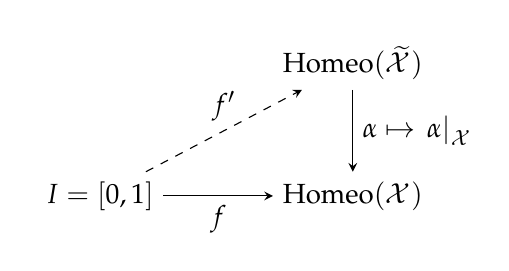
\begin{tikzpicture}
   \matrix (m) [matrix of math nodes,row sep=3em,column sep=4em,minimum width=2em] {
   	& \mathrm{Homeo}(\widetilde{\mathcal{X}}) \\
   	I = [0,1]  & \mathrm{Homeo}(\mathcal{X}) \\};
   \path[-stealth]
   (m-2-1.east|-m-2-2) edge node [below] {$f$}(m-2-2)
   (m-1-2) edge node [right] {$\al \mapsto \left.\a\right|_{\mathcal X}$} (m-2-2)
   (m-2-1)      edge [dashed]  node[above] {$f'$} (m-1-2);
   \end{tikzpicture}
   \hspace{\fill}
   \newline
   where $\mathrm{Homeo}$ means the group of homeomorphisms with {\it compact-open} topology (See \cite{spanier:at}). Above diagram has the following noncommutative generalization   
  \newline
  \hspace*{\fill}
  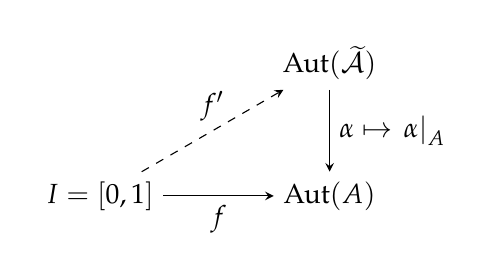
\begin{tikzpicture}
  \matrix (m) [matrix of math nodes,row sep=3em,column sep=4em,minimum width=2em] {
  	& \Aut(\widetilde{\A}) \\
  	I = [0,1]  & \Aut(A) \\};
  \path[-stealth]
  (m-2-1.east|-m-2-2) edge node [below] {$f$}(m-2-2)
  (m-1-2) edge node [right] {$\al \mapsto \left.\a\right|_{A}$} (m-2-2)
  (m-2-1)      edge [dashed]  node[above] {$f'$} (m-1-2);
  \end{tikzpicture}
  \hspace{\fill}
  \newline
   In the above diagram we require that $\al|_A \in \mathrm{Aut}\left(A\right)$ for any $\al \in \mathrm{Aut}\left(\widetilde{A}\right)$. The diagram means that $f'(t)|_{A} = f(t)$ for any $t \in [0,1]$. Noncommutative generalization of a locally compact space is a $C^*$-algebra, so  the generalization of $\mathrm{Homeo}(\mathcal{X})$ is the group  $\mathrm{Aut}(A)$ of *-automorphisms carries (at least) two different topologies making it into a topological group \cite{thomsem:ho_type_uhf}. The most important is {\it the topology of pointwise norm-convergence} based on the open sets
   \begin{equation*}
   	\left\{\left.\alpha \in \mathrm{Aut}(A) \ \right| \ \|\alpha(a)-a\| < 1 \right\}, \ a \in A.
   \end{equation*}
   \paragraph*{} The other topology is the {\it uniform norm-topology} based on the open sets
   \begin{equation}\label{aut_norm_eqn}
   	\left\{\alpha \in \mathrm{Aut}(A) \ \left| \ \sup_{a \neq 0}\ \|a\|^{-1} \|\alpha(a)-a\| < \varepsilon \right. \right\}, \ \varepsilon > 0
   \end{equation}
   which corresponds to following "norm"
   \begin{equation}\label{uniform_norm_topology_formula_eqn}
   	\|\alpha\|_{\text{Aut}} = \sup_{a \neq 0}\ \|a\|^{-1} \|\alpha(a)-a\| = \sup_{\|a\| =1}\  \|\alpha(a)-a\|.
   \end{equation}
   Above formula does not really means a norm because $\mathrm{Aut}\left(A\right)$ is not a vector space. Henceforth the uniform norm-topology will be considered only.

  \begin{definition}\label{upl_f_defn}
	Let $A \hookto \widetilde{A}$  be an inclusion of $C^*$-algebras. Let $f: [0,1] \to  \mathrm{Aut}\left({A}\right)$ be a continuous function such that $f\left( 0\right)= \Id_A$. If  there is a continuous map $\widetilde{f}: [0,1] \to  \mathrm{Aut}\left(\widetilde{A}\right)$ such that $\left.\widetilde{f}(t)\right|_A = f(t)$ for any $t \in \left[0,1\right]$ and $\widetilde{f}\left( 0\right)  = \Id_{\widetilde{A}}$ then we say that $\widetilde{f}$ is a $\pi$-\textit{lift} of $f$. If a lift $\widetilde{f}$ of $f$ is unique then  and map $\widetilde{f}: [0,1] \to  \mathrm{Aut}\left(\widetilde{A}\right)$ is said to be the \textit{unique $\pi$-lift} of $f$. If $\widetilde{f}$ is the unique $\pi$-lift of $f$ then we denote by 
	\be\label{upl_f_eqn}
	\lift_f \stackrel{\text{def}}{=}\widetilde{f}\left(1 \right).
	\ee
\end{definition}
 %  \begin{definition}\label{upl_defn}
%		Let $A \hookto \widetilde{A}$  be an inclusion of $C^*$-algebras.
%	We say that $\pi: A \hookto \widetilde{A}$   has the \textit{unique path lifting} if for any continuous $f: [0,1] \to  \mathrm{Aut}\left({A}\right)$ such that  $f\left( 0\right)= \Id_A$ there is the the unique $\pi$-lift of $f$. The property of unique path lifting will be denoted by $UPL$. The map $\widetilde{f}: [0,1] \to  \mathrm{Aut}\left(\widetilde{A}\right)$ is said to be the \textit{lift} of $f$. 
%\end{definition}
\begin{empt}\label{lift_group_empt}
	Let $\pi: A \hookto \widetilde{A}$  be an inclusion of $C^*$-algebras. Let both $f_1: [0,1] \to  \mathrm{Aut}\left({A}\right)$, $f_2: [0,1] \to  \mathrm{Aut}\left({A}\right)$ have unique $\pi$-lifts $\widetilde{f}_1$ and  $\widetilde{f}_2$ respectively. If $f_1* f_2: [0,1] \to  \mathrm{Aut}\left({A}\right)$, $\widetilde{f}_1* \widetilde{f}_2: [0,1] \to  \mathrm{Aut}\left(\widetilde{{A}}\right)$ are given by
\bean
\left( f_1* f_2\right) \left(t \right) =\left\{
\begin{array}{c l}
f_2\left( 2t\right)  &0 \le t \le \frac{1}{2}  \\
\\
f_1\left(2\left(t - \frac{1}{2} \right)  \right) f_2\left(1\right) & \frac{1}{2} < t \le 1
\end{array}\right.,\\
\left( \widetilde{f}_1* \widetilde{f}_2\right) \left(t \right) =\left\{
\begin{array}{c l}
	\widetilde{f}_2\left( 2t\right)  &0 \le t \le \frac{1}{2}  \\
	\\ \\
	\widetilde{f}_1\left(2\left(t - \frac{1}{2} \right)  \right) \widetilde{f}_2\left(1\right) & \frac{1}{2} < t \le 1
\end{array}\right.
\eean
then $\widetilde{f}_1* \widetilde{f}_2$ is the unique $\pi$-lift of $f_1*f_2$.
Hence one has $\lift_{f_1* f_2}= \lift_{f_1} \lift_{f_2}$.
It turns out that the set of elements $\lift_f$ is a subgroup of $\Aut\left(\widetilde{A}\right)$.
\end{empt}

\begin{defn}\label{lift_group_defn}
		Let $\pi: A \hookto \widetilde{A}$  be an inclusion of $C^*$-algebras then  the group of elements $\lift_f$ (cf. \ref{lift_group_empt}) is said to be the $\pi$-\textit{lift group}.
\end{defn}
\begin{lemma}\label{lift_commutes_lem}
		Let $A \hookto \widetilde{A}$  be an inclusion of $C^*$-algebras. Let $f: [0,1] \to  \mathrm{Aut}\left({A}\right)$ be a continuous function such that $f\left( 0\right)= \Id_A$ and $\widetilde{f}: [0,1] \to  \mathrm{Aut}\left(\widetilde{A}\right)$ is  the \textit{unique $\pi$-lift} of $f$. If $g \in G=\left\{\left. g \in \Aut\left(\widetilde{A} \right)~\right|~ ga = a;~~\forall a \in A\right\}$. Then one has $g\widetilde{f}\left( 1\right) = \widetilde{f}\left( 1\right)g$, i.e. $G$ commutes with the $\pi$-lift group.
\end{lemma}
\begin{proof}
If $\widetilde{f}': [0,1] \to  \mathrm{Aut}\left(\widetilde{A}\right)$ is given by $\widetilde{f}'(t)= g\widetilde{f}(t)g^{-1}$ then $\widetilde{f}'(t)|_A = \widetilde{f}(t)|_A$. From the Definition \ref{upl_f_defn} it turns out $\widetilde{f}'= \widetilde{f}$. It turns out $g\widetilde{f}(1)g^{-1}=\widetilde{f}'(1)=\widetilde{f}(1)$, i.e. one has $\widetilde{f}(1) = g\widetilde{f}(1)g^{-1}$ and, consequently  $\widetilde{f}(1)g = g\widetilde{f}(1)$.
\end{proof}
%\begin{empt}\label{loop_element_empt}
%Let	$\left(A, \widetilde{A}, G, \pi \right)$ be a noncommutaive finite-fold quasi-covering which  has the {unique path lifting}.
%For any $f: [0,1] \to  \mathrm{Aut}\left({A}\right)$ such that $f\left( 0\right)= f\left(1\right)= \Id_A$ and $\widetilde{f}: [0,1] \to  \mathrm{Aut}\left(\widetilde{A}\right)$ such that  that $\widetilde{f}(t)|_A = f(t)$ then $\al = \widetilde{f}\left( 0\right)$ is such that  $\al|_A = \Id_A$, i.e. $\al \in G$. %Moreover if $f': [0,1] \to  \mathrm{Aut}\left({A}\right)$, $f'': [0,1] \to  \mathrm{Aut}\left({A}\right)$ are such that 
%\end{empt}
%\begin{defn}\label{loop_element_defn}
%	Let us consider the situation \ref{loop_element_empt}.
%The element  $\al \in G$ given by \ref{loop_element_empt} is said to be a \textit{loop element}. We say that $\al$ \textit{corresponds} to $f$.
%Clearly a set $L$ of loop elements is a subgroup of $G$, which is said to be the \textit{loop subgroup}. 
%\end{defn}
%\begin{lem}\label{loop_normal_lem}
%	Let	$\left(A, \widetilde{A}, G, \pi \right)$ be a noncommutaive finite-fold quasi-covering which  has the {unique path lifting}. If  $f: [0,1] \to  \mathrm{Aut}\left({A}\right)$ such that $f\left( 0\right)= \Id_A$  and $\widetilde{f}: [0,1] \to  \mathrm{Aut}\left(\widetilde{A}\right)$ such that  that $\widetilde{f}(t)|_A = f(t)$ for any $t \in \left[0,1\right]$ and $\widetilde{f}\left( 0\right)  = \Id_{\widetilde{A}}$ then $g\widetilde{f}(t)g^{-1}= \widetilde{f}(t)$ for any $t \in  [0,1]$.
%\end{lem}
%\begin{proof}
%If $\widetilde{f}': [0,1] \to  \mathrm{Aut}\left(\widetilde{A}\right)$ is given by $\widetilde{f}'(t)= g\widetilde{f}(t)g^{-1}$ then $\widetilde{f}'(t)_A = \widetilde{f}(t)|_A$. From the Definition \ref{upl_defn} it turns out $\widetilde{f}'\cong \widetilde{f}$.
%\end{proof}
%\begin{cor}\label{loop_normal_cor}
%Let	$\left(A, \widetilde{A}, G, \pi \right)$ be a noncommutaive finite-fold quasi-covering which  has the {unique path lifting}. The loop subgroup $L \subset G$ is a normal subgroup of $G$.
%\end{cor}
%\begin{proof}
%Let $g \in G$ and $l \in L$ be any elements, and suppose that $l$ {corresponds} to $f: [0,1] \to  \mathrm{Aut}\left({A}\right)$. If $\widetilde{f}: [0,1] \to  \mathrm{Aut}\left(\widetilde{A}\right)$ is such that $\widetilde{f}(t)|_A = f(t)$ then $ g\widetilde{f}\left( t\right)g^{-1} = \widetilde{f}\left( t\right)$ for all $t \in \left[0,1 \right]$ in particular one has $ g\widetilde{f}\left( 1\right)g^{-1}=\widetilde{f}\left( 1\right)$, or equivalently $glg^{-1}= l$.
%\end{proof}

%\begin{remark}\label{lift_commute_g}
%From the Definition \ref{upl_defn} it turns out that path lift commutes with $G$ i.e. for any lift $\widetilde{f}: [0,1]\to \mathrm{Aut}\left(\widetilde{A}\right)$ and $g \in G$ the map $g\widetilde{f}: [0,1]\to \mathrm{Aut}\left(\widetilde{A}\right)$ is also a lift.
%\end{remark}
\begin{lemma}
		Let $\pi: A \hookto \widetilde{A}$  be an inclusion of $C^*$-algebras.
$f: [0,1] \to  \mathrm{Aut}\left({A}\right)$ be a continuous function such that $f\left( 0\right)= \Id_A$. If  there are two different $\pi$-lifts of $f$ then there is a nontrivial continuous  map: $\widetilde{f}:[0,1] \to  \mathrm{Aut}\left(\widetilde{A}\right)$ such that $\widetilde{f}|_A\left( t\right)  = \id_A$ for every $t \in \left[0,1\right]$.
\end{lemma}
\begin{proof}
	If $\widetilde{f}'$ and $\widetilde{f}''$ are different $\pi$-lifts of $f$ then the map $\widetilde{f}:[0,1] \to  \mathrm{Aut}\left(\widetilde{A}\right)$ given by $t \mapsto \widetilde{f}'\left( t\right)\left(  \widetilde{f}''\left( t\right) \right)^{-1}$ satisfies to conditions of this lemma.
\end{proof}
\begin{cor}\label{lift_unique_cor}
	Let $\pi: A \hookto \widetilde{A}$  be an inclusion of $C^*$-algebras, such that the group 
				\be\nonumber
	G = \left\{ \left.g \in \Aut\left(\widetilde{A} \right)~\right|~ ga = a;~~\forall a \in A\right\}
	\ee
	is finite,  and let   $f: [0,1] \to  \mathrm{Aut}\left({A}\right)$ be such that  $f\left( 0\right)= \Id_A$. If $\widetilde{f}$ is a $\pi$-lift of $f$ then   $\widetilde{f}$ is the unique $\pi$-lift of $f$.
\end{cor}
\begin{proof}
	If there are two different lifts of  $f$  then there is a nontrivial continuous  map: $\widetilde{f}:[0,1] \to  \mathrm{Aut}\left(\widetilde{A}\right)$ such that $\widetilde{f}|_A\left( t\right)  = \id_A$. For any $t \in [0,1]$ one has $\widetilde{f}\left(t \right) \in G$. Since $\widetilde{f}$ is not trivial, the group $G$ is not finite.
\end{proof}

%\begin{lemma}\label{w_path_lift_cor}
%	Let $\pi: A \hookto \widetilde{A}$  be an inclusion of $C^*$-algebras. Suppose $\widetilde{a} \in  \widetilde{A}$ is such that there  is a faithful representation $\rho: \widetilde{A} \to B\left(\H \right)$ such that $\rho\left( \widetilde{a}\right)  \in\rho\left(A \right)''$. If $f: [0,1] \to  \mathrm{Aut}\left({A}\right)$ such that  $f\left( 0\right)= \Id_A$ and both $\widetilde{f}_1, \widetilde{f}_2$ are $\pi$-lifts of $f$ are then $\widetilde{f}_1\left(t\right) \left(\widetilde{a}\right)=\widetilde{f}_2\left(t\right) \left(\widetilde{a}\right)$ for every $t \in [0,1]$. 
%\end{lemma}
%\begin{proof}
%	Since $A$ dense in $\rho\left(A \right)''$ the map $f$ can be uniquely extended up to a continuous map $f'': [0,1] \to  \mathrm{Aut}\left(\rho\left(A \right)''\right)$. From $\rho\left( \widetilde{a}\right)  \in\rho\left(A \right)''$ it turns out $\rho\left(\widetilde{f}_1\left(t\right) \widetilde{a}\right) = \rho\left(\widetilde{f}_2\left(t\right) \widetilde{a}\right)= f''\left( t\right) \left(\rho\left(\widetilde{a} \right) \right)$. Since $\rho$ is faithful one has $\widetilde{f}_1\left(t\right)\left(\widetilde{a}\right)=\widetilde{f}_2\left(t\right) \left(\widetilde{a}\right)$ for each $t \in [0,1]$.
%\end{proof}

%\begin{corollary}\label{borel_path_lift_cor}
%	Let $\pi: A \hookto \widetilde{A}$  be an inclusion of $C^*$-algebras. Suppose $\widetilde{a} \in  \widetilde{A}$ is such that there  is a normal $a \in A$ and Borel measured function $\phi$ such that  $\widetilde{a}= \phi\left( a\right)$. If $f: [0,1] \to  \mathrm{Aut}\left({A}\right)$ such that  $f\left( 0\right)= \Id_A$ and both $\widetilde{f}_1, \widetilde{f}_2$ are $\pi$-lifts of $f$ then $\widetilde{f}_1\left(t\right) \left(\widetilde{a}\right)=\widetilde{f}_2\left(t\right) \left(\widetilde{a}\right)$ for every $t \in [0,1]$.
%\end{corollary}

   \begin{thm}\label{comm_thm}
   	Let $p: \widetilde{\mathcal{X}} \to \mathcal{X}$ be a topological covering projection. Any path $\omega: I \to \mathrm{Homeo}(\mathcal{X})$ such that $\omega(0)=\mathrm{Id}_{\mathcal{X}}$ can be uniquely lifted to the path $\widetilde{\omega}: I \to \mathrm{Homeo}(\widetilde{\mathcal{X}})$ such that $\widetilde{\omega}(0)=\mathrm{Id}_{\widetilde{\mathcal{X}}}$ , i.e. $p(\widetilde{\omega}(t)(x)) = \omega(t)(p(x))$, $\forall t \in [0,1], \ \forall x \in \widetilde{\mathcal{X}}$. It means that the natural *-homomorphism $C_0\left({\mathcal{X}} \right) \hookto C_0\left( \widetilde{\mathcal{X}}\right) $ has the unique path lifting.
   \end{thm}
   \begin{proof}
   	Follows from theorem \ref{spanier_thm_un}.
   \end{proof}

   
   \section{Coverings of spectral triples}\label{triple_fin_cov}

  \paragraph*{}
 
 	Let  $\left( \A, \H, D\right)$ %, \left( \Ga, \right) J\right) $ 
 	be a spectral triple, and let $A$ is the $C^*$-norm completion of $\A$. Let $\left(A, \widetilde{A}, G \right)$ be an unital noncommutative finite-fold covering. Let $\rho: A \to B\left(\H \right)$ be a natural representation given by the spectral triple $\left( \A, \H, D\right)$, and let $\widetilde{\rho}: \widetilde{A} \to B\left( \widetilde{\H}\right)$ be a representation induced by the pair $\left( \rho,\left(A, \widetilde{A}, G \right) \right)$.  
 	The algebra $\widetilde{A}$ is a finitely generated projective $A$-module, it turns out following direct sum
 	$$
 	\widetilde{A} \bigoplus Q \cong A^n.
 	$$
 	of $A$-modules. So there is a projector $p \in \mathbb{M}_n\left(A \right)$ such that
 	$
 		\widetilde{A} \cong pA^n
 	$
 	as $A$-module.  $\A$ is dense in $A$ and $\A$ is closed with respect homomorphic calculus, it turns out that there is a projector $\widetilde{p} \in \mathbb{M}_n\left(\A \right)$ such that $\left\| \widetilde{p} - p\right\|  < 1$, so one has
 	$$
 		\widetilde{A} \cong	\widetilde{p}A^n.
 	$$
 	From $	\widetilde{A} \subset \End_A\left(	\widetilde{A} \right)$ and  $\End_A\left(	\widetilde{A} \right) = \widetilde{p}~\mathbb{M}_n\left(A \right)\widetilde{p} \subset \mathbb{M}_n\left(A \right)$ it follows that there is the following inclusion of $C^*$-algebras
 	$
 	\widetilde{A} \subset \mathbb{M}_n\left(A \right)
 	$. Both $\widetilde{A}$ and $\mathbb{M}_n\left(A \right)$ are finitely generated projective $A$ modules, it turns out that there is an $A$-module $P$ such that
 	$$
 	\widetilde{A} \bigoplus P \cong	\mathbb{M}_n\left(A \right) .
 	$$
 	Taking into account inclusions  $\widetilde{A} \subset \mathbb{M}_n\left(A \right)$ and $\mathbb{M}_n\left(\A \right) \subset \mathbb{M}_n\left(A \right)$ one can define the intersection of algebras
 \begin{equation}\label{a_smooth_eqn}
 	\widetilde{\A}= \widetilde{A} \bigcap \mathbb{M}_n\left(\A \right).
 \end{equation}
 From \cite{varilly_bondia} it turns out that $\mathbb{M}_n\left(\A \right)$ is closed with respect to holomorphic functional calculus.
 	Both $\mathbb{M}_n\left(\A \right)$ and $\widetilde{A}$ are closed with respect to holomorphic functional calculus, so $\widetilde{\A}$ is closed with respect to holomorphic functional calculus, i.e. $\widetilde{\A}$ is a pre-$C^*$-algebra. From 
 	$$
 	\mathbb{M}_n\left(\A \right) \cong \widetilde{\A} \bigoplus \left(P \bigcap 	\mathbb{M}_n\left(\A \right)\right) 
 	$$
 	it turns out that $\widetilde{\A}$ is a finitely generated projective $\A$ module.
 	
 	
  \begin{lemma}\label{dense_lem}
  	The algebra $\widetilde{\A}$ is a dense subalgebra of $\widetilde{A}$ with respect to the $C^*$-norm topology.
  \end{lemma}
\begin{proof}
	There is the isomorphism $A^{n^2}\approx \mathbb{M}_n\left(A \right)$ of right $A$-modules. Since $\widetilde{A}$ is a projective right $A$-module, there is a projector $p_M\in \mathbb{M}_{n^2}\left(A \right)$  it follows that 
	$$
\widetilde{A} \cong p_M A^{n^2}	
	$$
	The algebra $\mathbb{M}_{n^2}\left(\A \right)$ is dense in $\mathbb{M}_{n^2}\left(A \right)$, so there is a projector $\widetilde{p}_M\in \mathbb{M}_{n^2}\left(\A \right)$ such that such that $\left\| \widetilde{p}_M - p_M\right\|  < 1$, it turns out
\be\label{pm_eqn}
	\widetilde{\A} \cong \widetilde{p}_M \A^{n^2}
\ee
For any $\widetilde{a}\in \widetilde{A}$ there is a net $\left\{ \widetilde{a}_\a \in \mathbb{M}_{n}\left(\A \right)\right\}$ such that 
$$
\lim \widetilde{a}_\a = \widetilde{a}
$$
in sense of $C^*$-norm topology. The sequence can be regarded as a sequence $\left\{ \widetilde{a}_\a \in \A^{n^2}\right\}_{n \in \N}$. From \eqref{pm_eqn} it turns out that if $\widetilde{b}_\a=\widetilde{p}_M \widetilde{a}_\a \in \widetilde{A}$ then
$$
\lim \widetilde{b}_\a = \lim \widetilde{p}_M\widetilde{a}_\a = \widetilde{p}_M\lim \widetilde{a}_\a =  \widetilde{p}_M\widetilde{a}=\widetilde{a}.
$$
Otherwise from $\widetilde{a}_\a  \in \A^{n^2}$ and $\widetilde{p}_M\in \mathbb{M}_{n^2}\left(\A \right)$ it turns out that  $\widetilde{b}_\a =\widetilde{p}_M\widetilde{a}_\a  \in \A^{n^2}\cong \mathbb{M}_\a\left(\A \right)$, so one has  $\widetilde{b}_\a  \in \widetilde{A} \bigcap \mathbb{M}_\a\left(\A \right)\cong \widetilde{\A}$. Hence for any $\widetilde{a}\in \widetilde{A}$ there is a sequence $\left\{ \widetilde{b}_\a \in \widetilde{\A}\right\}_{n \in \N}$ such that
$$
\lim \widetilde{b}_\a = \widetilde{a}.
$$
\end{proof}

 \begin{definition}\label{smooth_defn}
 In the above situation we say that the unital noncommutative finite-fold covering $\left(A, \widetilde{A}, G \right)$ is \textit{smoothly invariant} if $G\widetilde{\A} = \widetilde{\A}$.
 \end{definition}
\begin{lem}\label{smooth_matr_lem}
	Let us use the above notation. Suppose that the right $A$-module $\widetilde{A}_A$ is generated by a finite set $\left\{\widetilde{a}_1, \dots, \widetilde{a}_n \right\}$, i.e. 
	$$
	\widetilde{A}_A = \sum_{j =1}^{n} \widetilde{a}_jA,
	$$
	such that following conditions hold:
	\begin{enumerate}
		\item[(a)] $\left\langle \widetilde{a}_j, \widetilde{a}_k\right\rangle_{\widetilde{A}} \in \A$ for any $j,k=1, \dots, n$,
		\item[(b)] The set $\left\{\widetilde{a}_1, \dots, \widetilde{a}_n \right\}$ is $G$-invariant, i.e. $g \widetilde{a}_j \in \left\{\widetilde{a}_1, \dots, \widetilde{a}_n \right\}$ for any $j = 1,\dots,n$ and $g \in G$.
	\end{enumerate}
Then following conditions hold:
\begin{enumerate}
	\item[(i)] 
	\be\label{smooth_cond_eqn}
	\widetilde{A} \bigcap \mathbb{M_n\left(\A \right) }= \left\{ 	\widetilde{a}\in 	\widetilde{A}~|~  \left\langle \widetilde{a}_j, \widetilde{a}\widetilde{a}_k\right\rangle_{\widetilde{A}} \in \A; ~\forall j,k =1, \dots, n\right\} 
	\ee
	\item[(ii)] The unital noncommutative finite-fold covering $\left(A, \widetilde{A}, G \right)$ is smoothly invariant.
\end{enumerate}
\end{lem}
\begin{proof}(i)
	If $S \in \End\left( \widetilde{A}\right)_A$ is given by  
\be\label{s_matr}
	S = \sum_{j=1}^{n}\widetilde{a}_j\left\rangle \right\langle\widetilde{a}_j
\ee
	then $S$ is self-adjoint. Moreover $S$ is represented by a matrix $\left\{S_{jk}=\left\langle \widetilde{a}_j, \widetilde{a}_k\right\rangle_{\widetilde{A}} \right\}_{j,k=1,\dots,n} \in \mathbb{M}_n\left( \A\right)$. From the Corollary 1.1.25  of \cite{jensen_thomsen:kk} it turns out that $S$ is strictly positive. Otherwise $\widetilde{A}_A$ is a finitely generated right $A$-module, so from the Exercise  15.O of \cite{wegge_olsen} it follows that $S$ is invertible, i.e. there is $T \in \End\left( \widetilde{A}\right)_A $ such that
	$$
	ST = TS = 1_{\End\left( \widetilde{A}\right)_A}.
	$$
	If we consider $S$ as element of $\mathbb{M}_m\left( \A\right)$ then the spectrum of $S$ is a subset of $\mathcal{U}_0 \bigcup \mathcal{U}_1 \subset \C$ such that
	\begin{itemize}
		\item Both $\mathcal{U}_0$ and $\mathcal{U}_1$ are open sets.
		\item $\mathcal{U}_0 \bigcap \mathcal{U}_1 = \emptyset$,
		\item $0 \in \mathcal{U}_0$ and $0$ is the unique point of the spectrum of $S$ which lies in $\mathcal{U}_0$.
	\end{itemize}
If $\pi, \psi$ are homomorphic functions on $\mathcal{U}_0 \bigcup \mathcal{U}_1$ given by 
\bean\nonumber
\phi|_{\mathcal{U}_0}= \psi|_{\mathcal{U}_0} \equiv 0,\\
\phi|_{\mathcal{U}_1}= 1,\\
\psi|_{\mathcal{U}_1}= z \mapsto \frac{1}{z}~.
\eean
Then following conditions hold:
\begin{itemize}
	\item $p = \phi\left( S\right)$ is a projector, such that $ \widetilde{A}_A \approx p A^n$ as a right $A$-module,
	\item $p \in \mathbb{M}_n\left(\A \right)$,
	\item $\psi\left( S\right) =T\in \mathbb{M}_n\left(\A \right)$ and $TS = ST = 1_{\End\left( \widetilde{A}\right)_A}$. 
\end{itemize}
If $\widetilde{a} \in A$ then from $TS = ST = 1_{\End\left( \widetilde{A}\right)_A}$ it turns out
$$
\widetilde{a} = TS\widetilde{a}ST = T\left( \sum_{j = 1}^n \widetilde{a}_j\left\rangle \right\langle\widetilde{a}_j\right)\widetilde{a}\left( \sum_{k = 1}^n \widetilde{a}_k\left\rangle \right\langle\widetilde{a}_k\right) T= TM^{\widetilde{a}}T
$$
where $M^{\widetilde{a}}\in  \mathbb{M}_n\left(A \right) $ is a matrix given by
$$
M^{\widetilde{a}}=\left\{M^{\widetilde{a}}_{jk}=\left\langle \widetilde{a}_j, \widetilde{a}\widetilde{a}_k\right\rangle_{\widetilde{A}} \right\}_{j,k=1,\dots,n}~.
$$
From $T \in \mathbb{M}_n\left(\A \right)$ it turns out that 
$$
M^{\widetilde{a}} \in \mathbb{M}_n\left(\A \right) \Rightarrow TM^{\widetilde{a}}T\in \mathbb{M}_n\left(\A \right). 
$$
Conversely from $S \in \mathbb{M}_n\left(\A \right)$ it follows that
$$
TM^{\widetilde{a}}T \in \mathbb{M}_n\left(\A \right)\Rightarrow STM^{\widetilde{a}}TS =M^{\widetilde{a}} \in \mathbb{M}_n\left(\A \right), 
$$
so one has
$$
M^{\widetilde{a}} \in \mathbb{M}_n\left(\A \right) \Leftrightarrow TM^{\widetilde{a}}T\in \mathbb{M}_n\left(\A \right). 
$$
Hence
$\widetilde{a} \in \mathbb{M}_n\left(\A \right)$ if and only if $\left\langle\widetilde{a}_j, \widetilde{a}\widetilde{a}_k\right\rangle_{\widetilde{A}}\in \A$ for any $j,k = 1, \dots n$. %From  $TS = ST = 1_{\End\left( \widetilde{A}\right)_A}$ it turns out 
%\be\label{aj_in_sm_eqn}
%\widetilde{a}_j = TS \widetilde{a}_j = T\left( \sum_{k = 1}^n \widetilde{a}_k\left\rangle \right\langle\widetilde{a}_k\right) \widetilde{a}_j = TM^j
%\ee
%where $M^j = \left\{m^j_{kl}\right\}_{k,l=1,\dots,n} \in \mathbb{M}_n\left(\A \right)$ is such that
%$$
%m^j_{kl}=\delta_{kj} \left\langle \widetilde{a}_j, \widetilde{a}_l\right\rangle_{\widetilde{A}} \in \mathbb{M}_n\left(\A \right).
%$$
%From $T \in \mathbb{M}_n\left(\A \right)$ and \eqref{aj_in_sm_eqn} it turns out $\widetilde{a}_j \in \mathbb{M}_n\left(\A \right)$ for any $j =1,\dots n$.
\\
(ii) Note that given by \eqref{finite_hilb_mod_prod_eqn} product is $G$-invariant, i.e. $\left\langle \widetilde{a} , \widetilde{b}  \right\rangle_{\widetilde{A}}= \left\langle g\widetilde{a} , g\widetilde{b}  \right\rangle_{\widetilde{A}}$ for any $g \in G$, it follows that
$$
\left\langle \widetilde{a}_j , \left( g\widetilde{a}\right)  \widetilde{a}_k  \right\rangle_{\widetilde{A}}=\left\langle g^{-1}\widetilde{a}_j , \widetilde{a} \left( g^{-1}\widetilde{a}_k\right)   \right\rangle_{\widetilde{A}}.
$$
Otherwise from  (b) it follows that there are $j',k' \in \left\{1, \dots, n\right\}$ such that
$\widetilde{a}_{j'}=g^{-1}\widetilde{a}_j$ and $\widetilde{a}_{k'}=g^{-1}\widetilde{a}_k$, hence $\left\langle \widetilde{a}_j , \left( g\widetilde{a}\right)  \widetilde{a}_k  \right\rangle_{\widetilde{A}} = \left\langle \widetilde{a}_{j'} ,  \widetilde{a}  \widetilde{a}_{k'}  \right\rangle_{\widetilde{A}}~$. So for any $g \in G$ the condition 
$$
\left\langle \widetilde{a}_j , \left( g\widetilde{a}\right)  \widetilde{a}_k  \right\rangle_{\widetilde{A}}\in \A,~~ \forall j,k =1, \dots n
$$
is equivalent to
$$
\left\langle \widetilde{a}_{j'} , \widetilde{a} \widetilde{a}_{k'}  \right\rangle_{\widetilde{A}}\in \A,~~ \forall j',k' =1, \dots n.
$$
It turns out that $g\left(  \widetilde{A} \bigcap \mathbb{M}_n\left(\A \right)\right) =\widetilde{A} \bigcap \mathbb{M}_n\left(\A \right)
$, or equivalently  $$G\left(  \widetilde{A} \bigcap \mathbb{M}_n\left(\A \right)\right) =\widetilde{A} \bigcap \mathbb{M}_n\left(\A \right)
,$$
hence from \eqref{a_smooth_eqn} one has
$$G\widetilde{\A}  =\widetilde{\A} 
.$$


 


\end{proof}
In the following text we suppose that  the unital noncommutative finite-fold covering $\left(A, \widetilde{A}, G \right)$ is smoothly invariant.
 	 From the Proposition \ref{conn_prop}  it follows that there is a connection
 	$$
 	\nabla' : \widetilde{\A} \to \widetilde{\A} \otimes_{\A} \Om^1_D.
 	$$
 
Let us define a connection
 	\begin{equation}\label{equiv_eqn}
 	\begin{split}
 	\widetilde{\nabla}:\widetilde{\A} \to \widetilde{\A} \otimes_{\A} \Om^1_D,\\
 	\widetilde{\nabla}\left(\widetilde{a} \right) = \frac{1}{\left|G \right|} \sum_{g \in G} g^{-1}\left(\nabla'\left( g\widetilde{a}\right) . \right)
 	\end{split}
 	\end{equation}
 	The connection $\widetilde{\nabla}$ is $G$-\textit{equivariant}, i.e.
 \be\label{equiv_conn_eqn}
 	\widetilde{\nabla}\left(g\widetilde{a} \right)= g\left( \widetilde{\nabla}\left(\widetilde{a} \right)\right) ; \text{ for any } g \in G, ~\widetilde{a} \in \widetilde{\A}.
 \ee
 	Let  $\H^\infty= \bigcap_{n =1}^\infty \Dom D^n$, and let us define an operator $\widetilde{D} : \widetilde{\A} \otimes_{\A} \H^\infty \to \widetilde{\A} \otimes_{\A} \H^\infty$ such that if $\widetilde{a} \in \widetilde{\A}$ and
 	\begin{equation*}
 	\begin{split}
 	\nabla\left( 	\widetilde{a}\right) = \sum_{j = 1}^m\widetilde{a}_j \otimes \om_j 
 	\end{split}
 	\end{equation*}
 	then
 	\begin{equation}\label{d_defn_eqn}
 	\widetilde{D}\left(	\widetilde{a} \otimes \xi \right) = \sum_{j = 1}^m\widetilde{a}_j \otimes \om_j\left( \xi\right) + \widetilde{a} \otimes D\xi.% \Leftrightarrow \left[\widetilde{D}, \widetilde{a}\right] = \widetilde{\nabla}\left( \widetilde{a}\right).
 	\end{equation}
 %	If $\widetilde{a}, 	\widetilde{b} \in 	\widetilde{\A}$ and $\xi \in \H^\infty$ then  from \eqref{d_defn_eqn} it follows that
 %	\be
 %	\begin{split}
 %	\left[\widetilde{D}, \widetilde{a} \right]\left(\widetilde{b} \otimes \xi \right) = \widetilde{D} \left( \left( \widetilde{a} \widetilde{b}\right)\otimes  \xi\right) - a \left( \right) 
 %	\end{split}
% \ee
 	The space $\widetilde{\A} \otimes_{\A} \H^\infty$ is a dense subspace of the Hilbert space $\widetilde{\H} = \widetilde{A} \otimes_{A} \H$.
 	It turns out  $\widetilde{D}$ can be regarded as an unbounded operator on $\widetilde{\H}$. 
 \begin{lem}\label{conn_exist_lem} If the unital noncommutative finite-fold covering $\left(A, \widetilde{A}, G \right)$ is smoothly invariant then there is the unique $G$-equivariant connection $$\widetilde{\nabla}:\widetilde{\A} \to \widetilde{\A} \otimes_{\A} \Om^1_D.$$
\end{lem}
\begin{proof} From the equation \eqref{equiv_eqn} it follows that a $G$-equivariant connection exists. Let us prove the uniqueness of it. 
	It follows from the Proposition \ref{conn_prop} that the space of connections is an affine space over the vector space $\Hom_{\sA}\left(\widetilde{\A}, \widetilde{\A} \otimes_{\A} \Om^1_D \right)$.  The space of $G$-equivariant connections is an affine space over the vector space $\Hom^{G}_{\sA}\left(\widetilde{\A}, \widetilde{\A} \otimes_{\A} \Om^1_D \right)$ of $G$-equivariant morphisms, i.e. morphisms in the category $\mathscr{M}^G_{\widetilde{\A}}$ (cf. \ref{fin_gal_cov_sec}). However from  $\ref{fin_gal_cov_sec}$ it follows that the category  $\mathscr{M}^G_{\widetilde{\A}}$ is equivalent to the category $\mathscr{M}_{\A}$ of $\A$-modules. It turns out that there is a 1-1 correspondence between connections
	$$
	\nabla:	\A \to \A \otimes_{\A} \Om^1_D= \Om^1_D
	$$
	and $G$-equivariant connections
	$$
	\widetilde{\nabla}:	\widetilde{\A} \to \widetilde{\A} \otimes_{\A} \Om^1_D.
	$$
	It follows that thee is the unique $G$-equivariant $\widetilde{\nabla}$ connection which corresponds to 
	\begin{equation*}
	\begin{split}
	\nabla:	\A \to \A \otimes_{\A} \Om^1_D= \Om^1_D,\\
	a \mapsto\left[ D, a\right]. 
	\end{split}
	\end{equation*}
	
\end{proof}
%The given by \eqref{d_defn_eqn} operator $\widetilde{D}$ satisfies to conditions (b) and (c) of the Definition \ref{triple_pre_lift_defn}, so one has a following theorem.
%\begin{thm}\label{st_fin_thm}
%If the unital noncommutative finite-fold covering $\left(A, \widetilde{A}, G \right)$ is smoothly invariant, 
% $\widetilde{\A}$ is given by \eqref{a_smooth_eqn}, $\widetilde{\H} = \widetilde{A} \otimes_A \H$ and $\widetilde{D}$ is given by \eqref{d_defn_eqn}, then  above construction yields  the unique spectral triple $\left( \widetilde{\A}, \widetilde{\H}, \widetilde{D}\right)$ which is a  $\left(A, \widetilde{A}, G \right)$. 
%	\end{thm}
\begin{defn}\label{triple_conn_lift_defn}
	The operator $\widetilde{D}$ given by \eqref{d_defn_eqn} is said to be the $\left(A, \widetilde{A}, G \right)$-\textit{lift} of $D$. The spectral triple $\left( \widetilde{\A}, \widetilde{\H}, \widetilde{D}\right)$  is said to be the  $\left(A, \widetilde{A}, G \right)$-\textit{lift} of $\left( \A, \H, D \right)$.
\end{defn}
%\begin{rem}
%	From \eqref{equiv_conn_eqn} it follows that the operator $\widetilde{D}$ is equivariant, i.e.
%	\be\label{equiv_d_eqn}
%	\widetilde{D}\left( g \widetilde{\xi}\right) = g \left( \widetilde{D}\widetilde{\xi}\right);~ \forall \widetilde{\xi} \in \Dom \widetilde{G}, ~ \forall g \in G.
%	\ee
%	There are two equivalent ways of definition of operator $\widetilde{D}$ from the Theorem  \ref{st_fin_thm}:
%	\begin{enumerate}
%		\item [(a)] Looking for an operator $\widetilde{ D}$ which satisfies to the Definition \ref{triple_lift_defn},
%		\item[(b)] Application of the equation \eqref{d_defn_eqn}.
%	\end{enumerate}
%\end{rem}
 
 
 
 \section{Finite noncommutative coverings and flat connections}\label{flat_sec}
 \subsection{Basic construction}\label{nc_flat_sec}
 \paragraph*{}
 Let $\left( \A, \H, D\right)$ be a spectral triple, let  $\left( \widetilde{\A}, \widetilde{\H}, \widetilde{D}\right)$ is the $\left(A, \widetilde{A}, G \right)$-lift of $\left( \A, \H, D \right)$. Let $V = \C^n$ and with left action of $G$, i.e. there is a linear representation $\rho: G \to GL\left(\C,n\right)$. Let $\widetilde{\mathcal E} =  \A \otimes \C^{n} \approx \widetilde{\A}^n$ be a free module over $\widetilde{\A}$, so $\widetilde{\mathcal E}$ is a projective finitely generated $\A$-module (because $\widetilde{ \A}$ is a finitely generated projective $\A$-module). Let $\widetilde{\nabla} : \widetilde{\mathcal E} \to \widetilde{\mathcal E} \otimes_{\widetilde{\A}} \Om^1_{\widetilde{D}}$ be the trivial flat connection. In \ref{triple_fin_cov} it is proven that $\Om^1_{\widetilde{D}} = \widetilde{\A}\otimes_{\A}\Om^1_{D}$ it follows that the connection $\widetilde{\nabla} : \widetilde{\mathcal E} \to \widetilde{\mathcal E} \otimes_{\widetilde{\A}} \Om^1_{\widetilde{D}}$ can be regarded as a map $\nabla':\widetilde{\mathcal E} \to \widetilde{\mathcal E} \otimes_{\widetilde{\A}} \widetilde{\A} \otimes_{\A} \Om^1_{\widetilde{D}}= \widetilde{\mathcal E} \otimes_{\A}\Om^1_{{D}}$, i.e. one has a connection
 \be\nonumber
 \nabla':\widetilde{\mathcal E} \to  \widetilde{\mathcal E} \otimes_{\A}\Om^1_{{D}}.
 \ee
 From $\widetilde{\nabla} \circ \widetilde{\nabla} |_{\mathcal E}=0$ it turns out that  $\nabla' \circ \nabla' |_{\mathcal E}=0$, i.e. $\nabla'$ is flat. There is the action of $G$ on $\widetilde{\mathcal E}= \widetilde{\A} \otimes \C^n$ given by 
 \be
 g\left( \widetilde{a}\otimes  x\right)   = g \widetilde{a} \otimes g x; ~~ \forall g \in G,~ \widetilde{a} \in \widetilde{\A}, ~ x \in \C^n.
 \ee
 Denote by
 \be
 \mathcal E = \widetilde{\mathcal E}^G = \left\{\widetilde{\xi} \in  \widetilde{\mathcal E}~|~ G\widetilde{\xi} = \widetilde{\xi}\right\}
 \ee
 Clearly $\mathcal E$ is an $\A$-$\A$-bimodule. For any $\widetilde{\xi} \in \widetilde{\mathcal E}$ there is the unique decomposition
 \be
 \begin{split}
 	\widetilde{\xi} = \xi + \xi_\perp, \\
 	\xi = \frac{1}{\left|G\right|}\sum_{g \in G} g \widetilde{\xi},\\
 	\xi_\perp = \widetilde{\xi} - \xi. 
 \end{split}
 \ee
 From the above decomposition it turns out the direct sum $\widetilde{\mathcal E} = \widetilde{\mathcal E}^G \bigoplus {\mathcal E}_\perp$ of $\A$-modules. So  $\mathcal E = \widetilde{\mathcal E}^G$ is a projective finitely generated $\A$-module, it follows that there is an idempotent $e \in \End_{\A}{\widetilde{\mathcal E}}$ such that $\mathcal E = e \widetilde{\mathcal E}$. The Proposition \ref{conn_prop} gives the canonical connection 
 \be\label{nc_flat_conn}
 \nabla : \mathcal E \to \mathcal E \otimes_{\A} \Om^1_D
 \ee
 which is defined by the connection $\nabla':\widetilde{\mathcal E} \to  \widetilde{\mathcal E} \otimes_{\A}\Om^1_{{D}}$ and the idempotent $e$.
 
 	\begin{lemma}\label{flat_lem}
 	If $\nabla:  \mathcal E \to \mathcal E \otimes_{\A} \Om^1$ is a trivial connection and $e \in \End_{\A}\left( \E\right)$ is an idempotent then the given by \eqref{idem_conn}
 	$$
 	\xi \mapsto \left(e \otimes 1 \right) \nabla \xi	
 	$$
 	connection $\nabla_e: e\mathcal E \to e\mathcal E \otimes \Om^1$  on $e\mathcal E$ is flat.
 \end{lemma} 
 \begin{proof}
 	From
 	$$
 	\left(e \otimes 1 \right)\left(\Id_{\mathcal E} \otimes d \right) \circ \left(e \otimes 1 \right)\left(\Id_{\mathcal E} \otimes d \right) = e \otimes d^2 = 0	
 	$$
 	it turns out that $\nabla_e \circ \nabla_e = 0$, i.e. $\nabla_e$ is flat.
 \end{proof}
 \begin{remark}
 	The notion of the trivial connection is an algebraic version of geometrical canonical connection explained in the Section \ref{geom_flat_subsec}.
 \end{remark}
 
 
  From the Lemma \ref{flat_lem} it turns out that the given by \eqref{nc_flat_conn} connection $\nabla$ is flat.
 \begin{definition}
 	We say that  $\nabla$ is a \textit{flat connection induced by} noncommutative covering $\left(A, \widetilde{A}, G\right)$ and the	linear representation $\rho: G \to GL\left(\C,n\right)$, or we say the $\nabla$ \textit{comes from the representation} $\rho: G \to GL\left(\C,n\right)$.
 \end{definition}
 \break

 
 \subsection{Mapping between geometric and algebraic constructions}
 
 \paragraph{}
 The geometric (resp. algebraic) construction of flat connection is explained in the Section \ref{geom_flat_subsec} (resp. \ref{nc_flat_sec}). Following table gives a mapping between these constructions.
 \newline
 
 \begin{tabular}{|c|c|c|}
 	\hline
 	&Geometry & Agebra\\
 	\hline
 	&	&\\
 	1&Riemannian manifold $M$.  & Spectral triple $\left(\Coo\left(M \right), L^2\left(M, \sS \right), \slashed D   \right)$. \\ & & \\
 	2&Topological covering $\widetilde{M} \to M$. & Noncommutative covering, \\ & & $\left(C\left(M \right), C\left(\widetilde{M} \right), G\left( \left.\widetilde{M}~\right|M\right)   \right),$  \\
 	& & given by the Theorem \ref{pavlov_troisky_thm}. \\ & & \\
 	3&Natural structure of Reimannian  & Triple $\left(\Coo\left(\widetilde{M} \right), L^2\left(\widetilde{M}, \widetilde{\sS} \right), \widetilde{\slashed D}   \right)$ is the\\
 	& manifold on the covering space $\widetilde{M}$.&  $\left(C\left(M \right), C\left(\widetilde{M} \right), G\left( \left.\widetilde{M}~\right|M\right)   \right)$ -lift
 	\\
 	&  & of $\left(\Coo\left(M \right), L^2\left(M, \sS \right), \slashed D   \right)$.\\ & & \\
 	4&Group homomorphism   & Action $ G\left( \left.\widetilde{M}~\right|M\right) \times \C^n \to \C^n$\\
 	&$ G\left( \left.\widetilde{M}~\right|M\right) \to GL\left(n, C \right)$ & \\ & & \\
 	5&Trivial bundle $\widetilde{M}\times \C^n$. & Free module $\Coo\left(\widetilde{M} \right) \otimes \C^n$. \\ & & \\
 	6&Canonical flat connection on $\widetilde{M}\times \C^n$ & Trivial flat connection on $\Coo\left(\widetilde{M} \right) \otimes \C^n$\\ & & \\
 	7&Action of $G\left( \left.\widetilde{M}~\right|M\right)$ on $\widetilde{M}\times \C^n$  & Action of $G\left( \left.\widetilde{M}~\right|M\right)$ on  $\Coo\left(\widetilde{M} \right) \otimes \C^n$\\ & & \\
 	8&Quotient space  & Invariant module    \\
 	& $P = \left( \widetilde{M}\times \C^n\right)/G\left( \left.\widetilde{M}~\right|M\right).$& $\mathcal E =  \left( \Coo\left( \widetilde{M}\right) \otimes \C^n\right)^{G\left( \left.\widetilde{M}~\right|M\right)}$ \\ & & \\
 	9&Geometric flat connection on $P$ & Algebraic flat connection on $\mathcal E$.\\ & & \\
 	\hline
 \end{tabular}
 
 
 
 
 
 
 
 
 
 
 
 
 
 
 
 \section{Unoriented spectral triples}\label{unoti_defn_sec}
 \paragraph*{}
 Let $M$ be an unoriented  Riemannian manifold, and let $\widetilde{M} \to M$ be a two-fold covering by oriented  Riemannian manifold $\widetilde{M}$ with Spin-structure. There is an action of $\Z_2 \times \widetilde{M} \to \widetilde{M}$ such that $M \cong \widetilde{M}/ \Z_2$. Let $\widetilde{\SS}$ be a Spin-bundle and $\left(\Coo\left( \widetilde{M}\right) , L^2\left(\widetilde{M}, \widetilde{\SS}\right), \widetilde{\slashed D}  \right)$ the spectral triple. Suppose  $g\in \Z_2$ is the unique nontrivial element and there is an $\Z_2$-equivariant action $\Z_2 \times L^2\left(\widetilde{M}, \widetilde{\SS}\right)\to L^2\left(\widetilde{M}, \widetilde{\SS}\right)$, i.e.
 \be\nonumber
 \begin{split}
 	g \left( \widetilde{a}\widetilde{\xi}\right)= \left(g \widetilde{a}\right) \left(g \widetilde{\xi}\right); ~~ \forall \widetilde{a} \in C\left(\widetilde{M} \right), ~~ \forall \widetilde{\xi} \in L^2\left(\widetilde{M}, \widetilde{\SS}\right),\\
 	\left( g \widetilde{\xi}, g\widetilde{\eta}\right) = \left( \widetilde{\xi}, \widetilde{\eta}\right);~~\forall \widetilde{\xi}, \widetilde{\eta} \in L^2\left(\widetilde{M}, \widetilde{\SS}\right);\\ \text{ where } \left(\cdot, \cdot \right) \text{ is the scalar product on }L^2\left(\widetilde{M}, \widetilde{\SS}\right).
 \end{split}
 \ee
 Suppose that $\widetilde{\slashed D}$ is $\Z_2$-invariant, i.e.
 $$
 g \left(\widetilde{\slashed D}\widetilde{\xi} \right) = \widetilde{\slashed D}\left(g \widetilde{\xi} \right); ~~  \forall \widetilde{\xi} \in \Dom \widetilde{\slashed D}. 
 $$
 Denote by
 \be\nonumber
 \begin{split}
 	L^2\left(\widetilde{M}, \widetilde{\SS}\right)^{\Z_2}= \left\{\widetilde{\xi} \in L^2\left(\widetilde{M}, \widetilde{\SS}\right)~|~g\widetilde{\xi} = \widetilde{\xi}\right\},\\
 	\slashed D = \widetilde{\slashed D}|_{L^2\left(\widetilde{M}, \widetilde{\SS}\right)^{\Z_2}}.
 \end{split}
 \ee
 The  Riemannian manifold $M$ is unoriented , it is reasonable to say that $$\left(\Coo\left(M \right), L^2\left(\widetilde{M}, \widetilde{\SS}\right)^{\Z_2}, \slashed D  \right)$$ is an unoriented spectral triple.  Following definition is motivated by the above construction.
 \begin{definition}\label{unoriented_defn}
 	Denote by $g \in \Z_2$ the unique nontrivial element.
 	An {\it unoriented spectral triple} $(\A, \H, D)$ consists of:
 	\begin{enumerate}
 		\item
 		a pre-$C^*$-algebra $\A$ with an involution $a \mapsto a^*$, equipped
 		with a faithful representation on:
 		\item
 		a \emph{Hilbert space} $\H$; and also
 		\item
 		a \emph{selfadjoint operator} $D$ on $\mathcal{H}$, with dense domain
 		$\Dom D \subset \H$, such that $a(\Dom D) \subseteq \Dom D$ for all 
 		$a \in \mathcal{A}$.
 		\item An unital oriented spectral triple $\left(\widetilde{\A}, \widetilde{\H}, \widetilde{D} \right)$ which satisfies to described in \cite{hajac:toknotes,varilly:noncom} axioms, such that following conditions hold:
 		\begin{enumerate}
 			\item  There are  actions $\Z_2 \times \widetilde{\A} \to  \widetilde{\A} $,  $\Z_2 \times \widetilde{\H} \to  \widetilde{\H} $, such that
 			\be\label{main_def_1_eqn}
 			\begin{split}
 				g \left( \widetilde{a}\widetilde{\xi}\right)= \left(g \widetilde{a}\right) \left(g \widetilde{\xi}\right); ~~ \forall \widetilde{a} \in \widetilde{\A}, ~~ \forall \widetilde{\xi} \in\widetilde{\H},\\
 				\left( g \widetilde{\xi}, g\widetilde{\eta}\right) = \left( \widetilde{\xi}, \widetilde{\eta}\right);~~\forall \widetilde{\xi}, \widetilde{\eta} \in \widetilde{\H},,\\ \text{ where } \left(\cdot, \cdot \right) \text{ is the scalar product on }\widetilde{\H},
 			\end{split}
 			\ee
 			
 			\be\label{main_def_2_eqn}
 			\begin{split}
 				g \left(\widetilde{ D}\widetilde{\xi} \right) = \widetilde{ D}\left(g \widetilde{\xi} \right); ~~  \forall \widetilde{\xi} \in \Dom \widetilde{ D}. 
 			\end{split}
 			\ee
 			\item There are isomorphisms
 			\be\label{main_def_3_eqn}
 			\begin{split}
 				\A \cong \widetilde{\A}^{\Z_2} \stackrel{\text{def}}{=}\left\{\widetilde{a} \in \widetilde{\A}~|~ g\widetilde{a} = \widetilde{a} \right\},\\
 				\H \cong \widetilde{\H}^{\Z_2}\stackrel{\text{def}}{=} \left\{\widetilde{\xi} \in \widetilde{\H}~|~ g\widetilde{\xi} = \widetilde{\xi} \right\}.
 			\end{split}
 			\ee
 			\item If $A$ (resp. $\widetilde{A}$) is a $C^*$-norm completion of $\A$ (resp. $\widetilde{\A}$) then the triple $\left(A, \widetilde{A}, \Z_2 \right)$ is an unital noncommutative finite-fold  covering and a following condition holds
 			\be\label{main_def_4_eqn}
 			\begin{split}
 				\A= A\bigcap \widetilde{\A}.
 			\end{split}
 			\ee
 			\item 
 			\be\label{main_def_5_eqn}
 			\begin{split}
 				D = \widetilde{ D}|_{\H}=\widetilde{ D}|_{\widetilde{\H}^{\Z_2}}.
 			\end{split}
 			\ee
 		\end{enumerate}
 		
 		
 	\end{enumerate}
 \end{definition}
 
 
 

 \chapter{Noncommutative infinite coverings}\label{cov_inf_chap}
 \section{Basic definitions}\label{inf_bas_constr_sec}
 \paragraph*{}
 This section contains a noncommutative generalization of infinite coverings.
 \begin{definition}\label{compliant_covering_defn}
 	Let us consider the following diagram\\
 	\newline
 	\begin{tikzpicture}
 	\matrix (m) [matrix of math nodes,row sep=3em,column sep=4em,minimum width=2em]
 	{
 		\widetilde A_1  &  & \widetilde A_2\\
 		& A & \\};
 	\path[-stealth]
 	(m-1-1) edge[dashed] node [above] {$\pi^1_2$} (m-1-3)
 	(m-2-2) edge node [left]  {$\pi_1~~$} (m-1-1)
 	(m-2-2) edge node [right] {$~~\pi_2$} (m-1-3);
 	%\draw[dashed,->]   (m-1-1) -- (m-1-3);
 	\end{tikzpicture}
 	\\
 	where $A$, $\widetilde A_1$, $\widetilde A_2$ are $C^*$-algebras and $\pi_1$, $\pi_2$, are noncommutative finite-fold coverings. We say that the unordered pair $\left( \pi_1,\pi_2\right) $ is \textit{compliant} if  it satisfies to following conditions:
 	\begin{enumerate}
 		\item[(a)]
 		If there is a *-homomorphism $\pi^1_2: \widetilde A_1 \to \widetilde A_2$ such that $\pi_2 = \pi^1_2 \circ \pi_1$ then $\pi^1_2$ is  a noncommutative finite-fold  covering (cf. Definition \ref{fin_defn}).
 		\item[(b)] Following condition holds
 		\be\label{g_sur_eqn}
 		G\left(\left.\widetilde A_2~\right|A \right)\pi^1_2\left(\widetilde A_1\right)=  \pi^1_2\left(\widetilde A_1\right).
 		\ee 
 		\item[(c)] From \eqref{g_sur_eqn} it turns out that there is the homomorphism $h: G\left(\left.\widetilde A_2~\right|A \right)\to 	G\left(\left.\widetilde A_1~\right|A \right)$ such that 
 		\be\label{g_sur_pi_eqn}
 		\pi^1_2\left( h\left(g \right)a_1\right) = g \circ \pi^1_2\left(a_1 \right)
 		\ee 
 		for each $a_1 \in \widetilde A_1$.  
 		We claim that $h$ is surjective. 
 		\item[(d)] If  $\rho: \widetilde A_1 \to \widetilde A_2$ is any *-homomorphism  such that $\pi_2 = \rho \circ \pi_1$ then there is the unique $g \in 	G\left(\left.\widetilde A_1~\right|A \right)$ such that 
 		\be\label{compliant_covering_g_eqn}
 		\rho =  \pi^1_2 \circ g.
 		\ee
 	\end{enumerate}
 	
 \end{definition}
 \begin{definition}\label{compliant_comes_defn}
 	In the situation of the Definition \ref{compliant_covering_defn} we say that the homomorphism $h: G\left(\left.\widetilde A_2~\right|A \right)\to 	G\left(\left.\widetilde A_1~\right|A \right)$ which satisfies to \eqref{g_sur_pi_eqn} \textit{comes} from $\pi^1_2$.
 \end{definition}
 \begin{remark}
 	From the Definition \ref{compliant_covering_defn} it turns out that if $\rho': \widetilde A_1 \to \widetilde A_2$ and $\rho': \widetilde A_2 \to \widetilde A_1$ are *-homomorphisms such that $\pi_2 = \rho' \circ \pi_1$ and $\pi_1 = \rho'' \circ \pi_2$ then both $\rho'$ and $\rho''$ are *-isomorphisms.
 \end{remark}
 
 
 
 \begin{definition}\label{comp_defn}
 	Let $\La$ be a directed set (cf. Definition \ref{directed_set_defn}) such that there is the unique minimal element $\la_{\mathrm{min}} \in \La$.
 	Let $A$ be a $C^*$-algebra.  Let us consider a set noncommutative finite-fold coverings $\mathfrak{S}=\left\{ \pi_{\la}:A \hookto A_{\la}\right\}_{\la \in \La}$ indexed by  $\La$ such that $A_{\la_{\mathrm{min}}}= A$, and $\pi_{\la_{\mathrm{min}}}= \Id_A$. We do not claim that any noncommutative finite-fold covering $A \to \widetilde{A}$ belongs to $\mathfrak{S}$. Suppose that  following conditions hold:
 	\begin{enumerate}
 		\item[(a)] For any $\mu, \nu \in \La$ a pair $\left( \pi_\mu, \pi_\nu\right)$ is compliant (cf. Definition \ref{compliant_covering_defn}).
 		\item [(b)]
 		For  $\mu, \nu \in \La$ one has
 		\be\label{fg_ord_eqn}
 		\begin{split}
 			\mu \ge \nu  \text{ if and only if there is an *-homomorphism } \pi: A_\nu \hookto A_\mu; \\
 			\text{ such that } \pi_\mu = \pi \circ \pi_\nu.
 		\end{split}
 		\ee
 	\end{enumerate}
 	The set 
 	$\mathfrak{S}=\left\{ \pi_{\la}:A \hookto A_{\la}\right\}_{\la \in \La}$, or equivalently $$\mathfrak{S}=\left\{ \left( A , A_{\la}, G\left(\left.A_\la~\right|A \right) , \pi_{\la}\right) \right\}_{\la \in \La}$$
 	is said to be an \textit{algebraical  finite covering category}. 
 	We write $\mathfrak{S} \in \mathfrak{FinAlg}$.
 \end{definition}
% \begin{definition}\label{comp_defn}
% 	An algebraical finite precovering category said to be an \textit{algebraical  finite covering category} if all morphism of it are finite-fold coverings.   We write $\mathfrak{S} \in \mathfrak{FinAlg}$
% \end{definition}
 \begin{definition}\label{comp_pt_defn}
 	A subcategory $\mathfrak{S}^{\text{pt}}$  of an algebraical  finite covering category $\mathfrak{S}$  is said to be a \textit{pointed algebraical  finite covering category}  if it is equivalent to the pre-order category given by $\La$ (cf. Definition \ref{preordercat_defn} and Remark \ref{pre_order_rem}).  We write $\mathfrak{S}^{\text{pt}} \in \mathfrak{FinAlg}^{\text{pt}}$ We use following notation
 	\be\label{comp_pt_eqn}
 	\begin{split}
 	\mathfrak{S}^{\text{pt}} = \left(\left\{\pi_\la: A \hookto A_\la \right\}_{\la \in \La}, \left\{\pi^\mu_\nu: A_\mu \hookto A_\nu\right\}_{\substack{\mu, \nu \in \La\\ \nu > \mu}}\right),\\
 	\text{or simply} \quad \mathfrak{S}^{\text{pt}} = \left(\left\{\pi_\la: A \hookto A_\la \right\}, \left\{\pi^\mu_\nu\right\}\right).
 	\end{split}
 	\ee
 \end{definition}
 \begin{remark}\label{comp_pt_rem}
 	The Definition \ref{comp_pt_defn} means that for any $\mu \ge \nu$ the category $\mathfrak{S}^{\text{pt}}$ contains the unique *-homomorphism $\pi^\nu_{ \mu}: A_\nu \hookto A_\mu$. The family of $\left\{\pi^\nu_{ \mu}\right\}$ of *-homomorphisms  is said to be a \textit{base-point}.
 \end{remark}
 
 \begin{empt}\label{inv_g_lim_empt} Let us consider the situation of the Definition \ref{comp_pt_defn}.
 	If $\mu, \nu \in \La$ and $\mu > \nu$. Denote by   $h^\mu_\nu:  G\left(\left.A_\mu~\right|A \right) \to  G\left(\left.A_\nu~\right|A \right)$ the surjective homomorphism which comes from $\pi^\nu_\mu$ (cf. Definition \ref{compliant_comes_defn}).
 \end{empt}
 \begin{lemma}\label{inv_g_lim_lem}
 	Let us use notation of \ref{inv_g_lim_empt}. If $\mu,\la, \nu$ are such that $\mu > \la > \nu$ then $h^\mu_\nu = h^\mu_\la \circ h^\la_\nu$. 
 \end{lemma}
 \begin{proof}
 	From the  equation \eqref{g_sur_pi_eqn} it turns out that for all $a_\nu \in A_\nu$ and $g_\mu \in  G\left(\left.A_\mu~\right|A \right)$ one has
 	\bea\label{h_array_eqn}
 	\pi^\nu_\mu\left( h^\mu_\nu\left( g_\mu\right)  a_\nu\right)=g_\mu \circ \pi^\nu_\mu\left( a_\nu\right),\\
 	\label{h_array1_eqn}
 	\pi^\nu_\la\left( h^\la_\nu\left(h^\mu_\la\left(  g_\mu\right) \right)  a_\nu\right)=h^\mu_\la\left(  g_\mu\right) \circ \pi^\nu_\la\left( a_\nu\right),\\
 	\label{h_array2_eqn}
 	\pi^\la_\mu\left(h^\mu_\la\left( g_\mu\right)\pi^\nu_\la \left(  a_\nu\right) \right)=  g_\mu \circ \pi^\la_\mu\left( \pi^\nu_\la \left(  a_\nu\right)\right)= g_\mu \circ \pi^\nu_\mu \left(  a_\nu\right).
 	\eea
 	If we substitute $h^\mu_\la\left( g_\mu\right)\pi^\nu_\la \left(  a_\nu\right)$ in the left part of \eqref{h_array2_eqn} by the left part of \eqref{h_array1_eqn} and taking into account $\pi^\la_\mu\circ\pi^\nu_\la=\pi^\nu_\mu$ one has
 	\be\label{h_array3_eqn}
 	\pi^\la_\mu\left(\pi^\nu_\la\left( h^\la_\nu\left(h^\mu_\la\left(  g_\mu\right) \right)  a_\nu\right) \right)= \pi^\nu_\mu\left( h^\la_\nu\circ h^\mu_\la\left(  g_\mu\right)   a_\nu\right) = g_\mu \circ \pi^\nu_\mu \left(  a_\nu\right).\\
 	\ee
 	Comparison of \eqref{h_array_eqn} and \eqref{h_array3_eqn} yields $h^\mu_\nu = h^\mu_\la \circ h^\la_\nu$.
 \end{proof}
 
 
 \begin{defn}\label{inv_g_lim_rem}
 	From the Lemma \ref{inv_g_lim_lem} it turns out that one can define surjecive homomorphisms  $h^\mu_\nu:  G\left(\left.A_\mu~\right|A \right) \to  G\left(\left.A_\nu~\right|A \right)$ the surjective homomorphism which come from $\pi^\nu_\mu$, hence there is the inverse limit 
 	$$
 	\widehat{G}=	\varprojlim_{\la \in \La} G\left(\left.A_\la~\right|~A\right)
 	$$
 	of groups. For any $\la \in \La$ there is the surjecive homomorphism 
 	\be\label{h_la_eqn}
 	h_\la:\widehat{G}\to G\left(\left.A_\la~\right|~A\right)
 	\ee
 	Wa say that the  inverse limit \textit{comes} from the base point $\left\{\pi^\nu_\mu\right\}$ (cf Remark \ref{comp_pt_rem}).
 \end{defn}
 
 \begin{lemma}\label{base_point_change_lem}
 	Let 
 	$\mathfrak{S}=\left\{ \left( A , A_{\la},  G\left(\left.A_\la~\right|A \right), \pi_{\la}\right) \right\}_{\la \in \La}\in \mathfrak{FinAlg}$.
 	be an {algebraical  finite covering category}.	Consider two pointed subcategories $\mathfrak{S}^{\text{pt}}_\pi$, $\mathfrak{S}^{\text{pt}}_\rho$ having morphisms $\left\{\pi^\nu_\mu: A_{\nu}\hookto A_{
 		\mu}\right\}$ and $\left\{\rho^\nu_\mu: A_{\nu}\hookto A_{
 		\mu}\right\}$.
 	Suppose that both $$\left\{ d^\mu_{\nu} : G\left(\left.A_\mu~\right|A\right) \to G\left(\left.A_\nu~\right|A\right)\right\}  \text{ and }\left\{ e^\mu_{\nu} : G\left(\left.A_\mu~\right|A\right) \to G\left(\left.A_\nu~\right|A\right)\right\} $$ are surjecive homomorphisms which come from $\left\{\pi^\nu_\mu\right\}$ and $\left\{\rho^\nu_\mu\right\}$ respectively. 	Suppose that both $\widehat{G} = \varprojlim_{\la \in \La} G\left(\left.A_\la~\right|A\right)$ and $\widehat{H} = \varprojlim_{\la \in \La} G\left(\left.A_\la~\right|A\right)$ are inverse limits which come from $\left\{ d^\mu_{\nu} \right\} $ and $\left\{ e^\mu_{\nu} \right\} $ respectively. If 
 	$d_\la :\widehat{G}\to G\left(\left.A_\nu~\right|A\right)$ and $e_\la :\widehat{H}\to G\left(\left.A_\nu~\right|A\right)$ are natural surjective homomorphisms then there is the bijective map $\phi: \widehat{G} \xrightarrow{\approx} \widehat{H}$ and $\widehat{g}\in \widehat{G}$ such that
 	\bea\label{base_point_change_lem_eqn}
 	e_\la\circ \phi = d_\la \circ \widehat{g},\\
 	\label{base_point_change_p_lem_eqn}
 	\rho^\nu_\mu = 	\pi^\nu_\mu \circ d_\nu\left(\widehat{g} \right) \quad \forall \mu > \nu 
 	\eea
 \end{lemma}
 \begin{proof}
 	If $\mu \ge \nu$ then there is $g_\nu \in G\left(\left.A_\nu~\right|A\right)$ such that
 	\be\label{base_point_change_p_eqn}
 	\rho^\nu_\mu =   \pi^\nu_\mu \circ g_\nu.
 	\ee From $\pi^\nu_\mu = \pi^\la_\mu \circ \pi^\nu_\la$ and $\rho^\nu_\mu = \rho^\la_\mu \circ \rho^\nu_\la$ one has $d^\mu_\nu\left(g_\mu\right)= g_\nu$. The family $\left\{g_\la\right\}$ gives an element $\widehat{g}\in \widehat{G}$. Any $\widehat{g}' \in \widehat{G}$ corresponds to a family $\left\{g'_\la\right\}_{\la \in \La}$ such that $d^\mu_\nu\left(g'_\mu \right) = g'_\nu$. Otherwise there is the family $\left\{g''_\la\right\}_{\la \in \La}$ such that $g''_\la = g'_\la \circ d_\la \left(  \widehat{g}\right)$ and $e^\mu_\nu\left(g''_\mu \right) = g''_\nu$. The family $\left\{g''_\la\right\}$ uniquely defines the element $\widehat{g}'' \in \widehat{H}$. In result one has the  bijective map
 	\bean
 	\phi: \widehat{G} \xrightarrow{\approx} \widehat{H},\\
 	\widehat{g}' \mapsto \widehat{g}''
 	\eean 
 	which satisfies to the equation \eqref{base_point_change_lem_eqn}. The equation \eqref{base_point_change_p_lem_eqn} follows from \eqref{base_point_change_p_eqn}.
 \end{proof}
 \begin{rem}\label{base_point_change_gr_rem}
 	The map $\phi$ induces the isomorphism of groups
 	\be\label{base_point_change_rem_eqn}
 	\begin{split}
 		\varphi: \widehat{G} \xrightarrow{\approx} \widehat{H},\\
 		\widehat{g}^{~-1}	\widehat{g}'\widehat{g} \mapsto \phi\left( 	\widehat{g}'\right) 
 	\end{split}
 	\ee
 \end{rem}
 
 \begin{rem}\label{base_point_change_rem}
 	Let 
 	$\mathfrak{S}=\left\{ \left( A , A_{\la},  G\left(\left.A_\la~\right|A\right), \pi_{\la}\right) \right\}_{\la \in \La}\in \mathfrak{FinAlg}$.
 	be an {algebraical  finite covering category}. If both 
 	$\left\{\pi^\nu_\mu\right\}$ and $ \left\{\rho^\nu_\mu\right\}$ are base-points of $\mathfrak{S}$ then from the Lemma \ref{base_point_change_lem} it turns out the category $\left( \mathfrak{S}, \left\{\pi^\nu_\mu\right\}\right)$ is equivalent to $\left( \mathfrak{S}, \left\{\rho^\nu_\mu\right\}\right)$.
 \end{rem}
 %\begin{defn}\label{base_point_change_defn}
 %	Let $\left(\mathfrak{S}, \left\{\pi^\nu_\mu\right\} \right)\in P$-$\mathfrak{FinAlg}$ to be a  {pointed algebraical  finite covering category}. For any $\widehat{g}\in 	\varprojlim_{\la \in \La} G\left(\left.A_\la~\right|~A\right)$ there is the base point $\left\{\rho^\nu_\mu\right\}$ given by
 %	\be\label{base_point_change_eqn}
 %	\rho^\nu_\mu = \pi^\nu_\mu\circ h_\nu \left( \widehat{g}\right) 
 %	\ee
 %	The given by \eqref{base_point_change_defn} replacement of base point  is said to be a \textit{change of base point} (\textit{associated with} $\widehat{g}$).
 %\end{defn}
 %\begin{remark}
 %Any $\widehat{g}\in \widehat{G}$ yields a {change of base point}
 %\end{remark}
 
 \begin{remark}
 	There is a  functor from $ \mathfrak{S}^{\text{pt}} = \left\{\left\{\pi_\la: A \hookto A_\la \right\}, \left\{\pi^\mu_\nu\right\}\right\}$  to the category of finite groups and epimorphisms. The functor is given by
 	\bean
 	\left(A \hookto A_\la \right) \mapsto G\left(\left.A_\la~\right|A \right);\\
 	\left( \pi^\mu_\nu: A_\nu \hookto A_\mu\right)  \mapsto \left(h^\mu_\nu : G\left(\left.A_\mu~\right|~A\right)\to G\left(\left.A_\nu~\right|~A\right) \right). 
 	\eean
 \end{remark}
 
 
 
 
 
% \begin{remark}\label{cofinal_rem}
% 	If $\La' \subset \La$ is a {cofinal} subset then $\widehat{A} = C^*\text{-}\varinjlim A_{\la}$  be the $C^*$-inductive limit (cf. Definition \ref{inductive_lim_defn}), and suppose that $\widehat{G}= \varprojlim G\left(\left.A_{\la}\right|A \right) $
% 	\be\label{cofinal_eqn}
% 	\begin{split}
% 		C^*\text{-}\varinjlim_{\La} A_{\la} = 	C^*\text{-}\varinjlim_{\La'} A_{\la'},\\
% 		\varprojlim_{\la \in \La}  G\left(\left.A_{\la}\right|A \right)= \varprojlim_{ \La'}  %G\left(\left.A_{\la}\right|A \right).
% 	\end{split}
 %	\ee
 %	(cf. Proposition \ref{inductive_lim_prop}).
% \end{remark}
 \begin{remark}\label{coherent_rem}
 	If $\nu \ge \mu$ then since $\mathfrak{S}^{\text{pt}}$ contains the unique injective *-homomorphism $\pi^\mu_{ \nu}: 	A_\mu \hookto A_\nu$, we substitute following equations
 	\be\label{coherent_replace_s_eqn}
 	\begin{split}
 		\pi^\mu_{ \nu}: 	A_\mu \hookto A_\nu,\\
 		\pi^\mu_{ \nu}\left( 	a_\mu\right)  = \sum_{g\in G\left(\left.A_\mu~\right|~A_\nu \right)}ga_\nu
 	\end{split}
 	\ee
 	by
 	\be\label{coherent_replace_eqn}
 	\begin{split}
 		A_\mu \subset A_\nu,\\
 		a_\mu = \sum_{g\in G\left(\left.A_\mu~\right|~A_\nu \right)}ga_\nu
 	\end{split}
 	\ee	
 \end{remark}
 
 
 
% For any inclusion $A \hookto A'$ of $C^*$-algebras one has the natural inclusion of $C^*$-Hilbert modules
% \be\label{hilb_inc_eqn}
 %\ell^2\left(A \right) \hookto \ell^2\left(A'\right).
% \ee
% From $AM\left(A \right)  = A$ it turns out that
% \be\label{a_ell_eqn}
% A \ell^2\left(M\left(A \right)\right) \subset \ell^2\left( A\right)
% \ee
 
 \begin{definition}\label{special_set_defn}
 	Let $\mathfrak{S}^{\mathrm{pt}}=\left(\left\{\pi_\la: A \hookto A_\la \right\}, \left\{\pi^\mu_\nu\right\}\right)\in \mathfrak{FinAlg}^{\mathrm{pt}}$  be a  {pointed algebraical  finite covering category}. Let $A^+_{\la}$ be the minimal unitization of $A_\la$ (cf. Definition \ref{multiplier_min_defn}). 
 	A  family $\left\{a_\la \in A_{\la+}\right\}_{\la \in \La}$ of positive elements is \textit{special}  if following conditions hold:
 	\begin{enumerate}
 		\item[(a)]
 		\be\label{spec_a_eqn}
\forall \mu, \nu \in \La \quad \mu < \nu \quad  \Rightarrow	\quad 	a_\mu = \sum_{g\in G\left(\left.A_\mu~\right|~A_\nu \right)}ga_\nu
 		\ee
 		\item[(b)] 		If $f_\eps: \R \to \R$ is a continuous function given by 
 		\begin{equation}\label{f_eps_eqn}
 			f_\eps\left( x\right)  =\left\{
 			\begin{array}{c l}
 				0 &x \le \eps \\
 				x - \eps & x > \eps
 			\end{array}\right.
 		\end{equation}\label{spec_el_eqn}
 		then for any $\la, \mu \in \La$ such that $\mu \ge  \la$ and for all $z \in A_\la^+$  the following net
 		\begin{equation*}
 			\left\{\sum_{g\in G\left(\left.A_\nu~\right|~A_\mu \right)} gf_\eps\left( z^* a_\nu z\right)   \right\}_{\nu\ge \mu} \subset A_\mu,\\
 		\end{equation*}
 		is $C^*$-norm convergent, i.e. there is the following $C^*$-norm limit
 		\be\label{spec_el_lim_eqn}
 		\begin{split}
 			\lim_{\nu > \mu}~\sum_{g\in G\left(\left.A_\nu~\right|~A_\mu \right)} gf_\eps\left( z^* a_\nu z\right) \in A_\mu.
 		\end{split}
 		\ee
 		\item[(c)] For all $\eps > 0$, $\la_0 \in \La$ and
 		for every $z \in A_{\la_0}^+$ there is $\la \in \La$ such that $\la \ge \la_0$ and the following condition holds
 		\be\label{special_set_eqn}
\forall \mu, \nu \in \La \quad	\nu \ge \mu \ge \la  \Rightarrow  \left\|\left(z^* a_\mu z\right)^2  - \sum_{g \in G\left(\left.A_\nu\right|A_\mu\right)} g\left( z^* a_\nu z\right)^2\right\| < \eps.
 		\ee
 %		\item[(d)] If $\eps > 0$ and $a^\eps_\la = 	\lim_{\mu > \la}~\sum_{g\in G\left(\left.A_\mu~\right|~A_\la \right)} gf_\eps\left( a_\mu  \right)   \in A_\la$ then the family $\left\{a^\eps_\la\right\}$ satisfies to the conditions (a)-(c) of this definition. CONTRADICTS WITH a) !!!
 	\end{enumerate}
 \end{definition}
% \begin{remark}
% 	In the above definition $\left\langle \xi a_\mu, \xi\right\rangle_{A_\mu}$ comes from the inclusion $A_\nu \hookto A_\mu$ and the equation  \eqref{coherent_replace_eqn}.
% \end{remark}
% \begin{remark}
 %	In the above definition we use simplified notation described in the %Remark \ref{coherent_rem}.
 %\end{remark}
 \begin{empt}
 	Let $\widehat{A} = C^*\text{-}\varinjlim A_{\la}$ be the $C^*$-inductive limit (cf. Definition \ref{inductive_lim_non_defn}), and let $a = \left\{a_\la \in A_\la\right\}_{\la \in \La}$ be a special family $a$ is a net in  $\widehat{A}$, i.e. $\left\{a_\la \in A_\la\right\}_{\la \in \La} \subset \widehat{A}$. If $\widehat{x},\widehat{y} \in \widehat{A}$ then there is a net
 	\be\label{weakly_spec_eqn}
 	\left\{\widehat{x}a_\la\widehat{y}\right\}_{\la \in \La} \subset \widehat{A}
 	\ee
 \end{empt}
 \begin{definition}\label{weakly_spec_defn}
 	The given by \eqref{weakly_spec_eqn} net is said to be \textit{weakly special}. Denote by $\Xi\left( \mathfrak{S}^{\mathrm{pt}}\right)$ the $\widehat{A}$-bimodule of {weakly special} families.
 \end{definition}
 \begin{empt}\label{disconnected_limit_empt}
 	Let $\widehat{G} = \varprojlim_{\la \in \La} G\left( \left.A_\la\right|A\right)$ be the inverse limit of groups. If 	$\left\{\widehat{x}a_\la\widehat{y}\right\}_{\la \in \La} \subset \widehat{A}$ is a weakly special net and $g \in \widehat{G}$ then 
 	$$
 	g \left\{\widehat{x}a_\la\widehat{y}\right\} = \left\{g\left( \widehat{x}a_\la\widehat{y}\right) \right\}= \left\{\left( g\widehat{x}\right) \left( ga_\la\right) \left(  g\widehat{y}\right) \right\}
 	$$
 	is also a weakly special net, so there is the natural action
 	\be\label{spec_act_eqn}
 	\widehat{G}\times \Xi\left( \mathfrak{S}^{\mathrm{pt}}\right) \to \Xi\left( \mathfrak{S}^{\mathrm{pt}}\right)
 	\ee
 	Let  $\widehat{A}\to B\left( \H\right)$ be the universal representation. 
 	If $\left\{a_\la \in A_\la\right\}$ is a special family then $\left\{a_\la \right\}\subset \widehat{A}$ is a lower bounded decreasing net, hence from the Lemma  \ref{increasing_convergent_w_lem} it turns out that $\left\{a_\la \in A_\la\right\}\subset \widehat{A}$ is strongly convergent in $B\left( \H\right)$. It follows that for any weakly special family $\left\{\widehat{x}a_\la\widehat{y}\right\} = \left\{b_\la\right\} \in \Xi\left( \mathfrak{S}^{\mathrm{pt}}\right)$ then the net $\left\{b_\la\right\}$ is strongly convergent in $B\left( \H\right)$. Moreover if $p\left( x_1,..., x_2\right)$ is an abstract  noncommutative polynomial over $\C$ and $a_1 = \left\{a_{1,\la}\right\}, ..., a_n = \left\{a_{n,\la}\right\}\in \Xi\left(\mathfrak{S}^{\mathrm{pt}} \right)$ then the net
 	$
 	\left\{p\left(a_{1,\la}, ..., a_{n,\la} \right)  \right\} \in \widehat{A}
 	$ is strongly convergent in $B\left(\H \right)$. The operator norm on $B\left( \H\right)$  can be defined by the following way
 	\be\label{op_norm_eqn}
 	\lVert a\rVert = \sup_{\substack{ \xi \in B\left(\H \right) \\ \lVert \xi\rVert =1}}\sqrt{\left(a \xi, a\xi \right) }
 	\ee 
 	From \eqref{op_norm_eqn} it turns out that the net $\left\{\lVert p\left(a_{1,\la}, ..., a_{n,\la}\right) \rVert\right\}\subset \R$ is convergent and following condition holds
 	\be\label{norm_lim_eqn}
 	\lim_{\la\in \La} \lVert p\left(a_{1,\la}, ..., a_{n,\la}\right) \rVert = \lVert \lim_{\la\in \La} p\left(a_{1,\la}, ..., a_{n,\la}\right) \rVert
 	\ee
 	where the limit  in right part assumes the strong topology of $B\left( \H\right)$. Let us consider a free algebra $A^0$ of noncommutative $\C$-polynomials with variables  in $\Xi\left( \mathfrak{S}^{\mathrm{pt}}\right)$. We formally write
 	\be\label{formal_poly_eqn}
 	\left\{p\left(a_{1,\la}, ..., a_{n,\la} \right) \right\}_{\la \in \La} = p\left(\left\{a_{1,\la} \right\},..., \left\{a_{n,\la}\right\} \right).
 	\ee
 	The action \ref{spec_act_eqn} induced the action
 	\be\label{a0_act_eqn}
 	\widehat{G}\times A^0 \to A^0
 	\ee
 	From
 	\be\nonumber\label{involution_spec_defn}
 	\left\{\widehat{x}a_\la\widehat{y}\right\} \in \Xi\left( \mathfrak{S}^{\mathrm{pt}}\right) \Leftrightarrow \left\{\widehat{y}^*a_\la\widehat{x}^*\right\} \in \Xi\left( \mathfrak{S}^{\mathrm{pt}}\right)
 	\ee
 	One can define the involution on $A^0$ given by
 	\be\label{poli_inv_eqn}
 	\left\{p\left(a_{1,\la}, ..., a_{n,\la} \right) \right\}_{\la \in \La} =  \left\{p\left(a_{1,\la}, ..., a_{n,\la} \right)^* \right\}_{\la \in \La}
 	\ee
 	where the involution of $p\left(a_{1,\la}, ..., a_{n,\la}\right)^*$ means the involution in $\widehat{A}$.
 	For any $g \in \widehat{G}$ one has $gp\left(a_{1,\la}, ..., a_{n,\la}\right)^*= \left(gp\left(a_{1,\la}, ..., a_{n,\la}\right) \right)^*$ i.e. the involution commutes with the action \eqref{a0_act_eqn}. 
 	From \eqref{norm_lim_eqn} it turns that there is a "norm" on $A^0$ given by
 	\be\label{inf_norm_eqn}
 	\lVert \left\{p\left(a_{1,\la}, ..., a_{n,\la} \right) \right\}_{\la \in \La} \rVert_{A^0}= \lim_{\la \in \La} \lVert p\left(a_{1,\la}, ..., a_{n,\la}\right) \rVert
 	\ee
 	(cf. \eqref{formal_poly_eqn}). From 
 	\bean
 	\lVert g p\left(a_{1,\la}, ..., a_{n,\la}\right) \rVert = \lVert p\left(a_{1,\la}, ..., a_{n,\la}\right) \rVert \quad \forall g \in \widehat{G},\\
 	\lVert p\left(a_{1,\la}, ..., a_{n,\la}\right) p\left(a_{1,\la}, ..., a_{n,\la}\right)^* \rVert = \lVert p\left(a_{1,\la}, ..., a_{n,\la}\right) \rVert^2,\\
 	\lVert p_1\left(a_{1,\la}, ..., a_{n,\la}\right) p_2\left(b_{1,\la}, ..., b_{m,\la}\right) \rVert \le  \lVert p_1\left(a_{1,\la}, ..., a_{n,\la}\right) \rVert \lVert p_2\left(b_{1,\la}, ..., b_{m,\la}\right) \rVert
 	\eean
 	it follows that for any $a, b \in A^0$ following conditions hold
 	\bean
 	\lVert g a \rVert_{A^0} = \lVert a \rVert \quad \forall g \in \widehat{G},\\
 	\lVert aa^* \rVert_{A^0} = \lVert a \rVert_{A^0}^2,\\
 	\lVert ab \rVert_{A^0} \le  \lVert a \rVert_{A^0} \lVert b \rVert_{A^0}
 	\eean
 	It means that $\lVert \cdot \rVert_{A^0}$ is an involutive, invariant with respect to $\widehat{G}$ seminorm on ${A^0}$. There is the involutive two sided ideal
 	$$
 	I^0=\left\{\left.a \in A^0~\right| \lVert a \rVert_{A^0}=0 \right\}
 	$$ 
 	and there is the $C^*$-norm $\lVert \cdot \rVert_{A^0/I^0}$ on $A^0/I^0$ which comes from $\lVert \cdot \rVert_{A^0}$. The completion of $A^0/I^0$ with respect to $\lVert \cdot \rVert_{A^0/I^0}$ is a $C^*$-algebra. There is the action of $\widehat{G}$ on this $C^*$-algebra which comes from the action \eqref{spec_act_eqn}.
 \end{empt}
 
 
 
 \begin{definition}\label{main_defn_full_defn}
 	Let us consider the situation \ref{disconnected_limit_empt}. 	The $C^*$-algebra $\overline{A}$ which is the completion of  $A^0/I^0$ with respect to $\lVert \cdot \rVert_{A^0/I^0}$ is said to be {\it disconnected algebraical inverse noncommutative limit} of $ \mathfrak{S}^{\mathrm{pt}}$. If $G\left(\left.\overline{A}~\right| A \right)\stackrel{\mathrm{def}}{=} \widehat{G}$ then there is the action of $G\left(\left.\overline{A}~\right| A\right)\times \overline{A}\to \overline{A}$ which comes from the action \eqref{spec_act_eqn}. The triple  $\left(A, \overline{A}, G\left(\left.\overline{A}~\right| A \right)\right)$ is said to be the  {\it disconnected algebraical infinite noncommutative covering} of $ \mathfrak{S}^{\mathrm{pt}} $.  We  say that $G\left(\left.\overline{A}~\right| A\right)$ is the \textit{disconnected covering transformation group}.
 \end{definition}
 \begin{definition}\label{comes_ws_defn}
 	Any weakly special family $\left\{a_\la\right\} \in \Xi\left( \mathfrak{S}^{\mathrm{pt}}\right)$ yields the element of $A_0$, so it gives the element $\overline{   a}$ in the disconnected algebraical infinite noncommutative covering $\overline{A}$ of $\mathfrak{S}^{\mathrm{pt}}$. We say that  $\overline{   a}\in \overline{A}$ \textit{comes from} $\left\{a_\la\right\}$.
 \end{definition}
 
 
 \begin{definition}\label{weak_defn} Let $\mathfrak{S}^{\mathrm{pt}} \in \mathfrak{FinAlg}^{\mathrm{pt}},$ and let $\left(A, \overline{A}, G\left(\left.\overline{A}~\right| A\right)\right)$  be the  {disconnected infinite noncommutative covering} of $\mathfrak{S}$. A connected $C^*$-subalgebra $\widetilde{A} \subset  \overline{A}$ is said to be a \textit{weak algebraical inverse noncommutative limit} of $\mathfrak{S}^{\mathrm{pt}}$ if following conditions hold:
 	\begin{enumerate}
 		\item[(a)] If $\widehat{A}=C^*\text{-}\varinjlim A_{\la}$ then $\widehat{A}$-bimodule structure on $\overline{A}$ induces the $\widehat{A}$-bimodule structure on $\widetilde{A}$, and the natural *-homomorphism $ \widehat{A} \to  M\left(\widetilde{A} \right)$ is injective.
 		\item[(b)] If $G\left(\left.\widetilde{A}~\right| A \right) $ is the maximal subgroup among subgroups $G\subset G\left(\left.\overline{A}~\right| A \right)$ such that $G\widetilde{A}=\widetilde{A}$ and $h_\la: G\left(\left.\overline{A}~\right| A\right)\to G\left(\left.A_\la\right| A\right)$ is the natural  homomorphism then $h_\la\left( G\left(\left.\widetilde{A}~\right| A\right) \right) = G\left(\left.A_\la\right| A\right)$ for all $\la \in \La$. 
 	\end{enumerate}
 	We  say that $G\left(\left.\widetilde{A}~\right| A, \right)$ is the \textit{covering transformation group}.  We say that the triple  $\left(A, \widetilde{A}, G\left(\left.\widetilde{A}~\right| A\right), \right)$ is a {\it weak algebraical infinite noncommutative covering} of $\mathfrak{S}^{\mathrm{pt}}$.
 \end{definition}
 \begin{rem}
 	From the Definition \ref{weak_defn} it follows that $G\left(\left.\widetilde{A}~\right| A\right) \subset G\left(\left.\overline{A}~\right| A\right)$ is a normal subgroup.
 \end{rem}
 \begin{lem}
 	Any change of base point yields equivalent weak infinite noncommutative coverings.
 \end{lem}
 \begin{proof}
 	Follows from the Lemma \ref{base_point_change_lem} (cf. Remark \ref{base_point_change_rem})
 \end{proof}
 %\begin{empt}
 %	Although weak infinite noncommutative coverings do not depend on base point modulo isomorphism sometimes it useful to sing explicit dependence on the base point.
 %\end{empt}
 
\begin{definition}\label{main_defn} Let $\mathfrak{S}^{\mathrm{pt}} \in \mathfrak{FinAlg}^{\mathrm{pt}},$ and let $\left(A, \overline{A}, G\left(\left.\overline{A}~\right| A\right)\right)$ be a disconnected infinite noncommutative covering of $\mathfrak{S}$. We say  that $\mathfrak{S}^{\mathrm{pt}}$ is \textit{good} if there is a   weak infinite noncommutative covering  $\left(A, \widetilde{A}, G\left(\left.\widetilde{A}~\right| A\right)\right)$ of $\mathfrak{S}^{\mathrm{pt}}$ such that following conditions hold:
 	\begin{enumerate}
 		\item[(a)] $\widetilde{A}$ is a maximal among connected subalgebras of $\overline{A}$.
 		\item[(b)] If $J\subset G\left(\left.\overline{A}~\right| A\right)$ is a set of representatives of $G\left(\left.\overline{A}~\right| A\right)/G\left(\left.\widetilde{A}~\right| A\right)$, then the algebraic direct sum
 		\begin{equation*}
 			\bigoplus_{g\in J} g\widetilde{A}
 		\end{equation*}
 		is a dense subalgebra of $\overline{A}$.
 	\end{enumerate}
 	We say that $\widetilde{A}$  is a {\it connected inverse noncommutative limit} (or, simply {\it inverse noncommutative limit} )  of $\mathfrak{S}^{\mathrm{pt}}$ and write $\widetilde{A} = \varprojlim  \mathfrak{S}^{\mathrm{pt}}$. The group $G\left(\left.\widetilde{A}~\right| A\right)$ is is said to be the \textit{connected covering transformation group} (or simply \textit{covering transformation group}) of $\mathfrak{S}^{\mathrm{pt}}$. We say that the triple  $\left(A, \widetilde{A}, G\left(\left.\widetilde{A}~\right| A\right)\right)$ is the {\it connected infinite noncommutative covering } (or simply)  {\it infinite noncommutative covering } of $\mathfrak{S}^{\mathrm{pt}}$. %We also say that  the $C^*$-algebra $\widetilde{A}$ is the  {\it infinite noncommutative covering } of $\mathfrak{S}^{\mathrm{pt}}$.
 \end{definition}
 \begin{remark}\label{main_rem}
 	From the condition (b) of the Definition \ref{main_defn} it turns out that  a connected inverse noncommutative limit is unique up to $*$-isomorphism.
 \end{remark}
 
 
 
% \begin{empt}\label{cofinal_empt}
% 	Let $\mathfrak{S}=\left\{ \pi_{\la}:A \hookto A_{\la}\right\}_{\la \in \La} \in \mathfrak{FinAlg}$ be  an algebraical  finite covering category. Let $\La' \subset \La$ be a cofinal subset.  If $\left\{a_\la \in A_\la\right\}_{\la \in \La}$ is a special family (cf. \ref{special_set_defn}) then the restriction $\left\{a_{\la}' \in A_{\la}'\right\}_{\la' \in \La'}$ of $\left\{a_\la \in A_\la\right\}_{\la \in \La}$ is a special family. All constructions of \ref{disconnected_limit_empt} can be reproduced from $\left\{a_\la \in A_\la\right\}_{\la \in \La}$ to $\left\{a_\la' \in A_\la\right\}_{\la' \in \La'}$  in result on has the analog $A'~^0$ of the algebra $A^0$. From \eqref{inf_norm_eqn} it turns out that 
% 	\be\label{norm_equiv_eqn}
% 	\begin{split}
% 		\lVert \left\{p\left(a_{1,\la}, ..., a_{n,\la} \right) \right\}_{\la \in \La} \rVert_{A^0}= \lim_{\la \in \La} \lVert p\left(a_{1,\la}, ..., a_{n,\la}\right) \rVert = \\
% 		= \lim_{\la' \in \La'} \lVert p\left(a_{1,\la'}, ..., a_{n,\la'}\right) \rVert = \lVert \left\{p\left(a_{1,\la'}, ..., a_{n,\la'} \right) \right\}_{\la' \in \La} \rVert_{A'~^0}
% 	\end{split}
% 	\ee
% \end{empt}
% \begin{lem}\label{cofinal_lem}
% 	Let $\mathfrak{S}_\La=\left\{ \pi_{\la}:A \hookto A_{\la}\right\}_{\la \in \La} \in \mathfrak{FinAlg}$ be  an algebraical  finite covering category. Let $\La' \subset \La$ be a cofinal subset and  $\mathfrak{S}_{\La'}=\left\{ \pi_{\la'}:A \hookto A_{\la'}\right\}_{\la' \in \La'} \in \mathfrak{FinAlg}$ is the restriction of $\mathfrak{S}_\La$ on $\La'$. Both $\mathfrak{S}_{\La}$ and  $\mathfrak{S}_{\La'}$ have equal   disconnected, connected and weak coverings.
% \end{lem}
 
% \begin{proof}
% 	From \eqref{norm_equiv_eqn} it follow that both $\mathfrak{S}_{\La}$ and  $\mathfrak{S}_{\La'}$ have equal disconnected coverings. From the Definitions \ref{weak_defn} and \ref{main_defn}   it turns out that both $\mathfrak{S}_{\La}$ and  $\mathfrak{S}_{\La'}$ have equal  connected and weak coverings.
% \end{proof}
 
 
 \section{Universal  coverings and  fundamental groups}

% \section{Basic construction}
\paragraph{}
Very natural choice of fundamental group is proposed in \cite{milne:etale}, where the fundamental group of algebraic manifold is an inverse limit of finite covering groups. However this theory does not yield the fundamental group, it provides its the profinite completion of the fundamental group. Another way is the construction of the noncommutative universal covering using  construction \ref{inf_bas_constr_sec}. This  construction yields fundamental group in the commutative case $A = C_0\left( \mathcal X\right)$ for described below class of spaces.

\begin{definition}\label{fg_bas_defn} 
	Let $A$ be a connected $C^*$-algebra. Let us consider the family $\left\{ \pi_\la:A \hookto A_\la\right\}_{\la \in \La} $ of \textit{all} noncommutative finite-fold coverings of $A$.
Denote by $\mathfrak{S} = \left\{ \pi_\la:A \hookto A_\la\right\}_{\la \in \La}$ and suppose that there is   a  {pointed  algebraical  finite covering category} category $\mathfrak{S}^{\mathrm{pt}} = \left( \left\{ \pi_\la:A \hookto A_\la\right\},\left\{\pi^\nu_\mu\right\} \right)$  which is good.
	The { connected infinite noncommutative covering }  $\left(A, \widetilde{A}, G\left(\left.\widetilde{A}~\right|{A}  \right) \right)$ of $\mathfrak{S}$ is said to be the \textit{universal  covering} of $A$. We also say that $\widetilde{A}$the \textit{universal  covering} of $A$. The group $G\left(\left.\widetilde{A}~\right|{A}  \right)$  is said to be the \textit{fundamental group} of the pair  $\left( A, \left\{\pi^\nu_\mu\right\}\right) $. We use the following notation
	\be\label{fg_bas_eqn}
	\pi_1\left(A, \left\{\pi^\nu_\mu\right\} \right) \stackrel{\mathrm{def}}{=} G\left(\left.\widetilde{A}~\right|{A} \right).
	\ee

\end{definition}
\begin{remark}\label{fg_bas_rem}
In the Definition \ref{fg_bas_defn} the algebra $\widetilde{A}$ does not depend on a base-point $\left\{\pi^\nu_\mu\right\}$ up to isomorphism (cf. Remark \ref{base_point_change_rem}). So we say that $\widetilde{A}$ is the \textit{universal  covering} of $A$.
\end{remark}

%
\begin{lemma}
Let $\widehat{g} \in \widehat{G}=\varprojlim G\left(\left.A_\la~\right| A,\left\{\pi^\mu_\nu\right\}  \right)$ and let $\rho^\mu_\nu  = \pi^\mu_\nu \circ h_\mu\left( \widehat{g}\right)$ then there is is the natural isomorphism
\be
\begin{split}
		\pi_1\left(A, \left\{\pi^\nu_\mu\right\} \right) \xrightarrow{\approx}	\pi_1\left(A, \left\{\rho^\nu_\mu\right\} \right),\\
		g \mapsto \widehat{g} g \widehat{g}^{-1}.
\end{split}
\ee 
\end{lemma}
\begin{proof}
Follows from the Lemma \ref{base_point_change_lem} (cf. Remark \ref{base_point_change_gr_rem}).
\end{proof}
%\begin{lemma}\label{fg_cofinal_lem}
%Let us consider the situation of the Definition \ref{fg_bas_defn}. Suppose that $\La \subset \La$ is a cofinal subset and $\mathfrak{S}^\Xi = \left\{ A \hookto A_{\chi}\right\}_{\chi \in \Xi}$. The \textit{(algebraical) universal approximately finite covering}  of $A$ {with respect to $\rho$} coincides with the  {infinite noncommutative covering} of $\mathfrak{S}^\Xi$  ({with respect to $\rho$}).
%\end{lemma}
%\begin{proof}
%	Follows from the Corollary \ref{cofinal_cor}.
%\end{proof}


 \section{Induced representations}\label{inf_ind_repr_subsection}

   \begin{definition}\label{inf_hilb_prod_defn}
 	Let $\mathfrak{S}^{\text{pt}} = \left(\left\{\pi_\la: A \hookto A_\la \right\}, \left\{\pi^\mu_\nu\right\}\right)\in \mathfrak{FinAlg}^{\text{pt}} $ be  a pointed algebraical  finite covering caregory.   Let $\left(A, \widetilde{A}, G\left(\left.\widetilde{A}~\right|A \right) \right)$  be a weak  infinite noncommutative covering of $\mathfrak{S}$. Let $K\left( \widetilde{A}\right)$ be the Pedersen's ideal of  $\widetilde{A}$. We say that $\widetilde{A}$ \textit{allows the inner product} if for any $\la \in \La$, and $\widetilde{a}, \widetilde{b} \in K\left( \widetilde{A}\right)$ the series
 		\begin{equation*}
 		\begin{split}
 		a_{\la} = \sum_{g \in \ker\left(G\left(\left.\widetilde{A}~\right|A \right)  \to  G\left( A_{\la}~|~A \right)\right)} g \left(\widetilde{a}^* \widetilde{b}  \right) 
 		\end{split}
 		\end{equation*}
 		is  convergent with respect to the strict topology of $M\left( \widetilde{A}\right)$ and $a_{\la} \in A_{\la}$.
 	Also we say that $\left( A, \widetilde{A}, G\left(\left.\widetilde{A}~\right|A \right) \right)$ \textit{allows the inner product}.
 \end{definition}
\begin{rem}\label{inf_hilb_prod_low_rem}
	Let $\mathfrak{S}^{\text{pt}} = \left(\left\{\pi_\la: A \hookto A_\la \right\}, \left\{\pi^\mu_\nu\right\}\right)\in \mathfrak{FinAlg}^{\text{pt}} $ be  a pointed algebraical  finite covering caregory.   Let $\left(A, \widetilde{A}, G\left(\left.\widetilde{A}~\right|A \right) \right)$  be a weak  infinite noncommutative covering of $\mathfrak{S}$. Let $K\left( \widetilde{A}\right)$ be the Pedersen's ideal of  $\widetilde{A}$. If there  is $\la_0 \in \La$ such that for any $\widetilde{a}, \widetilde{b} \in K\left( \widetilde{A}\right)$ such that
	\begin{equation}\nonumber
	\begin{split}
	c_{\la_0} = \sum_{g \in \ker\left(G\left(\left.\widetilde{A}~\right|A \right)  \to  G\left( A_{\la_0}~|~A \right)\right)} g \left(\widetilde{a}^* \widetilde{b}  \right) \in A_{\la_0}
	\end{split}
	\end{equation}
	then for any $\la < \la_0$ one has
	\begin{equation}\nonumber
	\begin{split}
	c_{\la} = \sum_{g \in \ker\left(G\left(\left.\widetilde{A}~\right|A \right)  \to  G\left( A_{\la}~|~A \right)\right)} g \left(\widetilde{a}^* \widetilde{b}  \right) =
	\sum_{g \in  G\left( A_{\la_0}~|~A_\la \right)} g c_{\la_0}
	\in A_{\la}.
	\end{split}
	\end{equation}
\end{rem} 
\
 
 \begin{rem}\label{inf_hilb_prod_rem}
 	If $\mathfrak{S}$ allows  inner product  then $K\left( \widetilde{A}\right)$ is a pre-Hilbert $A$ module such that the inner product is given by
 	\begin{equation*}
 	\begin{split}
 	\left\langle \widetilde{a}, \widetilde{b}  \right\rangle_A  = \sum_{g \in  G\left(\left.\widetilde{A}~\right|A \right)} g \left(\widetilde{a}^* \widetilde{b}  \right) \in A 
 	\end{split}
 	\end{equation*}
 	where the above series is convergent with respect to the strict topology of $M\left( \widetilde{A}\right)$. The completion of  $K\left( \widetilde{A}\right)$ with respect to a norm
 	\begin{equation}\label{inf_hilb_norm_eqn}
 	\begin{split}
 	\left\| \widetilde{a}\right\| = \sqrt{\left\| \left\langle \widetilde{a}, \widetilde{a}  \right\rangle_A\right\|}
 	\end{split}
 	\end{equation}
 	is a Hilbert  $A$-premodule. Denote by $X_A$ this completion. The ideal $K\left( \widetilde{A}\right)$ is a left $\widetilde{A}$-module, so $X_A$ is also $\widetilde{A}$-module. Sometimes we will write  $_{\widetilde{A}}X_A$ instead  $X_A$.
Moreover since  $K\left( \widetilde{A}\right)$ is $A$-bimodule and $\widetilde{A}$-bimodule  $_{\widetilde{A}}X_A$ is also $A$-bimodule and $\widetilde{A}$-bimodule. Since the given by \eqref{inf_hilb_norm_eqn} norm exceeds the $C^*$-norm of  $\widetilde{A}$ there is the natural inclusion 
\be\label{inf_hilb_inc_eqn}
_{\widetilde{A}}X_A\subset \widetilde{A}
\ee
 \end{rem}
\begin{definition}\label{inf_hilb_mod_defn}
 	Let $\mathfrak{S}=\left\{A\hookto A_{\la} \right\}_{\la \in \La} \in \mathfrak{FinAlg}$ and  $\mathfrak{S}$ allows inner product (with respect to $\pi$) then $K\left( \widetilde{A}\right)$ then we say that given by the Remark  \ref{inf_hilb_prod_rem} $A$-Hilbert module $_{\widetilde{A}}X_A$ \textit{corresponds to } $\widetilde{A}$.
 \end{definition}
 
 

 
 \begin{defn}\label{induced_repr_inf_defn}
 	Let $\mathfrak{S}^{\text{pt}} = \left(\left\{\pi_\la: A \hookto A_\la \right\}, \left\{\pi^\mu_\nu\right\}\right)\in \mathfrak{FinAlg}^{\text{pt}}$ and  let $$\left(A, \widetilde{A}, G\left(\left.\widetilde{A}~\right|A \right) \right)$$  be a weak  infinite noncommutative covering of $\mathfrak{S}$. Suppose $\widetilde{A}$ allows inner product   and $A$-Hilbert module $_{\widetilde{A}}X_A$ corresponds to $\widetilde{A}$.  Suppose  $\rho: A \to B\left( \H\right)$ is a representation and   $\widetilde{\rho}=_{\widetilde{A}}X_A-\Ind^A_{\widetilde{A}}\rho: \widetilde{A}\to B\left(\widetilde{\H} \right) $ is given by \eqref{ind_repr_eqn}, i.e. $\widetilde{\rho}$ is the induced representation (cf. Definition \ref{ind_repr_defn}) 
 The representation  $\widetilde{\rho}:\widetilde{A} \to  B\left( \widetilde{\H}\right)$ is said to be \textit{induced} by  $\rho$. We also say that  $\widetilde{\rho}$ is  \textit{induced} by $\left( \rho, \left( A, \widetilde{A}, G\left(\left.\widetilde{A}~\right|A \right) \right)\right) $. 
 \end{defn}
 \begin{rem}
 	If $\rho$ is faithful, then  $\widetilde{\rho}$ is faithful.
 \end{rem}
\begin{rem}\label{a_act_hilb_rem} 
 	There is the action of $G\left(\left.\widetilde{A}~\right|A \right)$ on $\widetilde{\H}$ which comes from the natural action of $G\left(\left.\widetilde{A}~\right|A \right)$ on the $\widetilde{A}$-bimodule $K\left( \widetilde{A}\right) $. If the representation $\widetilde A \to 	B\left( \widetilde{\H} \right)$ is faithful then an action of  $G\left(\left.\widetilde{A}~\right|A \right)$ on $\widetilde{A}$ is given by
 	$$ 
 	\left( g  \widetilde a\right) \xi =   g \left(  \widetilde a  \left(  g^{-1}\widetilde\xi\right) \right); ~ \forall  g  \in {G}, ~ \forall\widetilde a  \in \widetilde{A}, ~\forall\widetilde \xi \in \widetilde{\H}.
 	$$
 \end{rem}
\begin{rem}\label{ap_act_hilb_rem} 
 If  $\widetilde{\rho}:\widetilde{A} \to  B\left( \widetilde{\H}\right)$ is   {induced} by $\left( \rho, \left( A, \widetilde{A}, G\left(\left.\widetilde{A}~\right|A \right) \right)\right) $ then $\widetilde{\H}$ is the completion of the pre-Hilbert space $K\left( {\widetilde{A}}\right) \otimes_A \H$ with given by
 \be\label{comp_hilb_eqn}
 \left(\widetilde{a} \otimes \xi, \widetilde{b} \otimes \eta \right) = \left( \xi, \left\langle \widetilde{a} , \widetilde{b} \right\rangle_A \eta\right)_{\H} \quad \forall \widetilde{a} \otimes \xi,~ \widetilde{b} \otimes \eta \in K\left(\widetilde{A}\right) \otimes \H
 \ee
 scalar product.
\end{rem}
 \begin{empt}\label{h_n_to_h_constr_empt}
 	Let $\H_\la$ be a Hilbert completion of $A_{\la} \otimes_A \H$ which is constructed in the section \ref{induced_repr_fin_sec}. There is the natural inclusion of pre-Hilbert spaces
 	\begin{equation}\label{tensor_n_eqn}
 	K\left(\widetilde{A}\right) \otimes_A \H = K\left(\widetilde{A}\right) \otimes_{A_{\la}} \left( A_{\la} \otimes_A \H\right)\hookto
 K\left(\widetilde{A}\right)\otimes_{A_{\la}} \H_{\la} .
 	\end{equation}
 	such that $K\left(\widetilde{A}\right) \otimes_A \H$ is dense in $K\left(\widetilde{A}\right)\otimes_{A_{\la}} \H_{\la}$ with respect to pre-Hilbert norm, i.e. the inclusion \ref{tensor_n_eqn} induces the isomorphism of Hilbert completions.
 \end{empt}


 
 
 
 
\section{Coverings of spectral triples}\label{str_cov_sec}

 \begin{defn}\label{cov_sec_triple_defn}
 	Let  $\left(\sA, \sH, D\right)$ be a spectral triple, and let $A$ be the $C^*$-norm completion of $\A$ with the natural representation $A \to B\left( \H\right)$. Let
 	\begin{equation}\label{cov_sec_triple_eqn}
 \mathfrak{S}^{\text{pt}} = \left(\left\{\pi_\la: A \hookto A_\la \right\}, \left\{\pi^\mu_\nu\right\}\right)\in \mathfrak{FinAlg}^{\text{pt}}
 	\end{equation}
 	be a pointed algebraic  finite covering category. Suppose that for any $\la \in \La$ there is a spectral triple $\left(\sA_\la, \sH_\la, D_\la\right)$, such that
 	\begin{itemize}
 		\item $\left(\sA_\la, \sH_\la, D_\la\right)$ is the  $\left(A, A_\la, G\left(\left.A_\la~\right|A \right)  \right)$-lift of $\left(\sA, \sH, D\right)$
 		\item $A_\la$ is the $C^*$-norm completion of $\A_\la$,
 		\item There is a weak algebraical infinite noncommutative covering $\left( A, \widetilde{A}, G\left(\left.\widetilde{A}~\right|A \right) \right)$ of $\mathfrak{S}$ which allows the inner product (cf. Definition \ref{inf_hilb_prod_defn}).
 		%	\item The representation $\pi$ is induced by the triple $\left(\rho, \mathfrak{S}, \pi \right)$, 
 		\item For any $\mu > \nu$  the spectral triple $\left(\sA_\mu, \sH_\mu, D_\mu\right)$ is a $\left(A_\nu, A_\mu, G\left(\left.A_\mu~\right|A_\nu \right)  \right)$-lift of $\left(\sA_\nu, \sH_\nu, D_\nu\right)$.
 		
 	\end{itemize}
 
 	We say that
 	\begin{equation}\label{spectral_triple_sec_eqn}
 	\begin{split}
 	\mathfrak{S}_{\left(\sA, \sH, D\right)}= \left\{\left(\sA_\la, \sH_\la, D_\la \right)\right\}_{\la \in \La}
 	\end{split}
 	\end{equation}
 	is a \textit{coherent set of spectral triples}. We write $\mathfrak{S}_{\left(\sA, \sH, D\right)} \in \mathfrak{CohTriple}$.
 \end{defn}
\begin{defn}\label{smooth_el_defn}
 	Let us consider the  situation of the Definition \ref{cov_sec_triple_defn}.
 	Let $\Om^1_D$ is the {module of differential forms associated} with the spectral triple  $\left( \A, \H, D\right)$ (cf. Definition \ref{ass_cycle_defn}).
 	A weakly special element $\widetilde{a}  \in \widetilde{A}$ is said to be $\mathfrak{S}_{\left(\sA, \sH, D\right)}$- \textit{smooth} if the following conditions hold:
 	\begin{enumerate}
 	\item[(a)] The element $\widetilde{a}$ lies in the Pedersen ideal of $\widetilde{A}$, i.e. $\widetilde{a}  \in K\left( \widetilde{A}\right) $.
 		\item[(b)] For any $\la \in \La$ the series 
 		$$
 	a_\la=	\sum_{g \in \ker\left(  G\left(\left.\widetilde{A}~\right|A \right)\to G\left(\left.A_\la~\right|A \right)\right) } ~ g \widetilde{a} 
 		$$
 		is convergent with respect to strict topology of $M\left(\widetilde{A}\right)$ and
 		$a_\la \in \A_\la$ for any $\la \in \La$.% following condition holds $$\left[D_\la, a_\la\right] \in \A_\la \otimes_{\A} \
 		\item[(c)] For any $\la \in \La$ and $s \in \N$ the operator  $1_{M\left(\widetilde{A} \right) } \otimes \pi^s_\la\left(a_\la \right)$ can be regarded as element of  $B\left(\widetilde{\H}^{2^s} \right)$ (cf. \ref{h_n_to_h_constr_empt}). We claim that there is the limit $$\lim_{\la\in \La}1_{M\left(\widetilde{A} \right) } \otimes \pi^s_\la\left(a_\la \right)$$   with respect to the strong topology of  $B\left(\widetilde{\H}^{2^s} \right)$.
 	 (The representation $\pi^s_\la: \A_\la \to B\left( \H^{2^s}_\la \right)$ is given by \eqref{s_diff_repr_equ}).
 		\item[(d)] Similarly the operator $1_{M\left(\widetilde{A}\right) } \otimes\left[D_\la, a_\la\right] $ can be regarded as element of  $B\left(\widetilde{\H} \right)$ (cf. \ref{h_n_to_h_constr_empt}) and we claim that there is the limit $$\lim_{\la\in \La}1_{M\left(\widetilde{A}\right) } \otimes\left[D_\la, a_\la\right] $$   with respect to the strong topology of  $B\left(\widetilde{\H}\right)$. Moreover we require the following condition
 		$$
 		\lim_{\la\in \La} 1_{M\left(\widetilde{A}\right) } \otimes\left[D_\la, a_\la\right] \in K\left(\widetilde{A}\right) \otimes_{\A} \Om^1_D \subset B\left(\widetilde{\H}  \right), \text{ (cf. Remark \ref{dn_rem})}. 
 		$$
 		\end{enumerate}
 	Denote by $\widetilde{a}^s= \lim_{\la\in\La} 1_{M\left(\widetilde{A} \right) } \otimes \pi^s_\la\left(a_\la \right)$ in sense the strong convergence, and denote by $\widetilde{W}^\infty$ the space of smooth elements. 
 \end{defn}
\begin{rem}\label{dn_rem}
	From \eqref{tensor_n_eqn} it follows that  $1_{M\left(\widetilde{A} \right) } \otimes \pi^s_\la\left(a_\la \right)$ (resp. $1_{M\left(\widetilde{A}\right)} \otimes_{A_\la}\left[D_\la, a_\la\right]$) can be regarded as an operator in  $B\left(\widetilde{\H}^{2^s}\right) $ (resp. $B\left(\widetilde{\H}\right)$).
\end{rem}
 \begin{empt}
 	There is a subalgebra $\widetilde{A}_{\text{smooth}} \subset \widetilde{A}$ generated by smooth elements. For any $s > 0$ there is a seminorm $\left\| \cdot \right\|_s$  on $\widetilde{A}_{\text{smooth}}$ given by
 	\begin{equation}\label{smooth_seminorms_eqn}
 	\left\| \widetilde{a}\right\|_s = \left\|\widetilde{a}^s \right\|=\left\|\lim_{\la}1_{M\left(\widetilde{A} \right) } \otimes \pi^s_\la\left(a_\la \right) \right\|.
 	\end{equation}
 \end{empt}
 \begin{defn}\label{smooth_alg_defn}
 	The completion of $\widetilde{A}_{\text{smooth}}$ in the topology induced by seminorms $\left\| \cdot \right\|_s$ is said to be a \textit{smooth algebra} of the coherent set \eqref{spectral_triple_sec_eqn} of spectral triples. This algebra is denoted by $\widetilde{\A}$. 
 We say that the set of spectral triples is \textit{good} if $\widetilde{\A}$ is dense in $\widetilde{A}$. 
 \end{defn}
 \begin{empt}\label{dirac_inf_constr_empt}
 	
 	For any $\widetilde{a}  \in \widetilde{W}^\infty$ we denote by
 \begin{equation}\label{a_d_eqn}
 	\widetilde{a}_D = \lim_{\la }1_{M\left(\widetilde{A}\right) } \otimes_{}\left[D_\la, \sum_{g \in J_\la}\widetilde{a}\right] = \sum_{j = 1}^k \widetilde{a}_D^j\otimes \om_j \in K\left(\widetilde{A}\right)\otimes_{\A} \Om^1_D.
  \end{equation}
 
 If $\H^\infty = \bigcap_{n = 0}^\infty \Dom D^n$ then for any $\widetilde{a} \otimes \xi \in \widetilde{W}^\infty \otimes_{\A} \H^\infty$ we denote by
 	\begin{equation}\label{inf_lift_D_eqn}
 	\widetilde{D}\left(\widetilde{a} \otimes \xi \right) \stackrel{\mathrm{def}}{=} \sum_{j = 1}^k \widetilde{a}_D^j\otimes \om_j \left(\xi \right)  +\widetilde{a} \otimes D\xi \in K\left(\widetilde{A}\right) \otimes_A \H,
 	\end{equation}
  	i.e. $\widetilde{D}$ is a $\C$-linear map from $W^\infty \otimes_{\A} \H^\infty$ to $K\left(\widetilde{A}\right) \otimes_A \H$.
 	The space $\widetilde{W}^\infty \otimes_{\A} \H^\infty$ is dense in $\widetilde{\H}$, hence the operator $\widetilde{D}$ can be regarded as an unbounded operator on $\widetilde{\H}$.
 \end{empt}
 
 \begin{defn}\label{reg_triple_defn}
 		Let $\mathfrak{S}^{\text{pt}} \in \mathfrak{FinAlg}^{\text{pt}}$ is given by \eqref{cov_sec_triple_eqn}.    Let $\left(A, \widetilde{A}, G\left(\left.\widetilde{A}~\right|A \right)\right) $  be a weak  infinite noncommutative covering   of $\mathfrak{S}$.
 	Let \eqref{spectral_triple_sec_eqn} be a good coherent set of spectral triples. 
  Let $\widetilde{ D}$ be given by \eqref{inf_lift_D_eqn}.
 	We say that $\left( \widetilde{\A}, \widetilde{\H}, \widetilde{D}\right)$ is a $\left(A, \widetilde{A}, G\left(\left.\widetilde{A}~\right|A \right)\right)$-\textit{lift} of $\left(\A, \H, D\right)$.  Also we say that  $\left( \widetilde{\A}, \widetilde{\H}, \widetilde{D}\right)$ is the \textit{limit} of the coherent set	$\mathfrak{S}_{\left(\sA, \sH, D\right)}= \left\{\left(\sA_\la, \sH_\la, D_\la \right)\right\}_{\la \in \La}$.
 \end{defn}
%\begin{empt}\label{cofinal_st_empt}
%Let $\mathfrak{S}=\left\{ \pi_{\la}:A \hookto A_{\la}\right\}_{\la \in \La} \in \mathfrak{FinAlg}$ be  an algebraical  finite covering category. Let $\Xi \subset \La$ be a cofinal subset. Similarly to Definition \ref{cov_sec_triple_defn} denote by 	\begin{equation}\label{la_coherent_eqn}
%\begin{split}
%\mathfrak{S}^\La_{\left(\sA, \sH, D\right)}= \left\{\left(\sA_\la, \sH_\la, D_\la \right)\right\}_{\la \in \La}
%\end{split}
%\end{equation}
%a {coherent set of spectral triples}. Clearly 
%\begin{equation}\label{chi_coherent_eqn}
%\begin{split}
%\mathfrak{S}^\Xi_{\left(\sA, \sH, D\right)}= \left\{\left(\sA_\chi, \sH_\chi, D_\chi \right)\right\}_{\chi \in \Xi}
%\end{split}
%\end{equation}
%satisfies to the Definition \ref{cov_sec_triple_defn}, i.e. $\mathfrak{S}^\Xi_{\left(\sA, \sH, D\right)}$ is a {coherent set of spectral triples}.
%\end{empt}

%\begin{lemma}\label{cofinal_st_lem}
%Let us consider the situation of \ref{cofinal_st_empt}.  A weakly special element $\widetilde{a}  \in \widetilde{A}$ is  $\mathfrak{S}^\La_{\left(\sA, \sH, D\right)}$-{smooth with respect to $\pi$} if and only if $\widetilde{a}$ is  $\mathfrak{S}^\Xi_{\left(\sA, \sH, D\right)}$-{smooth with respect to $\pi$}.
%\end{lemma}
%\begin{proof} 
%	From the Lemma \ref{cofinal_lem} it turns out that  the inverse noncommutative limit $\widetilde{A}$ of $\mathfrak{S}_\La= \left\{\pi_\la: A \to A_\la\right\}_{\la\in \La}$ with respect to $\pi$ coincides with  the inverse noncommutative limit of $\mathfrak{S}_\Xi= \left\{\pi_\chi: A \to A_\chi\right\}_{\chi\in \Xi}$ with respect to $\pi$. Suppose $\widetilde{a}^\La_\pi\in\widetilde{A}$ is $\mathfrak{S}^\La_{\left(\sA, \sH, D\right)}$-{smooth with respect to $\pi$}. For any $\la \in \La$ and $\chi \in \Xi$ denote by
%	\bean
%	a_\la^\La \stackrel{\mathrm{def}}{=} \sum_{g \in J_\la} g \widetilde{A}^\La,\\
%	a_\chi^\La\stackrel{\mathrm{def}}{=} \sum_{g \in J_\chi} g \widetilde{A}^\La.
%	\eean
%	Let us proof that $\widetilde{\A}^\La\in\widetilde{A}$ is $\mathfrak{S}^\Xi_{\left(\sA, \sH, D\right)}$-{smooth with respect to $\pi$}. 
%	One needs check conditions (a)-(d) of the Definition \ref{smooth_el_defn}.
%	\begin{enumerate}
%		\item[(a)] Evident.
%		\item [(b)] From $\Xi \subset \La$ it turns out that $a^\La_\chi \in \A_\chi$ for all $\chi \in \Xi$.
%		\item[(c)] Follows from 
%		$$\lim_{\la\in \La}1_{M\left(\widetilde{A} \right) } \otimes \pi^s_\la\left(a^\La_\la \right)=\lim_{\chi\in \Xi}1_{M\left(\widetilde{A} \right) } \otimes \pi^s_\chi\left(a^\La_\chi \right).$$
%		\item[(d)] Follows from $$\lim_{\la\in \La}1_{M\left(\widetilde{A}\right) } \otimes\left[D_\la, a^\La_\la\right]=\lim_{\chi\in \Xi}1_{M\left(\widetilde{A}\right) } \otimes\left[D_\chi, a^\La_\chi\right]. $$
%	\end{enumerate}

%Conversely suppose $\widetilde{a}^\Xi_\pi\in\widetilde{A}$ is $\mathfrak{S}^\Xi_{\left(\sA, \sH, D\right)}$-{smooth with respect to $\pi$}. For any $\la \in \La$ and $\chi \in \Xi$ denote by
%\bean
%a_\la^\Xi \stackrel{\mathrm{def}}{=} \sum_{g \in J_\la} g \widetilde{A}^\Xi,\\
%a_\chi^\Xi\stackrel{\mathrm{def}}{=} \sum_{g \in J_\chi} g \widetilde{A}^\Xi.
%\eean
%Let us proof that $\widetilde{\A}^\Xi\in\widetilde{A}$ is $\mathfrak{S}^\La_{\left(\sA, \sH, D\right)}$-{smooth with respect to $\pi$}. 
%One needs check conditions (a)-(d) of the Definition \ref{smooth_el_defn}.
%\begin{enumerate}
%			\item[(a)] Evident.
	
%	\item [(b)] For any $\la \in \La$  there is $\chi \in \Xi$ such that $\la \le \chi$. Clearly there is a following finite sum
%\be\label{fin_smooth_sum_eqn}
%	a_\la^\Xi = \sum_{g \in G\left(A_\chi~|A_{\la} \right) } 	a_\chi^\Xi
%\ee
%However $a_\chi^\Xi \in \A_\chi$ and taking into account that the sum \ref{fin_smooth_sum_eqn} is finite one has $a_\la^\Xi \in \A_\la$.
%	\item[(c)] Follows from 
%	$$\lim_{\la\in \La}1_{M\left(\widetilde{A} \right) } \otimes \pi^s_\la\left(a^\Xi_\la \right)=\lim_{\chi\in \Xi}1_{M\left(\widetilde{A} \right) } \otimes \pi^s_\chi\left(a^\Xi_\chi \right).$$
%	\item[(d)] Follows from $$\lim_{\la\in \La}1_{M\left(\widetilde{A}\right) } \otimes\left[D_\la, a^\Xi_\la\right]=\lim_{\chi\in \Xi}1_{M\left(\widetilde{A}\right) } \otimes\left[D_\chi, a^\Xi_\chi\right]. $$
%\end{enumerate}
		
%\end{proof}

%\begin{corollary}\label{cofinal_st_corollary}
%	In the situation of the Lemma \ref{cofinal_st_lem} the coherent set  \eqref{la_coherent_eqn}  is good  if and only if \eqref{chi_coherent_eqn}   is good  (cf. Definition \ref{smooth_alg_defn}).	Moreover the limit of the coherent set \eqref{la_coherent_eqn} coincides with the limit of the coherent set \eqref{chi_coherent_eqn} (cf. Definition \ref{reg_triple_defn}).
%\end{corollary}


 
 
\chapter{Coverings of commutative $C^*$-algebras}\label{top_chap}
%\section{Basic constructions}
%\paragraph*{}
\section{Multiples of continuous functions}
\begin{lemma}\label{top_multiple_lem}
	Let $f', f'' \in C_b\left(\sX \right)$ be such that $\supp f' \subset \supp f''$, and let $\sU = \left\{\left.x \in \sX~\right| f''\left( x\right) \neq 0 \right\}$ . Suppose $f: \sX \to \C$ be given by
	\be\label{top_div_eqn}
	f\left(x \right) =	\left\{\begin{array}{c l}
		\frac{f'\left( x\right) }{f''\left( x\right)}  & x \in \sU\\
		0 & x \notin \sU\\
	\end{array}\right.
	\ee
	One has $f \in C_b\left(\sX \right)$ if and only if following conditions hold:
	\begin{enumerate}
		\item [(a)]  For any $x_0 \in \supp f'' \setminus \sU$ and any net $\left\{x_\a \in \sU\right\}$ such that $\lim_{\a}x_\a= x_0$ following condition holds
		$$
		\lim_{\a} \frac{f'\left( x_\a\right) }{f''\left( x_\a\right)}= 0.
		$$
		\item[(b)] There is $C>0$ such that $\left|\frac{f'\left(x \right)}{f''\left(x \right)} \right|< C$ for all $x \in \sU$.
	\end{enumerate}
\end{lemma}
\begin{proof}
	If $x_0 \in \sU \cup \left( \sX \setminus \supp f''\right) $ then $f$ is always continuous at $x_0$. The function $f$ is continuous at any $x_0 \in \supp f'' \setminus \sU$ if and only if condition (a) holds. Condition  (b)  means $\left\|f\right\| < C < \infty$, i.e. $f \in C_b\left(\sX \right)$. 
\end{proof}
\begin{definition}\label{top_multiple_defn}
	If $f', f'' \in C_b\left(\sX \right)$ then  $f'$ is a \textit{multiple} of $f''$ if there is $f \in C_b\left(\sX \right)$ such that $f' = ff''$ and $f''\left(x \right) = 0 \Rightarrow f\left(x \right) = 0.$ Denote by
	\be\label{top_multiple_eqn}
	\begin{split}
		\mathfrak{div}\left( f',f''\right)\stackrel{\text{def}}{=} f  \in C_b\left(\sX \right),\\
	\end{split}
	\ee
\end{definition}
\begin{remark}\label{top_multiple_rem}
	If $f', f'' \in C_b\left(\sX \right)$ then  $f'$ is a \textit{multiple} of $f''$ if $f'$ and $f''$ satisfy to the Lemma \ref{top_multiple_lem}.
\end{remark}

\begin{empt}
	Let $\sX$ be a locally compact Hausdorff space. For every $f \in C_b\left( \sX\right)_+$ and $\eps > 0$ then for each $x \in \sX$ such that $f\left( x\right) \neq 0$ one has  $\left|\frac{\left|f\left(x \right)-\eps\right|}{f\left(x \right)} \right|< 1$, i.e. $\left|f-\eps\right|\in C_b\left(\sX \right)$ is a multiple of $f$. Define
	\be\label{top_f_eps_eqn}
	F_\eps \left( f\right) \stackrel{\text{def}}{=} \mathfrak{div}\left(\left|f\left(x \right)-\eps\right|,f\right) 
	\ee
	One has 
	\be\label{top_f_eps_n_eqn}
	\left\|F_\eps\left(  f\right) f - f \right\| \le \eps,
	\ee
	and from the Definition \ref{c_c_def_2} it turns out
	\be\label{top_f0_eps_n_eqn}
	f \in C_0\left(\sX \right) \Rightarrow F_\eps\left(  f\right)  \in C_c\left(\sX \right).
	\ee
\end{empt}

\begin{lemma}\label{com_a_u_lem}
	If $\mathcal X$  is a locally compact,  
	Hausdorff space then for any $x_0 \in  \mathcal X$ and any open neighborhood $\mathcal U\subset\mathcal X$ there is a continuous function $a: \mathcal X \to \left[0,1 \right]$  such that following conditions hold:
	\begin{itemize}
		\item $a\left(\sX\right) = \left[0,1\right]$.
		\item 	$a\left( x_0\right) = 1$.
		\item $\supp a \subset \mathcal U$.
		\item	There is an open neighborhood $\mathcal V\subset\mathcal U$ of $x_0$ which satisfies to the following condition
		\be\label{com_a_u_eqn}
		a\left(\mathcal V \right)= \{1\}.
		\ee 
	\end{itemize}
\end{lemma}
\begin{proof}
	From the Lemma \ref{com_com_r_lem} it turns out that there is a  function $a: \mathcal X \to \left[0,1 \right]$  such that $a\left( x_0\right) = 1$ and $a\left(\mathcal X \setminus \mathcal U \right)= \{0\}$. The set $\mathcal V = \left\{ x \in \mathcal X~|~a\left(x \right)> \frac{2}{3}  \right\}$ is open.
	If $f: \R \to \R$ is a continuous function given by
	\be\label{top_23_func_eqn}
	\left\{\begin{array}{c l}
		0 & t \le \frac{1}{3}\\
		3t - 1 & \frac{1}{3} < t \le \frac{2}{3}\\
		1 & t > \frac{2}{3}
	\end{array}
	\right.
	\ee
	then $f\left(a \right): \mathcal X \to \left[0,1 \right]$ satisfies to  conditions of this lemma.
\end{proof}
\begin{corollary}\label{com_a_u_cor}
	Let $\mathcal X$ be a locally compact,   
	Hausdorff space. For any $x_0 \in  \mathcal X$, and any open neighborhood $\mathcal U$ of $x_0$ there is an open neighborhood  $\mathcal V$ of $x_0$ such that the closure of $\mathcal V$ is a subset of $\mathcal U$.
\end{corollary}
\begin{proof}
	If $a$ satisfies to the Lemma \ref{com_a_u_lem} then set $\mathcal V = \left\{x \in \mathcal X~|~ a\left(x \right)>0 \right\}$ is open and the closure of $\mathcal V$ is a subset of $\mathcal U$.
\end{proof}
\begin{empt}\label{top_fx_empt} 	Let $\mathcal X$ be a locally compact,   
	Hausdorff space.
	Let $p: \widetilde{\sX} \to {\sX}$ is a covering. Let $\widetilde{x}_0\in   \widetilde{\sX}$, and let $\widetilde{\sU}$ be an open neighborhood of $\widetilde{x}_0$ such that the restriction $\left.p\right|_{\widetilde{\sU}}:\widetilde{\sU}\xrightarrow{\approx}\sU = p\left(\widetilde{\sU} \right)$ is a homeomorphism. Since $\widetilde{\sX}$ is locally compact and Hausdorff there is $	\widetilde{f} \in C_c\left(\widetilde{\sX} \right)$ and open subset  $\widetilde{\sV}$ such that $\{\widetilde{x}_0\} \subset \widetilde{\sV} \subset {\widetilde{\sU}}$, $\widetilde{f}\left(\widetilde{\sV} \right)= 1$,  $\widetilde{f}\left(\widetilde{\sX} \right)= \left[0,1\right]$ and $\supp 	\widetilde{f} \subset \widetilde{\sU}$. We write 
	\be\label{top_fx_eqn}
	\widetilde{f}_{\widetilde{x}_0} \stackrel{\mathrm{def}}{=} 	\widetilde{f}.
	\ee
\end{empt}
\section{Transitive coverings}
%The notion of "connected and locally path-connected space" has no good noncommutative generalization. So instead the "regular" notion we will use "transitive" one which is defined below.


%\begin{definition}\label{comm_strong_cov_defn}
%	Let $p: \widetilde{\mathcal X}\to\mathcal{X}$ be a  covering. Let $\mathcal V \subset \mathcal X$ be an open set evenly covered by $p$. Suppose that $\mathcal U \subset \mathcal V$ is and $\overline{\mathcal U}$ is the closure of $\mathcal U$. If $\overline{\mathcal U}$ is compact and connected we say that ${\mathcal U}$ is \textit{strongly covered} by $p$. If $\widetilde{\mathcal U} \subset \widetilde{\mathcal X}$ be a connected open set which is homeomorphically mapped onto  $\mathcal U$ then we say that ${\mathcal U}$ is \textit{strongly covered} by $\widetilde{\mathcal U}$. We say that $\widetilde{\mathcal U}$ \textit{strongly covers} ${\mathcal U}$. 
%\end{definition}
%\begin{remark}\label{comm_strong_cov_rem}
%Let $\mathcal X$ be locally compact,  second-countable, locally connected, Hausdorff space. Let  $p: \widetilde{\mathcal X}\to\mathcal{X}$ be a  covering. 	From  Corollary \ref{com_a_u_cor} it turns out that for any $x \in \mathcal X$ there is an open neighborhood strongly covered by $p$. 
%\end{remark}

\begin{definition}\label{top_transitive_defn}
	A covering $p: \widetilde{\mathcal X}\to {\mathcal X}$  is said to be \textit{transitive} if $\sX$ is connected and for every $x \in \sX$ the group of covering transformations (cf. Definition \ref{cov_proj_cov_grp_defn}) $G\left( \left.\mathcal{\widetilde{X}}~\right|\mathcal{X}\right)$ transitively acts on $p^{-1}\left( x\right)$
	%	one has  $\left|p^{-1}\left( x\right) \right|= \left|G\left( \mathcal{\widetilde{X}}~|~\mathcal{X}\right)\right|$ where  $G\left( \mathcal{\widetilde{X}}~|~\mathcal{X}\right)$ is the {covering group} of $p$.
\end{definition}
\begin{remark}
	From the Corollary \ref{top_cov_from_pi1_cor} it turns out that any regular covering is transitive. However transitive coverings are more useful than regular ones in our following constructions.
\end{remark}


\begin{lemma}\label{top_trans_cov_lem}
	Let $\sX$ be a  connected space, and let $p:	\widetilde{   \mathcal X } \to \mathcal X$ be a  covering. Let $G$ be a finite group such that
	\begin{itemize}
		\item There is the action $G \times \widetilde{   \mathcal X } \to \widetilde{   \mathcal X }$ such that $p \circ g = p$ for any $g \in G$.
		\item For any $\widetilde{x}\in \widetilde{   \mathcal X }$ following condition holds $p^{-1} \left( p \left(\widetilde{x} \right)\right) = G\widetilde{x}$. 
		\item Any $g \in G$ corresponds to the nontrivial homeomorphism of $\widetilde{   \mathcal X }$.
	\end{itemize}
	Then the action $G \times \widetilde{   \mathcal X } \to \widetilde{   \mathcal X }$ is free, the covering $p$ is transitive and there is the natural isomorphism $G\cong G\left(\left.\widetilde{   \mathcal X }~\right|{   \mathcal X } \right)$.  
\end{lemma}
\begin{proof}
	Since $\widetilde{   \mathcal X }$ is connected there is $n \in \N$ such that $\left|p^{-1} \left( p \left({x} \right)\right) \right| = n$  for any $x\in {   \mathcal X }$. For any $\widetilde{x}\in \widetilde{   \mathcal X }$ denote by $G_{\widetilde{x}}= \left\{\left.g \in G~\right| g\widetilde{x} = \widetilde{x}\right\}$. Clearly $\left|G_{\widetilde{x}}\right| = \frac{\left|G\right|}{n}$. Denote by 
	$$
	\La \stackrel{\text{def}}{=} \left\{G' \text{ is a normal subgroup of }G\left|~\left|G'\right| = \frac{\left|G\right|}{n} \right|\right\},
	$$ 
	and for any $G' \in \La$ denote by
	$$
	\widetilde{   \mathcal X }_{G'} \stackrel{\text{def}}{=} \left\{\left.\widetilde{x}\in \widetilde{   \mathcal X }~\right|G_{\widetilde{x}}= G' \right\},
	$$
	Since $p$ is a covering the set $\widetilde{   \mathcal X }_{G'}$ is open, so there is the finite disjoint union of open and closed sets
	$$
	\widetilde{   \mathcal X } = \bigsqcup_{G' \in \La} \widetilde{   \mathcal X }_{G'}
	$$
	Since $\widetilde{   \mathcal X }$ is connected there is $G' \in \La$ such that $\widetilde{   \mathcal X } =  \widetilde{   \mathcal X }_{G'}$. Since $g \in G$ corresponds to the nontrivial homeomorphism of $\widetilde{   \mathcal X }$ the group $G'$ is trivial, and $G$ freely acts on $\widetilde{   \mathcal X }$. Taking into account $p^{-1} \left( p \left(\widetilde{x} \right)\right) = G\widetilde{x}$ one concludes that $p$ is transitive and $G\cong G\left(\widetilde{   \mathcal X }~|~{   \mathcal X } \right)$.
\end{proof}
\begin{corollary}\label{top_trans_cov_card_cor}
	If $p: \widetilde{\mathcal X}\to {\mathcal X}$  is a {transitive} covering then $\left|p^{-1}\left( x\right) \right|= \left|G\left( \mathcal{\widetilde{X}}~|~\mathcal{X}\right)\right|$ for each $x \in \sX$.
\end{corollary}
\begin{corollary}\label{top_trans_cov_factor_cor}
	If $p: \widetilde{\mathcal X}\to {\mathcal X}$  is a {transitive} covering then there is the natural homeomorphism $\sX  \cong \widetilde{\mathcal X}/G\left(\left.\widetilde{\sX}~\right|\sX\right)$.
\end{corollary}
\begin{remark}
	The Corollary \ref{top_trans_cov_factor_cor} can be regarded as a generalization of the Theorem \ref{top_cov_fact_thm}.
\end{remark}
%\begin{lemma}\label{top_trans_lem}
%	A composition of transitive coverings is a transitive covering, i.e. if both $f': \mathcal{X}' \to \mathcal{X}$ and $f'': \mathcal{X}'' \to \mathcal{X}'$ are  coverings and both $f': \mathcal{X}' \to \mathcal{X}$   $f'' \circ f': \mathcal{X}'' \to \mathcal{X}$ are transitive coverings then $f'': \mathcal{X}'' \to \mathcal{X}'$ is a transitive covering. Moreover there is the following exact sequence of group isomorphisms
%	\be\label{top_exact_eqn}
%\{e\}\to G\left( \sX''~|~\sX'\right) \hookto G\left( \sX''~|~\sX\right) \xrightarrow{\pi} G\left( \sX'~|~\sX\right) \to \{e\}
%	\ee
%\end{lemma}
%\begin{proof}
%	Any $g \in  G\left( \sX''~|~\sX'\right)$ can be regarded as an element of  $G\left( \sX''~|~\sX\right)$ it turns out that there is an injective homomorphism $\iota: G\left( \sX''~|~\sX'\right) \hookto G\left( \sX''~|~\sX\right)$.
%Let $x \in \sX$, $x' \in \sX'$ and $x'' \in \sX''$ are such that $x = f'\left(x' \right)$ and $x' = f''\left(x'' \right)$. From the Corollary  \ref{top_trans_cov_factor_cor} it turns out that there are bijections $\phi' :  G\left( \sX'~|~\sX\right)\to f'^{-1}\left( x\right)$ and $\phi'' :  G\left( \sX''~|~\sX\right)\to\left( f'\circ f''\right) ^{-1} \left( x\right)$ given by $g' \mapsto g'x'$ and $g'' \mapsto g''x''$ respectively. Let us define a map $\pi=\phi'^{-1}\circ \phi'': G\left( \sX''~|~\sX\right)\to  G\left( \sX'~|~\sX\right)$
%$g \circ p$.
%\end{proof}
\begin{lemma}\label{top_com_trans_lem}
	Let $\sX$, $\sX'$ and $\sX''$ be connected spaces.
	If $p': \sX' \to \sX$ and $p'': \sX'' \to \sX'$ are  coverings such that $p'' \circ p'$ is transitive then 
	\begin{enumerate}
		\item [(i)] The covering $p''$ is  transitive.
		\item[(ii)] If $p'$ is transitive then subgroup $G\left(\left.\sX''~\right|~\sX' \right)\subset G\left(\left.\sX''~\right|~\sX \right)$ is normal.
	\end{enumerate}	
\end{lemma}
\begin{proof}
	(i) If $x' \in \sX'$ is any point  then there is a subgroup $G_{x'_0} \subset G\left(\left.\sX''~\right|~\sX \right)$ such that $p''^{-1} \left( x'_0\right)= G_{x'_0} x''_0$ for any $x''_0 \in p''^{-1} \left( x'_0\right)$. If $\sU'$ is an open neighborhood of $x'_0$ evenly covered by $p''$	
	then $G_{x'}= G_{x'_0}$ for any $x' \in \sU'$. It turns out that the set 
	$$
	\sV'_{G_{x'_0}} = \left\{x' \in \sX'~|~ G_{x'}=G_{x'_0}\right\}
	$$
	is open. Otherwise one has
	$$
	\sV'_{G_{x'_0}}= \sX' \setminus \bigcup_{G_{x'} \neq G_{x'_0}} \sV'_{G_{x'}},
	$$
	and taking into account that the union $\bigcup_{G_{x'} \neq G_{x'_0}} \sV'_{G_{x'}}$ of open sets is open, one concludes that $\sV'_{G_{x'_0}}$ is closed. Since $\sX'$ is connected one has $\sV'_{G_{x'_0}} = \sX'$. It turns out that $G_{x'_0}= G\left(\left.\sX''~\right|~\sX' \right)$. Since $G_{x'_0} = G_{x'}$ for all $x' \in \sX'$ the group $G\left(\left.\sX''~\right|~\sX' \right)$ transitively acts on $p''^{-1}\left(x' \right)$ for every $x' \in \sX'$.  \\
	(ii) If  $x_0\in \sX$ is any point then there are bijections $\phi'':\left( p''\circ p'\right)^{-1} \left(x_0 \right) \cong G\left(\left.\sX''~\right|~\sX \right)$ and $\phi' : p'^{-1} \left(x_0 \right)\cong G\left(\sX'~|~\sX \right)$. There is the surjective homomorphism 
	$
	\varphi: G\left(\left.\sX''~\right|~\sX \right) \to G\left(\sX'~|~\sX \right)
	$ given by $\varphi=\phi' \circ p'\circ \phi''^{-1}$ and $G\left(\left.\sX''~\right|~\sX' \right) = \ker \varphi$.
\end{proof}
\begin{corollary}\label{com_norm_cor}
	Let $\sX$, $\sX'$ and $\sX''$ be connected spaces.
	If $p': \sX' \to \sX$ and $p'': \sX'' \to \sX'$ are finite-fold  transitive  coverings such that $p'' \circ p'$ is transitive then
	\begin{enumerate}
		\item[(i)] There is an exact sequence of group homomorphisms
		$$
		\left\{e\right\} \to 	G\left(\left.\sX''~\right|~\sX' \right) \to 	G\left(\left.\sX''~\right|~\sX \right) \to 	G\left(\sX'~|~\sX \right) \to \left\{e\right\}.
		$$
		\item[(ii)]
		For any $g \in 	G\left(\left.\sX''~\right|~\sX \right)$ one has
		$
		gC_0\left(\sX' \right) = C_0\left(\sX' \right). 
		$
	\end{enumerate}
\end{corollary}
\begin{proof}
	(i) Directly follows from the Lemma \ref{top_com_trans_lem}.\\
	(ii) Suppose  $a' \in C_0\left(\sX'' \right)$. One has $a' \in C_0\left(\sX'\right)$ if and only if $g''a' = a'$ for all $g'' \in G\left(\left.\sX''~\right|~\sX' \right)$. Since 	$G\left(\left.\sX''~\right|~\sX' \right)$ is a normal subgroup of $G\left(\left.\sX''~\right|~\sX \right)$ for $g \in  G\left(\left.\sX''~\right|~\sX \right)$ and $g''_1 \in  G\left(\left.\sX''~\right|~\sX' \right)$ there is $g''_2 \in  G\left(\left.\sX''~\right|~\sX' \right)$ such that $g''_1g = gg''_2$, it turns out $g''_1ga' = gg''_2a'= ga'$, i.e. $g'' \left(ga' \right)= ga'$ so one has $ga' \in   C_0\left(\sX' \right)$.
\end{proof}


\begin{lemma}\label{top_cov_cat_lem}
	Consider a commutative triangle
	\newline
	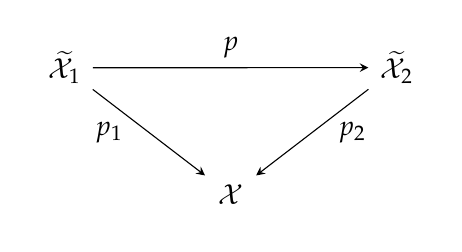
\begin{tikzpicture}
	\matrix (m) [matrix of math nodes,row sep=3em,column sep=4em,minimum width=2em]
	{
		\widetilde{\mathcal X}_1 & &\widetilde{\mathcal X}_2\\ 
		& {\mathcal X}\\};
	\path[-stealth]
	(m-1-1) edge node [above] {$p$} (m-1-3)
	(m-1-1) edge node [left]  {$p_1~~$} (m-2-2)
	(m-1-3) edge node [right] {$~~p_2$} (m-2-2);
	\end{tikzpicture}
	\\
	where $\sX$ is a connected locally connected Hausdorff space and $p_1$, $p_2$ are transitive coverings then $p$ is a transitive covering.
\end{lemma}
\begin{proof}
	For any $x_0 \in \sX$ then there are bijective maps  $G\left(\left.\widetilde\sX_1~\right|\sX \right)\cong p_2^{-1}\left( x_0\right)$, $G\left(\left.\widetilde\sX_2~\right|\sX \right)\cong p_2^{-1}\left( x_0\right)$, so the restriction $\left.p\right|_{p_2^{-1}\left( x_0\right)}$ gives the map $\phi: G\left(\left.\widetilde\sX_2~\right|\sX \right)\to G\left(\left.\widetilde\sX_1~\right|\sX \right)$. The map $\phi$ is  a surjective homomorphism. Let $x_2 \in \widetilde{\mathcal X}_2$ be any point and $x_1 \in \widetilde{\mathcal X}_1$ is such that $p_1\left(x_1 \right) = p_2\left(x_2 \right)$. If $x'_2 = p\left(x_1 \right)$ then there is $g_2 \in G\left(\left.\widetilde\sX_2~\right|\sX \right)$ such that $x_2 = g_2x'_2$. If $g_1 \in G\left(\left.\widetilde\sX_1~\right|\sX \right)$ is such that $g_2 = \phi\left( g_1\right)$ then  $x_2 = p\left( g_1x_1\right)$. So $p$ is a surjective map, and from the Corollary \ref{top_cov_cat_cor} it follows that $p$ is a covering. From 
	$G\left(\left.\widetilde\sX_1~\right|\widetilde\sX_2\right)= \ker \phi$ it turns out that for any $x_2 \in \widetilde{\mathcal X}_2$ the group $G\left(\left.\widetilde\sX_1~\right|\widetilde\sX_2\right)$ transitively acts on $p_2^{-1}\left(x_2\right)$, i.e. $p$ is a transitive covering (cf. Definition \ref{top_transitive_defn}).
\end{proof}

\begin{definition}\label{top_fin_cov_defn}
	Let $\sX$ be a connected locally connected locally compact second-countable Hausdorff space. Let us consider the  category $\mathfrak{FinCov}$-$\sX$ such that
	\begin{itemize}
		\item Objects of  $\mathfrak{FinCov}$-$\sX$ are transitive finite-fold coverings $\widetilde\sX \to \sX$ of $\sX$ where the space $\widetilde\sX$ is connected.
		\item A morphism form $p_1:\widetilde\sX_1 \to \sX$ to $p_2:\widetilde\sX_2 \to \sX$ is a continuous map $p_{12}: \widetilde\sX_1 \to \widetilde\sX_2$ such that $p_{12} \circ p_2 = p_1$.
	\end{itemize}
	We say that $\mathfrak{FinCov}$-$\sX$ is the \textit{finite covering category} of $\sX$.	
\end{definition}
\begin{remark}\label{top_fin_cov_rem}
	We also use the alternative notation in which objects of $\mathfrak{FinCov}$-$\sX$ are covering spaces, i.e. a covering $\widetilde\sX \to \sX$ is replaced with the space $\widetilde\sX$.
\end{remark}
\begin{lemma}\label{top_compliant_covering_lem}
	If $p_1:\widetilde\sX_1 \to \sX$, $p_2:\widetilde\sX_2 \to \sX$ are objects of $\mathfrak{FinCov}$-$\sX$ and $p': \widetilde\sX_1 \to  \widetilde\sX_2$, $p'': \widetilde\sX_1 \to  \widetilde\sX_2$ are morphisms of $\mathfrak{FinCov}$-$\sX$ then there is $g \in 	G\left(\left.\widetilde\sX_2~\right|\sX\right)$ such that
	$$
	p'' =  g \circ p'.
	$$
\end{lemma}
\begin{proof}
	If $\widetilde x_1 \in \widetilde\sX_1$ then from $p_2 \circ p' = p_2 \circ p'' = p_1$ it turns out that $p_2 \circ p'\left(\widetilde x_1\right) = p_2 \circ p''\left(\widetilde x_1\right)$. So there is $g^{\widetilde x_1} \in G\left(\left.\widetilde\sX_2~\right|\sX\right)$ such that $p''\left(\widetilde x_1\right) = g^{\widetilde x_1} p'\left(\widetilde x_1\right)$. Let $\widetilde\sU_1 \subset \widetilde\sX_1$ be an open neighborhood of  $\widetilde x_1$ such that the restriction $\left.p_1\right|_{\widetilde\sU_1}$ is injective, let $\widetilde\sU_2 = p'\left(\widetilde\sU_1 \right)\subset \widetilde\sX_2$ and  $\sU =  p_1\left( \widetilde\sU_1\right)\subset \sX$. For any $\widetilde x'_1 \in \widetilde\sU_1$ one has $p''\left( \widetilde x'_1\right) = g^{\widetilde x_1} p'\left(\widetilde x_1\right)$ it turns out that the map
	\bean
	\widetilde\sU_1 \to G\left(\left.\widetilde\sX_2~\right|\sX\right),\\
	\widetilde x'_1 \mapsto g^{\widetilde x'_1}
	\eean 
	is locally constant. However the space $\widetilde\sX_1$ is connected, so the map $\widetilde x'_1 \mapsto g^{\widetilde x'_1}$ is constant. So there is $g \in 	G\left(\left.\widetilde\sX_2~\right|\sX\right)$ such that $p''\left( \widetilde x'_1\right)  =  g \circ p'\left( \widetilde x'_1\right)$ for all $\widetilde x'_1 \in \widetilde \sX_1$.
	\end{proof} 
\begin{definition}\label{top_pointed_defn}
	If $\sX$ is a set (resp. topological space) and $x_0 \in \sX$ is a base-point then we say that the pair $\left(\sX, x_0 \right)$ is a \textit{pointed set} (resp. \textit{pointed space}). If both $\left(\sX, x_0 \right)$ and $\left(\sY, y_0 \right)$ are pointed spaces and $\varphi: \sX \to \sY$ is such that $\varphi:\left(x_0\right)= y_0$ then we say that $\varphi$ is a \textit{pointed map}. We write
	\be\label{top_pointed_eqn}
	\varphi: \left(\sX, x_0 \right)\to\left(\sY, y_0 \right)
	\ee
\end{definition}
\begin{definition}\label{top_fin_cov_p_defn}
	Let $\left(\sX, x_0 \right)$ be a pointed space such that $\sX$ is a connected locally connected locally compact second-countable Hausdorff space. Let us consider the  category $\mathfrak{FinCov}$-$\left( \sX, x_0\right) $ such that
	\begin{itemize}
		\item Objects of  $\mathfrak{FinCov}$-$\left( \sX, x_0\right)$ are transitive finite-fold coverings $\left( \widetilde\sX, \widetilde x_0\right)  \to \left( \sX, x_0\right)$ of $\sX$ preserving base-points.
		\item A morphism form $p_1:\left( \widetilde\sX_1, \widetilde x^1_0\right)\to \left( \sX, x_0\right)$ to $p_2:\left( \widetilde\sX_2, \widetilde x^2_0\right)\to \left( \sX, x_0\right)$ is a preserving base-points continuous map $p: \widetilde\sX_1 \to \widetilde\sX_2$ such that $p \circ p_1 = p_2$.
	\end{itemize}
	We say that $\mathfrak{FinCov}$-$\left( \sX, x_0\right)$ is the \textit{topological pointed finite covering category} of $\left( \sX, x_0\right)$.  
\end{definition}
\begin{remark}
	The category $\mathfrak{FinCov}$-$\left( \sX, x_0\right)$ is a subcategory of  $\mathfrak{FinCov}$-$\sX$.
\end{remark}
\begin{remark}
	If both $p_1:\left( \widetilde\sX_1, \widetilde x^1_0\right)\to \left( \sX, x_0\right)$ and  $p_2:\left( \widetilde\sX_2, \widetilde x^2_0\right)\to \left( \sX, x_0\right)$ are objects of $\mathfrak{FinCov}$-$\left( \sX, x_0\right)$ then there in no more then one morphism from $p_1$ to $p_2$.
\end{remark}


\begin{lemma}\label{top_fin_int_lem}
	If an indexed family of sets $\left\{\sU_\al\right\}_{\al \in \mathscr A}$ of topological space $\sX$ is {locally finite} (cf. Definition \ref{top_loc_fin_defn}) and subspace $\sY$ of $\sX$ is compact then there is finitely many $\al$ such that  $\sU_\al \cap \sY \neq \emptyset$. 
\end{lemma}
\begin{proof}
	Denote by 
	$$
	\La = \left\{\al \in \mathscr A~|~ \sU_\al \cap \sY \neq \emptyset\right\}
	$$
	and for any $\al \in \La$ we select $x_\a \in \sU_\al \cap \sY$. If $\La$ is not finite then since $\sY$ is compact then there is an infinite directed subset $\La' \subset \La$ such that the net $\left\{x_\a \right\}_{\a \in \La'}$ is convergent. If $y = \lim_{\a \in \La'}a_\a$ then any neighborhood of $y$ contains infinitely intersects with infinitely many sets $\sU_\al$. A contradiction with the Definition \ref{top_loc_fin_defn}.
\end{proof}

\begin{lemma}\label{fin_comp_lin_lem}
	Suppose $\sX$ is a locally compact connected locally connected Lindel\"{o}f Hausdorff space. Then for any $x_0 \in \mathcal X$ there is a finite or countable sequence $\sU_1 \subsetneqq  ...\subsetneqq \sU_n\subsetneqq ...$ of connected open subsets of $\sX$ such that
	\begin{itemize}
		\item $x_0 \in \sU_1$.
		\item  For any $n \in \N$ the closure of $\sU_n$ is compact.
		\item $\cup~ \sU_n = \sX$.
	\end{itemize} 
\end{lemma}
\begin{proof}
	The space $\sX$ is a locally compact, so for any point there is an open neighborhood $\sV_x$ such that the closure of $\sV_x$ is compact. Moreover one can assume that $\sV_x$ is connected since $\sX$ is locally connected. The space is $\sX$ is  Lindel\"{o}f, so there is a finite or countable set $\left\{\sV_\la \right\}_{\la \in \La}$ of connected open subspaces of $\sX$ such that the closure of $\sV_\la$ is compact for all $\la \in \La$. Let us define a finite or countable sequence $\sU_1 \subsetneqq  ...\subsetneqq \sU_n\subsetneqq ...$ by induction.
	\begin{enumerate}
		\item Let us select a $\la_0 \in \La$ such that $x_0 \in \sV_{\la_0}$, and let $\sU_1 = \sV_{\la_0}$.
		\item If $\sU_n$ is already defined then we looking for $\sV_\la$ such that
		\be\label{seqvu_eqn}
		\sV_\la \not\subset \sU_n;\quad
		\sV_\la \cap \sU_n \neq \emptyset.
		\ee
		It there is no $\sV_\la$ which satisfies to \eqref{seqvu_eqn} then the sequence is competed. Otherwise one sets $\sU_{n+1}= \sU_n \cup \sV_\la$.
	\end{enumerate} 
	Clearly that for every $n \in \N$ the set $ \sU_n$ is an open connected and have the compact closure. If  $\sX \neq \cup~ \sU_n$ then 
	$$
	\sX  = \cup ~\sU_n \bigsqcup \cup_{\la \in \La_0} \sV_\la; \text{ where } \sV_\la \bigcap \cup ~\sU_n = \emptyset; ~~ \forall \la \in \La_0,
	$$ 
	i.e. $\sX$ is not connected. So one has $\sX = \cup~ \sU_n$.
\end{proof}


\begin{lemma}\label{top_fin_comp_lin_cov_lem}
	Let $\mathcal X$ be a connected locally connected locally compact Hausdorff Lindel\"{o}f space. Suppose that  $\widetilde{\mathcal X}$ is a topological space with the action $G \times \widetilde{\mathcal X}$ of the finite group $G$. Let $p : \widetilde{\mathcal X} \to {\mathcal X}$ be a $G$-invariant (it means $g \circ p = p \circ g; \quad \forall g \in G$) surjective continuous map. Suppose also that if $G_{\widetilde{x}}= \left\{g \in G~|~g\widetilde{x}= \widetilde{x}  \right\}$ then $\cap_{\widetilde{x}\in \widetilde{   \sX}} G_{\widetilde{x}}$ is trivial.   Then for any $x_0 \in \mathcal X$ there is  a  finite or countable sequence $\sU_1 \subsetneqq  ...\subsetneqq \sU_n\subsetneqq ...$ of connected open subsets of $\sX$ such that
	\begin{enumerate}
		\item[(i)] $x_0 \in \sU_1$.
		\item[(ii)]  For any $n \in \N$ the closure of $\sU_n$ is compact.
		\item[(iii)] $\cup~ \sU_n = \sX$.
		\item[(iv)] The space $p^{-1}\left( \sU_n\right)$ is connected for any $n \in \N$.
		\item[(v)] For any $n \in \N$ the subgroup $G_n$ of $G$ given by
		$$
		G_n = \bigcap_{\widetilde{x}\subset p^{-1}\left(\sU_n \right) }G_{\widetilde{x}};
		$$
		is trivial.
	\end{enumerate}  
\end{lemma}
\begin{proof}
	(i)-(iii) From the Lemma \ref{fin_comp_lin_lem} it follows that there is a  finite or countable sequence $\sU_1 \subsetneqq  ...\subsetneqq \sU_n\subsetneqq ...$ of connected open subsets of $\sX$ such that conditions (i)-(iii) holds.\\
	(iv)
	For any $n \in \N$ we suppose that $\widetilde{\sU}_n \subset \widetilde{\sX}$ is a connected component of $p^{-1}\left( {\sU}_n\right)$ and denote by 
	$$
	H_n = \left\{g \in G~|~ g \widetilde{\sU}_n= \widetilde{\sU}_n\right\}
	$$
	There is nondecreasing sequence of subgroups
	$$
	H_1 \subseteq ...\subseteq H_n \subseteq ...
	$$
	such that $\cup_{n = 1}^\infty H_n = G$. Since the group $G$ is finite there is $m \in \N$ such that $H_n = G$ for any $n \ge m$. So the finite or countable subsequence $\sU_m \subsetneqq  ...\subsetneqq \sU_k\subsetneqq ...$ of $\sU_1 \subsetneqq  ...\subsetneqq \sU_n\subsetneqq ...$ satisfies to the condition (iv).\\
	(v) There is a decreasing sequence of  subgroups
	$$
	G_1 \supseteq ... \supseteq G_n \supset ...
	$$
	The intersection  $\cap_{\widetilde{x}\in \widetilde{   \sX}} G_{\widetilde{x}}$ is trivial, hence the intersection $\cap ~ G_n$ is also trivial. However $G$ is finite, so there is $s \in \N$ such that $G_n = G$ for any $n \ge s$. So the finite or countable subsequence $\sU_s \subsetneqq  ...\subsetneqq \sU_r\subsetneqq ...$ of $\sU_1 \subsetneqq  ...\subsetneqq \sU_n\subsetneqq ...$ satisfies to the condition (v).
\end{proof}

\begin{lemma}\label{top_conn_cov_lem}
	Let $\sX$ be a  connected locally connected space, and let $\sU \subset \sX$ be a connected open subspace. If $p:	\widetilde{   \mathcal X } \to \mathcal X$ is a transitive covering, such that such that the space $\widetilde{\sU} = p^{-1}\left(\sU \right)$ is connected then the restriction $p|_{\widetilde{\sU}}: \widetilde{\sU}\to {\sU}$ is a transitive covering. Moreover  the map
	\be\label{top_res_iso_eqn}
	\begin{split}
		G\left( \widetilde{   \mathcal X }~|~\sX\right)\to G\left( \widetilde{   \mathcal U }~|~\sU\right),\\
		g \mapsto g|_{\widetilde{\sU}}
	\end{split}
	\ee
	is the isomorphism of groups.
\end{lemma}
\begin{proof}
	Clearly $p|_{\widetilde{\sU}}: \widetilde{\sU}\to {\sU}$ is a transitive covering. Let $x_0 \in \sU$ be any point. If $\widetilde{x}_0\in \widetilde{\sU}$ is such that $p\left( \widetilde{x}_0\right) = x_0$. Since $p$ is transitive for any $g_{\mathcal U} \in G\left( \widetilde{   \mathcal U }~|~\sU\right)$ there is the unique $g \in G\left( \widetilde{   \mathcal X }~|~\sX\right)$ such that $g_{\mathcal U}\widetilde{x}_0 = g\widetilde{x}_0$. Moreover there is an open neighborhood $\widetilde{   \mathcal V } \subset \widetilde{   \mathcal V }$ of $\widetilde{x}_0$ such that $g_{\mathcal U}\widetilde{x} = g\widetilde{x}$ for every  $\widetilde{x}\in \widetilde{\sV}$. It turns out that the set
	$$
	\widetilde{\sU}_g = \left\{\widetilde{x}\in \widetilde{\sU}~|~g_{\mathcal U}\widetilde{x} = g\widetilde{x}\right\}
	$$
	is open for any $g \in G$. Otherwise from $\widetilde{\sU}= \sqcup_{g\in G} \widetilde{\sU}_g$ and taking into account that $\widetilde{\sU}$ one has two options
	\begin{itemize}
		\item $\widetilde{\sU}_g= \widetilde{\sU}$.
		\item $\widetilde{\sU}_g = \emptyset$.
	\end{itemize}
	The following group homomorphism
	\bean
	G\left( \widetilde{   \mathcal U }~|~\sU\right)\to	G\left( \widetilde{   \mathcal X }~|~\sX\right),\\
	g_{\sU} \mapsto g \quad\text{ where }\quad \widetilde{\sU}_g= \widetilde{\sU}
	\eean
	is inverse to \eqref{top_res_iso_eqn}
\end{proof}









\begin{empt}\label{fin_comp_lin_empt}
	If consider the situation of the Lemma \ref{fin_comp_lin_lem}, then from the Remark \ref{top_loc_comp_para_rem} and the Theorem \ref{top_part_u_thm} it turns out that 
	there is a partition of unity 
	$$
	\sum_{ \la\in \La}f_\la
	$$
	dominated by  $\left\{\sV_\la \right\}_{\la \in \La}$. From the proof of the Lemma \ref{fin_comp_lin_lem} it turns out that for any $n \in \N$ there is a finite subset $\La_n \subset \La$ such that $\sU_n = \cup_{\la \in \La_n}\sV_\la$. If 
	\be\label{fin_comp_lin_eqn}
	f_n = \sum_{ \la \in \La_n}f_\la
	\ee
	then there is a point-wise limit $1_{C_b\left(\sX \right) } = \lim_{n\to \infty}f_n$.
\end{empt}



\section{Lift and descent}\label{top_lif_desc_sec}
\paragraph*{}
Let $\sX$ be a locally compact Hausdorff space called the base space; and for each $x$ in $\sX$, let $A_x$ be a (complex) Banach space. Let us consider a continuity structure $\sF$ for $\sX$ {and the} $\left\{A_x\right\}_{x \in \sX}$ (cf. Definition \ref{op_vect_field_empt}). Denote by $C\left(\sX, \left\{A_x\right\}, \sF \right)$ the $C_b\left(\sX \right)$-module of continuous sections (with respect to) $\sF$ vector fields. 

\begin{lemma}\label{top_c_cont_str}
	\begin{enumerate}
		\item[(i)] If $\sF$ is a continuity structure  for $\sX$ {and the} $\left\{A_x\right\}$ (cf. Definition \ref{op_vect_field_empt}), then $C\left(\sX, \left\{A_x\right\}, \sF \right)$ is a continuity structure  for $\sX$ {and the} $\left\{A_x\right\}$.
		\item[(ii)]
		\be
		C\left(\sX, \left\{A_x\right\}, \sF \right)= C\left(\sX, \left\{A_x\right\}, C\left(\sX, \left\{A_x\right\}, \sF \right) \right)
		\ee
	\end{enumerate}
\end{lemma} 
\begin{proof}
	(i) One needs check conditions (a), (b) of the Definition \ref{op_fields_defn}.
	\begin{enumerate}
		\item [(a)] Follows from the Lemma \ref{op_cont_con_lem}.
		\item[(b)] Follows from the inclusion $\sF \subset C\left(\sX, \left\{A_x\right\}, \sF \right)$.
	\end{enumerate}
	(ii) From $\sF \subset C\left(\sX, \left\{A_x\right\}, \sF \right)$ it follows that $$C\left(\sX, \left\{A_x\right\}, \sF \right)\subset C\left(\sX, \left\{A_x\right\}, C\left(\sX, \left\{A_x\right\}, \sF \right)\right).$$
	Let $a \in C\left(\sX, \left\{A_x\right\}, C\left(\sX, \left\{A_x\right\}, \sF \right)\right) $, let $x_0 \in \sX$ and $\eps > 0$. There is an open neighborhood  $\sU'$ of $x_0$ and $a' \in C\left(\sX, \left\{A_x\right\}, \sF \right)$ such that $\left\|a\left(x \right)  - a'\left(x \right)\right\| < \frac{\eps}{2}$ for all $x \in \sU'$. Otherwise there is an open neighborhood  $\sU'$ of $x_0$ and $a'' \in \sF$ such that $\left\|a'\left(x \right)  - a''\left(x \right)\right\| < \frac{\eps}{2}$ for every $x \in \sU''$. It follows that $\left\|a\left(x \right)  - a''\left(x \right)\right\| < \eps$ for every $x \in \sU'\cap\sU''$, hence one has $a \in C\left(\sX, \left\{A_x\right\}, \sF \right)$. In result we conclude that
	$$ C\left(\sX, \left\{A_x\right\}, C\left(\sX, \left\{A_x\right\}, \sF \right)\right)\subset C\left(\sX, \left\{A_x\right\}, \sF \right).$$
\end{proof} 

Let us define $\left\|\cdot\right\|: C\left(\sX, \left\{A_x\right\},\sF\right)\to \left[0, \infty\right)$ given by
\be\label{top_norm_eqn}
\left\|a\right\|= \sup_{x \in \sX}\left\|a_x\right\|
\ee
\begin{definition}\label{top_s_bounded_defn}
	The space $C_b\left(\sX, \left\{A_x\right\},\sF\right)$ given by
	\be\label{top_s_bounded_eqn}
	C_b\left(\sX, \left\{A_x\right\},\sF\right) = \left\{\left.a \in C\left(\sX, \left\{A_x\right\},\sF\right)\right|\left\|a\right\| < \infty\right\}.
	\ee
	is said to be the \textit{space of bounded continuous sections}.
\end{definition}
\begin{lemma}\label{top_bounded_norm_lem}
	One has
	\be\nonumber
	a \in C_b\left(\sX, \left\{A_x\right\},\sF\right) \Rightarrow \left( x \mapsto \left\|a\left(x \right) \right\| \right) \in C_b\left(\sX \right) 
	\ee
\end{lemma}
\begin{proof}
	From the Lemma 	\ref{op_cont_con_lem} it follows that the map $x \mapsto \left\|a\left(x \right) \right\|$ is continuous, from \eqref{top_s_bounded_eqn} it follows that $x \mapsto \left\|a\left(x \right) \right\|$ is bounded.
\end{proof}
\begin{definition}\label{top_cc_supp_defn}
	If $a\in  C\left(\sX, \left\{A_x\right\}, C\left(\sX, \left\{A_x\right\}, \sF \right)\right)\subset C\left(\sX, \left\{A_x\right\}, \sF \right)$ is presented by the family
	If $\left\{a_x \in A_x\right\}$ then the closure of $\left\{\left. x \in \sX~\right|\left\| a_x\right\| > 0\right\}$ is said to be the \textit{support} of $a$. We write
\be\label{top_support_eqn}
\supp a  \stackrel{\text{def}}{=} \text{ the closure of }\left\{\left. x \in \sX~\right|\left\| a_x\right\| > 0\right\}.
\ee
\end{definition}
\begin{definition}\label{top_cc_c0_defn}
	The $C_b\left(\widetilde{\sX}\right) $-module 
	\be
	C_c\left(\sX, \left\{A_x\right\}, \sF \right) = \left\{\left.a \in C_b\left(\sX, \left\{A_x\right\}, \sF \right)~\right| \supp\left( a\right) \text{ is compact } \right\}
	\ee
	is said to be the \textit{compactly supported submodule}. The norm completion of $C_c\left(\sX, \left\{A_x\right\}, \sF \right)$ is said to be \textit{converging to zero submodule} and we denote it by $C_0\left(\sX, \left\{A_x\right\}, \sF \right)$. We also use the following notation
	\bea
	\label{top_cc_eqn}
	C_c\left(A \right) = C_c\left(\sX, \left\{A_x\right\}, A \right),\\
	\label{top_c0_eqn}
	C_0\left(A \right) = C_0\left(\sX, \left\{A_x\right\}, A \right),\\
	\label{top_cb_eqn}
	C_b\left(A \right) = C_b\left(\sX, \left\{A_x\right\}, A \right),\\
	\label{top_c_eqn}
	C\left(A \right) = C\left(\sX, \left\{A_x\right\}, A \right).
	\eea
	
\end{definition}
\begin{remark}
	The Definition \ref{top_cc_c0_defn} is compliant with \ref{ctr_crooss_alg_empt}.
\end{remark}

\begin{empt}
For any $a \in C\left(\sX, \left\{A_x\right\}, \sF \right)$ denote by 
\bea
\label{top_norm_a_eqn}
\text{norm}_a \in C_b\left(\sX \right), \quad x \mapsto \left\|a\left(x \right) \right\|;\\
\label{top_res_eqn}
\left.C_0\left(\sX, \left\{A_x\right\}, \sF  \right) \right|_{\sU}\stackrel{\text{def}}{=}\left\{\left.a \in C_0\left(\sX, \left\{A_x\right\}, \sF  \right)~\right|~ \supp a \subset \sU \right\}.
\eea
\end{empt}
\begin{remark}
If $C_0\left(\sX, \left\{A_x\right\}, \sF  \right)$ is a $C^*$-algebra with continuous  trace then the notation \eqref{top_res_eqn} complies  with \eqref{open_ideal_eqn} (cf. the Lemma \ref{top_res_eqn} below).
\end{remark}
\begin{lemma}\label{top_multiple_a_lem}
	If $\sF$ is a continuity structure  for $\sX$ {and the} $\left\{A_x\right\}_{x \in \sX}$ (cf. Definition \ref{op_vect_field_empt}), and let $a \in C_b\left( \sX, \left\{A_x\right\}, \sF\right)$. Suppose $\mathrm{norm}_a$ is multiple of $f \in C_b\left(\sX \right)$ (cf. Definition \ref{top_multiple_defn}). Let $\sU = \left\{\left.x \in \sX~\right| f\left( x\right) \neq 0 \right\}$. If  $\left\{b_x\in A_x\right\}_{x \in \sX}$ is the family given by
	\be\label{top_multiple_a_eqn}
	b_x = \left\{\begin{array}{c l}
		\frac{a\left( x\right) }{f\left( x\right)}  & x \in \sU\\
		0 & x \notin \sU\\
	\end{array}\right|
	\ee
	then there is $b \in C_b\left( \sX, \left\{A_x\right\}, \sF\right)$ such that $b\left(x \right) = b_x$ for any $x \in \sX$. Moreover
	\be\label{top_multiple_na_eqn}
	\left\| 	b_x\right\|  = \left\{\begin{array}{c l}
		\frac{\left\| a\left( x\right)\right\|  }{f\left( x\right)}  & x \in \sU\\
		0 & x \notin \sU\\
	\end{array}\right|
	\ee
\end{lemma}
\begin{proof}
	Firstly we proof $\left\{b_x\right\}\in C\left( \sX, \left\{A_x\right\},  C_0\left( \sX, \left\{A_x\right\}, \sF\right)\right)$. 
	For any  $x_0 \in \sX$ then we consider two cases:
	\begin{enumerate}
		\item [(i)] $x_0 \in \sU$. The function
		Consider $f_{x_0}\in C_c\left( \sX\right) $ such that $f_{x_0}\left(\sX \right) = \left[0,1\right]$ supp $f_{x_0}\subset \supp f$ and there is an open neighborhood $\sV$ of $x_0$ which satisfies to $f_{x_0}\left(\sV \right) = \left\{1\right\}$. From the Lemma \ref{top_multiple_lem} it turns out $f_{x_0}$ is a multiple of $f$, i.e. there is $f' \in C_b\left(\sX \right)$ such that $f_{x_0} = f'f$. If $a_{f'} = f'a\in C_b\left( \sX, \left\{A_x\right\}, \sF\right)$ then $a_{f'}\left(x \right) = b_x$ for any $x \in \sV$.
		\item [(ii)] $x_0 \notin \sU$. From the Lemma \ref{top_multiple_lem} it turns that out for any $\eps > 0$  there is an open  neighborhood $\mathcal W$ of $x_0$ such that $\left\|b_x \right\|< \eps$ for any $x \in \mathcal{W}$. 
	\end{enumerate}
	If $\mathfrak{div}\left( \mathrm{norm}_a,f\right)$ is given by \eqref{top_multiple_eqn} then 
	$$
	\left\|b_x \right\| \le \left\|\mathfrak{div}\left( \mathrm{norm}_a,f\right) \right\| \quad \forall x \in \sX.
	$$
	The equation \eqref{top_multiple_na_eqn} follows from \eqref{top_multiple_a_eqn}.
\end{proof}

\begin{definition}\label{top_multiple_a_defn}
	In the situation of the Lemma \ref{top_multiple_a_lem}
	we write
	\be\label{top_multiple_ad_eqn}
	\begin{split}
		\mathfrak{div}\left( a,f\right)\stackrel{\text{def}}{=} b \in C_b\left( \sX, \left\{A_x\right\}, \sF\right).
	\end{split}
	\ee
\end{definition}


\begin{lemma}\label{top_norm_c0cc_lem}
	Following conditions hold
	\bea
	\label{top_ccn_eqn}
	C_c\left(A \right) = \left\{\left.a \in 	C_b\left(A \right)~\right| ~\mathrm{norm}_a \in 	C_c\left(\sX\right)\right\},\\
	\label{top_cc0_eqn}
	C_0\left(A \right) = \left\{\left.a \in 	C_b\left(A \right)~\right| ~\mathrm{norm}_a \in 	C_0\left(\sX\right)\right\}
	\eea
	(cf. Equations \eqref{top_norm_a_eqn}, \eqref{top_cb_eqn}-\eqref{top_c0_eqn})
\end{lemma}
\begin{proof}
	The equation \eqref{top_ccn_eqn} is evident. If $a \in C_0\left( A\right)$ then there is a $C^*$-norm convergent net $\left\{a_\a \in 	C_c\left(A \right)\right\}_{\a \in \mathscr A}$ such that $a = \lim a_\a$. For any $\a, \bt \in \mathscr A$ one has
	\be\label{top_ab_norm_eqn}
	\left\|\text{norm}_{a_\a} - \text{norm}_{a_\bt} \right\|\le \left\|{a_\a} - {a_\bt} \right\|.
	\ee
	From \eqref{top_ab_norm_eqn} it turns out that the net $\left\{\text{norm}_{a_\a}\right\}$ is convergent. From $\text{norm}_{a_\a} \in C_c\left( \sX\right)$ it turns out $\lim \text{norm}_{a_\a} \in C_0\left(\sX \right)$, otherwise one has $\text{norm}_{a}=\lim_\a \text{norm}_{a_\a}$. Conversely let $a \in C_b\left( A\right)$ be such that $\mathrm{norm}_a \in 	C_0\left(\sX\right)$. If $F_\eps$ is given by \eqref{top_f_eps_eqn} and $a_\eps \in C_b\left( A\right)$ is such that $a_\eps  = F_\eps\left(\mathrm{norm}_a \right)a$ then from  \eqref{top_f_eps_n_eqn} and \eqref{top_f0_eps_n_eqn}   it turns out that
	\bea \label{top_f_eps_na_eqn}
	\left\| a_\eps  - a \right\| \le \eps,\\
	\label{top_f0_eps_na_eqn}
	\supp a_\eps \text{ is compact}. 
	\eea
	From \eqref{top_f_eps_na_eqn} and \eqref{top_f0_eps_na_eqn} it turns out $a = \lim_{\eps \to 0}a_\eps$  and $a_\eps \in C_c\left( A\right)$ respectively. Taking into account the Definition \ref{top_cc_c0_defn} one has $a \in C_0\left(A\right)$.  
\end{proof}
\begin{corollary}\label{top_c0_cont_str_cor}
	One has
	\be\label{top_c0_cont_strc_eqn}
	\sX \mathrm{~is~compact~} \Rightarrow	C_c\left(A \right)= 	C_0\left(A \right)= 	C_b\left(A \right)= 	C\left(A \right).
	\ee	
\end{corollary}
\begin{lemma}\label{top_c0_cont_str_lem}
	\begin{enumerate}
		\item[(i)] If $\sF$ is a continuity structure  for $\sX$ {and the} $\left\{A_x\right\}$ (cf. Definition \ref{op_vect_field_empt}), then all of $C_c\left(\sX, \left\{A_x\right\}, \sF \right)$, $C_0\left(\sX, \left\{A_x\right\}, \sF \right)$ and $C_b\left(\sX, \left\{A_x\right\}, \sF \right)$ are a continuity structures  for $\sX$ {and the} $\left\{A_x\right\}$.
		\item[(ii)]
		\be\label{top_c0_cont_str_eqn}
		\begin{split}
			C\left(\sX, \left\{A_x\right\}, \sF \right)= C\left(\sX, \left\{A_x\right\}, C_c\left(\sX, \left\{A_x\right\}, \sF \right) \right)=\\
			C\left(\sX, \left\{A_x\right\}, C_0\left(\sX, \left\{A_x\right\}, \sF \right) \right)= C\left(\sX, \left\{A_x\right\}, C_b\left(\sX, \left\{A_x\right\}, \sF \right) \right)
		\end{split}
		\ee
	\end{enumerate}
\end{lemma}

\begin{proof}
	For any $x_0$ denote by $f_{x_0}\in C_c\left( \sX\right) $ such that $f_{x_0}\left(\sX \right) = \left[0,1\right]$ and there is an open neighborhood $\sU$ of $x_0$ which satisfies to $f_{x_0}\left(\sU \right) = \left\{1\right\}$.
	(i) One needs check conditions (a), (b) of the Definition \ref{op_fields_defn}.
	\begin{enumerate}
		\item [(a)] Follows from the Lemma \ref{op_cont_con_lem}.
		\item[(b)] For any $a \in \sF$ one has $f_{x_0} a \in  C_c\left(\sX, \left\{A_x\right\}, \sF \right)$, and from $f_{x_0}\left( x_0\right) =1$ it turns out
		\bean
		A=	\left\{\left. a_x \in A_x\right|\exists a \in \sF \quad a_x = a\left( x\right)  \right\}\subset \\ \subset A_c=	\left\{\left. a_x \in A_x\right|\exists a \in C_c\left(\sX, \left\{A_x\right\}, \sF \right) \quad a_x = a\left( x\right)  \right\}.
		\eean
		Since $A$ is dense in $A_x$, so $A_c$ is dense in $A_x$. If
		\bean
		A_0=	\left\{\left. a_x \in A_x\right|\exists a \in C_0\left(\sX, \left\{A_x\right\}, \sF \right) \quad a_x = a\left( x\right)  \right\},\\
		A_b=	\left\{\left. a_x \in A_x\right|\exists a \in C_b\left(\sX, \left\{A_x\right\}, \sF \right) \quad a_x = a\left( x\right)  \right\}
		\eean 
		then from
		$$
		A \subset A_c \subset A_0 \subset A_b \subset A_x
		$$
		it turns out that $A_0$ and $A_b$ are dense in $A_x$.
	\end{enumerate}
	(ii) From the inclusions
	$$
	C_c\left(\sX, \left\{A_x\right\}, \sF \right) \subset C_0\left(\sX, \left\{A_x\right\}, \sF \right) \subset C_b\left(\sX, \left\{A_x\right\}, \sF \right) \subset C\left(\sX, \left\{A_x\right\}, \sF \right).
	$$
	
	and the equation \eqref{top_c0_cont_str_eqn} it follows that 
	\be\label{top_c0_cont_str_j_lem}
	\begin{split}
		C\left(\sX, \left\{A_x\right\}, C_c\left(\sX, \left\{A_x\right\}, \sF \right) \right)\subset 	C\left(\sX, \left\{A_x\right\}, C_0\left(\sX, \left\{A_x\right\}, \sF \right)\right)\subset \\ \subset  
		C\left(\sX, \left\{A_x\right\}, C_b\left(\sX, \left\{A_x\right\}, \sF \right) \right)\subset 	C\left(\sX, \left\{A_x\right\}, \sF \right).
	\end{split}
	\ee 
	Let $a \in C\left(\sX, \left\{A_x\right\}, C\left(\sX, \left\{A_x\right\}, \sF \right)\right) $, let $x_0 \in \sX$ and $\eps > 0$. There is an open neighborhood  $\sU'$ of $x_0$ and $a' \in C\left(\sX, \left\{A_x\right\}, \sF \right)$ such that $\left\|a\left(x \right)  - a'\left(x \right)\right\| < \eps$ for all $x \in \sU'$. Otherwise  $a'' = f_{x_0}a' \in  C_c\left(\sX, \left\{A_x\right\}, \sF \right)$ and one has $\left\|a\left(x \right)  - a''\left(x \right)\right\| < \eps$ for all $x \in \sU \cap\sU'$. It follows that $a \in 	C\left(\sX, \left\{A_x\right\}, C_c\left(\sX, \left\{A_x\right\}, \sF \right) \right)$, so one has
	$$
	C\left(\sX, \left\{A_x\right\}, \sF \right) \subset C\left(\sX, \left\{A_x\right\}, C_c\left(\sX, \left\{A_x\right\}, \sF \right) \right),
	$$
	and taking into account \eqref{top_c0_cont_str_j_lem} one  obtains \eqref{top_c0_cont_str_eqn} 
\end{proof} 
\begin{corollary}\label{top_c0_cont_str_f_cor}
	Following conditions hold:
	\be\label{top_c0_cont_str_cor_eqn}
	\begin{split}
		C_c\left(\sX, \left\{A_x\right\}_{x \in \sX}, C_c\left(\sX, \left\{A_x\right\}_{x \in \sX}, \sF  \right)  \right)=\\= 	C_c\left(\sX, \left\{A_x\right\}_{x \in \sX}, C_0\left(\sX, \left\{A_x\right\}_{x \in \sX}, \sF  \right)  \right)=\\=C_c\left(\sX, \left\{A_x\right\}_{x \in \sX}, C_b\left(\sX, \left\{A_x\right\}_{x \in \sX}, \sF  \right)  \right)=\\= 	C_c\left(\sX, \left\{A_x\right\}_{x \in \sX}, C\left(\sX, \left\{A_x\right\}_{x \in \sX}, \sF  \right)  \right)=C_c\left(\sX, \left\{A_x\right\}_{x \in \sX}, \sF  \right),\\
		C_0\left(\sX, \left\{A_x\right\}_{x \in \sX}, C_c\left(\sX, \left\{A_x\right\}_{x \in \sX}, \sF  \right)  \right)=\\= 	C_0\left(\sX, \left\{A_x\right\}_{x \in \sX}, C_0\left(\sX, \left\{A_x\right\}_{x \in \sX}, \sF  \right)  \right)=\\=C_0\left(\sX, \left\{A_x\right\}_{x \in \sX}, C_b\left(\sX, \left\{A_x\right\}_{x \in \sX}, \sF  \right)  \right)=\\= 	C_0\left(\sX, \left\{A_x\right\}_{x \in \sX}, C\left(\sX, \left\{A_x\right\}_{x \in \sX}, \sF  \right)  \right)=C_0\left(\sX, \left\{A_x\right\}_{x \in \sX}, \sF  \right),\\
		C_b\left(\sX, \left\{A_x\right\}_{x \in \sX}, C_c\left(\sX, \left\{A_x\right\}_{x \in \sX}, \sF  \right)  \right)=\\= 	C_b\left(\sX, \left\{A_x\right\}_{x \in \sX}, C_0\left(\sX, \left\{A_x\right\}_{x \in \sX}, \sF  \right)  \right)=\\=C_b\left(\sX, \left\{A_x\right\}_{x \in \sX}, C_b\left(\sX, \left\{A_x\right\}_{x \in \sX}, \sF  \right)  \right)=\\= 	C_b\left(\sX, \left\{A_x\right\}_{x \in \sX}, C\left(\sX, \left\{A_x\right\}_{x \in \sX}, \sF  \right)  \right)=C_b\left(\sX, \left\{A_x\right\}_{x \in \sX}, \sF  \right).
	\end{split}
	\ee
\end{corollary}

\begin{lemma}
	If $\sF$ is a continuity structure $\sF$ for $\sX$ {and the} $\left\{A_x\right\}$ such that 
	$$
	\mathrm{norm}_a \in C_0\left(\sX \right) \quad \forall a \in \sF
	$$
	Then the space $C_0\left(\sX \right)\sF$ is dense in 	$C_0\left(\sX, \left\{A_x\right\}, \sF \right)$. 
\end{lemma}
\begin{proof}
	Suppose $a \in C_0\left(\sX, \left\{A_x\right\}, \sF \right)$ and $\eps > 0$. If $F_\eps$ is given by \eqref{top_f_eps_eqn} and $$
	a_\eps \stackrel{\text{def}}{=}F_{\eps}\left(\text{norm}_a \right) a
	$$ then one has
	\bea
	\left\| a - a_\eps\right\| \le \frac{\eps}{2},\\
	\supp  a_\eps \text{ is compact}.
	\eea
	For any $x \in \supp  a_\eps$ we select $a^x \in \sF$ and an open neighborhood  $\sU_x$ of $x$ such that $\left\| a\left(y \right)  - a^x_y\right\|< \frac{\eps}{2}$ for all $y \in \sU_x$.  Since $\supp  a_\eps$ is compact there is a finite set $\left\{ {   \mathcal U }_{{x}_1}, ...,  {   \mathcal U }_{{x}_n}\right\} \subset  \left\{ {   \mathcal U }_{{x}}\right\}_{{x }\in {   \mathcal U }}$ such that ${   \mathcal U } = \cup_{j=1}^n {   \mathcal U }_{{x}_j}$. Write $\left\{ {   \mathcal U }_{1}, ...,  {   \mathcal U }_{n}\right\}\stackrel{\text{def}}{=}\left\{ {   \mathcal U }_{{x}_1}, ...,  {   \mathcal U }_{{x}_n}\right\}$ and $\left\{ a_{1}, ...,  a_{n}\right\}\stackrel{\text{def}}{=}\left\{ {  a}^{{x}_1}, ...,  {a}^{{x}_n}\right\}$.
	There is $f_1, ..., f_n \in C_c\left(\sX \right)$ such that
	\bean
	\sum_{j=1}^n f_j\left( x \right) =1 \quad \forall x \in \supp a_\eps,\\
	\supp f_j \subset \sU_j 
	\eean 
	If follows that
	\bean
	\sum_{j=1}^n f_j  a_j \in C_0\left(\sX\right)\sF,\\
	\left\| \sum_{j=1}^n f_j  a_j - a_\eps\right\| \le \frac{\eps}{2}
	\eean 
	and taking into account $\left\| a - a_\eps\right\| \le \frac{\eps}{2}$ one has
	\bean
	\left\| \sum_{j=1}^n f_j  a_j - a\right\| \le \frac{\eps}{2}
	\eean 
\end{proof}
\begin{corollary}\label{top_cl_cc_iso_cor}
	Let $\sF$ be a continuity structure  for $\sX$ {and the} $\left\{A_x\right\}$ such that 
	$$
	\mathrm{norm}_a \in C_0\left(\sX \right) \quad \forall a \in \sF
	$$
	If  $C_0\left(\sX \right)\sF\subset \sF$  and $\sF$ is norm closed then the the natural inclusion $\sF \hookto C_0\left(\sX, \left\{A_x\right\}, \sF \right)$ is the $C_0\left(\sX \right)$-isomorphism
	$$
	\sF \cong C_0\left(\sX, \left\{A_x\right\}, \sF \right).
	$$ 
\end{corollary}

\begin{empt}\label{top_bt_empt}
	Let us select $x \in \sX$. From (ii) of the Definition \ref{ctr_sec_defn} it turns out that the $\C$-space
	$$
	\left\{\left. a_x \in A_x~\right| \exists a \in C_b\left(\sX, \left\{A_x\right\}, \sF \right) \quad a_x = a\left(x \right)  \right\}
	$$
	is dense in $A_x$. So there is the map
	\be\label{top_vp_map}
	\varphi_x:C_b\left(\sX, \left\{A_x\right\}, \sF \right) \to A_x.
	\ee
	Denote by $I_x = \left\{\left.f \in C_b\left(\sX \right)\right|  f\left( x\right)=0  \right\}$, and let $I_x C\left(\sX, \left\{A_x\right\}, \sF \right)$ be a submodule such that 
	$$
	\varphi_x\left( I_x C\left(\sX, \left\{A_x\right\}, \sF \right) \right) = 0.
	$$
	and if 
	\be\label{top_cx_eqn}
	C_x = C\left(\sX, \left\{A_x\right\}, \sF \right)/I_x C_b\left(\sX, \left\{A_x\right\}, \sF \right)
	\ee 
	then there is a $\C$-linear map
	$$
	\phi_x:C_x \to A_x.
	$$
	Let us define a norm on $C_x$ given by
	\be\label{top_cx_norm_eqn}
	\left\|c \right\|_{C_x} = \inf_{\substack{a \in C\left(\sX, \left\{A_x\right\}, \sF \right)  \\ c = a + I_x C\left(\sX, \left\{A_x\right\}, \sF \right)}}\left\|a \right\|
	\ee
	Clearly $\left\|c \right\|_{C_x} \ge \left\|\phi_x\left(c \right)  \right\|$. Let us select a representative $a \in C\left(\sX, \left\{A_x\right\}, \sF \right)$ of $c$. If $\sU_\a$ is a fundamental system of neighborhoods of $x$ then there is a system of continuous functions $\left\{f_\a \in C_c\left( \sX\right) \right\}$ such that
	\bea
	f_\a\left(\sX \right)=\left[0,1\right],\\
	\supp f_\a = \sU_\a,\\
	f_\a\left( x\right) =1.
	\eea
	Since $\text{norm}_a$ is continuous one has
	\bea
	\inf_{\a} \left\|f_\a a\left(x \right)  \right\|=   \left\| a\left(x \right)  \right\|,\\
	\left\|c \right\|_{C_x} = \left\|\phi_x\left(c \right)  \right\|,
	\eea
	i.e. $\phi_x:C_x \to A_x$ is the norm preserving map, and 
	$A_x$ can be defined as the norm completion of $C_x$.
	If $\bt\sX$ is the Stone-\v{C}ech compactification of $\sX$ one can define $A_x$ for any $x \in \bt\sX$. For any $x \in \bt\sX$ there is an ideal $I_x \subset C\left(\bt\sX \right)= C_b\left( \sX\right)$ and similarly to above construction there is the normed space $C_x$. 
\end{empt}
\begin{definition}\label{top_beta_ext_defn}
	Let $\sF$ be a continuity structure  for $\sX$ {and the} $\left\{A_x\right\}_{x\in\sX}$. A family $\left\{\bt A_{\bt x}\right\}_{x\in\bt\sX}$ such that $\bt A_{\bt x}$ is a completion of $C_{ \bt x}$ is said to be the \textit{Stone-\v{C}ech extension} or the $\bt$-\textit{extension} of $\left\{A_x\right\}_{x\in\sX}$.
\end{definition}
For all $x \in \sX$ then clearly $A_x \cong \bt A_{ x}$. For any $a \in  C_b\left(\sX, \left\{A_x\right\}, \sF \right)$ on can define a family
$
\bt\left( a\right) =\left\{ a_{\bt x} \in \bt A_{\bt x}\right\}
$
such that 
\be\label{top_beta_fam_eqn}
a_{\bt x}= \phi_x\left(a + I_{{\bt x}} C_b\left(\sX, \left\{A_x\right\}, \sF \right) \right) 
\ee
From $\text{norm}_a \in C_b\left(\sX \right)$ one has $\text{norm}_{\bt\left( a\right) } \in C\left( \bt\sX\right)$, so the space $\bt\sF$ of families \ref{top_beta_fam_eqn}  is  a continuity structure  for $\bt\sX$ {and the} $\left\{\bt A_{\bt x}\right\}$. Since $\bt\sF$ is norm closed and $\bt\sF$ is compact one has
\be\label{top_bt_f_eqn}
\begin{split}
	\bt\sF = C_c\left(\bt\sX, \left\{\bt A_{\bt x}\right\}_{x\in\bt\sX}, \bt\sF \right)= C_0\left(\bt\sX, \left\{\bt A_{\bt x}\right\}_{x\in\bt\sX}, \bt\sF \right)= \\=C_b\left(\bt\sX, \left\{\bt A_{\bt x}\right\}_{x\in\bt\sX}, \bt\sF \right)= C\left(\bt\sX, \left\{\bt A_{\bt x}\right\}_{x\in\bt\sX}, \bt\sF \right).
\end{split}
\ee
From the equation \eqref{top_beta_fam_eqn} it turns out that for all $\bt x \in \bt\sX$ there is the $\C$-linear map
\be\label{top_vpb_map}
\phi_{ \bt x}:  C_b\left(\sX, \left\{A_x\right\}, \sF \right) \to \bt A_{\bt x}
\ee
such that $\phi_{ \bt x}\left(  C_b\left(\sX, \left\{A_x\right\}, \sF \right)\right) $ is dense in $A_{\bt x}$.
\begin{definition}\label{top_stone_c_defn}
	The continuity structure $\bt\sF$  for $\bt\sX$ {and the} $\left\{\bt A_{\bt x}\right\}$ given by \eqref{top_beta_fam_eqn} is said to be  the \textit{Stone-\v{C}ech extension} or the $\bt$-\textit{extension} of $\sF$.
\end{definition}
\begin{remark}
	From the the construction the family $\bt\left( a\right) =\left\{ a_{\bt x} \in \bt A_{\bt x}\right\}$  uniquely depends on $a \in C_b\left(\sX, \left\{A_x\right\}, \sF \right)$. It turns out that there is the natural $C_b\left(\sX \right)$-isomorphism
	\be\label{top_sf_bt_iso_eqn}
	\bt\sF \cong C_b\left(\sX, \left\{A_x\right\}, \sF \right)
	\ee  
	
\end{remark}


\begin{lemma}\label{top_cb_lem}
	Let $\bt\sF$ be the given by \eqref{top_beta_fam_eqn} continuity structure  for $\bt\sX$ {and the} $\left\{\bt A_{\bt x}\right\}$. If $A \subset \bt\sF$ a norm closed  $C\left(\bt\sX \right)$-submodule which is a continuity structure for   $\bt\sX$ {and the} $\left\{\bt A_{\bt x}\right\}$ then there is the natural isomorphism
	\be\label{top_cb_lem_eqn}
	A \cong C_b\left(\sX, \left\{A_x\right\}, \sF  \right) 
	\ee
\end{lemma}
\begin{proof}
	The inclusion $A \subset \bt\sF$ induces the inclusion $A \subset C_b\left(\bt\sX, \left\{\bt A_{\bt x}\right\}, \bt\sF  \right)$. From the Corollaries \ref{top_c0_cont_str_cor} and \ref{top_cl_cc_iso_cor} it follows that  $A = C_b\left(\bt\sX, \left\{\bt A_{\bt x}\right\}, \bt\sF  \right)$, and taking into account $C_b\left(\bt\sX, \left\{\bt A_{\bt x}\right\}, \bt\sF  \right)\cong C_b\left(\sX, \left\{ A_{x}\right\}, \sF  \right)$ one has \ref{top_cb_lem_eqn}.
\end{proof}
\begin{empt}\label{top_mult_inc_empt}
		Let $\sF$ be a continuity structure  for $\sX$ {and the} $\left\{A_x\right\}_{x\in\sX}$, such that $A_x$ is a $C^*$-algebra for any $x \in \sX$. From \ref{ctr_crooss_alg_empt} it follows that    $C_0\left(   \sX, \left\{A_x\right\}, \sF\right)$ is a $C^*$-algebra. Otherwise from \eqref{top_bt_f_eqn} it turns out that
		$$
		C_b\left(\sX, \left\{ A_{x}\right\}, \sF  \right) = C_0\left(\bt\sX, \left\{ \bt A_{x}\right\}, \sF  \right)
		$$
		and taking into account \ref{ctr_crooss_alg_empt} one concludes that 	$C_b\left(\sX, \left\{ A_{x}\right\}, \sF  \right)$ is a $C^*$-algebra.
\end{empt}
\begin{lemma}\label{top_mult_inc_b_lem}
	In the situation of \ref{top_mult_inc_empt} there is the natural inclusion
	$$
	C_b\left(\sX, \left\{ A_{x}\right\}, \sF  \right)  \hookto M\left(C_0\left(\sX, \left\{ A_{x}\right\}, \sF  \right)\right) 
	$$
	of $C^*$-algebras.
\end{lemma}		
\begin{proof}
	If 
	\bean
	{a} \in C_0\left({\sX},  \left\{{A}_{{x}}\right\}_{{x} \in {\sX}}, {\sF}\right),\quad 
	{b} \in C_b\left({\sX},  \left\{{A}_{{x}}\right\}_{{x} \in {\sX}}, {\sF}\right)
	\eean
	then $a$ and $b$ are represented by families
	$$
	\left\{{a}_{{x}}\in {A}_{{x}}\right\}, \quad \left\{{b}_{{x}}\in {A}_{{x}}\right\}.
	$$
	The products ${a}{b}$ and $ba$ are represented by the following families
	$$
\left\{{a}_{{x}}{b}_{{x}}\in {A}_{{x}}\right\}, \quad  \left\{{b}_{{x}}{a}_{{x}}\in {A}_{{x}}\right\}.
	$$
	Both families a ${\sF}$-continuous and vanishing at infinity, hence $${a}{b}, {b}{a}\in  C_0\left({\sX},  \left\{{A}_{{x}}\right\}, {\sF}\right).$$ It is immediate that 
	${b} \in M\left( C_0\left({\sX},  \left\{{A}_{{x}}\right\}, {\sF}\right) \right)$.
\end{proof}

\begin{empt}\label{top_norm_sub_empt}
	If $B \subset 	C_0\left(A \right) = C_0\left(\sX, \left\{A_x\right\}, A \right)$  is a norm closed $C_0\left( \sX\right)$-module then for any $x \in \sX$ there is a normed $\C$-subspace
	\be
	B'_x = \left\{\left. b_x \in A_x\right|~ \exists b \in B \quad b_x = b\left( x\right)  \right\}
	\ee
	Denote by $B_x$ the norm closure of $B'_x$ and suppose $B_x \neq \{0\}$ for any $x \in \sX$.  The module $B$ is a continuity structure  for $\sX$ {and the} $\left\{B_x\right\}_{x \in \sX}$. From the Corollary \ref{top_cl_cc_iso_cor} it turns out that there is the natural isomorphism
	\be
	B \cong C_0\left(\sX, \left\{B_x\right\}, B \right) 
	\ee
\end{empt}
\begin{lemma}
	Following conditions hold:
	\bea
	C_c\left(\sX, \left\{B_x\right\}, B \right) = B \cap C_c\left(\sX, \left\{B_x\right\}, B \right).
	\eea
\end{lemma}
\begin{definition}\label{top_norm_sub_cc_defn}
	In the situation \ref{top_norm_sub_empt} the family $\left\{B_x\right\}_{x \in \sX}$ is the $B$-\textit{restriction} of  $\left\{A_x\right\}_{x \in \sX}$
\end{definition}


\begin{definition}\label{top_norm_sub_defn}
	In the situation \ref{top_norm_sub_empt} we define
	\bea
	\label{top_sub_ccn_eqn}
	C_c\left(B \right) = B \cap C_c\left( A\right)= \left\{\left.b \in 	B~\right| ~\mathrm{norm}_b \in 	C_c\left(\sX\right)\right\}\\
	\label{top__subcc0_eqn}
	C_0\left(B \right) = B \cap C_0\left( A\right)= \left\{\left.b \in 	B~\right| ~\mathrm{norm}_b \in 	C_0\left(\sX\right)\right\}
	\eea
	The $C_0\left( \sX\right)$-module is norm closed and there are following inclusions
	\be
	C_c\left(B \right) \subset C_0\left(B \right) \subset B
	\ee
	such that $C_c\left(B \right)$ is dense in $C_0\left(B \right)$.
\end{definition}
\begin{empt}\label{top_lift_empt}
	If $p: \widetilde{\sX} \to \sX$ is a covering then the family $\left\{A_x\right\}$ naturally induces the family $\left\{\widetilde{A}_{\widetilde{x}}\right\}_{\widetilde{x}\in \widetilde{\sX}}$ such that for any ${\widetilde{x}}\in {\widetilde{\sX}}$ there is the isomorphism 
\be\label{top_ct_iso_eqn}
	c_{\widetilde{x}}:\widetilde{A}_{\widetilde{x}} \cong {A}_{\left( p\left( \widetilde{x}\right) \right) }.
\ee
\end{empt}
\begin{definition}\label{top_lift_defn}
	Let $\sF$  be a	continuity structure for $\sX$ {and the} $\left\{A_x\right\}_{x \in \sX}$, let $p: \widetilde{\sX} \to \sX$ be a covering. For any $a \in C\left(\sX, \left\{A_x\right\}, \sF \right)$ we define 
	the family 
	\be\label{comm_lift_eqn}
	\left\{\widetilde{a}_{\widetilde{x}}=c^{-1}_{\widetilde{x}}\left(a_x \right)\in\widetilde{A}_{\widetilde{x}} \right\}_{\widetilde{x}\in\widetilde{\sX}}
	\ee
	is said to be the $p$-\textit{lift} of $a$ and we write 
	\be\label{comm_lift_d_eqn}
	\left\{\widetilde{a}_{\widetilde{x}}\right\}= \lift_p\left( a\right) 
	\ee
\end{definition}
\begin{lemma}\label{top_lift_lem}
	Let $\sF$ be a	continuity structure  for $\sX$ {and the} $\left\{A_x\right\}_{x \in \sX}$, let $p: \widetilde{\sX}\to \sX$ be a covering. The space
	\be\label{top_lift_eqn}
	\widetilde{   \sF} = \left\{\left.\lift_p\left( a\right)~\right|~a \in C\left(\sX, \left\{A_x\right\}_{x \in \sX}, \sF  \right)\right\} 
	\ee
	is continuity structure  for $\widetilde{   \sX}$ {and the} $\left\{\widetilde{   A}_{\widetilde{x}}\right\}_{\widetilde{x} \in \widetilde{   \sX}}$.	
\end{lemma}
\begin{proof}

	Check (a) and (b) of the Definition \ref{op_fields_defn}. \\
	(a) For every  $\widetilde x_0 \in \widetilde \sX$ there is an open neighborhood $\widetilde \sU$ such that the restriction $\left.p\right|_{\widetilde\sU}$ is injective.	 For any $a \in C\left(\sX, \left\{A_x\right\}_{x \in \sX}, \sF  \right)$ the function $\text{norm}_a$ is continuous at $x_0= p\left(\widetilde x_0\right)$. Otherwise for all $\widetilde x \in \widetilde\sU$ one has
	$
\text{norm}_{\lift_p\left(a \right) }\left( \widetilde x\right)= \text{norm}_a\left(p\left( \widetilde x\right)  \right)$, hence  $\text{norm}_{\lift_p\left(a \right) }$ is  continuous at $\widetilde{x}_0$.\\
	(b) The subspace 
	$$
	\left\{\left. a\left(x_0 \right) \in A_{x_0}~\right|~ a \in C\left(\sX, \left\{A_x\right\}, \sF  \right) \right\}
	$$
	is dense in $A_{x_0}$ so the space 
	$$
	\left\{\left. \lift_p\left( a\right) \left(\widetilde{x}_0 \right) \in \widetilde{A}_{\widetilde{x}_0}~\right|~ a \in C\left(\sX, \left\{A_x\right\}, \sF  \right) \right\}
	$$
	is dense in $\widetilde{A}_{\widetilde{x}_0}$
\end{proof}
\begin{definition}\label{top_cont_lift_defn}
	Let $\widetilde{   \sF}$ be given by \eqref{top_lift_eqn}. The space of continuous sections (with respect to) $\widetilde{\sF}$ vector fields is said to by $p$-\textit{lift} of $C\left(\sX, \left\{A_x\right\}, \sF \right)$. We write
	\bea\label{top_cont_lift_eqn}
	\lift_p\left[ C\left(\sX, \left\{A_x\right\}, \sF \right) \right]  \stackrel{\text{def}}{=}	C\left(\widetilde{\sX}, \left\{\widetilde{A}_{\widetilde{x}}\right\}, \widetilde{\sF} \right),\\
	\label{top_cont_s_lift_eqn}
	\lift_p\left[  \sF\right]  \stackrel{\text{def}}{=}	C\left(\widetilde{\sX}, \left\{\widetilde{A}_{\widetilde{x}}\right\}, \widetilde{\sF} \right)
	\eea
\end{definition}
Following Lemma is a direct consequence of the Lemma \ref{top_lift_lem} and the Definition \ref{top_cont_lift_defn}.
\begin{lemma}\label{top_lift_composition_lem}.
	If $\sF$ is a continuity structure  for $\sX$ {and the} $\left\{A_x\right\}$ then one has:
	\begin{enumerate}
		\item [(i)] For any covering  $p :\widetilde{\sX} \to \sX$ there is the natural injective $C_b\left(\sX \right)$-linear  map.
		\be\label{top_glo_lift_h_eqn}
		\lift_p: C\left(\sX, \left\{A_x\right\}, \sF \right) \hookto \lift_p\left[C\left(\sX, \left\{A_x\right\}, \sF \right) \right]. 
		\ee
		\item[(ii)] 	 If $p' :\sX' \to \sX$ and $p'' :\sX'' \to \sX'$ are coverings then one has
		\bea
		\label{top_lift_composition_eqn}
		\lift_{p' \circ p''}\left[ C\left(\sX, \left\{A_x\right\}, \sF\right)  \right] = 	\lift_{p'}\left[	\lift_{p''}\left[C\left(\sX, \left\{A_x\right\}, \sF \right) \right]  \right],\\
		\label{top_lift_composition_a_eqn} 	\forall a \in  C\left(\sX, \left\{A_x\right\}, \sF \right) \quad \lift_{p' \circ p''}\left(a\right) = 	\lift_{p'}\circ	\lift_{p''}\left(a\right).
		\eea
	\end{enumerate}
	
\end{lemma}





The following Lemma is evident.
\begin{lemma}\label{top_lift_bounded_lem}
	For any $a \in C_b\left(\sX, \left\{A_x\right\}, \sF \right)$ one has
	\be\label{top_lift_bounded_eqn}
	\left\|a\right\|= \left\|\lift_p\left( a\right) \right\|,
	\ee
	hence the map \eqref{top_glo_lift_h_eqn} induces the injective  map.
	\be\nonumber
	\lift_p:  C_b\left(\sX, \left\{A_x\right\}, \sF \right)\hookto C_b\left(\widetilde{\sX}, \left\{\widetilde{A}_{\widetilde{x}}\right\}, \widetilde{\sF} \right),
	\ee 
	i.e. one has the inclusion
	\be\label{top_glo_lift_bh_eqn}
	\lift_p:  C_b\left(\sX, \left\{A_x\right\}, \sF \right)\hookto C_b\left(\lift_p\left[C\left(\sX, \left\{A_x\right\}, \sF \right) \right] \right).
	\ee 
\end{lemma}

%\begin{remark}
%From the Definition \ref{top_cont_lift_defn} it follows that 
%\be\label{top_e_lift_desc_eqn}
%\begin{split}
%	a \in C\left(\sX, \left\{A_x\right\}, \sF \right) \Rightarrow  \lift_{\widetilde{\sU}}\left(a \right) \in  \lift_p\left( C\left(\sX, \left\{A_x\right\}, \sF \right) \right) ,\\
%\widetilde{a} \in 	\lift_p\left( C\left(\sX, \left\{A_x\right\}, \sF \right) \right) \Rightarrow  \desc_{p}\left(\widetilde{a}  \right) \in  \ C\left(\sX, \left\{A_x\right\}, \sF \right).
%\end{split}
%\ee
%\end{remark}

\begin{lemma}\label{top_compact_c0_lem}
	If $p: \widetilde{\sX} \to \sX$ is a finite-fold covering then one has
	\be\label{top_compact_c0_eqn}
	\begin{split}
		\lift_p\left[   C_c\left(\sX, \left\{A_x\right\}, \sF \right)\right] \subset C_c\left(\widetilde{\sX}, \left\{\widetilde{A}_{\widetilde{x}}\right\}, \widetilde{\sF} \right)=\\= C_c\left(\lift_p\left[ C\left(\sX, \left\{A_x\right\}, \sF \right) \right] \right), \\
		\lift_p\left[   C_0\left(\sX, \left\{A_x\right\}, \sF \right)\right] \subset C_0\left(\widetilde{\sX}, \left\{\widetilde{A}_{\widetilde{x}}\right\}, \widetilde{\sF} \right)=\\= C_0\left(\lift_p\left[ C\left(\sX, \left\{A_x\right\}, \sF \right) \right] \right). \\
	\end{split}
	\ee
\end{lemma}
\begin{proof}
	If $a \in C_c\left(\sX, \left\{A_x\right\}, \sF \right)$ then $\supp a$ is compact. Since $p$ is a finite-fold covering $\supp \lift_p\left( a\right)= p^{-1}\left( \supp a\right) \subset \widetilde{\sX}$ is compact, hence $\lift_p\left( a\right)\in C_c\left(\widetilde{\sX}, \left\{\widetilde{A}_{\widetilde{x}}\right\}, \sF_p \right)$. For any $a \in C_0\left(\sX, \left\{A_x\right\}, \sF \right)$ there is a net $\left\{a_\a\in C_c\left(\sX, \left\{A_x\right\}, \sF \right)\right\}_{\a \in \mathscr A}$ such that there is a norm limit $\lim_{\a}a_\a = a$. Otherwise for any $\al, \bt\in \mathscr A$ one has $\left\|a_\a - a_\bt\right\|= \left\|\lift_p\left( a_\a\right)  - \lift_p\left( a_\bt\right) \right\|$ it follows that the net $\left\{\lift_p\left( a_\a\right)\in C_c\left(\widetilde{\sX}, \left\{\widetilde{A}_{\widetilde{x}}\right\}, \sF_p \right)\right\}$ is convergent and $\lim_{\a} \lift_p\left( a_\a\right) = \lift_p\left( a\right)$.
\end{proof}
\begin{lemma}\label{top_lift_c_alg_lem}
	If $\sF$ be a continuity structure for  $\sX$ {and the} $\left\{A_x\right\}_{x \in \sX}$, such that $A_x$ is a $C^*$-algebra for all $x \in \sX$ and $p: \widetilde{\sX}\to\sX$ is a covering then
	\begin{enumerate}
		\item[(i)] The map
		$\lift_p: C\left(\sX, \left\{A_x\right\}, \sF \right) \hookto \lift_p \left[\sX, \left\{A_x\right\}, \sF \right]$ is injective homomorphism of involutive algebras.
		\item[(ii)] The restriction  $$\left.\left.\lift\right._p\right|_{C_b\left(\sX, \left\{A_x\right\}, \sF \right)}:  C_b\left(\sX, \left\{A_x\right\}, \sF \right) \hookto C_b\left( \lift_p \left[\sX, \left\{A_x\right\}, \sF \right]\right)$$
		is a homomorphism of $C^*$-algebras.
		\item[(iii)] If $p$ is a finite-fold covering then there is 	is a homomorphism of $C^*$-algebras
	$$\left.\left.\lift\right._p\right|_{C_0\left(\sX, \left\{A_x\right\}, \sF \right)}:  C_0\left(\sX, \left\{A_x\right\}, \sF \right) \hookto C_0\left( \lift_p \left[\sX, \left\{A_x\right\}, \sF \right]\right).$$
	\end{enumerate}
\end{lemma}
\begin{proof}(i)
	If 
\bean
{a} \in C\left({\sX},  \left\{{A}_{{x}}\right\}_{{x} \in {\sX}}, {\sF}\right),\quad 
{b} \in C\left({\sX},  \left\{{A}_{{x}}\right\}_{{x} \in {\sX}}, {\sF}\right)
\eean
then $a$, $b$ and $ab$ are represented by families
$$
\left\{{a}_{{x}}\in {A}_{{x}}\right\}, \quad \left\{{b}_{{x}}\in {A}_{{x}}\right\}, \quad \left\{a_x{b}_{{x}}\in {A}_{{x}}\right\}.
$$
Otherwise $\lift_p\left(a\right), \lift_p\left(a\right), \lift_p\left(ab\right)\in \lift_p \left[\sX, \left\{A_x\right\}, \sF \right]$ are represented by families
\bean
\left\{\widetilde{a}_{\widetilde{x}}= {a}_{p\left( \widetilde{x}\right)}\in {A}_{p\left( \widetilde{x}\right) }\right\}_{\widetilde{x}\in \widetilde{\sX}}, \quad \left\{\widetilde{b}_{\widetilde{x}}= {b}_{p\left( \widetilde{x}\right)}\in {A}_{p\left( \widetilde{x}\right) }\right\}_{\widetilde{x}\in \widetilde{\sX}},\\
\left\{\widetilde{a}_{\widetilde{x}}\widetilde{b}_{\widetilde{x}}= {a}_{p\left( \widetilde{x}\right)}{b}_{p\left( \widetilde{x}\right)}= (ab)_{p\left( \widetilde{x}\right)}\in {A}_{p\left( \widetilde{x}\right) }\right\}_{\widetilde{x}\in \widetilde{\sX}},
\eean
hence one has
\be\label{top_mult_lift_eqn}
\lift_p\left(ab\right)= \lift_p\left(a\right)\lift_p\left(b\right).
\ee
Element $a^*$ is represented by the family $\left\{{a}^*_{{x}}\in {A}_{{x}}\right\}$ and  $\lift_p\left(a\right)$ is represented by the family $\left\{\widetilde{a}^*_{\widetilde{x}}= {a}^*_{p\left( \widetilde{x}\right)}\in {A}_{p\left( \widetilde{x}\right) }\right\}_{\widetilde{x}\in \widetilde{\sX}}$ it turns out that
\be\label{top_star_lift_eqn}
\lift_p\left(a^*\right)= \lift_p\left(a\right)^*.
\ee
\\
(ii)
Follows from (i) and \eqref{top_glo_lift_bh_eqn}.\\
(iii) Follows from (i) and \eqref{top_compact_c0_eqn}.
\end{proof}


\begin{empt}\label{top_cs_funct_empt}
	Let $\sX$ be a locally compact Hausdorff space called the base space; and for each $x$ in $\sX$, let $A_x$ be a $C^*$-algebra. Let us consider a continuity structure $\sF$ for $\sX$ {and the} $\left\{A_x\right\}_{x \in \sX}$ (cf. Definition \ref{op_vect_field_empt}).
	Denote by
	\be\label{top_cstr_eqn}
	\mathscr C\stackrel{\mathrm{def}}{=} \left(\sX, \left\{A_x\right\}_{x \in \sX}, \sF \right).
	\ee
	Let us consider the category  $\mathfrak{FinCov}$-$\sX$ given by the Definition \ref{top_fin_cov_defn}. From \ref{ctr_crooss_alg_empt} it turns out that $C_0\left( \sX, \left\{A_x\right\}, \sF \right)$ is a $C^*$-algebra. If $p$ is a finite-fold covering then from the Lemma \ref{top_lift_c_alg_lem} it follows that $\lift_p$ induces the injective *-homomorphism 
	$$
	C_0\left(\sX, \left\{A_x\right\}, \sF \right) \hookto C_0\left(\lift_p\left[\sX, \left\{A_x\right\}, \sF \right] \right) 
	$$
	of $C^*$-algebras. From the Lemma  \ref{top_lift_composition_lem} it follows  contravariant  functor $\mathscr C_0$ from  $\mathfrak{FinCov}$-$\sX$  to the category of $C^*$-algebras such that
\begin{itemize}
		\item If $p:\widetilde\sX \to \sX$  is an object of the category  $\mathfrak{FinCov}$-$\sX$, i.e. $p$ is a transitive finite-fold covering then 
		\be\label{top_c0_ob_eqn}
			\mathscr C_0\left(p \right)   \stackrel{\mathrm{def}}{=}\left( 	C_0\left(\sX, \left\{A_x\right\}, \sF \right) \hookto C_0\left(\lift_p\left[\sX, \left\{A_x\right\}, \sF \right] \right)\right) . 
		\ee
	We also write $ \mathscr C_0\left(\widetilde\sX\right)$ 	instead of $\mathscr  C_0\left(p\right)$  and use the notation
		\be\label{top_c0i_ob_eqn}
 \mathscr C_0\left(\widetilde\sX\right)   \stackrel{\mathrm{def}}{=}C_0\left(\lift_p\left[\sX, \left\{A_x\right\}, \sF \right] \right) 
\ee
which is alternative to \eqref{top_c0_ob_eqn} (cf. Remark \ref{top_fin_cov_rem}).
		\item If $p^1_2: \widetilde\sX_1 \to \widetilde\sX_2$ is  morphism form $p_1:\widetilde\sX_1 \to \sX$ to $p_2:\widetilde\sX_2 \to \sX$, i.e. $p_1 = p^1_2\circ p_2$, then
	\be\label{top_c0p_ob_eqn}
		\mathscr C_0\left(p^1_2 \right) \stackrel{\mathrm{def}}{=} \left.\left.\lift_{p^1_2} \right.\right|_{\mathscr C_0\left(\widetilde\sX_2 \right)}	: \mathscr C_0\left(\widetilde\sX_2 \right) \hookto \mathscr C_0\left(\widetilde\sX_1 \right).
	\ee	
\end{itemize}
\end{empt}
\begin{definition}\label{top_cs_funct_defn}
	The described in \ref{top_cs_funct_empt} contravariant functor $\mathscr C_0$   is from the category  the category  $\mathfrak{FinCov}$-$\sX$ to the category of $C^*$- algebras and *-homomorphisms is said to by the \textit{finite covering functor associated with} $\mathscr C = \left(\sX, \left\{A_x\right\}_{x \in \sX}, \sF \right)$.
\end{definition}
\begin{definition}\label{top_cs_funct_b_defn}
	Let $\sX$ be a locally compact Hausdorff space and for each $x$ in $\sX$, let $A_x$ be a $C^*$-algebra. Let us consider a continuity structure $\sF$ for $\sX$ {and the} $\left\{A_x\right\}_{x \in \sX}$ (cf. Definition \ref{op_vect_field_empt}). Suppose that $
\mathscr C \stackrel{\mathrm{def}}{=} \left(\sX, \left\{A_x\right\}_{x \in \sX}, \sF \right)
$.
If $p: \widetilde{\sX} \to \sX$ is a transitive covering then we use the following notation for $C^*$-algebras and their injective *-homomorphisms:
\be\label{top_cb_defn_eqn}
\begin{split}
\mathscr C_b\left(\sX \right)\stackrel{\mathrm{def}}{=} C_b\left(\sX, \left\{A_x\right\}, \sF \right),
\\ 
\mathscr C_b\left(\widetilde{\sX} \right)\stackrel{\mathrm{def}}{=} C_b\left( \lift_p\left[C\left(\sX, \left\{A_x\right\}, \sF \right)\right] \right),
\\
\mathscr C_b\left(p \right) \stackrel{\mathrm{def}}{=} \left.\left.\lift\right._p\right|_{\mathscr C_0\left(\sX \right)} : \mathscr C_0\left(\sX \right)  \hookto \mathscr C_b\left(\widetilde{\sX} \right),
\\
\mathscr C_b\left(p \right) \stackrel{\mathrm{def}}{=} \left.\left.\lift\right._p\right|_{\mathscr C_b\left(\sX \right)} : \mathscr C_b\left(\sX \right)  \hookto \mathscr C_b\left(\widetilde{\sX} \right)
\end{split}
\ee
(cf. (ii) of the Lemma \ref{top_lift_c_alg_lem}). 
\end{definition}


\begin{lemma}\label{top_lift_d_lem}
	Let $\sF$ be a	continuity structure  for $\sX$ {and the} $\left\{A_x\right\}_{x \in \sX}$, let $p: \widetilde{\sX}\to \sX$ be a transitive covering.
	\begin{enumerate}
		\item [(i)] There is the natural action $$G\left(\left.\widetilde{\sX}~\right| \sX \right) \times \lift_p\left[C\left(\sX, \left\{A_x\right\}, \sF \right) \right] \to \lift_p\left[C\left(\sX, \left\{A_x\right\}, \sF \right)\right] $$ which yields actions  
		\bean
		G\left(\left.\widetilde{\sX}~\right| \sX \right) \times C_c\left( \lift_p\left[C\left(\sX, \left\{A_x\right\}, \sF \right) \right]\right)\to C_c\left( \lift_p\left[C\left(\sX, \left\{A_x\right\}, \sF \right) \right]\right) , \\
		G\left(\left.\widetilde{\sX}~\right| \sX \right) \times C_0\left( \lift_p\left[C\left(\sX, \left\{A_x\right\}, \sF \right) \right]\right)\to C_0\left( \lift_p\left[C\left(\sX, \left\{A_x\right\}, \sF \right) \right]\right), \\ 
		G\left(\left.\widetilde{\sX}~\right| \sX \right) \times C_b\left( \lift_p\left[C\left(\sX, \left\{A_x\right\}, \sF \right) \right]\right)\to C_b\left( \lift_p\left[C\left(\sX, \left\{A_x\right\}, \sF \right) \right]\right).
		\eean
		\item[(ii)] If $p': \widetilde{\sX}' \to \widetilde{\sX}$ is the transitive covering then
		\be\label{top_g_inv_eqn}
		\begin{split}
		G\left(\left.\widetilde{\sX}'~\right| \sX \right) 
	\lift_{p'}\left( \lift_p\left[C\left(\sX, \left\{A_x\right\}, \sF \right) \right] \right) =
	\\
	= \lift_{p'}\left( \lift_p\left[C\left(\sX, \left\{A_x\right\}, \sF \right) \right] \right),\\
		G\left(\left.\widetilde{\sX}'~\right| \sX \right) 
	\lift_{p'}\left(C_b\left(  \lift_p\left[C\left(\sX, \left\{A_x\right\}, \sF \right) \right] \right) \right) =\\
	=\lift_{p'}\left(C_b\left(  \lift_p\left[C\left(\sX, \left\{A_x\right\}, \sF \right) \right] \right) \right).
			\end{split}
		\ee
			Moreover if $p'$ is a finite-fold covering then one has
	\be\label{top_g_c0_inv_eqn}
\begin{split}
	G\left(\left.\widetilde{\sX}'~\right| \sX \right) 
\lift_{p'}\left(C_c\left(  \lift_p\left[C\left(\sX, \left\{A_x\right\}, \sF \right) \right] \right) \right) =\\
=\lift_{p'}\left(C_c\left(  \lift_p\left[C\left(\sX, \left\{A_x\right\}, \sF \right) \right] \right) \right),\\
	G\left(\left.\widetilde{\sX}'~\right| \sX \right) 
	\lift_{p'}\left(C_0\left(  \lift_p\left[C\left(\sX, \left\{A_x\right\}, \sF \right) \right] \right) \right) =\\
	=\lift_{p'}\left(C_0\left(  \lift_p\left[C\left(\sX, \left\{A_x\right\}, \sF \right) \right] \right) \right).
\end{split}
\ee
		
		\item[(iii)] If $A_x$ is a $C^*$-algebra for any $x \in \sX$ then any $g\in 	G\left(\left.\widetilde{\sX}~\right| \sX \right)$ yields  automorphisms of involutive algebras $\lift_p\left[C\left(\sX, \left\{A_x\right\}, \sF \right) \right]$, $C_c\left( \lift_p\left[C\left(\sX, \left\{A_x\right\}, \sF \right) \right]\right)$, $C_0\left( \lift_p\left[C\left(\sX, \left\{A_x\right\}, \sF \right) \right]\right)$ and $C_b\left( \lift_p\left[C\left(\sX, \left\{A_x\right\}, \sF \right) \right]\right)$.
	
	\end{enumerate} 

\end{lemma}
\begin{proof} 
	(i)	
	For every $g \in G\left(\left.\widetilde{\sX}~\right| \sX \right)$ from \eqref{top_ct_iso_eqn} it turns out that
	$$
	\widetilde{A}_{\widetilde{x}} \cong {A}_{ p\left( \widetilde{x}\right) } \cong 	\widetilde{A}_{g\widetilde{x}}
	$$
	If $\widetilde{a} \in \lift_p\left[C\left(\sX, \left\{A_x\right\}, \sF \right) \right]$ corresponds to a family $\left\{\widetilde{a}_{\widetilde{x}}\right\}_{\widetilde{x}\in \widetilde{\sX}}$ then we define $g\widetilde{a}$ such that it is given by the family $\left\{\widetilde{a}_{g\widetilde{x}}\right\}_{\widetilde{x}\in \widetilde{\sX}}$. The given by  \eqref{top_lift_eqn} continuous structure $\widetilde{\sF}$ is  $G\left(\left.\widetilde{\sX}~\right| \sX \right)$- invariant, it turns out that  $\left\{\widetilde{a}_{g\widetilde{x}}\right\}_{\widetilde{x}\in \widetilde{\sX}}$ is {continuous (with respect to  $\widetilde{\sF}$)} (cf. Definition \ref{op_cont_fields_defn}). So for any $g \in G\left(\left.\widetilde{\sX}~\right| \sX \right)$ one has an isomorphism
	\bean
	\lift_p\left[C\left(\sX, \left\{A_x\right\}, \sF \right) \right] \xrightarrow{\approx} \lift_p\left[C\left(\sX, \left\{A_x\right\}, \sF \right)\right],\\
	\widetilde{a} \mapsto g\widetilde{a}.
	\eean
	Any $g \in G\left(\left.\widetilde{\sX}~\right| \sX \right)$ is in fact a homeomorphism it follows that $\supp \widetilde{a}$ is homeomorphic to $\supp g\widetilde{a}$.
	In particular if $\supp \widetilde{a}$ is compact then $\supp g\widetilde{a}$ is also compact, so one has
	$$
	G\left(\left.\widetilde{\sX}~\right| \sX \right)C_c\left( \lift_p\left[C\left(\sX, \left\{A_x\right\}, \sF \right) \right]\right) = C_c\left( \lift_p\left[C\left(\sX, \left\{A_x\right\}, \sF \right) \right]\right).
	$$
	Taking into account that $C_0\left( \lift_p\left[C\left(\sX, \left\{A_x\right\}, \sF \right) \right]\right)$ is the norm completion of $C_c\left( \lift_p\left[C\left(\sX, \left\{A_x\right\}, \sF \right) \right]\right)$ we conclude 
	$$
	G\left(\left.\widetilde{\sX}~\right| \sX \right)C_0\left( \lift_p\left[C\left(\sX, \left\{A_x\right\}, \sF \right) \right]\right) = C_0\left( \lift_p\left[C\left(\sX, \left\{A_x\right\}, \sF \right) \right]\right).
	$$
	From $\left\| \widetilde{a}\right\|= \left\| g\widetilde{a}\right\|$ one concludes
	$$
	G\left(\left.\widetilde{\sX}~\right| \sX \right)C_b\left( \lift_p\left[C\left(\sX, \left\{A_x\right\}, \sF \right) \right]\right) = C_b\left( \lift_p\left[C\left(\sX, \left\{A_x\right\}, \sF \right) \right]\right).
	$$\\
	(ii)
If  $\widetilde{a} \in  \lift_p\left[C\left(\sX, \left\{A_x\right\}, \sF \right)\right]$ then $\widetilde{a}$ corresponds to a family $\left\{\widetilde{a}_{\widetilde{x}}\in \widetilde{A}_{\widetilde{x}}\right\}_{\widetilde{x}\in \widetilde{\sX}}$ where $\widetilde{A}_{\widetilde{x}}\cong A_{p\left( \widetilde{x}\right) }$ for each $\widetilde{x}\in \widetilde{\sX}$. The element $\widetilde{a}'=\lift_p\left(\widetilde{a}\right) \in \lift_{p \circ p'}\left[C\left(\sX, \left\{A_x\right\}, \sF \right) \right]$ corresponds to the family
$
\left\{
\widetilde{a}'_{\widetilde{x}'}= \widetilde{a}_{p'\left( \widetilde{x}\right)} \in \widetilde{A}'_{\widetilde{x}} 
	\right\}_{\widetilde{x}'\in \widetilde{\sX}'}
$.
 For all $g' \in G\left(\left.\widetilde{\sX}'~\right| \sX\right)$ the element $g'\widetilde{a}'$ corresponds to the family 
 \be\label{top_gpg_eqn}
 \left\{
 \widetilde{a}'_{g\widetilde{x}'}= \widetilde{a}_{p'\left( h\left(g' \right) \widetilde{x}\right)} \in \widetilde{A}'_{\widetilde{x}} 
 \right\}
 \ee
  where $h: 	G\left(\left.\widetilde{\sX}'~\right| \sX \right) \to 	G\left(\left.\widetilde{\sX}~\right| \sX \right)$ is the natural surjective homomorphism of covering groups induced by the transitive covering $p'$.  From \eqref{top_gpg_eqn} it follows that
  $$
  g'\widetilde{a}'=g' \lift_p\left(\widetilde{a}\right)= \lift_p\left(h\left(g' \right) \widetilde{a}\right)\in \lift_p\left[C\left(\sX, \left\{A_x\right\}, \sF \right)\right].
  $$
  and taking into account \eqref{top_lift_bounded_eqn} one obtains \eqref{top_g_inv_eqn}. 
  If $\widetilde{a} \in C_c\left( \lift_p\left[C\left(\sX, \left\{A_x\right\}, \sF \right) \right]\right)$ then $\supp \widetilde{a}\in \widetilde{\sX}$ is compact. Moreover if $p'$ is a finite-fold covering then $\supp \lift_{p'}\left(\widetilde{a} \right)\in  \widetilde{\sX}'$ is compact. Since any $g' \in 	G\left(\left.\widetilde{\sX}'~\right| \sX \right)$ is a homeomorphism $\supp g'\lift_{p'}\left(\widetilde{a} \right)= g'\supp \lift_{p'}\left(\widetilde{a} \right)$ is also compact so one has
  \be\label{top_gpgp_eqn}
  g'\lift_{p'}\left(\widetilde{a} \right) \in C_c\left( \lift_p\left[C\left(\sX, \left\{A_x\right\}, \sF \right) \right]\right)
  \ee
   If $\widetilde{b} \in C_0\left( \lift_p\left[C\left(\sX, \left\{A_x\right\}, \sF \right) \right]\right)$ then there is a net $\left\{\widetilde{b}_\a\in C_c\left( \lift_p\left[C\left(\sX, \left\{A_x\right\}, \sF \right) \right]\right)\right\}$ such that $\widetilde{b} = \lim_{\a}\widetilde{b}_\a$. Taking into account \eqref{top_gpgp_eqn} one has
   \be\label{top_gpgpg_eqn}
   g'\lift_{p'}\left(\widetilde{b} \right) = \lim_{\a}  g'\lift_{p'}\left(\widetilde{b}_\a \right)\in C_0\left( \lift_p\left[C\left(\sX, \left\{A_x\right\}, \sF \right) \right]\right).
   \ee
The equations \eqref{top_gpgp_eqn} and \eqref{top_gpgpg_eqn} yield \eqref{top_g_c0_inv_eqn}.\\
	(iii) If  $\widetilde{a}, \widetilde{b} \in \lift_p\left[C\left(\sX, \left\{A_x\right\}, \sF \right) \right]$ correspond to  $\left\{\widetilde{a}_{\widetilde{x}} \in \widetilde{A}_{\widetilde{x}} 
	\right\}_{\widetilde{x} \in \widetilde{\sX}}$ and $\left\{\widetilde{b}_{\widetilde{x}} \in \widetilde{A}_{\widetilde{x}} 
	\right\}_{\widetilde{x} \in \widetilde{\sX}}$ respectively, then the product $\widetilde{a} \widetilde{b}$ corresponds to the families  $\left\{\widetilde{a}_{\widetilde{x}}\widetilde{b}_{\widetilde{x}} \right\}$. For any $g \in G\left(\left.\widetilde{\sX}'~\right| \sX\right)$ elements $g\widetilde{a}$, $g\widetilde{b}$, $\left(g \widetilde{a}\right) \left( g \widetilde{b}\right)$ correspond to
	$\left\{\widetilde{a}_{g\widetilde{x}} 	\right\}$,	$\left\{\widetilde{b}_{g\widetilde{x}} 	\right\}$, $\left\{\widetilde{a}_{g\widetilde{x}}\widetilde{b}_{g\widetilde{x}}\right\}$. Otherwise $g\left(\widetilde{a} \widetilde{b} \right)$ corresponds to  $\left\{\widetilde{a}_{g\widetilde{x}}\widetilde{b}_{g\widetilde{x}}\right\}$, so one has $\left(g \widetilde{a}\right) \left( g \widetilde{b}\right)= g\left(\widetilde{a} \widetilde{b} \right)$. The elements $\widetilde{a}^*$, $g\widetilde{a}^*$ correspond to the families $\left\{\widetilde{a}^*_{\widetilde{x}} \in \widetilde{A}_{\widetilde{x}} 
	\right\}$, $\left\{\widetilde{a}^*_{g\widetilde{x}} \in \widetilde{A}_{\widetilde{x}} 
	\right\}$ and taking into account that $g\widetilde{a}$ corresponds to $\left\{\widetilde{a}_{g\widetilde{x}}\right\}$ we conclude that $\left( g \widetilde{a}\right)^*=  g \widetilde{a}^*$. Thus $g$ is an automorphism of the involutive algebra $\lift_p\left[C\left(\sX, \left\{A_x\right\}, \sF \right) \right]$, and taking into account  (i) of this Lemma we conclude that  $g$ is  an automorphism of the involutive algebras $C_c\left( \lift_p\left[C\left(\sX, \left\{A_x\right\}, \sF \right) \right]\right)$, $C_0\left( \lift_p\left[C\left(\sX, \left\{A_x\right\}, \sF \right) \right]\right)$ and $C_b\left( \lift_p\left[C\left(\sX, \left\{A_x\right\}, \sF \right) \right]\right)$.
\end{proof}


\begin{empt}
	Let $\sF$ be a	continuity structure for $\sX$ {and the} $\left\{A_x\right\}_{x \in \sX}$, let $p: \widetilde{\sX}\to \sX$ be a covering. Let $B \subset C_0\left(\sX, \left\{A_x\right\}, \sF \right)$ is norm closed $C_0\left(\widetilde{\sX} \right)$-module such that there is  the $B$-{restriction} $\left\{B_x\right\}_{x \in \sX}$ of  $\left\{A_x\right\}_{x \in \sX}$ (cf. Definition \ref{top_norm_sub_cc_defn}). If $p: \widetilde{\sX}\to \sX$ is a finite covering then there are  $p$-lifts  $\left\{\widetilde{A}_{\widetilde{x}}\right\}_{\widetilde{x}\in \widetilde{\sX}}$ and  $\left\{\widetilde{B}_{\widetilde{x}}\right\}_{\widetilde{x}\in \widetilde{\sX}}$  of both $\left\{A_x\right\}_{x \in \sX}$ and $\left\{B_x\right\}_{x \in \sX}$ respectively (cf. \ref{top_lift_defn}). For any $x \in \sX$ there is the natural inclusion $B_x \subset A_x$, which yields the inclusion
	\be\label{top_bx_ax_eqn}
	\widetilde{B}_{\widetilde{x}} \subset \widetilde{A}_{\widetilde{x}} \quad \forall \widetilde{x}\in {\widetilde{\sX}}.
	\ee
	From \eqref{top_bx_ax_eqn} and $B \subset  C_0\left(\sX, \left\{A_x\right\}, \sF \right)$ for any $b \in B$ one has
	$$
	\lift_p\left(b \right) \in \lift_p\left[ C_0\left(\sX, \left\{A_x\right\}, \sF \right)\right]. 
	$$
	Taking into account the Definition \ref{top_cont_lift_defn} and equations 
	\eqref{top_ccn_eqn}, \eqref{top_cc0_eqn}, \eqref{top_lift_bounded_eqn}
	one has 
	\be\label{top_lift_inc_eqn}
	\begin{split}
		\lift_p\left[C_0\left(\sX, \left\{B_x\right\}, B \right)\right] \subset \lift_p\left[C_0\left(\sX, \left\{A_x\right\}, \sF \right)\right],\\
		C_c\left( \lift_p\left[C_0\left(\sX, \left\{B_x\right\}, B \right)\right]\right)  \subset C_c\left( \lift_p\left[C_0\left(\sX, \left\{A_x\right\}, \sF \right)\right]\right) ,\\
		C_0\left( \lift_p\left[C_0\left(\sX, \left\{B_x\right\}, B \right)\right]\right)  \subset C_0\left( \lift_p\left[C_0\left(\sX, \left\{A_x\right\}, \sF \right)\right]\right) ,\\
		C_b\left( \lift_p\left[C_0\left(\sX, \left\{B_x\right\}, B \right)\right]\right)  \subset C_b\left( \lift_p\left[C_0\left(\sX, \left\{A_x\right\}, \sF \right)\right]\right) .\\
	\end{split}
	\ee	 
	
\end{empt}




\begin{definition}\label{top_lift_sub_defn}
	Let $\sF$ 	continuity structure for $\sX$ {and the} $\left\{A_x\right\}_{x \in \sX}$, let $p: \widetilde{\sX} \to \sX$ be a covering. Let $B \subset C_b\left(\sX, \left\{A_x\right\}, \sF \right)$ is norm closed $C_b\left(\widetilde{\sX} \right)$-module. If $\widetilde{B}$ is the norm closure of the $C_b\left(\widetilde{\sX} \right)$-module given by
	$$
	\left\{\left.\widetilde{f}~\lift_p\left(b \right)\in \lift_p\left( C\left(\sX, \left\{A_x\right\}, \sF \right) \right)~\right| ~ b \in B; \quad \widetilde{f}\in  C_b\left(\widetilde{\sX} \right)\right\}.
	$$
	then we say that $\widetilde{B}$  the $p$-\textit{lift} of $B$. We write
	\be\label{top_lift_sub_eqn}
	\lift_p\left[B \right] \stackrel{\text{def}}{=}\widetilde{B}.
	\ee
\end{definition}
\begin{remark}
	Similarly to \eqref{top_lift_composition_eqn} one has
	\bea
	\label{top_lift_composition_sub_eqn}
	\lift_{p' \circ p''}\left[ B\right] = 	\lift_{p'}\left[	\lift_{p''}\left[B \right]\right] .
	\eea
\end{remark}

\begin{remark}
	From the Definition it turns out that there is an injective $C_b\left(\sX \right)$-linear map
	\be\label{top_lift_sub_inc_eqn}
	\lift_p: B \hookto \lift_p\left[B \right].
	\ee 
	Moreover if $p$ is a finite-fold covering there are following inclusions
	\be\label{top_lift_sub_ff_eqn}
	\begin{split}
		\lift_p: C_c\left( B\right) \hookto C_c\left(\lift_p\left[ B\right]  \right);\\
		\lift_p: C_0\left( B\right) \hookto C_0\left(\lift_p\left[ B\right]  \right)
	\end{split}
	\ee
	(cf. Definition \ref{top_norm_sub_defn}).
\end{remark}
\begin{definition}\label{top_lift_desc_defn}
	Let $\sF$ 	continuity structure for $\sX$ {and the} $\left\{A_x\right\}_{x \in \sX}$, let $p: \widetilde{\sX}$ be a covering. Let $\widetilde{\sU}$ be an open set such that the restriction $\left.p\right|_{\widetilde{\sU}}$ is injective. Let $\sU=p\left( \widetilde{\sU}\right)$. If $a \in C\left(\sX, \left\{A_x\right\}, \sF \right)$ is such that $\supp a \subset \sU$ and $\widetilde{a}= \lift_p\left( a\right)$ then 
	the family 
	\be\label{comm_lift_desc_eqn}
	\widetilde{a}_{\widetilde{x}}=\left\{\begin{array}{c l}
		\widetilde{a}\left(\widetilde{x} \right)    &{\widetilde{x}}\in \widetilde{\sU} \\
		0 &{\widetilde{x}}\notin \widetilde{\sU}\\
	\end{array}\right.
	\ee  
	is said to be the $p$-$\widetilde{\sU}$-\textit{lift} or simply the $\widetilde{\sU}$-\textit{lift} of $a$. Otherwise we say that $a$ is the $p$-\textit{descent} of $ \widetilde{a}$. We write
	\be\label{top_lift_desc_eqn}
	\begin{split}
		\widetilde{a}\stackrel{\text{def}}{=} \lift^p_{\widetilde{\sU}}\left(a \right)  \text{ or simply } \widetilde{a}\stackrel{\text{def}}{=} \lift_{\widetilde{\sU}}\left(a \right), \\
		a \stackrel{\text{def}}{=} \desc_{p} \left(\widetilde{a}  \right)  \text{ or simply } a \stackrel{\text{def}}{=} \desc \left(\widetilde{a}  \right).
	\end{split}
	\ee
\end{definition}
\begin{remark}
	From the equations \ref{comm_lift_eqn} it turns out 
	\begin{equation}\label{comm_lift_desc_l_eqn}
	\begin{split}
	a = \mathfrak{desc}_{p}\left( \mathfrak{lift}^p_{\widetilde{\mathcal U}}\left(a \right)\right) ,\\
	\widetilde{a} = \mathfrak{lift}^p_{\widetilde{\mathcal U}}\left( \mathfrak{desc}_{p}\left(\widetilde{a} \right)\right). 
	\end{split}
	\end{equation}	
\end{remark}
\begin{remark}
	If $A_x$ is a $C^*$-algebra for any $x \in \sX$ then for any $a, b \in C_0\left(\sX, \left\{A_x\right\}, \sF \right)$ and $\widetilde{a}, \widetilde{b} \in C_0\left( \lift_p\left[C\left(\sX, \left\{A_x\right\}, \sF \right)\right]\right)$ one has 
	\begin{equation}\label{comm_lift_desc_hom_eqn}
\begin{split}
\supp \widetilde{a} \subset \widetilde{\sU} \text{ OR } \supp \widetilde{b} \subset \widetilde{\sU} \Rightarrow \mathfrak{desc}_{p}\left( \widetilde{a}\widetilde{b} \right) = \mathfrak{desc}_{p}\left( \widetilde{a} \right)\mathfrak{desc}_{p}\left( \widetilde{b} \right),\\
\supp a \subset {\sU} \text{ OR } \supp {b} \subset {\sU} \Rightarrow \mathfrak{lift}^p_{\widetilde{\mathcal U}}\left(ab\right)=\mathfrak{lift}^p_{\widetilde{\mathcal U}}\left(a\right)\mathfrak{lift}^p_{\widetilde{\mathcal U}}\left(b\right),\\
 \supp \widetilde{a} \subset \widetilde{\sU} \Rightarrow \mathfrak{desc}_{p}\left( \widetilde{a}^* \right)= \mathfrak{desc}_{p}\left( \widetilde{a}\right)^*,\\
 \supp a \subset {\sU} \Rightarrow \mathfrak{lift}^p_{\widetilde{\mathcal U}}\left(a^*\right)
=\mathfrak{lift}^p_{\widetilde{\mathcal U}}\left(a\right)^*.
\end{split}
\end{equation}	
\end{remark}
\begin{lemma}\label{top_res_iso_lem}
Let $\sX$ be a locally compact Hausdorff space, and let $\sF$ be	continuity structure for $\sX$ {and the} $\left\{A_x\right\}_{x \in \sX}$ (cf. Definition \ref{op_vect_field_empt}) where $A_x$ is a $C^*$-algebra for every $x \in \sX$. Let $p: \widetilde{\sX} \to \sX$ be a covering. Let $\widetilde{\sU}$ be an open set such that the restriction $\left.p\right|_{\widetilde{\sU}}$ is injective and $\sU = p\left(\widetilde{\sU}\right)$. If the closure of $\sU$ is compact, both $\left.C_0\left(\sX, \left\{A_x\right\}, \sF \right)\right|_{\sU}$ and $\left.C_0\left( \lift_p\left[ C\left(\sX, \left\{A_x\right\}, \sF \right)\right] \right) \right|_{\widetilde{\sU}}$ are given by  \eqref{top_res_eqn} then there is the natural *-isomorphism
	$$
\left.C_0\left(\sX, \left\{A_x\right\}, \sF \right)\right|_{\sU} \cong \left.C_0\left( \lift_p\left[ C\left(\sX, \left\{A_x\right\}, \sF \right)\right] \right) \right|_{\widetilde{\sU}}.
$$
\end{lemma}
\begin{proof}
There are two $\C$-linear maps 
\bean
\lift^p_{\widetilde{\sU}}: \left.C_0\left(\sX, \left\{A_x\right\}, \sF \right)\right|_{\sU} \to  \left.C_0\left( \lift_p\left[ C\left(\sX, \left\{A_x\right\}, \sF \right)\right] \right) \right|_{\widetilde{\sU}},\\
\desc_p:   \left.C_0\left( \lift_p\left[ C\left(\sX, \left\{A_x\right\}, \sF \right)\right] \right) \right|_{\widetilde{\sU}}\to \left.C_0\left(\sX, \left\{A_x\right\}, \sF \right)\right|_{\sU}
\eean
and from \eqref{top_lift_desc_eqn} it turns out that the maps are mutually inverse. Moreover from \eqref{comm_lift_desc_hom_eqn} it follows that both maps are $*$-homomorphisms.
\end{proof}

\begin{lemma}\label{top_mult_inc_l_lem}
Let $\sX$ be a locally compact Hausdorff space, and let $\sF$ be	continuity structure for $\sX$ {and the} $\left\{A_x\right\}_{x \in \sX}$ (cf. Definition \ref{op_vect_field_empt}) where $A_x$ is a $C^*$-algebra for every $x \in \sX$. Suppose that $
	\mathscr C\stackrel{\mathrm{def}}{=} \left(\sX, \left\{A_x\right\}_{x \in \sX}, \sF \right)
	$.
	\begin{enumerate}
		\item[(i)]	If $p: \widetilde{\sX} \to \sX$ is a transitive covering then there is the natural injective *-homomorphism
		\be\label{top_mult_inc_eqn}
		M\left(\mathscr C\left( p\right)  \right) : M\left( 	\mathscr C_0\left(\sX \right)\right)  \hookto M\left( \mathscr C_0\left(\widetilde{\sX}\right)\right) .
		\ee
		\item[(ii)] There is the natural action $G\left(\left.\widetilde{\sX}~\right|\sX\right) \times M\left( \mathscr C_0\left(\widetilde{\sX}\right)\right) \to M\left( \mathscr C_0\left(\widetilde{\sX}\right)\right)$.
		\item[(iii)] 	If $p: \widetilde{\sX} \to \sX$ is a transitive finite-fold covering then 	$M\left(\mathscr C\left( p\right)  \right)$ induces the following *-isomorphism
			\be\label{top_mult_iso_eqn}
	 M\left( 	\mathscr C_0\left(\sX \right)\right)  \cong M\left( \mathscr C_0\left(\widetilde{\sX}\right)\right)^{G\left(\left.\widetilde{\sX}~\right|\sX\right)} .
		\ee
		
	\end{enumerate}

\end{lemma}
\begin{proof}
	(i)
	From the Theorem \ref{cross_mult_thm} it turns out than any $a \in M\left(\mathscr C\left( p\right)  \right)$ corresponds to the strictly continuous section $\left\{a_x \in M\left(a_x \right)  \right\}_{x \in \sX}$. The section defines the section $\left\{\widetilde a_{\widetilde x} = a_{p\left(\widetilde x\right)}\in  M\left(\widetilde A_{\widetilde x}\right) = M\left(A_{p\left(\widetilde x\right) }\right)\right\}_{\widetilde x \in \widetilde\sX}$ . Let $\widetilde{x}_0 \in \widetilde \sX$ be any point consider an open neighborhood $\widetilde\sU$ of $\widetilde{x}_0$ such that the restriction $\left.p\right|_{\widetilde{\sU}}:\widetilde{\sU}\xrightarrow{\approx}\sU = p\left(\widetilde{\sU} \right)$ \\
	is a homeomorphism. If $\widetilde{f}_{\widetilde{x}_0}$ is  given by \eqref{top_fx_eqn} such that $\supp \widetilde{f}_{\widetilde{x}_0} \subset \widetilde\sU$ and there is an open neighborhood $\widetilde\sV$ of $\widetilde{x}_0$ such that $\widetilde{f}_{\widetilde{x}_0}\left(\widetilde\sV\right)= 1$. If $\widetilde{c}\in C_0\left(\widetilde{\sX}\right) = C_0\left(\lift_p\left[C\left( \sX, \left\{A_x\right\}, \sF\right) \right]\right)$, then $\supp \widetilde{f}_{\widetilde{x}_0}\widetilde{c} \subset \widetilde{\sU}$. Let $c = \desc_p \left(\widetilde{a}  \right)$ (cf. Definition \ref{top_lift_desc_defn}). From the Theorem  \ref{cross_mult_thm} it follows that for any $\eps$ there is an open $\sV'$ neighborhood  of $x_0 = p\left(\widetilde{x}_0\right)$ and the element $b \in \sF$ such that $\left\|c_x \left( a_x - b_x\right)   \right\|+\left\|\left( a_x - b_x\right)c_x    \right\|< \eps$ for every $x$ in $\mathcal V'$. One can suppose $\mathcal V' \subset \sV$. Let $f_{x_0}= \desc_p\left( \widetilde{f}_{\widetilde{x}_0}\right)$, $\widetilde a = \lift^p_{\widetilde{\sU}}\left(f_{x_0}a\right)$, $\widetilde b = \lift^p_{\widetilde{\sU}}\left(f_{x_0}b\right)$. Direct check shows that
	$$
	\left\|\widetilde c_{\widetilde x} \left(\widetilde a_{\widetilde x}- \widetilde a_{\widetilde x}\right)   \right\|+\left\|\left(\widetilde a_{\widetilde x}- \widetilde a_{\widetilde x}\right) \widetilde c_{\widetilde x}    \right\|< \eps$$ for all $\widetilde x \in p^{-1} \mathcal V' \cap \widetilde{\sU}$. From the the Theorem \ref{cross_mult_thm} it turns out that 
	$$
	\widetilde a = \left\{\widetilde a_{\widetilde x}\right\}\in M\left( C_0\left(\lift_p\left[C\left( \sX, \left\{A_x\right\}, \sF\right) \right]\right)\right) \cong  M\left( \mathscr C_0\left(\widetilde{\sX}\right)\right).
	$$
	The map $a \mapsto 	\widetilde a$ is the required by this lemma injective *-homomorphism
from  $M\left( 	\mathscr C_0\left(\sX \right)\right)$ to $M\left( \mathscr C_0\left(\widetilde{\sX}\right)\right)$.\\
(ii) If $\widetilde a\in  M\left( \mathscr C_0\left(\widetilde{\sX}\right)\right)$ represented by the section $\left\{\widetilde a_{\widetilde x}\in M\left( A_{p\left(\widetilde x \right) }\right) \right\}_{\widetilde x \in \widetilde \sX }$ and $g \in G\left(\left.\widetilde{\sX}~\right|\sX\right)$ then we define $g\widetilde a\in  M\left( \mathscr C_0\left(\widetilde{\sX}\right)\right)$ as the element represented by the section $\left\{\widetilde a_{g\widetilde x}\in M\left( A_{p\left(\widetilde x \right) }\right) \right\}_{\widetilde x \in \widetilde \sX }$.
\\
(iii) Every  $\widetilde a\in  M\left( \mathscr C_0\left(\widetilde{\sX}\right)\right)^{G\left(\left.\widetilde{\sX}~\right|\sX\right)}$ represented by a section $\left\{\widetilde a_{\widetilde x}\in M\left( A_{p\left(\widetilde x \right) }\right) \right\}_{\widetilde x \in \widetilde \sX }$ such that $\widetilde a_{\widetilde x }= \widetilde a_{g\widetilde x }$ for each $g \in G\left(\left.\widetilde{\sX}~\right|\sX\right)$. If turns out that  $p\left(\widetilde x' \right)= p\left(\widetilde x'' \right)\Rightarrow \widetilde a_{\widetilde x'}= \widetilde a_{\widetilde x''}$,  hence there is the section  $\left\{ a_{ x}\in M\left( A_{p\left( x \right) }\right) \right\}_{ x \in \sX }$ such that $\widetilde a_{\widetilde x} = a_{p\left(\widetilde x\right)}$ for every $\widetilde x \in \sX$. It turns out
$$
 M\left( 	\mathscr C_0\left(\sX \right)\right) \left( a\right) = \widetilde a,
$$
i.e. one has the surjective *-homomorphism  
$$
 M\left( 	\mathscr C_0\left(\sX \right)\right) \to M\left( \mathscr C_0\left(\widetilde{\sX}\right)\right)^{G\left(\left.\widetilde{\sX}~\right|\sX\right)}.
$$
However the *homomorphism  $M\left( 	\mathscr C_0\left(\sX \right)\right) \to M\left( \mathscr C_0\left(\widetilde{\sX}\right)\right)$ is injective and $$M\left( \mathscr C_0\left(\widetilde{\sX}\right)\right)^{G\left(\left.\widetilde{\sX}~\right|\sX\right)}\subset M\left( \mathscr C_0\left(\widetilde{\sX}\right)\right)$$ hence the map  $M\left( 	\mathscr C_0\left(\sX \right)\right) \to M\left( \mathscr C_0\left(\widetilde{\sX}\right)\right)^{G\left(\left.\widetilde{\sX}~\right|\sX\right)}$ is injective, so one has the *-isomorphism  $M\left( 	\mathscr C_0\left(\sX \right)\right)  \cong M\left( \mathscr C_0\left(\widetilde{\sX}\right)\right)^{G\left(\left.\widetilde{\sX}~\right|\sX\right)}$.
\end{proof}


\begin{lemma}\label{comm_lift_desc_sum_lem}
Let $\sX$ be a locally compact Hausdorff space, and let $\sF$ be	continuity structure for $\sX$ {and the} $\left\{A_x\right\}_{x \in \sX}$ (cf. Definition \ref{op_vect_field_empt}) where $A_x$ is a $C^*$-algebra for every $x \in \sX$. Let 	$p: \widetilde{\mathcal X}\to\mathcal{X}$ be a transitive covering. Suppose that  $\mathcal U\subset \mathcal X$  is a connected open subset evenly {covered} by $\widetilde{\mathcal U}\subset \widetilde{\mathcal X}$. Let $a \in C_c\left(\mathcal{X}, \left\{A_x\right\}, \sF \right)$ be such that $\supp a \subset \sU$. If 	$\widetilde{a} = \mathfrak{lift}_{\widetilde{\mathcal U}}\left(a \right)$ 
	then following conditions hold:
	\begin{enumerate}
		\item [(i)] The series 	
		\be\nonumber
		\sum_{g \in G\left(\left.\widetilde{\sX}~\right|\sX\right) } g\widetilde{a}.
		\ee 
		is convergent in the strict topology of $M\left(C_0\left( \lift_p\left[C\left(\mathcal{X}, \left\{A_x\right\}, \sF \right)\right] \widetilde{\mathcal X}\right)  \right)$ (cf. Definition \ref{strict_topology}),
		\item[(ii)] 
		\be\label{comm_desc_sum_eqn}
		\begin{split}
		\sum_{g \in G\left(\left.\widetilde{\sX}~\right|\sX\right) } g\widetilde{a} = a = \desc_p\left( \widetilde{a}\right) \in 
		\\
		\in M\left(C_0\left( \lift_p\left[C\left(\mathcal{X}, \left\{A_x\right\}, \sF \right)\right] \widetilde{\mathcal X}\right)  \right).
	\end{split}
	\ee
		%		\item[(iii)] If $a, b \in C_c\left({\sX} \right)$ are such that $\supp  a, \supp  b\subset  {\sU}$ then
		%		$$
		%		 \desc_p\left( \widetilde{a} \widetilde{b}\right)=  \desc_p\left( \widetilde{a}\right) \desc_p\left( \widetilde{a}\right)
		%		$$
		%		(cf \eqref{top_lift_desc_eqn}).
		%	\item[(iv)] If $a,b \in C_c\left({\sX} \right)$ are such that $\supp  a, \supp  b \subset  {\sU}$ then
		%		$$
		%		\lift^p_{\widetilde{\sU}}\left( ab\right)=  \lift^p_{\widetilde{\sU}}\left(a\right) \lift^p_{\widetilde{\sU}}\left( b\right)
		%		$$
		%	(cf \eqref{top_lift_desc_eqn}).	
	\end{enumerate}
	
\end{lemma}

\begin{proof} (i)
	If $\widetilde{b} \in C_0\left( \lift_p\left[C\left(\mathcal{X}, \left\{A_x\right\}, \sF \right)\right] \widetilde{\mathcal X}\right)$ and $\eps > 0$ then from the Definition \ref{c_c_def_2} it turns out there is a compact set $\widetilde{\mathcal V}\subset \widetilde{\mathcal X}$ such that $\left\| \widetilde{b} \left(\widetilde{x}  \right) \right\| < \frac{\eps}{2\left\|\widetilde{a}\right\|}$ for any $\widetilde{x} \in \widetilde{\mathcal X} \setminus \widetilde{\mathcal V}$. The set $\widetilde{\mathcal V}$ is compact, so there is a finite subset $G_0 \subset G\left(\left.\widetilde{\sX}~\right|\sX\right)$ such that $g \widetilde{\mathcal U} \bigcap \widetilde{\mathcal V}= \emptyset$ for any $g \in G\left(\left.\widetilde{\sX}~\right|\sX\right)\setminus G_0$. For any $G' \subset  G\left(\left.\widetilde{\sX}~\right|\sX\right)$ such that $G_0\subset G'$ a following condition holds
	$$
	\left\|\widetilde{b}\left(\sum_{g \in G' } g\widetilde{a}-\sum_{g \in G_0 } g\widetilde{a} \right)  \right\| +
	\left\|\left(\sum_{g \in G' } g\widetilde{a}-\sum_{g \in G_0 } g\widetilde{a} \right)\widetilde{b}  \right\| < \eps.
	$$
	The	above equation means that the series is convergent in the strict topology of $M\left(C_0\left( \lift_p\left[C\left(\mathcal{X}, \left\{A_x\right\}, \sF \right)\right] \widetilde{\mathcal X}\right) \right)$.\\
	(ii)  If $\widetilde{b} \in C_0\left( \lift_p\left[C\left(\mathcal{X}, \left\{A_x\right\}, \sF \right)\right] \widetilde{\mathcal X}\right)$ and $\widetilde{x}_0 \in \widetilde{\mathcal X}$ then $\left( \widetilde{a}\widetilde{b}\right) \left(\widetilde{x}_0 \right) = \widetilde{a}\left( p\left(  \widetilde{x}_0\right) \right) \widetilde{b}\left( \widetilde{x}_0\right)$. If ${a}\left( p\left(  \widetilde{x}_0\right)\right)  = 0$ then $\left( \widetilde{a}\widetilde{b}\right) \left(\widetilde{x}_0 \right) = 0$. Otherwise there is $\widetilde{x}'_0\in \widetilde{\mathcal U}$ such that $p\left(\widetilde{x}'_0 \right)= p\left(\widetilde{x}_0 \right)$. From \eqref{comm_lift_eqn} it turns out $\widetilde{a}\left(\widetilde{x}'_0 \right) = a \left(p\left(\widetilde{x}'_0 \right)\right)$. The covering $p$ is transitive, so there is the unique $g \in  G\left(\left.\widetilde{\sX}~\right|\sX\right)$ such that  $\widetilde{x}_0 = g\widetilde{x}'_0$. So one has $\left( g \widetilde{a}\right)\left( \widetilde{x}_0\right)= a\left(p\left(\widetilde{x}_0 \right)\right) $ If $g' \neq g$ then $g\widetilde{\mathcal U} \bigcap \widetilde{\mathcal U} = \emptyset$. It turns out that $\left( g' \widetilde{a}\right)\left( \widetilde{x}_0\right)= 0$ for any $g'\neq g$. Hence one has
	$$
	\left(\sum_{g' \in G\left(\left.\widetilde{\sX}~\right|\sX\right) } g'\widetilde{a} \right) \left( \widetilde{x}_0\right) = 	\left(g\widetilde{a} \right) \left( \widetilde{x}_0\right)= {a}\left( p\left(  \widetilde{x}_0\right)\right),
	$$  
	it follows that
	$$
	\left( \left(\sum_{g' \in G\left(\left.\widetilde{\sX}~\right|\sX\right) } g'\widetilde{a} \right)\widetilde{b}\right)  \left( \widetilde{x}_0\right)= 	\left(\widetilde{b} \left(\sum_{g' \in G\left(\left.\widetilde{\sX}~\right|\sX\right) } g'\widetilde{a} \right)\right)  \left( \widetilde{x}_0\right) = \widetilde{b}\left( \widetilde{x}_0\right)  {a}\left( p\left(  \widetilde{x}_0\right)\right).
	$$
	The above equation means that $$
	\sum_{g \in G\left(\left.\widetilde{\sX}~\right|\sX\right) } g\widetilde{a} = a \in M\left(C_0\left( \lift_p\left[C\left(\mathcal{X}, \left\{A_x\right\}, \sF \right)\right] \widetilde{\mathcal X}\right)  \right)
	.$$	\\
	%(iii) and (iv) Follow from Definition \ref{top_lift_desc_defn} the homeomorphism $\widetilde{\sU} \cong \sU$.
\end{proof}
\begin{definition}\label{comm_loc_triv_defn}
		Let $\sX$ be a locally compact Hausdorff space and for each $x$ in $\sX$, let $A_x$ be a $C^*$-algebra. Let us consider a continuity structure $\sF$ for $\sX$ {and the} $\left\{A_x\right\}_{x \in \sX}$ (cf. Definition \ref{op_vect_field_empt}). Suppose that $
\mathscr C\stackrel{\mathrm{def}}{=} \left(\sX, \left\{A_x\right\}_{x \in \sX}, \sF \right)$. Let
$$
\mathscr C_0\left( \sX\right) \stackrel{\mathrm{def}}{=} C_0\left(\sX, \left\{A_x\right\}_{x \in \sX}, \sF \right)
$$
and let us consider the following closed ideal 
\be\label{comm_res_eqn}
\left.\mathscr C_0\left( \sX\right)\right|_{\sU} \stackrel{\mathrm{def}}{=}\left\{\left\{\left.a_x \in A_x \right\}_{x \in \sX}~\right| x \notin \sU \Rightarrow a_x = 0\right\}\subset \mathscr C_0\left( \sX\right).
\ee
We say that $\mathscr C$ is \textit{locally trivial} if for all $x \in \sX$ there is a fundamental system $\left\{\sU_\a\right\}$ of connected neighborhoods such that for any $\a$ the ideal $\left.\mathscr C_0\left( \sX\right)\right|_{\sU_\a}$ is not a direct sum of no more than one nontrivial $C^*$-algebras.
\end{definition}

\begin{lemma}\label{comm_comply_lem}
	Suppose that $\mathscr C\stackrel{\mathrm{def}}{=} \left(\sX, \left\{A_x\right\}_{x \in \sX}, \sF \right)$ is locally trivial.
 Let both $p_1: \widetilde{\sX}_1\to \sX$,  $p_2: \widetilde{\sX}_1\to \sX$ are transitive coverings.
	If  $\pi^1_2 : \mathscr C_0\left( \widetilde{\sX}_1\right)  \to \mathscr C_0\left( \widetilde{\sX}_2\right)$ is a *-homomorphism such that $\mathscr C_0\left( p_1\right) = \pi^1_2 \circ \mathscr C_0\left( p_2\right)$ (cf. Notation \eqref{top_c0_ob_eqn}) then following conditions hold:
	\begin{enumerate}
		\item[(a)] There is the transitive covering $p^2_1:\widetilde \sX_2 \to  \widetilde \sX_1$  such that  $\pi^1_2 = \mathscr C_0\left(p^2_1\right)$.
		
		\item[(b)] If
		\be\label{com_gr_iso_alg_eqn}
		G_j = \left\{\left. g \in \Aut\left( \mathscr C_0\left( \widetilde{\sX}_j\right) \right)~\right|~ ga = a \quad \forall a \in  \mathscr C_0\left( \sX\right)\right\}, \quad j=1,2
		\ee
		then for  there are the natural isomorphisms 
		\be\label{com_gr_iso_eqn}
		G_j \cong G\left(\left.\widetilde \sX_j~\right|\sX \right), \quad j=1,2.
		\ee
	Moreover  one has
		\be\nonumber
	G_2\pi^1_2\left( \mathscr C_0\left( \widetilde{\sX}_1\right)\right)=  \pi^1_2\left(\mathscr C_0\left( \widetilde{\sX}_1\right)\right).
		\ee 
		
	\item[(c)] The natural homomorphism $h: G_2\to 	G_1$ such that 
		\be\nonumber
		\pi^1_2\left( h\left(g \right)a_1\right) = g \circ \pi^1_2\left(a_1 \right), \quad \forall a_1 \in  \mathscr C_0\left( \widetilde{\sX}_1\right) 
		\ee 
	 is surjective. 
		\item[(d)] If  $\rho:  \mathscr C_0\left( \widetilde{\sX}_1\right)  \to  \mathscr C_0\left( \widetilde{\sX}_2\right) $ is any *-homomorphism  such that $ \mathscr C_0\left( p_2\right) = \rho \circ  \mathscr C_0\left( p_1\right)$ then there is the unique $g \in 	G_1$ such that 
		\be\nonumber
		\rho =  \pi^1_2 \circ g.
		\ee
	\end{enumerate}

\end{lemma}
\begin{proof} (a)
	Let us select $x^2_0\in \widetilde \sX_2$ and an open connected neighborhood  $\widetilde\sU_2$ of $x^2_0$ which is homeomorphically mapped onto  If $\sU\subset \sX$. Suppose that  $\sU$ is evenly covered by  $p_1$ and suppose that the ideal $\left.\mathscr C_0\left( \sX\right)\right|_{\sU_\a}$ is not a direct sum of no more than one nontrivial $C^*$-algebras (cf. Definition \ref{comm_loc_triv_defn}) There is  $\widetilde\sU_1\subset \widetilde \sX_1$  such that
	\be\label{top_pm1_eqn}
	\begin{split}
	p_1^{-1}\left(\sU \right) = \bigsqcup_{g_1 \in G\left(\left.\widetilde \sX_1\right|\sX\right) } g_1\widetilde\sU_1,\\
	p_2^{-1}\left(\sU \right) = \bigsqcup_{g_2 \in G\left(\left.\widetilde \sX_2\right|\sX\right) } g_2\widetilde\sU_2.
	\end{split}
	\ee	
	From the  \eqref{top_pm1_eqn} it turns out that the restrictions $\left.\mathscr C_0\left( p_1\right)\right|_{\left.\mathscr C_0\left( \sX\right)\right|_{\sU}}$ , $\left.\mathscr C_0\left( p_2\right)\right|_{\left.\mathscr C_0\left( \sX\right)\right|_{\sU}}$ can be regarded as following injective *-homomorphisms
	\be\label{ctr_au_diag_eqn}
	\begin{split}
		\left.\mathscr C_0\left( p_1\right)\right|_{\left.C_0\left( \sX\right)\right|_{\sU}} : \left.\mathscr C_0\left( \sX\right)\right|_{\sU}\hookto   \bigoplus_{g_1 \in G\left(\left.\widetilde \sX_1\right|\sX\right) }  \left.\mathscr C_0\left(\widetilde\sX_1\right)\right|_{g_1\widetilde\sU_1},\\
		\left.\mathscr C_0\left( p_2\right)\right|_{\left.C_0\left( \sX\right)\right|_{\sU}} : \left.\mathscr C_0\left( \sX\right)\right|_{\sU}\hookto   \bigoplus_{g_2 \in G\left(\left.\widetilde \sX_2\right|\sX\right) }  \left.\mathscr C_0\left(\widetilde\sX_2\right)\right|_{g_2\widetilde\sU_2}
	\end{split}
	\ee
	such that $\left.\mathscr C_0\left( \sX\right)\right|_{\sU} \cong \left.\mathscr C_0\left(\widetilde\sX_1\right)\right|_{g_1\widetilde\sU_1} \cong \left.\mathscr C_0\left(\widetilde\sX_2\right)\right|_{g_2\widetilde\sU_2}$ for all $g_1 \in G\left(\left.\widetilde \sX_1\right|\sX\right)$ and $g_2 \in G\left(\left.\widetilde \sX_2\right|\sX\right)$. Indeed both given by \eqref{ctr_au_diag_eqn} maps are diagonal, i.e.
	\bean
	\left.\mathscr C_0\left( p_1\right)\right|_{\left.\mathscr C_0\left( \sX\right)\right|_{\sU}}\left(a \right) =\left(\underbrace{a~,...,~a}_{\left|G\left(\left.\widetilde \sX_1\right|\sX\right) \right| -\text{times}}\right), \quad \left.\mathscr C_0\left( p_2\right)\right|_{\left.\mathscr C_0\left( \sX\right)\right|_{\sU}}\left(a \right)=  \left(\underbrace{a~,...,~a}_{\left|G\left(\left.\widetilde \sX_2\right|\sX\right) \right| -\text{times}}\right);
	\eean
	for all  $a \in \left.\mathscr C_0\left( \sX\right)\right|_{\sU}$. Hence  the homomorphism $\left.\mathscr C_0\left( p_2\right)\right|_{\left.C_0\left( \sX\right)\right|_{\sU}}$ induces the *-isomorphism.
	$$
	\pi_{\widetilde\sU_2} : \left.\mathscr C_0\left( \sX\right)\right|_{\sU} \xrightarrow{\approx} \left.\mathscr \mathscr C_0\left(\widetilde\sX_2\right)\right|_{g_2\widetilde\sU_2}.
	$$
	The *-homomorphism $\pi:	\mathscr C_0\left( 	\widetilde{\sX}_1\right)  \to \mathscr C_0\left( 	\widetilde{\sX}_2\right)$ induces the *-homomorphism
	\be\label{ctr_ss_eqn}
	\begin{split}
	\left.\pi\right|_{\bigoplus_{g_1 \in G\left(\left.\widetilde \sX_1\right|\sX\right) }  \left.\mathscr C_0\left(\widetilde\sX_1\right)\right|_{g_1\widetilde\sU_1}}: \bigoplus_{g_1 \in G\left(\left.\widetilde \sX_1\right|\sX\right) }  \left.\mathscr C_0\left(\widetilde\sX_1\right)\right|_{g_1\widetilde\sU_1}\to 
	\\
	\to \bigoplus_{g_2 \in G\left(\left.\widetilde \sX_2\right|\sX\right) }  \left.\mathscr C_0\left(\widetilde\sX_2\right)\right|_{g_2\widetilde\sU_2}
	\end{split}
	\ee
	it follows that  is the  *-homomorphism
	$$
	\pi^1_{\widetilde\sU_2} : \bigoplus_{g_1 \in G\left(\left.\widetilde \sX_1\right|\sX\right) }  \left.\mathscr C_0\left(\widetilde\sX_1\right)\right|_{g_1\widetilde\sU_1} \to \left.\mathscr C_0\left(\widetilde\sX_2\right)\right|_{\widetilde\sU_2}.
	$$
	Since $\pi_{\widetilde\sU_2}$ is surjective, $\pi^1_{\widetilde\sU_2}$ is also surjective. From the Lemma
	\ref{connected_analog_lem} it turns out that 
	$$
	\left.\mathscr C_0\left(\widetilde\sX_2\right)\right|_{\widetilde\sU_2}\cong \bigoplus_{g_1 \in G\left(\left.\widetilde \sX_1\right|\sX\right) }  \pi^1_{\widetilde\sU_2}\left( \left.\mathscr C_0\left(\widetilde\sX_1\right)\right|_{g_1\widetilde\sU_1}\right).
	$$
	But  $\widetilde\sU_2$ is connected, so $\left.\mathscr C_0\left(\widetilde\sX_2\right)\right|_{\widetilde\sU_2}$ cannot be represented by a direct sum of more than one nontrivial algebras. So there is $g_1^{\widetilde\sU_2} \in G\left(\left.\widetilde \sX_1\right|\sX\right)$ such that 
	\bean
	\pi_{\widetilde\sU_2}\left( \left.\mathscr C_0\left(\widetilde\sX_1\right)\right|_{g_1\widetilde\sU_1}\right) = \left\{
	\begin{array}{c l}
		\left.\mathscr C_0\left(\widetilde\sX_2\right)\right|_{\widetilde\sU_2}  & g_1 = g_1^{\widetilde\sU_2} \\
		\{	0\} & g_1\neq g_1^{\widetilde\sU_2}
	\end{array}\right.
	\eean
	From the homeomorphisms $\widetilde\sU_2\cong \sU$ and $\sU \cong g_1^{\widetilde\sU_2}\widetilde\sU_1$ one can establish the homeomorphism $\left.p\right._{\widetilde\sU_2}: \widetilde\sU_2 \cong   g_1^{\widetilde\sU_2}\widetilde\sU_1$. 
	Consider another connected open subset $\widetilde\sU'_2 \subset \widetilde\sU_2$ such that $\widetilde\sU'_2\cap \widetilde\sU_2\neq \emptyset$ such that there are homeomorphisms
	$\left.p_2\right|_{\widetilde\sU'_2}\left( \widetilde\sU'_2\right) \xrightarrow{\approx} \sU' = p_2\left( \widetilde\sU'_2\right)$ and $\left.p_1\right|_{\widetilde\sU'_1}\left( \widetilde\sU'_1\right) \xrightarrow{\approx} \sU' = p_1\left( \widetilde\sU'_1\right)$ where $\widetilde\sU'_1 \in \widetilde\sX_1$ is an open connected subset. Since $\sU \cap \sU'\neq \emptyset$ one can select $\widetilde\sU'_1$ such that $\widetilde\sU'_1\cap \widetilde\sU_1\neq \emptyset$. It turns out that $g_1^{\widetilde\sU_2}\widetilde\sU'_1\cap g_1^{\widetilde\sU_2}\widetilde\sU_1\neq \emptyset$.
	From the inclusion $g_1^{\widetilde\sU_2}\widetilde\sU_1\cap g_1^{\widetilde\sU_2}\widetilde\sU'_1\subset g_1^{\widetilde\sU_2}\widetilde\sU_1$ it turns out that there is the inclusion
	$$
	\left.\mathscr C_0\left(\widetilde\sX_1\right)\right|_{g_1\widetilde\sU_1\cap g_1\widetilde\sU'_1}\subset \left.\mathscr C_0\left(\widetilde\sX_1\right)\right|_{g_1\widetilde\sU_1}
	$$
	it turns out that
	$$
	\pi_{\widetilde\sU_2}\left( \left.\mathscr C_0\left(\widetilde\sX_1\right)\right|_{g_1\widetilde\sU_1\cap g_1\widetilde\sU'_1}\right) \neq \{0\}.
	$$
	Reproducing of the above construction gives the following 
	$$
	\pi_{\widetilde\sU'_2}\left( \left.\mathscr C_0\left(\widetilde\sX_1\right)\right|_{g_1\widetilde\sU'_1}\right) = 
	\left.\mathscr C_0\left(\widetilde\sX_2\right)\right|_{\widetilde\sU'_2}.
	$$
	One can construct $\left.p\right._{\widetilde\sU'_2}: \widetilde\sU'_2 \cong   g_1^{\widetilde\sU'_2}\widetilde\sU'_1$. From the our above construction it follows that
	\be\label{ctr_glu_eqn}
	\left.\left.p\right._{\widetilde\sU_2}\right|_{g_1^{\widetilde\sU_2}\widetilde\sU_1\cap g_1^{\widetilde\sU_2}\widetilde\sU'_1}= \left.\left.p\right._{\widetilde\sU'_2}\right|_{g_1^{\widetilde\sU_2}\widetilde\sU_1\cap g_1^{\widetilde\sU_2}\widetilde\sU'_1}
	\ee
	From the equation \eqref{ctr_glu_eqn} it turns out that there is the unique map $p^2_1 :\widetilde\sX_2\to \widetilde\sX_1$ which is the gluing of the maps $\left.p\right._{\widetilde\sU_2}$. It means that for any open $\widetilde\sV_2$ and $\left.p\right._{\widetilde\sV_2}$ having similar to  $\widetilde\sU_2$ and $\left.p\right._{\widetilde\sU_2}$ properties one has
	$$
	\left.p^2_1\right|_{\widetilde\sV_2}= \left.p\right._{\widetilde\sV_2}.
	$$
	
	Clearly one has
	$$
	\left(p^2_1 \right) ^{-1}\left(  g_1\widetilde\sU_1\right) = \bigsqcup_{\substack{ g_2 \in G\left(\left.\widetilde \sX_1\right|\sX\right)\\ \pi_1^{\widetilde\sU_2}\left( \left.\mathscr C_0\left(\widetilde\sX_1\right)\right|_{g_1\widetilde\sU_1}\right) = \left.\mathscr C_0\left(\widetilde\sX_2\right)\right|_{\widetilde\sU_2}}}g_2{\widetilde\sU_2}
	$$
	it follows that $g_1\widetilde\sU_1$ is evenly covered by $p^2_1$, so $p^2_1$ is a covering. From the natural homeomorphisms $\left.p_1\right|_{g_1^{\widetilde\sU_2}\widetilde\sU_1} \cong \sU$, $\left.p_2\right|_{\widetilde\sU_2} \cong \sU$ and $\left.p^2_1\right|_{\widetilde\sU_2} \cong g_1^{\widetilde\sU_2}\widetilde\sU_1$, it follows that
	$$
	p_2 =  p_1 \circ p^2_1
	$$ 
	and taking into account the Lemma \ref{top_cov_cat_lem} it turns out that $p^2_1$ is a transitive covering. From the our construction it turns out
	$$
	\left.\pi^1_2\right|_{\left.\mathscr C_0\left(\widetilde \sX_2\right)\right|_{\widetilde\sU_2}}= \left.\mathscr C_0\left(p^2_1 \right) \right|_{\left.\mathscr C_0\left(\widetilde \sX_2\right)\right|_{\widetilde\sU_2}}.
	$$
	On the other hand the linear span of ideals $\left.\mathscr C_0\left(\widetilde \sX_2\right)\right|_{\widetilde\sU_2}$ is dense in $\mathscr C_0\left(\widetilde \sX_2\right)$ so one has
	\be\label{ctr_pic0_eqn}
	\pi^1_2=\mathscr C_0\left(p^2_1 \right).
	\ee
(b)	If $g_j \in G_j$ then from (a) of this lemma it follows that there is a covering $q_j : \widetilde{\sX}_j \to \widetilde{\sX}_j$ such that $q_j = p_j \circ q_j$ and $\mathscr C_0\left(q_j \right) = g$. From the Definition  \ref{cov_proj_cov_grp_defn} it turns out that $q_j \in  G\left(\left.\widetilde \sX_j~\right|\sX \right)$ and one has the isomorphism
\bean
G_j \cong G\left(\left.\widetilde \sX_j~\right|\sX \right),\\
g_j \mapsto q_j.
\eean
The equation 
\be\nonumber
G_2\pi^1_2\left( \mathscr C_0\left( \widetilde{\sX}_1\right)\right)=  \pi^1_2\left(\mathscr C_0\left( \widetilde{\sX}_1\right)\right).
\ee 
follows from \eqref{top_g_c0_inv_eqn} and the isomorphism $G_j \cong G\left(\left.\widetilde \sX_j~\right|\sX \right)$.\\
(c) Follows from \eqref{com_gr_iso_eqn} and the natural surjective homomorphism $ G\left(\left.\widetilde \sX_2~\right|\sX \right)\to  G\left(\left.\widetilde \sX_1~\right|\sX \right).$\\
(d)
 If  $\rho:  \mathscr C_0\left( \widetilde{\sX}_1\right)  \to  \mathscr C_0\left( \widetilde{\sX}_2\right) $ is any *-homomorphism  then from (a) of this lemma it turns out that there is a covering $q : \widetilde{\sX}_2 \to \widetilde{\sX}_1$ such that $p_1 \circ q = p_2$. Taking into account that $p_1 \circ p^2_1 = p_2$ one has that there is $g \in  G\left(\left.\widetilde \sX_1~\right|\sX \right)$ such that $q = g \circ p^2_1$ it turns out that $\mathscr C_0\left( q\right)= \mathscr C_0\left( p^2_1\right) \circ g$ where means the element of $G_1$ (cf. \eqref{com_gr_iso_eqn}).
The equation $\mathscr C_0\left(q\right)= \mathscr C_0\left( p^2_1\right) \circ g$ is equivalent to
	\be\nonumber
	\rho =  \pi^1_2 \circ g.
	\ee
\end{proof}


\section{Continuity structures and sheaves}
\paragraph*{}

Let  $\sF$ be a continuity structure  for $\sX$ {and the} $\left\{A_x\right\}_{x \in \sX}$, and let  $C\left(\sX, \left\{A_x\right\}, \sF \right)$ the $C_b\left(\sX \right)$-module of continuous sections (with respect to) $\sF$ vector fields. For any $a \in  C\left(\sX, \left\{A_x\right\}, \sF \right)$ there is a family $\left\{a_x \in A_x\right\}_{x \in \sX}$. For any open subset  $\sU \subset \sX$ there is the restriction $\left.a\right|_{\sU}$ which is a family $\left\{a_x \in A_x\right\}_{x \in \sU}$. The image of the map $a \mapsto \left.a\right|_{\sU}$ is an Abelian group we denote it by $\mathscr G \left(\sX, \left\{A_x\right\}, \sF \right)\left( \sU\right)$. Clearly  the map
\be\label{top_cs_sheaf_eqn}
\sU \mapsto \mathscr G \left(\sX, \left\{A_x\right\}, \sF \right)\left( \sU\right)
\ee
yields a presheaf.
\begin{definition}
	The sheaf  associated with the given by \eqref{top_cs_sheaf_eqn} presheaf is the \textit{sheaf of the continuity structure} $\sF$. We denote it by $\mathscr C \left(\sX, \left\{A_x\right\}, \sF \right)$.
\end{definition}
\begin{lemma}\label{top_sheaf_lift_lem}
	Let $\sX$ be a locally compact locally connected Hausdorff space.
Let  $\sF$ be a continuity structure  for  $\sX$ {and the} $\left\{A_x\right\}_{x \in \sX}$. Let $p: \widetilde{\sX} \to \sX$ be  a covering and 
$$
C\left(\widetilde{\sX}, \left\{\widetilde{A}_{\widetilde{x}}\right\}, \widetilde{\sF} \right) = \lift_p\left[ C\left(\sX, \left\{A_x\right\}, \sF \right) \right]
$$
is the $p$-lift of $C\left(\sX, \left\{A_x\right\}, \sF \right)$ (cf. Definition \ref{top_cont_lift_defn}). If both $\mathscr  C\left(\sX, \left\{A_x\right\}, \sF \right)$ and $\mathscr C \left(\widetilde{\sX}, \left\{\widetilde{A}_{\widetilde{x}}\right\}, \widetilde{\sF} \right)$ are sheaves  of the continuity structures ${\sF}$ and $\widetilde{\sF}$ respectively then $\mathscr C \left(\widetilde{\sX}, \left\{\widetilde{A}_{\widetilde{x}}\right\}, \widetilde{\sF} \right)$ is the inverse image of $\mathscr  C\left(\sX, \left\{A_x\right\}, \sF \right)$ (cf. Definition \ref{sheaf_inv_im_defn}), i.e. $\mathscr C \left(\widetilde{\sX}, \left\{\widetilde{A}_{\widetilde{x}}\right\}, \widetilde{\sF} \right) = p^{-1}\left( \mathscr  C\left(\sX, \left\{A_x\right\}, \sF \right)\right) $
\end{lemma}
\begin{proof}
	Let $\widetilde{x}_0 \in \widetilde{\sX}$ and let $ \widetilde{\sU}\subset  \widetilde{\sX}$ be a connected  open neighborhood of $\widetilde{x}_0$  such that the restriction $\left.p\right|_{\widetilde{\sU}}$ is an injective map. Denote by $\widetilde{f}\in C_c\left( \widetilde{\sX}\right)$ the function which satisfies to  the Lemma \ref{com_a_u_lem}, i.e. 
		\begin{itemize}
		\item $\widetilde{f}\left(\widetilde\sX\right) = \left[0,1\right]$.
		\item 	$\widetilde{f}\left( \widetilde x_0\right) = 1$.
		\item $\supp \widetilde{f} \subset\widetilde \sU$.
		\item	There is an open neighborhood $\widetilde \sV\subset \widetilde\sU$ of $\widetilde x_0$ which satisfies to the following condition
	$
	\widetilde{f}\left(\widetilde \sV\right)= \{1\}
		$.
	\end{itemize}
%According to our construction one has
%\bean
%p^{-1} \circ p \left( \widetilde{\sU} \right) = \bigcup_{\a \in \mathscr A}  \widetilde{\sU}_\a,\\
%p^{-1} \circ p\left(  \widetilde{\sV} \right) = \bigcup_{\a \in \mathscr A}  \widetilde{\sV}_\a.
%\eean
 Any stalk at $\widetilde x_0$ of $p^{-1}\left( \mathscr  C\left(\sX, \left\{A_x\right\}, \sF \right)\right)$ can be represented by $\widetilde {s}\in p^{-1}\left( \mathscr  C\left(\sX, \left\{A_x\right\}, \sF \right)\right)\left( \widetilde {\mathcal W}\right)$ where  $\widetilde {\mathcal W}$ is an open neighborhood  of $\widetilde {x}_0$. One can suppose that  $\widetilde {\mathcal W} \subset \widetilde \sV$. From the Definition \ref{sheaf_inv_im_defn} of the inverse image it turns out that 
  and the element $\widetilde {s} $ corresponds to  $s \in \mathscr  C\left(\sX, \left\{A_x\right\}, \sF \right) \left(p\left(\widetilde {\mathcal W}\right)\right) $.  If $s$ is represented by $a \in  C\left(\sX, \left\{A_x\right\}, \sF \right)$ then $s$ is also represented by $fa$. It follows that $\widetilde {s}$ can be represented by 
  $$
  \lift_{\widetilde{\sU}}\left(fa \right)\in C \left(\widetilde{\sX}, \left\{\widetilde{A}_{\widetilde{x}}\right\}, \widetilde{\sF} \right),
$$
hence $\widetilde {s}$ is an element of $\mathscr C \left(\widetilde{\sX}, \left\{\widetilde{A}_{\widetilde{x}}\right\}, \widetilde{\sF} \right)\left(\widetilde {\mathcal W} \right)$. 

\end{proof}
\begin{example}\label{top_cont_as_sheaf_exm}
	Let $\sX$ be a locally compact Hausdorff space. If we consider a family $\left\{\C_x\right\}_{x \in \sX}$ of Banach spaces each of which is isomorphic to $\C$ then $C_0\left(\sX\right)$ is  a continuity structure  for $\sX$ {and the} $\left\{\C_x\right\}$. Moreover one has
	$$
	C_0\left(\sX\right) = C_0\left( \sX, \left\{\C_x\right\},C_0\left(\sX\right)\right) 
	$$
	If $p: \widetilde{\sX} \to \sX$ is   a covering then  $C_b\left(\widetilde{\sX}\right) \cong C_b\left(\lift_{p}\left[ C_0\left( \sX, \left\{\C_x\right\},C_0\left(\sX\right)\right)\right]\right)$ and $C_0\left(\widetilde{\sX}\right) \cong C_0\left(\lift_{p}\left[ C_0\left( \sX, \left\{\C_x\right\},C_0\left(\sX\right)\right)\right]\right)$. There is the sheaf 
	\bean
	\mathscr C \left(\widetilde{\sX}, \left\{\C_{\widetilde{x}}\right\}, C_0\left(\sX\right) \right)
	\eean
	of continuous functions.
\end{example}

  


\begin{example}\label{top_vb_lift_desc_exm}
	If $\left(\sS, \pi, \sX \right)$ is a Hermitian vector bundle then there is a family $\left\{\sS_x\right\}_{x \in \sX}$. From the Remark \ref{top_herm_cont_rem} it turns out that  $\Ga\left(\sX, \sS \right) $ is a continuity structure  for $\sX$ {and the} $\left\{\sS_x\right\}$. Moreover one has
	\bean
	\Ga\left(\sX, \sS \right)  = C_b\left( \sX, \left\{\sS_x\right\}, \Ga\left(\sX, \sS \right) \right) 
	\eean
	If $p: \widetilde{\sX} \to \sX$ is a covering and $\widetilde{\sS}$ is the \textit{inverse image} of $\sS$ by $p$ then one has
	\bean
	\Ga\left(\widetilde{\sX}, \widetilde{\sS} \right)= C_b\left(\lift_p\left[C\left( \sX, \left\{\sS_x\right\}, \Ga\left(\sX, \sS \right) \right)\right]\right)  
	\eean
	Hence one can apply to $\Ga\left(\sX, \sS \right)$ and $\Ga\left(\widetilde{\sX}, \widetilde{\sS} \right)$ given by 
	Definition \ref{top_lift_desc_defn} operations of the lift and the descent.
\end{example}
Any section $s \in \mathscr C \left(\sX, \left\{A_x\right\}, \sF \right)\left(\sU\right)$ yields a family $\left\{s_x \in A_x\right\}_{x \in \sU}$. Denote by
\be\label{top_sheaf_norm_eqn}
\left\|s \right\|_{\sU} = \sup_{x \in \sU} \left\| s_x\right\|  \in \left[0, \infty\right)
\ee
\begin{definition}
The section   $s \in \mathscr C \left(\sX, \left\{A_x\right\}, \sF \right)\left(\sU\right)$ is said to be bounded if $\left\|s \right\|_{\sU} < \infty$.
\end{definition}
\begin{definition}
	Let  $\sF$ be a continuity structure  for $\sX$ {and the} $\left\{A_x\right\}_{x \in \sX}$ and let  $\mathscr  C\left(\sX, \left\{A_x\right\}, \sF \right)$ be the sheaf   of the continuity structures $\sF$. A subsheaf $\mathscr S$ of $\mathscr  C\left(\sX, \left\{A_x\right\}, \sF \right)$ is said to be \textit{dense}  in $\mathscr  C\left(\sX, \left\{A_x\right\}, \sF \right)$ if for any  $x_0 \in \sX$ there is an open neighborhood $\sU$ of $x_0$ such that for any $\eps > 0$, open subset $\sV \subset \sU$ and any bounded $s \in \mathscr  C\left(\sX, \left\{A_x\right\}, \sF \right)\left( \sV\right)$ there is $s' \in  \mathscr S\left( \sV\right)$ such that
	\bean
	\left\|s - s'\right\|_{\sV} < \eps.
	\eean 
\end{definition}
\begin{lemma}\label{top_dense_sub_lem}
	Let  $\sF$ be a continuity structure  for $\sX$ {and the} $\left\{A_x\right\}_{x \in \sX}$. Let $p: \widetilde{\sX} \to \sX$ be  a covering and 
	$$
	C\left(\widetilde{\sX}, \left\{\widetilde{A}_{\widetilde{x}}\right\}, \widetilde{\sF} \right) = \lift_p\left[ C\left(\sX, \left\{A_x\right\}, \sF \right) \right]
	$$
	is the $p$-lift of $C\left(\sX, \left\{A_x\right\}, \sF \right)$ (cf. Definition \ref{top_cont_lift_defn}). Let both $\mathscr  C\left(\sX, \left\{A_x\right\}, \sF \right)$ and $\mathscr C \left(\widetilde{\sX}, \left\{\widetilde{A}_{\widetilde{x}}\right\}, \widetilde{\sF} \right)$ are sheaves  of the continuity structures ${\sF}$ and $\widetilde{\sF}$ respectively. If $\mathscr  S$ is a dense subsheaf of   $\mathscr C\left(\sX, \left\{A_x\right\}, \sF \right)$ then the inverse image $p^{-1}\mathscr  S$ is a dense subsheaf of $\mathscr C \left(\widetilde{\sX}, \left\{\widetilde{A}_{\widetilde{x}}\right\}, \widetilde{\sF} \right) = p^{-1}\left( \mathscr  C\left(\sX, \left\{A_x\right\}, \sF \right)\right)$. 
\end{lemma}
\begin{proof}
If $\widetilde{x}_0 \in \widetilde{\sX}$ and $x_0 = p\left(\widetilde{x}_0\right)$. There is an open neighborhood $\widetilde{\sU}'$ such that the restriction $\left.p\right|_{\widetilde{\sU}'}$ is injective. Select an open neighborhood  $\sU'$ of $x_0$ such that or any $\eps > 0$, open subset $\sV' \subset \sU'$ and any bounded $s \in \mathscr  C\left(\sX, \left\{A_x\right\}, \sF \right)\left( \sV\right)$ there is $s' \in  \mathscr S\left( \sV\right)$ such that
\bean
\left\|s - s'\right\|_{\sV} < \eps.
\eean 
If  $\sU = p\left(\widetilde{\sU}' \right)\cap \sU'$ and $\widetilde{\sU}' = \widetilde{\sU}'\cap p^{-1}\left(\sU \right)$ then $p\left( \widetilde{\sU}\right) = \sU$.  Suppose $\widetilde{\sV} \subset \widetilde{\sU}$, $\eps > 0$ and $\widetilde{s} \in \mathscr C \left(\widetilde{\sX}, \left\{\widetilde{A}_{\widetilde{x}}\right\}, \widetilde{\sF} \right)\left( \widetilde{\sV}\right)$. From the proof of the Lemma \ref{top_sheaf_lift_lem} it turns out that there is $s \in \mathscr  C\left(\sX, \left\{A_x\right\}, \sF \right)\left( p\left( \widetilde{\sV}\right) \right)$ which corresponds to $\widetilde{s}$. Otherwise there is $s' \in \mathscr S\left(\sV \right)$ such that 
$$
\left\|s - s'\right\|_{\sV} < \eps.
$$ 
From the Definition \ref{sheaf_inv_im_defn} of the inverse image it turns out that there is $\widetilde{s}' \in p^{-1}\mathscr S \left( \widetilde{\sV}\right)$ which corresponds to $s'$. It follows that
$$
\left\|\widetilde{s} - \widetilde{s}'\right\|_{\widetilde{\sV}} = \left\|s - s'\right\|_{\sV} < \eps.
$$
\end{proof}
	If consider the situation of the 
 Lemma \ref{top_dense_sub_lem} then there is the following inclusion of sheaves
\be\nonumber
\begin{split}
p_{\mathscr Hom} : \mathscr Hom \left(\mathscr S,
\mathscr S \right)\subset \mathscr Hom \left(p^{-1}\mathscr S,
p^{-1} \mathscr S \right).
\end{split}
 \ee 
where $\mathscr Hom$ is the sheaf of local morphisms (cf. \ref{sheaf_hom_defn}). 
\begin{definition}\label{top_smooth_inv_im_defn}
Let us	consider the situation of the 
	Lemma \ref{top_dense_sub_lem}. If $A \in \mathscr Hom \left(\mathscr S,
	\mathscr S \right)\left( \sX\right)$ then we say that  $p_{\mathscr Hom}\left(  A \right) \in \mathscr Hom \left(p^{-1} \mathscr S,
	p^{-1} \mathscr S \right)\left(\widetilde \sX\right)$ is the $p$-\textit{inverse image} of $A$. We write 
	\be\label{top_smooth_inv_im_eqn}
	p^{-1} A \stackrel{\mathrm{def}}{=} p_{\mathscr Hom}\left(  A \right).
	\ee
\end{definition}
Consider the situation of the Definition \ref{top_smooth_inv_im_defn}.  
Let $\widetilde{\sU}\subset \widetilde{\sX }$ be an open subset such that the restriction $\left.p\right|_{\widetilde{\sU}}$ is injective and let $\sU = p\left(\widetilde{\sU} \right)$. If $A \in \mathscr Hom \left(\mathscr S,
\mathscr S \right)\left( \sX\right)$, $ \widetilde A = p^{-1} A\in \mathscr Hom \left(p^{-1} \mathscr S,
p^{-1} \mathscr S \right)\left( \sX\right)$ and 
 $\xi \in   \mathscr S$ (resp. $\widetilde\xi \in   p^{-1}\mathscr S$  ) is  such that $\supp \xi \subset \sU$ (resp. $\supp \widetilde{\xi} \subset \widetilde{\sU}$) then one has
\be\label{comm_lift_sec_eqn}
\begin{split}
\widetilde	A ~\mathfrak{lift}^p_{\widetilde{   \mathcal U}}\left( \xi\right) = \mathfrak{lift}^p_{\widetilde{   \mathcal U}}\left( A \xi\right) ,\\
	\mathfrak{lift}_{\widetilde{   \mathcal U}}\left(A~\desc_p\left( \widetilde{\xi} \right) \right)= 	\widetilde A\widetilde{\xi}.
\end{split}
\ee
(cf. Definition \ref{top_lift_desc_defn} ).
Moreover if  $B \in \mathscr Hom \left(\mathscr S,
\mathscr S \right)\left( \sX\right)$ is such that $\supp B \subset \sU$  then one has
\be\label{comm_lift_comp_eqn}
\begin{split}
\mathfrak{lift}^p_{\widetilde{   \mathcal U}} \left(\left[  AB\right] \right) = \left[ p^{-1} A ,~ \mathfrak{lift}^p_{\widetilde{   \mathcal U}} \left(B\right) \right]  \in \mathscr Hom \left(p^{-1}\mathscr S,
p^{-1}\mathscr S \right).
\end{split}
\ee



\begin{example}
Let $M$ be a  manifold. From the example \ref{top_cont_as_sheaf_exm} it follows that $C_0\left(M\right)\cong C_0\left(M, \left\{\C_x\right\},C_0\left(\sX\right)\right)$ and there is the sheaf of continuous functions 
	\bean
\mathscr C \left(\widetilde{\sX}, \left\{\C_{\widetilde{x}}\right\}, C_0\left(\sX\right) \right)
\eean
of continuous functions. There is the dense inclusion $\Coo_0\left(M\right)\subset C_0\left(M\right)$ which naturally induces inclusion of sheaves
\bean
\mathscr C^\infty \left(M, \left\{\C_x\right\}, C\left(M\right) \right)\subset \mathscr C \left(M, \left\{\C_x\right\}, C\left(M\right) \right)
\eean
of smooth functions. If $p : \widetilde{M} \to M$ is a covering then one has
\bean
\mathscr C^\infty \left(\widetilde{M}, \left\{\C_{\widetilde{x}}\right\}_{\widetilde{x} \in \widetilde{M}}, C\left(\widetilde{M}\right) \right) = p^{-1} \mathscr C^\infty \left(M, \left\{\C_x\right\}, C\left(M\right) \right)
\eean
\end{example}
\begin{example}\label{top_ga_smooth_exm}
	Let $M$ be a compact Spin manifold and let $\left(\sS, \pi, M \right)$ be the Spin  bundle.  There is the space of continuous sections 
	$$
	\Ga\left(M, \sS \right) = C_0\left(M, \left\{\sS_x\right\}, \Ga\left(M, \sS \right) \right) 
	$$
	From the example \ref{top_vb_lift_desc_exm} it follows that there is the sheaf of continuous sections
	$$
	\mathscr C \left(M, \left\{\sS_x\right\}, \Ga\left(M, \sS \right)  \right). 
	$$
	Otherwise there is the dense subspace of smooth sections 
	$$
	\Ga^\infty\left(M, \sS \right) \subset \Ga\left(M, \sS \right)
	$$
	which induces the dense subsheaf 
	\bean
	\mathscr C^\infty \left(M, \left\{\sS_x\right\},\Ga\left(M, \sS \right) \right)\subset \mathscr C \left(M, \left\{\sS_x\right\}, \Ga\left(M, \sS \right) \right)
	\eean
	of smooth sections.
	 If $p : \widetilde{M} \to M$ is a covering then
	\bean
	\mathscr C^\infty \left(\widetilde{M}, \left\{\SS_{\widetilde{x}}\right\}_{\widetilde{x} \in \widetilde{M}}, \Ga\left(\widetilde{M}, \widetilde{\sS} \right) \right) = p^{-1} \mathscr C^\infty \left(M, \left\{\sS_x\right\}_{x \in M}, \Ga\left(M, \sS \right) \right)
	\eean
All $a \in \Coo\left(M\right)$ and  given by \eqref{comm_dirac_eqn} Dirac operator   can be regarded as elements of 
$
\mathscr Hom \left(\mathscr C^\infty \left(M, \left\{\sS_x\right\}_{x \in M}, \Ga\left(M, \sS \right) \right), \mathscr C^\infty \left(M, \left\{\sS_x\right\}_{x \in M}, \Ga\left(M, \sS \right) \right) \right)
$.	
\end{example}





\section{Lifts of continuous functions}


%\begin{empt}\label{top_cont_spec_empt}
\paragraph*{}		Let $\sX$ be a locally compact Hausdorff space. If we consider a family $\left\{\C_x\right\}_{x \in \sX}$ of Banach spaces each of which is isomorphic to $\C$ then $C_0\left(\sX\right)$ is  a continuity structure  for $\sX$ {and the} $\left\{\C_x\right\}$. Moreover if $p: \widetilde{\sX} \to \sX$ is a finite fold covering then one has 
	\be\label{top_cocc_eqn}
	\begin{split}
		C_b\left(\widetilde{\sX}\right) \cong C_b\left(\lift_{p}\left[ C_0\left( \sX, \left\{\C_x\right\},C_0\left(\sX\right)\right)\right]\right),\\ C_0\left(\widetilde{\sX}\right) \cong C_0\left(\lift_{p}\left[ C_0\left( \sX, \left\{\C_x\right\},C_0\left(\sX\right)\right)\right]\right).
	\end{split}
	\ee
%\end{empt}




\begin{definition}\label{top_c_funct_defn} 
	Consider the finite covering functor associated with $$\mathscr C = \left( \sX, \left\{\C_x\right\},C_0\left(\sX\right)\right)$$ (cf. Definition \ref{top_cs_funct_defn}) from the category  $\mathfrak{FinCov}$-$\sX$ to the category of $C^*$- algebras and *-homomorphisms is said to be the \textit{finite covering algebraic functor}. We denote this functor by $C_0$. 
	The restriction of $C_0$ on $\mathfrak{FinCov}$-$\left( \sX, x_0\right)$ is also said to be the \textit{finite covering algebraic functor} and also denoted by $C_0$.

	
\end{definition}
\begin{remark}
	If we use described in the Remark  \ref{top_fin_cov_rem} alternative notation then for any object  $p: \widetilde{\sX}  \to \sX$ of  $\mathfrak{FinCov}$-$\sX$ the value of $C_0$ coincides with $C_0\left( \widetilde{\sX} \right)$, i.e. this notation is tautological.  If $p^1_2: \widetilde\sX_1 \to \widetilde\sX_2$ is a morphism form $p_1:\widetilde\sX_1 \to \sX$ to $p_2:\widetilde\sX_2 \to \sX$, i.e. $p^1_2$ is a continuous map $p: \widetilde\sX_1 \to \widetilde\sX_2$ such that $p^1_2 \circ p_2 = p_1$ (cf. Definition \ref{top_fin_cov_defn}) then 
		\be\label{top_c0_p_eqn}
	C_0\left(p^1_2 \right) \stackrel{\mathrm{def}}{=} \mathscr	C_0\left(p^1_2 \right) : C_0\left( \sX_2\right)\hookto  C_0\left( \sX_1\right).
	\ee
	is the natural injective *-homomorphism.
\end{remark}

\subsection{Coverings and partitions of unity}


\paragraph*{}

Let $\mathcal X$ be a second-countable, locally compact, locally connected, Hausdorff space. Let $p: \widetilde{\mathcal X} \to \mathcal X$ be a transitive covering (cf. Definition \ref{top_transitive_defn}. It turns out that for any $x \in \mathcal X$ there is a connected open neighborhood  $\mathcal U_x$ evenly covered by $p$.   Since $\mathcal X$ be a second-countable there is a countable subset $\left\{ x_\a\right\}_{\a \in \mathscr A} \subset \mathcal X$ such that $\mathcal X = \bigcup_{\a \in \mathscr A} \mathcal U_{x_\a}$. Denote by $\mathcal U_\a \stackrel{\text{def}}{=}\mathcal U_{x_\a}$. From the Remark \ref{top_loc_comp_para_rem} it turns out that $\mathcal X$ is paracompact, and from the Theorem \ref{top_part_u_thm} it turns out that there is a partition of unity
\be\label{top_sup_part_eqn}
\sum_{\a \in \mathscr A}a_\a=1_{C_b\left( \mathcal X\right) }
\ee
dominated by $\left\{\mathcal U_\a\right\}_{\a \in \mathscr A}$. 
\begin{lemma}\label{top_part_of_unity_strict_lem}
	If $\mathcal X$ is a second countable locally compact Hausdorff space and 
	\be\label{top_part_of_unity_strict_eqn}
	1_{C_b\left(\mathcal X \right) }= \sum_{\a \in \mathscr A} a_\a
	\ee
	is a partition of unity
	(cf. Definition \ref{top_part_of_unity_defn} then the series \eqref{top_part_of_unity_strict_eqn} is convergent with respect to the strict topology on the multiplier algebra $M\left(C_0\left(\mathcal X \right)  \right)$ (cf. Definition \ref{strict_topology}).
\end{lemma}
\begin{proof}
	Suppose the partition of unity is dominated by a countable covering $\mathcal X = \bigcup_{\a \in \mathscr A} \mathcal U_\a$. If $a \in C_0\left(\mathcal X \right)$ and  $\eps > 0$ then from the Definition \ref{c_c_def_2} it turns out that there is a compact set $\mathcal U \subset \mathcal X$ such that $\left|a\left( x\right) \right| <\eps/2$ for every $x \in \mathcal X \setminus \mathcal U$. There is a finite subset $\mathscr A_0 \subset \La$ such $\mathcal U_\a \bigcap \mathcal U = \emptyset$ for each $\a \in \mathscr A \setminus \mathscr A_0$. So one has
	$$
	\left\|a- a\left( \sum_{\a \in \mathscr A_0}a_\a\right)  \right\|+\left\|a- \left( \sum_{\a \in \mathscr A_0}a_\a\right) a \right\|< \eps. 
	$$ 
\end{proof}
\begin{remark}\label{comm_fn_bt_lim_rem}
	In the situation of the Lemma \ref{fin_comp_lin_empt} if $f_n \in C_0\left( \sX\right)$ is given by \eqref{fin_comp_lin_eqn} then  from the Lemma \ref{top_part_of_unity_strict_lem} it follows that there is the limit
	\be\label{comm_fn_bt_lim_eqn}
		1_{C_b\left(\mathcal X \right) }= \bt\text{-}\lim_{n\to \infty} f_n.
	\ee
 with respect to the strict topology on the multiplier algebra $M\left(C_0\left(\mathcal X \right)  \right)$ (cf. Definition \ref{strict_topology}).
\end{remark}
\begin{empt}\label{top_lconn_part}
	Let $\sX$ be a second-countable locally connected locally compact Hausdorff space. Let $p: \widetilde{   \mathcal X }\to \sX$ is a transitive covering such that $G\left(\left.\widetilde{\sX}~\right|\sX\right)$. There is a countable set $\left\{\sU_\a\right\}_{\a \in \mathscr A}$  set of open connected subsets of $\sX$ such that following conditions hold:
	\begin{itemize}
		\item $\sX = \cup_{\a \in \mathscr A} \sU_\a$.
		\item The closure of $\sU_{\a}$ is a compact set for all $\a \in \mathscr A$.
		\item $\sU_\a$ is evenly covered by $p$.
	\end{itemize}
From the Theorems \ref{top_part_u_thm} and \ref{top_loc_comp_para_rem} it turns out that there is a partition of unity $\sum_{\a \in \mathscr A}a_\a\left(x\right)=1$ dominated by $\left\{\sU_\a\right\}_{\a \in \mathscr A}$.
\end{empt}
  
\begin{lemma}\label{top_sub_part_lem}
	Let us consider the situation described in \ref{top_lconn_part}. For every $\a \in \mathscr A$ we select an open $\widetilde{\sU}_\a$ subset of $\widetilde{\sX}$ which is homeomorphically mapped onto $\sU_\a$. One has
	
	\begin{enumerate}
		\item[(i)] 
		\be\label{top_comply_union_eqn}
		\widetilde{\sX} =\bigcup_{g \in G\left(\left.\widetilde{\sX}~\right|\sX\right),~ \a \in \mathscr A  } g\widetilde{\sU}_\a
	\ee
		\item [(ii)] If $\widetilde{a}_\a = \lift_{\widetilde{\sU}_\a}a_\a \in C_0\left(\widetilde{   \mathcal X } \right)$ then the series 
		\be\label{top_comply_part_eqn}
		\sum_{g \in G\left(\left.\widetilde{\sX}~\right|\sX\right),~ \a \in \mathscr A  } g\widetilde{a}_\a = 1_{C_b\left(\widetilde{\mathcal X} \right) }
		\ee
		is a partition of unity dominated by the family 
		\be\label{top_cov_fam_eqn}
		\left\{g \widetilde{\mathcal U}_\a\right\}_{g \in G\left(\left.\widetilde{\sX}~\right|\sX\right),~\a \in \mathscr A }.
		\ee
	\end{enumerate}

\end{lemma}
\begin{proof}(i)
Let $\widetilde{x}_0 \in \widetilde{\mathcal X}$ and let $x_0 = p\left(\widetilde{x}_0  \right)$. There is $\a \in \mathscr A$ such that $x_0 \in \sU_\a$. If $\widetilde{x}'_0  \in \widetilde{\mathcal U}_\a$ is such that $p\left( \widetilde{x}'_0\right) = x_0$ then there is $g \in  G\left(\left.\widetilde{\sX}~\right|\sX\right)$ such that $\widetilde{x}_0 = g\widetilde{x}'_0$, hence one has $\widetilde{x}_0 \in g \widetilde{\mathcal U}_\a$.\\
(ii) 
The series \eqref{top_sup_part_eqn} is a partition of unity it turns out there is an open connected neighborhood $\mathcal U$ of $x_0$ and a finite subset $\mathscr A_0 \subset \La$ such that $\mathcal U \bigcap \mathcal \supp~ a_\a = \emptyset$ for any $\a \in \mathscr A \setminus \mathscr A_0$ and $\mathcal U \bigcap \mathcal U_\a \neq \emptyset$ for any $\a \in  \mathscr A_0$.
There is the unique connected open neighborhood  $\widetilde{\mathcal U}$ of $\widetilde{x}_0$ such that $\widetilde{\mathcal U}$ which is mapped homeomorphically onto $\sU$. For any $\a \in \mathscr A_0$ there is $\mathcal U \bigcap \supp~ a_\a\neq\emptyset$, so there is $x_\a \in \mathcal U \bigcap \supp~ a_\a$. Otherwise there are  $\widetilde{x}_\a \in \widetilde{\mathcal U}$, $\widetilde{x}'_\a \in \widetilde{\mathcal U}_\a$ such that $p\left(\widetilde{x}_\a \right)=  p\left(\widetilde{x}'_\a \right)= x_\a$. The covering $p$ is a transitive, so there is the unique $g_\a \in G\left(\left.\widetilde{\sX}~\right|\sX\right)$ such that $g_\a \widetilde{x}'_\a = \widetilde{x}_\a$. It follows that $g_\a \supp~ \widetilde{a}_\a \bigcap \widetilde{\mathcal U}\cong \supp~ a_\a \bigcap {\mathcal U}$. So there is a finite subset 
$$
\widetilde{\mathscr A}_0=\left\{ g_\a \widetilde{\mathcal U}_\a\right\}_{\a \in \mathscr A_0} \subset \left\{g \widetilde{\mathcal U}_\a\right\}_{g \in G\left(\left.\widetilde{\sX}~\right|\sX\right),~\a \in \mathscr A }
$$ 
such that $\widetilde{\mathcal U} \bigcap g_\a \supp~ \widetilde{a}_\a \neq \emptyset$ if $\mathcal U \bigcap g_\a \supp~ \widetilde{a}_\a \in \widetilde{\La}_0$ and $\widetilde{\mathcal U} \bigcap g_\a \widetilde{\mathcal U}_\a =\emptyset$ if $\widetilde{\mathcal U} \bigcap g_\a \supp~ \widetilde{a}_\a \notin \widetilde{\La}_0$. It follows that the family \eqref{top_cov_fam_eqn} is locally finite. From 
$$
\sum_{\a \in \mathscr A_0} a\left(x_0 \right) = 1
$$
it follows that
$$
\sum_{\a \in \mathscr A_0} g_\a \widetilde{a}\left(\widetilde{x}_0 \right) = 1
$$
i.e. the series \ref{top_comply_part_eqn} is a partition of unity dominated by the family \eqref{top_cov_fam_eqn}.\\
%(ii) Follows from the Lemma \ref{top_part_of_unity_strict_lem}.
\end{proof}
\begin{definition}\label{comm_comply_defn}
A partition of unity \eqref{top_comply_part_eqn} given by the Lemma \ref{top_sub_part_lem} is said to be \textit{compliant to} the covering  $p:\widetilde{\mathcal X}\to{\mathcal X}$. The union \ref{top_comply_union_eqn}, i.e.
$$
		\widetilde{\sX} =\bigcup_{g \in G\left(\left.\widetilde{\sX}~\right|\sX\right),~ \a \in \mathscr A  } g\widetilde{\sU}_\a
$$
is also said to be \textit{compliant to} the covering  $p:\widetilde{\mathcal X}\to{\mathcal X}$.
\end{definition}



\begin{lemma}\label{top_dis_complient_lem}
If $p: \widetilde{\sX} \to \sX$ is a covering and the union 
$$
\widetilde{\sX} =\bigcup_{g \in G\left(\left.\widetilde{\sX}~\right|\sX\right),~ \a \in \mathscr A  } g\widetilde{\sU}_\a
$$
is {compliant to} $p: \widetilde{\sX} \to \sX$ (cf. Definition \ref{comm_comply_defn}) then there is the natural homeomorphism
\be\label{top_dis_complient_eqn}
\begin{split}
\widetilde{\sX} \cong\bigsqcup_{g \in G\left(\left.\widetilde{\sX}~\right|\sX\right),~ \a \in \mathscr A  } g\widetilde{\sU}_\a / \sim\\
\mathrm{where}~\widetilde{x}' \sim \widetilde{x}'' \Leftrightarrow  ~ \widetilde{x}'\in  g'\widetilde{\sU}_{\a'}~\mathrm{AND}~ \widetilde{x}''\in  g''\widetilde{\sU}_{\a''}~\mathrm{AND}\\ \mathrm{AND}~ g'\widetilde{\sU}_{\a'}\cap g''\widetilde{\sU}_{\a''}\neq \emptyset ~\mathrm{AND}~ p\left(\widetilde{x}' \right) = p\left(\widetilde{x}'' \right).
\end{split}
\ee
\end{lemma}
\begin{proof}
If $\widetilde{x}'\in  g'\widetilde{\sU}_{\a'}$,  $\widetilde{x}''\in  g''\widetilde{\sU}_{\a''}$ and $g'\widetilde{\sU}_{\a'}\cap g''\widetilde{\sU}_{\a''}= \emptyset$ then clearly $\widetilde{x}'\neq \widetilde{x}''$. Otherwise if $g'\widetilde{\sU}_{\a'}\cap g''\widetilde{\sU}_{\a''}\neq \emptyset$ then $g'\widetilde{\sU}_{\a'}\cap g''\widetilde{\sU}_{\a''}$ is homeomorphically mapped onto $p\left( g'\widetilde{\sU}_{\a'}\cap g''\widetilde{\sU}_{\a''}\right)$, hence from $p\left(\widetilde{x}' \right) = p\left(\widetilde{x}''\right) $ it turns out $\widetilde{x}'= \widetilde{x}''$. 
\end{proof}
\begin{remark}\label{comm_unity_rem}
If both ${\mathcal X}$ and $ \widetilde{\mathcal X}$ are compact and $G$ is finite then one can select a finite $\mathscr A$. Moreover
if $\widetilde{\mathscr A} = G \times \a$ and $\widetilde{e}_{\left(g,  \a\right) }= g\sqrt{\widetilde a_\a}$ one has
\be\label{comm_unity_sum_eqn}
1_{C\left(\widetilde{\mathcal X} \right) }= \sum_{\widetilde\a \in \widetilde{\mathscr A} }\widetilde{e}^2_{\widetilde{\a}}
\ee
If $g \in G\left(\left.\widetilde{\sX}~\right|\sX\right)$ is not trivial then from $g \widetilde{\sU}_{\widetilde \a}\cap \widetilde{\sU}_{\widetilde \a} = \emptyset$ it follows that
\be\label{comm_unity_orth_eqn}
\begin{split}
\widetilde{e}_{\widetilde{\a}}	\left(g \widetilde{e}_{\widetilde{\a}} \right) = 0.
\end{split}
\ee
From the equations \eqref{comm_unity_sum_eqn} and \eqref{comm_unity_orth_eqn} it follows that
\begin{equation}\label{comm_unity_eqn}
\begin{split}
1_{C\left(\widetilde{\mathcal X} \right) }= \sum_{\widetilde\a \in \widetilde{\mathscr A} }\widetilde{e}_{\widetilde{\a}} \left\rangle \right\langle \widetilde{e}_{\widetilde{\a}}
\end{split}
\end{equation}
where $\widetilde{e}_{\widetilde{\a}} \left\rangle \right\langle \widetilde{e}_{\widetilde{\a}}$ means a compact operator induced by the $C^*$-Hilbert module structure given by \eqref{finite_hilb_mod_prod_eqn}. 
\end{remark}
%\subsection{Coverings and multipliers}
%\begin{empt}\label{comm_cov_mull_empt}
%	Let $\mathcal X$ be a locally compact Hausdorff space. If	$p: \widetilde{\mathcal X}\to\mathcal{X}$ is a covering of  then  $p$ is continuous ans surjective, hence there is the natural injective *-homomorphism
%	$$
%	C_0\left({\mathcal X}\right) \hookto M\left( C_0\left( \widetilde{\mathcal X} \right)\right) = C_b\left( \widetilde{\mathcal X}\right).
%	$$
%\end{empt}




\section{Topological coverings of spectral triples}\label{top_cov_sp_tr_sec}
\paragraph*{} Let $\left(C^{\infty}\left( M\right) , L^2\left( M, S\right) ,\slashed D\right)$ be a commutative spectral triple, and  let $\left(C\left( M\right)  , \widetilde{A}, G\right) $ an unital noncommutative finite-fold  covering such that $\widetilde{A}$ is commutative $C^*$-algebra. From the Theorems \ref{gelfand-naimark} and \ref{pavlov_troisky_thm} it turns out that $\widetilde{A} = C\left(\widetilde{M} \right)$ and there is the natural finite-fold covering  $\pi:\widetilde{M} \to M$. From the Proposition \ref{comm_cov_mani} it follows that $\widetilde{M}$ has natural structure of the Riemannian manifold.  Denote by $\widetilde{S} = p^*S$ the inverse image of the Spin-bundle $S$ (cf. \ref{top_vb_sub_sub}). From the Example \ref{top_ga_smooth_exm} it follows that 
$$
\slashed D \in \mathscr Hom \left(\mathscr C^\infty \left(M, \left\{\sS_x\right\}_{x \in M}, \Ga\left(M, \sS \right) \right), \mathscr C^\infty \left(M, \left\{\sS_x\right\}_{x \in M}, \Ga\left(M, \sS \right) \right) \right)
$$
so there is $p$-{inverse image} $p^{-1} \slashed D$ of $\slashed D$ (cf. Definition \ref{top_smooth_inv_im_defn})
The operator  $p^{-1} \slashed D$ can be regarded as an unbounded operator on  $L^2\left( \widetilde{M}, \widetilde{S}\right)$  Moreover $$\left(C^{\infty}\left( \widetilde{M}\right) , L^2\left( \widetilde{M}, \widetilde{S}\right) ,p^{-1} \slashed D\right)$$ is a spectral triple. Below we will proof that $\left(C^{\infty}\left( \widetilde{M}\right) , L^2\left( \widetilde{M}, \widetilde{S}\right) ,p^{-1} \slashed D\right)$ is the $\left(C\left(M \right) , C\left( \widetilde{M}\right) , G\left( \left.\widetilde{M}~\right|M\right)  \right)$-lift of $\left(C^{\infty}\left( M\right) , L^2\left( M, S\right) ,\slashed D\right)$.


\section{Finite-fold coverings}
\paragraph*{} This section contains an algebraic version of the Proposition \ref{pavlov_troisky_thm} in case of finite-fold coverings.
\subsection{Coverings of $C^*$-algebras}

\paragraph*{}
%Following lemma shows that unital noncommutative finite-fold  correspond to topological coverings.
 In this section we consider noncommutative finite-fold  covering of homogeneous $C^*$-algebras. Any commutative $C^*$-algebra is a homogeneous $C^*$-algebra, hence results of this section can be applied to commutative $C^*$-algebras.

\begin{lemma}\label{comm_ccr_lem}
	Let $A$ be an unital {homogeneous of order} $n$ $C^*$-algebra (cf. Definition \ref{ctr_homo_defn}). If $\left(A, \widetilde{A}, G, \pi \right)$ is an {unital noncommutative finite-fold  covering} (cf. Definition \ref{fin_uni_defn}) then $\widetilde{A}$ is a CCR-algebra (cf. \ref{ctr_is_ccr}). Moreover there is $N \in \N$ such that for any $\widetilde{x} \in \widetilde{\mathcal X}= \mathrm{Spec}\left(\widetilde{A} \right)$ there is $m \le N$ such that  $\mathfrak{rep}_{\widetilde{x}}\left(\widetilde{A} \right) \approx \mathbb{M}_m\left(\C \right)$.
\end{lemma}
\begin{proof}
	From the Definition \ref{fin_uni_defn} it turns out that there are $\widetilde{a}_1, ..., \widetilde{a}_k$ such that
	$$
	\widetilde{A}=A\widetilde{a}_1 +...+ A \widetilde{a}_k.
	$$
	Hence for any $\widetilde{x} \in \widetilde{\mathcal X}$ one has
\be\label{comm_decr_eqn}
	\mathfrak{rep}_{\widetilde{x}}\left(\widetilde{A} \right)= \mathfrak{rep}_{\widetilde{x}}\left(A \right)\mathfrak{rep}_{\widetilde{x}}\left(\widetilde{a}_1 \right) + ... + \mathfrak{rep}_{\widetilde{x}}\left(A \right)\mathfrak{rep}_{\widetilde{x}}\left(\widetilde{a}_k \right).
\ee
	If $p: \widetilde{\mathcal X} \to {\mathcal X}$ is given by the Lemma \ref{cov_spectrum_lem} then $\mathfrak{rep}_{\widetilde{x}}|_A \cong \mathfrak{rep}_{p\left(\widetilde{x}\right)}$ so one has $\mathfrak{rep}_{\widetilde{x}}\left( A\right)\approx \mathbb{M}_n\left(\C \right)$.   From \eqref{comm_decr_eqn} it turns out that any $y \in \mathfrak{rep}_{\widetilde{x}}\left(\widetilde{A} \right)$ linearly depends on $kn^2$ complex-valued parameters. Hence if $N \ge n\sqrt{k}$ then $\mathfrak{rep}_{\widetilde{x}}\left(\widetilde{A} \right) \approx \mathbb{M}_m\left(\C \right)$ where $m \le N$.
\end{proof}
\begin{corollary}
If we consider the situation of the Lemma \ref{comm_ccr_lem} then the spectrum of $\widetilde{A}$ coincides with the primitive spectrum of $\widetilde{A}$.
\end{corollary}
\begin{proof}
	Follows from the Theorem \ref{ctr_hat_check_thm}.
\end{proof}
\begin{lemma}\label{comm_emptycomm_lem}
		Let $A$ be commutative  $C^*$-algebra 
	 If $\left(A, \widetilde{A}, G, \pi \right)$ be  an unital noncommutative finite-fold     covering (cf. Definition  \ref{fin_uni_defn}) then $\widetilde{A}$ is commutative.
\end{lemma}
\begin{proof}
	If $\widetilde{A}$ is not commutative then there is
 $ \widetilde{x} \in \widetilde{   \mathcal X }$ such that  $\dim\rep_{ \widetilde{x}}\left(\widetilde{A}\right)> 1$. Denote by $N$ the maximal dimension of $\rep_{ \widetilde{x}}$. From the Proposition \ref{less_n_pi_prop} it turns out that the set
$$
_N\widetilde{   \mathcal X }= \left\{\widetilde{x} \in \widetilde{   \mathcal X }~|~\dim \rep_{ \widetilde{x}}= N\right\}
$$
is open Hausdorff subset    of $\widetilde{   \mathcal X }$. If $_N\widetilde{A}\subset \widetilde{A}$ is a closed  ideal which corresponds to $_N\widetilde{   \mathcal X }$, i.e.
$$
_N\widetilde{A} =\bigcap_{\widetilde{x}\in \widetilde{   \mathcal X }\setminus _N\widetilde{   \mathcal X }}\ker\rep_{ \widetilde{x}}
$$
then from Theorem \ref{ctr_fin_bundle_thm} it turns out $_N\widetilde{A}$ corresponds to  a fibre bundle with the base space $_N\widetilde{   \mathcal X }$ and and fibre space $\mathbb{M}_N\left( \C\right)$. It follow that there is an open subset $\widetilde{   \mathcal U } \subset _N\widetilde{   \mathcal X }$ such that
\be\label{comm_lem_triv_u_eqn}
\left._N\widetilde{A}\right|_{\widetilde{   \mathcal U }}= \left.\widetilde{A}\right|_{\widetilde{   \mathcal U }} \cong C_0\left( \widetilde{   \mathcal U }\right) \otimes \mathbb{M}_N\left( \C\right).
\ee
where $\left._N\widetilde{A}\right|_{\widetilde{   \mathcal U }}$ is given by the equation \eqref{open_ideal_eqn}. There is $\widetilde{ f }\in C_0\left(_N\widetilde{   \mathcal X } \right)$ which satisfies to the Lemma \ref{com_a_u_lem}, i.e. There is an open subset $\widetilde{   \mathcal V }\subset \widetilde{   \mathcal U}$   such that $\widetilde{ f}\left( \widetilde{   \mathcal V }\right) = \{1\}$. Since $\widetilde{   \mathcal U }$ is an open subset of $\widetilde{   \mathcal V }$  the function $\widetilde{ f}$ can be regarded as element of $C_0\left(\widetilde{   \mathcal X } \right)$. Any $\widetilde{a} \in \left.\widetilde{A}\right|_{\widetilde{   \mathcal U }}$ can be represented by continuous function $\widetilde{   \mathcal U } \to \mathbb{M}_N\left(\C \right)$. Let  $\psi:\widetilde{   \mathcal U }\to \mathbb{M}_N\left(\C \right)$ is given by
$$
\psi\left( \widetilde{ x}\right) = 	
\begin{pmatrix}
	f\left( \widetilde{ x}\right) & 0 &\ldots & 0\\
	0& 0 &\ldots&0 \\
	\vdots& \vdots &\ddots&\vdots\\
	0& 0 & \ldots &0
\end{pmatrix}.
$$
Let $\widetilde{p}^\parallel\in  \left.\widetilde{A}\right|_{\widetilde{   \mathcal U }}$ be represented by $\psi$. From $\left.\widetilde{A}\right|_{\widetilde{   \mathcal U }} \subset \widetilde{A}$ it turns out that  $\widetilde{p}_A$ can be regarded as element of $\widetilde{A}$, i.e. $\widetilde{p}^\parallel \in \widetilde{A}$.
Since  $\widetilde{   \mathcal V }$ is a locally compact Hausdorff open subspace of $\widetilde{   \mathcal V }$ there is $x_0 \in \widetilde{   \mathcal V }$ a continuous $\varphi \in C_0\left( \widetilde{   \mathcal X }\right)_+$ such that $\varphi \left(\widetilde{x}_0 \right)  = 1$ and $\supp \varphi \subset \widetilde{   \mathcal V }$. Denote by
$\widetilde{p}^\perp \stackrel{\text{def}}{=} 1_{M\left( \widetilde{A}\right) }- \widetilde{p}^\parallel$. If $\epsilon \in \R$ and $\widetilde{u}_\epsilon \stackrel{\text{def}}{=} p^\parallel e^{i\epsilon \varphi} + p^\perp$ then for any $\widetilde{x} \in \widetilde{\mathcal U}$ following condition holds
$$
\rep_{\widetilde{x}}\left( \widetilde{u}_\epsilon\right) = \left\{
\begin{array}{c l}
\begin{pmatrix}
e^{i\epsilon\varphi\left(\widetilde{x} \right)}  & 0 &\ldots & 0\\
0& 1 &\ldots&0 \\
\vdots& \vdots &\ddots&\vdots\\
0& 0 & \ldots &1
\end{pmatrix} &x \in   \widetilde{\mathcal V} \\ \\
\begin{pmatrix}
1 & 0 &\ldots & 0\\
0& 1 &\ldots&0 \\
\vdots& \vdots &\ddots&\vdots\\
0& 0 & \ldots &1
\end{pmatrix} &x \in   \widetilde{\mathcal U}\setminus \widetilde{\mathcal V} 
\end{array}\right..
$$ 
 Otherwise $\rep_{\widetilde{x}}\left( \widetilde{u}_\epsilon\right) = 1$ for any $\widetilde{x} \in \widetilde{\mathcal V}$, it follows that $\rep_{\widetilde{x}}\left( \widetilde{u}_\epsilon  \right)\rep_{\widetilde{x}}\left( \widetilde{u}^*_\epsilon  \right) = \rep_{\widetilde{x}}\left( \widetilde{u}^*_\epsilon  \right) \rep_{\widetilde{x}}\left( \widetilde{u}_\epsilon  \right) = 1$ for any $\widetilde{x} \in \widetilde{\mathcal X}$.  Hence one has $\widetilde{u}_\epsilon^*\widetilde{u}_\epsilon= \widetilde{u}_\epsilon \widetilde{u}_\epsilon^*=  1_{M\left( \widetilde{A}\right)}$ i.e. $\widetilde{u}_\epsilon$ is unitary.  There is an internal automorphism $\chi_\epsilon \in \Aut\left(\widetilde{A} \right)$ given by $\widetilde{a}  \mapsto \widetilde{u}_\epsilon^*\widetilde{a}\widetilde{u}_\epsilon$.   One has
$$
\epsilon_1 ,\epsilon_2\in [0, 2\pi)~\&~\epsilon_1 \neq \epsilon_2 \Rightarrow \rep_{ \widetilde{x}_0}\left(\chi_{\epsilon_1}\left( \widetilde{b}\right)  \right) \neq \rep_{ \widetilde{x}_0}\left(\chi_{\epsilon_2}\left( \widetilde{b}\right)  \right)\Rightarrow \chi_{\epsilon_1} \neq \chi_{\epsilon_2}.
$$
It turns out that the set
\be\nonumber
G = \left\{ g \in \Aut\left(\left.\widetilde{A} \right)~\right|~ ga = a;~~\forall a \in A\right\}
\ee
is not finite, i.e. one has the contradiction with (a) of the Definition \ref{fin_pre_defn}. From this contradiction it turns out that $\dim\rep_{ \widetilde{x}}\left(\widetilde{A}\right)= 1$ for any $\widetilde{x} \in \widetilde{\sX}$, it means that $\widetilde{A}$ is commutative.
\end{proof}
%\begin{lemma}\label{comm_homo_cov_lem}
%	Let $A$ be an unital {homogeneous of order} $n$ $C^*$-algebra (cf. Definition \ref{ctr_homo_defn}).	Let $\left(A, \widetilde{A}, G, \pi \right)$ be  an unital noncommutative finite-fold     covering (cf. Definition  \ref{fin_uni_defn}). If $p:\widetilde{\mathcal X} \to {\mathcal X}$ is the continuous map from the spectrum of $\widetilde{A}$ to the spectrum of $A$ given by the Lemma \ref{cov_spectrum_lem} then $p$ is a finite-fold transitive topological covering such that $G \cong G\left( \widetilde{\mathcal X}~|~ {\mathcal X}\right)$. 
%\end{lemma}

%\begin{proof}
%From the Definition \ref{fin_uni_defn} it follows that there are $\widetilde{a}_1, ..., \widetilde{a}_n \in \widetilde{A}$. 
%\be\label{ctr_rep_more_1_eqn}
%\sum_{j=1}^n \widetilde{a}_j\left\rangle \right\langle \widetilde{a}_j = 1_{\widetilde{A}}
%\ee
%where operators $\widetilde{a}_j\left\rangle \right\langle \widetilde{a}_j$ are compliant with structure of the  $C^*$-Hilbert $A$-module $\widetilde{A}_A$ (cf. \ref{hilbert_product_defn}, \ref{fin_top_lem}). Otherwise from the Lemma \ref{ctr_rep_eq_lem} it turns out that for any $j = 1,..., n$ the function $$\widetilde{f}'_j: \widetilde{\mathcal X} \to \C; ~ \widetilde{x} \mapsto  \left\| \rep_{\widetilde{x}}\left( \widetilde{a}_j\right)\right\|$$  is continuous, i.e.  $\widetilde{f}'_j\in C\left(\widetilde{\mathcal X} \right)$. Taking into account \ref{ctr_rep_more_1_eqn} one has
%\be\nonumber
%\sum_{j=1}^n \widetilde{f}'_j1_{\widetilde{A}}\left\rangle \right\langle \widetilde{f}'_j1_{\widetilde{A}}= \widetilde{f} 1_{\widetilde{A}} \ge 1_{\widetilde{A}}; \text{ where }  \widetilde{f} = \sum_{j=1}^n \widetilde{f}'^2_j \in C\left(\widetilde{\mathcal X} \right)
%\ee
%If $\widetilde{f}_j = \frac{\widetilde{f}'_j}{\sqrt{\widetilde{f}}}$ then one has
%$$
%\sum_{j=1}^n \widetilde{f}_j1_{\widetilde{A}}\left\rangle \right\langle \widetilde{f}_j1_{\widetilde{A}}= \widetilde{f} 1_{\widetilde{A}} = 1_{\widetilde{A}}
%$$
%or, equivalently
%$
%\sum_{j=1}^n \widetilde{f}_j\left\rangle \right\langle \widetilde{f}_j %= 1_{C\left(\widetilde{\mathcal X} \right)}
%$
% any $\widetilde{g} \in C\left(\widetilde{\mathcal X} \right)$ following condition holds
%$$
%\widetilde{g}= \widetilde{f}_jg_j; \text{ where } g_j = \sum_{j=1}^n %\widetilde{f}_j \widetilde{g}\in C\left(\mathcal X \right),
%$$
%i.e. $C\left(\widetilde{\mathcal X} \right)$ is a finitely generated $C\left({\mathcal X} \right)$ module. Otherwise $C\left(\widetilde{\mathcal X} \right)$ is a $C^*$-Hilbert  $C\left({\mathcal X} \right)$-module with given by
%$$
%\left\langle f, g\right\}_{C\left({\mathcal X} \right)}= \sum_{g \in G} g\left(f^*g \right) 
%$$
%so from the Kasparov stabilization theorem it turns out that $C\left(\widetilde{\mathcal X} \right)$ is a projective  $C\left({\mathcal X} \right)$-module.
%From the Theorem \ref{pavlov_troisky_thm} it turns out $p$ is a finite-fold topological covering. From the Lemmas \ref{cov_spectrum_lem} and \ref{top_trans_cov_lem} it turns out that the covering $p$ is  transitive topological and $G \cong G\left( \widetilde{\mathcal X}~|~ {\mathcal X}\right)$.
%\end{proof}
\begin{corollary}\label{comm_comm_cor}
	Let $A$ be an unital commutative $C^*$-algebra. Let $\left(A, \widetilde{A}, G, \pi \right)$ be  an unital noncommutative finite-fold     covering (cf. Definition  \ref{fin_uni_defn}). If $p:\widetilde{\mathcal X} \to {\mathcal X}$ is the continuous map from the spectrum of $\widetilde{A}$ to the spectrum of $A$ given by the Lemma \ref{cov_spectrum_lem} then $p$ is a finite-fold transitive topological covering such that $G \cong G\left( \widetilde{\mathcal X}~|~ {\mathcal X}\right)$. Moreover the quadruple $\left(A, \widetilde{A}, G, \pi \right)$ is equivalent to $\left(C\left({\mathcal X} \right) , C\left( \widetilde{\mathcal X}\right) , G\left(\left.\widetilde{\sX}~\right|\sX\right) , C_0\left(p \right)  \right)$ where $C_0\left(p \right) : C\left({\mathcal X}\right) \hookto C\left( \widetilde{\mathcal X}\right)$ is the given by the finite covering algebraic functor (cf. Definition \ref{top_c_funct_defn}).
\end{corollary}
\begin{proof}
%	Since $A$ is commutative one has $\dim \rep_{x}\left(A  \right)= 1$ for any $x \in \hat A$. From the Corollary \ref{comm_homo_cor} it turns out $\dim\rep_{\widetilde{x}}\left( \widetilde{A}  \right)=1$ for any $\widetilde{x} \in \widetilde{\mathcal X}$, hence for any $\widetilde{a},\widetilde{b}\in \widetilde{A}$ one has
%	\be\label{comm_rep_comm_eqn}
%	\rep_{\widetilde{x}}\left(\widetilde{a}\widetilde{b} \right)= \rep_{\widetilde{x}}\left( \widetilde{a}  \right)\rep_{\widetilde{x}}\left( \widetilde{b} \right)=\rep_{\widetilde{x}}\left( \widetilde{b}  \right)\rep_{\widetilde{x}}\left( \widetilde{a} \right)= \rep_{\widetilde{x}}\left(\widetilde{b}\widetilde{a} \right);~\forall \widetilde{a},\widetilde{b}\in \widetilde{A}. 
%	\ee
%From the Lemma \ref{comm_rep_eq_lem} it turns out that %$\widetilde{a}\widetilde{b} = \widetilde{b}\widetilde{a}$, i.e. %$\widetilde{A}$ is commutative. 
From the Lemma \ref{comm_emptycomm_lem} it follows that $\widetilde{A}$ is commutative.
From the Theorem \ref{gelfand-naimark} it turns out that $A \cong C\left( {\mathcal X}\right)  \cong C_0\left( {\mathcal X}\right) $, $\widetilde{A}\cong C\left( \widetilde{\mathcal X}\right)\cong C_0\left( \widetilde{\mathcal X}\right)$ and $\pi$ is equivalent to $C_0\left(p \right)$. According to the Definition \ref{fin_uni_defn} it turns out that  $ C\left( \widetilde{\mathcal X}\right)$ is a finitely generated Hilbert $ C\left({\mathcal X}\right)$-module, hence from the Theorem \ref{pavlov_troisky_thm} it turns out that $p$ is a covering. From the Lemma \ref{cov_spectrum_lem} it turns out that    the covering $p$ is transitive and there is the natural isomorphism $G\cong G\left(\widetilde{   \mathcal X }~|~{   \mathcal X } \right)$.
\end{proof}

%\begin{remark}
%	The proof of the Corollary \ref{comm_comm_cor} does not depend on the text between Lemma \ref{comm_fin_unitary_lem} and the statement of the Corollary \ref{comm_comm_cor}.
%\end{remark}
The algebraic construction of finite-fold coverings requires following definitions.
\begin{definition}\label{top_cov_comp_defn}
	A   covering $p: \widetilde{   \mathcal X } \to \mathcal X$ is said to be a \textit{ covering with compactification} if there are compactifications ${   \mathcal X } \hookto {   \mathcal Y }$ and $\widetilde{   \mathcal X } \hookto \widetilde{   \mathcal Y }$ such that:
	\begin{itemize}
		\item There is a covering $\overline{p}:\widetilde{   \mathcal Y }\to {   \mathcal Y }$,
		\item The covering $p$ is the restriction of $\overline{p}$, i.e. $p = \overline{p}|_{\widetilde{   \mathcal X }}$.
	\end{itemize}
\end{definition}
\begin{example}
	
	Let $g: S^1 \to S^1$ be an $n$-fold covering of a circle. Let $\mathcal X = \widetilde{\mathcal X} = S^1 \times \left[0,1\right)$. 
	The map
	\begin{equation*}
	\begin{split}
	p: \widetilde{   \mathcal X } \to \mathcal X,\\
	p = g \times \Id_{\left[0,1\right)}
	\end{split}
	\end{equation*}
	is an $n$-fold covering. If $\mathcal Y = \widetilde{\mathcal Y} = S^1 \times \left[0,1\right]$ then a compactification $\left[0,1\right) \hookto \left[0,1\right]$ induces  compactifications  $\mathcal X \hookto\mathcal Y$, $\widetilde{   \mathcal X } \hookto \widetilde{   \mathcal Y }$. The map
	\begin{equation*}
	\begin{split}
	\overline{p}: \widetilde{   \mathcal Y } \to \mathcal Y,\\
	\overline{p} = g \times \Id_{\left[0,1\right]}
	\end{split}
	\end{equation*}
	is a covering  such that $\overline{p}|_{\widetilde{   \mathcal X }}=p$. So if $n > 1$ then $p$ is  a nontrivial covering with  compactification.\\
\end{example}
\begin{example}
	Let $\mathcal X  = \C \setminus \{0\}$ be a complex plane with punctured 0, which is parametrized by the complex variable $z$. Let  $\mathcal X \hookto\mathcal Y$ be any compactification. If both $\left\{z'_n \in \mathcal X\right\}_{n \in \N}$, 	$\left\{z''_n \in \mathcal X\right\}_{n \in \N}$ are Cauchy sequences such that $\lim_{n \to \infty}\left|z'_n\right|=\lim_{n \to \infty}\left|z'_n\right| = 0$ then form $\lim_{n \to \infty}\left|z'_n-z''_n\right|= 0$ it turns out 
	\begin{equation}\label{x_0_eqn}
	x_0 = \lim_{n \to \infty} z'_n = \lim_{n \to \infty} z''_n \in \mathcal Y.
	\end{equation}
	
	If $\widetilde{   \mathcal X } = \mathcal X$ then for any $n \in \N$ there is a finite-fold covering 
	\begin{equation*}
	\begin{split}
	p: \widetilde{   \mathcal X } \to \mathcal X,\\
	z \mapsto z^n.
	\end{split}
	\end{equation*}
	If both  $\mathcal X \hookto\mathcal Y$, $\widetilde{   \mathcal X } \hookto \widetilde{   \mathcal Y }$ are compactifications, and $\overline{p}: \widetilde{   \mathcal Y } \to \mathcal Y$ is a covering such that $\overline{p}|_{\widetilde{   \mathcal X }} = p$ then from \eqref{x_0_eqn} it turns out $\overline{p}^{-1}\left(x_0 \right)= \left\{\widetilde{x}_0\right\}$ where $\widetilde{x}_0$ is the unique point such that following conditions hold:
	\begin{equation*}
	\begin{split}
	\widetilde{x}_0 = \lim_{n \to \infty} \widetilde{z}_n \in \widetilde{   \mathcal Y },\\
	\lim_{n \to \infty}\left|\widetilde{z}_n\right|= 0.
	\end{split}
	\end{equation*}
	It turns out $\left|\overline{p}^{-1}\left(x_0 \right) \right|=1$. However $\overline{p}$ is an $n$-fold covering and if $n >1$ then  $\left|\overline{p}^{-1}\left(x_0 \right) \right|=n>1$. It contradicts with $\left|\overline{p}^{-1}\left(x_0 \right) \right|=1$, and from the contradiction it turns out that for any $n > 1$ the map  $p$ is not a covering with  compactification.
\end{example}

%The application of the Definition \ref{fin_defn} requires the notion of covering with compactification given by the Definition \ref{top_cov_comp_defn}. Following examples explain the notion.
%3.5.8



%\begin{theorem}\label{comm_fin_thm}
%Let $\mathcal X$ be a Tychonoff locally cubmpact space. Let $\widetilde{\mathcal X}$ be a locally compact space and let $\pi: \widetilde{\mathcal X} \to \mathcal X$ is a continuous map. Following condition are equivalent
%\begin{enumerate}
%	\item[(i)] The map $\pi$ is a (topological) finite-fold covering,
%	\item[(ii)] The triple  $\left(C_0\left(\mathcal  X \right), C_0\left(\widetilde{\mathcal X} \right), G  = G\left( \widetilde{\mathcal X}~|~\mathcal X\right)   \right)$ is a noncommutative finite-fold  covering.
%\end{enumerate}
%\end{theorem}

\begin{lemma}\label{comm_cu_cx_lem}
If $\mathcal U$ is an open subset of locally compact Hausdorff space $\mathcal X$ then there is the natural inclusion 
\be\label{comm_cu_cx_eqn}
\begin{split}
	\varphi: C_0\left(\mathcal U\right) \hookto C_0\left(\mathcal X \right);\\
	a \mapsto b;\\
	b\left(x \right) =\left\{
	\begin{array}{c l}
		a\left(x\right) &x \in   \mathcal U \\
		0 &x\notin   \mathcal U 
	\end{array}\right..
\end{split}
\ee
of $C^*$-algebras such that $C_0\left(\mathcal U\right)$ is a closed ideal of $C_0\left(\mathcal X\right)$. Moreover $C_0\left(\mathcal U \right)$ is an essential ideal of $C_0\left(\mathcal X \right)$ if and only if  $\mathcal U$ is dense in $\mathcal X$.
\end{lemma}
\begin{proof}
If $\mathcal U$ is not dense in $\mathcal X$ then there is a nonempty open subset $\mathcal V$ of $\mathcal X$ such that $\mathcal U\bigcap \mathcal V= \emptyset$. It turns out $C_0\left( \mathcal U\right) \bigcap C_0\left(  \mathcal V\right) = \{0\}$, hence $C_0\left( \mathcal U\right)$ is not essential ideal. If $\mathcal U$ is  dense in $\mathcal X$ then for any $a \in C_0\left( \mathcal X\right)$ there is $x \in \mathcal U$ such that $a\left( x\right)\neq 0$. So $a C_0\left(\mathcal U \right)\neq \{0\}$, i.e.   $C_0\left( \mathcal U\right)$ is  essential ideal.
\end{proof}

The following lemma supplies the quantization of coverings with compactification.



\begin{lemma}\label{comm_fin_lem}
	Let $\mathcal X$ be a locally compact space and there is an injective *-homomorphism $\pi: C\left( \mathcal X\right) \hookto \widetilde{A}$ of $C^*$-algebras. If
	$$
	G = \left\{ g \in \Aut\left(\left.\widetilde{A} \right)~\right|~ ga = a;~~\forall a \in C\left( \mathcal X\right)\right\}
	$$
is finite	then following conditions are equivalent:
	\begin{enumerate}
		\item [(i)] The quadruple $\left(C_0\left(\mathcal  X \right), \widetilde{A}, G  , \pi  \right)$ is a  noncommutative finite-fold covering with unitization.
		\item[(ii)] The $C^*$-algebra $\widetilde{A}$ is commutative. Moreover if $\mathcal X$ (resp. $\widetilde{\mathcal X}$) is the spectrum of $A$ (resp. $\widetilde{A}$) then the given by the Lemma \ref{cov_spectrum_lem} map  $p:\widetilde{\mathcal X}\to {\mathcal X}$ is a transitive topological finite-fold covering with compactification such that the quadruple $\left(C_0\left(\mathcal  X \right), \widetilde{A}, G, \pi   \right)$ is naturally equivalent to $$\left(C_0\left(\mathcal  X \right), C_0\left(\widetilde{\mathcal X} \right), G\left( \widetilde{\mathcal X}~|~ {\mathcal X}\right) , C_0\left( p\right)     \right)$$
		where *-homomorphism $C_0\left(p \right): C_0\left(\mathcal  X \right)\to C_0\left(\widetilde{\mathcal X} \right)$ is $C_0$ is a finite covering functor (cf. Definition \ref{top_c_funct_defn}).  
	\end{enumerate}
\end{lemma}



\begin{proof}
	(i)$\Rightarrow$(ii)    From the Definition \ref{fin_comp_defn} it turns out that following conditions hold:
	

		\begin{enumerate}
			\item[(a)] 
	  		There are unital $C^*$-algebras $B$, $\widetilde{B}$  and inclusions 
	$C_0\left(\mathcal  X \right) \subset B$,  $\widetilde{A}\subset \widetilde{B}$ such that $C_0\left(\mathcal  X \right) $ (resp. $\widetilde{A}$) is an essential ideal of $B$ (resp. $\widetilde{B}$),
			%	\item[(b)]$C_0\left(\mathcal  X \right) = B\bigcap \widetilde{A}$,
			\item[(b)] There is a %(strong) 
			unital  noncommutative finite-fold covering $\left(B ,\widetilde{B}, G, \widetilde{\pi} \right)$ such that $\pi = \widetilde{\pi}|_{C_0\left(\mathcal  X \right)}$ and the action $G \times\widetilde{A} \to \widetilde{A}$ is induced by $G \times\widetilde{B} \to \widetilde{B}$.
		\end{enumerate}
Since $C_0\left(\mathcal  X \right)$ is an essential ideal of $B$ the $C^*$-algebra $B$ is commutative, hence the spectrum  $\mathcal  Y$ is a compact Hausdorff space such that $B \cong C\left(\mathcal  Y \right)$ and the natural inclusion $\mathcal  X \hookto \mathcal  Y$ is a compactification. From the Corollary \ref{comm_comm_cor} it turns out that $\widetilde{B}$ is commutative, so $\widetilde{B} \cong C\left(\widetilde{\mathcal Y} \right)$ where $\widetilde{\mathcal Y}$ is the spectrum of  $\widetilde{B}$ and there is a transitive finite-fold covering $\widetilde{p}:\widetilde{\mathcal Y} \to \sY$ such that the inclusion $B \hookto \widetilde{B}$ corresponds to $C_0\left(\widetilde{p}\right): C\left(\sY\right)\hookto C\left(\widetilde{\mathcal Y}\right)$. From $\pi = \widetilde{\pi}|_{C_0\left(\mathcal  X \right)}$  it follows that $\widetilde{p}\left(\widetilde{\sX}\right) = \sX$ so $p = \left.\widetilde{p}\right|_{\widetilde{\sX}}: \widetilde{\sX}\to \sX$ is a covering. From transitivity of action  $G \times \widetilde{\mathcal Y} \to \widetilde{\mathcal Y}$ and the condition $G \times C_0\left( \widetilde{\mathcal X}\right)=  C_0\left( \widetilde{\mathcal X}\right)$ it turns out that the action  $G \times \widetilde{\mathcal X} \to \widetilde{\mathcal X}$ is transitive.
\\
(ii)$\Rightarrow$(i)
The map  $p:\widetilde{\mathcal X}\to {\mathcal X}$ is a transitive topological finite-fold covering with compactification, hence there are compactifications $\sX \hookto \sY$,  $\widetilde{\mathcal X} \hookto \widetilde{\mathcal Y}$ and the transitive finite-fold covering $\widetilde{p}:\widetilde{\mathcal Y}\to \sY$ such that $p = \left.\widetilde{p}\right|_{\widetilde{\mathcal X}}$.  Let us prove that 
$\left(C_0\left(\mathcal  X \right), C_0\left(\widetilde{\mathcal X} \right), G\left( \widetilde{\mathcal X}~|~ {\mathcal X}\right) , C_0\left( p\right)     \right)$
satisfies to the conditions (a), (b) of the Definition \ref{fin_comp_defn}.
\begin{enumerate}
	\item [(a)] Both maps $\sX \hookto \sY$,  $\widetilde{\mathcal X} \hookto \widetilde{\mathcal Y}$ are compactifications, hence both inclusions  $C_0\left(\sX \right)\hookto C\left(\sY \right)$ and   $C_0\left( \widetilde{\mathcal X}\right) \hookto C\left( \widetilde{\mathcal Y}\right) $ are unitizations.
	\item[(b)] From the Theorem \ref{pavlov_troisky_thm} it follows that $C_0\left( \widetilde{\mathcal Y}\right)$ is a finitely generated projective module, it follows that the quadruple
	$$
	\left(C\left( {\mathcal Y}\right) , C\left( \widetilde{\mathcal Y}\right) , G, C_0\left(  \widetilde{p}\right) \right)
	$$
	is an  unital noncommutative finite-fold     covering (cf. Definition  \ref{fin_uni_defn}). From $p = \left.\widetilde{p}\right|_{\widetilde{\mathcal X}}$ it follows that $\left.\widetilde{\pi}\right|_{C_0\left(\sX \right)} = \pi$. The action  $G \times \widetilde{\mathcal X} \to   \widetilde{\mathcal X}$ is induced by the action $G \times \widetilde{\mathcal Y} \to   \widetilde{\mathcal Y}$, hence  the action $G \times C_0\left( \widetilde{\mathcal X}\right) \to  C_0\left( \widetilde{\mathcal X}\right)$ is induced by the action $G \times C\left( \widetilde{\mathcal Y}\right) \to  C\left( \widetilde{\mathcal Y}\right)$. 
\end{enumerate}

\end{proof}

\begin{theorem}\label{comm_fin_thm}
	Let $\mathcal X$ be a locally compact connected locally connected second-countable Hausdorff space. 
	Following conditions hold:
	\begin{enumerate}
		\item [(i)] If the triple quadruple $\left(C_0\left(\mathcal  X \right), \widetilde{A}, G,    \pi\right)$ is a noncommutative finite-fold covering, $\widetilde{   \mathcal X }$ is the spectrum of $\widetilde{A}$ and $p: \widetilde{   \mathcal X } \to \sX$ is given by the Lemma \ref{cov_spectrum_lem}, then $p$ is a finite-fold transitive topological covering, $\widetilde{A} \cong C_0\left( \widetilde{   \mathcal X }\right)$ and $G \cong G\left(\widetilde{   \mathcal X }~|~{   \mathcal X } \right)$.
		\item[(ii)] If $p: \widetilde{   \mathcal X } \to \sX$ is a finite-fold transitive topological covering and $\pi : C_0\left( {   \mathcal X }\right) \hookto C_0\left( \widetilde{   \mathcal X }\right)$ is the *-homomorphism induced by $p$ and the action $G\left(\left. \widetilde{   \mathcal X } ~\right| {   \mathcal X }\right)\times C_0\left( \widetilde{   \mathcal X  }\right) \to C_0\left( \widetilde{   \mathcal X }\right)$ is induced by $G\left( \widetilde{   \mathcal X } ~|~ {   \mathcal X }\right)\times  \widetilde{   \mathcal X }\to  \widetilde{   \mathcal X }$  then there is the  noncommutative finite-fold covering $\left(C_0\left(\mathcal  X \right), C_0\left(  \widetilde{   \mathcal X }\right) ,G\left(\left. \widetilde{   \mathcal X } ~\right| {   \mathcal X }\right),   \pi\right)$.
	\end{enumerate}
\end{theorem}
	\begin{proof}
	(i) Let us consider linearly ordered by inclusion increasing family $$\left\{{I}_\la \subset C_0\left(\mathcal  X \right) \right\}_{\la \in \La}$$ of closed ideals of $C_0\left(\mathcal  X \right)$ which satisfies to the Definition \ref{fin_defn}, i.e. 		
	\begin{enumerate}
		\item[(a)] The union $\bigcup_{\la \in \La} {I}_\la$  is a dense subset of $C_0\left(\mathcal  X \right)$.
		\item[(b)] If $\widetilde{I}_\la\subset \widetilde{A}$ is the $C^*$-norm completion of $I_\la \widetilde{A}I_\la$ then the quadruple given by $\left({I}_\la, \widetilde{I}_\la , G, \pi|_{\widetilde{I}_\la} \right)$ is a    noncommutative finite-fold covering with unitization for any $\la \in \La$.
	\end{enumerate}
	From the Theorem \ref{jtop_thm} it turns out that there is the linearly increasing family $\left\{{\sU}_\la \right\}_{\la \in \La}$ of open subsets of $\sX$ such that $I_\la\cong C_0\left( {\sU}_\la\right)$. From  the Lemma \ref{comm_fin_lem} it turns out that $\widetilde{I}_\la \cong C_0\left(\widetilde{   \mathcal U }_\la \right)$.  From the Lemma   \ref{fin_def_lem} it turns out that the union  $\cup_{\la \in \La} \widetilde{I}_\la  = \cup_{\la \in \La} C_0\left(\widetilde{   \mathcal U }_\la \right)$ is dense in $\widetilde{A}$, it follows that $\widetilde{A}$ is commutative and if $\widetilde{\sX} = \cup_{\la \in \La} \widetilde{\sU}_\la$ then $\widetilde A \cong C_0\left(\widetilde{\sX} \right)$. Moreover from the Lemma   \ref{comm_fin_lem} it turns out that $p|_{\widetilde{\sU}_\la }:\widetilde{\sU}_\la\to {\sU}_\la$ is a transitive covering and $G\left(\left.\widetilde{\sU}_\la~\right|~{\sU}_\la \right)= G$ for all $\la \in \La$, hence $p$ is a transitive covering and $G\left(\left.\widetilde{\sX}~\right|{\sX} \right)= G$.\\ 
(ii) Since 	$\mathcal X$ is second-countable 
hence from the Theorem \ref{lindel_thm} it follows that $\sX$ is a Lindel\"{o}f space. Let us consider a  finite or countable sequence $\sU_1 \subsetneqq  ...\subsetneqq \sU_n\subsetneqq ...$ of connected open subsets of $\sX$ given by the Lemma  \ref{top_fin_comp_lin_cov_lem}. In particular following condition hold:
\begin{itemize}
	\item  For any $n \in \N$ the closure $\sV_n$ of $\sU_n$ is compact.
	\item $\cup~ \sU_n = \sX$.
	\item The space $p^{-1}\left( \sU_n\right)$ is connected for any $n \in \N$.
\end{itemize}
From the Theorem  \ref{jtop_thm} it turns out that there is the linearly increasing family of ideals  $I_n\cong C_0\left( {\sU}_n\right)$. From the Remark \ref{comm_fn_bt_lim_rem} it turns out that there are $f_n \in C_0\left(\sU_n \right)\subset C_0\left(\sX \right)$ such that there is 
\be\label{comm_fn_bt_liml_eqn}
1_{C_b\left(\mathcal X \right) }= \bt\text{-}\lim_{n\to \infty} f_n.
\ee
with respect to the strict topology on the multiplier algebra $M\left(C_0\left(\mathcal X \right)  \right)$ (cf. Definition \ref{strict_topology}). 
Let us check conditions (a), (b) of the Definition \ref{fin_defn}. 		
\begin{enumerate}
	\item[(a)] If $a \in C_0\left( {   \mathcal X}\right)$ then from \eqref{comm_fn_bt_liml_eqn} it follows that there is the $C^*$-norm limit $a = \lim_{n\to \infty}f_n {a}$ and taking into account $f_n \widetilde{a} \in C_0\left( {\sU}_n\right)$ one concludes  that the union $\cup I_n= \cup C_0\left( {\sU}_n\right)$ is dense in $C_0\left( {\sX}\right)$.
	\item[(b)] If $\widetilde{I}_n\subset \widetilde{A}$ is the $C^*$-norm completion of $I_n \widetilde{A}I_n$ then $\widetilde{I}_n = C_0\left(\widetilde{\sU}_n \right)$. Otherwise the closure $\sV_n$ is compact, and taking into account that $p$ is a finite-fold covering the closure $\widetilde{\sV}_n$ of $\widetilde{\sU}_n$ is compact, so from the Theorem \ref{pavlov_troisky_thm} it turns out that $C\left(\widetilde{\sV}_n \right)$ is a finitely generated $C\left({\sV}_n \right)$-module. Clearly the covering $p_{\widetilde{\sV}_n}: \widetilde{\sV}_n \to {\sV}_n$ is transitive, and taking into account the Lemma \ref{top_conn_cov_lem} for every $n \in \N$ there is the natural isomorphism of groups
	$
	G\left(\widetilde{\sV}_n ~|~{\sV}_n \right) \cong 	G\left(\widetilde{\sX} ~|~{\sX} \right)
	$, hence $\left(C\left(\mathcal  V_n \right), C\left(  \widetilde{   \mathcal V }_n\right) ,G\left( {   \mathcal X } ~|~ \widetilde{   \mathcal X }\right),   \pi_{C\left(\widetilde{   \mathcal V }_n \right)}\right)$ is a {unital noncommutative finite-fold  covering} (cf. Definition \ref{fin_uni_defn}).	On the other hand both $C_0\left( {\sU}_n\right) $ and $C_0\left( \widetilde{\sU}_n\right) $ are essential ideals of $C\left( {\sV}_n\right) $ and $C\left( \widetilde{\sV}_n\right) $ respectively, so  for every $n \in \N$ the quadruple $\left(C_0\left(\mathcal  U_n \right), C_0\left(  \widetilde{   \mathcal U }_n\right) ,G\left( \widetilde{   \mathcal X } ~|~ {   \mathcal X }\right),   \pi_{C_0\left(\widetilde{   \mathcal U }_n \right)}\right)$ is a   noncommutative finite-fold covering with unitization (cf. Definition \ref{fin_comp_defn}).
\end{enumerate}
\end{proof}

\begin{remark}\label{comm_comm_rem}
The Theorem \ref{comm_fin_thm} yields a pure algebraic definition of the fundamental group (cf. the Theorem \ref{comm_uni_lim_thm} and the Corollary \ref{comm_uni_lim_cor}). Alternative theories (e.g. described in \cite{clarisson:phd}) which allow coverings of commutative $C^*$-algebras by noncommutative ones do not have this property.
\end{remark}

\begin{lem}\label{top_functor_lem}
	Let $\sX$ be a connected locally connected locally compact second-countable Hausdorff space.
	Denote by $\mathfrak{FinCov}$-$C_0\left(\sX \right)$ a category of noncommutative  finite-fold  coverings of $C_0\left(\sX \right)$,  i. e.
	\begin{itemize}
		\item  Objects of $\mathfrak{FinCov}$-$C_0\left(\sX \right)$ are noncommutative  finite-fold  coverings of $C_0\left(\sX \right)$.
		\item If $\pi': C_0\left(\sX \right)\to  C_0\left( \widetilde{\sX}'\right)$ and  $\pi'':C_0\left(\sX \right) \to C_0\left( \widetilde{\sX}'' \right)$ are objects of $\mathfrak{FinCov}$-$C_0\left(\sX \right)$ then the morphism from $\pi'$ to $\pi''$ is a *-homomorphism $\pi: C_0\left( \widetilde{\sX} \right) \to  C_0\left( \widetilde{\sX}'' \right)$ such that the following diagram commutative.
		\newline
		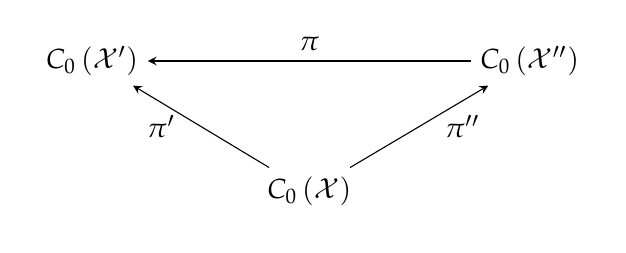
\begin{tikzpicture}
		\matrix (m) [matrix of math nodes,row sep=3em,column sep=4em,minimum width=2em]
		{
		C_0\left(\sX' \right)  & & C_0\left(\sX'' \right) \\ 
			& C_0\left(\sX \right)  & \\};
		\path[-stealth]
		(m-1-3) edge node [above] {$\pi$} (m-1-1)
		(m-2-2) edge node [left]  {$\pi'~~$} (m-1-1)
		(m-2-2) edge node [right] {$~~\pi''$} (m-1-3);
		\end{tikzpicture}
		\\ 	
	\end{itemize}
Following conditions hold:
\begin{enumerate}
	\item [(i)] 	If the category $\mathfrak{FinCov}$-$\sX$ is given by the Definition \ref{top_fin_cov_defn} then there is the natural equivalence of the categories $C_0:\mathfrak{FinCov}$-$\sX \cong \mathfrak{FinCov}$-$C_0\left(\sX \right)$.
	\item[(ii)] Any unordered pair of *-homomorphisms $\left( \pi',\pi''\right) $ from the above diagram is {compliant} (cf. Definition \ref{compliant_covering_defn}).
\end{enumerate}

\end{lem}
\begin{proof}
	(i) From the Theorem \ref{comm_fin_thm} it follows that there is a one-to-one correspondence between objects of $\mathfrak{FinCov}$-$\sX$ and objects of  $\mathfrak{FinCov}$-$C_0\left(\sX \right)$ given by
	$$
	\left(p:\widetilde{\sX} \to \sX \right) \mapsto 	C_0\left( p\right) :   C_0\left( \sX\right)    \hookto C_0\left( \widetilde{\sX}\right)
	$$
	where $C_0\left(p\right)$ is given by the Definition \ref{top_c_funct_defn}. If $p':\widetilde{\sX}' \to \sX$ and $p'':\widetilde{\sX}'' \to \sX$ are objects of $\mathfrak{FinCov}$-$\sX$ and $p: \widetilde{\sX}' \to \widetilde{\sX}''$ is a morphism of $\mathfrak{FinCov}$-$\sX$ then from the Lemma \ref{top_cov_cat_lem} it turns out that $p$ is a transitive finite-fold covering. From the equation \ref{top_c0_p_eqn} it follows that $p$ corresponds to the *-homomorphism
	\be\label{top_c_funct_lem_eqn}
	C_0\left(p \right):  C_0\left( \widetilde{\sX}''\right)    \to C_0\left( \widetilde{\sX}'\right).
	\ee
	So one has a functor from  $\mathfrak{FinCov}$-$\sX$ to  $\mathfrak{FinCov}$-$C_0\left( \sX\right)$. Let us define the inverse  functor. From the Theorem \ref{comm_fin_thm} it follows that any object $\pi: C_0\left( \sX\right) \hookto C_0\left( \widetilde{\sX}\right)$ of $\mathfrak{FinCov}$-$C_0\left( \sX\right) $ corresponds to a transitive finite-fold covering $p: \widetilde{\sX} \to \sX$ such that $\pi = C_0\left(p \right)$. If $C\left(p' \right): C_0\left( {\sX}\right)\to  C_0\left( \widetilde{\sX}'\right) $ and $C\left(p'' \right): C_0\left( {\sX}\right)\to C_0\left( \widetilde{\sX}''\right)$ are objects of $\mathfrak{FinCov}$-$C_0\left( \sX\right)$  and $\pi: C_0\left( \widetilde{\sX}''\right)    \to C_0\left( \widetilde{\sX}'\right)$ is a *-homomorphism such that $ C_0\left(p'\right) = \pi \circ C_0\left(p''\right)$ then $\pi$ corresponds to a continuous map $p: \widetilde{\sX}' \to \widetilde{\sX}''$ such than $p'= p \circ p''$. So one has the inverse functor from   $\mathfrak{FinCov}$-$C_0\left( \sX\right)$ to $\mathfrak{FinCov}$-$\sX$.\\
	(ii) If an open subset $\sU \subset \sX$ is connected, then $C_0\left(\sU\right)$ is not the ideal $\left.\mathscr C_0\left( \sX\right)\right|_{\sU_\a}$ is not a direct sum of no more than one nontrivial $C^*$-algebras.  The space $\sX$ is locally connected so any point has a fundamental system of connected neighborhoods. It turns out that
	$\mathscr C\stackrel{\mathrm{def}}{=} \left(\sX, \left\{\C_x\right\}_{x \in \sX}, C_0\left(\sX\right) \right)$ is locally trivial, so one can apply the Lemma \ref{comm_comply_lem}.	The conditions (a)-(d) of the Definition directly follow from (a)-(d) of the Lemma \ref{comm_comply_lem}.
	\end{proof}








\subsection{Induced representation}\label{comm_induced_finite_sec}
 \paragraph*{} 
Let us consider a compact  Spin-manifold, i.e. a Riemannian manifold $M$ with a  Spin-bundle $S$ (cf. \ref{comm_sp_tr_sec}). Denote by $\mu$  the Riemannian measure (cf.  \cite{do_carmo:rg}) on $M$. The bundle $S$ is Hermitian (cf. Definition \ref{top_herm_bundle_defn}) so there is a Hilbert space $L^2\left( M, S, \mu\right)$ (or  $L^2\left( M, S\right)$ in a simplified notation) (cf. \ref{top_herm_bundle_empt}) with the given by \eqref{top_bundle_herm_scalar_eqn} scalar product, i.e.
\be\label{comm_bundle_herm_scalar_eqn}
	\left( \xi, \eta\right)_{L^2\left(M, S\right)}\stackrel{\text{def}}{=} \int_{M}\left( \xi_x, \eta_x\right)_xd\mu
\ee
Moreover from 	\eqref{comm_bundle_repr_eqn} it follows that there is the natural representation
\be\label{comm_m_bundle_repr_eqn}
C_0\left(M\right) \to B\left( L^2\left(  M, S\right)\right). 
\ee
Let $p: \widetilde{M} \to M$ be a transitive covering.
Let us consider a family of open connected subsets $\left\{ \mathcal{U}_\a \subset M\right\}_{\a \in \mathscr A} $ such that
\begin{itemize}
	\item $\mathcal{U}_\a$ is evenly covered by $p$.
	\item The bundle $S$ is trivial on  $\mathcal{U}_\a$.
\end{itemize}
The space $M$ is compact, so there is a finite subfamily $\left\{ \mathcal{U}_\a \subset M\right\}_{\a \in \mathscr A}$ such that $M = \bigcup_{\a \in \mathscr A} \mathcal{U}_\a$.
From the Proposition \ref{smooth_part_unity_prop} it follows that there is a  finite family $\left\{ a_\a \in \Coo\left(  M\right) \right\}_{\a \in \mathscr A}$ such that
\begin{equation*}
\begin{split}
\supp ~a_\a \subset  \mathcal{U}_\a ,\\
1_{C\left( M\right) }= \sum_{\a \in \mathscr A}a_\a.
\end{split}
\end{equation*}
For any $\a \in \mathscr A$ denote by $e_\a = \sqrt{a_\a}\in C\left(  M\right)$.  From $a_\a \in \Coo\left(  M\right)$ it follows that
\be\label{top_e_smooth_eqn}
e_\a \in \Coo\left(  M\right).
\ee
If $\xi \in \Ga^\infty\left(M,S \right)$ is a smooth section then
\begin{equation*}
\begin{split}
\xi = \sum_{\a \in \mathscr A} \xi_\a, \text{ where } \xi_\a = a_\a \xi = e^2_\a \xi.
\end{split}
\end{equation*} 
For any $\a \in \mathscr A$ we can select an open connected subset $\widetilde{\mathcal{U}}_\a \subset \widetilde{M}$ such that $\widetilde{ \mathcal{U}}_\a$ is homeomorphically mapped onto $\mathcal{U}_\a$. 
Let $\widetilde{a}_\a = \mathfrak{lift}_{\widetilde{ \mathcal{U}}_\a} \left(a_\a \right) \in \Coo\left(\widetilde{M} \right)$, and let 
\be\label{top_te_eqn}
\widetilde{e}_\a = \mathfrak{lift}_{\widetilde{ \mathcal{U}}_\a} \left(e_\a \right)= \sqrt{\widetilde{a}_\a}\in \Coo\left(\widetilde{M} \right)
\ee (cf. Definition \ref{top_lift_desc_defn}).
If $\widetilde{\mathscr A} = G \times I$, $~\widetilde{e}_{\left(g, \a \right) }= g \widetilde{e}_\a$, for any $\left(g, \a \right) \in \widetilde{\mathscr A}$ then from the above construction it turns out
\be\label{comm_sum_1_eqn}
\begin{split}
1_{C\left(\widetilde{ M}\right) }= \sum_{g \in G}\sum_{\a \in \mathscr A}g\widetilde{e}^2_\a= \sum_{\widetilde{\a} \in \widetilde{\mathscr A}}\widetilde{e}_{\widetilde{\a}}^2~~,\\
\left( g\widetilde{e}_{\widetilde{\a}}\right)  \widetilde{e}_{\widetilde{\a}}= 0; \text{ for any nontrivial } g \in G.\\1_{C\left(\widetilde{ M}\right) } =\sum_{{\widetilde{\a} \in {\widetilde{\mathscr A}}}}\widetilde{e}_{\widetilde{\a}}\left\rangle \right\langle \widetilde{e}_{\widetilde{\a}},\\
\left\langle \widetilde{e}_{\widetilde{\a}'}, \widetilde{e}_{\widetilde{\a}''} \right\rangle 	\in C\left( M\right) 	
\end{split}
\ee
The set $\left\{\widetilde{e}_{\widetilde{\a}}\right\}_{\widetilde{\a}\in \widetilde{\mathscr A}}$ is $G$-invariant, i.e.
\be\label{comm_a_g_inv}
G\left\{\widetilde{e}_{\widetilde{\a}}\right\}_{\widetilde{\a}\in \widetilde{\mathscr A}}=\left\{\widetilde{e}_{\widetilde{\a}}\right\}_{\widetilde{\a}\in \widetilde{\mathscr A}}.
\ee
Similarly to the above construction any element in $\widetilde{\xi}\in \Ga\left(\widetilde{M},\widetilde{S} \right)$ can be represented as
\begin{equation}\label{cov_xi_repr}
\widetilde{\xi} = \sum_{g \in G} \sum_{\a \in \mathscr A} \left( g \widetilde{e}^2_\a\right)  \widetilde{\xi}.
\end{equation}
From $\left(g \widetilde{e}_\a \right)^2= g\widetilde{e}_\a e_\a$ and $$\supp ~\left( g\widetilde{e}_\a\right)  \widetilde{\xi}\subset \supp~g\widetilde{e}_\a \subset g \widetilde{\mathcal U}_\a$$   one can establish a $\C$-linear isomorphism
\begin{equation}\label{comm_smooth_iso_eqn}
\begin{split}
\varphi:\Ga\left(\widetilde{M},\widetilde{S} \right) \xrightarrow{\approx} C\left(\widetilde{M} \right)  \otimes_{C\left( M\right)}  \Ga\left(M,S \right), \\
\widetilde{\xi}=\sum_{g \in G} \sum_{\a \in \mathscr A} \left( g \widetilde{e}_\a\right)  \left( g \widetilde{e}_\a\right) \widetilde{\xi}  \mapsto \sum_{g \in G} \sum_{\a \in \mathscr A} g \widetilde{e}_\a \otimes \mathfrak{desc}\left(\left( g\widetilde{e}_\a\right)  \widetilde{\xi}\right) 
\end{split}
\end{equation}%\label{comm_fin_tens_eqn}
where $\mathfrak{desc}$ means $p$-descent (cf. Definition \ref{top_lift_desc_defn}). Note that there are dense with respect to Hilbert norm inclusions 
\bean
 \Ga\left( M, S\right) \subset L^2\left({M},{S}, \mu\right)= L^2\left({M},{S} \right),\\
C\left(\widetilde{M} \right) \otimes_{C\left(M \right) } L^2\left( M, S\right) \subset L^2\left(\widetilde{M},\widetilde{S}, \widetilde{\mu} \right)=L^2\left(\widetilde{M},\widetilde{S} \right)\\
\eean
where $\mu$ and $\widetilde{\mu}$ are Riemannian measure (cf.  \cite{do_carmo:rg}) on $M$, and $\widetilde{M}$ respectively.
If $\widetilde{a} \otimes \xi, \widetilde{b} \otimes \eta \in C\left(\widetilde{M} \right) \otimes_{C\left(M \right) } \Ga\left( M, S\right) \subset L^2\left(\widetilde{M},\widetilde{S} \right)$  then  the given by \ref{ind_act_form_eqn} scalar product $\left(\cdot, \cdot \right)_{\text{ind}}$ on  $ \Ga\left( M, S\right) \otimes L^2\left({M},{S}, \mu\right)$ satisfies to the following equation
\begin{equation}\label{comm_ind_l2_eqn}
\begin{split}
\left( \widetilde{a} \otimes \xi ,    \widetilde{b} \otimes \eta\right)_{\text{ind}}= \left(\xi, \left\langle \widetilde{a}, \widetilde{b}\right\rangle_{C\left(\widetilde{M} \right) } \eta \right)_{L^2\left({M},{S} \right)}=\\=\sum_{\widetilde{\a}\in \widetilde{\mathscr A}}\left(\xi, \left\langle \widetilde{a}_{\widetilde{\a}}\widetilde{a}, \widetilde{b}\right\rangle_{C\left(\widetilde{M} \right) } \eta \right)_{L^2\left({M},{S} \right)}
= \sum_{\widetilde{\a}\in \widetilde{\mathscr A}}\left(\xi, \mathfrak{desc}\left( \widetilde{a}_{\widetilde{\a}} \widetilde{a}^* \widetilde{b}\right)  \eta \right)_{L^2\left({M},{S} \right)}=\\=
\sum_{\widetilde{\a}\in \widetilde{\mathscr A}}~\int_M \left(\xi_x, \mathfrak{desc}\left( \widetilde{a}_{\widetilde{\a}} \widetilde{a}^* \widetilde{b}\right)  \eta_x \right)_x d\mu=
\\
=\sum_{\widetilde{\a}\in \widetilde{\mathscr A}}~ \int_{\widetilde{M}}\left( \lift_{\widetilde{\sU}_{\widetilde{\a}}}\left(\widetilde{e}_{\widetilde{\a}}\xi \right)_{\widetilde{x}},  \widetilde{a}^* \widetilde{b} ~\lift_{\widetilde{\sU}_{\widetilde{\a}}}\left(\widetilde{e}_{\widetilde{\a}}\eta \right)_{\widetilde{x}}\right)_{\widetilde{x}}d \widetilde{   \mu} =\\
= \int_{\widetilde{M}}\left( \lift_p\left(\xi \right)_{\widetilde{x}}, \widetilde{a}^* \widetilde{b} ~\lift_p\left(\eta \right)_{\widetilde{x}}\right)_{\widetilde{x}}d \widetilde{   \mu}
= \left( \widetilde{a}~ \lift_p\left(\xi \right),  \widetilde{b} ~\lift_p\left(\eta \right)\right)_{L^2\left(\widetilde{M},\widetilde{S} \right)}. \\
\end{split} 
\end{equation}
The equation \eqref{comm_ind_l2_eqn} means that $\left(\cdot, \cdot \right)_{\text{ind}}= \left(\cdot, \cdot \right)_{L^2\left(\widetilde{M},\widetilde{S} \right)}$, and taking into account the dense inclusion $C\left(\widetilde{M} \right) \otimes_{C\left(M \right) } \Ga\left( M, S\right) \subset L^2\left(\widetilde{M},\widetilde{S} \right)$ with respect to the Hilbert norm of $L^2\left(\widetilde{M},\widetilde{S}\right) $
one concludes that the space of induced representation coincides with $L^2\left(\widetilde{M},\widetilde{S}\right)$. 
 If $\varphi$ is the extension of the given by \eqref{comm_smooth_iso_eqn} map and  $\widetilde{a} \in C\left( \widetilde{M}\right)$ then following condition holds
\be\label{comm_fin_act_eqn}
\varphi\left( \widetilde{a}  \widetilde{\xi}\right) =\sum_{g \in G} \sum_{\a \in \mathscr A} \widetilde{a} \left( g  \widetilde{e}_\a\right)   \otimes \mathfrak{desc}\left(\left( g\widetilde{e}_\a\right)  \widetilde{\xi}\right) 
\ee
where the left part of \eqref{comm_fin_act_eqn} is relevant to the natural action of $C\left(\widetilde{M}\right)$ on $ L^2\left(\widetilde{M},\widetilde{S} \right)$,  the right part  is consistent with \eqref{ind_act_form_eqn}. It means that induced representation is given by the well known action $C\left(\widetilde{M}\right) \times L^2\left(\widetilde{M},\widetilde{S} \right) \to L^2\left(\widetilde{M},\widetilde{S} \right)$. So one has the following lemma.
\begin{lemma}\label{comm_ind_lem}
If the representation  $\widetilde{\rho}: C\left(\widetilde{M}\right) \to  B\left( \widetilde{   \H}\right)  $ is induced by the pair $$\left(C\left(M \right)\to B\left(  L^2\left(M,S \right)\right) ,\left(C\left(M \right) , C\left( \widetilde{M}\right) , G\left( \left.\widetilde{M}~\right|M\right) \right)  \right)$$ (cf. Definition \ref{induced_repr_defn}) then following conditions holds
\begin{enumerate}
	\item[(a)] There is the homomorphism of Hilbert spaces $\widetilde{   \H}\cong L^2\left(\widetilde{M},\widetilde{S} \right)$,
	\item[(b)] The representation $\widetilde{\rho}$ is given by the natural action of $C\left(\widetilde{M}\right)$ on $ L^2\left(\widetilde{M},\widetilde{S} \right)$.
\end{enumerate}
\end{lemma}
\begin{proof}
	(a) Follows from \eqref{comm_ind_l2_eqn},\\
	(b) Follows from \eqref{comm_fin_act_eqn}.
\end{proof}
For any $\widetilde{a} \in \Coo\left(\widetilde{M} \right)$ from \eqref{top_te_eqn} it follows that
$$
\widetilde{e}_{\widetilde{\a}'}\widetilde{a}\widetilde{e}_{\widetilde{\a}''}  \in \Coo\left(\widetilde{M} \right),
$$
hence one has
 $$
 \left\langle \widetilde{e}_{\widetilde{\a}'}~,~~\widetilde{a}\widetilde{e}_{\widetilde{\a}''}\right\rangle_{C\left(\widetilde{M} \right)}  = \mathfrak{desc}\left(\widetilde{e}_{\widetilde{\a}'}\widetilde{a}\widetilde{e}_{\widetilde{\a}''} \right) \in \Coo\left(M \right).
 $$
 Otherwise form $\widetilde{a} \notin \Coo\left(\widetilde{M} \right)$ it turns out that $\exists \widetilde{\a} \in \widetilde{\mathscr A}~~ \widetilde{e}^{~2}_{\widetilde{\a}} \widetilde{a} \notin \Coo\left(\widetilde{M} \right)$, hence
 $$
 \left\langle \widetilde{e}_{\widetilde{\a}}~,~~\widetilde{a}\widetilde{e}_{\widetilde{\a}}\right\rangle_{C\left(\widetilde{M} \right)}  =\Coo \mathfrak{desc}\left(\widetilde{e}^2_{\widetilde{\a}}\widetilde{a} \right) \notin \Coo\left({M} \right).
 $$
 Summarize above equations one concludes
 $$
\Coo\left(\widetilde{M} \right)= \left\{\left.\widetilde{a}\in C\left(\widetilde{M} \right)~\right|~  \left\langle \widetilde{e}_{\widetilde{\a}'}~,~~\widetilde{a}\widetilde{e}_{\widetilde{\a}''}\right\rangle_{C\left(\widetilde{M} \right)} \in \Coo\left( M\right); ~ \forall \widetilde{\a}', \widetilde{\a}'' \in \widetilde{\mathscr A} \right\}.
 $$
 From the Lemma \ref{smooth_matr_lem} it turns out that
 \begin{itemize}
 	\item The unital noncommutative finite-fold covering $\left(C\left({M} \right), C\left(\widetilde{M} \right), G\left( \widetilde{M}~|~M \right)\right) $ is {smoothly invariant} (cf. Definition \ref{smooth_defn}),
 \item 
 \be\label{comm_smooth_matr_eqn}
\Coo\left(\widetilde{M} \right) = C\left(\widetilde{M} \right)\bigcap 
 \mathbb{M}_{\left|\widetilde{\mathscr A}~ \right| }\left( \Coo\left( M\right) \right).
 \ee 	
 \end{itemize}
 
\subsection{Lift of the Dirac operator}\label{comm_d_sec}


For any $\widetilde{a} \in \Coo\left(\widetilde{M} \right)$ following condition holds
\bean
\widetilde{a} = \sum_{\widetilde{\a}\in \widetilde{\mathscr A}} \widetilde{\ga}_{\widetilde{\a}}= \sum_{\widetilde{\a}\in \widetilde{\mathscr A}} \widetilde{\phi}_{\widetilde{\a}}\widetilde{\psi}_{\widetilde{\a}}; \text{ where } \widetilde{\phi}_{\widetilde{\a}}= \widetilde{e}_{\widetilde{\a}},~ \widetilde{\psi}_{\widetilde{\a}}= \widetilde{a}\widetilde{e}_{\widetilde{\a}},~ \widetilde{\ga}_{\widetilde{\a}}=\widetilde{a}_{\widetilde{\a}}\widetilde{e}^2_{\widetilde{\a}}.
\eean
Denote by $\Om^1_{\slashed D}$  the {module of differential forms associated} with the spectral triple  $$\left(\Coo\left({M} \right), L^2\left(M,S \right), \slashed D\right)$$ (cf. Definition \ref{ass_cycle_defn}). Denote by ${\phi}_{\widetilde{\a}} = \mathfrak{desc} \left(\widetilde{\phi}_{\widetilde{\a}} \right)$, ${\psi}_{\widetilde{\a}} = \mathfrak{desc} \left(\widetilde{\psi}_{\widetilde{\a}} \right)$,  ${\ga}_{\widetilde{\a}} = \mathfrak{desc} \left(\widetilde{\ga}_{\widetilde{\a}} \right)\in \Coo\left({M} \right)$. Let us define a $\C$-linear map
\bean
\nabla: \Coo\left(\widetilde{M} \right) \to \Coo\left(\widetilde{M} \right) \otimes_{\Coo\left({M} \right)}\Om^1_{\slashed D},\\
\widetilde{a} \mapsto \sum_{\widetilde{\a}\in \widetilde{\mathscr A}}\left(  \widetilde{\phi}_{\widetilde{\a}} \otimes \left[\slashed D, {\psi}_{\widetilde{\a}}  \right] +\widetilde{\psi}_{\widetilde{\a}} \otimes \left[\slashed D, {\phi}_{\widetilde{\a}}   \right] \right).
\eean
For any $a \in \Coo\left({M} \right)$ following condition holds
 \bean
 \nabla\left(\widetilde{a}a \right)=  \sum_{\widetilde{\a}\in \widetilde{\mathscr A}}\left(  \widetilde{\phi}_{\widetilde{\a}} \otimes \left[\slashed D, {\psi}_{\widetilde{\a}} a  \right] +\widetilde{\psi}_{\widetilde{\a}}a \otimes \left[\slashed D, {\phi}_{\widetilde{\a}}   \right] \right) =\\= \sum_{\widetilde{\a}\in \widetilde{\mathscr A}} \widetilde{\phi}_{\widetilde{\a}} \otimes \left[\slashed D, {\psi}_{\widetilde{\a}}  \right]a+\widetilde{\phi}_{\widetilde{\a}} \otimes \widetilde{\psi}_{\widetilde{\a}}\left[\slashed D,  a  \right] +\widetilde{\psi}_{\widetilde{\a}} \otimes \left[\slashed D, {\phi}_{\widetilde{\a}}   \right]a=\\= \sum_{\widetilde{\a}\in \widetilde{\mathscr A}}\left(  \widetilde{\phi}_{\widetilde{\a}} \otimes \left[\slashed D, {\psi}_{\widetilde{\a}}   \right] +\widetilde{\psi}_{\widetilde{\a}} \otimes \left[\slashed D, {\phi}_{\widetilde{\a}}  \right] \right) a+
 \sum_{\widetilde{\a}\in \widetilde{\mathscr A}}\widetilde{\phi}_{\widetilde{\a}}\widetilde{\psi}_{\widetilde{\a}}\left[ \slashed D,a\right]=
 \nabla\left( \widetilde{a}\right) a + \widetilde{a}\otimes  \left[ \slashed D,a\right]. 
 \eean
The comparison of the above equation and \eqref{conn_triple_eqn} states that $\nabla$ is a connection. If $g \in  G\left( \left.\widetilde{M}~\right|M\right)$ then from $\mathfrak{desc}\left(g\widetilde{\phi}_{\widetilde{\a}}\right) = {\phi}_{\widetilde{\a}} $ and $\mathfrak{desc}\left(g\widetilde{\psi}_{\widetilde{\a}}\right) = {\psi}_{\widetilde{\a}} $ it follows that
\bean
\nabla\left(g\widetilde{a} \right)=  \nabla\left(\sum_{\widetilde{\a}\in \widetilde{\mathscr A}} \left( g\widetilde{\phi}_{\widetilde{\a}}\right) \left( g\widetilde{\psi}_{\widetilde{\a}}\right)\right)=\\=\sum_{\widetilde{\a}\in \widetilde{\mathscr A}}\left( g \widetilde{\phi}_{\widetilde{\a}} \otimes \left[\slashed D, {\psi}_{\widetilde{\a}}   \right] +g\widetilde{\psi}_{\widetilde{\a}} \otimes \left[\slashed D, {\phi}_{\widetilde{\a}}   \right] \right)= g \left( \nabla\left(\widetilde{a} \right)\right),  
\eean
i.e. $\nabla$ is  $G$-{equivariant} (cf. \eqref{equiv_conn_eqn}). 
If $\xi \in \Dom~\slashed D$ then following conditions hold
\bean
\supp~\widetilde{\phi}_{\widetilde{\a}} \otimes \left[\slashed D, {\psi}_{\widetilde{\a}}   \right]\xi \in \widetilde{\mathcal{U}}_{\widetilde\a},\\
\supp~\widetilde{\psi}_{\widetilde{\a}} \otimes \left[\slashed D, {\phi}_{\widetilde{\a}}   \right]\xi \in \widetilde{\mathcal{U}}_{\widetilde\a},
\eean
hence one has
\bean
\widetilde{\phi}_{\widetilde{\a}} \otimes \left[\slashed D, {\psi}_{\widetilde{\a}}   \right]\xi = \mathfrak{lift}_{\widetilde{\mathcal{U}}_{\widetilde\a}} \left({\phi}_{\widetilde{\a}}  \left[\slashed D, {\psi}_{\widetilde{\a}}   \right]\xi \right),\\
\widetilde{\psi}_{\widetilde{\a}} \otimes \left[\slashed D, {\phi}_{\widetilde{\a}}   \right]\xi = \mathfrak{lift}_{\widetilde{\mathcal{U}}_{\widetilde\a}} \left({\psi}_{\widetilde{\a}}  \left[\slashed D, {\phi}_{\widetilde{\a}}   \right]\xi \right).
\eean
From \eqref{comm_matr_x_eqn} it turns out $\widetilde{\psi}_{\widetilde{\a}}  \left[\slashed D, {\phi}_{\widetilde{\a}}   \right] =   \left[\slashed D, {\phi}_{\widetilde{\a}}   \right]\widetilde{\psi}_{\widetilde{\a}}$, hence
\bean
\widetilde{\phi}_{\widetilde{\a}} \otimes \left[\slashed D, {\psi}_{\widetilde{\a}}   \right]\xi + \widetilde{\psi}_{\widetilde{\a}} \otimes \left[\slashed D, {\phi}_{\widetilde{\a}}   \right]\xi =\\= \mathfrak{lift}_{\widetilde{\mathcal{U}}_{\widetilde\a}}\left(\left( \left[\slashed D, {\phi}_{\widetilde{\a}}   \right]{\psi}_{\widetilde{\a}}+{\phi}_{\widetilde{\a}}  \left[\slashed D, {\psi}_{\widetilde{\a}}   \right] \right)\xi \right)= \mathfrak{lift}_{\widetilde{\mathcal{U}}_{\widetilde\a}}\left(\left[\slashed D, {\ga}_{\widetilde{\a}}   \right] \xi\right). 
\eean
If $\widetilde{\slashed D}$ is $\left(C\left(M\right) , C\left(\widetilde{M} \right) , G\left(\widetilde{M}~|M \right)   \right)$-lift of $\slashed D$ (cf. Definition \ref{triple_conn_lift_defn}), $\xi \in \H^\infty= \Ga^\infty\left(M, \sS \right)$ and 
$$
p^{-1}{\slashed D} \in \mathscr Hom \left(\mathscr C^\infty \left(M, \left\{\sS_x\right\}_{x \in M}, \Ga\left(M, \sS \right) \right), \mathscr C^\infty \left(M, \left\{\sS_x\right\}_{x \in M}, \Ga\left(M, \sS \right) \right) \right)
$$
is the $p$-{inverse image} of $\slashed D$ (cf. Definition \ref{top_smooth_inv_im_defn} and Example \ref{top_smooth_inv_im_defn})
then 
from \eqref{d_defn_eqn},  $\mathfrak{lift}_{\widetilde{\mathcal{U}}_{\widetilde\a}}\left( {\ga}_{\widetilde{\a}}\right) = \widetilde{\ga}_{\widetilde{\a}}$ and $\sum_{\widetilde{\a}\in \widetilde{\mathscr A}}~ \widetilde{\ga}_{\widetilde{\a}} = \widetilde{a}$ and taking into account \eqref{comm_lift_comp_eqn}  one has
\be\nonumber
\begin{split}
\widetilde{\slashed D}\left(\widetilde{a} \otimes \xi \right)= \sum_{\widetilde{\a}\in \widetilde{\mathscr A}}\left(  \widetilde{\phi}_{\widetilde{\a}} \otimes \left[\slashed D, {\psi}_{\widetilde{\a}}  \right]\xi +\widetilde{\psi}_{\widetilde{\a}} \otimes \left[\slashed D, {\phi}_{\widetilde{\a}}   \right] \xi\right)+ \widetilde{a} \otimes \slashed D\xi =\\=\sum_{\widetilde{\a}\in \widetilde{\mathscr A}}    
\mathfrak{lift}_{\widetilde{\mathcal U}_{\widetilde{   \a}}}\left( \left[{\slashed D}, {\ga}_{\widetilde{\a}}  \right]\right) \left(1 \otimes \xi\right)  +\widetilde{a} \otimes \slashed D\xi =\\  = \left[p^{-1}{\slashed D} , {\widetilde{a}}   \right]\left(1 \otimes \xi \right)+ \widetilde{a} \otimes \slashed D\xi =\\=
\left[  p^{-1}{\slashed D} , {\widetilde{a}}   \right]\left(1 \otimes \xi \right)+ \widetilde{a}~\left(  p^{-1}{\slashed D}\right) \left( 1  \otimes \xi\right) = \left(  p^{-1}{\slashed D}\right) \left(\widetilde{a} \otimes \xi \right),
\end{split}
\ee
it follows that
\be\label{comm_d_eqn}
\widetilde{\slashed D} =  p^{-1}{\slashed D}.
\ee

\subsection{Coverings of spectral triples}
\paragraph*{}
From \eqref{comm_sum_1_eqn} it turns that 
 $C\left(M \right)$-module $C\left(\widetilde{M} \right)$ is generated by  a finite set $\left\{\widetilde{e}_{\widetilde{\a}}\right\}_{\widetilde{\a}\in \widetilde{\mathscr A}}$, i.e.
$$
C\left(\widetilde{M} \right) = \sum_{\widetilde{\a}\in \widetilde{\mathscr A}}  \widetilde{e}_{\widetilde{\a}}~C(M).
$$ 
Also from \eqref{comm_sum_1_eqn} it turns out $\left\langle \widetilde{e}_{\widetilde{\a'}}, \widetilde{e}_{\widetilde{\a''}}\right\rangle_{C\left(\widetilde{M} \right) } \in \Coo\left(M \right)$, i.e.  the set $\left\{\widetilde{e}_{\widetilde{\a}}\right\}_{\widetilde{\a}\in \widetilde{\mathscr A}}$ , satisfies to the condition (a) of the Lemma \ref{smooth_matr_lem}. From \eqref{comm_a_g_inv} it turns out that 
$\left\{\widetilde{e}_{\widetilde{\a}}\right\}_{\widetilde{\a}\in \widetilde{\mathscr A}}$ is $G$-invariant, i.e.
\be\nonumber
G\left\{\widetilde{e}_{\widetilde{\a}}\right\}_{\widetilde{\a}\in \widetilde{\mathscr A}}=\left\{\widetilde{e}_{\widetilde{\a}}\right\}_{\widetilde{\a}\in \widetilde{\mathscr A}}~,
\ee
 hence the set $\left\{\widetilde{e}_{\widetilde{\a}}\right\}_{\widetilde{\a}\in \widetilde{\mathscr A}}$ , satisfies to the condition (b) of the Lemma \ref{smooth_matr_lem}. From the Lemma \ref{smooth_matr_lem} it turns out that  the unital noncommutative finite-fold covering $\left(C\left(M \right) , C\left( \widetilde{M}\right) , G \right)$ is {smoothly invariant}. Taking into account the Section \ref{comm_d_sec}  one has the following theorem. 

\begin{thm}\label{comm_fin_sp_tr_thm} If $\widetilde{\slashed D}=\lift_p\left( \slashed D\right)$ then the spectral triple $\left(C^{\infty}\left( \widetilde{M}\right) , L^2\left( \widetilde{M}, \widetilde{S}\right) , p^{-1}{\slashed D}\right)$ is the $\left(C\left(M \right) , C\left( \widetilde{M}\right) , G\left( \left.\widetilde{M}~\right|M\right)  \right)$-lift of $\left(C^{\infty}\left( M\right) , L^2\left( M, S\right) ,\slashed D\right)$.
\end{thm}

\subsection{Unoriented spectral triples}\label{comm_sp_tr} 
\paragraph*{}
Let $M$ be an unoriented  Riemannian manifold, and let $\widetilde{M} \to M$ be a two listed covering by oriented  Riemannian manifold $\widetilde{M}$ with Spin-structure given by Spin-bundle $\SS$. From the construction of the Section \ref{unoti_defn_sec} it follows that there is a commutative unoriented spectral triple 
\be\label{comm_equ}
\left(\Coo\left(M \right), L^2\left(\widetilde{M}, \widetilde{\SS}\right)^{\Z_2}=L^2\left({M}, {\SS}\right), \slashed D  \right).
\ee


\paragraph*{} This section contains an algebraic version of the Proposition \ref{comm_cov_mani} in case of infinite coverings.
\section{Infinite coverings}

\subsection{Inverse limits of coverings in topology}\label{top_inf_to_sec}
%\paragraph*{}

\begin{definition}\label{top_sec_defn}
		Let $\La$ be a directed set (cf. Definition \ref{directed_set_defn}) such that there is the unique minimal element $\la_{\mathrm{min}} \in \La$.
	Let $\mathcal X$ be a connected locally connected second-countable topological space. Consider a full subcategory $\mathfrak{S}$ the {finite covering category} of $\sX$ (cf. Definition \ref{top_fin_cov_defn}). The set of objects is marked by $\La$, i.e. the set of objects is a family $\left\{p_\la: \sX_\la\to \sX\right\}_{\la \in \La}$ of transitive finite-fold coverings such that $\sX_{\la_{\mathrm{min}}}= \sX$, and $p_{\la_{\mathrm{min}}}= \Id_\sX$. Morphism from $p_\mu : \sX_\mu \to \sX$ to $p_\nu : \sX_\nu \to \sX$ is a continuous map $p: \sX_\mu \to \sX_\nu$ such that $p_\mu = p_\nu \circ p$. We require that
	\be\label{top_ord_eqn}
	\begin{split}
		\mu \ge \nu  \text{ if and only if there is a coninuous map } p: \sX_\mu \to \sX_\nu \\
		\text{ such that } p_\mu = p_\nu \circ p .
	\end{split}
	\ee
	We say that $\mathfrak{S}$ is a \textit{topological finite covering category} and we write $\mathfrak{S}\in \mathfrak{FinTop}$.
\end{definition}


\begin{definition}\label{top_sec_p_defn}
	Let $\mathfrak{S}_\sX$ be a topological finite covering category with the set of objects $\left\{p_\la: \sX_\la\to \sX\right\}_{\la \in \La}$. Suppose that there are base points $x_0 \in \sX$ and $x^\la_0 \in \sX_\la$ such that for any $\la \in \La$ the $p_\la$ is a pointed map $\left( \sX_\la, x^\la_0\right) \to \left( \sX, x_0\right)$ (cf. Definition \ref{top_pointed_defn}). Let us consider a subcategory $\mathfrak{S}_{\left( \sX, x_0\right) }= \left\{\left( \sX_\la, x^\la_0\right) \to \left( \sX, x_0\right)\right)\}$  of $\mathfrak{S}_\sX$  such that any morphism  $p^\mu_\nu: \left( \sX_\mu, x^\mu_0\right) \to \left( \sX_\nu, x^\nu_0\right)$ of $\mathfrak{S}_{\left( \sX, x_0\right) }$ is a pointed  map.  We say that $\mathfrak{S}_{\left( \sX, x_0\right) }$ is a \textit{pointed topological finite covering category} and we write $$\mathfrak{S}_{\left( \sX, x_0\right) }\in \mathfrak{FinTop}^{\text{pt}}.$$
\end{definition}
\begin{remark}
	The category $\mathfrak{S}_{\left( \sX, x_0\right) }$ is a  subcategory of the category $\mathfrak{FinCov}$-$\left( \sX, x_0\right) $ the {pointed finite covering category} of $\left( \sX, x_0\right)$
\end{remark}
\begin{remark}
	The category $\mathfrak{S}^{\mathrm{pt}}$ is equivalent to the pre-order category $\La$ (cf. Definition \ref{preordercat_defn}).
\end{remark}


\begin{definition}\label{top_cov_trans_defn} Let  $\mathfrak{S}_{\left( \sX, x_0\right) }= \left\{\left( \sX_\la, x^\la_0\right) \to \left( \sX, x_0\right)\right\}_{\la \in \La} \in \mathfrak{FinTop}^{\mathrm{pt}}$ be a pointed topological finite covering category, and let
	$\widehat{\mathcal{X}} = \varprojlim \mathcal{X}_\la$ be the inverse limit  in the category of topological spaces and continuous maps (cf. \cite{spanier:at}). If $\widehat{p}: \widehat{\mathcal{X}} \to \mathcal{X}$ is the natural continuous map then a homeomorphism $g$ of the space $\widehat{\mathcal{X}}$ is said to be a \textit{covering  transformation} if a following condition holds
	$$
	\widehat{p} = \widehat{p} \circ g.
	$$
	The group $\widehat{G}$ of such homeomorphisms is said to be the \textit{group of  covering  transformations} of $\mathfrak S$. Denote by $G\left(\left.\widehat{\sX}~\right|\sX \right)\stackrel{\text{def}}{=}\widehat{G}$. 
\end{definition}
\begin{lemma}\label{top_surj_group_lem}
	Let  $\mathfrak{S}_{\left( \sX, x_0\right) }= \left\{\left( \sX_\la, x^\la_0\right) \to \left( \sX, x_0\right)\right\}_{\la \in \La} \in \mathfrak{FinTop}^{\mathrm{pt}}$ be a pointed topological finite covering category, and let
	$\left( \widehat{\mathcal{X}}, \widehat{x}_0 \right) = \varprojlim \left( \sX_\la, x^\la_0\right)$ be the inverse limit  in the category of topological spaces and continuous maps. There is the natural group isomorphism $G\left(\left.\widehat{\sX}~\right|\sX \right) \cong \varprojlim G\left({\mathcal{X}}_\la~|~\mathcal X \right)$. For any $\la \in \La$ there is the natural surjective homomorphism $h_\la:G\left(\left.\widehat{\sX}~\right|\sX \right) \to G\left(\left.{\sX}_\la~\right|\sX \right)$ and $\bigcap_{\la \in \La} \ker h_\la$ is a trivial group.
\end{lemma}
\begin{proof}
	There is a continuous map $\widehat{p}:\left( \widehat{\mathcal{X}}, \widehat{x}_0 \right)\to \left( {\mathcal{X}}, {x}_0 \right)$ and 	for any $\la \in \La$ there is the natural continuous map $\widehat{p}_\la:\widehat{p}:\left( \widehat{\mathcal{X}}, \widehat{x}_0 \right)\to \left( {\mathcal{X}}_\la, {x}^\la_0 \right)$
	Let $\widehat{x}' \in \widehat{\mathcal{X}}$ be such that $\widehat{p}\left( \widehat{x}'\right)=x_0$.  If  $x'_\la = \widehat{p}_\la\left(\widehat{x}' \right)$ and $x_\la = \widehat{p}_\la\left(\widehat{x}_0 \right)$ then $p_\la\left(x_\la \right)=p_\la\left(x'_\la \right)$, where $p_\la : \left( {\mathcal{X}}_\la, {x}^\la_0 \right)\to \left( {\mathcal{X}}, {x}_0 \right)$ is the natural covering. Since $p_\la$ is transitive for any $\la \in \La$ there is the unique $g_\la \in G\left( \mathcal{X}_\la~|~\mathcal{X}\right)$ such that $x'_\la = g_\la x_\la$. In result there is a sequence $\left\{g_\la \in G\left( \mathcal{X}_\la~|~\mathcal{X}\right)\right\}_{\la \in \La}$ which satisfies to the following condition
	\begin{equation*}
	g_\mu \circ	p^\la_\mu = p^\la_\mu \circ g_\la
	\end{equation*}
	where $\la > \mu$ and $p^\la_\mu : \mathcal X_\la \to \mathcal X_\mu$ is a morphism of $\mathfrak{S}_{\left( \sX, x_0\right) }$. The sequence $\left\{g_\la \right\}$ naturally defines an element $\widehat{g} \in \varprojlim G\left(\mathcal X_\la~|\mathcal X \right)$. 
	Let us define an homeomorphism $\varphi_{\widehat{g}}: \widehat{\mathcal{X}} \to \widehat{\mathcal{X}}$ by a following construction. 	If $\widehat{x}''\in \widehat{\mathcal{X}}$ is any point  then there is the family $\left\{x''_\la \in \mathcal X_\la\right\}_{\la \in \La}$ such that
	$$
	x''_\la = \widehat{p}_\la\left(\widehat{x}''\right) .
	$$
	On the other hand there is the family $\left\{x''^{\widehat{g}}_\la \in \mathcal X_\la\right\}_{\la \in \La}$
	$$
	x''^{\widehat{g}}_\la=g_\la x''_\la
	$$
	which for any $n > m$ satisfies to the following condition
	\begin{equation*}\label{top_xg_eqn}
	p^\la_\mu\left(x''^{\widehat{g}}_\la \right) = {x}''^{g}_\mu.
	\end{equation*}
	From the above equation and properties of inverse limits it follows that there is the unique $\widehat{x}''^{\widehat{g}} \in \widehat{\mathcal{X}}$ such that 
	$$
	\widehat{p}_\la \left( \widehat{x}''^{\widehat{g}}\right) = x''^{\widehat{g}}_\la; ~~ \forall \la \in \La.
	$$
	The required homeomorphism $\varphi_{\widehat{g}}$ is given by
	$$
	\varphi_{\widehat{g}}\left( \widehat{x}''\right)  = \widehat{x}''^{\widehat{g}}.
	$$
	From $\widehat{p}\circ \varphi_{\widehat{g}} = \widehat{p}$ it follows that $\varphi_{\widehat{g}}$ corresponds to an element in $G\left(\widehat{  \mathcal X}~|~\mathcal X \right)$ which mapped onto $g_\la$ for any $\la \in \La$. Otherwise $\varphi_{\widehat{g}}$ naturally corresponds to the element $\widehat{g} \in \varprojlim G\left(\mathcal X_\la~|\mathcal X \right)$, so one has  the natural group isomorphism $G\left(\left.\widehat{\sX}~\right|\sX \right) \cong \varprojlim G\left({\mathcal{X}}_\la~|~\mathcal X \right)$.
	From the above construction it turns out that any homeomorphism $\widehat{g} \in G\left(\widehat{  \mathcal X}~|~\mathcal X \right)$ uniquely depends on $\widehat{x}'=\widehat{g}\widehat{x}_0\in \widehat{p}^{-1} \left( x_0\right)$.  It follows that there is the 1-1 map $\varphi:\widehat{p}^{-1}\left(x_0 \right)\xrightarrow{\approx} G\left(\left.\widehat{\sX}~\right|\sX \right)$. Since the covering $p_\la : \mathcal{X}_\la\to\mathcal X$ is regular there is the 1-1 map	$\varphi_\la:p_\la^{-1}\left(x_0 \right)\xrightarrow{\approx} G\left(\left.{\sX}_\la~\right|\sX \right)$. The natural surjective map
	$$
	\widehat{p}^{-1}\left(x_0 \right) \to  p_\la^{-1}\left(x_0 \right)
	$$
	induces the surjective homomorphism $G\left(\left.\widehat{\sX}~\right|\sX \right) \to G\left(\left.{\sX}_\la~\right|\sX \right)$. If $\widehat{g} \in \bigcap_{\La \in \la} \ker h_\la$ is not trivial then $\widehat{g} \widehat{x}_0 \neq  \widehat{x}_0$ and there is $n \in \mathbb{N}$ such that $\widehat{p}_\la\left(\widehat{x}_0\right)\neq \widehat{p}_\la\left(\widehat{g}\widehat{x}_0\right)= h_\la\left(\widehat{g} \right) \widehat{p}_\la\left(\widehat{x}_0\right)$, so $h_\la\left(\widehat{g} \right)  \in G\left(\left.{\sX}_\la~\right|\sX \right)$ is not trivial and $\widehat{g} \notin \ker h_\la$. From this contradiction it follows that $\bigcap_{\la \in \La} \ker h_\la$ is a trivial group.
\end{proof}
\begin{definition}\label{top_?oh_defn}
	Let $\mathfrak{S}^{\mathrm{pt}}  = \left\{p_{\la}:\left( \mathcal{X}_\la, x^\la_0 \right) \to \left( \mathcal{X}, x_0 \right)\right\}_{\la \in \La} \in \mathfrak{FinTop}^{\mathrm{pt}}$ be a pointed topological finite covering category. The pair $\left(\left( \mathcal{Y}, y_0\right) ,\left\{p^{\mathcal Y}_\la\right\}_{\la \in \La} \right) $ of a (discrete) pointed set $\left( \mathcal{Y}, y_0\right)$ with and  
	preserving base-point surjective  maps $p^{\mathcal Y}_\la:\left( \sY,y_0\right) \to \left( \sX_\la, x^\la_0\right)$ is said to be a \textit{coherent system} if for any $\mu,\nu \in \La$ such that $\mu > \nu$ a following diagram  
	\newline
	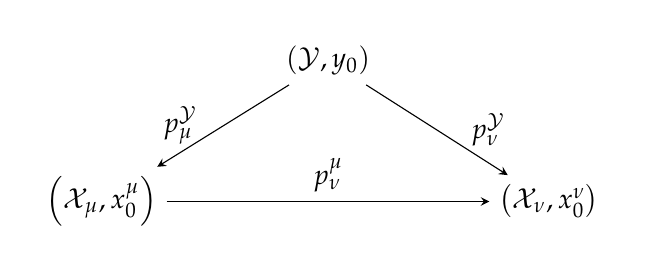
\begin{tikzpicture}
	\matrix (m) [matrix of math nodes,row sep=3em,column sep=4em,minimum width=2em]
	{
		&  \left( \mathcal{Y}, y_0\right) &  \\
		\left( \sX_\mu, x^\mu_0\right) &  & \left( \sX_\nu, x^\nu_0\right) \\};
	\path[-stealth]
	(m-1-2) edge node [left] {$p^{\mathcal Y}_\mu~~$} (m-2-1)
	(m-1-2) edge node [right] {$~~~p^{\mathcal Y}_{\nu}$} (m-2-3)
	(m-2-1) edge node [above] {$p^\mu_\nu$}  (m-2-3);
	
	\end{tikzpicture}
	\newline
	is commutative.	
\end{definition}

\begin{definition}\label{comm_top_constr_defn}
	Let $\mathfrak{S}_{\left( \sX, x_0\right)}= \left\{\left( \sX_\la, x^\la_0\right) \to \left( \sX, x_0\right)\right\}_{\la \in \La}\in \mathfrak{FinTop}^{\text{pt}}$ be a pointed topological finite covering category. A coherent system $\left(\left(\mathcal{Y}, y_0\right),\left\{p^{\mathcal Y}_\la\right\} \right)$ is said to
	be a \textit{connected covering} of $\left(\mathfrak{S}, x_0\right)$ if $\mathcal Y$ is a connected topological space and $p^{\mathcal Y}_\la$ is a transitive covering  for any $\la\in \La$.  We will use following notation $\left(\left(\mathcal{Y}, y_0\right),\left\{p^{\mathcal Y}_\la\right\} \right)\downarrow \mathfrak{S}_{\left( \sX, x_0\right)}$ or simply $\left(\mathcal{Y}, y_0\right) \downarrow  \mathfrak{S}_{\left( \sX, x_0\right)}$.
\end{definition}

\begin{definition}\label{top_spec_defn}
	Let $\left(\left(\mathcal{Y}, y_0\right),\left\{p^{\mathcal Y}_\la\right\} \right)$ be  a coherent system   of $\left(\mathfrak{S}, x_0\right)$ and $y \in \mathcal{Y}$. A subset  $\mathcal V \subset \mathcal{Y}$ is said to be \textit{special} if  for any  $\la \in \La$  the restriction $p^{\mathcal Y}_\la|_{\mathcal V}:\mathcal{V}\to \sX_\la$ is a bijection onto the open connected subset  $p^{\mathcal Y}_\la\left( {\mathcal V}\right)\subset \sX_\la$.
\end{definition}
\begin{empt}  Consider the situation of the Definition \ref{comm_top_constr_defn}
	Let $y \in \mathcal Y$ and let $x_\la = p^{\mathcal Y}_\la\left( y\right)$ and  $x =  p^{\mathcal Y}\left( y\right)\in   \mathcal X$. 
	The space $\mathcal X$ is locally connected, it turns out  there is an open connected neighborhood  $\mathcal U$ of $x$ such that for any $\la \in \La$ there is a connected open $\mathcal U_\la$ of $x_\la$ such that $p_{\la}|_{\mathcal U_\la}: \mathcal U_\la\xrightarrow{\approx}\mathcal U$ is a homeomorphism.
\end{empt}
%\begin{remark}
%	For any $\la \in \La$ the space $\mathcal X_\la$ is locally connected, so from the  Theorem \ref{comm_sep_thm} for any point $x \in \mathcal X_\la$ there is an open connected neighborhood $\mathcal U \subset \mathcal X_\la$.
%\end{remark}
\begin{remark}
	If $\left(\left(\mathcal{Y}, y_0\right),\left\{p^{\mathcal Y}_\la\right\} \right)$ is  a covering  of $\left(\mathfrak{S}, x_0\right)$ then the set of special sets is a base of the topology of $\mathcal{Y}$.
\end{remark}

\begin{lemma}\label{top_equ_borel_set_lem}
	Let $\widehat{\mathcal{X}} = \varprojlim_{\la \in \La} \mathcal{X}_\la$ be the inverse limit  in the category of topological spaces and continuous maps. Any special set of $\widehat{\mathcal{X}}$ is a Borel subset of $\widehat{\mathcal{X}}$.
	
\end{lemma}\label{top_spec_borel_lem}
\begin{proof}
	If $\mathcal U_\la\subset \mathcal X_\la$ is an open set then $\widehat{p}_\la^{-1} \left(\mathcal U_\la \right) \subset \widehat{\mathcal X}$ is open. 
	If $\widehat{\mathcal U}$ is a special set then $\widehat{\mathcal U} = \bigcap_{\la\in\La} \widehat{p}_\la^{-1} \circ \widehat{p}_\la\left(\widehat{\mathcal U}\right)$, i.e. $\widehat{\mathcal U}$ is a countable intersection of open sets. So $\widehat{\mathcal U}$ is a Borel subset.	
\end{proof}
\begin{definition}\label{comm_top_constr_morph_defn}
	Let us consider the situation of the Definition \ref{comm_top_constr_defn}. A \textit{morphism} from $\left(\mathcal{Y}',\left\{p^{\mathcal Y'}_\la\right\}\right)\downarrow\mathfrak{S}_{\left( \sX, x_0\right)}$ to $\left(\mathcal{Y}'',\left\{p^{\mathcal Y''}_\la\right\}\right)\downarrow\mathfrak{S}_{\left( \sX, x_0\right)}$ is a preserving base-point covering   $f: \left(\mathcal{Y}', y'_0\right) \to \left(\mathcal{Y}'', y''_0\right)$ such that
	$$
	p_\la^{\mathcal Y''} \circ f= p_\la^{\mathcal Y'} 
	$$
	for any $\la \in \La$.
	
\end{definition}
\begin{empt}\label{comm_top_constr}
	There is a category with objects and morphisms described by Definitions \ref{comm_top_constr_defn}, \ref{comm_top_constr_morph_defn}. Denote by $\downarrow \mathfrak{S}_{\left( \sX, x_0\right)}$ this category.
\end{empt}
\begin{lemma}\label{top_universal_covering_lem}
If $\mathfrak{S}_{\left( \sX, x_0\right)}= \left\{\left( \sX_\la, x^\la_0\right) \to \left( \sX, x_0\right)\right\}_{\la \in \La} \in \mathfrak{FinTop}^{\mathrm{pt}}$  then there is the final object of the category $\downarrow \mathfrak{S}_{\left( \sX, x_0\right)}$  described in \ref{comm_top_constr}.
\end{lemma}


\begin{proof}
	Let $\widehat{\mathcal{X}} = \varprojlim_{\la \in \La} \mathcal{X}_\la$ be the inverse limit  in the category of topological spaces and continuous maps and $\widehat{p}_\la: \widehat{\mathcal{X}}\to \sX_\la$, $\widehat{p}: \widehat{\mathcal{X}}\to \sX$ be natural continuous maps. Denote by $\overline{\mathcal X}$ a topological space such that
	\begin{itemize}
		\item $\overline{\mathcal X}$ coincides with $\widehat{\mathcal X}$ as a set. 
		\item A set of special sets of $\widehat{\mathcal X}$ is a base of the topology of $\overline{\mathcal X}$.
	\end{itemize}
	The family of base-points $\left\{x^0_\la\in \sX_\la\right\}$ naturally defines the unique point $\widehat{x}_0 \in \widehat{  \mathcal X}$. There is the bijective map $\widehat{  \mathcal X}\cong \overline{   \mathcal X}$, so there is the unique $\widetilde{x}_0\in \overline{   \mathcal X}$ which is the image of $\widehat{x}_0$. Denote by $\widetilde{\sX}\subset \overline{   \mathcal X}$ the connected component of $\widetilde{x}_0$. The natural continuous maps $\widehat{p} : \widehat{  \mathcal X} \to \sX$ and  $\widehat{p}_\la : \widehat{  \mathcal X} \to \sX_\la$ for all $\la \in \La$ yield preserving base point continuous maps $\widetilde{p} :\left( \widetilde{\sX}, \widetilde{x}_0\right) \to \left( \sX, x_0\right)$ and  $\widetilde{p}_\la : \left( \widetilde{\sX}, \widetilde{x}_0\right) \to \left( \sX_\la, x^\la_0\right)$. 
	Let us select $\la_0 \in \La$.
	For any $x \in \sX$ there is a connected neighborhood $\sU$ evenly covered by $p_{\la_0}$. For any $\la \ge \la_0$ there is $\sU_\la \subset \sX_\la$ which is homeomorphically mapped onto $\sU$. 
	If $\widehat{\sU} \in \widehat{\sX}$ is given by
	$$
	\widehat{\sU} = \bigcap_{\la \in \La} \widehat{p}_\la^{-1}\left(\sU_{\la} \right) 
	$$
	then  the restriction $\widehat{p}_\la|_{\widehat{\sU}}:\widehat{\sU}\to \sX_\la$ is a bijection onto the open connected subset  $\sU_{\la}\subset \sX_\la$, i.e. $\widehat{  \mathcal U}$ is special (cf. Definition \ref{top_spec_defn}).    If $\widehat{G} = \varprojlim G\left(\sX_\la~|~\sX \right)$ then there is the natural action $\widehat{G} \times \widehat{\sX}\to \widehat{\sX}$. If $h_\la:  G\left(\sX_\la~|~\sX \right)$ then for any $\la \in \La$  the restriction $\widehat{p}_\la|_{g\widehat{\sU}}:g\widehat{\sU}\to \sX_\la$ is a bijection onto the open connected subset  $h_\la\left( g\right) \sU_{\la}\subset \sX_\la$, hence $g\widehat{\sU}$ is special. From the disjoint union
	$
	\widehat{p}^{-1}\left(\sU \right)= \sqcup_{g \in \widehat{G}}~ g \widehat{  \mathcal U}
	$
	it turns out that  the natural map $\overline{   \mathcal X} \to \sX$ is a covering. Similarly one can prove that $\overline{   \mathcal X} \to \sX_\la$ is a covering for each $\la \in \La$. From the Theorem \ref{top_locally_conn_cov_com_thm}, and taking into account that $\mathcal X$ is locally connected,  it turns out that for every $\la \in \La$ the map $\left( \widetilde{\sX}, \widetilde{x}_0\right) \to \left( \sX_\la, x^\la_0\right)$ is a covering. Hence  $\widetilde{\mathcal{X}}$ is an object of $\downarrow \mathfrak S$. Let $G \subset \widehat{G}$ be the maximal subgroup among subgroups $G' \subset \widehat{G}$ such that $G'\widetilde{\mathcal{X}}=\widetilde{\mathcal{X}}$. The subgroup $G \subset \widehat{G}$ is normal. If $g \in  \widehat{G} \setminus G$ then $g \widetilde{\mathcal X} \bigcap \widetilde{\mathcal X} = \emptyset$, however  $g$ is a homeomorphism, i.e. $g: \widetilde{\mathcal X} \xrightarrow{\approx} g\widetilde{\mathcal X}$. If $\overline{x} \in \overline{\mathcal{X}}$ then there is $\widetilde{x} \in \widetilde{\mathcal X}$ such that $\overline{\pi}_0\left(\overline{x} \right)= \overline{\pi}_0\left(\widetilde{x} \right)$, hence there is $g \in \widehat{G}$ such that $\overline{x}=g\widetilde{x}$ and $\overline{x} \in g \widetilde{\mathcal X}$. It follows that
	\begin{equation}\label{top_disconnected_repr_eqn}
	\overline{\mathcal X}=  \bigsqcup_{g \in J    } g \widetilde{\mathcal X}                                                      
	\end{equation}
	where $J \subset \widehat{G} $ is a set of representatives of ${\widehat{G}/G}$.
	If $\left(\left(\mathcal{Y}, y_0\right),\left\{p^{\mathcal Y}_\la\right\} \right)$ is  a connected covering  of $\mathfrak{S}$ then there is the natural continuous map $\mathcal{Y}\to \widehat{\mathcal{X}}$, because $\widehat{\mathcal{X}}$ is the inverse limit. Since the continuous map $\overline{\mathcal{X}}\to \widehat{\mathcal{X}}$ is bijective there is the natural map $\overline{\pi}:\mathcal{Y} \to \overline{\mathcal{X}}$. Let $\overline{x} \in \overline{\mathcal{X}}$  be such that  $\overline{x} \in \overline{\pi}\left( \mathcal Y\right)$, i.e.   $\exists y \in \mathcal Y$ which satisfies to a condition $\overline{x} = \overline{\pi}\left( y\right)$. Let $G^{\mathcal Y} \subset G\left(\mathcal Y~|~\mathcal X \right)$ be such that $\overline{\pi}\left( G^{\mathcal Y}y\right)  = \left\{\overline{x}\right\} $. If $\widehat{\mathcal U}$ is a special neighborhood of $\overline{x}$ then there is a connected neighborhood $\mathcal V$ of $y$ which is mapped homeomorphically onto $\widehat{p}\left(\widehat{\mathcal U}\right) \subset \mathcal X$. It follows that
	\begin{equation}\label{top_pi_u_eqn}
	\overline{\pi}^{-1}\left(\widehat{\mathcal U}\right)= \bigsqcup_{g \in G^{\mathcal Y}}g \mathcal V,
	\end{equation}
	i.e. $\widehat{\mathcal U}$ is evenly covered by $\overline{\pi}$. It turns out the map  $\overline{\pi}:\mathcal{Y} \to \overline{\mathcal{X}}$ is continuous. From \eqref{top_disconnected_repr_eqn} it turns out that there is $g \in \widehat{G}$, such that  $\overline{x} \in g \widetilde{\mathcal X}$. The space $\mathcal Y$ is connected  so it is mapped into $g \widetilde{\mathcal X}$, hence there is a continuous map $ \widetilde{\pi} = g^{-1} \circ \overline{\pi}: \mathcal Y \to \widetilde{\mathcal X}$. The set $\widetilde{\pi}\left(  \mathcal Y\right) \subset \widetilde{\mathcal X} $ contains a nontrivial open subset. Denote by $\mathring{  \mathcal X}_{\widetilde{\pi}}\subset \widetilde{\mathcal X}$ (resp. $\overline{  \mathcal X}_{\widetilde{\pi}}\subset \widetilde{\mathcal X}$) maximal open subset of $\widetilde{\pi}\left(  \mathcal Y\right) $ (resp. minimal closed superset of $\widetilde{\pi}\left(  \mathcal Y\right) $). The space $\widetilde{\mathcal X}$ is connected (i.e. open and closed), hence from $\widetilde{\pi}\left(  \mathcal Y\right) \neq \widetilde{\mathcal X}$ it turns out $ \overline{  \mathcal X}_{\widetilde{\pi}} \setminus\mathring{  \mathcal X}_{\widetilde{\pi}} \neq \emptyset$. Let $\widetilde{x} \in \overline{  \mathcal X}_{\widetilde{\pi}} \setminus\mathring{  \mathcal X}_{\widetilde{\pi}}$, and let $\widetilde{\mathcal U}$ be a special neighborhood of $\widetilde{x}$. There is $y \in \mathcal Y$ such that $y \in \widetilde{\pi}^{-1}\left(\widetilde{\mathcal U} \right)$ and there is a special connected neighborhood $\widetilde{\mathcal V} \subset \mathcal Y$ of $y$ such that $\widetilde{\pi}\left(\widetilde{\mathcal V}\right)$ is mapped homemorphically onto  $p^{\overline{\mathcal X}}_0\left( \widetilde{\mathcal U}\right) \subset \mathcal X_0$. Otherwise $\widetilde{\mathcal U}\subset \widetilde{\mathcal X} $ is mapped homeomorphically onto $p^{\overline{\mathcal X}}_0\left( \widetilde{\mathcal U}\right)$,  it follows that  $\widetilde{\mathcal V}$ is mapped onto $\widetilde{\mathcal U}$. The open set $\widetilde{\mathcal U}$ is such that:
	\begin{itemize}
		\item $\widetilde{\mathcal U}$ is a neighborhood of $\widetilde{x}$,
		\item $\widetilde{\mathcal U} \subset \widetilde{\pi}\left( \mathcal Y\right)$. 
	\end{itemize}
	From the above conditions it follows that $\widetilde{x}$ lies in open subset $\widetilde{\mathcal U} \subset \widetilde{\pi}\left(  \mathcal Y\right) $,   hence $\widetilde{x} \in \mathring{  \mathcal X}_{\widetilde{\pi}}$. This fact contradicts with $\widetilde{x}\in\overline{  \mathcal X}_{\widetilde{\pi}} \setminus\mathring{  \mathcal X}_{\widetilde{\pi}}$ and from the contradiction it turns out $\widetilde{\pi}\left(  \mathcal Y\right) = \widetilde{\mathcal X} $, i.e. $\widetilde{\pi}$ is surjective. From \eqref{top_pi_u_eqn} it follows that $\widetilde{\pi}: \mathcal Y \to \widetilde{\mathcal X}$ is a covering. Thus $\widetilde{\mathcal X}$ is the final object of the category $\downarrow \mathfrak S$.
\end{proof}

\begin{definition}\label{top_topological_inv_lim_defn}
	The final object $\left(\left(\widetilde{\sX}, \widetilde{x}_0\right),\left\{p^{\widetilde{\mathcal X}}_\la\right\} \right)$ of the category $\downarrow\mathfrak{S}_{\left( \sX, x_0\right)}$ is said to be the \textit{topological inverse limit} of $\mathfrak{S}_{\left( \sX, x_0\right)}$.  The notation $\left(\left(\widetilde{\sX}, \widetilde{x}_0\right),\left\{p^{\widetilde{\mathcal X}}_\la\right\} \right) = \varprojlim  \mathfrak{S}_{\left( \sX, x_0\right)}$ or simply $~\widetilde{\mathcal{X}} =  \varprojlim \mathfrak{S}_{\left( \sX, x_0\right)}$ will be used. The space $\overline{\mathcal X}$ from the proof of the Lemma \ref{top_universal_covering_lem} is said to be the \textit{disconnected inverse limit} of $\mathfrak{S}_{\left( \sX, x_0\right)}$.
\end{definition}
\begin{lemma}\label{top_comp_la_lem}Let  $\mathfrak{S}_{\left( \sX, x_0\right) }= \left\{\left( \sX_\la, x^\la_0\right) \to \left( \sX, x_0\right)\right\}_{\la \in \La} \in \mathfrak{FinTop}^{\mathrm{pt}}$ be a pointed topological finite covering category, and let $\overline{   \mathcal X}$ be the {disconnected inverse limit} of $\mathfrak{S}_{\left( \sX, x_0\right)}$.
	For any compact $\overline{   \mathcal U } \subset \overline{   \mathcal X }$ there is $\la_{\overline{   \mathcal U }} \in \La$ such that for any  $\la \ge \la_{\overline{   \mathcal U }} \in \La$ such that for  any  $\la \ge \la_{\overline{   \mathcal U }}$ the set $\overline{   \mathcal U }$  is mapped homeomorphically onto  $\overline{p}_\la\left(\overline{   \mathcal U } \right) \subset \sX_\la$ where $\overline{p}_\la:   \overline{   \mathcal X}   \to  \sX_\la$ is the natural map. 
\end{lemma}
\begin{proof}
	Let us select any $\la_0 \in \La$. For any $\overline{x}\in \overline{   \mathcal U }$ there is an open there is a connected open neigborhood $\overline{   \mathcal U }_{\overline{x}}$ which is mapped homeomorphically onto $\overline{p}_{\la_0}\left(\overline{   \mathcal U }_{\overline{x}} \right)$. One has $\overline{   \mathcal U } = \cup_{\overline{x} \in \overline{   \mathcal U }} \overline{   \mathcal U }_{\overline{x}}$. Since $\overline{   \mathcal U }$ is compact there is a finite set $\left\{ \overline{   \mathcal U }_{\overline{x}_1}, ...,  \overline{   \mathcal U }_{\overline{x}_n}\right\} \subset  \left\{ \overline{   \mathcal U }_{\overline{x}}\right\}_{\overline{x }\in \overline{   \mathcal U }}$ such that $\overline{   \mathcal U } = \cup_{j=1}^n \overline{   \mathcal U }_{\overline{x}_j}$. Write $\left\{ \overline{   \mathcal U }_{1}, ...,  \overline{   \mathcal U }_{n}\right\}\stackrel{\text{def}}{=}\left\{ \overline{   \mathcal U }_{\overline{x}_1}, ...,  \overline{   \mathcal U }_{\overline{x}_n}\right\}$. Suppose that $j, k =1,..., n$ be such that $\overline{   \mathcal U }_{j} \cap \overline{   \mathcal U }_{k} = \emptyset$ and $\overline{p}_{\la_0}\left(\overline{   \mathcal U }_{j} \right)\cap \overline{p}_{\la_0}\left( \overline{   \mathcal U }_{k}\right) \neq \emptyset$. Then there are $\overline{x}_j \in \overline{   \mathcal U }_{j}$ and $\overline{x}_k \in \overline{   \mathcal U }_{k}$ such that $\overline{p}_{\la_0}\left(\overline{x}_j \right) = \overline{p}_{\la_0}\left(\overline{x}_k \right)$. Since $\overline{x}_j \neq \overline{x}_k$ there is $\la_{jk} \in \La$ such that $\overline{p}_{\la_{jk}}\left(\overline{x}_j \right)\neq \overline{p}_{\la_{jk}}\left(\overline{x}_k \right)$. It turns out that $\overline{p}_{\la_{jk}}\left(\overline{   \mathcal U }_{j} \right)\cap \overline{p}_{\la_{jk}}\left( \overline{   \mathcal U }_{k}\right) = \emptyset$. If  $\la_{\overline{   \mathcal U }}= \max_{jk} \la_{jk}$ then for all $\la \ge \la_{\overline{   \mathcal U }}$ the set $\overline{   \mathcal U }$  is mapped homeomorphically onto  $\overline{p}_\la\left(\overline{   \mathcal U } \right) \subset \sX_\la$.
\end{proof}
\begin{lemma}\label{top_biject_lem}
	Suppose
	$\mathfrak{S} = \left\{p_{\la}:\mathcal{X}_\la \to \mathcal{X}\right\}_{\la \in \La} \in \mathfrak{FinTop}$, and  $~\widehat{\mathcal X} = \varprojlim  \mathcal X_\la$. If $\overline{\mathcal X}$ a topological space which coincides with  $\widehat{\mathcal X}$ as a set and the topology on $\overline{\mathcal X}$ is generated by special sets then there is the natural isomorphism $G\left(\overline{\mathcal X}~|~\mathcal{X} \right) \xrightarrow{\approx} G\left(\widehat{\mathcal{X}}~|~\mathcal{X} \right)$ induced by the map $\overline{\mathcal X} \to \widehat{\mathcal{X}}$.
	
\end{lemma}

\begin{proof}
	
	Since $\overline{\mathcal X}$ coincides with $\widehat{\mathcal X}$ as a set, and  the topology of $\overline{\mathcal X}$ is finer than the topology of $\widehat{\mathcal X}$ there is the natural injective map $G\left(\overline{\mathcal X}~|~\mathcal{X} \right)\hookto G\left(\widehat{\mathcal{X}}~|~\mathcal{X} \right)$. If $\widehat{g}\in G\left(\widehat{\mathcal{X}}~|~\mathcal{X} \right)$ and $\widehat{\mathcal U}$ is a special set, then for any $n \in \mathbb{N}$ following condition holds
	\begin{equation}\label{top_pi_g_u_eqn}
	\widehat{p}_\la\left(\widehat{g} \widehat{\mathcal U} \right)= h_\la\left( \widehat{g}\right)\circ\widehat{p}_\la\left( \widehat{\mathcal U} \right)  
	\end{equation}
	where $\widehat{p}_\la: \widehat{\mathcal X} \to \mathcal X_\la$ is the natural map, and $h_\la : G\left(\widehat{\mathcal{X}}~|~\mathcal{X} \right)\to G\left(\mathcal{X}_\la~|~\mathcal{X} \right)$ is given by the Lemma \ref{top_surj_group_lem}. Clearly $h_\la\left( \widehat{g}\right) $ is a homeomorphism of $\mathcal X_\la$, so from \eqref{top_pi_g_u_eqn} it follows that $\widehat{p}_\la\left(\widehat{g} \widehat{\mathcal U} \right)$ is an open subset of $\mathcal X_\la$. Hence $\widehat{g} \widehat{\mathcal U}$ is special. So $\widehat{g}$ maps special sets onto special sets. Since topology of $\overline{\mathcal X}$ is generated by special sets the map $\widehat{g}$ is a homeomorphism of $\overline{\mathcal X}$, i.e. $\widehat{g} \in  G\left(\overline{\mathcal X}~|~\mathcal{X} \right)$. 
	
\end{proof}
%\begin{lemma}\label{top_up_bound_lem}
%	Let $\sX$ be a connected, locally connected space, such that there is the universal covering $p:\widetilde{\sX} \to \sX$. , and let both $p':\widetilde{\sX}' \to \sX$ and $p':\widetilde{\sX}'' \to \sX$ be transitive finite-fold coverings with connected  $\widetilde{\sX}'$ and $\widetilde{\sX}''$. There is the unique transitive finite-fold covering $\overline{p}:\overline{\sX} \to \sX$ such that following conditions hold.
%\begin{enumerate}
%	\item [(i)] There are transitive  coverings $\overline{p}':\overline{\sX} \to \widetilde{\sX}'$ and $\overline{p}'':\overline{\sX} \to \widetilde{\sX}''$ such that $p'\circ\overline{p}'= p''\circ\overline{p}''=\overline{p}$
%	\item[(ii)] If there are transitive  finite-fold coverings $\overline{q}:\overline{\sY} \to \sX$, 	
%	 $\overline{q}':\overline{\sY} \to \widetilde{\sX}'$ and $\overline{q}'':\overline{\sY} \to \widetilde{\sX}''$ such that $p'\circ\overline{q}'= p''\circ\overline{q}''=\overline{q}$ then there is the unique covering $f:\overline{\sY}\to \overline{\sX}$ such that $\overline{q}' = \overline{p}'\circ f$ and $\overline{q}'' = \overline{p}''\circ f$.
%\end{enumerate}
%\end{lemma}
%\begin{proof}
%	content...
%\end{proof}
\begin{lemma}\label{top_res_fin_lem}
	Let $\left( \sX, x_0\right) $ be a connected, locally connected pointed space, and let $\widetilde{p}:\left( \widetilde{\sX}, \widetilde{x}_0\right) \to \left( \sX, x_0\right)$ be a pointed  transitive covering such that $\widetilde{\sX}$ is connected and  the {covering group} $G\left( \left.{\widetilde{\sX}}~\right|\sX\right)$ (cf. Definition \ref{cov_proj_cov_grp_defn}) is residually finite (cf. Definition \ref{residually_finite_defn}). Let us consider a family $\mathfrak{S}_{\left( \sX, x_0  \right) }=\left\{ p_\la: \left( \sX_\la, x^\la_0\right) \to \left( \sX, x_0\right)\right\}_{\la \in \La} $  of all  transitive finite-fold pointed coverings  such there is a covering  $\widetilde{p}_\la : \left( \widetilde{\sX}, \widetilde{x}_0\right) \to \left( \sX_\la, x^\la_0\right)$ such that  $\widetilde{p} = p_\la \circ \widetilde{p}_\la$. 
	Following conditions hold:
	\begin{enumerate}
		%	\item [(i)] The family $\mathfrak{S}_{\sX}=\left\{ p_\la: \sX_\la \to \sX\right\}$ is a topological finite covering category.
		\item[(i)] The family $\mathfrak{S}_{\left( \sX, x_0  \right) }$ is a pointed a topological finite covering category.
		\item[(ii)] The pointed space $\left( \widetilde{\sX} , \widetilde{x}_0 \right)$ is the inverse noncommutative limit of $\mathfrak{S}_{\left( \sX, x_0 \right) }.$ 
	\end{enumerate}
	
\end{lemma}

\begin{proof}
	For any  finite group $H$ with surjective group homomorphism $$\phi:G\left( \left.{\widetilde{\sX}}~\right|\sX\right)\to H$$ there the  space $\sX_H = \widetilde{\sX} / \ker \phi$. There base-point $\widetilde{x}_0$ naturally defines the base point $x^H_0\in \sX_H$. There are natural pointed coverings $p_H : \left( \sX^H, x^H_0 \right)\to \left( \sX, x_0 \right)$ and $\widetilde{p}_H : \left( \widetilde{\sX}, \widetilde{x}_0\right) \to \left( \sX_H, x^H_0\right)$, $p_H: \left( \sX_H, x^H\right) \to \left( \sX, x_0\right)$ such that $\widetilde{p} = p_H \circ \widetilde{p}_H$. It turns out that $p_H$ belongs to the family $\mathfrak{S}_{\left( \sX, x_0  \right) }$. Otherwise since  $\widetilde{p}$ is a transitive covering for any $\la \in \La$ there is the surjective homomorphism $\phi_\la : G\left( \left.{\widetilde{\sX}}~\right|\sX\right) \to G\left( \left.{{\sX}}_\la~\right|\sX\right)$ such that the following condition holds ${{\sX}}_\la = \widetilde{\sX}/ \ker \phi_\la$. So there is a one-to-one correspondence between objects of $\mathfrak{S}_{\left( \sX, x_0  \right) }$ and finite groups which are epimorphic images of $G\left( \left.{\widetilde{\sX}}~\right|\sX\right)$. The group  $G\left( \left.{\widetilde{\sX}}~\right|\sX\right)$ is residually finite so the map
	\be\label{comm_g_inj_eqn}
	\phi = \prod_{\la \in \La}\phi_\la:  G\left( \left.{\widetilde{\sX}}~\right|\sX\right) \hookto \prod_{\la \in \La}G\left( \left.{{\sX}}_\la~\right|\sX\right)
	\ee
	is an injective homomorphism. \\
	(i) Let us consider the order on $\La$ given by  \eqref{top_ord_eqn}, i.e. 
	\be\label{top_mu_nu_eqn}
	\begin{split}
		\mu \ge \nu  \text{ if and only if there is a coninuous map } p: \sX_\mu \to \sX_\nu \\
		\text{ such that } p_\mu = p_\nu \circ p .
	\end{split}
	\ee
	%From $\mu > \nu$ it turns out that there is a covering $\widetilde{\sX}/ \ker \phi_\mu \to \widetilde{\sX}/ \ker \phi_\nu$, so one has
	%	$$
	%	\mu > \nu \Leftrightarrow \ker \phi_\mu \subsetneqq  \ker \phi_\nu.
	%	$$ 
	For any $\la \in \La$ the kernel $\ker \phi_\la \subset G\left( \left.{\widetilde{\sX}}~\right|\sX\right)$ is a subgroup of  finite index. For any $\mu, \nu \in \La$ the intersection $\ker \phi_\mu \cap \ker \phi_\nu \subset G\left( \left.{\widetilde{\sX}}~\right|\sX\right)$ is also a subgroup of finite index, so there is the group $G\left( \left.{\widetilde{\sX}}~\right|\sX\right)/\left( \ker \phi_\mu \cap \ker \phi_\nu\right)$ is finite. It follows that there is the space $\widetilde{\sX}/\left( \ker \phi_\mu \cap \ker \phi_\nu\right)$ with the natural finite-fold covering $p_{\mu\nu} : \widetilde{\sX}/\left( \ker \phi_\mu \cap \ker \phi_\nu\right) \to \sX$ and the covering $\widetilde{p}_{\mu\nu}:\widetilde{\sX}\to \widetilde{\sX}/\left( \ker \phi_\mu \cap \ker \phi_\nu\right)$ such that $\widetilde{p}=p_{\mu\nu}\circ\widetilde{p}_{\mu\nu}$. From the definition of $\mathfrak{S}_{\left( \sX, x_0  \right) }$ there is $\la \in \La$ such that the covering $p_{\mu\nu} : \widetilde{\sX}/\left( \ker \phi_\mu \cap \ker \phi_\nu\right) \to \sX$ is equivalent to  $p_{\la} : \sX_\la \to \sX$. From the natural coverings $\widetilde{\sX}/\left( \ker \phi_\mu \cap \ker \phi_\nu\right)\to \widetilde{\sX}/ \ker \phi_\mu$, $\widetilde{\sX}/\left( \ker \phi_\mu \cap \ker \phi_\nu\right)\to \widetilde{\sX}/ \ker \phi_\nu$ it follows that there are coverings $\sX_\la \to \sX_\mu$ and  $\sX_\la \to \sX_\mu$  and from \eqref{top_mu_nu_eqn} it turns out that $\la \ge \mu$ and $\la \ge  \nu$. Hence $\La$ is a directed set.\\
	(ii)	
	The pointed pair $\left( \left( \widetilde{\sX}, \widetilde{x}_0\right), \left\{\widetilde{p}^\mu_\nu\right\}_{\mu, \nu \in \La}\right) $ is an object of the category $\downarrow\mathfrak{S}_{\left( \sX, x_0  \right) }$. If $\left( \widetilde{\sX}',  \widetilde{x}'_0\right)$ is the inverse limit of $\mathfrak{S}_{\left( \sX, x_0  \right) }$ then there is the natural covering $\overline{p}:\left( \widetilde{\sX},  \widetilde{x}_0\right)\to \left( \widetilde{\sX}',  \widetilde{x}'_0\right)$. If $\widetilde{x}_1, \widetilde{x}_2\in \widetilde{\sX}$ are such that $\widetilde{x}_1 \neq \widetilde{x}_2$ and $\overline{p}\left( \widetilde{x}_1\right) = \overline{p}\left( \widetilde{x}_2\right)$. There is $ g \in G\left( \left.{\widetilde{\sX}}~\right|\sX\right)$ such that $\widetilde{x}_1 = \widetilde g\widetilde{x}_2$. If $\widetilde{p}'_\la : \left( \widetilde{\sX}',  \widetilde{x}'_0\right)\to \left( {\sX}_\la,  x^\la_0\right)$ then from $\overline{p}\left( \widetilde{x}_1\right) = \overline{p}\left( \widetilde{x}_2\right)$ it turns out that $\widetilde{p}_\la\left( \widetilde{x}_1\right)= \widetilde{p}_\la\left( \widetilde{x}_1\right)$ for all $\la \in \La$. It turns out that $\phi_\la\left(g \right)$ is trivial for every $\la \in \La$. Taking into account that the homomorphism \eqref{comm_g_inj_eqn} is injective we conclude that $g$ is trivial, so $\widetilde{x}_1 = \widetilde{x}_2$. Thus the map $\overline{p}$ is injective, and since $\overline{p}$ is a covering, 
	$\overline{p}$ is a homeomorphism. From the natural homeomorphism $\left( \widetilde{\sX},  \widetilde{x}_0\right)\cong \left( \widetilde{\sX}',  \widetilde{x}'_0\right)$ it turns out that $\left( \widetilde{\sX} , \widetilde{x}_0 \right)$ is the inverse noncommutative limit of $\mathfrak{S}_{\left( \sX, x_0 \right) }.$
	
\end{proof}
%\begin{defn}\label{top_res_fin_defn}
%	In the situation of the Lemma \ref{top_res_fin_lem} we say that $\mathfrak{S}_{\sX}$ (resp. $\mathfrak{S}_{\left( \sX, \widetilde{p}\left(\widetilde{x}_0 \right)  \right) }$) is \textit{associated} to $\widetilde{\sX}$ (resp. $\left(\widetilde{\sX}, \widetilde{x}_0 \right)$).
%\end{defn}	
\subsection{Algebraic construction in brief}\label{comm_alg_constr_susub}
\paragraph*{}
The inverse limit of coverings $\widetilde{\mathcal X}$ is obtained from inverse limit of topological spaces $\widehat{\mathcal X}$ by a change of a topology. The topology of  $\widetilde{\mathcal X}$ is finer then topology of $\widehat{\mathcal X}$, it means that $C_0\left(\widehat{\mathcal X}\right)$ is a subalgebra of $C_b\left(\widetilde{\mathcal X}\right)$. The topology of $\widetilde{\mathcal X}$ is obtained from topology of $\widehat{\mathcal X}$ by addition of special subsets. Addition of new sets to a topology is equivalent to addition of new elements to $C_0\left(\widehat{\mathcal X}\right)$. To obtain $C_b\left(\widetilde{\mathcal X}\right)$ we will add to  $C_0\left(\widehat{\mathcal X} \right) $ elements which come from special families (cf. Definition \ref{special_set_defn}). If $\widetilde{\mathcal U}\subset \widetilde{\mathcal X}$ is a special set and $\widetilde{a} \in C_c\left( \widetilde{\mathcal X}\right)$ is positive element such that $\widetilde{a}|_{\widetilde{\mathcal X} \setminus \widetilde{\mathcal U}}= \{0\}$, and $a\in C_c\left(\mathcal X_0\right)$ is given by 
$
a =\sum_{\widehat{g} \in \widehat{G}} \widehat{g} \widetilde{a}
$,
then following condition holds
$$
a\left(  \widetilde{p}_\la\left(\widetilde{x}\right) \right)= \left( \sum_{\widehat{g} \in \widehat{G}} \widehat{g} \widetilde{a}\right) \left(  \widetilde{p}_\la\left(\widetilde{x}\right) \right)= 
\left\{\begin{array}{c l}
\widetilde{a}\left( \widetilde{x} \right)  & \widetilde{x} \in \widetilde{\mathcal U} \\
0 & \widetilde{p}_\la\left(\widetilde{x}\right) \notin \widetilde{p}_\la\left(\widetilde{\mathcal U}\right)
\end{array}\right..
$$
From above equation it follows that
\begin{equation}\label{comm_alg_eqn}
\left( \sum_{\widehat{g} \in \widehat{G}} \widehat{g} \widetilde{a}\right)^2  = \sum_{\widehat{g} \in \widehat{G}} \widehat{g} \widetilde{a}^2.
\end{equation}
The equation \eqref{comm_alg_eqn} is purely algebraic and related to special subsets. From the Theorem \ref{comm_main_thm} it follows that the algebraic condition \eqref{comm_alg_eqn}  is sufficient for  construction of  $C_0\left( \widetilde{\mathcal X}\right)$. Thus noncommutative inverse limits of coverings can be constructed by purely algebraic methods.


\subsection{Coverings of $C^*$-algebras}

\paragraph*{}
%\chapter{Algebraic constructions of topological inverse limits}
This section supplies a purely algebraic  analog of the topological construction given by the Subsection \ref{top_inf_to_sec}. 

\begin{empt}\label{comm_t_a_empt}
	Let 	$\mathfrak{S}_{ \mathcal{X} } = \left\{p_{\la}:\mathcal{X}_\la \to  \mathcal{X},  \right\}_{\la \in \La}\in \mathfrak{FinTop}$ be a pointed topological finite covering category. Let us consider a continuity structure $\sF$ for $\sX$ {and the} $\left\{A_x\right\}_{x \in \sX}$ where $A_x$ is a $C^*$-algebra for any $x \in \sX$. There is the contravariant {finite covering functor $\mathscr C_0$ associated with} $\mathscr C = \left(\sX, \left\{A_x\right\}_{x \in \sX}, \sF \right)$ from the category  the category  $\mathfrak{FinCov}$-$\sX$ to the category of $C^*$- algebras and *-homomorphisms (cf. Definition \ref{top_cs_funct_defn}). The restriction of $\mathscr C_0$ on $\mathfrak{S}_{ \mathcal{X} }$ is also denoted by $\mathscr C_0$. So one has the category  $\mathfrak{S}_{ \mathscr C_0\left( \mathcal{X} \right) } = \left\{\mathscr C_0\left(p_{\la}\right) :\mathscr C_0\left(\mathcal{X}\right)\hookto \mathscr C_0\left(\mathcal{X}_\la\right)  \right\}_{\la \in \La}$ of $C^*$-algebras and *-homomorphisms.
\end{empt}


\begin{lemma}\label{comm_t_a_lem}
	Let us consider a specialization  the situation \ref{comm_t_a_empt} such that  $\mathscr C = \left(\sX, \left\{\C_x\right\}_{x \in \sX}, C_0\left(\sX \right)  \right)$ and $\mathscr C_0 = C_0$ (cf.  Definition \ref{top_c_funct_defn}).
	Following conditions hold:
\begin{enumerate}
	\item[(i)] 	If
	$
	\mathfrak{S}_{ \mathcal{X} } = \left\{p_{\la}:\mathcal{X}_\la \to  \mathcal{X} \right\}_{\la \in \La}\in \mathfrak{FinTop}
	$
	is  a  topological  finite covering category (cf. Definition \ref{top_sec_defn}) then there is the natural  algebraical  finite covering category (cf. Definition \ref{comp_defn})
	\begin{equation*}
	\mathfrak{S}_{C_0\left( \mathcal{X}\right) } = \left\{\pi_\la=C_0\left( p_{\la}\right) :C_0\left( \mathcal{X}\right)  \hookto C_0\left( \mathcal{X}_\la\right) \right\}_{\la \in \La}\in \mathfrak{FinAlg}.
	\end{equation*}
	\item[(ii)] Conversely any directed algebraical  finite covering category
	\begin{equation}
	\mathfrak{S}_{C_0\left( \mathcal{X}\right) } = \left\{ \pi_{\la} :C_0\left( \mathcal{X}\right)  \hookto C_0\left( \mathcal{X}_\la\right) \right\}_{\la \in \La}\in \mathfrak{FinAlg}.
	\end{equation}
	naturally induces 
	directed topological  finite covering category $$
	\mathfrak{S}_{\mathcal{X}} = \left\{p_{\la}:\mathcal{X}_\la \to \mathcal{X}\right\}_{\la \in \La}\in \mathfrak{FinTop}$$.
	
\end{enumerate}
	
\end{lemma}
\begin{proof}
	(i)
One needs check (a),(b) of the Definition \ref{comp_defn}.

\begin{enumerate}
\item[(a)] Follows from (ii) of the Lemma \ref{top_functor_lem}.

\item[(b)] If $ \mu, \nu \in \La$ are such that $\mu > \nu$ then there is the continuous map $p: \sX_\mu \to \sX_\nu$ such that 
\be\label{top_pnm_eqn}
p_\mu =  p_\nu \circ p
\ee
From the Lemma \ref{top_cov_cat_lem} it follows that $p$ is a finite-fold transitive covering, and from the Lemma \ref{top_compact_c0_lem} it turns out that $p$ corresponds to *-homomorphism $C_0\left(p \right) : C_0\left( \sX_\nu\right) \hookto C_0\left( \sX_\mu\right)$ (cf. Definition \ref{top_cs_funct_defn}). Taking into account \eqref{top_pnm_eqn} one has 
\be\label{top_fg_ord_eqn}
C_0\left(p_\mu \right) = C_0\left(p \right) \circ C_0\left(p_\nu \right).
\ee
The equation \eqref{top_fg_ord_eqn} is a specialization of \eqref{fg_ord_eqn}.
\end{enumerate}
(ii) From the Theorem \ref{comm_fin_thm} it turns out that any object $\pi_\la : C_0\left( \mathcal{X}\right)  \hookto C_0\left( \mathcal{X}_\la\right)$ of the category $\mathfrak{S}_{C_0\left( \mathcal{X}\right) }$ corresponds to the object $p_\la: \sX_\la \to \sX$ of the category $\mathfrak{S}_{ \mathcal{X}}$, i.e. $p_\la$ is a transitive finite-fold covering. If $\mu, \nu \in \La$ are such that $\mu > \nu$ then from (b) of the Definition \ref{comp_defn} it follows that there is *-homomorphism $\pi: C_0\left( \mathcal{X}_\nu\right)\to C_0\left( \mathcal{X}_\mu\right)$ such that 
\be\label{top_inf_pp_eqn}
C_0\left( p_\mu\right)= \pi \circ C_0\left( p_\mu\right).
\ee
 From (a) of the Definition \ref{comp_defn} it turns out that the homomorphism $\pi$ is a noncommutative  finite fold covering, so taking into account Theorem \ref{comm_fin_thm} one has the topological finite-fold covering $p: \mathcal{X}_\mu\to \mathcal{X}_\nu$ such that $\pi = C_0\left(p\right)$. From \eqref{top_inf_pp_eqn} it follows that $p_\mu = p \circ p_\nu$.
\end{proof}

\begin{lemma}\label{top_base_point_lem}
	$\mathfrak{S}_{\left(\sX, x_0\right)}= \left\{p_\la:\left( \sX_\la, x^\la_0\right) \to \left( \sX, x_0\right)\right\}_{\la \in \La} \in \mathfrak{FinTop}^{\mathrm{pt}}$ is a pointed topological finite covering category such that for any $\mu > \nu$ there is the unique  pointed  covering $p^\mu_{ \nu}: \left(\sX_{\mu}, x^\mu_0 \right) \to \left(\sX_{\nu}, x^\nu_0 \right)$ then
\be\label{top_base_point_eqn}
\begin{split}
	\mathfrak{S}_{C_0\left(\sX \right) } = \\
	=\left(\left\{C_0\left( p_\la\right) : C_0\left(\sX \right)  \hookto C_0\left(\sX_\la \right)\right\}, \left\{C_0\left( p_\nu^\mu\right) : C_0\left(\sX_\nu \right) \hookto C_0\left(\sX_\mu \right)\right\}\right)
	\end{split}
\ee
is a {pointed algebraical  finite covering category} (cf. Definition \ref{comp_pt_defn}).
\end{lemma}
\begin{proof}
According to our construction for any $\mu >\nu$ the category $	\mathfrak{S}_{C_0\left(\sX \right) }$ contains the unique *-homomorphism from $C_0\left(\sX_\nu \right)$ to $C_0\left(\sX_\mu \right)$. This lemma follows from the Remark \ref{comp_pt_rem}.
\end{proof}


\begin{empt}\label{top_poi_alg}
	Let 
	$\mathfrak{S}_{\left(\sX, x_0\right)}= \left\{p_\la:\left( \sX_\la, x^\la_0\right) \to \left( \sX, x_0\right)\right\}_{\la \in \La} \in \mathfrak{FinTop}^{\mathrm{pt}}$ be a pointed topological finite covering category
(cf. Definition \ref{top_sec_defn}). Similarly to \ref{comm_t_a_empt}  consider a continuity structure $\sF$ for $\sX$ {and the} $\left\{A_x\right\}_{x \in \sX}$ where $A_x$ is a $C^*$-algebra for any $x \in \sX$. There is the contravariant {finite covering functor $\mathscr C_0$ associated with} $\mathscr C = \left(\sX, \left\{A_x\right\}_{x \in \sX}, \sF \right)$ from the category  the category  $\mathfrak{S}_{\left(\sX, x_0\right)}$ to the category of $C^*$- algebras and *-homomorphisms. There is the  category 
	\begin{equation}\label{top_alg_cat}
\begin{split}
\mathfrak{S}_{\mathscr C_0\left(\sX \right) } = \\
=\left(\left\{\mathscr C_0\left( p_\la\right) : \mathscr C_0\left(\sX \right)  \hookto \mathscr C_0\left(\sX_\la \right)\right\}, \left\{\mathscr C_0\left( p_\nu^\mu\right) : \mathscr C_0\left(\sX_\nu \right) \hookto \mathscr C_0\left(\sX_\mu \right)\right\}\right)
\end{split}
	\end{equation}
 Let $\overline{\sX}$ be the disconnected inverse limit of $\mathfrak{S}_{\mathcal{X}}$ (cf. Definition \ref{top_universal_covering_lem}). Taking into account \eqref{top_cb_defn_eqn}	the natural coverings $\overline{p}_\la: \overline{\sX}\to {\sX}_\la$ yield injective *-homomorphisms $\mathscr C_b\left( \overline{p}_\la\right) : \mathscr C_0\left( {\sX}_\la\right)  \hookto \mathscr C_b\left(\overline{\sX} \right)$ such that
	\be\label{comm_inf_norm_eqn}
	\lVert a \rVert =  \lVert\mathscr C_b\left( \overline{p}_\la\right)\left(a \right) \rVert \quad \forall a \in \mathscr C_0\left(\sX_\la \right).
	\ee
	(cf. \eqref{top_lift_bounded_eqn}).
		If $\left\{b_\la \in \mathscr  C_0\left( {\sX}_\la\right)_+ \right\}$ is family
		such that 
		$$
\forall \mu, \nu \in \La \quad \mu < \nu \quad  \Rightarrow	\quad 	b_\mu = \sum_{g\in G\left(\left.\sX_\mu~\right|~\sX_\nu \right)}gb_\nu
		$$
 then the net $\left\{\mathscr  C_b\left( \overline{p}_\la\right)\left( b_\la\right)  \right\}_{\la \in \La} \subset \mathscr  C_b\left(\overline{\sX} \right)$ is decreasing. From the Lemma \ref{top_lift_lem} it turns out that
 $$
 \mathscr C_b\left(\overline{\sX} \right) = C_b\left( \overline{\sX}, \left\{\overline{A}_{\overline{x}}\right\}_{\overline{x}\in\overline{\sX}}, \overline{\sF}\right). 
 $$
 For any $x \in \sX$ consider a faithful representation
 \be\label{top_ax_repr_eqn}
  A_x \to B\left(\H_x \right),
  \ee
  evidently one obtains a faithful representation  $\overline{A}_{\overline{x}}\to B\left(\H_{p\left(\overline{x}\right)} \right)$ for any $\overline{x}\in \overline{\sX}$. The net $\left\{\mathscr  C_b\left( \overline{p}_\la\right)\left( b_\la\right)  \right\}$ is decreasing so from the Lemma \ref{increasing_convergent_w_lem} it turns out that 
for any $\overline{x}\in \overline{\sX}$ the net  $\left\{\mathscr  C_b\left( \overline{p}_\la\right)\left( b_\la\right)\left(\overline{x} \right)\right\}_{\la \in \La}\subset B\left(\H_{p\left(\overline{x}\right)} \right)$ is strongly convergent.
	Clearly if $\widehat{ \mathscr C_0\left( {\sX}\right)} = C^*$-$\varinjlim_{\la \in \La} \mathscr  C_0\left( {\sX}_\la\right)$, $\widehat{x}, \widehat{y} \in \widehat{ \mathscr C_0\left( {\sX}\right)}$ and  $ \mathscr C_b\left( \overline{p}_\la\right)\left( a_\la\right) \left(\overline{x}\right) = \mathscr C_b\left( \overline{p}_\la\right)\left( \widehat{x}b_\la\widehat{y}\right)  \left(\overline{x}\right) \in B\left(\H_{p\left(\overline{x}\right)} \right) $ then for any $\overline{x}\in \overline{\sX}$ the net $\left\{C_b\left( \overline{p}_\la\right)\left( a_\la\right)\left(\overline{x} \right)\right\}\subset B\left(\H_{p\left(\overline{x}\right)} \right)$ is strongly convergent. For any $\overline{x} \in \overline{\sX}$ denote by
	\be\label{top_ax_l_eqn}
	\overline{a}_{\overline{x}} = \lim_\la \mathscr C_b\left( \overline{p}_\la\right)\left( a_\la\right)\left(\overline{x} \right) \in B\left(\H_{p\left(\overline{x}\right)}\right) 
	\ee
From \eqref{comm_inf_norm_eqn} and 	\eqref{top_ax_l_eqn} it turns out that
\be\label{top_ax_n_eqn}
\lim_\la \left\| \mathscr C_b\left( \overline{p}_\la\right)\left( a_\la\right) \left(\overline{x}\right)\right\|  = \sup_{\overline x \in \overline{   \mathcal X }}\left\| \overline{a}_{\overline{x}}\right\|.
\ee 
\end{empt}
\begin{empt}
	Consider the specialization of \ref{top_poi_alg} such that $\mathscr C = \left(\sX, \left\{\C_x\right\}_{x \in \sX}, \sF\right)$,  $\mathscr C_0 = C_0$, $\mathscr C_0 = C_0$, and the given by \eqref{top_alg_cat} category equals to
	\begin{equation}\label{top_talg_cat}
	\begin{split}
	\mathfrak{S}_{ C_0\left(\sX \right) } = \\
	=\left(\left\{ C_0\left( p_\la\right) :  C_0\left(\sX \right)  \hookto  C_0\left(\sX_\la \right)\right\}, \left\{ C_0\left( p_\nu^\mu\right) :  C_0\left(\sX_\nu \right) \hookto  C_0\left(\sX_\mu \right)\right\}\right).
	\end{split}
	\end{equation}
enote by $D^*\left( \overline{\sX}\right)$  the $C^*$- algebra of all (possibly discontinuous) bounded maps $\overline{\sX} \to \C$.
	If $\Xi\left(	\mathfrak{S}_{C_0\left( \mathcal{X}\right) }  \right)$ is $\widehat{ C_0\left( {\sX}\right)}$-bimodule of weakly special elements then there is a $\C$-linear map
	\be\label{comm_sp_x_eqn}
	\begin{split}
		\phi:\Xi\left(	\mathfrak{S}_{C_0\left( \mathcal{X}\right) }  \right)\to D^*\left( \overline{\sX}\right)\\
		\left\{a_\la\right\}\mapsto \left( \overline{x} \mapsto \lim_\la C_b\left( \overline{p}_\la\right)\left( a_\la\right)\left(\overline{x} \right)\right).
	\end{split}
	\ee
	Let us consider a free $\C$-algebra $A^0$ generated by $\Xi\left(	\mathfrak{S}_{C_0\left( \mathcal{X}\right) }  \right)$ with involution and seminorm $\lVert \cdot \rVert_{A^0}$ given by \eqref{poli_inv_eqn} and \eqref{inf_norm_eqn} respectively.
	The map \ref{comm_sp_x_eqn} can be uniquely extended up to involutive homomorphism  
	\be\label{comm_hom_x_eqn}
	\begin{split}
		\varphi:A^0\to D^*\left( \overline{\sX}\right);\\
		\left\{p\left(a_{1,\la}, ..., a_{n,\la} \right) \right\}_{\la \in \La} \mapsto  p\left(\phi\left( \left\{a_{1,\la} \right\}\right) ,..., \phi\left( \left\{a_{n,\la}\right\} \right) \right) 
	\end{split}
	\ee
	(cf. \eqref{formal_poly_eqn}). From \eqref{inf_norm_eqn} and \eqref{top_ax_n_eqn} it turns out that
	$$
	\lVert a \rVert_{A^0}= \lVert \varphi\left( a\right) \rVert\quad \forall a \in A^0,
	$$
	hence one has
	\be\label{comm_i0_eqn}
	I^0= \left\{\left.a \in A^0~\right|\lVert a \rVert_{A^0}=0\right\}\Leftrightarrow I^0= \ker \varphi.
	\ee
	From  \eqref{comm_i0_eqn} it turns out that there is the natural injective *-homomorphism
	$$
	A^0/I^0 \to  D^*\left( \overline{\sX}\right).
	$$
	This injective *-homomorphism can be uniquely extended to the $C^*$-norm completion of $A^0/I^0$. Taking into account the Definition \ref{main_defn_full_defn} one has the following lemma.
\end{empt}


\begin{lemma}\label{comm_disc_inc_lem}
	If $\overline{A}$ is the disconnected infinite noncommutative covering of $\mathfrak{S}_{C_0\left( \mathcal{X}\right)}$ then the map \eqref{comm_sp_x_eqn} yields the natural injective *-homomorphism
	\be\label{comm_inc_eqn}
	\varphi:\overline{A}\hookto D^*\left( \overline{\sX}\right).
	\ee
\end{lemma}

\begin{lemma}\label{comm_c0_inc_lem}
	If $C_0\left( \overline{\sX}\right) \subset D^*\left( \overline{\sX}\right)$ is the natural inclusion then 
in the situation ot the Lemma \ref{comm_disc_inc_lem} one has
$$
C_0\left( \overline{\sX}\right)\subset \varphi\left( \overline{A}\right).
$$
\end{lemma}

\begin{proof}
	Denote by	$\overline{p}: \overline{   \mathcal X } \to \sX$ and $\overline{p}_\la: \overline{   \mathcal X } \to \sX_\la$. 
		If $\overline{   \mathcal U } \subset \overline{   \mathcal X }$ is an open set which is homeomorphically mapped onto $\sU = \overline{p}\left(  \overline{   \mathcal U }\right)  \subset {   \mathcal X }$ then $\overline{   \mathcal U }$ is homeomorpfilally mapped onto $\sU_\la = \overline{p}_\la\left(  \overline{   \mathcal U }\right)  \subset {   \mathcal X }_\la$ for any $\la \in \La$. Let $\overline{a} \in C_0\left( \overline{   \mathcal X }\right)_+$ is a positive function such that $\supp \overline{a} \subset  \overline{   \mathcal U }$. If
		\be\label{comm_a_desc_eqn} 
		a_\la = \desc_{\overline{p}_\la}\left(\overline{a} \right)
		\ee where $\desc_{\overline{p}_\la}$ means the  $\overline{p}_\la$-descent (cf. Definition \ref{top_lift_desc_defn}) then for any $\mu, \nu \in \La$ are such that $\nu > \mu$ then
		\be\nonumber
		a_\mu = \desc_{{p}^\nu_\mu}\left(a_\nu \right).
		\ee
		and taking into account  the Lemma \ref{comm_lift_desc_sum_lem}
		it follows that
	\be\label{top_amu_eqn}
		a_\mu =\sum_{g\in G\left(\left.\sX_\mu~\right|\sX_\nu \right)}ga_\nu.
	\ee
	Let $\la_0, \la, \mu, \nu \in \La$ be such that $\la_0\le \la\le\mu\le \nu$.
		 If $z  \in C_0\left( \sX_{\la_0}\right)^+$ and $f_\eps: \R \to \R$ is given by \eqref{f_eps_eqn} then one has 
	\be\nonumber
	\begin{split}
		\left( z^*a_\kappa z\right)^2  = 	\left( z^*a_\kappa z\right)^2= \desc_{\overline{p}_\kappa}\left(\left( z^*\overline{a} z\right)^2 \right) ,\\
		f_\eps	\left( z^*a_\kappa z\right) =	f_\eps	\left( z^*a_\kappa z\right) = \desc_{\overline{p}_\kappa}\left(f_\eps\left( z^*\overline{a} z\right) \right) \quad \forall \kappa \ge \la_0,
	\end{split}
	\ee
	hence
	\be\label{comm_amn_eqn}
	\begin{split}
		\left( z^*a_\mu z\right)^2  = \desc_{{p}^\nu_\mu}\left(\left( z^*a_\nu z\right)^2 \right) ,\\
		f_\eps	\left( z^*a_\mu z\right) = \desc_{p^\nu_\mu}\left(f_\eps\left( z^*a_\nu z\right) \right),
	\end{split}
	\ee
	Applying to  \eqref{comm_amn_eqn} and the Lemma \ref{comm_lift_desc_sum_lem} one has
	\bean
	\left( z^*a_\mu z\right)^2 = \sum_{g\in G\left(\left.\sX_\nu~\right|\sX_\mu \right)}g\left( z^*a_\nu z\right)^2,\\
	f_\eps	\left( z^*a_\mu z\right)= \sum_{g\in G\left(\left.\sX_\nu~\right|\sX_\mu \right)}gf_\eps	\left( z^*a_\nu z\right),
	\eean
	it turns out that there are evident limits
	\be\label{comm_spec_el_lim_eqn}
	\begin{split}
		\lim_{\nu > \la}\sum_{g\in G\left(\left.\sX_\nu~\right|\sX_\nu \right)} \left( z^*a_\nu z\right)^2=\left( z^*a_\la z\right)^2     \in C_0\left( \sX_\la\right) ;\\
		\lim_{\nu > \la}\sum_{g\in G\left(\left.\sX_\nu~\right|\sX_\nu \right)} gf_\eps\left( z^*a_\nu z\right)  =	f_\eps	\left( z^*a_\la z\right) \in C_0\left(\sX_\la \right) 
	\end{split}
	\ee
	and the evident equality
	
	\be\label{comm_square_condition_equ}
	\left\| \left(  z^*a_\mu z\right)^2- \lim_{\nu > \mu} \sum_{g\in G\left(\left.\sX_\nu~\right|\sX_\mu \right)} g\left( z^*a_\nu z\right)^2 \right\| =0
	\ee
	To  prove that the $\left\{a_\la\in C_0\left(\sX_{\la} \right)  \right\}$ is a coherent family one needs check that it satisfies to the conditions (a)-(c) of the Definition \ref{special_set_defn}.
	\begin{enumerate}
		\item [(a)] Follows from \eqref{top_amu_eqn} 	
		\item[(b)] 	Follows from \eqref{comm_spec_el_lim_eqn}.
		\item[(c)] Follows from \eqref{comm_square_condition_equ}.
	\end{enumerate}
\end{proof}



\begin{empt}
	Denote by $G_\la = G\left(\mathcal X_\la~|~\mathcal X \right)$ groups of covering transformations and $\widehat{G} = \varprojlim G_\la$. Denote by $\overline{p}:\overline{  \mathcal X} \to \mathcal X$, $\overline{p}_\la:\overline{  \mathcal X} \to \mathcal X_\la$, $p^\la:  \mathcal X_\la \to \mathcal X$, $p^\mu_\la:  \mathcal X_\mu \to \mathcal X_\la$ ($\mu > \la$) the natural covering projections.
\end{empt}
%\begin{lemma}
%	The universal representation $C_0\left(\widehat{\mathcal X} \right)\to B\left( \H\right) $ is equivariant (cf. Definition \ref{equiv_act_defn}).
%\end{lemma}
%\begin{proof}
%From \ref{l2_mu} it turns out that the space of the universal representation is the Hilbert norm completion of the following direct sum
%$$
%\H=\bigoplus_{\mu \in S} L^2\left(\widehat{\mathcal X},\mu \right) 
%$$
%where $S$ is the set of states of $C_0\left( \widehat{\mathcal X}\right)$, or equivalently $S$ is the set of Radon measures on $\widehat{\mathcal X}$. For any $\mu \in S$ the action  $\widehat{G}\times\widehat{\mathcal X}\to\widehat{\mathcal X}$ naturally induces the action $\widehat{G}\times L^2\left(\widehat{\mathcal X},\mu \right)\to L^2\left(\widehat{\mathcal X},\mu \right)$. There is the direct sum of actions
%$$
%\widehat{G}\times \bigoplus_{\mu \in S} L^2\left(\widehat{\mathcal X},\mu \right)\to \bigoplus_{\mu \in S} L^2\left(\widehat{\mathcal X},\mu \right)
%$$
%such that for any $\xi \in \bigoplus_{\mu \in S} L^2\left(\widehat{\mathcal X},\mu \right)$, $\widehat{a}\in C_0\left( \widehat{\mathcal X}\right)$,  and $g \in  \widehat{G}$ the following condition holds
%\begin{equation*}
%\left(g\widehat{a} \right) \xi = g\left(\widehat{a}\left(g^{-1}\xi \right)  \right). 
%\end{equation*}
%\end{proof}

\begin{lemma}\label{comm_main_lem}
	Suppose that $\mathcal X$ is a  locally compact locally connected Hausdorff space.
	Let $\left\{ f_\la \in C_0\left(\sX_\la\right)_+  \right\}_{\la \in \La}$ be a family of elements such that
	\begin{enumerate}
		\item[(a)]
		\be\label{comm_f_eqn}
		\forall \mu, \nu \in \La; \quad \mu > \nu \Rightarrow f_\nu = \sum_{g \in G\left(\left.\sX_\mu\right|\sX_\nu\right)} gf_\mu.
		\ee
		\item[(b)] If $f_\eps: \R \to \R$ and $f_\eps\left(f_\la \right)\left( x_\la\right)$  is given by $x_\la \mapsto f_\eps\left(f_\la \left( x_\la\right) \right)$   
	and there  is the following $C^*$-norm limit 
		\be\label{comm_spec_h_lim_eqn}
		\begin{split}
			\lim_{\mu > \la}~\sum_{g\in G\left(\left.\sX_\mu~\right|~\sX_\la \right)} gf_\eps  \left(f_\mu\right)   \in C_0\left( \sX_\la\right).
		\end{split}
		\ee
		\item[(c)] For any $\eps > 0$ there is $\la_0 \in \La$ such that if $\la > \la_0$ and
		\be\label{comm_spec_h_eq_eqn}
		\begin{split}
	\sV_{\la_0} = \left\{ \left.x_{\la_0} \in  \sX_{\la_0} \right| f_{\la_0}\left(x_{\la_0}  \right)  \ge \eps\right\},\\
\sV_{\la} = \left\{ \left.x_{\la} \in  \sX_{\la} \right| f_{\la}\left(x_{\la}  \right) \ge \eps\right\}
		\end{split}
					\ee
			then	the restriction $\left.p^\la_{\la_0}\right|_{	\sV_{\la}}: \sV_{\la}\xrightarrow{\approx} \sV_{\la_0}$ is bijective.	
	\end{enumerate}
For all $\la \in \La$  denote by $\overline{f}_\la\stackrel{\mathrm{def}}{=} \lift_{\overline{p}_\la}\left(f_\la \right)= C_b\left(\overline{p}_\la \right) \left( f_\la\right) \in C_b\left(\overline{   \mathcal X } \right) $.  
If $\overline{f}   \in D^*\left( \overline{   \mathcal X}\right)$ is given by
	\be\label{top_op_h_eqn}
	\overline{f}\left( \overline{x}\right)  = \lim_{\la \in \La} \overline{f}_\la\left( \overline{x}\right) = \inf_{\la\in \La} \overline{f}_\la\left( \overline{x}\right) \quad \forall  \overline{x} \in  \overline{\sX}
	\ee
	then $\overline{f} \in C_0\left( \overline{\sX}\right)$.
	
\end{lemma}
\begin{proof}
	Suppose  $\la_0$ satisfies to the condition (c) of this Lemma and for all $\la > \la_0$  denote by $p_\la \stackrel{\text{def}}{=}p^\la_{\la_0}: \sX_\la \to \sX_{\la_0}$.  For every $\la > \la_0$ one has
	\be\label{top_sum_lim_eqn}
	\begin{split}
		\lim_{\mu > \la_0}~\sum_{g\in G\left(\left.\sX_\mu~\right|~\sX_\la \right)} gf_\eps  \left(f_\mu\right)   \in C_0\left( \sX_\la\right)= \\
		=\sum_{g'\in G\left(\left.\sX_\la~\right|~\sX_{\la_0} \right)} g \left( \lim_{\mu > \la}~\sum_{g\in G\left(\left.\sX_\mu~\right|~\sX_\la \right)} gf_\eps  \left(f_\mu\right) \right)   \in C_0\left( \sX_\la\right). 
	\end{split}
	\ee
	It follows that if
	\bean
 f_{{\la_0}, \eps}=	\lim_{\mu > \la_0}~\sum_{g\in G\left(\left.\sX_\mu~\right|~\sX_{\la_0} \right)} gf_{\eps } \left(f_\mu\right)   \in C_0\left( \sX_{\la_0}\right),\\	  f_{{\la}, \eps}=	\lim_{\mu > \la}~\sum_{g\in G\left(\left.\sX_\mu~\right|~\sX_\la \right)} gf_{\eps} \left(f_\mu\right)   \in C_0\left( \sX_\la\right),\\ 
	\mathcal W_{\la_0} = 
	\supp f_{{\la_0}, \eps},\\	 \mathcal W_\la = 
	\supp f_{{\la}, \eps} 
	\eean
	then $\mathcal W_{\la_0} = p_\la\left(\mathcal W_{\la} \right)$. If $x_{\la_0} \in \mathcal W_{\la_0}$ then for any $\la > \la_0$ from \eqref{comm_spec_h_eq_eqn} it turns out that there is the unique $x_\la \in \mathcal W_{\la}$ such that $x_{\la_0} = p_\la\left(x_\la \right)$. It turns out that $\left.p_\la\right|_{{\mathcal W}_\la}:{\mathcal W}_\la\to \mathcal W_{\la_0}$ is a bijective map. Otherwise $\left.p_\la\right|_{{\mathcal W}_\la}$ is a restriction of a covering, so from the Lemma \ref{top_om_lem} it turns out that $p_\la$ is a bicontinuous map. From the Theorem \ref{top_bicont_defn}  it follows that $\left.p_\la\right|_{{\mathcal W}_\la}$ is a homeomorphism. Denote by $	\overline{\mathcal W} \stackrel{\text{def}}{=} \cap_{\la \in \La} 	\overline{p}^{-1}_\la\left( \mathcal W_\la\right) \in \overline{   \mathcal X}$ where $\overline{p}_\la: \overline{\sX} \to \sX_\la$ is the natural covering. For any $x_{\la_0} \in \mathcal W_{\la_0}$ and $\la > \la_0$ there is the unique $x_\la\in \mathcal W_{\la}$ such that $p_\la\left(x_\la \right) = x_{\la_0}$. The family $\left\{x_\la\right\}$ defines the unique $\widehat{x} \in \varprojlim_{\la}\sX_\la$ so the sequence $\left\{x_\la\right\}$  corresponds to the unique $\overline{x} \in \overline{   \mathcal X }$. Clearly $\overline{x}$ is the unique point such that $\overline{x}  \in \overline{\mathcal W}$ and $\overline{p}_{\la_0}\left( \overline{x}\right)= x_{\la_0}$. It turns out that the restriction $\left.\overline{p}_{\la_0}\right|_{\overline{\mathcal W}}:\overline{\mathcal W}\to {\mathcal W}_{\la_0}$ is a bijective map. For any $x_{\la_0} \in {\mathcal W}_{\la_0}$, there is the unique $\overline{x} \in  \overline{   \mathcal X }$ such that $\overline{p}_{\la_0}\left(\overline{x}\right) = x_{\la_0}$ and a connected neighborhood $\sU_{\la_0} \in \sX_\la$ evenly covered by $\overline{p}_{\la_0}$. It turns out that there is a homeomorphism $$
	\left.\overline{p}_{\la_0}\right|_{\overline{\mathcal W}\cap \overline{p}_{\la_0}^{-1}\left(\sU_{\la_0} \right)}:\overline{\mathcal W}\cap \overline{p}_{\la_0}^{-1}\left(\sU_{\la_0} \right)\xrightarrow{\approx} \mathcal W\cap \sU,
	$$
	i.e. 	$\left.\overline{p}_{\la_0}\right|_{\overline{\mathcal W}}$ is a local homeomorphism.  From the Lemma \ref{top_om_lem} and Theorem \ref{top_bicont_defn} it turns out that the restriction $\left.\overline{p}_{\la_0}\right|_{\overline{\mathcal W}}$ is a homeomorphism.
	From the Definition \ref{c_c_def_2} it turns out that the set
	$$
	\sV_{\la_0} = \supp f_\eps\left( f_{{\la_0} \eps}\right) 
	$$
	is compact. Otherwise if 
	\bean
	f_{{\la_0},2 \eps}=	\lim_{\mu > \la_0}~\sum_{g\in G\left(\left.\sX_\mu~\right|~\sX_{\la_0} \right)} gf_{2\eps } \left(f_\mu\right)   \in C_0\left( \sX_{\la_0}\right),
	 \sU_{\la} = \supp f_{{\la_0},2 \eps}
	\eean
	then from $ f_{{\la_0},2 \eps} \le f_{{\la_0},2 \eps}$ it turns out that $\sU_{\la_0} \subset \sV_{\la_0}$.  The set $\sU_{\la}$ is compact because it is  a closed subset of a compact set $\sV_{\la_0}$. If 
	$$
	\overline{   \mathcal U }= \left\{\left.\overline{x}\in \overline{   \mathcal U }\right| \overline{f}\left(\overline{x} \right)> 2 \eps \right\}
	$$
	then the restriction $\left.\overline{p}_{\la_0}\right|_{\overline{\mathcal U}}: \overline{\mathcal U}\to \sU_\la$ is a homeomorphism and one has
	\be\nonumber
	\overline{x} \in \overline{\sU} \Rightarrow  f_{2\eps}\left( \overline{f} \right) \left( \overline{x}\right)  = f_{2\eps}\left( f_{\la_0}\right) \left(\left.\overline{p}\right|_{\overline{\sU}}\left( \overline{x} \right)\right),
	\ee
	or equivalently
	$$
	f_\eps\left( \overline{f} \right) = \lift_{\overline{\sU}}\left( f_\eps\left( f_{\la_0}\right)\right) 
	$$
	(cf. Definition \ref{top_lift_desc_defn}). From the Definition \ref{top_lift_desc_defn} it turns out that 	$f_\eps\left( \overline{f} \right)$ is continuous and  since support of $f_\eps\left( \overline{f} \right)$ is compact one has $f_\eps\left( \overline{f} \right) \in C_c\left( \overline{\sX}\right)$.  Otherwise from $\lVert f_\eps\left( \overline{f} \right) - f \rVert \le \eps$ and taking into account the Definition \ref{c_c_def_1} we conclude that $f \in C_0\left( \overline{\sX}\right)$.
\end{proof}


\begin{thm}\label{comm_main_f_thm}
	Suppose that $\mathcal X$ is a  locally compact locally connected Hausdorff space
	Let $\left\{ f_\la \in C_0\left(\sX_\la\right)_+   \right\}$ be a family of positive elements is such that
	\begin{enumerate}
		\item[(a)]
	\be\label{comm_an_bn_eqn}
		\forall \mu, \nu \in \La; \quad \mu > \nu \Rightarrow f_\nu = \sum_{g \in G\left(\left.\sX_\mu\right|\sX_\nu\right)} gf_\mu.
	\ee
	\item[(b)] If $f_\eps: \R \to \R$ is given by \eqref{f_eps_eqn} then for any $\la \in \La$ the following net the following net
	\begin{equation*}
	\left\{\sum_{g\in G\left(\left.\sX_\mu~\right|~\sX_\la \right)} gf_\eps \left(f_\mu\right) \right\}_{\mu\ge \la} \subset C_0\left( \sX_\la\right) ,\\
	\end{equation*}
	is $C^*$-norm convergent, i.e. there is the following $C^*$-norm limit
	\be\label{comm_spec_el_c_lim_eqn}
	\begin{split}
		\lim_{\mu > \la}~\sum_{g\in G\left(\left.\sX_\mu~\right|~\sX_\la \right)} gf_\eps  \left(f_\mu\right)   \in C_0\left( \sX_\la\right) .
	\end{split}
	\ee
	

		\item[(c)] For any $
\eps > 0$ there is $\la_0 \in \La$ such that
 \be\label{comm_special_set_eqn}
\nu > \mu \ge \la_0 \Rightarrow \left\|f_\mu^2  - \sum_{g \in G\left(\left.\sX_\nu\right|\sX_\mu\right)} gf_\nu^2\right\| < \eps.
\ee


	\end{enumerate}
For all $\la \in \La$  denote by $\overline{f}_\la\stackrel{\mathrm{def}}{=} \lift_{\overline{p}_\la}\left(f_\la \right)= C_b\left(\overline{p}_\la \right) \left( f_\la\right) \in C_b\left(\overline{   \mathcal X } \right) $.  
If $\overline{f}   \in D^*\left( \overline{   \mathcal X}\right)$ is given by
\be\label{top_op_eqn}
\overline{f}\left( \overline{x}\right)  = \lim_{\la \in \La} \overline{f}_\la\left( \overline{x}\right) = \inf_{\la\in \La} \overline{f}_\la\left( \overline{x}\right) \quad \forall  \overline{x} \in  \overline{\sX}.
\ee
then $\overline{ f} \in C_0\left(\overline{   \mathcal X } \right)$.
\end{thm}

\begin{proof}
	Let $\la_0 \in \La$ be such that for any $\nu > \mu \ge \la_0$ following condition holds
	\begin{equation}\label{comm_delta_eqn}
	\begin{split}
	\left\| f_{\la_0}^2  - \sum_{g \in G\left(\left.\sX_\nu\right|\sX_{\la_0}\right)} gf_\nu^2 \right\|  < 2\eps.
	\end{split}
	\end{equation}	
	If $\la> \la_0$, $p_\la =  p^\la_{\la_0}: \mathcal X_\nu \to\mathcal X_{\la_0}$ then for any $x \in 	{\sU}$ there is one or more $\widetilde{x} \in \sX_{\la}$ such that $p_\la\left( \widetilde{x} \right) = x$ and $f_\la\left( \widetilde{x} \right) > \eps$.
Let $\widetilde{x}_1, \widetilde{x}_2 \in \mathcal X_{\la}$  be such that
	\begin{equation}\label{comm_neq_eqn}
	\begin{split}
	\widetilde{x}_1\neq \widetilde{x}_2,\\
	p_\la\left( \widetilde{x}_1\right) = p_\la\left( \widetilde{x}_2\right)=x,\\
	f_\la\left( \widetilde{x}_1\right) \ge  \eps; \quad f_\la\left( \widetilde{x}_2\right) \ge \eps.
	\end{split}
	\end{equation}
	From  \eqref{comm_an_bn_eqn} it turns out
	\begin{equation*}
	\begin{split}
f_{\la_0}\left(x \right)  = \sum_{\widetilde{x} \in p_\la^{-1}\left( x\right)  } f_{\nu}\left( \widetilde{x}\right).\\
	\end{split}
	\end{equation*}
	From the above equation and  $f^2_{\mu} \ge \sum_{\widetilde{x} \in p_\la^{-1}\left( x\right)  }g f^2_{\nu}$ it turns out
	\begin{equation*}
	\begin{split}
	f_{\la_0}^2\left(x \right)= \sum_{\widetilde{x} \in p_\la^{-1}\left( x\right)} f_\la^2\left( \widetilde{x}\right) + \sum_{\substack{\left(\widetilde{x}', \widetilde{x}'' \right)\in p_\la^{-1}\left(x \right)\times p_\la^{-1}\left(x \right)\\\widetilde{x}' \neq \widetilde{x}'' }}~ f_\la\left(\widetilde{x}' \right) f_\la\left(\widetilde{x}'' \right)\ge\\
	\ge
	\sum_{\widetilde{x} \in p_\la^{-1}\left( x\right)} f_\la^2\left( \widetilde{x}\right)\left( \widetilde{x}\right) + f_\la\left( \widetilde{x}_1\right) a_\la\left( \widetilde{x}_2\right)+f_\la\left( \widetilde{x}_2\right) f_\la\left( \widetilde{x}_1\right)=\\= \sum_{\widetilde{x} \in p_\la^{-1}\left( x\right)} f_\la^2\left( \widetilde{x}\right) + 2  f_\la\left( \widetilde{x}_1\right) f_\la\left( \widetilde{x}_2\right). 
	\end{split}
	\end{equation*}
	
	Taking into account $f_\la\left( \widetilde{x}_1\right) \ge \eps$, $f_\la\left( \widetilde{x}_2\right) \ge \eps$ one has
	\begin{equation*}
	\begin{split}
		f_{\la_0}^2\left(x \right) - 	\sum_{\widetilde{x} \in p_\la^{-1}\left( x\right)}f_\la^2\left(\widetilde{x} \right)  \ge \frac{\eps^2}{2},\\
		\left\|	f_{\la_0}^2 - 	\sum_{g \in G\left(\left.\sX_\la~\right|~\sX_{\mu} \right)}f_\la^2\right\| \ge  2\eps^2.
	\end{split}
	\end{equation*}
	So \eqref{comm_neq_eqn} contradicts with \eqref{comm_delta_eqn}, it follows that
	\begin{equation}\label{comm_x1_eq_x2_eqn}
	\begin{split}
	p_\la\left( \widetilde{x}_1\right) = p_\la\left( \widetilde{x}_2\right)=x ~\&~
	f_\la\left( \widetilde{x}_1\right) \ge \eps~\&~f_\la\left( \widetilde{x}_2\right) \ge \eps\Rightarrow \widetilde{x}_1 = \widetilde{x}_2.
	\end{split}
	\end{equation}
	The equation \eqref{comm_x1_eq_x2_eqn} is equivalent to \eqref{comm_spec_h_eq_eqn}, so $\overline{f}$ satisfies conditions (a)-(c) of the Lemma \ref{comm_main_lem}.
 \end{proof}

\begin{corollary}\label{comm_main_cor}
	Suppose that
	\be\nonumber
\begin{split}
	\mathfrak{S}_{C_0\left(\sX \right) } = \\
	=\left(\left\{C_0\left( p_\la\right) : C_0\left(\sX \right)  \hookto C_0\left(\sX_\la \right)\right\}, \left\{C_0\left( p_\nu^\mu\right) : C_0\left(\sX_\nu \right) \hookto C_0\left(\sX_\mu \right)\right\}\right)
\end{split}
\ee
is a {pointed algebraical  finite covering category} given by the Lemma 	
	 \ref{top_base_point_lem}. If $\overline{A}$ is a  disconnected inverse noncommutative limit of $\mathfrak{S}_{C_0\left( \mathcal{X}\right)}$ then 
	$\varphi\left(\overline{A} \right) \subset C_0\left( \overline{\sX}\right)$ (cf. Equation \ref{comm_inc_eqn}).
		
\end{corollary}
\begin{proof}
If  $\left\{a_\la \in A_\La\right\}$ is a special set then from \eqref{spec_el_lim_eqn}  it follows that there are following $C^*$-norm limits.
	\be\label{comm_l_spec_el_lim_eqn}
\begin{split}
	\lim_{\mu > \la}\sum_{g\in G\left(\left.\sX_\mu~\right|\sX_\la \right)} g\left( 1_{C_0\left(\sX \right)^+ }^*a_\mu 1_{C_0\left(\sX \right)^+ }\right)^2 =	\lim_{\mu > \la}\sum_{g\in G\left(\left.\sX_\mu~\right|\sX_\la \right)}  ga_\mu ^2   \in C_0\left(\sX_\la \right),\\
	\lim_{\mu > \la}\sum_{g\in G\left(\left.\sX_\mu~\right|\sX_\la \right)} gf_\eps\left( 1^*_{C_0\left(\sX \right)^+ }a_\mu 1_{C_0\left(\sX \right)^+ }\right) =\\=	\lim_{\mu > \la}\sum_{g\in G\left(\left.\sX_\mu~\right|\sX_\la \right)} gf_\eps\left(a_\mu\right)   \in C_0\left(\sX_\la \right).
\end{split}
\ee
Otherwise taking into account  \eqref{special_set_eqn} one has

\be\label{comm_square_l_condition_equ}
\begin{split}
\left\| \left(  1^*_{C_0\left(\sX \right)}a_\la 1_{C_0\left(\sX \right)}\right)^2- \lim_{\mu > \la} \sum_{g\in G\left(\left.\sX_\mu~\right|\sX_\la \right)} g\left( 1^*_{C_0\left(\sX \right)}a_\mu 1_{C_0\left(\sX \right)}\right)^2 \right\|=\\
=\left\| a_\la^2- \lim_{\mu > \la} \sum_{g\in G\left(\left.\sX_\mu~\right|\sX_\la \right)} ga_\mu ^2 \right\| < \eps.
\end{split}
\ee
If $\overline{a} = \varphi\left( \left\{a_\la \right\}\right)$ then the equations  \eqref{comm_l_spec_el_lim_eqn} and \ref{comm_square_l_condition_equ} mean that $\overline{a}$ satisfies to conditions of the Lemma \ref{comm_main_lem}, hence $\overline{a} \in C_0\left(\overline{   \mathcal X } \right)$. From $C^*$-$\varinjlim_{\la \in \La}  C_0\left(\sX_\la \right) \subset C_b\left( \overline{   \mathcal X }\right)$ it turns out
$$
\widehat{x}~\overline{a}~\widehat{y}\in C_0\left(\overline{   \mathcal X } \right)\quad  \forall\widehat{x},\widehat{y}\in C^*\text{-}\varinjlim_{\la \in \La}  C_0\left(\sX_\la \right).
$$  
Hence one has
\be\nonumber
\begin{split}
	\varphi\left( \Xi\left(	\mathfrak{S}_{C_0\left( \mathcal{X}\right) }  \right)\right) \subset C_0\left( \overline{\sX}\right)
\end{split}
\ee
(cf. equation \eqref{comm_sp_x_eqn}), and taking into account that $\overline{A}$ is generated by $\Xi\left(	\mathfrak{S}_{C_0\left( \mathcal{X}\right)}\right) $ we conclude that
	$$
	\varphi\left( \overline{A}\right) \subset C_0\left( \overline{\sX}\right).
	$$
\end{proof}

\begin{empt}\label{comm_transitive_empt} From the Lemma \ref{comm_c0_inc_lem} and the Corollary \ref{comm_main_cor}  it follows that disconnected inverse noncommutative limit of $\mathfrak{S}_{C_0\left( \mathcal{X}\right)}$ is isomorphic to $C_0\left( \overline{   \mathcal X }\right)$. 
		According to the Definition \ref{main_defn_full_defn} one has
	\be\nonumber
	G\left(\left.C_0\left(\overline \sX\right) \right|C_0\left(\sX\right)\right)= \varprojlim_{\la \in \La} G\left(\left.C_0\left(\sX_\la\right) \right|C_0\left(\sX\right)\right)
	\ee
	and taking into account $G\left(\left.C_0\left(\sX_\la\right) \right|C_0\left(\sX\right)\right) \cong G\left(\left. \sX_\la \right| \sX\right)$ and $G\left(\left.\overline \sX \right| \sX\right)=  \varprojlim_{\la \in \La}  G\left(\left. \sX_\la \right| \sX\right)$ we conclude that
	\be\label{comm_ag_eqn}
	G\left(\left.C_0\left(\overline \sX\right) \right|C_0\left(\sX\right)\right)= G\left(\left.\overline \sX \right| \sX\right). 
	\ee
	Let $\widetilde{\mathcal X} \subset \overline{\mathcal X}$ be a connected component of $ \overline{\mathcal X}$ then the closed ideal $C_0\left(\widetilde{\mathcal X}\right)\subset C_0\left(\overline{\mathcal X}\right)$ is a maximal connected $C^*$-subalgebra of $C_0\left(\overline{\mathcal X}\right)$. If 
	$$
	G \subset 	G\left(\left.C_0\left(\overline \sX\right) \right|C_0\left(\sX\right)\right)
	$$
	is the maximal among subgroups among subgroups $G'
	\subset 	G\left(\left.C_0\left(\overline \sX\right) \right|C_0\left(\sX\right)\right)$ such that $G' C_0\left(\widetilde \sX\right) =C_0\left(\widetilde \sX\right)$ then $G$ is the maximal among subgroups among subgroups $G''
	\subset G\left(\left.\overline \sX \right|\sX\right)$ such that $G''\widetilde  \sX = \widetilde \sX$ (cf. \eqref{comm_ag_eqn}), or equivalently
	\be\label{comm_gt_eqn}
	G =  G\left(\left.\widetilde \sX~ \right|\sX\right).
	\ee
	 If $J\subset	G\left(\left.C_0\left(\overline \sX\right) \right|C_0\left(\sX\right)\right)$ is a set of representatives of $$	G\left(\left.C_0\left(\overline \sX\right) \right|C_0\left(\sX\right)\right)/	G\left(\left.C_0\left(\widetilde \sX\right) \right|C_0\left(\sX\right)\right)$$ then  from the \eqref{top_disconnected_repr_eqn} it follows that
	\begin{equation*}
	\overline{\mathcal X}=  \bigsqcup_{g \in J} g \widetilde{\mathcal X}
	\end{equation*}
	and $C_0\left( \overline{\mathcal X}\right) $ is a $C^*$-norm completion of the direct sum
	\begin{equation}\label{comm_transitive_eqn}
	\bigoplus _{g \in J}  C_0\left( g\widetilde{\mathcal X} \right) .
	\end{equation}
	
	
\end{empt}



\begin{theorem}\label{comm_main_thm}
Let	$\mathfrak{S}_{\left(\sX, x_0\right)}= \left\{p_\la:\left( \sX_\la, x^\la_0\right) \to \left( \sX, x_0\right)\right\}_{\la \in \La} \in \mathfrak{FinTop}^{\mathrm{pt}}$ be a pointed topological finite covering category such that for any $\mu > \nu$ there is the unique  pointed  covering $p^\mu_{ \nu}: \left(\sX_{\mu}, x^\mu_0 \right) \to \left(\sX_{\nu}, x^\nu_0 \right)$.
is the unique  pointed  covering $p^\mu_{ \nu}: \left(\sX_{\mu}, x^\mu_0 \right) \to \left(\sX_{\nu}, x^\nu_0 \right)$. If
\be\nonumber
\begin{split}
	\mathfrak{S}_{C_0\left(\sX \right) } = \\
	=\left(\left\{C_0\left( p_\la\right) : C_0\left(\sX \right)  \hookto C_0\left(\sX_\la \right)\right\}, \left\{C_0\left( p_\nu^\mu\right) : C_0\left(\sX_\nu \right) \hookto C_0\left(\sX_\mu \right)\right\}\right)
\end{split}
\ee
is a given by the Lemma  \ref{top_base_point_lem} {pointed algebraical  finite covering category} (cf. Definition \ref{comp_pt_defn}) then following conditions hold:
\begin{enumerate}
	\item [(i)] $\mathfrak{S}_{C_0\left(\mathcal{X}\right)}$ is good and the triple $\left(C_0\left(\mathcal{X}\right), C_0\left(\varprojlim  \mathfrak{S}_{\mathcal X}\right),G\left(\varprojlim  \mathfrak{S}_{\mathcal{X}}~|~ \mathcal X\right)\right)$ is  the  { infinite noncommutative covering} of $\mathfrak{S}_{C_0\left(\mathcal{X}\right)}$(cf. Definition \ref{main_defn}).
	\item[(ii)] There are  isomorphisms:
	
	
	\begin{itemize}
		\item $\varprojlim  \mathfrak{S}_{C_0\left(\mathcal{X}\right)} \approx C_0\left(\varprojlim  \mathfrak{S}_{\mathcal X}\right)$.
		\item $G\left(\varprojlim  \mathfrak{S}_{C_0\left(\mathcal{X}\right)}~|~ C_0\left(\mathcal X\right)\right) \approx G\left(\varprojlim  \mathfrak{S}_{\mathcal{X}}~|~ \mathcal X\right)$.
\end{itemize}
\end{enumerate}


	
\end{theorem}



\begin{proof}
	From \ref{comm_transitive_empt} it follows that the disconnected algebraical inverse noncommutative limit of $	\mathfrak{S}_{C_0\left(\sX \right) }$  is isomorphic to  $C_0\left(\overline \sX\right)$. According to the Definition \ref{main_defn}  the triple $\left(C_0\left(\sX\right), C_0\left(\widetilde\sX\right), G\left(\left.\widetilde \sX~\right| \sX\right) \right)$ should be a   weak infinite noncommutative covering, i.e. it should satisfy to the conditions (a), (b) of the Definition \ref{weak_defn}.
	\begin{enumerate}
		\item [(a)] 	From the Lemma \eqref{top_mult_inc_eqn} it turns out that there is the natural  inclusion  $C_0\left( \sX\right) \subset M\left(C_0\left(\overline \sX\right) \right)$, hence one has 
		$
		C^*$-$\varinjlim_{\la \in \La} C_0\left( \sX_\la\right) \subset  M\left( C_0\left(\overline\sX\right)\right) $.
		\item[(b)] If 
		$$
		G \subset G\left(\left.C_0\left(\overline\sX\right) \right|C_0\left(\sX\right)\right)
		$$
		is the maximal among subgroups among subgroups $G'
		\subset G\left(\left.C_0\left(\overline\sX\right) \right|C_0\left(\sX\right)\right)$ such that $G' C_0\left(\widetilde\sX\right) = C_0\left(\widetilde\sX\right)$ then from \eqref{comm_gt_eqn} it follows that $	G =  G\left(\left.\widetilde \sX \right|\sX\right)$.
		Otherwise from the Theorem \ref{comm_fin_thm} it turns out that $G\left(\left.C_0\left( \sX_\la\right) \right|C_0\left(\sX\right)\right)\cong G\left(\left.\sX_\la \right|\sX\right)$, and taking into account the surjective homomorphisms $G\left(\left. \widetilde \sX \right|\sX\right)\to  G\left(\left. \sX_\la \right|\sX\right)$ one has the sucjecive homomorphisms   $G\left(\left. C_0\left(\widetilde \sX\right) \right|C_0\left(\sX\right)\right) \to G\left(\left.C_0\left( \sX_\la\right) \right|C_0\left(\sX\right)\right)$ for each $\la \in \La$.
	\end{enumerate}
	Now we need check conditions (a) and (b) of the Definition \ref{main_defn}.
	\begin{enumerate}
		\item [(a)] In \ref{comm_transitive_empt} we already stated that 
		$C_0\left(\widetilde \sX\right)$ is the maximal connected subalgebra of $C_0\left(\overline\sX\right)$.	
		\item[(b)] In \ref{comm_transitive_empt} we already stated that	 $C_0\left(\overline \sX\right)$ is a $C^*$-norm completion of the direct sum
		$
		\bigoplus _{g \in J} g C_0\left(\widetilde \sX\right)
		$.
	\end{enumerate}
	(ii) Follows from (i) of this lemma.
	
\end{proof}


\begin{proof}
	The proof of this theorem uses a following notation:
	\begin{itemize}
		\item The topological inverse limit $\widetilde{\mathcal X}= \varprojlim  \mathfrak{S}_{\mathcal{X}}$.
		\item The disconnected covering space $\overline{\mathcal X}$ of $\mathfrak{S}_{\mathcal X}$.
		\item The disconnected inverse limit $\overline{A}$ of $\mathfrak{S}_{C_0\left(\mathcal{X}\right)}$.
		\item The disconnected $\overline{G}_{\mathcal X} = \varprojlim G\left(\mathcal X_\la ~|~ \mathcal X \right)$ and the connected $G_{\mathcal X} = G\left(\left.\widetilde{\mathcal X} ~\right|\mathcal X \right)=G\left(\varprojlim  \mathfrak{S}_{\mathcal{X}}~|~ \mathcal X\right)$ covering groups of $\mathfrak{S}_{\mathcal X}$.
	\end{itemize}
(i) From the Lemmas \ref{comm_disc_inc_lem}, \ref{comm_c0_inc_lem} and the Corollary \ref{comm_main_cor} it follows that the  given by \eqref{comm_inc_eqn} *-homomorphism $\varphi:\overline{A}\hookto D^*\left( \overline{\sX}\right)$ is injective and
$\varphi\left( \overline{A}\right) = C_0\left( \overline{\sX}\right)$. Hence there is the natural *-isomorphism $ \overline{A} \cong C_0\left( \overline{\sX}\right)$. The $ C_0\left( \overline{\sX}\right) \subset  C_0\left( \overline{\sX}\right)$ is a maximal connected subalgebra. Taking into account that the direct sum \eqref{comm_transitive_eqn} is dense in  $C_0\left( \overline{\mathcal X}\right)$ we conclude that $C_0\left( \widetilde{\mathcal X}\right)$ satisfies to conditions (a), (b) of the Definition \ref{main_defn}. Now one needs check that the triple $\left(C_0\left( {\mathcal X}\right), C_0\left( \widetilde{\mathcal X}\right), G\left(\left.\widetilde{\mathcal X} ~\right|\mathcal X \right)\right)$ is a weak covering of $\mathfrak{S}_{C_0\left( {\mathcal X}\right)}$, i.e. the triple satisfies to conditions (a), (b) of the Definition \ref{weak_defn}.
\begin{enumerate}
		\item[(a)] The $C^*$-algebra  $C_0\left( \widetilde{\mathcal X}\right)$ is a  $C_0\left( {\mathcal X}_\la\right)$-bimodule for any $\la \in \La$ and  the natural   *-homomorphism $C_0\left( {\mathcal X}_\la\right)\hookto M\left( C_0\left( \widetilde{\mathcal X}\right)\right)$ is injective. It turns out that  $C_0\left( \widetilde{\mathcal X}\right)$ is a  $C^*$-$\varinjlim_{\la \in \La}C_0\left( {\mathcal X}_\la\right)$-bimodule for any $\la \in \La$ and  the natural  *-homomorphism $C^*$-$\varinjlim_{\la \in \La}C_0\left( {\mathcal X}_\la\right)\hookto M\left( C_0\left( \widetilde{\mathcal X}\right)\right)$ is injective.
\item[(b)] $G\left(\left.\widetilde{\mathcal X} ~\right|\mathcal X \right)$ is the maximal subgroup among subgroups $G\subset G\left(\left.\overline{\mathcal X} ~\right|\mathcal X \right)$ such that $GC_0\left( \widetilde{\mathcal X}\right)=C_0\left( \widetilde{\mathcal X}\right)$.  If $h_\la: G\left(\left.\overline{\mathcal X} ~\right|\mathcal X \right)\to G\left(\left.{\mathcal X}_\la\right|\mathcal X \right)$ is the natural surjecive homomorphism then $h_\la\left(G\left(\left.\widetilde{\mathcal X} ~\right|\mathcal X \right) \right) =G\left(\left.{\mathcal X}_\la\right|\mathcal X \right)$ for all $\la \in \La$. 

\end{enumerate}
Thus the triple $\left(C_0\left( {\mathcal X}\right), C_0\left( \widetilde{\mathcal X}\right), G\left(\left.\widetilde{\mathcal X} ~\right|\mathcal X \right)\right)$ satisfies to the Definition  \ref{main_defn}, i.e.  $\mathfrak{S}_{C_0\left(\mathcal{X}\right)}$ is good.\\
(ii) and (iii) Follow from the proof of (i) and the Definition \ref{main_defn}.

\end{proof}
\begin{lemma}\label{comm_allows_lem}
	If $\mathfrak{S}_{\mathcal X} = \left\{\mathcal{X}_\la \to \mathcal{X}\right\}_{\la \in \La} \in \mathfrak{FinTop}$, 
$\mathfrak{S}_{C_0\left(\mathcal{X}\right) }=
\left\{C_0\left( \mathcal{X}\right) \hookto  C_0\left( \mathcal{X}_\la\right) \right\}$ then $\mathfrak{S}_{C_0\left(\mathcal{X}\right) }$ allows inner product (cf. Definition \ref{inf_hilb_prod_defn}). 
\end{lemma}
\begin{proof}
	%	Denote by $G_\la = G\left(\mathcal X_\la~|~\mathcal X \right)$ groups of covering transformations and $\widehat{G} = \varprojlim G_\la$. 
	Denote by $\overline{p}:\overline{  \mathcal X} \to \mathcal X$, $\overline{p}_\la:\overline{  \mathcal X} \to \mathcal X_\la$, $p^\la:  \mathcal X_\la \to \mathcal X$, $p^\mu_\la:  \mathcal X_\mu \to \mathcal X_\la$ ($\mu > \la$) the natural covering projections.
	If $\widetilde{\sX}= \varprojlim \mathfrak{S}_{\left(\sX, x_0 \right)}$ then  	from the Theorem \ref{comm_main_thm} it turns out	
	$$\left(C_0\left(\mathcal{X}\right), C_0\left(\widetilde{\sX}\right),G\left(\widetilde{\sX}~|~ \mathcal X\right)\right)$$ is  the  { infinite noncommutative covering} of $\mathfrak{S}_{C_0\left(\mathcal{X}\right)}$ (cf. Definition \ref{main_defn}). 	 	It is shown in \cite{pedersen:mea_c} that the Pedersen's ideal $K\left(C_0\left(\widetilde{\sX} \right)\right) $ of $C_0\left(\widetilde{\sX} \right)$ coincides with $C_c\left(\widetilde{\sX} \right)$. If $\widetilde{a}, \widetilde{b} \in C_c\left(\widetilde{\sX} \right)$ then $\supp \overline{a}$ is compact. 	
	From the Lemma \ref{top_comp_la_lem} it follows that there is $\la_0 \in \La$ such that for all $\la \ge \la_0$ the restriction $\left.\overline{p}_\la\right|_{\supp \overline{a}}$ is injective. From (ii) of the Lemma  \ref{comm_lift_desc_sum_lem} it follows that
	\begin{equation}\nonumber
	\begin{split}
	c_{\la} = \sum_{g \in \ker\left(G\left(\left.\widetilde{\sX}~\right|\sX \right)  \to  G\left( \sX_{\la}~|~\sX \right)\right)} g \left(\widetilde{a}^* \widetilde{b}  \right) = \desc_{\overline{p}_\la}\left( \widetilde{a}\widetilde{b}\right) 
	\end{split}
	\end{equation}
	where notation  $\desc_{\overline{p}_\la}$ means  the descent	(cf. Definition \ref{top_lift_desc_defn}). From the properties of the descent it turns out that $\desc_{\overline{p}_\la}\left( \widetilde{a}\widetilde{b}\right) \in C_0\left( \sX_{\la}\right)$, i.e. $c_\la \in C_0\left( \sX_{\la}\right)$.  Taking into account the Remark \ref{inf_hilb_prod_low_rem} we conclude that  $c_\la \in C_0\left( \sX_{\la}\right)$ for all $\la \in \La$.
\end{proof}



\subsection{Universal  coverings and  fundamental groups}
\paragraph*{}
Following theorem gives universal approximately finite coverings of commutative $C^*$-algebras. 


\begin{theorem}\label{comm_uni_lim_thm}
	Let $\mathcal X$ be a connected locally connected locally compact second-countable Hausdorff space. If there is   the universal topological covering $\widetilde{p}:\widetilde{\sX}\to \mathcal X$ (cf. Definition \ref{top_uni_cov_defn}) such that $G\left( \left.{\widetilde{\sX}}~\right|\sX\right)$ is residually finite group then $C_0\left( \widetilde{\sX}\right)$ is the universal covering of $C_0\left( {\sX}\right)$ (cf. Definition \ref{fg_bas_defn}).
	%  then  $\left( C_0\left( {   \mathcal X }\right) ,  C_0\left( \widetilde{   \mathcal X }\right), G\left( \left.{\widetilde{\sX}}~\right|\sX\right) \right)$ is the (algebraical) universal approximately finite covering (cf. Definition \ref{fg_bas_defn}).
\end{theorem}

\begin{proof}
	If $\left\{p_\la: \sX_\la\to \sX\right\}_{\la \in \La}$ is a family of all transitive finite-fold coverings of $\sX$ then from the Theorem \ref{comm_fin_thm} it follows that the family of all noncommutative coverings of $C_0\left( \sX\right)$ is given by $$\left\{C_0\left( p_\la\right) : C_0\left( {\sX}\right) \hookto C_0\left( {\sX}_\la\right)\right\}_{\la \in \La}.$$ Since $\widetilde{\sX}$ is the universal covering for any $\la \in \La$ there is a covering $\widetilde{p}_\la: \widetilde{\sX} \to \sX_\la$ such that $\widetilde{p}= \widetilde{p}_\la\circ p_\la$.  From the Lemma \ref{comm_t_a_lem} it turns out that $\mathfrak{S}_{C_0\left(\sX \right) }=\left\{C_0\left( p_\la\right) : C_0\left( {\sX}\right) \hookto C_0\left( {\sX}_\la\right)\right\}_{\la \in \La}$ is an algebraical finite covering category. From the Lemma \ref{top_res_fin_lem} it follows that any $\widetilde{x}_0 \in \widetilde{\sX}$ yields a  pointed a topological finite covering category $$\mathfrak{S}_{\left( \sX, \widetilde{p}\left(\widetilde{x}_0 \right)  \right) }=\left\{ p_\la: \left( \sX_\la, x^\la_0 \right) \to \left( \sX, x_0 \right)\right\}$$ such that  $\left( \widetilde{\sX}, \widetilde{x}_0\right) $ is the topological inverse noncommutative limit of $\mathfrak{S}_{\left( \sX, \widetilde{p}\left(\widetilde{x}_0 \right)  \right) } $. From the Lemma \ref{top_base_point_lem} the category  $\mathfrak{S}_{\left( \sX, \widetilde{p}\left(\widetilde{x}_0 \right)  \right) }$ yields the pointed algebraical  finite covering category
	\be\label{top_pointed_c_eqn}
	\left(\left\{C_0\left( p_\la\right) : C_0\left( {\sX}\right) \hookto C_0\left( {\sX}_\la\right)\right\}_{\la \in \La}, \left\{C_0\left( p^\mu_\nu\right)  \right\}_{\substack{ \mu, \nu \in \La \\ \mu > \nu}} \right) 
	\ee
	(cf. Definition \ref{comp_pt_defn}). From the  Theorem \ref{comm_main_thm} it follows that $C_0\left(\widetilde{\sX} \right)$ is the inverse noncommutative limit of the pointed noncommutative finite covering category \eqref{top_pointed_c_eqn}. Taking into account the Definition \ref{fg_bas_defn} we conclude that $C_0\left( \widetilde{\sX}\right)$ is the universal covering of $C_0\left( {\sX}\right)$.
\end{proof}




\begin{cor}\label{comm_uni_lim_cor}
	If $\left( \mathcal X, x_0\right)$ be	a connected locally path connected semilocally 1-connected  locally compact second-countable Hausdorff space such that the fundamental group $\pi_1\left(\sX, x_0 \right)$  is residually finite then following conditions hold:
	\begin{enumerate}
		\item [(i)] $C_0\left(\sX \right) $ {has the algebraical universal  covering}.
		\item[(ii)] There is a pointed algebraical finite covering category $\left(\mathfrak{S}_{C_0\left( \sX\right) }, \left\{C_0\left(p^\mu_\nu \right) \right\} \right)$ and the natural  
		group isomorphism 
		\be\label{comm_fg_iso_eqn}
		\pi_1\left( \sX, x_0\right)\cong\pi_1\left( C_0\left(\sX \right), \left\{C_0\left(p^\mu_\nu \right) \right\}\right).
		\ee
	\end{enumerate}
\end{cor}
\begin{proof}
	(i) From the Lemmas \ref{top_simply_con_cov_lem} and \ref{top_uni_exist_spa_lem} it turns out that there is the universal covering $\widetilde{\sX} \to \sX$. From the Corollary \ref{top_cov_pi1_cor} it turns out that $\pi_1\left(\sX, x_0 \right)\approx  G\left(\left.\widetilde{\sX}~\right|\sX\right)$, hence $G\left(\left.\widetilde{\sX}~\right|\sX\right)$ is residually finite. From the Theorem \ref{comm_uni_lim_thm} it follows that $C_0\left(\widetilde{\sX} \right)$ is the universal covering of $C_0\left(\sX\right)$.\\
	(ii) Let  $\widetilde{p}:\widetilde{\sX} \to \sX$ be the universal covering of $\sX$ and let $\widetilde{x}_0\in \widetilde{\sX}$ be such that $\widetilde{p}\left( \widetilde{x}_0 \right) = x_0$. If $\widetilde{p}_\la: \widetilde{\sX} \to \sX_\la$ are natural coverings and $x^\la_0 = \widetilde{p}_\la\left( \widetilde{x}_0\right)$ then there is a pointed topological finite covering category $ \mathfrak{S}_{\left( \sX, \widetilde{p}\left(\widetilde{x}_0 \right) \right)}= \left\{p_\la:\left( \sX_\la, x^\la_0\right) \to \left( \sX, x_0\right)\right\}$. From the Lemma \ref{top_base_point_lem} there is the associated to $\mathfrak{S}_{\left( \sX, \widetilde{p}\left(\widetilde{x}_0 \right) \right)}$ pointed algebraical finite covering category $\left(\left\{C_0\left( p_\la\right): C_0\left( \sX\right)  \to C_0\left( \sX_\la\right)\right\}, \left\{C_0\left( p^\mu_\nu\right)  \right\}_{\substack{ \mu, \nu \in \La \\ \mu > \nu}} \right)$ such that $C_0\left(\widetilde\sX \right)$ is the inverse limit of it (cf. Definition \ref{main_defn}). From \eqref{fg_bas_eqn} it follows that
$$
\pi_1\left(C_0\left(\sX \right) , \left\{C_0\left( p^\mu_\nu\right) \right\} \right) = G\left(\left.C_0\left( \widetilde{\sX}\right) ~\right|~C_0\left( \sX\right)  \right).
$$
Otherwise from the Corollary \ref{top_cov_pi1_cor} it follows that $\pi_1\left( {\mathcal X}, x_0\right)\approx G\left(\left.\widetilde{\sX}~\right|\sX\right)$ and taking into account $G\left(\left.C_0\left( \widetilde{\sX}\right) ~\right|~C_0\left( \sX\right)  \right)\cong G\left(\left. \widetilde{\sX} ~\right| \sX  \right)$ one has
	\be\nonumber
\pi_1\left( \sX, x_0\right)\cong\pi_1\left( C_0\left(\sX \right), \left\{C_0\left(p^\mu_\nu \right) \right\}\right).
\ee
	

	
	% If $\ga:\left[0, 1\right] \to \sX$ is a representative of $\left[\ga\right] \in \pi_1\left( \sX, x_0\right)$ the there is the unique continuous map $\widetilde{ \ga}: \left[0, 1\right] \to \widetilde{\sX}$ such that $\widetilde{ \ga}\left( 0\right)= \widetilde{x}_0$ and $\widetilde{p}\circ \widetilde{\ga}  =\ga$. Since $\widetilde{\sX}$ is simply connected the point $\widetilde{x}'_0$ does not depend on representative of $\left[\ga\right]$. There is the associated to $\widetilde{x}'_0$ pointed algebraical finite covering category $$\left(\left\{C_0\left( p_\la\right): C_0\left( \sX\right)  \to C_0\left( \sX_\la\right)\right\}, \left\{C_0\left( q^\mu_\nu\right)  \right\} \right)$$ (cf. Definition \ref{fg_bas_defn}). From the \ref{base_point_change_lem} it follows that there is $$\widehat{g} \in \widehat{G}=\varprojlim G\left(\left.C_0\left( \sX_\la\right)~\right|C_0\left( \sX\right) \right)$$ such that
	%\be\label{comm_base_point_change_p_lem_eqn}
%	C_0\left( q^\mu_\nu\right) = h_\mu\left(\widehat{g} \right) \circ 	C_0\left( p^\mu_\nu\right)
%	\ee
%	where $h_\mu: \widehat{G} \to G\left( \left.{{\sX}}_\la~\right|\sX\right)$ is the natural surjective homomorphism and the equation \ref{comm_base_point_change_p_lem_eqn} comes from \eqref{base_point_change_lem_eqn}. One can prove that $\widehat{g} \in G\left( \left.{\widetilde{\sX}}~\right|\sX\right)$ and $\widetilde{x}'_0 = \widehat{g}\widetilde{x}_0$. So there is a map
%	\be\label{comm_fg_bas_eqn}
%	\begin{split}
%		\phi:\pi_1\left( \sX, x_0\right)\to G\left(\left.C_0\left( \widetilde{\sX}\right)  ~\right|C_0\left({\sX}\right) , \left\{C_0\left( p^\mu_\nu\right)\right\} \right), \\
%		\left[\ga\right] \mapsto \widehat{g}
%	\end{split}
%	\ee
%	and from the Corollary \ref{top_cov_pi1_cor} it turns that $\phi$ is an isomorphism. Comparison of \ref{fg_bas_eqn} and \ref{comm_fg_bas_eqn} yields the isomorphism \eqref{comm_fg_iso_eqn}.
\end{proof}






\subsection{Coverings of spectral triples}
\paragraph*{} Let $\left(C^{\infty}\left( M\right) , L^2\left( M, S\right) ,\slashed D\right)$ be a commutative spectral triple, and let $p:\widetilde{M} \to M$ be an infinite regular covering such that  the {covering group} $G\left( {\widetilde{M}}~|~M\right)$ (cf. Definition \ref{cov_proj_cov_grp_defn}) is residually finite (cf. Definition \ref{residually_finite_defn}). From the Lemma \ref{top_res_fin_lem} it it turns out that there is a (topological)  finite covering category $\mathfrak{S} = \left\{p_\la: M_\la \to M\right\}$ (cf. \ref{top_sec_defn}) such that  the {(topological) inverse limit} of $\mathfrak{S}$ is naturally homeomorphic  to $\widetilde{M}$. From the Proposition \ref{comm_cov_mani} it follows that $\widetilde{M}$ and $M_\la$ ($\forall \la \in \La$)  have natural structure of the Riemannian manifolds. According to the Example \ref{top_vb_lift_desc_exm} denote by $\widetilde{S}\stackrel{\mathrm{def}}{=} C_0\left( \lift_p\left(S \right) \right) $ and $S_\la \stackrel{\mathrm{def}}{=} C_b\left( \lift_{p_\la}\left( S\right) \right) $  (for all $\la \in \La$) the lifts of the Spin-bundle (cf. \ref{top_vb_sub_sub}). Similarly to the Section  \ref{top_cov_sp_tr_sec} one can prove that for any $\la \in \La$ that there is the $p_\la$-{inverse image} $p^{-1}_\la \slashed D$ of $\slashed D$ (cf. Definition \ref{top_smooth_inv_im_defn}) and the operator  $p_\la^{-1} \slashed D$ can be regarded as an unbounded operator on  $L^2\left( M_\la, S_\la\right)$. Moreover here is the $\widetilde p$-{inverse image} $\widetilde p^{-1} \slashed D$ of $\slashed D$ (cf. Definition \ref{top_smooth_inv_im_defn}) and the operator  $\widetilde p^{-1} \slashed D$ is  an unbounded operator on  $L^2\left( \widetilde M, \widetilde S\right)$
 From the Lemma \ref{comm_t_a_lem} and the Theorem \ref{comm_main_thm} it turns out that 
$
\mathfrak{S}_{C\left(M\right)}=
\left\{C(M)\hookto C(M_\la)\right\}_{\la \in \La}
$
is a good {(algebraical)  finite covering category}, and  the triple $$\left(C\left( M\right) , C_0\left( \widetilde{M}\right) , G=G\left( \left.\widetilde{M}~\right|M\right)\right)$$ is an  infinite noncommutative covering   of $\mathfrak{S}_{C\left(M\right)}$. 
Otherwise from the Theorem \ref{comm_fin_sp_tr_thm} it follows that
\begin{equation}\label{comm_triple_seq_eqn}
\begin{split}
\mathfrak{S}_{\left(C^{\infty}\left( M\right) , L^2\left( M, S\right) ,\slashed D\right) } = \left\{
\left(C^{\infty}\left( M_\la\right) , L^2\left( M_\la, S_\la\right) ,p_\la^{-1} \slashed D\right)
\right\}_{\la \in \La}\in \mathfrak{CohTriple}
\end{split}
\end{equation}
is a coherent set of spectral triples. We would like to proof that $\mathfrak{S}_{\left(C^{\infty}\left( M\right) , L^2\left( M, S\right) ,\slashed D\right)}$ is regular and  to find  a $\left(C\left(M \right) , C_0\left( \widetilde{M}\right) , G  \right)$-lift of $\left(C^{\infty}\left( M\right) , L^2\left( M, S\right) ,\slashed D\right)$. 
\subsubsection{Induced representation}
\paragraph*{} From the Lemma \ref{comm_allows_lem} it turns out that we can define given by the Section \ref{inf_ind_repr_subsection} induced representation.
Similarly to \ref{comm_induced_finite_sec}  consider  a finite family $\left\{ a_\a \in C\left(  M\right)_+ \right\}_{\a \in \mathscr A}$ of positive elements such that
\begin{equation*}
\begin{split}
a_\a\left(M \setminus \mathcal{U}_\a \right) = \{0\},\\
1_{C\left( M\right) }= \sum_{\a \in \mathscr A}a_\a.
\end{split}
\end{equation*} 
Similarly to $\ref{comm_induced_finite_sec}$ for any $\a \in \mathscr A$ we choose an open subset $\widetilde{ \mathcal U}_\a$ which is mapped homeomorphically onto $\mathcal U_\a$ and define  $\widetilde{a}_\a= \mathfrak{lift}_{\widetilde{ \mathcal U}_\a}\left(a_\a \right)  \in C\left(\widetilde{M} \right)$. Denote by $e_\a = \sqrt{a_\a}$, $\widetilde{e}_\a= \sqrt{\widetilde{a}_\a}$. If $\Ga_c\left( \widetilde{M}, \widetilde{S}\right)$ is the space of compactly supported  sections then  similarly to \ref{comm_smooth_iso_eqn} there is the $\C$-linear isomorphism
\be\label{comm_smooth_iso_c_eqn}
\begin{split}
	\varphi:\Ga_c\left(\widetilde{M},\widetilde{S} \right) \xrightarrow{\approx} C_c\left(\widetilde{M} \right)  \otimes_{C\left( M\right)}  \Ga\left(M,S \right), \\
	\sum_{\left(g, \a\right)  \in \mathscr A_{\widetilde{\xi}}} \left( g \widetilde{e}_\a\right)  \left( g \widetilde{e}_\a\right) \widetilde{\xi}  \mapsto  \sum_{\left(g, \a\right)  \in \mathscr A_{\widetilde{\xi}}} g \widetilde{e}_\a \otimes \mathfrak{desc}\left(\left( g\widetilde{e}_\a\right)  \widetilde{\xi}\right) 
\end{split}
\ee
where $\mathscr A_{\widetilde{\xi}}\subset G \times \mathscr A$ is a finite subset such that
$$
\sum_{\left(g, \a\right)  \in \mathscr A_{\widetilde{\xi}}} \left( g \widetilde{e}_\a\right)  \left( g \widetilde{e}_\a\right) \widetilde{\xi} =\widetilde{\xi}. 
$$
There are dense with respect to Hilbert norm inclusions 
\be
\begin{split}
	\Ga\left( M, S\right) \subset L^2\left({M},{S}, \mu\right)= L^2\left({M},{S} \right),\\
	C_c\left(\widetilde{M} \right) \otimes_{C\left(M \right) } L^2\left( M, S\right) \subset L^2\left(\widetilde{M},\widetilde{S}, \widetilde{\mu} \right)=L^2\left(\widetilde{M},\widetilde{S} \right)\\
\end{split}
\ee
where $\mu$ and $\widetilde{\mu}$ are Riemannian measures (cf.  \cite{do_carmo:rg}) on $M$, and $\widetilde{M}$ respectively.  Denote by $G \stackrel{\text{def}}{=}G\left( \left.\widetilde{M}~\right|M\right)$, $\widetilde{\mathscr A} \stackrel{\text{def}}{=} G\times \mathscr A$ and for any $\widetilde{\a} = \left( g, \a\right)$ denote by $\widetilde{a}_{\widetilde{\a}}\stackrel{\text{def}}{=}g \widetilde{a}_\a$, $\widetilde{e}_{\widetilde{\a}}\stackrel{\text{def}}{=}g \widetilde{e}_\a$. For any $\widetilde{a} \in C_c\left( \widetilde{M}\right)$ denote by  $\widetilde{\mathscr A}_{\widetilde a} \subset \widetilde{\mathscr A}$ a finite subset such that  $\widetilde a  = \sum_{\widetilde{\a}\in \widetilde{\mathscr A}_{\widetilde a}}\widetilde{a}_{\widetilde{\a}} \widetilde a$. If $\widetilde{a} \otimes \xi, \widetilde{b} \otimes \eta \in C_c\left(\widetilde{M} \right) \otimes_{C\left(M \right) } \Ga\left( M, S\right) \subset L^2\left(\widetilde{M},\widetilde{S} \right)$ then  the given by \ref{hilb_prod_eqn}  scalar product $\left(\cdot, \cdot \right)_{\text{ind}}$ on  $C_c\left(\widetilde{M} \right) \otimes_{C\left(M \right) } L^2\left( M, S\right)$ which comes from the product \eqref{top_bundle_herm_scalar_eqn} on $L^2\left(M, \sS \right)$  satisfies to the following equation
\begin{equation}\label{comm_ind_inf_l2_eqn}
\begin{split}
\left( \widetilde{a} \otimes \xi ,    \widetilde{b} \otimes \eta\right)_{\text{ind}}= \left(\xi, \left\langle \widetilde{a}, \widetilde{b}\right\rangle_{C\left(\widetilde{M} \right) } \eta \right)_{L^2\left({M},{S} \right)}=\\=\sum_{\widetilde{\a}\in \widetilde{\mathscr A}_{\widetilde{ a}\widetilde{b} }}\left(\xi, \left\langle \widetilde{a}_{\widetilde{\a}}\widetilde{a}, \widetilde{b}\right\rangle_{C\left(\widetilde{M} \right) } \eta \right)_{L^2\left({M},{S} \right)}
= \sum_{\widetilde{\a}\in \widetilde{\mathscr A}_{\widetilde{ a}\widetilde{b} }}\left(\xi, \mathfrak{desc}\left( \widetilde{a}_{\widetilde{\a}} \widetilde{a}^* \widetilde{b}\right)  \eta \right)_{L^2\left({M},{S} \right)}=\\=
\sum_{\widetilde{\a}\in \widetilde{\mathscr A}_{\widetilde{ a}\widetilde{b} }}~\int_M \left(\xi_x, \mathfrak{desc}\left( \widetilde{a}_{\widetilde{\a}} \widetilde{a}^* \widetilde{b}\right)  \eta_x \right)_x d\mu=
\\
=\sum_{\widetilde{\a}\in \widetilde{\mathscr A}_{\widetilde{ a}\widetilde{b} }}~ \int_{\widetilde{M}}\left( \lift_{\widetilde{\sU}_{\widetilde{\a}}}\left(\widetilde{e}_{\widetilde{\a}}\xi \right)_{\widetilde{x}},  \widetilde{a}^* \widetilde{b} ~\lift_{\widetilde{\sU}_{\widetilde{\a}}}\left(\widetilde{e}_{\widetilde{\a}}\eta \right)_{\widetilde{x}}\right)_{\widetilde{x}}d \widetilde{\mu} =\\= \int_{\widetilde{M}}\left( \lift_p\left(\xi \right)_{\widetilde{x}}, \widetilde{a}^* \widetilde{b} ~\lift_p\left(\eta \right)_{\widetilde{x}}\right)_{\widetilde{x}}d \widetilde{   \mu}
= \left( \widetilde{a}~ \lift_p\left(\xi \right),  \widetilde{b} ~\lift_p\left(\eta \right)\right)_{L^2\left(\widetilde{M},\widetilde{S} \right)}. \\
\end{split} 
\end{equation}
The equation \eqref{comm_ind_inf_l2_eqn} means that $\left(\cdot, \cdot \right)_{\text{ind}}= \left(\cdot, \cdot \right)_{L^2\left(\widetilde{M},\widetilde{S} \right)}$, and taking into account the dense with respect to the Hilbert norm of $L^2\left(\widetilde{M},\widetilde{S}\right) $ inclusion $C_c\left(\widetilde{M} \right) \otimes_{C\left(M \right) } \Ga\left( M, S\right) \subset L^2\left(\widetilde{M},\widetilde{S} \right)$ 
one concludes that the space of induced representation coincides with $L^2\left(\widetilde{M},\widetilde{S}\right)$. If $\widetilde{a} \in C_c\left( \widetilde{M}\right)$ then following condition holds
\be\label{comm_inf_act_eqn}
\varphi\left( \widetilde{a}  \xi\right)=  \sum_{\a \in \mathscr A} \widetilde{a} g \widetilde{e}_\a \otimes \mathfrak{desc}\left(\left( g\widetilde{e}_\a\right)  \widetilde{\xi}\right). 
\ee
The left part of \eqref{comm_inf_act_eqn} is given by the natural action of $C_c\left(\widetilde{M}\right)$ on $ L^2\left(\widetilde{M},\widetilde{S} \right)$,  the right part  is consistent with \eqref{comp_hilb_act_eqn}. Since $C_c\left(\widetilde{M}\right)$ is a dense subalgebra of $C_0\left(\widetilde{M}\right)$ the equation \eqref{comm_inf_act_eqn} is true for any $\widetilde{a} \in C_0\left( \widetilde{M}\right)$.
Summarize above equations one has the following lemma.
\begin{lemma}\label{comm_ind1_lem}
	If the representation  $\widetilde{\rho}: C_0\left(\widetilde{M}\right) \to  B\left( \widetilde{   \H}\right)  $ is induced by the pair $$\left(C\left(M \right)\to B\left(  L^2\left(M,S \right)\right) ,\left(C\left(M \right) , C_0\left( \widetilde{M}\right) , G\left( \left.\widetilde{M}~\right|M\right) \right)  \right)$$ (cf. Definition \ref{induced_repr_inf_defn}) then following conditions holds
	\begin{enumerate}
		\item[(a)] There is the homomorphism of Hilbert spaces $\widetilde{   \H}\cong L^2\left(\widetilde{M},\widetilde{S} \right)$,
		\item[(b)] The representation $\widetilde{\rho}$ is given by the natural action of $C_0\left(\widetilde{M}\right)$ on $ L^2\left(\widetilde{M},\widetilde{S} \right)$.
	\end{enumerate}
\end{lemma}
\begin{proof}
	(a) Follows from \eqref{comm_ind_inf_l2_eqn}.\\
	(b) Follows from \eqref{comm_inf_act_eqn}.
\end{proof}




\subsubsection{Smooth elements}

\paragraph*{}
Consider the coherent set
\begin{equation}\label{comm_coh_eqn}
\begin{split}
\mathfrak{S}_{\left(C^{\infty}\left( M\right) , L^2\left( M, S\right) ,\slashed D\right) } = \{ 
\left(C^{\infty}\left( M_\la\right) , L^2\left( M_\la, S_\la\right) ,\slashed D_\la\right)
\}\in \mathfrak{CohTriple}
\end{split}
\end{equation}
of spectral triples given by \eqref{comm_triple_seq_eqn}. 
 For any $\la \in \La$ denote by $\widetilde{p}_\la:\widetilde{M} \to M_\la$ the natural covering.

\begin{lem}\label{comm_smooth_lem}
If $\widetilde{W}^\infty$ is the space of 	$\mathfrak{S}_{\left(C^{\infty}\left( M\right) , L^2\left( M, S\right) ,\slashed D\right) }$-smooth elements (cf. Definition \ref{smooth_el_defn}) then
 $$\widetilde{W}^\infty \subset \Coo_c\left(\widetilde{M} \right)\stackrel{\mathrm{def}}{=} \Coo\left(\widetilde{M} \right) \bigcap C_c\left(\widetilde{M} \right).$$
\end{lem}
\begin{proof}
	It is shown in \cite{pedersen:mea_c} that Pedersen's ideal of $C_0\left(\widetilde{M} \right)$ coincides with $C_c\left(\widetilde{M} \right)$, and taking into account the condition (a) of the Definition \ref{smooth_el_defn} one has
	\be\nonumber
	\widetilde{W}^\infty \subset C_c\left(\widetilde{M} \right).
	\ee  
	
If $\widetilde{a} \in \widetilde{W}^\infty$ then from the condition (b) of the Definition \ref{smooth_el_defn} it follows that $$a_\la= \sum_{g \in \ker\left( \widehat{G} \to  G_\la\right)}g\widetilde{a} \in \Coo\left(M_\la \right), \quad \forall \la \in \La.$$
From the Lemma  \ref{top_comp_la_lem} it turns out that there is $\mu \in 
\La$ such that
		\begin{equation}\label{comm_a_mu_eqn}
a_\mu\left(\widetilde{   p }_\mu \left( \widetilde{x}\right)\right) =\left\{
\begin{array}{c l}
\widetilde{   a}\left( \widetilde{x}\right) &\widetilde{x} \in   \supp~ \widetilde{a} ~\&~ \widetilde{   p }_\mu \left( \widetilde{x}\right) \in \supp~ a_\mu \\
0 &\widetilde{   p }_\mu \left( \widetilde{x}\right) \notin \supp~ a_\mu 
\end{array}\right. .
\end{equation}	
From  \eqref{comm_a_mu_eqn} and $a_\mu \in \Coo\left(M_\mu \right)$ it turns out $\widetilde{a} \in \Coo\left(\widetilde{M} \right)$. 
\end{proof}
\begin{lem}\label{comm_smooth_inv_lem}
If $\widetilde{W}^\infty$ is the space of 	$\mathfrak{S}_{\left(C^{\infty}\left( M\right) , L^2\left( M, S\right) ,\slashed D\right) }$-smooth elements (cf. Definition \ref{smooth_el_defn}) then $$\Coo_c\left(\widetilde{M} \right)\subset \widetilde{W}^\infty.$$
\end{lem}
\begin{proof}
	
	Let $\widetilde{a} \in \Coo_c\left(\widetilde{M} \right)$. One need check that $\widetilde{a}$ satisfies to (a)-(d) of the Definition \ref{smooth_el_defn}.\\
	(a) Follows from $K\left(C_0\left(\widetilde{M} \right) \right) = C_c\left(\widetilde{M} \right)$.\\
	(b) From $\widetilde{a} \in \Coo_c\left(\widetilde{M} \right)$ it follows that for any $\la \in \La$ following condition holds
	$$
	\sum_{g \in \ker\left(G\left(\widetilde{ M}~|M \right) \to G\left(\widetilde{ M}~|M_\la \right) \right) } g\widetilde{a} \in \Coo\left(M_\la \right). 
	$$
	\\
	(c)
	Let  $\pi^s_\la:\Coo\left(M_\la \right)  \to B\left( \H^{2^s}_\la \right)$ be a representation given by \eqref{s_diff_repr_equ}. From \eqref{comm_a_mu_eqn} it turns out
\begin{equation}\label{comm_strong_conv_eqn}
\lim_{n \to \infty} 1_{C_b\left(\widetilde{M} \right)  } \otimes \pi^s_\la\left(a_\la \right) = \pi_s\left(\widetilde{a} \right)
\end{equation}
in sense of strong convergence.  \\
(d) The equation \eqref{comm_strong_conv_eqn} means that any $\widetilde{a} \in \Coo_c\left(\widetilde{M} \right)$ satisfies to the condition (b) the Definition \eqref{smooth_el_defn}. The manifold $M$ is compact, so there is a finite set $\left\{\mathcal U_\a\right\}_{\a \in \mathscr A}$ of open sets such that any $\mathcal U_\a$ is evenly covered by $\widetilde{\pi}:\widetilde{M} \to M$ and $M = \bigcup_{\a \in \mathscr A} \mathcal U_\a$.  There is a partition of unity 
\begin{equation}\label{comm_part_eqn}
1_{C\left( M\right) } = \sum_{\a \in \mathscr A} a_\a; \text{ where } a_\a \in \Coo\left( M\right).
\end{equation}
For any $\a \in \mathscr A$ we select $\widetilde{\mathcal U}_\a$ such that the natural map $\widetilde{\mathcal U}_\a \xrightarrow{\approx} {\mathcal U}_\a$ is a homeomorphism. 

Denote by $e_\a = \sqrt{a_\a}$ and let $\widetilde{e}_\a \in \Coo_c\left(\widetilde{M} \right)$ is given by
\begin{equation*}\label{comm_smooth_cov_eqn11}
\widetilde{e}_\a\left( \widetilde{x}\right)= \left\{
\begin{array}{c l}
e_\a \left(\widetilde{\pi} \left( \widetilde{x}\right) \right)  & \widetilde{x} \in \widetilde{\mathcal U}_\a\\
0 & \widetilde{x} \notin \widetilde{\mathcal U}_\a
\end{array}\right.
\end{equation*}

From \eqref{comm_part_eqn} it follows that
\begin{equation*}
\widetilde{a}= \sum_{\left(g, \a \right) \in G\left(\widetilde{M}~|~ M\right) \times  \mathscr A} \left(g \widetilde{e}_\a \right)   \left(g \widetilde{e}_\a \right) \widetilde{a},
\end{equation*}
and taking into account that $\supp  \widetilde{a}$ is compact there is a finite subset $\widetilde{\mathscr A} \subset G\left(\widetilde{M}~|~ M\right) \times  \mathscr A$ such that
\be\label{comm_ta_decomp_eqn}
\begin{split}
\widetilde{a}= \sum_{\left(g, \a \right) \in \widetilde{\mathscr A}} \left(g \widetilde{e}_\a \right)   \left(g \widetilde{e}_\a \right) \widetilde{a} = \sum_{\left(g, \a \right) \in \widetilde{\mathscr A}} \widetilde{a}_{\left(g, \a \right)}=\sum_{\left(g, \a \right) \in \widetilde{\mathscr A}} \widetilde{\phi}_{\left(g, \a \right)}\widetilde{\psi}_{\left(g, \a \right)}, \\ \text{ where } 
\widetilde{\phi}_{\left(g, \a \right)} = g \widetilde{e}_\a; ~ \widetilde{\psi}_{\left(g, \a \right)} = g \widetilde{e}_\a \widetilde{a};~ \widetilde{a}_{\left(g, \a \right)} = \widetilde{\phi}_{\left(g, \a \right)}\widetilde{\psi}_{\left(g, \a \right)}= g \widetilde{e}^2_{\left(g, \a \right)} \widetilde{a},~
\end{split}
\ee


If $a_\la,\phi_{\left(g, \a \right)}^\la, \psi_{\left(g, \a \right)}^\la \in \Coo\left(M_\la \right)$ be given by 
\begin{equation*}
\begin{split}
a_\la = \sum_{g \in \ker\left(G\left( \left.\widetilde{M}~\right|M\right)\to G\left(\widetilde{M}~|~M_\la \right)  \right)}g \widetilde{a},
\\a_{\left(g, \a \right)}^\la = \sum_{g \in \ker\left(G\left( \left.\widetilde{M}~\right|M\right)\to G\left(\widetilde{M}~|~M_\la \right)  \right)}g \widetilde{a}_{\left(g, \a \right)},
\\\\\phi_{\left(g, \a \right)}^\la = \sum_{g \in \ker\left(G\left( \left.\widetilde{M}~\right|M\right)\to G\left(\widetilde{M}~|~M_\la \right)  \right)}g \widetilde{\phi}_{\left(g, \a \right)},
\\
\psi_{\left(g, \a \right)}^\la = \sum_{g \in \ker\left(G\left( \left.\widetilde{M}~\right|M\right)\to G\left(\widetilde{M}~|~M_\la \right)  \right)}g \widetilde{\psi}_{\left(g, \a \right)},\\
\end{split}
\end{equation*}
then 
\begin{equation*}
\begin{split}
\left[\slashed D_\la, a_\la\right] =\sum_{\left(g, \a \right) \in \widetilde{\mathscr A}}   \left[ {\slashed D}_\la, {a}^\la_{\left(g, \a \right)}\right]=\\=\sum_{\left(g, \a \right) \in \widetilde{\mathscr A}} \left(  \left[ {\slashed D}_\la, {\phi}^\la_{\left(g, \a \right)}\right]{\psi^\la}_{\left(g, \a \right)}   + \phi^\la_{\left(g, \a \right)}  \left[ {\slashed D}_\la, {\psi}^\la_{\left(g, \a \right)}\right]\right). \end{split}
\end{equation*}
From \eqref{comm_matr_x_eqn} it turns out $$\left[ {\slashed D}_\la, {\phi}^\la_{\left(g, \a \right)}\right]{\psi^\la}_{\left(g, \a \right)}= {\psi^\la}_{\left(g, \a \right)} \left[ {\slashed D}_\la, {\phi}^\la_{\left(g, \a \right)}\right],$$
hence one has
\begin{equation*}
\begin{split}
\left[\slashed D_\la, a_\la\right]=\sum_{\left(g, \a \right) \in \widetilde{\mathscr A}} \left( {\psi^\la}_{\left(g, \a \right)} \left[ {\slashed D}_\la, {\phi}^\la_{\left(g, \a \right)}\right]  + \phi^\la_{\left(g, \a \right)}  \left[ {\slashed D}_\la, {\psi}^\la_{\left(g, \a \right)}\right]\right).
\end{split}
\end{equation*}
From \eqref{comm_ta_decomp_eqn} it turns out 
	\be\label{comm_al_bt_supn_eqn}
\supp ~{\phi}^\la_{\left(g, \a \right)} \subset \widetilde{\pi}_{n}\left( g \widetilde{\mathcal U}_\a\right) ; ~~~\supp ~{\psi}^\la_{\left(g, \a \right)}\subset \widetilde{p}_{\la}\left(  g\widetilde{\mathcal U}_\a\right) .
\ee
From the definition of $\widetilde{\mathcal U}_\a$ it turns out that for any nontrivial $g' \in G\left( M_\la~|~M\right)$ following condition holds
$$
\widetilde{\pi}_{n}\left(  g\widetilde{\mathcal U}_\a\right) \bigcap g' \widetilde{\pi}_{n}\left(  g\widetilde{\mathcal U}_\a\right)= \emptyset.
$$ 
and taking into account \eqref{comm_al_bt_supn_eqn} one has
\bean
{\phi}^\la_{\left(g, \a \right)}\left(g' {\psi}^\la_{\left(g, \a \right)} \right) = 0,\\
 {\psi}^\la_{\left(g, \a \right)} \left[ {\slashed D}_\la, g'{\phi}^\la_{\left(g, \a \right)}\right] = 0,\\ \phi^\la_{\left(g, \a \right)}  \left[ {\slashed D}_\la, g'{\psi}^\la_{\left(g, \a \right)}\right]=0.
\eean
If $e \in G\left(M_\la ~|~ M \right)$ is the neutral element of $G\left(M_\la ~|~ M \right)$ then from the above equations it turns out
\bean
 {\psi}^\la_{\left(g, \a \right)} \left[ {\slashed D}_\la, \sum_{g' \in G\left(M_\la ~|~ M \right)} g'{\phi}^\la_{\left(g, \a \right)}\right]=\sum_{g' \in G\left(M_\la ~|~ M \right)}  {\psi}^\la_{\left(g, \a \right)} \left[ {\slashed D}_\la, g'{\phi}^\la_{\left(g, \a \right)}\right] = \\ ={\psi}^\la_{\left(g, \a \right)} \left[ {\slashed D}_\la, {\phi}^\la_{\left(g, \a \right)}\right]+\sum_{g' \in G\left(M_\la ~|~ M \right)\setminus\{e\}} {\psi}^\la_{\left(g, \a \right)} \left[ {\slashed D}_\la, g'{\phi}^\la_{\left(g, \a \right)}\right]=\\=
 {\psi}^\la_{\left(g, \a \right)} \left[ {\slashed D}_\la, {\phi}^\la_{\left(g, \a \right)}\right] + 0 = {\psi}^\la_{\left(g, \a \right)} \left[ {\slashed D}_\la, {\phi}^\la_{\left(g, \a \right)}\right].
\eean 
Similarly one has
$$
 {\phi}^\la_{\left(g, \a \right)} \left[ {\slashed D}_\la, \sum_{g' \in G\left(M_\la ~|~ M \right)} g'{\psi}^\la_{\left(g, \a \right)}\right] ={\phi}^\la_{\left(g, \a \right)} \left[ {\slashed D}_\la, {\psi}^\la_{\left(g, \a \right)}\right],
$$
or if ${a}_{\left(g, \a \right)}, {\phi}_{\left(g, \a \right)}, {\psi}_{\left(g, \a \right)}$ are given by
\be\label{comm_al_bt_sum_eqn}
\begin{split}
{a}_{\left(g, \a \right)} = \sum_{g' \in G\left(M_\la ~|~ M \right)} g'{a}^\la_{\left(g, \a \right)}~,\\
{\phi}_{\left(g, \a \right)} = \sum_{g' \in G\left(M_\la ~|~ M \right)} g'{\phi}^\la_{\left(g, \a \right)}~,\\
{\psi}_{\left(g, \a \right)} = \sum_{g' \in G\left(M_\la ~|~ M \right)} g'{\psi}^\la_{\left(g, \a \right)}\\
\end{split}
\ee
then
\bean
{\psi}^\la_{\left(g, \a \right)} \left[ {\slashed D}_\la, {\phi}^\la_{\left(g, \a \right)}\right]=\sum_{g' \in G\left(M_\la ~|~ M \right)}  {\psi}^\la_{\left(g, \a \right)} \left[ {\slashed D}_\la, g'{\phi}^\la_{\left(g, \a \right)}\right]={\psi}^\la_{\left(g, \a \right)} \left[ {\slashed D}_\la, {\phi}_{\left(g, \a \right)}\right],\\
{\phi}^\la_{\left(g, \a \right)} \left[ {\slashed D}_\la, {\psi}^\la_{\left(g, \a \right)}\right]=\sum_{g' \in G\left(M_\la ~|~ M \right)}  {\phi}^\la_{\left(g, \a \right)} \left[ {\slashed D}_\la, g'{\psi}^\la_{\left(g, \a \right)}\right]={\phi}^\la_{\left(g, \a \right)} \left[ {\slashed D}_\la, {\psi}_{\left(g, \a \right)}\right].\\
\eean
Elements ${\phi}_{\left(g, \a \right)}, ~{\psi}_{\left(g, \a \right)}$ are invariant with respect to  $G\left(M_\la ~|~ M \right)$, one has ${\phi}_{\left(g, \a \right)}, ~{\psi}_{\left(g, \a \right)} \in \Coo\left( M\right)$. Since ${\slashed D}_\la$ is the $\widetilde{ p}_\la$-inverse image of $\slashed D$ following conditions hold:

 \be\label{comm_nt_o_eqn}
 \begin{split}
 % {\psi}^\la_{\left(g, \a \right)} \left[ {\slashed D}_\la, {\phi}^\la_{\left(g, \a \right)}\right] = 
 {\psi}^\la_{\left(g, \a \right)} \left[ {\slashed D}_\la, {\phi}_{\left(g, \a \right)}\right] = {\psi}^\la_{\left(g, \a \right)} \otimes \left[ {\slashed D}, {\phi}_{\left(g, \a \right)}\right] \in \Coo\left(M_\la \right)\otimes_{\Coo\left(M \right) } \Om^1_{\slashed D} \end{split}
\ee
where $\Om^1_{\slashed D}$ is the {module of differential forms associated} with the spectral triple $$\left(C^{\infty}\left( M\right) , L^2\left( M, S\right) ,\slashed D\right)$$ (cf. Definition \ref{ass_cycle_sec}).  From the strong limit $\lim_{\la\in\La} {\psi}^\la_{\left(g, \a \right)}=\widetilde{\psi}_{\left(g, \a \right)}$ it turns out
\bean
\lim_{\la \in \La} 1_{C_b\left(\widetilde{M} \right) }\otimes  {\psi}^\la_{\left(g, \a \right)}  \left[ {\slashed D}, {\phi}_{\left(g, \a \right)}\right]= \widetilde{\psi}_{\left(g, \a \right)} \otimes \left[ {\slashed D}, {\phi}_{\left(g, \a \right)}\right]
\eean
and taking into account $\widetilde{\psi}_{\left(g, \a \right)} \in C_c\left( \widetilde{M}\right)\subset K\left( C_0\left(\widetilde{M} \right) \right)$ one has
$$
\lim_{n \to \infty} 1_{C_b\left(\widetilde{M} \right) } \otimes {\psi}^\la_{\left(g, \a \right)}  \left[ {\slashed D}, {\phi}_{\left(g, \a \right)}\right]=\widetilde{\psi}_{\left(g, \a \right)} \otimes \left[ {\slashed D}, {\phi}_{\left(g, \a \right)}\right]\in K\left( C_0\left(\widetilde{M} \right) \right) \otimes_{\Coo\left( M\right)}\Om^1_D.
$$
Similarly one can prove
$$
\lim_{\la \in \La} 1_{C_b\left(\widetilde{M} \right) } \otimes {\phi}^\la_{\left(g, \a \right)}  \left[ {\slashed D}, {\psi}_{\left(g, \a \right)}\right]=\widetilde{\phi}_{\left(g, \a \right)} \otimes \left[ {\slashed D}, {\psi}_{\left(g, \a \right)}\right]\in K\left( C_0\left(\widetilde{M} \right) \right) \otimes_{\Coo\left( M\right)}\Om^1_{\slashed D}.
$$
Summarize above equation one has
\be\label{comm_ad_eqn}
\begin{split}
\widetilde{a}^{\slashed D}_{\left(g, \a \right)}=\lim_{\la \in \La} 1_{C_b\left(\widetilde{M} \right) } \otimes \left[ {\slashed D}_\la, a^\la_{\left(g, \a \right)}\right]=\\= \lim_{\la\in\La}  \left( {\psi^\la}_{\left(g, \a \right)} \otimes \left[ {\slashed D}_\la, {\phi}^\la_{\left(g, \a \right)}\right]  + \phi^\la_{\left(g, \a \right)} \otimes  \left[ {\slashed D}_\la, {\psi}^\la_{\left(g, \a \right)}\right]\right)=\\=
\sum_{\left(g, \a \right) \in \widetilde{\mathscr A}} \left( \widetilde{\psi}_{\left(g, \a \right)} \otimes \left[ {\slashed D}, {\phi}_{\left(g, \a \right)}\right]  + \widetilde{\phi}_{\left(g, \a \right)} \otimes  \left[ {\slashed D}, {\psi}_{\left(g, \a \right)}\right]\right).
\end{split}
\ee
From $\widetilde{\phi}_{\left(g, \a \right)}, ~\widetilde{\psi}_{\left(g, \a \right)}\in K\left( C_0\left(\widetilde{M} \right) \right)$, $~\left[ {\slashed D}, {\phi}_{\left(g, \a \right)}\right],\left[ {\slashed D}, {\psi}_{\left(g, \a \right)}\right]\in \Om^1_{\slashed D}$ it follows that $\widetilde{a}^{\slashed D}_{\left(g, \a \right)} \in  C_c\left(\widetilde{M} \right) \otimes_{\Coo\left( M\right)}\Om^1_{\slashed D}$.
Taking into account that $\widetilde{\mathscr A}$ is a finite set one concludes that
\be
\widetilde{a}_{\slashed D}=\lim_{\la\in\La} 1_{C_b\left(\widetilde{M} \right) } \otimes \left[ {\slashed D}_\la, a_\la\right]= \sum_{\left( g, \a\right)\in \widetilde{\mathscr A}} \widetilde{a}^{\slashed D}_{\left(g, \a \right)} \in K\left( C_0\left(\widetilde{M} \right) \right) \otimes_{\Coo\left( M\right)}\Om^1_{\slashed D}. 
\ee

\end{proof}
\subsubsection{Lift of Dirac operator}
\paragraph{}
For any $\xi \in \Ga^\infty\left(M, S \right)$ one has
$$
\supp \widetilde{\psi}_{\left(g, \a \right)} \otimes \left[ {\slashed D}, {\phi}_{\left(g, \a \right)}\right]\xi \subset g   \widetilde{\mathcal U}_\a,
$$
so from \eqref{comm_lift_desc_l_eqn} it turns out
\bean
 \widetilde{\psi}_{\left(g, \a \right)} \otimes \left[ {\slashed D}, {\phi}_{\left(g, \a \right)}\right]\xi = \mathfrak{lift}_{g\widetilde{\mathcal{U}}}\left( \mathfrak{desc} \left( \widetilde{\psi}_{\left(g, \a \right)} \otimes \left[ {\slashed D}, {\phi}_{\left(g, \a \right)}\right]\xi \right)\right) =\\= \mathfrak{lift}_{g\widetilde{\mathcal{U}}}\left({\psi}_{\left(g, \a \right)}  \left[ {\slashed D}, {\phi}_{\left(g, \a \right)}\right]\xi \right)=\mathfrak{lift}_{g\widetilde{\mathcal{U}}}  \left( \left[ {\slashed D}, {\phi}_{\left(g, \a \right)}\right]{\psi}_{\left(g, \a \right)}\xi \right).
\eean
Similarly one has
\bean
\widetilde{\phi}_{\left(g, \a \right)} \otimes \left[ {\slashed D}, {\psi}_{\left(g, \a \right)}\right]\xi= \mathfrak{lift}_{g\widetilde{\mathcal{U}}}\left({\psi}_{\left(g, \a \right)}  \left[ {\slashed D}, {\phi}_{\left(g, \a \right)}\right]\xi\right),\\
 \widetilde{a}_{\left(g, \a \right)}\otimes  {\slashed D}\xi= \mathfrak{lift}_{g\widetilde{\mathcal{U}}}\left(a_{\left(g, \a \right)}{\slashed D}\xi\right) 
\eean
From \eqref{comm_ad_eqn} it turns out that
\bean
\widetilde{a}^{\slashed D}_{\left(g, \a \right)}\left(\xi \right)  = \mathfrak{lift}_{g\widetilde{\mathcal{U}}}  \left(\left(  \left[ {\slashed D}, {\phi}_{\left(g, \a \right)}\right]{\psi}_{\left(g, \a \right)}+{\phi}_{\left(g, \a \right)}\left[ {\slashed D}, {\psi}_{\left(g, \a \right)}\right]\right) \xi\right)=\\= \mathfrak{lift}_{g\widetilde{\mathcal{U}}}  \left(\left[ {\slashed D}, {\al}_{\left(g, \a \right)}{\psi}_{\left(g, \a \right)}\right]\xi\right) =  \mathfrak{lift}_{g\widetilde{\mathcal{U}}}  \left(\left[ {\slashed D}, {a}_{\left(g, \a \right)}\right]\xi\right) ,\\
\eean
hence from \eqref{comm_lift_sec_eqn} it follows that
\be\label{comm_pre_d_eqn}
\begin{split}
\widetilde{a}^{\slashed D}_{\left(g, \a \right)}\left(\xi \right) + \widetilde{a}_{\left(g, \a \right)} \otimes \slashed D \xi = \mathfrak{lift}_{g\widetilde{\mathcal{U}}}  \left(\left( \left[ {\slashed D}, {a}_{\left(g, \a \right)}\right]+ {a}_{\left(g, \a \right)}{\slashed D}\right) \xi\right) = \\ = \mathfrak{lift}_{g\widetilde{\mathcal{U}}}  \left({\slashed D} {a}_{\left(g, \a \right)}\xi\right) = \widetilde p^{-1}{\slashed D} \left( \widetilde{a}_{\left(g, \a \right)}\otimes\xi\right) 
\end{split}
\ee
where $\widetilde p^{-1}{\slashed D}$ is the $\widetilde p$-inverse image of $\slashed D$ (cf. Definition \ref{top_smooth_inv_im_defn}).
Denote by $\widetilde{\slashed D}$ the operator given by \eqref{inf_lift_D_eqn}. From $\widetilde{a}  = \sum_{\left(g, \a \right) \in \widetilde{\mathscr A}} \widetilde{a}_{\left(g, \a \right)}$ it turns out
\bean
\widetilde{\slashed D}\left( \widetilde{a}\otimes \xi\right) = \sum_{\left(g, \a \right) \in \widetilde{\mathscr A}} \widetilde{\slashed D}\left( \widetilde{a}_{\left(g, \a \right)} \otimes \xi\right). 
\eean
From \eqref{inf_lift_D_eqn} it follows that
turns out
\bean
\widetilde{\slashed D}\left( \widetilde{a}\otimes \xi\right) = \sum_{\left(g, \a \right) \in \widetilde{\mathscr A}} \widetilde{\slashed D}\left( \widetilde{a}_{\left(g, \a \right)} \otimes \xi\right)=\sum_{\left(g, \a \right) \in \widetilde{\mathscr A}}\left( \widetilde{a}^{\slashed D}_{\left(g, \a \right)}\left(\xi \right) + \widetilde{a}_{\left(g, \a \right)} \otimes \slashed D \xi\right) , 
\eean
and taking into account \eqref{comm_pre_d_eqn} one has
\bean
\widetilde{\slashed D}\left( \widetilde{a}\otimes \xi\right) =\sum_{\left(g, \a \right) \in \widetilde{\mathscr A}}\left( \widetilde{a}^{\slashed D}_{\left(g, \a \right)}\left(\xi \right) + \widetilde{a}_{\left(g, \a \right)} \otimes \slashed D \xi\right)=\\= \sum_{\left(g, \a \right) \in \widetilde{\mathscr A}}\widetilde{p}^{-1} {\slashed D} \left( \widetilde{a}_{\left(g, \a \right)}\otimes\xi\right) = \widetilde{p}^{-1} {\slashed D}  \left( \widetilde{a}\otimes \xi\right).
\eean
From the above equation it turns out 
\be\label{comm_inf_d_eqn}
\widetilde{\slashed D}= \widetilde{p}^{-1} {\slashed D},
\ee i.e. in the  specific case of commutative spectral triples the Dirac operator given by \eqref{inf_lift_D_eqn} and the Definition \ref{reg_triple_defn} coincides with the $\widetilde{p}$-inverse image  of $\slashed D$ (cf. Definition \ref{top_smooth_inv_im_defn}).


\begin{theorem}
	The given by \ref{comm_triple_seq_eqn} coherent set
	\begin{equation}\nonumber
	\begin{split}
	\mathfrak{S}_{\left(C^{\infty}\left( M\right) , L^2\left( M, S\right) ,\slashed D\right) } = \left\{
	\left(C^{\infty}\left( M_\la\right) , L^2\left( M_\la, S_\la\right) ,\slashed D_\la\right)
	\right\}_{\la \in \La}\in \mathfrak{CohTriple}
	\end{split}
	\end{equation}
	of spectral triples is good (cf. Definition \ref{smooth_alg_defn}). 
	Moreover if 
	$$
	\mathfrak{S}_{C\left(M\right)}=
	\left\{C(M)\hookto C(M_\la)\right\}_{\la \in \La}\in \mathfrak{FinTop},
	$$ 
	$\widetilde{M} = \varprojlim 	\mathfrak{S}_{C\left(M\right)}$, $\widetilde{p}: \widetilde{M} \to M$ is the natural covering, $\widetilde{S}= \widetilde{p}^*S$  and $\Coo_0\left(\widetilde{M}\right)$ is the completion of  $\Coo\left(\widetilde{M}\right)  \cap C_c\left(\widetilde{M} \right)$ with respect to given by \eqref{smooth_seminorms_eqn}  seminorms  then the triple $\left(\Coo_0\left(\widetilde{M}\right), L^2\left(\widetilde{M}, \widetilde{S} \right) , {\widetilde{p}}^{-1}\slashed D   \right) $ is the {limit} of the coherent set	$\mathfrak{S}_{\left(C^{\infty}\left( M\right) , L^2\left( M, S\right) ,\slashed D\right) }$ (cf. Definition \ref{reg_triple_defn}).
	\end{theorem}
\begin{proof}
The algebra $\Coo\left(\widetilde{M}\right)  \cap C_c\left(\widetilde{M} \right)$ is dense in $C_0\left(\widetilde{M} \right)$ with respect to $C^*$-norm, so $\Coo_0\left(\widetilde{M}\right)$ is also dense in $C_0\left(\widetilde{M} \right)$. It turns out that  $\mathfrak{S}_{\left(C^{\infty}\left( M\right) , L^2\left( M, S\right) ,\slashed D\right) }$ is good. From the Definition \ref{reg_triple_defn} and \eqref{comm_inf_d_eqn} it follows that the triple $$\left(\Coo_0\left(\widetilde{M}\right), L^2\left(\widetilde{M}, \widetilde{S} \right) \widetilde{p}^{-1}\slashed D \right) $$ is the {limit} of the coherent set	$\mathfrak{S}_{\left(C^{\infty}\left( M\right) , L^2\left( M, S\right) ,p^{-1} D\right) }$.
\end{proof}

\section{Supplementary results}
\paragraph{} The material of this section is not relevant of coverings of commutative $C^*$-algebras. It contains common technical results which will be used in the Chapters \ref{ctr_chap} and \ref{foliations_chap}.

\subsection{Families of operator algebras}
\paragraph*{}
If $\sX$ is a locally compact Hausdorff space, and 
	  $X_{C_0\left(\sX\right)}$ is a full $C^*$-Hilbert $C_0\left(\sX\right)$-module, then similarly to \eqref{top_cx_eqn} and \eqref{top_cx_norm_eqn} for any $x \in \sX$ one can define a normed space $C_x$. If $\H_x$ is the norm completion of $C_x$ then there is a family $\left\{\H_x \right\}_{x \in \sX}$ such that  $X_{C_0\left(\sX\right)}$ is a {continuity structure for} $\sX$ {and the} $\left\{\H_x\right\}$ (cf. Definition \ref{op_fields_defn}).  Let us define the product on $\H_x$ given by \eqref{polarization_equality_eqn}, thus $\H_x$ becomes a Hilbert space for each $x \in \sX$. On the other hand the space  $X_{C_0\left(\sX\right)}$ is norm closed, so from the Corollary \ref{top_cl_cc_iso_cor} one has the $C_0\left(\sX \right)$-isomorphism
	  \be\label{top_c0_hilb_iso_eqn}
	  X_{C_0\left(\sX\right)} = C_0\left(\sX, \left\{\H_x \right\},   X_{C_0\left(\sX\right)}.  \right) 
	  \ee 
	\begin{lemma}\label{top_cb_hilb_lem}
	In the above situation one has
\begin{enumerate}
	\item [(i)] If $X_{C_0\left(\sX\right)}$ a Hilbert $C_0\left(\sX\right)$-module, then 	 $X_{C_b\left(\sX\right)}\stackrel{\mathrm{def}}{=}C_b\left(\sX, \left\{\H_x \right\}, X_{C_0\left(\sX\right)}  \right)$ is a Hilbert $C_b\left(\sX \right)$-module, such that the Hilbert module product on $X_{C_0\left(\sX\right)}$ the restriction of the product on  $C_b\left(\sX, \left\{\H_x \right\}, X_{C_0\left(\sX\right)}  \right)$.
	\item[(ii)] $X_{C_0\left(\sX\right)}= C_0\left( C_b\left(\sX, \left\{\H_x \right\}, X_{C_0\left(\sX\right)}  \right)\right)$.  
\end{enumerate}	

	\end{lemma}
\begin{proof}
(i)	For any $\xi, \eta \in C_b\left(\sX, \left\{\H_x \right\}, X_{C_0\left(\sX\right)}  \right)$   we define
\be\label{top_xb_prod_eqn}
\begin{split}
\left\langle \xi, \eta \right\rangle_{C_b\left(\sX \right)}  \in C_b\left( \sX\right) ,\\
x \mapsto \frac{1}{4}
\sum_{k = 0}^3i^k\left\|\xi_x + i^k\eta_x\right\|^2.
\end{split}
\ee
From \eqref{polarization_equality_eqn} it turns out that  \eqref{top_xb_prod_eqn} supplies a Hilbert module product  on $X_{C_0\left(\sX\right)}$ which is the restriction of the product on  $C_b\left(\sX, \left\{\H_x \right\}, X_{C_0\left(\sX\right)}  \right)$.
Since  $C_b\left(\sX, \left\{\H_x \right\}, X_{C_0\left(\sX\right)}  \right)$  is norm closed $C_b\left(\sX, \left\{\H_x \right\}, X_{C_0\left(\sX\right)}  \right)$ is a Hilbert $C_b\left( \sX\right)$-module.\\
(ii) Follows from the Corollary  \ref{top_cl_cc_iso_cor},
\end{proof}
	\begin{lemma}\label{top_c0_hilb_lem}
	If  $X_{C_b\left(\sX\right)}$ is a Hilbert  $C_b\left(\sX \right)$-module then one has
	\begin{enumerate}
		\item [(i)]	 $X_{C_0\left(\sX\right)}=C_0\left(\sX, \left\{\H_x \right\}, X_{C_b\left(\sX\right)}  \right)$ is a Hilbert $C_0\left(\sX \right)$-module, such that the  product on $X_{C_0\left(\sX\right)}$ the restriction of the product on  $ X_{C_b\left(\sX\right)}$.
		\item[(ii)] $X_{C_b\left(\sX\right)}= C_b\left(  X_{C_0\left(\sX\right)}  \right)$.  
	\end{enumerate}	
\end{lemma}
\begin{proof}
	(i) From the Lemma \ref{top_norm_c0cc_lem} it turns out that $\text{norm}_\xi \in C_0\left( \sX\right)$ for any $$\xi \in C_0\left(\sX, \left\{\H_x \right\}, X_{C_b\left(\sX\right)}  \right).$$ From \eqref{top_xb_prod_eqn} it follows that $\left\langle \xi, \eta \right\rangle_{C_b\left(\sX\right)}\in C_0\left(\sX\right)$ so $C_0\left(\sX, \left\{\H_x \right\}, X_{C_b\left(\sX\right)}  \right)$ is a Hilbert $C_0\left(\sX \right)$-premodule, with respect to restriction of the Hilbert product on $C_b\left( C_0\left(\sX, \left\{\H_x \right\}, X_{C_0\left(\sX\right)}  \right)\right)$. However from the Definition \ref{top_cc_c0_defn} it follows that  $C_0\left(\sX, \left\{\H_x \right\}, X_{C_b\left(\sX\right)}  \right)$ is closed with respect to norm, hence $C_0\left(\sX, \left\{\H_x \right\}, X_{C_b\left(\sX\right)}  \right)$ is a Hilbert $C_0\left(\sX \right)$-module.\\
	(ii) Follows from \eqref{top_c0_cont_str_cor_eqn}.
\end{proof} 

\begin{lemma}\label{top_comp_fam_lem}
	Consider the situation of the Lemma \ref{top_c0_hilb_lem}.
	If $\left\{\K\left( \H_{ x} \right) \right\}_{ x \in \sX}$ is a family of compact operators then  $\K\left( X_{C_0\left(\sX\right)}\right) $  is a   {continuity structure for} $\sX$ and the $\left\{\K\left( \H_{ x} \right) \right\}_{x \in \sX}$, such that $$\K\left( X_{C_0\left(\sX\right)}\right)  \cong C_0\left(\sX, \left\{\K\left( \H_{ x} \right) \right\} , \K\left( X_{C_0\left(\sX\right)}\right)  \right).$$ 
\end{lemma}
\begin{proof}
	Similarly to \eqref{top_vp_map} for any $ x \in  \sX$ there is the $\C$-linear  map
	$$
	\phi_{  x}: X_{C_0\left(\sX\right)} \to \H_{ x}.
	$$
	such that $\phi_{  x}\left( X_{C_0\left(\sX\right)} \right)$ is dense in $\H_{ x}$.
	Let us check (a) and (b) of the definition \ref{op_fields_defn}.\\
	\begin{enumerate}
		\item [(a)]  If $\xi, \eta \in  X_{C_0\left(\sX\right)}$ and $\xi\left\rangle \right\langle \eta$  is an elementary operator then one has
		$$
		\text{norm}_{\xi\left\rangle \right\langle \eta}= \left\langle \xi, \eta \right\rangle_{C_0\left(\sX \right) }  \in C_0\left(\sX \right).
		$$ Since $\K\left( X_{C_0\left(\sX\right)}\right)$  is norm closure of the algebraic $\C$-linear span of elementary operators $\text{norm}_{a} \in C_0\left(\sX \right)$ for any $a \in \K\left( X_{C_0\left(\sX\right)}\right)$.
		\item[(b)]  If $a \in \K\left(\H_x \right)$ then for any $\eps > 0$ there is the finite-rank operator 
		$$
		a' = \sum_{j=1}^n \a_j\left\rangle \right\langle \bt_j \quad \a_j, \bt_j \in \H_{ x} 
		$$
		such that
		$$
		\left\|a -a'\right\| < \frac{\eps}{2}
		$$
			Otherwise $\phi_{  x}\left( C_b\left(\sX,  \left\{ \H_{ x} \right\},  X_{C_0\left(\sX\right)}\right)\right) $ is dense in $\H_{ x}$ so for any $j = 1,..., n$ there are $\xi_j, \eta_j \in X_{C_0\left(\sX\right)}$ such that
		$$
		\left\|\a_j\left\rangle \right\langle \bt_j -\phi_{  x}\left( \xi_j\right) \left\rangle \right\langle \phi_{  x}\left( \eta_j\right)\right\| < \frac{\eps}{2n}
		$$
		it turns out
		$$
			\left\|a -\phi_{  x}\left( \xi_j\right) \left\rangle \right\langle \phi_{  x}\left( \eta_j\right)\right\|< \eps.
		$$
	\end{enumerate}
From the Corollary \ref{top_cl_cc_iso_cor} it turns out that there is the following isomorphism
$$
\K\left( X_{C_0\left(\sX\right)}\right)  \cong C_0\left(\sX, \left\{\K\left( \H_{ x} \right) \right\} , \K\left( X_{C_0\left(\sX\right)}\right)  \right).
$$
\end{proof}
\begin{lemma}\label{top_comp_inc_lem}
	Let  $X_{C_b\left(\sX\right)}\stackrel{\mathrm{def}}{=}C_b\left(\sX, \left\{\H_x \right\}, X_{C_0\left(\sX\right)}  \right)$ be a Hilbert $C_b\left(\sX\right)$-module given by the Lemma \ref{top_cb_hilb_lem}. The is the natural inclusion
	\be
	\K\left( X_{C_b\left(\sX\right)}\right) \subset C_b\left( \sX,\left\{\K\left( \H_{ x} \right) \right\}, \K\left( X_{C_0\left(\sX\right)}\right) \right). 
	\ee
\end{lemma}
\begin{proof}
	Let $a \in \K\left( X_{C_b\left(\sX\right)}\right)$, $x_0 \in \sX$ and $\eps >  0$. There is
	$$
	a' =  	\sum_{j=1}^n \xi_j\left\rangle \right\langle \eta_j \in \K\left( X_{C_b\left(\sX\right)}\right)\quad \xi_j, \eta_j \in X_{C_b\left(\sX\right)}
	$$
	such that  $\left\|a - a'\right\| < \eps$. There is $f_{x_0} \in C_c\left(\sX \right)$ such that $f_{x_0}\left( \sX\right) = \left[0,1\right]$ and there is an open neighborhood $\sU$ of $x_0$ which satisfy to the condition $f_{x_0}\left(\sX\right)= 1$. From $f_{x_0}\xi_j, f_{x_0}\eta_j \in X_{C_0\left(\sX\right)}$ it follows that
	$$
a'' =	\sum_{j= 1}^n f_{x_0}\xi_j\left\rangle \right\langle f_{x_0}\eta_j \in  \K\left( X_{C_0\left(\sX\right)}\right)
	$$
From $\left\|a - a'\right\| < \eps$ it turns out $\left\|a\left(x \right)  - a''\left( x\right) \right\| < \eps$ for each $x \in \sU$, i.e. $a$ is {continuous with respect to $\K\left( X_{C_0\left(\sX\right)}\right)$} at $x_0$ (cf. Definition \ref{op_cont_fields_defn}). Since $x_0 \in \sX$ is an arbitrary point $a$ is continuous and taking into account that $a$ is bounded one has $a \in C_b\left( \sX,\left\{\K\left( \H_{ x} \right) \right\}, \K\left( X_{C_0\left(\sX\right)}\right) \right)$.
\end{proof}
Let $\bt\sX$ be the Stone-\v{C}ech compactification of $\sX$ and let $\left\{\bt\H_{\bt x} \right\}_{\bt x \in \bt\sX}$ be the Stone-\v{C}ech extension of  $\left\{ \H_x \right\}$ (cf. Definition \ref{top_beta_ext_defn}). The $C_b\left(\sX \right)$-module  $C_b\left(\sX,  \left\{ \H_x \right\}, X_{C_0\left(\sX\right)}\right)$ induces the continuity structure $\bt X_{C_0\left(\sX\right)}$ for $\bt\sX$ and  $\left\{\bt \H_{\bt x} \right\}$ such that there is the natural $C_b\left(\sX \right)$-isomorphism
\be\label{top_x_cb_eqn}
C_b\left(\sX,  \left\{ \H_x \right\},  X_{C_0\left(\sX\right)}\right) \cong C_b\left(\bt\sX,  \left\{\bt \H_{\bt x} \right\}, \bt X_{C_0\left(\sX\right)}\right)\cong \bt X_{C_0\left(\sX\right)}.
\ee
By the definition one has $X_{C_b\left(\sX\right)}\stackrel{\mathrm{def}}{=}C_b\left(\sX, \left\{\H_x \right\}, X_{C_0\left(\sX\right)}  \right)$, so from \eqref{top_x_cb_eqn} one can regard 
$$
X_{C_b\left(\sX\right)} = X_{C\left(\bt\sX\right)}= C_b\left(\bt\sX,  \left\{\bt \H_{\bt x} \right\}, \bt X_{C_0\left(\sX\right)}\right).
$$
There is the  family $\left\{\K\left(\H_{\bt x} \right) \right\}_{\bt x \in \bt X}$. Otherwise from 
$$
\K\left(  X_{C_b\left(\sX\right)}\right) \cong  \K\left(  X_{C\left(\bt\sX\right)}\right)
$$
and taking into account the lemma \ref{top_comp_fam_lem} one can proof that $\K\left(  X_{C\left(\bt\sX\right)}\right)$ is a continuity structure for $\bt\sX$ and $\left\{\K\left(\H_{\bt x} \right) \right\}$. Otherwise $\K\left(  X_{C\left(\bt\sX\right)}\right)$ is norm closed $C\left(\bt\sX \right)$-module, so from the Corollaries \ref{top_c0_cont_str_cor} and \ref{top_cl_cc_iso_cor} it follows that
$$
\K\left(  X_{C_b\left(\sX\right)}\right) = C_b\left(\bt\sX, \left\{\K\left(\H_{\bt x} \right) \right\}, \K\left(  X_{C_b\left(\sX\right)}\right)\right).  
$$
If $\bt\K\left(  X_{C_0\left(\sX\right)}\right)$ be  the {Stone-\v{C}ech extension} of $\K\left(  X_{C_0\left(\sX\right)}\right)$ (cf. Definition \ref{top_stone_c_defn}) then from \eqref{top_sf_bt_iso_eqn} it turns out that
\be\label{top_bt_eqn}
	\bt\K\left(  X_{C_0\left(\sX\right)}\right) \cong C_b\left(\sX, \left\{\K\left(\H_{ x} \right) \right\}, \K\left(  X_{C_0\left(\sX\right)}\right)\right) 
\ee
	and taking into account $\K\left(  X_{C_b\left(\sX\right)}\right) \subset C_b\left(\sX, \left\{\K\left(\H_{ x} \right) \right\}, \K\left(  X_{C_0\left(\sX\right)}\right)\right)$ we conclude
	$$
	\K\left(  X_{C_b\left(\sX\right)}\right) \subset C_b\left(\bt\sX, \left\{\K\left(\H_{\bt x} \right) \right\}, \bt\K\left(  X_{C_0\left(\sX\right)}\right)\right). 
	$$
	From the Corollaries \ref{top_c0_cont_str_cor} and \ref{top_cl_cc_iso_cor}  one has
\bean
\K\left(  X_{C_b\left(\sX\right)}\right) = C_b\left(\bt\sX, \left\{\K\left(\H_{\bt x} \right) \right\}, \bt\K\left(  X_{C_0\left(\sX\right)}\right)\right),\\	
	\bt\K\left(  X_{C_0\left(\sX\right)}\right) = C_b\left(\bt\sX, \left\{\K\left(\H_{\bt x} \right) \right\}, \bt\K\left(  X_{C_0\left(\sX\right)}\right)\right)
\eean
	so from \eqref{top_bt_eqn} it follows that
$$
\K\left(  X_{C_b\left(\sX\right)}\right) = C_b\left(\sX, \left\{\K\left(\H_{ x} \right) \right\}, \K\left(  X_{C_0\left(\sX\right)}\right)\right).
$$
So we proved the following lemma.
\begin{lemma}\label{top_cb_comp_lem}
If $X_{C_0\left(\sX\right)}$ is a Hilbert $C_0\left(\sX\right)$-module, and  $X_{C_b\left(\sX\right)}\stackrel{\mathrm{def}}{=}C_b\left(\sX, \left\{\H_x \right\}, X_{C_0\left(\sX\right)}  \right)$ is a Hilbert $C_b\left(\sX \right)$-module given by the Lemma \ref{top_cb_hilb_lem} then there is the natural $C_b\left(\sX \right)$-isomorphism
\be\label{top_cb_comp_eqn}
\K\left( X_{C_b\left(\sX\right)}\right) \cong C_b\left(\K\left( X_{C_0\left(\sX\right)}\right)  \right). 
\ee 
\end{lemma}
%\begin{lemma}\label{top_cb_compl_lem}
%	There is the natural inclusion 
%	$$
%	\K\left(X_{C_b \left( \sX\right)} \right) \hookto \L\left( X_{C_0 \left( \sX\right)}\right) 
%	$$
%such that 	$\K\left(X_{C_b \left( \sX\right)} \right)$ is an ideal of $\L\left( X_{C_0 \left( \sX\right)}\right)$ 
%\end{lemma}
%\begin{proof}
%Any $a \in \K\left(X_{C_b \left( \sX\right)} \right)$ is a multil
%\end{proof}





\begin{empt}
	If $\left\{L^2\left(\N\right)_x\right\}_{x \in \sX}$  is a family of isomorphic to $L^2\left(\N\right)$ Hilbert spaces then the standard Hilbert module $ \ell^2\left( C_0\left( {\sX}\right)\right)$ (cf. Definition \ref{standard_h_m_defn}) is  a continuity structure  for $\sX$ {and the} $\left\{L^2\left(\N\right)_x\right\}$ (cf. Definition \ref{op_vect_field_empt}). From the Corollary \ref{top_cl_cc_iso_cor} it turns out that
	\be\label{top_l2_c0_eqn}
	\ell^2\left( C_0\left( {\sX}\right)\right) \cong C_0\left(\sX, \left\{L^2\left(\N\right)_x\right\}, 	\ell^2\left( C_0\left( {\sX}\right)\right) \right) 
	\ee
	If $\left\{\mathfrak{e}_j\right\}_{j \in \N}$ is an orthogonal basis then any $\xi \in  \ell^2\left( C_0\left( {\sX}\right)\right)$ is represented by 
	\be\label{comm_ell2_eqn}
	\begin{split}
	\xi = \sum_{j = 1}^\infty f_j \mathfrak{e}_j; \quad     \quad  \forall j \in \N ~~f_j \in C_0\left( \sX\right);\quad
	 \left(x \mapsto  \sum_{j = 1}^\infty \left| f_j\left(x \right) \right|^2\right) \in C_0\left( \sX\right).
	\end{split}
	\ee
	If $D^*\left( \sX\right)$ is the $C^*$-algebra of complex-valued bounded (discontinuous) maps $\sX \to \C$ then there is the natural inclusion
\be
	\ell^2\left( C_0\left( {\sX}\right)\right) \subset \ell^2\left( D^*\left( {\sX}\right)\right). 
\ee

\end{empt}


\begin{lemma}\label{comm_exact_lem}
The natural inclusion $\ell^2\left( C_0\left(\sX \right)\right)  \subset \ell^2\left( D^*\left(\sX \right)\right)$ is exact (cf. Definition \ref{exact_da_defn}).
\end{lemma}
\begin{proof}
	If $\eta = \sum_{j = 1}^\infty g_j \mathfrak{e}_j \in \ell^2\left( D^*\left( {\sX}\right)\right)\setminus \ell^2\left( C_0\left( {\sX}\right)\right)$ is such that $g_j \in D^*\left( {\sX}\right)$ for all $j = 1,...,\infty$ then there are $x_0 \in \sX$ and $k \in \N$ such that $g_k$ is not continuous at $x_0$. 
	If $f \in C_0\left(\sX  \right)$ is such that $f\left( x_0\right) \neq 0$ and $\xi = f \mathfrak{e}_k \in X_{C_0\left( \sX \right)}$ then 
	\be\label{ctr_exact_da_c_l_eqn}
	\left\langle \xi, \eta\right\rangle_{D^*\left( \sX \right)} \notin C_0\left( \sX \right).
	\ee
	The equation \eqref{ctr_exact_da_c_l_eqn} is a specialization of the condition \ref{exact_da_2_eqn}.
\end{proof}

\begin{lemma}
Let $X_{C_0\left(\sX \right) }$ be a Hilbert $C_0\left(\sX\right)$-module. Consider the natural isomorphism  $X_{C_0\left(\sX \right) } \cong C_0\left(\sX, \left\{\H_{ x}\right\}_{x \in \sX}, X_{C_0\left(\sX \right) }\right)$. If $X_{C_b\left(\sX\right)   }\stackrel{\mathrm{def}}{=}C_b\left(\sX, \left\{\H_{ x}\right\}, X_{C_0\left(\sX \right) }\right)$ then there is the natural *-isomorphism of $C^*$-algebras 
\be
\L\left(X_{C_0\left(\sX \right) } \right) \cong \L\left(X_{C_b\left(\sX \right) } \right) 
\ee
\end{lemma}\label{top_l_equ_lem}
\begin{proof}
	Any $a \in \L\left(X_{C_0\left(\sX \right) } \right)$ corresponds to a family $\left\{b_x \in B\left(\H_x \right) \right\}$ such that
	\bea
	\label{top_l_equ_b_eqn}
	\exists C \in \R \quad \forall x \in \sX \quad \left\| b_x\right\| < C,\\
	\label{top_l_equ_c_eqn}
	\forall \xi \in X_{C_0\left(\sX \right)} \quad \forall x_0 \in \sX \quad \left(x \mapsto \left\| b_x\xi\left(x \right)  \right\|\right) \text{ is continuous at } x_0. 
	\eea
	Any $a' \in \L\left(X_{C_b\left(\sX \right) } \right)$ corresponds to a family $\left\{b_x \in B\left(\H_x \right) \right\}$ which satisfies to \ref{top_l_equ_b_eqn} and 
	\bea
\label{top_l_equ_cb_eqn}
\forall \xi \in X_{C_b\left(\sX \right)} \quad \forall x_0 \in \sX \quad \left(x \mapsto \left\| b_x\xi\left(x \right)  \right\| \right)\text{ is continuous at } x_0. 
\eea
The condition \ref{top_l_equ_c_eqn} is equivalent to \ref{top_l_equ_cb_eqn}, hence $\L\left(X_{C_0\left(\sX \right) } \right) \cong \L\left(X_{C_b\left(\sX \right) } \right)$. 
	
%From the Theorem \ref{comp_mult_thm} it follows that $\L\left(X_{C_0\left(\sX \right) } \right)= M\left(\K\left(X_{C_0\left(\sX \right) } \right) \right)$ and $\L\left(X_{C_b\left(\sX \right) } \right)= M\left(\K\left(X_{C_b\left(\sX \right) } \right) \right)$. From the Corollary \ref{cross_mult_cor} it follows that
%\bea
%M\left(\K\left(X_{C_0\left(\sX \right) } \right) \right) \cong C_b\left(\sX, B\left( \H_x\right)_{s^*}, \K\left(X_{C_0\left(\sX \right) } \right)  \right),\\
%M\left(\K\left(X_{C_b\left(\sX \right) } \right) \right) \cong C_b\left(\sX, B\left( %\H_x\right)_{s^*}, \K\left(X_{C_b\left(\sX \right) } \right)  \right)
%\eea
%But from the Definition \ref{ctr_crooss_alg_defn} it turns out
\end{proof}




\begin{lemma}\label{top_compact_lem}
Let $X_{C_b\left(\sX\right)}$ be a countable  $C_b\left(\sX\right)$-Hilbert module such that
\be
X_{C_b\left(\sX\right)} \cong C_b\left(\sX, \left\{\H_x\right\}_{x \in \sX}, X_{C_b\left(\sX\right)}\right) 
\ee
If $a \in \L\left( X_{C_b\left(\sX\right)}\right)$ is represented by a family 
$\left\{a_x \in B\left( \H_x\right) \right\}_{x \in \sX}$ such that $a_x \in \K\left( \H_x\right)$ for any $x \in \sX$ then $a \in \K\left( X_{C_b\left(\sX\right)}\right)$.
\end{lemma}
\begin{proof}
From the Theorem \ref{kasparov_stab_thm} one has the isomorphism of $C^*$-Hilbert modules.
\bean
X_{C_0\left(\sX \right)} \oplus \ell^2\left( C_b\left(\sX \right) \right)  \cong \ell^2\left( C_b\left(\sX \right) \right).
\eean
The Lemma \ref{hered_c_lem} yields the inclusion
\be\nonumber
\begin{split}
	\iota_{\L}: 	\L\left(X_{C_b\left(\sX \right)} \right) \hookto\L\left( \ell^2\left( C_b\left( {\sX}\right)\right)\right) \\
\end{split}
\ee
and $\iota_{\L}\left(a \right)$ corresponds to a family $\left\{a_x \in \K\left( L^2\left(\N \right)_{x \in \sX} \right) \right\}_{x \in \sX}$.  From the Theorem \ref{ctr_di_do_thm} it turns out that $\iota_{\L}\left(a \right)\in \K\left(\ell^2\left( C_b\left(\sX \right) \right) \right)$. From \eqref{cap_comp_inc_eqn} it turns out $a \in \K\left( X_{C_b\left(\sX\right)}\right)$.

\end{proof}

\subsection{Operator algebras and coverings} 
\begin{empt}
	Let $\sF$ by a continuity structure  for $\sX$ {and the} $\left\{A_x\right\}$ (cf. Definition \ref{op_vect_field_empt}) where $A_x$ is a $C^*$-algebra. Let $L$ be a closed left  ideal of $C_b\left(\sX, \left\{A_x \right\}, \sF  \right)$. If $p: \widetilde{   \mathcal X }\to \sX$ then $C_0\left(\widetilde{   \mathcal X } \right)$-module 
	$$
	\left\{\left.\widetilde{f}~\lift_p\left(b \right)\in \lift_p\left[ C\left(\sX, \left\{A_x\right\}, \sF \right) \right]~\right| ~ b \in L; \quad \widetilde{f}\in  C_b\left(\widetilde{\sX} \right)\right\}
	$$
	is a left ideal of $\lift_p\left[ C\left(\sX, \left\{A_x\right\}, \sF \right) \right]$. It turns out that $\lift_p\left[L \right]$ is closed left ideal of $\lift_p\left[ C\left(\sX, \left\{A_x\right\}, \sF \right)\right] $ (cf. Definition \ref{top_lift_sub_defn}). Similar reasons can be applied to right, two sided ideals and hereditary subalgebras, i.e.
	\be\label{top_cov_ca_inc}
	\begin{split}
				L \text{ is a closed left ideal of } C_b\left(\sX, \left\{A_x\right\}, \sF \right)\Rightarrow \\
				\Rightarrow	\lift_p\left[L\right]   \text{ is a closed left ideal of } \lift_p\left[C_b\left(\sX, \left\{A_x\right\}, \sF \right)\right] ;\\
			R \text{ is a closed right ideal of } C_b\left(\sX, \left\{A_x\right\}, \sF \right)\Rightarrow \\
\Rightarrow	\lift_p\left[R\right]   \text{ is a closed right ideal of } \lift_p\left[C_b\left(\sX, \left\{A_x\right\}, \sF \right)\right] ;\\
			I \text{ is a closed two sided  ideal of } C_b\left(\sX, \left\{A_x\right\}, \sF \right)\Rightarrow \\
\Rightarrow	\lift_p\left[I\right]   \text{ is a closed two sided  of } \lift_p\left[C_b\left(\sX, \left\{A_x\right\}, \sF \right)\right] ;\\
			B \text{ is a hereditary subalgebra of } C_b\left(\sX, \left\{A_x\right\}, \sF \right)\Rightarrow \\
\Rightarrow	\lift_p\left[B\right]   \text{ is a hereditary subalgebra of } \lift_p\left[C_b\left(\sX, \left\{A_x\right\}, \sF \right)\right].
	\end{split}
	\ee
	
	\end{empt}


\begin{lemma}\label{top_h_mod_lift_lem}
	Let $X_{C_0\left( {\sX}\right)}$ be a Hilbert $C_0\left(\sX \right)$-module. 
	If $p: \widetilde{\sX} \to \sX$ is a covering then $C_b\left( \lift_p\left[\sX, \left\{\H_x\right\}, X_{C_0\left( {\sX}\right)} \right]\right)$ is a Hilbert $C_b\left( \widetilde{\sX}\right)$-module.
\end{lemma}
	\begin{proof}
From the Definition  \ref{top_cont_lift_defn} and the Lemma \ref{top_norm_c0cc_lem} it turns out the $\text{norm}_{\widetilde{\xi}} =\left( \widetilde{x} \mapsto\left\|\widetilde{\xi}_{\widetilde{x}} \right\| \right) \in  C_b\left( \widetilde{\sX}\right)$ for all $\widetilde{\xi} \in C_b\left( \lift_p\left[\sX, \left\{\H_x\right\}, X_{C_0\left( {\sX}\right)} \right]\right)$.
 For any $\widetilde{\xi}, \widetilde{\eta} \in C_b\left( \lift_p\left[\sX, \left\{\H_x\right\}, X_{C_0\left( {\sX}\right)} \right]\right)$ from \eqref{polarization_equality_eqn} it turns out
\bean
\left\langle \xi_x , \eta_x \right\rangle=\frac{1}{4}\sum_{k = 0}^3i^k\left\langle \xi_x + i^k\eta_x, \xi_x + i^k\eta_x \right\rangle
\Rightarrow \left(x \mapsto \left\langle \xi_x , \eta_x \right\rangle \right)  \in C_0\left(\widetilde{\sX} \right). 
\eean
	\end{proof}

\begin{empt}\label{top_compact_lift_empt}
	Let $X_{C_0\left( {\sX}\right)}$ be a full Hilbert $C_0\left(\sX \right)$-module and let $\K\left(X_{C_0\left( {\sX}\right)} \right)$ be a $C^*$-algebra of compact operators. If 	$
	\left\{\H_x \right\}_{x \in \sX}$
is the completion of the given by  \eqref{top_cx_eqn} and \eqref{top_cx_norm_eqn} normed space, then there is a family $\left\{\K\left( \H_{ x} \right) \right\}_{ x \in \sX}$ is a family of compact operators such that  $\K\left( X_{C_0\left(\sX\right)}\right) $  is a   {continuity structure for} $\sX$ and the $\left\{\K\left( \H_{ x} \right) \right\}$

\end{empt}
\begin{lemma}\label{top_compact_lift_lem}
	Consider the situation \ref{top_compact_lift_empt}, 
If	$X_{C_b\left( {\sX}\right)} \stackrel{\mathrm{def}}{=}C_b\left( \lift_p\left[\sX, \left\{\H_x\right\}, X_{C_0\left( {\sX}\right)} \right]\right)$ is a Hilbert $C_b\left( \widetilde{\sX}\right)$-module given by the Lemma \ref{top_cb_hilb_lem} then there is the natural isomorphism
\be
\label{top_compact_lift_eqn}
\K\left(X_{C_b\left( {\widetilde{\sX}}\right)} \right) \cong C_b\left( \lift_p\left[ \K\left(X_{C_0\left( {\sX}\right)} \right) \right]\right).  
\ee
\end{lemma}

\begin{proof}
	If $a \in  \K\left(X_{C_0\left( {\sX}\right)}  \right)$ then there is the $C^*$-norm convergent series
	$$
	a = \sum_{j=1}^\infty \xi_j\left\rangle \right\langle \eta_j \quad \xi_j, \eta_j \in X_{C_0\left( {\sX}\right)}
	$$
	From \eqref{top_lift_bounded_eqn} it turns out that the series 
	$$
	\sum_{j=1}^\infty \lift_p\left( \xi_j\right) \left\rangle \right\langle \lift_p\left( \eta_j\right)
	$$
	is norm convergent, hence $\lift_p\left(a \right) \in \K\left(X_{C_b\left( \widetilde{\sX}\right)} \right)$. So one has the natural inclusion $\lift_p\left[ \K\left(X_{C_0\left(\widetilde{ {\sX}}\right)} \right)  \right] \hookto \K\left(X_{C_b\left( {\widetilde{\sX}}\right)} \right)$.
Let $\widetilde{x}_0\in   \widetilde{\sX}$, and let $\widetilde{\sU}$ be an open neighborhood of $\widetilde{x}_0$ such that the restriction $\left.p\right|_{\widetilde{\sU}}:\widetilde{\sU}\xrightarrow{\approx}\sU = p\left(\widetilde{\sU} \right)$ is a homeomorphism. According to \ref{top_fx_eqn} there is $\widetilde{f}_{\widetilde{x}_0}\in C_c\left(\widetilde{\sX} \right)$ and open subset  $\widetilde{\sV}$ such that $\{\widetilde{x}_0\} \subset \widetilde{\sV} \subset {\widetilde{\sU}}$, $\widetilde{f}_{\widetilde{x}_0}\left(\widetilde{\sV} \right)= 1$,  $\widetilde{f}_{\widetilde{x}_0}\left(\widetilde{\sX} \right)= \left[0,1\right]$ and $\supp 	\widetilde{f}_{\widetilde{x}_0} \subset \widetilde{\sU}$. Let $x_0 = p\left(\widetilde{x}_0 \right)$ and let $f_{x_0} = \desc_p\left(\widetilde{f}_{\widetilde{x}_0} \right)$. If $\widetilde{a} \in \K\left(X_{C_b\left( {\widetilde{\sX}}\right)} \right)$ and $\widetilde{a}_f =\widetilde{f}_{\widetilde{x}_0}\widetilde{a}$ then $\widetilde{a}\left(\widetilde{x} \right)= \widetilde{a}_f\left(\widetilde{x} \right)$ for all $\widetilde{x}\in   \widetilde{\sV}$. Otherwise if $a = \desc_p\left(\widetilde{a}_f \right)$ then $\widetilde{a}_f\left(\widetilde{x} \right)= \lift_p\left(a \right) \left(\widetilde{x} \right)$ for all $\widetilde{x}\in   \widetilde{\sV}$, hence $\widetilde{a}\left(\widetilde{x} \right)= \lift_p\left(a \right) \left(\widetilde{x} \right)$ for each $\widetilde{x}\in   \widetilde{\sV}$. From the Definition \ref{op_cont_fields_defn} it turns out that $\widetilde{a}$ is continuous and taking into account $ \left\|\widetilde{a} \right\|< \infty$ one has $\widetilde{a}\in \lift_p\left[ \K\left(X_{C_0\left( {\sX}\right)} \right)  \right]$, i.e.
	 $$
	\K\left(X_{C_b\left( {\widetilde{\sX}}\right)} \right)\subset C_b\left( \lift_p\left[ \K\left(X_{C_0\left( {\sX}\right)} \right)  \right]\right) .
	 $$
\end{proof}
\begin{corollary}\label{top_compact_lift_cor}
	Consider the situation \ref{top_compact_lift_empt}. Suppose that $p$ is a finite fold covering. If
\be
\label{top_compact_lift_fin_eqn}
\lift_p :  \K\left(X_{C_0\left( {\sX}\right)} \right)  \hookto  \lift_p\left[ \K\left(X_{C_0\left( {\sX}\right)} \right)\right] 
\ee
is given by the Lemma \ref{top_compact_lift_lem} then one has
\be
\lift_p\left(\K\left(X_{C_0\left( {\sX}\right)} \right)\right) \subset C_0\left( \lift_p\left[ \K\left(X_{C_0\left( {\sX}\right)} \right)\right]\right)  
\ee

\end{corollary}
\begin{proof}
Follows from the Lemma \ref{top_compact_c0_lem}.
\end{proof}

\begin{lemma}\label{top_l2_inc_lem}
	If $\sX$ is a locally compact space and $p: \widetilde{\sX} \to \sX$ is a covering then there is the natural $C_0\left( \sX\right)$-linear inclusion
	\be
\lift_p :	\ell^2\left( C_0\left(\sX \right) \right) \hookto \ell^2\left(C_b\left( \widetilde{\sX}\right)  \right). 
	\ee 
	Moreover if $p$ is a finite-fold covering then there is the natural $C_0\left( \sX\right)$ linear inclusion
	\be
\lift_p: 	\ell^2\left( C_0\left(\sX \right) \right) \hookto \ell^2\left(C_0\left( \widetilde{\sX}\right)  \right). 
	\ee
\end{lemma}
\begin{proof}
	From \eqref{comm_ell2_eqn} it turns out that
	\bean
	\xi \in \ell^2\left( C_0\left( {\sX}\right)\right)\Rightarrow
	\xi = \sum_{j = 1}^\infty f_j \mathfrak{e}_j; \quad \forall x \in \sX~~ \sum_{j = 1}^\infty \left| f_j\left(x \right) \right|^2< \infty    \quad  \forall j \in \N ~~f_j \in C_0\left( \sX\right). 
	\eean
	If $\xi = \sum_{j = 1}^\infty f_j \mathfrak{e}_j$ then we define
	\be
	\lift_{p}\left(\xi \right) = \sum_{j = 1}^\infty \lift_{p}\left( f_j\right)  \mathfrak{e}_j.
	\ee
	 Taking into account  $\lift_{p}\left( f_j\right) \in C_b\left(\widetilde{\sX} \right)$, $\sum_{j = 1}^\infty \left| \lift_{p}\left( f_j\right)\left(\overline{x} \right) \right|^2< \infty$ for all $\overline{x} \in \sX$   one concludes  that
	$$ 
	\lift_{p}\left(\xi \right) \in \ell^2\left( C_b\left( \widetilde{\sX}\right)\right).
	$$
	Moreover if $p$ is a finite-fold covering then $f_j \in C_0\left( \widetilde{\sX}\right)$ and 
	$$
	\left( \widetilde{x} \mapsto \left\| \lift_{p}\left(\xi\right)  \left( \widetilde{x}\right) \right\| \right) \in  C_0\left( \widetilde{\sX}\right).
	$$ 
\end{proof}
\begin{empt}
	The Hilbert module 	$\ell^2\left( C_0\left( {\sX}\right)\right)$ yields a family of isomorphic Hilbert spaces $\left\{L^2\left(\N\right)_x\right\}_{x \in \sX}$.
	From the equation \ref{top_l2_c0_eqn} it turns out that
		\be\label{top_l2_n_eqn}
	\ell^2\left( C_0\left( {\sX}\right)\right) \cong C_0\left(\sX, \left\{L^2\left(\N\right)_x\right\}, 	\ell^2\left( C_0\left( {\sX}\right)\right) \right).
	\ee
If $p:  \widetilde{\sX} \to \sX$ is a covering then there is a family  of isomorphic Hilbert spaces $\left\{L^2\left(\N\right)'_{\widetilde{x}} \right\}_{\widetilde{x} \in \widetilde{\sX} }$	such that for any $\widetilde{x} \in \widetilde{\sX}$ there is the natural (uniquely defined) isomorphism $L^2\left(\N\right)'_{\widetilde{x}}\cong L^2\left(\N\right)_{p\left( \widetilde{x}\right) }$. Otherwise $\ell^2\left( C_0\left( \widetilde{\sX}\right)\right)$ naturally induces a family $\left\{L^2\left(\N\right)_{\widetilde{x}} \right\}_{\widetilde{x} \in \widetilde{\sX} }$. there is the natural (uniquely defined) isomorphism $L^2\left(\N\right)'_{\widetilde{x}}\cong L^2\left(\N\right)_{ \widetilde{x}}$. The space $\lift_p\left(\ell^2\left(\sX \right)  \right)$ a continuity structure  for $\sX$ {and the} $\left\{L^2\left(\N\right)'_{\widetilde{x}}\right\}$, and the space $\ell^2\left(\widetilde{\sX} \right)$ is the continuity structure for  for $\sX$ {and the} $\left\{L^2\left(\N\right)_{\widetilde{x}}\right\}$. From the isomorphisms $L^2\left(\N\right)'_{\widetilde{x}}$, Lemma \ref{top_l2_inc_lem} and  the Definition \ref{top_cont_lift_eqn} it turns out that

\be
\begin{split}
\lift_{p}\left[C_0\left(\sX, \left\{L^2\left(\N\right)_{{x}}\right\}, \ell^2\left({\sX} \right)\right) \right] \cong C\left(\widetilde{\sX} , \left\{L^2\left(\N\right)_{\widetilde{x}}\right\}, \ell^2\left(\widetilde{\sX} \right)\right),\\
C_c\left( \lift_{p}\left[C_0\left(\sX, \left\{L^2\left(\N\right)_{{x}}\right\}, \ell^2\left({\sX} \right)\right) \right]\right)  \cong C_c\left(\widetilde{\sX} , \left\{L^2\left(\N\right)_{\widetilde{x}}\right\}, \ell^2\left(\widetilde{\sX} \right)\right),\\
C_0\left( \lift_{p}\left[C_0\left(\sX, \left\{L^2\left(\N\right)_{{x}}\right\}, \ell^2\left({\sX} \right)\right) \right]\right)  \cong C_0\left(\widetilde{\sX} , \left\{L^2\left(\N\right)_{\widetilde{x}}\right\}, \ell^2\left(\widetilde{\sX} \right)\right),\\
C_b\left( \lift_{p}\left[C_0\left(\sX, \left\{L^2\left(\N\right)_{{x}}\right\}, \ell^2\left({\sX} \right)\right) \right]\right)  \cong C_b\left(\widetilde{\sX} , \left\{L^2\left(\N\right)_{\widetilde{x}}\right\}, \ell^2\left(\widetilde{\sX} \right)\right),\\
\end{split}
\ee
In particular one has
\bea
\label{top_l2_c0_l_eqn}
\ell^2\left(C_0\left( \widetilde{\sX}\right)  \right) \cong C_0\left(\lift_p\left[C_0\left( {\sX}\right) \right] \right),\\
\label{top_l2_cb_l_eqn}
\ell^2\left(C_b\left( \widetilde{\sX}\right)  \right) \cong C_b\left(\lift_p\left[C_0\left( {\sX}\right) \right] \right)
\eea
\end{empt}







%	\begin{lemma}
%		If $p: \widetilde{\sX} \to \sX$ and let $C\left(\widetilde{\sX},\widetilde{\H}_{\widetilde{x}}, \sF_p  \right)= \lift_p \left( C_0\left(\sX, \left\{\H_x \right\}, X_{C_0\left(\sX\right)}  \right) \right)$. 
%		is a covering then following conditions hold
%		\begin{enumerate}
%			\item [(i)]
%			\be
%			\lift_p\left(X_{C_0\left(\sX\right)} \right) \subset C_b\left(\widetilde{\sX},\widetilde{\H}_{\widetilde{x}}, \sF_p  \right).
%			\ee
%			\item[(ii)] $C_b\left(\widetilde{\sX},\widetilde{\H}_{\widetilde{x}}, \sF_p  \right)$ is a $C^*$-Hilbert $C_b\left(\widetilde{\sX} \right)$ module.
%		\end{enumerate}
%	\end{lemma}
%	\begin{proof}
%		(i) Follows from the Lemma \ref{top_lift_bounded_lem}.\\
%		(ii) Follows from the Lemma \ref{top_bounded_norm_lem}.
%	\end{proof} 
















\subsection{Limits of some operator systems}
\paragraph*{}

Let us consider a {pointed topological finite covering category} $$\mathfrak{S}_{\left( \sX, x_0\right)}= \left\{\left( \sX_\la, x^\la_0\right) \to \left( \sX, x_0\right)\right\}.$$
Suppose that $\left(\overline{   \mathcal X}, \overline{x}_0 \right)$ is its topological inverse  limit, and denote by $\overline{p}:\left(\overline{   \mathcal X}, \overline{x}_0 \right)\to \left({   \mathcal X}, {x}_0 \right)$ and $\overline{p}_\la:\left(\overline{   \mathcal X}, \overline{x}_0 \right)\to \left({   \mathcal X}_\la, {x}^\la_0 \right)$ the natural coverings. If $X_{C_0\left( {\sX}\right)}$	is a full countably generated Hilbert $C_0\left( {\sX}\right)$  from the Theorem \ref{kasparov_stab_thm} one has the isomorphism of $C^*$-Hilbert modules.
\bean
X_{C_0\left(\sX \right)} \oplus \ell^2\left( C_0\left(\sX \right) \right)  \cong \ell^2\left( C_0\left(\sX \right) \right).
\eean
The Lemma \ref{hered_c_lem} yields inclusions
\be\label{top_adj_inc_eqn}
\begin{split}
	\iota_{\L}:	\L\left(X_{C_0\left(\sX \right)} \right) \hookto\L\left( \ell^2\left( C_0\left( {\sX}\right)\right)\right),\\
	\iota_{\K}:	\K\left(X_{C_0\left(\sX \right)} \right) \hookto\K\left( \ell^2\left( C_0\left( {\sX}\right)\right)\right),\\
	\iota_{\K}\left( 	\K\left(X_{C_0\left(\sX \right)} \right)\right)  \text{ is a hereditary subalgebra}\\ \text{of } \K\left( \ell^2\left( C_0\left( {\sX}\right)\right)\right)  \text{ and }  \L\left( \ell^2\left( C_0\left( {\sX}\right)\right)\right).
\end{split}
\ee
Otherwise from the \eqref{top_c0_hilb_iso_eqn} and \eqref{top_l2_c0_l_eqn}, \eqref{top_l2_cb_l_eqn}  there are $C_0\left( \sX\right)$ isomorphisms
\bean 
	X_{C_0\left(\sX\right)} = C_0\left(\sX, \left\{\H_x \right\},   X_{C_0\left(\sX\right)}  \right),\\
	%	\ell^2\left( C_0\left( {\sX}\right)\right) \cong C_0\left(\sX, \left\{L^2\left(\N\right)_x\right\}, 	\ell^2\left( C_0\left( {\sX}\right)\right) \right), \\
			\ell^2\left( C_0\left( {\sX}_\la\right)\right) \cong C_0\left(\lift_{p_\la}\left[ \ell^2\left( C_0\left( {\sX}\right)\right)\right]  \right),\\
		\ell^2\left( C_0\left(\overline{   \mathcal X}\right)\right) \cong C_0\left(\lift_{\overline{p}}\left[  \ell^2\left( C_0\left( {\sX}\right)\right)\right]  \right),
		\\
				\ell^2\left( C_b\left(\overline{   \mathcal X}\right)\right) \cong C_b\left(\lift_{\overline{p}}\left[ \ell^2\left( C_0\left( {\sX}\right)\right)\right]  \right).
	\eean
	From the above equations and the Lemmas \ref{top_lift_bounded_lem}, \ref{top_compact_c0_lem} it turns out that there are following inclusions
	\bean
	\begin{split}
\ell^2\left(p_\la \right) : \ell^2\left( C_0\left( {\sX}\right)\right) \hookto \ell^2\left( C_0\left( {\sX}_\la\right)\right),\\
\ell^2\left(p^\nu_{ \mu} \right) : \ell^2\left( C_0\left( {\sX}_\mu\right)\right) \hookto \ell^2\left( C_0\left( {\sX}_\nu\right)\right) \text{ where } \nu \ge \mu,\\
\ell^2\left(\overline{p}_\la \right) : \ell^2\left( C_0\left( {\sX}_\la\right)\right) \hookto  \ell^2\left( C_b\left( \overline{\sX}\right)\right),\\
\ell^2\left(\overline{p} \right) = \ell^2\left(\overline{p}_\la \right)\circ \ell^2\left(p_\la \right) : \ell^2\left( C_0\left( {\sX}\right)\right) \hookto  \ell^2\left( C_b\left( {\overline \sX}\right)\right),\\
	\end{split}
	\eean
and taking  into account \eqref{top_lift_composition_a_eqn} one has
\bean
	\begin{split}
		\nu > \la > \mu \Rightarrow \ell^2\left(p^\nu_{ \mu} \right)= \ell^2\left(p^\nu_{ \la} \right)\circ \ell^2\left(p^\la_{ \mu} \right),\\
		\nu > \mu \Rightarrow \ell^2\left(p_{ \nu} \right)= \ell^2\left(p^\mu_{ \nu} \right)\circ \ell^2\left(p^{ \mu} \right),\\
	 \ell^2\left(\overline{p} \right)= \ell^2\left(\overline{p}_\la \right)\circ \ell^2\left(p^{\la} \right),\\
\end{split}
\eean
If 
\bean
\begin{split}
X_{C_0\left(\sX_{\la} \right) } \stackrel{\text{def}}{=} C_0\left( \lift_{p_\la}\left[ X_{C_0\left(\sX \right) } \right]\right),\\
X_{C_0\left( \overline{   \mathcal X} \right) } \stackrel{\text{def}}{=} C_0\left( \lift_{ \overline{p}}\left[  X_{C_0\left(\sX \right) } \right]\right),\\
X_{C_b\left( \overline{   \mathcal X} \right) } \stackrel{\text{def}}{=} C_b\left( \lift_{ \overline{p}}\left[  X_{C_0\left(\sX \right) } \right]\right).
\end{split}
\eean
then from  \eqref{top_lift_sub_eqn} then there are natural inclusions
\bean
\begin{split}
	X_{C_0\left(\sX_{\la} \right) } \subset \ell^2\left( C_0\left( {\sX}\right)_\la\right),
	\\
	X_{C_0\left( \overline{   \mathcal X} \right) } \subset  \ell^2\left( C_0\left( \overline{   \mathcal X}\right)\right),
	\\
	X_{C_b\left( \overline{   \mathcal X} \right) } \subset  \ell^2\left( C_b\left( \overline{   \mathcal X}\right)\right)\\
\end{split}
\eean
The Lemma \ref{top_compact_lift_lem} and the Corollary \ref{top_compact_lift_cor} yield following *-isomorphisms
\be\label{top_kx_eqn}
\begin{split}
\K\left(X_{C_0\left(\sX_{\la} \right) }  \right)= C_0\left(\lift_{p_\la}\left[\K\left(X_{C_0\left(\sX\right)}\right) \right] \right) ,\\
\K\left(X_{C_0\left(\overline{\sX} \right) }  \right)= C_0\left(\lift_{\overline{p}}\left[\K\left(X_{C_0\left(\sX\right)}\right) \right] \right), \\
\K\left(X_{C_b\left(\overline{\sX} \right) }  \right)= C_b\left(\lift_{\overline{p}}\left[\K\left(X_{C_0\left(\sX\right)}\right) \right] \right)
\end{split}
\ee
and injective *-homomorphisms 
	\be\label{top_compact_maps_eqn}
\begin{split}
	\K\left(p_\la \right) : \K\left(X_{C_0\left(\sX\right)}\right) \hookto \K\left(X_{C_0\left(\sX_\la\right)}\right),\\
	\K\left(p^\nu_{ \mu} \right) : \K\left(X_{C_0\left(\sX_\mu\right)}\right) \hookto \K\left(X_{C_0\left(\sX_\nu\right)}\right) \text{ where } \nu \ge \mu,\\
	\K\left(\overline{p}_\la \right) : \K\left(X_{C_0\left(\sX_\la\right)}\right) \hookto \K\left(X_{C_b\left(\overline{   \mathcal X}\right)}\right),\\
	\K\left(\overline{p} \right)= \K\left(\overline{p}_\la \right) \circ \K\left({p}_\la \right) : \K\left(X_{C_0\left(\sX\right)}\right) \hookto \K\left(X_{C_b\left(\overline{   \mathcal X}\right)}\right),\\
\end{split}
\ee
From Lemmas  \eqref{top_adj_inc_eqn}, \ref{top_kx_eqn} and 
\eqref{top_lift_inc_eqn} it turns out that there are the inclusions
	\bean
\begin{split}
\iota_\K :  \K\left(X_{C_0\left(\sX\right)}\right) \hookto 	\K\left(\ell^2\left( C_0\left(\sX\right)\right)\right),\\
 \iota^b_\K :  \K\left(X_{C_b\left(\sX\right)}\right) \hookto 	\K\left(\ell^2\left( C_b\left(\sX\right)\right)\right), 
\end{split}
\eean
From the \ref{top_cov_ca_inc} it turns out
	\be\label{top_k_hered_eqn}
\begin{split}
	\iota_{\K}\left( 	\K\left(X_{C_0\left(\sX \right)} \right)\right)  \text{ is a hereditary subalgebra}\\ \text{of } \K\left( \ell^2\left( C_0\left( {\sX}\right)\right)\right)  \text{ and }  \L\left( \ell^2\left( C_0\left( {\sX}\right)\right)\right),\\
	\iota^b_{\K}\left( 	\K\left(X_{C_b\left(\sX \right)} \right)\right)  \text{ is a hereditary subalgebra}\\ \text{of } \K\left( \ell^2\left( C_b\left( {\sX}\right)\right)\right)  \text{ and }  \L\left( \ell^2\left( C_b\left( {\sX}\right)\right)\right),\\
\end{split}
\ee
 
\begin{definition}\label{top_coh_defn}
	A family of positive operators $\left\{ a_\la \in \K\left(X_{C_0\left(\sX_\la\right)}\right)_+\right\}_{\la\in \La}$  is \textit{coherent} if it satisfies to the following conditions:
 	\begin{enumerate}
	\item[(a)]
	\be\label{top_spec_a_eqn}
\forall \mu, \nu \in \La \quad \mu < \nu \Rightarrow	a_\mu = \sum_{g\in G\left(\left.\sX_\mu~\right|~\sX_\nu \right)}ga_\nu
	\ee
	\item[(b)] 	If $f_\eps: \R \to \R$ is a continuous function given by 
\eqref{f_eps_eqn} 	then for any $\la, \mu \in \La$ such that $\mu \ge  \la$ and for all $z \in A_\la^+$  the following net
\begin{equation*}
\left\{\sum_{g\in G\left(\left.A_\nu~\right|~A_\mu \right)} gf_\eps\left( z^* a_\nu z\right)   \right\}_{\nu\ge \mu} \subset A_\mu,\\
\end{equation*}
is $C^*$-norm convergent, i.e. there is the following $C^*$-norm limit
	\be\label{top_spec_el_lim_eqn}
	\begin{split}
		\lim_{\mu > \la}~\sum_{g\in G\left(\left.\sX_\mu~\right|~\sX_\la \right)} gf_\eps\left(z^* a_\mu z \right)   \in C_0\left( \sX_\la\right) .
	\end{split}
	\ee
	\item[(c)] For all $\eps > 0$, $\la_0 \in \La$ and
	for every $z \in A_{\la_0}^+$ there is $\la \in \La$ such that $\la \ge \la_0$ and the following condition holds
		\be\label{top_special_set_eqn}
	\nu > \mu \ge \la \Rightarrow \left\|\left(z^* a_\mu z\right)^2  - \sum_{g \in G\left(\left.\sX_\nu\right|\sX_\mu\right)} g\left( z^* a_\nu z\right)^2\right\| < \eps.
	\ee
	
\end{enumerate}
	
\end{definition}

\begin{empt}
	 Any element of  $\overline{\xi} \in \ell^2\left(C_b\left(\overline{   \mathcal X} \right)  \right)$ corresponds to a family 
	 \be\label{top_xi_fam_eqn}
	 \left\{\overline{\xi}\left(\overline{x} \right) \in L^2\left( \N\right)_{\overline{x}} \right\}_{\overline{x}\in \overline{\sX}}.
	 \ee
	  Similarly any  $\overline{b} \in \K\left( \ell^2\left(C_b\left(\overline{   \mathcal X} \right)  \right)\right)$ corresponds to a family 
	 \be\label{top_k_fam_eqn}
	 \left\{\overline{b}\left(\overline{x} \right) \in \K\left( L^2\left( \N\right)_{\overline{x}}\right)  \right\}_{\overline{x}\in \overline{\sX}},
	 \ee
	 hence for any $\overline{x}\in \overline{\sX}$ there is a representation
	 \be
	 \rho_{\overline{x}}:  \K\left( \ell^2\left(C_b\left(\overline{   \mathcal X} \right)  \right)\right) \to B\left(   L^2\left( \N\right)_{\overline{x}}\right) 
	 \ee
and  there is a faithful representation
	 \be
 \rho_{\overline{\sX}}:  \K\left( \ell^2\left(C_b\left(\overline{   \mathcal X} \right)  \right)\right) \hookto B\left( \bigoplus_{\overline{x}\in \overline{\sX}}  L^2\left( \N\right)_{\overline{x}}\right). 
 	 \ee
 	 Similarly for any ${x}_\la\in {\sX}_\la$ there is a representation
 	 \be
 	 \rho_{{x}_\la}:  \K\left( \ell^2\left(C_b\left({   \mathcal X}_\la \right)  \right)\right) \to B\left(   L^2\left( \N\right)_{{x}_\la}\right) 
 	 \ee
 	 and  there is a faithful representation
 	 \be
 	 \rho_{{\sX}_\la}:  \K\left( \ell^2\left(C_b\left({   \mathcal X}_\la \right)  \right)\right) \hookto B\left( \bigoplus_{{x}_\la\in {\sX}_\la}  L^2\left( \N\right)_{x_\la}\right). 
 	 \ee 	 
If  $\left\{ a_\la \right\}$ is  a coherent sequence then from \eqref{top_compact_maps_eqn} it follows that $\overline{a}_\la=\K\left( \overline{p}_\la\right)\left( a_\la\right)\in \K\left(X_{C_b\left(\overline{   \mathcal X } \right) }\right)$. Otherwise from \eqref{top_adj_inc_eqn} it turns out $\K\left(X_{C_0\left(\sX_\la\right)}\right)\subset \K\left(\ell^2\left( {C_0\left(\sX_\la\right)}\right) \right)$ and $\K\left(X_{C_0\left(\sX_\la\right)}\right)$ is a hereditary subalgebra of $\K\left(\ell^2\left( {C_0\left(\sX_\la\right)}\right) \right)$,  and taking into account \eqref{top_lift_inc_eqn} and \ref{top_cov_ca_inc}  one has
\be\label{top_k_l2_hered_eqn}
\begin{split}
\K\left(X_{C_0\left(\overline{\sX}\right)}\right)\subset \K\left(\ell^2\left(C_b\left(\overline{   \mathcal X} \right)  \right) \right),\\ \K\left(X_{C_0\left(\overline{\sX}\right)}\right) \text{ is a hereditary subalgebra of } \K\left(\ell^2\left(C_b\left(\overline{   \mathcal X} \right)  \right) \right)
\end{split}
\ee
For any $\la \in \La$ denote by
\be\label{top_oal_eqn}
\overline{a}_\la = \K\left(\overline{p}_\la\right)\left(a_\la \right)  \in \K\left(X_{C_b\left(\overline{   \mathcal X}\right)}\right)\subset \K\left(\ell^2\left(C_b\left(\overline{   \mathcal X} \right)  \right) \right) 
\ee
(cf. \ref{top_compact_maps_eqn}).
From \eqref{top_spec_a_eqn} it follows that $\forall \mu, \nu \in \La$ one has
\be
\nu > \mu \quad \Rightarrow \quad \overline{a}_\mu = \sum_{g\in G\left(\left.\sX_\mu~\right|~\sX_\la \right)} \K\left( \overline{p}_\nu\right)\left(g a_\nu\right)
\ee
and taking into account that $a_\nu > 0$ one has
\be\label{top_a_mn_decr_eqn}
\nu > \mu \quad \Rightarrow \quad \overline{a}_\mu < \overline{a}_\nu.
\ee
It turns out that there is a decreasing net
\be
\left\{ \rho_{\overline{\sX}}\left(\overline{a}_\la  \right)\in B\left( \bigoplus_{\overline{x}\in \overline{\sX}}  L^2\left( \N\right)_{\overline{x}}\right)  \right\}_{\la \in \La}
\ee
From the Lemma \ref{increasing_convergent_w_lem} it turns out that there are the strong limits
\be\label{top_ov_a_eqn}
\begin{split}
\overline{a} = \lim_{\la \in \La} \rho_{\overline{\sX}}\left(\overline{a}_\la  \right)\in B\left( \bigoplus_{\overline{x}\in \overline{\sX}}  L^2\left( \N\right)_{\overline{x}}\right),\\
\overline{a}\left(\overline{x} \right)  = \lim_{\la \in \La} \rho_{\overline{x}}\left(\overline{a}_\la  \right)\in B\left(   L^2\left( \N\right)_{\overline{x}}\right) \quad \forall \overline{x} \in \overline{\sX}
\end{split}
\ee
and $\overline{a}$ comes from the family $\left\{\rho_{\overline{x}}\left(\overline{a}_\la  \right)\right\}$. If  $\xi \in \ell^2\left(C_0\left(\sX_{\la_0} \right)  \right)$, $\la \ge \la_0$ and
\be
\begin{split}
\xi_\la \stackrel{\text{def}}{=} \lift_{p^\la_{ \la_0}}\left(\xi \right)\in \ell^2\left(C_0\left({   \mathcal X}_\la \right)\right),\\
\overline{\xi } \stackrel{\text{def}}{=}  \lift_{\overline{p}_{\la_0}}\left(\xi\right)\in \ell^2\left(C_b\left(\overline{   \mathcal X} \right)\right),\\
f_\la \stackrel{\text{def}}{=} \lift_{p^\la_{ \la_0}}\left\langle \xi_\la a_\la, \xi_\la \right\rangle_{C_0\left({   \mathcal X}_\la \right)}\in C_0\left({   \mathcal X}_\la \right).
\end{split}
\ee 
then from \eqref{top_spec_a_eqn} it follows that 
\be
\forall \mu, \nu \in \La; \quad \mu > \nu > \la_0 \Rightarrow f_\nu = \sum_{g \in G\left(\left.\sX_\mu\right|\sX_\nu\right)} gf_\mu.
\ee
If ${\xi}_\la$ is represented by a family $\left\{{\xi}_\la\left({x}_\la\right) \in L^2\left(\N\right)_{{x}_\la}\right\}_{{x}+\la \in \overline{\sX}}$ then
\be
\begin{split}
f_\la\left(x_\la \right)  =\left(\xi_\la\left(x_\la\right),  \rho_{x_\la}\left(\overline{a}_\la\right)\xi_\la\left(x_\la\right)\right)_{L^2\left( \N\right)_{x_\la\in {\sX}_\la} },\\
\forall \mu, \nu \in \La \quad \mu < \nu \quad \Rightarrow\\ \Rightarrow\quad   \forall g \in G\left(\left.\sX_\nu\right|\sX_\mu \right)~  gf_\la\left(x_\la \right)  =\left(\xi_\la\left(x_\la\right),  \rho_{x_\la}\left(g\overline{a}_\la\right)\xi_\la\left(x_\la\right)\right)_{L^2\left( \N\right)_{x_\la\in {\sX}_\la} }
\end{split}
\ee
From \eqref{top_k_l2_hered_eqn} it follow that  $\overline{\xi }\overline{a}_\la \in \ell^2\left(C_b\left(\overline{   \mathcal X} \right)  \right)$. On the other hand
\be
\overline{f}_\la  \stackrel{\text{def}}{=} \lift_{\overline{p}_\la}\left(f_\la \right)\quad  \Rightarrow\quad \overline{f}_\la= \left\langle \overline{\xi}\overline{a}_\la, \overline{\xi} \right\rangle_{C_b\left( \overline{\sX}\right) }   \in C_b\left( \overline{\sX}\right)
\ee
From \eqref{top_a_mn_decr_eqn} it turns that there is the decreasing net $\left\{\overline{f}_\la \in C_b\left( \overline{\sX}\right)\right\}_{\la \in \La}$
Denote by $\overline{f}   \in D^*\left( \overline{   \mathcal X}\right)$ following point-wise limit
\be\label{top_op_add_h_eqn}
\overline{f}\left( \overline{x}\right)  = \lim_{\la \in \La} \overline{f}_\la\left( \overline{x}\right) = \inf_{\la\in \La} \overline{f}_\la\left( \overline{x}\right) \quad \forall  \overline{x} \in  \overline{\sX}. 
\ee
If $\overline{\xi}$ is represented by a family $\left\{\overline{\xi}\left(\overline{x}\right) \in L^2\left(\N\right)_{\overline{x}}\right\}_{\overline{x}\overline{\sX}}$ then from \eqref{top_ov_af_eqn} one has
\be\label{top_ov_af_eqn}
\begin{split}
\overline{f}\left( \overline{x}\right)= \left(\overline{\xi}\left(\overline{x}\right),\overline{a}\left(\overline{x}\right) \left(\overline{x}\right)\overline{\xi}\left(\overline{x}\right) \right)_{L^2\left(\N \right)_{\overline{x}}  }  =\left(\overline{\xi}\left(\overline{x}\right)\rho_{\overline{x}}\left( \overline{a}\right)\overline{\xi}\left(\overline{x}\right) \right)_{L^2\left(\N \right)_{\overline{x}}  } 
\end{split}
\ee

\end{empt}
\begin{lemma}\label{top_coh_lem}
	If a family $\left\{ a_\la \in \K\left(X_{C_0\left(\sX_\la\right)}\right)_+\right\}_{\la\in \La}$ is coherent, $\xi \in  \ell^2\left( C_0\left( \sX_{\la_0}\right) \right)$ and $\overline{f}   \in D^*\left( \overline{   \mathcal X}\right)$ is given by  \eqref{top_op_add_h_eqn} then  $\overline{f}   \in C_0\left( \overline{   \mathcal X}\right)$.
\end{lemma}
\begin{proof}
	The proof contains two parts:
	\begin{enumerate}
		\item[(i)]  $\xi \in  X_{C_0\left(\sX_\la\right)}$,
		\item[(ii)] $\xi \in  \ell^2\left( C_0\left( \sX_{\la_0}\right) \right)$.
	\end{enumerate}
(i)
If $\xi \in  X_{C_0\left(\sX_{\la_0}\right)}$ and $p'_{\xi} = \xi\left\rangle \right\langle \xi \in \K\left( X_{C_0\left(\sX_\la\right)}\right)$ then  $\text{norm}_{p'_\xi} = \text{norm}^2_\xi$. It turns out that $\text{norm}_{p'_\xi}$ is a multiple of $\text{norm}_\xi$. (cf. Definition \ref{top_multiple_defn}). From the Lemma \ref{top_multiple_a_lem} that there is $p_{\xi} = 	\mathfrak{div}\left( p'_{\xi},\text{norm}_\xi\right)\in \K\left( X_{C_0\left(\sX_\la\right)}\right)$ (cf. \eqref{top_multiple_ad_eqn}).
On the other hand from 
\bean
\text{norm}_{{p}'_\xi b_\la{p}'_\xi}=\left\langle {\xi}{b}_\la, {\xi}\right\rangle_{C_0\left({\sX}_\la\right)} \text{norm}^2_{{\xi}} \quad \forall \la \ge \la_0~~\forall b_\la \in C_0\left(\sX_\la \right) , \\
\text{norm}_{\overline{p}'_\xi} = \text{norm}_{\overline{p}_\xi}\text{norm}_{\overline{\xi}}
\eean
it turns out that
\be\label{top_norm_xi_p_eqn}
\forall b_{\la} \in \K\left( X_{C_0\left( \sX_{\la}\right) }\right)\quad \text{norm}_{{p}_\xi{{b}_{\la}{p}_\xi}}=\left\langle {\xi}{b}_{\la}, {\xi}\right\rangle_{C_0\left({\sX}_\la\right)}
\ee
 for every $\la \ge \la_0$ and $b_\la \in C_0\left(\sX_\la \right)$.
For any $\la \in \La$ such that $\la > \la_0$  denote by
 \be
 \begin{split}
 {\xi}_\la \stackrel{\text{def}}{=} \lift_{ \overline{p}^\la_{\la_0}}\left(\xi \right)\in X_{C_0\left( \sX_\la\right) } ,\\
p^\la_\xi  \stackrel{\text{def}}{=}  \lift_{ \overline{p}_\la}\left(p_\xi \right)\in \K\left(X_{C_0\left( \sX_\la\right) } \right) ,\\
  \overline{\xi} \stackrel{\text{def}}{=}  \lift_{ \overline{p}_{\la_0}}\left(\xi \right)\in  X_{C_b\left( \overline{\sX}\right) }\\
 \overline{p}_\xi \stackrel{\text{def}}{=}  \lift_{ \overline{p}_{\la_0}}\left(p_\xi \right)\in \K\left(  X_{C_b\left( \overline{\sX}\right) }\right) 
 \end{split}
 \ee
 If ${\xi}_\la$ is represented by a family $\left\{{\xi}_\la\left({x}_\la\right) \in \H^\la_{{x}_\la}\right\}_{{x}_\la \in {\sX}_\la}$ then
 \be
 \begin{split}
 	f_\la\left(x_\la \right)  =\left(\xi_\la\left(x_\la\right),  \rho_{x_\la}\left({a}_\la\right)\xi_\la\left(x_\la\right)\right)_{\H^\la_{x_\la\in {\sX}_\la} },\\
 	\forall \mu, \nu \in \La \quad \mu < \nu \quad \Rightarrow\\ \Rightarrow\quad   \forall g \in G\left(\left.\sX_\nu\right|\sX_\mu \right)~  gf_\la\left(x_\la \right)  =\left(\xi_\la\left(x_\la\right),  \rho_{x_\la}\left(g{a}_\la\right)\xi_\la\left(x_\la\right)\right)_{\H^\la_{x_\la} }
 \end{split}
 \ee
  Otherwise from ${\xi}_\la = \lift_{ \overline{p}^\la_{\la_0}}\left(\xi \right)$
 and from  \eqref{top_norm_xi_p_eqn} we have
 \be
 \begin{split}
 \left\|\rho_{x_\la}\left(p^\la_\xi{a}_\la p^\la_\xi\right) \right\|  =\left(\xi_\la\left(x_\la\right),  \rho_{x_\la}\left({a}_\la\right)\xi_\la\left(x_\la\right)\right)_{\H^\la_{x_\la} },\\
 	\forall \mu, \nu \in \La \quad \mu < \nu \quad \Rightarrow\\ \Rightarrow\quad   \forall g \in G\left(\left.\sX_\nu\right|\sX_\mu \right)~  g\left\|\rho_{x_\la}\left(p^\la_\xi g {a}_\la p^\la_\xi\right) \right\| =\\
 	=\left(\xi_\la\left(x_\la\right),  \rho_{x_\la}\left(g{a}_\la\right)\xi_\la\left(x_\la\right)\right)_{\H^\la_{x_\la\in {\sX}_\la} },
 \end{split}
 \ee
 hence one has
  \be\label{top_pre_eqn}
 \begin{split}
 	f_\la\left(x_\la \right)  =\left\|\rho_{x_\la}\left(p^\la_\xi{a}_\la p^\la_\xi\right) \right\|,\\
 	\forall \mu, \nu \in \La \quad \mu < \nu \quad \Rightarrow\\ \Rightarrow\quad   \forall g \in G\left(\left.\sX_\nu\right|\sX_\mu \right)~  gf_\la\left(x_\la \right)  =\left\|\rho_{x_\la}\left(p^\nu_\xi g{a}_\nu p^\nu_\xi\right) \right\|,
 	\\  	f_\eps\left( f_\la\right) \left(x_\la \right)  =\left\|\rho_{x_\la}\left(f_\eps\left( p^\la_\xi{a}_\la p^\la_\xi\right)\right)  \right\|,
 	\\
 	f^2_\la\left(x_\la \right)  =\left\|\rho_{x_\la}\left(p^\la_\xi{a}_\la p^\la_\xi\right)^2 \right\|
 \end{split}
 \ee 
 Otherwise if  $x_\la \in \sX_\la$ then $\rho_{x_\la}\left(p^\la_\xi{a}_\la p^\la_\xi\right)$ is a positive rank one operator along $\xi_\la$ it turns out that
 \be
 \begin{split}
  	\forall \mu, \nu \in \La; \quad \mu > \nu \Rightarrow \left\| \rho_{x_\la}\left(p^\la_\xi{a}_\la p^\la_\xi\right)\right\|  = \sum_{g \in G\left(\left.\sX_\mu\right|\sX_\nu\right)}\left\|  g\rho_{x_\la}\left(p^\la_\xi{a}_\la p^\la_\xi\right)\right\|,\\
 f_\eps\left( \left\| \rho_{x_\la}\left(p^\la_\xi{a}_\la p^\la_\xi\right)\right\|\right)= \left\|	f_\eps\left( \rho_{x_\la}\left(p^\la_\xi{a}_\la p^\la_\xi\right)\right) \right\|,\\
 \left\| \sum_{g\in G\left(\left.\sX_\mu~\right|~\sX_\la \right)} gf_\eps \left((p^\la_\xi{a}_\la p^\la_\xi\right)- \sum_{g\in G\left(\left.\sX_\nu~\right|~\sX_\la \right)} gf_\eps \left((p^\la_\xi{a}_\la p^\la_\xi\right)\right\|  =\\
 \left\| \sum_{g\in G\left(\left.\sX_\mu~\right|~\sX_\la \right)} gf_\eps \left((p^\la_\xi{a}_\la p^\la_\xi\right)\right\| - \left\| \sum_{g\in G\left(\left.\sX_\nu~\right|~\sX_\la \right)} gf_\eps \left((p^\la_\xi{a}_\la p^\la_\xi\right)\right\|,\\
   	\nu > \mu \ge \la_0 \Rightarrow \left\|\rho_{x_\la}\left(p^\la_\xi{a}_\la p^\la_\xi\right)^2   - \sum_{g \in G\left(\left.\sX_\nu\right|\sX_\mu\right)} \rho_{x_\la}\left(p^\la_\xi{a}_\la p^\la_\xi\right)^2\right\| =
   	\\ =\left\|\rho_{x_\la}\left(p^\la_\xi{a}_\la p^\la_\xi\right) \right\|^2  - \left\|\sum_{g \in G\left(\left.\sX_\nu\right|\sX_\mu\right)} \rho_{x_\la}\left(p^\la_\xi{a}_\la p^\la_\xi\right)^2\right\|^2 
   \end{split}
 \ee
 and taking into account \eqref{top_pre_eqn} one has
  \be\label{top_a_c_eqn}
 \begin{split}
 	\forall \mu, \nu \in \La; \quad \mu > \nu \Rightarrow f_\la\left( x_\la\right)   = \sum_{g \in G\left(\left.\sX_\mu\right|\sX_\nu\right)}\left\|  g\rho_{x_\la}\left(p^\la_\xi{a}_\la p^\la_\xi\right)\right\|,\\
\end{split}
\ee
  \be\label{top_a_e_eqn}
\begin{split}
 	f_\eps\left( \left\| \rho_{x_\la}\left(p^\la_\xi{a}_\la p^\la_\xi\right)\right\|\right)= \left\|	f_\eps\left( \rho_{x_\la}\left(p^\la_\xi{a}_\la p^\la_\xi\right)\right) \right\|,\\
 	\left\| \sum_{g\in G\left(\left.\sX_\mu~\right|~\sX_\la \right)} gf_\eps \left((p^\la_\xi{a}_\la p^\la_\xi\right)- \sum_{g\in G\left(\left.\sX_\nu~\right|~\sX_\la \right)} gf_\eps \left((p^\la_\xi{a}_\la p^\la_\xi\right)\right\|  =\\
 	\left\| \sum_{g\in G\left(\left.\sX_\mu~\right|~\sX_\la \right)} gf_\eps \left((p^\la_\xi{a}_\la p^\la_\xi\right)\right\| - \left\| \sum_{g\in G\left(\left.\sX_\nu~\right|~\sX_\la \right)} gf_\eps \left((p^\la_\xi{a}_\la p^\la_\xi\right)\right\|,\\
 \end{split}
\ee
\be\label{top_a_s_eqn}
\begin{split}
 	\nu > \mu \ge \la_0 \Rightarrow \left\|\rho_{x_\la}\left(p^\la_\xi{a}_\la p^\la_\xi\right)^2   - \sum_{g \in G\left(\left.\sX_\nu\right|\sX_\mu\right)} \rho_{x_\la}\left(p^\la_\xi{a}_\la p^\la_\xi\right)^2\right\| =
 	\\ =\left\|\rho_{x_\la}\left(p^\la_\xi{a}_\la p^\la_\xi\right) \right\|^2  - \left\|\sum_{g \in G\left(\left.\sX_\nu\right|\sX_\mu\right)} \rho_{x_\la}\left(p^\la_\xi{a}_\la p^\la_\xi\right)\right\|^2 
 \end{split}
 \ee
 Let us proof that the family $\left\{f_\la\right\}$ satisfies to the  conditions (a)-(c) of the Theorem \ref{comm_main_f_thm}
 \begin{enumerate}
 	\item [(a)] Follows from the equation \eqref{top_a_c_eqn}.
 	\item[(b)] From the condition (b) of the Definition \ref{top_coh_defn} it follows that for any $\eps$ there is $\la \in \La$  such that $\la \ge \la_0$ and $\mu, \nu \in \La$
 \bean
 \nu >\mu > \la   \Rightarrow \left\|\sum_{g\in G\left(\left.\sX_\mu~\right|~\sX_\la \right)} f_\eps\left(p_\mu g a_\mu p_\mu \right)- \sum_{g\in G\left(\left.\sX_\nu~\right|~\sX_\la \right)} f_\eps\left(p_\nu g a_\nu p_\nu \right)  \right\| <\eps 
 \eean
 and taking into account \eqref{top_a_e_eqn} we conclude there is the $C^*$-norm limit
 \be\nonumber
 \begin{split}
 	\lim_{\mu > \la}~\sum_{g\in G\left(\left.\sX_\mu~\right|~\sX_\la \right)} gf_\eps\left(f_\mu \right)   \in C_0\left( \sX_\la\right) .
 \end{split}
 \ee
 \item[(c)] From the condition (c) of the Definition \ref{top_coh_defn} it follows that any $\eps > 0$ there is $\la \in \La$ such that 
	
 \be\nonumber
 \nu > \mu \ge \la \Rightarrow \left\|\left(p_\mu g a_\mu p_\mu\right)^2  - \sum_{g \in G\left(\left.\sX_\nu\right|\sX_\mu\right)} g\left( p_\nu g a_\nu p_\nu\right)^2\right\| < \eps.
 \ee
 and taking into account \eqref{top_a_s_eqn} one has there is the following $C^*$-norm limit
 \be\nonumber
 \begin{split}
 	\lim_{\mu > \la}~\sum_{g\in G\left(\left.\sX_\mu~\right|~\sX_\la \right)} gf_\eps  \left(f_\mu\right)   \in C_0\left( \sX_\la\right) 
 \end{split}
 \ee
  \end{enumerate}
 From the Theorem \ref{comm_main_f_thm} it follows that $\overline{f} \in C_0\left( \overline{\sX}\right)$.\\
 (ii)  From the Lemma \ref{hered_b_lem}  it follows that $X_{C_b\left( \overline{\sX}\right) }$ is the norm completion of $$\ell^2\left(C_b\left( \overline{\sX}\right) \right)\K\left( X_{C_b\left( \overline{\sX}\right) }\right).$$  If $\overline{\xi} \in  \ell^2\left(C_b\left( \overline{\sX}\right)\right) $ then the Lemma \ref{hered_ba_lem} it turns out that for any $\eps > 0$ there is $\overline{\eta} \in X_{C_b\left( \overline{\sX}\right)}$ such that
\be\label{top_eps_eqn}
 0	 \le \overline{a} \le {a}_\la \Rightarrow \left\|\left\langle \overline{\xi} \overline{a}, \overline{\xi} \right\rangle_{C_b\left( \overline{\sX}\right)} - \left\langle \overline{\eta} \overline{a}, \overline{\eta} \right\rangle_{C_b\left( \overline{\sX}\right)}\right\| < \eps.
\ee
 	From (i) of this proof and \eqref{top_ov_af_eqn} it follows that  $\left\langle \overline\eta \overline{a}, \overline\eta \right\rangle_{C_b\left( \overline{\sX}\right) }\in C_0\left(\overline{\sX} \right)$ and taking into account \eqref{top_eps_eqn} one has $\left\langle \overline{\xi} \overline{a}, \overline{\xi} \right\rangle_{C_b\left( \overline{\sX}\right)} \in C_0\left(\overline{\sX} \right)$. Otherwise from $\eqref{top_ov_af_eqn}$ it turns out $\overline f = \left\langle \overline{\xi} \overline{a}, \overline{\xi} \right\rangle_{C_b\left( \overline{\sX}\right)}$.
 	  
 \end{proof}
\begin{theorem}\label{top_coh_thm}
	If a family $\left\{ a_\la \in \K\left(X_{C_0\left(\sX_\la\right)}\right)_+\right\}_{\la\in \La}$ is coherent and $\overline{a} \in B\left( \bigoplus_{\overline{x}\in \overline{\sX}}  L^2\left( \N\right)_{\overline{x}}\right)$ is given by \eqref{top_ov_a_eqn} operator then
\be\label{top_coh_eqn}
{a} \in \K_0\left(X_{C_b\left(\overline{\sX}\right)}\right)= C_0\left( \K\left(X_{C_b\left(\overline{\sX}\right)}\right)\right). 
\ee
\end{theorem}
\begin{proof}
	If $\overline{\xi} \in \ell^2\left( C_b\left(\overline{\sX} \right)\right)$ then  $\overline{\xi} \in \lift_{\overline{p}_\la}\left[\ell^2\left( C_0\left(\overline{\sX} \right)\right) \right]$ for any $\la \in \La$. If $\overline{x}_0 \in  \overline{\sX}$ then from the Definition  \ref{top_cont_lift_defn} for any $\eps$ there is  be an open neighborhood $\overline{\sU}$ of $\overline{x}_0$ and $\xi_\la \in \ell^2\left( C_b\left({\sX}_\la \right)\right)$ such that
	\be
	\left\| \lift_{\overline{p}_\la}\left(\xi_\la \right)\left(\overline{x} \right) - \overline{\xi}\left(\overline{x} \right)   \right\|< \frac{\eps}{	\left\|a_\la \right\|\left\|\overline{\xi} \right\|} \quad \forall \overline{x}\in \overline{\sU}
	\ee 
	It turns out that
	\be\label{top_epsr_eqn}
\left\| \left\langle \lift_{\overline{p}_\la} \left(\xi_\la \right) \overline{a}, \lift_{\overline{p}_\la}\left(\xi_\la \right)\right\rangle_{D*\left(\overline{\sX} \right) } \left(\overline{x} \right) - \left\langle \overline{\xi} \overline{a}, \overline{\xi}\right\rangle_{D*\left(\overline{\sX} \right) } \left(\overline{x} \right)   \right\|< \eps \quad \forall \overline{x}\in \overline{\sU}
\ee 
From the Lemma \ref{top_coh_lem} it turns out that $\left\langle \lift_{\overline{p}_\la} \left(\xi_\la \right) \overline{a}, \lift_{\overline{p}_\la}\left(\xi_\la \right)\right\rangle_{D*\left(\overline{\sX} \right) } \in C_b\left(\overline{\sX} \right)$ and taking into account \eqref{top_epsr_eqn} we conclude that $\left\langle \overline{\xi} \overline{a}, \overline{\xi}\right\rangle_{D*\left(\overline{\sX} \right) }$ is continuous at $\overline{x}_0$. Otherwise  $\left\langle \overline{\xi} \overline{a}, \overline{\xi}\right\rangle_{D*\left(\overline{\sX} \right) }$ is bounded so one has 
$$
\left\langle \overline{\xi} \overline{a}, \overline{\xi}\right\rangle_{D*\left(\overline{\sX} \right) }\in C_b\left(\overline{\sX}\right)
$$
From the Lemma \ref{comm_exact_lem} and the Corollary \ref{exact_cont_cor} it turns out that  $\overline{a}$ is $C_b\left(\overline{\sX}\right)$-continuous (cf.  Definition  \ref{exact_cont_defn}), so one has $\overline{a} \in \L\left( \ell^2\left(C_b\left(\overline{\sX} \right)  \right) \right)$. The $C^*$-algebra $\K\left( \ell^2\left(C_b\left(\overline{\sX} \right)  \right) \right)$ is a hereditary subalbebra of $\L\left( \ell^2\left(C_b\left(\overline{\sX} \right)  \right) \right)$. Otherwise from $\lift_{ \overline{p}_{\la}} \left(a_\la \right) > \overline{a}$ and $\lift_{ \overline{p}_{\la}} \left(a_\la \right)\in \K\left( \ell^2\left(C_b\left(\overline{\sX} \right)  \right) \right)$ it turns out $\overline{a}\in \K\left( \ell^2\left(C_b\left(\overline{\sX} \right)  \right) \right)$. Taking into account  \eqref{top_k_l2_hered_eqn} $\K\left(X_{C_b\left(\overline{\sX}\right)}\right)$ { is a hereditary subalgebra of } $$\K\left(\ell^2\left(C_b\left(\overline{   \mathcal X} \right)  \right) \right)$$ and from $\lift_{ \overline{p}_{\la}} \left(a_\la \right)\in \K\left(X_{C_b\left(\overline{\sX}\right)}\right)$ it turns out that
\be\label{oa_in_kcb_eqn}
\overline{a} \in \K\left(X_{C_b\left(\overline{\sX}\right)}\right). 
\ee
If $\eps > 0$ then from the Lemmas \ref{c_misch_g_lem} and \ref{c_misch_lem} it turn out that there is $n \in \N$ such that
\be\label{top_p_l_p_eqn}
\left\|\overline{p}_n \overline{a}~ \overline{p}_n - \overline{a}\right\| < \eps.
\ee
where $\overline{p}_n\in \K\left( \ell^2\left( C_b\left( \overline{\sX}\right) \right)\right) $ is the projector onto $\oplus_{j=1}^n C_b\left( \overline{\sX}\right)  \subset \ell^2\left(C_b\left( \overline{\sX}\right) \right)$. 
Denote by 
\be\label{com_ap_eqn}
\begin{split}
	\overline{a}'=\overline{p}_n \overline{a}~\overline{p}_n.
\end{split}
\ee
One has $\overline{a}' \in \K\left(\ell^2\left( C_b\left({\overline\sX}\right) \right) \right)$, taking into account $\overline{a}'\le \overline{a}$ and \eqref{top_k_hered_eqn} one has $\overline{a}' \in \K\left(X_{C_b\left({\overline\sX}\right)} \right)$.  
If  $\overline{e}_1,..., \overline{e}_n \in \overline{p}_n	\ell^2\left( C_b\left({\overline\sX}\right) \right)$ such that
$$
\overline{e}_j = \left(0, ..., \underbrace{ 1_{C_b\left(\overline{\sX}_\la\right)}}_{j^{\text{th}}-\text{place}}, ..., 0  \right) 
$$
then for any $\overline{x} \in \overline{\sX}$ one has
\be\label{top_xip_eqn}
\begin{split}
	\left\|\rep_{ \widetilde{x}} \left( \overline{a}'\right) \right\|  \le \sum_{j=1}^n \left\langle \overline{e}_j \overline{a}, \overline{e}_j \right\rangle_{C_b\left(\overline{\sX}\right) }  \left( \widetilde{x}\right) \quad \forall  \widetilde{x}\in  \widetilde{\sX}.
\end{split}
\ee
From the Lemma \ref{top_coh_lem} it turns out $\left\langle \overline{e}_j \overline{a}, \overline{e}_j \right\rangle_{C_b\left(\overline{\sX}\right) } \in C_0\left(\overline{\sX} \right)$ so 
\be
\overline{f}_n =  \sum_{j=1}^n \left\langle \overline{e}_j \overline{a}, \overline{e}_j \right\rangle_{C_b\left(\overline{\sX}\right) } \in C_0\left(\overline{\sX} \right).
\ee 
Otherwise from $\overline{a}' \in \K\left(\ell^2\left( C_b\left(\overline{\sX} \right)\right)  \right)$ it turns out 
$$
\text{norm}_{\overline{a}}=\left( \overline{x}\mapsto  \left\|\rep_{ \widetilde{x}} \left( \overline{a}'\right) \right\|  \right) \in C_b\left(\overline{\sX} \right),
$$
and taking into account  $\overline{f}_n \in C_0\left(\overline{\sX} \right)$, $\text{norm}_{\overline{a}} \le \overline{f}_n$ one has
$$
\text{norm}_{\overline{a}} \in C_0\left(\overline{\sX} \right). 
$$
From \ref{top_cc0_eqn} it turns out that
$$
\overline{a}' \in C_0\left(\K\left(X_{C_b\left(\overline{\sX}\right)}\right) \right) 
$$
and taking into account the Lemma \ref{top_comp_fam_lem} 
$
\overline{a}' \in \K\left(X_{C_0\left(\overline{\sX}\right)}\right)  
$. From \eqref{top_p_l_p_eqn} it turns out $\overline{a} \in \K\left(X_{C_0\left(\overline{\sX}\right)}\right)$. 
\end{proof}













 \chapter{Coverings of $C^*$-algebras with continuous trace}\label{ctr_chap}





 \section{Basic constructions}\label{ctr_bas_constr}
 \subsection{$C^*$-algebras induced by coverings}
  \paragraph*{}
   Let $A$ be a $C^*$-algebra with continuous trace which according to the   Theorem \ref{ctr_as_field_thm} can be represented by the following way
  \be\label{ctr_as_field_eqn}
  A \cong C_0\left( \sX, \left\{A_x\right\}_{x \in \sX}, \sF\right)
  \ee
  where $\sX = \hat A$ is the Hausdorff spectrum of $A$, and $C_0\left( \sX, \left\{A_x\right\}_{x \in \sX}, \sF\right)$ is the converging to zero submodule (cf. Definition \ref{top_cc_c0_defn}). 
  \begin{definition}\label{ctr_funct_not_defn}
  	Let us consider the specialization of the Definitions \ref{top_cs_funct_defn} and \ref{top_cs_funct_b_defn} where $\mathscr C = \left( \sX, \left\{A_x\right\}_{x \in \sX}, \sF\right)$ is given by \eqref{ctr_as_field_eqn}.
   	For any finite-fold covering $p: \widetilde{\sX} \to \sX$ we use the following notation
  	\be\label{ctr_funct_not_eqn}
  	\begin{split}
  	A_0\left(\widetilde{\sX} \right) \stackrel{\mathrm{def}}{=} \mathscr C_0\left(\widetilde{\sX} \right),\\
  		A_b\left(\widetilde{\sX} \right) \stackrel{\mathrm{def}}{=} \mathscr C_b\left(\widetilde{\sX} \right),\\
  	A_b\left(p \right)\stackrel{\mathrm{def}}{=} \mathscr C_b\left(p \right) : A_0\left({\sX} \right) \hookto A_b\left(\widetilde{\sX} \right),\\
  	 	A_b\left(p \right)\stackrel{\mathrm{def}}{=} \mathscr C_b\left(p \right) : A_b\left({\sX} \right) \hookto A_b\left(\widetilde{\sX} \right)
  	  	\end{split}
  	\ee
  	If $p$ is a finite-fold covering then we use the following notation
   	\be\label{ctr_ff_funct_not_eqn}
  \begin{split}
  	A_0\left(p \right)\stackrel{\mathrm{def}}{=} \mathscr C_0\left(p \right) : A \hookto A_0\left(\widetilde{\sX} \right)
  \end{split}
  \ee
  We say that  $A_0\left(\widetilde{\sX} \right)$ is the $p$-\textit{lift} of $A$.	
  
  \end{definition}
\begin{empt}
	  If $p^1_2: \widetilde\sX_1 \to \widetilde\sX_2$ is a morphism of $\mathfrak{FinTop}$-$\sX$ form $p_1:\widetilde\sX_1 \to \sX$ to $p_2:\widetilde\sX_2 \to \sX$, i.e. $p_1 = p^1_2\circ p_2$ then similarly to  to \eqref{top_c0p_ob_eqn}
	we write
	\be\label{ctr_c0p_ob_eqn}
A_0\left( p^1_2\right) \stackrel{\mathrm{def}}{=}	\mathscr C_0\left(p^1_2 \right) : \left.\left.\lift_{p^1_2} \right.\right|_{A_0\left(\widetilde\sX_2 \right)}	: A_0\left(\widetilde\sX_2 \right) \hookto A_0\left(\widetilde\sX_1 \right).
	\ee
	
\end{empt}



\begin{corollary}\label{ctr_res_d_cor}
 Let $A$ be a separable  $C^*$-algebra with continuous trace such that the spectrum $\mathcal X$ of $A$ is a locally connected  space. Let $p: \widetilde{\mathcal X}\to \mathcal X$ be a transitive covering.  Let $A_0\left(\widetilde{\mathcal X} \right)$  is  the $p$-lift of $A$ (cf. Definition \ref{ctr_funct_not_defn}). Suppose that $\widetilde{\mathcal U}$ is an open subset of $\widetilde{\mathcal X}$ which homeomorphiclally  mapped onto ${\mathcal U}= p\left(\widetilde{\mathcal U} \right) \subset {\mathcal X}$. If $\left.A\right|_{\mathcal U}$ and $\left.A\left( \widetilde{\mathcal X}\right)\right|_{\widetilde{\mathcal U}}$ are given by \eqref{open_ideal_eqn} then there are mutually inverse *-isomorphisms
\be
\begin{split}\label{ctr_res_d_eqn}
\left.A\right|_{\mathcal U} \xrightarrow{\approx} \left.A\left( \widetilde{\mathcal X}\right)\right|_{\widetilde{\mathcal U}},\\
a \mapsto \mathfrak{lift}^p_{\widetilde{\mathcal U}}\left(a \right);\\
\left.A\left( \widetilde{\mathcal X}\right)\right|_{\widetilde{\mathcal U}} \xrightarrow{\approx}\left.A\right|_{\mathcal U},\\
\widetilde{a} \mapsto \desc_p\left(\widetilde{a} \right). 
\end{split}
\ee
\end{corollary}
\begin{proof}
	Follows from the equations \eqref{comm_lift_desc_l_eqn}, \eqref{comm_lift_desc_hom_eqn}.
\end{proof}
\begin{corollary}\label{ctr_res_cor}
 Let $A$ be a separable  $C^*$-algebra with continuous trace. If   $\mathcal X$ is the spectrum of $A$. 
 \begin{enumerate}
 	\item[(i)]  If $p: \widetilde{\mathcal X}\to \mathcal X$ be a transitive covering such that then $A_0\left( \widetilde{\sX}\right)$ is a  $C^*$-algebra with continuous trace.
 	\item[(ii)] The spectrum of $A_0\left( \widetilde{\sX}\right)$  is naturally homeomorphic to $\widetilde{\sX}$.
% 	\item[(iii)] If $\widetilde{\mathcal X}$ is second-countable then $A\left( \widetilde{\sX}\right)$ is separable.
 \end{enumerate}

\end{corollary}
\begin{proof}(i)
	For all $\widetilde{x}_0 \in  \widetilde{\sX}$ there is a neighborhood which is mapped homeomorphically onto $\sU = p\left( \widetilde{\sU}\right)$. From (iii) of the Proposition \ref{continuous_trace_c_a_proposition} it turns out that there is  an Abelian element $a \in A$ such that $\hat a \in K(\hat A)$ and $\hat a\left(p\left( \widetilde{x}_0\right)  \right)  = 1$. If $f \in C_c\left( \sX\right)_+$ is such that $f\left( p\left( \widetilde{x}_0\right) \right)$ and $\supp f\subset \sU$ then $a' = fa \in A_{\sU}$,  $a'$ is an Abelian element $\hat a' \in K(\hat A)$ and $\hat a'\left(p\left( \widetilde{x}_0\right)  \right)  = 1$. If $\widetilde{a}= \mathfrak{lift}^p_{\widetilde{\mathcal U}}\left(a \right)$ then from isomorphisms \eqref{ctr_res_d_eqn} it follows that
$\widetilde{a}\in K\left(\widetilde{A} \right)$  Abelian element $\hat{\widetilde{a}} \in K\left( \hat{\widetilde{A}} \right) $ and $\hat{\widetilde{a}}\left( \widetilde{x}_0  \right)  = 1$. From (iii) of the Proposition \ref{continuous_trace_c_a_proposition} it turns out that $A\left( \widetilde{\sX}\right)$ is   a   $C^*$-algebra with continuous trace.\\
(ii)  Follows from the Theorem \ref{ctr_as_field_thm}.
\end{proof}


\subsection{Decompositions of unity}
\paragraph*{}
Denote by $\K = \K\left(\ell^2\left(\N \right)  \right)$  (resp. $\K = \mathbb{M}_n\left(\C\right)$). If $A$ is a stable $C^*$-algebra with continuous trace  (resp. homogeneous $C^*$-algebra)  then   from the Theorems \ref{ctr_fin_bundle_thm}, \ref{ctr_hausdoff_thm} it turns out that  $A$ is not stable  then it is also isomorphic to
	$\Ga_0\left( \mathcal{X}\right)$ , the sections vanishing at infinity of a locally trivial bundle of algebras
	over locally compact Hausdorff space $\mathcal{X}$ with fibres $\mathcal K$. 
\begin{empt}
The	Theorems \ref{ctr_fin_bundle_thm}, \ref{ctr_hausdoff_thm} \ref{ctr_di_do_thm}, and the Proposition \ref{ctr_morita_prop} imply that for any $x \in \mathcal{X}$ there is an open neighborhood $\mathcal{U}$ such that 
	\be\label{ctr_triv_eqn}
	\left.A\right|_\sU \approx C_0\left( \mathcal{U} \right)\otimes \K 
	\ee
	where $\left.A\right|_\sU$ is given by the equation \eqref{open_ideal_eqn}.
	Any $a \in 	\left.A\right|_\sU$ is represented by the continuous function
\be\label{ctr_fun_eqn}
\th_a: C_0\left(\mathcal{U} \right) \to \K 
\ee
Otherwise there is a *-isomorphism
\be\label{ctr_comp_eqn}
\begin{split}
\left.A\right|_\sU \approx \K\left( \ell^2\left(  C_0\left(\mathcal{U} \right)\right) \right)\\
\text{or}\\
\left.A\right|_\sU \approx \mathbb{M}_n\left(C_0\left(\mathcal{U} \right)\right)
\end{split}
\ee
(cf. \ref{hilbert_modules_chap}). Any element $a \in \K\left( \ell^2\left(  C_0\left(\mathcal{U} \right)\right) \right)$ or $a \in \mathbb{M}_n\left(C_0\left(\mathcal{U} \right)\right)$ corresponds to an infinite or finite matrix
\be\label{ctr_inf_m_eqn}
\begin{pmatrix}
	f_{1,1}& \ldots & f_{j,1} &  \dots \\
	\vdots& \ddots & \vdots& \ldots\\
	f_{j,1}& \ldots &f_{j,j} &  \ldots \\
	\vdots& \vdots & \vdots & \ddots \\
\end{pmatrix}\in \K\left( \ell^2\left(  C_0\left(\mathcal{U} \right)\right) \right) \text{ or } \mathbb{M}_n\left(C_0\left(\mathcal{U} \right)\right).
\ee
\end{empt}

\begin{lemma}\label{ctr_strict1_lem}
Let $A$ be a $C^*$-algebra $A$  continuous trace. Let $\mathcal{X}$ is the spectrum of $A$ and let $\mathcal{U}\subset \mathcal{X}$ is an open subset such that $\left.A\right|_{ \mathcal{U}}$ corresponds to a trivial bundle, i.e.  $\left.A\right|_{ \mathcal{U}} \approx \K\left( \ell^2\left(  C_0\left(\mathcal{U} \right)\right) \right)$. Let $f\in C_0\left(\mathcal{U}\right)_+$ be a positive element. For any $j \in \N$ denote by
\be\label{ctr_pj_eqn}
p^f_j \stackrel{\mathrm{def}}{=}	\mathfrak{e}_{jj}f\in \K\left( \ell^2\left(  C_0\left(\mathcal{U} \right)\right) \right)_+ \text{ or } \mathbb{M}_n\left(C_0\left(\mathcal{U}\right)  \right)  \;~~~ 
\ee
where $\mathfrak{e}_{jj}$ is an elementary matrix (cf. Definition \ref{elementary_defn}).
The following series
\be
\sum_{j = 1}^\infty p^f_j \text{ or } \sum_{j = 1}^n p^f_j = 1_{C_b\left(\mathcal{X} \right) }f
\ee
is strictly convergent (cf. Definition \ref{strict_topology}).
\end{lemma}
\begin{proof}

	Let $\eps > 0$, and let  $a =\left(  a_{jk}\right)_{j,k \in \N}\in \K\left( \ell^2\left(  C_0\left(\mathcal{U} \right)\right) \right)$ and $l \in \N$. Denote by
\be\label{ctr_cut_eqn}
a|_l \stackrel{\mathrm{def}}{=}	\begin{pmatrix}
a_{11}& \ldots & a_{1l} & 0 & \dots \\
\vdots& \ddots & \vdots &\vdots & \ldots\\
a_{l1}& \ldots &a_{ll} & 0&  \ldots \\
0& \ldots &0 & 0 & \ldots  \\
\vdots& \vdots &\ldots & \vdots & \ddots \\
\end{pmatrix}
\ee
	
	
	There is $N > 0$ such for any $l \ge \N$ following condition holds
	\be\label{ctr_a_l_eqn}
	\left\| a|_l - a\right\| < \frac{\eps}{\left\| f\right\| }
\ee
From \eqref{ctr_a_l_eqn} and taking into account
$$
\sum_{j=0}^{l'} p_j^f a|_l= \sum_{j=0}^l p_j^f a|_l = \sum_{j=0}^{l'} a|_lp_j^f = \sum_{j=0}^l a|_lp_j^f; ~~ \forall l' \ge l
$$
one has
$$
\left\| \sum_{j=0}^{l'} p_j^f a - \sum_{j=0}^l p_j^f a\right\|<\eps, ~~ \left\| \sum_{j=0}^{l'} a p_j^f - \sum_{j=0}^l a p_j^f \right\|<\eps.
$$
  
\end{proof}
\begin{empt}\label{ctr_circ_empt}
	For any $x \in \mathcal X$ there is an open neighborhood ${\mathcal{U}}_{x}$ which satisfies to \eqref{ctr_comp_eqn}. 
From $\mathcal X = \bigcup_{x \in \mathcal X} {\mathcal{U}}_{x}$ and taking into account that $\mathcal X$ is a second-countable space and the Theorem \ref{top_sec_cov_thm} , there is a countable family $\left\{{\mathcal{U}}_\la \right\}_{\la \in \La}\subset \left\{{\mathcal{U}}_{x} \right\}_{x \in  \mathcal X}$ such that $\mathcal X = \bigcup_{\la \in \La}{\mathcal{U}}_\la$.  From \ref{top_part_u_thm} and \ref{top_loc_comp_para_rem} it turns out that there is a partition of unity subordinated to $\bigcup_{\la \in \La}{\mathcal{U}}_\la$ i.e. for any $\la \in \La$ there is a continuous function ${f}_\la : \mathcal X \to [0,1]$ such that
\be\label{ctr_sim_1_eqn}
1_{C_b\left(\mathcal X \right) }= \sum_{ \la \in \La}~{f}_\la~.
\ee
From $\left.A\right|_{ \mathcal{U}} \approx \K\left( \ell^2\left(  C_0\left(\mathcal{U} \right)\right) \right)$ and the inclusion $\left.A\right|_{ \mathcal{U}}\subset A$ the given by \eqref{ctr_pj_eqn} elements $p^f_j$ can be regarded as elements of $A$.
\end{empt}

\begin{lemma}\label{ctr_str2_lem}
	Let us use notation of \ref{ctr_circ_empt}. Let $p^{{f}_\la}_j\in A$ is given by \eqref{ctr_pj_eqn}. The series
	$$
	\sum_{ \la \in \La}\sum_{j = 0}^\infty p^{{f}_\la}_j = 1_{M\left( A\right) }
	$$
	is strictly convergent (cf. Definition \ref{strict_topology}).
\end{lemma}
\begin{proof}
To establish that series is strictly convergent one can check the $C^*$- norm convergence of series
	$$
\sum_{ \la \in \La}\sum_{j \in \N} ap^{{f}_\la}_j; ~~\sum_{ \la \in \La}\sum_{j \in \N} p^{{f}_\la}_ja
$$
for any positive $a \in A_+$. If $\eps > 0$ and $f_{{\eps}/{2}}$ is given by \eqref{f_eps_eqn} then $\left\|a - f_{{\eps}/{2}}\left(a \right)   \right\|\le {\eps}/{2}$. Otherwise $f_{{\eps}/{2}}\left(a \right)$ lies in the Pedersen's ideal $K\left( A\right)$, hence the closure of the set
$$
\left\{ x \in \mathcal X ~|~\rep_{x}\left(a \right)> 0  \right\} 
$$
is compact. So there is a finite subset $\La_0\in \La$ such that
$$
f_{{\eps}/{2}}\left(a \right) = \sum_{ \la \in \La_0} {{f}_\la} f_{{\eps}/{2}}\left(a \right),
$$ 
hence
$$
\sum_{ \la \in \La}\sum_{j \in \N} f_{{\eps}/{2}}\left(a \right)p^{{f}_\la}_j=\sum_{ \la \in \La_0}\sum_{j \in \N} f_{{\eps}/{2}}\left(a \right)p^{{f}_\la}_j; ~~\sum_{ \la \in \La}\sum_{j \in \N} p^{{f}_\la}_jf_{{\eps}/{2}}\left(a \right)= \sum_{ \la \in \La_0}\sum_{j \in \N} p^{{f}_\la}_jf_{{\eps}/{2}}\left(a \right)
$$
 From  the Lemma \ref{ctr_strict1_lem} for any $\la \in \La_0$ there is $N_\la$ such that for any $l'>l \ge N_\la$ following conditions hold:
\be\label{ctr_iota_cut_eqn}
\begin{split}
 \left\|\sum_{j = 1}^{l'} f_{{\eps}/{2}}\left(a \right)p^{{f}_\la} -\sum_{j = 1}^{l} f_{{\eps}/{2}}\left(a \right)p^{{f}_\la}_j\right\| < \frac{\eps}{2\left|\La_0\right|} ;\\
\left\|\sum_{j = 1}^{l'} p^{{f}_\la}_jf_{{\eps}/{2}}\left(a \right) -\sum_{j = 1}^{l} p^{{f}_\la}_jf_{{\eps}/{2}}\left(a \right)\right\| < \frac{\eps}{2\left|\La_0\right|}
\end{split}
\ee
If $N = \max_{\a \in \La_0 }N_\la$ then from \eqref{ctr_iota_cut_eqn} and taking into account $\left\|a - f_{{\eps}/{2}}\left(a \right)   \right\|\le {\eps}/{2}$ one has
$$
\left\|\sum_{ \la \in \La}\sum_{j \in \N} ap^{{f}_\la}_j - \sum_{ \la \in \La_0}\sum_{j =1}^N ap^{{f}_\la}_j   \right\|< \eps;~~\left\|\sum_{ \la \in \La}\sum_{j \in \N} p^{{f}_\la}_ja - \sum_{ \la \in \La_0}\sum_{j =1}^N p^{{f}_\la}_j a  \right\|< \eps.
$$
so the series $	\sum_{ \la \in \La}\sum_{j = 0}^\infty p^{{f}_\la}_j$ is strictly convergent. From
\bean
\sum_{j = 0}^\infty p^{{f}_\la}_j= 1_{M\left(A \right) }{f}_\la~,\\
\sum_{ \la \in \La}{f}_\la = 1_{M\left(A \right)}
\eean
it follows that
\be\label{ctr_str2_eqn}
	\sum_{ \la \in \La}\sum_{j = 0}^\infty p^{{f}_\la}_j =  1_{M\left(A \right)}.
\ee

\end{proof}
\begin{lemma}\label{ctr_a_dense}
	Let $A$ be a second-countable $C^*$-algebra with continuous trace, and let $\mathcal X$ be a spectrum of $A$. Let $X \in A$  be a $\C$-linear space such that for any $x \in \mathcal X$ there is an open neighborhood $ \mathcal U_x$ which satisfies following conditions:
	\begin{itemize}
		\item $\left.A\right|_{\sU_x}$ is a trivial bundle, i.e. $\left.A\right|_{\sU_x}\approx \mathcal \K\left(C_0\left(\mathcal U_x \right)  \right)  $.
		\item  	For every $j, k \in \N$ and $f\in \left.A\right|_{\sU_x}$ the set $X$ contains any $j,k$- elementary matrix of $f \otimes \mathfrak e_{jk} \in \K\left(C_0\left(\mathcal U_x \right)  \right)$ where $\mathfrak e_{jk}$ is an elementary matrix (cf. Definition \ref{elementary_defn}).
	\end{itemize}

	Then $X$ is dense in $A$.
\end{lemma}


\begin{proof}
	Since $\bigcup_{x \in \mathcal X} \mathcal U_x = \mathcal X$ and  $\mathcal X$ is second countable there is a countable subfamily $\left\{ \mathcal U_\la\right\}_{\la \in \La}\subset\left\{ \mathcal U_\la\right\}_{x \in \mathcal U_x}$ such that  $\bigcup_{\la \in \La} \mathcal U_\la = \mathcal X$.  From the Theorem \ref{top_part_u_thm} and the Remark \ref{top_loc_comp_para_rem} there is  a partition of unity, dominated by $\left\{\mathcal{U}_\la \right\}$, i.e.
	$$
	1_{C_b\left( \mathcal V\right) }= \sum_{\la \in \La} f_\la.
	$$
	Let $a \in A$ be an Abelian element.
	The series 
	$$
	a = \sum_{\la \in \La} f_\la a
	$$
	is $C^*$-norm convergent. For each $\eps > 0$ there is a finite subset $\La_0 \subset \La$ such that
	$$
	\left\| a-	\sum_{\la \in \La_0} f_\la a\right\| < \frac{\eps}{2}
	$$
	for every $\La_0 \subset \La' \subset \La$. For any $\la \in \La_0$ there is $l_\la \in \N$ such that
	$$
		\left\|f_\la a -	\left( f_\la a\right)|_{l_\la}  \right\| < \frac{\eps}{2\left\|\La_0 \right\| }
	$$
	where the matrix $\left( f_\la a\right)|_{l_\la}$ is given by \eqref{ctr_cut_eqn}. The space $X$ contains any $j,k$-elementary matrix, it turns out  $\left( f_\la a\right)|_{l_\la}\in X$ and $\sum_{\la \in \La_0}	\left( f_\la a\right)|_{l_\la}\in X$. Otherwise
	$$
\left\|a - \sum_{\la \in \La_0}	\left( f_\la a\right)|_{l_\la}  \right\| < \eps.
$$
	
\end{proof}

%\begin{lem}\label{lem:cononfg}
%	Let $X$ be a compact Hausdorff space and $x_0$ be its non-isolated
%	point. Then the module
%	$
%	C(X)_0:=\{f\in C(X) : f(x_0)=0\}
%	$
%	is not finitely generated over $C(X)$.
%\end{lem}

%\begin{proof}
%	Assume there is a finite number of generators $f_1,\dots,f_s$ of
%	$C(X)_0$ over $C(X)$ and consider the function
%	$$
%	f=|f_1|^{1/2}+\dots +|f_s|^{1/2}.
%	$$
%	Obviously it can not vanish on an entire neighborhood of $x_0$.
%	Under our assumptions
%	$$
%	f=g_1\cdot f_1 + \dots +g_s\cdot f_s
%	$$
%	for some $g_i\in C(X)$. Suppose $I$ is the subset of the set
%	$\{1,\dots,s\}$ such that $g_i$ is not the zero function if and
%	only if $i\in I$. Let us put
%	\[
%	m_i=\|g_i\|=\max_{x\in X} |g_i(x)|, \quad i\in I.
%	\]
%	There is an open neighborhood $\mathcal U$ of $x_0$ such that the following
%	inequalities
%	\[
%	|f_i(x)|^{1/2}\le  \frac 1{2\cdot m_i}
%	\]
%	hold for any $x\in U$, $i\in I$. Hence
%	$$
%	|f(x)|  \le \sum_{i\in I} |f_i(x)|^{1/2}\cdot |f_i(x)|^{1/2} m_i
%	\le \frac 12 \sum_{i\in I} |f_i(x)|^{1/2} \le \frac 12
%	\sum_{i=1}^s |f_i(x)|^{1/2}= \frac 12 |f(x)|.
%	$$
%	A contradiction.
%\end{proof}






\subsection{Spectral triples of algebras with continuous trace}\label{ctr_sp_tr_sec}
\paragraph*{}
Here we consider a spectral triple which is the product (cf. \ref{ctr_sp_tr_prod_sec}) of a commutative spectral triple $\left(\A_1, \H_1, D_1\right)$ (cf. \ref{comm_sp_tr_sec} ) and a finite spectral triple $\left(\A_2, \H_2, D_2\right)$ (cf. \ref{ctr_fin_sp_tr_sec}).
From \ref{comm_sp_tr_sec} it turns out $\left(\A_1, \H_1, D_1\right) = \left(\Coo\left( M\right), L^2\left( M, S\right),\slashed D\right)$ where $M$ is a compact Spin-manifold with  a linear Spin-bundle $S$,  $L^2\left(M,S \right)$ described in \ref{comm_sp_tr_sec} and $\slashed D$ is given by \eqref{comm_dirac_eqn}. From \ref{ctr_fin_sp_tr_sec} it follows that $$\left(\A_2, \H_2, D_2\right)= \left(\A_{\mathrm{fin}}=\bigoplus_{j=1}^{K}\mathbb{M}_{n_{j}}\left( \C\right), \C^N, D_2  \right)$$ where $D_2 \in  \mathbb{M}_N\left(\C \right)$. If $\left(\A, \H, D\right)$ is the product of spectral triples  $\left(\A_1, \H_1, D_1\right)$ and $\left(\A_2, \H_2, D_2\right)$ then according to  \ref{ctr_sp_tr_prod_sec} one has
\be\label{ctr_sp_eqn}
\begin{split}
\left(\A, \H, D\right) =\\= \left( \Coo\left( M\right) \otimes \A_{\mathrm{fin}}, L^2\left( M, S\right)\otimes \C^N, \slashed D \otimes \chi_2 + \Id_{L^2\left( M, S\right)} \otimes D_2\right) 
\end{split}
\ee
where $\chi_2$ is the chirality operator of $\left(\A_2, \H_2, D_2\right)$ (cf. \cite{dabrowski:product}). The space $L^2\left( M, S\right)$ is the Hilbert norm completion of the space $\Ga^\infty\left( M, S\right)$. Let us consider the vector bundle $\left(E, \pi, M \right)$ such that $E_x \stackrel{\text{def}}{=} S_x \otimes \C^N \approx S_x^N$ for every $x \in M$ and the topology of $E$ coincides with the topology of the direct product $S^N$.
For any $\xi_1 \otimes \xi_2 \in \Ga^\infty\left( M, S\right)\otimes \C^N$ one has
\be\label{ctr_d_eqn}
D \left(\xi_1 \otimes \xi_2  \right) = \slashed D \xi_1 \otimes \chi_2\xi_2 + \xi_1 \otimes D_2 \xi_2. 
\ee
Operator $D$ can be regarded as $D: \Ga^\infty\left( M, S^N\right)\to \Ga^\infty\left( M, S^N\right)$. From \eqref{ctr_d_eqn}, \eqref{comm_dirac_eqn} and \eqref{ctr_fin_dirac_eqn} it turns out that $D$ locally is given by
\be\label{crt_dirac_eqn}
D  = \sum_{j = 1}^n \Ga_j\left( x\right)  \frac{\partial}{\partial x_j} + \Delta\left( x\right); \text{ where } \Ga_j\left( x\right), \Delta\left( x\right)\in \mathbb{M}_{N\dim S}\left(\C \right). 
\ee
%\begin{remark}\label{ctr_dirac_rem}
%Form \eqref{crt_dirac_eqn} it turns out that $D$ is local (cf. Definition \ref{local_op_defn}). Moreover every $a \in A$ is local.
%\end{remark}


 \section{Finite-fold coverings}
\subsection{Coverings of $C^*$-algebras}
\paragraph*{}
Following Lemma is a generalization of the Lemma \ref{comm_emptycomm_lem}.
\begin{lemma}\label{ctr_empty_fin_lem}
	Let $A$ be an unital {homogeneous of order} $n$ $C^*$-algebra (cf. Definition \ref{ctr_homo_defn}). 
	Let $\left(A, \widetilde{A}, G, \pi \right)$ be  an unital noncommutative finite-fold     covering (cf. Definition  \ref{fin_uni_defn}). If $\widetilde{   \mathcal X }$ is the spectrum of $\widetilde{A}$ then  $\rep_{ \widetilde{x}}\left( A\right)=\rep_{ \widetilde{x}}\left( \widetilde{A}\right)$ for every $\widetilde{x} \in \widetilde{   \mathcal X }$.
\end{lemma}
\begin{proof}
	If $ \widetilde{x} \in \widetilde{   \mathcal X }$ is such that  $\rep_{ \widetilde{x}}\left( A\right)\subsetneqq\rep_{ \widetilde{x}}\left( \widetilde{A}\right)$ for every $\widetilde{x} \in \widetilde{   \mathcal X }$ then $\rep_{ \widetilde{x}}\left( \widetilde{A}\right)\approx \mathbb{M}_m\left( \C\right)$ where $m > n$. Denote by $N$ the maximal dimension of $\rep_{ \widetilde{x}}$. From the Proposition \ref{less_n_pi_prop} it turns out that the set
	$$
	_N\widetilde{   \mathcal X }= \left\{\widetilde{x} \in \widetilde{   \mathcal X }~|~\dim \rep_{ \widetilde{x}}= N\right\}
	$$
	is open subset of $\widetilde{   \mathcal X }$. If $\widetilde{A}_N\subset \widetilde{A}$ is a closed  ideal which corresponds to $_N\widetilde{   \mathcal X }$ then from Theorem \ref{ctr_fin_bundle_thm} it turns out $_N\widetilde{A}$ corresponds to  a fibre bundle with the base space $_N\widetilde{   \mathcal X }$ and and fibre space $\mathbb{M}_N\left( \C\right)$. It follows that there is an open subset $\widetilde{   \mathcal U } \subset _N\widetilde{   \mathcal X }$ such that
	\be\label{ctr_lem_triv_u_eqn}
	_N\widetilde{A}_{\widetilde{   \mathcal U }}= \widetilde{A}_{\widetilde{   \mathcal U }} \cong \widetilde{   \mathcal U }\otimes \mathbb{M}_N\left( \C\right).
	\ee
	where $_N\widetilde{A}_{\widetilde{   \mathcal U }}$ means the open restriction of $_N\widetilde{A}$ on ${\widetilde{   \mathcal U }}$ (cf. \eqref{open_ideal_eqn}). From the Theorem \ref{ctr_fin_bundle_thm}.  and $\widetilde{ f }\in C_0\left(_N\widetilde{   \mathcal X } \right)$ which satisfies to the Lemma \ref{com_a_u_lem}, i.e. There is an open subset $\widetilde{   \mathcal V }\subset \widetilde{   \mathcal U}$   such that $\widetilde{ f}\left( \widetilde{   \mathcal V }\right) = \{1\}$. Since $\widetilde{   \mathcal U }$ is an open subset of $\widetilde{   \mathcal V }$  the function $\widetilde{ f}$ can be regarded as element of $C_0\left(\widetilde{   \mathcal X } \right)$. Since $\widetilde{A}$ is unital $\widetilde{ f}$ corresponds to an element   $\widetilde{a}_{\widetilde{ f}}\in\widetilde{A}$ which belongs to the center of $\widetilde{ A}$ (cf. Theorem \ref{dauns_hofmann_thm}). From $\widetilde{ f}\left( \widetilde{   \mathcal V }\right) = \{1\}$ it turns out 
	\be\label{ctr_a_1N_eqn}
	\rep_{ \widetilde{x}}\left( \widetilde{a}_{\widetilde{ f}}\right)= 1_{\mathbb{M}_N\left(\C \right)}
	\ee 
	for any  $ \widetilde{x}\in \widetilde{   \mathcal V }$.
	If $\widetilde{A} \approx A \bigoplus P$  the direct sum of projective modules then  from \eqref{matr_unis_rep_eqn} any $\widetilde{a} \in \End\left( \widetilde{A}\right)_A$ can be represented as a sum $\widetilde{a}= \al\left(\widetilde{a} \right)+ \bt\left(\widetilde{a} \right)+\ga\left(\widetilde{a} \right)+\delta\left(\widetilde{a} \right)$ of $A$ module homomorphisms $\al : A \to A$, $\bt : P \to A$, $\ga : A \to P$, $\delta : P \to P$. If 
	\be\label{ctr_al_btl_eqn}
	M\left(\widetilde{a} \right) = 	\begin{pmatrix}
		\al\left(\widetilde{a} \right) & 	\bt\left(\widetilde{a} \right)\\
		\ga\left(\widetilde{a} \right) & 	\delta\left(\widetilde{a} \right)
	\end{pmatrix}.
	\ee
	From \eqref{ctr_a_1N_eqn}, \eqref{ctr_al_btl_eqn} it turns out that 
	$$
	\rep_{ \widetilde{x}}\left( \widetilde{a}_{\widetilde{ f}}\right)= \begin{pmatrix}
	\rep_{ \widetilde{x}}\left(\al\left(\widetilde{a}_{\widetilde{ f}} \right)\right)  & 	0\\
	0 & 	\rep_{ \widetilde{x}}\left(\delta\left(\widetilde{a}_{\widetilde{ f}}\right)\right) 
	\end{pmatrix}.
	$$
	where $\rep_{ \widetilde{x}}\left(\al\left(\widetilde{a}_{\widetilde{ f}} \right)\right) \neq 0$ and $\rep_{ \widetilde{x}}\left(\al\left(\widetilde{a}_{\widetilde{ f}} \right)\right)\neq 0$. From \eqref{ctr_lem_triv_u_eqn} it turns out that any $\widetilde{a}\in \widetilde{A}|_{\widetilde{   \mathcal U }}$ can be repeesented by continuous map $\widetilde{   \mathcal U } \to  \mathbb{M}_N\left( \C\right)$. Let us consider a map 
	\bean
	\psi: \widetilde{   \mathcal U } \to  \mathbb{M}_N\left( \C\right);\\
	\widetilde{x} \mapsto   \begin{pmatrix}
		\rep_{ \widetilde{x}}\left(\al\left(\widetilde{a}_{\widetilde{ f}} \right)\right)  & 	0\\
		0 & 	0 
	\end{pmatrix}.
	\eean
	If $\psi$ is not continuous then there is $\eps >0$ and $\widetilde{ x }_0\in\widetilde{   \mathcal X }$ such that for any neighborhood $\widetilde{   \mathcal W }$ of $\widetilde{ x }_0$ there is $\widetilde{ x }\in\widetilde{   \mathcal W }$ such that 
	\be\label{ctr_matr_ineq_eqn}
	\left\| \psi\left( \widetilde{x}\right) - \psi\left(\widetilde{x}_0 \right) \right\|=
	\left\| \begin{pmatrix}
		\rep_{ \widetilde{x}}\left(\al\left(\widetilde{a}_{\widetilde{ f}} \right)\right)  & 	0\\
		0 & 	0 
	\end{pmatrix}-\begin{pmatrix}
		\rep_{ \widetilde{x}_0}\left(\al\left(\widetilde{a}_{\widetilde{ f}} \right)\right)  & 	0\\
		0 & 	0 
	\end{pmatrix}\right\| < \eps
	\ee
	
	From \eqref{ctr_matr_ineq_eqn} it turns out
	
	\bean
	\left\| \begin{pmatrix}
		\rep_{ \widetilde{x}}\left(\al\left(\widetilde{a}_{\widetilde{ f}} \right)\right)  & 	0\\
		0 & 	\rep_{ \widetilde{x}}\left(\delta\left(\widetilde{a}_{\widetilde{ f}}\right)\right) 
	\end{pmatrix}- \begin{pmatrix}
		\rep_{ \widetilde{x}_0}\left(\al\left(\widetilde{a}_{\widetilde{ f}} \right)\right)  & 	0\\
		0 & 	\rep_{ \widetilde{x}_0}\left(\delta\left(\widetilde{a}_{\widetilde{ f}}\right)\right) 
	\end{pmatrix}
	\right\|=\\=\left|\widetilde{a}_{\widetilde{ f}}\left((\widetilde{x} \right)- \widetilde{a}_{\widetilde{ f}}  \left((\widetilde{x}_0 \right) 
	\right| < \eps
	\eean
	However above inequality is impossible because $\widetilde{a}_{\widetilde{ f}}$ is continuous, hence $\psi$ is continuous. 
	Let $\widetilde{p}^\parallel\in  \left.\widetilde{A}\right|_{\widetilde{   \mathcal U }}$ be represented by $\psi$. From $\widetilde{A}_{\widetilde{   \mathcal U }} \subset \widetilde{A}$ it turns out that  $\widetilde{p}^\parallel$ can be regarded as element of $\widetilde{A}$, i.e. we set $\rep_{\widetilde x}\left( \widetilde{p}^\parallel\right)= 0$ for each $\widetilde x \in \widetilde \sX\setminus\widetilde\sU$.
	Since  $\widetilde{   \mathcal V }$ is locally compact Hausdorff open subspace of $\widetilde{   \mathcal V }$ there is $x_0 \in \widetilde{   \mathcal V }$ a continuous $\varphi \in C_0\left( \widetilde{   \mathcal X }\right)_+$ such that $\varphi \left(\widetilde{x}_0 \right)  = 1$ and $\supp \varphi \subset \widetilde{   \mathcal U }$. Denote by
	$\widetilde{p}^\perp  \stackrel{\text{def}}{=} 1_{ \widetilde{A} }- \widetilde{p}^\parallel$. If $\epsilon \in \R$ and $\widetilde{u}_\epsilon \stackrel{\text{def}}{=} \widetilde{p}^\parallel e^{i\epsilon \varphi} + \widetilde{p}^\perp$ then for any $\widetilde{x} \in \widetilde{\mathcal V}$ following condition holds 
	$$
	\rep_{\widetilde{x}}\left( \widetilde{u}_\epsilon\right) = \begin{pmatrix}
	\rep_{\widetilde{x}}\left( \al\left(\widetilde{u}_\epsilon \right) \right)  & 	\rep_{\widetilde{x}}\left( \bt\left(\widetilde{u}_\epsilon \right) \right)\\
	\rep_{\widetilde{x}}\left( \ga\left(\widetilde{u}_\epsilon \right) \right) & \rep_{\widetilde{x}}\left( \delta\left(\widetilde{u}_\epsilon \right) \right)\end{pmatrix}=
	\begin{pmatrix}
	\rep_{\widetilde{x}}\left( \widetilde{p}^\parallel\right) e^{i\epsilon\varphi\left(\widetilde{x} \right) }  & 	0\\
	0 & \rep_{\widetilde{x}}\left( 	\widetilde{p}^\perp\right) 
	\end{pmatrix}
	$$
	where the notation \eqref{ctr_al_btl_eqn} is used. Otherwise $\rep_{\widetilde{x}}\left( \widetilde{u}_\epsilon\right) = 1$ for any $\widetilde{x} \in \widetilde{\mathcal X}\setminus\widetilde{\mathcal V}$, it follows that $\rep_{\widetilde{x}}\left( \widetilde{u}_\epsilon  \right)\rep_{\widetilde{x}}\left( \widetilde{u}^*_\epsilon  \right) = \rep_{\widetilde{x}}\left( \widetilde{u}^*_\epsilon  \right) \rep_{\widetilde{x}}\left( \widetilde{u}_\epsilon  \right) = 1$ for any $\widetilde{x} \in \widetilde{\mathcal X}$.  Hence one has $\widetilde{u}_\epsilon^*\widetilde{u}_\epsilon= \widetilde{u}_\epsilon \widetilde{u}_\epsilon^*=  1_{ \widetilde{A}}$ i.e. $\widetilde{u}_\epsilon$ is unitary.  There is an internal automorphism $\chi_\epsilon \in \Aut\left(\widetilde{A} \right)$ given by $\widetilde{a}  \mapsto \widetilde{u}_\epsilon^*\widetilde{a}\widetilde{u}_\epsilon$. If $a \in A$ then for any $\widetilde{x} \in \widetilde{\mathcal V}$
	\bean
	\rep_{\widetilde{x}}\left(\chi_{\epsilon}\left( a\right)  \right)= \\= \begin{pmatrix}
		\rep_{\widetilde{x}}\left( \widetilde{p}^\parallel\right) e^{-i\epsilon\varphi\left(\widetilde{x} \right)}  & 	0\\ \\
		0 & \rep_{\widetilde{x}}\left( 	\widetilde{p}^\perp\right) 
	\end{pmatrix}\begin{pmatrix}
		\rep_{ \widetilde{x}_0}\left( \al \left( a\right) \right) & 0\\ \\
		0 & \rep_{ \widetilde{x}_0}\left( \delta \left( a\right) \right)\\ 
	\end{pmatrix}\times\\\times\begin{pmatrix}
		\rep_{\widetilde{x}}\left( \widetilde{p}^\parallel\right) e^{i\epsilon\varphi\left(\widetilde{x} \right)}  & 	0\\ \\
		0 & \rep_{\widetilde{x}}\left( 	\widetilde{p}^\perp\right)\end{pmatrix}=\\=
	\begin{pmatrix}
		\rep_{ \widetilde{x}_0}\left( \al \left( a\right) \right) & 0\\ \\
		0 & \rep_{ \widetilde{x}_0}\left( \delta \left( a\right) \right)\\ 
	\end{pmatrix} = \rep_{\widetilde{x}}\left( a  \right)
	\eean
	it follows that $\chi_{\epsilon}\left( a\right) = a$ for any $a \in A$.
	If $\widetilde{b} \in \widetilde{ A}$ is such that $\rep_{ \widetilde{x}_0}\left( \bt \left( \widetilde{b}\right) \right)\neq 0$ then
	\bean
	\rep_{\widetilde{x}_0}\left(\chi_{\epsilon}\left( \widetilde{b}\right)  \right)= \\= \begin{pmatrix}
		\rep_{\widetilde{x}}\left( \widetilde{p}^\parallel\right) e^{-i\epsilon }  & 	0\\ \\
		0 & \rep_{\widetilde{x}}\left( 	\widetilde{p}^\perp\right) 
	\end{pmatrix}\begin{pmatrix}
		\rep_{ \widetilde{x}_0}\left( \al \left( \widetilde{b}\right) \right) & \rep_{ \widetilde{x}_0}\left( \bt \left( \widetilde{b}\right) \right)\\ \\
		\rep_{ \widetilde{x}_0}\left( \ga \left( \widetilde{b}\right) \right) & \rep_{ \widetilde{x}_0}\left( \delta \left( \widetilde{b}\right) \right)\\ 
	\end{pmatrix}\times \\\times \begin{pmatrix}
		\rep_{\widetilde{x}}\left( \widetilde{p}^\parallel\right) e^{i\epsilon }  & 	0\\ \\
		0 & \rep_{\widetilde{x}}\left( 	\widetilde{p}^\perp\right)\end{pmatrix}=\\=
	\begin{pmatrix}
		\rep_{ \widetilde{x}_0}\left( \al \left( \widetilde{b}\right) \right) & e^{-i\epsilon}\rep_{ \widetilde{x}_0}\left( \bt \left( \widetilde{b}\right) \right)\\ \\
		e^{i\epsilon}\rep_{ \widetilde{x}_0}\left( \ga \left( \widetilde{b}\right) \right) & \rep_{ \widetilde{x}_0}\left( \delta \left( \widetilde{b}\right) \right)\\ 
	\end{pmatrix}
	\eean
	and taking into account $\rep_{ \widetilde{x}_0}\left( \bt \left( \widetilde{b}\right) \right)\neq 0$ one has  one has
	$$
	\epsilon_1 ,\epsilon_2\in [0, 2\pi)~\&~\epsilon_1 \neq \epsilon_2 \Rightarrow \rep_{ \widetilde{x}_0}\left(\chi_{\epsilon_1}\left( \widetilde{b}\right)  \right) \neq \rep_{ \widetilde{x}_0}\left(\chi_{\epsilon_2}\left( \widetilde{b}\right)  \right)\Rightarrow \chi_{\epsilon_1} \neq \chi_{\epsilon_2}.
	$$
	It turns out that the set
	\be\nonumber
	G = \left\{ g \in \Aut\left(\left.\widetilde{A} \right)~\right|~ ga = a;~~\forall a \in A\right\}
	\ee
	is not finite, i.e. one has the contradiction with (a) of the Definition \ref{fin_pre_defn}. From this contradiction it turns out that $\rep_{ \widetilde{x}}\left(\widetilde{A}\right)  = 	\rep_{ \widetilde{x}}\left(A\right)$ for any $\widetilde{x} \in \widetilde{\mathcal X}$.
	
\end{proof}

\begin{corollary}
	\label{ctr_open_cor}
	Let $A$ be an unital {homogeneous of order} $n$ $C^*$-algebra (cf. Definition \ref{ctr_homo_defn}). 
	If $\left(A, \widetilde{A}, G, \pi \right)$ be  an unital noncommutative finite-fold     covering (cf. Definition  \ref{fin_uni_defn}) then $\widetilde{A}$ is an unital {homogeneous of order} $n$ $C^*$-algebra.
\end{corollary}\label{ctr_homo_cor}
\begin{proof}
	From the proof of the Lemma \ref{comm_ccr_lem} it turns out that $\rep_{\widetilde{x}}\left( \bt\left(A \right) \right)=\rep_{\widetilde{x}}\left( \ga\left(A \right) \right)=\rep_{\widetilde{x}}\left( \delta\left(A \right) \right)=\{0\}$ for any $\widetilde{x} \in \widetilde{\mathcal X}$, hence $\dim \rep_{\widetilde{x}}\left( A  \right)= \dim\rep_{\widetilde{x}}\left( \a\left(A \right) \right) =\dim\rep_{p\left( \widetilde{x}\right) }\left( A \right) = n$, and taking into account $\rep_{\widetilde{x}}\left( A  \right)= \rep_{\widetilde{x}}\left( \widetilde{A}  \right)$ one has $\dim\rep_{\widetilde{x}}\left( \widetilde{A}  \right)=n$.
\end{proof}
%
\begin{lemma}\label{ctr_ccr_sp_lem}
	Let $\left(A, \widetilde{A}, G, \pi \right)$ is  a noncommutative finite-fold  covering with unitization.
	If $A$ is a $CCR$-algebra (cf. Definition \ref{ccr_defn})then $\widetilde{A}$ is a $CCR$-algebra. 
\end{lemma}
\begin{proof}
	From the Definition \ref{fin_comp_defn} it turns out that
	\begin{enumerate}
		\item[(a)] 
		There are unital $C^*$-algebras $B$, $\widetilde{B}$  and inclusions 
		$A \subset B$,  $\widetilde{A}\subset \widetilde{B}$ such that $A$ (resp. $B$) is an essential ideal of $\widetilde{A}$ (resp. $\widetilde{B}$) and $A = B\bigcap \widetilde{A}$,
		\item[(b)] There is a 
		unital  noncommutative finite-fold covering $\left(B ,\widetilde{B}, G, \widetilde{\pi} \right)$ such that $\pi = \widetilde{\pi}_A$ and the action $G \times\widetilde{A} \to \widetilde{A}$ is induced by $G \times\widetilde{B} \to \widetilde{B}$.
	\end{enumerate}
Any irreducible representation  $\widetilde{\rho} : \widetilde{A}\to B\left(\widetilde{\H} \right)$ can be uniquely extended up to $\widetilde{\rho} : \widetilde{B}\to B\left(\widetilde{\H} \right)$. From \eqref{fin_comp_eqn}  it follows that there are  $\widetilde b_1, ..., \widetilde b_n \in \widetilde B$ such that 
\be\label{ctr_i_comp_eqn}
\widetilde A = \widetilde b_1A + ... + \widetilde b_nA,
\ee hence from
  $\widetilde{\rho}\left(A \right) \subset \K\left( \widetilde{\H}\right)$ it turns out that $\widetilde{\rho}\left( \widetilde A \right) \subset \K\left( \widetilde{\H}\right)$. If $\widetilde\xi \in \widetilde \H$ is not trivial then from the Theorem \ref{irred_thm} it turns out that
  $
  \widetilde \H= \widetilde{\rho}\left( \widetilde{A}\right) \widetilde{\xi}
  $, and taking into account \eqref{fin_comp*_eqn} one has
  \bean
 \widetilde{A} =  A\widetilde{b}_1^*+...+A\widetilde{b}_n^*,
  \\
  \widetilde \H  =  \widetilde \H_1 + ... +  \widetilde \H_n \quad \text{ where } \quad \widetilde \H_j = A\widetilde{b}_j^*\widetilde\xi \quad j =1,....n.
  \eean
  From the Lemma \ref{cov_spectrum_lem}  the natural action $A \times \widetilde \H_j \to \widetilde \H_j $ is an irreducible representation 
  $\rho_j: A \to B\left(\widetilde \H_j \right)$. Since  $A$ is a $CCR$-algebra one has $\rho_j \left(a \right) \in \K\left( \widetilde \H_j\right)$ for all $j = 1,...,n$ and $a \in A$, or equivalently
  \be\label{ctr_a_comp_eqn}
  \left.\widetilde{\rho}\left(a \right)\right|_{\widetilde \H_j} \in \K\left(\widetilde \H_j\right)
  \ee
  From \eqref{ctr_a_comp_eqn} and $\widetilde \H  =  \widetilde \H_1 + ... +  \widetilde \H_n$ it follows that
  $$
 \widetilde{\rho}\left(A\right)\subset \K\left(\widetilde \H\right),
  $$ 
  hence taking into account one concludes
\bean
  \widetilde{\rho}\left(\widetilde A \right)= \widetilde{\rho}\left(\widetilde b_1\right) \widetilde{\rho}\left(A\right)  + ... + \widetilde{\rho}\left(\widetilde b_n\right) \widetilde{\rho}\left(A\right) =
  \\
  = \widetilde{\rho}\left(\widetilde b_1\right) \K\left(\widetilde \H\right)  + ... + \widetilde{\rho}\left(\widetilde b_n\right) \K\left(\widetilde \H\right) \subset  \K\left(\widetilde \H\right).
\eean

\end{proof}
\begin{lemma}\label{ctr_open_lem}
	Let $\left(A, \widetilde{A}, G, \pi \right)$ be  a noncommutative finite-fold   noncommutative finite-fold  covering with unitization (cf. Definition  \ref{fin_comp_defn}), and suppose that $A$ has continuous trace such that the spectrum $\mathcal X = \hat A$ of $A$ is locally connected. If $\widetilde{   \mathcal X }$ is the spectrum of $\widetilde{A}$ then the set 
	$$
	\left\{ \widetilde{x} \in \widetilde{   \mathcal X }~|~ \rep_{ \widetilde{x}}\left( A\right)\subsetneqq \rep_{ \widetilde{x}}\left( \widetilde{A}\right)  \right\} 
	$$
	is an open subset of $\widetilde{   \mathcal X }$.
\end{lemma}


\begin{proof}
	From the Definition \ref{fin_comp_defn} it follows that
	\begin{enumerate}
		\item[(a)] 
		There are unital $C^*$-algebras $B$, $\widetilde{B}$  and inclusions 
		$A \subset B$,  $\widetilde{A}\subset \widetilde{B}$ such that $A$ (resp. $\widetilde{A}$) is an essential ideal of $B$ (resp. $\widetilde{B}$),
		%	\item[(b)]$A = B\bigcap \widetilde{A}$,
		\item[(b)] There is a %(strong) 
		unital  noncommutative finite-fold covering $\left(B ,\widetilde{B}, G, \widetilde{\pi} \right)$ such that $\pi = \widetilde{\pi}|_A$ and the action $G \times\widetilde{A} \to \widetilde{A}$ is induced by $G \times\widetilde{B} \to \widetilde{B}$.
	\end{enumerate}
	If $\widetilde{B} \approx B \bigoplus P$  the direct sum of projective modules then  from \eqref{matr_unis_rep_eqn} any $\widetilde{a} \in \End\left( \widetilde{A}\right)_A$ can be represented as a sum $\widetilde{a}= \al\left(\widetilde{a} \right)+ \bt\left(\widetilde{a} \right)+\ga\left(\widetilde{a} \right)+\delta\left(\widetilde{a} \right)$ of $A$ module homomorphisms $\al : A \to A$, $\bt : P \to A$, $\ga : A \to P$, $\delta : P \to P$. If 
	\be\label{ctr_al_btil_eqn}
	M\left(\widetilde{a} \right) = 	\begin{pmatrix}
		\al\left(\widetilde{a} \right) & 	\bt\left(\widetilde{a} \right)\\
		\ga\left(\widetilde{a} \right) & 	\delta\left(\widetilde{a} \right)
	\end{pmatrix}
	\ee
	If $\widetilde{x}_0 \in 	\widetilde{   \mathcal X }$ be a point such that $\rep_{ \widetilde{x}_0}\left( A\right)\subsetneqq \rep_{ \widetilde{x}_0}\left( \widetilde{A}\right)$ then there is a positive element $\widetilde{a}\in \widetilde{A}$ such that $\rep_{ \widetilde{x}_0}\left(\delta\left(\widetilde{a} \right) \right)\neq 0$. If $a' = \sum_{g \in G}g \widetilde{a}$ then $a' \in A$ and $\rep_{ \widetilde{x}_0}\left(\delta\left( {a}' \right) \right)\neq 0$. Since $A$ has continuous trace there is 
	an Abelian element $a \in A$ such that $\rep_{ \widetilde{x}_0}\left(\delta\left( {a} \right) \right)\neq 0$. Clearly  $\rep_{ \widetilde{x}_0}\left(\delta\left( {a} \right) \right)\neq 0$, hence from \eqref{ctr_al_btil_eqn}  it turns out that the rank of $\rep_{ \widetilde{x}_0}\left( {a}  \right)$ exceeds 1. Let $\widetilde{A}_a$ is the minimal hereditary $C^*$- subalgebra of  $\widetilde{A}$ which contains $a$, and let $\widetilde{   \mathcal X }_a$ is the spectrum of $\widetilde{A}_a$. From the Proposition \ref{less_n_pi_prop} it turns out that $\widetilde{  \mathcal U }= \left\{ \widetilde{x} \in \widetilde{   \mathcal X }_a~|~ \dim\left( \rep_{ \widetilde{x}}\left( \widetilde{A}_a\right)\right) >1 \right\}$ is an open subset of  $\widetilde{   \mathcal X }_a$. From the Proposition \ref{hered_spectrum_prop} it turns out that $\widetilde{  \mathcal U }$ can be regarded as open subset of $\widetilde{   \mathcal X }$. Otherwise $\rep_{ \widetilde{x}}\left( A\right)\subsetneqq \rep_{ \widetilde{x}}\left( \widetilde{A}\right)$ for any $ \widetilde{x}\in \widetilde{  \mathcal U }$ and $\widetilde{  \mathcal U }$ is an open neighborhood of $\widetilde{x}_0$.
\end{proof}

\begin{lemma}\label{ctr_empty_lem}
	
	Let $\left(A, \widetilde{A}, G, \pi \right)$ be e  a noncommutative finite-fold   noncommutative covering with unitization, and suppose that $A$ is a separable $C^*$-algebra  with continuous trace.  If $\widetilde{   \mathcal X }$ is the spectrum of $\widetilde{A}$ then 
	\be\label{ctr_a_ta_eqn}
	\rep_{ \widetilde{x}}\left( \widetilde{A}\right)=\rep_{ \widetilde{x}}\left( A\right); \quad \forall \widetilde{x} \in \widetilde{   \mathcal X }.
	\ee
\end{lemma}
\begin{proof}
	From the Lemma \ref{ctr_str2_lem} it turns out that there is the strictly convergent series
\be\label{ctr_prod_1_eqn}
	\sum_{ \la \in \La}\sum_{j = 0}^\infty p^{{f}_\la}_j = 1_{M\left( A\right) }
\ee
where there $\supp f_\la \subset \sU_\la$.
From the inclusion $A \subset \widetilde{A}$ one can assume $p^{{f}_\la}_j \in  \widetilde{A}$.
If we consider the given by \eqref{matr_unis_rep_eqn} matrix representation then from $p^{{f}_\la}_j \in  A$ it follows that
$$
M\left( p^{{f}_\la}_j \right) = = 	\begin{pmatrix}
\al\left(p^{{f}_\la}_j \right) & 	0\\
0 & 	\delta\left(p^{{f}_\la}_j \right)\end{pmatrix}.
$$
From the Lemma \ref{ctr_ccr_sp_lem} it turns out that $\widetilde{A}$ is a $CCR$-algebra. From the Theorem \ref{ctr_big_thm} it follows that there is an essential ideal $\widetilde{I} \in  \widetilde{A}$ having continuous trace. If $\widetilde{   \mathcal U }_{\widetilde{I}}$ is an open dense  subset of $\widetilde{   \mathcal X }$ which corresponds to $\widetilde{I}$ then the spectrum of $\widetilde{I}$ is homeomorphic to  $\widetilde{   \mathcal U }_{\widetilde{I}}$ . 
There is a finite or countable family of open subsets  $\left\{\widetilde{\mathcal U}_\a\subset \widetilde{\mathcal U}_{\widetilde{I}}\right\}_{ \a\in \mathscr A}$ such that $\widetilde{\mathcal U}_{\widetilde{I}} = \cup ~\widetilde{\mathcal U}_\a$ and there is 
following partition of unity
	\be\label{ctr_prod_2_eqn}
	1_{C_b\left(\widetilde{\mathcal U}_{\widetilde{I}}\right) }= \sum_{ \a\in \mathscr A}~ {\widetilde{f}}_{\a}~.
	\ee
	where ${\widetilde{f}}_{\a} \in C_c\left(\widetilde{\mathcal U}_{\widetilde{I}} \right)$ and $\supp \widetilde{f}_{\a} \subset \widetilde\sU_\a$. We also suppose that $\left.\widetilde{A}\right|_{{ \widetilde{  \mathcal U} }_{\a}} \approx C_0\left({ \widetilde{  \mathcal U} }_{\a} \right)\otimes \K$ for $\a \in \mathscr A$.
Comparison of  \eqref{ctr_prod_1_eqn} and $\eqref{ctr_prod_2_eqn}$ gives the following series
	$$
	1_{M\left( \widetilde{I}\right) } = \sum_{ \a\in \mathscr A}\sum_{ \la\in \La} \sum_{j = 0}^\infty {\widetilde{f}}_{\a}p^{{f}_\la}_j.
	$$
	If $p: \widetilde\sX \to \sX$ is the given by the Lemma \ref{cov_spectrum_lem} continuous map from the spectrum of $\widetilde A$ to the spectrum of $A$ then  then ${\widetilde{f}}_{\a}p^{{f}_\la}_j$ corresponds to a continuous function 
	\bean
	\phi_{\a \la j}:\widetilde{ \sU }_\a  \cap p^{-1}\left(\sU_\la \right)  \to \K;\\
	\widetilde{x} \mapsto \rep_{\widetilde{x}}\left(\widetilde{f}_{\a}p^{{f}_\la}_j \right) = \begin{pmatrix}
		\rep_{\widetilde{x}}\left( \al\left(\widetilde{f}_{\a}p^{{f}_\la}_j \right)\right)  & 	0\\
		0 & 	\rep_{\widetilde{x}}\left( \delta\left(\widetilde{f}_{\a}p^{{f}_\la}_j\right)\right).
	\end{pmatrix}
	\eean
	Function  $\phi_{\a\la j}$ is continuous, so both 
	\bean
	\phi^\parallel_{\a\la j}:{\widetilde{  \mathcal U }}_{\a} \to \K,\\
	\widetilde{x} \mapsto \rep_{\widetilde{x}}\left(\widetilde{f}_{\a}p^{{f}_\la}_j \right) = \begin{pmatrix}
		\rep_{\widetilde{x}}\left( \al\left(\widetilde{f}_{\a}p^{{f}_\la}_j \right)\right)  & 	0\\
		0 & 	0
	\end{pmatrix};\\
	\phi^\perp_{\a\la j}:{\widetilde{  \mathcal U }}_{\a} \to \K;\\
	\widetilde{x} \mapsto \rep_{\widetilde{x}}\left(\widetilde{f}_{\a}p^{{f}_\la}_j \right) = \begin{pmatrix}
		0  & 	0\\
		0 & 	\rep_{\widetilde{x}}\left( \delta\left(\widetilde{f}_{\a}p^{{f}_\la}_j\right)\right) 
	\end{pmatrix}
	\eean
	are continuous so both $\phi^\parallel_{\a\la j}$, $\phi^\perp_{\a\la j}$ correspond to elements  of $\widetilde{I}$. Clearly $\phi^\parallel_{\a\la j}$, (resp. $\phi^\perp_{\a\la j}$) corresponds to $\al\left(\widetilde{f}_{\a}p^{{f}_\la}_j \right)$ (resp. $\phi^\perp_{\a\la j}$) corresponds to $\delta\left(\widetilde{f}_{\a}p^{{f}_\la}_j \right)$). There are an increasing and decreasing  weakly convergent series
	\bea\label{ctr_up_eqn}
	\widetilde{a}^\uparrow =  \sum_{ \a\in \a}\sum_{ \la\in \La} \sum_{j = 0}^\infty \al\left( {\widetilde{f}}_{\a}p^{{f}_\la}_j\right) \in \widetilde{I}^m,\\
\label{ctr_down_eqn}
	\widetilde{a}^\downarrow =  1+\sum_{ \a\in I'}\sum_{ \la \in \La} \sum_{j = 0}^\infty -\delta\left( {\widetilde{f}}_{\a}p^{{f}_\la}_j\right) \in \widetilde{I}_m
	\eea
	where notations $\widetilde{I}^m$ and $\widetilde{I}_m$ comply with the Theorem \ref{mult_m_m_thm}. Limits of both  series \eqref{ctr_up_eqn} and \eqref{ctr_down_eqn} is represented by the matrix
	$$
	\begin{pmatrix}
	1  & 	0\\
	0 & 	0
	\end{pmatrix},
	$$
	so one has $\widetilde{a}^\uparrow = \widetilde{a}^\downarrow \in \widetilde{I}^m \cap \widetilde{I}_m$ and taking into account the Theorem \ref{mult_m_m_thm} we conclude that  $\widetilde{a}^\uparrow = \widetilde{a}^\downarrow \in M\left(\widetilde{I}\right)$. Denote by $p_{\widetilde{I}} \stackrel{\text{def}}{=}\widetilde{a}^\uparrow = \widetilde{a}^\downarrow$. From the Lemma \ref{ctr_open_lem} the set
	$$
	\widetilde{   \mathcal U } =	\left\{ \widetilde{x} \in \widetilde{   \mathcal X }~|~ \rep_{ \widetilde{x}}\left( A\right)\subsetneqq \rep_{ \widetilde{x}}\left( \widetilde{A}\right)  \right\} \subset \widetilde{   \mathcal X}
	$$
	is open, so $\widetilde{   \mathcal U } \bigcap  \widetilde{   \mathcal U }_{\widetilde{I}} \neq \emptyset$. So there is $\widetilde{x}_0 \in \widetilde{   \mathcal U }_{\widetilde{I}}$ such that $\rep_{ \widetilde{x}_0} \left( A\right)\subsetneqq \rep_{ \widetilde{x}_0}\left( \widetilde{A}\right)$. So there is $\widetilde{b} \in \widetilde{A}$ such that if we consider \eqref{ctr_al_btl_eqn} then following condition holds
	\be\label{ctr_b_eqn}
	\rep_{ \widetilde{x}_0}\left(\widetilde{b} \right) = \begin{pmatrix}
		\rep_{ \widetilde{x}_0}\left( \al \left( \widetilde{b}\right) \right) & \rep_{ \widetilde{x}_0}\left( \bt \left( \widetilde{b}\right) \right)\\ \\
		\rep_{ \widetilde{x}_0}\left( \ga \left( \widetilde{b}\right) \right) & \rep_{ \widetilde{x}_0}\left( \delta \left( \widetilde{b}\right) \right)\\ 
	\end{pmatrix};~~\rep_{ \widetilde{x}_0}\left( \bt \left( \widetilde{b}\right) \right) \neq 0. 
	\ee
		Since ${\widetilde{I}}$ has continuous trace, the space $\widetilde{   \mathcal U }_{\widetilde{I}}$ is locally compact and Hausdorff, hence 
	from the Lemma \ref{com_a_u_lem} it follows that there is $f'  \in C_c\left(\widetilde{   \mathcal U }_{\widetilde{I}}\right)_+$ is such that these is an open neighborhood $\widetilde{   \mathcal V}$ of $\widetilde{x}_0$ such that $f'\left(\widetilde{   \mathcal V} \right)= \{1\}$. Moreover from $f'\in C_c\left(\widetilde{   \mathcal U }_{\widetilde{I}}\right)$ it turns out that  $\supp~f'$ is compact and $\widetilde{   \mathcal X }\setminus \supp~f$ is open. So there is $f \in  C_0\left( \widetilde{   \mathcal X} \right)_+ $ given by
	\bean
	f\left( \widetilde{x}\right)  = \left\{
	\begin{array}{c l}
		f'\left( \widetilde{x}\right) & \widetilde{x} \in \supp~f'\\
		0 & \widetilde{x} \notin \supp~f'\\
	\end{array}\right.
	\eean
	From the Theorem \ref{dauns_hofmann_thm} it turns out that $f\in M\left(\widetilde{A} \right)$, i.e. multiplication by $f$ yields a multiplier of  $M\left(\widetilde{A} \right)$. If  $z$ be the open central projection in $A''$ which supports $I$ then form the Lemma \ref{borel_ideal_lem} it turns out that
	$$
	z \widetilde{A} \subset \mathscr{B}\left( \widetilde{I}\right) 
	$$
	where $\mathscr{B}\left( \widetilde{I}\right)$ is the enveloping Borel *-algebra of $I$. From $zf = fz = zfz= f$ it turns out that
	$$
	f \widetilde{A} = \widetilde{A} f  \subset \widetilde{A} \bigcap \mathscr{B}\left( \widetilde{I}\right)= \widetilde{I}.
	$$
	It follows that the composition $\widetilde{p}^\parallel \stackrel{\text{def}}{=} p_{\widetilde{I}} \circ f= f\circ  p_{\widetilde{I}}$ given by
	$$
	\widetilde{A} \xrightarrow{f} \widetilde{I} \xrightarrow{p_{\widetilde{I}}} \widetilde{I} \subset \widetilde{A}
	$$
	is a multiplier of $\widetilde{A}$, i.e. $\widetilde{p}^\parallel \in M\left({\widetilde{A}} \right)$. Since  $\widetilde{   \mathcal U }_{\widetilde{I}}$ is locally compact Hausdorff space there is a continuous $\varphi \in C_0\left( \widetilde{   \mathcal X }\right)_+$ such that $\varphi \left(\widetilde{x}_0 \right)  = 1$ and $\supp \varphi \subset \widetilde{   \mathcal U }_{\widetilde{I}}$. Denote by
	$\widetilde{p}^\perp  \stackrel{\text{def}}{=} 1_{M\left( \widetilde{A}\right) }- \widetilde{p}^\parallel\in M\left({\widetilde{A}} \right)$. If $\epsilon \in \R$ and $\widetilde{u}_\epsilon \stackrel{\text{def}}{=} \widetilde{p}^\parallel e^{i\epsilon \varphi} + \widetilde{p}^\perp\in M\left({\widetilde{A}} \right)$ then for any $\widetilde{x} \in \widetilde{\mathcal V}$ following condition holds 
	$$
	\rep_{\widetilde{x}}\left( \widetilde{u}_\epsilon\right) = \begin{pmatrix}
	\rep_{\widetilde{x}}\left( \al\left(\widetilde{u}_\epsilon \right) \right)  & 	\rep_{\widetilde{x}}\left( \bt\left(\widetilde{u}_\epsilon \right) \right)\\
	\rep_{\widetilde{x}}\left( \ga\left(\widetilde{u}_\epsilon \right) \right) & \rep_{\widetilde{x}}\left( \delta\left(\widetilde{u}_\epsilon \right) \right)\end{pmatrix}=
	\begin{pmatrix}
	\rep_{\widetilde{x}}\left( \widetilde{p}^\parallel\right) e^{i\epsilon\varphi\left(\widetilde{x} \right) }  & 	0\\
	0 & \rep_{\widetilde{x}}\left( 	\widetilde{p}^\perp\right) 
	\end{pmatrix}
	$$
	where the notation \eqref{ctr_al_btl_eqn} is used. Otherwise $\rep_{\widetilde{x}}\left( \widetilde{u}_\epsilon\right) = 1$ for any $\widetilde{x} \in \widetilde{\mathcal V}$, it follows that $\rep_{\widetilde{x}}\left( \widetilde{u}_\epsilon  \right)\rep_{\widetilde{x}}\left( \widetilde{u}^*_\epsilon  \right) = \rep_{\widetilde{x}}\left( \widetilde{u}^*_\epsilon  \right) \rep_{\widetilde{x}}\left( \widetilde{u}_\epsilon  \right) = 1$ for any $\widetilde{x} \in \widetilde{\mathcal X}$.  Hence one has $\widetilde{u}_\epsilon^*\widetilde{u}_\epsilon= \widetilde{u}_\epsilon \widetilde{u}_\epsilon^*=  1_{M\left( \widetilde{A}\right)}$ i.e. $\widetilde{u}_\epsilon$ is unitary.  There is an internal automorphism $\chi_\epsilon \in \Aut\left(\widetilde{A} \right)$ given by $\widetilde{a}  \mapsto \widetilde{u}_\epsilon^*\widetilde{a}\widetilde{u}_\epsilon$. If $a \in A$ then for any $\widetilde{x} \in \widetilde{\mathcal V}$
	\bean
	\rep_{\widetilde{x}}\left(\chi_{\epsilon}\left( a\right)  \right)= \\= \begin{pmatrix}
		\rep_{\widetilde{x}}\left( \widetilde{p}^\parallel\right) e^{-i\epsilon\varphi\left(\widetilde{x} \right)}  & 	0\\ \\
		0 & \rep_{\widetilde{x}}\left( 	\widetilde{p}^\perp\right) 
	\end{pmatrix}\begin{pmatrix}
		\rep_{ \widetilde{x}_0}\left( \al \left( a\right) \right) & 0\\ \\
		0 & \rep_{ \widetilde{x}_0}\left( \delta \left( a\right) \right)\\ 
	\end{pmatrix}\times\\\times\begin{pmatrix}
		\rep_{\widetilde{x}}\left( \widetilde{p}^\parallel\right) e^{i\epsilon\varphi\left(\widetilde{x} \right)}  & 	0\\ \\
		0 & \rep_{\widetilde{x}}\left( 	\widetilde{p}^\perp\right)\end{pmatrix}=\\=
	\begin{pmatrix}
		\rep_{ \widetilde{x}_0}\left( \al \left( a\right) \right) & 0\\ \\
		0 & \rep_{ \widetilde{x}_0}\left( \delta \left( a\right) \right)\\ 
	\end{pmatrix} = \rep_{\widetilde{x}}\left( a  \right)
	\eean
	it follows that $\chi_{\epsilon}\left( a\right) = a$ for any $a \in A$.
	If $\widetilde{b}$ is given by \eqref{ctr_b_eqn} then
	\bean
	\rep_{\widetilde{x}_0}\left(\chi_{\epsilon}\left( \widetilde{b}\right)  \right)= \\= \begin{pmatrix}
		\rep_{\widetilde{x}}\left( \widetilde{p}^\parallel\right) e^{-i\epsilon }  & 	0\\ \\
		0 & \rep_{\widetilde{x}}\left( 	\widetilde{p}^\perp\right) 
	\end{pmatrix}\begin{pmatrix}
		\rep_{ \widetilde{x}_0}\left( \al \left( \widetilde{b}\right) \right) & \rep_{ \widetilde{x}_0}\left( \bt \left( \widetilde{b}\right) \right)\\ \\
		\rep_{ \widetilde{x}_0}\left( \ga \left( \widetilde{b}\right) \right) & \rep_{ \widetilde{x}_0}\left( \delta \left( \widetilde{b}\right) \right)\\ 
	\end{pmatrix}\times\\\times\begin{pmatrix}
		\rep_{\widetilde{x}}\left( \widetilde{p}^\parallel\right) e^{i\epsilon }  & 	0\\ \\
		0 & \rep_{\widetilde{x}}\left( 	\widetilde{p}^\perp\right)\end{pmatrix}=
	\begin{pmatrix}
		\rep_{ \widetilde{x}_0}\left( \al \left( \widetilde{b}\right) \right) & e^{-i\epsilon}\rep_{ \widetilde{x}_0}\left( \bt \left( \widetilde{b}\right) \right)\\ \\
		e^{i\epsilon}\rep_{ \widetilde{x}_0}\left( \ga \left( \widetilde{b}\right) \right) & \rep_{ \widetilde{x}_0}\left( \delta \left( \widetilde{b}\right) \right)\\ 
	\end{pmatrix}
	\eean
	and taking into account $\rep_{ \widetilde{x}_0}\left( \bt \left( \widetilde{b}\right) \right)\neq 0$ one has  one has
	$$
	\epsilon_1 ,\epsilon_2\in [0, 2\pi)~\&~\epsilon_1 \neq \epsilon_2 \Rightarrow \rep_{ \widetilde{x}_0}\left(\chi_{\epsilon_1}\left( \widetilde{b}\right)  \right) \neq \rep_{ \widetilde{x}_0}\left(\chi_{\epsilon_2}\left( \widetilde{b}\right)  \right)\Rightarrow \chi_{\epsilon_1} \neq \chi_{\epsilon_2}.
	$$
	It turns out that the set
	\be\nonumber
	G = \left\{ g \in \Aut\left(\widetilde{A} \right)~|~ ga = a;~~\forall a \in A\right\}
	\ee
	is not finite, i.e. one has the contradiction with (a) of the Definition \ref{fin_pre_defn}. From this contradiction it turns out that $\rep_{ \widetilde{x}}\left(\widetilde{A}\right)  = 	\rep_{ \widetilde{x}}\left(A\right)$ for any $\widetilde{x} \in \widetilde{\mathcal X}$.
	
\end{proof}


\begin{cor}
	If we consider conditions of the Lemma \ref{ctr_empty_lem} then the *-isomorphism $p^{\widetilde{A}}_{\widetilde{x}} :\rep^{\widetilde{A}}_{ \widetilde{x}}\left(A \right) \xrightarrow{\cong} \rep^{A}_{p\left( \widetilde{x}\right) }\left(A \right)$ given by \eqref{rep_x_mor_eqn} can be extended up to *-isomorphism
	\be\label{rep_xt_mor_eqn}
\begin{split}
	\widetilde{p}^{\widetilde{A}}_{\widetilde{x}} :\rep^{\widetilde{A}}_{ \widetilde{x}}\left(\widetilde{A} \right) \xrightarrow{\cong} \rep^{A}_{p\left( \widetilde{x}\right) }\left(A \right).
\end{split}
\ee
\end{cor}

\begin{lem}\label{ctr_grepr_cor}
Suppose $A$ is an unital {homogeneous of order} $n$ $C^*$-algebra (cf. Definition \ref{ctr_homo_defn}) or  $A$ is a stable separable $C^*$-algebra with continuous trace (cf. Definition \ref{continuous_trace_c_a_defn}).
	If $\left(A, \widetilde{A}, G, \pi \right)$ be  noncommutative finite-fold     covering with unitization (cf. Definition  \ref{fin_comp_defn}), then $\left(A, \widetilde{A}, G, \pi \right)$ is pure spectral (cf. Definition \ref{pure_spectral_defn}).
\end{lem}
\begin{proof}
	If  $g\widetilde{x} = \widetilde{x}$ then $g$ corresponds to the internal automorphism of $ \rep_{ \widetilde{x}}\left( \widetilde{A}\right)$, i.e. there is $\varphi_{g} \in \Aut\left(\rep_{ \widetilde{x}}\left( \widetilde{A}\right) \right)$ such that  $\rep_{ \widetilde{x}}\left( g\widetilde{a}\right)= \varphi_{g}\rep_{ \widetilde{x}}\left( \widetilde{a}\right)$. If $\rep_{ \widetilde{x}}\left( g\widetilde{a}\right)\neq \rep_{ \widetilde{x}}\left( \widetilde{a}\right) $ then $\varphi_{g}$ is not trivial, hence $\rep_{ \widetilde{x}}\left( A\right)= \rep_{ \widetilde{x}}\left( \widetilde{A}^G\right)=\rep_{ \widetilde{x}}\left( A\right)^G\subsetneqq \rep_{ \widetilde{x}}\left( \widetilde{A}\right)$. So  one has a contradiction with  Lemmas \ref{ctr_empty_fin_lem} and \ref{ctr_empty_lem}.
\end{proof}
%


\begin{corollary}\label{ctr_ctr_cor}
	Let $\left(A, \widetilde{A}, G, \pi \right)$ be   a noncommutative finite-fold     covering with unitization, and suppose that $A$ is a separable $C^*$-algebra algebra  with continuous trace.  Then $\widetilde{A}$ has continuous trace.
\end{corollary}
\begin{proof}
	Let $\mathcal X$ (resp. $\widetilde{\mathcal X}$) be the spectrum of $A$ (resp. $\widetilde{A}$), and let  $p:\widetilde{\mathcal X} \to {\mathcal X}$ be a continuous map given by the Lemma  \ref{cov_spectrum_lem}. Let $\widetilde{x}_0 \in \widetilde{\mathcal X}$ be any point and let $x_0 = p\left( \widetilde{x}_0\right) \in \mathcal X$ . From the Proposition \ref{continuous_trace_c_a_proposition} it turns  out that there is an Abelian  $a' \in A$ such that $\hat{a}'\in K\left(\mathcal X\right)$ and $\tr\left( \rep_{x_0}\left( a'\right)\right) =1$. If $a'' = \left( a'\right) ^*a'$ then $a''$ is an Abelian   such that $\hat{a}''\in K\left(\mathcal X\right)$ and $\tr\left( \rep_{x_0}\left( a''\right)\right) =1$. From the Proposition \ref{abelian_element_proposition} it turns out that  $\dim \rep_x\left(a'' \right)\le 1$  for any $x \in \mathcal X$. If we consider $a''$ as element of $\widetilde{A}$ then from the Lemma  \ref{ctr_empty_lem} it turns out that $\dim \rep_{ \widetilde{x}}\left( a''\right) = \dim \rep_{p\left(  \widetilde{x}\right) }\left( a''\right) \le 1$ for any $\widetilde{x}\in\widetilde{\mathcal X}$, i.e. $a''$ is an Abelian element of $\widetilde{A}$. Moreover  from the Lemma  \ref{ctr_empty_lem} it turns out that $\tr\left(  \rep_{ \widetilde{x}}\left( a''\right) \right) = \tr\left(  \rep_{p\left(  \widetilde{x}\right) }\left( a''\right)\right)$ for any $\widetilde{x}\in\widetilde{\mathcal X}$. Taking into account that $p$ is continuous the function $\hat{a}'': \widetilde{\mathcal X} \to \C$ given by $\widetilde{x} \mapsto \tr\left(  \rep_{ \widetilde{x}}\left( a''\right) \right)$ lies in $C_0\left(\widetilde{\mathcal X} \right)$. It $0 < \eps < 1$ and $f_\eps$ is given by \eqref{f_eps_eqn} then since $a''$ is positive there is $a = \frac{1}{1 - \eps} f_\eps\left(a'' \right) \in A_+$, which satisfies to following conditions
	\begin{enumerate}
		\item [(a)] $\dim \rep_{ \widetilde{x}}\left( a\right) \le   \dim \rep_{ \widetilde{x}}\left( a''\right) \le 1$ for any $\widetilde{x}\in\widetilde{\mathcal X}$,
		\item[(b)] $\hat{a}= \frac{1}{1 - \eps} f_\eps\left(\hat{a}'' \right)$. 
	\end{enumerate}
	From (a) it turns out that $a$ is an Abelian element of $\widetilde{A}$. From (b)
	it follows that 
	$\hat{a} \in K\left( \widetilde{\mathcal X}\right)$. So $a$ satisfies to (iii) of the Proposition \ref{continuous_trace_c_a_proposition}. Hence from the Proposition \ref{continuous_trace_c_a_proposition} has continuous trace.
\end{proof}



\begin{lemma}\label{lem:cononfg_lem}
	Let $A$ be a $C^*$-algebra with continuous trace. Let $\mathcal X$ be a spectrum of $A$ and suppose $\mathcal X$ is compact. Let $B$ be an unital $C^*$-algebra such that
	there is injective *-homomorphism $A \hookto B$ and the image of $A$ is an essential ideal of $B$.
	If $x_0\in \mathcal X$ is a non-isolated point then the ideal
	$$
	B_0 = \left\{b \in B~|~ \rep_{x_0}\left(b \right)= 0  \right\}
	$$
	is not finitely generated $B$-module.
\end{lemma}
\begin{proof}
	Assume there is a finite number of generators $b_1, ..., b_s$ of $B_0$. Let $a\in A_+$ be an Abelian positive element of $A$ such that there is an open neighborhood $\mathcal V$ of $x_0$ which satisfies to the following condition
	$$
	\tr\left(\rep_x\left( a\right)  \right)=\left\|\rep_x\left(a \right)  \right\|= 1;~ \forall x \in \mathcal V.
	$$
	Since the linear span of Abelian elements is dense in $A$ we can select $a$ such that there 
	$$
	\exists j = 	\left\{1, ...,s\right\}  \quad \exists x \in \sV \quad \rep_x\left(ab_j \right)\neq 0.
	$$
	From $ab_j \in A$ for any $j=1,...,s$ it turns out that the map $f_j: \mathcal X \to \R_+$ given by
\bean
f_j\left(x \right)= \left\|\rep_x\left(ab_j\right)  \right\| 
\eean
lies in $C\left(\mathcal X \right)_+$ and from $ab_j \in B_0$ it follows that $f_j\left(x_0\right)=0$. If $f = \sqrt{ f_1}+ ... + \sqrt{ f_s}$ then from $f\left(x_0\right)=0$  it turns out $a' = f a \in B_0$, hence one has $a'= b_1 a'_1 + ... +b_s a'_s$. If $a'' =  a'a$ then $a''$ is Abelian and 
\bean
	\tr\left(\rep_x\left( a''\right)  \right)= f\left(x\right);~ \forall x \in \mathcal V,\\
		\exists j = 	\left\{1, ...,s\right\}  \quad \exists x \in \sV \quad \rep_x\left(a'_ja \right)\neq 0
\eean
Otherwise  from $a'_j a\in A$ for any $j=1,...,s$ it turns out that the map $g_j: \mathcal X \to \R_+$ given by
\bean
g_j\left(x \right)= \left\|\rep_x\left(a'_ja \right)  \right\| 
\eean	
lies in $C\left(\mathcal X \right)$.  
	Suppose $\La$ is the subset of the set
	$\{1,\dots,s\}$ such that $g_j$ is not the zero function if and
	only if $j\in \La$. Let us put
	\[
	m_j=\|g_j\|, \quad j\in \La.
	\]
	There is an open neighborhood $\mathcal U \subset \mathcal V$ of $x_0$ such that the following
	inequalities
	\[
	\sqrt{f_j}\left(x \right) \le  \frac 1{2\cdot m_j}
	\]
	hold for any $x\in \mathcal U$, $j\in \La$.  In result one has the following contradiction
	\bean
	f\left(x \right)= \left\| \rep_x\left(a' \right) \right\| \le  \sum_{j = 1}^n \left\| \rep_x\left(ab_j \right) \right\|\left\| \rep_x\left(a'_j a\right) \right\| \le \sum_{j\in \La} f_j(x) m_j \le\\ \le \sum_{j=1}^s\sqrt{ f_j\left(x \right) }\cdot \sqrt{ f_j\left(x \right)} m_j\le \frac 12 f\left(x \right) ;\quad \forall x \in \mathcal U.
	\eean
\end{proof}


%\begin{proof}
%	Assume there is a finite number of generators $b_1, ..., b_s$ of $B_0$. From the Theorem \ref{ctr_rep_eq_lem} it turns out that for any $j = 1,..., s$ the function $f_j : \mathcal X \to \R$, given by $x \mapsto \left\| \rep_x\left(b_j \right) \right\|$ lies in $C\left(\mathcal X \right)$. If $f = \sqrt{ f_1}+ ... + \sqrt{ f_s}$ then $a = f 1_{A} \in A_0$, hence there are $a_1, ..., a_s \in A$ such that $a = b_1a_1 + ... + b_sa_s$. Suppose $\La$ is the subset of the set 	$\{1,\dots,s\}$ such that $a_j$ is not the zero element if and
%	only if $j\in \La$. Let us put	\[	m_j=\|a_j\|, \quad j\in \La.	\]
%	There is an open neighborhood $\mathcal U \subset \mathcal V$ of $x_0$ such that the following	inequalities	\[ \left\| 	f_j\right\|^{1/2}  \le  \frac 1{2\cdot m_j}	\]	hold for any $x\in \mathcal U$, $j\in \La$. From $a = b_1a_1 + ... + b_sa_s$ it follows that
%	\bean
%	f\left(x \right)= \left\| \rep_x\left(a \right) \right\| \le  \sum_{j = 1}^n \left\| \rep_x\left(b_j \right) \right\|\left\| \rep_x\left(a_j \right) \right\| \le \sum_{j\in \La} f_j(x) m_j \le\\ \le \sum_{j=1}^s\sqrt{ f_j\left(x \right) }\cdot \sqrt{ f_j\left(x \right)} m_j\le \frac 12 f\left(x \right) ;\quad \forall x \in \mathcal U.
%\eean
%	There is a contradiction.
%\end{proof}
\begin{remark}
	The Lemma \ref{lem:cononfg_lem} is a generalization of the Lemma 3.2 of the article \cite{pavlov_troisky:cov}.
\end{remark}
\begin{lem} \label{ctr_sp_cov_lem}
	Let $\left(A, \widetilde{A}, G, \pi \right)$ be a pure spectral  noncommutative finite-fold quasi-covering with unitization (cf. Definition \ref{fin_comp_defn}). Suppose that $A$ is a separable $C^*$-algebra with continuous trace, with compact spectrum $\mathcal X$. If  $p:\widetilde{\mathcal X} \to {\mathcal X}$ is the map from the spectrum of $\widetilde{A}$ to the spectrum of $A$ given by the Lemma \ref{cov_spectrum_lem}, then $p$  is a covering.
\end{lem}
\begin{proof}
	Assume $k_x= \left|p^{-1}\left(x \right) \right|$ denotes the cardinality of the pre-image of a point
	$x\in \mathcal X$ and $k$ is a minimal value of $k_x$'s over $x\in \mathcal X $. Let us select a point $x$ with minimal $k_x$.
	Firstly, we claim that the set $\mathcal X_k=\{x\in \mathcal X : k_x=k\}$ is open.
	Indeed, in the opposite case
	there is a net $\{x_\alpha\}$ in $\mathcal X\setminus \mathcal X_k$
	converging to a certain point $x$ of $\mathcal X_k$. By Lemma
	\ref{lem:neiborhoods} one can  found a regular neighborhood $\mathcal U$ of $x$
	satisfying the condition (\ref{eq:neiborhoods}) with $m=k$, i.e. if $	p^{-1}(x)= \left\{\widetilde{x}_1, ..., \widetilde{x}_k\right\}$
		\begin{gather}\nonumber
	p^{-1}(\mathcal U)= \widetilde{\mathcal U}_1\sqcup\dots\sqcup \widetilde{\mathcal U}_k; \quad \widetilde{x}_j \in \widetilde{\mathcal U}_j\quad \forall j =1,...,k.
	\end{gather}\label{ctr_bcup_eqn}
	There is a closed neighborhood $\mathcal V$ of $x$ such that $\mathcal V \subset \mathcal U$, so the following condition holds
		\begin{gather}
p^{-1}(\mathcal V)= \widetilde{\mathcal V}_1\sqcup\dots\sqcup \widetilde{\mathcal V}_k; \quad \widetilde{x}_j \in \widetilde{\mathcal V}_j= p^{-1}(\mathcal V)\cap \widetilde{\mathcal U}_j\quad \forall j =1,...,k.
\end{gather}
Moreover, one can assume (passing to a sub-net of $\{x_\alpha\}$ if it is necessary)
that the net $\{x_\alpha\}$ belongs to $\mathcal U$ and there is a number
$t$ such that the neighborhood $\widetilde{\mathcal U}_t$ has at least two points $\widetilde{x}'_\alpha$ and $\widetilde{x}''_\alpha$ from the pre-image of $x_\alpha$ for any $\alpha$. Passing to a subnet if necessary we can suppose that cardinal number of $p^{-1}\left(x_\a \right)\cap \widetilde{\mathcal U}_j$ does not depend on $\al$, i.e. there is $s \in \N$ such that $\left|p^{-1}\left(x_\a \right)\cap \widetilde{\mathcal U}_t \right| = s$. Similar one can assume that there is subset $X = \left\{g_1, ..., g_s\right\} \subset G$ such that for any $\a$ there is $\widetilde{x}_\al \in p^{-1}\left(x_\a \right) \cap \widetilde{\mathcal U}_j$ such that $p^{-1}\left(x_\a \right) \cap \widetilde{\mathcal U}_t = X\widetilde{x}_\al$. 
Put $\mathcal X'=\{x\}\cup\{x_\alpha\}$ and $ \widetilde{   \mathcal X}' =\left\{\widetilde{x}_t\right\}\cup\{
X\widetilde{x}_\al\}=  p^{-1}\left(\mathcal X' \right)\cap \widetilde{\mathcal V}_t$.
If both $\left.A\right|^{\mathcal X'}$ and $\left.\widetilde{A}\right|^{p^{-1}\left( \mathcal X'\right)}$ are given by \eqref{closed_ideal_eqn} then there are the surjective *-homomorphisms $\left.A\right|\to \left.A\right|^{\mathcal X'}$ and $\left.\widetilde{A}\right.\to\left.\widetilde{A}\right.^{p^{-1}\left( \mathcal X'\right)}$.
If $B = M\left(\left.A\right|^{\mathcal X'} \right)$ and $\widetilde{B}= M\left(\left.\widetilde{A}\right.^{p^{-1}\left( \mathcal X'\right)} \right)$ then from the  Lemma \ref{fin_ref_mult_fin_lem} it turns out that $\widetilde{B}$ is a finitely generated $C^*$-Hilbert $B$-module. Otherwise
if $\widetilde{B}_j = M\left(\left.\widetilde{A}\right|^{\widetilde{\mathcal V}_j} \right)$ then from \eqref{ctr_bcup_eqn} it follows that there is the following direct sum of $B$ modules
\be\label{ctr_bpj_eqn}
\widetilde{B} = \oplus_{j=1}^k \widetilde{B}_j
\ee
From the Kasparov stabilization theorem it turns out that $\widetilde{B}$ is a finitely generated projective $B$-module, hence from \eqref{ctr_bpj_eqn} it follows that $\widetilde{B}_j$ is a finitely generated projective module for every $j = 1,...,s$. Any element $\widetilde{b} \in \widetilde{B}_t$ can be uniquely represented as the sum $\widetilde{b} = \widetilde{b}' + \widetilde{b}''$ where $\widetilde{b}' = \frac{1}{s}\sum_{g \in X} g\widetilde{b}$, $\widetilde{b}'' = \widetilde{b} - \widetilde{b}'$, and this representation gives following direct sum of $C^*$-algebras
$$
\widetilde{B}_t = \widetilde{B}'_t \oplus \widetilde{B}''_t.
$$
Three is isomorphism $\widetilde{B}'_t \cong B$. One has $\rep_{ \widetilde{x}_t}\left(\widetilde{B}''_t \right) = \{0\}$, hence from the Lemma \ref{lem:cononfg_lem} it turns out that $\widetilde{B}''_t$ is not a finitely generated $B$ module. So $\widetilde{B}_t$ is not finitely generated module. There is a contradiction which proves that that $\mathcal X_k$ is open.

	Secondly, let us show that $\mathcal X_k$ is closed. From the Corollary \ref{fin_up_cor} it follows that for any $j > k$ the set
	$$
	\left\{x \in \mathcal X~|~ k_x \ge j\right\}
	$$
	is open.
	
	
	So we have proved that the set $\mathcal X\setminus \mathcal X_k$ is both open and
	closed and, consequently, it has to be empty, because $\mathcal X$ is
	supposed to be connected. Thus, all points of $\mathcal X$ have the same
	number of pre-images, i.e.
	\be\label{ctr_pre_im_k_eqn}
	k_x = k; ~ \forall x \in \mathcal X
	\ee
	Now for an arbitrary point $x_0\in \mathcal X$ let us choose its regular
	neighborhood $\mathcal U$ satisfying the condition~(\ref{eq:neiborhoods})
	with $m=k$, i.e.
	\begin{gather}\nonumber
	p^{-1}(\mathcal U)= \widetilde{\mathcal U}_1\sqcup\dots\sqcup \widetilde{\mathcal U}_k,
	\end{gather}
The continuous surjection of compact Hausdorff spaces $p: \widetilde{   \mathcal X} \to {   \mathcal X}$ is in particular, a closed map. It turns out that $\mathcal X' = p\left( \widetilde{\mathcal X}\setminus\bigcup_{j=1}^k\widetilde{\mathcal U}_j \right)$ is closed. The set $\mathcal V = \mathcal X \setminus \mathcal X'$ is open. Moreover
$$
	p^{-1}(\mathcal V)= \widetilde{\mathcal V}_1\sqcup\dots\sqcup \widetilde{\mathcal V}_k; \text{ where } \widetilde{\mathcal V}_j = \widetilde{\mathcal U}_j \bigcap p^{-1}(\mathcal V)
$$
and $p\left( \widetilde{\mathcal V}_j\right) =\mathcal V$ for every $j = 1,...,k$, hence
taking into account \eqref{ctr_pre_im_k_eqn} the restriction $p_{\widetilde{\mathcal V}_j}: \widetilde{\mathcal V}_j\to \mathcal V$ is a bijective map. Since $p$ is closed $p_{\widetilde{\mathcal V}_j}: \widetilde{\mathcal V}_j\to \mathcal V$ is a homeomorphism. So $p$ is a finite-fold covering. 

\end{proof}
\begin{remark}
The Lemma \ref{ctr_sp_cov_lem} is an analog of the Theorem 4.4 of \cite{pavlov_troisky:cov}.
\end{remark}

\begin{corollary}\label{ctr_tr_cov_cor}
	Let $\left(A, \widetilde{A}, G, \pi \right)$ be a  noncommutative finite-fold  covering with unitization (cf. Definition \ref{fin_comp_defn}). If $A$ is a separable $C^*$-algebra with continuous trace, with compact spectrum $\mathcal X$. If $\widetilde{\mathcal X}$ is the spectrum of $\widetilde A$ then the action of $G$ on $\widetilde{\mathcal X}$ given by the Lemma \ref{cov_spectrum_lem} is free and the map $p: \widetilde{\mathcal X}\to {\mathcal X}$ is a transitive finite-fold covering (cf. Definition \ref{top_transitive_defn}). There is the natural isomorphism $G \cong G\left( \widetilde{\mathcal X}~|~ {\mathcal X}\right)$.
\end{corollary}
\begin{proof}
Follows from the Lemmas \ref{top_trans_cov_lem} and \ref{ctr_sp_cov_lem}.
\end{proof}
\begin{corollary}\label{ctr_uni_cov_cor}
	Let $\left(A, \widetilde{A}, G, \pi \right)$ be a noncommutative finite-fold  covering with unitization (cf. Definition \ref{fin_comp_defn}). Suppose  $A$ is a separable $C^*$-algebra with continuous trace and the spectrum of $A$ is locally connected. Let $\sX$ and $\widetilde{   \mathcal X }$ be the spectra of $A$ and $\widetilde{A}$ respectively. Then the given by  the Lemma \ref{cov_spectrum_lem} map $p: \widetilde{\mathcal X}\to {\mathcal X}$ is a transitive finite-fold covering, the natural action $G\times\widetilde{\mathcal X}\to\widetilde{\mathcal X}$ is free, and there is the natural isomorphism $G \cong G\left( \left.\widetilde{\mathcal X}~\right| {\mathcal X}\right)$.
\end{corollary} 
\begin{proof}From the Lemma \ref{cov_sep_fin_lem} it follows that $\widetilde{A}$ is separable. From the Lemma \ref{sep_sec_cou_lem} it turns out that primitive spectra of both $A$ and $\widetilde{A}$ are second-countable. From the Lemma \ref{ctr_ccr_sp_lem} and the Theorem \ref{ctr_hat_check_thm} it follows that both ${\mathcal X}$ and $\widetilde{\mathcal X}$ are second-countable. From the Lemma \ref{com_com_r_lem} and the Theorem \ref{lindel_thm} it follows that $\sX$ is a Lindel\"{o}f space. From the Lemma \ref{top_fin_comp_lin_cov_lem} it turns out that for any $x_0 \in \sX$ there is an connected open subset $\sU$ with the compact closure ${\sY}$ such that the set $\widetilde{\sU}=p^{-1}\left(\sU \right)$ is connected such that if $G_{\widetilde{x}}= \left\{\left.g \in G~\right|~ g\widetilde{x}=\widetilde{x}\right\}$ then
	$
\cap_{\widetilde{x} \in \widetilde{\sU}} G_{\widetilde{x}}	
	$ 
is trivial. Denote by $\widetilde{\sY}$ the closure of $\widetilde{\sU}$. If  $\left.A\right|^{{\sY}}$ and $\left.\widetilde{A}\right|^{{\widetilde{\sY}}}$ are are given by \eqref{closed_ideal_eqn}. Since $\sY$ is compact the spectrum of $M\left(\left.A\right|^{{\sY}} \right)$ coincides with $\sY$. If $a, b \in M\left(\left.A\right|^{{\sY}} \right)$ are such that $a \neq b$ then from the Lemma \ref{ctr_rep_eq_lem} it turns out that there is $x \in \sY$ such that $\rep_x\left(a \right) \neq \rep_x\left( b\right)$. If $\widetilde{x} \in \widetilde{\sY}$ is such that $x = p\left( \widetilde{x}\right)$ then from  \ref{cov_spectrum_eqn} it turns out
$$
\left.\rep^{M\left( \left.\widetilde{A}\right|^{{\widetilde{\sY}}}\right)}_{ \widetilde{x}}\right|_{M\left(\left.A\right|^{{\sY}} \right)}\left(a \right) \neq \left.\rep^{M\left( \left.\widetilde{A}\right|^{{\widetilde{\sY}}}\right)}_{ \widetilde{x}}\right|_{M\left(\left.A\right|^{{\sY}} \right)}\left(b\right) ,
$$
hence the natural *-homomorphism $M\left(\left.A\right|^{{\sY}} \right)\to M\left( \left.\widetilde{A}\right|^{{\widetilde{\sY}}}\right)$  is injective. So from the Lemma \ref{cov_tiet_lem} it turns out that there are following objects
\begin{itemize}
	\item 	 The unital noncommutative finite-fold quasi-covering $$\left(M\left( \left.A\right|^{{\sY}}\right) , M\left( \left.\widetilde{A}\right|^{{\widetilde{\sY}}}\right) , G, \widetilde{\pi} \right).$$
	\item The {noncommutative finite-fold quasi-covering with unitization} $$\left( \left.A\right|^{{\sY}}, \left.\widetilde{A}\right|^{{\widetilde{\sY}}},G, \left.\widetilde{\pi}\right|_{\left.A\right|^{{\sY}}} \right).$$
\end{itemize}
From \ref{ctr_grepr_cor} it turns out that $\left(A, \widetilde{A}, G, \pi \right)$ is pure spectral. It turns out that $$\left( \left.A\right|^{{\sY}}, \left.\widetilde{A}\right|^{{\widetilde{\sY}}},G, \left.\widetilde{\pi}\right|_{\left.A\right|^{{\sY}}} \right)$$ is also pure spectral. From the Lemma \ref{ctr_sp_cov_lem} it turns out that the restriction $p|_{\widetilde{\sY}}:\widetilde{\sY} \to \sY$ is a covering. So there is an open neighborhood of $x_0$ evenly covered by $p$, and since $x_0$ is an arbitrary point of $\sX$ the map $p$ is a covering. From the Lemma \ref{top_trans_cov_lem}  it turns out that $p$ is a transitive finite-fold covering and there is the natural isomorphism $G \cong G\left( \widetilde{\mathcal X}~|~ {\mathcal X}\right)$. 
\end{proof}
\begin{corollary}\label{ctr_ax_cor}
	Let $\left(A, \widetilde{A}, G, \pi \right)$ be a  noncommutative finite-fold  covering with unitization. If $A$ is a separable $C^*$-algebra with continuous trace, with compact spectrum $\mathcal X$ and $\widetilde{\mathcal X}$ then there is the natural isomorphism 
	$ \widetilde{A} \cong A_0\left(  \widetilde{\sX}\right).$
\end{corollary}
\begin{proof}
	Form the Corollary \ref{ctr_uni_cov_cor} it turns out that the given by the Lemma \ref{cov_spectrum_lem} map $p: \widetilde{\mathcal X}\to \sX$ is a transitive finite-fold covering.
	From the Corollary \ref{ctr_ctr_cor} it turns out that $\widetilde A$ has continuous trace.
	From the construction \ref{cross_mult_empt} it follows that $$A = C_0\left(\sX,\left\{A_x\right\}_{x \in \sX}, A  \right), ~~ \widetilde A = C_0\left(\widetilde\sX,\left\{\widetilde A_{\widetilde x}\right\}_{\widetilde x \in \widetilde\sX}, \widetilde A  \right)$$ and taking into account \eqref{ctr_a_ta_eqn} for all $\widetilde x \in \widetilde\sX$ one has $\widetilde A_{\widetilde x} \cong A_{p\left(\widetilde{   x}\right)}$. If $a \in A$ corresponds to the family $\left\{ a_x\in A_x\right\}_{x \in \sX}$ then $\pi\left(a\right)$ corresponds to the family $\left\{ a_{p\left(\widetilde{   x}\right)}\right\}$. It follows that $A$ is  a continuity structure  for $\widetilde\sX$ {and the} $\left\{\widetilde A_{\widetilde x}\right\}_{\widetilde x \in \widetilde\sX}$ (cf. Definition \ref{op_vect_field_empt}), and from $A \subset \widetilde A$ it follows that 
	$$
	C_0\left(\widetilde\sX,\left\{\widetilde A_{\widetilde x}\right\}_{\widetilde x \in \widetilde\sX},  A  \right)\subset  C_0\left(\widetilde\sX,\left\{\widetilde A_{\widetilde x}\right\}_{\widetilde x \in \widetilde\sX}, \widetilde A  \right)
	$$
	For any $\widetilde x_0 \in \widetilde \sX$ there is an open neighborhood $\widetilde \sU$ such that the restriction $\left.p\right|_{\widetilde \sU}$ is injective. From the Lemma \ref{com_a_u_lem} it turns out that there is $\widetilde f \in C_c\left( \widetilde\sX\right) $ such that $\supp \widetilde f \subset \widetilde\sU$ and there is an open neighborhood $\widetilde\sV$ of $\widetilde x_0$ such that $\widetilde f\left(\widetilde\sV\right)=\{1\}$. For any $\widetilde a \in \widetilde A$ one has
	\bean
	a = \sum_{g \in G\left( \left.\widetilde{\mathcal X}~\right| {\mathcal X}\right)} g\left(\widetilde f \widetilde a\right) \in A,\\
	a_{p\left(\widetilde x\right)}= \widetilde a_{\widetilde x} \quad \forall \widetilde x \in  \widetilde\sV
	\eean
	where families $\left\{ a_{ x}\right\}$, $\left\{\widetilde a_{\widetilde x}\right\}$ are representatives of $a$ and $\widetilde a$ respectively. It turns out that the vector field  $\left\{\widetilde a_{\widetilde x}\right\}$ is continuous with respect to $A$ at $\widetilde x_0$ (cf. Definition \ref{op_cont_fields_defn}). Evidently the $\left\{\widetilde a_{\widetilde x}\right\}$ is continuous at any point of $\widetilde \sX$ it follows that $\widetilde a \in C\left(\widetilde\sX,\left\{\widetilde A_{\widetilde x}\right\}_{\widetilde x \in \widetilde\sX},  A  \right)$ (cf. \ref{top_lif_desc_sec}). From the Definition \ref{top_cont_lift_defn} it follows that $\widetilde a \in \lift_p\left[ C_0\left(\sX,\left\{A_x\right\}, A  \right)\right]$. Taking into  account that $\text{norm}_{\widetilde a }\in C_0\left(\widetilde\sX\right)$ one concludes that
	$\widetilde a \in C_0\left( \lift_p\left[ C_0\left(\sX,\left\{A_x\right\}, A  \right)\right]\right)$, it follows that $\widetilde A = C_0\left( \lift_p\left[ C_0\left(\sX,\left\{A_x\right\}, A  \right)\right]\right)$.
	On the other hand from the Definitions \ref{top_cs_funct_b_defn} and \ref{ctr_funct_not_defn} it follows that $A_0\left(\widetilde\sX \right) = C_0\left( \lift_p\left[ C_0\left(\sX,\left\{A_x\right\}, A  \right)\right]\right)$.
\end{proof}
\begin{lemma}\label{comp_axc_lem}
	If $A$ is a separable $C^*$-algebra with continuous trace, with compact spectrum $\sX$ then for any transitive finite-fold covering $p: \widetilde \sX \to \sX$ then the quadruple $\left(A, A_0\left(\widetilde \sX \right), G\left(\left.\widetilde \sX\right|\sX\right) , A_0\left(p\right)\right)$ is a finite-fold covering with unitization.
\end{lemma}

\begin{proof}
	We need check conditions (a),(c) of the Definition \ref{fin_comp_defn}.\\
	(a)
	Let us consider a faithful representation $A_0\left(\widetilde \sX \right) \to B\left(\H\right)$. There are natural inclusions $C\left(\sX\right)\to  B\left(\H\right)$ and $C\left(\widetilde\sX\right)\to  B\left(\H\right)$. Denote by $B$ and (resp. $\widetilde B$) the $C^*$-subalgebra  of $ B\left(\H\right)$ generated by $A\cup C\left(\sX\right)$ (resp. $A_0\left(\widetilde \sX \right)\cup C\left(\widetilde\sX\right)$) respectively. There are unionizations $A \hookto B$ and  $A_0\left(\widetilde \sX \right) \to  \widetilde B$.\\
	(b)
	From the Theorem \ref{pavlov_troisky_thm} it follows that $C\left( \widetilde \sX\right)$ is a finitely generated Hilbert $C\left(  \mathcal X\right)$-module. So there is a finite family $\left\{e_\la\in C\left(\widetilde \sX\right) \right\}_{\la \in \La}$ such that
	$$
	1_{C\left(\widetilde{\mathcal X} \right) }=1_{\widetilde{B}  }= \sum_{\la\in\la}\widetilde{e}_\la \left\rangle \right\langle \widetilde{e}_\la.
	$$
It turns out that any $\widetilde{b} \in \widetilde{B}$ is given by
	\begin{equation*}
	\begin{split}
	\widetilde{b} = \sum_{\la \in \La}\widetilde{e}_\la b_\la~, \\ 
	b_\la = \left\langle \widetilde{b}, \widetilde{e}_\la \right\rangle_{\widetilde{B}} \in B,
	\end{split}
	\end{equation*} 
	i.e. $\widetilde{B}$ is a finitely generated (by $\left\{e_\la \right\}_{\la \in \La}$ ) right $B$-module. From the Kasparov Stabilization Theorem \cite{blackadar:ko} it turns out that $\widetilde{B}$ is a projective $B$ module. 
Clearly one has
\bean
\left\{ \left.g \in \Aut\left(\widetilde{B}\right)\right| g b = b \quad \forall b\in B\right\}\cong G\left(\left.\widetilde\sX\right|\sX\right),
\\
\widetilde{B}^{G\left(\left.\widetilde\sX\right|\sX\right)}= B.
\eean 
So $\left(B, \widetilde {B},G \right)$ is an unital finite-fold noncommutative covering.
\end{proof}
\begin{corollary}\label{comp_axc_cor}
	If $A$ is a separable $C^*$-algebra with continuous trace. If  $\sX$ is the spectrum of $A$ then for any transitive finite-fold covering with compactification $p: \widetilde \sX \to \sX$  the quadruple $\left(A, A_0\left(\widetilde \sX \right), G\left(\left.\widetilde \sX\right|\sX\right) , A_0\left(p\right)\right)$ is a noncommutative finite-fold covering with unitization.
\end{corollary}
\begin{proof}
Let $\sX \to \sY$ and $\widetilde \sX \to \widetilde \sY$ be compactifications and let $\widetilde p: \widetilde \sY \to \sY$ be a covering such that $p = \left.\widetilde p\right|_{\widetilde \sX}$. There are natural inclusions $C\left(\sY \right)\subset C_b\left( \sX\right)$ and  $C\left(\widetilde\sY \right)\subset C_b\left( \widetilde\sX\right)$. 	From the construction \ref{cross_mult_empt} it follows that $$
A = C_0\left(\sX,\left\{A_x\right\}_{x \in \sX}, A  \right), ~~  A_0\left(\widetilde\sX \right)  = C_0\left(\widetilde\sX,\left\{\widetilde A_{\widetilde x}\right\}_{\widetilde x \in \widetilde\sX}, \widetilde A  \right).$$
If
\bean
A' = \left\{\left.a \in C_b\left(\sX,\left\{A_x\right\}_{x \in \sX}, A  \right)\right| \text{norm}_{a} \in C\left( \sY\right)   \right\}
\eean
then the spectrum of $A'$ equals to $\sY$ and from the Lemma \ref{comp_axc_lem} there is the  noncommutative finite-fold covering with unitization  $\left(A', A'_0\left(\widetilde \sY \right), G\left(\left.\widetilde \sY\right|\sY\right) , A'_0\left(p'\right)\right)$. From the proof of the Lemma  \ref{comp_axc_lem} it turns out that there are unitizations $A'\hookto B$ and  $A'_0\left(\widetilde \sY \right) \to \widetilde B$ and $\left(B, \widetilde {B},G \right)$ is an unital finite-fold noncommutative covering. However both $A$ and $A_0\left(\widetilde\sX\right)$ are essential ideals of $A'$ and $A'_0\left(\widetilde\sY\right)$ respectively, so there are are unitizations $A\hookto B$ and  $A_0\left(\widetilde \sX \right) \to \widetilde B$. From $G\left(\left.\widetilde \sY\right|\sY\right)\cong G\left(\left.\widetilde \sX\right|\sX\right)$ it follows that he quadruple $\left(A, A_0\left(\widetilde \sX \right), G\left(\left.\widetilde \sX\right|\sX\right) , A_0\left(p\right)\right)$ is a noncommutative finite-fold covering with unitization.

\end{proof}

\begin{theorem}\label{ctr_fin_thm}
	If  $A$ is a separable $C^*$-algebra with continuous trace and the spectrum $\sX$ of $A$ is locally connected there is the 1-1 map from the set of finite-fold transitive coverings $p: \widetilde\sX \to\sX$ and noncommutative finite-fold  coverings 
 $\left(A, \widetilde{A}, G, \pi \right)$ given by
 \bea\label{ctr_from_eqn}
 \left(p: \widetilde\sX \to\sX \right) \mapsto \left(A, A_0\left(  \widetilde{\sX}\right) , G\left(\left.\widetilde{\sX}\right| \sX\right) , A_0\left(p \right)  \right),
 \\\label{ctr_to_eqn}
 \left(A, \widetilde{A}, G, \pi \right) \mapsto \mathrm{the~given~by~the~Lemma~\ref{cov_spectrum_lem}~covering~}p:\widetilde\sX \to\sX.
 \eea 

\end{theorem}

\begin{proof}
Firstly we find the map \eqref{ctr_from_eqn} and prove that it is unique. Since 	$\mathcal X$ is second-countable 
hence from the Theorem \ref{lindel_thm} it follows that $\sX$ is a Lindel\"{o}f space. Let us consider a  finite or countable sequence $\sU_1 \subsetneqq  ...\subsetneqq \sU_n\subsetneqq ...$ of connected open subsets of $\sX$ given by the Lemma  \ref{top_fin_comp_lin_cov_lem}. In particular following condition hold:
\begin{itemize}
	\item  For any $n \in \N$ the closure $\sV_n$ of $\sU_n$ is compact.
	\item $\cup~ \sU_n = \sX$.
	\item The space $p^{-1}\left( \sU_n\right)$ is connected for any $n \in \N$.
\end{itemize}
From the Theorem  \ref{jtop_thm} it turns out that there is the linearly increasing family of ideals  $I_n = \left.A\right|_{ {\sU}_n}\subset A$ given by \eqref{open_ideal_eqn}. 
Let us check conditions (a), (b) of the Definition \ref{fin_defn}. 
		
\begin{enumerate}
	\item[(a)] From $\cup~ \sU_n = \sX$ it follows that $\cup~ \left.A\right|_{ {\sU}_n}$ is dense in $A$.
	\item[(b)]	
	From the construction \ref{cross_mult_empt} it follows that 
	\bean
	A = C_0\left(\sX,\left\{A_x\right\}_{x \in \sX}, A  \right),\\
\left.A\right|_{ {\sU}_n}= C_0\left(\sU_n,\left\{A_x\right\}_{x \in \sU_n}, A  \right)	
	\eean
	If $\widetilde \sU_n = p^{-1}\left( \sU_n\right)$ then the $C^*$-norm completion of $\left.A\right|_{ {\sU}_n} A_0\left(\widetilde X \right)\left.A\right|_{ {\sU}_n}$ equals to
	$$
	C_0\left(\lift_{\left.p\right|_{\widetilde \sU_n}}\left[C_0\left(\sU_n,\left\{A_x\right\}_{x \in \sU_n}, \left.A\right|_{ {\sU}_n}  \right)\right] \right) 
	$$ 
	From the Corollary \ref{comp_axc_cor} it follows that
	$$
	\left(\left.A\right|_{ {\sU}_n}, C_0\left(\lift_{\left.p\right|_{\widetilde \sU_n}}\left[C_0\left(\sU_n,\left\{A_x\right\}_{x \in \sU_n}, A  \right)\right] \right), G\left(\left. \widetilde \sU_n\right|\sU_n\right)\right)
	$$
	is a noncommutative finite-fold covering with unitization. From the Corollary \ref{ctr_ax_cor} it follows that this covering is unique. From $\widetilde \sX = \cup~ \widetilde \sU_n$ it follows that 
	$$
	A_0\left( \widetilde \sX\right)= C^*\text{-}\varinjlim C_0\left(\lift_{\left.p\right|_{\widetilde \sU_n}}\left[C_0\left(\sU_n,\left\{A_x\right\}_{x \in \sU_n}, A  \right)\right] \right)
	$$
	 and taking into account \eqref{inv_lim_aa_eqn} one has the unique noncommutative finite-fold covering
	 $$
	  \left(A, A_0\left(  \widetilde{\sX}\right) , G\left(\left.\widetilde{\sX}\right| \sX\right) , A_0\left(p \right)  \right).
	  $$
\end{enumerate}
Secondly we prove that the given by the Lemma \ref{cov_spectrum_lem} map $p:\widetilde\sX \to\sX$ is a covering.	From the Definition \ref{fin_defn} it follows that there is a linearly ordered by inclusion increasing family $\left\{{I}_\la \subset {A} \right\}_{\la \in \La}$ of closed ideals of $\widetilde{A}$ which satisfy to following conditions:
	\begin{enumerate}
		%		\item[(a)] For any $\la \in \La$ one has
		%				\be\label{gi-i}
		%		G\widetilde{I}_\la = \widetilde{I}_\la.
		%		\ee
		\item[(a)] The union $\bigcup_{\la \in \La} {I}_\la$  is a dense subset of ${A}$.
		%	\item[(b)] $G\widetilde{I}_\la = \widetilde{I}_\la; \quad \forall \la \in \La$.
		\item[(b)] If $\widetilde{I}_\la\subset \widetilde{A}$ is the $C^*$-norm completion of $I_\la \widetilde{A}I_\la$ then the quadruple given by $\left({I}_\la, \widetilde{I}_\la , G, \pi|_{{I}_\la} \right)$ is a    noncommutative finite-fold covering with unitization for any $\la \in \La$.
	\end{enumerate}
From the Theorem \ref{jtop_thm} these family corresponds to the increasing family of open sets ${   \sU}_\la  \subset{   \sX}$ and since $\bigcup_{\la \in \La} {I}_\la$  is a dense subset of ${A}$ one has $\cup_{\la \in \La}{   \sU}_\la = {   \sX}$.  From the Corollary \ref{ctr_uni_cov_cor} any $\widetilde{I}_\la$ is a $C^*$-algebra with continuous trace and if $\widetilde{\sU}_\la$ is the spectrum of $\widetilde{I}_\la$ then the given by  the Lemma \ref{cov_spectrum_lem} map $p_\la: \widetilde{\mathcal U}_\la\to {\mathcal U}_\la$ is a transitive finite-fold covering. Denote by $\widetilde\sX \stackrel{\text{def}}{=}\cup~ \widetilde{\sU}_\la$ There is the map $p: \widetilde\sX \to \sX$ such that
$$
\widetilde x \in \widetilde\sU_\la \Rightarrow p\left(\widetilde x\right)= p_\la\left(\widetilde x\right)
$$
If $x \in \sX$  then there is $\la \in \La$ such that $x \in \sU_\la$ and there is an open subset $\sU \subset \sU_\la$ such that $x \in \sU$ and $\sU$ is evenly covered by $p_\la$ (cf. Definition \ref{comm_cov_pr_defn}). It follows that $\sU$ evenly covered by $p$, hence $p$ is a covering. From the Corollary \ref{ctr_ax_cor} it From the construction \ref{cross_mult_empt} it follows that 
$$
I_\la = C_0\left(\sU_\la,\left\{I^\la_x\right\}_{x \in \sU_\la}. I_\la  \right)
$$
On the other hand from the Corollary \ref{ctr_ax_cor} it turns out $$\widetilde I_\la = C_0\left(\lift_{p_\la}\left[C_0\left(\sU_\la,\left\{I^\la_x\right\},I_\la\right) \right] \right)$$
From  \ref{inv_lim_aa_eqn} it follows that  $\widetilde A = C^*\text{-}\varinjlim \widetilde I_\la$. From the Lemma \ref{state_un_lem} it follows that the spectrum $\widetilde\sX$ of $\widetilde A$ is the projective limit of $\left\{\widetilde \sU_\la\right\}$ (cf. Corollary \ref{inductive_lim_state_cor}). Otherwise the projective limit of $\left\{\widetilde \sU_\la\right\}$  equals to $\widetilde\sX =\cup~ \widetilde{\sU}_\la$.
Otherwise there is family of open sets ${   \sU}_\la \subset {   \sX}$ which corresponds to the family of ideals $\widetilde{I}_\la \cap A \subset A$, and $\cup_{\la \in \La}{   \sU}_\la = {   \sX}$.
For any ${x}_0\in \sX$ there is $\la_0 \in \La$ such that ${x}_0 \in {   \sU}_{\la}$. Otherwise from the Corollary  \ref{ctr_uni_cov_cor} it turns out that the restriction $p|_{\widetilde{   \sU}_{\la_0}}: \widetilde{   \sU}_{\la_0} \to {   \sU}_{\la_0}$ is a transitive covering. So there is an open  in ${   \sU}_{\la_0}$ neighborhood  $\sU$  of $x_0$ such that $\sU$ is evenly covered by  $p|_{\widetilde{   \sU}_{\la_0}}: \widetilde{   \sU}_{\la_0} \to {   \sU}_{\la_0}$. Since $\sU_{\la_0}$ is an open subset of $\sX$ the set $\sU$ is an open subset of $\sX$, evenly covered by $p$. So $p$ is a covering. Since $p|_{\widetilde{   \sU}_{\la}}$ is transitive for every $\la \in \La$ the covering $p$ is transitive.
\end{proof}



\begin{cor}\label{ctr_functor_cor}	Let  $A$ be a separable $C^*$-algebra with continuous trace such that the spectrum $\sX$ of $A$ is connected and locally connected. Denote by $\mathfrak{FinCov}$-$\sX$ a category of transitive finite-fold coverings of $\sX$ given by the Definition \ref{top_fin_cov_defn}. 
	Denote by $\mathfrak{FinCov}$-$A$ a category of finite-fold coverings of $A$,  i. e.
	\begin{itemize}
		\item  Objects of $\mathfrak{FinCov}$-$A$ are noncommutative  finite-fold  coverings of $A$.
		\item If $\pi_1: A\to \widetilde{A}_1$ and $\pi_2: A \to \widetilde{A}_2$ then the morphism from $\pi_1$ to $\pi_2$ is a transitive finite-fold covering covering $\rho: \widetilde{A}_2 \to A_1$ such that the following diagram commutative
		\newline
		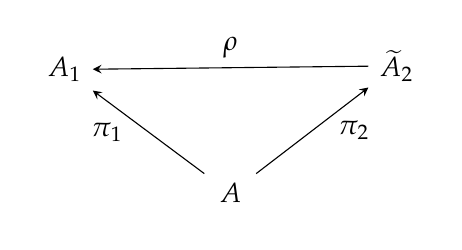
\begin{tikzpicture}
		\matrix (m) [matrix of math nodes,row sep=3em,column sep=4em,minimum width=2em]
		{
			A_1  & & \widetilde{A}_2 \\ 
			& A & \\};
		\path[-stealth]
		(m-1-3) edge node [above] {$\rho$} (m-1-1)
		(m-2-2) edge node [left]  {$\pi_1~~$} (m-1-1)
		(m-2-2) edge node [right] {$~~\pi_2$} (m-1-3);
		\end{tikzpicture}
		\\ 	
	\end{itemize}
	There is the natural equivalence of the categories $A_0:\mathfrak{FinCov}$-$\sX \cong \mathfrak{FinCov}$-$A$.
	
\end{cor}
\begin{proof}
 From the Theorem \ref{ctr_fin_thm} it follows that there is a one-to-one correspondence between objects of $\mathfrak{FinCov}$-$\sX$ and objects of  $\mathfrak{FinCov}$-$A$ given by
	$$
	\left(p:\widetilde{\sX} \to \sX \right) \mapsto 	A_0\left( p\right) :   A_0\left( \sX\right)    \hookto A_0\left( \widetilde{\sX}\right)
	$$
	where $A_0\left(p\right)$ is given by the Definition \ref{ctr_funct_not_defn}. If $p_1:\widetilde{\sX}_1 \to \sX$ and $p_2:\widetilde{\sX}_2 \to \sX$ are objects of $\mathfrak{FinCov}$-$\sX$ and $p: \widetilde{\sX}_1 \to \widetilde{\sX}_2$ is a morphism of $\mathfrak{FinCov}$-$\sX$ then from the Theorem \ref{ctr_fin_thm} it turns out that $p$ is a transitive finite-fold covering. From the equation \ref{ctr_ff_funct_not_eqn} it follows that $p$ corresponds to the *-homomorphism
	\be\label{ctr_c_funct_lem_eqn}
	A_0\left(p \right):  A_0\left( \widetilde{\sX}_2\right)    \to A_0\left( \widetilde{\sX}_1\right).
	\ee
	So one has a functor from  $\mathfrak{FinCov}$-$\sX$ to  $\mathfrak{FinCov}$-$A$. Let us define the inverse  functor. From the Theorem \ref{ctr_fin_thm} it follows that any object $\pi: A_0\left( \sX\right) \hookto A_0\left( \widetilde{\sX}\right)$ of $\mathfrak{FinCov}$-$A$ corresponds to a transitive finite-fold covering $p: \widetilde{\sX} \to \sX$ such that $\pi = A_0\left(p \right)$. If $A_0\left(p_1 \right): A_0\left( {\sX}\right)\to  A_0\left( \widetilde{\sX}_1\right) $ and $A_0\left(p_2 \right): A_0\left( {\sX}\right)\to A_0\left( \widetilde{\sX}_2\right)$ are objects of $\mathfrak{FinCov}$-$A$  and $\pi: A_0\left( \widetilde{\sX}_2\right)    \to A_0\left( \widetilde{\sX}_1\right)$ is a *-homomorphism such that $A_0\left(p_1\right) = \pi \circ A_0\left(p_2\right)$ then $\pi$ corresponds to a continuous map $p: \widetilde{\sX}_1 \to \widetilde{\sX}_2$ such than $p_1= p \circ p_2$. So one has the inverse functor from   $\mathfrak{FinCov}$-$A$ to $\mathfrak{FinCov}$-$\sX$.
\end{proof}






\subsection{Induced representation}\label{ctr_induced_finite_sec}
\paragraph*{} 
Let $\A_{\mathrm{fin}}= \bigoplus_{j=1}^{K}\mathbb{M}_{n_{j}}\left( \C\right)$.
Let $\left(\A, \H, D\right)$ be a spectral triple given by \eqref{ctr_sp_eqn}, i.e.
\be\label{ctr_sp_tr_eqn}
\begin{split}
\left(\A, \H, D\right) = \\=\left( \Coo\left( M\right) \otimes \A_{\mathrm{fin}}, L^2\left( M, S\right)\otimes \C^N,\slashed D_1 \otimes \chi_2 + \Id_{L^2\left( M, S\right)} \otimes D_2\right). 
\end{split}
\ee

If $p: \widetilde{M} \to M$ is a transitive covering and $\pi: C\left(M \right)\to C\left(  \widetilde{M}\right)$ corresponds to $p$   then from the Theorem \ref{ctr_fin_thm} it turns out that 
\be\label{ctr_sp_cov_eqn}
\left( C\left(M \right) \otimes\A_{\mathrm{fin}} ,C\left(  \widetilde{M}\right)  \otimes\A_{\mathrm{fin}}, G\left(\widetilde{M}~|~ M \right), \pi  \right)
\ee is a a noncommutative finite-fold  covering. Indeed \eqref{ctr_sp_cov_eqn} is an unital covering because both  $C\left(M \right)\otimes \A_{\mathrm{fin}}$ and $C\left(\widetilde{M} \right)\otimes \A_{\mathrm{fin}}$ are unital algebras.
Similarly to \ref{comm_induced_finite_sec} consider a smooth partition of unity \eqref{comm_sum_1_eqn}, i.e.

\be\label{ctr_sum_1_eqn}
\begin{split}
	1_{C\left(\widetilde{ M}\right) }= \sum_{g \in G}\sum_{\a \in \mathscr A}g\left(  \widetilde{e}_\a\otimes 1_{\A_{\mathrm{fin}}}\right) ^2= \sum_{\widetilde{\a} \in \widetilde{\mathscr A}}\left( \widetilde{e}_{\widetilde{\a}}\otimes 1_{\A_{\mathrm{fin}}}\right)^2,
	\\
	\left( g\left( \widetilde{e}_{\widetilde{\a}}\otimes 1_{\A_{\mathrm{fin}}}\right) \right)\left(   \widetilde{e}_{\widetilde{\a}}\otimes 1_{\A_{\mathrm{fin}}}\right) = 0; \text{ for any nontrivial } g \in G.\\1_{C\left(\widetilde{ M}\right) } =\sum_{{\widetilde{\a} \in {\widetilde{\mathscr A}}}}\widetilde{e}_{\widetilde{\a}}\otimes 1_{\A_{\mathrm{fin}}}\left\rangle \right\langle \widetilde{e}_{\widetilde{\a}}\otimes 1_{\A_{\mathrm{fin}}},
	\\
	\left\langle \widetilde{e}_{\widetilde{\a}'}\otimes 1_{\A_{\mathrm{fin}}}, \widetilde{e}_{\widetilde{\a}''}\otimes 1_{\A_{\mathrm{fin}}} \right\rangle 	\in \Coo\left( M\right) 	
\end{split}
\ee
From the  equations \ref{ctr_sum_1_eqn} it turns out that
\be\label{str_sum1_eqn}
\begin{split}
	1_{C\left(\widetilde{ M}\right) \otimes \A_{\mathrm{fin}}}= \sum_{g \in G}\sum_{\a \in \mathscr A}g\widetilde{e}^2_\a \otimes 1_{\A_{\mathrm{fin}}}= \sum_{\widetilde{\a} \in \widetilde{\mathscr A}}\left( \widetilde{e}_{\widetilde{\a}}\otimes 1_{\A_{\mathrm{fin}}}\right)^2~~,\\
	\left( g\widetilde{e}_{\widetilde{\a}}\otimes 1_{\A_{\mathrm{fin}}}\right)  \left( \widetilde{e}_{\widetilde{\a}}\otimes 1_{\A_{\mathrm{fin}}}\right) = 0; \text{ for any nontrivial } g \in G.\\1_{C\left(\widetilde{ M}\right)\otimes 1_{\A_{\mathrm{fin}}} } =\sum_{{\widetilde{\a} \in {\widetilde{\mathscr A}}}}\widetilde{e}_{\widetilde{\a}}\otimes 1_{\A_{\mathrm{fin}}}\left\rangle \right\langle \widetilde{e}_{\widetilde{\a}}\otimes 1_{\A_{\mathrm{fin}}},\\
	\left\langle \widetilde{e}_{\widetilde{\a}'}\otimes 1_{\A_{\mathrm{fin}}}, \widetilde{e}_{\widetilde{\a}''} \otimes 1_{\A_{\mathrm{fin}}}\right\rangle_{C\left(  \widetilde{M}\right) \otimes \A_{\mathrm{fin}}} =	\left\langle \widetilde{e}_{\widetilde{\a}'}, \widetilde{e}_{\widetilde{\a}''}\right\rangle_{C\left(  \widetilde{M}\right)}\otimes  1_{\A_{\mathrm{fin}}}	\in \Coo\left( M\right) \otimes {\A_{\mathrm{fin}}}.	
\end{split}
\ee
The set $\left\{\widetilde{e}_{\widetilde{\a}}\otimes  1_{\A_{\mathrm{fin}}}\right\}_{\widetilde{\a}\in \widetilde{\mathscr A}}$ is $G$-invariant, i.e.
\be\label{ctr_a_g_inv}
G\left\{\widetilde{e}_{\widetilde{\a}}\otimes  1_{\A_{\mathrm{fin}}}\right\}_{\widetilde{\a}\in \widetilde{\mathscr A}}=\left\{\widetilde{e}_{\widetilde{\a}}\otimes  1_{\A_{\mathrm{fin}}}\right\}_{\widetilde{\a}\in \widetilde{\mathscr A}}
\ee
Any  element in $\widetilde{\xi}\in \Ga\left(\widetilde{M},\widetilde{S}\otimes \C^N \right)\cong \Ga\left(\widetilde{M},\widetilde{S}\right)\otimes \C^N $ can be represented as
\begin{equation}\label{ctr_xi_repr}
\widetilde{\xi} = \sum_{g \in G} \sum_{\a \in \mathscr A} \left( \left( g \widetilde{e}^2_\a\right)\otimes 1_{\A_{\mathrm{fin}}}\right)   \widetilde{\xi}.
\end{equation}
From $\left(g \widetilde{e}_\a \right)^2= g\widetilde{e}_\a e_\a$ and $$\supp ~\left( g\widetilde{e}_\a\right)  \widetilde{\xi}\subset \supp~g\widetilde{e}_\a \subset g \widetilde{\mathcal U}_\a$$    we can establish a $\C$-linear isomorphism
\begin{equation}\label{ctr_smooth_iso_eqn}
\begin{split}
\varphi:\Ga\left(\widetilde{M},\widetilde{S} \right)\otimes \C^N  \xrightarrow{\approx} \left( C\left(\widetilde{M} \right)\otimes\A_{\mathrm{fin}}   \right) \otimes_{C\left( M\right)\otimes \A_{\mathrm{fin}}}\left(   \Ga\left(M,S \right)\right) \otimes \C^N,\\
\widetilde{\xi}=   \sum_{j=1}^N \widetilde{\xi}_{j} \otimes \mathfrak{e}_j=
 \sum_{g \in G} \sum_{\a \in \mathscr A}\left(  \left( g \widetilde{e}_\a\right) \otimes 1_{\A_{\mathrm{fin}}} \right) \left(  \left( g \widetilde{e}_\a\right) \otimes 1_{\A_{\mathrm{fin}}} \right)\left( \sum_{j=1}^N \widetilde{\xi}_{j} \otimes \mathfrak{e}_j\right)\mapsto \\
\mapsto \sum_{g \in G} \sum_{\a \in \mathscr A}  \left(  \left( g \widetilde{e}_\a\right) \otimes 1_{\A_{\mathrm{fin}}} \right)  \otimes \mathfrak{desc}\left( \left(  \left( g \widetilde{e}_\a\right) \otimes 1_{\A_{\mathrm{fin}}} \right)  \sum_{j=1}^N \widetilde{\xi}_{j} \otimes \mathfrak{e}_j\right) 
\end{split}
\end{equation}%\label{ctr_fin_tens_eqn}
where $\mathfrak{desc}$ means $p$-descent (cf. Definition \ref{top_lift_desc_defn}). Since  $\Ga\left(M,S \right)\otimes \C^N$, (resp. $\Ga\left(\widetilde{M},\widetilde{S} \right)\otimes \C^N$) is dense in $L^2\left(M,S \right)\otimes \C^N$, (resp. $L^2\left(\widetilde{M},\widetilde{S} \right)\otimes \C^N$) the isomorphism \eqref{ctr_smooth_iso_eqn} can be uniquely extended up to $\C$-isomorphism
\be\label{ctr_tensor_iso_eqn}
\begin{split}
\varphi:L^2\left(\widetilde{M},\widetilde{S} \right) \otimes \C^N\xrightarrow{\approx}\\ \left( C\left(\widetilde{M} \right)\otimes\A_{\mathrm{fin}}\right)   \otimes_{C\left( M\right)\otimes \A_{\mathrm{fin}}} \left(  L^2\left(M,S \right)\otimes \C^N\right) .
\end{split}
\ee
 There is the diagonal inclusion of matrix algebras
\be\label{ctr_matr_inc_eqn}
\phi: \A_{\mathrm{fin}}= \bigoplus_{j=1}^{K}\mathbb{M}_{n_{j}}\left( \C\right)\hookto \mathbb{M}_{n_1+...+n_K}\left(\C \right).
\ee  
Let us define following elements
\bean
{\xi}  =\sum_{j=1}^N {\xi}_{j} \otimes \mathfrak{e}_j, ~ {\eta}  = \sum_{j=1}^N \widetilde{\eta}_{j} \otimes \mathfrak{e}_j\in \Ga\left({M},{S} \right)\otimes \C^N;\\
\widetilde{a} = \sum_{\substack{j = 1\\ k=1}}^L\widetilde{a}_{jk}\otimes\mathfrak{e}_{jk},~\widetilde{b} = \sum_{\substack{j = 1\\ k=1}}^L\widetilde{b}_{jk}\otimes\mathfrak{e}_{jk}\in C\left( \widetilde{M}\right)\otimes \phi\left( \A_{\mathrm{fin}} \right) 
\eean
where $L = n_1+...+n_K$ and  $\mathfrak{e}_{jk}\in  \mathbb{M}_{n_1+...+n_K}\left(\C \right)$ means the $j,k$-elementary matrix (cf. Definition \ref{elementary_defn}), and $\phi$ is given by \eqref{ctr_matr_inc_eqn}. Both $\widetilde{a}$ and $\widetilde{b}$ can be regarded as elements of $\A_{\mathrm{fin}}$ an we will do it in the following text.
If $\widetilde{a}_{\widetilde{\a}}=\widetilde{e}^2_{\widetilde{\a}}$ then
	$$
	1_{C\left( \widetilde{M}\right) }= \sum_{\widetilde{\a}\in \widetilde{\mathscr A}}\widetilde{a}_{\widetilde{\a}}= \sum_{\widetilde{\a}\in \widetilde{\mathscr A}}\widetilde{e}^2_{\widetilde{\a}}.
	$$
	One has 
	\bean
	\left\langle \widetilde{a}, \widetilde{b} \right\rangle_{C\left({M}\right)  \otimes \A_{\mathrm{fin}}}= \sum_{\widetilde{\a} \in \widetilde{\mathscr A}} \left\langle \widetilde{a}_{\widetilde{\a}}\widetilde{a}, \widetilde{b} \right\rangle_{C\left(\widetilde{M}\right)  \otimes \A_{\mathrm{fin}}}= \sum_{\substack{j = 1\\k =1\\l=1}}^L \sum_{\widetilde{\a} \in \widetilde{\mathscr A}} \left\langle \widetilde{a}_{\widetilde{\a}}\widetilde{a}_{lj}, \widetilde{b}_{lk} \right\rangle_{C\left(\widetilde{M}\right)} \otimes \mathfrak{e}_{jk}=\\=
	\sum_{\substack{j = 1\\k =1\\l=1}}^n \sum_{\widetilde{\a} \in \widetilde{\mathscr A}}\mathfrak{desc} \left(  \widetilde{a}_{\widetilde{\a}}\widetilde{a}^*_{lj} \widetilde{b}_{lk} \right) \otimes \mathfrak{e}_{jk}.
	\eean
If  $\H'=L^2\left({M},{S} \right)$ and ${\H} = L^2\left(\widetilde{M},\widetilde{S} \right) \otimes \C^N$.  then  the given by \ref{ind_act_form_eqn} scalar product $\left(\cdot, \cdot \right)_{\text{ind}}$ on  $\left( C\left(\widetilde{M} \right)\otimes \A_{\mathrm{fin}} \right)  \otimes\left(  L^2\left({M},{S}, \mu\right)\otimes \C^N\right) $ satisfies to the following equation
\begin{equation}\label{ctr_hilb_prod_eqn}
\begin{split}
\left( \widetilde{a} \otimes \xi ,    \widetilde{b} \otimes \eta\right)_{\text{ind}}= \left(\xi, \left\langle \widetilde{a}, \widetilde{b}\right\rangle_{C\left(\widetilde{M} \right)\otimes \A_{\mathrm{fin}} } \eta \right)_{\H}=
\\
=\sum_{\widetilde{\a}\in \widetilde{\mathscr A}}\left(\xi, \left\langle \widetilde{a}_{\widetilde{\a}}\widetilde{a}, \widetilde{b}\right\rangle_{C\left(\widetilde{M} \right)\otimes \A_{\mathrm{fin}} } \eta \right)_{\H}=
\\
= \left(\xi,\left(  \sum_{\substack{j = 1\\k =1\\l=1}}^L \sum_{\widetilde{\a} \in \widetilde{\mathscr A}}\mathfrak{desc} \left(  \widetilde{a}_{\widetilde{\a}}\widetilde{a}^*_{lj} \widetilde{b}_{lk} \right) \otimes \mathfrak{e}_{jk}\right)  \eta\right)_{\H}=
\\
=	\left(\sum_{p=1}^{N}   {\xi}_{p} \otimes \mathfrak{e}_p,\left(  \sum_{\substack{j = 1\\k =1\\l=1}}^L\sum_{\widetilde{\a} \in \widetilde{\mathscr A}}\mathfrak{desc} \left(  \widetilde{a}_{\widetilde{\a}}\widetilde{a}^*_{lj} \widetilde{b}_{lk} \right) \otimes \mathfrak{e}_{jk}\right)  \left( \sum_{p=1}^{N}  {\eta}_{p} \otimes \mathfrak{e}_p\right) \right)_{\H}=
\\
=\sum_{\widetilde{\a} \in \widetilde{\mathscr A}}\sum_{\substack{j = 1\\k =1\\l=1}}^L\left(\xi_j, \mathfrak{desc} \left(  \widetilde{a}_{\widetilde{\a}}\widetilde{a}^*_{lj} \widetilde{b}_{lk} \right) \eta_k\right)_{\H'} =
\\
= \sum_{\widetilde{\a} \in \widetilde{\mathscr A}}\sum_{\substack{j = 1\\k =1\\l=1}}^L \int_M \left( \xi_j, \mathfrak{desc} \left(  \widetilde{a}_{\widetilde{\a}}\widetilde{a}^*_{lj} \widetilde{b}_{lk} \right) \eta_k\right)_{x} d\mu=
\\
=\sum_{\widetilde{\a} \in \widetilde{\mathscr A}}\sum_{\substack{j = 1\\k =1\\l=1}}^L \int_{\widetilde{M}}
\left( \lift_{\widetilde{\sU}_{\widetilde{\a}}}\left(\widetilde{e}_{\widetilde{\a}}\xi_j \right)_{\widetilde{x}},  \widetilde{a}^*_{lj} \widetilde{b}_{lk} ~\lift_{\widetilde{\sU}_{\widetilde{\a}}}\left(\widetilde{e}_{\widetilde{\a}}\eta_k \right)_{\widetilde{x}}\right)_{\widetilde{x}}d \widetilde{   \mu} =
\\
=\sum_{\substack{j = 1\\k =1\\l=1}}^L \int_{\widetilde{M}}
\left( \widetilde{a}_{lj} \lift_p\left(\xi_l \right)_{\widetilde{x}},   \widetilde{b}_{lk} ~\lift_p\left(\eta_k \right)_{\widetilde{x}}\right)_{\widetilde{x}}d \widetilde{   \mu}
=
\\
= \left( \widetilde{a}~ \lift_p\left(\xi \right),  \widetilde{b} ~\lift_p\left(\eta \right)\right)_{L^2\left(\widetilde{M},\widetilde{S} \right)\otimes\C^N}= \left( \widetilde{a} \otimes \xi ,    \widetilde{b} \otimes \eta\right)_{L^2\left(\widetilde{M},\widetilde{S} \right)\otimes\C^N}. \\
\end{split} 
\end{equation}
The equation \eqref{ctr_hilb_prod_eqn} means that $\left(\cdot, \cdot \right)_{\text{ind}}= \left(\cdot, \cdot \right)_{L^2\left(\widetilde{M},\widetilde{S} \right)}$, and taking into account the dense inclusion $C\left(\widetilde{M} \right) \otimes_{C\left(M \right) } \Ga\left( M, S\right) \subset L^2\left(\widetilde{M},\widetilde{S} \right)$ with respect to the Hilbert norm of $L^2\left(\widetilde{M},\widetilde{S}\right)\otimes\C^N $. one concludes that the space of induced representation coincides with $L^2\left(\widetilde{M},\widetilde{S}\right)$. 
If $\varphi$ is the extension of the given by \eqref{ctr_smooth_iso_eqn} map and  $\widetilde{a} \in C_0\left( \widetilde{M}\right)$ then following condition holds
\be\label{ctr_fin_act_eqn}
\varphi\left( \widetilde{a}  \widetilde{\xi}\right) =\sum_{g \in G} \sum_{\a \in \mathscr A} \widetilde{a} \left( g  \widetilde{e}_\a\right)   \otimes \mathfrak{desc}\left(\left( g\widetilde{e}_\a\right)  \widetilde{\xi}\right) 
\ee
where the left part of \eqref{ctr_fin_act_eqn} is relevant to the natural action of $C_0\left(\widetilde{M}\right)$ on $ L^2\left(\widetilde{M},\widetilde{S} \right)$,  the right part  is consistent with \eqref{ind_act_form_eqn}. It means that induced representation is given by the well known action $C\left(\widetilde{M}\right) \times L^2\left(\widetilde{M},\widetilde{S} \right) \to L^2\left(\widetilde{M},\widetilde{S} \right)$. So one has the following lemma.	From \eqref{ctr_hilb_prod_eqn} it follows that the Hilbert scalar product of the induced representation it the  Hilbert scalar product of the tensor product, i.e.
	\be\label{ctr_cs_pr_eqn}
	\begin{split}
	\left(\widetilde{\xi} \otimes x, \widetilde{\eta} \otimes y\right)_{L^2\left(\widetilde{M},\widetilde{S} \right) \otimes \C^N} = \left(\widetilde{\xi} , \widetilde{\eta} \right)_{L^2\left(\widetilde{M},\widetilde{S} \right)}\left(x,y \right)_{\C^N} \\
	\text{where} \quad \widetilde{\xi} \otimes x, \widetilde{\eta} \otimes y \in L^2\left(\widetilde{M},\widetilde{S} \right) \otimes \C^N	\end{split}
	\ee
	

\begin{lemma}\label{ctr_ind_lem}
	If the representation  $\widetilde{\rho}: C\left(\widetilde{M}\right) \otimes \A_{\mathrm{fin}} \to  B\left( \widetilde{   \H}\right)  $ is induced by the pair $$\left(C\left(M \right)\otimes \A_{\mathrm{fin}} \to B\left(  L^2\left(M,S \right)\right)\otimes \C^N ,\left(C\left(M \right) \otimes \A_{\mathrm{fin}}, C\left( \widetilde{M}\right) \otimes \A_{\mathrm{fin}}, G \right)  \right)$$ (cf. Definition \ref{induced_repr_defn}) where $G=G\left( \left.\widetilde{M}~\right|M\right)$ then there is the isomorphism of Hilbert spaces $\widetilde{   \H}\cong L^2\left(\widetilde{M},\widetilde{S} \right)\otimes \C^N$ with scalar product is given by \eqref{ctr_cs_pr_eqn}.
\end{lemma}
For any $\widetilde{a} \in \Coo_0\left(\widetilde{M} \right)\otimes\A_{\mathrm{fin}}$ following condition holds 
\bean
\widetilde{a} = \sum_{\substack{j = 1\\ k=1}}^L \widetilde{a}_{jk} \otimes \mathfrak{e}_{jk},\text{ where } \widetilde{a}_{jk} \in \Coo\left(\widetilde{M} \right);\\
\left( \widetilde{e}_{\widetilde{\a}'}\otimes 1_{\A_{\mathrm{fin}}}\right) \widetilde{a}\left( \widetilde{e}_{\widetilde{\a}''}\otimes 1_{\A_{\mathrm{fin}}}\right)  = \sum_{\substack{j = 1\\ k=1}}^n \widetilde{e}_{\widetilde{\a}'}\widetilde{a}_{jk}\widetilde{e}_{\widetilde{\a}''}\otimes \mathfrak{e}_{jk}
\in \Coo\left(\widetilde{M} \right)\otimes\A_{\mathrm{fin}},
\eean
hence one has
\bean
\left\langle \widetilde{e}_{\widetilde{\a}'}\otimes 1_{\A_{\mathrm{fin}}}~,~~\widetilde{a}\left( \widetilde{e}_{\widetilde{\a}''}\otimes 1_{\A_{\mathrm{fin}}}\right) \right\rangle_{C\left(\widetilde{M} \right)\otimes\A_{\mathrm{fin}}}  =\\= \sum_{\substack{j = 1\\ k=1}}^n\mathfrak{desc}\left(\widetilde{e}_{\widetilde{\a}'}\widetilde{a}_{jk}\widetilde{e}_{\widetilde{\a}''} \right) \otimes \mathfrak{e}_{jk} \in \Coo\left(M \right)\otimes\A_{\mathrm{fin}}.
\eean
Otherwise form $\widetilde{a} \notin \Coo\left(\widetilde{M} \right)\otimes\A_{\mathrm{fin}}$ it turns out that 
$
\exists \widetilde{\a} \in \widetilde{\mathscr A}, j,k \in \left\{1,...,n\right\}~~ \widetilde{e}^2_{\widetilde{\a}} \widetilde{a}_{jk} \notin \Coo\left(\widetilde{M} \right)$, hence
\bean
\left\langle \widetilde{e}_{\widetilde{\a}}~,~~\widetilde{a}\widetilde{e}_{\widetilde{\a}}\right\rangle_{C\left(\widetilde{M} \right)}  = \sum_{\substack{j = 1\\ k=1}}^n\mathfrak{desc}\left(\widetilde{e}^2_{\widetilde{\a}}\widetilde{a}_{jk} \right) \notin \Coo\left({M} \right)\Rightarrow\\
\Rightarrow \left\langle \widetilde{e}_{\widetilde{\a}'}\otimes 1_{\A_{\mathrm{fin}}}~,~~\widetilde{a}\left( \widetilde{e}_{\widetilde{\a}''}\otimes 1_{\A_{\mathrm{fin}}}\right) \right\rangle_{C\left(\widetilde{M} \right)\otimes\A_{\mathrm{fin}}}\notin \Coo\left(\widetilde{M} \right)\otimes\A_{\mathrm{fin}}
\eean
Summarize above equations one concludes
\bean
\Coo\left(\widetilde{M} \right)\otimes\A_{\mathrm{fin}}=\\
= \left\{\widetilde{a}\in C\left(\widetilde{M} \right)\otimes\A_{\mathrm{fin}}~|~  \left\langle \widetilde{e}_{\widetilde{\a}'}\otimes 1_{\otimes\A_{\mathrm{fin}} }~,~~\widetilde{a}\left( \widetilde{e}_{\widetilde{\a}''}\otimes 1_{\A_{\mathrm{fin}}} \right) \right\rangle_{C\left({M} \right)}\right.\in \\ \left.\in \Coo\left( M\right)\otimes\A_{\mathrm{fin}}; ~ \forall \widetilde{\a}', \widetilde{\a}'' \in \widetilde{\mathscr A} \right\}.
\eean
From the Lemma \ref{smooth_matr_lem} it turns out that
\begin{itemize}
	\item The unital noncommutative finite-fold covering $\left(C\left({M} \right), C\left(\widetilde{M} \right), G\left( \widetilde{M}~|~M \right)\right) $ is {smoothly invariant} (cf. Definition \ref{smooth_defn}),
	\item 
	\be\label{ctr_smooth_matr_eqn}
	\Coo\left(\widetilde{M} \right)\otimes \A_{\mathrm{fin}}  = C\left(\widetilde{M}\otimes \A_{\mathrm{fin}} \right)\bigcap 
	\mathbb{M}_{\left|\widetilde{\mathscr A} \right| }\left( \Coo\left( M\right) \otimes \A_{\mathrm{fin}}\right).
	\ee 	
\end{itemize}

\subsection{Inverse image of the Dirac operator}
There are 
following isomorphisms
\bean
C\left(M \right)  \otimes \A_{\mathrm{fin}} \cong  C_0\left(M, \left\{\C_x \otimes \otimes \A_{\mathrm{fin}}\right\}_{x \in \sX}, C\left(M \right)  \otimes \A_{\mathrm{fin}}\right) ,\\
\Ga\left(M, \sS \right) \otimes \C^N= C_0\left(M, \left\{\sS_x \otimes \C^N\right\}, \Ga\left(M, \sS \otimes \C^N \right) \right) 
\eean
where the notation of the Definition \ref{top_cc_c0_defn} is used.
Similarly to the example \ref{top_vb_lift_desc_exm} it follows that there is the sheaf of continuous sections
$$
\mathscr C \left(M, \left\{\sS_x \otimes \C^N\right\}, \Ga\left(M, \sS^N \otimes \C^N \right)  \right). 
$$
Otherwise there is the dense subspace of smooth sections 
$$
\Ga^\infty\left(M, \sS \otimes \C^N \right) \subset \Ga\left(M, \sS \otimes \C^N \right)
$$
which induces the dense subsheaf 
\bean
\mathscr C^\infty \left(M, \left\{\sS_x \otimes \C^N \right\},\Ga\left(M, \sS\otimes \C^N \right) \right)\subset \mathscr C \left(M, \left\{\sS_x\otimes \C^N\right\}, \Ga\left(M, \sS \otimes \C^N\right) \right)
\eean
of smooth sections.
If $p : \widetilde{M} \to M$ is a covering then
\bean
\mathscr C^\infty \left(\widetilde{M}, \left\{\SS_{\widetilde{x}}\otimes \C^N\right\}_{\widetilde{x} \in \widetilde{M}}, \Ga\left(\widetilde{M}, \widetilde{\sS} \otimes \C^N\right) \right) = p^{-1} \mathscr C^\infty \left(M, \left\{\sS_x\otimes \C^N\right\}_{x \in M}, \Ga\left(M, \sS \otimes \C^N\right) \right)
\eean
If $D$ is Dirac operator of the spectral triple \ref{ctr_sp_tr_eqn} and $a \in \Coo\left(M \right)  \otimes \A_{\mathrm{fin}}$ then  one has
\be\label{ctr_d_hom_eqn}
\begin{split}
a, D \in \mathscr Hom \left(\mathscr S, \mathscr S \right)
\\
\text{where } \mathscr S = \mathscr C^\infty \left(M, \left\{\sS_x \otimes \C^N\right\}, \Ga\left(M, \sS \otimes \C^N \right) \right)
\end{split}
\ee	



\subsection{Lift of the Dirac operator}\label{ctr_d_sec}
\paragraph*{}
For any $\widetilde{a}=\sum_{\substack{j = 1\\ k=1}}^n \widetilde{a}_{jk} \otimes \mathfrak{e}_{jk} \in \Coo\left(\widetilde{M} \right)\otimes \A_{\mathrm{fin}}$ following condition holds
\bean
\widetilde{a} = \sum_{\widetilde{\a}\in \widetilde{\mathscr A}} \widetilde{\ga}_{\widetilde{\a}}= \sum_{\widetilde{\a}\in \widetilde{\mathscr A}} \widetilde{\psi}_{\widetilde{\a}}\widetilde{\phi}_{\widetilde{\a}}; \text{ where } \widetilde{\phi}_{\widetilde{\a}}= \widetilde{e}_{\widetilde{\a}}\otimes 1_{\A_{\mathrm{fin}}},\\ \widetilde{\psi}_{\widetilde{\a}}= \sum_{\substack{j = 1\\ k=1}}^n \widetilde{e}_{\widetilde{\a}}\widetilde{a}_{jk} \otimes \mathfrak{e}_{jk} = \sum_{\substack{j = 1\\ k=1}}^n \widetilde{\psi}_{\widetilde{\a}jk}  ,~ \widetilde{\ga}_{\widetilde{\a}}=\widetilde{a}_{\widetilde{\a}}\left( \widetilde{e}^2_{\widetilde{\a}}\otimes 1_{\A_{\mathrm{fin}}}\right) .
\eean
Denote by $\Om^1_{D}$  the {module of differential forms associated} with the spectral triple given by \eqref{ctr_sp_tr_eqn} (cf. Definition \ref{ass_cycle_defn}). Denote by 
\bean
{\phi}_{\widetilde{\a}} = \mathfrak{desc} \left(\widetilde{\phi}_{\widetilde{\a}} \right)=\mathfrak{desc} \left(\widetilde{e}_{\widetilde{\a}} \right) \otimes 1_{\A_{\mathrm{fin}}}, \\ {\psi}_{\widetilde{\a} jk} = \mathfrak{desc} \left(\widetilde{\psi}_{\widetilde{\a}jk} \right)=  \mathfrak{desc}\left( \widetilde{e}_{\widetilde{\a}}\widetilde{a}_{jk}\right) \otimes \mathfrak{e}_{jk},\\
{\psi}_{\widetilde{\a}}=\sum_{\substack{j = 1\\ k=1}}^n {\psi}_{\widetilde{\a} jk}\otimes \mathfrak{e}_{jk},\\  {\ga}_{\widetilde{\a}} = \mathfrak{desc} \left(\widetilde{\ga}_{\widetilde{\a}} \right)\in \Coo\left({M} \right)\otimes \A_{\mathrm{fin}}.
\eean 
Similarly to \eqref{comm_matr_x_eqn} one can prove
\begin{equation}\label{ctr_comm_eqn}
\begin{split}
\left[ { D}, \sum_{\substack{j = 1\\ k=1}}^n {e}_{\widetilde{\a}}{a}_{jk} \otimes \mathfrak{e}_{jk} \right]\left( {e}_{\widetilde{\a}}\otimes 1_{\A_{\mathrm{fin}}}\right) = \left( {e}_{\widetilde{\a}}\otimes 1_{\A_{\mathrm{fin}}}\right)\left[ { D}, \sum_{\substack{j = 1\\ k=1}}^n {e}_{\widetilde{\a}}{a}_{jk} \otimes \mathfrak{e}_{jk} \right]
\end{split}
\end{equation}
or, equivalently
\begin{equation}\nonumber
\begin{split}
\left[ { D}, {\psi}_{\widetilde{\a}} \right]{\phi}_{\widetilde{\a}} = \phi_{\widetilde{\a}}\left[ { D},{\psi}_{\widetilde{\a}} \right]
\end{split}
\end{equation}

Let us define a $\C$-linear map
\bean
\nabla: \Coo\left(\widetilde{M} \right)\otimes \A_{\mathrm{fin}} \to \left( \Coo\left(\widetilde{M} \right)\otimes \A_{\mathrm{fin}}\right) \otimes_{\Coo\left({M} \right)\otimes \A_{\mathrm{fin}}}\Om^1_{ D},\\
\widetilde{a} \mapsto \sum_{\widetilde{\a}\in \widetilde{\mathscr A}}\left(  \widetilde{\phi}_{\widetilde{\a}} \otimes \left[ D, {\psi}_{\widetilde{\a}}  \right] +\widetilde{\psi}_{\widetilde{\a}} \otimes \left[ D, {\phi}_{\widetilde{\a}}   \right] \right) 
\eean
For any $a \in \Coo\left({M} \right)\otimes \A_{\mathrm{fin}}$ following condition holds
\bean
\nabla\left(\widetilde{a}a \right)=  \sum_{\widetilde{\a}\in \widetilde{\mathscr A}}\left(  \widetilde{\phi}_{\widetilde{\a}} \otimes \left[ D, {\psi}_{\widetilde{\a}} a  \right] +\widetilde{\psi}_{\widetilde{\a}}a \otimes \left[ D, {\phi}_{\widetilde{\a}}   \right] \right) =\\= \sum_{\widetilde{\a}\in \widetilde{\mathscr A}} \widetilde{\phi}_{\widetilde{\a}} \otimes \left[ D, {\psi}_{\widetilde{\a}}  \right]a+\widetilde{\phi}_{\widetilde{\a}} \otimes \widetilde{\psi}_{\widetilde{\a}}\left[ D,  a  \right] +\widetilde{\psi}_{\widetilde{\a}} \otimes \left[ D, {\phi}_{\widetilde{\a}}   \right]a=\\= \sum_{\widetilde{\a}\in \widetilde{\mathscr A}}\left(  \widetilde{\phi}_{\widetilde{\a}} \otimes \left[ D, {\psi}_{\widetilde{\a}}   \right] +\widetilde{\psi}_{\widetilde{\a}} \otimes \left[ D, {\phi}_{\widetilde{\a}}  \right] \right) a+
\sum_{\widetilde{\a}\in \widetilde{I}}\widetilde{\phi}_{\widetilde{\a}}\widetilde{\psi}_{\widetilde{\a}}\left[  D,a\right]=
\nabla\left( \widetilde{a}\right) a + \widetilde{a}\otimes  \left[  D,a\right]. 
\eean
The comparison of the above equation and \eqref{conn_triple_eqn} states that $\nabla$ is a connection. If $g \in  G\left( \left.\widetilde{M}~\right|M\right)$ then from $\mathfrak{desc}\left(g\widetilde{\phi}_{\widetilde{\a}}\right) = {\phi}_{\widetilde{\a}} $ and $\mathfrak{desc}\left(g\widetilde{\psi}_{\widetilde{\a}}\right) = {\psi}_{\widetilde{\a}} $ it follows that
\bean
\nabla\left(g\widetilde{a} \right)=  \nabla\left(\sum_{\widetilde{\a}\in \widetilde{I}} \left( g\widetilde{\phi}_{\widetilde{\a}}\right) \left( g\widetilde{\phi}_{\widetilde{\a}}\right)\right)=\\=\sum_{\widetilde{\a}\in \widetilde{I}}\left( g \widetilde{\phi}_{\widetilde{\a}} \otimes \left[ D, {\psi}_{\widetilde{\a}}   \right] +g\widetilde{\psi}_{\widetilde{\a}} \otimes \left[ D, {\phi}_{\widetilde{\a}}   \right] \right)= g \left( \nabla\left(\widetilde{a} \right)\right),  
\eean
i.e. $\nabla$ is  $G$-{equivariant} (cf. \eqref{equiv_conn_eqn}). 
If $\xi \in \Dom~ D$ then following conditions hold
\bean
\supp~\widetilde{\phi}_{\widetilde{\a}} \otimes \left[ D, {\psi}_{\widetilde{\a}}   \right]\xi \in \widetilde{\mathcal{U}}_{\widetilde\a},\\
\supp~\widetilde{\psi}_{\widetilde{\a}} \otimes \left[ D, {\phi}_{\widetilde{\a}}   \right]\xi \in \widetilde{\mathcal{U}}_{\widetilde\a},
\eean
hence one has
\bean
\widetilde{\phi}_{\widetilde{\a}} \otimes \left[ D, {\psi}_{\widetilde{\a}}   \right]\xi = \mathfrak{lift}_{\widetilde{\mathcal{U}}_{\widetilde\a}} \left({\phi}_{\widetilde{\a}}  \left[ D, {\psi}_{\widetilde{\a}}   \right]\xi \right),\\
\widetilde{\psi}_{\widetilde{\a}} \otimes \left[ D, {\phi}_{\widetilde{\a}}   \right]\xi = \mathfrak{lift}_{\widetilde{\mathcal{U}}_{\widetilde\a}} \left({\psi}_{\widetilde{\a}}  \left[ D, {\phi}_{\widetilde{\a}}   \right]\xi \right).
\eean
From \eqref{comm_matr_x_eqn} it turns out $\widetilde{\psi}_{\widetilde{\a}}  \left[ D, {\phi}_{\widetilde{\a}}   \right] =   \left[ D, {\phi}_{\widetilde{\a}}   \right]\widetilde{\psi}_{\widetilde{\a}}$, hence
\bean
\widetilde{\phi}_{\widetilde{\a}} \otimes \left[ D, {\psi}_{\widetilde{\a}}   \right]\xi + \widetilde{\psi}_{\widetilde{\a}} \otimes \left[ D, {\phi}_{\widetilde{\a}}   \right]\xi = \mathfrak{lift}_{\widetilde{\mathcal{U}}_{\widetilde\a}}\left(\left( \left[ D, {\phi}_{\widetilde{\a}}   \right]{\psi}_{\widetilde{\a}}+{\phi}_{\widetilde{\a}}  \left[ D, {\psi}_{\widetilde{\a}}   \right] \right)\xi \right)= \mathfrak{lift}_{\widetilde{\mathcal{U}}_{\widetilde\a}}\left(\left[ D, {\ga}_{\widetilde{\a}}   \right] \xi\right) 
\eean
If $\widetilde{ D}$ is $\left(C\left(M\right) , C\left(\widetilde{M} \right) , G\left(\widetilde{M}~|M \right)   \right)$-lift of $ D$ (cf. Definition \ref{triple_conn_lift_defn})   and $\xi \in \H^\infty$ then 
from \eqref{d_defn_eqn},  $\mathfrak{lift}_{\widetilde{\mathcal{U}}_{\widetilde\a}}\left( {\ga}_{\widetilde{\a}}\right) = \widetilde{\ga}_{\widetilde{\a}}$ and $\sum_{\widetilde{\a}\in \widetilde{\mathscr A}}~ \widetilde{\ga}_{\widetilde{\a}} = \widetilde{a}$. From \eqref{ctr_d_hom_eqn} it follows that there is the $p$-{inverse image} of $D$ (cf. Definition \ref{top_smooth_inv_im_defn}).
 Taking account \eqref{comm_lift_comp_eqn}  one has
\be\nonumber
\begin{split}
	\widetilde{ D}\left(\widetilde{a} \otimes \xi \right)= \sum_{\widetilde{\a}\in \widetilde{\mathscr A}}\left(  \widetilde{\phi}_{\widetilde{\a}} \otimes \left[ D, {\psi}_{\widetilde{\a}}  \right]\xi +\widetilde{\psi}_{\widetilde{\a}} \otimes \left[ D, {\phi}_{\widetilde{\a}}   \right] \xi\right)+ \widetilde{a} \otimes  D\xi =\\=\sum_{\widetilde{\a}\in \widetilde{\mathscr A}}    
	\mathfrak{lift}_{\widetilde{\mathcal U}_{\widetilde{   \a}}}\left( \left[{ D}, {\ga}_{\widetilde{\a}}  \right]\right) \left(1 \otimes \xi\right)  +\widetilde{a} \otimes  D\xi =\\  = \left[p^{-1}D , {\widetilde{a}}   \right]\left(1 \otimes \xi \right)+ \widetilde{a} \otimes  D\xi =\\=
	\left[p^{-1}D , {\widetilde{a}}   \right]\left(1 \otimes \xi \right)+ \widetilde{a}~ p^{-1}D\left( 1  \otimes \xi\right) = p^{-1}D \left(\widetilde{a} \otimes \xi \right),
\end{split}
\ee
where $p^{-1}D$ is the  is the $p$-{inverse image} of $D$.
In result we have.
\be\label{ctr_df_eqn}
\widetilde{ D} = p^{-1}D.
\ee

\subsection{Coverings of spectral triples}
\paragraph*{}
From \eqref{ctr_sum_1_eqn} it turns that 
 $C\left(M \right)\otimes \A_{\mathrm{fin}}$-module $C\left(\widetilde{M} \right)\otimes \A_{\mathrm{fin}}$ is generated by  a finite set $\left\{\widetilde{e}_{\widetilde{\a}}\otimes 1_{\A_{\mathrm{fin}}}\right\}_{\widetilde{\a}\in \widetilde{\mathscr A}}$, i.e.
$$
C\left(\widetilde{M} \right)\otimes \A_{\mathrm{fin}} = \sum_{\widetilde{\a}\in \widetilde{\mathscr A}}  \left( \widetilde{e}_{\widetilde{\a}}\otimes 1_{ \A_{\mathrm{fin}}}\right) ~C(M)\otimes \A_{\mathrm{fin}}.
$$ 
Also from \eqref{ctr_sum_1_eqn} it turns out $\left\langle \widetilde{e}_{\widetilde{\a'}}\otimes 1_{ \A_{\mathrm{fin}}}, \widetilde{e}_{\widetilde{\a''}}\otimes 1_{ \A_{\mathrm{fin}}}\right\rangle_{C\left(\widetilde{M} \right) } \in \Coo\left(M \right)\otimes \A_{\mathrm{fin}}$, i.e.  the set $\left\{\widetilde{e}_{\widetilde{\a}}\otimes 1_{ \A_{\mathrm{fin}}}\right\}_{\widetilde{\a}\in \widetilde{\mathscr A}}$ , satisfies to the condition (a) of the Lemma \ref{smooth_matr_lem}. From \eqref{comm_a_g_inv} it turns out that 
$\left\{\widetilde{e}_{\widetilde{\a}}\otimes 1_{ \A_{\mathrm{fin}}}\right\}_{\widetilde{\a}\in \widetilde{\mathscr A}}$ is $G$-invariant, i.e.
\be\nonumber
G\left\{\widetilde{e}_{\widetilde{\a}}\otimes 1_{ \A_{\mathrm{fin}}}\right\}_{\widetilde{\a}\in \widetilde{\mathscr A}}=\left\{\widetilde{e}_{\widetilde{\a}}\otimes 1_{ \A_{\mathrm{fin}}}\right\}_{\widetilde{\a}\in \widetilde{\mathscr A}}~,
\ee
hence the set $\left\{\widetilde{e}_{\widetilde{\a}}\otimes 1_{ \A_{\mathrm{fin}}}\right\}_{\widetilde{\a}\in \widetilde{\mathscr A}}$ , satisfies to the condition (b) of the Lemma \ref{smooth_matr_lem}. From the Lemma \ref{smooth_matr_lem} it turns out that  the unital noncommutative finite-fold covering $\left(C\left(M \right)\otimes\A_{\mathrm{fin}} , C\left( \widetilde{M}\right)\otimes \A_{\mathrm{fin}} , G \right)$ is {smoothly invariant}. Taking into account the Section \ref{ctr_d_sec}  one has the following theorem. 
\begin{thm}\label{ctr_fin_sp_tr_thm} If $\widetilde{ D}=\lift_p\left(  D\right)$ then the spectral triple $$\left(C^{\infty}\left( \widetilde{M}\right)\otimes \A_{\mathrm{fin}}, L^2\left( \widetilde{M}, \widetilde{S}\right)\otimes \C^N ,\widetilde{ D}= p^{-1}D\right)$$ is the $\left(C\left(M \right)\otimes \A_{\mathrm{fin}} , C\left( \widetilde{M}\right) \otimes \A_{\mathrm{fin}} , G\left( \left.\widetilde{M}~\right|M\right)  \right)$-lift of $$\left(C^{\infty}\left( M\right)\otimes \A_{\mathrm{fin}} , L^2\left( M, S\right)\otimes \C^N , D\right).$$
\end{thm}


\subsection{Unoriented spectral triples}\label{ctr_sp_tr} 
\paragraph*{}
Similarly to the Section \ref{comm_sp_tr} one can define unoriented over $C^*$-algebras with continuous trace. Let $M$ be an unoriented  Riemannian manifold, and let $\widetilde{M} \to M$ be a two listed covering by oriented  Riemannian manifold $\widetilde{M}$ with Spin-structure given by Spin-bundle $\SS$. From the construction of the Section \ref{unoti_defn_sec} it follows that there is the  unoriented spectral triple 
\be\label{ctr_equ}
\left(\Coo\left(M \right)\otimes \A_{\mathrm{fin}}, L^2\left(\widetilde{M}, \widetilde{\SS}\right)^{\Z_2}\otimes \C^N= L^2\left({M},{\SS}\right)\otimes \C^N, D  \right).
\ee

\section{Infinite coverings}\label{ctr_case_sec}
\subsection{Coverings of $C^*$-algebras}

\paragraph*{}




\begin{lemma}\label{ctr_t_a_lem}
		Let $A$ be a separable $C^*$-algebra with continuous trace let $\sX = \hat A$ be the spectrum of $A$. Suppose that $\sX$ is a connected, locally connected, second-countable space.
	Let us consider the situation \ref{comm_t_a_empt} and suppose that 
	\bean
	A = C_0\left(\sX, \left\{A_x\right\}_{x \in \sX}, A \right),\\
	\mathscr C = \left(\sX, \left\{A_x\right\}_{x \in \sX}, A \right)
	\eean
	 and $\mathscr C_0 = A_0$ (cf. Equation \ref{top_res_eqn} and  Definition \ref{top_c_funct_defn}).
	Following conditions hold:
	\begin{enumerate}
		\item[(i)] 	If
		$
		\mathfrak{S}_{ \mathcal{X} } = \left\{p_{\la}:\mathcal{X}_\la \to  \mathcal{X}  \right\}_{\la \in \La}\in \mathfrak{FinTop}
		$
		is  a  topological  finite covering category (cf. Definition \ref{top_sec_defn}) then there is the natural  algebraical  finite covering category (cf. Definition \ref{comp_defn}).
		\begin{equation*}
		\mathfrak{S}_{A } = \left\{\pi_\la=A_0\left( p_{\la}\right) :A  \hookto A_0\left( \mathcal{X}_\la\right) \right\}_{\la \in \La}\in \mathfrak{FinAlg}.
		\end{equation*}
		\item[(ii)] Conversely any directed algebraical  finite covering category
		\begin{equation}
		\mathfrak{S}_{A } = \left\{ \pi_{\la} :A  \hookto A_0\left( \mathcal{X}_\la\right) \right\}_{\la \in \La}\in \mathfrak{FinAlg}.
		\end{equation}
		naturally induces 
		directed topological  finite covering category $$
		\mathfrak{S}_{\mathcal{X}} = \left\{p_{\la}:\mathcal{X}_\la \to \mathcal{X}\right\}_{\la \in \La}\in \mathfrak{FinTop}.$$
		
	\end{enumerate}
	
\end{lemma}
\begin{proof}
	(i)
	One needs check the conditions (a) and (b) of the Definition \ref{comp_defn}.
\begin{enumerate}
	\item[(a)] 	The conditions (a)-(d) of the Definition \ref{compliant_covering_defn}  directly follow from (a)-(d) of the Lemma \ref{comm_comply_lem}.
	\item[(b)] Follows from the Corollary \ref{ctr_functor_cor}.
	
	

\end{enumerate}	
	(ii) From the Theorem \ref{ctr_fin_thm} it turns out that any object $ \pi_\la :A  \hookto A_0\left( \mathcal{X}_\la\right)$ of the category $\mathfrak{S}_{A }$ corresponds to the object $p_\la: \sX_\la \to \sX$ of the category $\mathfrak{S}_{ \mathcal{X}}$, i.e. $p_\la$ is a transitive finite-fold covering. If $\mu, \nu \in \La$ are such that $\mu > \nu$ then from (b) of the Definition \ref{comp_defn} it follows that there is *-homomorphism $\pi: A_0\left( \mathcal{X}_\nu\right)\to A_0\left( \mathcal{X}_\mu\right)$ such that 
	\be\label{ctr_inf_pp_eqn}
	A_0\left( p_\mu\right)= \pi \circ A_0\left( p_\nu\right).
	\ee
	From (a) of the Definition \ref{comp_defn} it turns out that the homomorphism $\pi$ is a noncommutative  finite fold covering, so taking into account the Corollary \ref{ctr_functor_cor} one has the topological finite-fold covering $p: \mathcal{X}_\mu\to \mathcal{X}_\nu$ such that $\pi = A_0\left(p\right)$. From \eqref{ctr_inf_pp_eqn} it follows that $p_\mu = p \circ p_\nu$.
\end{proof}

\begin{lemma}\label{ctr_base_point_lem}
	If	$\mathfrak{S}_{\left(\sX, x_0\right)}= \left\{p_\la:\left( \sX_\la, x^\la_0\right) \to \left( \sX, x_0\right)\right\}_{\la \in \La} \in \mathfrak{FinTop}^{\mathrm{pt}}$ is a pointed topological finite covering category such that for any $\mu > \nu$ there is the unique  pointed  covering $p^\mu_{ \nu}: \left(\sX_{\mu}, x^\mu_0 \right) \to \left(\sX_{\nu}, x^\nu_0 \right)$ then
	\be\label{ctr_base_point_eqn}
	\begin{split}
		\mathfrak{S}_{A } = \\
		=\left\{A_0\left( p_\la\right) : A_0\left(\sX \right)  \hookto A_0\left(\sX_\la \right)\right\}, \left\{A_0\left( p_\nu^\mu\right) : A_0\left(\sX_\nu \right) \hookto A_0\left(\sX_\mu \right)\right\}
	\end{split}
	\ee
	is a {pointed algebraical  finite covering category} (cf. Definition \ref{comp_pt_defn}).
\end{lemma}
\begin{proof}
	According to our construction for any $\mu >\nu$ the category $	\mathfrak{S}_{A }$ contains the unique *-homomorphism from $A_0\left(\sX_\nu \right)$ to $A_0\left(\sX_\mu \right)$. This lemma follows from the Remark \ref{comp_pt_rem}.
\end{proof}

\begin{empt}
	Consider the specialization of \ref{top_poi_alg} such that $\mathscr C = \left(\sX, \left\{A_x\right\}_{x \in \sX}, A\right)$,   $\mathscr C_0 = A_0$, and the given by \eqref{top_alg_cat} category.
	Suppose the space $\H_x$ of the representation \eqref{top_ax_repr_eqn} equals to $\K$ where $\K = \mathbb{M}_n\left(\C\right)$ or $\K = \K\left( L^2\left(\N \right) \right)$. 
	From the Lemma \ref{ctr_base_point_lem} it follows that \eqref{ctr_base_point_eqn} is the pointed algebraical  finite covering category. Let $\left\{b_\la  \right\}_{\la \in \La}$ be a special family (cf. Definition \ref{special_set_defn}). If $\widehat{A} = C^*$-$\varinjlim_{\la \in \La} A_0\left( {\sX}_\la\right)$, $\widehat{x}, \widehat{y} \in \widehat{ A}$ then $\left\{a_\la= \widehat{x}b_\la\widehat{y}\right\} \subset  \widehat{ A} $  then the family $\left\{a_\la= \widehat{x}b_\la\widehat{y}\right\}$ is weakly special (cf. Definition \ref{weakly_spec_defn}).  
	Similarly to \eqref{top_ax_l_eqn} one has	
	\be\nonumber
		\overline{a}_{\overline{x}} = \lim_\la A_b\left( \overline{p}_\la\right)\left( a_\la\right)\left(\overline{x} \right) \in B\left(\H_{p\left(\overline{x}\right)}\right),
		\ee
	indeed $\overline{a}_{\overline{x}} \in \K\left(\H_{p\left(\overline{x}\right)}\right) $ for each $\overline{x} \in \overline{\sX}$.
	Any $\overline a \in A_0\left(\overline{\sX} \right)$ corresponds to a family  $\left\{\overline{a}_{\overline{x}} \in \K\left(\H_{p\left(\overline{x}\right)}\right)\right\}_{\overline{x} \in \overline{\sX}}$ it turns out there is the natural inclusion
	\be\label{ctr_a0_to_d_eqn}
	 A_0\left( \overline{\sX}\right)\subset B\left( \oplus_{\overline{x}\in\overline{\sX}}\H_{\overline{p}\left(\overline{x} \right)} \right).
	\ee
	If $\Xi\left(A\right)$ is $\widehat{A}$-bimodule of weakly special elements then there is a $\C$-linear map
	\be\label{ctr_sp_x_eqn}
	\begin{split}
		\phi:\Xi\left(	\mathfrak{S}_{A}  \right)\to  B\left( \oplus_{\overline{x}\in\overline{\sX}}\H_{\overline{p}\left(\overline{x} \right)} \right)\\
		\left\{a_\la\right\}\mapsto \left(\sum_{\overline{x}\in\overline{\sX}} \xi_{\overline{x}}\mapsto  \sum_{\overline{x}\in\overline{\sX}} \lim_\la A_b\left( \overline{p}_\la\right)\left( a_\la\right)\left(\overline{x} \right)\xi_{\overline{x}}\right) 
	\end{split}
	\ee
	Let us consider a free $\C$-algebra $A^0$ generated by $\Xi\left(	\mathfrak{S}_{A}  \right)$ with involution and seminorm $\lVert \cdot \rVert_{A^0}$ given by \eqref{poli_inv_eqn} and \eqref{inf_norm_eqn} respectively.
	The map \ref{ctr_sp_x_eqn} can be uniquely extended up to involutive homomorphism  
	\be\label{ctr_hom_x_eqn}
	\begin{split}
		\varphi:A^0\to B\left( \oplus_{\overline{x}\in\overline{\sX}}\H_{\overline{p}\left(\overline{x} \right)} \right);\\
		\left\{p\left(a_{1,\la}, ..., a_{n,\la} \right) \right\}_{\la \in \La} \mapsto  p\left(\phi\left( \left\{a_{1,\la} \right\}\right) ,..., \phi\left( \left\{a_{n,\la}\right\} \right) \right) 
	\end{split}
	\ee
	(cf. \eqref{formal_poly_eqn}). From \eqref{inf_norm_eqn} and \eqref{top_ax_n_eqn} it turns out that
	$$
	\lVert a \rVert_{A^0}= \lVert \varphi\left( a\right) \rVert|\quad \forall a \in A^0,
	$$
	hence one has
	\be\label{ctr_i0_eqn}
	I^0= \left\{\left.a \in A^0~\right|\lVert a \rVert_{A^0}=0\right\}\Leftrightarrow I^0= \ker \varphi.
	\ee
	From \eqref{ctr_i0_eqn} it turns out that there is the natural injective *-homomorphism
	$$
	A^0/I^0 \to  B\left( \oplus_{\overline{x}\in\overline{\sX}}\H_{\overline{p}\left(\overline{x} \right)} \right).
	$$
	This injective *-homomorphism can be uniquely extended to the $C^*$-norm completion of $A^0/I^0$. Taking into account the Definition \ref{main_defn_full_defn} one has the following lemma.
\end{empt}



\begin{lemma}\label{ctr_disc_inc_lem}
	If $\overline{A}$ is the disconnected infinite noncommutative covering of $\mathfrak{S}_{A}$ then the map \eqref{ctr_sp_x_eqn} yields the natural injective *-homomorphism
	\be\label{ctr_inc_eqn}
	\varphi:\overline{A}\hookto B\left( \oplus_{\overline{x}\in\overline{\sX}}\H_{\overline{p}\left(\overline{x} \right)} \right).
	\ee
\end{lemma}


\begin{lemma}\label{ctr_c0_inc_lem}
	If $A_0\left( \overline{\sX}\right) \subset  B\left( \oplus_{\overline{x}\in\overline{\sX}}\H_{\overline{p}\left(\overline{x} \right)} \right)$ is the natural inclusion then 
	in the situation ot the Lemma \ref{ctr_disc_inc_lem} one has
	$$
	A_0\left( \overline{\sX}\right)\subset \varphi\left( \overline{A}\right)
	$$
	(cf. Equation \eqref{ctr_a0_to_d_eqn}).
\end{lemma}

\begin{proof}
	Denote by	$\overline{p}: \overline{   \mathcal X } \to \sX$ and $\overline{p}_\la: \overline{   \mathcal X } \to \sX_\la$. 
	If $\overline{   \mathcal U } \subset \overline{   \mathcal X }$ is an open set which is homeomorphically mapped onto $\sU = \overline{p}\left(  \overline{   \mathcal U }\right)  \subset \overline{   \mathcal X }$ then $\overline{   \mathcal U }$ is homeomorpfilally mapped onto $\sU_\la = \overline{p}_\la\left(  \overline{   \mathcal U }\right)  \subset \overline{   \mathcal X }_\la$ for any $\la \in \La$. Let $\overline{a} \in A_0\left( \overline{   \mathcal X }\right)_+$ is a positive function such that $\supp \overline{a} \subset  \overline{   \mathcal U }$. If
	\be\label{ctr_a_desc_eqn} 
	a_\la = \desc_{\overline{p}_\la}\left(\overline{a} \right)
	\ee where $\desc_{\overline{p}_\la}$ means the  $\overline{p}_\la$ descent (cf. Definition \ref{top_lift_desc_defn}) then for any $\mu, \nu \in \La$ are such that $\nu > \mu$ then
	\be\nonumber
	a_\mu = \desc_{{p}^\nu_\mu}\left(a_\nu \right).
	\ee
	and taking into account  the Lemma \ref{comm_lift_desc_sum_lem}
	it follows that
	\be\label{ctr_amu_eqn}
	a_\mu =\sum_{g\in G\left(\left.\sX_\mu~\right|\sX_\nu \right)}ga_\nu.
	\ee
		Let $\la_0, \la, \mu, \nu \in \La$ be such that $\la_0\le \la\le\mu\le \nu$.
	If $z  \in A_0\left( \sX_{\la_0}\right)^+$ and $f_\eps: \R \to \R$ is given by \eqref{f_eps_eqn} then one has 
	\be\nonumber
	\begin{split}
	\left( z^*a_\kappa z\right)^2  = 	\left( z^*a_\kappa z\right)^2= \desc_{\overline{p}_\kappa}\left(\left( z^*\overline{a} z\right)^2 \right) ,\\
f_\eps	\left( z^*a_\kappa z\right) =	f_\eps	\left( z^*a_\kappa z\right) = \desc_{\overline{p}_\kappa}\left(f_\eps\left( z^*\overline{a} z\right) \right) \quad \forall \kappa \ge \la_0,
	\end{split}
	\ee
	hence one has
	\be\label{ctr_amn_eqn}
	\begin{split}
		\left( z^*a_\mu z\right)^2  = \desc_{{p}^\nu_\mu}\left(\left( z^*a_\nu z\right)^2 \right) ,\\
		f_\eps	\left( z^*a_\mu z\right) = \desc_{p^\nu_\mu}\left(f_\eps\left( z^*a_\nu z\right) \right),
	\end{split}
	\ee
	Applying to  \eqref{ctr_amn_eqn} and the Lemma \ref{comm_lift_desc_sum_lem} one has
	\bean
	\left( z^*a_\mu z\right)^2 = \sum_{g\in G\left(\left.\sX_\nu~\right|\sX_\mu \right)}g\left( z^*a_\nu z\right)^2,\\
	f_\eps	\left( z^*a_\mu z\right)= \sum_{g\in G\left(\left.\sX_\nu~\right|\sX_\mu \right)}gf_\eps	\left( z^*a_\nu z\right),
	\eean
	it turns out that there are evident limits
	\be\label{ctr_spec_el_lim_eqn}
	\begin{split}
		\lim_{\nu > \la}\sum_{g\in G\left(\left.\sX_\nu~\right|\sX_\nu \right)} \left( z^*a_\nu z\right)^2=\left( z^*a_\la z\right)^2     \in C_0\left( \sX_\la\right) ;\\
		\lim_{\nu > \la}\sum_{g\in G\left(\left.\sX_\nu~\right|\sX_\nu \right)} gf_\eps\left( z^*a_\nu z\right)  =	f_\eps	\left( z^*a_\la z\right) \in C_0\left(\sX_\la \right) 
	\end{split}
	\ee
	and the evident equality
	
	\be\label{ctr_square_condition_equ}
	\left\| \left(  z^*a_\mu z\right)^2- \lim_{\nu > \mu} \sum_{g\in G\left(\left.\sX_\nu~\right|\sX_\mu \right)} g\left( z^*a_\nu z\right)^2 \right\| =0
	\ee
	To  prove that the $\left\{a_\la\in C_0\left(\sX_{\la} \right)  \right\}$ is a coherent family one needs check that it satisfies to the conditions (a)-(c) of the Definition \ref{special_set_defn}.
	\begin{enumerate}
		\item [(a)] Follows from \eqref{ctr_amu_eqn} 	
		\item[(b)] 	Follows from \eqref{ctr_spec_el_lim_eqn}.
		\item[(c)] Follows from \eqref{ctr_square_condition_equ}.
	\end{enumerate}
\end{proof}

\begin{lemma}\label{ctr_spec_inc_lem}
	If $\left\{a_\la \in A_0\left(\sX_{\la}\right)\right\}_{\la \in \La}$ is a special family (cf. Definition \ref{special_set_defn}) then $\phi\left(\left\{a_\la \right\}\right) \in A_0\left(\overline\sX \right)$.
\end{lemma}
\begin{proof}
	Let $\sX$ be the spectrum of $A$. From the Proposition \ref{ctr_morita_prop} it turns out that for any $x \in \sX$ there is a compact connected neighborhood $\sV_x$ such that $\left.A\right|^{\sV_x}$  is Morita equivalent to $C\left( \sV_x\right)$. 
	It turns out that there is a Hilbert $C\left( \sV_x\right)$-module $X_{C\left( \sV_x\right)}$ such that $\left.A\right|^{\sV_x} \cong \K\left(X_{C\left( \sV_x\right)} \right)$. 
	One can suppose that $\sV_x$ is evenly covered by $p_\la$ for each $\la \in \La$.
	If $\sU_x$ is the maximal open subset of $\sV_x$ then $\sX = \cap_{x \in \sX}~\sU_x$. The space $\sX$ is second countable, so there is a countable subfamily $\left\{\sU_\a \right\}_{\a \in \mathscr A} \subset \left\{\sU_x \right\}_{x \in \sX}$ such that  $\sX = \cap_{\a \in \mathscr A}~\sU_\a$. For every $\la \in \La$ and $\a \in \mathscr A$ denote by $\sV_{\a\la} = p^{-1}_\la\left(\sV_\a\right)$ and let $\overline \sV_\a = \overline{p}^{-1}\left(\sV_\a \right)$  where $\overline p: \overline \sX \to \sX$ is the natural transitive covering. There are natural Hilbert modules $X_{C\left( \sV_{\a\la} \right)}$ and natural *-isomorphisms  $\left.A\right|^{\sV_{\a\la} } \cong \K\left(X_{C\left( \sV_{\a\la} \right)} \right)$. Recall that 
	$$
	\left.A\right|^\sV \stackrel{\text{def}}{=} A/\left( A_{\mathrm{Prim}~ A \setminus \sV} \right) 
	$$
	(cf. \eqref{closed_ideal_eqn}). One has the following commutative diagram 
	\\
	\\
	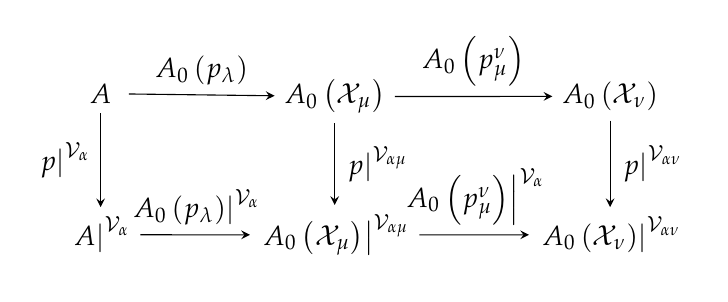
\begin{tikzpicture}
	\matrix (m) [matrix of math nodes,row sep=3em,column sep=4em,minimum width=2em]
	{
		A & A_0\left(\sX_{\mu} \right)  &A_0\left(\sX_{\nu} \right)\\ 
		\left.A\right|^{\sV_\a}	&  \left.A_0\left(\sX_{\mu} \right)\right|^{\sV_{\a   \mu}}  & \left.A_0\left(\sX_{\nu} \right)\right|^{\sV_{ \a  \nu}} \\};
	\path[-stealth]
	(m-1-1) edge node [above] {$A_0\left( p_\la\right)$} (m-1-2)
	(m-1-2) edge node [above] {$A_0\left( p^\nu_\mu\right) $} (m-1-3)
	(m-2-1) edge node [above] {$\left.A_0\left( p_\la\right)\right|^{\sV_\a}$} (m-2-2)
	(m-2-2) edge node [above] {$\left.A_0\left( p^\nu_\mu\right)\right|^{\sV_\a}$} (m-2-3)
	(m-1-1) edge node [left]  {$\left.p\right|^{\sV_\a}$} (m-2-1)
	(m-1-2) edge node [right] {$\left.p\right|^{\sV_{\a\mu}}$} (m-2-2)
	(m-1-3) edge node [right] {$\left.p\right|^{\sV_{\a\nu}}$} (m-2-3);
	\end{tikzpicture}
	\\
	where $\nu > \mu$. Vertical arrows are surjecive *-homomorphisms to factor algebras. Horizontal arrows are injective homomorphisms. Summarize above construction one has the family of operators $\left\{\left.p\right|^{\sV_{\a\la}}\left(a_\la \right)\in \left.A_0\left(\sX_{\la} \right)\right|^{\sV_{   \la}}\cong \K\left(X_{C\left( \sV_{\a\la}\right)} \right) \right\}$. The family  $\left\{a_\la \right\}$ is special it turns out that it satisfies conditions (a)-(c) of the Definition \ref{special_set_defn}. From these conditions it follows that the family $\left\{\left.p\right|^{\sV_{\a\la}}\left(a_\la \right) \right\}$ is coherent (cf. Definition \ref{top_coh_defn}) 
	and taking into account the Theorem \ref{top_coh_thm} it turns out that $\left\{\left.p\right|^{\sV_{\a\la}}\left(a_\la \right) \right\}$ corresponds to the element $\left.\overline{a}\right|^{\overline{   \mathcal V }_\a}\in \K\left(X_{C_0\left(\overline{   \mathcal V } \right) } \right) $. Otherwise $\left.\overline{a}\right|^{\overline{   \mathcal V }_\a}$ can be represented  by an element $\left.\overline{b}\right|^{\overline{   \mathcal V }_\a}\in A_0\left(\overline{   \mathcal X }\right)$, i.e.
	\be\label{ctr_ba_eqn}
	\left.\overline{a}\right|^{\overline{   \mathcal V }_\a}_{\overline{   x}} = \left.\overline{b}\right|^{\overline{   \mathcal V }_\a}_{\overline{   x}}, \quad\forall\overline{   x} \in \overline{   \mathcal V}_\a
	\ee
 There is the dominated by $\left\{{   \mathcal U }_\a\right\}_{\a \in \mathscr A}$ partition of unity
	$$
	1_{C_b\left( {   \mathcal X}\right)} =\sum_{\a \in \mathscr A} f_\a; \quad f_\a \in C_c\left(\sX \right), \quad \supp f_a \subset \sU_{   \a}. 
	$$
If $\la_{\mathrm{min}}\in \La$ be the minimal element, $\overline{a}=\varphi\left(\left\{a_\la \right\}\right)\in B\left( \oplus_{\overline{x}\in\overline{\sX}}\H_{\overline{p}\left(\overline{x} \right)} \right)$ and $a = a_{\overline{   \mathcal V }}\in A$ then for any $\overline x \in\overline{   \mathcal X}$ one has
\be\label{ctr_ineq1_eqn}
\left\| 	\rep_{\overline x} \left(\overline a \right)\right\|  \le \left\| 	\rep_{\overline p\left( \overline x\right] } \left( a \right)\right\|  \quad \forall \overline x \in \overline \sX.
	\ee
	For each $\eps > 0$ there is a compact set $\sV \subset \sX$ such that
\be\label{ctr_ineq2_eqn}
	\left\| \rep_x\left(a\right) \right\|  < \eps \quad \forall  x \in  \sX \setminus\sV.
\ee
Since $\sV$ is compact there is a finite subset $\mathscr A_0\subset \mathscr A$ such that
\be\label{ctr_ineq3_eqn}
\sum_{\a \in \mathscr A_0} f_\a\left(x \right) =1 \quad\forall x \in \sV
\ee	From \eqref{ctr_ineq1_eqn}-\eqref{ctr_ineq3_eqn}  it turns out that
	\be\label{ctr_bae_eqn}
	\left\| \overline a- \sum_{ \a \in \mathscr A_0}f_\a \left.\overline{b}\right|^{\overline{   \mathcal V }_\a}  \right\| < \eps
	\ee
	where $\left.\overline{b}\right|^{\overline{   \mathcal V }_\a}\in A_0\left(\overline{   \mathcal X }\right)$ is a representative of $\left.\overline{a}\right|^{\overline{   \mathcal V }_\a}$ (cf. \eqref{ctr_ba_eqn}). The set $A_0$ is finite, hence from $f_\a \left.\overline{b}\right|^{\overline{   \mathcal V }_\a} \in A_0\left(\overline{   \mathcal X }\right)$ it follows that $\sum_{ \a \in \mathscr A_0}f_\a \left.\overline{b}\right|^{\overline{   \mathcal V }_\a}\in A_0\left(\overline{   \mathcal X }\right)$ and taking into account \eqref{ctr_bae_eqn} one has $ \varphi\left(\left\{a_\la \right\}\right)= \overline a \in A_0\left(\overline{   \mathcal X }\right)$.
\end{proof}
\begin{corollary}\label{ctr_spec_inc_cor}
	If $\overline{A}$ is the disconnected algebraical inverse noncommutative limit of the given by  \eqref{ctr_base_point_eqn} pointed algebraical  finite covering category then one has $\varphi\left(\overline{A} \right) \subset A_0\left(\overline\sX \right)$ 
\end{corollary}
\begin{proof}
	From the Lemma \ref{ctr_spec_inc_lem} it turns out that $\varphi\left(\left\{b_\la \right\} \right) \subset A_0\left(\overline\sX \right)$ for any special family $\left\{b_\la \right\}$. From the Lemma \ref{top_mult_inc_l_lem} it turns out that $A_0\left(\sX_\la \right) \subset M\left(A_0\left(\overline\sX \right) \right)$. It follows that $C^*$-$\varinjlim_{\la \in \La} A_0\left(\sX_\la \right) \subset  M\left(A_0\left(\overline\sX \right) \right)$. Hence one has 
	$$
\widehat{x}\varphi\left(\left\{b_\la \right\} \right)\widehat{y} \subset A_0\left(\overline\sX \right), \quad \forall	\widehat{x}, \widehat{y} \in C^*\text{-}\varinjlim_{\la \in \La} A_0\left(\sX_\la \right),
	$$
i.e. the $\varphi$-image any weakly special element is contained in  $ A_0\left(\overline\sX \right)$. On other hand $\overline{A}$  is a $C^*$-algebra generated by   weakly special element, so one has $\varphi\left(\overline{A} \right) \subset A_0\left(\overline\sX \right)$.	
\end{proof}
\begin{empt}\label{ctr_transitive_empt} From the Lemma \ref{ctr_c0_inc_lem} and the Corollary \ref{ctr_spec_inc_cor}  it follows that disconnected inverse noncommutative limit of $\mathfrak{S}_{A}$ is isomorphic to $A_0\left( \overline{   \mathcal X }\right)$. 
	According to the Definition \ref{main_defn_full_defn} one has
	\be\nonumber
	G\left(\left.A_0\left(\overline \sX\right) \right|A\right)= \varprojlim_{\la \in \La} G\left(\left.A_0\left(\sX_\la\right) \right|A\right)
	\ee
	and taking into account $G\left(\left.A_0\left(\sX_\la\right) \right|A\right) \cong G\left(\left. \sX_\la \right| \sX\right)$ and $G\left(\left.\overline \sX \right| \sX\right)=  \varprojlim_{\la \in \La}  G\left(\left. \sX_\la \right| \sX\right)$ we conclude that
	\be\label{ctr_ag_eqn}
	G\left(\left.A_0\left(\overline \sX\right) \right|A\right)= G\left(\left.\overline \sX~ \right| \sX\right). 
	\ee
	If $\widetilde{\mathcal X} \subset \overline{\mathcal X}$ is a connected component of $ \overline{\mathcal X}$ then the closed ideal $A_0\left(\widetilde{\mathcal X}\right)\subset A_0\left(\overline{\mathcal X}\right)$ is a maximal connected $C^*$-subalgebra of $A_0\left(\overline{\mathcal X}\right)$. If 
	$$
	G \subset 	G\left(\left.A_0\left(\overline \sX\right) \right|A\right)
	$$
	is the maximal among subgroups among subgroups $G'
	\subset 	G\left(\left.A_0\left(\overline \sX\right) \right|A\right)$ such that $G' A_0\left(\widetilde \sX\right) =A_0\left(\widetilde \sX\right)$ then $G$ is the maximal among subgroups among subgroups $G''
	\subset G\left(\left.\overline \sX \right|\sX\right)$ such that $G''\widetilde  \sX = \widetilde \sX$ (cf. \eqref{comm_ag_eqn}), or equivalently
	\be\label{ctr_gt_eqn}
	G =  G\left(\left.\widetilde \sX \right|\sX\right).
	\ee
	If $J\subset	G\left(\left.A_0\left(\overline \sX\right) \right|A\right)$ is a set of representatives of $$	G\left(\left.A_0\left(\overline \sX\right) \right|A\right)/	G\left(\left.A_0\left(\widetilde \sX\right) \right|A\right)$$ then  from the \eqref{top_disconnected_repr_eqn} it follows that
	\begin{equation*}
	\overline{\mathcal X}=  \bigsqcup_{g \in J} g \widetilde{\mathcal X}
	\end{equation*}
	and $A_0\left( \overline{\mathcal X}\right) $ is a $C^*$-norm completion of the direct sum
	\begin{equation}\label{ctr_transitive_eqn}
	\bigoplus _{g \in J}  g A_0\left( \widetilde{\mathcal X} \right) .
	\end{equation}
	
	
\end{empt}




\begin{theorem}\label{ctr_main_thm}

	Let $A$ be a separable $C^*$-algebra with continuous trace and $\sX= \hat A$ is the spectrum of $A$. 	Let	$\mathfrak{S}_{\left(\sX, x_0\right)}= \left\{p_\la:\left( \sX_\la, x^\la_0\right) \to \left( \sX, x_0\right)\right\}_{\la \in \La} \in \mathfrak{FinTop}^{\mathrm{pt}}$ be a pointed topological finite covering category such that for any $\mu > \nu$ there is the unique  pointed  covering $p^\mu_{ \nu}: \left(\sX_{\mu}, x^\mu_0 \right) \to \left(\sX_{\nu}, x^\nu_0 \right)$. 
	 If
\be\nonumber
\begin{split}
	\mathfrak{S}_{A } = \\
	=\left(\left\{A_0\left( p_\la\right) : A  \hookto A_0\left(\sX_\la \right)\right\}, \left\{A_0\left( p_\nu^\mu\right) : A_0\left(\sX_\nu \right) \hookto A_0\left(\sX_\mu \right)\right\}\right)
\end{split}
\ee
is a given by the Lemma  \ref{ctr_base_point_lem} {pointed algebraical  finite covering category} (cf. Definition \ref{comp_pt_defn}).
then following conditions hold:
\begin{enumerate}
	\item [(i)] $\mathfrak{S}_{A}$ is good  and the triple $\left(A, A_0\left(\varprojlim  \mathfrak{S}_{\mathcal X}\right),G\left(\varprojlim  \mathfrak{S}_{\mathcal{X}}~|~ \mathcal X\right)\right)$ is  the  { infinite noncommutative covering} of $\mathfrak{S}_{A}$(cf. Definition \ref{main_defn}).
	\item[(ii)] There are  isomorphisms:
	\begin{itemize}
		\item $\varprojlim  \mathfrak{S}_{A} \approx A_0\left(\varprojlim  \mathfrak{S}_{\mathcal X}\right)$.
		\item $G\left(\varprojlim  \mathfrak{S}_{A}~|~ A\right) \approx G\left(\varprojlim  \mathfrak{S}_{\mathcal{X}}~|~ \mathcal X\right)$.
	\end{itemize}
\end{enumerate}
\end{theorem}

\begin{proof}
	From \ref{ctr_transitive_empt} it follows that the disconnected algebraical inverse noncommutative limit of $	\mathfrak{S}_{A }$  is isomorphic to  $A_0\left(\overline \sX\right)$. According to the Definition \ref{main_defn}  the triple $\left(A, A_0\left(\widetilde\sX\right), G\left(\left.\widetilde \sX~\right| \sX\right) \right)$ should be a   weak infinite noncommutative covering, i.e. it should satisfy to the conditions (a), (b) of the Definition \ref{weak_defn}.
	\begin{enumerate}
		\item [(a)] 	From the Lemma \eqref{top_mult_inc_eqn} it turns out that there is the natural  inclusion  $A_0\left( \sX\right) \subset M\left(A_0\left(\overline \sX\right) \right)$, hence one has 
		$
		C^*$-$\varinjlim_{\la \in \La} A_0\left( \sX_\la\right) \subset  M\left( A_0\left(\overline\sX\right)\right) $.
		\item[(b)] If 
		$$
		G \subset G\left(\left.A_0\left(\overline\sX\right) \right|A\right)
		$$
		is the maximal among subgroups among subgroups $G'
		\subset G\left(\left.A_0\left(\overline\sX\right) \right|A\right)$ such that $G' A_0\left(\widetilde\sX\right) = A_0\left(\widetilde\sX\right)$ then from \eqref{ctr_gt_eqn} it follows that $	G =  G\left(\left.\widetilde M \right|M\right)$.
		Otherwise from the Theorem \ref{ctr_fin_thm} it turns out that $G\left(\left.A_0\left( \sX_\la\right) \right|A\right)\cong G\left(\left.\sX_\la \right|\sX\right)$, and taking into account the surjective homomorphisms $G\left(\left. \widetilde \sX \right|\sX\right)\to  G\left(\left. \sX_\la \right|\sX\right)$ one has the sucjecive homomorphisms   $G\left(\left. A_0\left(\widetilde \sX\right) \right|A\right) \to G\left(\left.A_0\left( \sX_\la\right) \right|A\right)$ for each $\la \in \La$.
	\end{enumerate}
	Now we need check conditions (a) and (b) of the Definition \ref{main_defn}.
	\begin{enumerate}
		\item [(a)] In \ref{ctr_transitive_empt} we already stated that 
		$A_0\left(\widetilde \sX\right)$ is the maximal connected subalgebra of $A_0\left(\overline\sX\right)$.	
		\item[(b)] In \ref{ctr_transitive_empt} we already stated that	 $A_0\left(\overline \sX\right)$ is a $C^*$-norm completion of the direct sum
		$
		\bigoplus _{g \in J} g A_0\left(\widetilde \sX\right)
		$.
	\end{enumerate}
	(ii) Follows from (i) of this lemma.
	
\end{proof}




\begin{lemma}\label{ctr_allows_lem}
	Let $A$ be a $C^*$-algebra with continuous trace, and let $\sX$ be the spectrum of $A$. Suppose that $\sX$ is a connected, locally connected, second-countable Hausdorff space.
	If $\mathfrak{S}_{\left( \mathcal X, x_0\right) } = \left\{\left( \mathcal{X}_\la, x_0^\la\right)  \to \left( \mathcal{X}, x_0\right) \right\}_{\la \in \La} \in \mathfrak{FinTop}^{\mathrm{pt}}$ and
	$$
		\mathfrak{S}^{\mathrm{pt}}_{A } = \\
	=\left\{A_0\left( p_\la\right) : A  \hookto A_0\left(\sX_\la \right)\right\}, \left\{A_0\left( p_\nu^\mu\right) : A_0\left(\sX_\nu \right) \hookto A_0\left(\sX_\mu \right)\right\}
	$$
	is given by the Lemma \ref{ctr_base_point_lem} pointed algebraical  finite covering category then $\mathfrak{S}^{\mathrm{pt}}_{A }$ allows inner product (cf. Definition \ref{inf_hilb_prod_defn}). 
\end{lemma}

\begin{proof}
	The proof is similar to the proof of the Lemma \ref{comm_allows_lem}.
	%	Denote by $G_\la = G\left(\mathcal X_\la~|~\mathcal X \right)$ groups of covering transformations and $\widehat{G} = \varprojlim G_\la$. 
	Denote by $\widetilde{p}:\widetilde{  \mathcal X} \to \mathcal X$, $\widetilde{p}_\la:\widetilde{  \mathcal X} \to \mathcal X_\la$, $p^\la:  \mathcal X_\la \to \mathcal X$, $p^\mu_\la:  \mathcal X_\mu \to \mathcal X_\la$ ($\mu > \la$) the natural covering projections.
	If $\widetilde{\sX}= \varprojlim \mathfrak{S}_{\left(\sX, x_0 \right)}$ then  	from the Theorem \ref{ctr_main_thm} it turns out	
	$$\left(A, A_0\left(\widetilde{\sX}\right),G\left(\widetilde{\sX}~|~ \mathcal X\right)\right)$$ is  the  { infinite noncommutative covering} of $\mathfrak{S}^{\mathrm{pt}}_{A }$ (cf. Definition \ref{main_defn}). 
	 Theorem \ref{ctr_as_field_thm} represented by the following way
	\be\nonumber
	A = C_0\left( \sX, \left\{A_x\right\}_{x \in \sX}, \sF\right)
	\ee
	where the notation \eqref{top_res_eqn} is used.	
If $\mathscr C = \left( \sX, \left\{A_x\right\}_{x \in \sX}, \sF\right)$	From \eqref{top_c0i_ob_eqn} and  the  Definitions \ref{top_cs_funct_b_defn}, \ref{ctr_funct_not_defn}	it turns that
	$$
	A_0\left(\widetilde{\sX}\right)\stackrel{\text{def}}{=}\mathscr C_0\left(\widetilde{\sX}\right)\stackrel{\text{def}}{=} C_0\left(\lift_p\left[\sX, \left\{A_x\right\}, \sF \right] \right)
	$$
	If $\widetilde a \in   C_0\left(\lift_p\left[\sX, \left\{A_x\right\}, \sF \right] \right)
	$  lies in the Pederesen's ideal of $C_0\left(\lift_p\left[\sX, \left\{A_x\right\}, \sF \right] \right)$ then the given by \eqref{top_support_eqn} set $\supp \widetilde a$ is a compact subset of $\widetilde\sX$.
	From the Lemma \ref{top_comp_la_lem} it follows that there is $\la_0 \in \La$ such that for all $\la \ge \la_0$ the restriction $\left.\widetilde{p}_\la\right|_{\supp \overline{a}}$ is injective. From (ii) of the Lemma  \ref{comm_lift_desc_sum_lem} it follows that
	\begin{equation}\nonumber
	\begin{split}
	c_{\la} = \sum_{g \in \ker\left(G\left(\left.\widetilde{\sX}~\right|\sX \right)  \to  G\left( \sX_{\la}~|~\sX \right)\right)} g \left(\widetilde{a}^* \widetilde{b}  \right) = \desc_{\overline{p}_\la}\left( \widetilde{a}\widetilde{b}\right) 
	\end{split}
	\end{equation}
	where notation  $\desc_{\overline{p}_\la}$ means  the descent	(cf. Definition \ref{top_lift_desc_defn}). From the properties of the descent it turns out that $\desc_{\overline{p}_\la}\left( \widetilde{a}\widetilde{b}\right) \in A_0\left( \sX_{\la}\right)$, i.e. $c_\la \in A_0\left( \sX_{\la}\right)$.  Taking into account the Remark \ref{inf_hilb_prod_low_rem} we conclude that  $c_\la \in A_0\left( \sX_{\la}\right)$ for all $\la \in \La$.
\end{proof}




\subsection{Universal noncommutative coverings and  fundamental groups}
\paragraph*{}
Following theorem gives universal approximately finite coverings of commutative $C^*$-algebras. 






\begin{theorem}\label{ctr_uni_lim_thm}
	Let $A$ be a separable $C^*$-algebra with continuous trace, such that the spectrum $\mathcal X$ of 
$A$ is a connected locally connected locally compact second-countable Hausdorff space. If there is   the universal topological covering $\widetilde{p}:\widetilde{\sX}\to \mathcal X$ (cf. Definition \ref{top_uni_cov_defn}) such that $G\left( \left.{\widetilde{\sX}}~\right|\sX\right)$ is residually finite group then the triple 	$$
\left( A ,  A_0\left( \widetilde{   \mathcal X }\right), G\left( \left.{\widetilde{\sX}}~\right|\sX\right) \right)
$$ 
is the universal covering of $A$ (cf. Definition \ref{fg_bas_defn}).
\end{theorem}

\begin{proof}
	Denote by the {(topological)  finite covering category} $\mathfrak{S}_{\sX} = \left\{p_\la : \sX_\la \to \sX\right\}_{\la \in \La}$ (cf. Definition \ref{top_sec_defn}) such that \textit{any} finite-fold transitive covering $\widetilde{\sX}' \to \sX$ belongs to $\mathfrak{S}_{\sX}$. 
	From the Corollary \ref{ctr_functor_cor} it turns out that	there is the {(algebraical)  finite covering category} $\mathfrak{S}_{A} = \left\{\pi_\la : A  \hookto A\left( \sX_\la\right)  \right\}_{\la \in \La}$. From the Theorem \ref{ctr_fin_thm} it follows that any noncommutative finite-fold covering $ A \hookto A'$ belongs to $\mathfrak{S}_{A}$.	
From the Lemma \ref{ctr_base_point_lem} the  pointed a topological finite covering category $\mathfrak{S}_{\left( \sX, \widetilde{p}\left(\widetilde{x}_0 \right)  \right)}  $ induces the {pointed algebraical  finite covering category} $\mathfrak{S}_{A }^{\text{pt}}$ given by \eqref{ctr_base_point_eqn}, i.e.
	\be\nonumber
\begin{split}
	\mathfrak{S}_{A }^{\text{pt}} = \\
\left\{A_0\left( p_\la\right) : A  \hookto A_0\left(\sX_\la \right)\right\}, \left\{A_0\left( p_\nu^\mu\right) : A_0\left(\sX_\nu \right) \hookto A_0\left(\sX_\mu \right)\right\}.
\end{split}
\ee

 From the Theorem  \ref{ctr_fin_thm} it turns out that 	$\left( A,  A\left( \widetilde{   \mathcal X }\right), G\left( \left.{\widetilde{\sX}}~\right|\sX\right) \right)$ is infinite noncommutative covering of $\mathfrak{S}_{A}$ 	(cf. Definition \ref{main_defn}), and taking into account the Definition \ref{fg_bas_defn} one concludes that 	$\left( A,  A\left( \widetilde{   \mathcal X }\right), G\left( \left.{\widetilde{\sX}}~\right|\sX\right) \right)$ is the universal covering of $A$.
\end{proof}
\begin{cor}
		Let $A$ be a separable $C^*$-algebra, such that the spectrum $\mathcal X$ of 	$A$ is is a connected locally connected locally compact second-countable Hausdorff space.
	If $\mathcal X$ is	a locally path connected semilocally 1-connected space, then
	\begin{enumerate}
		\item [(i)] $A$ {has the algebraical universal approximately finite covering}.
		\item[(ii)] Moreover if $\pi_1\left( \sX, x_0\right)$ is residually finite then there is the group isomorphism 
		\be\label{ctr_fg_iso_eqn}
				\pi_1\left( \sX, x_0\right)\cong\pi_1\left( A, \left\{A_0\left(p^\mu_\nu \right)\right\}\right).
			\ee
		 
	\end{enumerate}
\end{cor}
\begin{proof}
	(i) From the Lemmas \ref{top_simply_con_cov_lem} and \ref{top_uni_exist_spa_lem} it turns out that there is the universal covering $\widetilde{\sX} \to \sX$. From the Corollary \ref{top_cov_pi1_cor} it turns out that $\pi_1\left(\sX, x_0 \right)\approx  G\left(\left.\widetilde{\sX}~\right|\sX\right)$, hence $G\left(\left.\widetilde{\sX}~\right|\sX\right)$ is residually finite. From the Theorem \ref{ctr_uni_lim_thm} it follows that $A_0\left(\widetilde{\sX} \right)$ is the universal covering of $A$.\\
	(ii)	 Let  $\widetilde{p}:\widetilde{\sX} \to \sX$ be the universal covering of $\sX$ and let $\widetilde{x}_0\in \widetilde{\sX}$ be such that $\widetilde{p}\left( \widetilde{x}_0 \right) = x_0$. If $\widetilde{p}_\la: \widetilde{\sX} \to \sX_\la$ are natural coverings and $x^\la_0 = \widetilde{p}_\la\left( \widetilde{x}_0\right)$ then there is a pointed topological finite covering category $ \mathfrak{S}_{\left( \sX, \widetilde{p}\left(\widetilde{x}_0 \right) \right)}= \left\{p_\la:\left( \sX_\la, x^\la_0\right) \to \left( \sX, x_0\right)\right\}$. From the Lemma \ref{ctr_base_point_lem} there is the associated to $\mathfrak{S}_{\left( \sX, \widetilde{p}\left(\widetilde{x}_0 \right) \right)}$
	 pointed algebraical finite covering category $\left(\left\{A_0\left( p_\la\right): A  \to A_0\left( \sX_\la\right)\right\}, \left\{A_0\left( p^\mu_\nu\right)  \right\}_{\substack{ \mu, \nu \in \La \\ \mu > \nu}} \right)$. 
	 such that $A_0\left(\widetilde\sX \right)$ is the inverse limit of it (cf. Definition \ref{main_defn}). From \eqref{fg_bas_eqn} it follows that
	 $$
	 \pi_1\left(A , \left\{A_0\left( p^\mu_\nu\right) \right\} \right) = G\left(\left.A_0\left( \widetilde{\sX}\right) ~\right|A\right).
	 $$
	 
Otherwise from the Corollary \ref{top_cov_pi1_cor} it follows that $\pi_1\left( {\mathcal X}, x_0\right)\approx G\left(\left.\widetilde{\sX}~\right|\sX\right)$ and taking into account $G\left(\left.A_0\left( \widetilde{\sX}\right) ~\right|~A \right)\cong G\left(\left. \widetilde{\sX} ~\right| \sX  \right)$ one has
\be\nonumber
				\pi_1\left( \sX, x_0\right)\cong\pi_1\left( A, \left\{A_0\left(p^\mu_\nu \right)\right\}\right).
\ee
	 
	 
\end{proof}









\subsection{Coverings of spectral triples}
\paragraph*{} Let $\left( \Coo\left( M\right) \otimes \A_{\mathrm{fin}}, L^2\left( M, S\right)\otimes \C^N, D\right)$ be a commutative spectral triple, and let $p:\widetilde{M} \to M$ be an infinite regular covering such that  the {covering group} $G\left( {\widetilde{M}}~|~M\right)$ (cf. Definition \ref{cov_proj_cov_grp_defn}) is residually finite (cf. Definition \ref{residually_finite_defn}). One can define the 


From the Lemma \ref{top_res_fin_lem} it it turns out that there is a (topological)  finite covering category $\mathfrak{S} = \left\{p_\la: M_\la \to M\right\}$ (cf. \ref{top_sec_defn}) such that  the {(topological) inverse limit} of $\mathfrak{S}$ is naturally homeomorphic  to $\widetilde{M}$. From the Proposition \ref{comm_cov_mani} it follows that $\widetilde{M}$ and $M_\la$ ($\forall \la \in \La$)  have natural structure of the Riemannian manifolds.  Denote by $\widetilde{S}\stackrel{\mathrm{def}}{=} p^*S$ ans $S_\la \stackrel{\mathrm{def}}{=} p_\la^*S$  (for all $\la \in \La$) the inverse images of the Spin-bundle (cf. \ref{top_vb_sub_sub}). Similarly we can define the inverse images $\widetilde{\slashed D}\stackrel{\mathrm{def}}{=}p^*\slashed D$ and ${\slashed D}_\la\stackrel{\mathrm{def}}{=}p_\la^*\slashed D$ (for all $\la \in \La$). From the Lemma \ref{ctr_t_a_lem} and the Theorem \ref{ctr_main_thm} it turns out that 
$
\mathfrak{S}_{C\left(M\right)\otimes \A_{\mathrm{fin}}}=
\left\{C(M)\otimes \A_{\mathrm{fin}}\hookto C(M_\la)\otimes \A_{\mathrm{fin}}\right\}_{\la \in \La}
$
is a good {(algebraical)  finite covering category}, and  the triple $$\left(C\left( M\right) \otimes \A_{\mathrm{fin}},~ C_0\left( \widetilde{M}\right) \otimes \A_{\mathrm{fin}}, G=G\left( \left.\widetilde{M}~\right|M\right)\right)$$ is an  infinite noncommutative covering   of $\mathfrak{S}_{C\left(M\right)}$. 
Otherwise from the Theorem \ref{ctr_fin_sp_tr_thm} it follows that
\begin{equation}\label{ctr_triple_seq_eqn}
\begin{split}
\mathfrak{S}_{\left(C^{\infty}\left( M\right) \otimes \A_{\mathrm{fin}}, L^2\left( M, S\right)\otimes\C^N , D\right) } =
\\
= \left\{
\left(C^{\infty}\left( M_\la\right)\otimes \A_{\mathrm{fin}} , L^2\left( M_\la, S_\la\right) \otimes \C^N, D_\la\right)
\right\}_{\la \in \La}\in \mathfrak{CohTriple}
\end{split}
\end{equation}
is a coherent set of spectral triples. We would like to proof that the coherent set of spectral triples $\mathfrak{S}_{\left(C^{\infty}\left( M\right) \otimes \A_{\mathrm{fin}}, L^2\left( M, S\right)\otimes\C^N , D\right) }$ is regular and  to calculate  the $\left(C\left(M \right)\otimes \A_{\mathrm{fin}} , C_0\left( \widetilde{M}\right) \otimes \A_{\mathrm{fin}}, G  \right)$-lift of $\left(C^{\infty}\left( M\right) \otimes \A_{\mathrm{fin}}, L^2\left( M, S\right)\otimes\C^N , D\right)$. 
\subsubsection{Induced representation}
\paragraph*{} From the Lemma \ref{ctr_allows_lem} it turns out that we can define given by the Section \ref{inf_ind_repr_subsection} induced representation.
Similarly to the Section \ref{ctr_induced_finite_sec}  consider  a finite family $\left\{ a_\a \in C\left(  M\right) \right\}_{\a \in \mathscr A}$ of positive elements such that
\begin{equation*}
\begin{split}
a_\a\left(M \setminus \mathcal{U}_\a \right) = \{0\},\\
1_{C\left( M\right) }= \sum_{\a \in \mathscr A}a_\a.
\end{split}
\end{equation*} 
Similarly to $\ref{ctr_induced_finite_sec}$ for any $\a \in \mathscr A$ we choose an open subset $\widetilde{ \mathcal U}_\a$ which is mapped homeomorphically onto $\mathcal U_\a$ and define  $\widetilde{a}_\a= \mathfrak{lift}_{\widetilde{ \mathcal U}_\a}\left(a_\a \right)  \in C\left(\widetilde{M} \right)$. Denote by $e_\a = \sqrt{a_\a}$, $\widetilde{e}_\a= \sqrt{\widetilde{a}_\a}$. If $\Ga_c\left( \widetilde{M}, \widetilde{S}\right)$ is the space of compactly supported  sections then  similarly to \ref{ctr_smooth_iso_eqn} there is the $\C$-linear isomorphism
\be\label{ctr_smooth_iso_c_eqn}
\begin{split}
	\varphi:\Ga_c\left(\widetilde{M},\widetilde{S} \right)\otimes \C^N \xrightarrow{\approx}\left(  C_c\left(\widetilde{M} \right)\otimes \A_{\mathrm{fin}} \right)  \otimes_{C\left( M\right)\otimes \A_{\mathrm{fin}}}  \left(  \Ga\left(M,S \right)\otimes \C^N\right) , \\
\widetilde{\xi}=	\sum_{\left(g, \a\right)  \in \mathscr A_{\widetilde{\xi}}} \left( g\left(  \widetilde{e}_\a \otimes 1_{\A_{\mathrm{fin}}}\right) \right)  \left( g\left(  \widetilde{e}_\a \otimes 1_{\A_{\mathrm{fin}}}\right)\right)  \widetilde{\xi}  \mapsto
	\\
	  \sum_{\left(g, \a\right)  \in \mathscr A_{\widetilde{\xi}}}   g\left(  \widetilde{e}_\a \otimes 1_{\A_{\mathrm{fin}}}\right)  \otimes \mathfrak{desc}\left( \left( g\left(  \widetilde{e}_\a \otimes 1_{\A_{\mathrm{fin}}}\right)\right) \widetilde{\xi}\right) 
\end{split}
\ee
where $\mathscr A_{\widetilde{\xi}}\subset G \times \mathscr A$ is a finite subset such that
$$
\sum_{\left(g, \a\right)  \in \mathscr A_{\widetilde{\xi}}} \left( g \left(  \widetilde{e}_\a \otimes 1_{\A_{\mathrm{fin}}}\right)\right)  \left( g \left(  \widetilde{e}_\a \otimes 1_{\A_{\mathrm{fin}}}\right)\right) \widetilde{\xi} =\widetilde{\xi}. 
$$
There are dense with respect to Hilbert norm inclusions 
\be
\begin{split}
	\Ga\left( M, S\right)\otimes\C^N \subset L^2\left({M},{S}, \mu\right)\otimes\C^N= L^2\left({M},{S} \right)\otimes\C^N,\\
	C_c\left(\widetilde{M} \right) \otimes_{C\left(M \right) } \left( L^2\left( M, S\right) \otimes\C^N\right) \subset L^2\left(\widetilde{M},\widetilde{S}, \widetilde{\mu}\right) \otimes \C^N =L^2\left(\widetilde{M},\widetilde{S} \right)\otimes \C^N\\
\end{split}
\ee
where $\mu$ and $\widetilde{\mu}$ are Riemannian measures (cf.  \cite{do_carmo:rg}) on $M$, and $\widetilde{M}$ respectively.  Denote by $G \stackrel{\text{def}}{=}G\left( \left.\widetilde{M}~\right|M\right)$, $\widetilde{\mathscr A} \stackrel{\text{def}}{=} G\times \mathscr A$ and for any $\widetilde{\a} = \left( g, \a\right)$ denote by $\widetilde{a}_{\widetilde{\a}}\stackrel{\text{def}}{=}g \widetilde{a}_\a$, $\widetilde{e}_{\widetilde{\a}}\stackrel{\text{def}}{=}g \widetilde{e}_\a$. For any $\widetilde{a} \in C_c\left( \widetilde{M}\right)$ denote by  $\widetilde{\mathscr A}_{\widetilde a} \subset \widetilde{\mathscr A}$ a finite subset such that  $\widetilde a  = \sum_{\widetilde{\a}\in \widetilde{\mathscr A}_{\widetilde a}}\widetilde{a}_{\widetilde{\a}} \widetilde a$. 
Similarly to \eqref{ctr_matr_inc_eqn} There is the diagonal inclusion of matrix algebras
\be\nonumber
\phi: \A_{\mathrm{fin}}= \bigoplus_{j=1}^{K}\mathbb{M}_{n_{j}}\left( \C\right)\hookto \mathbb{M}_{n_1+...+n_K}\left(\C \right).
\ee  
Let us define following elements
\bean
{\xi}  =\sum_{p=1}^N {\xi}_{p} \otimes \mathfrak{e}_j, ~ {\eta}  = \sum_{p=1}^N \widetilde{\eta}_{p} \otimes \mathfrak{e}_j\in \Ga\left({M},{S} \right)\otimes \C^N;\\
\widetilde{a} = \sum_{\substack{j = 1\\ k=1}}^L\widetilde{a}_{jk}\otimes\mathfrak{e}_{jk},~\widetilde{b} = \sum_{\substack{j = 1\\ k=1}}^L\widetilde{b}_{jk}\otimes\mathfrak{e}_{jk}\in C_c\left( \widetilde{M}\right)\otimes \phi\left( \A_{\mathrm{fin}} \right) 
\eean
where $L = n_1+...+n_K$ and  $\mathfrak{e}_{jk}\in  \mathbb{M}_{n_1+...+n_K}\left(\C \right)$ means the $j,k$-elementary matrix (cf. Definition \ref{elementary_defn}), and $\phi$ is given by \eqref{ctr_matr_inc_eqn}. For any $\widetilde{a} \in C_c\left(\widetilde{M} \right)\otimes\A_{\mathrm{fin}}$ denote by $\widetilde{\mathscr A}_{ \widetilde{a}}\subset \widetilde{\mathscr A}$ a finite set such that  $\widetilde{a} = \sum_{\widetilde{\a}\in \widetilde{\mathscr A}_{ \widetilde{a}}}\left(\widetilde{a}_{\widetilde{\a}} \otimes 1_{\A_{\mathrm{fin}}}\right) \widetilde{a}$.
If $$\widetilde{a} \otimes \xi, \widetilde{b} \otimes \eta \in\left(  C_c\left(\widetilde{M} \right)\otimes\A_{\mathrm{fin}} \right) \otimes_{C\left(M \right) } \Ga\left( M, S\right) \otimes\C^N \subset L^2\left(\widetilde{M},\widetilde{S} \right)\otimes\C^N$$ then one has
\bean
{\xi}  =\sum_{j=1}^N {\xi}_{j} \otimes \mathfrak{e}_j, ~ {\eta}  = \sum_{j=1}^N \widetilde{\eta}_{p} \otimes \mathfrak{e}_j\in \Ga\left({M},{S} \right)\otimes \C^N;\\
\widetilde{a} = \sum_{\substack{j = 1\\ k=1}}^L\widetilde{a}_{jk}\otimes\mathfrak{e}_{jk},~\widetilde{b} = \sum_{\substack{j = 1\\ k=1}}^L\widetilde{b}_{jk}\otimes\mathfrak{e}_{jk}\in C_c\left( \widetilde{M}\right)\otimes \phi\left( \A_{\mathrm{fin}} \right) 
\\
\left\langle \widetilde{a}, \widetilde{b} \right\rangle_{C\left({M}\right)  \otimes \A_{\mathrm{fin}}}= \sum_{\widetilde{\a} \in \widetilde{\mathscr A}_{ \widetilde{a}\widetilde{b}}} \left\langle \widetilde{a}_{\widetilde{\a}}\widetilde{a}, \widetilde{b} \right\rangle_{C\left({M}\right)  \otimes \A_{\mathrm{fin}}} = \sum_{\substack{j = 1\\k =1\\l=1}}^L \sum_{\widetilde{\a} \in \widetilde{\mathscr A}_{ \widetilde{a}\widetilde{b}}} \left\langle \widetilde{a}_{\widetilde{\a}}\widetilde{a}_{lj}, \widetilde{b}_{lk} \right\rangle_{C\left({M}\right)} \otimes \mathfrak{e}_{jk}=\\=
\sum_{\substack{j = 1\\k =1\\l=1}}^n \sum_{\widetilde{\a} \in \widetilde{\mathscr A}_{ \widetilde{a}\widetilde{b}}}\mathfrak{desc} \left(  \widetilde{a}_{\widetilde{\a}}\widetilde{a}^*_{lj} \widetilde{b}_{lk} \right) \otimes \mathfrak{e}_{jk}.
\eean

 If  $\H'=L^2\left({M},{S} \right)$ and ${\H} = L^2\left(\widetilde{M},\widetilde{S} \right) \otimes \C^N$ then  the given by \ref{comp_hilb_eqn}  scalar product $\left(\cdot, \cdot \right)_{\text{ind}}$ on  $\left( C_c\left(\widetilde{M} \right)\otimes \A_{\mathrm{fin}} \right) \otimes_{C\left(M \right)\otimes \A_{\mathrm{fin}}} \left( L^2\left( M, S\right)\otimes \C^N\right)$ satisfies to the following equation
\begin{equation}\label{ctr_ind_inf_l2_eqn}
\begin{split}
\left( \widetilde{a} \otimes \xi ,    \widetilde{b} \otimes \eta\right)_{\text{ind}}= \left(\xi, \left\langle \widetilde{a}, \widetilde{b}\right\rangle_{C\left(\widetilde{M} \right)\otimes \A_{\mathrm{fin}} } \eta \right)_{\H}=
\\
=\sum_{\widetilde{\a}\in \widetilde{\mathscr A}_{ \widetilde{a}\widetilde{b}}}\left(\xi, \left\langle \widetilde{a}_{\widetilde{\a}}\widetilde{a}, \widetilde{b}\right\rangle_{C\left(\widetilde{M} \right)\otimes \A_{\mathrm{fin}} } \eta \right)_{\H}=
\\
= \left(\xi,\left(  \sum_{\substack{j = 1\\k =1\\l=1}}^L \sum_{\widetilde{\a} \in \widetilde{\mathscr A}_{ \widetilde{a}\widetilde{b}}}\mathfrak{desc} \left(  \widetilde{a}_{\widetilde{\a}}\widetilde{a}^*_{lj} \widetilde{b}_{lk} \right) \otimes \mathfrak{e}_{jk}\right)  \eta\right)_{\H}=
\\
=	\left(\sum_{p=1}^{N}   {\xi}_{p} \otimes \mathfrak{e}_p,\left(  \sum_{\substack{j = 1\\k =1\\l=1}}^L\sum_{\widetilde{\a} \in \widetilde{\mathscr A}_{ \widetilde{a}\widetilde{b}}}\mathfrak{desc} \left(  \widetilde{a}_{\widetilde{\a}}\widetilde{a}^*_{lj} \widetilde{b}_{lk} \right) \otimes \mathfrak{e}_{jk}\right)  \left( \sum_{p=1}^{N}  {\eta}_{p} \otimes \mathfrak{e}_p\right) \right)_{\H}=
\\
=\sum_{\widetilde{\a} \in \widetilde{\mathscr A}_{ \widetilde{a}\widetilde{b}}}\sum_{\substack{j = 1\\k =1\\l=1}}^L\left(\xi_j, \mathfrak{desc} \left(  \widetilde{a}_{\widetilde{\a}}\widetilde{a}^*_{lj} \widetilde{b}_{lk} \right) \eta_k\right)_{\H'} =
\\
= \sum_{\widetilde{\a} \in \widetilde{\mathscr A}_{ \widetilde{a}\widetilde{b}}}\sum_{\substack{j = 1\\k =1\\l=1}}^L \int_M \left( \xi_j, \mathfrak{desc} \left(  \widetilde{a}_{\widetilde{\a}}\widetilde{a}^*_{lj} \widetilde{b}_{lk} \right) \eta_k\right)_{x} d\mu=
\\
=\sum_{\widetilde{\a} \in \widetilde{\mathscr A}_{ \widetilde{a}\widetilde{b}}}\sum_{\substack{j = 1\\k =1\\l=1}}^L \int_{\widetilde{M}}
\left( \lift_{\widetilde{\sU}_{\widetilde{\a}}}\left(\widetilde{e}_{\widetilde{\a}}\xi_j \right)_{\widetilde{x}},  \widetilde{a}^*_{lj} \widetilde{b}_{lk} ~\lift_{\widetilde{\sU}_{\widetilde{\a}}}\left(\widetilde{e}_{\widetilde{\a}}\eta_k \right)_{\widetilde{x}}\right)_{\widetilde{x}}d \widetilde{   \mu} =
\\
=\sum_{\substack{j = 1\\k =1\\l=1}}^L \int_{\widetilde{M}}
\left( \widetilde{a}_{lj} \lift_p\left(\xi_l \right)_{\widetilde{x}},   \widetilde{b}_{lk} ~\lift_p\left(\eta_k \right)_{\widetilde{x}}\right)_{\widetilde{x}}d \widetilde{   \mu}
=
\\
= \left( \widetilde{a}~ \lift_p\left(\xi \right),  \widetilde{b} ~\lift_p\left(\eta \right)\right)_{L^2\left(\widetilde{M},\widetilde{S} \right)\otimes\C^N}= \left( \widetilde{a} \otimes \xi ,    \widetilde{b} \otimes \eta\right)_{L^2\left(\widetilde{M},\widetilde{S} \right)\otimes\C^N}. \\
\end{split} 
\end{equation}
The equation \eqref{ctr_ind_inf_l2_eqn} means that $\left(\cdot, \cdot \right)_{\text{ind}}= \left(\cdot, \cdot \right)_{L^2\left(\widetilde{M},\widetilde{S} \right)\otimes\C^N}$, and taking into account the dense inclusion 
$$\left( C_c\left(\widetilde{M} \right)\otimes \A_{\mathrm{fin}}\right)  \otimes_{C\left(M \right)\otimes \A_{\mathrm{fin}}} \left(  \Ga\left( M, S\right)\otimes \C^N\right) \subset L^2\left(\widetilde{M},\widetilde{S} \right)\otimes\C^N$$ 
with respect to the Hilbert norm of $L^2\left(\widetilde{M},\widetilde{S}\right) \otimes \C^N$ one concludes that the space of induced representation coincides with $L^2\left(\widetilde{M},\widetilde{S}\right)\otimes\C^N$. If $\varphi$ is given by \ref{ctr_smooth_iso_c_eqn}, $\widetilde{a} \in C_c\left( \widetilde{M}\right)\otimes \A_{\mathrm{fin}}$ and $\widetilde{\xi}\in \Ga_c\left(\widetilde{M},\widetilde{S} \right)\otimes \C^N$ then following condition holds
\be\label{ctr_inf_act_eqn}
\varphi\left( \widetilde{a}  \widetilde{\xi}\right)=  \sum_{\widetilde{\a} \in \mathscr A_{ \widetilde{a}}} \widetilde{a}\left( \widetilde{e}_\a \otimes 1_{\A_{\mathrm{fin}}} \right) \otimes \mathfrak{desc}\left( \left( \widetilde{e}_\a \otimes 1_{\A_{\mathrm{fin}}} \right) \widetilde{\xi}\right). 
\ee
The left part of \eqref{ctr_inf_act_eqn} complies with the natural action of $C_c\left(\widetilde{M}\right)$ on $ L^2\left(\widetilde{M},\widetilde{S} \right)$,  the right part  is consistent with \eqref{comp_hilb_act_eqn}. Since $C_c\left(\widetilde{M}\right)$ is a dense subalgebra of $C_0\left(\widetilde{M}\right)$ the equation \eqref{ctr_inf_act_eqn} is true for any $\widetilde{a} \in C_0\left( \widetilde{M}\right)$.
Summarize above equations one has the following lemma.
\begin{lemma}\label{ctr_ind1_lem}
	If the representation  $\widetilde{\rho}: C_0\left(\widetilde{M}\right) \to  B\left( \widetilde{   \H}\right)  $ is induced by the pair $$\left(C\left(M \right)\otimes \A_{\mathrm{fin}}\to B\left(  L^2\left(M,S \right)\right)\otimes\C^N ,\left(C\left(M \right)\otimes \A_{\mathrm{fin}} , C_0\left( \widetilde{M}\right) \otimes \A_{\mathrm{fin}}, G\left( \left.\widetilde{M}~\right|M\right) \right)  \right)$$ (cf. Definition \ref{induced_repr_inf_defn}) then following conditions holds
	\begin{enumerate}
		\item[(a)] There is the homomorphism of Hilbert spaces $\widetilde{   \H}\cong L^2\left(\widetilde{M},\widetilde{S} \right)$,
		\item[(b)] The representation $\widetilde{\rho}$ is given by the natural action of $C_0\left(\widetilde{M}\right)$ on $ L^2\left(\widetilde{M},\widetilde{S} \right)$.
	\end{enumerate}
\end{lemma}
\begin{proof}
	(a) Follows from \eqref{ctr_ind_inf_l2_eqn}.\\
	(b) Follows from \eqref{ctr_inf_act_eqn}.
\end{proof}




\subsubsection{Smooth elements}

\paragraph*{}
Consider the coherent set
\begin{equation}\label{ctr_coh_eqn}
\begin{split}
\mathfrak{S}_{\left(C^{\infty}\left( M\right)\otimes \A_{\mathrm{fin}} , L^2\left( M, S\right)\otimes \C^N , D\right) } =\\=
 \left\{ 
\left(C^{\infty}\left( M_\la\right) \otimes \A_{\mathrm{fin}}, L^2\left( M_\la, S_\la\right)\otimes \C^N , D_\la\right)
\right\}_{\la\in \La}\in\mathfrak{CohTriple}
\end{split}
\end{equation}
of spectral triples given by \eqref{ctr_triple_seq_eqn}. 
For any $\la \in \La$ denote by $\widetilde{\pi}_\la:\widetilde{M} \to M_\la$ the natural covering.



\begin{lem}\label{ctr_smooth_lem}
	If $\widetilde{W}^\infty$ is the space of 	$\mathfrak{S}_{\left(C^{\infty}\left( M\right)\otimes \A_{\mathrm{fin}} , L^2\left( M, S\right)\otimes \C^N , D\right) }$-smooth elements (cf. Definition \ref{smooth_el_defn}) then
	$$\widetilde{W}^\infty \subset \Coo_c\left(\widetilde{M} \right)\otimes \A_{\mathrm{fin}}\stackrel{\mathrm{def}}{=} \left( \Coo\left(\widetilde{M} \right) \otimes \A_{\mathrm{fin}} \right) \bigcap \left( C_c\left(\widetilde{M} \right)\otimes \A_{\mathrm{fin}}\right) .$$
\end{lem}
\begin{proof}
	It is shown in \cite{pedersen:mea_c} that Pedersen ideal of $C_0\left(\widetilde{M} \right)$ coincides with $C_c\left(\widetilde{M} \right)$. If follows that $K\left( C_0\left(\widetilde{M}\otimes \A_{\mathrm{fin}} \right)\right) = C_c\left(\widetilde{M} \right)\otimes \A_{\mathrm{fin}}$. Taking into account the condition (a) of the Definition \ref{smooth_el_defn} one has
	\be\nonumber
	\widetilde{W}^\infty \in C_c\left(\widetilde{M} \right)\otimes \A_{\mathrm{fin}}.
	\ee  
	If $\widetilde{a} \in C_c\left(\widetilde{M} \right)\otimes \A_{\mathrm{fin}}$ then application of the inclusion \ref{ctr_matr_inc_eqn}, i.e, 
		\be\nonumber
	\phi: \A_{\mathrm{fin}}= \bigoplus_{j=1}^{K}\mathbb{M}_{n_{j}}\left( \C\right)\hookto \mathbb{M}_{n_1+...+n_K}\left(\C \right).
	\ee 
	gives the following equation
	$$
	\widetilde{a} = \sum_{\substack{j = 1\\k =1}}^L	\widetilde{a}_{jk}\otimes \mathfrak{e}_{jk}
	$$
where $\widetilde{a}_{jk} \in C_c\left(\widetilde{M} \right)$, $L = n_1+...+n_K$ and $\mathfrak{e}_{jk}\in  \mathbb{M}_{L}\left(\C \right)$ means the $j,k$-elementary matrix (cf. Definition \ref{elementary_defn}). The set $\widetilde{\sU}= \bigcup_{\substack{j = 1\\k =1}}^L \supp \widetilde{a}_{jk}$ is compact, hence from the Lemma \ref{top_comp_la_lem} it follows that there is $\mu \in \La$ such that for any $\la \ge \mu$ the restriction $\left.\widetilde{p}_\la\right|_{\widetilde{\sU}}: \widetilde{\sU} \xrightarrow{\approx} \widetilde{p}_\la\left( \widetilde{\sU}\right)$ of the map $\widetilde{p}_\la: \widetilde{M}\to M_\la$ is a homeomorphism. On the other hand if $\widetilde{a} \in \widetilde{W}^\infty$ then from the condition (b) of the Definition \ref{smooth_el_defn} it follows that 
\be\label{ctr_al_eqn}
\begin{split}
a_\la= \sum_{g \in \ker\left( \widehat{G} \to  G_\la\right)}g\widetilde{a}=
\sum_{\substack{j = 1\\k =1}}^L{a}_{jk}\otimes \mathfrak{e}_{jk}
\in \Coo\left(M_\la \right)\otimes\A_{\mathrm{fin}},\\
\text{where } {a}_{jk} \in \Coo\left(M_\la \right), \quad j,k =1,...,L;
\end{split}
\ee
and taking into account the homeomorphism $p_\la|_{\widetilde{\sU}}: \widetilde{\sU} \xrightarrow{\approx} p_\la\left( \widetilde{\sU}\right)$ one has
\begin{equation}\label{ctr_a_eqn}
\begin{split}
a_{jk}\left(\widetilde{   p }_\la \left( \widetilde{x}\right)\right) =\left\{
\begin{array}{c l}
\widetilde{   a}_{jk}\left( \widetilde{x}\right) &\widetilde{x} \in   \supp~ \widetilde{a} ~\&~ \widetilde{   p }_\la \left( \widetilde{x}\right) \in \supp~ a_\la \\
0 &\widetilde{   p }_\la \left( \widetilde{x}\right) \notin \supp~ a_\la 
\end{array}\right.\\
\end{split}
\end{equation}
Comparison of \eqref{ctr_al_eqn} and \eqref{ctr_a_eqn} gives $\widetilde{a}_{jk} \in  \Coo\left(\widetilde{M} \right)$ and $\widetilde{a} \in  \Coo\left(\widetilde{M} \right)$ gives $$\widetilde{a}\in \left( \Coo\left(\widetilde{M} \right) \otimes \A_{\mathrm{fin}} \right) \bigcap \left( C_c\left(\widetilde{M} \right)\otimes \A_{\mathrm{fin}}\right).$$
\end{proof}


\begin{lem}\label{ctr_smooth_inv_lem}
	If $\widetilde{W}^\infty$ is the space of 	$\mathfrak{S}_{\left(C^{\infty}\left( M\right) , L^2\left( M, S\right) ,\slashed D\right) }$-smooth elements (cf. Definition \ref{smooth_el_defn}) then $$\Coo_c\left(\widetilde{M} \right)\otimes \A_{\mathrm{fin}}\subset \widetilde{W}^\infty.$$
\end{lem}
\begin{proof}
	Let $\widetilde{a} \in \Coo_c\left(\widetilde{M} \right)\otimes \A_{\mathrm{fin}}$. From the proof of the Lemma \ref{ctr_smooth_lem} it turns out that there is
	$\mu \in \La$ such that for any $\la \ge \mu$ the equations \eqref{ctr_al_eqn}, \eqref{ctr_a_eqn} hold.	One need check that $\widetilde{a}$ satisfies to (a)-(d) of the Definition \ref{smooth_el_defn}.\\
	(a) Follows from $K\left(C_0\left(\widetilde{M} \right) \otimes \A_{\mathrm{fin}}\right) = C_c\left(\widetilde{M} \right)\otimes \A_{\mathrm{fin}}$.\\
	(b) If $\la \ge \mu$ then the condition follows from  \eqref{ctr_a_eqn}. Otherwise there is $\nu \in \La$ such that $\nu \ge \mu$ and $\nu \ge \la$, so if $$a_\nu=\sum_{g \in \ker\left( \widehat{G} \to  G_\nu\right)}g\widetilde{a}=\sum_{\substack{j = 1\\k =1}}^L{a}_{jk}\otimes \mathfrak{e}_{jk} \text{ where } a_{jk} \in C_c\left( M_\nu\right)$$ then one has
	\begin{equation}\label{ctr_an_eqn}
	\begin{split}
	a_{jk}\left(\widetilde{   p }_\nu \left( \widetilde{x}\right)\right) =\left\{
	\begin{array}{c l}
	\widetilde{   a}_{jk}\left( \widetilde{x}\right) &\widetilde{x} \in   \supp~ \widetilde{a} ~\&~ \widetilde{   p }_\nu \left( \widetilde{x}\right) \in \supp~ a_\nu \\
	0 &\widetilde{   p }_\nu \left( \widetilde{x}\right) \notin \supp~ a_\nu 
	\end{array}\right.\\
%	\text{where } a_{jk} \in C_c\left( M_\nu\right) \text{ are such that } a_\nu=\sum_{g \in \ker\left( \widehat{G} \to  G_\nu\right)}g\widetilde{a}=\sum_{\substack{j = 1\\k =1}}^L{a}_{jk}\otimes \mathfrak{e}_{jk}.
	\end{split}
	\end{equation}
	From \eqref{ctr_an_eqn} it follows that ${a}_{jk}\in \Coo\left( M_\nu\right)$, hence we have $a_\nu \in \Coo\left( M_\nu\right)\otimes \A_{\mathrm{fin}}$.  On the other hand
	\be\label{ctr_nula_eqn}
	a_\la = \sum_{g \in G\left(M_\nu~|~M_\la \right)} g a_\nu
	\ee  
	and since right part of \eqref{ctr_nula_eqn} contains finite number of summands one concludes that $a_\la \in \Coo\left( M_\la\right)\otimes \A_{\mathrm{fin}}$.\\
	(c) Can be proven as well as (b) by application of the equation \eqref{ctr_an_eqn}. \\
	(d) 
	The equation \eqref{comm_strong_conv_eqn} means that any $\widetilde{a} \in \Coo_c\left(\widetilde{M} \right)$ satisfies to the condition (b) the Definition \eqref{smooth_el_defn}. The manifold $M$ is compact, so there is a finite set $\left\{\mathcal U_\a\right\}_{\a \in \mathscr A}$ of open sets such that any $\mathcal U_\a$ is evenly covered by $\widetilde{p}:\widetilde{M} \to M$ and $M = \bigcup_{\a \in \mathscr A} \mathcal U_\a$.  There is a partition of unity 
	\begin{equation}\nonumber
	1_{C\left( M\right) } = \sum_{\a \in \mathscr A} a_\a; \text{ where } a_\a \in \Coo\left( M\right).
	\end{equation}
	For any $\a \in \mathscr A$ we select $\widetilde{\mathcal U}_\a$ such that the natural map $\widetilde{\mathcal U}_\a \xrightarrow{\approx} {\mathcal U}_\a$ is a homeomorphism. Denote by $e_\a = \sqrt{a_\a}$ and let $\widetilde{e}_\a \in \Coo_c\left(\widetilde{M} \right)$ is given by
	\begin{equation*}\label{ctr_smooth_cov_eqn}
	\widetilde{e}_\a\left( \widetilde{x}\right)= \left\{
	\begin{array}{c l}
	e_\a \left(\widetilde{p} \left( \widetilde{x}\right) \right)  & \widetilde{x} \in \widetilde{\mathcal U}_\a\\
	0 & \widetilde{x} \notin \widetilde{\mathcal U}_\a
	\end{array}\right.
	\end{equation*}
	Denote by $\widetilde{  \mathscr A}=  G\left(\widetilde{M}~|~ M\right) \times  \mathscr A$ and for any $\widetilde{\a}=\left( g, \a\right)$ denote by $\widetilde{e}_{\widetilde{\a}}= g \widetilde{e}_\a$. 
For any $\widetilde{a} \in C_c\left(\widetilde{M} \right)\otimes \A_{\mathrm{fin}}$ there is a finite subset $\widetilde{  \mathscr A}_{\widetilde{a} }$ such that
	\be\label{ctr_ta_decomp_eqn}
	\begin{split}
		\widetilde{a}= \sum_{\left( g, \a\right)\in \widetilde{  \mathscr A}_{\widetilde{a} }} 	\widetilde{a}\left(\widetilde{e}_{\left( g, \a\right)} \otimes 1_{\A_{\mathrm{fin}}}\right) \left(\widetilde{e}_{\left( g, \a\right)} \otimes 1_{\A_{\mathrm{fin}}}\right)  =
		\\
		=  \sum_{\left(g, \a \right) \in \widetilde{\mathscr A}} \widetilde{a}_{\left(g, \a \right)}=\sum_{\left(g, \a \right) \in \widetilde{\mathscr A}} \widetilde{\phi}_{\left(g, \a \right)}\widetilde{\psi}_{\left(g, \a \right)},
		 \\ 
		\text{ where }  ~~
		\widetilde{\phi}_{\left(g, \a \right)} = \widetilde{a}\left(\widetilde{e}_{\left( g, \a\right)} \otimes 1_{\A_{\mathrm{fin}}}\right);\quad \widetilde{\psi}_{\left(g, \a \right)} = \widetilde{e}_{\left( g, \a\right)}\otimes 1_{\A_{\mathrm{fin}}};
		\\
	\widetilde{a}_{\left(g, \a \right)}= \widetilde{a}\left(\widetilde{e}_{\left( g, \a\right)} \otimes 1_{\A_{\mathrm{fin}}}\right)^2= \widetilde{\phi}_{\left(g, \a \right)}\widetilde{\psi}_{\left(g, \a \right)}.
	\end{split}
	\ee
	
	
	If $a_\la,a_{\left(g, \a \right)}^\la,\phi_{\left(g, \a \right)}^\la, \psi_{\left(g, \a \right)}^\la \in \Coo\left(M_\la \right)$ are given by 
	\begin{equation*}
	\begin{split}
	a_\la = \sum_{g \in \ker\left(G\left( \left.\widetilde{M}~\right|M\right)\to G\left(\widetilde{M}~|~M_\la \right)  \right)}g \widetilde{a},
	\\a_{\left(g, \a \right)}^\la = \sum_{g \in \ker\left(G\left( \left.\widetilde{M}~\right|M\right)\to G\left(\widetilde{M}~|~M_\la \right)  \right)}g \widetilde{a}_{\left(g, \a \right)},
	\\\\\phi_{\left(g, \a \right)}^\la = \sum_{g \in \ker\left(G\left( \left.\widetilde{M}~\right|M\right)\to G\left(\widetilde{M}~|~M_\la \right)  \right)}g \widetilde{\phi}_{\left(g, \a \right)},
	\\
	\psi_{\left(g, \a \right)}^\la = \sum_{g \in \ker\left(G\left( \left.\widetilde{M}~\right|M\right)\to G\left(\widetilde{M}~|~M_\la \right)  \right)}g \widetilde{\psi}_{\left(g, \a \right)},\\
	\end{split}
	\end{equation*}
	then 
	\begin{equation*}
	\begin{split}
	\left[ D_\la, a_\la\right] =\sum_{\left(g, \a \right) \in \widetilde{\mathscr A}}   \left[ { D}_\la, {a}^\la_{\left(g, \a \right)}\right]=\\=\sum_{\left(g, \a \right) \in \widetilde{\mathscr A}} \left(  \left[ { D}_\la, {\phi}^\la_{\left(g, \a \right)}\right]{\psi^\la}_{\left(g, \a \right)}   + \phi^\la_{\left(g, \a \right)}  \left[ { D}_\la, {\psi}^\la_{\left(g, \a \right)}\right]\right). \end{split}
	\end{equation*}
	Similarly to \ref{ctr_comm_eqn} one has
		\begin{equation}\nonumber
	\begin{split}
	\left[ { D}, a_{\left(g, \a \right)}^\la\left( {e}_{\left( g,\la\right)}\otimes 1_{\A_{\mathrm{fin}}}\right) \right]\left( {e}_{\left( g,\la\right)}\otimes 1_{\A_{\mathrm{fin}}}\right) = \left( {e}_{\left( g,\la\right)}\otimes 1_{\A_{\mathrm{fin}}}\right)\left[ { D},  a_{\left(g, \a \right)}^\la\left( {e}_{\left( g,\la\right)}\otimes 1_{\A_{\mathrm{fin}}}\right) \right],
	\end{split}
	\end{equation}
	or, equivalently $$\left[ { D}_\la, {\phi}^\la_{\left(g, \a \right)}\right]{\psi^\la}_{\left(g, \a \right)}= {\psi^\la}_{\left(g, \a \right)} \left[ { D}_\la, {\phi}^\la_{\left(g, \a \right)}\right],$$
	hence one has
	\begin{equation*}
	\begin{split}
	\left[ D_\la, a_\la\right]=\sum_{\left(g, \a \right) \in \widetilde{\mathscr A}_{\widetilde{a}}} \left( {\psi^\la}_{\left(g, \a \right)} \left[ { D}_\la, {\phi}^\la_{\left(g, \a \right)}\right]  + \phi^\la_{\left(g, \a \right)}  \left[ { D}_\la, {\psi}^\la_{\left(g, \a \right)}\right]\right).
	\end{split}
	\end{equation*}
	From \eqref{ctr_ta_decomp_eqn} it turns out 
	\be\label{ctr_al_bt_supn_eqn}
	\supp ~{\phi}^\la_{\left(g, \a \right)} \subset \widetilde{p}_{n}\left( g \widetilde{\mathcal U}_\a\right) ; ~~~\supp ~{\psi}^\la_{\left(g, \a \right)}\subset \widetilde{p}_{\la}\left(  g\widetilde{\mathcal U}_\a\right) .
	\ee
	From the definition of $\widetilde{\mathcal U}_\a$ it turns out that for any nontrivial $g' \in G\left( M_\la~|~M\right)$ following condition holds
	$$
	\widetilde{p}_{n}\left(  g\widetilde{\mathcal U}_\a\right) \bigcap g' \widetilde{p}_{n}\left(  g\widetilde{\mathcal U}_\a\right)= \emptyset.
	$$ 
	and taking into account \eqref{comm_al_bt_supn_eqn} one has
	\bean
	{\phi}^\la_{\left(g, \a \right)}\left(g' {\psi}^\la_{\left(g, \a \right)} \right) = 0,\\
	{\psi}^\la_{\left(g, \a \right)} \left[ { D}_\la, g'{\phi}^\la_{\left(g, \a \right)}\right] = 0,\\ \phi^\la_{\left(g, \a \right)}  \left[ { D}_\la, g'{\psi}^\la_{\left(g, \a \right)}\right]=0.
	\eean
	If $e \in G\left(M_\la ~|~ M \right)$ is the neutral element of $G\left(M_\la ~|~ M \right)$ then from the above equations it turns out
	\bean
	{\psi}^\la_{\left(g, \a \right)} \left[ { D}_\la, \sum_{g' \in G\left(M_\la ~|~ M \right)} g'{\phi}^\la_{\left(g, \a \right)}\right]=\sum_{g' \in G\left(M_\la ~|~ M \right)}  {\psi}^\la_{\left(g, \a \right)} \left[ { D}_\la, g'{\phi}^\la_{\left(g, \a \right)}\right] = \\ ={\psi}^\la_{\left(g, \a \right)} \left[ { D}_\la, {\phi}^\la_{\left(g, \a \right)}\right]+\sum_{g' \in G\left(M_\la ~|~ M \right)\setminus\{e\}} {\psi}^\la_{\left(g, \a \right)} \left[ { D}_\la, g'{\phi}^\la_{\left(g, \a \right)}\right]=\\=
	{\psi}^\la_{\left(g, \a \right)} \left[ { D}_\la, {\phi}^\la_{\left(g, \a \right)}\right] + 0 = {\psi}^\la_{\left(g, \a \right)} \left[ { D}_\la, {\phi}^\la_{\left(g, \a \right)}\right].
	\eean 
	Similarly one has
	$$
	{\phi}^\la_{\left(g, \a \right)} \left[ { D}_\la, \sum_{g' \in G\left(M_\la ~|~ M \right)} g'{\psi}^\la_{\left(g, \a \right)}\right] ={\phi}^\la_{\left(g, \a \right)} \left[ { D}_\la, {\psi}^\la_{\left(g, \a \right)}\right],
	$$
	or if ${a}_{\left(g, \a \right)}, {\phi}_{\left(g, \a \right)}, {\psi}_{\left(g, \a \right)}$ are given by
	\be\label{ctr_al_bt_sum_eqn}
	\begin{split}
		{a}_{\left(g, \a \right)} = \sum_{g' \in G\left(M_\la ~|~ M \right)} g'{a}^\la_{\left(g, \a \right)}~,\\
		{\phi}_{\left(g, \a \right)} = \sum_{g' \in G\left(M_\la ~|~ M \right)} g'{\phi}^\la_{\left(g, \a \right)}~,\\
		{\psi}_{\left(g, \a \right)} = \sum_{g' \in G\left(M_\la ~|~ M \right)} g'{\psi}^\la_{\left(g, \a \right)}\\
	\end{split}
	\ee
	then
	\bean
	{\psi}^\la_{\left(g, \a \right)} \left[ { D}_\la, {\phi}^\la_{\left(g, \a \right)}\right]=\sum_{g' \in G\left(M_\la ~|~ M \right)}  {\psi}^\la_{\left(g, \a \right)} \left[ { D}_\la, g'{\phi}^\la_{\left(g, \a \right)}\right]={\psi}^\la_{\left(g, \a \right)} \left[ { D}_\la, {\phi}_{\left(g, \a \right)}\right],\\
	{\phi}^\la_{\left(g, \a \right)} \left[ { D}_\la, {\psi}^\la_{\left(g, \a \right)}\right]=\sum_{g' \in G\left(M_\la ~|~ M \right)}  {\phi}^\la_{\left(g, \a \right)} \left[ { D}_\la, g'{\psi}^\la_{\left(g, \a \right)}\right]={\phi}^\la_{\left(g, \a \right)} \left[ { D}_\la, {\psi}_{\left(g, \a \right)}\right].\\
	\eean
	Elements ${\phi}_{\left(g, \a \right)}, ~{\psi}_{\left(g, \a \right)}$ are invariant with respect to  $G\left(M_\la ~|~ M \right)$, one has ${\phi}_{\left(g, \a \right)}, ~{\psi}_{\left(g, \a \right)} \in \Coo\left( M\right)$. Since ${ D}_\la$ is the $\widetilde{   p}_\la$-lift of $ D$ following conditions hold:
	
	\be\label{ctr_nt_o_eqn}
	\begin{split}
		% {\psi}^\la_{\left(g, \a \right)} \left[ { D}_\la, {\phi}^\la_{\left(g, \a \right)}\right] = 
		{\psi}^\la_{\left(g, \a \right)} \left[ { D}_\la, {\phi}^\la_{\left(g, \a \right)}\right] = {\psi}^\la_{\left(g, \a \right)} \otimes \left[ { D}, {\phi}_{\left(g, \a \right)}\right] \in\\\in \left( \Coo\left(M_\la \right)\otimes \A_{\mathrm{fin}}\right) \otimes_{\Coo\left(M \right) \otimes \A_{\mathrm{fin}}} \Om^1_{ D} \end{split}
	\ee
	where $\Om^1_{ D}$ is the {module of differential forms associated} with the spectral triple $$\left(C^{\infty}\left( M\right)\otimes \A_{\mathrm{fin}} , L^2\left( M, S\right)\otimes\C^N , D\right)$$ (cf. Definition \ref{ass_cycle_sec}).  From the strong limit $\lim_{\la\in\La} {\psi}^\la_{\left(g, \a \right)}=\widetilde{\psi}_{\left(g, \a \right)}$ it turns out
	\bean
	\lim_{\la \in \La} 1_{C_b\left(\widetilde{M} \right) }\otimes  {\psi}^\la_{\left(g, \a \right)}  \left[ { D}, {\phi}_{\left(g, \a \right)}\right]= \widetilde{\psi}_{\left(g, \a \right)} \otimes \left[ { D}, {\phi}_{\left(g, \a \right)}\right]
	\eean
	and taking into account $\widetilde{\psi}_{\left(g, \a \right)} \in C_c\left( \widetilde{M}\right)\otimes \A_{\mathrm{fin}}\cong K\left( C_0\left(\widetilde{M} \right) \otimes \A_{\mathrm{fin}}\right)$ one has
\bean
	\lim_{n \to \infty} 1_{C_b\left(\widetilde{M} \right)\otimes \A_{\mathrm{fin}} } \otimes {\psi}^\la_{\left(g, \a \right)}  \left[ { D}, {\phi}_{\left(g, \a \right)}\right]
	=\widetilde{\psi}_{\left(g, \a \right)} \otimes \left[ { D}, {\phi}_{\left(g, \a \right)}\right]\in
	\\
	\in K\left( C_0\left(\widetilde{M}\right)  \otimes \A_{\mathrm{fin}} \right) \otimes_{\Coo\left( M\right)\otimes \A_{\mathrm{fin}}}\Om^1_D.
\eean
	Similarly one can prove
\bean
	\lim_{\la \in \La} 1_{C_b\left(\widetilde{M} \right) \otimes \A_{\mathrm{fin}}} \otimes {\phi}^\la_{\left(g, \a \right)}  \left[ { D}, {\psi}_{\left(g, \a \right)}\right]=\widetilde{\phi}_{\left(g, \a \right)} \otimes \left[ { D}, {\psi}_{\left(g, \a \right)}\right]\in 
	\\
	\in K\left( C_0\left(\widetilde{M} \right)\otimes \A_{\mathrm{fin}} \right) \otimes_{\Coo\left( M\right)\otimes \A_{\mathrm{fin}}}\Om^1_{ D}.
\eean
	Summarize above equation one has
	\be\label{ctr_ad_eqn}
	\begin{split}
		\widetilde{a}^{ D}_{\left(g, \a \right)}=\lim_{\la \in \La} 1_{C_b\left(\widetilde{M}\right) \otimes \A_{\mathrm{fin}} } \otimes \left[ { D}_\la, a^\la_{\left(g, \a \right)}\right]=\\= \lim_{\la\in\La}  \left( {\psi^\la}_{\left(g, \a \right)} \otimes \left[ { D}_\la, {\phi}^\la_{\left(g, \a \right)}\right]  + \phi^\la_{\left(g, \a \right)} \otimes  \left[ { D}_\la, {\psi}^\la_{\left(g, \a \right)}\right]\right)=\\=
		\sum_{\left(g, \a \right) \in \widetilde{\mathscr A}_{\widetilde{a}}} \left( \widetilde{\psi}_{\left(g, \a \right)} \otimes \left[ { D}, {\phi}_{\left(g, \a \right)}\right]  + \widetilde{\phi}_{\left(g, \a \right)} \otimes  \left[ { D}, {\psi}_{\left(g, \a \right)}\right]\right).
	\end{split}
	\ee
	From $\widetilde{\phi}_{\left(g, \a \right)}, ~\widetilde{\psi}_{\left(g, \a \right)}\in K\left( C_0\left(\widetilde{M} \right) \right)$, $~\left[ { D}, {\phi}_{\left(g, \a \right)}\right],\left[ { D}, {\psi}_{\left(g, \a \right)}\right]\in \Om^1_{ D}$ it follows that $\widetilde{a}^{ D}_{\left(g, \a \right)} \in  C_c\left(\widetilde{M} \right) \otimes_{\Coo\left( M\right)}\Om^1_{ D}$.
	Taking into account that $\widetilde{\mathscr A}_{\widetilde{a}}$ is a finite set one concludes that
	\be\label{ctr_adl_eqn}
	\widetilde{a}_{ D}=\lim_{\la\in\La} 1_{C_b\left(\widetilde{M} \right) } \otimes \left[ { D}_\la, a_\la\right]= \sum_{\left( g, \a\right)\in \widetilde{\mathscr A}_{\widetilde{a}}} \widetilde{a}^{ D}_{\left(g, \a \right)} \in K\left( C_0\left(\widetilde{M} \right) \right) \otimes_{\Coo\left( M\right)}\Om^1_{ D}. 
	\ee
\end{proof}

\subsubsection{Lift of Dirac operator}
\paragraph{}

Let us use the notation of the proof of the Lemma \ref{ctr_smooth_inv_lem}. We would like to find the operator $\widetilde{D}$ given by \eqref{a_d_eqn} and \eqref{inf_lift_D_eqn}, i.e.
 \begin{equation}\label{ctr_a_d_eqn}
\widetilde{a}_D = \lim_{\la }1_{M\left(\widetilde{A}\right) } \otimes_{}\left[D_\la, \sum_{g \in J_\la}\widetilde{a}\right] = \sum_{j = 1}^k \widetilde{a}_D^j\otimes \om_j \in K\left(\widetilde{A}\right)\otimes_{\A} \Om^1_D,
\end{equation}
\begin{equation}\label{ctr_inf_lift_D_eqn}
\widetilde{D}\left(\widetilde{a} \otimes \xi \right) \stackrel{\mathrm{def}}{=} \sum_{j = 1}^k \widetilde{a}_D^j\otimes \om_j \left(\xi \right)  +\widetilde{a} \otimes D\xi \in K\left(\widetilde{A}\right) \otimes_A \H,
\end{equation}
From \eqref{ctr_ad_eqn} and \eqref{ctr_adl_eqn} it follows that
\be\label{ctr_adf_eqn}
\widetilde{a}_D  = \sum_{\left( g, \a\right)\in \widetilde{\mathscr A}_{\widetilde{a}}} \widetilde{a}^{ D}_{\left(g, \a \right)}=	\sum_{\left(g, \a \right) \in \widetilde{\mathscr A}_{\widetilde{a}}} \left( \widetilde{\psi}_{\left(g, \a \right)} \otimes \left[ { D}, {\phi}_{\left(g, \a \right)}\right]  + \widetilde{\phi}_{\left(g, \a \right)} \otimes  \left[ { D}, {\psi}_{\left(g, \a \right)}\right]\right)
\ee
For any $\xi \in \Ga^\infty\left(M, S \right)$ one has
$$
\supp \widetilde{\psi}_{\left(g, \a \right)} \otimes \left[ { D}, {\phi}_{\left(g, \a \right)}\right]\xi \subset g   \widetilde{\mathcal U}_\a,
$$
so from \eqref{ctr_comm_eqn} it turns out that

\bean
\widetilde{\psi}_{\left(g, \a \right)} \otimes \left[ { D}, {\phi}_{\left(g, \a \right)}\right]\xi = \mathfrak{lift}_{g\widetilde{\mathcal{U}}}\left( \mathfrak{desc} \left( \widetilde{\psi}_{\left(g, \a \right)} \otimes \left[ { D}, {\phi}_{\left(g, \a \right)}\right]\xi \right)\right) =\\= \mathfrak{lift}_{g\widetilde{\mathcal{U}}}\left({\psi}_{\left(g, \a \right)}  \left[ { D}, {\phi}_{\left(g, \a \right)}\right]\xi \right)=\mathfrak{lift}_{g\widetilde{\mathcal{U}}}  \left( \left[ { D}, {\phi}_{\left(g, \a \right)}\right]{\psi}_{\left(g, \a \right)}\xi \right).
\eean
Similarly one has
\bean
\widetilde{\phi}_{\left(g, \a \right)} \otimes \left[ { D}, {\psi}_{\left(g, \a \right)}\right]\xi= \mathfrak{lift}_{g\widetilde{\mathcal{U}}}\left({\psi}_{\left(g, \a \right)}  \left[ { D}, {\phi}_{\left(g, \a \right)}\right]\xi\right),\\
\widetilde{a}_{\left(g, \a \right)}\otimes  { D}\xi= \mathfrak{lift}_{g\widetilde{\mathcal{U}}}\left(a_{\left(g, \a \right)}{ D}\xi\right) 
\eean
from \eqref{d_defn_eqn},  $\mathfrak{lift}_{\widetilde{\mathcal{U}}_{\widetilde\a}}\left( {\ga}_{\widetilde{\a}}\right) = \widetilde{\ga}_{\widetilde{\a}}$ and $\sum_{\widetilde{\a}\in \widetilde{\mathscr A}}~ \widetilde{\ga}_{\widetilde{\a}} = \widetilde{a}$. From \eqref{ctr_d_hom_eqn} it follows that there is the $\widetilde p$-{inverse image} $\widetilde{p}^{-1} { D}$ of $D$ (cf. Definition \ref{top_smooth_inv_im_defn}).
From \eqref{ctr_ad_eqn} it turns out that
\bean
\widetilde{a}^{ D}_{\left(g, \a \right)}\left(\xi \right)  = \mathfrak{lift}_{g\widetilde{\mathcal{U}}}  \left(\left(  \left[ { D}, {\phi}_{\left(g, \a \right)}\right]{\psi}_{\left(g, \a \right)}+{\phi}_{\left(g, \a \right)}\left[ { D}, {\psi}_{\left(g, \a \right)}\right]\right) \xi\right)=\\= \mathfrak{lift}_{g\widetilde{\mathcal{U}}}  \left(\left[ { D}, {\al}_{\left(g, \a \right)}{\psi}_{\left(g, \a \right)}\right]\xi\right) =  \mathfrak{lift}_{g\widetilde{\mathcal{U}}}  \left(\left[ { D}, {a}_{\left(g, \a \right)}\right]\xi\right) ,\\
\eean
hence one has
\be\label{ctr_pre_d_eqn}
\begin{split}
	\widetilde{a}^{ D}_{\left(g, \a \right)}\left(\xi \right) + \widetilde{a}_{\left(g, \a \right)} \otimes  D \xi = \mathfrak{lift}_{g\widetilde{\mathcal{U}}}  \left(\left( \left[ { D}, {a}_{\left(g, \a \right)}\right]+ {a}_{\left(g, \a \right)}{ D}\right) \xi\right) = \\ = \mathfrak{lift}_{g\widetilde{\mathcal{U}}}  \left({ D} {a}_{\left(g, \a \right)}\xi\right) = \widetilde{p}^{-1} { D} \left( \widetilde{a}_{\left(g, \a \right)}\otimes\xi\right) 
\end{split}
\ee

 From \eqref{ctr_inf_lift_D_eqn}, \eqref{ctr_pre_d_eqn} and $\widetilde{a}  = \sum_{\left(g, \a \right) \in \widetilde{\mathscr A}} \widetilde{a}_{\left(g, \a \right)}$ it turns out
\bean
\widetilde{ D}\left( \widetilde{a}\otimes \xi\right) = \sum_{\left(g, \a \right) \in \widetilde{\mathscr A}} \widetilde{ D}\left( \widetilde{a}_{\left(g, \a \right)} \otimes \xi\right)= \widetilde{p}^{-1} { D}\left( \widetilde{a}\otimes \xi\right). 
\eean
The above equation means that 
\be\label{ctr_inf_d_eqn}
\widetilde{ D}=\widetilde{p}^{-1} { D}.
\ee 

\begin{theorem}
	The given by \ref{ctr_triple_seq_eqn} coherent set
	\begin{equation}\nonumber
\begin{split}
\mathfrak{S}_{\left(C^{\infty}\left( M\right) \otimes \A_{\mathrm{fin}}, L^2\left( M, S\right)\otimes\C^N , D\right) } =
\\
= \left\{
\left(C^{\infty}\left( M_\la\right)\otimes \A_{\mathrm{fin}} , L^2\left( M_\la, S_\la\right) \otimes \C^N, D_\la\right)
\right\}_{\la \in \La}\in \mathfrak{CohTriple}
\end{split}
	\end{equation}
	of spectral triples is good (cf. Definition \ref{smooth_alg_defn}). Moreover if 
	$$
	\mathfrak{S}_{C\left(M\right)}=
	\left\{C(M)\hookto C(M_\la)\right\}_{\la \in \La}\in \mathfrak{FinTop},
	$$ 
	$\widetilde{M} = \varprojlim 	\mathfrak{S}_{C\left(M\right)}$ , $\widetilde{p}: \widetilde{M} \to M$ is the natural covering, $\widetilde{S}= \widetilde{p}^*S$  and $\Coo_0\left(\widetilde{M}\right)$ is the completion of  $\Coo\left(\widetilde{M}\right)  \cap C_c\left(\widetilde{M} \right)$ with respect to given by \eqref{smooth_seminorms_eqn}  seminorms  then the triple $\left(\Coo_0\left(\widetilde{M}\right)\otimes \A_{\mathrm{fin}}, L^2\left(\widetilde{M}, \widetilde{S} \right) \otimes \C^N, \widetilde{p}^{-1} { D}  \right) $ is the {limit} of the coherent set	$\mathfrak{S}_{\left(C^{\infty}\left( M\right) \otimes \A_{\mathrm{fin}}, L^2\left( M, S\right)\otimes\C^N , D\right) }$ (cf. Definition \ref{reg_triple_defn}).
\end{theorem}
\begin{proof}
	The algebra $\left( \Coo\left(\widetilde{M}\right) \otimes \A_{\mathrm{fin}} \right) \cap \left( C_c\left(\widetilde{M} \right)\otimes \A_{\mathrm{fin}}\right) $ is dense in $C_0\left(\widetilde{M} \right)\otimes \A_{\mathrm{fin}}$ with respect to $C^*$-norm, so $\Coo_0\left(\widetilde{M}\right)\otimes \A_{\mathrm{fin}}$ is also dense in $C_0\left(\widetilde{M} \right)\otimes \A_{\mathrm{fin}}$. It turns out that  $\mathfrak{S}_{\left(C^{\infty}\left( M\right) \otimes \A_{\mathrm{fin}}, L^2\left( M, S\right)\otimes\C^N , D\right) }$ is good. From the Definition \ref{reg_triple_defn} and \eqref{ctr_inf_d_eqn} it follows that the triple $\left(\Coo_0\left(\widetilde{M}\right)\otimes \A_{\mathrm{fin}}, L^2\left(\widetilde{M}, \widetilde{S} \right) \otimes \C^N, \widetilde{p}^{-1} { D}\right)$ is the {limit} of the coherent set	$\mathfrak{S}_{\left(C^{\infty}\left( M\right) \otimes \A_{\mathrm{fin}}, L^2\left( M, S\right)\otimes\C^N , D\right) }$.
\end{proof}




\chapter{Finite-fold coverings of  noncommutative tori}\label{nt_chap} 
	\paragraph*{}




\section{Coverings of $C^*$-algebra}
\paragraph{}

The finite-fold coverings of  noncommutative tori are described in \cite{clarisson:phd,schwieger:nt_cov}. Here we would like to prove that these coverings comply with the general theory of noncommutative coverings described in \ref{cov_fin_bas_sec}. 
\begin{empt}\label{nt_ff_inclusion_empt}
Let $C\left(\mathbb{T}^n_{\Theta}\right)$ be a noncommutative torus (cf. Definition \ref{nt_defn}).  Denote by $\left\{U_k\right\}_{k \in \Z^n}\subset C\left(\mathbb{T}^n_{\Theta}\right) $ the set of unitary elements which satisfy to \eqref{nt_unitary_product_eqn}. We would like to construct an inclusion $\pi:C\left(\mathbb{T}^n_{\Theta}\right) \hookto C\left(\mathbb{T}^n_{\widetilde{\Theta}}\right)$ where $C\left(\mathbb{T}^n_{\widetilde{\Theta}}\right)$ is another noncommutative torus. Denote by $\left\{\widetilde{U}_k\right\}_{k \in \Z^n}\subset C\left(\mathbb{T}^n_{\widetilde{\Theta}}\right)$ the set of unitary elements which satisfy to \eqref{nt_unitary_product_eqn}, i.e.
\begin{equation}\label{nt_unitary_productc_eqn}
\widetilde{U}_k \widetilde{U}_p = e^{-\pi ik ~\cdot~ \widetilde{\Theta} p} \widetilde{U}_{k + p}
\end{equation}
We suppose that there is a subgroup $\Ga \in \Z^n$ of maximal rank such that
\be\label{nt_inc_eqn}
\widetilde{U}_k \in \pi\left( C\left(\mathbb{T}^n_{\Theta} \right)\right)  \Leftrightarrow k \in \Ga. %\text{ AND } \exists k' \in \Z^n \quad \widetilde{U}_k = U_{k'}
\ee
Recall that, given a subgroup $\Gamma \subsetneqq \Z^n$ of maximal rank, there is an invertible $n \times n$-matrix $M$ with integer valued entries such that $\Gamma = M \mathbb{Z}^n$. It is proven in \cite{schwieger:nt_cov} that the inclusion $\pi:C\left(\mathbb{T}^n_{\Theta}\right) \hookto C\left(\mathbb{T}^n_{\widetilde{\Theta}}\right)$ exists if and only if the following condition holds
\be\nonumber
\Th \in M^{\text{T}} \widetilde{\Th} M + \mathbb{M}_n\left( \Z\right).
\ee
From $\Ga = \Gamma = M \mathbb{Z}^n$ it turns out than $C\left(\mathbb{T}^n_{\Theta} \right)$ is the  $C^*$-norm completion of the $C^*$-linear span of of unitary elements given by
\be\label{nt_cov_un_eqn}
U_k = \widetilde{U}_{Mk} \in C\left(\mathbb{T}^n_{\Theta} \right); \quad k \in \Z^n
\ee
\end{empt}
\begin{lemma}\label{nt_cov_fin_lem}
	If $C\left(\mathbb{T}^n_{\Theta}\right) \subset C\left(\mathbb{T}^n_{\widetilde{\Theta}}\right)$ is a given by 
\ref{nt_ff_inclusion_empt} inclusion then the group
	\be\label{nt_fin_g_eqn}
G = \left\{ \left. g \in \Aut\left(C\left(\mathbb{T}^n_{\widetilde{\Theta}}\right)\right)~\right| ga = a;~~\forall a \in C\left(\mathbb{T}^n_{\Theta}\right) \right\}
\ee
is finite.
\end{lemma}
\begin{proof}
For any $j = 1,..., n$ denote by
$$
		\widetilde{u}_j \stackrel{\text{def}}{=} \widetilde{U}_{k_j },\quad \text{ where } k_j=\left(0,...,\underbrace{ 1}_{j^{\text{th}}-\text{place}},...,0 \right).
$$
From \eqref{nt_inc_eqn} it turns out that for any $j \in 1,..., n$ there is $n_j \in \N$ such that $\widetilde{U}_{n_jk_j}= \widetilde{u}_j^{n_j}\in C\left(\mathbb{T}^n_{\Theta}\right)$. If $C\left(\mathbb{T}^n_{\Theta}\right)_j \subset C\left(\mathbb{T}^n_{\Theta}\right)$ is a commutative $C^*$-subalgebra generated by $\widetilde{u}_j^{n_j}$ and 
$$
C\left(\mathbb{T}^n_{\widetilde{\Theta}}\right)_j =  \left\{\left.\widetilde{a} \in C\left(\mathbb{T}^n_{\widetilde{\Theta}}\right)~\right|\widetilde{a}a=a\widetilde{a} \quad \forall a \in C\left(\mathbb{T}^n_{\Theta}\right)_j\right\} 
$$
then for any $g \in G$ one has $gC\left(\mathbb{T}^n_{\widetilde{\Theta}}\right)_j\subset C\left(\mathbb{T}^n_{\widetilde{\Theta}}\right)_j$. Otherwise $C\left(\mathbb{T}^n_{\widetilde{\Theta}}\right)_j$ is a commutative $C^*$-algebra generated by $u_j$. If $\widetilde{w}= g\widetilde{u}_j$ then $\widetilde{w}^{n_j} = \widetilde{u}^{n_j}_j$, and since $C\left(\mathbb{T}^n_{\widetilde{\Theta}}\right)_j$ is commutative one has
\be\label{nt_root_eqn}
\widetilde{w}^{n_j}\widetilde{u}^{*n_j}_j= \left(\widetilde{w}\widetilde{u}^*_j \right)^{n_j} = 1.
\ee
From \eqref{nt_root_eqn} it turns out that there is $0 \le m_j < n_j$ such  $\widetilde{w} = e^{\frac{2\pi i m_j}{n_j }}\widetilde{u}^*_j$. Similarly one can prove that there are $n_j$ ($j=1, ..., n$) such that for any $g \in G$ there are $0 \le m_j < n_j$ following condition holds
\be\label{nt_exp_eqn}
g \widetilde{U}_{k} = \exp\left( 2\pi i \left(\frac{m_1}{n_1}+...+ \frac{m_n}{n_n}\right)\right)  \widetilde{U}_{k}; \quad \text{where} \quad k= \left(k_1, ..., k_n \right).
\ee
From \eqref{nt_exp_eqn} it turns out that $\left|G\right|= n_1 \cdot ...\cdot n_n$, i.e. $G$ is finite. 
\end{proof}
\begin{empt}
	For any $x \in \R^{n}$ let us consider a continuous map 
	\bean
	f_x:[0,1] \to \Aut\left(C\left(\mathbb{T}^n_{{\Theta}}\right) \right); \\
	t \mapsto \left(  U_k \mapsto e^{2\pi i k \cdot x}U_k\right).
	\eean
	and there is the $\pi$ lift 	$\widetilde{f}_x:[0,1] \to \Aut\left(C\left(\mathbb{T}^n_{\widetilde{\Theta}}\right) \right)$ of $f_x$ given by
\bean
	\widetilde{f}_x\left(t \right) \widetilde{U}_{k} = e^{2\pi i \frac{k'\cdot x}{n}} \widetilde{U}_{k};\\
	\text{where } n \in \N, k' \in \Z^n \text{ are such that } \widetilde{U}_{k}^n = U_{k'} \in C\left(\mathbb{T}^n_{{\Theta}}\right).
\eean
From the Lemma \ref{nt_cov_fin_lem} and the Corollary \ref{lift_unique_cor} it follows that $\widetilde{f}_x$ is the unique $\pi$-lift of $f_x$. From the Lemma \ref{lift_commutes_lem} it turns out that $\widetilde{f}_x$ commutes with the given by \eqref{nt_fin_g_eqn} group $G$.  There is the continuous action 
\be\label{nt_ract_eqn}
\begin{split}
	\R^n \times C\left(\mathbb{T}^n_\Theta\right) \to C\left(\mathbb{T}^n_\Theta\right),\\
	x \bullet U_{k} = f_x\left(1\right) U_k= e^{2\pi i k\cdot x}U_k; \quad \forall x \in \R^n
\end{split}
\ee
which can be uniquely lifted to the continuous action
\be\label{nt_xact_eqn}
\begin{split}
	\R^n \times C\left(\mathbb{T}^n_{\widetilde{\Theta}}\right) \to C\left(\mathbb{T}^n_{\widetilde{\Theta}}\right),\\
x \bullet	\widetilde{U}_{k}= e^{2\pi i \left(M^{-1} k\right)\cdot x}\widetilde{U}_{k}; \quad \forall x \in \R^n
\end{split}
\ee
Clearly one has
\be\label{nt_ker_eqn}
 x \bullet \widetilde{a} = \widetilde{a};~~ \forall \widetilde{a} \in C\left(\mathbb{T}^n_{\widetilde{\Theta}}\right)\Leftrightarrow x \in \Ga
\ee
\end{empt}
\begin{lemma}\label{nt_fin_cov_gr_lem}
	If $G$ is given by \eqref{nt_fin_g_eqn} then there is the natural group isomorphism $G \cong \Z^n/\Ga$.
\end{lemma}
\begin{proof}
	If $x \in \Z^n$ then clearly $x \bullet a = a$ for any $a \in C\left(\mathbb{T}^n_\Theta\right)$ so there is the natural group homomorphism $\phi: \Z^n \to G$. From \eqref{nt_ker_eqn} it turns out that $\ker \phi = \Ga$, i.e. there is the natural inclusion $\Z^n/\Ga \to G$. From the Lemma \ref{lift_commutes_lem} it turns out that the action of $G$ commutes with the action of $\Z^n/\Ga$ on $C\left(\mathbb{T}^n_{\widetilde{\Theta}}\right)$ it follows that $G$ is the direct product $G = G' \otimes \Z^n/\Ga$. Action of $G$ on $C\left(\mathbb{T}^n_{\widetilde{\Theta}}\right) $ induces the unitary action of $G$ on the Hilbert space $L^2\left(C\left(\mathbb{T}^n_{\widetilde{\Theta}}\right), \widetilde{\tau} \right)$. It  follows that there is the following Hilbert direct sum
\be\label{nt_hilb_big_eqn}
	L^2\left(C\left(\mathbb{T}^n_{\widetilde{\Theta}}\right), \tau\right)  = \oplus_{\la\in \La_{G'}}\H_\la \bigoplus \oplus_{\mu\in \La_{\Z^n/\Ga}}\H_\mu
\ee
	where $\La_{G'}$ (resp. $\La_{\Z^n/\Ga}$) is the set of irreducible representations of $G'$ (resp. $\Z^n/\Ga$), $\H_\la$ (resp. $\H_\mu$) is the Hilbert subspace which corresponds to the representation $\la$ (resp. $\mu$).
The group	$\Z^n/\Ga$ is and commutative group, hence any irreducible representation of $\Z^n/\Ga$ has dimension 1. The moduli space of representations if $\Ga^\vee/\Z^n$ where
\be\label{nt_dual_eqn}
\Ga^\vee = \left\{x \in \Q^n ~|~ x \cdot \Ga \in \Z\right\}= M^{-1}\Z^n
\ee
For any  $\overline{x} \in \Ga^\vee/\Z^n$ the corresponding representation $\psi_{\overline{x}}: {\Z^n/\Ga} \times \C \to \C$  is given by
\be\label{nt_char_r_eqn}
\begin{split}
\psi\left(\overline k, z \right), \quad \chi_{\overline{x}}\left( \overline{k}\right)= e^{2\pi i k x};\\
 \text{ where } z \in \C, \quad k \in \Z^n \text{ and } ~x \in \Ga^\vee \text{ are representatives of  } \\ \overline{k}\in \Z^n/\Ga \text{ and } \overline{x} \in \Ga^\vee/\Z^n.
 \end{split}
\ee
So there is a bijective map   $\varphi_{\Z^n/\Ga}:\Z^n/ \Ga^\vee \xrightarrow{\approx} \La_{\Z^n/\Ga}$. From \eqref{nt_xact_eqn} it turns out that
$$
\overline{k}' \bullet	\widetilde{U}_{k} = \chi_{M^{-1}k}\left( \overline{k}'\right)\widetilde{U}_{k}; \text{ where } k' \text{ is representative of } \overline{k}' \in \Z^n/\Ga,
$$
hence one has
\bean
\C\widetilde{U}_k \in \H_{\varphi_{\Z^n/\Ga}\left( {M^{-1}k}\right) }\subset \bigoplus_{\mu\in \La_{\Z^n/\Ga}}\H_\mu
\eean
The $\C$-linear span of $\left\{\widetilde{U}_k\right\}_{k \in \Z^n}$ is dense in 	$L^2\left(C\left(\mathbb{T}^n_{\widetilde{\Theta}}\right)\right) $, so there is the following Hilbert direct sum
\be\label{nt_hilb_little_eqn}
L^2\left(C\left(\mathbb{T}^n_{\widetilde{\Theta}}\right), \tau\right)  =  \oplus_{\mu\in \La_{\Z^n/\Ga}}\H_\mu
\ee
Comparison of \eqref{nt_hilb_big_eqn} and \eqref{nt_hilb_little_eqn} gives $\oplus_{\la\in \La_{G'}}\H_\la= \{0\}$ it turns out that $G'$ is trivial, hence  $G = \Z^n/\Ga$.
\end{proof}

\begin{thm}\label{nt_fin_thm}
In the above situation the triple $\left( C\left(\T^{n}_{{\Th}} \right), C\left(\T^{n}_{\widetilde{\Th}} \right), \Z^n / \Ga, \pi\right)$ is an unital noncommutative finite-fold  covering. 
\end{thm}
\begin{proof}
Both $C\left(\T^{n}_{{\Th}} \right)$, $C\left(\T^{n}_{\widetilde{\Th}} \right)$ are unital $C^*$-algebras, so from the Definition \ref{fin_uni_defn} one needs check the following conditions:
\begin{enumerate}
	\item[(i)] The quadruple $\left( C\left(\T^{n}_{{\Th}} \right), C\left(\T^{n}_{\widetilde{\Th}} \right), \Z^n / \Ga, \pi\right)$ is a {noncommutative finite-fold  pre-covering}. (cf. Definition \ref{fin_pre_defn}).
	\item[(ii)] $C\left(\T^{n}_{\widetilde{\Th}} \right)$ is a finitely generated $C\left(\T^{n}_{{\Th}} \right)$-module.
\end{enumerate}
(i) One needs check (a), (b)  of the Definition \ref{fin_pre_defn}.
\begin{enumerate}
	\item[(a)] Follows from the Lemma \ref{nt_fin_cov_gr_lem}.
	\item[(b)] Suppose
	$$
	\widetilde a = \sum_{k \in \Z^n} c_k \widetilde U_k \in C\left(\T^{n}_{\widetilde{\Th}} \right)^{\Z^n / \Ga}; \quad c_k \in \C.
	$$
	If there is $k \in \Z^n \setminus \Ga$ such that $c_k \neq 0$ and  $\overline k \in \Z^n / \Ga$ is represented by $k$  then $\overline k \widetilde a \neq \widetilde a$, so one has  $\widetilde a \notin C\left(\T^{n}_{\widetilde{\Th}} \right)^{\Z^n / \Ga}$. From this contradiction we conclude that $c_k \neq 0 \Leftrightarrow k \in \Ga$. It follows that $\widetilde a\in C\left(\T^{n}_{{\Th}} \right)$, hence one has $C\left(\T^{n}_{\widetilde{\Th}} \right)^{\Z^n / \Ga}=C\left(\T^{n}_{{\Th}} \right)$.
\end{enumerate}
(ii) 
Let $\widetilde a   \in C\left(\T^{n}_{\widetilde{\Th}} \right)$ be any element given by
$$
\widetilde a = \sum_{\widetilde x \in \Z^n} \widetilde{c}_{\widetilde x} \widetilde{U}_{\widetilde x}.
$$
Let $M \in \mathbb{M}_n\left(\Z\right)$ be such that $\Ga = M\Z^n$. The group $\Z^n / \Ga \cong \Z^n / M\Z^n$, let $N = \left| \Z^n / \Ga\right|$ and  $\left\lbrace \widetilde x_1,\dots, \widetilde x_N\right\rbrace  \subset  \Z^n$ is a set of representatives of  $\Z^n / \Ga$. If 
$$
b_j = \frac{1}{\left|\Z^n / \Ga\right|}\sum_{g \in \Z^n / \Ga}g \left( \widetilde{a}\widetilde{U}^*_{\widetilde x_j}\right) \in C\left(\T^n_\Th \right)
$$ then from the definition of $C\left(\T^n_\Th \right)$ the series
$$
b_j = \sum_{y \in \Z^n} d^j_y  \widetilde{U}_{My}
$$	
is norm convergent and $d^j_y = \widetilde{c}_{My - \widetilde x_j}$. It turns out that
\be\label{nt_bj_eqn}
b_j \widetilde{U}_{\widetilde x_j}= \sum_{y \in \Z^n} \widetilde{c}_{My +\widetilde x_j} \widetilde{U}_{My+ \widetilde x_j}
\ee
Since $\left\lbrace \widetilde x_1,\dots, \widetilde x_N\right\rbrace  \subset  \Z^n$ is a set of representatives of  $\Z^n / \Ga$ from \eqref{nt_bj_eqn} it follows that
\be\label{nt_bjn_eqn}
\sum_{j = 1}^n b_j \widetilde{U}_{\widetilde x_j} = \sum_{\widetilde x \in \Z^n} \widetilde{c}_{\widetilde x} \widetilde{U}_{\widetilde x} = \widetilde a
\ee
The equation \ref{nt_bjn_eqn} means that $C\left(\T^{n}_{\widetilde{\Th}} \right)$ is a left $C\left(\T^{n}_{{\Th}} \right)$-module generated by the finite set $\left\{\widetilde{U}_{\widetilde x_j}\right\}$.
\end{proof}





%\begin{lemma}
%	In the above situation the  unital noncommutative finite-fold  covering $$\left( C\left(\T^{n}_{{\Th}} \right), C\left(\T^{n}_{\widetilde{\Th}} \right), \Z^n / \Ga\right)$$ have a unique map lifting (cf. Definition \ref{upl_defn}). 
%\end{lemma}
%\begin{proof}
%	The linear span of the generators $\left\{\widetilde{U}_x\right\}\in M^{-1}\Z^n$ is dense in $C\left(\T^{n}_{\widetilde{\Th}} \right)$. For any $x \in M^{-1}\Z^n$ there is $m_x \in \N$ such that $m_xx \in \Z^n$, it follows that $\widetilde{U}_x^{m_x} = u_x \in C\left(\T^{n}_{{\Th}}\right) $. Moreover $u_x$ is unitary, so there is a Borel-measured $\varphi_x$ such that $\widetilde{U}_x = \varphi\left(u_x \right)$. From the Corollary \ref{borel_path_lift_cor} it turns out that $\left( C\left(\T^{n}_{{\Th}} \right), C\left(\T^{n}_{\widetilde{\Th}} \right), \Z^n / \Ga\right)$ has the {unique path lifting}
%\end{proof}

\section{Induced representation}\label{nt_i_sec}
\paragraph*{}

Let us consider an unital noncommutative finite-fold  covering $$\left( C\left(\T^{n}_{{\Th}} \right), C\left(\T^{n}_{\widetilde{\Th}} \right), \Z^n / \Ga, \pi\right)$$ given by the Theorem \ref{nt_fin_thm}. The group	$\Z^n/\Ga$ is and commutative group, hence any irreducible representation of $\Z^n/\Ga$ has dimension 1. From the proof of the Lemma \ref{nt_fin_cov_gr_lem} it follows that the moduli space of the irreducible representations $\Z^n / \Ga$ coincides with $\Ga^\vee \Z^n / \Ga$ and any irreducible representation corresponds to a character the given by \eqref{nt_char_r_eqn} character $\chi_{\overline{x}}: \Z^n / \Ga \to \C$. It is known the orthogonality of characters (cf. \cite{hamermesh:group}), i.e.
\be\label{nt_ort_eqn}
\sum_{g \in \Z^n / \Ga} \overline{\chi}_{\overline x_1}\left( g\right) \chi_{\overline x_1}\left( g\right)= \left\{\begin{array}{c l}
\left|\Z^n / \Ga\right|   & \overline x_1 = \overline x_2 \\
0 & \overline x_1 \neq\overline x_2 .
\end{array}\right.
\ee

Otherwise one has
\bean
%\chi_{\overline {x + l}}= \chi_{\overline {x}}; \quad \forall l \in \Z^n,\\
g \widetilde{U}_k = \chi_{\overline {M^{-1}k}}\left(g \right)  \widetilde{U}_k; \forall g \in \Z^n / \Ga
\eean
and taking into account \eqref{nt_ort_eqn} following condition holds
\be\label{nt_hprod_eqn}
\begin{split}
\left\langle \widetilde{U}_{k_1 }, \widetilde{U}_{k_2} \right\rangle_{C\left(\mathbb{T}^n_{{\Th}}\right)} = \sum_{g \in \Z^n / \Ga } g\left( \widetilde{U}^*_{k_1 }\widetilde{U}_{k_2 }\right)=\\ =\sum_{g \in \Z^n / \Ga }\overline{\chi}_{\overline {M^{-1}k_1}}\left( g\right) \chi_{\overline {M^{-1}k_2}}\left( g\right)\widetilde{U}^*_{k_1 }\widetilde{U}_{k_2 }
= \\
= \left\{\begin{array}{c l}
	\left|\Z^n / \Ga\right| U_{M^{-1}\left(k_2 - k_1 \right) } \in C\left(\T^{n}_{{\Th}} \right)  & k_1 - k_2 \in \Ga \\
	0 & k_1 - k_2 \notin \Ga .
\end{array}\right.
\end{split}
\ee
Let $\rho: C\left(\mathbb{T}^n_{{\Th}}\right) \to B\left( L^2\left(C\left(\mathbb{T}^n_{\Theta}\right), \tau\right)\right)$ be the described in \ref{nt_gns_empt} faithful GNS-representation.
If $\widetilde \rho: C\left(\T^{n}_{\widetilde{\Th}} \right) \to B\left(\widetilde \H \right)$ is the induced by the pair 
$$
\left(\rho, \left( C\left(\T^{n}_{{\Th}} \right), C\left(\T^{n}_{\widetilde{\Th}} \right), \Z^n / \Ga, \pi\right)\right)
$$
representation (cf. Definition \ref{induced_repr_defn}) then $\widetilde \H$ is the Hilbert norm completion of the tensor product $C\left(\T^{n}_{\widetilde{\Th}} \right) \otimes_{C\left(\T^{n}_{{\Th}} \right)} L^2\left(C\left(\mathbb{T}^n_{\Theta}\right), \tau\right)$. Denote by $\left(\cdot, \cdot \right)_{\widetilde \H}$ the scalar product on $\widetilde \H$ given by \eqref{induced_prod_equ}.
If $\xi_{l_1}, \xi_{l_2} \in L^2\left(C\left(\mathbb{T}^n_{\Theta}\right), \tau\right)$ be given by \eqref{nt_char_r_eqn} then from \eqref{induced_prod_equ} one has
\bean
\left(\widetilde{U}_{k_1 } \otimes \xi_{l_1} , \widetilde{U}_{k_1 } \otimes \xi_{l_1} \right)_{\widetilde \H} = \left(\xi_{l_1}, \left\langle \widetilde{U}_{k_1 }, \widetilde{U}_{k_2} \right\rangle_{C\left(\mathbb{T}^n_{{\Th}}\right)}\xi_{l_2} \right)_{L^2\left(C\left(\mathbb{T}^n_{\Theta}\right), \tau\right)} =\\
 \left\{\begin{array}{c l}
	\left|\Z^n / \Ga\right|\left( U_{M^{-1}\left(k_2 - k_1 \right) } \xi_{l_1}, \xi_{l_2} \right)_{L^2\left(C\left(\mathbb{T}^n_{\Theta}\right), \tau\right)}  & k_1 - k_2 \in \Ga \\
	0 & k_1 - k_2 \notin \Ga .
\end{array}\right.
\eean
Otherwise from $U_{M^{-1}\left(k_2 - k_1 \right)}\xi_{l_1} = \xi_{M^{-1}\left(k_2 - k_1 \right) + l_1}$ and \eqref{nt_h_product_eqn} it turns out that
\be\label{nt_hh_product_eqn}
\left(\widetilde{U}_{k_1 } \otimes \xi_{l_1} , \widetilde{U}_{k_1 } \otimes \xi_{l_1} \right)_{\widetilde \H} =
\left\{\begin{array}{c l}
	\left|\Z^n / \Ga\right|  & k_1 + Ml_1 = k_2 + Ml_2  \\
	0 & k_1 + Ml_1 \neq k_2 + Ml_2 .
\end{array}\right.
\ee
Otherwise one has
\be
M l_1 + k_1 = M l_2 + k_2 \Rightarrow \widetilde{U}_{k_1 } \otimes \xi_{l_1} = \widetilde{U}_{k_2 } \otimes \xi_{l_2}
\ee
On the other hand there is the described in \ref{nt_gns_empt} faithful representation
$C\left(\mathbb{T}^n_{\widetilde\Theta}\right)  \to B\left( L^2\left(  C\left(\mathbb{T}^n_{\widetilde\Theta}\right), \widetilde\tau\right)\right) $
such that the Hilbert space $L^2\left(  C\left(\mathbb{T}^n_{\widetilde\Theta}\right), \widetilde\tau \right)\cong \ell^2\left(\Z^n\right)$ has the countable orthogonal basis $\left\{\widetilde \xi_k\right\}_{k \in \Z^n}$ and the action $C\left(\mathbb{T}^n_{\widetilde\Theta}\right) \times L^2\left(  C\left(\mathbb{T}^n_{\widetilde\Theta}\right), \widetilde\tau\right) \to L^2\left(  C\left(\mathbb{T}^n_{\widetilde\Theta}\right), \widetilde\tau\right) $
is given by
\be\label{nt_t_act_eqn}
\widetilde{U}_{k } \widetilde\xi_{l} =  \widetilde\xi_{k + l}
\ee
There is the isomorphism
\be\label{nt_h_iso_eqn}
\begin{split}
\phi_{\widetilde \H} \xrightarrow{\approx}L^2\left(  C\left(\mathbb{T}^n_{\widetilde\Theta}\right), \widetilde\tau\right);\\
	\widetilde{U}_{k } \otimes \xi_{l} \mapsto \sqrt{\left|\Z^n / \Ga\right|}~\widetilde\xi_{k + Ml}.
\end{split}
\ee
From \eqref{nt_hh_product_eqn} it follows that $\phi_{\widetilde \H}$ is an isomorphism of Hilbert spaces, and from \eqref{nt_t_act_eqn} it turns out that $\phi_{\widetilde \H}$ is an isomorphism of Hermitian modules. In result one has the following lemma.

\begin{lemma}
If	$\widetilde \rho: C\left(\T^{n}_{\widetilde{\Th}} \right) \to B\left(\widetilde \H \right)$ is the induced by the pair 
	$$
	\left(\rho, \left( C\left(\T^{n}_{{\Th}} \right), C\left(\T^{n}_{\widetilde{\Th}} \right), \Z^n / \Ga, \pi\right)\right)
	$$ then $\widetilde \rho$ is equivalent to the described  \ref{nt_gns_empt} faithful representation.
\end{lemma}



\section{Lift of Dirac operator} 
\paragraph*{}
The Hilbert space of relevant to spectral triple is $\widetilde{\H}^m= \widetilde{\H}\otimes \C^m$ where $m=2^{[n/2]}$ and $\widetilde{\H}$ is described in \ref{nt_i_sec} and the action of $C\left(\mathbb{T}^n_{\widetilde{\Th}} \right)$ on $\widetilde{\H}$ is given by \eqref{nt_t_act_eqn}. The action of $C\left(\mathbb{T}^n_{\widetilde{\Th}} \right)$ on  $\widetilde{\H}^m$ is diagonal. Let $\Om^1_D$ is the {module of differential forms associated} with the spectral triple  $\left( \A, \H, D\right)$ (cf. Definition \ref{ass_cycle_defn}). We suppose that $\Ga = M\Z^n$ where $M \in \mathbb{M}_n\left(\Z\right)$ is a diagonal matrix
$$
M = \begin{pmatrix} k_1  & \dots & 0 \\
\vdots  & \ddots & \vdots \\
0  & \dots & k_n 
\end{pmatrix}\quad k_1,..., k_n \in \N
$$ 
 Let us consider a map
\bean
\nabla : \Coo\left(\mathbb{T}^n_{\widetilde{\Th}} \right) \to \Coo\left(\mathbb{T}^n_{\widetilde{\Th}} \right) \otimes_{\Coo\left(\mathbb{T}^n_{{\Th}} \right)} \Om^1_D,\\
\widetilde{a} \mapsto \sum_{\mu = 1}^n \frac{\partial a}{\partial x_\mu} \otimes u^*_\mu \left[ D, u_\mu \right]= \sum_{\mu = 1}^n \frac{\partial a}{\partial x_\mu} \otimes \ga^\mu
\eean
where $\ga^\mu$ Clifford (Gamma) matrices in $\mathbb{M}_n(\mathbb{C})$ satisfying the relation
\eqref{nt_gam_eqn}

The map satisfies  to the following equation
\be\label{nt_nabla_u_eqn}
\nabla \widetilde{ U}_{\widetilde{l} = \left(\widetilde{l}_1, \dots, \widetilde{l}_n \right) } = \sum_{\mu = 1}^n\frac{\widetilde{l}_\mu}{k_\mu} \widetilde{ \mathcal U}_{\widetilde{l}} \otimes \ga^\mu.
\ee
If  $U_{l = \left(l_1,\dots,l_n \right) }\in \Coo\left(\mathbb{T}^n_{{\Th}} \right)$, $\widetilde{l}'=\left( l_1k_1,\dots, l_nk_n\right)$, $\widetilde{l}'' = \widetilde{l} + \widetilde{l}'$ then  from \eqref{nt_unitary_product} % and \eqref{nt_cov_eqn} 
it turns out
\bean
\widetilde{  U}_{\widetilde{l}} U_l e^{-\pi i\widetilde{l} ~\cdot~ \widetilde{\Theta} \widetilde{l}'} U_{\widetilde{l}''=\widetilde{l} + \widetilde{l}'}
\eean
and taking into account \eqref{nt_nabla_u_eqn} one has
\bean
\nabla \left( \widetilde{  U}_{\widetilde{l}} U_l\right) = e^{-\pi i\widetilde{l} ~\cdot~ \widetilde{\Theta} \widetilde{l}'}\sum_{\mu = 1}^n\frac{l_\mu k_\mu+\widetilde{l}_\mu}{k_\mu} \widetilde{ \mathcal U}_{\widetilde{l}''} \otimes \ga^\mu= \\=e^{-\pi i\widetilde{l} ~\cdot~ \widetilde{\Theta} \widetilde{l}'}\sum_{\mu = 1}^n\frac{\widetilde{l}_\mu}{k_\mu} \widetilde{ \mathcal U}_{\widetilde{l}''} \otimes \ga^\mu + e^{-\pi i\widetilde{l} ~\cdot~ \widetilde{\Theta} \widetilde{l}'}\sum_{\mu = 1}^nl_\mu \widetilde{ \mathcal U}_{\widetilde{l}''} \otimes \ga^\mu=\\= \sum_{\mu = 1}^n\frac{\widetilde{l}_\mu}{k_\mu} \widetilde{  U}_{\widetilde{l}} U_l \otimes \ga^\mu + \sum_{\mu = 1}^nl_\mu \widetilde{  U}_{\widetilde{l}} U_l \otimes \ga^\mu =\\= \sum_{\mu = 1}^n\frac{\widetilde{l}_\mu}{k_\mu}\left(  \widetilde{  U}_{\widetilde{l}} \otimes \ga^\mu\right)  U_l +  \widetilde{  U}_{\widetilde{l}} \otimes \sum_{\mu = 1}^nl_\mu U_l \otimes \ga^\mu =\\=
\left(\nabla\widetilde{  U}_{\widetilde{l}} \right) U_l + \widetilde{  U}_{\widetilde{l}} \otimes \left[D, U_l \right] = \left(\nabla\widetilde{  U}_{\widetilde{l}} \right) U_l + \widetilde{  U}_{\widetilde{l}} \otimes d U_l.
\eean
where $d U_l$ is given by  \eqref{diff_map_eqn}. Right part of the above equation is a specific case of \eqref{conn_defn}, i.e. elements $\widetilde{  U}_{\widetilde{l}}$ satisfy condition $\eqref{conn_defn}$. Since $\C$-linear span of $\left\{\widetilde{  U}_{\widetilde{l}}\right\} $ (resp. $\left\{{  U}_{{l}}\right\}$ ) is dense in $\Coo\left(\mathbb{T}^n_{\widetilde{\Th}} \right)$ (resp. $\Coo\left(\mathbb{T}^n_{{\Th}} \right)$) the map $\nabla$ is a connection. If $\left( \overline{p}_1, \dots,\overline{p}_n\right) \in \Z_{k_1}\times \dots \times \Z_{k_1}$ then from
$$
\left( \overline{p}_1, \dots,\overline{p}_n\right) \widetilde{ U}_{\widetilde{l}} = e^{2\pi i \frac{p_1l_1}{k_1} }\cdot \dots\cdot  e^{2\pi i \frac{p_nl_n}{k_n} } \widetilde{ U}_{\widetilde{l}}
$$
it turns out 
\bean
\nabla\left( \left( \overline{p}_1, \dots,\overline{p}_n\right) \widetilde{ U}_{\widetilde{l}}\right)  = e^{2\pi i \frac{p_1l_1}{k_1} }\cdot ...\cdot  e^{2\pi i \frac{p_nl_n}{k_n} } \sum_{\mu = 1}^n\frac{\widetilde{l}_\mu}{k_\mu} \widetilde{ \mathcal U}_{\widetilde{l}} \otimes \ga^\mu=\left( \overline{p}_1, \dots,\overline{p}_n\right)\left( \nabla \widetilde{ U}_{\widetilde{l}}\right), 
\eean
i.e. $\nabla$ is $\Z_{k_1}\times \dots \times \Z_{k_1}$-equivariant, i.e it satisfies to \eqref{equiv_conn_eqn}. 
If $\widetilde{\xi}_l = \Psi_{\widetilde{ \Th}}\left( \widetilde{U}_{\widetilde{l}}\right)=  \widetilde{U}_l \otimes 1_{C\left(\mathbb{T}^n_{\Th}\right)}$ then from $\left[D,  1_{C\left(\mathbb{T}^n_{\Th}\right)} \right] = 0$ it turns out that given by \eqref{d_defn_eqn} Dirac operator satisfy to following condition
\bean
\widetilde{D} \left( \widetilde{\xi}_{\widetilde{l}} \otimes x\right) = \nabla\left(\widetilde{U}_{\widetilde{l}} \right) \left( 1_{C\left(\mathbb{T}^n_{\Th}\right)} \otimes x\right) + \widetilde{U}_{\widetilde{l}} D\left(   1_{C\left(\mathbb{T}^n_{\Th}\right)} \otimes x\right)= \\= \sum_{\mu = 1}^n\frac{\widetilde{l}_\mu}{k_\mu} \widetilde{ \xi}_{\widetilde{l}} \otimes \ga^\mu x_\mu ; ~~\forall x =\begin{pmatrix} x_1 \\\dots\\ x_m \end{pmatrix} \in \C^m. 
\eean



\section{Coverings of spectral triples}
\paragraph*{} Let us consider following objects
\begin{itemize}
	\item The spectral triple $\left( C^{\infty}(\mathbb{T}^n_{\Theta}),L^2\left(C\left(\mathbb{T}^n_{\Theta}\right), \tau\right)\otimes\mathbb{C}^{m},D\right) $ given by \eqref{nt_sp_tr_eqn},
	\item An unital noncommutative finite-fold  covering $\left(C\left(\mathbb{T}^n_{\Th}\right), C\left(\mathbb{T}^n_{\widetilde{\Th}}\right),\mathbb{Z}_{k_1}\times...\times\mathbb{Z}_{k_n}\right)$ given by the Theorem \ref{nt_fin_thm}.
\end{itemize}

Summarize above constructions one has the following theorem.

\begin{thm}\label{nt_st_fin_cov_thm}
	The $\left(C\left(\mathbb{T}^n_{\Th}\right), C\left(\mathbb{T}^n_{\widetilde{\Th}}\right),\mathbb{Z}_{k_1}\times...\times\mathbb{Z}_{k_n}\right)$-lift of the spectral triple $$\left( C^{\infty}(\mathbb{T}^n_{\Theta}),L^2\left(C\left(\mathbb{T}^n_{\Theta}\right), \tau\right)\otimes\mathbb{C}^{m},D\right) $$ is the spectral  triple $\left(\Coo\left(\mathbb{T}^n_{\widetilde{\Theta}}\right),  L^2\left( C\left(\mathbb{T}^n_{\widetilde{\Theta}}\right)\right) , \widetilde{ D} \right)$.
\end{thm} 
%Similarly to \eqref{nt_diff_mod_eqn} for any $\widetilde{a} \in \Coo\left(\mathbb{T}^n_{\widetilde{\Th}}\right)$ following condition holds
%\begin{equation}\label{nt_diff_cov_mod_eqn}
%\left[\widetilde{D}, \widetilde{a} \right]  = \sum_{\mu = 1}^n \frac{\partial \widetilde{a}}{\partial x_\mu} u^*_\mu \left[ D, u_\mu \right]
%\end{equation}
%where $u_1, \dots, u_n$ are unitary generators of $\Coo\left(\mathbb{T}^n_{{\Th}}\right)$.

   \chapter{Isospectral deformations and their coverings}\label{isospectral_chap}
\section{Finite-fold coverings}\label{isosectral_fin_cov}
\subsection{Basic construction}
\paragraph{}
Let $M$ be a spin - manifold with the smooth action of $\T^2$. 
 Let $\widetilde{x}_0 \in \widetilde{M}$ and $x_0=\pi\left(\widetilde{x}_0 \right)$. Denote by $\varphi: \R^2 \to \R^2 / \Z^2 = \T^2$ the natural covering. There are two closed paths $\om_1, \om_2: \left[0,1 \right]\to M$ given by
\begin{equation*}
\begin{split}
\om_1\left(t \right) = \varphi\left(t, 0 \right) x_0,~
\om_2\left(t \right) = \varphi\left(0, t \right) x_0.
\end{split}
\end{equation*} 
There are  lifts of these paths, i.e. maps $\widetilde{\om}_1 , \widetilde{\om}_2: \left[0,1 \right] \to\widetilde{M}$ such that
\begin{equation*}
\begin{split}
\widetilde{\om}_1\left(0 \right)= \widetilde{\om}_2\left(0 \right)=\widetilde{x}_0,~ \\
\pi\left( \widetilde{\om}_1\left(t \right)\right)  = \om_1\left(t\right),\\
\pi\left( \widetilde{\om}_2\left(t \right)\right)  = \om_2\left(t\right).
\end{split}
\end{equation*}
Since $\pi$ is a finite-fold covering there are $N_1, N_2 \in \N$ such that if 
$$
\gamma_1\left(t \right) = \varphi\left(N_1t, 0 \right) x_0,~
\gamma_2\left(t \right) = \varphi\left(0, N_2t \right) x_0.
$$
and $\widetilde{\gamma}_1$ (resp. $\widetilde{\gamma}_2$) is the lift of $\gamma_1$ (resp. $\gamma_2$) then both $\widetilde{\gamma}_1$, $\widetilde{\gamma}_2$ are closed. Let us select minimal values of $N_1, N_2$. If $\text{pr}_n: S^1 \to S^1$ is an $n$ listed covering and $\text{pr}_{N_1, N2}$ the covering given by
$$
\widetilde{\T}^2 = S^1 \times S^1 \xrightarrow{\text{pr}_{N_1}\times\text{pr}_{N_2}} \to S^1 \times S^1 = \T^2
$$
then there is the action $\widetilde{\T}^2 \times \widetilde{M} \to  \widetilde{M}$ such that


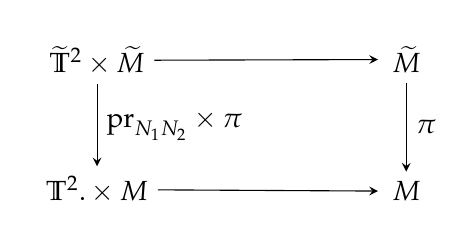
\begin{tikzpicture}
\matrix (m) [matrix of math nodes,row sep=3em,column sep=4em,minimum width=2em]
{
	\widetilde{\T}^2 \times \widetilde{M}  	&  	 & \widetilde{M} \\
	\T^2. \times M 	 & 	 & M   \\};
\path[-stealth]
(m-1-1) edge node [above] {$ \ $} (m-1-3)
(m-1-1) edge node [right] {$\mathrm{pr}_{N_1N_2} \times \pi $} (m-2-1)
(m-1-3) edge node [right] {$\pi$} (m-2-3)
(m-2-1) edge node [above] {$ \ $} (m-2-3);

\end{tikzpicture}


where  $\widetilde{\T}^2 \approx \T^2$.
Let $\widetilde{p} = \left( \widetilde{p}_1, \widetilde{p}_2\right) $ be the generator of the associated with $\widetilde{\T}^2$ two-parameters group $\widetilde{U}\left(s \right) $
so that
\begin{equation*}
\widetilde{U}\left(s \right) = \exp\left( i\left( s_1 \widetilde{p}_1 + s_2 \widetilde{p}_2\right)\right).
\end{equation*}	
The covering $\widetilde{M} \to M$ induces an involutive injective homomorphism
\begin{equation*}
\varphi:\Coo\left(M \right)\to\Coo\left( \widetilde{M} \right).
\end{equation*}


Suppose $M \to M/\T^2$ is submersion, and suppose there is  a weak fibration $\T^2 \to M \to M/\T^2$ (cf. \cite{spanier:at})
There is the exact \textit{homotopy sequence of the weak fibration}
\bean
\dots \to \pi_n\left( \T^2, e_0\right) \xrightarrow{i_{\#}} \pi_n\left( M, e_0\right)  \xrightarrow{p_{\#}} \pi_n\left( M/\T^2, b_0\right) \xrightarrow{\overline\partial} \pi_{n-1}\left( \T^2, e_0\right) \to \dots\\
\dots \to \pi_2\left( M/\T^2, b_0\right) \xrightarrow{\overline\partial} \pi_1\left( \T^2, e_0\right) \xrightarrow{i_{\#}} \pi_1\left( M, e_0\right)  \xrightarrow{p_{\#}} \pi_1\left( M/\T^2, b_0\right) \xrightarrow{\overline\partial} \pi_0\left( \T^2, e_0\right) \to \dots 
\eean
(cf. \cite{spanier:at}) where $\pi_n$ is the $n^{\mathrm{th}}$ homotopical group for any $n\in \N^0$.
If $\pi:\widetilde{M} \to M$ is a finite-fold regular covering then there is the natural surjective homomorphism $
\pi_1\left( M, e_0\right) \to G\left( \left.\widetilde{M}~\right|M\right)$. If $\pi:\widetilde{M} \to M$ induces a covering $\pi:\widetilde{M}/\T^2 \to M / \T^2$  then 
the  homomorphism $
\varphi:\pi_1\left( M, e_0\right) \to G\left( \left.\widetilde{M}~\right|M\right)$ can be included into the following commutative diagram.

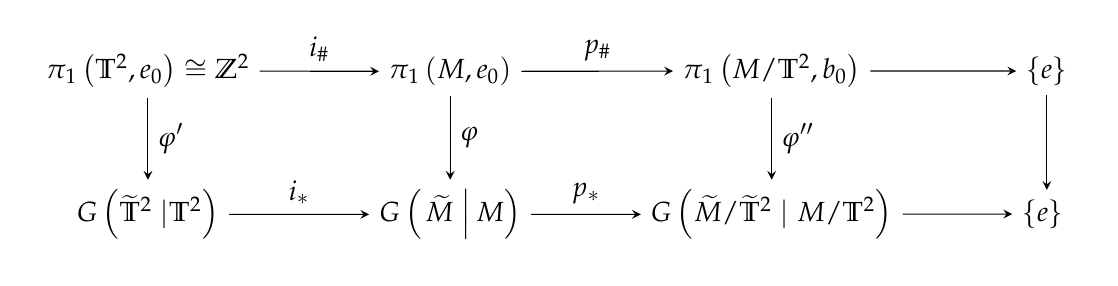
\begin{tikzpicture}
\matrix (m) [matrix of math nodes,row sep=3em,column sep=4em,minimum width=2em]
{
	\pi_1\left(\T^2, e_0 \right)\cong \Z^2 &  \pi_1\left( M, e_0\right) &  \pi_1\left( M/\T^2, b_0\right) &  \{e\} \\
	G\left(\widetilde{\T}^2~|\T^2 \right)  & G\left( \left.\widetilde{M}~\right|M\right) & G\left(\widetilde{M}/\widetilde{\T}^2~|~M/\T^2\right)  & \{e\} \ \\};
\path[-stealth]
(m-1-1)  edge node [right] {$\varphi'$} (m-2-1)
(m-1-2)  edge node [right] {$\varphi$} (m-2-2)
(m-1-3)  edge node [right] {$\varphi''$} (m-2-3)
(m-1-1)  edge node [above] {$i_{\#} $} (m-1-2)
(m-1-2)  edge node [above] {$p_{\#} $} (m-1-3)
(m-2-1)  edge node [above] {$i_*$} (m-2-2)
(m-2-2)  edge node [above] {$p_*$} (m-2-3)
(m-1-3)  edge node [right] {$ $} (m-1-4)
(m-1-4)  edge node [right] {$ $} (m-2-4)
(m-2-3)  edge node [right] {$ $} (m-2-4);
\end{tikzpicture}



Denote by $G \stackrel{\mathrm{def}}{=}G\left( \left.\widetilde{M}~\right|M\right)$, $~G' \stackrel{\mathrm{def}}{=}G\left(\widetilde{\T}^2~|\T^2 \right)$, $~G'' \stackrel{\mathrm{def}}{=}G\left(\widetilde{M}/\widetilde{\T}^2~|~M/\T^2\right)$. From the above construction it turns out that $G' =G\left(\widetilde{\T}^2~|\T^2 \right) = \Z_{N_1} \times \Z_{N_2}$. Otherwise there is an inclusion of Abelian groups $G\left(\widetilde{\T}^2~|\T^2 \right) \subset \widetilde{\T}^2$. The action $\widetilde{\T}^2 \times \widetilde{M} \to  \widetilde{M}$ is free, so the action $G' \times \widetilde{M} \to $ is free, so the natural homomorphism $G' \to G$ is injective, hence there is an exact sequence of groups
\be\label{isospectral_gr_eqn}
\{e\} \to G' \to G \to G'' \to \{e\}.
\ee


Let $\th, \widetilde{\th} \in \R$ be such that
$$
\widetilde{\th}= \frac{\th +  n}{N_1N_2}, \text{ where }n \in \Z.
$$
If $\lambda= e^{2\pi i \th}$, $\widetilde{\lambda}= e^{2\pi i \widetilde{\th}}$ then
$
\lambda = \widetilde{\lambda}^{N_1N_2}.
$
There are isospectral deformations $\Coo\left(M_\th \right), \Coo\left( \widetilde{M}_{\widetilde{\th}} \right)$ and $\C$-linear isomorphisms
$l:\Coo\left(M \right) \to \Coo\left(M_\th \right)$, $\widetilde{l}:\Coo\left( \widetilde{M} \right) \to \Coo\left( \widetilde{M}_{\widetilde{\th}} \right)$.
These isomorphisms and the inclusion $\varphi$ induces the inclusion
\begin{equation*}
\begin{split}
\varphi_\th:\Coo\left(M_\th \right)\to\Coo\left( \widetilde{M}_{\widetilde{\th}} \right),
\\
\varphi_{\widetilde{\th}}\left(\Coo\left(M_\th \right) \right)_{n_1,n_2} \subset \Coo\left( \widetilde{M}_{\widetilde{\th}} \right)_{n_1N_1,~ n_2N_2}.
\end{split}
\end{equation*}
Denote by $G = G\left( \left.\widetilde{M}~\right|M\right)$ the group of covering transformations.   Since $\widetilde{l}$ is a $\C$-linear isomorphism the action of $G$ on $\Coo\left( \widetilde{M} \right)$ induces a $\C$-linear action  $G \times \Coo\left( \widetilde{M}_{ \widetilde{\th}} \right)  \to \Coo\left( \widetilde{M}_{ \widetilde{\th}} \right)$. According to the definition of the action of $\widetilde{\T}^2$ on $\widetilde{M}$ it follows that the action of $G$ commutes with the action of $\widetilde{\T}^2$.
It turns out
$$
g \Coo\left( \widetilde{M} \right)_{n_1,n_2} = \Coo\left( \widetilde{M} \right)_{n_1,n_2}
$$
for any $n_1, n_2 \in \Z$ and $g \in G$.
If $\widetilde{a} \in \Coo\left( \widetilde{M} \right)_{n_1,n_2}$, $\widetilde{b} \in \Coo\left( \widetilde{M} \right)_{n'_1,n'_2}$ then  $g\left( \widetilde{a}\widetilde{b}\right)= \left(g\widetilde{a} \right) \left(g\widetilde{b} \right)\in \Coo\left( \widetilde{M} \right)_{n_1+n'_1,n_2+n'_2} $. One has
\begin{equation*}
	\begin{split}
		\widetilde{l}\left(\widetilde{a}\right)\widetilde{l}\left(\widetilde{b}\right)= \widetilde{\la}^{n'_1n_2}\widetilde{l}\left(\widetilde{a}\widetilde{b}\right), \\
		\widetilde{\la}^{n_2\widetilde{p}_1}l\left( \widetilde{b}\right) = \widetilde{\la}^{n'_1n_2}l\left( \widetilde{b}\right) \widetilde{\la}^{n_2\widetilde{p}_1},\\
		\widetilde{l}\left(g \widetilde{a}\right)\widetilde{l}\left(g \widetilde{b}\right)= g \widetilde{a}\widetilde{\la}^{n_2\widetilde{p}_1}g \widetilde{b}\widetilde{\la}^{n'_2\widetilde{p}_1}= \widetilde{\la}^{n'_1n_2} g\left(\widetilde{a}\widetilde{b} \right) \widetilde{\la}^{\left( n_2+n_2'\right) \widetilde{p}_1}.
	\end{split}
\end{equation*}
On the other hand
\begin{equation*}
	\begin{split}
		g\left( \widetilde{l}\left(\widetilde{a}\right)\widetilde{l}\left(\widetilde{b}\right)\right) = g\left( \widetilde{\la}^{n'_1n_2}\widetilde{l}\left(\widetilde{a}\widetilde{b}\right)\right)= \widetilde{\la}^{n'_1n_2} g\left(\widetilde{a}\widetilde{b} \right) \widetilde{\la}^{\left( n_2+n_2'\right) \widetilde{p}_1}. 
	\end{split}
\end{equation*}
From above equations it turns out
$$
\widetilde{l}\left(g \widetilde{a}\right)\widetilde{l}\left(g \widetilde{b}\right) = g\left( \widetilde{l}\left(\widetilde{a}\right)\widetilde{l}\left(\widetilde{b}\right)\right),
$$
i.e. $g$ corresponds to automorphism of $\Coo\left( \widetilde{M}_{ \widetilde{\th}}\right)$. It turns out that $G$ is the group of automorphisms of $\Coo\left( \widetilde{M}_{ \widetilde{\th}}\right)$. From $\widetilde{a} \in \Coo\left( \widetilde{M}_{ \widetilde{\th}}\right)_{n_1,n_2}$ it follows that $\widetilde{a}^* \in \Coo\left( \widetilde{M}_{ \widetilde{\th}}\right)_{-n_1,-n_2}$. One has
$$
g\left(\left( \widetilde{l}\left(\widetilde{a}\right)\right)^* \right) =  g\left( \widetilde{\la}^{-n_2\widetilde{p_1}}\widetilde{a}^*\right) =
g \left(\widetilde{\la}^{n_1 n_2} \widetilde{a}^*\widetilde{\la}^{-n_2\widetilde{p_1}}\right) = \widetilde{\la}^{n_1 n_2} g\left(\widetilde{l}\left(\widetilde{a}^* \right)  \right). 
$$
On the other hand
$$
\left(g \widetilde{l}\left(\widetilde{a}\right) \right)^*= \left(\left( g \widetilde{a}\right)\widetilde{\la}^{n_2\widetilde{p_1}}  \right)^*=\widetilde{\la}^{-n_2\widetilde{p_1}}\left(ga^* \right) = \widetilde{\la}^{n_1 n_2}\left(ga^* \widetilde{\la}^{-n_2\widetilde{p_1}}\right)= \widetilde{\la}^{n_1 n_2} g\left(\widetilde{l}\left(\widetilde{a}^* \right)  \right),
$$
i.e. $g\left(\left( \widetilde{l}\left(\widetilde{a}\right)\right)^* \right) = \left(g \widetilde{l}\left(\widetilde{a}\right) \right)^*$.
It follows that $g$ corresponds to the involutive automorphism of $\Coo\left( \widetilde{M}_{ \widetilde{\th}}\right)$. Since  $\Coo\left( \widetilde{M}_{ \widetilde{\th}}\right)$ is dense in $C\left( \widetilde{M}_{ \widetilde{\th}}\right)$ there is the unique involutive action $G \times C\left( \widetilde{M}_{ \widetilde{\th}}\right) \to C\left( \widetilde{M}_{ \widetilde{\th}}\right)$.
For any $y_0 \in M/\T^2$ there is a point $x_0 \in M$ mapped onto $y_0$ and a connected submanifold $\mathcal U \subset M$ such that:
\begin{itemize}
	\item $\dim \mathcal U= \dim M-2$,
	\item $\mathcal U$ is transversal to orbits of $\T^2$-action,
	\item The  fibration $\T^2 \to \mathcal U \times \T^2 \to \mathcal U \times \T^2 / \T^2$ is the restriction of the fibration $\T^2 \to M \to M/\T^2$,
	\item The image  $\mathcal V_{y_0} \in M/\T^2$ of $\mathcal U \times \T^2$ in $M/\T^2$ is an open neighborhood of $y_0$,
	\item $\mathcal V_{y_0}$ is evenly covered by  $\widetilde{M}/ \widetilde{\T}^2 \to M / \T^2$.
\end{itemize}
It is clear that
$$
M/\T^2 = \bigcup_{y_0 \in M/\T^2} \mathcal V_{y_0}.
$$
Since $M/\T^2$ is compact there is a finite subset $I \in M/\T^2$ such that
$$
M/\T^2 = \bigcup_{y_0 \in I} \mathcal V_{y_0}.
$$
Above equation will be rewritten as
\be\label{isospectral_p_eqn}
M/\T^2 = \bigcup_{\iota \in I} \mathcal V_{\iota}
\ee
where $\iota$ is just an element of the  finite set $I$ and we denote corresponding transversal submanifold by $\mathcal{U}_\iota$. There is a smooth partition of unity subordinated to \eqref{isospectral_p_eqn}, i.e. there is a set $\left\{a_\iota \in \Coo\left(M /\T^2\right)  \right\}_{\iota \in I}$ of positive elements such that
\be\label{isospectral_part_eqn}
1_{C\left(M /\T^2\right) }= \sum_{\iota \in I} a_\iota~,\\
\ee
\be\nonumber
a_\iota\left(\left( M/\T^2\right)  \setminus \mathcal V_{\iota}\right) = \{0\}.
\ee
Denote by 
\be\label{isospectral_e_eqn}e_\iota \stackrel{\mathrm{def}}{=} \sqrt{a_\iota} \in \Coo\left( M /\T^2\right).
\ee  For any $\iota \in I$ we select an open subset $\widetilde{\mathcal V}_{\iota} \subset \widetilde{M}/\T^2$ which is homeomorphically mapped onto $\mathcal V_{\iota}$.
If $\widetilde{I}= G'' \times  \mathscr A$ then for any $\left(g'', \iota \right) \in \widetilde{I}$ we define
\be\label{isospectral_vgi_eqn}
\begin{split}
	\widetilde{\mathcal V}_{\left(g'', \iota \right)} = g''	\widetilde{\mathcal V}_{\iota}.
\end{split}
\ee
 Similarly we select a transversal submanifold
\be\nonumber%\label{isospectral_u_eqn}
\widetilde{\mathcal U}_{\iota} \subset \widetilde{M}
\ee 
 which is homeomorphially mapped onto $\mathcal U_{\iota}$. For any $\left(g'', \iota \right) \in \widetilde{I}$ we define
 \be\label{isospectral_wgi_eqn}
 \begin{split}
 	\widetilde{\mathcal U}_{\left(g'', \iota \right)} = g	\widetilde{\mathcal U}_{\iota}.
 \end{split}
 \ee
 where $g \in G$ is an arbitrary element mapped to $g''$.
   The set $\mathcal V_{\iota}$ is evenly covered by $\pi'':\widetilde{M}/\widetilde{\T}^2\to M/\T^2$, so one has
\be\label{isostectral_empt_eqn}
g\widetilde{\mathcal V}_{\iota}\bigcap \widetilde{\mathcal V}_{\iota} = \emptyset; \text{ for any nontrivial } g \in G''.
\ee

If $\widetilde{e}_\iota \in \Coo\left(\widetilde M / \widetilde \T^2 \right) $ is given by 
$$
\widetilde{e}_\iota\left(\widetilde{x} \right) = 
\left\{\begin{array}{c l}
e_\iota\left( \pi''\left( \widetilde{x} \right) \right)  & \widetilde{x} \in \widetilde{\mathcal U}_\iota \\
0 & \widetilde{x} \notin \widetilde{\mathcal U}_\iota
\end{array}\right.
$$
then from \eqref{isospectral_part_eqn} and \eqref{isostectral_empt_eqn} it turns out
\begin{equation}
\label{isospectral_partg_eqn}
\begin{split}
1_{C\left(\widetilde M/ \widetilde \T^2 \right) } = \sum_{g \in G''} \sum_{\iota \in I} \widetilde{e}^2_{\iota},\\
\left( g\widetilde{e}_{\iota}\right)\widetilde{e}_{\iota} = 0; \text{ for any nontrivial } g \in G''. 
\end{split}
\end{equation}
If $\widetilde{I}= G'' \times I$ and $\widetilde{e}_{\left(g, \iota\right)} = g \widetilde{e}_{ \iota}$ for any $\left(g, \iota\right)  \in G'' \times I$ then from  \eqref{isospectral_partg_eqn} it turns out
\begin{equation}
\label{isospectral_parti_eqn}
\begin{split}
1_{C\left( \widetilde M / \widetilde \T^2 \right) } =\sum_{\widetilde{\iota} \in \widetilde{I}} \widetilde{e}^2_{\widetilde{\iota}},\\
\left( g\widetilde{e}_{\widetilde{\iota}}\right)\widetilde{e}_{\widetilde{\iota}} = 0; \text{ for any nontrivial } g \in G'',\\
1_{C\left( \widetilde M / \widetilde \T^2 \right) } =  \sum_{\widetilde{\iota} \in \widetilde{I}} \widetilde{e}_{\widetilde{\iota}}\left\rangle \right\langle\widetilde{e}_{\widetilde{\iota}}~.
\end{split}
\end{equation}
It is known that $C\left(\T^2 \right)$ is an universal commutative $C^*$-algebra generated by two unitary elements $u, v$, i.e. there are following relations
\be\label{isospectral_gen_eqn}
\begin{split}
uu^*=u^*u=vv^*=v^*v= 1_{C\left(\T^2 \right)},\\
uv = vu, ~u^*v = vu^*,~uv^*= v^*u, ~ u^*v^*=v^*u^*.
\end{split}
\ee
If $J = I \times \Z \times \Z$ then for any $\left({\iota}, j, k \right) \in J$ there is an element ${f}'_{\left({\iota}, j, k \right)} \in \Coo\left( {\mathcal U}_{{\iota}} \times {\T}^2\right) $ given by
\be\label{isospectral_f's_eqn}
{f}'_{\left({\iota}, j, k \right)} = {e}_{{\iota}} {u}^j{
	v}^k
\ee
where ${e}_{{\iota}}\in \Coo\left( {M}/ {\T}^2\right)$ is regarded as element of $\Coo\left( {M}\right)$.  
Let $p: {M} \to {M} / {\T}^2$.
Denote by ${f}_{\left({\iota}, j, k \right)}\in \Coo\left({M} \right)$ an element given by
\be\label{isospectral_fs_eqn}
\begin{split}
{f}_{\left({\iota}, j, k \right)}\left( {x}\right) =
\left\{\begin{array}{c l}
	{f}'_{\left({\iota}, j, k \right)}\left( {x}\right) & p\left({x} \right)  \in {\mathcal V}_{{\iota}} \\
	0 & p\left( {x}\right)  \notin {\mathcal V}_{{\iota}} 
\end{array}\right.,\\
\text{where the right part of the above equation  assumes the inclusion } \mathcal U_{{\iota}} \times {\T}^2 \hookto M.
\end{split}
\ee 
If we denote by $\widetilde{u}, \widetilde{v} \in U\left( C\left( \widetilde{\T^2} \right) \right)$ unitary generators of $C\left( \widetilde{\T^2} \right)$ then the covering $\pi':\widetilde{\T^2} \to \T^2$ corresponds to a *-homomorphism $C\left(\T^2 \right) \to  C\left( \widetilde{\T^2}\right)$ given by
\bean
u \mapsto \widetilde{u}^{N_1},\\
v \mapsto \widetilde{v}^{N_2}.
\eean
There is the natural action of $G\left( \widetilde{\T}^2~|~{\T^2}\right)\cong \Z_{N_1} \times \Z_{N_2}$ on $C\left(\T^2 \right)$ given by
\be\label{isospectral_uv_eqn}
\begin{split}
\left(\overline{k}_1, \overline{k}_2 \right) \widetilde{u} = e^{\frac{2\pi i k_1}{N_1}}\widetilde{u},\\
\left(\overline{k}_1, \overline{k}_2 \right) \widetilde{v} = e^{\frac{2\pi i k_2}{N_1}}\widetilde{v}
\end{split}
\ee
where $\left(\overline{k}_1, \overline{k}_2 \right) \in \Z_{N_1} \times \Z_{N_2}$. 
If we consider $C\left( \widetilde{\T}^2\right)_{C\left( {\T^2}\right)}$ as a right Hilbert module which corresponds to a finite-fold noncommutative covering then one has
\be\label{isospectral_tor_eqn}
\begin{split}
\left\langle \widetilde{u}^{j'} \widetilde{v}^{k'}, \widetilde{u}^{j''} \widetilde{v}^{k''}  \right\rangle_{C\left( \widetilde{\T^2}\right)} = N_1N_2\delta_{j'j''} \delta_{k'k''}1_{C\left( {\T^2}\right)},\\
1_{C\left( \widetilde{\T^2}\right)}= \frac{1}{N_1N_2}\sum_{\substack{j = 0\\ k = 0}}^{\substack{j = N_1\\ k = N_2}} \widetilde{u}^{j} \widetilde{v}^{k}\left\rangle \right\langle \widetilde{u}^{j} \widetilde{v}^{k}.
\end{split}
\ee
If $\widetilde{J} = \widetilde{I} \times \left\{0, \dots, N_1-1\right\} \times \left\{0, \dots, N_2-1\right\}$ then for any $\left(\widetilde{\iota}, j, k \right) \in \widetilde{J}$ there is an element $\widetilde{f}'_{\left(\widetilde{\iota}, j, k \right)} \in \Coo\left( \widetilde{\mathcal U}_{\widetilde{\iota}} \times \widetilde{\T}^2\right) $ given by
\be\label{isospectral_f'_eqn}
\widetilde{f}'_{\left(\widetilde{\iota}, j, k \right)} = \widetilde{e}_{\widetilde{\iota}} \widetilde{u}^j\widetilde{
v}^k
\ee
where $\widetilde{e}_{\widetilde{\iota}}\in \Coo\left( \widetilde{M}/ \widetilde{\T}^2\right)$ is regarded as element of $\Coo\left( \widetilde{M}\right)$.  
Let $p: \widetilde{M} \to \widetilde{M} / \widetilde{\T}^2$.
Denote by $\widetilde{f}_{\left(\widetilde{\iota}, j, k \right)}\in \Coo\left(\widetilde{M} \right)$ an element given by
\be\label{isospectral_f_eqn}
\begin{split}
\widetilde{f}_{\left(\widetilde{\iota}, j, k \right)}\left( \widetilde{x}\right) =
\left\{\begin{array}{c l}
	\widetilde{f}'_{\left(\widetilde{\iota}, j, k \right)}\left( \widetilde{x}\right) & p\left(\widetilde{x} \right)  \in \widetilde{\mathcal V}_{\widetilde{\iota}} \\
	0 & p\left( \widetilde{x}\right)  \notin \widetilde{\mathcal V}_{\widetilde{\iota}} .
\end{array}\right.\\
\text{where right the part of the above equation assumes the inclusion }  \widetilde{\mathcal U}_{ \widetilde{\iota}} \times  \widetilde{\T}^2 \hookto  \widetilde{M}.
\end{split}
\ee 
Any element $\widetilde{e}_{\widetilde{\iota}} \in C\left(\widetilde{M}/\widetilde{   \T}^2 \right)$ is regarded as element of $C\left(\widetilde{M}\right)$. From $\widetilde{e}_{\widetilde{\iota}} \in \Coo\left(\widetilde{M}\right)_{0,0}$ it turns out $\widetilde{l}\left(\widetilde{e}_{\widetilde{\iota}} \right)  = \widetilde{e}_{\widetilde{\iota}}$,  $~~\left\langle \widetilde{l}\left( \widetilde{e}_{\widetilde{\iota}'}\right) , \widetilde{l}\left( \widetilde{e}_{\widetilde{\iota}''}\right)  \right\rangle_{C\left( \widetilde{M}_{ \widetilde{\th}}\right) } = \left\langle  \widetilde{e}_{\widetilde{\iota}'} ,  \widetilde{e}_{\widetilde{\iota}''}  \right\rangle_{C\left( \widetilde{M}\right) } $.

From \eqref{isospectral_parti_eqn}-\eqref{isospectral_f_eqn} it follows that
\be\label{isospectral_undec_eqn}
1_{C\left(\widetilde{M} \right) }= \frac{1}{N_1N_2}\sum_{\widetilde{\iota} \in \widetilde{I}} \sum_{\substack{j = 0\\ k = 0}}^{\substack{j = N_1-1\\ k = N_2-1}} \widetilde{f}_{\left(\widetilde{\iota}, j, k \right)}\left\rangle \right\langle \widetilde{f}_{\left(\widetilde{\iota}, j, k \right)},
\ee
\be\nonumber%\label{isospectral_fprod_eqn}
\left\langle \widetilde{f}_{\left(\widetilde{\iota}', j', k' \right)}, \widetilde{f}_{\left(\widetilde{\iota}'', j'', k'' \right)} \right\rangle_{C\left( \widetilde{M}\right) } = \frac{1}{N_1N_2} \delta_{j'j''}\delta_{k'k''}\left\langle \widetilde{e}_{\widetilde{\iota}'}, \widetilde{e}_{\widetilde{\iota}''} \right\rangle_{C\left( \widetilde{M}\right) }\in \Coo\left(M \right),
\ee
\be\label{isospectral_fprodl_eqn}
\left\langle \widetilde{l}\left( \widetilde{f}_{\left(\widetilde{\iota}', j', k' \right)}\right) , \widetilde{l}\left( \widetilde{f}_{\left(\widetilde{\iota}'', j'', k'' \right)}\right)  \right\rangle_{C\left( \widetilde{M}_{\widetilde{   \th}}\right) } =\frac{1}{N_1N_2} \delta_{j'j''}\delta_{k'k''}\left\langle \widetilde{e}_{\widetilde{\iota}'}, \widetilde{e}_{\widetilde{\iota}''} \right\rangle_{C\left( \widetilde{M}_{\widetilde{   \th}}\right) }\in  \Coo\left(M_\th \right).
\ee
From the \eqref{isospectral_undec_eqn} it turns out that $C\left(\widetilde{M} \right)$  is a right $C\left(M \right)$ module generated by  finite set of elements $\widetilde{f}_{\left(\widetilde{\iota}, j, k \right)}$ where $\left(\widetilde{\iota}, j, k \right) \in \widetilde{J}$, i.e. any $\widetilde{a} \in C\left(\widetilde{M} \right)$ can be represented as
\be\label{isospectral_wa_eqn}
\widetilde{a} = \sum_{\widetilde{\iota} \in \widetilde{I}} \sum_{\substack{j = 0\\ k = 0}}^{\substack{j = N_1-1\\ k = N_2-1}} \widetilde{f}_{\left(\widetilde{\iota}, j, k \right)} a_{\left(\widetilde{\iota}, j, k \right)}; \text{ where } a_{\left(\widetilde{\iota}, j, k \right)} \in C\left( M\right). 
\ee
Moreover if $\widetilde{a} \in \Coo\left(\widetilde{M} \right)$ then one can select $a_{\left(\widetilde{\iota}, j, k \right)} \in \Coo\left(M \right)$. However any $a_{\left(\widetilde{\iota}, j, k \right)} \in \Coo\left(M \right)$ can be uniquely
written as a doubly infinite
norm convergent sum of homogeneous elements,
\begin{equation*}
a_{\left(\widetilde{\iota}, j, k \right)} = \sum_{n_1,n_2} \, \widehat{T}_{n_1,n_2} \, ,
\end{equation*}

with $\widehat{T}_{n_1,n_2}$ of bidegree $(n_1,n_2)$ and where the sequence
of norms $||
\widehat{T}_{n_1,n_2} ||$ is of
rapid decay in $(n_1,n_2)$. One has
\bea\label{isospectral_sec_eqn}
\widetilde{l}\left(\widetilde{f}_{\left(\widetilde{\iota}, j, k \right)} a_{\left(\widetilde{\iota}, j, k \right)}\right) = \sum_{n_1, n_2}  \widetilde{f}_{\left(\widetilde{\iota}, j, k \right)} \widehat{T}_{n_1,n_2} \widetilde{\lambda}^{\left( N_2n_2+j \right) \widetilde{p}_1}= \sum_{n_1, n_2} \widetilde{f}_{\left(\widetilde{\iota}, j, k \right)} \widetilde{\lambda}^{j \widetilde{p}_1}  \widetilde{\lambda}^{kN_1n_1}\widehat{T}_{n_1,n_2} \widetilde{\lambda}^{N_2n_2 \widetilde{p}_1} 
\eea
%\bea\label{isospectral_sect_eqn}
%\widetilde{l}\left(\widetilde{f}_{\left(\widetilde{\iota}, j, k \right)} a_{\left(\widetilde{\iota}, j, k \right)}\right) = \sum_{n_1, n_2}  \widetilde{f}_{\left(\widetilde{\iota}, j, k \right)} \widehat{T}_{n_1,n_2} \widetilde{\lambda}^{\left( N_2n_2+j \right) \widetilde{p}_1}= \sum_{n_1, n_2} \widetilde{f}_{\left(\widetilde{\iota}, j, k \right)} \widetilde{\lambda}^{j \widetilde{p}_1}  \widetilde{\lambda}^{kN_1n_1}\widehat{T}_{n_1,n_2} \widetilde{\lambda}^{N_2n_2 \widetilde{p}_1} 
%\eea

the sequence
of norms $||
\widetilde{\lambda}^{kN_2n_2}\widehat{T}_{n_1,n_2} ||=||
\widehat{T}_{n_1,n_2} ||$ is of
rapid decay in $(n_1,n_2)$ it follows that
\begin{equation}\label{isospectral_a_eqn}
a'_{\left(\widetilde{\iota}, j, k \right)} = \sum_{n_1,n_2} \, \widetilde{\lambda}^{kN_1n_1} \widehat{T}_{n_1,n_2} \in \Coo\left(M \right) 
\end{equation}
From \eqref{isospectral_wa_eqn} - \eqref{isospectral_a_eqn} it turns out
\be\label{isospectral_sum_eqn}
\widetilde{l}\left( \widetilde{a}\right)  = \sum_{\widetilde{\iota} \in \widetilde{I}} \sum_{\substack{j = 0\\ k = 0}}^{\substack{j = N_1-1\\ k = N_2-1}} \widetilde{l}\left( \widetilde{f}_{\left(\widetilde{\iota}, j, k \right)} \right) l\left( a'_{\left(\widetilde{\iota}, j, k \right)}\right) ; \text{ where } l\left( a'_{\left(\widetilde{\iota}, j, k \right)}\right) \in \Coo\left( M_\th \right).
\ee
However $C\left(\widetilde{M}_{\widetilde{\th}} \right)$ is the norm  completion of $\Coo\left(\widetilde{M}_\th \right)$, so from \eqref{isospectral_sum_eqn} it turns out that  $C\left(\widetilde{M}_{\widetilde{\th}} \right)$ is a right Hilbert $C\left({M}_{{\th}} \right)$-module generated by a finite set
\be\label{isospectral_xi_eqn}
\Xi=\left\{\widetilde{l}\left(\widetilde{f}_{\left(\widetilde{\iota}, j, k \right)} \right) \in   \Coo\left(\widetilde{M}_{\widetilde{\th}} \right)   \right\}_{\left(\widetilde{\iota}, j, k \right) \in \widetilde{J}}
\ee  From the Kasparov stabilization theorem it follows that the module is projective.
So one has the following theorem.
\begin{thm}\label{isospectral_fin_thm}
	The triple $\left( C\left( M_\th\right), C\left( \widetilde{M}_{ \widetilde{\th}}\right), G\left(\widetilde{M}~|~ M \right)\right)   $ is an unital noncommutative finite-fold  covering.
\end{thm}
\subsection{Induced representation}
\paragraph*{}

From \eqref{isospectral_fprodl_eqn} it turns out
\be\label{nt_hilb_eqn}
\begin{split}
\left\langle \widetilde{l}\left(  \widetilde{f}_{\left(\widetilde{\iota}', j', k' \right)}\right) , \widetilde{l}\left(\widetilde{f}_{\left(\widetilde{\iota}'', j'', k'' \right)}\right)  \right\rangle_{C\left(\widetilde{ M}_{\widetilde{\th}}\right) } = \delta_{j'j''}\delta_{k'k''}\left\langle \widetilde{l}\left( \widetilde{e}_{\widetilde{\iota}'}\right) , \widetilde{l}\left( \widetilde{e}_{\widetilde{\iota}''}\right)  \right\rangle_{C\left( \widetilde{M}_{ \widetilde{\th}}\right) }= \\
=  \delta_{j'j''}\delta_{k'k''}\left\langle  \widetilde{e}_{\widetilde{\iota}'}, \widetilde{e}_{\widetilde{\iota}''}\right\rangle_{C\left( \widetilde{M}_{ \widetilde{\th}}\right)}={e}_{\widetilde{\iota}'} {e}_{\widetilde{\iota}''} \in  \Coo\left(M_\th \right).
\end{split}
\ee

Let $g \in G$ be any element, and let $\widetilde{l}\left(\widetilde{f}_{\left(\widetilde{\iota}, j, k \right)}\right)  \in \Xi$ where $\Xi$ is given by \eqref{isospectral_xi_eqn}. From \eqref{isospectral_f'_eqn}  and \eqref{isospectral_f_eqn} it turns out 
\be
\widetilde{l}\left( \widetilde{f}_{\left(\widetilde{\iota}, j, k \right)}\right)  = \widetilde{e}_{\widetilde{\iota}} \widetilde{l}\left( \widetilde{u}^j\widetilde{
	v}^k\right) = \widetilde{e}_{\widetilde{\iota}}  \widetilde{u}^j\widetilde{
	v}^k\widetilde{\la}^{k\widetilde{p}_1}.
\ee
If $g \in G$ be any element, then from the exact sequence \eqref{isospectral_gr_eqn} $\{e\} \to G' \to G \to G'' \to \{e\}$ it follows that there is $g''\in G''$ which is the image of $g$.  For any $\widetilde{\iota}\in \widetilde{I} = G''\times I$ there is $\widetilde{\iota}' \in \widetilde{I}$ such that $g''$ transforms $\widetilde{\iota}$ to  $\widetilde{\iota}~'$. If $\widetilde{\mathcal V}_{\widetilde{\iota}} \in \widetilde{M}/\widetilde{\T}^2$ is given by \eqref{isospectral_vgi_eqn}, and $\widetilde{\mathcal U}_{\widetilde{\iota}}\in \widetilde{M}$ is given by \eqref{isospectral_wgi_eqn} then there is $g' \in G'\cong \Z_{N_1} \times \Z_{N_2}$ such that
\be\nonumber
\begin{split}
g'' \widetilde{\mathcal V}_{\widetilde{\iota}}=\widetilde{\mathcal V}_{\widetilde{\iota}'},\\
g \widetilde{\mathcal U}_{\widetilde{\iota}}= g' \widetilde{\mathcal U}_{\widetilde{\iota}'}. 
\end{split}
\ee
If $g'$ corresponds  to $\left(\overline{k}_1, \overline{k}_2 \right) \in \Z_{N_1} \times \Z_{N_2}$ then from $g''\widetilde{e}_{\widetilde{\iota}} =\widetilde{e}_{\widetilde{\iota}'}$ and \eqref{isospectral_uv_eqn} it turns out
\be\label{isospectral_trans_eqn}
\begin{split}
	g \widetilde{f}_{\left(\widetilde{\iota}, j, k \right)} = g\left( \widetilde{e}_{\widetilde{\iota}}  \widetilde{u}^j\widetilde{
	v}^k\right)= \left( g''\widetilde{e}_{\widetilde{\iota}}\right) \left( g'\left( \widetilde{u}^j\widetilde{
	v}^k\right)\right) =\\= \widetilde{e}_{\widetilde{\iota}'} \left( e^{\frac{2\pi i jk_1}{N_1}}e^{\frac{2\pi i kk_2}{N_1}}\widetilde{u}^j\widetilde{
	v}^k\right)=e^{\frac{2\pi i jk_1}{N_1}}e^{\frac{2\pi i kk_2}{N_1}}\widetilde{f}_{\left(\widetilde{\iota}', j, k \right)}. 
\end{split}
	\ee
Form above equation it follows that for any $\widetilde{\iota}_1, \widetilde{\iota}_2 \in \widetilde{I}$, $~g_1, g_2 \in G$, $~j',j'' = 0,\dots N_1-1$, $~k',k'' = 0,\dots N_2-1$ where are $\widetilde{\iota}'_1, \widetilde{\iota}'_2 \in \widetilde{I}$, $l_1, l_2 \in \Z$ such that
\be\label{isospectral_smooth_eqn}
\begin{split}
\left\langle g_1 \widetilde{f}_{\left(\widetilde{\iota}_1, j', k' \right)} , g_2 \widetilde{f}_{\left(\widetilde{\iota}_2, j'', k'' \right)}  \right\rangle_{C\left( \widetilde{M}\right) } = e^{\frac{2\pi i l_1}{N_1}}e^{\frac{2\pi i l_2}{N_2}} \delta_{j'j''}\delta_{k'k''}\left\langle \widetilde{e}_{\widetilde{\iota}_1'}~,~\widetilde{e}_{\widetilde{\iota}_2'} \right\rangle_{C\left( \widetilde{M}\right) }\in \Coo\left(M \right), \\
\left\langle g_1\left( \widetilde{l}\left(  \widetilde{f}_{\left(\widetilde{\iota}_1, j', k' \right)}\right) \right)  , g_2 \left( \widetilde{l}\left( \widetilde{f}_{\left(\widetilde{\iota}_2, j'', k'' \right)} \right) \right)  \right\rangle_{C\left( \widetilde{M}_{\widetilde{   \th}}\right) } = \\=e^{\frac{2\pi i l_1}{N_1}}e^{\frac{2\pi i l_2}{N_2}} \delta_{j'j''}\delta_{k'k''}\left\langle \widetilde{e}_{\widetilde{\iota}_1'}~,~\widetilde{e}_{\widetilde{\iota}_2'} \right\rangle_{C\left( \widetilde{M}_{\widetilde{   \th}}\right) }\in \Coo\left(M_\th \right). 
\end{split}
\ee
%From the above equation it turns out that for any $g_1, g_2 \in G$ there are $l_1, l_2 $\left(\widetilde{\iota}', j', k' \right)$, $\left(\widetilde{\iota}'', j'', k'' \right)$ there is $\eta \in \R$ such that

From \eqref{isospectral_smooth_eqn} it turns out that the finite set $\widetilde{\Xi}=G\Xi$ satisfies to the condition (a) of the Lemma \ref{smooth_matr_lem}, i.e.
\be\label{isospectral_smooth_fin_eqn}
\left\langle \widetilde{l}\left( \widetilde{f}_{\left(\widetilde{\iota}', j', k' \right)}\right),\widetilde{l}\left( \widetilde{f}_{\left(\widetilde{\iota}'', j'', k'' \right)}\right)  \right\rangle_{C\left( \widetilde{M}_{\widetilde{   \th}}\right) } =  \Coo\left(M_\th \right); ~~ \forall \widetilde{l}\left( \widetilde{f}_{\left(\widetilde{\iota}', j', k' \right)}\right),\widetilde{l}\left( \widetilde{f}_{\left(\widetilde{\iota}'', j'', k'' \right)}\right) \in \widetilde{\Xi}.
\ee

\begin{lemma}\label{isospectral_smooth_lem}
	For any $\widetilde{a} \in C\left(  \widetilde{M}_{ \widetilde{\th}}\right) $ following conditions are equivalent
	\begin{enumerate}
		\item[(a)] $\widetilde{a} \in  \Coo\left(  \widetilde{M}_{ \widetilde{\th}}\right)$,
		\item[(b)] $\left\langle \widetilde{l} \left( \widetilde{f}_{\left(\widetilde{\iota}', j', k' \right)}\right) , \widetilde{a}\widetilde{l}\left( \widetilde{f}_{\left(\widetilde{\iota}'', j'', k'' \right)}\right) \right\rangle_{C\left(  \widetilde{M}_{ \widetilde{\th}}\right)} \in \Coo\left(M_\th \right); ~~\forall \widetilde{l} \left( \widetilde{f}_{\left(\widetilde{\iota}', j', k' \right)}\right) , \widetilde{l} \left( \widetilde{f}_{\left(\widetilde{\iota}'', j'', k'' \right)}\right)  \in \Xi$. 
	\end{enumerate}
\end{lemma} 
\begin{proof} (a)$\Rightarrow$(b) For any $g \in G$ following condition holds  $g\widetilde{l}\left( \widetilde{f}_{\left(\widetilde{\iota}', j', k' \right)}\right) , g\widetilde{l}\left( \widetilde{f}_{\left(\widetilde{\iota}'', j'', k'' \right)}\right) \in \Coo\left(  \widetilde{M}_{ \widetilde{\th}}\right)$, hence
	$$ 
	\left\langle \widetilde{l}\left( \widetilde{f}_{\left(\widetilde{\iota}', j', k' \right)}\right) , \widetilde{a}\widetilde{l}\left( \widetilde{f}_{\left(\widetilde{\iota}'', j'', k'' \right)}\right) \right\rangle_{C\left(  \widetilde{M}_{ \widetilde{\th}}\right)}= \sum_{g\in G}g\left(\widetilde{l}\left( \widetilde{f}^*_{\left(\widetilde{\iota}', j', k' \right)}\right) , \widetilde{a}\widetilde{l}\left( \widetilde{f}_{\left(\widetilde{\iota}'', j'', k'' \right)} \right)\right) \in \Coo\left(  \widetilde{M}_{ \widetilde{\th}}\right). 
	$$
	Since $\left\langle \widetilde{l}\left( \widetilde{f}_{\left(\widetilde{\iota}', j', k' \right)}\right),\widetilde{a}\widetilde{l}\left( \widetilde{f}_{\left(\widetilde{\iota}'', j'', k'' \right)}\right)\right\rangle_{C\left(  \widetilde{M}_{ \widetilde{\th}}\right)}$ is $G$-invariant one has $$\left\langle \widetilde{l}\left( \widetilde{f}_{\left(\widetilde{\iota}', j', k' \right)}\right) ,\widetilde{a}\widetilde{l}\left(  \widetilde{f}_{\left(\widetilde{\iota}'', j'', k'' \right)}\right) \right\rangle_{C\left(  \widetilde{M}_{ \widetilde{\th}}\right)}\in \Coo\left(M \right).$$\\
	(b)$\Rightarrow$(a)
	There is the following equivalence
	$$
	\widetilde{e}_{\widetilde{\iota}} \widetilde{a} 	\widetilde{e}_{\widetilde{\iota}} \in \Coo\left(  \widetilde{M}_{ \widetilde{\th}}\right) \Leftrightarrow  \left\langle 	\widetilde{e}_{\widetilde{\iota}}, \widetilde{a} 	\widetilde{e}_{\widetilde{\iota}} \right\rangle_{C\left(  \widetilde{M}_{ \widetilde{\th}}\right)} \in \Coo\left({M}_{ {\th}}\right).
	$$
	Taking into account $\widetilde{e}_{\widetilde{\iota}} = \widetilde{l}\left(\widetilde{f}_{\left(\widetilde{\iota}, 0, 0 \right)} \right) $ one has a following logical equation
\bean
\forall\widetilde{\iota} \in \widetilde{I}~~	\left\langle 	\widetilde{l}\left(\widetilde{f}_{\left(\widetilde{\iota}, 0, 0 \right)}\right) , \widetilde{a} 	\widetilde{l}\left(\widetilde{f}_{\left(\widetilde{\iota}, 0, 0 \right)}\right)  \right\rangle_{C\left(  \widetilde{M}_{ \widetilde{\th}}\right)} \in \Coo\left({M}_{ {\th}}\right) \Leftrightarrow \\ \Leftrightarrow \widetilde{l}\left(\widetilde{f}_{\left(\widetilde{\iota}, 0, 0 \right)}\right)  \widetilde{a} 	\widetilde{l}\left(\widetilde{f}_{\left(\widetilde{\iota}, 0, 0 \right)}\right) \in \Coo\left(  \widetilde{M}_{ \widetilde{\th}}\right)\Rightarrow  \\ \Rightarrow
\widetilde{a} = \sum_{\widetilde{\iota} \in \widetilde{I}} 	\widetilde{e}_{\widetilde{\iota}}	\widetilde{a}	\widetilde{e}_{\widetilde{\iota}} = \sum_{\widetilde{\iota} \in \widetilde{I}} 	\widetilde{l}\left(\widetilde{f}_{\left(\widetilde{\iota}, 0, 0 \right)}\right) 	\widetilde{a}\widetilde{l}\left(\widetilde{f}_{\left(\widetilde{\iota}, 0, 0 \right)}\right) \in \Coo\left(  \widetilde{M}_{ \widetilde{\th}}\right).
\eean
	
%	If $\widetilde{a} \in C\left(  \widetilde{M}_{ \widetilde{\th}}\right)$ then there is the following $C^*$-norm limit $\widetilde{a} = \lim_{m \to \infty} \widetilde{l}\widetilde{b}_m$ where $\widetilde{b}_m \in \Coo\left( \widetilde{M}\right)$. Denote by $\left\|\cdot \right\|_s$ are seminorms given by  \eqref{s_semi_eqn}. If the sequence $\left\{\widetilde{b}_m\right\}$ is not convergent to an element of $\Coo\left( \widetilde{M}\right)$ then there is $s \in \N$ such that
%	$$
%	\sup_{m \in N} \left\|\widetilde{b}_m \right\|_s= \infty.
%	$$
%	The space $\widetilde{M}$ is compact, so there is a convergent sequence $\left\{\widetilde{x}_m \in \widetilde{M}\right\}_{m \in \N}$ such that $\lim_{m \to \infty}  \left\|\widetilde{b}_m \right\|_s\left( \widetilde{x}_m\right) = \infty$. If  $\widetilde{x}=\lim_{m \to \infty} \widetilde{x}_m$ and $\widetilde{\iota} \in \widetilde{I}$ such that $\widetilde{e}_{\widetilde{\iota}} \neq 0$ then 	
%	is a positive $r > 0$ and an open  neighborhood of $\widetilde{\mathcal U}$ of $\widetilde{x}$ such that $\left\|\widetilde{e}_{\widetilde{\iota}} \right\|_s\left( \widetilde{x}'\right)> r$ for any $\widetilde{x}'\widetilde{\mathcal U}$. It turns out
%	$$
%	\lim_{m\to \infty} \left\|\widetilde{e}_{\widetilde{\iota}} \widetilde{b}_m\widetilde{e}_{\widetilde{\iota}}\right\|_s\left( \widetilde{x}_m\right)  = \infty,
%	$$
%hence the sequence $\widetilde{e}_{\widetilde{\iota}} \left\{c_m =\widetilde{b}_m\widetilde{e}_{\widetilde{\iota}}\right\}$ does not convergent to element of $\Coo\left( \widetilde{M}\right)$. However $\widetilde{e}_{\widetilde{\iota}} = \widetilde{f}_{\left( \widetilde{\iota},0,0\right) }$ it follows that
%$$
%\widetilde{f}_{\left( \widetilde{\iota},0,0\right) }\widetilde{a}\widetilde{f}_{\left( \widetilde{\iota},0,0\right) }= \lim_{m \to \infty} \widetilde{l}\left(c_m \right)  \notin \Coo\left( \widetilde{M}\right) .
%$$
%It turns out
%$$
%\left\langle \widetilde{f}_{\left(\widetilde{\iota}, 0,0 \right)}, \widetilde{a}\widetilde{f}_{\left(\widetilde{\iota}, 0, 0 \right)}\right\rangle_{C\left(  \widetilde{M}_{ \widetilde{\th}}\right)} \in \Coo\left(M_\th \right) \notin\Coo\left(M \right).
%$$	
 \end{proof}
\begin{corollary}\label{isospectral_cor}
	Following conditions hold:
	\begin{itemize}
		\item $C\left(\widetilde{M}_{\widetilde{\th}} \right) \bigcap \mathbb{M}_n\left(\Coo\left(M_\th\right) \right) = \Coo\left(\widetilde{M}_{\widetilde{\th}} \right)$,
		\item The unital noncommutative finite-fold covering  $$\left( C\left( M_\th\right), C\left( \widetilde{M}_{ \widetilde{\th}}\right), G\left(\widetilde{M}~|~ M \right)\right)$$ is {smoothly invariant}.
	\end{itemize}
\end{corollary}
\begin{proof}
	Follows from \eqref{isospectral_smooth_fin_eqn}, and Lemmas \ref{smooth_matr_lem}, \ref{isospectral_smooth_lem}.
\end{proof}

From \eqref{isospectral_undec_eqn} for any $\widetilde{a} \in C\left( \widetilde{M}_{ \widetilde{\th}}\right)$ following condition holds
\be\label{isospectral_d_eqn}
\widetilde{a} = \frac{1}{N_1N_2}\sum_{\widetilde{\iota} \in \widetilde{I}} \sum_{\substack{j = 0\\ k = 0}}^{\substack{j = N_1-1\\ k = N_2-1}} \widetilde{l}\left( \widetilde{f}_{\left(\widetilde{\iota}, j, k \right)}\right) \left\langle \widetilde{a},\widetilde{l} \left( \widetilde{f}_{\left(\widetilde{\iota}, j, k \right)}\right) \right\rangle_{C\left( \widetilde{M}_{ \widetilde{\th}}\right)}= \sum_{\widetilde{\iota} \in \widetilde{I}} \sum_{\substack{j = 0\\ k = 0}}^{\substack{j = N_1-1\\ k = N_2-1}} \widetilde{l}\left( \widetilde{f}_{\left(\widetilde{\iota}, j, k \right)}\right)a_{\left(\widetilde{\iota}, j, k \right)}
\ee
where $a_{\left(\widetilde{\iota}, j, k \right)}=\frac{1}{N_1N_2}\left\langle \widetilde{a},\widetilde{l} \left( \widetilde{f}_{\left(\widetilde{\iota}, j, k \right)}\right) \right\rangle_{C\left( \widetilde{M}_{ \widetilde{\th}}\right)}\in C\left( {M}_{ {\th}}\right)$. If $\xi \in L^2\left(M, S \right)$ then
\be\label{isospectral_decomp_eqn}
\begin{split}
\widetilde{a} \otimes \xi = \sum_{\widetilde{\iota} \in \widetilde{I}}~~ \sum_{\substack{j = 0\\ k = 0}}^{\substack{j = N_1-1\\ k = N_2-1}} \widetilde{l}\left( \widetilde{f}_{\left(\widetilde{\iota}, j, k \right)}\right)a_{\left(\widetilde{\iota}, j, k \right)}\otimes \xi = \sum_{\widetilde{\iota} \in \widetilde{I}}~~ \sum_{\substack{j = 0\\ k = 0}}^{\substack{j = N_1-1\\ k = N_2-1}} \widetilde{l}\left( \widetilde{f}_{\left(\widetilde{\iota}, j, k \right)}\right)\otimes a_{\left(\widetilde{\iota}, j, k \right)} \xi=\\
= \sum_{\widetilde{\iota} \in \widetilde{I}} ~~\sum_{\substack{j = 0\\ k = 0}}^{\substack{j = N_1-1\\ k = N_2-1}} \widetilde{l}\left( \widetilde{f}_{\left(\widetilde{\iota}, j, k \right)}\right)\otimes \xi_{\left(\widetilde{\iota}, j, k \right)} \in C\left( \widetilde{M}_{ \widetilde{\th}}\right) \otimes_{C\left( {M}_{ {\th}}\right)} L^2\left(M, S \right),\\ \text{ where } \xi_{\left(\widetilde{\iota}, j, k \right)} = a_{\left(\widetilde{\iota}, j, k \right)}\xi \in   L^2\left(M, S \right).
\end{split}
\ee
Denote by $ \widetilde{\H}=C\left( \widetilde{M}_{ \widetilde{\th}}\right) \otimes_{C\left( {M}_{ {\th}}\right)} L^2\left(M, S \right)$ and let $\left(\cdot, \cdot \right)_{\widetilde{\H}}$ is the given by \eqref{induced_prod_equ} Hilbert product. If $\xi, \eta \in L^2\left(M, S \right)$ then from \eqref{nt_hilb_eqn} it turns out
\be\label{isospectral_hilb_p_eqn}
\left(\widetilde{l} \left( \widetilde{f}_{\left(\widetilde{\iota}', j', k' \right)}\right)  \otimes \xi, ~\widetilde{l} \left( \widetilde{f}_{\left(\widetilde{\iota}'', j'', k'' \right)}\right)  \otimes \eta \right)_{\widetilde{\H}}= N_1N_2\delta_{j'j''}\delta_{k'k''}\left(\xi,{e}_{\widetilde{\iota}'} {e}_{\widetilde{\iota}''} \eta  \right)_{ L^2\left(M, S \right)}.
\ee
From \eqref{isospectral_hilb_p_eqn} it turns out the orthogonal decomposition
\bean
\widetilde{\H} = \bigoplus_{\substack{j = 0\\ k = 0}}^{\substack{j = N_1-1\\ k = N_2-1}}\widetilde{\H}_{jk}~, ~~ \\ \text{ where } \widetilde{\H}_{jk}=\left\{\widetilde{\xi} \in \widetilde{\H}~|~\widetilde{\xi}= \sum_{\widetilde{\iota} \in \widetilde{I}}\widetilde{l}\left( \widetilde{f}_{\left(\widetilde{\iota}, j, k \right)}\right)\otimes \xi_{\left(\widetilde{\iota}, j, k \right)}\in C\left( \widetilde{M}_{ \widetilde{\th}}\right) \otimes_{C\left( {M}_{ {\th}}\right)} L^2\left(M, S \right) \right\}.
\eean
From \eqref{isospectral_hilb_p_eqn} it turns out than for any $0\le j',j''<N_1$ and $0\le k',k''<N_2$ there is an isomorphism of Hilbert spaces given by
\be\label{isospectral_hilb_iso_eqn}
\begin{split}
\Phi^{j'k'}_{j''k''}:\widetilde{\H}_{j'k'}\xrightarrow{\approx}\widetilde{\H}_{j''k''},\\
\widetilde{l} \left( \widetilde{f}_{\left(\widetilde{\iota}, j', k' \right)}\right)  \otimes \xi \mapsto \widetilde{l} \left( \widetilde{f}_{\left(\widetilde{\iota}, j'', k'' \right)}\right)  \otimes \xi.
\end{split}
\ee
Similarly if  $\widetilde{\H}^{\mathrm{comm}}=C\left( \widetilde{M}\right) \otimes_{C\left( {M}\right)} L^2\left(M, S \right)$ then there is the decomposition
\bean
\widetilde{\H}^{\mathrm{comm}} = \bigoplus_{\substack{j = 0\\ k = 0}}^{\substack{j = N_1-1\\ k = N_2-1}}\widetilde{\H}^{\mathrm{comm}}_{jk}~, ~~ \\ \text{ where } \widetilde{\H}^{\mathrm{comm}}_{jk}=\left\{\widetilde{\xi} \in \widetilde{\H}^{\mathrm{comm}}~|~\widetilde{\xi}= \sum_{\widetilde{\iota} \in \widetilde{I}} \widetilde{f}_{\left(\widetilde{\iota}, j, k \right)}\otimes \xi_{\left(\widetilde{\iota}, j, k \right)}\in C\left( \widetilde{M}\right) \otimes_{C\left( {M}\right)} L^2\left(M, S \right) \right\}.
\eean
From the Lemma \eqref{comm_ind_lem} it turns out $\widetilde{\H}^{\mathrm{comm}} = L^2\left( \widetilde{M},\widetilde{S}\right)$ the induced representation is given by the natural action of $C\left( {M}\right)$ on $L^2\left( \widetilde{M},\widetilde{S}\right)$. 
Similarly to \eqref{isospectral_hilb_iso_eqn} for any $0\le j',j''<N_1$ and $0\le k',k''<N_2$ there is an isomorphism of Hilbert spaces given by
\be\label{isospectral_hilb_iso_comm_eqn}
\begin{split}
	\Psi^{j'k'}_{j''k''}:\widetilde{\H}^{\mathrm{comm}}_{j'k'}\xrightarrow{\approx}\widetilde{\H}^{\mathrm{comm}}_{j''k''},\\
 \widetilde{f}_{\left(\widetilde{\iota}, j', k' \right)}  \otimes \xi \mapsto   \widetilde{f}_{\left(\widetilde{\iota}, j'', k'' \right)}  \otimes \xi.
\end{split}
\ee
From $\widetilde{l}\left( \widetilde{f}_{\left(\widetilde{\iota}, 0, 0 \right)}\right)= \widetilde{f}_{\left(\widetilde{\iota}, 0, 0 \right)}=\widetilde{e}_{\widetilde{\iota}}$ it turns out the natural ismomorphism  
\be\label{isospectral_nat_eqn}
\widetilde{\H}^{\mathrm{comm}}_{0,0} \cong \widetilde{\H}_{0,0}
\ee
We would like to define the isomorphism $\varphi:\widetilde{\H} \approx C\left( \widetilde{M}_{ \widetilde{\th}}\right) \otimes_{C\left( {M}_{ {\th}}\right)} L^2\left(M, S \right) \xrightarrow{\approx}\widetilde{\H}^{\mathrm{comm}}$ such that for any $\widetilde{a} \in C\left(\widetilde{M}_{\widetilde{\th}} \right)$, and $\xi \in L^2\left(M,S \right)$ following condition holds 
\be\label{isospectral_varphi_eqn}
\varphi\left( \widetilde{a}\otimes \xi \right)= \widetilde{a}\left(1_{C\left( M\right) } \otimes \xi \right) 
\ee
where the right part of the above equation assumes the action of $C\left(\widetilde{M}_{\widetilde{\th}} \right)$ on $L^2\left( \widetilde{M},\widetilde{S}\right)$ by operators  \eqref{l_defn}. From the decomposition \eqref{isospectral_d_eqn} it turns the equation  \eqref{isospectral_varphi_eqn} is true if and only if it is true for any $\widetilde{a} = \widetilde{l}\left( \widetilde{f}_{\left(\widetilde{\iota}, j, k \right)}\right) a$  where $a \in C\left( {M}_{ \th}\right)$, i.e.
$$
\varphi\left( \widetilde{l}\left( \widetilde{f}_{\left(\widetilde{\iota}, j, k \right)}\right) a\otimes \xi \right)= \widetilde{l}\left( \widetilde{f}_{\left(\widetilde{\iota}, j, k \right)}\right) a\left(1_{C\left( M\right) } \otimes \xi \right),
$$
or equivalently
\be\label{isospectral_varphi_p_eqn}
\varphi\left( \widetilde{l}\left( \widetilde{f}_{\left(\widetilde{\iota}, j, k \right)}\right) \otimes a\xi \right)= \widetilde{l}\left( \widetilde{f}_{\left(\widetilde{\iota}, j, k \right)}\right) \left(1_{C\left( M\right) } \otimes a\xi \right)
\ee
From \eqref{isospectral_hilb_iso_comm_eqn} the right part of \eqref{isospectral_varphi_p_eqn} is given by
$$
\widetilde{l}\left( \widetilde{f}_{\left(\widetilde{\iota}, j, k \right)}\right) \left(1_{C\left( M\right) } \otimes a\xi \right)= \Psi^{0,0}_{jk}\left(\widetilde{\la}^{kp_1} \left(\widetilde{f}_{\left(\widetilde{\iota}, 0, 0\right)} \otimes a\xi \right) \right) 
$$
From the above equation it turns out that if $\eta \in \widetilde{\H}_{j,k}$ then
\be\label{isospectral_jk_p_eqn}
\varphi\left( \eta\right)=\varphi|_{\widetilde{\H}_{j,k}}\left( \eta\right)=  \Psi^{0,0}_{jk}\left( \widetilde{\la}^{kp_1}\Phi^{jk}_{0,0} \left(\eta \right) \right) 
\ee
and 
\bean
\varphi = \bigoplus_{\substack{j = 0\\ k = 0}}^{\substack{j = N_1-1\\ k = N_2-1}} \varphi_{\widetilde{\H}_{j,k}}:\widetilde{\H}\xrightarrow{\approx} \widetilde{\H}^{\mathrm{comm}}
\eean
then from above construction it turns out that $\varphi$ satisfies to \eqref{isospectral_varphi_eqn}. In result we have the following lemma.
\begin{lemma}
	If $\widetilde{\rho}:C\left( \widetilde{M}_{ \widetilde{\th}}\right)\to B\left(\widetilde{\H} \right) $ is induced by $\left(\rho, \left( C\left( M_\th\right), C\left( \widetilde{M}_{ \widetilde{\th}}\right), G\left(\widetilde{M}, M \right)\right)\right)$ then $\widetilde{\rho}$ can be represented by action of $C\left( \widetilde{M}_{ \widetilde{\th}}\right)$ on $ L^2\left( \widetilde{M},\widetilde{S}\right)$ by operators \eqref{l_defn}.
\end{lemma}
\subsection{Lift of the Dirac operator}
\paragraph*{}
If ${f}_{\left({\iota}, j, k \right)} \in \Coo \left(M \right)$ is given by \eqref{isospectral_fs_eqn} then from then from \eqref{isospectral_f's_eqn} it turns out 
\be\nonumber
{f}'_{\left({\iota}, j, k \right)} = {e}_{{\iota}} {u}^j{
	v}^k \in C_0\left({\mathcal{U}}_{\iota} \right)= C_0\left({\mathcal{V}}_{\iota} \times \T^2 \right)
\ee
In the above formula the product ${u}^j{
	v}^k$ can be regarded as element of both $C\left( \T^2\right)$ and  $C_b\left({\mathcal{V}}_{\iota} \times \T^2 \right) =  C_b\left({\mathcal{W}}_{\iota} \right)$, where $\mathcal{W}_{\iota}\subset M$ is the homeomorphic image of ${\mathcal{V}}_{\iota} \times \T^2$. Since the Dirac operator $\slashed D$ is invariant with respect to transformations 
$
u \mapsto e^{i\varphi_u}u, ~~ v \mapsto e^{i\varphi_v}v
$
one has
\be\label{isospectral_jdb_eqn}
\left[\slashed D, u \right]= d^{\iota}_uu,~~ \left[\slashed D, v \right]= d^{\iota}_vv
\ee
where $d^\iota_u, d^\iota_v: \mathcal V_\iota \to \mathbb{M}_{\dim S} \left(\C \right)$ are continuous matrix-valued functions. I would like to avoid functions in $C_b\left({\mathcal{U}}_{\iota} \right)$, so instead \eqref{isospectral_jdb_eqn} the following evident consequence of it will be used
\be\label{isospectral_jde_eqn}
\left[\slashed D,a u^jv^k \right]= \left[\slashed D,a \right] u^jv^k  + a\left( jd^\iota_u+kd^\iota_v\right) u^jv^k; ~~ a \in C_0\left( M/ \T^2\right), ~~ \supp a \subset \mathcal{V}_{\iota}.
\ee
In contrary to \eqref{isospectral_jdb_eqn} the equation \eqref{isospectral_jde_eqn} does not operate with $C_b\left({\mathcal{U}}_{\iota} \right)$, it operates with $C_0\left({\mathcal{U}}_{\iota} \right)$. Let $\pi: \widetilde M \to M$ and let $\widetilde{\slashed D} = p^{-1} \slashed D$ be the $\pi$-inverses image of $\slashed D$ (cf. Definition  \ref{top_smooth_inv_im_defn}). Suppose $\widetilde{  \mathcal V}_{\widetilde{\iota}} \subset \widetilde{M}/\widetilde{   \T}^2$ is mapped onto ${  \mathcal V}_{{\iota}} \subset {M}/{   \T}^2$. Then we set $d^{\widetilde{\iota}}_u \stackrel{\mathrm{def}}{=} d^{{\iota}}_u$, $d^{\widetilde{\iota}}_v \stackrel{\mathrm{def}}{=} d^{{\iota}}_v$. The covering $\pi$ maps $\widetilde{\mathcal{V}}_{ \widetilde\iota} \times \widetilde{\T}^2$ onto ${\mathcal{V}}_{\iota} \times \T^2$. If $\widetilde{u}, \widetilde{v} \in C\left(\widetilde{\T}^2 \right)$ are natural generators, then the covering $\widetilde{\T}^2 \to \T^2$ is given by
\bean
C\left(\T^2 \right) \to C\left(\widetilde{\T}^2 \right),\\
u \mapsto \widetilde{u}^{N_1},~~v \mapsto \widetilde{v}^{N_2}.
\eean 
From the above equation and taking into account \eqref{isospectral_jdb_eqn} one has
\be\label{isospectral_du_eqn}
\begin{split}
\left[\widetilde{\slashed D}, \widetilde{u} \right]= \frac{d^{\widetilde{\iota}}_u}{N_1}\widetilde{u},~~ \left[\widetilde{\slashed D}, \widetilde{v} \right]= \frac{d^{\widetilde{\iota}}_v}{N_2}\widetilde{v},\\
\left[\widetilde{\slashed D}, \widetilde{a} \widetilde{u}^j\widetilde{v}^k \right]=\left[\widetilde{\slashed D},\widetilde{a} \right] \widetilde{u}^j\widetilde{v}^k  + \widetilde{a} \left(\frac{j^{\widetilde{\iota}}_u}{N_1} +\frac{k^{\widetilde{\iota}}_v}{N_2}\right) \widetilde{u}^j\widetilde{v}^k;\\ ~~ \widetilde{a} \in C_0\left( \widetilde{M}/ \widetilde{\T}^2\right), ~~ \supp \widetilde{a} \subset \widetilde{\mathcal{V}}_{\widetilde{\iota}}.
\end{split}
\ee
For any $\widetilde{a}\in \Coo\left( \widetilde{M}\right) $ such that $\supp \widetilde{a} \subset  \widetilde{\mathcal{W}}_{\widetilde{\iota}}$ following condition holds
\be\label{isospectral_da_eqn}
\left[\widetilde{\slashed D}, \widetilde{a} \right]= \mathfrak{lift}_{\widetilde{\mathcal{W}}_{\widetilde{\iota}}}\left(\left[{\slashed D}, \mathfrak{desc}\left( \widetilde{a}\right)  \right] \right) 
\ee
If $b \in \Coo\left(M/\T^2 \right)\subset \Coo\left(M \right)$ then from \eqref{isospectral_du_eqn} and \eqref{isospectral_da_eqn} it turns out
\be\nonumber
\begin{split}
\left[\widetilde{\slashed D},  \widetilde{f}_{\left(\widetilde{\iota}, j, k \right)}b u^{j'}v^{k'}\right]   = \sqrt{\widetilde{e}_{\widetilde{\iota}}}\widetilde{u}^j\widetilde{v}^k  u^{j'}v^{k'}\otimes \left[ \slashed D, \sqrt{{e}_{\widetilde{\iota}}} b  \right]+ \\ +  b\sqrt{\widetilde{e}_{\widetilde{\iota}}}\widetilde{u}^j\widetilde{v}^k  u^{j'}v^{k'}\otimes \left[ \slashed D, \sqrt{{e}_{\widetilde{\iota}}}\right]+\\+b
	\sqrt{\widetilde{e}_{\widetilde{\iota}}}\widetilde{u}^j\widetilde{v}^k  u^{j'}v^{k'}\otimes  \sqrt{{e}_{\widetilde{\iota}}}\left(j'd_u+\frac{ jd_u}{N_1} +k'd_v + \frac{kd_v}{N_2}\right)\\
\end{split}
\ee 
and taking into account $\left[ \widetilde{\slashed D}, \widetilde{l}\right]=0$ one has
\be\label{isospectral_predu_eqn}
\begin{split}
	\left[\widetilde{\slashed D}, \widetilde{l}\left(  \widetilde{f}_{\left(\widetilde{\iota}, j, k \right)}b u^{j'}v^{k'}\right) \right]   = \sqrt{\widetilde{e}_{\widetilde{\iota}}}\widetilde{l}\left(\widetilde{u}^j\widetilde{v}^k  u^{j'}v^{k'}\right)\otimes \left[ \slashed D, \sqrt{{e}_{\widetilde{\iota}}} b  \right]+ \\ +  b\sqrt{\widetilde{e}_{\widetilde{\iota}}}\widetilde{l}\left(\widetilde{u}^j\widetilde{v}^k  u^{j'}v^{k'}\right)\otimes \left[ \slashed D, \sqrt{{e}_{\widetilde{\iota}}}\right]+\\+b
	\sqrt{\widetilde{e}_{\widetilde{\iota}}}\widetilde{l}\left(\widetilde{u}^j\widetilde{v}^k  u^{j'}v^{k'}\right)\otimes  \sqrt{{e}_{\widetilde{\iota}}}\left(j'd_u+\frac{ jd_u}{N_1} +k'd_v + \frac{kd_v}{N_2}\right)\\
\end{split}
\ee
Taking into account that  
$
\widetilde{l}\left(\widetilde{u}^j\widetilde{v}^k \right)\widetilde{l}\left( u^{j'}v^{k'}\right)= \widetilde{\la}^{j'N_2k} \widetilde{l}\left(\widetilde{u}^j\widetilde{v}^k  u^{j'}v^{k'}\right)
$ the equation \eqref{isospectral_predu_eqn} is equivalent to


\be\label{isospectral_pred_eqn}
\begin{split}
	\left[\widetilde{\slashed D},  \widetilde{l}\left( \widetilde{f}_{\left(\widetilde{\iota}, j, k \right)}\right) b \widetilde{l}\left( u^{j'}v^{k'}\right) \right]   = \sqrt{\widetilde{e}_{\widetilde{\iota}}}\widetilde{l}\left(\widetilde{u}^j\widetilde{v}^k \right)\widetilde{l}\left( u^{j'}v^{k'}\right)\otimes \left[ \slashed D, \sqrt{{e}_{\widetilde{\iota}}} b  \right]+ \\ +  b\sqrt{\widetilde{e}_{\widetilde{\iota}}}\widetilde{l}\left(\widetilde{u}^j\widetilde{v}^k \right) \widetilde{l}\left( u^{j'}v^{k'}\right)\otimes \left[ \slashed D, \sqrt{{e}_{\widetilde{\iota}}}\right]+\\+b
	\sqrt{\widetilde{e}_{\widetilde{\iota}}}\widetilde{l}\left(\widetilde{u}^j\widetilde{v}^k \right) \widetilde{l}\left( u^{j'}v^{k'}\right)\otimes  \sqrt{{e}_{\widetilde{\iota}}}\left(j'd_u+\frac{ jd_u}{N_1} +k'd_v + \frac{kd_v}{N_2}\right)\\
\end{split}
\ee


For any $\widetilde{a} \in C\left( \widetilde{M}_{ \widetilde{\th}}\right)$ there is the decomposition given by \eqref{isospectral_d_eqn}, i.e.
\be\nonumber 
\widetilde{a} = \sum_{\widetilde{\iota} \in \widetilde{I}} \sum_{\substack{j = 0\\ k = 0}}^{\substack{j = N_1-1\\ k = N_2-1}} \widetilde{l}\left( \widetilde{f}_{\left(\widetilde{\iota}, j, k \right)}\right)a_{\left(\widetilde{\iota}, j, k \right)}
\ee
Let $\Om^1_{\slashed D}$ be the {module of differential forms associated} with the spectral triple  $\left(\Coo\left(M_\th \right) , L^2\left(M,S \right) , \slashed D\right)$ (cf. Definition \ref{ass_cycle_defn}). Let us define a $\C$-linear map
\be\label{isospectral_conn_eqn}
\begin{split}
\nabla: \Coo\left(\widetilde{M}_{\widetilde{\th}} \right) \to \Coo\left(\widetilde{M}_{\widetilde{\th}} \right) \otimes_{\Coo\left(M_\th \right)}\Om^1_{\slashed D}~,\\
\sum_{\widetilde{\iota} \in \widetilde{I}}~~  \sum_{\substack{j = 0\\ k = 0}}^{\substack{j = N_1-1\\ k = N_2-1}} \widetilde{l}\left( \widetilde{f}_{\left(\widetilde{\iota}, j, k \right)}\right)a_{\left(\widetilde{\iota}, j, k \right)}\mapsto \sum_{\widetilde{\iota} \in \widetilde{I}}~~  \sum_{\substack{j = 0\\ k = 0}}^{\substack{j = N_1-1\\ k = N_2-1}} \sqrt{\widetilde{e}_{\widetilde{\iota}}}\widetilde{l}\left(\widetilde{u}^j\widetilde{v}^k \right)\otimes \left[ \slashed D, \sqrt{{e}_{\widetilde{\iota}}} a_{\left(\widetilde{\iota}, j, k \right)}\right]+ \\ + \sum_{\widetilde{\iota} \in \widetilde{I}}~~  \sum_{\substack{j = 0\\ k = 0}}^{\substack{j = N_1-1\\ k = N_2-1}} \sqrt{\widetilde{e}_{\widetilde{\iota}}}\widetilde{l}\left(\widetilde{u}^j\widetilde{v}^k \right) a_{\left(\widetilde{\iota}, j, k \right)}\otimes \left[ \slashed D, \sqrt{{e}_{\widetilde{\iota}}}\right]+\\+
 \sum_{\widetilde{\iota} \in \widetilde{I}}~~  \sum_{\substack{j = 0\\ k = 0}}^{\substack{j = N_1-1\\ k = N_2-1}}\sqrt{\widetilde{e}_{\widetilde{\iota}}}\widetilde{l}\left(\widetilde{u}^j\widetilde{v}^k \right) a_{\left(\widetilde{\iota}, j, k \right)}\otimes  \sqrt{{e}_{\widetilde{\iota}}}\left(\frac{jd_u}{N_1} +\frac{kd_v}{N_2}\right). 
\end{split}
\ee
For any $a \in \Coo\left( M_\th\right)$ following condition holds 
\be\label{isospectral_conn_p_eqn}
\begin{split}
\nabla\left(  \widetilde{l}\left( \widetilde{f}_{\left(\widetilde{\iota}, j, k \right)}\right)a_{\left(\widetilde{\iota}, j, k \right)}a\right) =  \sqrt{\widetilde{e}_{\widetilde{\iota}}}\widetilde{l}\left(\widetilde{u}^j\widetilde{v}^k \right)\otimes \left[ \slashed D, \sqrt{{e}_{\widetilde{\iota}}} a_{\left(\widetilde{\iota}, j, k \right)}a\right]+ \\+ \sqrt{\widetilde{e}_{\widetilde{\iota}}}\widetilde{l}\left(\widetilde{u}^j\widetilde{v}^k \right) a_{\left(\widetilde{\iota}, j, k \right)}a\otimes \left[ \slashed D, \sqrt{{e}_{\widetilde{\iota}}}\right]+
\sqrt{\widetilde{e}_{\widetilde{\iota}}}\widetilde{l}\left(\widetilde{u}^j\widetilde{v}^k \right) a_{\left(\widetilde{\iota}, j, k \right)}a\otimes  \sqrt{{e}_{\widetilde{\iota}}}\left(\frac{jd_u}{N_1} +\frac{kd_v}{N_2}\right)=\\=
 \sqrt{\widetilde{e}_{\widetilde{\iota}}}\widetilde{l}\left(\widetilde{u}^j\widetilde{v}^k \right)\otimes \left[ \slashed D, \sqrt{{e}_{\widetilde{\iota}}} a_{\left(\widetilde{\iota}, j, k \right)}\right]a+ {\widetilde{e}_{\widetilde{\iota}}}\widetilde{l}\left(\widetilde{u}^j\widetilde{v}^k \right)  a_{\left(\widetilde{\iota}, j, k \right)}\otimes \left[ \slashed D,a\right]+ \\+ \sqrt{\widetilde{e}_{\widetilde{\iota}}}\widetilde{l}\left(\widetilde{u}^j\widetilde{v}^k \right) a_{\left(\widetilde{\iota}, j, k \right)}a\otimes \left[ \slashed D, \sqrt{{e}_{\widetilde{\iota}}}\right]+
\sqrt{\widetilde{e}_{\widetilde{\iota}}}\widetilde{l}\left(\widetilde{u}^j\widetilde{v}^k \right) a_{\left(\widetilde{\iota}, j, k \right)}a\otimes  \sqrt{{e}_{\widetilde{\iota}}}\left(\frac{jd_u}{N_1} +\frac{kd_v}{N_2}\right)=\\
=\nabla\left(  \widetilde{l}\left( \widetilde{f}_{\left(\widetilde{\iota}, j, k \right)}\right)a_{\left(\widetilde{\iota}, j, k \right)}\right)a +\widetilde{l}\left( \widetilde{f}_{\left(\widetilde{\iota}, j, k \right)}\right)a_{\left(\widetilde{\iota}, j, k \right)}\left[ \slashed D,a\right]. 
\end{split}
\ee
From \eqref{isospectral_conn_eqn}, \eqref{isospectral_conn_p_eqn} and taking into account \eqref{conn_triple_eqn} one concludes that $\nabla$ is a connection (cf. Definition \ref{conn_triple_eqn}). If $\left(\overline{l}_1, \overline{l}_2 \right) \in \Z_{N_1}\times \Z_{N_2}$ and $\al=e^{\frac{2\pi i l_1j}{N_1}}e^{\frac{2\pi i l_2k}{N_2}}\in \C$ then following condition holds
\bean
\nabla\left(\left(\overline{l}_1, \overline{l}_2 \right) \left(   \widetilde{l}\left( \widetilde{f}_{\left(\widetilde{\iota}, j, k \right)}\right)a_{\left(\widetilde{\iota}, j, k \right)}\right)\right)=  \sqrt{\widetilde{e}_{\widetilde{\iota}}}\al\widetilde{l}\left(\widetilde{u}^j\widetilde{v}^k \right)\otimes \left[ \slashed D, \sqrt{{e}_{\widetilde{\iota}}} a_{\left(\widetilde{\iota}, j, k \right)}\right]+ \\+ \sqrt{\widetilde{e}_{\widetilde{\iota}}}\al\widetilde{l}\left(\widetilde{u}^j\widetilde{v}^k \right) a_{\left(\widetilde{\iota}, j, k \right)}\otimes \left[ \slashed D, \sqrt{{e}_{\widetilde{\iota}}}\right]+
\sqrt{\widetilde{e}_{\widetilde{\iota}}}\al\widetilde{l}\left(\widetilde{u}^j\widetilde{v}^k \right) a_{\left(\widetilde{\iota}, j, k \right)}\otimes  \sqrt{{e}_{\widetilde{\iota}}}\left(\frac{jd_u}{N_1} +\frac{kd_v}{N_2}\right)  =\\=
\al\nabla\left(   \widetilde{l}\left( \widetilde{f}_{\left(\widetilde{\iota}, j, k \right)}\right)a_{\left(\widetilde{\iota}, j, k \right)}\right)=\left(\overline{l}_1, \overline{l}_2 \right) \nabla\left(   \widetilde{l}\left( \widetilde{f}_{\left(\widetilde{\iota}, j, k \right)}\right)a_{\left(\widetilde{\iota}, j, k \right)}\right),
\eean 
i.e. the connection $\nabla$ is $\Z_{N_1}\times \Z_{N_2}$ equivariant (cf. \eqref{equiv_conn_eqn}).
If $a_{\left( \widetilde{\iota}, j',k'\right) } \in \Coo\left(M_\th \right)_{j',k'}$ is an element of bidegree $\left(j',k' \right)$ then there is $b\in \Coo\left(M_\th \right)_{0,0}$ such that
\be\label{isospectral_bas_eqn}
\widetilde{e}_{\widetilde{\iota}}a_{\left( \widetilde{\iota}, j',k'\right) }= \widetilde{e}_{\widetilde{\iota}}b u^{j'}v^{k'}.
\ee
From \eqref{isospectral_conn_p_eqn} it it follows that
\bean
\nabla\left(\widetilde{l}\left(  \widetilde{f}_{\left(\widetilde{\iota}, j, k \right)}a_{\left( \widetilde{\iota}, j',k'\right) }\right)\right)   = \sqrt{\widetilde{e}_{\widetilde{\iota}}}\widetilde{l}\left(\widetilde{u}^j\widetilde{v}^k \right)\otimes \left[ \slashed D, \sqrt{{e}_{\widetilde{\iota}}} b \widetilde{l}\left( u^{j'}v^{k'}\right) \right]+ \\ +  b\sqrt{\widetilde{e}_{\widetilde{\iota}}}\widetilde{l}\left(\widetilde{u}^j\widetilde{v}^k \right) \widetilde{l}\left( u^{j'}v^{k'}\right)\otimes \left[ \slashed D, \sqrt{{e}_{\widetilde{\iota}}}\right]+\\+b
\sqrt{\widetilde{e}_{\widetilde{\iota}}}\widetilde{l}\left(\widetilde{u}^j\widetilde{v}^k \right) \widetilde{l}\left( u^{j'}v^{k'}\right)\otimes  \sqrt{{e}_{\widetilde{\iota}}}\left(\frac{jd_u}{N_1} +\frac{kd_v}{N_2}\right),\\
%\nabla\left( \left(   \widetilde{l}\left( \widetilde{f}_{\left(\widetilde{\iota}, j, k \right)}\right)a_{\left(\widetilde{\iota}, j, k \right)}\right)\right)=  \sqrt{\widetilde{e}_{\widetilde{\iota}}}\widetilde{l}\left(\widetilde{u}^j\widetilde{v}^k \right)\otimes \left[ \slashed D, \sqrt{{e}_{\widetilde{\iota}}} a_{\left(\widetilde{\iota}, j, k \right)}\right]+ \\+ \sqrt{\widetilde{e}_{\widetilde{\iota}}}\widetilde{l}\left(\widetilde{u}^j\widetilde{v}^k \right) a_{\left(\widetilde{\iota}, j, k \right)}\otimes \left[ \slashed D, \sqrt{{e}_{\widetilde{\iota}}}\right]+
%\sqrt{\widetilde{e}_{\widetilde{\iota}}}\widetilde{l}\left(\widetilde{u}^j\widetilde{v}^k \right) a_{\left(\widetilde{\iota}, j, k \right)}\otimes  \sqrt{{e}_{\widetilde{\iota}}}\left(\frac{jd_u}{N_1} +\frac{kd_v}{N_2}\right)
\eean
and taking into account
\bean
\begin{split}
	\sqrt{\widetilde{e}_{\widetilde{\iota}}}\widetilde{l}\left(\widetilde{u}^j\widetilde{v}^k \right)\otimes \left[ \slashed D, \sqrt{{e}_{\widetilde{\iota}}} b \widetilde{l}\left( u^{j'}v^{k'}\right) \right]= \sqrt{\widetilde{e}_{\widetilde{\iota}}}\widetilde{l}\left(\widetilde{u}^j\widetilde{v}^k \right) \widetilde{l}\left( u^{j'}v^{k'}\right)\otimes \left[ \slashed D, \sqrt{{e}_{\widetilde{\iota}}} b  \right]+\\+
	b\sqrt{\widetilde{e}_{\widetilde{\iota}}}\widetilde{l}\left(\widetilde{u}^j\widetilde{v}^k \right) \widetilde{l}\left( u^{j'}v^{k'}\right)\otimes\sqrt{{e}_{\widetilde{\iota}}}\left(j'd_u+k'd_v\right)\\
\end{split}
\eean


% \left[ \slashed D, \sqrt{{e}_{\widetilde{\iota}}} b  \right]+ b\left[ \slashed D, \sqrt{{e}_{\widetilde{\iota}}}   \right]= b\left[ \slashed D, \sqrt{{e}_{\widetilde{\iota}}}    b\right],

one has
\be\label{isospectral_basq_eqn}
\begin{split}
\nabla\left(\widetilde{l}\left(  \widetilde{f}_{\left(\widetilde{\iota}, j, k \right)}a_{\left( \widetilde{\iota}, j',k'\right) }\right)\right)   = \sqrt{\widetilde{e}_{\widetilde{\iota}}}\widetilde{l}\left(\widetilde{u}^j\widetilde{v}^k \right)\widetilde{l}\left( u^{j'}v^{k'}\right)\otimes \left[ \slashed D, \sqrt{{e}_{\widetilde{\iota}}} b  \right]+ \\ +  b\sqrt{\widetilde{e}_{\widetilde{\iota}}}\widetilde{l}\left(\widetilde{u}^j\widetilde{v}^k \right) \widetilde{l}\left( u^{j'}v^{k'}\right)\otimes \left[ \slashed D, \sqrt{{e}_{\widetilde{\iota}}}\right]+\\+b
\sqrt{\widetilde{e}_{\widetilde{\iota}}}\widetilde{l}\left(\widetilde{u}^j\widetilde{v}^k \right) \widetilde{l}\left( u^{j'}v^{k'}\right)\otimes  \sqrt{{e}_{\widetilde{\iota}}}\left(j'd_u+\frac{ jd_u}{N_1} +k'd_v + \frac{kd_v}{N_2}\right)\\
\end{split}
\ee
From \eqref{isospectral_basq_eqn}  and \eqref{isospectral_pred_eqn} it turns out that $\nabla\left(\widetilde{l}\left(  \widetilde{f}_{\left(\widetilde{\iota}, j, k \right)}a_{\left( \widetilde{\iota}, j',k'\right) }\right)\right) = \left[\widetilde{\slashed D}, \widetilde{l}\left(  \widetilde{f}_{\left(\widetilde{\iota}, j, k \right)}\right)a_{\left( \widetilde{\iota}, j',k'\right) } \right]$. Any $\widetilde{a}\in \Coo\left(\widetilde{M}_{\widetilde{\th}} \right) $ is an infinite sum of elements $\widetilde{f}_{\left(\widetilde{\iota}, j, k \right)}a_{\left( \widetilde{\iota}, j',k'\right) }$ it turns out
\be\label{isospectral_dfin_eqn}
\nabla\left(\widetilde{a} \right)= \left[\widetilde{\slashed D}, \widetilde{a}  \right]. 
\ee
Taking into account the Corollary \ref{isospectral_cor} one has the following theorem.
\begin{theorem}
The noncommutative spectral triple   $$\left( \Coo\left(\widetilde{M}_{\widetilde{\th}}\right) , L^2\left(\widetilde{M},\widetilde{S} \right), \widetilde{ \slashed D}  \right)$$ is a $\left( C\left( M_\th\right), C\left( \widetilde{M}_{ \widetilde{\th}}\right), G\left(\widetilde{M}~|~ M \right)\right)   $-lift of $\left( \Coo\left(M_\th\right) , L^2\left(M,S \right), \slashed D  \right)$. 

\end{theorem}
\subsection{Unoriented twisted spectral triples of isopectral deformations}


\paragraph*{}
Suppose that $M$ is unoreintable manifold which satisfies to \eqref{isos_t_act_eqn}, i.e.
\begin{equation*}
\mathbb{T}^2 \subset \mathrm{Isom}(M) \, ,
\end{equation*}
Suppose that the natural 2-fold covering $\widetilde{M}\to M$ is such that $\widetilde{M}$ is a Spin-manifold so there is an oriented spectral triple
$\left( \Coo\left(\widetilde{M}\right) , L^2\left(\widetilde{M},\widetilde{S} \right), \widetilde{ \slashed D}  \right)$.
From \ref{comm_sp_tr} it turns out that there is an unoriented spectral triple given by \eqref{comm_equ}, i.e.

\be\nonumber
\left(\Coo\left(M \right), L^2\left(\widetilde{M}, \widetilde{\SS}\right)^{\Z_2}, \slashed D  \right).
\ee
Otherwise from \eqref{isos_twisetd_eqn} it follows that there is an oriented twisted spectral triple
\be\nonumber
\left( l\left( \Coo\left(\widetilde{M}\right)\right)  , L^2\left(\widetilde{M},\widetilde{S} \right), \widetilde{ \slashed D}  \right).
\ee.

Action of $G\left( \left.\widetilde{M}~\right|M\right) \cong \Z_2$ on $\widetilde{M}$ induces an action of $\Z_2$ on both $\Coo\left(\widetilde{M}\right) $ and $l\Coo\left(\widetilde{M}\right) $ such that
\be\nonumber
\begin{split}
	\Coo\left(M \right)= \Coo\left(\widetilde{M}\right)^{\Z_2},\\
	l\Coo\left(M \right)= l\Coo\left(\widetilde{M}\right)^{\Z_2},\\
\end{split}
\ee
From the above construction we have an unoriented twisted spectral triple
$$
\left(l\Coo\left(M \right), L^2\left(\widetilde{M}, \widetilde{\SS}\right)^{\Z_2}, \slashed D  \right).
$$

which satisfies to the Definition \eqref{unoriented_defn}.



\section{Infinite coverings}
\paragraph{} Let $\mathfrak{S}_M =\left\{M = M^0 \leftarrow M^1 \leftarrow ... \leftarrow M^n \leftarrow ... \right\} \in \mathfrak{FinTop}$ be an infinite sequence of spin  - manifolds and regular finite-fold covering. Suppose that there is the action $\T^2 \times M \to M$ given by \eqref{isospectral_sym_eqn}. From the Theorem \ref{isospectral_fin_thm} it follows that there is the  algebraical  finite covering sequence
\begin{equation*}\label{isospectral_sequence_eqn}
\mathfrak{S}_{C\left(M_\th \right) }  = \left\{C\left(M_\th \right)\to ... \to C\left(M^n_{\th_n} \right)\to ...\right\}.
\end{equation*}

So one can calculate a finite noncommutative limit of the above sequence. This article does not contain detailed properties of this noncommutative limit, because it is not known yet by the author of this article.
\chapter{Foliations and coverings}\label{foliations_chap}
\paragraph{}


\section{Basic constructions}

\subsection{Operator algebras of foliation coverings}
\paragraph*{}


\begin{lemma}\label{foli_cov_chart_lem}
	If  $\left(M,\sF\right)$ is a foliated manifold without boundary and $p: \widetilde{M} \to M$ is a covering then for any $x \in M$ there is a foliated chart $\left(\mathcal V , \phi \right)$ such that $x \in \sV$ and $\mathcal V$ is evenly covered by $p$. 
\end{lemma}
\begin{proof}
	If $x \in M$ there is a point then there is an open neighborhood $\sU$ which is evenly covered by $p$ (cf. Definition \ref{comm_cov_pr_defn}). There is a foliated atlas $\left\{\sU_\a \right\}_{\a \in \mathscr A}$, hence there is $\a \in \mathscr A$ such that $x\in \sU_\a$. There is a *-homomorphism $\varphi: {\sU_\a} \xrightarrow{\approx}\R^{q}\times\R^{n-q}$. The set $\mathcal W=\varphi\left(\sU \cap \sU_{\a} \right)$ is an open neighborhood of $\varphi\left(x \right)$. Since cubic neighborhoods are basis of all neighborhoods of   $\varphi\left(x \right)$ there is an inclusion $\psi:\R^{q}\times\R^{n-q} \to \mathcal W$ which is a foliated chart. If $\mathcal V = \varphi^{-1}\left(\mathcal W \right)$ and $\phi = \psi^{-1}\circ\varphi$  then $\left( \mathcal V, \phi \right)$ is a foliated chart, such that  $\mathcal V$ is evenly covered by $p$.
\end{proof}

\begin{lemma}\label{foli_cov_iso_lem}
	Let  $\left(M,\sF\right)$ be a foliated manifold without boundary, and let $p: \widetilde{M} \to M$ be a covering, so there is the natural foliated manifold without boundary $\left(\widetilde{M},\widetilde{\sF}\right)$, If $\widetilde{\sU}$ is a foliated chart such that the restriction $p|_{\widetilde{\sU}}: \widetilde{\sU}\to \sX$ is injective, and $\sU = p\left( \widetilde{\sU}\right)$ then there are the natural involutive isomorphisms
	\be\label{foli_cov_iso_eqn}
	\begin{split}
		\psi_{\widetilde{\sU}}:C^*_r\left(\left.\sU,\sF\right|_{\sU}\right)\xrightarrow{\approx}  C^*_r\left(\left.\widetilde{\sU},\widetilde{\sF}\right|_{\widetilde{\sU}}\right) ,\\
		\psi_{\widetilde{\sU}}:\Ga_c\left(\left.\sU,\sF\right|_{\sU}\right)\xrightarrow{\approx}  \Ga_c\left(\left.\widetilde{\sU},\widetilde{\sF}\right|_{\widetilde{\sU}}\right).
	\end{split}
	\ee
\end{lemma}
\begin{proof}
	Follows from the isomorphism $\left(\left.\sU,\sF\right|_{\sU}\right) \cong \left(\left.\widetilde{\sU},\widetilde{\sF}\right|_{\widetilde{\sU}}\right)$ of foliated manifolds.
\end{proof}
\begin{definition}\label{foli_desc_defn}
	In the situation the Lemma \ref{foli_cov_iso_lem} we say that if $\widetilde{a} \in C^*_r\left(\left.\widetilde{\sU},\widetilde{\sF}\right|_{\widetilde{\sU}}\right)$ then 	$\psi^{-1}_{\widetilde{\sU}}\left(\widetilde{a} \right)$ is the $p$-\textit{descent} of $\widetilde{a}$. We write
	$$
	\desc_p\left(\widetilde{a} \right) \stackrel{\text{def}}{=}\psi^{-1}_{\widetilde{\sU}}\left(\widetilde{a} \right).
	$$
	Conversely if $a \in C^*_r\left(\left.\sU,\sF\right|_{\sU}\right)$ then $\widetilde{a}=\psi_{\widetilde{\sU}}\left(a \right) \in C^*_r\left(\left.\widetilde{\sU},\widetilde{\sF}\right|_{\widetilde{\sU}}\right)$ is said to be the $p$-$\widetilde{\sU}$-\textit{lift} of  $a$. We write
	$$
	\lift^p_{\widetilde{\sU}}\left(\widetilde{a} \right) \stackrel{\text{def}}{=}\psi_{\widetilde{\sU}}\left(a\right).
	$$
	Sometimes $\lift^p_{\widetilde{\sU}}$ is replaced with $\lift^p_{\widetilde{\sU}}$.
\end{definition}
\begin{remark}\label{foli_desc_idcomposition_rem}
	From the Definition \ref{foli_desc_defn} it follows that
	\be\label{foli_desc_inv_eqn}
	\begin{split}
		\lift^p_{\widetilde{\sU}} \circ \desc_p\left(\widetilde{a} \right) =\widetilde{a},\\
		\desc_p \circ \lift^p_{\widetilde{\sU}}\left(a \right) = a.
	\end{split}
	\ee
\end{remark}
\begin{remark}\label{foli_desc_composition_rem}
	If $\left(M, \sF\right)$ is a foliated manifold without boundary and both $p': M' \to M$,  $p'': M'' \to M'$ are coverings then for any open subset $\sU''$ of $M''$ such that the restriction $\left.p' \circ p''\right|_{\sU''}$ and any $a'' \in C^*_r\left(\left.\sU'',\sF''\right|_{\sU''}\right)\subset C^*_r\left(M'',\sF''\right)$ one has
	\be\label{foli_desc_composition_eqn}
	\begin{split}
		\desc_{p'\circ p''}\left(a'' \right) = 	\desc_{p'}\circ \desc_{p''}\left(a'' \right). 
	\end{split}
	\ee
\end{remark}

\begin{empt}\label{foli_cov_atlas_empt}
	Let  $\left(M,\sF\right)$ be a foliated manifold without boundary and $p: \left( \widetilde{M}, \widetilde{   \sF}\right) \to \left(M,\sF\right) $ is a regular covering of foliations (cf. Definition \ref{foli_reg_cov_defn}). For any $x \in M$ we select a chart $\left(\sU, \varphi \right)$ such that $x \in \sU$ and $\sU$ is evenly covered by $p$. In result one has a foliated atlas $\left\{\sU_{\a}\right\}_{\a \in \mathscr A}$ associated to $\sF$ (cf. Definition \ref{foli_defn}) such that $\sU_{\a}$ is evenly covered by $p$. From the Lemma \ref{foli_reg_atlas_ref_lem} one can suppose that the atlas is regular. For any $\a \in \mathscr A$ we select a connected open subset $\widetilde{   \sU}_\a$ which is homemorphically mapped onto $\sU_{\a}$. If $\widetilde {\mathscr A} = \mathscr A \times G\left(\left.\widetilde{M}~\right| M \right)$ and  $\widetilde{   \sU}_{\left( \a, g\right) }= g \widetilde{   \sU}_\a$ then $\left\{ \widetilde{   \sU}_\a\right\}_{\widetilde{   \a}\in \widetilde{\mathscr A}}$ is a foliated atlas of   $\left( \widetilde{M}, \widetilde{   \sF}\right)$ which is regular.
\end{empt}
\begin{definition}\label{foli_sub_a_defn}
	Let $\left(M,\sF\right)$ be  a foliated manifold, and let $p: \widetilde{M} \to M$ be a covering.  A regular foliated atlas  $\mathfrak{A}= \left\{\sU_\iota\right\}_{\iota \in \I}$ of $M$  is said to be \textit{subordinated} to $p$ if $\sU_\iota$ is evenly covered by $p$ for all $\iota \in \I$.
\end{definition}
\begin{definition}\label{foli_lift_a_defn}
	Let $\left(M,\sF\right)$ be  a foliated manifold, and let $p: \widetilde{M} \to M$ be a covering.   Let $\mathfrak{A}= \left\{\sU_\iota\right\}_{\iota \in \I}$ of $M$ be {subordinated} to $p$ regular foliated atlas. If $\widetilde{ \mathfrak{A}}= \left\{\widetilde \sU_{\widetilde \iota }\right\}_{\widetilde \iota  \in \widetilde \I}$ is the regular foliated atlas of $\widetilde M$ such that for any $\widetilde \iota  \in \widetilde \I$ there is $\iota \in \I$ such that $p\left(\widetilde \sU_{\widetilde \iota }\right)= \sU_\iota$ then we say that $\widetilde{ \mathfrak{A}}$ is the $p$-\textit{lift} of $\mathfrak{A}$.
\end{definition}
\begin{definition}\label{foli_ind_sets_defn}
	Let $\mathfrak{A}= \left\{\sU_\iota\right\}_{\iota \in \I}$ be regular foliated atlas of $M$. We say that the family of given by \eqref{foli_chart_eqn}
	\be\label{foli_cov_fam_eqn}
	\sV_{\a} =  \G\left(\sU_{\iota_0} \right)~...~\G\left(\sU_{\iota_k} \right), \quad \a = \left(\iota_1,...,\iota_k,  \right) 
	\ee
	 open Hausdorff sets is \textit{induced} by $\mathfrak{A}$.
\end{definition}
\begin{lemma}\label{ctr_lift_lem}
		Let $\left(M,\sF\right)$ be  a foliation, and let $p: \widetilde{M} \to M$ be a covering.  Let $\mathfrak{A}= \left\{\sU_\iota\right\}_{\iota \in \I}$ of $M$   be a {subordinated} to $p$, regular foliated atlas. Let $\widetilde{ \mathfrak{A}}= \left\{\widetilde \sU_{\widetilde \iota }\right\}_{\widetilde \iota  \in \widetilde \I}$ be the $p$-{lift} of $\mathfrak{A}$. Let 	$\sV_{\a} =  \G\left(\sU_{\iota_0} \right)~...~\G\left(\sU_{\iota_k} \right)\neq 	\emptyset$.
		If $p\left( \widetilde \sU_{\widetilde \iota_k }\right) = \sU_{ \iota_k }$ then for there is the unique tuple 
		$
	\left\{	\widetilde \sU_{\widetilde \iota_0 }, ....,\widetilde \sU_{\widetilde \iota_{k-1} }\right\}
		$
		such that 
		\begin{itemize}
			\item $p\left(\widetilde \sU_{\widetilde \iota_0 }\right)= \sU_{\iota_j}$ for any $j =1,..., k-1$.
			\item $\G\left(\widetilde \sU_{\widetilde \iota_0} \right)...~\G\left(\widetilde \sU_{\widetilde \iota_k} \right) \neq \emptyset$.			
		\end{itemize}
	\end{lemma}
\begin{proof}
If $\left\{\widetilde \sU_{\iota_\la} \right\}_{\la \in \La}\subset \widetilde{ \mathfrak{A}}$ is such that  $p\left(\widetilde \sU_{\widetilde \iota_\la }\right)= \sU_{\iota_{k-1}}$ for every $\la \in \La$ then there is the unique $\la_0 \in \La$ such that $\widetilde \sU_{\iota_{\la_0}} \cap \widetilde \sU_{\widetilde \iota_k} \neq \emptyset$. It follows that  $\G\left(\widetilde \sU_{\widetilde \iota_{\la_0}}\right) \G\left(\widetilde \sU_{\widetilde \iota_k}\right)  \neq \emptyset$ and $\G\left(\widetilde \sU_{\widetilde \iota_{\la}}\right) \G\left(\widetilde \sU_{\widetilde \iota_k}\right) = \emptyset$ for all $\la \neq \la_0$. Similarly on can find the unique $\widetilde \sU_{\widetilde \iota_{k-2}}, ...,\widetilde \sU_{\widetilde \iota_0}$ such that $\G\left(\widetilde \sU_{\widetilde \iota_0} \right)...~\G\left(\widetilde \sU_{\widetilde \iota_k} \right) \neq \emptyset$.
\end{proof}
\begin{remark}\label{ctr_lift_rem}
In the situation of the Lemma \ref{ctr_lift_lem} the chart $\widetilde \sU_{\widetilde \iota_k}$  can be replaced with $\widetilde \sU_{\widetilde \iota_0}$. 
\end{remark}

\begin{empt}
From \eqref{foli_ga_p_eqn} it turns out that there is the surjective map $$\Ga_{\oplus}:\bigoplus_{\a}\Ga_c\left(\sV_{   \a},\Om^{1/2} \right) \xrightarrow{\Ga_\oplus}  \Ga_c\left(\G,\Om^{1/2}\right).$$ Otherwise from the Definition \ref{foli_red_defn} it follows that $\Ga_c\left(\G,\Om^{1/2}\right)$ is dense in $C^*_r\left(M,\sF\right)$ with respect the given by \eqref{foli_pseudo_norm_eqn} to pseudonorm for all $\a$ there is the inclusion $\Ga_c\left(\sV_{   \a},\Om^{1/2} \right)\hookto \Ga_c\left(\G,\Om^{1/2}\right)$ which can be regarded as a map 
\be\label{foli_phi_a_eqn}
\phi_\a: \Ga_c\left(\sV_{   \a},\Om^{1/2} \right)\to C^*_r\left(M,\sF\right).
\ee
The algebraic $\C$-linear span of elements $\phi_{\a}\left( a_\a\right)$ is dense in $C^*_r\left(M,\sF\right)$ 
\end{empt}
\begin{lemma}\label{foli_cov_inc_lem}
	Let $\left(M,\sF\right)$ be  a foliated space, and let $p: \widetilde{M} \to M$ be a covering. If $\left(\widetilde{M}, \widetilde{\sF} \right)$ is the foliated space which comes from $p$ then one has.
	\begin{enumerate}
		\item [(i)] There is the natural injective *-homomorphism
		\be\label{foli_mult_inc_eqn}
		C^*_b\left(p \right) : C^*_r\left({M}, {\sF} \right)\hookto M\left( C^*_r\left(\widetilde{M}, \widetilde{\sF} \right)\right)
		\ee
		\item[(ii)] If $p$ is a finite-fold covering then 	$C^*_b\left(p \right)\left( C^*_r\left({M}, {\sF} \right)\right) \subset C^*_r\left(\widetilde{M}, \widetilde{\sF} \right)$, i.e. 
		is the natural injective *-homomorphism
		\be\label{foli_f_inc_eqn}
		C^*_r\left(p \right) : C^*_r\left({M}, {\sF} \right)\hookto  C^*_r\left(\widetilde{M}, \widetilde{\sF} \right).
		\ee
	\end{enumerate} 
\end{lemma}
\begin{proof}
	(i)
Let   $\mathfrak{A}= \left\{\sU_\iota\right\}_{\iota \in \I}$ of $M$ be a {subordinated} to $p$ regular foliated atlas. Let $\widetilde{ \mathfrak{A}}= \left\{\widetilde \sU_{\widetilde \iota }\right\}_{\widetilde \iota  \in \widetilde \I}$ be the $p$-\textit{lift} of $\mathfrak{A}$.  For any $\sU_\iota \in \mathfrak{A}$ and $\widetilde \sU_{\widetilde \iota }\in \widetilde{ \mathfrak{A}}$ consider given by \eqref{foli_inc_gc_eqn} maps, i.e.
\bean
j_{\sU_{\iota}} : \Ga_c\left(  \G\left(\sU_{\iota} \right) ,\Om^{1/2}\right)  \hookto \Ga_c\left( \G\left( M\right) ,\Om^{1/2}\right),\\
j_{\widetilde \sU_{\widetilde \iota}} : \Ga_c\left(  \G\left(\widetilde \sU_{\widetilde\iota} \right) ,\widetilde\Om^{1/2}\right)  \hookto \Ga_c\left( \G\left( \widetilde M\right) ,\widetilde\Om^{1/2}\right)
\eean
Let $\sV_{   \a'} = \G\left(\sU_{\iota'_0} \right)...~\G\left(\sU_{\iota'_{k'}} \right)\neq \emptyset$ and let $\widetilde{\sV}_{   \widetilde{\a''}} = \G\left(\widetilde{\sU}_{\widetilde{\iota}''_0} \right)...~\G\left(\widetilde{\sU}_{\widetilde{\iota}''_{k''}} \right)\neq \emptyset$. Let  
\bean
a'_{\a'}= j_{\sU_{\iota'_0}}\left( a'_{\iota'_0}\right) \cdot ...\cdot j_{\sU_{\iota_{k'}}}\left( a'_{\iota'_{k'}}\right) \in \Ga_c\left(\sV_{   \a'},\Om^{1/2} \right), \quad a'_{\iota'_j}\in \Ga_c\left(  \G\left(\sU_{\iota'_j} \right) ,\Om^{1/2}\right);\\ 
\widetilde{a}''_{\widetilde{\a}''}=j_{\widetilde \sU_{\widetilde \iota''_0}}\left(\widetilde  a''_{\widetilde \iota'_0}\right) \cdot ...\cdot j_{\sU_{\widetilde \iota_{k''}}}\left(\widetilde  a''_{\widetilde \iota''_{k''}}\right) \in \Ga_c\left(\widetilde \sV_{   \widetilde \a''},\widetilde \Om^{1/2} \right), \quad \widetilde a''_{\widetilde \iota'_j}\in \Ga_c\left(  \G\left(\sU_{\widetilde \iota''_j} \right) , \widetilde \Om^{1/2}\right)
\eean
and suppose
\bea\label{foli_a_eqn}
{a} = \phi_{{\a}'}\left({a}'_{{\a}'} \right)\in C^*_r\left({M}, {\sF} \right),\\
\label{foli_wa_eqn}
\widetilde{a} = \phi_{\widetilde{\a}''}\left(\widetilde{a}''_{\widetilde{\a}''} \right)\in C^*_r\left(\widetilde{M}, \widetilde{\sF} \right),
\eea
(cf. \eqref{foli_phi_a_eqn}).
One has $p^{-1}  \left(\sU_{\iota'_{k'}} \right) = \bigsqcup_{\la \in \La} \widetilde{\sU}^\la_{\widetilde{\iota}'_{k'}}$. There is no more then one $\la_0 \in \La$ such that $\widetilde{\sU}^{\la_0}_{\widetilde{\iota}'_{k'}}\cap \widetilde{\sU}_{\widetilde{\iota}''_0}\neq \emptyset$. If $\widetilde{\sU}^{\la_0}_{\widetilde{\iota}'_{k'}}\cap \widetilde{\sU}_{\widetilde{\iota}''_0}=\emptyset$ then we set
$\widetilde{a}a = 0$. Otherwise we set $\widetilde{\sU}_{\widetilde{\iota}'_{k'}}=\widetilde{\sU}^{\la_0}_{\widetilde{\iota}'_{k'}}$ and according to the Lemma \ref{ctr_lift_lem} there is the unique tuple 
	$
	\left\{	\widetilde \sU'_{\widetilde \iota_0 }, ....,\widetilde \sU'_{\widetilde \iota'_{k'-1} }\right\}
	$		such that 
	\begin{itemize}
		\item $p\left(\widetilde \sU'_{\widetilde \iota'_0 }\right)= \sU_{\iota'_j}$ for any $j =1,..., k-1$.
		\item $\G\left(\widetilde \sU'_{\widetilde \iota'_0} \right)...~\G\left(\widetilde \sU'_{\widetilde \iota'_k} \right) \neq \emptyset$.			
	\end{itemize}
 We define
$$
a \widetilde{a}  = \phi_{{\a}'}\left(\lift_p^{\widetilde \sU_{\widetilde \iota'_0}}\left(a'_{\iota'_0}\right)\cdot...\cdot\lift_p^{\widetilde \sU_{\widetilde \iota'_{k'}}}\left(a'_{\iota'_{k'}}\right) \right)  \widetilde{a}  \in  C^*_r\left(\widetilde{M}, \widetilde{\sF}\right) 
$$
Similarly one can define $\widetilde{a} a \in C^*_r\left(\widetilde{M}, \widetilde{\sF}\right)$. By linearity this product can be extended up to any  finite sum of given by \eqref{foli_wa_eqn} elements. Since the $\C$-linear span of  given by \eqref{foli_wa_eqn} is dense in $C^*_r\left(\widetilde{M}, \widetilde{\sF} \right)$ we have products $a \widetilde{a}$ and $\widetilde{a} a$ for every $a \in C^*_r\left(\widetilde{M}, \widetilde{\sF}\right)$. Using the same reasons the products $a \widetilde{a}$ and $\widetilde{a} a$  can be extended up to the linear span of given by \eqref{foli_a_eqn} elements, hence  for any $a \in C^*_r\left({M}, {\sF} \right)$ and $\widetilde{a} =\in C^*_r\left(\widetilde{M}, \widetilde{\sF} \right)$ one has $a \widetilde{a}, \widetilde{a} a \in C^*_r\left(\widetilde{M}, \widetilde{\sF} \right)$.\\
(ii) If $p$ is a finite-fold covering then for any $\iota \in \I$ and $p^{-1}  \left(\sU_{ \iota} \right) =\bigsqcup_{\la \in \La} \widetilde{\sU}^\la_{ \iota}$ then the set $\La$ is finite. So for any
\be\label{foli_au_eqn}
a \in C^*_r\left(\sU_\iota, \left.\sF\right|_{\sU_\iota} \right) \subset C^*_r\left(\sX, \left.\sF\right. \right)
\ee one has
$$
\sum_{ \la \in \La} \lift_p^{\widetilde{\sU}^\la_{ \iota}}\left(a\right)\in C^*_r\left(\widetilde{M}, \widetilde{\sF} \right),
$$
i.e. there is a map
$$
C^*_r\left(\sU_\iota, \left.\sF\right|_{\sU_\iota} \right) \hookto C^*_r\left(\widetilde{M}, \widetilde{\sF} \right)
$$
So one has
\be\label{foli_sl_eqn}
\sum_{\la \in \La} \lift_{\widetilde{\sV}^{\la}_{   \a'}}\left( a\right)\in C^*_r\left(\widetilde{M}, \widetilde{\sF} \right).
\ee
Above equation gives a map from the algebraic $\C$-linear span $X$ of given by \eqref{foli_au_eqn} elements to $C^*_r\left(\widetilde{M}, \widetilde{\sF} \right)$. Otherwise $X$ is dense in $C^*_r\left({M}, {\sF} \right)$ (cf. the Corollary \ref{foli_cov_alg_cor}) so the map $X \to C^*_r\left(\widetilde{M}, \widetilde{\sF} \right)$ can be uniquely extended up to the injective *-homomorphism $C^*_r\left({M}, {\sF} \right)\hookto  C^*_r\left(\widetilde{M}, \widetilde{\sF} \right)$.
\end{proof}
\begin{definition}
	Denote by $\mathfrak{FinFol}$ the  category of foliated manifolds and finite-fold regular coverings (cf. Definition \ref{foli_reg_cov_defn}). The given by the Lemma  \ref{foli_cov_inc_lem} from $\mathfrak{FinFol}$ to the category of $C^*$-algebras and $*$-homomorphisms is said to be the $C^*_r$-\textit{functor}. It will be denoted by $C^*_r$.
\end{definition}


%\begin{empt} 15.02.2019
%	Let $\left( M, \sF\right)$ be a foliation. Let  $\Pi\left( M,\sF\right)$ be the space of paths of leaves (cf. \ref{foli_graph_empt}), and let  $\Phi: \Pi\left( M,\sF\right)\to \G\left( M,\sF\right)$ be the natural surjective map (cf. \eqref{foli_cov_map}). Consider the set given by \eqref{foli_chart_eqn}, i.e.
%	\be
%	\sV_{   \a} =	 \G\left(\sU_{\iota_0} \right)~...~\G\left(\sU_{\iota_k} \right) \in \G\left(M, \sF\right) \quad \a = \left({\iota_0},...,{\iota_k}\right)
%	\ee
%Denote by
%\be\label{foli_st_eqn}
%\begin{split}
%\sV_s = \left\{\left.ga \in \G\left( M,\sF\right)\right| s\left(\ga\right),r\left(\ga\right)\in \sU_{\iota_k}\right\},
%\\
%\sV_r = \left\{\left.ga \in \G\left( M,\sF\right)\right| s\left(\ga\right),r\left(\ga\right)\in \sU_{\iota_0}\right\}
%\end{split}
%\ee
%Denote by $\sZ$ the transversal of $ \widetilde{\sV}$. For any $x \in \sZ$ there is the Hilbert space $L^2\left(\G_z \right)$. There are subspaces $\H^s_z, \H^r_z\subset L^2\left(\G_z \right)$ such that $\supp \H^s_z = \G_z \cap \sV_s$ and $\supp \H^r_z = \G_z \cap \sV_r$. So there are two families $\left\{\H^s_z\right\}$,  $\left\{\H^r_z\right\}$ of Hilbert spaces indexed by points $z \in \sZ$. Any $a_s \in \Ga\left(\sV_s, \Om^{1/2} \right)$ (resp. $a_r \in \Ga\left(\sV_r, \Om^{1/2} \right)$) yields a family $\left\{\xi^s_z \in  \H^s_z \right\}$ (resp.  $\left\{\xi^r_z \in  \H^r_z \right\}$ ) such that both  functions $z \mapsto \left\|\xi^s_z \right\|$ and  $z \mapsto \left\|\xi^r_z \right\|$  are continuous. It turns out that both  $\Ga_c\left(\sV_s, \Om^{1/2} \right)$ and $\Ga_c\left(\sV_r, \Om^{1/2} \right)$ are  a continuity structure  for $\sZ$ {and the} $\left\{\H^s_z\right\}$ and $\left\{\H^r_z\right\}$ respectively (cf. Definition \ref{op_vect_field_empt}). Following spaces 
%\bean
%X^s_{C_0\left(\sZ \right) }= C_0\left(\sZ, \left\{\H_z\right\},  \Ga_c\left(\sV_s, \Om^{1/2} \right)\right),\\
%X^r_{C_0\left(\sZ \right) }= C_0\left(\sZ, \left\{\H_z\right\},  \Ga_c\left(\sV_r, \Om^{1/2} \right)\right),\\
%\eean
%are Hilbert  $C_0\left(\sZ \right)$ modules. Any $a \in \Ga_c\left(\sV, \Om^{1/2} \right)$ corresponds to a compact operator in $\K\left(X^s_{C_0\left(\sZ \right) }, X^r_{C_0\left(\sZ \right) }\right)$ and the  completion (with respect to pseudonorm \eqref{foli_psu_eqn}) of the set $\phi_{\al}\left( \Ga_c\left(\sV_{   \a}, \Om^{1/2} \right) \right)$ is isomorphic to   $\K\left(X^s_{C_0\left(\sZ \right) }, X^r_{C_0\left(\sZ \right) }\right)$. So the injective map \eqref{foli_phi_a_eqn} can be extended up to injective map.
%\be\label{foli_phi_ak_eqn}
%\phi_\a: \K\left(X^s_{C_0\left(\sZ \right) }, X^r_{C_0\left(\sZ \right) }\right)\to C^*_r\left(M,\sF\right).
%\ee

%\end{empt}
%\begin{lemma}
%The algebraic $\C$-linear span of elements
%\be\label{foli_rankone_eqn}
%\phi_\a\left(a\right), \quad a = \xi \left\rangle \right\langle \eta \in 
% \K\left(X^s_{C_0\left(\sZ \right) }, X^r_{C_0\left(\sZ \right) }\right) \quad \xi \in X^s_{C_0\left(\sZ \right) }, ~ \eta \in X^r_{C_0\left(\sZ \right) }
%\ee
%is dense in $C^*_r\left(M,\sF\right)$.
%\end{lemma}
%\begin{proof}
%	The albebraic $\C$-linear span of elements $\phi_\a\left(b\right)$, $b \in \Ga_c\left(\sV_{   \a}, \Om^{1/2} \right)$ is dense in $C^*_r\left(M,\sF\right)$, so the algebraic $\C$-linear span  of elements $\phi_\a\left(c\right)$ (where $c \in  \K\left(X^s_{C_0\left(\sZ \right) }, X^r_{C_0\left(\sZ \right) }\right)$) is dense in $ \K\left(X^s_{C_0\left(\sZ \right) }, X^r_{C_0\left(\sZ \right) }\right) \quad \xi \in X^s_{C_0\left(\sZ \right) }, ~ \eta \in X^r_{C_0\left(\sZ \right) }$. Otherwise the algebraic $\C$-linear span of given by \eqref{foli_rankone_eqn} elements is dense in  $\K\left(X^s_{C_0\left(\sZ \right) }, X^r_{C_0\left(\sZ \right) }\right)$. It follows that the  algebraic $\C$-linear span of given by \eqref{foli_rankone_eqn} is dense in $C^*_r\left(M,\sF\right)$. 
%\end{proof}


%\begin{definition}
%	If $\G\left(M,\sF\right)$ is a foliation groupoid then inversion of paths gives an action $\Z_2 \times \G\left(M,\sF\right)\to  \G\left(M,\sF\right)$. The topological quotient space $\G\left(M,\sF\right)/\Z_2$ is said to be the \textit{inverse invariant space} of $\G\left(M,\sF\right)$. The set $\sU \subset \G\left(M,\sF\right)$ is said to be \textit{inverse invariant} if it is invariant with respect to the action of $\Z_2$ or equivalently it is invariant with respect to the inversion of the paths.
%\end{definition}
%\begin{definition}
%	If $\G\left(M,\sF\right)$ is a foliation grouping and $\phi : \G\left(M,\sF\right) \to \G\left(M,\sF\right)/\Z_2$ is the natural projection then for any $\sU \subset \G\left(M,\sF\right)$ the set $\phi^{-1} \phi \left(\sU \right)$ is said to be the \textit{inverse invariant completion} of $\sU$.
%\end{definition}
%\begin{empt}15.02.2019
%	Let $\left( M, \sF\right)$ be a foliation. Let  $\Pi\left( M,\sF\right)$ be the space of paths of leaves (cf. \ref{foli_graph_empt}), and let  $\Phi: \Pi\left( M,\sF\right)\to \G\left( M,\sF\right)$ be the natural surjective map (cf. \eqref{foli_cov_map}). Consider the set given by \eqref{foli_chart_eqn}, i.e.
%	\be\label{foli_set_in_g_eqn}
%	\mathcal W =	\G\left(\sU_{\a_0} \right)~...~\G\left(\sU_{\a_k} \right) 
%	\ee
%	and suppose $\widetilde{\mathcal W} = \Phi^{-1}\left(\mathcal W \right)\in \Pi\left( M,\sF\right)$. Denote by
%	\be
%	\begin{split}
%		\widetilde{\sV} = \widetilde{\mathcal W} \cup  \widetilde{\mathcal W}^{-1} \cup   \widetilde{\mathcal W} \cdot  \widetilde{\mathcal W}^{-1} \cup   \widetilde{\mathcal W}^{-1} \cdot  \widetilde{\mathcal W},\\
%		\widetilde{\sV}' =    \widetilde{\mathcal W} \cdot  \widetilde{\mathcal W}^{-1} \cup   \widetilde{\mathcal W}^{-1} \cdot  \widetilde{\mathcal W},
%	\end{split}
%	\ee
%	Clearly one has
%	\be\label{foli_closed_eqn}
%	\begin{split}
%		\widetilde{\mathcal W}^{-1} \cdot  \widetilde{\mathcal W} = \left\{\left.\ga \in  \widetilde{\sV}\right| s\left( \ga\right), r\left(\ga  \right) \in  (\sU_{\a_0} \right\},
%		\\
%		\widetilde{\mathcal W} \cdot  \widetilde{\mathcal W}^{-1} = \left\{\left.\ga \in  \widetilde{\sV}\right| s\left( \ga\right), r\left(\ga  \right) \in  (\sU_{\a_k} \right\},
%		\\
%		\widetilde{\sV} = 		 \widetilde{\sV}^{-1} =  	 \widetilde{\sV} \cdot 		 \widetilde{\sV}'^{-1},
%		\\
%		\widetilde{\sV}' = 		 \widetilde{\sV}'^{-1} =  	 \widetilde{\sV}' \cdot 		 \widetilde{\sV}'^{-1}\\
		%	 \widetilde{\sV}'\cdot	 \widetilde{\sV} \cdot 	 \widetilde{\sV}' = 	  \widetilde{\sV}'.
%	\end{split}
%	\ee
%	Denote by $\sZ$ the transversal of $ \widetilde{\sV}$. There are the natural inclusions of  $r$-times differentiable functions $C^r\left(\sZ \right) \to C^r\left( \widetilde{\sV} \right)$, $C^r\left(\sZ \right) \to C^r\left( \widetilde{\sV} \right)$. From \eqref{foli_closed_eqn} it turns out that there are convolution products and involution on both  $C^r\left(  \widetilde{\sV}\right)$, $C^r\left(  \widetilde{\sV}'\right)$. Any $z \in \Z$ defines the ideal $I_z$ on $C^r\left(  \widetilde{\sV}'\right)$ and the convolution product on $C^r\left(  \widetilde{\sV}'\right)$ induces the $\C$-valued product on $C^r\left(  \widetilde{\sV}'\right)/I_z$ so $C^r\left(  \widetilde{\sV}'\right)/I_z$ is a pre Hilbert space. For any $z \in \Z$ denote by $\H_x$ the Hilbert completion, so there is a family of Hilbert spaces $\left\{\H_z\right\}_{z \in \sZ}$. The space $C^r\left(  \widetilde{\sV}'\right)$ is 	a continuity structure  for $\sZ$ {and the} $\left\{H_z\right\}$ (cf. Definition \ref{op_vect_field_empt}), so there is the space
%	$$
%	X_{C_0\left(\sZ \right) }= C_0\left(\sZ, \left\{\H_z\right\},  C^r\left(  \widetilde{\sV}'\right)\right) 
%	$$
%	which is a $C_0\left(\sZ \right)$ module. The equation \ref{top_xb_prod_eqn} gives the product on $X_{C_0\left(\sZ \right) }$ in result $X_{C_0\left(\sZ \right) }$ obtains the structure of $C_0\left(\sZ \right)$-module. Any $a \in C^r\left( \widetilde{\sV} \right) \cap   C_0\left( \widetilde{\sV} \right)$ yields a compact operator in $C_0\left( \K\left( X_{C_0\left(\sZ \right) }\right)\right) $. The completion of  $ C^r\left( \widetilde{\sV} \right) \cap   C_0\left( \widetilde{\sV} \right)$ with respect to the given by \eqref{foli_pseudo_norm_eqn} pseudonorm coincides with   $C_0\left( \K\left( X_{C_0\left(\sZ \right) }\right)\right)$. The natural surjective map  $\Phi: \Pi\left( M,\sF\right)\to \G\left( M,\sF\right)$ yields the inclusui
%\end{empt}



\begin{definition}\label{foli_supp_defn}
	Let $\sV \in \G\left(M,\sF\right)$ be an open subset. If $a \in C^*_r\left(M,\sF\right)$ is such that
	$$
	a = \lim_{\la} \Ga_{\oplus} \left( \sum^{n_\la}_{j = 1} a_{j\la}\right) \quad  a_{j\la} \in \Ga_c\left(\G,\Om^{1/2} \right) \quad \supp a_{j\la} \in \sV.
	$$
	where the above limit implies the pseudonorm \ref{foli_pseudo_norm_eqn}. Then we say that \textit{the support of $a$ is contained in $\sU$}. The \textit{support} of $a$ is the intersection $\cap ~\sV_{   \a}$  where $\left\{\sV_{   \a}\right\}$ is the family  of all open sets such that support of $a$ is contained in $\sV_{   \a}$
	We write
	\be\label{foli_supp_eqn}
	\supp a \stackrel{\text{def}}{=}	\cap ~\sV_\a.
	\ee
\end{definition}
%\begin{remark}
%	If $\sU \subset \G\left(M, \sF \right)$ is Hausdorff then $\supp a \cup \sU$ is a closed subset of $\sU$. Really if $x \in \sU \setminus \left( \sU \cap \supp a\right) $ then there is an open subset $\sV$ such that $\supp a \in \sV$ and $x \notin \sV$. There is an open neighborhood $\mathcal W$ of $x$ such that $\mathcal W \subset \sU$ and $\sV \cap \mathcal W = \emptyset$.
%\end{remark}




\begin{definition}\label{foli_compact_defn}
	A subset $\sV \subset  \G\left(M, \sF \right)$ is \textit{compact} if for any covering of $\sU$ by open Hausdorff sets there is a  finite subcovering. Denote by $c\left(M, \sF \right)$ the family of all compact sets. %A subset or compact set is \textit{relatively compact}.
\end{definition}



%The set  $c\left(M, \sF \right)$ is directed by inclusion taking into account \ref{pro_cc_defn} one can formulate the following definition. 
%\begin{definition}\label{foli_proc_defn}
%	The pro-$C^*$-algebra 
%	\be\label{foli_proc_eqn}
%	C\left(M, \sF \right)\stackrel{\text{def}}{=}\left(C^*_r\left(M, \sF \right), \left\{\left\|\cdot\right\|_{\sU} \right\}_{\sU \in c\left(M, \sF \right)} \right) = \varprojlim_{\sU \in c\left(M, \sF \right)} C^*_r\left(M, \sF \right/I_{\sU}
%	\ee
%	is the \textit{unbounded algebra} of $C^*_r\left(M, \sF \right)$ (cf. Definitions \ref{pro_c_defn}, \ref{pro_cc_defn}). The $C^*$-algebra of bounded elements
%	\be\label{foli_proc_b_eqn}
%	C^*_b\left(M, \sF \right)\stackrel{\text{def}}{=}\mathrm{b}\left(C\left(M, \sF \right)\right) = \left\{\left. a \in C\left(M, \sF \right)~\right|~ \sup_{\sU \in c\left(M, \sF \right) } \left\|a\right\|_{\sU}< \infty \right\}
%	\ee
%	is the \textit{bounded algebra} of $C^*_r\left(M, \sF \right)$.
%\end{definition}
%\begin{lemma}
%	There is the natural inclusion
%	\be\label{foli_cr_cd_eqn}
%	\varphi_{C^*_r}: C^*_r\left(M, \sF \right) \hookto  C^*_b\left(M, \sF \right)
%	\ee PROOF in 15.02.2019
%\end{lemma}

%\begin{lemma}!! NECESSARY  15.02.2019
%	For any $x \in M$ the given by \eqref{foli_repr_eqn} representation $C^*_r\left(M, \sF \right) \to B\left(L^2\left( \G_x\right) \right)$ can be extended up to $C^*_b\left(M, \sF \right) \to B\left(L^2\left( \G_x\right) \right)$
%\end{lemma}

\begin{definition}
Denote by $C^*_c\left(M, \sF  \right)$ the subalgebra of $C^*_r\left(M, \sF  \right)$ of elements whose support is compact.
\end{definition}

%\begin{lemma}\label{foli_c_dense_lem}
%	The space $C^*_c\left(M, \sF  \right)$ is a dense *-subalbebra  of $C^*_r\left(\left(M, \sF \right) \right)$.
%\end{lemma}
%\begin{proof}
%From the Definition \ref{foli_red_defn} it follows that $\Ga_c\left(\G,\Om^{1/2}\right)$ is dense in  $C^*_r\left(\left(M, \sF \right) \right)$. On the other hand from \eqref{foli_ga_p_eqn} it turns out that $\Ga_c\left(\G,\Om^{1/2}\right) \subset C^*_c\left(M, \sF  \right)$.
%!!! * ALGEBRA
%\end{proof}
%\begin{lemma}\label{foli_f_eps_lem}
%If $a \in C^*_r\left(M, \sF  \right)_+$ is a positive and $f_\eps$ is given by \eqref{f_eps_eqn} then $f_\eps\left(a \right) \in C^*_c\left(M, \sF  \right)$ for all $\eps > 0$. 
%\end{lemma}
%\begin{proof}
%From the Definition  \ref{foli_red_defn} it follows that there is $b \in \Ga_c\left(\G,\Om^{1/2}\right)$ such that $\left\|a- b\right\|< \frac{\eps}{2}$. By the Definition of $\Ga_c\left(\G,\Om^{1/2}\right)$ the support of $b$ is compact. Otherwise one has  $\left\|a- f_{\eps/2}\left(a \right) \right\|\le \frac{\eps}{2}$
% Suppose that $\ga \in \supp f_\eps\left(a \right)$ and $\ga \notin \supp b$. If $x = s\left( \ga\right)$ 

%!!!!
%\end{proof}

\subsection{Reduced sheaf of the foliation}
\begin{empt} \label{foli_sheaf_empt}
Let $\sV \subset \G\left(M, \sF  \right)$ be an open subset. For any $x \in M$ denote by
\be
\begin{split}
	\ker_\sV = \bigcap_{\substack{a \in C^*_r\left(M, \sF  \right) \\ \supp a \subset \sV} }\ker \rho_x\left( a\right),\\ 
	\im_\sV =  \bigcup_{\substack{a \in C^*_r\left(M, \sF  \right) \\ \supp a \subset \sV} }\im \rho_x\left( a\right)
\end{split}
\ee
Let $\H''_x$ be the  completion of $\im_\sV$ and let $\H'_x$ be the closed orthogonal completion of $\ker_\sV$. Denote by $p^x_\sV , q^x_\sV \in B\left(L^2\left(\G_x \right)  \right)$ orthogonal projections from  $L^2\left(\G_x \right)$ onto $\H'_x$ and $\H''_x$ respectively. Clearly one has
\be
\mathcal W \subseteq \sV \Rightarrow p^x_{\mathcal W} \le p^x_\sV \text{ AND } q^x_{\mathcal W} \le q^x_\sV 
\ee
For any open $\sV  \subset \G\left(M, \sF  \right)$ and $a \in C^*_r\left(M, \sF  \right)$ we define the operator
\be\label{foli_a_v_eqn}
a_\sV = \bigoplus_{x \in M} p^x_\sV \rho_x\left(a \right) q^x_\sV \in B\left(\bigoplus_{x \in M} L^2\left(\G_x \right)\right). 
\ee
The $\C$-space of given by  \eqref{foli_a_v_eqn} operators is an Abelian group denoted by $\mathscr G\left(\sV \right)$. If $\mathcal W \subseteq \sV$ then there is the map
\be
\begin{split}
\rho_{\sV \mathcal W }:  \mathscr G\left(\sV \right) \to \mathscr G\left(\mathcal W \right),\\
\bigoplus_{x \in M} p^x_\sV \rho_x\left(a \right) q^x_\sV \mapsto p^x_{\mathcal W} p^x_\sV \rho_x\left(a \right) q^x_\sV q^x_{\mathcal W}.
\end{split}
\ee
Thus there is a presheaf $\mathscr G$ of Abelian groups (cf. Definition \ref{presheaf_defn})
\end{empt}

\begin{definition}\label{foli_presheaf_defn}
	The presheaf $\mathscr G$ is said to be \textit{reduced presheaf} of $\left(M,\sF\right)$. The associated with $\mathscr G$ sheaf $\mathscr C^*_r\left(M,\sF\right)$ is said to be the \textit{reduced sheaf} of $\left(M,\sF\right)$. 
\end{definition}

\begin{lemma}\label{foli_c_lem}
There is the $\C$-isomorphism 
\be\label{foli_c_eqn}
\Ga_c\left(\G\left(M,\sF\right) ,\mathscr C^*_r\left(M,\sF\right)\right)   \cong  C^*_c\left(M,\sF\right)
\ee
\end{lemma}
\begin{proof}
Let $s = \Ga_c\left(\G\left(M,\sF\right) ,\mathscr C^*_r\left(M,\sF\right)\right)   \cong  C^*_c\left(M,\sF\right)$ and let $\sV = \supp s$. There is a family $\left\{\sV_{   \a}\right\}_{\a \in \mathscr A}$ of open subsets such that
\begin{itemize}
	\item $\G\left(M,\sF\right)  = \cup~\sV_{   \a}$;
	\item There is a family $\left\{s_\a \in \mathscr G\left(M,\sF\right)\left(\sV_{   \a} \right)   \right\}$ of the sections of the reduced presheaf which represents $s$.
\end{itemize}
From the construction \ref{foli_sheaf_empt} any $s_\a$ is represented by $a_\a \in  C^*_r\left(M,\sF\right)$
Otherwise $\sV$ is compact so there is a finite subset, there is a finite subfamily $\mathscr A_0 \subset \mathscr A$ such that 
$$
\sV \subset \bigcup_{\a \in \mathscr A_0 }\sV_\a.
$$
There is a family $\left\{f_{   \a}\in C^r\left(\sV_{   \a} \right) \right\}_{\a \in \mathscr A_0} $ of functions of class $C^r$ such that 
$$
\sum_{\a \in \mathscr A_0}f_\a\left( x\right) = 1 \quad \forall x \in \sV.
$$
The set $\mathscr A_0$ if finite so $a = \sum_{\a \in \mathscr A_0}f_\a a_\a \in  C^*_c\left(M,\sF\right)$. From $\supp s = \sV$ and it turns out that $a$ represents $s$ and $\supp a = \sV$.
\end{proof}
%\begin{lemma}!!!! NECESSARY
%	\begin{enumerate}
%		\item[(i)] If $\sV \subset \G\left(M,\sF\right)$ is an open subset of compact Hausdorff set $\mathcal W$  then for any $s \in  \mathscr C^*_r\left(M,\sF\right)\left(\sV \right)$ there is a representative    $a \in  C^*_r\left(M,\sF\right)$.
%		\item[(ii)] The sheaf $\mathscr C^*_r\left(M,\sF\right)$ is $c$-soft.
%	\end{enumerate}
%\end{lemma}
%\begin{proof}
%	(i)  Let  $\overline{\sV}$ be a closure  
%	Let $\mathcal W \subset \left(M,\sF\right)$ be  open  compact set such that $\sV \subset \mathcal W$. Let $\mathcal W \subset \cap_{\la \in \La} \mathcal W_\la$ where $\mathcal W_\la$ is an open Hausdorff set. Let $s \in \mathscr C^*_r\left(M,\sF\right)\left(\sV \right)$. There is a family $\left\{\sV_{\a}\right\}_{\a \in \mathscr A}$ of open  sets such that $\sV \subset \cup~ \sV_{\a}$ and $s$ is represented by the family $\left\{s_\a \in \mathscr G\left( \sV_{\a}\right)  \right\}$ such that $\left.s\right|_{\sV_{\a}}= s_\a$. Otherwise for all $\al$ there is $a_\a \in C^*_r\left(M,\sF\right)$ such that $s_\a$ is represented by $a_\a$. Both sets $\La$ and $\mathscr A$ are finite.
%		$$
%	1_{C\left(\mathcal W_{   \la} \right) }= \sum_{\a\la} f_{\a\la}
%	$$
%	such that $\supp f_{\a\la} \subset \sU_{   \la} \cap \sV_{\a}$.
%	so one has
%	$$
%	s =  \sum_{\a,\la} f_{\a\la} s_{\a\la} 
%	$$
%	From it turns out that for all $\a$ and $\la$ there is a representative $a_{\a\la} \in   C^*_r\left(M,\sF\right)$ of $f_{\a\la} s_{\a_{\a \in \mathscr A}\la}$, so  $ \sum_{\a\la} a_{\a,\la}$ is the representative of $s$.\\
%	(ii) Follows from (i).
%\end{proof}


\subsection{Building blocks of  reduced sheaf}\label{foli_cases_sec}
\paragraph*{}
Here we research local structure of the reduced sheaf, it enables us to construct the global one. 

\begin{empt}\label{foli_cases_empt}
	%	Let $\G\left(M, \sF \right)$ is be a holonomy graph, and let $\Phi : \Pi\left( M,\sF\right)\to \G\left( M,\sF\right)$ be a given by \eqref{foli_cov_map} surjective continuous map from the from the space of path on leaves to the foliation graph. 
	We suppose that any leaf of the foliated manifold $\left(M,\sF\right)$ is simply connected.
	We would like to find stalks of $\mathscr C^*_r\left(M,\sF\right)$  at different $\ga \in \G\left( M,\sF\right)$ (cf. Definition \ref{stalk_defn}). We consider following three types:
	\begin{enumerate}
		\item[(I)] $\ga$ is the image of a constant path. 		
		\item[(II)] $s\left( \ga\right) \neq r\left( \ga\right)$.
%		\item[(III)] $s\left( \ga\right) =r\left( \ga\right)$ and $\ga$ is not image of a constant path $\widetilde{\ga} \in \Pi\left( M,\sF\right)$.
%		$\widetilde{\ga} \in \Pi\left( M,\sF\right)$
	\end{enumerate}
\end{empt}




\paragraph{Type I}\label{foli_type_I_par}


Let us consider the foliation chart $\varphi_{\sU}:\sU \to \left(0,1 \right)^{n-q} \times \left(0,1 \right)^{q}$  (cf. Definition \ref{foli_chart_defn}) where $\sU \subset M$ is an open subset such that $s\left(\ga\right) = r\left(\ga\right) \in \sU$. Let $\sY= \varphi_{\sU}^{-1}\left(s\left(\ga \right) \times \left(0,1 \right)^{q} \right)$ be a transversal.  Denote by
\be\label{foli_v_I_eqn}
\sV = \left\{\left.\ga \in \G\left(M,\sF\right)~\right| \ga\left( t\right)\in \sU \quad \forall t \in \left[0,1\right] \right\}
\ee
For any $y \in \sY$ denote by 
$$
\H_y = \left\{\left.\xi \in L^2\left(  \G_y\right) ~\right| \ga \notin \sV \Rightarrow \xi\left(\ga\right) = 0\right\}
$$
i.e. there is a family of indexed by $\sY$. Any smooth half density on $\om \in \Ga\left( \sU, \Om^{1/2}\right) $ gives a family $\left\{\xi_y \in \H_y\right\}$ such that the map $y \mapsto\left\| \xi_y\right\|$ is continuous. It turns out that  $\Ga\left( \sU, \Om^{1/2}\right)$ is a continuity structure  for $\sY$ {and the} $\left\{\H_y\right\}$ (cf. Definition \ref{op_vect_field_empt}).
If 
\be\label{foli_h_mod_eqn}
X_{C_0\left(\sY \right) } \stackrel{\text{def}}{=} C_0\left(\sY,  \left\{ \H_y\right\}, \Ga\left( \sU, \Om^{1/2}\right)\right) 
\ee
is the converging to zero submodule (cf. Definition \ref{top_cc_c0_defn} and \eqref{top_c0_eqn}) then from  \eqref{top_xb_prod_eqn} it follows that $X_{C_0\left(\sY \right) }$ has the natural structure of Hilbert $C_0\left(\sY \right)$-module. Moreover for any $y \in \sY$ the structure of Hilbert space $\H_y$ comes from the structure of the Hilbert module  $X_{C_0\left(\sY \right) }$.  For any $y \in \sY$ both $\H'_y$ and $\H''_y$ defined in  \ref{foli_sheaf_empt} coincide with $\H_y$. Hence the projection of $p_y:L^2\left( \G_y\right)\to \H_y$ coincides with $p^y_\sV$, $q^y_\sV$ defined in \ref{foli_sheaf_empt}. Any $a \in C^*_r\left(M,\sF\right)$ defines a family $\left\{\rho_y\left(a \right)\in B\left(\L^2\left(\G_y \right) \right)  \right\}_{y \in \sY}$. Hence $a$ defines a family
\be\label{foli_t_I_eqn}
\left\{p_y\rho_y\left(a \right)p_y \in B\left(\H_y \right) \right\}
\ee
The family \eqref{foli_t_I_eqn} defines an element $s_\sV \in  \mathscr C^*_r\left(M,\sF\right)\left(\sV \right)$ otherwise the family  \eqref{foli_t_I_eqn} uniquely corresponds to the compact operator in $\K\left(X_{C_0\left(\sY \right) } \right)$. Really any $a \in  C^*_r\left(M,\sF\right)$ is given by limit of operators
	\be\label{foli_kf_eqn}
\left( k_y\xi\right) \left(z\right)  = \int_{\left(0, 1 \right)^{n-q}} k\left(y, z, z' \right)  \xi\left(z' \right) dz' \quad  k \in \Ga\left(\G, \Om^{1/2} \right) 
\ee
In result we have the following lemma
\begin{lemma}\label{foli_type_I_lem}
There is the one-to-one correspondence between $\mathscr C^*_r\left(M,\sF\right)\left(\sV \right)$ and $\K\left(X_{C_0\left(\sY \right) } \right)$.
\end{lemma}



\paragraph{Type II}\label{foli_type_II_par}
Consider a subset $\sV_\a$ given by \eqref{foli_chart_eqn} i.e.
	\bean
\sV_{   \a} =	 \G\left(\sU_{\iota_0} \right)~...~\G\left(\sU_{\iota_k} \right) \in \G\left(M, \sF\right) \quad \a = \left({\iota_0},...,{\iota_k}\right)
\eean
such that $s\left(\ga \right) \in \sU_{\iota_k}$ and $r\left(\ga \right) \in \sU_{\iota_0}$. We also suppose that
\be\label{foli_empt_cap_eqn}
\sU_{   \iota_0}\cap \sU_{   \iota_k}= \emptyset.
\ee
Let us consider a transversal $\sY \in \sU_{\iota_k}$ such the $s\left(\ga \right)  \in \sY$ and for any $y \in \sY$ there is $\ga \in \sV_\a$ such that $s\left(\ga \right) \in \sY$.  Denote by
\be\label{foli_v_II_eqn}
\begin{split}
\sV = \left\{\left.\ga \in \sV_\a~\right| \text{the leaf of } \ga \text{ meets } \sY \right\},\\
\sU_s= \left\{\left. x \in M~\right| \exists \ga \in \sV \quad s\left(\ga\right)=x\right\},\\
\sU_r= \left\{\left. x \in M~\right| \exists \ga \in \sV \quad r\left(\ga\right)=x\right\}
\end{split}
\ee
We also suppose that there are the foliation  charts    $\varphi_{\sU_s}:\sU_s \to \left(0,1 \right)^{n-q} \times \left(0,1 \right)^{q}$,  $\varphi_{\sU_r}:\sU_r \to \left(0,1 \right)^{n-q} \times \left(0,1 \right)^{q}$  where $\sU_s, \sU_r \subset M$ is an open subsets such that $s\left(\ga\right) =  r\left(\ga\right) \in \sU$. Let $\sY= \varphi_{\sU}^{-1}\left(s\left(\ga \right) \times \left(0,1 \right)^{q} \right)$ be a transversal such that for any $y \in \sY$ there is $\ga \in \sV_a$ such that $s\left(\ga \right)\in \sV$.  Denote by
\be\label{foli_v_II}
\sV = \left\{\left.\ga \in \sV_\a~\right| \text{the leaf of } \ga \text{ meets } \sY \right\}
\ee
For any $y \in \sY$ denote by 
\bean
\H^s_y = \left\{\left.\xi \in L^2\left(  \G_y\right) ~\right| \left( \ga \notin \sV \text{ OR } r\left(\ga \right) \notin \sU_s\right)  \Rightarrow \xi\left(\ga\right) = 0\right\},\\
\H^r_y = \left\{\left.\xi \in L^2\left(  \G_y\right) ~\right| \left( \ga \notin \sV \text{ OR } r\left(\ga \right) \notin \sU_r\right)  \Rightarrow \xi\left(\ga\right) = 0\right\}
\eean
i.e. there are a families  of indexed by $\sY$ Hilbert spaces. Any smooth half density on $\om \in \Ga\left( \sU_s, \Om^{1/2}\right)$ (resp. $\om \in \Ga\left( \sU_r, \Om^{1/2}\right)$ gives a family $\left\{\xi^s_y \in \H^s_y\right\}$  ($\left\{\xi^s_y \in \H^s_y\right\}$)such that both  maps $y \mapsto\left\| \xi^s_y\right\|$ and $y \mapsto\left\| \xi^r_y\right\|$ are continuous. It turns out that  $\Ga\left( \sU_s, \Om^{1/2}\right)$  (resp.  $\Ga\left( \sU_r, \Om^{1/2}\right)$) is a continuity structure  for $\sY$ {and the} $\left\{\H^s_y\right\}$ (resp. $\left\{\H^r_y\right\}$).
Similarly to \eqref{foli_h_mod_eqn} define Hilbert $C_0\left( \sY\right)$- modules
\bean
X^s_{C_0\left(\sY \right) } \stackrel{\text{def}}{=} C_0\left(\sY,  \left\{ \H^s_y\right\}, \Ga\left( \sU_s, \Om^{1/2}\right)\right),\\
X^r_{C_0\left(\sY \right) } \stackrel{\text{def}}{=} C_0\left(\sY,  \left\{ \H^r_y\right\}, \Ga\left( \sU_r, \Om^{1/2}\right)\right) 
\eean
Note that both $\H^r_y$ and $\H^s_y$ agrees with Hilbert spaces defined in  \ref{foli_sheaf_empt}. Hence the projection of $p_y:L^2\left( \G_y\right)\to \H_y$ coincides with $p^y_\sV$, $q^y_\sV$ defined in \ref{foli_sheaf_empt}. Any $a \in C^*_r\left(M,\sF\right)$ defines a family $\left\{\rho_y\left(a \right)\in B\left(\L^2\left(\G_y \right) \right)  \right\}_{y \in \sY}$. Hence $a$ defines a family
\be\label{foli_t_II_eqn}
\left\{p^y_\sV\rho_y\left(a \right)q^y_\sV \in B\left(L^2\left(\G_y \right)  \right) \right\}
\ee
The family \eqref{foli_t_I_eqn} defines an element $s_\sV \in  \mathscr C^*_r\left(M,\sF\right)\left(\sV \right)$ otherwise the family  \eqref{foli_t_II_eqn} uniquely corresponds to the compact operator in $\K\left(X^s_{C_0\left(\sY \right) }, X^r_{C_0\left(\sY \right) } \right)$. 
In result we have the following lemma
\begin{lemma}\label{foli_type_II_lem}
	There is the one-to-one correspondence between $C^*_r\left(M,\sF\right)\left(\sV \right)$ and $$\K\left(X^s_{C_0\left(\sY \right) }, X^r_{C_0\left(\sY \right) } \right).$$
\end{lemma}
If $\sV$, $\sU_s$ and $\sU_r$ are given by \eqref{foli_v_II_eqn} then from \eqref{foli_empt_cap_eqn} it follows that
\bean
\sU_s \cap \sU_r = \emptyset,\\
\sV \cap \sV^{-1}= \sV^{-1}\cap \sV = \sV \cap \sV \cdot \sV^{-1}= \sV^{-1} \cap \sV \cdot \sV^{-1}= \\
\sV \cap \sV^{-1} \cdot \sV= \sV^{-1} \cap \sV^{-1} \cdot \sV= \sV \cdot \sV^{-1} = \sV^{-1} \cdot \sV = \emptyset.
\eean


\begin{definition}
The set $\sV_b$ given by 
\be\label{foli_svb_eqn}
\begin{split}
	\sV_b \stackrel{\text{def}}{=} \sV \cup \sV^{-1} \cup \sV \cdot \sV^{-1} \cup \sV^{-1} \cdot \sV = \sV \sqcup \sV^{-1} \sqcup \sV \cdot \sV^{-1} \sqcup \sV^{-1} \cdot \sV
\end{split}
\ee
is the \textit{balanced envelope} of $\sV$.
\end{definition}
From \eqref{foli_svb_eqn} it follows that
\be\label{foli_oplus_c_eqn}
\begin{split}
\mathscr C^*_r\left(M,\sF\right)\left(\sV_b \right) = \mathscr C^*_r\left(M,\sF\right)\left(\sV \right) \oplus \mathscr C^*_r\left(M,\sF\right)\left(\sV^{-1} \right) \oplus\\
 \oplus \mathscr C^*_r\left(M,\sF\right)\left(\sV \cdot \sV^{-1} \right) \oplus \mathscr  C^*_r\left(M,\sF\right)\left(\sV^{-1} \cdot \sV \right)
\end{split}
\ee
On the other hand one has
\bean
\sV \cdot \sV^{-1} = \left\{\left.\ga \in \G\left(M,\sF\right)~\right| \ga\left( t\right)\in \sU_s \quad \forall t \in \left[0,1\right] \right\},\\
\sV^{-1} \cdot \sV = \left\{\left.\ga \in \G\left(M,\sF\right)~\right| \ga\left( t\right)\in \sU_r \quad \forall t \in \left[0,1\right] \right\}
\eean
and taking into account the Lemma \ref{foli_type_I_lem} following conditions hold
\bean
\mathscr C^*_r\left(M,\sF\right)\left(\sV \cdot \sV^{-1} \right) = \K\left(X^s_{C_0\left(\sY \right) } \right),\\
\mathscr C^*_r\left(M,\sF\right)\left(\sV^{-1} \cdot \sV \right) = \K\left(X^r_{C_0\left(\sY \right) } \right).
\eean
Otherwise from the Lemma \ref{foli_type_I_lem} it turns out that
\bean
\mathscr C^*_r\left(M,\sF\right)\left(\sV  \right) = \K\left(X^s_{C_0\left(\sY \right) }, X^r_{C_0\left(\sY \right) }\right),\\
\mathscr C^*_r\left(M,\sF\right)\left(\sV^{-1}  \right) = \K\left(X^r_{C_0\left(\sY \right) }, X^s_{C_0\left(\sY \right) } \right)
\eean
and taking into account \eqref{foli_oplus_c_eqn} one has
\bean
\mathscr C^*_r\left(M,\sF\right)\left(\sV_b \right) = \K\left(X^s_{C_0\left(\sY \right) } \right)\oplus \K\left(X^r_{C_0\left(\sY \right) } \right)\oplus\\
\oplus \K\left(X^s_{C_0\left(\sY \right) }, X^r_{C_0\left(\sY \right) } \right) \oplus \K\left(X^r_{C_0\left(\sY \right) }, X^s_{C_0\left(\sY \right) } \right).
\eean
From
\bean
\K\left(X^s_{C_0\left(\sY \right) }\oplus X^r_{C_0\left(\sY \right) } \right) = \K\left(X^s_{C_0\left(\sY \right) } \right)\oplus \K\left(X^r_{C_0\left(\sY \right) } \right)\oplus\\
\oplus \K\left(X^s_{C_0\left(\sY \right) }, X^r_{C_0\left(\sY \right) } \right) \oplus \K\left(X^r_{C_0\left(\sY \right) }, X^s_{C_0\left(\sY \right) } \right).
\eean
it turns out
\be\label{foli_cb_k_eqn}
\mathscr C^*_r\left(M,\sF\right)\left(\sV_b \right)= \K\left(X^s_{C_0\left(\sY \right) }\oplus X^r_{C_0\left(\sY \right) } \right) = \K\left(X_{C_0\left(\sY \right) }\right) .
\ee
where
\be\label{foli_hp_mod_eqn}
X_{C_0\left(\sY \right) } = X^s_{C_0\left(\sY \right) }\oplus X^r_{C_0\left(\sY \right) } 
\ee



\begin{remark}
If $p^x_{\sV_b}$ and $q^x_{\sV_b}$ are given by construction \ref{foli_sheaf_empt} projections then
\be
p^x_{\sV_b} = q^x_{\sV_b} = \left(L^2\left( \G_x\right) \to \H^s_x \oplus \H^r_x  \right) 
\ee
where $L^2\left( \G_x\right) \to \H^s_x \oplus \H^r_x$ means the projection of the Hilbert space $L^2\left( \G_x\right)$ onto its subspace $H^s_x \oplus \H^r_x$.
\end{remark}






\subsection{Extended algebra of foliation}
\paragraph*{} 
Let $\left(M, \mathcal F \right)$ be a foliated manifold (cf. Section \ref{foliations_sec}). 
If $\Omega_{\mathcal G}^{1/2})$ is given by \eqref{foli_om_g_eqn} and
and $C_b^{\infty} (M)= C_b\left(M \right)\cap \Coo\left(M \right)  $ is the algebra of smooth bounded functions on $M$ then there is a left and right actions  $C_b^{\infty} (M) \times \Omega_{\mathcal G}^{1/2} \to \Omega_{\mathcal G}^{1/2}$ and $ \Omega_{\mathcal G}^{1/2} \times C_b^{\infty} (M)\to \Omega_{\mathcal G}^{1/2}$ given by
\bean
f \left(\om_x \otimes \om_y \right)  = f\left( x\right) \left( \om_x \otimes \om_y \right); \\
 \left(\om_x \otimes \om_y \right)f  = f\left( y\right) \left( \om_x \otimes \om_y \right); \\ \text{ where } f \in C_c^{\infty} (M), \quad x, y \in M, \quad \om_x \otimes \om_y \in \Om^{1/2}_x \otimes \Om^{1/2}_y.
\eean
These actions naturally induces left and right actions of $C_b^{\infty} (M)$ on the *-algebra described
$C_c^{\infty} \left(\mathcal G , \Omega_{\mathcal G}^{1/2}\right)$ the section \ref{foli_alg_subsec}. For all $x \in M$, there  is the representation, $\rho_x: C_c^{\infty} \left(\mathcal G , \Omega_{\mathcal G}^{1/2}\right) \to L^2\left(\mathcal \G_x \right)$ given by \eqref{foli_repr_eqn} and the representation 
\begin{equation*}
(\rho_x (a) \, \xi) \, (\gamma) = \int_{\gamma_1 \circ \gamma_2 =
	\gamma} a(\gamma_1) \, \xi (\gamma_2) \qquad \forall \, \xi \in L^2
(\mathcal \G_x).
\end{equation*}
Otherwise if $\Vert \cdot \Vert_{C_c^{\infty} \left(\mathcal G , \Omega_{\mathcal G}^{1/2}\right)}$ is the norm given by \eqref{fol_norm_eqn}, i.e.
\begin{equation}\label{foli_smooth_norm_eqn}
\Vert f \Vert =
\sup_{x \in M} \, \Vert \rho_x (f) \Vert_{C_c^{\infty} \left(\mathcal G , \Omega_{\mathcal G}^{1/2}\right)},
\end{equation} and  $\Vert \cdot \Vert_{C_b(M)}$ is the norm of $C^*$-algebra of $C_b(M)$ then for all $a \in C_c^{\infty} \left(\mathcal G , \Omega_{\mathcal G}^{1/2}\right)$ and $f \in \Coo_b(M)$ one has
\be\label{foli_ab_norm_eqn}
\Vert fa \Vert_{C_c^{\infty} \left(\mathcal G , \Omega_{\mathcal G}^{1/2}\right)}=\Vert af \Vert_{C_c^{\infty} \left(\mathcal G , \Omega_{\mathcal G}^{1/2}\right)}\le \Vert f \Vert_{C_b(M)} \Vert a \Vert_{C_c^{\infty} \left(\mathcal G , \Omega_{\mathcal G}^{1/2}\right)}.
\ee
If $C^*_r \left(M, \mathcal{F}\right)$ is the completion of $C_c^{\infty} \left(\mathcal G , \Omega_{\mathcal G}^{1/2}\right)$ with respect to $\Vert \cdot \Vert_{C_c^{\infty} \left(\mathcal G , \Omega_{\mathcal G}^{1/2}\right)}$ then from \eqref{foli_ab_norm_eqn} it follows that $fa, af \in C^*_r \left(M, \mathcal{F}\right)$ for any $a \in C^*_r \left(M, \mathcal{F}\right)$ and $f \in \Coo_b(M)$. It turns out that
every $f \in \Coo_b\left( M\right)$ is a multiplier of $C^*_r \left(M, \mathcal{F}\right)$, i.e.  $\Coo_b\left( M\right) \subset M\left(C^*_r \left(M, \mathcal{F}\right) \right)$. Since $\Coo_b\left( M\right)$ is dense in $C_b\left( M\right)$ with respect to $C^*$-norm one has 
\be\label{foli_center_eqn}
C_b\left( M\right)\subset M\left(C^*_r \left(M, \mathcal{F}\right) \right).
\ee
\begin{definition}\label{foli_a_ext_defn}
	Let $A$ be a commutative $C^*$-algebra such that $A \subseteqq C_b\left(M\right)$.  
	Let us consider the natural inclusion $C^*_r \left(M, \mathcal{F}\right)\oplus A \subset M\left(C^*_r \left(M, \mathcal{F}\right) \right)$. The $C^*$-norm completion generated by $C^*_r \left(M, \mathcal{F}\right)\oplus A$ subalgebra of $M\left(C^*_r \left(M, \mathcal{F}\right) \right)$  is said to be the $A$-\textit{extended algebra of the foliation} $\left( M, \mathcal F\right)$. The $A$-extended algebra will be denoted by $E^*_A\left(M,\mathcal F \right)$. 
\end{definition}

\section{Finite-fold coverings}
\paragraph*{}
Let $\left(\widetilde{M},~ \widetilde{\mathcal F} \right)\to \left({M},~ {\mathcal F} \right)$ be a regular finite-fold covering of foliations (cf. Definition \ref{foli_reg_cov_defn}), there is the natural inclusion $\pi: C^*_r\left( M,\mathcal F\right) \hookto C^*_r\left(\widetilde{M},~ \widetilde{\mathcal F} \right)$ given by \eqref{foli_inc_eqn} and the action $G\left(\left.\widetilde{M}~\right|M\right)\times C^*_r\left(\widetilde{M},~ \widetilde{\mathcal F} \right)\to C^*_r\left(\widetilde{M},~ \widetilde{\mathcal F} \right)$, such that $C^*_r\left( M, \mathcal{F}\right)   = C^*_r\left(\widetilde{M},~ \widetilde{\mathcal F} \right)^{G\left( \left.\widetilde{M}~\right|M\right)}$ (cf. \eqref{foli_exp_g_eqn}).
\begin{lemma}\label{foli_fin_gr_lem}
If $\left(\widetilde{M},~ \widetilde{\mathcal F} \right)\to \left({M},~ {\mathcal F} \right)$ is a regular finite-fold covering of foliations (cf. Definition \ref{foli_reg_cov_defn}) and
$G = \left\{\left. g \in \Aut\left( C^*_r\left(\widetilde{M},~ \widetilde{\mathcal F} \right)\right)~\right| ~g a = a; ~ \forall a \in C^*_r\left( M,\mathcal F\right) \right\}$ then following conditions hold:
\begin{enumerate}
	\item [(i)] There is the natural isomorphism $G \cong G\left(\left.\widetilde{M}~\right|M\right)$.
	\item[(ii)] Suppose $\widetilde A $ is a commutative $C^*$-algebra such that  $ \{0\}\subsetneqq\widetilde A  \subset C_b\left(\widetilde{M} \right)$ such that
	\begin{itemize}
		\item  $G\left(\left.\widetilde{M}~\right|M\right)\widetilde A = \widetilde A$.
		\item If $A = \widetilde A^{G\left(\left.\widetilde{M}~\right|M\right)}$ then  $G\left(\left.\widetilde{M}~\right|M\right) \cong  \left\{\left. g \in \Aut\left( \widetilde A\right)~\right| ~g a = a; ~ \forall a \in A \right\}.$
	\end{itemize}
 If both $E^*_{ A}\left({M},~ {\mathcal F} \right)$ and $E^*_{\widetilde A}\left(\widetilde{M},~ \widetilde{\mathcal F} \right)$ are $A$ and $\widetilde A$-extended algebras   of foliations  $\left({M},~ {\mathcal F} \right)$ and $\left(\widetilde{M},~ \widetilde{\mathcal F} \right)$ then there is the injective *-homomorphism $E^*_{ A}\left({M},~ {\mathcal F} \right) \hookto E^*_{\widetilde A}\left(\widetilde{M},~ \widetilde{\mathcal F} \right)$ such that
	$$
	G\left(\left.\widetilde{M}~\right|M\right) \cong 	G_{A}=  \left\{\left. g \in \Aut\left( E^*_{\widetilde A}\left(\widetilde{M},~ \widetilde{\mathcal F} \right)\right)~\right| ~g a = a; ~ \forall a \in E^*_{A  }\left( M,\mathcal F\right) \right\}.
	$$
\end{enumerate} 
\end{lemma}
\begin{proof}(i)
	From the action $G\left(\left.\widetilde{M}~\right|M\right)\times C^*_r\left(\widetilde{M},~ \widetilde{\mathcal F} \right)\to C^*_r\left(\widetilde{M},~ \widetilde{\mathcal F} \right)$ it follows that there is the natural inclusion $G\left(\left.\widetilde{M}~\right|M\right)\subset G$. Moreover the equation \eqref{mult_G_act_eqn} gives the action $G \times M\left( C^*_r\left(\widetilde{M},~ \widetilde{\mathcal F} \right)\right) \to M\left( C^*_r\left(\widetilde{M},~ \widetilde{\mathcal F} \right)\right)$.	If we consider the inclusion \eqref{foli_center_eqn} then  $C_b\left(\widetilde{M} \right)$ is the center of $M\left( C^*_r\left(\widetilde{M},~ \widetilde{\mathcal F} \right)\right)$. It follows that $GC_b\left(\widetilde{M} \right) = C_b\left(\widetilde{M} \right)$. So one has $G  E^*_{C_b\left( \widetilde{M}\right)  }\left(\widetilde{M},~ \widetilde{\mathcal F} \right) =  E^*_{C_b\left( \widetilde{M}\right)  }\left(\widetilde{M},~ \widetilde{\mathcal F} \right)$.
	From the Lemma \ref{mult_inj_lem} it turns out that there is an inclusion 
$$
G \subset 	G_{C_b\left({M} \right)}=  \left\{\left. g \in \Aut\left( E^*_{C_b\left(\widetilde{M} \right)}\left(\widetilde{M},~ \widetilde{\mathcal F} \right)\right)~\right| ~g a = a; ~ \forall a \in E^*_{C_b\left({M} \right) }\left( M,\mathcal F\right) \right\}.
$$
From $G C_b\left(\widetilde{M} \right) = C_b\left(\widetilde{M} \right)$ it follows that there is the surjective homomorphism  $\phi:G \to G\left( \left. C_b\left(\widetilde{M} \right)\right| C_b\left({M} \right)\right)  \cong  G\left( \left.\widetilde{M} \right| ~{M} \right)$ given by $g \mapsto \left.g\right|_{C_b\left(\widetilde{M} \right)}$.  Let $\widetilde \sU \subset \widetilde M$ be a connected open subset which is mapped homeomorphically  onto $\sU = p\left(\widetilde \sU\right)$. If both   $\left(\widetilde\sU,\widetilde{\mathcal F}|_{\widetilde\sU}\right)$ and  $\left(\sU,{\mathcal F}|_{\sU}\right)$ are restrictions of foliations then there are the natural *-isomorphisms 
\be\label{foli_ext_iso_eqn}
\begin{split}
\psi_r:	C^*_r\left(\widetilde\sU,\widetilde{\mathcal F}|_{\widetilde\sU}\right)\cong C^*_r\left(\sU,{\mathcal F}|_{\sU}\right),\\
\psi_E:	E^*_{C_b\left( \widetilde{\sU}\right)  }\left(\widetilde\sU,\widetilde{\mathcal F}|_{\widetilde\sU}\right)\cong E^*_{C_b\left( {\sU}\right)  }\left(\sU,{\mathcal F}|_{\sU}\right);\\
	\widetilde{a}\mapsto \sum_{g \in G\left( \left.\widetilde{M} \right| {M} \right)}g \widetilde a.
\end{split}
\ee
	Let us select a $f \in C_b\left( \widetilde{M}\right)$ such that $f\left(\widetilde{\sU} \right)= \{1\}$ and $f\left(g\widetilde{\sU} \right)= \{0\}$  for any nontrivial $g \in  G\left( \left.\widetilde{M}~ \right| {M} \right)$. For all  $g \in \ker \phi$ and $\widetilde{a} \in  C^*_r\left(\widetilde\sU,\widetilde{\mathcal F}|_{\widetilde\sU}\right)$ one has
	$$
	g \widetilde{a} = g \left(f\widetilde{a} \right) = \left(gf \right)\left(g\widetilde{a} \right) = f \left(g\widetilde{a} \right) \in C^*_r\left(\widetilde\sU,\widetilde{\mathcal F}|_{\widetilde\sU}\right),
	$$
	i.e. $g C^*_r\left(\widetilde\sU,\widetilde{\mathcal F}|_{\widetilde\sU}\right)= C^*_r\left(\widetilde\sU,\widetilde{\mathcal F}|_{\widetilde\sU}\right)$. If $g$ is not trivial then there is $\widetilde{a} \in C^*_r\left(\widetilde\sU,\widetilde{\mathcal F}|_{\widetilde\sU}\right)$ such that $g \widetilde{a} \neq \widetilde{a}$, and taking into account \eqref{foli_ext_iso_eqn} it turns that $g a \neq a$ where $a = \psi_r\left(\widetilde{a} \right)\in C^*_r\left(\sU,{\mathcal F}|_{\sU}\right)$. This fact contradicts with the Definition of $G$. \\
	(ii) The algebra  $E^*_{ A}\left({M},~ {\mathcal F} \right)$ is the $C^*$-algebra generated by $A$ and  $C^*_{ r}\left({M},~ {\mathcal F} \right)$. Similarly  $E^*_{\widetilde A}\left(\widetilde{M},~ \widetilde{\mathcal F} \right)$ is the $C^*$-algebra generated by $\widetilde A$ and  $C^*_{ r}\left(\widetilde{M},~ \widetilde{\mathcal F} \right)$. From the *-homomorphisms $A \hookto \widetilde A$ and $C^*_r\left({M},~ {\mathcal F} \right) \hookto C^*_r\left(\widetilde{M},~ \widetilde{\mathcal F} \right)$ one can construct the *-homomorphism $E^*_{ A}\left({M},~ {\mathcal F} \right) \hookto E^*_{\widetilde A}\left(\widetilde{M},~ \widetilde{\mathcal F} \right)$. From the Lemma \ref{mult_inj_lem} it follows that there the inclusion 	$G \subset 	G_{A}$, so from (i) it turns out that $G\left(\left.\widetilde{M}~\right|M\right) \subset G_A$. Since $\widetilde A$ is a center of $E^*_{\widetilde A}\left(\widetilde{M},~ \widetilde{\mathcal F} \right)$ one has $G_{A}\widetilde A = \widetilde A$, hence from
	\bean
G\left(\left.\widetilde{M}~\right|M\right) \cong  \left\{\left. g \in \Aut\left( \widetilde A\right)~\right| ~g a = a; ~ \forall a \in A \right\},\\
G\left(\left.\widetilde{M}~\right|M\right) \cong \left\{\left. g \in \Aut\left( C^*_r\left(\widetilde{M},~ \widetilde{\mathcal F} \right)\right)~\right| ~g a = a; ~ \forall a \in C^*_r\left( M,\mathcal F\right) \right\}
	\eean 
it follows that $G\left(\left.\widetilde{M}~\right|M\right)\cong G_A$.
	 %Indeed $\widetilde A = C_0\left(\widetilde\sY \right)$ where $\widetilde\sY \subset\bt\widetilde\sX$ is a subspace of Stone-\v{C}ech compactification of $\widetilde\sX$. From $G\left(\left.\widetilde{M}~\right|M\right)\widetilde A = \widetilde A$ it turns out $G\left(\left.\widetilde{M}~\right|M\right)\widetilde \sY = \widetilde \sY$ and from  $A = \widetilde A^{G\left(\left.\widetilde{M}~\right|M\right)}$ it turns out that $A = C_0\left(p\left(\widetilde \sY \right)  \right)$. 
\end{proof}
%Stone-\v{C}ech compactification
 	 \begin{thm}\label{foli_fin_thm}
 	 Let $\left(\widetilde{M},~ \widetilde{\mathcal F} \right)\to \left({M},~ {\mathcal F} \right)$ be a regular finite-fold covering of foliations (cf. Definition \ref{foli_reg_cov_defn}) which corresponds to a covering   $p: \widetilde{M} \to M$ with compactification (cf. Definition \ref{top_cov_comp_defn}) then $$\left(	C^*_r\left( M, \mathcal{F}\right),  C^*_r\left(\widetilde{M},~ \widetilde{\mathcal F} \right),{G\left( \left.\widetilde{M}~\right|M\right)}, \pi \right)$$ is a noncommutative finite-fold covering with unitization.
 	 \end{thm}
   
  
 \begin{proof}
From the Lemma \ref{foli_fin_gr_lem} it turns out that  the quadruple
$$
\left(	C^*_r\left( M, \mathcal{F}\right),  C^*_r\left(\widetilde{M},~ \widetilde{\mathcal F} \right),{G\left( \left.\widetilde{M}~\right|M\right)}, \pi \right)
$$
is a finite-fold pre-covering (cf. Definition \ref{fin_pre_defn}).	Now one needs prove that Let the quadruple satisfies to conditions (a), (b) of the Definition \ref{fin_comp_defn}.
\begin{enumerate}
	\item [(a)] Let $M \hookto \sX$, $\widetilde{M} \hookto \widetilde{\sX}$ be compactifications such that there is the finite fold covering $\overline{p}:  \widetilde{\sX} \to \sX$ such that $p=\overline{p}|_{\widetilde{\sX}}$. Denote by $E^*_{C\left(\sX \right) }\left(M,\mathcal F \right)$ (resp. $E^*_{C\left(\widetilde{\sX} \right) }\left(\widetilde{M},\widetilde{\mathcal F} \right)$) the $C\left(\sX \right)$ (resp. $C\left(\widetilde{\sX} \right)$)-{extended algebra of the foliation} $\left( M, \mathcal F\right)$ (resp. $\left(\widetilde{M},\widetilde{\mathcal F} \right)$) (cf. Definition \ref{foli_a_ext_defn}). Both $C\left(\sX \right)$ (resp. $C\left(\widetilde{\sX} \right)$ are unital, hence both $E^*_{C\left(\sX \right) }\left(M,\mathcal F \right)$ and $E^*_{C\left(\widetilde{\sX} \right) }\left(\widetilde{M},\widetilde{\mathcal F} \right)$ are unital. From $E^*_{C\left(\sX \right) }\left(M,\mathcal F \right)\subset M\left(C^*_r\left(M,\mathcal F \right) \right) $ and $E^*_{C\left(\widetilde{\sX} \right) }\left(\widetilde{M},\widetilde{\mathcal F} \right)\subset M\left( C^*_r\left(\widetilde{M},\widetilde{\mathcal F} \right)\right) $ it turns out that that there are unitizations 
	\be\label{foli_unitizations_eqn}
	\begin{split}
		C^*_r\left( M, \mathcal{F}\right)\hookto E^*_{C\left({\sX}\right) }\left( M, \mathcal{F}\right),\\
		C^*_{r }\left(\widetilde{M},~ \widetilde{\mathcal F} \right)\hookto E^*_{C\left(\widetilde{\sX}\right) }\left(\widetilde{M},~ \widetilde{\mathcal F} \right).
	\end{split}
	\ee
	From the Lemma \ref{foli_fin_gr_lem} it follows that
	\bean
	G\left(\left.\widetilde{M}~\right|M\right) \cong  \left\{\left. g \in \Aut\left( C^*_r\left(\widetilde{M},~ \widetilde{\mathcal F} \right)\right)~\right| ~g a = a; ~ \forall a \in C^*_r\left( M,\mathcal F\right) \right\} \cong \\
	\cong	\left\{\left. g \in \Aut\left( E^*_{C\left(\widetilde \sX \right)}\left(\widetilde{M},~ \widetilde{\mathcal F} \right)\right)~\right| ~g a = a; ~ \forall a \in E^*_{C\left(\sX \right)  }\left( M,\mathcal F\right) \right\}.
	\eean
	\item[(b)] One need check that the triple
	\be\label{foli_ext_uni_eqn}
\left( E^*_{C\left({\sX}\right) }\left( M, \mathcal{F}\right), E^*_{C\left(\widetilde{\sX}\right) }\left(\widetilde{M},~ \widetilde{\mathcal F} \right), G\left(\left.\widetilde{M}~\right|M\right)\right) 
\ee
	is an 	unital  noncommutative finite-fold covering. From the Lemma \ref{foli_fin_gr_lem} it follows that \eqref{foli_ext_uni_eqn} is a noncommutative finite-fold pre-covering. From the Remark \ref{comm_unity_rem} it follows that there is a finite set $\set{\widetilde{e}_{{\a}}}_{\a \in \mathscr A} \subset C\left(\widetilde{\mathcal X} \right)$ which satisfies to the following equations
		\be\label{foli_unity_sum_eqn}
		1_{C\left(\widetilde{\mathcal X} \right) }= \sum_{\a \in {\mathscr A} }\widetilde{e}^2_{{\a}}
		\ee
			\be\label{foli_unity_orth_eqn}
		\begin{split}
			\widetilde{e}_{{\a}}	\left(g \widetilde{e}_{{\a}} \right) = 0; \text{ for any notrivial } g \in G\left(\left.\widetilde{M}~\right|M\right)
		\end{split}
		\ee
If $\widetilde{a} \in E^*_{C\left(\widetilde{\sX}\right) }\left(\widetilde{M},~ \widetilde{\mathcal F} \right)$ then from \eqref{foli_unity_sum_eqn} it turns out that
$$
\widetilde{a} = \sum_{\a \in {\mathscr A}} \widetilde{e}_{{\a}}\left( \widetilde{e}_{{\a}} \widetilde{a}\right).
$$
Otherwise from \eqref{foli_unity_orth_eqn} it follows that  $\widetilde{e}_{{\a}}\left(g \left(\widetilde{e}_{{\a}} \widetilde{a}\right)\right) = 0$	\text{ for any notrivial } $g \in G\left(\left.\widetilde{M}~\right|M\right)$, it turns out
\bean
\widetilde{e}_{{\a}}\left( \widetilde{e}_{{\a}} \widetilde{a}\right) = \widetilde{e}_{{\a}}\sum_{g \in G\left(\left.\widetilde{M}~\right|M\right)}g\left( \widetilde{e}_{{\a}} \widetilde{a}\right)
\eean
From $\sum_{g \in G\left(\left.\widetilde{M}~\right|M\right)}g\left( \widetilde{e}_{{\a}} \widetilde{a}\right)\in E^*_{C\left( \sX \right)}\left({M},~ {\mathcal F} \right)$ it follows that $E^*_{C\left(\widetilde{\sX}\right) }\left(\widetilde{M},~ \widetilde{\mathcal F} \right)$ is a  $E^*_{C\left( \sX \right)}\left({M},~ {\mathcal F} \right)$-module generated by the finite set $\set{\widetilde{e}_{{\a}}}$.
	
\end{enumerate}

\end{proof}

\begin{lemma}\label{foli_comply_lem}
		If  $\left(M, \sF \right)$ is a foliated manifold and both $p_1:\left(M, \sF \right)\to \left(\widetilde{M}_1,\widetilde{\sF}_1\right)$  $p_2:\left(M, \sF \right)\to \left(\widetilde{M}_2,\widetilde{\sF}_2\right)$ are regular coverings of foliations and $\pi^1_2 : C^*_r\left(\widetilde{M}_1,\widetilde{\sF}_1\right) \to C^*_r\left(\widetilde{M}_2,\widetilde{\sF}_2\right)$ is a *-homomorphism such that $C^*_r\left( p_1\right) = \pi^1_2 \circ C^*_r\left( p_2\right)$ then there is the regular covering $p^2_1:\left(\widetilde M_2, \widetilde \sF_2 \right)\to \left(\widetilde{M}_1,\widetilde{\sF}_1\right)$  such that  $\pi^1_2 = C^*_r\left(p^2_1\right)$.
\end{lemma}
\begin{proof}
 Let  $\mathfrak{A}= \left\{\sU_\iota\right\}_{\iota \in \I}$ be 	a regular foliated atlas of $M$  simultaneously  {subordinated} to $p_1$ and $p_2$ (cf. Definition \ref{foli_sub_a_defn}). Let both $\widetilde{ \mathfrak{A}}_1$ and $\widetilde{ \mathfrak{A}}_2$ are the $p_1$-{lift} and $p_2$-{lift} of $\mathfrak{A}$ respectively (cf. Definition \ref{foli_lift_a_defn}).
	Let us select $x^2_0\in \widetilde M_2$ and   $\widetilde\sU_2$ be neighborhood of 	
	of $x^2_0$ such that $\widetilde\sU_2 \in \widetilde{ \mathfrak{A}}_2$  Let  $\sU = p_2\left( \widetilde \sU_2\right)\in \mathfrak A$ and  $\widetilde\sU_1\in  \widetilde{ \mathfrak{A}}_1$ be  such that $p_1\left( \widetilde\sU_1\right) = \sU$.
	\bean
	p_1^{-1}\left(\sU \right) = \bigsqcup_{g_1 \in G\left(\left.\widetilde M_1\right|M\right) } g_1\widetilde\sU_1,
	\eean
	otherwise one has
	\bean
	p_2^{-1}\left(\sU \right) = \bigsqcup_{g_2 \in G\left(\left.\widetilde M_2\right|M\right) } g_2\widetilde\sU_2.
	\eean
	From the Proposition  \ref{foli_res_inc_prop} it turns out that the restrictions $\left.C^*_r\left(p_1\right)\right|_{C^*_r\left(\sU, \left.\sF\right|_{\sU}\right)}$ , $\left.C^*_r\left(p_2\right)\right|_{C^*_r\left(\sU, \left.\sF\right|_{\sU}\right)}$ can be regarded as following injective *-homomorphisms
	\be\label{foli_au_diag_eqn}
	\begin{split}
		\left.C^*_r\left(p_1\right)\right|_{C^*_r\left(\sU, \left.\sF\right|_{\sU}\right)} : C^*_r\left(\sU, \left.\sF\right|_{\sU}\right)\hookto   \bigoplus_{g_1 \in G\left(\left.\widetilde M_1\right|M\right) }  C^*_r\left(\widetilde\sU_1, \left.\widetilde\sF\right|_{g_1\widetilde\sU_1}\right),\\
		\left.C^*_r\left(p_2\right)\right|_{C^*_r\left(\sU, \left.\sF\right|_{\sU}\right)} : C^*_r\left(\sU, \left.\sF\right|_{\sU}\right)\hookto   \bigoplus_{g_2 \in G\left(\left.\widetilde M_2\right|M\right) }  C^*_r\left(\widetilde\sU_2, \left.\widetilde\sF\right|_{g_2\widetilde\sU_2}\right)
	\end{split}
	\ee
	such that $C^*_r\left(\sU, \left.\sF\right|_{\sU}\right) \cong C^*_r\left(\widetilde\sU_1, \left.\widetilde\sF\right|_{g_1\widetilde\sU_1}\right) \cong C^*_r\left(\widetilde\sU_2, \left.\widetilde\sF\right|_{g_2\widetilde\sU_2}\right)$ for all $g_1 \in G\left(\left.\widetilde M_1\right|M\right)$ and $g_2 \in G\left(\left.\widetilde M_2\right|M\right)$. Indeed both given by \eqref{foli_au_diag_eqn} maps are diagonal, i.e.
	\bean
	\left.C^*_r\left(p_1\right)\right|_{C^*_r\left(\sU, \left.\sF\right|_{\sU}\right)}\left(a \right) =\left(\underbrace{a~,...,~a}_{\left|G\left(\left.\widetilde M_1\right|M\right) \right| -\text{times}}\right), \quad \left.C^*_r\left(p_2\right)\right|_{C^*_r\left(\sU, \left.\sF\right|_{\sU}\right)}\left(a \right)=  \left(\underbrace{a~,...,~a}_{\left|G\left(\left.\widetilde M_2\right|M\right) \right| -\text{times}}\right);
	\eean
	for all  $a \in C^*_r\left(\sU, \left.\sF\right|_{\sU}\right)$. Hence  the homomorphism $\left.C^*_r\left(p_2\right)\right|_{C^*_r\left(\sU, \left.\sF\right|_{\sU}\right)}$ induces the *-isomorphism.
	$$
	\pi_{\widetilde\sU_2} : C^*_r\left(\sU, \left.\sF\right|_{\sU}\right) \xrightarrow{\approx} C^*_r\left(\widetilde\sU_2, \left.\widetilde\sF\right|_{g_2\widetilde\sU_2}\right).
	$$
	The *-homomorphism $\pi:	C^*_r\left(\widetilde{M}_1,\widetilde{\sF}_1\right) \hookto C^*_r\left(\widetilde{M}_2,\widetilde{\sF}_2\right)$ induces the *-homomorphism
	\be\label{foli_ss_eqn}
	\begin{split}
	\left.\pi\right|_{\bigoplus_{g_1 \in G\left(\left.\widetilde M_1\right|M\right) }  C^*_r\left(\widetilde\sU_1, \left.\widetilde\sF\right|_{g_1\widetilde\sU_1}\right)}: \bigoplus_{g_1 \in G\left(\left.\widetilde M_1\right|M\right) }  C^*_r\left(\widetilde\sU_1, \left.\widetilde\sF\right|_{g_1\widetilde\sU_1}\right)\to \\
	\to \bigoplus_{g_2 \in G\left(\left.\widetilde M_2\right|M\right) }  C^*_r\left(\widetilde\sU_2, \left.\widetilde\sF\right|_{g_2\widetilde\sU_2}\right)
	\end{split}
	\ee
	it follows that  is the  *-homomorphism
	$$
	\pi^1_{\widetilde\sU_2} : \bigoplus_{g_1 \in G\left(\left.\widetilde M_1\right|M\right) }  C^*_r\left(\widetilde\sU_1, \left.\widetilde\sF\right|_{g_1\widetilde\sU_1}\right) \to C^*_r\left(\widetilde\sU_2, \left.\widetilde\sF\right|_{\widetilde\sU_2}\right).
	$$
	Since $\pi_{\widetilde\sU_2}$ is surjective, $\pi^1_{\widetilde\sU_2}$ is also surjective. From the Lemma
	\ref{connected_analog_lem} it turns out that 
	$$
	C^*_r\left(\widetilde\sU_2, \left.\widetilde\sF_2\right|_{\widetilde\sU_2}\right)\cong \bigoplus_{g_1 \in G\left(\left.\widetilde M_1\right|M\right) }  \pi^1_{\widetilde\sU_2}\left( C^*_r\left(\widetilde\sU_1, \left.\widetilde\sF_1\right|_{g_1\widetilde\sU_1}\right)\right).
	$$
	From the Proposition \ref{foli_tens_comp_prop} it follows that $C^*_r\left(\widetilde\sU_2, \left.\widetilde\sF_2\right|_{\widetilde\sU_2}\right) \cong \K \otimes C_0\left( \widetilde N\right)$ where $\widetilde N$ is a transversal of $\widetilde\sU_2$.  
Otherwise $\widetilde\sU_2$ is an element of a foliation atlas, so the space $\widetilde N$ is connected, it turns out that  $C^*_r\left(\widetilde\sU_2, \left.\widetilde\sF\right|_{\widetilde\sU_2}\right)\cong \K \otimes C_0\left(\widetilde N\right)$ cannot be represented by a direct sum of more than one nontrivial algebras. So there is $g_1^{\widetilde\sU_2} \in G\left(\left.\widetilde M_1\right|M\right)$ such that 
	\bean
	\pi_{\widetilde\sU_2}\left( C^*_r\left(\widetilde\sU_1, \left.\widetilde\sF\right|_{g_1\widetilde\sU_1}\right)\right) = \left\{
	\begin{array}{c l}
		C^*_r\left(\widetilde\sU_2, \left.\widetilde\sF\right|_{\widetilde\sU_2}\right)  & g_1 = g_1^{\widetilde\sU_2} \\
		\{	0\} & g_1\neq g_1^{\widetilde\sU_2}
	\end{array}\right.
	\eean
	From the homeomorphisms $\widetilde\sU_2\cong \sU$ and $\sU \cong g_1^{\widetilde\sU_2}\widetilde\sU_1$ one can establish the homeomorphism $\left.p\right._{\widetilde\sU_2}: \widetilde\sU_2 \cong   g_1^{\widetilde\sU_2}\widetilde\sU_1$. 
	Consider another connected open subset $\widetilde\sU'_2 \subset \widetilde\sU_2$ such that $\widetilde\sU'_2\cap \widetilde\sU_2\neq \emptyset$ such that there are homeomorphisms
	$\left.p_2\right|_{\widetilde\sU'_2}\left( \widetilde\sU'_2\right) \xrightarrow{\approx} \sU' = p_2\left( \widetilde\sU'_2\right)$ and $\left.p_1\right|_{\widetilde\sU'_1}\left( \widetilde\sU'_1\right) \xrightarrow{\approx} \sU' = p_1\left( \widetilde\sU'_1\right)$ where $\widetilde\sU'_1 \subset \widetilde M_1$ is an open connected subset. Since $\sU \cap \sU'\neq \emptyset$ one can select $\widetilde\sU'_1$ such that $\widetilde\sU'_1\cap \widetilde\sU_1\neq \emptyset$. It turns out that $g_1^{\widetilde\sU_2}\widetilde\sU'_1\cap g_1^{\widetilde\sU_2}\widetilde\sU_1\neq \emptyset$.
	From the inclusion $g_1^{\widetilde\sU_2}\widetilde\sU_1\cap g_1^{\widetilde\sU_2}\widetilde\sU'_1\subset g_1^{\widetilde\sU_2}\widetilde\sU_1$ it turns out that there is the inclusion
	$$
	C^*_r\left(g_1\widetilde\sU_1\cap g_1\widetilde\sU'_1, \left.\widetilde\sF\right|_{g_1\widetilde\sU_1\cap g_1\widetilde\sU'_1}\right)
\subset C^*_r\left(g_1\widetilde\sU_1, \left.\widetilde\sF\right|_{g_1\widetilde\sU_1}\right)
	$$
	it turns out that
	$$
	\pi_{\widetilde\sU_2}\left(	C^*_r\left(g_1\widetilde\sU_1\cap g_1\widetilde\sU'_1, \left.\widetilde\sF\right|_{g_1\widetilde\sU_1\cap g_1\widetilde\sU'_1}\right)\right) \neq \{0\}.
	$$
	Reproducing of the above construction gives the following 
	$$
	\pi_{\widetilde\sU'_2}\left(  C^*_r\left(g_1\widetilde\sU_1, \left.\widetilde\sF\right|_{g_1\widetilde\sU_1}\right)\right) = 
	 C^*_r\left(\widetilde\sU'_2, \left.\widetilde\sF\right|_{\widetilde\sU'_2}\right).
	$$
	One can construct $\left.p\right._{\widetilde\sU'_2}: \widetilde\sU'_2 \cong   g_1^{\widetilde\sU'_2}\widetilde\sU'_1$. From the our above construction it follows that
	\be\label{foli_glu_eqn}
	\left.\left.p\right._{\widetilde\sU_2}\right|_{g_1^{\widetilde\sU_2}\widetilde\sU_1\cap g_1^{\widetilde\sU_2}\widetilde\sU'_1}= \left.\left.p\right._{\widetilde\sU'_2}\right|_{g_1^{\widetilde\sU_2}\widetilde\sU_1\cap g_1^{\widetilde\sU_2}\widetilde\sU'_1}
	\ee
	From the equation \eqref{foli_glu_eqn} it turns out that there is the unique map $p^2_1 :\widetilde M_2\to \widetilde M_1$ which is the gluing of the maps $\left.p\right._{\widetilde\sU_2}$. It means that for any open $\widetilde\sV_2$ having similar to $\widetilde\sU_2$ properties one has
	$$
	\left.p^2_1\right|_{\widetilde\sV_2}= \left.p\right._{\widetilde\sV_2}.
	$$
	
	Clearly one has
	$$
	\left(p^2_1 \right) ^{-1}\left(  g_1\widetilde\sU_1\right) = \bigsqcup_{\substack{ g_2 \in G\left(\left.\widetilde \sX_1\right|\sX\right)\\ \pi_1^{\widetilde\sU_2}\left( C^*_r\left(\widetilde\sU_1, \left.\widetilde\sF\right|_{g_1\widetilde\sU_1}\right)\right) = C^*_r\left(\widetilde\sU_2, \left.\widetilde\sF\right|_{\widetilde\sU_2}\right)}}g_2{\widetilde\sU_2}
	$$
	it follows that $g_1\widetilde\sU_1$ is evenly covered by $p^2_1$, so $p^2_1$ is a covering. From the natural homeomorphisms $\left.p_1\right|_{g_1^{\widetilde\sU_2}\widetilde\sU_1} \cong \sU$, $\left.p_2\right|_{\widetilde\sU_2} \cong \sU$ and $\left.p^2_1\right|_{\widetilde\sU_2} \cong g_1^{\widetilde\sU_2}\widetilde\sU_1$, it follows that
	$$
	p_2 =  p_1 \circ p^2_1
	$$ 
	and taking into account the Lemma \ref{top_cov_cat_lem} it turns out that $p^2_1$ is a transitive covering. From the our construction it turns out
	$$
	\left.\pi^1_2\right|_{C^*_r\left(\widetilde\sU_1, \left.\widetilde\sF\right|_{g_1\widetilde\sU_1}\right)}= \left.C_0\left(p^2_1 \right) \right|_{C^*_r\left(\widetilde\sU_1, \left.\widetilde\sF\right|_{g_1\widetilde\sU_1}\right)}.
	$$
	On the other hand the linear span of  $C^*_r\left(\widetilde\sU_1, \left.\widetilde\sF\right|_{g_1\widetilde\sU_1}\right)$ is dense in $C^*_r\left(\widetilde\sX_1, \left.\widetilde\sF_1\right|_{g_1\widetilde\sU_1}\right)$ so one has
	\be\label{foli_pic0_eqn}
	\pi^1_2=C_0\left(p^2_1 \right).
	\ee
	
\end{proof}



\begin{cor}\label{foli_comply_cor}
	 Let $\left(M, \sF\right)$ be a foliated space such that $M$ is a compact  manifold.  If both $p_1:\left(\widetilde M_1, \widetilde \sF_1 \right) \to \left(M, \sF\right)$ and  $p_2:\left(\widetilde M_2, \widetilde \sF_2 \right) \to \left(M, \sF\right)$ are regular coverings then the unordered pair of *-homomorphisms 
$$
\left(C^*_r\left(p_1\right): C^*_r\left( M,  \sF \right)\hookto C^*_r\left(\widetilde M_1, \widetilde \sF_1 \right) , C^*_r\left(p_2\right): C^*_r\left( M,  \sF \right)\hookto C^*_r\left(\widetilde M_2, \widetilde \sF_2\right)\right)
$$
 is {compliant} (cf. Definition \ref{compliant_covering_defn}).
\end{cor}

\begin{proof}
		One needs check (a)-(d) of the Definition \ref{compliant_covering_defn}
	\begin{enumerate}
	\item[(a)]
	Suppose that	there is a *-homomorphism $\pi^1_2: C^*_r\left(\widetilde M_1, \widetilde \sF_1 \right) \to C^*_r\left(\widetilde M_2, \widetilde \sF_2 \right)$ such that $C^*_r\left(p_2\right) = \pi^1_2 \circ C^*_r\left(p_1\right)$. From the Lemma \ref{foli_comply_lem} it turns out that there is a regular covering $p^2_1: \left(\widetilde M_2, \widetilde \sF_2\right)\to \left(\widetilde M_1, \widetilde \sF_1\right)$ such that $\pi^1_2 = C^*_r\left(p^2_1 \right)$. Both $\widetilde M_1$ and $\widetilde M_2$ are compact hence from the Theorem \ref{foli_fin_thm} it follows that $C^*_r\left(p^2_1 \right)$ is a noncommutative finite-fold  covering.
	\item[(b)] There are natural isomorphisms 
		\bean
		 G\left(\left. \widetilde{   M }_1 ~\right| { M}\right)\cong G\left(\left.C^*_r\left(\widetilde M_1, \widetilde \sF_1 \right)~\right| C^*_r\left( M,  \sF \right)\right),\\
		 	 G\left(\left. \widetilde{   M }_2 ~\right| { M}\right)\cong G\left(\left.C^*_r\left(\widetilde M_2, \widetilde \sF_2 \right)~\right| C^*_r\left( M,  \sF \right)\right),
		\eean
	hence the natural surjective homomorphism $h:  G\left(\left. \widetilde{   M }_2 ~\right| { M}\right) \to  G\left(\left. \widetilde{   M }_1 ~\right| { M}\right)$ induces the surjective homomorphism 
	\be\label{foli_sur_eqn}
	\begin{split}
		h':  G\left(\left.C^*_r\left(\widetilde M_2, \widetilde \sF_2 \right)~\right| C^*_r\left( M,  \sF \right)\right)\to  G\left(\left.C^*_r\left(\widetilde M_1, \widetilde \sF_1 \right)~\right| C^*_r\left( M,  \sF \right)\right).
	\end{split}
\ee
	For all $g \in G\left(\left.C^*_r\left(\widetilde M_2, \widetilde \sF_2 \right)~\right| C^*_r\left( M,  \sF \right)\right)$ and $\widetilde{a}\in C^*_r\left(\widetilde M_1, \widetilde \sF_1 \right)$ one has $g \widetilde{a} = h'\left( g\right) \widetilde{a}$ and taking into account that $h'\left( g\right)$ is a *-automorphism of $C^*_r\left(\widetilde M_1, \widetilde \sF_1 \right)$ one has $g \widetilde{a} \in C^*_r\left(\widetilde M_1, \widetilde \sF_1 \right)$.
	\item[(c)] It is already proven the existence of the surjecive homomorphism \eqref{foli_sur_eqn}.
	\item[(d)] 
	If  $\rho:C^*_r\left(\widetilde M_1, \widetilde \sF_1 \right) \to C^*_r\left(\widetilde M_1, \widetilde \sF_1 \right)$ is any *-homomorphism  such that $C^*_r\left(p_2 \right)  = \rho \circ C^*_r\left(p_1 \right)$ then from the the Lemma \ref{foli_comply_lem} it turns out that there is  $g \in G\left(\left. \widetilde{   M}_2 ~\right| {   \widetilde{   M }_1}\right)$ such that 
	\be\label{foli_gc_eqn}	
	q = g \circ p.
	\ee
	If we consider $g$ as element of $G\left(\left.  C^*_r\left(\widetilde M_2, \widetilde \sF_2 \right)  ~\right|  C^*_r\left(\widetilde M_1, \widetilde \sF_1 \right) \right)$ from \eqref{foli_gc_eqn} it follows that
	$$
	\rho = \pi^1_2 \circ g.
	$$	
\end{enumerate}	


\end{proof}



\section{Infinite coverings}
\begin{definition}\label{foli_sec_defn}
	Let $\left(M, \sF\right)$ be a foliated  space and $\La$ is a directed set (cf. Definition \ref{directed_set_defn}). Let us consider a following category $\mathfrak{S}_{\left(M, \sF\right)}$.
	\begin{enumerate}
		\item [(a)] Objects are regular coverings $p_\la:\left(M_\la, \sF_\la\right) \to \left(M, \sF\right)$  indexed by $\la \in \La$. We do not require that any finite-fold covering $p: \left( \widetilde{M},  \widetilde{\sF}\right)  \to \left(M, \sF\right)$ is an object of $\mathfrak{S}_{\left(M, \sF\right)}$.
		\item[(b)] Morphism from $p_\mu : \left(M_\mu, \sF_\mu\right) \to \left(M, \sF\right)$ to $p_\nu : \left(M_\nu, \sF_\nu\right) \to \left(M, \sF\right)$ is a transitive finite fold covering $p: \left(M_\mu, \sF_\mu\right) \to \left(M_\nu, \sF_\nu\right)$ such that $p_\mu = p_\nu \circ p$.
	\end{enumerate}
	We claim that
	\be\label{foli_ord_eqn}
	\begin{split}
		\mu \ge \nu  \text{ if and only if there is } \text{ a morphism} \\ \text{ from } p_\mu : \left(M_\mu, \sF_\mu\right) \to \left(M, \sF\right) \text{ to } p_\nu : \left(M_\nu, \sF_\nu\right) \to \left(M, \sF\right) 
	\end{split}
	\ee
	The category $\mathfrak{S}_{\left(M, \sF\right)}$ is said to be a \textit{directed foliation  finite covering category} and we write $\mathfrak{S}_{\left(M, \sF\right)}\subset \mathfrak{FinFol}$.
\end{definition}






\begin{lemma}\label{foli_t_a_lem}
If
		$
		\mathfrak{S}_{\left(M, \sF \right) } = \left\{p_{\la}:\left(M_\la, \sF_\la \right) \to \left(M_\la, \sF_\la \right)\right\} \in \mathfrak{FinFol}
		$
		is  a  directed foliation  finite covering category (cf. Definition \ref{foli_sec_defn}) then there is the natural directed algebraical  finite covering category (cf. Definition \ref{comp_defn})
		\begin{equation}\label{foli_alg_cat_eqn}
		\begin{split}
		\mathfrak{S}_{C^*_r\left(M, \sF \right) } =\\= \left\{\pi_\la=C^*_r\left( p_{\la}\right) :C^*_r\left(M, \sF \right)  \hookto C^*_r\left(M_\la, \sF_\la \right) \right\}_{\la \in \La}\in \mathfrak{FinAlg}.
		\end{split}
		\end{equation}
\end{lemma}
\begin{proof}
	One needs check (a), (b) of the Definition \ref{comp_defn}.
	\begin{enumerate}
		\item[(a)] Follows from the Corollary \ref{foli_comply_cor}.
		\item[(b)] From \eqref{foli_ord_eqn}  it follows that 
		\be\label{foli_orda_eqn}
		\begin{split}
			\mu \ge \nu  \text{ if and only if there is} \\ \text{ an *-homomorphism } C^*_r\left( p\right) :  C^*_r\left(M_\nu, \sF_\nu \right)   \hookto C^*_r\left(M_\mu, \sF_\mu \right); \\
			\text{ such that } C^*_r\left( p_\mu\right)  = C^*_r\left( p\right)  \circ C^*_r\left( p_\mu\right) .
		\end{split}
		\ee
	\end{enumerate}
\end{proof}

\begin{empt}\label{foli_poi_empt}
	Suppose that
	$$
	\mathfrak{S}_{\left(M, \sF\right)} = \left\{p_\la:\left(M_\la, \sF_\la\right) \to \left(M, \sF\right) \right\} \subset \mathfrak{FinFol}
	$$
	be  a {directed foliation  finite covering category}. Let $x_0\in M$ be a base-point suppose that for any $\la \in \La$ there is a base point $x_0^\la \in \sX_{\la}$ such that $x_0 = p_\la\left(x^\la_0\right)$. Suppose that for any $\mu > \nu \in \La$ there is the unique regular covering $p^\mu_\nu: \left(M_\mu, \sF_\mu\right) \to \left(M_\nu, \sF_\nu\right)$ such that $p^\mu_\nu: \left(x^\mu_0\right)= x^\nu_0$.  There is a category 
	\be\label{foli_poi_eqn}
	\begin{split}
	\mathfrak{S}_{\left(M, \sF, x_0\right)}=\\= \left\{\left\{p_\la:\left(M_\la, \sF_\la\right) \to \left(M, \sF\right)\right\}_{\la \in \La}, \left\{p^\mu_\nu: \left(M_\mu, \sF_\mu\right) \to \left(M_\nu, \sF_\nu\right)\right\}_{\substack{\mu, \nu \in \La\\ \mu \ge \nu}}\right\}.
	\end{split}
\ee
The category $\mathfrak{S}_{\left(M, \sF, x_0\right)}$ is the pre-order category which is equivalent to $\La$ (cf. Definition \ref{preordercat_defn}).
\end{empt}

%\begin{definition}\label{foli_topological_inv_lim_defn}
%	The final object $\left(\widetilde{\mathcal{X}},\left\{\pi^{\widetilde{\mathcal X}}_\la\right\} \right)$ of the category $\downarrow\mathfrak{S}$ is said to be the \textit{(topological) inverse limit} of $\mathfrak{S}$.  The notation $\left(\widetilde{\mathcal{X}},\left\{\pi^{\widetilde{\mathcal X}}_\la\right\} \right) = \varprojlim  \mathfrak{S}$ or simply $~\widetilde{\mathcal{X}} =  \varprojlim \mathfrak{S}$ will be used. The space $\overline{\mathcal X}$ from the proof of the Lemma \ref{top_universal_covering_lem} is said to be the \textit{disconnected inverse limit} of $\mathfrak{S}$.
%\end{definition}

\begin{definition}
	The given by \eqref{foli_poi_eqn} category is said to be a \textit{pointed finite foliation category}.
\end{definition}
\begin{lemma}\label{foli_poi_alg_lem}
	If
	$$
	\mathfrak{S}_{\left(M, \sF, x_0\right)}= \left\{\left\{p_\la:\left(M_\la, \sF_\la\right) \to \left(M, \sF\right)\right\}_{\la \in \La}, \left\{p^\mu_\nu: \left(M_\mu, \sF_\mu\right) \to \left(M_\nu, \sF_\nu\right)\right\}_{\substack{\mu, \nu \in \La\\ \mu \ge \nu}}\right\}
	$$
is	a {pointed finite foliation category} then there is a pointed algebraical  finite covering category $\mathfrak{S}_{C^*_r\left(M, \sF, x_0\right)}$ (cf. Definition (ref. \ref{comp_pt_defn}) given by
\be\nonumber
\begin{split}
 \left\{\left\{C^*_r\left( p_\la\right) : C^*_r\left(M, \sF\right)\hookto C^*_r\left(M_\la, \sF_\la\right)\right\}, \left\{C^*_r\left(p^\mu_\nu\right) : C^*_r\left(M_\nu, \sF_\nu\right) \hookto C^*_r\left(M_\mu, \sF_\mu\right)\right\}\right\}.
\end{split}
\ee
\end{lemma}
\begin{proof}
From the Lemma \ref{foli_t_a_lem} and the Remark \ref{comp_pt_rem}.
\end{proof}

\begin{empt}

Let $\mathfrak{S}_{ \left(M, \sF , x_0 \right)}\left\{ \left(M, \sF , x_0 \right) \to \left(M_\la, \sF_\la , x^\la_0 \right)\right\}_{\la \in \La}$ be a pointed directed foliation finite covering category.  There is the natural pointed topological finite covering category $\mathfrak{S}_{ \left(M,  x_0 \right)}=\left\{p_\la: M_\la\to M\right\}_{\la \in \La}$ (cf. Definition \ref{top_sec_p_defn}). Let $\overline{M}$  be the {disconnected inverse limit} of $\mathfrak{S}_{ \left(M,  x_0 \right)}$ (cf. Definition \ref{top_topological_inv_lim_defn}), and let $\overline p : \overline M \to M$ be the natural transitive covering. If $\left(\overline M, \overline \sF\right) $ is the $\overline p$-lift of $\left(M, \sF  \right)$ (cf. Definition
\ref{fol_cov_defn}) then for any $\overline x \in \overline M$ there is the natural homeomorphism $\G_{\overline p_\la\left(\overline x\right)}\cong \G_{\overline x}$ where $\overline p_\la : \overline M \to M_\la$ is the natural covering. Hence there is the natural isomorphism $L^2\left(\G_{\overline p_\la\left(\overline x\right)}\right)\cong L^2\left(\G_{\overline  x}\right)$. Otherwise from the Definition \ref{foli_red_defn} it turns out that for any $\la \in \La$ there is injective *-homomorphism
$$
C^*_r\left(M_\la, \sF_\la\right) \hookto B\left(\bigoplus_{x_\la \in M_\la} L^2\left(\G_{x_\la} \right)  \right) 
$$
and taking into account the isomorphism $L^2\left(\G_{\overline p_\la\left(\overline x\right)}\right)\cong L^2\left(\G_{\overline x}\right)$ one has the inclusion
\be\label{foli_pi_b_eqn}
\pi^B_\la: C^*_r\left(M_\la, \sF_\la\right) \hookto B\left(\bigoplus_{\overline x \in \overline M}  L^2\left(\G_{\overline x} \right) \right) 
\ee
of $C^*$-algebras. If  $\mathfrak{S}_{C^*_r\left(M, \sF, x_0\right)}$ be a given by the Lemma \ref{foli_poi_alg_lem} pointed algebraical  finite covering category then for any $\mu, \nu$ the following condition holds
\be\label{foli_pi_bnm_eqn}
\mu > \nu \quad \Rightarrow\quad \pi^B_\mu = C^*_r\left(p^\mu_{ \nu} \right)\circ \pi^B_\nu.
\ee 
If 
If $\widehat{ C^*_r\left(M,\sF\right)}\stackrel{\text{def}}{=} C^*$-$\varinjlim C^*_r\left(M_\la,\sF_\la\right)$ then from  \eqref{foli_pi_b_eqn} and \eqref{foli_pi_bnm_eqn} it turns out that there is the injective *-homomorphism 
$$
\widehat{\phi}:  \widehat{ C^*_r\left(M,\sF\right)}  \hookto B\left(\bigoplus_{\overline x \in \overline M}  L^2\left(\G_{\overline x} \right) \right) 
$$
If $\left\{ b_\la \in C^*_r\left(M_\la, \sF_\la\right) \right\}_{\la \in \La}$ is a special family  \ref{special_set_defn} then for any $\mu, \nu$ such that $\mu > \nu$ then one has $\pi^B_\mu\left( b_\mu\right)  \le \pi^B_\nu\left( b_\nu\right)$. From the Lemma \ref{increasing_convergent_w_lem} it turns out that the net $\left\{\pi^B_\la\left( b_\la\right)\right\} \subset B\left(\bigoplus_{\overline x \in \overline M}  L^2\left(\G_{\overline x} \right) \right)$
 is strongly convergent  and we write
 $$
 \varphi\left(\left\{ b_\la  \right\} \right) = \lim_\la \pi^B_\la\left( b_\la\right) 
 $$ 
$$
\rho_{ \overline{x}}\left(\left\{ a_\la  \right\}\right)= \lim_{\la\in \La}\rho^{\overline{p}_\la}_{ \overline{x}}\left(a_\la\right)
$$

If $\widehat{x}, \widehat{y} \in \widehat{ C^*_r\left(M,\sF\right)}$ then the net 
	\be\nonumber
	\begin{split}
		\left\{ \widehat{\phi}\left(\widehat{x}\right)  \varphi\left(\left\{ b_\la  \right\} \right)\widehat{\phi}\left( \widehat{y}\right)\right\}_{\la \in \La}\in B\left(\bigoplus_{\overline x \in \overline M}L^2\left(G_{\overline{x}}\right)\right) 
	\end{split}
	\ee
	is strongly convergent, i.e. there is the strong limit
\be\label{foli_lim_eqn}
\lim_\la \widehat{\phi}\left(\widehat{x}\right)  \varphi\left(\left\{ b_\la  \right\} \right)\widehat{\phi}\left( \widehat{y}\right)\in  B\left(L^2\left(G_{\overline{x}}\right)\right) 
\ee
If $\Xi\left(\mathfrak{S}_{ C^*_r\left(M, \sF, x_0  \right)} \right)$ is the $\widehat{ C^*_r\left(M,\sF\right)}$ bimodule of weakly special families then using \ref{foli_lim_eqn} we define the following $\C$-linear map.
\be\label{foli_xi_x_eqn}
	\begin{split}
\varphi:\Xi\left(\mathfrak{S}_{ C^*_r\left(M, \sF, x_0  \right)} \right) \hookto  B\left(\bigoplus_{\overline x \in \overline M}L^2\left(G_{\overline{x}}\right)\right) ,\\
\left\{ a_\la  \right\}= \left\{ \widehat{x} b_\la  \widehat{y}\right\} \mapsto \lim_{\la \in \La}\widehat{\phi}\left(\widehat{x}\right)  \varphi\left(\left\{ b_\la  \right\} \right)\widehat{\phi}\left( \widehat{y}\right).
\end{split}
\ee
Otherwise $b_\la$ can be regarded as the element of  $\widehat{ C^*_r\left(M,\sF\right)}$ and from $\lVert \widehat{x}b_\la \widehat{y}\rVert= \lVert \varphi\left( \widehat{\phi}\left(\widehat{x}\right)  \varphi\left(\left\{ b_\la  \right\} \right)\widehat{\phi}\left( \widehat{y}\right)\right) \rVert|$ it turns out
\be\label{foli_inf_norm_eqn}
\lim_{\la} \lVert a_\la\rVert = \lim_{\la}\lVert \widehat{x}b_\la \widehat{y}\rVert|= \lVert\varphi\left(\left\{ a_\la  \right\}\right)\rVert
\ee
Let us consider a free $\C$-algebra $A^0$ generated by $\Xi\left(\mathfrak{S}_{ C^*_r\left(M, \sF  \right)} \right)$ with involution and seminorm $\lVert \cdot \rVert_{A^0}$ given by \eqref{poli_inv_eqn} and \eqref{inf_norm_eqn} respectively.
The map \ref{foli_xi_x_eqn} can be uniquely extended up to involutive homomorphism  
\be\label{foli_hom_x_eqn}
\begin{split}
	\varphi:A^0\to   B\left(\bigoplus_{\overline{x} \in \overline{M}}L^2\left(G_{\overline{x}}\right)\right);\\
	\left\{p\left(a_{1,\la}, ..., a_{n,\la} \right) \right\}_{\la \in \La} \mapsto  p\left(\phi\left( \left\{a_{1,\la} \right\}\right) ,..., \phi\left( \left\{a_{n,\la}\right\} \right) \right) 
\end{split}
\ee
(cf. \eqref{formal_poly_eqn}). From \eqref{inf_norm_eqn} and \eqref{foli_inf_norm_eqn} it turns out that
$$
\lVert a \rVert_{A^0}= \lVert \varphi\left( a\right) \rVert\quad \forall a \in A^0,
$$
hence one has
\be\label{foli_i0_eqn}
I^0= \left\{\left.a \in A^0~\right|\lVert a \rVert_{A^0}=0\right\}\Leftrightarrow I^0= \ker \varphi.
\ee
From \eqref{foli_i0_eqn} it turns out that there is the natural injective *-homomorphism
$$
A^0/I^0 \to  B\left(\bigoplus_{\overline{x} \in \overline{M}}L^2\left(G_{\overline{x}}\right)\right).
$$
This injective *-homomorphism can be uniquely extended to the $C^*$-norm completion of $A^0/I^0$. Taking into account the Definition \ref{main_defn_full_defn} one has the following lemma. 

\begin{lemma}\label{foli_disc_inc_lem} Suppose any leaf of the foliated manifold $\left(M,\sF\right)$ is simply connected.
	If $\overline{A}$ is the disconnected infinite noncommutative covering of $\mathfrak{S}_{C^*_r\left(M, \sF, x_0 \right)}$ then the map \eqref{foli_hom_x_eqn} yields the natural injective *-homomorphism
	\be\label{foli_incb_eqn}
	\varphi:\overline{A}\hookto B\left(\bigoplus_{\overline{x} \in \overline{M}} L^2\left(G_{\overline{x}}\right)\right).
	\ee
\end{lemma}

From the Definition \ref{foli_red_defn} it turns out that  there is the injective *-homomorphism
\be\label{foli_graph_inc_eqn}
\overline \varphi: C^*_r\left(\overline M, \overline \sF\right) \hookto B\left(\bigoplus_{\overline{x} \in \overline{M}} L^2\left(G_{\overline{x}}\right)\right)
\ee
\begin{lemma}\label{foli_c0_inc_lem}
It the above situation one has
$$
\overline \varphi\left( C^*_r\left(\overline M, \overline \sF\right)\right) \subset 	\varphi\left( \overline{A}\right) 
$$
\end{lemma}

\begin{proof}
	Denote by	$\overline{p}: \left( \overline{  M}, \overline F\right)   \to \left( M, \sF\right) $ and $\overline{p}_\la: \left( \overline{  M}, \overline F\right)   \to \left( M_\la, \sF_\la\right)$ the natural coverings. Let $\mathfrak{A}= \left\{\sU_\iota\right\}_{\iota \in \I}$ be a regular foliated atlas   of $M$  is said to be {subordinated} $\overline{p}$ (cf. Definition \ref{foli_sub_a_defn}). Let $\overline{ \mathfrak{A}}= \left\{\overline \sU_{\overline \iota }\right\}_{\overline \iota  \in \overline \I}$ be the $\overline{p}$-{lift} of $\mathfrak{A}$ (cf. Definition \ref{foli_lift_a_defn}). For any $\overline \iota \in \overline \I$ consider the given by the Proposition \ref{foli_res_inc_prop}  inclusion
	$$
	C^*_r\left(\overline\sU_{\overline \iota},\left.\sF\right|_{\overline \sU_{\overline \iota}}\right)\hookto C^*_r\left(\overline M,\overline\sF\right).
	$$
		
	For any $\overline x \in \overline \sU_{\overline \iota}$ and $\la \in \La$ there is the natural isomorphism $L^2\left(\G_{\overline x} \right) \cong L^2\left(\G_{\overline p_\la\left( \overline x\right) } \right)$. For any $\la \in \La$ denote by $\overline c^\la_{\overline x}: B\left( L^2\left(\G_{\overline x }\right)  \right)\cong  B\left( L^2\left(\G_{\overline p_\la\left( \overline x\right) } \right)\right) $ the induced by $L^2\left(\G_{\overline x} \right) \cong L^2\left(\G_{\overline p_\la\left( \overline x\right) } \right)$ natural isomorphism.
	Any $\overline{ a}	\in 	C^*_r\left(\overline\sU_{\overline \iota},\left.\sF\right|_{\overline \sU_{\overline \iota}}\right)$ uniquely defined by the family $\left\{\rho_{ \overline x}\left(  \overline a\right) \right\}_{ \overline x \in \overline \sU_{\overline \iota}}$ where $\rho_{ \overline x}: 
	C^*_r\left(\overline\sU_{\overline \iota},\left.\sF\right|_{\overline \sU_{\overline \iota}}\right) \to B\left( L^2\left(\G_{\overline x }\right)\right)$ is the given by  \eqref{foli_repr_eqn} representation. If $a_\la = \desc_{\overline{p}_\la}\left(\overline{a} \right)\in C^*_r\left( M_\la, \sF_\la\right)$ $\overline{p}_\la$-{descent} (cf. Definition \ref{foli_desc_defn}) then $a_\la$ is uniquely defined by the family $$
	\left\{c^\la_{\overline x}\circ \rho_{ \overline x}\left(  \overline a\right) :   B\left( L^2\left(\G_{\overline p_\la\left( \overline x\right)}\right) \right)  \right\}_{\overline x \in \overline\sU_{\overline \iota}}
	$$
	If $\overline{ a}	\in 	C^*_r\left(\overline\sU_{\overline \iota},\left.\sF\right|_{\overline \sU_{\overline \iota}}\right)_+$ is a positive element then for all $\la \in \La$
	we define
	\be\label{foli_a_desc_eqn} 
a_\la = \desc_{\overline{p}_\la}\left(\overline{a} \right)\in C^*_r\left( M_\la, \sF_\la\right)
\ee 
where $\desc_{\overline{p}_\la}$ means the 	 $\overline{p}_\la$-{descent} (cf. Definition \ref{foli_desc_defn}).
For any $\mu, \nu \in \La$ one has
	\be\label{foli_amu_eqn}
\mu < \nu \quad \Rightarrow \quad	a_\mu = \desc_{{p}^\nu_\mu}\left(a_\nu \right) =  \sum_{g\in G\left(\left.M_\mu~\right|M_\nu \right)} g a_\nu.
	\ee
If $f_\eps: \R \to \R$ is given by \eqref{f_eps_eqn} then for any  $\la \in \La$ and $z  \in C^*_r\left(M_\la, \sF_\la\right)$ the elements $z^* a_\mu z$, $\left(z^* a_\mu z\right)$, $f_\eps\left(z^* a_\mu z\right)$ , can by uniquely defined by families operators.


	
	If $z  \in A_0\left( \sX\right)$ and $f_\eps: \R \to \R$ is given by \eqref{f_eps_eqn} then one has 
	\be\nonumber
	\begin{split}
		\left( z^*a_\la z\right)^2  = 	\left( z^*a_\la z\right)^2= \desc_{\overline{p}_\la}\left(\left( z^*\overline{a} z\right)^2 \right) ,\\
		f_\eps	\left( z^*a_\la z\right) =	f_\eps	\left( z^*a_\la z\right) = \desc_{\overline{p}_\la}\left(f_\eps\left( z^*\overline{a} z\right) \right),
	\end{split}
	\ee
	hence if $\mu > \la$ then
	\be\label{foli_amn_eqn}
	\begin{split}
		\left( z^*a_\la z\right)^2  = \desc_{{p}^\mu_\la}\left(\left( z^*a_\mu z\right)^2 \right) ,\\
		f_\eps	\left( z^*a_\la z\right) = \desc_{p^\mu_\la}\left(f_\eps\left( z^*a_\mu z\right) \right),
	\end{split}
	\ee
	Applying to  \eqref{foli_amn_eqn} and the Lemma \ref{comm_lift_desc_sum_lem} one has
	\bean
	\left( z^*a_\la z\right)^2 = \sum_{g\in G\left(\left.\sX_\mu~\right|\sX_\la \right)}g\left( z^*a_\mu z\right)^2,\\
	f_\eps	\left( z^*a_\la z\right)= \sum_{g\in G\left(\left.\sX_\mu~\right|\sX_\la \right)}gf_\eps	\left( z^*a_\mu z\right),
	\eean
	it turns out that there are evident limits
	\be\label{foli_spec_el_lim_eqn}
	\begin{split}
		\lim_{\mu > \la}\sum_{g\in G\left(\left.\sX_\mu~\right|\sX_\nu \right)} \left( z^*a_\mu z\right)^2=\left( z^*a_\la z\right)^2     \in A_0\left( \sX_\la\right) ;\\
		\lim_{\mu > \la}\sum_{g\in G\left(\left.\sX_\mu~\right|\sX_\nu \right)} gf_\eps\left( z^*a_\mu z\right)  =	f_\eps	\left( z^*a_\la z\right) \in A_0\left(\sX_\la \right) 
	\end{split}
	\ee
	and the evident equality
	
	\be\label{foli_square_condition_equ}
	\left\| \left(  z^*a_\la z\right)^2- \lim_{\mu > \la} \sum_{g\in G\left(\left.\sX_\mu~\right|\sX_\la \right)} g\left( z^*a_\mu z\right)^2 \right\| =0
	\ee
	To  prove that the $\left\{a_\la\in C_0\left(\sX_{\la} \right)  \right\}$ is a coherent family one needs check that it satisfies to the conditions (a)-(c) of the Definition \ref{special_set_defn}.
	\begin{enumerate}
		\item [(a)] Follows from \eqref{foli_amu_eqn} 	
		\item[(b)] 	Follows from \eqref{foli_spec_el_lim_eqn}.
		\item[(c)] Follows from \eqref{ctr_square_condition_equ}.
	\end{enumerate}
\end{proof}


So any element of special family yields the set of operators $$\left\{{\overline{a}}_{\overline{x}}\in B\left(L^2\left(G_{\overline{x}}\right)\right) \right\}_{\overline{x} \in \overline{M}}$$.



 We would like to prove that $\left\{\overline{a}_{\overline{x}}\right\}$ gives an element of $\mathscr C^*_r\left(\overline{M}, \overline{\sF}\right)$. To do it one should find the covering $\G\left(\overline{M}, \overline{\sF}\right)= \bigcap \overline{\sV}_{\overline{\a}}$ such that for all $\overline{\a}$ the family $\left\{\overline{a}_{\overline{x}}\right\}$ represents element $\overline{s}_{\overline{x}} \in \mathscr C^*_r\left(\overline{M}, \overline{\sF}\right)\left(\overline{\sV}_{\overline{\a}} \right)$. From the construction  \ref{foli_sheaf_empt} one should proof that the family
$$
p^{{\overline{x}}}_{\overline{\sV}_{\overline{\a}}}\overline{a}_{\overline{x}} q^{{\overline{x}}}_{\overline{\sV}_{\overline{\a}}}
$$
corresponds to the element of $\mathscr C^*_r\left(\overline{M}, \overline{\sF}\right)\left(\overline{\sV}_{\overline{\a}} \right)$. % We can select the family  $\left\{\overline{\sV}_{\overline{\a}}\right\}$ such that $\overline{\sV}_{\overline{\a}}$ is a set of type I (cf. \ref{foli_type_I_par}) or  $\overline{\sV}_{\overline{\a}}= \sV_b$ where $\sV_b$ is given by \eqref{foli_svb_eqn}.
\end{empt}
\begin{lemma}\label{foli_s_v_lem}
Let $\overline{\sV}\subset \G\left(\overline{M}, \overline{\sF}\right)$ be such that
\begin{enumerate}
	\item[(a)] $\overline{\sV} \cap \overline{g}\overline{\sV}= \emptyset$ for any nontrivial $\overline{g} \in G \left(\left.\overline{M}~\right|M\right)$.
	\item[(b)] $\overline{\sV}$ is a set of type I (cf. \ref{foli_type_I_par}) or  $\overline{\sV}_{\overline{\a}}= \sV_b$ where $\sV_b$ is given by \eqref{foli_svb_eqn}.
\end{enumerate}
If $\left\{a_\la \in C^*_r\left(M_\la, \sF_\la \right)_+ \right\}$ is a special family (cf. Definition \ref{special_set_defn}) which corresponds to the set of operators $\left\{a_{\overline{x}}\in B\left(L^2\left(G_{\overline{x}}\right)\right) \right\}_{\overline{x} \in \overline{M}}$ then $\left\{a_{\overline{x}}\in B\left(L^2\left(G_{\overline{x}}\right)\right) \right\}$ yields the element $\overline{s} \in \mathscr C^*_r\left(\overline{M}, \overline{\sF}\right)\left(\overline{\sV}_{\overline{\a}} \right)$.
\end{lemma}
\begin{proof}
	Let $\sV = \overline{p}\left(\overline{\sV} \right) \in \G\left(  M, \sF\right)$ and  $\sV_\la = \overline{p}_\la\left(\overline{\sV} \right) \in \G \left( M_\la, \sF_\la\right)$ where $\overline{p}: \overline{M}\to M$ and  $\overline{p}_\la: \overline{M}\to M_\la$ be are natural coverings. Denote by $\overline{\sV}^c = \overline{p}^{-1} \left(\sV\right)= \sqcup_{\overline{g} \in G \left(\left.\overline{M}~\right|M\right)} g\overline{\sV}$ and $\sV^c_\la = p_\la^{-1}\left(\sV\right) $ where $p_\la : M_\la \to M$ is the natural covering.  
	Let $\overline{\sY} \subset \overline{M}$ be the transversal to $\sV$ considered in the section \ref{foli_cases_sec}, let $\sY = \overline{p}\left(\overline{\sY} \right) \subset M$ and $\sY_\la = \overline{p}_\la\left(\overline{\sY} \right) \subset M$. Denote by $\overline{\sY}^c = \overline{p}^{-1} \left(\sY\right)=\sqcup_{\overline{g} \in G \left(\left.\overline{M}~\right|M\right)} g\overline{\sY}$ and $\sY^c_\la = p_\la^{-1}\left(\sY\right)$. Any $a_\la$ defines an element of $\mathscr C^*_r\left(M_\la, \sF_\la \right)\left( \sV^c_\la\right)$. For all  $\la\in \La$ denote by  $X_{C_0\left( \sY^c_\la\right) }$ the Hilbert $C_0\left( \sY^c_\la\right)$ which comes from  \eqref{foli_h_mod_eqn} if $\overline{\sV}$ is of type I (resp. from \eqref{foli_hp_mod_eqn} $\overline{\sV} = \overline{\sV}_b$ (cf. \eqref{foli_svb_eqn}). From the results of the section  \ref{foli_cases_sec} for all $\la \in \La$ there is the isomorphism
	$$
	\mathscr C^*_r\left(M_\la, \sF_\la \right)\left( \sV^c_\la\right)\cong \K\left(C_0\left( \sY^c_\la\right) \right) 
	$$
	it turns out that one has the surjective *-homomorphism
\be
\phi_\la :	C^*_r\left( M_\la, \sF_\la\right) \to \K\left(C_0\left( \sY^c_\la\right) \right) 
\ee
Any element of $\K\left(C_0\left( \sY^c_\la\right) \right)$ can be regarded as element of $\K\left(C_0\left( \overline{\sY}^c_\la\right) \right)$ The family $\left\{a_\la  \right\}$ is special, so it satisfies to conditions (a)-(c) of the Definition \ref{special_set_defn}.  It turns out that the family $\left\{\phi_\la\left( a_\la\right)\in \K\left(C_0\left( \sY^c_\la\right)_+ \right) \right\}$ satisfies to conditions (a)-(c) of the Definition \ref{top_coh_defn}. From the Theorem \ref{top_coh_thm} it follows that the family $\left\{\phi_\la\left( a_\la\right)\right\}$ yields an operator 
\be\label{foli_sva_eqn}
\overline{s}_{\overline{\sY}^c} \in \K_0\left( \overline{\sY}^c\right)=  C_0\left( \K\left(X_{C_0\left(\overline{\sY}^c\right)}\right)\right) 
\ee 
In particular one has $\left.\overline{s}_{\overline{\sY}^c}\right|_{X_{C_0\left(\overline{\sY}c\right)}}\in \K\left(X_{C_0\left(\overline{\sY}\right)}\right)$, and taking into account the Section \ref{foli_cases_sec} the family $\left\{a_\la \right\}$   yields the element $s \in \mathscr C^*_r\left(\overline{M}, \overline{\sF}\right)\left(\overline{\sV}_{\overline{\a}} \right)$
\end{proof}

\begin{corollary}\label{foli_sheaf_cor}
If $\left\{a_\la \in C^*_r\left(M_\la, \sF_\la \right)_+ \right\}$ is a special family and $\left\{\overline{b}_{\overline{x}} \in B\left(L^2\left( \G_{\overline{x}}\right)  \right)_+ \right\}_{{\overline{x}}\in \overline{M}}$ is the corresponding to $\left\{a_\la \right\}$ set of operators then there is $\overline{a} \in C^*_r\left(\overline{M}, \overline{\sF}\right)$ such that $\overline{b}_{\overline{x}} = \rho_{{\overline{x}}}\left(\overline{a}\right)$ for every $\overline{x}\in \overline{M}$.
\end{corollary}
\begin{proof}
There is family $\left\{\sV_\a\subset \G\left(\overline{M}, \overline{\sF}\right)\right\}$ such that $\left(\overline{M}, \overline{\sF}\right)$ such that $\sV_\a$ satisfies to the conditions (a), (b) of the Lemma \ref{foli_s_v_lem}. From the Lemma \ref{foli_s_v_lem} it follows that the set $\left\{\overline{b}_{\overline{x}} \right\}$ yields the family $\left\{ \overline{s}_{\overline{\a}} \in \mathscr C^*_r\left(\overline{M}, \overline{\sF}\right)\left(\overline{\sV}_{\overline{\a}} \right) \right\}_{\overline{a}\subset \overline{\mathscr A}}$. Moreover one has $\left.\overline{s}_{\overline{\a}'}\right|_{\overline{\sV}_{\overline{\a}'}\cap \overline{\sV}_{\overline{\a}''}}= \left.\overline{s}_{\overline{\a}''}\right|_{\overline{\sV}_{\overline{\a}'}\cap \overline{\sV}_{\overline{\a}''}}$, hence the family $\left\{ \overline{s}_{\overline{\a}} \right\}$ gives the global section $\overline{s} \in \mathscr C^*_r\left(\overline{M}, \overline{\sF}\right)\left(\G\left(\overline{M}, \overline{\sF}\right) \right)$.  Select $\la_0 \in \La$ and $\eps > 0$ and suppose that $a'_{\la_0} \in \Ga_c\left(M_\la, \Om^{1/2}_\la\right)$ such that
\be\label{foli_allala_eqn}
\left\|a'_{\la_0} - a_{\la_0} \right\| < \frac{\eps}{2}
\ee
If $\supp a'_{\la_0} \subset \sV'_{\la_0}$ and $f \in C^r\left( \G\left(M_\la, \sF_\la \right) \right)$ is such that $f\left(\G\left( M_{\la_0}, \sF_{\la_0}\right)  \right) = \left[0, 1\right]$ and $f\left( \sV'_{\la_0} \right) = \{1\}$ then from \eqref{foli_allala_eqn} it turns out that 
\be\label{foli_flala_eqn}
\left\|a_{\la_0} - fa_{\la_0} \right\| < \frac{\eps}{2}
\ee
The set $\sV'' = \supp f$ is compact, hence there is finite subset $ {\mathscr A}_0 \subset  {\mathscr A}$ such that $\sV'' \subset \cup_{ {\a}\in  {\mathscr A}_0} \sV_{\overline{\a}}$.  There is a family $\left\{f_{{a}}\in  C^r\left( \G\left(M_\la, \sF_\la \right)\right) \right\}_{ {\a}\in {\mathscr A}_0}$ such that
\bean
f_\a\left(\G\left(M_\la, \sF_\la \right) \right) \in \left[0,1\right],\\
\sum_{\a \in \mathscr A_0}f_\a \left(\sV'' \right) = \{1\}
\eean
It turns out that
$$
 fa_{\la_0} = f\sum_{\a \in \mathscr{A}_0} f_\a a_{\la_0}
$$
and
$$
f \overline{s} = f \sum_{\a \in \mathscr{A}_0} f_\a \overline{s}_\a.
$$
From \eqref{foli_sva_eqn} it turns out that $\overline{s}_\a$ corresponds to the element  $\K_0\left( \overline{\sY}^c\right)=  C_0\left( \K\left(X_{C_0\left(\overline{\sY}^c\right)}\right)\right)$ it means that the map $\overline{\sY}^c \to \R$ given by $\overline{y} \mapsto \left\| \left( \overline{y}\right) \overline{s}_\a\right\|$ lies in $C_0\left( \overline{\sY}^c\right)$. If $f_\eps$ is given by \eqref{f_eps_eqn} then the support of the map $\overline{y} \mapsto \left\| f_{\eps/\left( 2 \left| \mathscr A_0\right| \right) }\left( \overline{s}_\a\right) \left( \overline{y}\right) \right\|$ is compact so from the Lemma \ref{foli_c_lem} there is $\overline{a}_\a \in C^*_r\left(\overline{M}, \overline{\sF}\right)$ which represents $f_\a = f_{\eps/\left( 2 \left| \mathscr A_0\right| \right) }\left( \overline{s}_\a\right)$. However $\mathscr A_0$ is finite, hence $\overline{a}'=\sum_{\a \in \mathscr A_0} \overline{a}_\a \in C^*_r\left(\overline{M}, \overline{\sF}\right)$. Otherwise if $\overline{b} \in B\left(\oplus_{\overline{x} \in \overline{M}} L^2\left(\G_{\overline{x}} \right)  \right)$ corresponds to $\left\{a_\la \right\}$ then from our construction it follows that 
	$$
 \left\| \overline{a}' - \overline{b}\right\| < \eps.
	$$
	So one has $\overline{b} \in C^*_r\left(\overline{M}, \overline{\sF}\right)$.
\end{proof}



\begin{corollary}\label{foli_spec_inc_cor}
	If $\overline{A}$ is the disconnected algebraical inverse noncommutative limit of the given by the Lemma \ref{foli_poi_alg_lem} pointed algebraical  finite covering category 
	\be\nonumber
\begin{split}
	\left\{\left\{C^*_r\left( p_\la\right) : C^*_r\left(M, \sF\right)\hookto C^*_r\left(M_\la, \sF_\la\right)\right\}, \left\{C^*_r\left(p^\mu_\nu\right) : C^*_r\left(M_\nu, \sF_\nu\right) \hookto C^*_r\left(M_\mu, \sF_\mu\right)\right\}\right\}.
\end{split}
\ee
	then one has $\varphi\left(\overline{A} \right) \subset \overline \varphi\left(  C^*_r\left(\overline M, \overline \sF\right) \right)$ (cf. \eqref{foli_graph_inc_eqn})
\end{corollary}
\begin{proof}
	For simplicity we write $\overline{A}  \subset   C^*_r\left(\overline M, \overline \sF\right)$ instead of $\varphi\left(\overline{A} \right) \subset \overline \varphi\left(  C^*_r\left(\overline M, \overline \sF\right) \right)$
	A weakly special element  can be formally expressed by $\widehat{x}\left\{b_\la\in  \right\}\widehat{y}$ where $\widehat{x},\widehat{y} \in C^*$-$\varinjlim_{\la \in \La} C^*_r\left( M_\la,  \sF_\la\right)$ and $\left\{b_\la C^*_r\left( M_\la,  \sF_\la\right)_+ \right\}_{\la \in \La}$ is a special element. 	From the Lemma \ref{foli_cov_inc_lem} it turns out that $C^*_r\left( M_\la,  \sF_\la\right) \subset M\left(C^*_r\left(\overline M, \overline \sF\right) \right)$, hence one has 
	$
	C^*$-$\varinjlim_{\la \in \La} C^*_r\left( M_\la,  \sF_\la\right) \subset  M\left( C^*_r\left(\overline M, \overline \sF\right) \right)$. It follows that  
	\be\label{foli_xym_eqn}
	\widehat{x},\widehat{y} \in M\left( C^*_r\left(\overline M, \overline \sF\right) \right)
	\ee
	From the Corollary \ref{foli_sheaf_cor} it turns out that $\varphi\left(\left\{b_\la \right\} \right) \in  C^*_r\left(\overline M, \overline \sF\right)$ and taking into account  \eqref{foli_xym_eqn} one has
	$$
 \widehat{x}	\varphi\left(\left\{b_\la \right\} \right) \widehat{y}\in C^*_r\left(\overline M, \overline \sF\right).
	$$
The $C^*$-algebra $\overline{A}$ is generated by weakly special elements, so one has
$\varphi\left(\overline{A} \right) \subset \overline \varphi\left(  C^*_r\left(\overline M, \overline \sF\right) \right)$
\end{proof}

\begin{empt}\label{foli_transitive_empt}
From the Lemma \ref{foli_c0_inc_lem} and the Corollary \ref{foli_spec_inc_cor} 	it turns out that $\varphi\left(\overline{A} \right) = \overline \varphi\left(  C^*_r\left(\overline M, \overline \sF\right) \right)$. Otherwise both $\varphi$ and $\overline \varphi$ are injective *-homomorphisms, so one can establish the natural isomorphism
\be\label{foli_disc_iso_eqn}
\overline{A}\cong C^*_r\left(\overline M, \overline \sF\right).
\ee
According to the Definition \ref{main_defn_full_defn} one has
\be\nonumber
G\left(\left.C^*_r\left(\overline M, \overline \sF\right) \right|C^*_r\left( M,  \sF\right)\right)= \varprojlim_{\la \in \La} G\left(\left.C^*_r\left( M_\la,  \sF_\la\right) \right|C^*_r\left( M,  \sF\right)\right)
\ee
and taking into account $G\left(\left.C^*_r\left( M_\la,  \sF_\la\right) \right|C^*_r\left( M,  \sF\right)\right) \cong G\left(\left. M_\la \right| M\right)$ and $G\left(\left.\overline M \right| M\right)=  \varprojlim_{\la \in \La}  G\left(\left. M_\la \right| M\right)$ we conclude that
\be\label{foli_ag_eqn}
G\left(\left.C^*_r\left(\overline M, \overline \sF\right) \right|C^*_r\left( M,  \sF\right)\right)= G\left(\left.\overline M \right| M\right). 
\ee
If $\widetilde{M} \subset \overline{M}$ be a connected component of $ \overline{\mathcal X}$ then $C^*_r\left(\widetilde M, \widetilde \sF\right) \stackrel{\text{def}}{=}C^*_r\left(\widetilde M, \left.\overline \sF\right|_{\widetilde{M}}\right)$ is the maximal connected subalgebra of $C^*_r\left(\overline M, \overline \sF\right)$. If 
$$
G \subset G\left(\left.C^*_r\left(\overline M, \overline \sF\right) \right|C^*_r\left( M,  \sF\right)\right)
$$
is the maximal among subgroups among subgroups $G'
 \subset G\left(\left.C^*_r\left(\overline M, \overline \sF\right) \right|C^*_r\left( M,  \sF\right)\right)$ such that $G C^*_r\left(\widetilde M, \widetilde \sF\right) = C^*_r\left(\widetilde M, \widetilde \sF\right)$ then $G$ is the maximal among subgroups among subgroups $G''
 \subset G\left(\left.\overline M \right|M\right)$ such that $G''\widetilde  M = \widetilde M$ (cf. \eqref{foli_ag_eqn}), or equivalently
\be\label{foli_gt_eqn}
 G =  G\left(\left.\widetilde M \right|M\right)
\ee
 If $J\subset G\left(\left.\overline M \right|M\right)$ is a set of representatives of $G\left(\left.\overline M \right|M\right)/G\left(\left.\widetilde M \right|M\right)$ then  from the \eqref{top_disconnected_repr_eqn} it follows that
	\begin{equation*}
	\overline{M}=  \bigsqcup_{g \in J} g \widetilde{M}
	\end{equation*}
	and $C^*_r\left(\overline M, \overline \sF\right)$ is a $C^*$-norm completion of the direct sum
	\begin{equation}\label{foli_transitive_eqn}
	\bigoplus _{g \in J} g C^*_r\left(\widetilde M, \widetilde \sF\right) .
	\end{equation}
\end{empt}

\begin{theorem}\label{foli_main_thm}
	Suppose any leaf of the foliated manifold $\left(M,\sF\right)$ is simply connected.
Let $\mathfrak{S}_{C^*_r\left(M, \sF, x_0\right)}$ be	a pointed algebraical  finite covering category $\mathfrak{S}_{C^*_r\left(M, \sF, x_0\right)}$ (cf. Definition (ref. \ref{comp_pt_defn}) described in the Lemma \ref{foli_poi_alg_lem} and given by
	\be\nonumber
	\begin{split}
		\left\{\left\{C^*_r\left( p_\la\right) : C^*_r\left(M, \sF\right)\hookto C^*_r\left(M_\la, \sF_\la\right)\right\}, \left\{C^*_r\left(p^\mu_\nu\right) : C^*_r\left(M_\nu, \sF_\nu\right) \hookto C^*_r\left(M_\mu, \sF_\mu\right)\right\}\right\}.
	\end{split}
	\ee
	Let	$\mathfrak{S}_{\left(M, x_0\right)}= \left\{p_\la:\left( M_\la, x^\la_0\right) \to \left( M, x_0\right)\right\}_{\la \in \La} \in \mathfrak{FinTop}^{\mathrm{pt}}$ be the corresponding pointed topological finite covering category (cf. Definition \ref{top_sec_p_defn}). Let $\widetilde M = \varprojlim  \mathfrak{S}_{\left( M, x_0\right)}$ be the topological inverse limit of $\mathfrak{S}_{\left(M, x_0\right)}$ (cf. Definition \ref{top_topological_inv_lim_defn}), and let $\widetilde p:\widetilde M\to \widetilde M$ is a natural covering and $\left(\widetilde M, \widetilde \sF\right)$ be the $\widetilde p$-lift of $\left(M, \sF\right)$ (cf. Definition \ref{fol_cov_defn}). Then  $\mathfrak{S}_{C^*_r\left(M, \sF, x_0\right)}$ is good and
	the triple $\left(C^*_r\left(M, \sF\right), C^*_r\left(\widetilde M, \widetilde \sF\right), G\left(\left.\widetilde M~\right| M\right) \right)$ is  the  { infinite noncommutative covering} of $\mathfrak{S}_{C_0\left(\mathcal{X}\right)}$, (cf. Definition \ref{main_defn}).

	
\end{theorem}

\begin{proof}
From \eqref{foli_disc_iso_eqn} it follows that the disconnected algebraical inverse noncommutative limit of $\mathfrak{S}_{C^*_r\left(M, \sF, x_0\right)}$  is isomorphic to  $C^*_r\left(\overline M, \overline \sF\right)$, According to the Definition \ref{main_defn}  the triple $\left(C^*_r\left(M, \sF\right), C^*_r\left(\widetilde M, \widetilde \sF\right), G\left(\left.\widetilde M~\right| M\right) \right)$ should be a   weak infinite noncommutative covering, i.e. it should satisfy to the conditions (a), (b) of the Definition \ref{weak_defn}.
	\begin{enumerate}
		\item [(a)] 	From the Lemma \ref{foli_cov_inc_lem} it turns out that $C^*_r\left( M_\la,  \sF_\la\right) \subset M\left(C^*_r\left(\overline M, \overline \sF\right) \right)$, hence one has 
		$
		C^*$-$\varinjlim_{\la \in \La} C^*_r\left( M_\la,  \sF_\la\right) \subset  M\left( C^*_r\left(\overline M, \overline \sF\right) \right)$.
		\item[(b)] If 
		$$
		G \subset G\left(\left.C^*_r\left(\overline M, \overline \sF\right) \right|C^*_r\left( M,  \sF\right)\right)
		$$
		is the maximal among subgroups among subgroups $G'
		\subset G\left(\left.C^*_r\left(\overline M, \overline \sF\right) \right|C^*_r\left( M,  \sF\right)\right)$ such that $G C^*_r\left(\widetilde M, \widetilde \sF\right) = C^*_r\left(\widetilde M, \widetilde \sF\right)$ then from \eqref{foli_gt_eqn} it follows that $	G =  G\left(\left.\widetilde M \right|M\right)$.
	Otherwise from the Theorem \ref{foli_fin_thm} it turns out that $G\left(\left.C^*_r\left( M_\la,  \sF_\la\right) \right|C^*_r\left( M,  \sF\right)\right)\cong G\left(\left. M_\la \right|M\right)$, and taking into account the surjective homomorphisms $G\left(\left. \widetilde M \right|M\right)\to  G\left(\left. M_\la \right|M\right)$ one has the sucjecive homomorphisms   $G\left(\left. C^*_r\left(\widetilde M, \widetilde \sF\right) \right|C^*_r\left( M,  \sF\right)\right) \to G\left(\left.C^*_r\left( M_\la,  \sF_\la\right) \right|C^*_r\left( M,  \sF\right)\right)$ for each $\la \in \La$.
	\end{enumerate}
Now we need check conditions (a) and (b) of the Definition \ref{main_defn}.
	\begin{enumerate}
	\item [(a)] In \ref{foli_transitive_empt} we already stated that 
		$C^*_r\left(\widetilde M, \widetilde \sF\right)$ is the maximal connected subalgebra of $C^*_r\left(\overline M, \overline \sF\right)$.	
	\item[(b)] In \ref{foli_transitive_empt} we already stated that	 $C^*_r\left(\overline M, \overline \sF\right)$ is a $C^*$-norm completion of the direct sum
	$
	\bigoplus _{g \in J} g C^*_r\left(\widetilde M, \widetilde \sF\right)
	$.
\end{enumerate}

	
\end{proof}



\chapter{The double covering of the quantum group $SO_q(3)$}\label{su_chap}
\paragraph*{} 
jacobi
The covering of the quantum $SO\left(3 \right)$ is described in  \cite{dijkhuizen:so_doublecov,podles:so_su}. Here we would like to prove that the covering complies with the general theory of noncommutative coverings described in \ref{cov_fin_bas_sec}. Moreover we prove that the covering gives an unoriented spectral triple (cf. Definition \ref{unoriented_defn}).

\section{Basic constructions}
\paragraph*{}
Denote by 
\be\label{su_q_2_G_eqn}
	G = \left\{ g \in \Aut\left(C\left( SU_q\left(2 \right)\right)  \right)~|~ ga = a;~~\forall a \in C\left(SO_q\left(3 \right)\right) \right\}
\ee
There is a $\Z$-grading of $C\left(SU_q\left(2 \right)\right)$ such that
$$
C\left(SU_q\left(2 \right)\right)_N \stackrel{\text{def}}{=} \left\{ \widetilde{a} \in C\left(SU_q\left(2 \right)\right)~|~ \widetilde{a}\bt\bt^* = q^{2N}\bt\bt^*\widetilde{a} \right\}; \quad \forall N \in \Z.
$$ 
Following conditions hold:
\begin{itemize}
	\item $C\left(SU_q\left(2 \right)\right)_{N'} C\left(SU_q\left(2 \right)\right)_{N''}\subset C\left(SU_q\left(2 \right)\right)_{N'+N''}$.
	\item For any $g \in G$ and $\widetilde{a} \in C\left(SU_q\left(2 \right)\right)_N$ one has 
	\bean
	\left( g \widetilde{a}\right) \bt\bt^* = \left( g \widetilde{a}\right) \left( g\left( \bt\bt^*\right) \right) =  q^{2N}\left( g\left( \bt\bt^*\right)\right) \left( g \widetilde{a}\right)=q^{2N}\bt\bt^*\left( g \widetilde{a}\right) \Rightarrow \\
	\Rightarrow g \widetilde{a}\in C\left(SU_q\left(2 \right)\right)_N.
\eean
	It follows that 
\be\label{su_q_2_ginv_eqn}
\begin{split}
	g C\left(SU_q\left(2 \right)\right)_N = C\left(SU_q\left(2 \right)\right)_N; \quad \forall g \in G.
\end{split}	
\ee	
\be\label{su_q_2_N_eqn}
\begin{split} 
\widetilde{a} \in C\left(SU_q\left(2 \right)\right)_N \Rightarrow	 \widetilde{a} =
\left\{
\begin{array}{c l}
\al^N	\sum_{\substack{ j = 0\\ k = 0}}^\infty  b_{jk}\bt^j\bt^{*k} & N \ge 0 \\
& \\
\left( \al^{*}\right)^{-N}  	\sum_{\substack{ j = 0\\ k = 0}}^\infty  b_{jk}\bt^j\bt^{*k} & N < 0
\end{array}\right.
\end{split}	
\ee	

	\item $\al^{*m}\bt^j\bt^{*k}, \al^{m}\bt^j\bt^{*k} \in C\left(SU_q\left(2 \right)\right)$, hence $C\left(SU_q\left(2 \right)\right)_N$ is the $C^*$-norm completion of the following direct sum
	\be\label{su_q_2_nsum_eqn}
	\bigoplus_{N = 0}  C\left(SU_q\left(2 \right)\right)_N
	\ee
\item	$C\left(SU_q\left(2 \right)\right)_0$ is a commutative $C^*$-algebra generated generated by $\bt\bt^*$ i.e.
$$
\widetilde{a} \in C\left(SU_q\left(2 \right)\right)_0 \Rightarrow \widetilde{a} = \sum_{\substack{j = 0\\ k = 0}}^\infty c_{jk}\bt^j\bt^{*k}; \quad c_{jk}\in \C.
$$ 
\end{itemize}
It follows that $g\bt \in  C\left(SU_q\left(2 \right)\right)_0$, i.e.  
$
g\bt = \sum_{\substack{j = 0\\ k = 0}}^\infty c_{jk}\bt^j\bt^{*k},
$
and taking into account $\left(g\bt \right)^2 = \bt^2$ one concludes
\be\label{su_q_2_bpm_eqn}
g\bt = \pm \bt.
\ee
From $\al \in C\left(SU_q\left(2 \right)\right)_1$ and equations \eqref{su_q_2_ginv_eqn}, \eqref{su_q_2_ginv_eqn}  it turns out that for any $g \in G$ one has
\be\label{su_q_2_gal_eqn}
g \al\in  C\left(SU_q\left(2 \right)\right)_1 \Rightarrow g\al=\al\sum_{\substack{ j = 0\\ k = 0}}^\infty b_{jk}\bt^j\bt^{*k};\quad b_{jk}\in \C
\ee
Otherwise from $\al^2 \in SO_q\left(3 \right)$ it turns out 
\be\label{su_q_2_al_eqn}
\begin{split}
\al^2 = g\al^2 = (g\al)^2 = \left(\al\sum_{\substack{ j = 0\\ k = 0}}^\infty b_{jk}\bt^j\bt^{*k} \right)^2 =
\\
= \al^2\sum_{\substack{j = 0\\ k = 0}}^\infty\sum_{\substack{l = 0\\m = 0}}^\infty q^{k+m}b_{jk}b_{lm} \bt^{j+l}\left( \bt^*\right)^{k+m}= \al^2\sum_{\substack{ j = 0\\ k = 0}}^\infty c_{rs}\bt^r\bt^{*s}; \\
\text{where} \quad c_{rs} = \sum_{l = 0}^r \sum_{m = 0}^s q^{k+m}b_{r-l, s-m}b_{lm}
\end{split}
\ee
It turns out that $c_{0,0}= 1$ and $c_{rs}=0$ for each $\left(r,s \right) \neq \left( 0,0\right)$. Otherwise $c_{0,0}=b_{0,0}^2$ it turns out that $b_{0,0}= \epsilon = \pm1$. Suppose that there are $j, k \in \N^0$ such that $b_{jk}\neq 0$ and $j + k > 0$. If $j$ and $k$ are such that 
\bean
b_{jk}\neq 0,\\
j+k =\min_{\substack{b_{mn}\neq 0\\ m+n>0}} m+n
\eean
then $c_{jk} = \epsilon b_{jk}\left(1+q^{j+k} \right) \neq 0$. There is a contradiction with $c_{rs}=0$ for each $r+s > 0$. It follows that if $j+k > 0$ then $b_{jk}= 0$, hence one has
$$
g \al = \eps\al = \pm\al.
$$
In result we have 
\bean
g \al = \pm \al,
g \bt = \pm \bt
\eean
If $g\al = \al$ and $g \bt = -\bt$ then $g\left(\al\bt \right) = - \al\bt$, it is impossible because $\al\bt \in SO_q\left(3 \right)$. It turns out that $G=\Z_2$ and if $g \in G$ is not trivial then $g\al = -\al$ and $g\bt = -\bt$.
So we proved the following lemma
 \begin{lem}\label{su_q_2_group_lem}
 If $G = \left\{ g \in \Aut\left(C\left( SU_q\left(2 \right)\right)  \right)~|~ ga = a;~~\forall a \in C\left(SO_q\left(3 \right)\right) \right\}$ then $G \approx \Z_2$. Moreover if $g \in G$ is the nontrivial element then
 \bean
g\left( \al^k\bt^n\bt^{*m}\right) = \left( -1\right)^{k+m+n}  \al^k\bt^n\bt^{*m}, \\ g\left( \al^{*k}\bt^n\bt^{*m}\right) = \left( -1\right)^{k+m+n}  \al^{*k}\bt^n\bt^{*m}.
 \eean 

 \end{lem}
\section{Covering of $C^*$-algebra}

\begin{lem}\label{su_q_2_fin_lem}
	$C\left( SU_q\left(2\right)\right)$ is a finitely generated projective $C\left( 	SO_q\left(3 \right) \right)$ module.
\end{lem}
\begin{proof}
	If $A_f^{\Z_2}= A_f\bigcap C\left( 	SO_q\left(3 \right) \right) $ then from \eqref{su_q_2_z2_ncomm_eqn} and the Theorem \ref{su_q_2_bas_thm} it turns out that given by \eqref{su_q_2_fin_eqn} elements
	\be\nonumber
	\al^k\bt^n\bt^{*m}~~ \text{ and }~~ \al^{*k'}\bt^n\bt^{*m}
	\ee 
	with even $k+m+n$ or $k'+m+n$ is the basis of $A_f^{\Z_2}$.	If 
	$$
	\widetilde{a} = \al^k\bt^n\bt^{*m} \notin A_f^{\Z_2}
	$$
	then $k+m+n$ is odd. If $m > 0$ then
	$$
	\widetilde{a} = \al^k\bt^n\bt^{*m-1} \bt^* = a \bt^* \text{ where } a \in A_f^{\Z_2}.
	$$
	If $m = 0$ and $n > 0$ then
	$$
	\widetilde{a} = \al^k\bt^{n-1} \bt = a \bt \text{ where } a \in A_f^{\Z_2}
	$$
	If $m = 0$ and $n= 0$ then $k > 0$ and
	$$
	\widetilde{a} = \al^{k-1}\al = a \al \text{ where } a \in A_f^{\Z_2}.
	$$
	From 
	$$
	\widetilde{a} = \al^{*k'}\bt^n\bt^{*m} \notin A_f^{\Z_2}
	$$
	it follows that  $k'+m+n$ is odd. Similarly to the above proof one has
	$$
	\widetilde{a} = a \al\text{ or } \widetilde{a} = a \al^* \text{ or } \widetilde{a} = a \bt \text{ or } \widetilde{a} = a \bt^*   \text{ where } a \in A_f^{\Z_2}.
	$$
	From the above equations it turns out that $A_f$ is a left $A_f^{\Z_2}$-module generated by $\al, \al^*, \bt, \bt^*$. Algebra $A_f^{\Z_2}$ (resp. $A_f$) is dense in $ C\left( 	SO_q\left(3 \right) \right) $ (resp.  $C\left( 	SU_q\left(2 \right) \right)$ ) it follows that  $C\left( 	SU_q\left(2 \right) \right)$ is a left $C\left( 	SO_q\left(3 \right) \right)$-module generated by $\al, \al^*, \bt, \bt^*$. From the Remark Kasparov stabilization theorem it turns out that $C\left( SU_q\left(2\right)\right)$ is a finitely generated projective $C\left( 	SO_q\left(3 \right) \right)$ module.
	
\end{proof}
\begin{corollary}
	The	triple $\left(C\left( 	SO_q\left(3 \right) \right), C\left( 	SU_q\left(2 \right) \right), \Z_2 \right)$ is an unital noncommutative finite-fold  covering.
\end{corollary}
\begin{proof}
	Follows from $C\left( 	SO_q\left(3 \right) \right)=C\left( SU_q\left(2 \right) \right)^{\Z_2}$ and Lemmas \ref{su_q_2_group_lem}, \ref{su_q_2_fin_lem}.
\end{proof}

\begin{corollary}
	The	triple $\left(C\left( 	SO_q\left(3 \right) \right), C\left( 	SU_q\left(2 \right) \right), \Z_2\times \Z_2, \pi\right)$ is an unital noncommutative finite-fold  covering.
\end{corollary}

\section{Covering of spectral triple}
An action of $\Z_2$ on $L^2\left( C\left( SU_q\left(2\right)\right), h\right)$ is naturally induced by the action  $\Z_2$ on $\Coo\left( SU_q\left(2\right)\right) $. From the above construction it follows that the unital orientable spectral triple
\be\nonumber
\left(\Coo\left( SU_q\left(2\right)\right), L^2\left( C\left( SU_q\left(2\right)\right), h\right), \widetilde{D} \right) 
\ee
can be regarded as the triple given by condition 4 of the Definition  \ref{unoriented_defn}. Also one sees that all conditions of the the Definition  \ref{unoriented_defn} hold, so one has an unoriented spectral triple
$$
\left(\Coo\left( SO_q\left(3\right)\right), L^2\left( C\left( SU_q\left(2\right)\right), h\right)^{\Z_2},D \right) 
$$
where $\Coo\left( SO_q\left(3\right)\right)= C\left( SO_q\left(3\right)\right)\bigcap \Coo\left( SU_q\left(2\right)\right)$ and $D = \widetilde{ D}|_{L^2\left( C\left( SU_q\left(2\right)\right), h\right)^{\Z_2}}$.


\chapter*{Acknowledgment}

\paragraph*{}
I am very grateful to Prof. Joseph C Varilly  and Arup Kumar Pal
 for advising me on the properties of Moyal planes resp. equivariant spectral triples. Author would like to acknowledge members of the Moscow State University Seminars
 �Noncommutative geometry and topology�, �Algebras in analysis� leaded by professors A. S. Mishchenko and  A. Ya. Helemskii for a discussion
 of this work. 
 \begin{appendices}
 	\chapter{Topology}
 	
 	
 	\section{General topology}
 	\begin{definition}\label{directed_set_defn}\cite{engelking:general_topology}
 		Let $\La$ be a set and $\le$ is relation on $\La$. We say that $\le$ \textit{directs} $\La$ or $\La$ is \textit{directed} by $\le$, if $\le$ has following properties:
 		\begin{enumerate}
 			\item [(a)] If $\la \le \mu$ and $\mu \le \nu$, then $\la \le \nu$,
 			\item[(b)] For every $\la \in \La$, $\la \le \la$,
 			\item[(c)] For any $\mu,\nu \in \La$ there exists a $\la \in \La$ such that $\mu \le \la$ and $\nu \le \la$.
 		\end{enumerate}
 	\end{definition}
 \begin{definition}\label{cofinal_defn}\cite{engelking:general_topology}
 	A subset $\Xi \subset \La$ is said to be \textit{cofinal} in $\La$ if for every $\la \in \La$ there is $\chi \in \Xi$ such that $\la \le \chi$. 
 \end{definition}
 	\begin{definition}\cite{engelking:general_topology}
 		A \textit{net in topological space} $\mathcal{ X}$ is an arbitrary function from a non-empty directed set $\La$ to the space $\mathcal{ X}$. Nets will be denoted by $S = \left\{x_\la \in \mathcal{ X}\right\}_{\la \in \La}$. 
 	\end{definition}
 	\begin{definition}\cite{engelking:general_topology}
 		A point $ x \in \mathcal{ X}$ is called a \textit{limit of a net} $S = \left\{x_\la \in \mathcal{ X}\right\}_{\la \in \La}$ if for every neighborhood $\mathcal U$ of $x$  there exists $\la_0 \in \La$ such that $x_\la \in \mathcal U$ for every $\la \ge \la_0$; we say that $\left\{x_\la \right\}$ \textit{converges} to $x$. The limit will be denoted by $x = \lim S$, or $x = \lim_{\la \in \La} x_\la$, or $\lim x_\la$.
 	\end{definition}
 	\begin{remark}
 		A net can converge to many points, however if $\mathcal{ X}$ is Hausdorff then the net can have the unique limit.
 	\end{remark}
 	
 	\begin{definition}\cite{munkres:topology}
 		A topological space $\mathcal X$ is \textit{completely regular} if one-point sets are closed in  $\mathcal X$ and for each point $x_0$ and each closed $\mathcal U \subset \mathcal X$ not containing $x_0$, there ia a continuous function $f: \mathcal X \to \left[0,1 \right]$ such that $f\left(x_0 \right)= 1$ and $f\left(\mathcal Y \right)= \left\{0\right\} $.  
 	\end{definition}
 	\begin{theorem}\label{top_cr_thm}
 		A subspace of a completely regular space is completely regular. A product of completely regular spaces is completely regular. 
 	\end{theorem}
 	
 	\begin{thm}\label{metr_normal}\cite{munkres:topology}
 		Every metrizable space is normal.
 	\end{thm}
 	
 	\begin{thm}\label{comp_normal}\cite{munkres:topology}
 		Every compact Hausdorff space is normal.
 	\end{thm}
 	
 	%\begin{thm}\cite{munkres:topology}\label{urysohn_metr_lem}\textbf{ Urysohn metrization theorem.}
 	%	Every regular space with a countable basis is metrizable.
 	%\end{thm}
 	
 	\begin{thm}\label{urysohn_lem}\cite{munkres:topology}\textbf{ Urysohn lemma.}
 		Let $\mathcal X$ be a normal space, let $\mathcal A$, $\mathcal B$ be disconnected closed subsets of $\mathcal X$. Let $\left[a,b\right]$ be a closed interval in the real line. Then there exist a continuous map $f: \mathcal X \to \left[a, b\right]$ such that $f(\mathcal A)=\{a\}$ and $f(\mathcal B)=\{b\}$.
 	\end{thm}
 	\begin{theorem}\label{tietze_ext_thm}\cite{munkres:topology} \textbf{Tietze extension theorem.} Let  $\mathcal X$ be a normal space; let  $\mathcal A$ be a closed subspace of  $\mathcal X$.
 		\begin{enumerate}
 			\item [(a)] Any continuous map of  $\mathcal A$ into the closed interval $[a,b]$ of $\R$ may be extended to a continuous map of all  $\mathcal X$ into $[a,b]$
 			\item [(a)] Any continuous map of  $\mathcal A$ into $\R$ may be extended to a continuous map of all  $\mathcal X$ into $\R$.
 		\end{enumerate}

 	\end{theorem}
 
 \begin{definition}\label{top_bicont_defn}\cite{kurat:topI}
 	$f$ is called \textit{bicontinuous} if it is onto and if
 $$
 \left(A \text{ is open}\right) \Leftarrow  \left(f^{-1}\left( A\right)  \text{ is open}\right)
 $$
 Equivalently 
 $$
 \left(A \text{ is closed}\right) \Leftarrow  \left(f^{-1}\left( A\right)  \text{ is closed}\right)
 $$	 
 \end{definition}
 \begin{theorem}\label{top_bicont_thm}\cite{kurat:topI}
 If $f$ is bicontinuous and one-to-one, then $f$ is a homeomorphism.
 \end{theorem}	
 	\begin{defn}\cite{munkres:topology}
 		If $\phi: \mathcal X \to \mathbb{C}$  is continuous then the \textit{support} of $\phi$ is defined to be the closure of the set $\phi^{-1}\left(\mathbb{\C}\setminus \{0\}\right)$ Thus if $x$ lies outside the support, there is some neighborhood of $x$ on which $\phi$ vanishes. Denote by $\supp \phi$ the support of $\phi$.
 	\end{defn}
 	
 	\begin{thm}\label{comm_sep_thm}\cite{chun-yen:separability}
 		For a locally compact Hausdorff space $\mathcal X$, the following are
 		equivalent:
 		\begin{enumerate}
 			\item[(a)] The Abelian $C^*$-algebra $C_0\left(\mathcal X \right)$  is separable;
 			\item[(b)]$\mathcal X$ is $\sigma$-compact and metrizable;
 			\item[(c)]$\mathcal X$ is second-countable.
 		\end{enumerate}
 		
 	\end{thm}
 	\begin{thm}\label{top_sec_cov_thm}\cite{munkres:topology}
 		Suppose that $\mathcal X$ is second-countable space. Then:
 		\begin{enumerate}
 			\item[(a)]  Every open covering contains a countable collection covering $\mathcal X$.
 			\item[(b)] There exists a countable subset of $\mathcal X$  which is dense in $\mathcal X$.
 		\end{enumerate}
 	\end{thm}
 	\begin{definition}\label{top_loc_conn_defn}\cite{munkres:topology}.
 		A space $\mathcal X$ is said to be \textit{locally connected at} $x$ if for every neighborhood $\mathcal U$ of $x$ there is a connected neighborhood $\mathcal V$ of $x$  contained in $\mathcal U$. If $\mathcal X$ is locally connected at each of its points, it is said simply to be \textit{locally connected}.
 	\end{definition}
 	\begin{theorem}\label{top_loc_conn_thm}\cite{munkres:topology}
 		A space $\mathcal X$ is locally connected if and only if for every open set $\mathcal U$, each component of $\mathcal U$ is open in $\mathcal X$.
 	\end{theorem}
 	%\subsection{Locally compact spaces}
 	
 	
 	
 	There are two equivalent definitions of $C_0\left(\mathcal{X}\right)$ and both of them are used in this article.
 	\begin{defn}\label{c_c_def_1}
 		An algebra $C_0\left(\mathcal{X}\right)$ is the norm closure of the algebra $C_c\left(\mathcal{X}\right)$ of compactly supported continuous functions.
 	\end{defn}
 	\begin{defn}\label{c_c_def_2}
 		A $C^*$-algebra $C_0\left(\mathcal{X}\right)$ is given by the following equation
 		\begin{equation*}
 		C_0\left(\mathcal{X}\right) = \left\{\varphi \in C_b\left(\mathcal{X}\right) \ | \ \forall \varepsilon > 0 \ \ \exists K \subset \mathcal{X} \ ( K \text{ is compact}) \ \& \ \forall x \in \mathcal X \setminus K \ \left|\varphi\left(x\right)\right| < \varepsilon  \right\},
 		\end{equation*}
 		i.e.
 		\begin{equation*}
 		\left\|\varphi|_{\mathcal X \setminus K}\right\| < \varepsilon.
 		\end{equation*}
 	\end{defn}
 	\begin{defn}\label{top_loc_fin_defn}\cite{munkres:topology}
 		An indexed family of sets $\left\{A_\al\right\}$ of topological space $\sX$ is said to be \textit{locally finite} if each point $x$ in $\sX$  has a neighborhood that intersects for only finite many values of $\a$.
 	\end{defn}
 	\begin{defn}\label{top_part_of_unity_defn}\cite{munkres:topology}
 		Let $\left\{\mathcal U_\alpha\in \mathcal X\right\}_{\alpha \in \mathscr A}$ be an indexed open covering of $\mathcal{X}$. An indexed family of functions 
 		\begin{equation*}
 		\phi_\alpha : \mathcal X \to \left[0,1\right]
 		\end{equation*}
 		is said to be a {\it partition of unity }, dominated by $\left\{\mathcal{U}_\alpha \right\}$, if:
 		\begin{enumerate}
 			\item $\phi_\alpha\left(\mathcal X \setminus \mathcal U_\alpha\right)= \{0\}$
 			\item The family $\left\{\supp\left(\phi_\alpha\right) = \mathfrak{cl}\left(\left\{x \in \mathcal X \ | \ \phi_\alpha > 0 \right\}\right)\right\}$ is locally finite.
 			\item $\sum_{\alpha \in \mathscr A}\phi_\alpha\left(x\right)=1$ for any $x \in \mathcal X$.
 		\end{enumerate}
 	\end{defn}
 \begin{definition}\cite{munkres:topology}
 	A space $\sX$ is \textit{paracompact} if every open covering $\sX = \cup~\sU_{   \a}$ has a locally finite open refinement $\sX = \cup~\sV_{   \bt}$.
 \end{definition}	
 	\begin{thm}\label{top_part_u_thm}\cite{munkres:topology}
 		Let $\mathcal X$ be a paracompact Hausdorff space; let $\left\{\mathcal U_\alpha\in \mathcal X\right\}_{\alpha \in J}$ be an indexed open covering of $\mathcal{X}$. Then there exists a partition of unity, dominated by $\left\{\mathcal{U}_\alpha \right\}$.  
 	\end{thm}
 \begin{prop}\label{smooth_part_unity_prop}\cite{brickell_clark:diff_m}
 	A differential manifold $M$ admits a (smooth) partition of unity if and only if it is paracompact. 
 \end{prop}
 	%
 	\begin{theorem}\label{top_metr_para_thm}\cite{munkres:topology}
 		Every metrizable space is paracompact.
 	\end{theorem}
 	\begin{remark}\label{top_loc_comp_para_rem}
 		From the Theorems \ref{comm_sep_thm} and \ref{top_metr_para_thm} it follows that
 		any second-countable locally compact Hausdorff space is paracompact.
 	\end{remark}
 %\begin{defn}
 %A space for which every open covering contains a countable subcovering is called a \textit{Lindel\"{o}f space}.
 %\end{defn}
 \begin{defn}\label{lindel_defn}\cite{engelking:general_topology}
 We say that a topological space $\sX$ is a \textit{Lindel\"{o}f space}, or has  a \textit{Lindel\"{o}f property}, if $\sX$ is regular and every open cover of $\sX$ contains a countable subcover. 
 \end{defn}
\begin{theorem}\label{lindel_thm}\cite{engelking:general_topology}
Every regular second-countable space in Lindel\"{o}f.
\end{theorem}
 	\begin{definition}\label{top_comp_defn}\cite{munkres:topology}
 		A	\textit{ compactification} of a space $\mathcal X$ is a compact Hausdorff space $\mathcal Y$ containing $\mathcal X$ as a subspace and the closure $\overline{\mathcal X}$ of $\mathcal X$ is $\mathcal Y$, i.e $\overline{\mathcal X} = \mathcal Y$. 
 	\end{definition} 	
 
 	\begin{defn}\label{dfn:regular_neighborhood}\cite{pavlov_troisky:cov}
 			Let
 		\begin{equation}\label{eq:p_Y_X}
 		p : \mathcal  Y\rightarrow \mathcal  X
 		\end{equation}
 		be a continuous surjection of compact Hausdorff spaces,
 		in particular, a closed map.
 		{\rm Let us consider the map (\ref{eq:p_Y_X}) and a certain point
 			$x$ of $\mathcal X$, which has a finite number of pre-images $y_1,
 			\dots,y_m$. Then a neighborhood $\mathcal U$ of $x$ is said to be
 			\emph{regular} if
 			\begin{gather}\label{eq:neiborhoods}
 			p^{-1}(\mathcal U)= \mathcal V_1\sqcup\dots\sqcup \mathcal V_m,
 			\end{gather}
 			where $\mathcal V_i$ are some neighborhoods of $y_i$, $i=1,\dots, m$.}
 	\end{defn}
 	
 	\begin{lem}\label{lem:neiborhoods}\cite{pavlov_troisky:cov}
 		Let $p :\mathcal  Y\rightarrow \mathcal X$ be a continuous closed map of Hausdorff
 		spaces. Then any point $x$ of $\mathcal X$ with a finite number of
 		pre-images has a regular neighborhood.
 	\end{lem}
 
 	
 	\section{Coverings}
 	\paragraph*{}
 		Results of this section are copied from \cite{spanier:at}. The \textit{covering projection} word is replaced with \textit{covering} outside this section.
 	
 	\begin{defn}\label{comm_cov_pr_defn}\cite{spanier:at}
 		Let $\widetilde{\pi}: \widetilde{\mathcal{X}} \to \mathcal{X}$ be a continuous map. An open subset $\mathcal{U} \subset \mathcal{X}$ is said to be {\it evenly covered } by $\widetilde{\pi}$ if $\widetilde{\pi}^{-1}(\mathcal U)$ is the disjoint union of open subsets of $\widetilde{\mathcal{X}}$ each of which is mapped homeomorphically onto $\mathcal{U}$ by $\widetilde{\pi}$. A continuous map $\widetilde{\pi}: \widetilde{\mathcal{X}} \to \mathcal{X}$ is called a {\it covering projection} if each point $x \in \mathcal{X}$ has an open neighborhood evenly covered by $\widetilde{\pi}$. $\widetilde{\mathcal{X}}$ is called the {
 			\it covering space} and $\mathcal{X}$ the {\it base space} of the covering.
 	\end{defn}
 	%\begin{defn}\label{one_one_cov_defn}
 	%	Let $\widetilde{\pi}: \widetilde{\mathcal{X}} \to \mathcal{X}$ be a covering. A connected open subset $\widetilde{\mathcal{U}} \subset \widetilde{\mathcal{X}}$ is said to be a {\it one-to-one subset} with respect to $\widetilde{\pi}$ if the restriction $\widetilde{\pi}_{\widetilde{\mathcal{U}}}: \widetilde{\mathcal{U}} \to \widetilde{\pi}\left(\widetilde{\mathcal{U}}\right)$ is a homeomorphism. The family $\left\{\widetilde{\mathcal{U}}_\iota\right\}_{\iota \in I}$ of one-to-one subsets with respect to $\widetilde{\pi}$ such that $\widetilde{\mathcal{X}} = \bigcap_{\iota \in I}\widetilde{\mathcal{U}}_\iota$ is said to be a {\it one-to-one covering}  with respect to $\widetilde{\pi}$.
 	%\end{defn}
 	\begin{defn}\cite{spanier:at}
 		A topological space $\mathcal X$ is said to be \textit{locally path-connected} if the path components of open sets are open.
 	\end{defn}
 	\paragraph{} Denote by $\pi_1$ the functor of fundamental group \cite{spanier:at}.
 	%\begin{lem}\label{lem_3_spanier_lem}\cite{spanier:at}
 	%Let $p: \widetilde{\mathcal X} \to \mathcal X$ be a fibration with unique path lifting. If $\om$ and $\om'$ are paths such that $\om\left(0\right)=\om'\left(0\right)$ and $p \circ \om$ is homotopic to $p \circ \om'$ then $\om$ is homotopic to $\om'$.  
 	%\end{lem}
 	%\paragraph{} It follows from Lemma \ref{lem_3_spanier_lem} that if $p: \widetilde{\mathcal X} \to \mathcal X$ be a fibration with unique path lifting then for any two objects $\widetilde{x}_1$ and $\widetilde{x}_2$ in the fundamental groupoid of $\widetilde{X}$
  	\begin{defn}\label{cov_proj_cov_grp_defn}\cite{spanier:at}
 		Let $p: \mathcal{\widetilde{X}} \to \mathcal{X}$ be a covering.  A self-equivalence is a homeomorphism $f:\mathcal{\widetilde{X}}\to\mathcal{\widetilde{X}}$ such that $p \circ f = p$. This group of such homeomorphisms is said to be the {\it group of covering transformations} of $p$ or the {\it covering group}. Denote by $G\left( \mathcal{\widetilde{X}}~|~\mathcal{X}\right)$ this group.
 	\end{defn}
 	
 	
 	%\begin{thm}\label{g_cov_thm}\cite{spanier:at}
 	%Let $G$ be a properly discontinuous group of homeomorphisms of a space $\mathcal X$. Then the projection $\mathcal X \to \mathcal X/G$ of $\mathcal X$ to the orbit space $\mathcal X/G$ is a covering. If $\mathcal X$ is connected then this covering is regular and $G$ is its group of covering transformations.
 	%\end{thm}
 	%\begin{empt}\label{fin_prop_disc_empt}
 	%	\cite{spanier:at} A finite group action without fixed points on a Hausdorff space is properly discontinuous.
 	%\end{empt}
 	%\begin{prop}\cite{spanier:at}
 	%	If $p: \mathcal{\widetilde{X}} \to \mathcal{X}$ is a regular covering and $\mathcal{\widetilde{X}}$ is connected and locally path connected, then $\mathcal{X}$ is homeomorphic to space of orbits of $G\left( \mathcal{\widetilde{X}}~|~\mathcal{X}\right)$, i.e. $\mathcal{X} \approx \mathcal{\widetilde{X}}/G\left( \mathcal{\widetilde{X}}~|~\mathcal{X}\right) $. So $p$ is a principal bundle.
 	%\end{prop}
 
 \begin{theorem}\label{top_path_lift_thm}\cite{spanier:at}
 		A fibration has unique path lifting if and only is every fiber has no nonconstant paths. 
 	\end{theorem}
 	
 	
	\begin{theorem}\label{top_locally_conn_cov_thm}\cite{spanier:at}
 		If $\mathcal{ X}$ is locally connected, a continuous map  $p: \widetilde{\mathcal X}\to {\mathcal X}$ is a covering projection if and only if for each component $\mathcal Y$ of $\mathcal X$ the map
 		$$
 		p|_{p^{-1}\left(\mathcal Y \right) }:p^{-1}\left(\mathcal Y \right) \to \mathcal Y
 		$$
 		is a covering projection.
 	\end{theorem}	
%\begin{definition}\label{top_cov_cat_defn}
%	Let $\sX$ be a connected space. The \textit{category of connected covering spaces} of $\sX$ has objects which are covering projections $p: \widetilde{\sX} \to \sX$, where $\widetilde{\sX}$ is connected, and morphisms which are commutative triangles
%		\newline
%	\begin{tikzpicture}
%	\matrix (m) [matrix of math nodes,row sep=3em,column sep=4em,minimum width=2em]
%	{
%		\widetilde{\mathcal X}_1 & &\widetilde{\mathcal X}_2\\ 
%		& {\mathcal X}\\};
%	\path[-stealth]
%	(m-1-1) edge node [above] {$f$} (m-1-3)
%	(m-1-1) edge node [left]  {$p_1~~$} (m-2-2)
%	(m-1-3) edge node [right] {$~~p_2$} (m-2-2);
%	\end{tikzpicture}
%	\\
%	
%\end{definition}
\begin{corollary}\label{top_cov_cat_cor}\cite{spanier:at}
Consider a commutative triangle
\newline
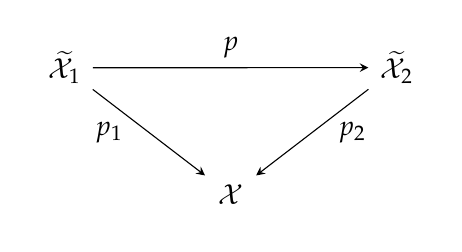
\begin{tikzpicture}
\matrix (m) [matrix of math nodes,row sep=3em,column sep=4em,minimum width=2em]
{
	\widetilde{\mathcal X}_1 & &\widetilde{\mathcal X}_2\\ 
	& {\mathcal X}\\};
\path[-stealth]
(m-1-1) edge node [above] {$p$} (m-1-3)
(m-1-1) edge node [left]  {$p_1~~$} (m-2-2)
(m-1-3) edge node [right] {$~~p_2$} (m-2-2);
\end{tikzpicture}
\\
where $\sX$ is locally connected and $p_1$, $p_2$ are covering projections. If $p$ is a surjection then $p$ is a covering projection.
\end{corollary}
\begin{theorem}\label{top_locally_conn_cov_com_thm}\cite{spanier:at}
	If   $p: \widetilde{\mathcal X}\to {\mathcal X}$ is a covering projection onto locally connected base space, then for any component  $\widetilde{\mathcal Y}$ of $\widetilde{\mathcal X}$ the map
	$$
	p|_{\widetilde{\mathcal Y}}:\widetilde{\mathcal Y} \to p\left(\widetilde{\mathcal Y} \right) 
	$$
	is a covering projection onto some component of $\widetilde{\mathcal X}$.
\end{theorem}
%\begin{lemma}\label{top_cov_cat_lem}
%In the {category of connected covering spaces} of a connected locally path-connected space every morphism is itself a covering projection.
%\end{lemma}
\begin{theorem}\label{top_conjugate_thm}\cite{spanier:at}
Let $p_1: 	\widetilde{\sX}_1 \to \sX$, $p_2: 	\widetilde{\sX}_2 \to \sX$ be objects  in the category of connected covering spaces of a connected locally path-connected space $\sX$. The following are equivalent
\begin{enumerate}
	\item [(a)] There is a coveting projection $f:\widetilde{\sX}_1 \to \widetilde{\sX}_2$ such that $p_2 \circ f = p_1$.
	\item[(b)] For all $\widetilde{x}_1\in \widetilde{\sX}_1$ and  $\widetilde{x}_2\in \widetilde{\sX}_2$ such that $p_1\left(\widetilde{x}_1 \right) = p_2\left(\widetilde{x}_2 \right)$, $\pi_1\left(p_1\right)\left( \pi_1 \left( \widetilde{\sX}_1, \widetilde{x}_1\right)  \right)$ is conjugate to a subgroup of  $\pi_1\left(p_2\right)\left( \pi_1 \left( \widetilde{\sX}_2, \widetilde{x}_2\right)  \right)$.
	\item[(c)] There exist $\widetilde{x}_1\in \widetilde{\sX}_1$ and  $\widetilde{x}_2\in \widetilde{\sX}_2$ such that $\pi_1\left(p_1\right)\left( \pi_1 \left( \widetilde{\sX}_1, \widetilde{x}_1\right)  \right)$ is conjugate to a subgroup of  $\pi_1\left(p_2\right)\left( \pi_1 \left( \widetilde{\sX}_2, \widetilde{x}_2\right)  \right)$.
\end{enumerate} 
\end{theorem}
\begin{lemma}\label{top_om_lem}\cite{spanier:at}
A local homeomorphism is an open map.
\end{lemma}
\subsection{Unique path lifting}
  \begin{empt}
	There is a significant problem in the algebraic topology, called the lifting problem. Let $p: \mathcal{E} \to \mathcal{B}$ and $f: \mathcal{X} \to \mathcal{B}$ continuous maps of topological spaces. The {\it lifting problem} \cite{spanier:at} for $f$ is to determine whether there is a continuous map $f': \mathcal{X} \to \mathcal{E}$ such that $f=p\circ f'$-that is, whether the dotted arrow in the diagram
	\newline
	\hspace*{\fill}
	\begin{tikzpicture}
	\matrix (m) [matrix of math nodes,row sep=3em,column sep=4em,minimum width=2em] {
		& \mathcal{E} \\
		\mathcal{X} & \mathcal{B} \\};
	\path[-stealth]
	(m-2-1.east|-m-2-2) edge node [below] {$f$}(m-2-2)
	(m-1-2) edge node [right] {$p$} (m-2-2)
	(m-2-1)      edge [dashed]  node[above] {$f'$} (m-1-2);
	\end{tikzpicture}
	\hspace{\fill}
	\newline
	corresponds to a continuous map making the diagram commutative. If there is such map $f'$, then $f$ can be {\it lifted} to $\mathcal{E}$, and we call $f'$ a {\it lifting} or {\it lift} of $f$.
	If $p$ is a covering projection and $\mathcal{X} = [0,1] \subset \mathbb{R}$ then $f$ can be lifted.
\end{empt}
\begin{defn}\label{top_path_lifting_defn}\cite{spanier:at}
	A continous map $p:\mathcal{E} \to \mathcal{B}$ is said to have the {\it unique path lifting} if, given paths $\omega$ and $\omega'$ in $E$ such that $p \circ \omega = p \circ \omega'$ and $\omega(0)=\omega'(0)$, then $\omega=\omega'$.
\end{defn}
\begin{thm}\cite{spanier:at}\label{spanier_thm_un}
	Let $p: \widetilde{\mathcal{X}} \to \mathcal{X}$ be a covering projection and let $f, g: \mathcal{Y} \to \widetilde{\mathcal{X}}$ be liftings of the same map (that is, $p \circ f = p \circ g$). If $\mathcal{Y}$ is connected and $f$ agrees with g for some point of $\mathcal{Y}$ then $f=g$.
\end{thm}
\begin{rem}
	From theorem \ref{spanier_thm_un} it follows that a covering projection has unique path lifting.
\end{rem}

 	\subsection{Regular and universal coverings}
 		\begin{defn}\label{top_regular_defn}\cite{spanier:at}
 		A fibration $p: \mathcal{\widetilde{X}} \to \mathcal{X}$ with unique path lifting is said to be  {\it regular} if, given any closed path $\omega$ in $\mathcal{X}$, either every lifting of $\omega$ is closed or none is closed.
 	\end{defn}
 	\begin{thm}\label{locally_path_thm}\cite{spanier:at}
 		Let $p: \widetilde{\mathcal X} \to \mathcal X$ be a fibration with unique path lifting and assume that a nonempty $\widetilde{\mathcal X}$ is a locally path-connected space. Then $p$ is regular if and only if for some $\widetilde{x}_0 \in  \widetilde{\mathcal X}$, $\pi_1\left(p\right)\pi_1\left(\widetilde{\mathcal X}, \widetilde{x}_0\right)$ is a normal subgroup of $\pi_1\left(\mathcal X, p\left(\widetilde{x}_0\right)\right)$.
 	\end{thm}
 	\begin{theorem}\label{top_cov_fact_thm}\cite{spanier:at}
 		Let $G$ be a properly discontinuous group of homeomorphisms of space $\mathcal Y$. Then the projection of $\mathcal Y$ to the orbit space $\mathcal Y/G$ is a covering projection. If $\mathcal Y$ is connected, this covering is regular and $G$ is its group of covering transformations, i.e. $G = G\left(\mathcal Y~|~\mathcal Y/G \right)$. 
 	\end{theorem}
 	\begin{lem}\label{top_cov_from_pi1_cor}\cite{spanier:at}
 		Let $p: \widetilde{\mathcal X} \to \mathcal X$ be a fibration with a unique path lifting. If $ \widetilde{\mathcal X}$ is connected and locally path-connected and $\widetilde{x}_0 \in \widetilde{\mathcal X}$ then $p$ is regular if and only if $G\left(\widetilde{\mathcal X}~|~{\mathcal X} \right)$ transitively acts on each fiber of $p$, in which case 
 		$$
 		\psi: G\left(\widetilde{\mathcal X}~|~{\mathcal X} \right) \approx \pi_1\left(\mathcal X, p\left( \widetilde{x}_0\right)  \right) / \pi_1\left( p\right)\pi_1\left(\widetilde{\mathcal X}, \widetilde{x}_0 \right).  
 		$$
 	\end{lem}
 \begin{remark}\label{top_sim_con_reg_rem}\cite{spanier:at}
 If $\widetilde{   \sX}$ is simply connected, any fibration $p: \widetilde{   \sX} \to \sX$ is regular, and we also have the next result.
 \end{remark}
 	\begin{cor}\label{top_cov_pi1_cor}\cite{spanier:at}
 		Let $p: \widetilde{\mathcal X} \to \mathcal X$ be a fibration with a unique path lifting where $ \widetilde{\mathcal X}$ is simply connected locally path-connected and nonempty.  Then the group of self-equivalences of $p$ is isomorphic to the fundamental group of ${\mathcal X}$, i.e. $\pi_1\left( {\mathcal X}\right)\approx G\left(\left.\widetilde{\sX}~\right|\sX\right)$.  
 	\end{cor}
 \begin{definition}\label{top_uni_cov_defn}\cite{spanier:at}
 	A \textit{universal covering space} of a connected space $\sX$ is an object $p: \widetilde{\sX}\to \sX$ of the category of connected covering spaces of $\sX$ such that for any object $p': \widetilde{\sX}'\to \sX$ of this category there is a morphism 
 	\newline
 	\begin{tikzpicture}
 	\matrix (m) [matrix of math nodes,row sep=3em,column sep=4em,minimum width=2em]
 	{
 		\widetilde{\sX}  &  & \widetilde{\sX}'\\
 		& \sX & \\};
 	\path[-stealth]
 	(m-1-1) edge node [above] {$f$} (m-1-3)
 	(m-1-1) edge node [left]  {$p~~$} (m-2-2)
 	(m-1-3) edge node [right] {$~~p'$} (m-2-2);
 	%\draw[dashed,->]   (m-1-1) -- (m-1-3);
 	\end{tikzpicture}
 	\\
 	in the category.
 \end{definition}
 
 \begin{lem}\label{top_simply_con_cov_lem}\cite{spanier:at}
 	A connected locally path-connected space $\mathcal X$ has a simply connected covering space if and only if  $\mathcal X$ is semilocally 1-connected.
 \end{lem}
 %\begin{lem}\label{top_simply_con_uni_cor}\cite{spanier:at}
 %	Any universal covering space of a connected locally path connected semilocally 1-connected space is simply connected.
% \end{lem}
 %\begin{lem}\label{top_uni_spa_lem}\cite{spanier:at}
% 	Two universal covering spaces of a connected locally path-connected space are equivalent.
% \end{lem}
 
  \begin{lem}\label{top_uni_exist_spa_lem}\cite{spanier:at}
 A simply connected covering space of a connected locally path-connected space $\sX$ is an universal covering space of $\sX$.
 \end{lem}
 
 
 	\section{Vector bundles}\label{top_vb_sub_sub}
 	\begin{definition}\cite{karoubi:k}
 		A \textit{quasi-vector bundle with base} $\mathcal X$ is given by:
 		\begin{enumerate}
 			\item [(a)] A finite dimensional $\C$-vector space $E_x$ for every point $x$ of $\mathcal X$.
 			\item[(b)] A topology on the disjoint union $E = \bigsqcup E_x$ which induces the natural topology on each $E_x$, such that the obvious projection $\pi: E \to  \mathcal X$ is continuous.
 		\end{enumerate}
 		The quasi-vector bundle with base will be denoted by $\left( E, \pi, \mathcal X\right)$.
 	\end{definition}
 	\begin{remark}
 		In \cite{karoubi:k} the vector bundles over fields $\R$ and $\C$ are considered. Here we consider complex vector bundles only.
 	\end{remark}
 	We refer to \cite{karoubi:k} for a notion of {\it (locally trivial) vector bundle}.
 	Any {\it (locally trivial) vector bundle} with base $\mathcal X$ is a special case of \textit{quasi-vector bundle} which is a triple $\left(E, \pi, \mathcal X \right)$. 
 	\begin{definition}\label{vb_inv_img_funct_defn}\cite{karoubi:k}
 		Let $f: \mathcal X' \to \mathcal X$ be a continuous map. For every point $x'$ of $\mathcal X'$, let $E'_{x'}= E_{f\left(x' \right) }$. Then the set $E' = \bigsqcup_{x' \in \mathcal X'}$ may be identified with the \textit{fiber product} $\mathcal X' \times_{\mathcal X} E$ formed by the pairs $\left(x',e \right)$ such that $f\left(x' \right) = \pi\left( e\right)$. If  $\pi': E' \to \mathcal X'$ is defined by $\pi'\left(x',e \right) = x'$, it is clear that the triple $\xi = \left( E', \pi', \mathcal X'\right)$ defines a quasi-vector bundle over $ \mathcal X'$, when we provide $E'$ with the topology induced by $ \mathcal X' \times E$. We write $\xi' = f^*\left(\xi \right)$ or $f^*\left(E \right)$: this is the \textit{inverse image} of $\xi$ by $f$.  
 	\end{definition}
 	We refer to \cite{karoubi:k} for a notion of {\it (locally trivial) vector bundle}.
 	\begin{definition}\label{vb_cont_sec_defn}
 		If $\left( E, \pi, \mathcal X\right)$ is a quasi-vector bundle then a continuous map $s: \mathcal X\to E$ is said to be a \textit{continuous section} if $\pi \circ s = \Id_{ \mathcal X}$.  The space $\Ga\left({\mathcal X}, {E}\right)$, of continuous sections can be regarded as both left and right $C_b\left(\mathcal{X} \right)$-module.
 	\end{definition}
 	
 	%\begin{definition}\label{vb_inv_img_funct_defn}
 	%	If $f: \mathcal X \to \mathcal Y$ is a continuous map then there is an {\it inverse image functor}  $f^*:\mathrm{Vect}(\mathcal{Y})\to\mathrm{Vect}(\mathcal{X})$ (cf. \cite{karoubi:k}). 
 	%\end{definition}
 	
 	
 	
 	%Following fact is an implication of definitions.
 	%\begin{fact}\label{inv_image_fact}
 	%	A map $\varphi^*$ is an inverse image of $\varphi$ if and only if the above diagram is commutative for any $\mathcal U$ such that $\pi |_{\mathcal U}: \mathcal U \to \pi ({\mathcal U})$ is a homeomorphism.
 	%\end{fact}
 	
 	\begin{empt}\label{top_herm_bundle_empt}
 		Let $\mathcal X$ be a topological space and $S$ the complex vector bundle on $\mathcal X$, such for any  $x \in \mathcal{X}$ the fiber $S_x$ of $S$ is a Hilbert space, i.e. there is a scalar product.
 		\be\label{top_bundle_scalar_eqn}
 		\left( \cdot, \cdot \right)_x: S_x \times S_x \to \C.
 		\ee
 		 If $\Ga\left( M, S\right) $ is the space of continuous sections
 		of $S$ then we suppose that for any $\xi, \eta \in  \Ga\left( M, S\right)$ the map $\mathcal X \to \C$ given by $x \mapsto \left( \xi_x, \eta_x\right)_x$ is continuous. If    $\mu_{\mathcal{X}}$ is a measure on $\mathcal X$ then there is the scalar product $\left( \cdot, \cdot \right) :  \Ga\left( M, S\right) \times \Ga\left( M, S\right) \to \C$ given by
 	\be\label{top_bundle_herm_scalar_eqn}
 		\left( \xi, \eta\right)\stackrel{\text{def}}{=} \int_{\mathcal X}\left( \xi_x, \eta_x\right)_xd~\mu_{\mathcal{X}}
 	\ee
 		Denote by $L^2\left( \mathcal X, S, \mu_{\mathcal X}\right) $ or $L^2\left( \mathcal X, S\right) $ the Hilbert norm completion of $\Ga\left( M, S\right) $, and denote by $\left( \cdot, \cdot \right)_{L^2\left( \mathcal X, S, \mu_{\mathcal X}\right)}$ or $\left( \cdot, \cdot \right)_{L^2\left( \mathcal X, S\right)}$ the given by \eqref{top_bundle_herm_scalar_eqn} scalar product.
 		There is the natural representation
 		\begin{equation}\label{comm_bundle_repr_eqn}
 		C_0\left(\mathcal{X} \right) \to B\left( L^2\left( \mathcal X, S\right)\right). 
 		\end{equation}
 	\end{empt}
 	\begin{defn}\label{top_herm_bundle_defn}
 		In the situation of \ref{top_herm_bundle_empt} we say that $S$ is \textit{Hermitian vector bundle}.
 	\end{defn}
 \begin{remark}\label{top_herm_cont_rem}
 If $\left(\sS, \pi, \sX \right)$ is a Hermitian vector bundle then for all $x \in \sX$ one can define the norm on $\sS_x$
 \be\label{top_herm_norm_eqn}
 \left\| \xi_x\right\| = \sqrt{	\left( \xi_x,\xi_x \right)_x}
 \ee 
 If $\xi \in \Ga\left(\sX, \sE\right)$ then 
 \be\label{top_herm_cont_eqn}
 \left(x \mapsto \left\| \xi_x\right\| \right) \in C_b\left(\sX \right) 
 \ee
 \end{remark}
 
 \chapter{Algebra}
 \section{Algebraic Morita equivalence}
 
 \begin{defn}\label{morita_ctx_defn}
 	A \textit{Morita context} $\left( A,B,P,Q,\varphi,\psi\right)$ or, in some authors (e.g. Bass \cite{bass}) the \textit{pre-equivalence data} is a generalization of Morita equivalence between categories of modules. In the case of right modules, for two associative $\mathbf{k}$-algebras (or, in the case of $\mathbf{k} = \mathbb{Z}$, rings) $A$ and $B$, it consists of bimodules $_AP_B$, $_BQ_A$ and bimodule homomorphisms $\varphi: P\otimes_B Q\to A$, $\psi: Q\otimes_A P\to B$ satisfying mixed associativity conditions, i.e. for any $p,p' \in P$ and $q,q' \in Q$ following conditions hold:
 	\begin{equation}\label{morita_ctx_eqn}
 	\begin{split}
 	\varphi\left(p\otimes q \right) p' = p \psi\left(q\otimes p' \right),\\
 	\psi\left(q \otimes p \right) q' = q\varphi\left(p\otimes q' \right).  
 	\end{split}
 	\end{equation}
 	A Morita context is a \textit{Morita equivalence} if both $\varphi$ and $\psi$ are isomorphisms of bimodules. 
 \end{defn}
 
 \begin{rem}\label{morita_rem}
 	The Morita context $\left( A,B,P,Q,\varphi,\psi\right)$  is a Morita equivalence if and only if $A$-module $P$ is a finitely generated projective generator (cf. \cite{bass} II 4.4)
 \end{rem}
 
% \begin{cordefn}\label{invert_mod_defn}\cite{bass}
% 	Let $R$ be a commutative ring, and let $A$, $B$ be $R$-algebras
% 	We call a left $A\otimes_RB^\circ$ module $M$ \textit{invertible} if it satisfies to the following conditions, which are equivalent:
% 	\begin{enumerate}
% 		\item [(a)] $\otimes_{A}M:~ mod$-$A \xrightarrow{\approx} mod$-$B$ is an equivalence.
% 		\item[(b)] There is a left left $B\otimes_RA^\circ$ module $N$ such that $M\otimes_BN \cong A$ and $N\otimes_AM \cong B$ as bimodules.
% 		\item [(c)] $M\otimes_{B}:~B$-$mod \xrightarrow{\approx} ~B$-$mod$ is an equivalence.
% 	\end{enumerate}
 %\end{cordefn}
% \begin{empt}\label{invert_mod_auto_empt}\cite{bass}
% 	For any $R$-algebra $A$ write $\mathbf{Pic}_R\left(A \right)$  for the category of invertible $A\otimes_RA^\circ$ modules and bimodule isomorphisms. For any $\al, \bt \in \Aut_{R\mathrm{-alg}}\left(A \right)$ denote by $_\al A_\bt$ the $A\otimes_RA^\circ$ module such that there is $R$-linear isomorphism $\varphi: A \xrightarrow{\approx}_\al A_\bt$ and following condition holds
% 	\be\label{pic_act_eqn}
% 	a\varphi\left(x \right)b = \varphi\left(\al\left(a \right) x\bt\left(b\right)  \right); \quad \forall a, x, b \in A. 
% 	\ee	
% \end{empt}
 
% \begin{proposition}\label{invert_mod_auto_prop}
% 	Let $A$ be an $R$-algebra and let  $\al, \bt, \ga \in \Aut_{R\mathrm{-alg}}\left(A \right)$.
 %	\begin{enumerate}
 %		\item [(i)] $_\al A_\bt \cong _{\ga\al} A_{\ga\bt}$ as bimodules.
% 		\item[(ii)] $_{\Id_A} A_{\al}\otimes_A ~_{\Id_A} A_{\al} \cong _{\Id_A} A_{\al\bt}$ as bimodules.
% 		\item[(iii)] 
% 		$$
% 		_{\Id_A} A_{\al} \cong _{\Id_A}A_{\Id_A} \Leftrightarrow \al \mathrm{~is~an~inner~automorphism}.
% 		$$
 %		\item[(iv)] If $P \in \mathbf{Pic}_R\left(A \right)$ and if $P\cong A$ as left $A$-modules then $P\cong _{\Id_A} A_{\al}$ as bimodules for some $\al \in  \Aut_{R\mathrm{-alg}}\left(A \right)$.
% 	\end{enumerate}
% \end{proposition}

		\section{Finite Galois coverings}\label{fin_gal_cov_sec}
\paragraph*{} Here I follow to \cite{auslander:galois}. Let $A \hookto \widetilde{A}$ be an injective homomorphism of unital algebras, such that
\begin{itemize}
	\item $\widetilde{A}$ is a projective finitely generated $A$-module,
	\item There is an action $G \times \widetilde{A} \to \widetilde{A}$ of a finite group $G$ such that $$A = \widetilde{A}^G=\left\{\widetilde{a}\in \widetilde{A}~|~g\widetilde{a}=\widetilde{a}; ~\forall g \in G\right\}.$$
\end{itemize}
Let us consider the category $\mathscr{M}^G_{\widetilde{A}}$ of $G-\widetilde{A}$ modules, i.e.  any object $M \in \mathscr{M}^G_{\widetilde{A}}$ is a $\widetilde{A}$-module with equivariant action of $G$, i.e. for any $m \in M$ a following condition holds
$$
g\left(\widetilde{a}m \right)=  \left(g\widetilde{a} \right) \left(gm \right) \text{ for any } \widetilde{a} \in \widetilde{A}, ~ g \in G.
$$
Any morphism $\varphi: M \to N$ in the category $\mathscr{M}^G_{\widetilde{A}}$ is $G$- equivariant, i.e.
$$
\varphi\left( g m\right)= g \varphi\left( m\right)   \text{ for any } m \in M, ~ g \in G.
$$
Let $\widetilde{A}\left[ G\right]$ be an algebra such that $\widetilde{A}\left[ G\right] \approx \widetilde{A}\times G$ as an Abelian group and a multiplication law is given by
$$
\left( a, g\right)\left( b, h\right) =\left(a\left(gb \right), gh  \right).
$$
The category $\mathscr{M}^G_{\widetilde{A}}$ is equivalent to the category $\mathscr{M}_{\widetilde{A}\left[ G\right]}$ of $\widetilde{A}\left[ G\right]$ modules. Otherwise in \cite{auslander:galois} it is proven that if $\widetilde{A}$ is a finitely generated, projective $A$-module then there is an  equivalence between a category $\mathscr{M}_{A}$ of $A$-modules and the category $\mathscr{M}_{\widetilde{A}\left[ G\right]}$. It turns out that the category $\mathscr{M}^G_{\widetilde{A}}$ is equivalent to the category $\mathscr{M}_{A}$. The equivalence is given by mutually inversed functors $\left( -\right) \otimes \widetilde{A}: \mathscr{M}_{A} \to \mathscr{M}^G_{\widetilde{A}}$ and $\left( -\right) ^G: \mathscr{M}^G_{\widetilde{A}}\to \mathscr{M}_{A}$.






\section{Profinite and residually finite groups}\label{profinite_section}
\begin{empt}\label{prof_empt}\cite{dix:profinite}
	Let $G$ be a group and $\left\{G_\al \right\}$ be the set of all normal subgroups of finite index in $G$. Then the set $\left\{G/G_\al, \phi_{\al\bt}\right\}$ of finite quotients $G/G_\al$, of $G$ together with the canonical projections $\phi_{\al\bt}:G/G_\al \to G/G_\bt$  whenever $G_\al \subset G_\bt$ is an inverse system. The inverse limit $\varprojlim G/G_\a$ of this system is called the \textit{profinite completion} of $G$ and is denoted by $\widehat{G}$. The group $\widehat{G}$ can also be described as the closure of the image of $G$ under the
	the diagonal mapping $\Delta : G \to \prod \left( G/G_\a\right)$  where $G/G_\a$, is given the discrete topology and $\prod \left( G/G_\a\right)$ has the product topology. In this description the elements of $\widehat{G}$ are the
	elements $\left(g_\a \right) \in \prod \left( G/G_\a\right)$ which satisfy $\phi_{\al\bt}\left( g_\al\right)= \bt$  whenever $G_\a \subset G_\bt$.
\end{empt} 
%\begin{theorem}\label{profinite_thm}\cite{dix:profinite}
%	Let $G$ and $H$ be finitely generated groups, and let $\widehat{G}$ (resp. $\widehat{H}$) be the profinite completion of $G$ (resp. $H$), Then $\widehat{G}$ and $\widehat{H}$ are isomorphic as topological groups id the set of isomorphism classes of finite quotients  of $G$ is equal the set of isomorphism classes of finite quotients  of $H$.
%\end{theorem}

\begin{definition}\label{residually_finite_defn}\cite{bogopolsky:group_theory}
	A group $G$ is said to be \textit{residually finite} if for each nontrivial element from $G$ there exists a finite group $K$ and a homomorphism $\varphi: G\to K$ such that $\varphi\left( g\right) \neq 1$.
\end{definition}

%\section{Miscellany}

% \begin{theorem}\label{noeter_skolem_thm}\cite{pierce:ass}
% Let $F$ be a field, and let $A$ be a finite-dimensional simple central $F$-algebra. Suppose that $B$ is a simple subalgebra of $A$. If $\chi$ is an algebra homomorphism of $B$ to $A$ then there exists an invertible element $u \in A$ such that $\chi\left(y \right) = u^{-1}yu$ for all $y \in B$.
% \end{theorem}
 
 
 %\begin{theorem}[Morita \cite{Morita:58}, \cite{Morita:65}]
 %	\label{the:ProGenMorita}
 %	Let~$R$ be a ring with unit and~$Q$ a right $R$-module.  Then~$Q$ induces a
 %	Morita equivalence between~$R$ and $R'\subset\End(Q)$ if and only if~$Q_R$ is
 %	a finitely generated projective generator.%\footnote{An object~$X$ in an 		Abelian category is a generator iff every object is a quotient of a direct 		sum of copies of~$X$.}
 %\end{theorem}
 
 
 
 	
	\chapter{Operator algebras}	
 	\section{$C^*$-algebras and von Neumann algebras}
 	\paragraph{}In this section I follow to \cite{murphy,pedersen:ca_aut}.
 	\begin{defn}\label{strict_topology}\cite{pedersen:ca_aut}
 		Let $A$ be a $C^*$-algebra.  The {\it strict topology} on the multiplier algebra $M(A)$ is the topology generated by seminorms $\vertiii{x}_a = \|ax\| + \|xa\|$, ($a\in A$). We denote by $\bt\text{-}\lim$ the limit with respect to the strict topology.
 		If $x \in M(A)$  and a sequence of partial sums $\sum_{i=1}^{n}a_i$ ($n = 1,2, ...$), ($a_i \in A$) tends to $x$ in the strict topology then we shall write
 		\begin{equation*}
 		x = \bt\text{-}\lim\sum_{i=1}^{\infty}a_i.
 		\end{equation*}
 	\end{defn}
 \begin{defn}\label{unitization_defn}\cite{rae:ctr_morita}
 A \text{unitization} of a $C^*$-algebra $A$ is  a $C^*$-algebra $B$ with identity and an injective *-homomorphism $\iota: A \hookto B$ such that $\iota\left(A\right)$ is an essential ideal of $B$. 
 \end{defn}
\begin{example}\label{unitization_exm}
Suppose A is a $C^*$-algebra which has no identity. Then $A^+ = A \oplus \C$
is a *-algebra with 
$$
\left( a \oplus \la\right)\left( b \oplus \mu\right) = \left(ab + \la b + \mu a\right)  \oplus \la \mu, \quad \left(a \oplus \la \right)^* = a^*\oplus \overline{\la}. 
$$
It is proven in \cite{rae:ctr_morita} that there is the natural unique $C^*$-norm $\left\| \cdot\right\|_{A^+}$  on $A^+$ such that 
$$
\left\|a \oplus 0 \right\|_{A^+}=\left\|a \oplus 0 \right\|_{A}
$$
where $\left\|\cdot \right\|_{A}$ is the $C^*$-norm on $A$.
\end{example}
\begin{definition}\label{multiplier_min_defn}
	Let $A$ be a $C^*$-algebra. A unitization   $\iota: A \hookto B$  is called \textit{minimal} if following conditions hold:
	\begin{itemize}
		\item If $A$ is not unital then $B = A^+$ where $A^+$ is described in the example \ref{unitization_exm}.
		\item If $A$ is  unital then $B = A$ and $\iota = \Id_A$.
	\end{itemize}
The minimal unitization will be denoted by $A^+$.
\end{definition}
\begin{definition}\label{multiplier_max_defn}\cite{rae:ctr_morita}
A unitization   $\iota: A \hookto B$  is called \textit{maximal} if for every embedding $j$ of $A$ as an essential ideal of a $C^*$-algebra $\phi: C\to B$ such that $\phi \circ j = \iota$. 
\end{definition}

\begin{rem}\label{multiplier_rem}
It is proven in \cite{rae:ctr_morita} that for any $C^*$-algebra $A$ there unique maximal unitization
\end{rem}

\begin{definition}\label{multiplier_defn}
	We say that the maximal unitization of $A$ is the \textit{multiplier algebra} of $A$ and denote it by $M\left( A\right)$. 
\end{definition}
 \begin{defn}\label{app_unit_defn}\cite{pedersen:ca_aut}
	Let $A$ be a $C^*$-algebra. A net $\left\{u_\la \right\}_{\la \in \La}$ in $A_+$ with $\left\|u_\la \right\| \le 1$ for all $\la \in \La$ is called an \textit{approximate unit} for $A$ if $\la < \mu$ implies $u_\la < u_\mu$ and if $\lim \left\|x- xu_\la \right\| = 0$ for each $x$ in $A$. Then, of course, $\lim \left\|x- u_\la x \right\| = 0$ as well.
\end{defn}
 \begin{proposition}\label{mult_str_pos_prop}\cite{apt_mult}
 	If $B$ is a $C^*$-subalgebra of $A$ containing an
 	approximate unit for $A$, then  $M\left(B \right) \subset M\left( A\right)$  (regarding $B''$ as a subalgebra	of $A''$).
 \end{proposition}
\begin{definition}\label{hered_defn}\cite{pedersen:ca_aut}
	A cone in the positive part of $C^*$-algebra $A$ is said to be \textit{hereditary} if $0 \le x \le y$, $y \in M$ implies $x \in M$ for each $x \in A$. A *-subalgebra $B$ of $A$ is \textit{hereditary} if $B_+$ is hereditary in $A_+$.
\end{definition}
\begin{lemma}\label{hered_lem}\cite{murphy}
Let $B$ be a $C^*$-subalgebra of $C^*$-algebra $A$. Then $B$ is hereditary in $A$ if and only if $bab' \in B$ for all $b, b' \in B$ and $a \in A$.
\end{lemma}
\begin{lemma}\label{hered_ideal_lem}\cite{murphy}
	\begin{enumerate}
		\item[(i)] If $L$ is a closed left ideal in $A$ then $L\cap L^*$ is a hereditary $C^*$-subalgebra of $A$. The map $L \mapsto L\cap L^*$ is the bijection from the set of closed left ideals of $A$ onto the the set of hereditary $C^*$-subalbebras of $A$.
		\item[(ii)] If $L_1, L_2$ are closed left ideals, then $L_1 \subseteq L_2$ is and only if $L_1\cap L_1^* \subset L_2\cap L_2^*$.
		\item[(iii)] If $B$ is a hereditary $C^*$-subalgebra of $A$, then the set 
		$$
		L\left(B \right) = \left\{\left.a \in A~\right| a^*a \in B \right\}
		$$
		is the unique closed left ideal of $A$ corresponding to $B$.
			\end{enumerate}
\end{lemma}

 	\begin{defn}\label{center_defn}\cite{murphy}
 		If $A$ is a $C^*$-algebra, its \textit{center} $C$ is the set of elements of $A$ commuting with every of $A$.
 	\end{defn}
 	\begin{defn}
 		\label{strong_topology_defn}\cite{pedersen:ca_aut} Let $\H$ be a Hilbert space. The {\it strong} topology on $B\left(\H\right)$ is the locally convex vector space topology associated with the family of seminorms of the form $x \mapsto \|x\xi\|$, $x \in B(\H)$, $\xi \in \H$.
 	\end{defn}
 	\begin{defn}\label{weak_topology_defn}\cite{pedersen:ca_aut} Let $\H$ be a Hilbert space. The {\it weak} topology on $B\left(\H\right)$ is the locally convex vector space topology associated with the family of seminorms of the form $x \mapsto \left|\left(x\xi, \eta\right)\right|$, $x \in B(\H)$, $\xi, \eta \in \H$.
 	\end{defn}
 	
 	\begin{thm}\label{vN_thm}\cite{pedersen:ca_aut}
 		Let $M$ be a $C^*$-subalgebra of $B(\H)$, containing the identity operator. The following conditions are equivalent:
 		\begin{itemize}
 			\item $M=M''$ where $M''$ is the bicommutant of $M$;
 			\item $M$ is weakly closed;
 			\item $M$ is strongly closed.
 		\end{itemize}
 	\end{thm}
 	
 	\begin{defn}
 		Any $C^*$-algebra $M$ is said to be a {\it von Neumann algebra} or a {\it $W^*$- algebra} if $M$ satisfies to the conditions of the Theorem \ref{vN_thm}.
 	\end{defn}
 	\begin{defn} \cite{pedersen:ca_aut}
 		Let $A$ be a $C^*$-algebra, and let $S$ be the state space of $A$. For any $s \in S$ there is an associated representation $\pi_s: A \to B\left( \H_s\right)$. The representation $\bigoplus_{s \in S} \pi_s: A \to \bigoplus_{s \in S} B\left(\H_s \right)$ is said to be the \textit{universal representation}. The universal representation can be regarded as $A \to B\left( \bigoplus_{s \in S}\H_s\right)$.  
 	\end{defn} 
 	\begin{defn}\label{env_alg_defn}\cite{pedersen:ca_aut}
 		Let   $A$ be a $C^*$-algebra, and let $A \to B\left(\H \right)$ be the universal representation $A \to B\left(\H \right)$. The strong closure of $\pi\left( A\right)$ is said to be   the  {\it enveloping von Neumann algebra} or  the {\it enveloping $W^*$-algebra}  of $A$. The enveloping  von Neumann algebra will be denoted by $A''$.
 	\end{defn}
 	\begin{prop}\label{env_alg_sec_dual}\cite{pedersen:ca_aut}
 		The enveloping von Neumann algebra $A''$ of a $C^*$-algebra $A$ is isomorphic, as a Banach space, to the second dual of $A$, i.e. $A'' \approx A^{**}$.
 	\end{prop}
 	
 	\begin{thm}\label{env_alg_thm}\cite{pedersen:ca_aut}
 		For each non-degenerate representation $\pi: A \to B\left(\H \right)$ of a $C^*$-algebra $A$ there is a unique  normal morphism of  $A''$ onto $\pi\left( A\right)''$ which extends $\pi$.   
 	\end{thm}
 	
 	
 	
 	%\begin{defn}\cite{pedersen:ca_aut}
 	%Let $B \in B(H)$ be a $C^*$-algebra. Denote by $B''$ the strong closure of $B$ in $B(H)$. $B''$ is an unital weakly closed $C^*$-algebra and if $B$ acts non-degenerately on $H$ then  $B''$ is the {\it bicommutant} of $B$. Any strongly (=weakly) closed algebra is said to be a {\it von Neumann algebra}.
 	%\end{defn}
 	%\begin{defn}\cite{pedersen:ca_aut}
 	%For any $x\in B(H)$ element $|x| \stackrel{\text{def}}{=} (xx^*)^{1/2}$ is said to be the {\it absolute value of} $x$.
 	%\end{defn}
 	\begin{lem}\label{increasing_convergent_w_lem}\cite{pedersen:ca_aut} Let $\Lambda$ be an increasing in the partial ordering.  Let $\left\{x_\lambda \right\}_{\la \in \La}$ be an increasing of self-adjoint operators in $B\left(\H\right)$, i.e. $\la \le \mu$ implies $x_\la \le x_\mu$. If $\left\|x_\la\right\| \le \ga$ for some $\ga \in \mathbb{R}$ and all $\la$ then $\left\{x_\lambda \right\}$ is strongly convergent to a self-adjoint element $x \in B\left(\H\right)$ with $\left\|x_\la\right\| \le \ga$.
 	\end{lem}
 	%\begin{defn}\label{range_proj_defn}\cite{pedersen:ca_aut}
 	%For each $x\in B(\H)$ we define the {\it range projection} of $x$ (denoted by $[x]$) as projection on closure of $x\H$. If $x\ge 0$ then the sequence $\left(\left((1 /n) +x\right)^{-1}x\right)$ is monotone increasing to $[x]$.  If $p$ and $q$ are projections then $p \vee q = [p + q]$ and thus $p \wedge q = 1 - \left[2 - \left(p+q\right)\right]$. Similarly we have $p \setminus q = p - p\wedge q$. Since $[x]\H$ is the orthogonal complement of the null space of $x^*$ we have $[x]=[xx^*]$. 
 	%\end{defn}
 	%\begin{cor}
 	%If $M$ is a $W^*$-algebra and $a \in M$ then the range projection $[a]$ of $a$ lies in $M$.
 	%\end{cor}
 	%If $\mathcal{M}$ is a von Neumann algebra in $B(\H)$ then $[x]\in \mathcal{M}$ for any $x\in \mathcal{M}$. We next prove a {\it polar decomposition}.
 	\paragraph*{}    For each $x\in B(\H)$ we define the {\it range projection} of $x$ (denoted by $[x]$) as projection on the closure of $x\H$. If $M$ is a von Neumann algebra and $x \in M$ then $[x]\in M$.
 	
 	\begin{prop}\label{polar_decomposition_prop}\cite{pedersen:ca_aut}
 		For each element $x$ in   a von Neumann algebra $M$ there is a unique partial isometry $u\in M$ and positive $\left|x\right| \in M_+$ with $uu^*=[|x|]$ and  $x=|x|u$.
 	\end{prop}
 	\begin{defn}\label{polar_decomposition_defn}
 		The formula $x=|x|u$ in the Proposition \ref{polar_decomposition_prop} is said to be the \textit{polar decomposition}.
 	\end{defn}

 \begin{thm}\label{app_unit_thm}\cite{pedersen:ca_aut}
 Each $C^*$-algebra contains an \textit{approximate unit}.
\end{thm}
\begin{definition}\label{stritly_pos_defn}\cite{pedersen:ca_aut}
%2.10.4	
We say that an element $h$ is a $C^*$-algebra is \textit{strictly positive} if $\phi\left( h\right)>0$ for any nonzero positive linear functional $\phi$ on $A$.
\end{definition}
 \begin{thm}\label{stritly_pos_thm}\cite{pedersen:ca_aut}
	Let $A$ be a $C^*$-algebra. The following conditions are equivalent:
	\begin{enumerate}
		\item [(i)] There is a strictly positive element $h$ in $A_+$.
		\item[(ii)] There is an element $h$ in $A_+$ such that $\left[ h\right] = 1$ in $A''$.
		\item[(iii)] There is a countable approximate unit for $A$.
	\end{enumerate}
\end{thm}
\begin{proposition}\label{stritly_pos_prop}\cite{blackadar:ko}
%Proposition 12.3.1. 
Let $A$ be a $C^*$-algebra, and $h \in A_+$. Then $h$ is strictly
positive if and only if $hA$ is dense in $A$.
\end{proposition}

\begin{theorem}\label{irred_thm}\cite{pedersen:ca_aut}
 		Let $A \to B\left(\H \right)$ be a nonzero representation of $C^*$-algebra $A$. The following conditions are equivalent:
 		\begin{enumerate}
 			\item [(i)] There are no non-trivial subspaces for $\pi$.
 			\item[(ii)] The commutant of $\pi\left(A \right)$ is the scalar multipliers of 1.
 			\item[(iii)] $\pi\left(A \right)$ is strongly dense in   $B\left(\H \right)$.
 			\item[(iv)] For any two vectors $\xi, \eta \in \H$ with $\xi \neq 0$ there is $a \in A$ such that $\pi\left(a \right)\xi = \eta$.
 			\item[(v)] Each nonzero vector in $\H$ is cyclic for  $\pi\left(A \right)$.
 			\item[(vi)]  $A \to B\left(\H \right)$ is spatially equivalent to a cyclic representation associated with a pure state of $A$.
 		\end{enumerate} 
 	\end{theorem}
 	\begin{definition}\label{irred_defn}
 		Let $A \to B\left(\H \right)$ be a nonzero representation of $C^*$-algebra $A$. The representation is said to be \textit{irreducible} if it satisfies to the Theorem \ref{irred_thm}.
 	\end{definition}
 	\begin{remark}\label{irr_func_rem}
 		From the condition (i) of the Theorem \ref{irred_thm} it turns out that irreducibility is the categorical property, i.e. if there is the equivalence between category of representations of $C^*$-algebras then any irreducible representation is mapped to irreducible one.  The equivalence between category of representations corresponds to the strong Morita equivalence (cf. \ref{strong_morita_sec}).
 	\end{remark}
 	\begin{definition}\label{equiv_repr_defn}\cite{pedersen:ca_aut}
 		Let $A$ be a $C^*$-algebra.
 		We say that two representations $\pi_1: A \to B\left( \H_1\right)$ and $\pi_2: A \to B\left( \H_2\right)$  are \textit{spatially equivalent} (or \textit{unitary equivalent}) if there is an isometry $u$ of $\H_1$ onto $\H_2$ such that $u\pi_1\left(a \right)u^*=\pi_2\left(a \right)$ for all $a \in A$. By the \textit{spectrum} of $A$ we understand the set $\hat A$ of spatially equivalence classes of irreducible representations. For any $x \in \hat A$ we denote by
 		\be\label{rep_x_eqn}
 		\begin{split}
 			\rep_x : A \to B\left( \H\right) \quad \text{OR} \quad 	\rep^A_x : A \to B\left( \H\right)
 		\end{split}
 		\ee
 a representation which corresponds to $x$.  Sometimes we use alternative notation of the spectrum $A^\wedge\stackrel{\text{def}}{=}\hat A$.
 	\end{definition}
 	\begin{definition}\label{prim_sp_defn}
 		Let $A$ be a $C^*$-algebra.
 		The \textit{primitive spectrum} is the space of the primitive ideals of $A$, we shall denote the primitive spectrum by $\check{A}$.
 	\end{definition}
 	\begin{remark}
 		There is the natural surjective map 
 		\be\label{check_hat_eqn}
 		\hat{A}\to \check{A}
 		\ee
 		which maps an irreducible representation to its kernel.
 	\end{remark}
 	\begin{empt}
 		For each set $F$ in $\check{A}$ define a closed ideal 
 		\be\label{ker_f_eqn}
 		\ker\left( F\right) = \bigcap_{t \in F} t.
 		\ee
 		For each subset $I$ of $A$ define a set
 		\be\label{hull_eqn}
 		\mathrm{hull}\left( I\right) = \left\{t \in \check{A}~|~I \subset t \right\}
 		\ee
 		Using a surjective map $\hat A \to \check{A}$ one can define the $\mathrm{hull}\left( I\right)\subset \hat A$ as the preimage of $\mathrm{hull}\left( I\right)$ in $\check{A}$
 	\end{empt}
 	\begin{theorem}\label{jtop_thm}
 		The class $\left\{\mathrm{hull}\left( I\right)~|~I \subset A\right\}$ form the closed sets for a topology on $\check{A}$. There is a bijective order preserving isomorphism between open sets in this topology and the closed ideals in $A$.
 	\end{theorem}
 	\begin{definition}\label{jtop_defn}
 		The topology on  $\check{A}$ defined in the Theorem \ref{jtop_thm} is called be the \textit{Jacobson topology}. The topology on $\hat A$ induced by the surjecive map $\hat{A}\to \check{A}$ and the {Jacobson topology} on  $\check{A}$ is also called to be  the \textit{Jacobson topology}.
 	\end{definition}
 	\begin{remark}
 		In the following text we consider the only Jacobson topology on both $\hat{A}$ and $\check{A}$.
 	\end{remark}
 	\begin{proposition}\label{hered_spectrum_prop}\cite{pedersen:ca_aut}
 		If $B$ is a hereditary $C^*$-subalbebra of $A$ then there is the natural homeomorphism between $\hat A\setminus \mathrm{hull}\left( B\right)$ and $\hat B$, where 
 		$$
 		\mathrm{hull}\left( B\right) = \left\{ x \in \hat A~|~ \rep_x\left(B \right)= \{0\} \right\} .
 		$$ 
 	\end{proposition}
 \begin{cor}\label{hered_closed_cor}\cite{murphy}
Every closed ideal  of $C^*$-albebra is a hereditary $C^*$-subalbebra.
 \end{cor}
\begin{remark}\label{ideal_open_inc_rem}
	From the Theorem \ref{jtop_thm}, the Proposition \ref{hered_spectrum_prop} and the Corollary \ref{hered_closed_cor} any closed ideal $I$ corresponds of $C^*$-algebra $A$ corresponds to  the open subset $\mathcal U \subset \hat A$ such that there is the natural homeomorphism $\hat I \cong  \mathcal U$. Moreover if $I$ is an essential ideal then $\mathcal U$ is dense subset of $\hat A$.
\end{remark}
\begin{proposition}\label{lift_prop}\cite{murphy}
	Let $B$ be a $C^*$-algebra. For each positive functional $\phi$ on $B$ there is a norm preserving extension of $\phi$ to a positive functional on $A$. If $B$ is hereditary this extension is unique.
\end{proposition}
\begin{proposition}\label{state_prop}\cite{pedersen:ca_aut}
	If $B$ is a $C^*$-subalgebra of $A$ then each pure state of $B$ can be extended to a pure state of $A$.
\end{proposition}
\begin{proposition}\label{sur_prop}\cite{pedersen:ca_aut}
	If $B$ is a $C^*$-subalgebra of $A$ then for each irreducible representation $\rho: B \to B\left( \H'\right)$ of $B$ there is an irreducible representation $A \to B\left(\H \right)$ of $A$ with a closed subspace $\H_1 \subset \H$ such that $\rho_B  :B \to B\left(\H_1 \right)$ is spatially equivalent to $\rho: B \to B\left( \H'\right)$.  
\end{proposition}	
 	\begin{thm}(Dauns Hofmann)\label{dauns_hofmann_thm}\cite{pedersen:ca_aut}
 		For each $C^*$-algebra $A$ there is the natural isomorphism from the center of $M\left( A\right)$ onto the class of bounded continuous  functions on $\check{A}$. 
 	\end{thm}
 \begin{theorem}\label{norm_semi_thm}\cite{rae:ctr_morita}
 Suppose that $A$ is a $C^*$-algebra and that $a \in A$.
 \begin{enumerate}
 	\item [(a)] The function $x \mapsto \left\| \rep_x\left(a \right) \right\|$ is lower semi-continuous on $\hat A$; that is $$\left\{x \in \hat A~|~  \left\| \rep_x\left(a \right) \right\|\le k \right\}$$ is closed for all $k \ge 0$.
 	\item[(b)] For each $k > 0$, $\left\{x \in \hat A~|~  \left\| \rep_x\left(a \right) \right\|\ge k \right\}$ is compact.
 \end{enumerate}
 \end{theorem}
	\begin{thm}\label{peder_id_thm}  \cite{pedersen:ca_aut} For each $C^*$-algebra $A$ there is a dense hereditary ideal $K(A)$,
 		which is minimal among dense ideals.
 		
 	\end{thm}
 	
 	\begin{defn}\label{peder_id_defn}
 		The ideal $K(A)$ from the theorem \ref{peder_id_thm} is said to be the {\it Pedersen ideal of $A$}. Henceforth Pedersen ideal shall be denoted by $K(A)$.
 	\end{defn}
 	
 	
 	%	If $\mathcal X$ is compact then we can select the a measure such that
 	%\begin{equation*}
 	%	\int_{\mathcal X}1_{\mathcal X} \ d\mu = 1.
 	%	\end{equation*}
 	%		\begin{equation*}
 	%		\int_{\mathcal X}\left|f\right| \ d\mu \le \left\|f\right\|_\infty;~~\forall f \in L^\infty\left(\mathcal X\right). 
 	%		\end{equation*}
 	%		If $\widetilde{\pi}: \widetilde{\mathcal X} \to \mathcal X$ is a covering then there is the measure $\widetilde{\mu}$ on $ \widetilde{\mathcal X}$ such that for any open relatively compact $\widetilde{\mathcal U} \subset \widetilde{\mathcal X}$ homeomorphically mapped onto $\widetilde{\pi}\left(\widetilde{\mathcal U}\right)$ following condition holds
 	%	\begin{equation*}
 	%	\widetilde{\mu}\left(\widetilde{\mathcal U}\right)= \mu\left(\widetilde{\pi}\left(\widetilde{\mathcal U}\right)\right)
 	%	\end{equation*}
 	%\paragraph{}For any self-adjoint operator $A \in B\left(H\right)$ and any bounded Borel-measured function $f$ on $\mathbb{R}$ there is the operator $f\left(A\right)\in B\left(H\right)$
 	
 	%\begin{defn}
 	%In the above situation the $\widetilde{\mu}$ is said to be the $\widetilde{\pi}$-\textit{pullback} or simply \textit{pullback} of $\mu$. We will write $\mathfrak{pullback}_{\widetilde{\pi}}\left(\mu\right)\stackrel{\mathrm{def}}{=}\widetilde{\mu}$.
 	%\end{defn}
 	% \begin{defn}\cite{pedersen:ca_aut}
 	%  For any $x\in B(H)$ element $|x| \stackrel{\text{def}}{=} (xx^*)^{1/2}$ is said to be the {\it absolute value of} $x$.
 	%  \end{defn}
 	%  \begin{empt}\cite{pedersen:ca_aut}
 	% If $x\ge 0$ then the sequence $\left(\left((1 /n) +x\right)^{-1}x\right)$ is monotone increasing to $[x]$.  If $p$ and $q$ are projections then $p \vee q = [p + q]$ and thus $p \wedge q = 1 - \left[2 - \left(p+q\right)\right]$. Similarly we have $p \setminus q = p - p\wedge q$. Since $[x]H$ is the orthogonal complement of the null space of $x^*$ we have $[x]=[xx^*]$. If $\mathcal{M}$ is a von Neumann algebra in $B(H)$ then $[x]\in \mathcal{M}$ for any $x\in \mathcal{M}$. We next prove a {\it polar decomposition}.
 	%   \end{empt}
 	
 	%  \begin{prop}\cite{pedersen:ca_aut}
 	%   For each element $x$ in   a von Neumann algebra $\mathcal{M}$ there is a unique partial isometry $u\in \mathcal{M}$ with $uu^*=[|x|]$ and  $x=|x|u$.
 	%   \end{prop}
 	%   \begin{proof}
 	%   Consider the sequence $u_n =x\left(\left(1/n\right)+ |x|\right)^{-1}$. Since $x=x[|x|]$ we have $u_n=u_n[x]$. A short computation shows that
 	%   \begin{equation}
 	%   (u_n - u_m)^*(u_n-u_m)=\left(\left(\left(1/n\right)+|x|\right)^{-1}-\left(\left(1/m\right)+|x|\right)^{-1}\right)|x|^2
 	%  \end{equation}
 	%  and this tends strongly, hence weakly to zero by spectral theory. It follows that $\{u_n\}$ is strongly convergent to an element $u\in \mathcal{M}$ with $u[|x|]=u$. Since $\{u_n|x|\}$ is norm convergent to $x$ we have $x=u|x|$. Then $x^*x= |x|u^*u|x|$ which implies that $u^*u \ge [|x|]$. Hence $u^*u = [|x|]$, in particular $u$ is a partial isometry. If $x = v|x|$ then from $v|x|=u|x|$ we get $v=v[|x|]=u$, so $u$ is unique.
 	%  \end{proof}
 	
 	
 	
 	
 	%\begin{defn}
 	%Let $a \in B(H)$, $h \in H$. The {\it $\sigma$-strong topology} is defined by the seminorms
 	%\begin{equation}
 	%p(a)= \sum_{i=1}^{\infty}ah_i, \ \sum_{i=1}^{\infty}\|h\|^2_i < \infty.
 	%\end{equation}
 	%\end{defn}
 	
 	%\begin{defn}
 	%Let $X_B$ be a  Hilbert $B$-module, $B \to B(H)$ a faithful representation. For any $h \in H$  we define a seminorm $\vertiii{}_h$ on $_AX_B$ such that
 	% \begin{equation*}
 	% \vertiii{\xi}_h = \|\langle \xi, \xi \rangle_Bh\|.
 	% \end{equation*}
 	%  Completion of $X_B$ with respect to above seminorms is said to be the {\it strong completion}. Denote by $X''$ or $X''_{B''}$ the strong completion. There is the natural scalar product $\langle,\rangle_{X''}$ such that
 	% \begin{equation}
 	% \langle \xi, \zeta \rangle_{X''} \in B'',  \ \forall\xi,\zeta \in X''.
 	% \end{equation}
 	%  \end{defn}
 	% \begin{empt}
 	% Since $X\otimes_B H$ is norm complete there is a following natural $B$-isomorphism
 	%  \begin{equation}\label{von_neum_iso}
 	% X\otimes_B H \approx X''\otimes_{B''} H.
 	% \end{equation}
 	% \end{empt}
 	\begin{thm}\label{mult_m_m_thm}\cite{pedersen:semi}
 		Let $A$ be a nonunital $C^*$-algebra, let  $A^m$ be a set of elements in $A''$ which can be approximated
 		weakly from below with self-adjoint operators of the form $x +\al$ a with $x \in A$ and $\al \in \R$. Denote by $A_m = - A^m$. The set $A^m \bigcap A_m$, is equal to the self-adjoint part of $M\left( A\right)$. 
 	\end{thm}
 		\begin{theorem}\label{noncom_tietze_thm}\cite{apt_mult}
 		Let $\pi$ be a surjective morphism between separable $C^*$-algebras $A$ and $B$. Then $\pi$ extends to a surjective morphism of $M\left(A \right)$ onto $M\left( B\right)$.  
 	\end{theorem}
 	\begin{remark}\label{noncom_tietze_rem}
 		The Theorem \ref{noncom_tietze_thm} can be regarded as noncommutative Tietze's extension theorem \ref{tietze_ext_thm}, see \cite{apt_mult} for details.
 	\end{remark}
 	\begin{lemma}\label{borel_ideal_lem}\cite{pedersen:ca_aut}
 		Let $I$ be a closed ideal in a separable $C^*$-algebra $A$, and let $z$ be the open central projection in $A''$ which supports $I$. If $\mathscr{B}$ is the enveloping Borel *-algebra for $A$ then $z\mathscr{B}$ and $(1-z)\mathscr{B}$ are isomorphic to the enveloping Borel *-algebras of $I$ and $A/I$ respectively.
 	\end{lemma}
 
  	\begin{proposition}\label{less_n_pi_prop}\cite{pedersen:ca_aut}
 	The subset $_n\check{A}$ of $\check{A}$ corresponding to irreducible representations of $A$ with finite dimension less or equal to $n$ is closed. The set $_n\check{A}\setminus_{n-1}\check{A}$ of $n$-dimensional representations is a Hausdorff space in its relative topology.
 \end{proposition}
\begin{defn}\label{spectral_proj_defn}\cite{reed_simon:mp_1}
	Let $A$ be a bounded self-adjoint operator and $\Om$ a Borel set of $\mathbb{R}$. If $1_\Om$ is the characteristic function of $\Om$ then $P_\Om=1_\Om\left(A\right)$ is called the \textit{spectral projection} of $A$. We also write $\chi_\Om$ instead $1_\Om$.
\end{defn}

\begin{empt} \cite{rae:ctr_morita}
	Let $\mathrm{Prim}~ A$ be the space of primitive ideals of $A$.
	The topology on $\mathrm{Prim}~ A$ always determines the ideal structure of $A$: the open
	sets $\sU$ in $\mathrm{Prim}~ A$ are in one-to-one correspondence with the ideals
	\be\label{open_ideal_eqn}
	\left.A\right|_\sU \stackrel{\mathrm{def}}{=} \bigcap \left\{\left.P\in \mathrm{Prim}~ A~\right| P \notin \sU\right\}
	\ee
	and there are natural homeomorphisms $P \mapsto P\cap \sU$ of $\sU$ onto $\mathrm{Prim}~\left.A\right|_\sU$, and
	$P \mapsto P/A_\sU$ of $(\mathrm{Prim}~ A) \setminus \sU$ onto $\mathrm{Prim}~ A/A_\sU$. %!!!(Proposition A.27). 
	When $\mathrm{Prim}~ A$
	is a (locally compact) Hausdorff space $T$, we can localize at a point $t$ � that is,
	examine behavior in a neighbourhood of $t$ � either by looking at the ideal $A_\sU$
	corresponding to an open neighbourhood $\sU$ of $t$, or by passing to the quotient
	\be\label{closed_ideal_eqn}
		\left.A\right|^F \stackrel{\text{def}}{=} A/\left( A_{\mathrm{Prim}~ A \setminus F} \right) 
	\ee
	corresponding to a compact neighborhood $F$ of $t$. 
	%Since	life seems to be technically less complicated this way, we have chosen the $A \mapsto A^F$	option.
	%We shall need two lemmas about localization. The first is a corollary of the Dauns-Hofmann Theorem,and the second says that localizing A�T B imprimitivity bimodules gives AF �F BF imprimitivity bimodules.
\end{empt}
\begin{remark}
Clearly there are natural injective  $\left.A\right|_\sU \to A$ and surjective $A \to \left.A\right|^F$ *-homomorphisms,

\end{remark}

\begin{remark}
The notations  \ref{open_ideal_eqn} and \ref{closed_ideal_eqn} slightly differs from  \cite{rae:ctr_morita}. Here we write $	\left.A\right|_\sU $ and $\left.A\right|^F$ instead of $\left.A\right|_\sU $ and $\left.A\right|^F$ respectively.
\end{remark}

\begin{proposition}\label{separable_polish_prop}\cite{rae:ctr_morita}% Proposition A.46. 
	If $A$ is a separable $C^*$-algebra, then the space $P(A)$ of pure states of $A$ is a Polish space.
\end{proposition}

 \section{GNS construction}\label{gns_constr_sec}
 \paragraph*{}
 Any separable $C^*$-algebra $A$ has a state $\tau$ which induces a faithful GNS representation  \cite{murphy}. There is a $\mathbb{C}$-valued product on $A$ given by
 \begin{equation*}
 \left(a, b\right)=\tau\left(a^*b\right).
 \end{equation*}
 This product induces a product on $A/\mathcal{I}_\tau$ where $\mathcal{I}_\tau =\left\{a \in A \ | \ \tau(a^*a)=0\right\}$. So $A/\mathcal{I}_\tau$ is a pre-Hilbert space. Let denote by $L^2\left(A, \tau\right)$ the Hilbert  completion of $A/\mathcal{I}_\tau$.  The Hilbert space  $L^2\left(A, \tau\right)$ is a space of a  GNS representation  $A\to B\left(L^2\left(A, \tau\right) \right) $. Also there is the natural $\C$-linear map
 \be\label{from_a_to_l2_eqn}
 \begin{split}
 	A \to L^2\left(A, \tau\right),\\
 	a \mapsto a + \mathcal{I}_\tau.
 \end{split}
 \ee
 The image of $A$ is a dense subspace of $L^2\left(A, \tau\right)$.
  \begin{theorem}\label{state_repr_thm}\cite{pedersen:ca_aut}
 For each positive functional $\tau$ on a $C^*$-algebra $A$ there is a cyclic representation $\pi_{\tau}:A \to L^2\left(A, \tau\right)$ with a cyclic vector $\xi_{\tau}\in L^2\left(A, \tau\right)$ such that $\left( \pi_{\tau}\left( x\right) \xi_{\tau}, \xi_{\tau} \right)= \tau\left(a \right)$ for all $x \in A$.   
  \end{theorem}
 \begin{empt}\label{l2_mu}
 	If $\mathcal X$ is a second-countable locally compact Hausdorff space then from the Theorem \ref{comm_sep_thm} it follows that $C_0\left(\mathcal X\right)$ is a separable algebra. Therefore $C_0\left(\mathcal X\right)$ has a state $\tau$ such that associated with $\tau$   GNS representation  \cite{murphy} is faithful. From \cite{bogachev_measure_v2} it follows that the state $\tau$ can be represented as the following integral
 	\begin{equation}\label{hilb_integral}
 	\tau\left(a\right)= \int_{\mathcal X}a \ d\mu
 	\end{equation}
 	where $\mu$ is a positive Radon measure.   
 	In analogy with the Riemann integration, one can define the integral of a 	bounded continuous function $a$ on $\mathcal{X}$. There is a $\mathbb{C}$ valued product on $C_0\left(\mathcal X\right)$ given by
 	\begin{equation*}
 	\left(a, b\right)=\tau\left(a^*b\right)= \int_{\mathcal X}a^*b \ d\mu,
 	\end{equation*}
 	hence $C_0\left(\mathcal X\right)$ is a phe-Hilbert space. Denote by $L^2\left(C_0\left(\mathcal X\right), \tau\right)$ or $L^2\left(\mathcal X, \mu\right)$ the Hilbert space completion of $C_0\left(\mathcal X\right)$. From  \cite{murphy,takesaki:oa_ii} it   follows that the strong closure of  $C_0\left(\mathcal X\right)$ in $B\left(L^2\left(\mathcal X, \mu\right) \right)$ is isomorphic to the algebra $L^{\infty}\left(\mathcal X, \mu\right)$ (of classes of) essentially bounded complex-valued measurable functions.  The  $L^{\infty}\left(\mathcal X, \mu\right)$ is a $C^*$-algebra with the pointwise-defined operations and the essential norm $f \mapsto \|f\|_\infty$.
 \end{empt}
 
 \section{Inductive limits of $C^*$-algebras}
 \begin{definition}\label{principal_defn}
  An  injective *-homomorphism  $\phi: A \hookto B$ of unital $C^*$-algebras is said to be \textit{unital} if and only if $\phi\left(1_A\right)= 1_B$. (cf. \cite{takeda:inductive}).
 \end{definition}
\begin{remark}
In the cited text \cite{takeda:inductive} the word "principal" used instead "unital". In this book all entries of the word "principal *-homomorphism" are replaced with "unital *-homomorphism".
\end{remark}
\begin{definition}\label{inductive_lim_defn}\cite{takeda:inductive}
Let $\La$ be an increasingly directed set and $A_\la$ be a $C^*$-algebra
having an identity $1_\la$ associated with $\la \in \La$ If there exists a $C^*$-algebra $A$ with the identity $1$ and a unital isomorphism $f_\la$ of $A_\la$ into $A$ for every $\la \in \La$ such that
$$
f_\mu\left(A_\mu\right)\subset f_\nu\left(A_\nu\right) \text{ if } \nu < \mu; ~ \mu, \nu \in \La
$$
and that the join of $f_\la\left(A_\la\right)$ ($\la \in \La$) is uniformly dense in $A$, $A$ is called the $C^*$-\textit{inductive limit} of $A_\la$, and is denoted by $C^*\text{-}\varinjlim_\La A_\la$ or  $C^*\text{-}\varinjlim A_\la$
\end{definition}
\begin{theorem}\label{inductive_lim_thm}\cite{takeda:inductive}
Let $\left\{A_\la)\right\}_{\la \in \La}$ be a family of $C^*$-algebras where $\La$  denotes an increasingly directed set. If, for every $\mu, \nu$ with $\mu < \nu$, there exists a unital injective *-homomorphism $f_{\mu\nu}: A_\mu \to A_\nu$ satisfying
$$
f_{\mu\nu} = f_{\mu\la}\circ f_{\la\nu}\quad\mathrm{where} \quad \mu < \la < \nu.
$$
then there exists the $C^*$-inductive limit of $A_\la$.
\end{theorem}
\begin{empt}\label{inductive_lim_empt}
	Let $\Om$ and $\Om_{\la}$ be state spaces of $A$ and $A_\la$ respectively. When $A$ is a $C^*$-
	inductive limit of $\left\{A_\la\right\}$, every state $\tau$ of $A$ defines a state $\tau_{\la}$ on $A_\la$.
	Then, for every $\mu, \nu \in \La$ such as $\mu < \nu$, we put $f^*_{\mu\nu}$ the conjugate mapping of 	the principal isomorphism $f_{\mu\nu}$ of $A_\mu$ into $A_\nu$ which maps $\Om_{\nu}$ onto  $\Om_{\nu}$
	has the following properties
	\be\label{ind_7_eqn}
	\tau_\mu = f^*_{\mu\nu}\left(\tau_\nu \right) 
	\ee
	\be\label{ind_8_eqn}
f^*_{\mu\nu}= f^*_{\mu\la}\circ f^*_{\la\nu} \text{ if } \mu < \la < \nu
\ee
	Conversely, a system of states $\left\{\tau_\la \in \Om_{\la} \right\}_{\la \in \La}$ which satisfies the condition \eqref{ind_7_eqn}  defines a state on $A$ since every positive bounded linear functional on the algebraic inductive limit $A^0$ of  $\left\{A_\la\right\}$, is uniquely extended over $A$.
\end{empt}
\begin{prop}\label{inductive_lim_prop}\cite{takeda:inductive}
Let a $C^*$-algebra $A$ be a $C^*$-inductive limit of $\left\{A_\la)\right\}_{\la \in \La}$, and $\La'$ be a cofinal subset in $\La$, then $A$ is the $C^*$-inductive limit of $\left\{A_{\la'})\right\}_{\la' \in \La'}$.
\end{prop}
 \begin{theorem}\label{inductive_lim_state_thm}\cite{takeda:inductive}
 	If a $C^*$-algebra $A$ is a $C^*$-inductive limit of $A_\la$ ($\la \in \La$), the
 	state space $\Om$ of A is homeomorphic to the projective limit of the state spaces $\Om_\la$ of $A_\la$.
 \end{theorem}
 \begin{corollary}\label{inductive_lim_state_cor}\cite{takeda:inductive}
 	If a commutative $C^*$-algebra $A$ is a $C^*$-inductive limit of the
 	commutative  $C^*$-algebras $A_\la$ ($\la \in \La$), the spectrum $\mathcal X$ of $A$ is the projective limit of spectrums $\mathcal X_\la$ of $A_\la$ ($\la \in \La$).
 \end{corollary}
 
 
 
 
 	
 	 	\section{Hilbert modules and compact operators}\label{hilbert_modules_chap}
 	%\paragraph{} We refer to \cite{blackadar:ko} for definition of Hilbert $C^*$-modules, or simply Hilbert modules.
 	\begin{definition}\label{hilbert_module_defn}[Paschke \cite{Paschke:73}, Rieffel \cite{Rieffel:74a}]
 		Let~$A$ be a $C^*$-algebra.  A \emph{pre-Hilbert $A$-module} is a right
 		$B$-module~$X$ (with a compatible $\C$-vector space structure),
 		equipped with a conjugate-bilinear map (linear in the second variable)
 		$\left\langle{\blank},{\blank}\right\rangle_A\colon X\times X\to A$ satisfying
 		\begin{enumerate}
 			\item[(a)] $\left\langle{x},{x}\right\rangle_A\ge0$ for all $x\in X$;
 			\item[(b)] $\left\langle{x},{x}\right\rangle_A=0$ only if $x=0$;
 			\item[(c)] $\left\langle{x},{y}\right\rangle_A=\left\langle{y},{x}\right\rangle_A^\ast$ for all $x,y\in X$;
 			\item[(d)] $\left\langle{x},{y\cdot a}\right\rangle_A=\left\langle{x},{y}\right\rangle_B\cdot a$ for all $x,y\in X$, $a\in A$.
 		\end{enumerate}
 		The map $\left\langle{\blank},{\blank}\right\rangle_A$ is called a \emph{$A$-valued inner product
 			on~$X$}.
 		Following equation
 		 \be\label{hilb_norm_eqn}
 		 \|x\|=\|\left\langle{x},{x}\right\rangle_A\|^{1/2}
 		 \ee defines a norm on~$X$.
 		If~$X$ is complete with respect to this norm, it is called a \emph{Hilbert
 			$A$-module}.  
 	\end{definition}
 \begin{remark}\label{polarization_equality_rem}
 For any $C^*$-pre-Hilbert $X$ module, or more more precisely, for any sesquilinear form $\left\langle \cdot , \cdot \right\rangle$ the \textit{polarization equality}
 \be\label{polarization_equality_eqn}
4 \left\langle x , y \right\rangle=\sum_{k = 0}^3i^k\left\langle x + i^ky, x + i^ky \right\rangle
 \ee 
 is obviously satisfied for all $x, y \in X$. 
 \end{remark}
 \begin{definition}\label{adj_aop_defn}
 A $A$-linear map $L: X \to X$ is said to be \textit{adjointable} if there is $L^*: X \to X$ such that 
 	$$
  \left\langle \xi, L \eta\right\rangle_A=  \left\langle L^*\xi,  \eta\right\rangle_A \quad  \forall \xi, \eta \in X_A 
 $$
Denote by $\mathcal{L}_A(X)$ the  $C^*$-algebra of {adjointable} maps.
 \end{definition}
 	 \begin{defn}\label{comp_aop_defn}\cite{pedersen:ca_aut}
 	 	 If $X$ is a $C^*$ Hilbert $A$-rigged module then
 		denote by $\theta_{\xi, \zeta} \in \mathcal{L}_B(X)$   such that
 		\begin{equation}\label{rank_one_eqn}
 		\theta_{\xi, \zeta} (\eta) = \zeta \langle\xi, \eta \rangle_X , \ (\xi, \eta, \zeta \in X)
 		\end{equation}
 		Norm closure of  a generated by such endomorphisms ideal is said to be the {\it algebra of compact operators} which we denote by $\mathcal{K}(X)$. The $\mathcal{K}(X)$ is an ideal of  $\mathcal{L}_A(X)$. Also we shall use following notation $\xi\rangle \langle \zeta \stackrel{\text{def}}{=} \theta_{\xi, \zeta}$.
 	\end{defn}
 \begin{theorem}\label{comp_mult_thm}\cite{blackadar:ko}
 	Let $X_A$ is a Hilbert $A$-module.
 The $C^*$-algebra of adjointable maps  $\mathcal{L}_A\left( X_A\right)$ is naturally isomorphic to the algebra $M\left(\K\left( X_A\right) \right)$ of multiplies of compact operators $\K\left( X_A\right)$. 
 \end{theorem}
 
 \begin{remark}
 The text of the Theorem \ref{comp_mult_thm} differs from the text of the Theorem 13.4.1 \cite{blackadar:ko}. It is made for simplicity reason.
 \end{remark}
  \begin{defn}\label{standard_h_m_defn}(cf. \cite{matro:hcm}) 
	The direct sum of countable number of copies of a Hilbert module $X$ is denoted by $\ell^2\left(X \right)$. The Hilbert module  
	$\ell^2\left( A\right)$ is said to be the \textit{standard Hilbert $A$-module} over $A$. If $A$ is unital then $\ell^2\left( A\right)$ possesses the standard basis $\left\{\xi_j\right\}_{j \in \N}$.
	\begin{equation}\label{st_hilb_eqn}
	\begin{split}
	\ell^2\left( A\right) = \left\{\left\{a_n\right\}_{n \in \N}\in A^{\N}~|~\sum_{n =1}^\infty a^*_na_n < \infty \right\},\\
	\left\langle\left\{a_n\right\}, \left\{b_n\right\}\right\rangle_{\ell^2\left( A\right)}=\sum_{n =1}^\infty a^*_nb_n.
	\end{split}
	\end{equation}
\end{defn}
\begin{thm}\label{kasparov_stab_thm}\textbf{Kasparov Stabilization or Absorption Theorem.}\cite{blackadar:ko}
%Theorem 13.6.2. 
If $X_A$ is a countably generated Hilbert $A$-module, then $X_A \oplus \ell^2\left( A\right) \cong \ell^2\left( A\right)$.
\end{thm}
\begin{definition}\label{c_misch_defn}\cite{sol_tro:ca_op}
Let $A$ be an unital $C^*$-algebra a bounded $A$ operator $\K: \ell^2\left( A\right) \to \ell^2\left( A\right)$ is \textit{compact} (in the sense of Mishchenko) if we have 
$$
\lim_{n \to \infty}\left\|\left.K\right|_{L_n^\perp} \right\| = 0,
$$
where $L_n = \oplus_{j=1}^n A \subset \ell^2\left( A\right)= \oplus_{j=1}^\infty A$,  $L^\perp_n = \oplus_{j=n+1}^\infty A \subset \ell^2\left( A\right)= \oplus_{j=1}^\infty A$.
\end{definition}

\begin{rem}
Different
\end{rem}
\begin{lemma}\label{c_misch_lem}\cite{sol_tro:ca_op}
Let $p_n$ be the projection on $L_n$ along $L^\perp_n$. The following properties are equivalent.
\begin{enumerate}
	\item [(i)] $\lim_{n \to \infty}\left\|\left.K\right|_{L_n^\perp} \right\| = 0$.
	\item[(ii)] $\lim_{n \to \infty}\left\|Kp_n - K \right\| = 0$
	\item[(iii)] $\lim_{n \to \infty}\left\|p_n K - K \right\| = 0$
\end{enumerate} 

\end{lemma}
%\begin{remark}\label{c_misch_rem}
%Using the Lemma \ref{c_misch_lem} one can proof 
%\be\label{c_misch_eqn}
%\lim_{n \to \infty}\left\|p_nKp_n - K \right\|=  0 \Leftrightarrow \lim_{n \to \infty}\left\|\left.K\right|_{L_n^\perp} \right\| = 0.
%\ee
%	\begin{empt}
%		$\lim_{n \to \infty}\left\|p_nKp_n - K \right\|=  0$. $ \Rightarrow$  $\lim_{n \to \infty}\left\|p_nKp_n - K p_n\right\|=  0$ $ \Rightarrow$  $\lim_{n \to \infty}\left\|K - K p_n\right\|=  0$,
%	\end{empt}
%	\
%\end{remark}
\begin{definition}[Rieffel \cite{Rieffel:74b}] 	A \emph{Hermitian module} over a $C^*$-algebra~$A$ is the Hilbert 	space~$\H$ of a non-degenerate *-representation $\pi\colon 	A\to B(\H)$, together with the action $a\cdot\xi=\pi(a)\xi$ for $a\in	A$, $\xi\in\H$. % If~$A$ is even a $W^*$-albebra, we assume in addition	that~$\pi$ is a normal map 	\footnote{In a $W^*$-albebra, every bounded increasing net of positive		elements has a least upper bound.  A positive map $f\colon A\to B$ between 		$W^*$-albebras is called \emph{normal} if, for any bounded increasing		net~$(p_j)$ of positive elements of~$A$ with least upper bound~$p_\infty$,		$f(p_\infty)$ is the least upper bound of the net~$\bigl(f(p_j)\bigr)$.}%	%	and call~$\H$ a \emph{normal $A$-module}.  In both cases, morphisms 	are the intertwining operators, i.e.\ $A$-module homomorphisms in the	usual algebraic sense.	We call two $C^*$-algebras \emph{Morita equivalent} if they have equivalent 	categories of Hermitian modules and if the equivalence functors~$T$ are	*-functors, i.e.\ if $f\colon V_1\to V_2$ is a morphism, then	$T(f^\ast)=(Tf)^\ast$.  Similarly, we call two $W^*$-albebras \emph{Morita 		equivalent} if they have equivalent categories of normal modules and if the	equivalence is implemented by *-functors.
 	\end{definition}
 	
 	
 	
 
 \section{Hermitian modules and functors}
 In this section we consider an analogue of the $A \otimes_B - : \ _B\mathcal{M}\to _A\mathcal{M}$ functor or an algebraic generalization of continuous maps. Following text is in fact a citation of \cite{rieffel_morita}.
 
 \begin{defn}
 	\cite{rieffel_morita} Let $B$ be a $C^*$-algebra. By a (left) {\it Hermitian $B$-module} we will mean the Hilbert space $H$ of a non-degenerate *-representation $A \rightarrow B(H)$. Denote by $\mathbf{Herm}(B)$ the category of Hermitian $B$-modules.
 \end{defn}
 \begin{empt}
 	\cite{rieffel_morita} Let $A$, $B$ be $C^*$-algebras. In this section we will study some general methods for construction of functors from  $\mathbf{Herm}(B)$ to  $\mathbf{Herm}(A)$.
 \end{empt}

 
 \begin{defn}\label{corr_defn}\cite{rieffel_morita}
 	Let $A$ and $B$ be $C^*$-algebras. By a {\it Hermitian $B$-rigged $A$-module} we mean a $C^*$-Hilbert $B$ module, which is a left $A$-module by means of *-homomorphism of $A$ into $\mathcal{L}_B(X)$.
 \end{defn}
 \begin{rem}
 	Hermitian $B$-rigged $A$-modules are also named  as {\it $B$-$A$-correspondences} (See, for example \cite{kakariadis:corr}).
 \end{rem}
 \begin{empt}\label{herm_functor_empt}
 	Let $X$ be a Hermitian $B$-rigged $A$-module. If $V\in \mathbf{Herm}(B)$ then we can form the algebraic tensor product $X \otimes_{B_{\mathrm{alg}}} V$, and equip it with an ordinary pre-inner-product which is defined on elementary tensors by
 	\begin{equation}\label{inital_hilb_prod_eqn}
 	\langle x \otimes v, x' \otimes v' \rangle = \langle \langle x',x \rangle_B v, v' \rangle_V.
 	\end{equation}
 	Completing the quotient $X \otimes_{B_{\mathrm{alg}}} V$ by subspace of vectors of length zero, we obtain an ordinary Hilbert space, on which $A$ acts by 
 	\be\label{comp_hilb_act_eqn}
 	a(x \otimes v)=ax\otimes v
 	\ee to give a  *-representation of $A$. We will denote the corresponding Hermitian module by $X \otimes_{B} V$. The above construction defines a functor $X \otimes_{B} -: \mathbf{Herm}(B)\to \mathbf{Herm}(A)$ if for $V,W \in \mathbf{Herm}(B)$ and $f\in \mathrm{Hom}_B(V,W)$ we define $f\otimes X \in \mathrm{Hom}_A(V\otimes X, W\otimes X)$ on elementary tensors by $(f \otimes X)(x \otimes v)=x \otimes f(v)$.	We can define action of $B$ on $V\otimes X$ which is defined on elementary tensors by
 	\begin{equation}\nonumber\label{comp_hilb_pre_act_eqn}.
 	b(x \otimes v)= (x \otimes bv) = x b \otimes v.
 	\end{equation}
 	The complete proof of above facts is contained in the Proposition 2.66 \cite{rae:ctr_morita}
 \end{empt}
\begin{defn}\label{ind_repr_defn}
	Let us consider the situation \ref{herm_functor_empt}. If $\pi: B \to B\left( \H_B\right)$ a representation then the representation $\rho :  A \to B\left( \H_A\right)$  given by the functor $X \otimes_{B} -: \mathbf{Herm}(B)\to \mathbf{Herm}(A)$ is said to be the \textit{induced representation}. We use following notation
	\be\label{ind_repr_eqn}
	\rho = X-\Ind^A_B\pi \text{ or } 	\rho = \Ind^A_B\pi \text{ or } 	\rho = X-\Ind\pi
	\ee
	(cf. Chapter 2.4 of \cite{rae:ctr_morita}).
\end{defn}
\begin{remark}
If $A$ is a $C^*$-algebra and $A \to B\left(\H \right)$ is a representation then $\left(a \xi, \eta \right)_{\H}  = \left( \xi, a^* \eta \right)_{\H}$ for each $a \in A$ and $\xi, \eta$. Taking into account (c) of the Definition \ref{hilbert_module_defn}  the equation \eqref{inital_hilb_prod_eqn} can be rewritten by following way

	\begin{equation}\label{hilb_prod_eqn}
\langle x \otimes v, x' \otimes v' \rangle = \langle v,  \langle x,x '\rangle_B v' \rangle_V.
\end{equation}
The equation \eqref{hilb_prod_eqn} is more convenient for our purposes than \eqref{inital_hilb_prod_eqn} one. %Similarly the equation \eqref{comp_hilb_pre_act_eqn}is replaced with

\end{remark}
	
 
 
 
 	\section{Morita equivalence}\label{sec:morita-equivalence}
 	
 	\subsection{Strong Morita equivalence for $C^*$-algebras}\label{strong_morita_sec}
 	
 	
 	\paragraph*{}
 	The notion of the strong Morita
 	equivalence was introduced by Rieffel.
 	\begin{definition}\label{strong_morita_defn}[Rieffel \cite{Rieffel:74a}, \cite{Rieffel:76}]
 		Let $A$ and~$B$ be $C^*$-algebras.  By an \emph{$A$-$B$-equivalence
 			bimodule} (or \emph{$A$-$B$-imprimitivity
 			bimodule}) we mean an $\left(B,A\right)$-bimodule which is equipped with $A$- and
 		$B$-valued inner products with respect to which~$X$ is a right Hilbert
 		$A$-module and a left Hilbert $B$-module such that
 		\begin{enumerate}
 			\item[(a)] $\left\langle{x},{y}\right\rangle_B z = x\left\langle{y},{z}\right\rangle_A$ for all $x,y,z\in X$;
 			\item[(b)] $\left\langle{X},{X}\right\rangle_A$ spans a dense subset of~$A$ and $\left\langle{X},{X}\right\rangle_B$ spans a dense
 			subset of~$B$.
 		\end{enumerate}
 		We call $A$ and~$B$ \emph{strongly Morita equivalent} if there is an
 		$A$-$B$-equivalence bimodule.
 	\end{definition}
 

 	
 	\begin{thm}\label{MoritaK_thm}\cite{BroGreRie}
 		Let $A$ and $B$ are $C^*$-algebras with countable approximate
 		units. Then these algebras are strongly Morita equivalent if and
 		only if they are stably equivalent, i.e. $A\otimes \mathcal{K} \cong
 		B\otimes \mathcal{K}$, where $\mathcal{K}$ denotes the algebra of compact
 		operators in a separable Hilbert space.
 	\end{thm}
 	\begin{remark}\label{stable_rem}
 		The $C^*$-algebra $A\otimes \mathcal{K}$ means the $C^*$-norm completion of the algebraic tensor product of  $A$ and $\mathcal{K}$. In general the  $C^*$-norm completion of algebraic tensor product $A$ and $B$ is not unique, because it depends on the $C^*$-norm on  $A\otimes B$. However in \cite{blackadar:ko} it is proven that $\mathcal K$ is a nuclear $C^*$-algebra, so there is the unique $C^*$-norm on the algebraic tensor product of $A$ and $\mathcal{K}$. Hence there is the unique $C^*$-norm completion $A\otimes \mathcal{K}$.
 	\end{remark}
 	\begin{theorem}\label{morita_herm_thm}[Rieffel \cite{Rieffel:74a}]
 	Let~$X$ be an $A$-$B$ equivalence bimodule.  Then given by \ref{ind_repr_defn} functor $X\otimes_B\blank$
 	induces an equivalence between the category of Hermitian $B$ modules and
 	the category of Hermitian $A$-modules, the inverse being given by
 	$\tilde{X} \otimes_A\blank$. % This functor preserves weak containment and 	direct integrals.
 \end{theorem}
 	\begin{remark}\label{rieffel_homeo_rem}
 		From the Theorem \ref{morita_herm_thm} it turns out that any $A$-$B$-equivalence bimodule $h_X$ induces a bijective map $\hat B \xrightarrow{\approx} \hat A$. Indeed $h_X$ is a homeomorphism (cf. Section 5.1 \cite{rae:ctr_morita}).
 	\end{remark}
 
 \begin{proposition}\label{morita_k_prop}\cite{rae:ctr_morita}% 	Proposition 3.8. 
 	Every full Hilbert $B$-module $X_B$ is a $\K\left(X \right)-B$-imprimitivity bi-
 	module with $\left\langle x,y \right\rangle_{\K\left(X\right)} \stackrel{\mathrm{def}}{=}\Th{x,y}= y\left\rangle \right\langle x $  Conversely, if $X$ is an $A$-$B$-imprimitivity bimodule, then there is an isomorphism $\phi$ of $A$ onto $\K\left(X\right)$ such that $\phi\left(\left\langle x, y \right\rangle_A\right)=  \left\langle x,y \right\rangle_{\K\left(X\right)}$ for all $x, y\in \K\left(X\right)$

 \end{proposition}
 

 	\section{$C^*$-algebras of type I}
 	\subsection{Basic facts}
 	\paragraph*{}   Let $A$ be a $C^*$-algebra. For each positive $x\in A_+$ and irreducible representation $\pi: A \to B\left( \H\right)$   the (canonical) trace of $\pi(x)$ depends only on the equivalence class of $\pi$, so that we may define a function 
 	\be\label{ctr_hat_eqn}
 	\begin{split}
 		\hat x : \hat A \to [0,\infty];\\
 		\hat x\left(t \right) =\left( \pi\left(x \right) \right) 
 	\end{split}
 	\ee
 	where $\hat A$ is the spectrum of $A$ (the space of equivalence classes of irreducible representations) and $\tr$ is the trace of the operator. From Proposition 4.4.9 \cite{pedersen:ca_aut} it follows that $\hat x$ is lower semicontinuous function  in the Jacobson topology (cf. Definition \ref{jtop_defn}).
 	%\begin{rem}
 	%	In contrary with \cite{pedersen:ca_aut} we use "$\hat A$" instead "$\hat A$", because "$\hat A$" is used for another purpose. 
 	%\end{rem}
 	
 	
 	\begin{defn}\label{continuous_trace_c_a_defn}\cite{pedersen:ca_aut} We say that element $x\in A_+$ has {\it continuous trace} if $\hat x \in C_b(\hat A)$. We say that $C^*$-algebra has {\it continuous trace} if a set of elements with continuous trace is dense in $A_+$.
 	\end{defn}
 	
 	\begin{defn}\label{abelian_element_defn}\cite{pedersen:ca_aut}
 		A positive element in $C^*$ - algebra $A$ is {\it Abelian} if subalgebra $xAx \subset A$ is commutative.
 	\end{defn}
 	\begin{defn}\cite{pedersen:ca_aut}
 		We say that a $C^*$-algebra $A$ is of type $I$ if each non-zero quotient of $A$ contains a non-zero
 		Abelian element. If $A$ is even generated (as $C^*$-algebra) by its Abelian elements we say
 		that it is \textit{of type} $I_0$.
 	\end{defn}
 	
 	\begin{prop}\label{abelian_element_proposition}\cite{pedersen:ca_aut}
 		A positive element $x$ in $C^*$-algebra $A$ is Abelian if $\mathrm{dim}~\pi(x) \le 1$ for every irreducible representation $\pi:A \to B(\H)$.
 	\end{prop}
 	
 	%Theorem 5.6
 	\begin{defn}\label{ccr_defn}\cite{pedersen:ca_aut}
 		A $C^*$-algebra is called \textit{liminaly} (or $CCR$) if $\rho\left( A\right)= \K$ for each irreducible representation $\rho: A \to B\left( \H\right)$.  
 	\end{defn}
 	\begin{rem}\label{ctr_is_ccr}
 		From \cite{dixmier_tr}, Proposition 10, II.9 it follows that a continuous trace
 		$C^*$-algebra $A$ is always a $CCR$-algebra.
 	\end{rem}
	
 	\begin{theorem}\label{ctr_hat_check_thm}
 		Let $A$ be a $C^*$-algebra of type I. Then 
 		\begin{enumerate}
 			\item [(i)] $\K \subset \pi\left(A \right)$ for each irreducible representation $\pi: A \to B\left(\H \right)$  of $A$.
 			\item[(ii)] $\hat A = \check{A}$.
 		\end{enumerate}
 	\end{theorem}
 	\begin{corollary}\label{ctr_ccr_i_cor}\cite{pedersen:ca_aut}
 		Any $CCR$ $C^*$-algebra is of type I.
 	\end{corollary}
 	
 	\begin{theorem}\label{ctr_big_thm}\cite{pedersen:ca_aut}
 		Let $A$ be a $C^*$-algebra of type I. Then $A$ contains an essential ideal which has continuous trace. Moreover, $A$ has an essential composition series $\left\{ I_\al~|~0\le \al \le \bt \right\}$ such that $I_{\al+1} / I_\al$ has continuous trace for each $\al < \bt$.
 	\end{theorem}
 	\begin{prop}\label{continuous_trace_c_a_proposition}\cite{pedersen:ca_aut}
 		Let $A$ be a $C^*$ - algebra with continuous trace. Then
 		\begin{enumerate}
 			\item[(i)] $A$ is of type $I_0$;
 			\item[(ii)] $\hat A$ is a locally compact Hausdorff space;
 			\item[(iii)] For each $t \in \hat A$ there is an Abelian element $x \in A$ such that $\hat x \in K(\hat A)$ and $\hat x(t) = 1$.
 		\end{enumerate}
 		The last condition is sufficient for $A$ to have continuous trace.
 	\end{prop}
 
  \begin{definition}\label{ctr_homo_defn}\cite{fell:operator_fields}
 	A $C^*$-algebra is \textit{homogeneous of order} $n$ if every irreducible *-representation is of the same finite dimension $n$.
 \end{definition}
 \begin{theorem}\label{ctr_fin_bundle_thm}\cite{fell:operator_fields}
 	Every {homogeneous $C^*$-algebra of order} $n$ is isomorphic with some $C_0\left(\mathcal{B} \right)$, where $\mathcal{B}$ is a fibre bundle with base space $\hat A$, fibre space $\mathbb{M}_n\left(\C\right)$ , and group $PU\left(n \right)$. 
 \end{theorem}
\begin{thm}\label{ctr_hausdoff_thm}\cite{kaplansy:certain}
	Let $A$ be a $C^*$-algebra in which for every primitive ideal $P$,
	$P$ is finite-dimensional and of order independent of $P$. Then the structure space of $A$ is Hausdorff.
\end{thm}
\begin{thm}\label{ctr_di_do_thm}\cite{ros:ctr} (Dixmier�Douady). Any stable separable algebra $A$ of continuous 	trace over a second-countable locally compact Hausdorff space $\mathcal{X}$ is isomorphic to	$\Ga_0\left( \mathcal{X}\right)$ , the sections vanishing at infinity of a locally trivial bundle of algebras	over $\mathcal{X}$, with fibres $\mathcal K$ and structure group $\Aut(\mathcal{K}) = PU = U/T$. Classes of 	such bundles are in natural bijection with the \v{C}ech cohomology group $H_3(\mathcal{X}, \Z)$.	The 3-cohomology class $\delta(A)$ attached to (the stabilisation of) a continuous-trace	algebra $A$ is called its Dixmier�Douady class.
\end{thm}
%\begin{corollary}\label{ctr_au_cor} %Corollary 5.11. 
%	Suppose that $A$ is a $C^*$-algebra with Hausdorff spectrum $\sX$ and
%that $\sU$ is open in $\sX$. If $A_\sU$ is given by %\eqref{open_ideal_eqn} then
%$$
%A_{\sU} = \overline{\mathrm{span}}\left\{ f \cdot a \left| a\in A \mathrm{~and~} f \in C_0\left( \sX\right) \mathrm{~vanishes~off~}\sU \right.  \right\}.
%$$
%(Indeed, it then follows from Proposition 2.33 that every element of AU can be factored as f � a for some f ? C0(T)U.)
%\end{corollary}


\begin{proposition}\label{ctr_morita_prop}\cite{rae:ctr_morita} %Proposition 5.15. 
	A $C^*$-algebra $A$ with Hausdorff spectrum $T$ has continuous
trace if and only if $A$ is locally Morita equivalent to $C_0\left(T \right)$, in the sense that each
$t \in T$ has a compact neighborhood $F$ such that $\left.A\right|^F$  is Morita equivalent to $C\left( F\right)$ 
over $F$.
\end{proposition}
\begin{proposition}\label{ctr_loc_morita_prop}\cite{rae:ctr_morita}% Proposition 5.24. 
	Suppose that $A$ is a continuous-trace $C^*$-algebra with paracompact spectrum $\sX$. Then there are compact subsets $\left\{\sV_\a \subset \sX\right\}_{\a \in \mathscr A}$ whose interiors form a
	cover $\left\{\sU_a\right\}$ of $\sX$, such that each $\a \in \mathscr A$, there is an $A^{\sU_{   \a}}-C\left( \sU_{   \a}\right)$ -imprimitivity bimodule $X_\a$.
\end{proposition}

 %6.1.12
%	\begin{prop}\label{ctr_pedersen}
%	If $A$ is a $C^*$-algebra with continuous trace there is for each $x \in K\left(A \right)_+$ an $n < \infty$ such that $\dim\rho \left(A\right) \le n$ for every irreducible representation  $\rho:A \to B\left(\H \right) $. Moreover, the map $x \mapsto \tr\left(\rho_x\left(a\right) \right)$  is a faithful, positive linear surjection, of $K\left(A \right)$ onto $K\left(\hat A \right)$.  
%	\end{prop}
\begin{proposition}\label{ctr_ped_prop}\cite{pedersen:ca_aut}
	If $A$ is a $C^*$-algebra with continuous trace there is for each $x \in K\left(A \right)_+$ and $n < \infty$ such that $\dim \pi\left(A\right)  \le n$ for every irreducible representation $\pi: A \to B\left(\H \right)$. Moreover, the map $x \mapsto \hat x$ (cf. \eqref{ctr_hat_eqn}) is a faithful, positive linear surjection of $K\left(A\right)$ onto $K\left( \hat A\right)$.  
\end{proposition}


%\begin{defn}\label{hull_top_defn}
%	Let $A$ be a $C^*$-algebra, and $\mathrm{Prim}(A)$ is a set of primitive ideals. For any subset $F \in A$ there exist subset $F^-$ such that

%	\begin{equation}\nonumber
%	F^- = \{t \in \mathrm{Prim}(A) : F \in t\}.
%	\end{equation}
%	$\mathrm{Prim}(A)$ is topological space such that for any closed subset $X \in \mathrm{Prim}(A)$, $\exists F \subset A, \ X = F^-$.

%\end{defn}


\begin{lem}\label{sep_sec_cou_lem}\cite{pedersen:ca_aut}
	If $A$ is a separable algebra then $\check{A}$ is second-countable.
\end{lem}



%\begin{definition}\label{ctr_open_res_defn}\cite{rae:ctr_morita}
%	If $A$ is a $C^*$-algebra with Hausdorff spectrum $\hat A$ and $\mathcal U$ is an open subset of $\hat A$ then the set
%	\be\label{ctr_open_res_eqn}
%	A|_{\mathcal U} = \bigcap_{x \in \hat A\setminus \mathcal U} \ker \mathfrak{rep}_x
%\ee
%is said to be the \textit{open restriction of $A$ on $\mathcal U$}.
%\end{definition}
\begin{lemma}\label{ctr_fact_lem}\cite{rae:ctr_morita}
	Suppose that $A$ is a $C^*$-algebra with Hausdorff spectrum $\mathcal{X}$ and that $\mathcal U$ is an open subset of $\hat A$. If $A_\sU$ is given by \eqref{open_ideal_eqn} then $A_\sU$  is the closure of the space
	$$
	\left\{f\cdot a~|~a\in A \text{ and } f \in C_0\left(\mathcal{X}\right) \text{ vanishes off }~ \mathcal U \right\},
	$$
	or, equivalently the closure of the space
$$
	C_0\left(\mathcal{U}\right)A.
$$
\end{lemma}
\begin{lemma}\label{ctr_rep_eq_lem}\cite{rae:ctr_morita}
	Suppose $A$ is a $C^*$-algebra with Hausdorff spectrum $\mathcal{X}$.
	\begin{itemize}
		\item [(a)] If $a, b \in A$ and $\mathfrak{rep}_x\left(a \right)=  \mathfrak{rep}_x\left(b \right)$ for every $x \in  \mathcal{X}$, then $a = b$.
		\item[(b)] For each $a \in A$ the function $x \mapsto \left\|\mathfrak{rep}_x\left(a \right) \right\|$ is continuous on  $\mathcal{X}$, vanishes at infinity and has sup-norm equal to $\left\| a\right\|$. 
	\end{itemize}
\end{lemma}
 \subsection{Fields of operators}
 \begin{empt}\label{op_vect_field_empt}
 	Let $\sX$ be a locally compact Hausdorff space called the base space; and for each $x$ in
 	$\sX$, let $A_x$ be a (complex) Banach space. A \textit{vector field} (with values in the $\left\{A_x\right\}$) is a function
 	$a$ on $\sX$ such that $a\left(t\right)\in A_x$ for each $t$ in $\sX$. Obviously the vector fields form a complex linear
 	space. If each $A_x$ is a *-algebra, then the vector fields form a *-algebra under the pointwise
 	operations; in that case the vector fields will usually be referred to as \textit{operator fields}.
 Here, either each $A_x$ will be a Hilbert space or each $A_x$ will be a $C^*$-algebra.
\end{empt}
\begin{definition}\label{op_fields_defn}\cite{fell:operator_fields}
A \textit{continuity structure for} $\sX$ \textit{and the} $\left\{A_x\right\}$ is a linear space $\sF$ of vector fields on $\sX$, with values in the $\left\{A_x\right\}$ , satisfying:
\begin{enumerate}
	\item[(a)] If $a \in \sF$, the real-valued function $x \mapsto \left\| a\left(x\right)\right\|$  is continuous on $\sX$.
	\item[(b)] For each $x$ in $\sX$,  $\left\{\left. a\left(x\right)~\right|~ a \in \sF\right\}$ is dense in $A_x$.
%	\item[(c)] If each A t is a C*-algebra, we require also that
%	(iii) F is closed under pointwise multiplication and involution.
\end{enumerate}

%If all $A_x$ are equal to the same $A$, then the set of all constant functions on $\sX$to A forms
%a continuity structure, the so-called product structure.
%Let us fix a continuity structure F for T, {At}.
\end{definition} 
\begin{definition}\label{op_cont_fields_defn}\cite{fell:operator_fields}
A vector field $a$ is \textit{continuous (with respect to $\sF$)} at $t_0$, if for each $\eps>0$
there is an element $y$ of $\sF$ and a neighborhood $\sU$ of $t_0$ such that $\left\|a\left(x\right)- b\left(x\right)\right|< \eps$ for all
$x$ in $\sU$. We say that $a$ is \textit{continuous} on $\sX$ if it is continuous at all points of $\sX$.
\end{definition} 
 \begin{lemma}\label{op_cont_con_lem}\cite{fell:operator_fields}
	A vector field $a$ is continuous with respect to $\sF$ at $x_0$, then $t \mapsto  \left\| a\right\|$ is
	continuous at $x_0$.
\end{lemma}
\begin{lemma}\label{op_cont_module_lem}\cite{fell:operator_fields}
	The vector fields continuous (with respect to $\sF$) at $x_0$ form a linear space,
	closed under multiplication by complex-valued functions on $\sX$ which are continuous at $x_0$.
	If each $A_x$ is a $C^*$-algebra, the vector fields continuous at $t_0$ are also closed under pointwise multiplication and involution.
\end{lemma}


 	\subsection{$C^*$-algebras as cross sections and their multiplies}\label{cross_sections_sec}
 	\paragraph*{}	
 	Here I follow to \cite{apt_mult}. The following definition is a specialization of the Definition \ref{op_cont_fields_defn}.
 	\begin{definition}\label{ctr_sec_defn}
 		Let $\left\{\mathcal X, A\left( x\right) \right\}$ be a fibered space  with a locally compact Hausdorff space $\mathcal X$ such that each fibre $A\left(x \right)$, $x \in \mathcal X$ is a $C^*$-algebra. Assume that there is a family $\mathscr F$ of cross sections of $\left\{\mathcal X, A\left( x\right) \right\}$ such that
 		\begin{enumerate}
 			\item [(i)] $\mathscr F$ forms a *-algebra under the pointwise operators,
 			\item[(ii)] The set $\mathscr F\left(x \right) $ is dense in $A\left(x \right)$ for each $x$,
 			\item[(iii)] The functions $x \mapsto \left\|a\left(x \right)  \right\|$ belong to $C_0\left(\mathcal X \right)$ for any $a \in  \mathscr F$. 
 		\end{enumerate}
 		A cross section $b$ of $\left\{\mathcal X, A\left( x\right) \right\}$ is said to be \textit{continuous (with respect to)} $\mathscr F$ at $x_0$ if for each $\eps > 0$ there is a neighborhood $\mathcal U$ of $x_0$ such that $\left\|a\left( x\right)  - b\left( x\right)  \right\|< \eps$ for every $x$ in $\mathcal U$. 
 	\end{definition}
 
 	
 
  \begin{empt}\label{ctr_crooss_alg_empt}\cite{dixmier_ca}% 	10.4.1. 
  	Let $\sX$ be a locally compact space,  let $\left\{A_x\right\}_{x \in \sX}$ be a family of $C^*$-algebras, and let $\sF$ be {continuity structure for} $\sX$ {and the} $\left\{A_x\right\}$. Let 	$A= C_0\left(\mathcal X, A\left( x\right), \mathscr F\right)$ be the set of all continuous sections of $\left\{\mathcal X, A\left( x\right) \right\}$ vanishing at infinity. Then $A$ is an involutive algebra. For $a \in A$, put
  	$$
  	\lVert a \rVert = \sup_{x \in \sX} \lVert a\left(x\right) \rVert.
  	$$
	It is immediate that, for this norm, $A$ is a C*-algebra which we will call  \textit{	the $C^*$-algebra defined by $\left(\mathcal X, A\left( x\right), \mathscr F\right)$}.
  \end{empt}
 For any $C^*$-algebra $A$ denote by $M\left( A\right)_\bt$ is the algebra $M\left( A\right)$ with the strict topology.
 	\begin{definition}\label{ctr_crooss_alg_defn}
 		A bounded cross section $a$ of the fibered space $\left\{\mathcal X, M\left( A\left( x\right) \right) \right\}$ is said to be \textit{strictly continuous (with respect to)} $\mathscr F$ if for each $\eps > 0$ and for each $c \in \mathscr F$ there is an element $b \in \mathscr{F}$ and an neighborhood $\mathcal U$ of $x_0$ such that $\left\|c \left(x \right) \left( a \left(x \right) - b\left( x\right)\right)   \right\|+\left\|\left( a \left(x \right) - b\left( x\right)\right)c \left(x \right)    \right\|< \eps$ for every $x$ in $\mathcal U$.
 	\end{definition}

 	We denote by $C_b\left(\mathcal X, M\left( A\left( x\right)\right)_\bt,  \mathscr F\right)$ the set of all bounded strictly continuous cross sections in $\left\{\mathcal X, M\left( A\left( x\right) \right) \right\}$
 	\begin{theorem}\label{cross_mult_thm}\cite{apt_mult}
 		There is the natural *-isomorphism $$M\left( C_0\left(\mathcal X, A\left( x\right), \mathscr F\right)\right) \cong C_b\left(\mathcal X, M\left( A\left( x\right)\right)_\bt, \mathscr F\right).$$
 	\end{theorem}

 
 \begin{theorem}\label{ctr_as_field_thm}\cite{dixmier_ca}
 Let $A$ be a liminal $C^*$-algebra whose spectrum $\sX$ is Hausdorff. Let  $\left(\sX, \left\{A_x\right\}_{x \in \sX}. \sF\right)$ be the continuous field of non-zero elementary $C^*$-algebras over $\sX$ defined by $A$. Let $A'$ be the  $C^*$-algebra
 defined by $\left(\sX, \left\{A_x\right\}_{x \in \sX}. \sF\right)$. For every $a \in A$, let $a'  = \left\{a\left(x\right)\in A_x\right\}_{x \in \sX}$ be the element of  $C_0\left( \sX, \left\{A_x\right\}_{x \in \sX}. \sF\right)$  defined by $a$.  Then $a' \in A'$ and $a \mapsto a'$ is an isomorphism of $A$ onto $A'$.
 \end{theorem}
 \begin{empt}\label{cross_mult_empt}\cite{apt_mult}
 	Theorem \ref{cross_mult_thm} allows us (in principle) to determine the multipliers of any liminal algebra $C^*$-algebra $A$ with Hausdorff spectrum. Because in this case $A$ can be represented as an algebra of continuous cross sections 
 	$$
 	A = C_0\left(\hat A, A\left(t \right), A  \right) 
 	$$
 	where $A\left( t\right) = \K\left(\H_t \right)$. Since $M\left(\K\left(\H_t \right) \right) $ is equal to $B\left( \H\right)$ equipped with the strong* topology, denoted by $B\left( \H\right)_{s^*}$, we can state the following.  
 \end{empt}
 		\begin{corollary}\label{cross_mult_cor}\cite{apt_mult}
If $A$ is a  liminal algebra $C^*$-algebra $A$ with Hausdorff spectrum, so what $A = C_0\left(\hat A, K\left(\H_t \right), A  \right)$, then $M\left( A\right)=   C_b\left(\hat A, B\left( \H\right)_{s^*}, A  \right)$.
 	\end{corollary}
\begin{remark}\cite{apt_mult}
	Even in case where $A$ has only one and two dimensional representations it is not necessary true that $M\left( A\right)$ has Hausdorff spectrum. 
\end{remark} 	
 \begin{remark}\label{spectrum_homeo_rem}
 	If $A$ is a $C^*$-algebra with continuous trace then 
 	\be\label{ctr_sec_eqn}
 	A= C_0\left( \mathcal X, K\left(\K \right) , K\left(A\right)\right)
 	\ee
 	 where $K\left(\K \right)$ corresponds to sections such that $a\left(x \right)$ is finite-rank operator for any $a \in  K\left(A\right)$ and $x \in \mathcal X$. Moreover if $\mathcal X$ is second countable then the  fibered space $\left\{\mathcal X, A\left( x\right) \right\}$ is locally trivial (cf. Theorems \ref{ctr_fin_bundle_thm}, \ref{ctr_di_do_thm}). Moreover in \cite{fell:operator_fields} there is the locally trivial fibered space such that $\left\{\mathcal X, \H\left( x\right) \right\}$ such that $\H\left( x\right)\cong \H$ is a Hilbert space and $a\left(x \right) \in \K\left(\H\left( x\right) \right)$ for any $a \in A$ and $x \in \mathcal X$. If   $\mathcal X$  is compact then $M\left(A \right)$ corresponds to the locally trivial fibered space $C\left( \mathcal X, B\left( \H\left(x \right) \right)_{s^*}\right)$.  It turns out that the spectrum of $M\left(A \right)$ is homeomorphic to $\mathcal X$.
 \end{remark}	

 
 	%\begin{empt}
 	%	For any $x \in \hat A$ denote by $\rho_x: A \to B\left(\H \right)$ a representation which corresponds to $x$. For any $a \in A$ denote by $\supp a \subset \hat A$ the closure of the set
 	%	$$
 	%	\supp a \stackrel{\mathrm{def}}{=}\left\{x \in \hat A~|~\rho_x\left(a \right)\neq 0  \right\}.
 	%	$$
 	% \end{empt}
 \chapter{Spectral triples}
 	
 	\paragraph{}
 	This section contains citations of  \cite{hajac:toknotes}. 
 	\section{Definition of spectral triples}
 	\begin{defn}
 		\label{df:spec-triple}\cite{hajac:toknotes}
 		A (unital) {\it {spectral triple}} $(\A, \H, D)$ consists of:
 		\begin{itemize}
 			\item
 			a pre-$C^*$-algebra $\A$ with an involution $a \mapsto a^*$, equipped
 			with a faithful representation on:
 			\item
 			a \emph{Hilbert space} $\H$; and also
 			\item
 			a \emph{selfadjoint operator} $D$ on $\mathcal{H}$, with dense domain
 			$\Dom D \subset \H$, such that $a(\Dom D) \subseteq \Dom D$ for all 
 			$a \in \mathcal{A}$.
 		\end{itemize}
 	\end{defn}
 	There is a set of axioms for  spectral triples described in \cite{hajac:toknotes,varilly:noncom}. In this article the regularity axiom is used only.
 	\begin{axiom}\label{regularity_axiom}\cite{varilly:noncom}(Regularity) 
 		For any $a \in \A$, $[D,a]$ is a bounded operator on~$\H$, and both
 		$a$ and $[D,a]$ belong to the domain of smoothness
 		$\bigcap_{k=1}^\infty \Dom(\delta^k)$ of the derivation $\delta$
 		on~$B(\H)$ given by $\delta(T) \stackrel{\mathrm{def}}{=} [\left|D\right|,T]$.
 	\end{axiom}
 	
 	\begin{lem}
 		\label{lm:proj-approx}\cite{hajac:toknotes}
 		Let $\sA$ be an unital Fr\'echet pre-$C^*$-algebra, whose
 		$C^*$-completion is~$A$. If $\tilde{q} = \tilde{q}^2 = \tilde{q}^*$ is
 		a projection in $A$, then for any $\eps > 0$, we can find a projection
 		$q = q^2 = q^* \in \sA$ such that $\|q - \tilde{q}\| < \eps$.
 	\end{lem}
 \section{Representations of  smooth algebras}\label{s_repr}
 	
 	\paragraph*{}
 	Let $(\A, \H, D)$ be a spectral triple. Similarly to \cite{bram:atricle} we  define a representation of $\pi^1:\A \to B(\H^2)$ given by
 	\begin{equation}\label{s_diff1_repr_equ}
 	\pi^1(a) =  \begin{pmatrix} a & 0\\
 	[D,a] & a\end{pmatrix}.
 	\end{equation}
 	We can inductively construct  representations $\pi^s: \A \to B\left(\H^{2^s}\right)$ for any $s \in \mathbb{N}$. If $\pi^s$ is already constructed then  $\pi^{s+1}: \A \to B\left(\H^{2^{s+1}}\right)$ is given by
 	\begin{equation}\label{s_diff_repr_equ}
 	\pi^{s+1}(a) =  \begin{pmatrix}  \pi^{s}(a) & 0 \\ \left[D,\pi^s(a)\right] &  \pi^s(a)\end{pmatrix}
 	\end{equation}
 	where we assume diagonal action of $D$ on $\H^{2^s}$, i.e.
 	\begin{equation*}
 	D \begin{pmatrix} x_1\\ ... \\ x_{2^s}
 	\end{pmatrix}= \begin{pmatrix} D x_1\\ ... \\ D x_{2^s}
 	\end{pmatrix}; \ x_1,..., x_{2^s}\in \H.
 	\end{equation*}
 	For any $s \in \N^0$ there is a seminorm $\left\|\cdot \right\|_s$  on $\A$ given by
 	\begin{equation}\label{s_semi_eqn}
 	\left\|a \right\|_s = \left\| \pi^{s}(a) \right\|.
 	\end{equation}
 	The definition of spectral triple requires that $\A$ is a Fr\'echet algebra with respect to seminorms $\left\|\cdot \right\|_s$.
 	
 	
 	\section{Noncommutative differential forms}\label{ass_cycle_sec}
 	\paragraph*{} 
 	Any spectral triple $\left( \A, \H, D\right)$  naturally defines a cycle $\rho : \A \to \Om_D$ (cf. Definition \ref{conn_defn}). 
 	In particular for any spectral triple there is an $\A$-bimodule $\Om^1_D\subset B\left(\H \right) $ of differential forms which is the $\C$-linear span of operators given by
 	\begin{equation}\label{dirac_d_module}
 	a\left[D, b \right];~a,b \in \A.
 	\end{equation}
 	There is the differential map
 	\begin{equation}\label{diff_map_eqn}
 	\begin{split}
 	d: \A \to \Om^1_D, \\
 	a \mapsto \left[D, a \right].
 	\end{split}
 	\end{equation}
 	
 	\begin{definition}\label{ass_cycle_defn}
 		We say that that both the cycle $\rho : \A \to \Om_D$ and the differential \eqref{diff_map_eqn} are \textit{associated} with the triple  $\left( \A, \H, D\right)$. We say that  $\A$-bimodule $\Om^1_D$ is the \textit{module of differential forms associated} with the spectral triple  $\left( \A, \H, D\right)$.
 	\end{definition}
 	In case of associated cycles the connection equation \eqref{conn_prop_eqn} has the following form
 	\be\label{conn_triple_eqn}
 	\nabla \left(\xi a \right) = \nabla \left(\xi \right) a + \xi \left[ D,a\right] .
 	\ee
  \subsection{Noncommutative connections and curvatures}
 \begin{defn}\cite{connes:ncg94}
 	\begin{enumerate}
 		\item [(a)]  A \textit{cycle} of dimension $n$ is a triple $\left(\Om, d, \int \right)$ where $\Om = \bigoplus_{j=0}^n\Om^j$  is a graded algebra over $\C$, $d$ is a graded derivation of degree 1 such that $d^2=0$, and $\int :\Om^n \to \C$ is a closed graded trace on $\Om$,
 		\item[(b)] Let $\A$  be an algebra over $\C$. Then a \textit{cycle over} $\A$ is given by a cycle $\left(\Om, d, \int \right)$	and a homomorphism $\A \to \Om^0$.
 	\end{enumerate}
 \end{defn}
 \begin{defn}\label{conn_defn}\cite{connes:ncg94}
 	Let $\A\xrightarrow{\rho} \Om$ be a cycle over $\A$, and $\E$ a finite projective module over $\A$.
 	Then a \textit{connection} $\nabla$ on $\E$ is a linear map  $\nabla: \E \to \E \otimes_{\A} \Om^1$ such that
 	\be\label{conn_prop_eqn}
 	\nabla\left(\xi x \right) =  \nabla\left(\xi \right) x =  \xi \otimes d\rho\left(x \right) ; ~ \forall \xi \in \E, ~ \forall x \in \A.
 	\ee
 	Here $\E$ is a right module over $\A$ and $\Om^1$ is considered as a bimodule over $\A$.
 \end{defn}
 
 
 
 \begin{rem}
 	The map $\nabla: \E \to \E \otimes_{\A} \Om^1$ is an algebraic analog of the map $\nabla : \Ga\left( E\right) \to \Ga\left( E \otimes T^*\left( M\right) \right)$ given by \eqref{comm_alg_conn}. 
 \end{rem}
 
 \begin{prop}\label{conn_prop}\cite{connes:ncg94}
 	Following conditions hold:	
 	\begin{enumerate} 
 		\item[(a)] 	Let $e \in \End_{\A}\left( \E\right)$ be an idempotent and $\nabla$ is a connection on $\E$; then 
 		\be\label{idem_conn}
 		\xi \mapsto \left(e \otimes 1 \right) \nabla \xi
 		\ee
 		is a connection on $e\E$,
 		\item[(b)] Any finite projective module $\E$ admits a connection,
 		\item[(c)]  The space of connections is an affine space over the vector space $\Hom_{\sA}\left(\E, \E \otimes_{\A} \Om^1 \right)$, 
 		\item[(d)] Any connection $\nabla$ extends uniquely up to a linear map of  $\widetilde{\mathcal E}= \mathcal E \otimes_{\A} \Om$ into itself
 		such that
 		\be
 		\nabla\left(\xi \otimes \om \right) = \nabla\left(\xi \right) \om + \xi \otimes d\om; ~~\forall \xi \in \mathcal E, ~ \om \in \Om. 
 		\ee
 	\end{enumerate}
 \end{prop}
 
 
 
 	
 		\subsection{Connection and curvature}
 	\begin{definition}\label{curvature_definition}
 		A \textit{curvature} of a connection $\nabla$ is a (right $\A$-linear) map
 		\be
 		F_\nabla : \mathcal E \to \mathcal E \otimes_{\A} \Om^2
 		\ee
 		defined as a restriction of $\nabla \circ \nabla$ to $\mathcal E$, that is, $F_{\nabla} = \nabla \circ \nabla |_{\mathcal E}$. 
 		A connection is said to be \textit{flat} if
 		its curvature is identically equal to $0$ (cf. \cite{brzezinsky:flat_co}).
 	\end{definition}
 
 	
 	\begin{remark}
 		Above algebraic notions of curvature and flat connection are generalizations of corresponding geometrical notions explained in \cite{koba_nomi:fgd} and the Section \ref{geom_flat_subsec}.
 	\end{remark}
 	For any projective $\A$ module $\mathcal E$ there is a \textit{trivial connection}
 	
 	\bean
 	\nabla:  \mathcal E \otimes_{\A} \Om \to \mathcal E \otimes_{\A} \Om, \\
 	\nabla = \Id_{\mathcal E} \otimes d.
 	\eean
 	From $d^2 = d \circ d = 0$ it follows that $\left(\Id_{\mathcal E} \otimes d \right) \circ   \left(\Id_{\mathcal E} \otimes d \right)$ = 0, i.e. any trivial connection is flat.
 	
 	
 	
 	
 	
 	
 	\section{Commutative spectral triples}\label{comm_sp_tr_sec}
 	\paragraph*{} The Spin-manifold is a Riemannian manifold $M$ with a linear Spin-bundle $S$ described in \cite{hajac:toknotes,varilly:noncom}. The bundle $S$ is Hermitian. Taking into account than any Riemannian manifold has a natural measure $\mu$, there is a Hilbert space  $L^2\left(M,S \right)=L^2\left(M,S, \mu \right)$ described in \ref{top_herm_bundle_empt}.
 	If $\Ga^\infty\left( M, S\right)$ is a $\Coo\left( M\right)$-module of smooth sections then there is a first order differential operator $\slashed D$ on  $\Ga^\infty\left( M, S\right)$. Locally $\slashed D$ is given by
 	\be\label{comm_dirac_eqn}
 	\slashed D = \sum_{j = 1}^n \ga_j\left( x\right)  \frac{\partial}{\partial x_j}
 	\ee
 	where $x_j$ ($j =1,...,n$) are local coordinates on $M$, $\ga_j \in \End_{\Coo\left( M\right)}\left(\Ga^\infty\left( M, S\right) \right)$ are described in \cite{hajac:toknotes,varilly:noncom}. Since $\Ga^\infty\left( M, S\right)$ is a dense $\C$-subspace of $L^2\left(M,S \right)$ operator $\slashed D$ can be regarded as an unbounded operator $L^2\left(M,S \right)$.  It is shown in \cite{hajac:toknotes,varilly:noncom} that  $\left(C^{\infty}(M), L^2(M, S),\slashed D\right)$ is a spectral triple. 	For any $s \in \N^0$ there is a representation of $\pi^s:\Coo\left({M} \right) \to B\left(  L^2\left(M,S \right)^{2^s}\right) $ given by  \eqref{s_diff_repr_equ}. 
 	If $\mathcal U \subset M$ is an open subset such that $S$ is trivial over $\mathcal U$, i.e. $S|_{\mathcal U} \cong \mathcal U \times\C^m$  and $a \in \Coo\left( M\right)$ such that $\supp~a \subset \mathcal U$ then that $\left[ {\slashed D}, {a}\right]$ corresponds to a continuous function $f: \mathcal U\to \mathbb{M}_{m} \left(\C \right)$. If $b \in C_b\left( M\right) $  corresponds to a continuous function $g:M\to \C$ then the product $\left[ {\slashed D}, {a}\right]b =fg$ is induced by point-wise product of complex matrix by complex number. The left multiplication of matrix by number coincides with the right one, so one has $fg=gf$, or equivalently 
 	\begin{equation}\label{comm_matr_x_eqn}
 	\begin{split}
 	\left[ {\slashed D}, {a}\right]b= b\left[ {\slashed D}, {a}\right].
 	\end{split}
 	\end{equation}
 	The equation \eqref{comm_matr_x_eqn} can be extended up to any $a \in \Coo\left( M\right)$.
 	
 	\section{Coverings of Riemannian manifolds}
 	\paragraph*{} It is known that the covering manifold is a manifold. Following proposition states this fact. 
 	
 	\begin{prop}\label{comm_cov_mani}(Proposition 5.9 \cite{koba_nomi:fgd})
 		\begin{enumerate}
 			\item[(i)] Given a connected manifold $M$ there is a unique (unique up to isomorphism) universal covering manifold, which will be denoted by $\widetilde{M}$.
 			\item[(ii)] The universal covering manifold $\widetilde{M}$ is a principal fibre bundle over $M$ with group $\pi_1(M)$ and projection $p: \widetilde{M} \to M$, where $\pi_1(M)$ is the first homotopy group of $M$.
 			\item[(iii)] The isomorphism classes of covering spaces over $M$ are in 1:1 correspondence with the conjugate classes of subgroups of $\pi_1(M)$. The correspondence is given as follows. To each subgroup $H$ of $\pi_1(M)$, we associate $E=\widetilde{M}/H$. Then the covering manifold $E$ corresponding to $H$ is a fibre bundle over $M$ with fibre $\pi_1(M)/H$ associated with the principal bundle  $\widetilde{M}(M, \pi_1(M))$. If $H$ is a normal subgroup of $\pi_1(M)$, $E=\widetilde{M}/H$ is a principal fibre bundle with group $\pi_1(M)/H$ and is called a regular covering manifold of $M$.
 		\end{enumerate}
 	\end{prop}
 	
 	\begin{empt}
 		If $\widetilde{M}$ is a covering space of Riemannian manifold $M$ then it is possible to give $\widetilde{M}$ a Riemannian structure such that $\pi: \widetilde{M} \to M$ is a local isometry (this metric is called the {\it covering metric}). cf. \cite{do_carmo:rg} for details.
 	\end{empt}
 	
 	
 	
 	
 	
 	\paragraph{}From the Theorem \ref{gelfand-naimark} it turns out any (noncommutative) $C^*$-algebra may be regarded as a generalized (noncommutative)  locally compact Hausdorff topological space. The article \cite{pavlov_troisky:cov} contain noncommutative analogs of coverings. The spectral triple \cite{hajac:toknotes,varilly:noncom} can be regarded as a noncommutative generalization of Riemannian manifold. Having analogs of both coverings and Riemannian manifolds one can proof  a noncommutative generalization of the Proposition \ref{comm_cov_mani}.
 	
 	
 	
 	
 	
 	%%%Henceforth  $\left\{x_{\iota}\right\}_{\iota \in I}$ means a set indexed by finite or countable set $I$ of indexes.
 	
 	
 	
 	
 	
 	
 	
 	
 	\section{Finite spectral triples}\label{ctr_fin_sp_tr_sec}
 	
 	\paragraph*{}
 	Here I follow to \cite{krajewski:finite}
Finite spectral triples are particular cases of spectral triples of dimension 0. The latter are rigorously defined within the axioms of noncommutative geometry and yield a general theory of discrete spaces. Among all discrete spaces, we focus on finite ones, thus the algebra is finite dimensional.  Futhermore, we will also assume that the Hilbert space is finite dimensional, an infinite dimensional one corresponding to a theory with an infinite number of elementary fermions. Accordingly, a finite spectral triple $\left(\A, \H, D \right) $ is defined as a spectral triple of dimension 0 such that both $\A$ and $\H$ are finite dimensional. Using such a triple, it is possible to a construct Yang-Mills theory with spontaneous symmetry breaking whose gauge group is the group of unitary elements of  $\A$, $\H$ is the fermionic Hilbert space and $D$ is the mass matrix.
\par
It is  known that finite dimensional real involutive algebras which admit a faithful representation on a finite dimensional Hilbert space are just direct sums of matrix algeras over the fields of real numbers, complex numbers and quaternions. Therefore, we write the algebra as a direct sum
$$
\A=\bigoplus_{j=1}^{N}\mathbb{M}_{n_{j}}\left( \mathbb{K}\right),
$$
where $\mathbb{M}_{n}\left( \mathbb{K}\right)$ denotes the algebra of square matrices of order $n$ with entries in the field $\mathbb{M}=\R$, $\C$ or $\mathbb{H}$.  This remark simplifies considerably finite noncommutative geometry and it becomes possible to give a detailed account of all finite spectral triples. We also consider the particular case of complex finite spectral triples, whose algebra is a complex algebra and the representation $\pi$ is assumed to be linear over complex numbers.
 	
 	Here we consider the case where $\A = \bigoplus_{j=1}^{K}\mathbb{M}_{n_{j}}\left( \C\right)$ which acts on the Hilbert space $\C^N$, i.e. there is a representation $\rho:\A\to B\left( \C^N\right)=\mathbb{M}_{N}\left( \C\right)$. 
 	The Dirac operator $D$ is represented by the mass matrix $M\in \mathbb{M}_{N}\left( \C\right)$, i.e.
 	\be\label{ctr_fin_dirac_eqn}
 	D \xi = M \xi;~~\xi \in \C^N.
 	\ee
 	
 	
 	
 	\section{Product of spectral triples}\label{ctr_sp_tr_prod_sec}
 	
 	
 	\paragraph*{}
 	Here I follow to \cite{dabrowski:product}. Let both $\left(\A_1, \H_1, D_1\right)$ and  $\left(\A_2, \H_2, D_2\right)$ be spectral triples, we would like to find their direct product $\left(\A, \H, D\right) =\left(\A_1, \H_1, D_1\right)\times\left(\A_2, \H_2, D_2\right)$. It is known that there are even and odd spectral triples, so
 	there are following cases:
 	
 	\begin{enumerate}
 		\item[(i)]\textit{Even-even case}. In this case $\A \stackrel{\text{def}}{=} \A_1 \otimes \A_2$ and  $\H = \H_1 \otimes \H_2$. Moreover if $\rho_1: \A_1 \to B\left(  \H_1\right)$ and $\rho_2: \A_2 \to B\left(  \H_2\right)$ are representations of spectral triples then the representation of the product is given by $\rho \stackrel{\text{def}}{=} \rho_1 \otimes \rho_1: \A_1 \otimes \A_2 \to B\left( \H_1 \otimes \H_2 \right)$. The Dirac operator is given by
 		\begin{equation}
 		\begin{split}
 		D\stackrel{\text{def}}{=} D_1\otimes \id_{\mathcal{H}_2} + \chi_1\otimes D_2\;,\\
 		D'\stackrel{\text{def}}{=}D_1\otimes \chi_2 + \id_{\mathcal{H}_1}\otimes D_2\, ,
 		\end{split}
 		\end{equation}
 		where $\chi_1$ (resp. $\chi_2$) is the chirality operator of $\left(\A_1, \H_1, D_1\right)$ (resp.  $\left(\A_2, \H_2, D_2\right)$) (cf.  \cite{dabrowski:product})
 		Operators $D$ and $D'$ are unitary equivalent.
 		\item[(ii)]\textit{Even-odd case}. The algebra, the *-representation, and Dirac operator are the same as in the even-even case.
 		\item[(iii)] \textit{Odd-odd case}. This case is not considered it this work, so it not described here.
 	\end{enumerate}
 	\chapter{Noncommutative torus}\label{nt_descr_sec}
 \section{Fourier transformation}
 	\paragraph*{}
 	There is a norm on $\mathbb{Z}^n$ given by
 	\begin{equation*}
 	\left\|\left(k_1, ..., k_n\right)\right\|= \sqrt{k_1^2 + ... + k^2_n}.
 	\end{equation*}
 	The space of complex-valued Schwartz  functions on $\Z^n$ is given by 
 	\begin{equation*}
 	\sS\left(\mathbb{Z}^n\right)= \left\{a = \left\{a_k\right\}_{k \in \mathbb{Z}^n} \in \mathbb{C}^{\mathbb{Z}^n}~|~ \mathrm{sup}_{k \in \mathbb{Z}^n}\left(1 + \|k\|\right)^s \left|a_k\right| < \infty, ~ \forall s \in \mathbb{N} \right\}.
 	\end{equation*}
 	
 	
 	Let $\mathbb{T}^n$ be an ordinary $n$-torus. We will often use real coordinates for $\mathbb{T}^n$, that is, view $\mathbb{T}^n$ as $\mathbb{R}^n / \mathbb{Z}^n$. Let $\Coo\left(\mathbb{T}^n\right)$ be an algebra of infinitely differentiable complex-valued functions on $\mathbb{T}^n$. 
 	There is the bijective Fourier transformations  $\mathcal{F}_\T:\Coo\left(\mathbb{T}^n\right)\xrightarrow{\approx}\sS\left(\mathbb{Z}^n\right)$;  $f \mapsto \widehat{f}$ given by
 	\begin{equation}\label{nt_fourier}
 	\widehat{f}\left(p\right)= \mathcal F_\T (f) (p)= \int_{\mathbb{T}^n}e^{- 2\pi i x \cdot p}f\left(x\right)dx
 	\end{equation}
 	where $dx$ is induced by the Lebesgue measure on $\mathbb{R}^n$ and   $\cdot$ is the  scalar
 	product on the Euclidean space $\R^n$.
 	The Fourier transformation carries multiplication to convolution, i.e.
 	\begin{equation*}
 	\widehat{fg}\left(p\right) = \sum_{r +s = p}\widehat{f}\left(r\right)\widehat{g}\left(s\right).
 	\end{equation*}
 	The inverse Fourier transformation $\mathcal{F}^{-1}_\T:\sS\left(\mathbb{Z}^n\right)\xrightarrow{\approx} \Coo\left(\mathbb{T}^n\right)$;  $ \widehat{f}\mapsto f$ is given by
 	$$
 	f\left(x \right) =\mathcal{F}^{-1}_\T \widehat f\left( x\right)  = \sum_{p \in \Z^n} \widehat f\left( p\right)   e^{ 2\pi i x \cdot p}.
 	$$
 	There  is the $\C$-valued scalar product  on $\Coo\left( \T^n\right)$ given by
 	$$
 	\left(f, g \right) = \int_{\T^n}fg dx =\sum_{p \in \Z^n}\widehat{f}\left( -p\right) \widehat{g}\left(p \right).  
 	$$ 
 	Denote by $\SS\left( \R^{n}\right) $ be the space of
 	complex Schwartz (smooth, rapidly decreasing) functions on $\R^{n}$. 
 	\be\label{mp_sr_eqn}
 	\begin{split}
 		\SS\left(\mathbb {R} ^{n}\right)=\left\{f\in C^{\infty }(\mathbb {R} ^{n}):\|f\|_{\alpha  ,\beta )}<\infty \quad \forall \alpha =\left( \al_1,...,\al_n\right) ,\beta =\left( \bt_1,...,\bt_n\right)\in \mathbb {Z} _{+}^{n}\right\},\\
 		\|f\|_{{\alpha ,\beta }}=\sup_{{x\in {\mathbb  {R}}^{n}}}\left|x^{\alpha }D^{\beta }f(x)\right|
 	\end{split}
 	\ee
 	where 
 	\bean
 	x^\al = x_1^{\al_1}\cdot...\cdot x_n^{\al_n},\\
 	D^{\beta} = \frac{\partial}{\partial x_1^{\bt_1}}~...~\frac{\partial}{\partial x_n^{\bt_n}}.
 	\eean
 	The topology on $\SS\left(\mathbb {R} ^{n}\right)$ is given by seminorms $\|\cdot\|_{{\alpha ,\beta }}$.
 	\begin{defn}\label{nt_*w_defn}
 		Denote by $\SS'\left( \R^{n}\right) $ the vector space dual to $\SS\left( \R^{n}\right) $, i.e. the space of continuous functionals on $\SS\left( \R^{n}\right)$. Denote by $\left\langle\cdot, \cdot \right\rangle:\SS'\left( \R^{n}\right)\times	\SS\left( \R^{n}\right)\to\C$ the natural pairing. We say that $\left\{a_n \in \SS'\left(\mathbb {R} ^{n}\right)\right\}_{n \in \N}$ is \textit{weakly-* convergent} to $a \in \SS'\left(\mathbb {R} ^{n}\right)$ if for any $b \in  \SS\left(\mathbb {R} ^{n}\right)$ following condition holds
 		$$
 		\lim_{n \to \infty}\left\langle a_n, b \right\rangle = \left\langle a, b \right\rangle.	
 		$$
 		We say that
 		$$
 		a = \lim_{n\to \infty}a_n
 		$$
 		in the \textit{sense of weak-* convergence}.
 	\end{defn}
 	
 	Let $\mathcal F$ and $\mathcal F^{-1}$ be the ordinary and inverse Fourier transformations given by
 	\begin{equation}\label{intro_fourier}
 	\begin{split}
 	\left(\mathcal{F}f\right)(u) = \int_{\mathbb{R}^{2N}} f(t)e^{-2\pi it\cdot u}dt,~\left(\mathcal F^{-1}f\right)(u)=\int_{\mathbb{R}^{2N}} f(t)e^{2\pi it\cdot u}dt %,
 	% \left(\widetilde{F}f\right)(u) = \int f(t)e^{it\cdot Ju}dt.~
 	\end{split}
 	\end{equation}
 	which satisfy  following conditions
 	$$
 	\mathcal{F}\circ\mathcal{F}^{-1}|_{\SS\left( \R^{n}\right)} = \mathcal{F}^{-1}\circ\mathcal{F}|_{\SS\left( \R^{n}\right)} = \Id_{\SS\left( \R^{n}\right)}.
 	$$
 	There is the $\C$-valued scalar product  on $\SS\left( \R^n\right)$ given by
 	\begin{equation}\label{fourier_scalar_product_eqn}
 	\left(f, g \right) = \int_{\R^n}fg dx =\int_{\R^n}\mathcal{F}f\mathcal{F}g dx. 
 	\end{equation}

 	 which if $\mathcal{F}$-invariant, i.e.
 	\be\label{mp_inv_eqn}
 	\left(f, g \right)_{L^2\left( \R^n\right) } = \left(\mathcal{F}f, \mathcal{F}g \right)_{L^2\left( \R^n\right) }.
 	\ee
 
 	There is the action of $\Z^n$ on $\R^n$ such that
 	$$
 	g x = x + g; ~ x \in \R^n,~ g \in \Z^n
 	$$
 	and $\T^n \approx \R^n / \Z^n$. Any $f \in \Coo\left( \T^n\right)$ can be regarded as $\Z^n$- invariant and smooth function on $\R^n$. On the other hand if $f \in \SS\left( \R^n\right)$ then the series 
 	$$
 	h = \sum_{g \in \Z^n} g f 
 	$$ 
 	is point-wise convergent and $h$ is a smooth $\Z^n$ - invariant function. So we can assume that $h \in \Coo\left(\T^n \right)$. This construction provides a map
 	\begin{equation}\label{mp_sooth_sum_eqn}
 	\begin{split}
 	\SS\left(\R^n\right) \to  \Coo\left(\T^n\right), \\
 	f \mapsto h = \sum_{g \in \Z^n} g f.
 	\end{split}
 	\end{equation}
 	If $\widehat f = \mathcal F f$,  $\widehat h = \mathcal F_{\T} h$ then for any $p \in \Z^n$ a following condition holds
 	\begin{equation}\label{fourier_from_r_to_z_eqn}
 	\widehat h\left(p\right) = \widehat f\left( p\right). 
 	\end{equation}  
 	
 	
 	
 	
 	
 	
 	
 	
 	
 	
 	
 	\section{Noncommutative torus $\mathbb{T}^n_{\Theta}$}\label{nt_descr_subsec}
 	  	\subsection{Definition of noncommutative torus $\mathbb{T}^n_{\Theta}$}
 	\begin{definition}\label{nt_qirr_defn}\cite{wagner:pb}
 		Denote by "$\cdot$" the scalar product on $\R^n$.
 		The matrix $\Theta$ is called \emph{quite irrational} if, for all $\lambda \in \Z^n$, the condition $\exp(2\pi i \, \lambda\cdot \Theta  \mu) = 1$ for all $\mu \in \Z^n$ implies $\lambda = 0$.
 	\end{definition}
 	\begin{definition}\label{nt_defn}
 		Let $\Theta$ be an invertible  $\Theta$ be a real  skew-symmetric quite irrational $n \times n$ matrix. A noncommutative torus $C\left(\mathbb{T}^n_{\Theta}\right)$ is the universal $C^*$-algebra generated by the set $\left\{U_k\right\}_{k \in \Z^n}$ of unitary elements which satisfy to the following relations.
 		\begin{equation}\label{nt_unitary_product_eqn}
 		U_k U_p = e^{-\pi ik ~\cdot~ \Theta p} U_{k + p}; ~~~   \end{equation}
 	\end{definition}
 	\begin{rem}
 		Following condition holds
 		\begin{equation}\label{nt_unitary_product_comm_eqn}
 		U_k U_p = e^{-2\pi ik ~\cdot~ \Theta p}U_p U_k.
 		\end{equation}
 	\end{rem}
 	\begin{rem}
 		Indeed $C\left(\mathbb{T}^n_{\Theta}\right)$ is the universal $C^*$-algebra generated by unitary elements   $u_1,..., u_n \in U\left( C\left(\mathbb{T}^n_{\Theta}\right)\right) $ such that following condition holds
 		\begin{equation}\label{nt_com_eqn}
 		\begin{split}
 		u_j u_k = e^{-2\pi i \theta_{jk} }u_k u_j.
 		\end{split}
 		\end{equation}
 		Unitary  operators $u_1,..., u_n$ correspond to the standard basis of $\mathbb{Z}^n$.
 		Indeed the unitary elements   $u_1,..., u_n \in U\left( C\left(\mathbb{T}^n_{\Theta}\right)\right) $ are given by
 		\be\label{nt_gen_eqn}
 		u_j = U_{k_j },\quad \text{ where } k_j=\left(0,...,\underbrace{ 1}_{j^{\text{th}}-\text{place}},...,0 \right)
 		\ee
 	\end{rem}
 	\begin{defn}\label{nt_uni_defn}
 		Unitary elements 
 		$u_1,..., u_n \in U\left(C\left(\mathbb{T}^n_{\theta}\right)\right)$ which satisfy the relations \eqref{nt_com_eqn}, \eqref{nt_gen_eqn}
 		are said to be \textit{generators} of $C\left(\mathbb{T}^n_{\Theta}\right)$. The set $\left\{U_l\right\}_{l \in \Z^n}$ is said to be the \textit{basis} of $C\left(\mathbb{T}^n_{\Theta}\right)$.
 	\end{defn}
 \begin{empt}\label{nt_gns_empt}
 	There is a faithful state 
 	\be\label{nt_state_eqn}
 	\begin{split}
 		\tau: C\left(\mathbb{T}^n_{\Theta}\right) \to \C;\\
 		\sum_{k \in \Z^n} a_k U_k \mapsto a_{\left(0,...,0\right) }; \quad \text{ where } a_k \in \C,
 	\end{split}
 	\ee
 	which induces the faithful GNS representation 
 	$C\left(\mathbb{T}^n_{\Theta}\right) \to B\left(L^2\left(  C\left(\mathbb{T}^n_{\Theta}\right), \tau\right) \right)$ (cf. \ref{gns_constr_sec})  Similarly to the equation \eqref{from_a_to_l2_eqn} there is a $\C$-linear map 
 	\begin{equation}\label{nt_to_hilbert_eqn}
 	\Psi_\Th:C\left(\mathbb{T}^n_{\Theta}\right) \hookto L^2\left(C\left(\mathbb{T}^n_{\Theta}\right), \tau\right).
 	\end{equation}
 	If 
 	\be\label{nt_xik_eqn}
 	\xi_k = \Psi_\Th\left(U_k \right)
 	\ee 
 	 then from \eqref{nt_unitary_product_eqn}, \eqref{nt_state_eqn} it turns out
 	\begin{equation}\label{nt_h_product_eqn}
 	\tau\left(U^*_k  U_l \right) = \left(\xi_k, \xi_l \right)  = \delta_{kl},   
 	\end{equation} 
 	i.e. the subset $\left\{\xi_k\right\}_{k \in \mathbb{Z}^n}\subset L^2\left(C\left(\mathbb{T}^n_{\Theta}\right), \tau\right)$ is an orthogonal basis of  $L^2\left(C\left(\mathbb{T}^n_{\Theta}\right), \tau\right)$.
 	Hence the Hilbert space  $L^2\left(C\left(\mathbb{T}^n_{\Theta}\right), \tau\right)$ is naturally isomorphic to the Hilbert space $\ell^2\left(\mathbb{Z}^n\right)$ given by
 	\begin{equation*}
 	\ell^2\left(\mathbb{Z}^n\right) = \left\{\xi = \left\{\xi_k \in \mathbb{C}\right\}_{k\in \mathbb{Z}^n} \in \mathbb{C}^{\mathbb{Z}^n}~|~ \sum_{k\in \mathbb{Z}^n} \left|\xi_k\right|^2 < \infty\right\}
 	\end{equation*}
 	and the $\C$-valued scalar product on $\ell^2\left(\mathbb{Z}^n\right)$ is given by
 	\begin{equation*}
 	\left(\xi,\eta\right)_{ \ell^2\left(\mathbb{Z}^n\right)}= \sum_{k\in \mathbb{Z}^n}    \overline{\xi}_k\eta_k.
 	\end{equation*}
 	\end{empt}
 	
 	
 	
\subsection{Geometry of noncommutative tori}\label{nt_geom_sec}
 	In the below text we imply that  $\Theta$ is {quite irrational}. 
 	There is a tracial  state on $\Coo\left(\mathbb{T}^n_{\Theta}\right)$ given by
 	\begin{equation}\label{nt__smotth_state_eqn}
 	\tau\left(f\right)= \widehat{f}\left(0\right).
 	\end{equation}
 	From  $\Coo\left(\mathbb{T}^n_{\Theta} \right) \approx \SS\left( \Z^n\right)$ it follows  that there is a $\C$-linear isomorphism 
 	\begin{equation}\label{nt_varphi_inf_eqn}
 	\varphi_\infty: \Coo\left(\mathbb{T}^n_{\Theta} \right) \xrightarrow{\approx}  \Coo\left(\mathbb{T}^n \right).
 	\end{equation} 
 	such that following condition holds
 	\begin{equation}\label{nt_state_integ_eqn}
 	\tau\left(f \right)=  \frac{1}{\left( 2\pi\right)^n }\int_{\mathbb{T}^n} \varphi_\infty\left( f\right) ~dx.
 	\end{equation}
 	
 	Similarly to \ref{gns_constr_sec} there is the Hilbert space $L^2\left(\Coo\left(\mathbb{T}^n_{\Theta}\right), \tau\right)$ and the natural representation $\Coo\left(\mathbb{T}^n_{\Theta}\right) \to B\left(L^2\left(\Coo\left(\mathbb{T}^n_{\Theta}\right), \tau\right)\right)$ which induces the $C^*$-norm. The $C^*$-norm completion  $C\left(\mathbb{T}^n_{\Theta}\right)$ of $\Coo\left(\mathbb{T}^n_{\Theta}\right)$ is a $C^*$-algebra and there is a faithful representation
 	\begin{equation}\label{nt_repr_eqn}
 	C\left(\mathbb{T}^n_{\Theta}\right) \to B\left( L^2\left(\Coo\left(\mathbb{T}^n_{\Theta}\right), \tau\right)\right) .
 	\end{equation}
 	We will write $L^2\left(C\left(\mathbb{T}^n_{\Theta}\right), \tau\right)$ instead of $L^2\left(\Coo\left(\mathbb{T}^n_{\Theta}\right), \tau\right)$. There is the natural $\C$-linear map 
 	 $\Coo\left(\mathbb{T}^n_{\Theta}\right) \to L^2\left(C\left(\mathbb{T}^n_{\Theta}\right), \tau\right)$  and since $\Coo\left(\mathbb{T}^n_{\Theta}\right) \approx \sS\left( \mathbb{Z}^n \right)$ there is a linear map $\Psi_\Th:\sS\left( \mathbb{Z}^n \right) \to L^2\left(C\left(\mathbb{T}^n_{\Theta}\right), \tau\right) $. If $k \in \mathbb{Z}^n$ and $U_k \in  \sS\left( \mathbb{Z}^n \right)=\Coo\left(\mathbb{T}^n_{\Theta}\right)$ is such that 
 	\begin{equation}\label{unitaty_nt_eqn}
 	U_k\left( p\right)= \delta_{kp}: ~ \forall p \in \mathbb{Z}^n
 	\end{equation}
 	then
 	\begin{equation}\label{nt_unitary_product}
 	U_k\star_\Th U_p = e^{-\pi ik ~\cdot~ \Theta p} U_{k + p}; ~~~   U_k\star_\Th U_p = e^{-2\pi ik ~\cdot~ \Theta p}U_p\star_\Th U_k.
 	\end{equation}
 	

 	The map $\Psi_\Th:\sS\left( \mathbb{Z}^n \right) \hookto L^2\left(C\left(\mathbb{T}^n_{\Theta}\right), \tau\right) $ is equivalent to the map
  	From \eqref{nt_state_integ_eqn} it follows that for any $a, b \in \Coo\left(\mathbb{T}^n_{\Theta}\right)$  the scalar product on $L^2\left(C\left(\mathbb{T}^n_{\Theta}\right), \tau\right)$ is given by
 	\begin{equation}\label{nt_int_sc_pr_eqn}
 	\left(a, b \right)= \int_{\T^n} a_{\text{comm}}^*b_{\text{comm}}dx 
 	\end{equation}
 	where $a_{\text{comm}}\in \Coo\left(\T^n \right)$ (resp. $b_{\text{comm}})$ is a commutative function which corresponds to $a$ (resp. $b$).
 	An alternative description of $\C\left(\mathbb{T}^n_{\Theta}\right)$ is such that if
 	\begin{equation}\label{nt_th_eqn}
 	\Th = \begin{pmatrix}
 	0& \th_{12} &\ldots & \th_{1n}\\
 	\th_{21}& 0 &\ldots & \th_{2n}\\
 	\vdots& \vdots &\ddots & \vdots\\
 	\th_{n1}& \th_{n2} &\ldots & 0
 	\end{pmatrix}
 	\end{equation}
  	\begin{defn}\label{nt_symplectic_defn}
 		If  $\Theta$ is non-degenerated, that is to say,
 		$\sigma(s,t) \stackrel{\mathrm{def}}{=} s\.\Theta t$ to be \textit{symplectic}. This implies even
 		dimension, $n = 2N$. One then selects
 		\begin{equation}\label{nt_simpectic_theta_eqn}
 		\Theta = \theta J
 		\stackrel{\mathrm{def}}{=} \th \begin{pmatrix} 0 & 1_N \\ -1_N & 0 \end{pmatrix}
 		\end{equation}
 		where  $\th > 0$ is defined by $\th^{2N} \stackrel{\mathrm{def}}{=} \det\Theta$.
 		Denote by $\Coo\left(\mathbb{T}^{2N}_\th\right)\stackrel{\mathrm{def}}{=}\Coo\left(\mathbb{T}^{2N}_\Th\right)$ and $C\left(\mathbb{T}^{2N}_\th\right)\stackrel{\mathrm{def}}{=}C\left(\mathbb{T}^{2N}_\Th\right)$.
 	\end{defn}
 
 	
 	\paragraph*{}
 		
 	Let $\Theta$ be a real skew-symmetric $n \times n$ matrix, we will define a new noncommutative product $\star_{\Theta}$ on $\sS\left(\mathbb{Z}^n\right)$ given by
 	\begin{equation}\label{nt_product_defn_eqn}
 	\left(\widehat{f}\star_{\Theta}\widehat{g}\right)\left(p\right)= \sum_{r + s = p} \widehat{f}\left(r\right)\widehat{g}\left(s\right) e^{-\pi ir ~\cdot~ \Theta s}.
 	\end{equation}
 	and an involution
 	\begin{equation*}
 	\widehat{f}^*\left(p\right)=\overline{\widehat{f}}\left(-p\right)
 	.
 	\end{equation*}In result there is an involutive algebra $\Coo\left(\mathbb{T}^n_{\Theta}\right) =\left(\sS\left(\mathbb{Z}^n\right), + , \star_{\Theta}~, ^* \right)$. 
 	Denote by $\delta_{\mu}$ ($\mu = 1,\dots, n$) the analogues of the partial derivatives $ \frac{1}{i}\frac{\partial}{\partial x^{\mu}}$ on $C^{\infty}(\mathbb{T}^n)$ which are derivations on the algebra $C^{\infty}(\mathbb{T}^n_{\Theta})$ given by
 	$$\delta_{\mu}(U_k)=k_{\mu} U_k.$$
 	These derivations have the following property
 	$$\delta_{\mu}(a^*)=-(\delta_{\mu}a)^*,$$
 	and also satisfy  the integration by parts formula
 	$$\tau(a\delta_{\mu}b)=-\tau((\delta_{\mu}a)b),\quad a,b\in C^{\infty}(\mathbb{T}^n_{\Theta}).$$
 	
 	The spectral triple describing the noncommutative geometry of noncommutative $n$-torus consists of the algebra $C^{\infty}(\mathbb{T}^n_{\Theta})$, the Hilbert space $\mathcal{H}=L^2\left(C\left(\mathbb{T}^n_{\Theta}\right), \tau\right)\otimes\mathbb{C}^{m}$, where $m=2^{[n/2]}$ with  the representation  $\pi\otimes 1_{B\left(\C^m \right) }:C^{\infty}(\mathbb{T}^n_{\Theta})\to B\left( \H\right) $  where $\pi: C^{\infty}(\mathbb{T}^n_{\Theta})\to B\left( L^2\left(C\left(\mathbb{T}^n_{\Theta}\right), \tau\right)\right)$ is given by \eqref{nt_repr_eqn}.
 	The Dirac operator is given by
 	\begin{equation}\label{nt_dirac_eqn}
 	D=\slashed{\partial}\stackrel{\mathrm{def}}{=}\sum_{\mu =1}^{n}\partial_{\mu}\otimes\gamma^{\mu}\cong\sum_{\mu =1}^{n}\delta_{\mu} \otimes\gamma^{\mu},
 	\end{equation}
 	where $\partial_{\mu}=\delta_{\mu}$, seen as an unbounded self-adjoint operator on $L^2\left(C\left(\mathbb{T}^n_{\Theta}\right), \tau\right) $ and $\gamma^{\mu}$s are Clifford (Gamma) matrices in $\mathbb{M}_n(\mathbb{C})$ satisfying the relation
 	\be\label{nt_gam_eqn}\gamma^i\gamma^j+\gamma^j\gamma^i=2\delta^{ij} I_N.\ee
 	There is a spectral triple 
 	\begin{equation}\label{nt_sp_tr_eqn}
 	\left( C^{\infty}(\mathbb{T}^n_{\Theta}),L^2\left(C\left(\mathbb{T}^n_{\Theta}\right), \tau\right)\otimes\mathbb{C}^{m},D\right).
 	\end{equation}
 	
 	
 	
 	%There is useful an alternative description of $D$. Note that there are
 	%\begin{itemize}
 	%	\item A $\C$- linear isomorphism $\Coo\left(\T \right) \xrightarrow{\approx} \Coo\left(\T_\Th \right)$,
 	%	\item An infinite covering $\R^n \to \R^n/2\pi\Z^n = \T^n$.
 	%\end{itemize}
 	%Above objects enables represent elements of $\Coo\left(\T_\Th \right)$ by smooth $2\pi$ periodic functions on $\R^n$. If $x_1, ..., x_n$ are Cartesian coordinates then one has
 	%\begin{equation}
 	%\delta_{\mu} = \frac{\partial}{\partial x_\mu}.
 	%\end{equation}
 	There is an alternative description of $D$. The space  $\Coo\left(\T^n \right)$ (resp. $\Coo\left(\T^n_\Th \right)$ ) is dense in $L^2\left( \T^n\right)$ (resp. $L^2\left( \Coo\left(\T^n_\Th \right), \tau\right)$ ), hence from the $\C$-linear isomorphism $\varphi_\infty:\Coo\left(\mathbb{T}^n_{\Theta} \right) \xrightarrow{\approx}  \Coo\left(\mathbb{T}^n \right)$ given by \eqref{nt_varphi_inf_eqn} it follows isomorphism of Hilbert spaces 
 	\begin{equation*}
 	\varphi: L^2\left(C\left(\mathbb{T}^n_{\Theta}\right), \tau\right) \xrightarrow{\approx} L^2\left(\T^n \right). 
 	\end{equation*}
 	Otherwise $\T^n$ admits a Spin-bundle $S$ such that $L^2\left(\T^2,S \right) \approx L^2\left(\T^n \right) \otimes \mathbb{C}^{m}$. It turns out an isomorphism of Hilbert spaces
 	\begin{equation*}
 	\varPhi: L^2\left(C\left(\mathbb{T}^n_{\Theta}\right), \tau\right)\otimes \mathbb{C}^{m} \xrightarrow{\approx} L^2\left(\T^n,S \right). 
 	\end{equation*}
 	There is a commutative spectral triple 
 	\begin{equation}\label{nt_ct_tr_eqn}
 	\left( \Coo\left(\mathbb{T}^n \right),  L^2\left(\T^n,S \right), \slashed D\right)
 	\end{equation} 
 	such that $D$ is given by
 	\begin{equation}\label{nt_comm_dirac_eqn}
 	D = \Phi^{-1} \circ \slashed D \circ \Phi.
 	\end{equation}
 	Noncommutative geometry replaces differentials with commutators such that the differential $df$ corresponds to $\frac{1}{i}\left[ \slashed D, f\right]$ and the well known equation
 	\begin{equation*}
 	d f = \sum_{\mu = 1}^n \frac{\partial f}{\partial x_\mu} dx_\mu
 	\end{equation*}
 	is replaced with 
 	\begin{equation}\label{nt_comm_diff_eqn}
 	\left[\slashed D, f \right]  = \sum_{\mu = 1}^n \frac{\partial f}{\partial x_\mu} \left[\slashed D, x_\mu \right]
 	\end{equation}
 	In case of commutative torus we on has
 	\begin{equation*}
 	dx_\mu = iu^*_\mu du_\mu
 	\end{equation*}
 	where $u_\mu = e^{-ix_\mu}$, so what equation \eqref{nt_comm_diff_eqn} can be written by the following way
 	\begin{equation}\label{nt_comm_diff_mod_eqn}
 	\left[\slashed D, f \right]  = \sum_{\mu = 1}^n \frac{\partial f}{\partial x_\mu} u^*_\mu \left[\slashed D, u_\mu \right]
 	\end{equation}
 	We  would like to prove a noncommutative analog of \eqref{nt_comm_diff_mod_eqn}, i.e. for any $a \in \Coo\left(\mathbb{T}^n_\Th \right)$ following condition holds
 	\begin{equation}\label{nt_diff_mod_eqn}
 	\left[D, a \right]  = \sum_{\mu = 1}^n \frac{\partial a}{\partial x_\mu} u^*_\mu \left[ D, u_\mu \right]
 	\end{equation}
 	From \eqref{nt_dirac_eqn} it follows that \eqref{nt_diff_mod_eqn} is true if and only if 
 	\begin{equation}\label{nt_mu_mod_eqn}
 	\left[\delta_{\mu}, a \right]  = \sum_{\mu = 1}^n \frac{\partial a}{\partial x_\mu} u^*_\mu \left[ \delta_{\mu}, u_\mu \right]; ~ \mu =1,\dots n.
 	\end{equation}
 	In the above equation $\frac{\partial a}{\partial x_\mu}$ means that one considers $a$ as element of $\Coo\left(\mathbb{T}^n\right)$, takes $\frac{\partial}{\partial x_\mu}$ of it and then the result of derivation considers as element of $\Coo\left(\mathbb{T}^n_\Th \right)$. Since the linear span of elements $U_k$ is dense in both $\Coo\left(\mathbb{T}^n_\Th \right)$ and $L^2\left(C\left(\mathbb{T}^n_{\Theta}\right), \tau\right)$ the equation \eqref{nt_mu_mod_eqn} is true if  for any $k, l \in \Z^n$ following condition holds
 	\begin{equation*}\label{nt_mu_mod_eqn1}
 	\left[\delta_{\mu}, U_k \right]U_l  =  \frac{\partial U_k}{\partial x_\mu} u^*_\mu \left[ \delta_{\mu}, u_\mu \right]U_l.
 	\end{equation*}
 	The above equation is a consequence of the following calculations: 
 	\begin{equation*}
 	\begin{split}
 	\left[\delta_{\mu}, U_k \right]U_l = \delta_{\mu} U_k U_l - U_k \delta_k U_l = (k + l) U_k U_l - l U_k U_l = k U_kU_l, \\
 	\frac{\partial U_k}{\partial x_\mu} u^*_\mu \left[ \delta_{\mu}, u_\mu \right]U_l = kU_k u^*\left(\delta_{\mu} u_\mu U_l - u_\mu \delta U_l \right)= kU_k u^*\left(\left(l + 1 \right)  u_\mu U_l - l u_\mu \delta U_l \right) =\\=
 	k U_ku^*_\mu u_\mu U_l = k U_kU_l.
 	\end{split}
 	\end{equation*}
 	For any $k \in \Z^n$ following condition holds
 	$$
 	u^*_\mu \left[ \delta_{\mu}, u_\mu \right]U_k = u^*_\mu \delta_{\mu} u_\mu U_k - u^*_\mu \ u_\mu \delta_{\mu} U_k = u^*_\mu \left(\left(k + 1 \right)  u_\mu U_k - k  u_\mu U_k\right) = U_k
 	$$
 	it turns out
 	\begin{equation}\label{nt_diff_1_eqn}
 	u^*_\mu \left[ \delta_{\mu}, u_\mu \right]= 1_{C\left(\mathbb{T}^n_{\Theta}\right)}; ~~ u^*_\mu \left[ D, u_\mu \right] = \ga^\mu.
 	\end{equation}
 	
 	
 	From \eqref{nt_dirac_eqn}, \eqref{nt_diff_mod_eqn} and \eqref{nt_diff_1_eqn} it turns out
 	
 	\begin{equation}\label{nt_comm_diff_mod_gamma_eqn}
 	\left[D, f \right]  = \sum_{\mu = 1}^n \frac{\partial f}{\partial x_\mu} \ga^\mu.
 	\end{equation}
 	\begin{equation}\label{nt_comm_diff_gamma_in_eqn}
 	\ga^\mu \in \Om^1_D
 	\end{equation}
 	where $\Om^1_D$ is the {module of differential forms associated} with the spectral triple  \eqref{nt_sp_tr_eqn} (cf. Definition \ref{ass_cycle_defn}).
 	\chapter{Foliations and operator algebras}\label{foliations_sec}
 	\section{Foliations}
 	%\paragraph{}
 	% Here I follow to \cite{connes:ncg94}
 	\begin{definition}\cite{connes:ncg94}		
 		Let $M$ be a smooth manifold and $TM$ its tangent bundle, so that
 		for each $x \in M$, $T_x M$ is the tangent space of $M$ at $x$. A
 		smooth subbundle $\mathcal{F}$ of $TM$ is called {\it integrable} if and only if one of
 		the following equivalent conditions is satisfied:
 		
 		\smallskip
 		
 		\begin{enumerate}
 			
 			\item[(a)] Every $x \in M$ is contained in a submanifold $W$ of $M$ such that
 			$$
 			T_y (W) = \mathcal{F}_y \qquad \forall \, y \in W \, ,
 			$$
 			
 			\smallskip
 			
 			\item[(b)] Every $x \in M$ is in the domain $U \subset M$ of a
 			submersion $p : U \to {\mathbb R}^q$ ($q = {\rm codim} \, \mathcal{F}$) with
 			$$
 			\mathcal{F}_y = {\rm Ker} (p_*)_y \qquad \forall \, y \in U \, ,
 			$$
 			
 			\smallskip
 			\item[(c)] $C^{\infty} \left( \mathcal{F}\right)  = \{ X \in C^{\infty} \left(TM\right) \, , \ X_x \in
 			\mathcal{F}_x \quad \forall \, x \in M \}$ is a Lie algebra,
 			
 			\smallskip
 			
 			\item[(d)] The ideal $J\left( \mathcal{F}\right) $ of smooth exterior differential forms which
 			vanish on $\mathcal{F}$ is stable by exterior differentiation.
 		\end{enumerate}
 		
 	\end{definition}

 	\begin{empt}\cite{connes:ncg94}
 		A foliation of $M$ is given by an integrable subbundle $\mathcal{F}$ of $TM$.
 		The leaves of the foliation $\left(M , \mathcal F\right)$ are the maximal connected
 		submanifolds $L$ of $M$ with $T_x (L) = \mathcal{F}_x $, $\forall \, x \in L$,
 		and the partition of $M$ in leaves $$M = \cup
 		L_{\alpha}\,,\quad\alpha \in X$$ is characterized geometrically by
 		its ``local triviality'': every point $x \in M$ has a neighborhood
 		$\mathcal U$ and a system of local coordinates
 		$(x^j)_{j = 1 , \ldots , \dim V}$ called
 		{\it foliation charts}, so
 		that the partition of $\mathcal U$ in connected components of
 		leaves corresponds to the partition of 
 		\begin{equation*}
 		{\mathbb
 			R}^{\dim M} = {\mathbb R}^{\dim \mathcal F} \times {\mathbb R}^{\text{codim}
 			\, \mathcal F}
 		\end{equation*}
 		in the parallel affine subspaces 
 		$
 		{\mathbb R}^{\dim \mathcal F}
 		\times {\rm pt}$.
 		The corresponding foliation will be denoted by
 		\begin{equation}\label{fol_chart_eqn}
 		\left(\R^n, \mathcal{F}_p \right) 
 		\end{equation}
 		where $p = \dim   \mathcal{F}_p$.
 		To each foliation $\left(M, \mathcal{F}\right)$ is canonically associated a $C^*$- algebra
 		$C^*_r (M, ~\mathcal{F})$ which encodes the topology of the space of leaves.  To
 		take this into account one first constructs a manifold $\mathcal G$, $\dim
 		\, \mathcal G = \dim \,M + \dim \,\mathcal F$. 
 	\end{empt}
  \begin{definition}\label{foli_trans_defn}\cite{candel:foliI}
 	Let $N \subset M$ be a smooth submanifold. We say that $\sF$ is \textit{transverse} to $N$ (and write $\sF\pitchfork N$) if, for each leaf $L$ of $\sF$ and each point $x \in L\cap N$, $T_x\left(L \right)$ ans $T_x\left(N \right)$ together span $T_x\left( M\right)$. At the other extreme At the other extreme, we say that $\sF$ is tangent to $N$ if, for each leaf $L$ of $\sF$, either $L \cap N = \emptyset$ or $L \subset N$.
 \end{definition}
The symbol $\mathbb{F}^p$ denotes either the full Euclidean space $\R^p$ or Euclidean half space $\mathbb{H}^p = \left\{\left.\left(x_1,..., x_n \right) \in \mathbb{R}^p\right| x_1 \le 0 \right\}$.
\begin{definition}\label{foli_rect_defn}\cite{candel:foliI}
	A rectangular neighborhood in $\mathbb{F}^n$ is an open subset of the form $B = J_1\times...\times J_n$, where each $J_j$ is a (possibly unbounded) relatively open interval in the $j^{\text{th}}$ coordinate axis. If $J_1$ is of the form $\left( a,0\right]$, we say that $B$ has boundary $\partial B\left\{\left(0, x_2,..., x_n \right)\right\}\subset B$.	%In the following, we will consider coordinate charts that have values in F" x F", allowing the possibility of manifolds with boundary and (convex) COI'Ile1'S.
\end{definition}
\begin{definition}\label{foli_chart_defn}\cite{candel:foliI}
% 	Definition 1.1.17 \\
Let $M$ be an $n$-manifold. A \textit{foliated chart} on $M$ of codimension $q$ is a pair $\left(\sU, \varphi)\right)$, where $\sU\subset M$ is open and $\varphi : \sU \xrightarrow{\approx} B_\tau\times B_\pitchfork$ is a diffeomorphism, $B_\pitchfork$ being a rectangular neighborhood in $\mathbb{F}^q$ and $B_\tau$ a rectangular neighborhood in $\mathbb{F}^{n-q}$. The set $P_y = \varphi^{-1}\left(B_\tau \times \left\{y\right\} \right)$ , where $y \in B_\pitchfork$, is called a \textit{plaque} of this foliated chart. For each $x \in B_\tau$, the set  $S_x=\varphi^{-1}\left(\left\{x\right\} \times B_\pitchfork \right)$  is called a \textit{transversal} of the foliated chart. The set $\partial_{\tau}\sU = \varphi^{-1}\left(B_\tau \times \left(\partial B_\pitchfork \right)  \right)$ is called the \textit{tangential boundary} of $\sU$ and $\partial_{\pitchfork}\sU = \varphi^{-1}\left(\partial \left( B_\tau\right)  \times \partial B_\pitchfork \right)$ is called the \textit{transverse boundary} of $\sU$.
\end{definition}

\begin{definition}\label{foli_defn}
 Let $M$ be an $n$�manifold, possibly with boundary and corners, and let $\sF= \left\{L_\la\right\}_{\la \in \La}$ be a decomposition  of $M$ into connected, topologically immersed submanifolds of dimension $k=n-q$. Suppose that $M$ admits an atlas $\left\{\sU_\a \right\}_{\a \in \mathfrak A}$ of foliated charts of codimension $q$ such that, for each $\a \in \mathscr A$ and each $\la \in \La$, $L_\la \cap \sU_\a$ is a union of plaques. Then $\sF$ is said to be a \textit{foliation} of $M$ of codimension $q$ (and dimension $k$) and $\left\{\sU_\a \right\}_{\a \in \mathscr A}$ l is called a \textit{foliated atlas} associated to $\sF$. Each $L_x$ is called a leaf of the foliation and the pair $\left(M, \sF \right)$  is called a \textit{foliated manifold}. If the foliated atlas is of class $C^r$ ($0 \le r \le \infty$ or $r=\om$), then the foliation $\sF$ and the foliated manifold $\left(M, \sF \right)$. is said to be \textit{of class} $C^r$.
\end{definition}
	\begin{definition}\label{fol_res_defn}
	If $\left(M,\mathcal F \right)$ is a foliation and $\mathcal{U} \subset M$ be an open subset $\mathcal F|_{\mathcal{U}}$ is the restriction of $\mathcal F$ on ${\mathcal{U}}$ then we say that  $\left(\mathcal{U},\mathcal F|_{\mathcal{U}}\right) $ is the \textit{restriction}   of $\left(M,\mathcal F \right)$ \textit{to}  $\mathcal{U}$. (cf. \cite{connes:ncg94})
\end{definition}
\begin{definition}\label{foli_atlas_defn}
A \textit{foliated atlas} of codimension $q$ and class $C^r$ on the $n$-manifold $M$ is a $C^r$-atlas $\mathscr{U}=\left\{\sU_\a \right\}_{\a \in \mathscr A}$  of foliated charts of codimension $q$ which are \textit{coherently foliated} in the sense that, whenever $P$ and $Q$ are plaques in distinct charts of $\mathscr{U}$, then $P\cap Q$ is open both in $P$ and $Q$. 
\end{definition}
\begin{definition}\label{foli_coh_atlas_defn}
Two foliated atlases lt and $\mathscr{U}$ on $\mathscr{V}$ of the same codimension and smoothness class $C^r$ are coherent ($\mathscr{U}\approx\mathscr{V}$) if $\mathscr{U}\cup\mathscr{V}$ is a foliated $C^*$�atlas.
\end{definition}
\begin{lemma}\label{foli_coh_atlas_eq_lem}
Coherence of foliated atlases is an equivalence relation.
\end{lemma}
\begin{lemma}\label{foli_coh_atlas_ass_lem}
	Let  $\mathscr{U}$ and $\mathscr{V}$ be foliated atlases on $M$ and suppose that $\mathscr{U}$ is associated to a foliation $\sF$. Then $\mathscr{U}$ and $\mathscr{V}$ are coherent if and only if $\mathscr{V}$ is also associated to $\sF$.
\end{lemma}
\begin{definition}\label{foli_reg_atlas_defn}
A foliated atlas $\mathscr{U}=\left\{\sU_\a \right\}_{\a \in \mathscr A}$ of class $C^r$ is said to be \textit{regular} if
\begin{enumerate}
	\item [(a)] For each $\al \in \mathscr A$, the closure $\overline{\sU}_\al$ of $\sU_\al$ is a compact subset of a foliated chart  $\left\{\sV_\a \right\}$ and $\varphi_\a = \psi|_{\sU_\a }$.
\item[(b)] The cover $\left\{\sU_\a \right\}$ is locally finite.
\item[(c)] if $\sU_\a$ and $\sU_\bt$ are elements of $\mathscr{U}$, then the interior of each closed plaque $P \in \overline \sU_\a$ meets at most one plaque in $\overline \sU_\bt$.
\end{enumerate}
\end{definition}
\begin{lemma}\label{foli_reg_atlas_ref_lem}
Every foliated atlas has a coherent refinement that is regular.
\end{lemma}
\begin{thm}\label{foli_thm}
	The correspondence between foliations on $M$ and their associated foliated atlases induces a one-to-one correspondence between the set of foliations on $M$.
\end{thm}

We now have an alternative definition of the term �foliation�. 
\begin{defn}\label{foli_alt_defn}
A \textit{foliation} $\sF$ of codimension $q$ and class $C^r$ on $M$ is a coherence class of foliated atlases of codimension q and class $C^r$ on $M$.
\end{defn}
By Zorn�s lemma, it is obvious that every coherence class of foliated atlases contains a unique maximal foliated atlas. 
\begin{defn}\label{foli_max_defn}
A \textit{foliation of codimension} $q$ and class $C^r$ on $M$ is a maximal foliated $C^r$-atlas of codimension $q$ on $M$.
\end{defn}

\begin{empt}\label{foli_graph_empt}
Let  $\Pi\left( M,\sF\right)$ be the space of paths on leaves, that is, maps $\a : [0,1] \to M$ that are continuous with respect to the leaf topology on $M$. For such a path  let $s\left(\a \right) = \a\left( 0\right)$  be its source or initial point and let  $r\left(\a \right) = \a\left( 1\right)$ be its range or terminal point. The space $\Pi\left( M,\sF\right)$ has a partially defined multiplication: the product $\a\cdot \bt$ of two elements $\a$ and $\bt$ is defined if the terminal point of $\bt$ is the initial point of $\a$, and the result is the path $\bt$ followed by the path $\a$. (Note that this is the opposite to the usual composition of paths  $\al\#\bt = \bt \cdot \a$ used in defining the fundamental group of a space.)
\end{empt}
\begin{definition}\label{foli_path_space_defn}
In the situation of \ref{foli_graph_empt} we say that the topological space $\Pi\left( M,\sF\right)$ is the \textit{space of path on leaves}.
\end{definition}
\begin{definition}\label{foli_groupoid_defn}\cite{candel:foliI}
%Definition 2.3.3.
\\ 
A groupoid $\G$ on a set $\sX$ is a category with inverses, having $\sX$ as its set of objects. For $y,z \in \sX$ the set of morphisms of $\G$ from $y$ to $z$ is denoted by $\G^z_y$.
\end{definition}
\begin{defn}\label{foli_graph_defn}\cite{candel:foliII}
%	Definition 1.3.1
	\\
The \textit{graph}, or \textit{holonomy groupoid}, of the foliated space $\left( M,\sF\right)$  is the quotient space of $\Pi\left( M,\sF\right)$ by the equivalence relation that identifies two paths $\a$ and $\bt$ if they have the same initial and terminal points, and the loop $\a \cdot \bt$ has trivial germinal holonomy.
The graph of $\left( M,\sF\right)$ will be denoted by $\G\left(M, \sF\right)$, or simply by  $\G\left( M\right)$ or by $\G$ when all other variables are understood.
\end{defn}
\begin{remark}
There is the natural surjective continuous map
\be\label{foli_cov_map}
\Phi : \Pi\left( M,\sF\right)\to \G\left( M,\sF\right)
\ee
from the space of path on leaves to the foliation graph.
\end{remark}
\begin{proposition}\label{foli_chart_prop}
%	Proposition 1.3.14. \\
	Let $\mathfrak{A}= \left\{\sU_\iota\right\}$ be a regular foliated atlas of $M$. For each finite sequence of indices $\left\{\a_0 ,...,\a_k\right\}$, the product
	\be	\label{foli_chart_eqn}
	\sV_{   \a} =	 \G\left(\sU_{\iota_0} \right)~...~\G\left(\sU_{\iota_k} \right) \in \G\left(M, \sF\right) \quad \a = \left({\iota_0},...,{\iota_k}\right)
	\ee
	is either empty or a foliated chart for the graph $\G$. The collection of all such finite products is a covering of $\G$ by foliated charts. 
\end{proposition}
\begin{theorem}\label{foli_graph_thm}
The graph $\G$ of $\left( M,\sF\right)$ is a groupoid with unit space $\G_0 = M$, and this algebraic structure is compatible with a foliated structure on $\G$ and $M$. Furthermore, the following properties hold.
\begin{enumerate}
	\item [(i)] The range and source maps $r, s : \G \to M$ are topological submersions. 
	\item[(ii)] The inclusion of the unit space $M \to\G$ is a smooth map. 
	\item[(iii)] The product map $\G\times_M \G \to G$, given by $\left( \ga_1 , \ga_2\right) \mapsto\ga_1 \cdot \ga_2$, is smooth.
	\item[(iv)]  There is an involution $j: \G \to \G$, given by $j\left( \ga\right) = \ga^{-1}$, which is a diffeomorphism of $\G$, sends each leaf to itself, and exchanges the foliations given by the range 
\end{enumerate}
 
\end{theorem}
\begin{lemma}
%	Lemma 1.4.1. \\
	If $f_1 \in \Ga_c\left(\sU_{   \a_1},\Om^{1/2} \right)$ and $f_2 \in \Ga_c\left(\sU_{   \a_2},\Om^{1/2} \right)$ then their convolution is a well-defined element $f_1*f_2 \in \Ga_c\left(\sU_{   \a_1}\cdot\sU_{   \a_2},\Om^{1/2} \right)$
\end{lemma}
%page 24.
%Let $\Ga_c\left( \G,\Om^{1/2}\right)$  be the space of compactly supported smooth sections of $\Om^{1/2}$ over $\G$; its elements are the compactly supported half-densities on G. When G is not Hausdorff, the meaning of ?c (G,D1/2) is that which was described in Section 1.2. This space will now be given the structure of an algebra with involution. This structure is first described when G is Hausdorff, and the details will then be given when G is arbitrary.

For each leaf $L$ of
$\left(M, \mathcal{F}\right)$ one has a natural representation of this $*$-algebra on the
$L^2$ space of the holonomy covering $\tilde L$ of $L$. Fixing a
base point $x \in L$, one identifies $\tilde L$ with $\mathcal G_x = \{
\gamma , s(\gamma) = x \}$ and defines
\begin{equation}\label{foli_repr_eqn}
(\rho_x (f) \, \xi) \, (\gamma) = \int_{\gamma_1 \circ \gamma_2 =
	\gamma} f(\gamma_1) \, \xi (\gamma_2) \qquad \forall \, \xi \in L^2
(\mathcal G_x),\
\end{equation}

\begin{proposition}\label{foli_repr_prop}
%Proposition 1.4.5. \\
If $\sV \subset \G$ is a foliated chart for the graph of $\left(M, \sF\right)$ and $f \in \Ga_c\left(\sV, \Om^{1/2}\right)$ , then $\rho_x\left( f\right)$, given by \eqref{foli_repr_eqn}, is a bounded integral operator on $L^2\left(\G_x \right)$.
\end{proposition}
\begin{empt}
The space of compactly supported half-densities on $\G$ is taken as given by the exact sequence 
\be\label{foli_ga_p_eqn}
\bigoplus_{\a_0\a_1}\Ga_c\left(\sU_{   \a_0\a_1}, \Om^{1/2} \right) \to \bigoplus_{\a_0}\Ga_c\left(\sU_{   \a_0},\Om^{1/2} \right) \xrightarrow{\Ga_\oplus}  \Ga_c\left(\G,\Om^{1/2}\right) 
\ee
 associated to a regular cover for $\left((M, \sF)\right)$ as above. The first step for defining a convolution is to do it at the level of $\bigoplus_{\a_0}\Ga_c\left(\sU_{   \a_0}\Om^{1/2} \right)$, as the following lemma indicates. 
\end{empt}




 \begin{defn}\label{foli_red_defn}
% 	Definition 1.4.7.\\
 	 The \textit{reduced} $C^*$-algebra of the foliated space $\left(M,\sF\right)$ is the completion of $\Ga_c\left( \G,\Om^{1/2}\right)$ with respect to the pseudonorm \be\label{foli_pseudo_norm_eqn}
 	\left\|f \right\| =\sup_{x \in M}\left\|  \rho_x\left(f\right)\right\|
 	\ee where $\rho_x$ is given by  \eqref{foli_repr_eqn}.
 	This $C^*$-algebra is denoted by $C^*_r\left(M,\sF\right)$.
\end{defn} 
 An obvious consequence of the construction of 
 $C^*_r\left(M,\sF\right)$ is the following. 
 
 \begin{cor}\label{foli_cov_alg_cor}
 %	Corollary 1.4.8.
  Let $M$ be a foliated space and let $\mathscr{U}$ be a regular cover by foliated charts. Then the algebra generated by the convolution algebras $\Ga_c\left( \G\left(\sU \right), \Om^{1/2}\right)$, $\sU\subset\mathscr{U}$, is dense in  $C^*_r\left(M,\sF\right)$.
 \end{cor}
\begin{empt}\label{foli_res_inc_empt}
%	page 29-30.
	Let $\left(M,\sF\right)$ be an arbitrary foliated space and let $\sU\subset  M$ be an open subset.  Then $\left(\sU,\sF|_\sU\right)$ is a foliated space and the inclusion  $\sU\hookto  M$ induces a homomorphism of groupoids $\G\left(\sU \right)\hookto \G$ , hence a mapping
\be\label{foli_inc_gc_eqn}
	j_\sU : \Ga_c\left(  \G\left(\sU \right) ,\Om^{1/2}\right)  \hookto \Ga_c\left( \G\left( M\right) ,\Om^{1/2}\right)
\ee
	that is an injective homomorphism of involutive algebras. 
	%	It is proven in \cite{candel:foliII,connes:foli_survey} that any restriction of foliation induces an injective *-homomorphism 
%	\begin{equation}\label{fol_res_hom_eqn}
%	C^*_r\left(\mathcal{U},\mathcal F|_{\mathcal{U}} \right)\hookto C^*_r\left(M,\mathcal F \right).
%	\end{equation}
\end{empt}
\begin{prop}\label{foli_res_inc_prop} %	Proposition 1.5.5. 
	Let $\sU$ be an open subset of the foliated space $M$. Then the inclusion $\sU \to M$ induces an isometry of $C^*_r\left(\sU,\sF|_\sU\right)$  into $C^*_r\left(M,\sF\right)$.
\end{prop}
\begin{lemma}\label{foli_leaf_lem}
Lemma 1.4.9. Each element $\ga \in \G$ induces a unitary operator $\rho_\ga : L^2\left(s\left( \ga\right)\right)   \xrightarrow{\approx}  L^2\left(r\left( \ga\right)\right) $   that conjugates the operators $\rho_{s\left(\ga \right)} \left(f \right) $ and $\rho_{r\left(\ga \right)} \left(f \right)$. In particular, the norm of $\rho_x\left(f \right)$  is independent of the point in the leaf through $x$.
\end{lemma}
 
 \begin{lem}\label{foli_point_lem}
%Lemma 1.4.10. 
If $f \in \Ga_c\left(\G, \Om^{1/2}\right)$ does not evaluate to zero at each $\ga \in \G$, then there exists a point $x$ in $M$ such that $\rho_x\left( f\right)  \neq  0$.
\end{lem}
%\begin{defn} \label{foli_full_defn}!!! NECESSARY
%  Definition 1.4.12. The full $C^*$-algebra of the foliated space $\left(M, \sF\right)$ denoted by $C^*_r\left(M, \sF\right)$, is the completion of %?c(G,D1/2) with respect to the pseudonorm f=f= sup��(f), where � runs through all the involutive representations of ?c (G,D1/2) on a separable Hilbert space whose restrictions to the graph G(U) of each foliated chart U for (M,F) are weakly continuous for the inductive limit ... Because each Rx, x ? M, is an involutive representation of the convolution 
  %\end{defn}
 \begin{prop}\label{foli_one_leaf_prop}
 % Proposition 1.5.1. 
 The reduced $C^*$-algebra of a foliated space $M$ consisting of exactly one leaf is the algebra $\K\left( L^2\left(M \right) \right)$  of compact operators on $L^2\left(M \right)$.
 \end{prop}

 
 \begin{prop}\label{foli_tens_comp_prop}\cite{candel:foliII}
% Proposition 1.5.4. \\
 The reduced  $C^*$-algebra $C^*_r\left(N\times Z \right)$ of the trivial foliated space $N \times Z$ is the tensor product $\K\otimes C_0\left(Z\right)$, where $\K$ is the algebra of compact operators on $L^2\left(N \right)$  and $ C_0\left(Z\right)$ is the space of continuous functions on $Z$ that vanish at infinity.
 \end{prop}
\begin{thm}\label{foli_tens_comp_thm}
%	Theorem 1.5.12. 
	Assume that $\left(M, \sF\right)$ is given by the fibers of a fibration $p : M \to B$ with fiber $F$. Then $\left(M, \sF\right)$ is isomorphic to $C_0\left(B\right)\otimes \K\left(L^2\left(N\right)\right)$.
\end{thm}
\begin{remark}\label{foli_x_state_rem}
It is proven in \cite{candel:foliII} (See Claim 2, page 56) that for any $x \in M$ the given by \eqref{foli_repr_eqn} representation $\rho_x: C^*_r\left(M, \sF \right)\to L^2\left(\G_x \right)\to L^2\left(\G_x \right) $   corresponds to a state $\tau_x : C^*_r\left(M, \sF \right)\to \C$.
\end{remark}

\begin{definition}\label{foli_pseudo_a_defn}\cite{candel:foliII}
%Definition 1.3.6.\\ 
The holonomy pseudogroup of a foliated space is \textit{pseudo analytic} if the following holds. If $h: Z\to Z'$ is a holonomy transformation between two transversals $Z$ and $Z'$, with $Z\subset Z'$, and $W \subset Z$ is an open subset such that $\left.h\right|_W = \Id$, and if $x \in \overline{W}$ is such that $h(x) = x$, then $h = \Id$ on a neighborhood of x. 
\end{definition}

\begin{proposition}\label{foli_pseudo_a_prop}\cite{candel:foliII}
%Proposition 1.3.7. \\
Let M be a foliated space. Then the graph of M is Hausdorff if and only if the holonomy pseudogroup of M is pseudo-analytic.
\end{proposition}
 \begin{definition}\label{foli_pseudo_defn}\cite{candel:foliI}.
%	Definition 2.2.4. I \\
	Let $N$ be a $q$-manifold. A $C^r$ pseudogroup $\Ga$ on $N$ is a collection of $C^r$ diffeomorphisms $h : D(h) \xrightarrow{\approx} R(h)$ between open subsets of $N$ satisfying the following axioms. 
	\begin{enumerate}
		\item  If $g, h \in \Ga$  and $R(h) \subset G(g)$, then $g \circ h \in \Ga$
		\item	 If $h \in \Ga$, then $h^{-1} \in \Ga$. 
		\item $\Id_N \in \Ga$. 
		\item If $h \in \Ga$ and $W \subset  D(h)$ is an open subset, then $\left.h\right|_W \in \Ga$. 
		\item If $h:D(h) \xrightarrow{\approx} R(h)$ is a $C^r$ diffeomorphism between open subsets of $N$ and if, for each $w \in  D(h)$, there is a neighborhood $W$ of $w\in  D(h)$ such that $\left.h\right|_W \in \Ga$, then $h \in \Ga$. 
	\end{enumerate}
	If $\Ga' \subset \Ga$ is also a pseudogroup, it is called a subpseudogroup of $\Ga$.
\end{definition}
\begin{empt}\cite{candel:foliI}
	Page 57.
The fact that the regular foliated atlas $\mathfrak A$ is locally finite, together with the 2nd countability of $M$, implies that $\mathfrak A$ is at most countably infinite. Thus, the disjoint union 
\be
S = \bigsqcup_{\iota \in \I} S_\iota
\ee	
is a q-manifold that imbeds as a submanifold $S \hookto M$ is  transverse to $\sF$.
\end{empt}
\begin{prdf}\label{foli_preudo_grp_prdf} \cite{candel:foliI}
%	Proposition 2.2.6. I \\
	Let $\mathfrak{A}$ be a regular foliated atlas of class $C^r$ and let $\ga = \left\{\ga_{\a, \b}\right\}_{\a, \b \in \mathfrak{A}}$ be its holonomy cocycle. Then the set $\Ga_{\mathfrak{A}}$ of holonomy transformations is the $C^r$ pseudogroup on $S$ generated by $\ga$, called the $\mathrm{holonomy~pseudogroup}$ of $\mathfrak{A}$.
\end{prdf}

%\begin{exercise}
%: Exercise 1.3.8. Prove or decide the following. (1) The graph of a foliated space all leaves of which are simply connected is Hausdorff. (2) The graph of a foliated space all leaves of which have trivial holo nomy is Hausdorff. (3) The graph of the Reeb foliation of the three-sphere is not Hausdorff. (4) True or false: The graph of a codimension one foliated three manifold containing a Reeb component is not Hausdorff.
%\end{exercise}
 
 

 %	\begin{definition}\label{foli_graph_defn1}
 %		The  manifold $\mathcal G$ called the \textit{graph} (or \textit{holonomy groupoid})
 %		of the foliation  $\left(M, \mathcal{F}\right)$  Denote by $\mathcal G\left(M, \mathcal{F}\right)$ the graph of  $\left(M, \mathcal{F}\right)$.
 %	\end{definition}
 	Above definition refines the equivalence relation coming from
 	the partition of $M$ in leaves $M = \cup L_{\alpha}$. 
 	An element $\gamma$ of $\mathcal G$ is given by two points $x = s(\gamma)$,
 	$y = r(\gamma)$ of $M$ together with an equivalence class of smooth
 	paths: $\gamma (t)\in M$, $t \in [0,1]$; $\gamma (0) = x$, $\gamma
 	(1) = y$, tangent to the bundle $\mathcal{F}$ ( i.e. with $\dot\gamma (t)
 	\in \mathcal{F}_{\gamma (t)}$, $\forall \, t \in {\mathbb R}$) up to the
 	following equivalence: $\gamma_1$ and $\gamma_2$ are equivalent if and only if
 	the {\it holonomy} of the path $\gamma_2 \circ \gamma_1^{-1}$ at the
 	point $x$ is the {\it identity}. The graph $\mathcal G$ has an obvious
 	composition law. For $\gamma , \gamma' \in G$, the composition
 	$\gamma \circ \gamma'$ makes sense if $s(\gamma) = r(\gamma')$. If
 	the leaf $L$ which contains both $x$ and $y$ has no holonomy, then
 	the class in $\mathcal G$ of the path $\gamma (t)$ only depends on the pair
 	$(y,x)$. In general, if one fixes $x = s(\gamma)$, the map from $\mathcal G_x
 	= \{ \gamma , s(\gamma) = x \}$ to the leaf $L$ through $x$, given
 	by $\gamma \in \mathcal G_x \mapsto y = r(\gamma)$, is the holonomy covering
 	of $L$.
 	Both maps $r$ and $s$ from the manifold $\mathcal G$ to $M$ are smooth
 	submersions and the map $(r,s)$ to $M \times M$ is an immersion
 	whose image in $M \times M$ is the (often singular) subset
 	\begin{equation*}\label{subset}
 	\{ (y,x)\in M \times M: \, \text{ $y$ and $x$ are on the same leaf}\}.
 	\end{equation*}
 	% We assume, for notational convenience, that the manifold $\mathcal G$ is Hausdorff, but as this fails to be the case in very interesting examples I shall refer to \cite{connes:foli_survey} for the removal of this hypothesis.  
 	For
 	$x\in M$ one lets $\Omega_x^{1/2}$ be the one dimensional complex
 	vector space of maps from the exterior power $\wedge^k \,  \mathcal{F}_x$, $k =
 	\dim F$, to ${\mathbb C}$ such that
 	$$
 	\rho \, (\lambda \, v) = \vert \lambda \vert^{1/2} \, \rho \, (v)
 	\qquad \forall \, v \in \wedge^k \,  \mathcal{F}_x \, , \quad \forall \,
 	\lambda \in {\mathbb R} \, .
 	$$
 	Then, for $\gamma \in\mathcal G$, one can identify $\Omega_{\gamma}^{1/2}$ with the one
 	dimensional complex vector space $\Omega_y^{1/2} \otimes
 	\Omega_x^{1/2}$, where $\gamma : x \to y$. In other words
 	\be\label{foli_om_g_eqn}
 	\Omega_{\mathcal G}^{1/2}=\, r^*(\Omega_M^{1/2})\otimes s^*(\Omega_M^{1/2})\,.
 	\ee
 	
 	\section{Operator algebras of foliations}\label{foli_alg_subsec}
 	\paragraph*{}
 	Here I follow to \cite{connes:ncg94}
 	The bundle $\Omega_M^{1/2}$ is trivial on $M$, and we
 	could choose once and for all  a trivialisation $\nu$ turning
 	elements of $C_c^{\infty} \left(\mathcal G , \Omega_{\mathcal G}^{1/2}\right)$ into functions.
 	Let us
 	however stress that the use of half densities makes all the
 	construction completely canonical.
 	For $f,g \in C_c^{\infty} \left(\mathcal G , \Omega_{\mathcal G}^{1/2}\right)$, the convolution
 	product $f * g$ is defined by the equality
 	\be\label{foli_prod_eqn}
 	(f * g) (\gamma) = \int_{\gamma_1 \circ \gamma_2 = \gamma}
 	f(\gamma_1) \, g(\gamma_2) \, .
 	\ee
 	This makes sense because, for fixed $\gamma : x \to y$ and fixing $v_x
 	\in \wedge^k \,  \mathcal{F}_x$ and $v_y \in \wedge^k \,  \mathcal{F}_y$, the product
 	$f(\gamma_1) \, g(\gamma_1^{-1} \gamma)$ defines a $1$-density on
 	$G^y = \{ \gamma_1 \in G , \, r (\gamma_1) = y \}$, which is smooth
 	with compact support (it vanishes if $\gamma_1 \notin\supp f$),
 	and hence can be integrated over $G^y$ to give a scalar, namely $(f * g)
 	(\gamma)$ evaluated on $v_x , v_y$.
 	The $*$ operation is defined by $f^* (\gamma) =
 	\overline{f(\gamma^{-1})}$,  i.e. if $\gamma : x \to y$ and
 	$v_x \in \wedge^k \, \mathcal{F}_x$, $v_y \in \wedge^k \, \mathcal{F}_y$ then $f^*
 	(\gamma)$ evaluated on $v_x , v_y$ is equal to
 	$\overline{f(\gamma^{-1})}$ evaluated on $v_y , v_x$. We thus get a
 	$*$-algebra $C_c^{\infty} \left(\mathcal G , \Omega_{\mathcal G}^{1/2}\right)$. 
 	where $\xi$ is a square integrable half density on $\mathcal G_x$. Given
 	$\gamma : x \to y$ one has a natural isometry of $L^2 (\mathcal G_x)$ on $L^2
 	(G_y)$ which transforms the representation $\rho_x$ in $\rho_y$.
 	\begin{defn}\label{fol_alg_defn}\cite{connes:ncg94}
 		$C^*_r \left(M, \mathcal{F}\right)$ is the $C^*$-algebra completion of
 		$C_c^{\infty} \left(\mathcal G , \Omega_{\mathcal G}^{1/2}\right)$ with the norm 
 		\begin{equation}\label{fol_norm_eqn}
 		\Vert f \Vert =
 		\sup_{x \in M} \, \Vert \rho_x (f) \Vert\,.
 		\end{equation}
 	\end{defn}
 	
 	
 	\begin{example}\label{fol_tor_exm} \emph{Linear foliation on torus.}
 		Consider a vector field $\tilde{X}$ on $\R^2$ given by
 		\[
 		\tilde{X}=\alpha\frac{\partial}{\partial
 			x}+\beta\frac{\partial}{\partial y}
 		\]
 		with constant $\alpha$ and $\beta $. Since $\tilde{X}$ is
 		invariant under all translations, it determines a vector field $X$
 		on the two-dimensional torus ${\T}^2={\R}^2/{\Z}^2$. The vector
 		field $X$ determines a foliation $\mathcal{F}$ on ${\T}^2$. The leaves of
 		$\mathcal{F}$ are the images of the parallel lines
 		$\tilde{L}=\{(x_0+t\alpha, y_0+t\beta): t\in\R\}$ with the slope
 		$\theta=\beta/\alpha $ under the projection $\R^2\to \T^2$.
 		In the case when $\theta$ is rational, all leaves of $\mathcal{F}$ are
 		closed and are circles, and the foliation $\mathcal{F}$ is determined by
 		the fibers of a fibration $\T^2\to S^1$. In the case when $\theta$
 		is irrational, all leaves of $\mathcal{F}$ are everywhere dense in $\T^2$. Denote by $\left(\T^2, \mathcal{F}_\th \right)$ this foliation. 
 	\end{example}
 	
 	
 	\subsection{Restriction of foliation}
 	
 
 	\begin{lemma}\label{fol_res_lem}\cite{connes:ncg94}
 		If $\sU \subset M$ is an open set and  $\left(\mathcal{U},\mathcal F|_{\mathcal{U}}\right) $ is the {restriction}   of $\left(M,\mathcal F \right)$ {to}  $\mathcal{U}$ then the graph 
 		$\G\left(\mathcal{U},\mathcal F|_{\mathcal{U}}\right)$ is an open set in the graph $\G\left(M,\mathcal F \right)$, and the inclusion
 		$$
 		\Coo\left(\mathcal{U},\mathcal F|_{\mathcal{U}}\right)\hookto\Coo\left(M,\mathcal F \right)
 		$$
 		extends to an isometric *-homomorphism of $C^*$-algebras
 		$$
 		C^*_r\left(\mathcal{U},\mathcal F|_{\mathcal{U}}\right)\hookto C^*_r\left(M,\mathcal F \right).
 		$$
 	\end{lemma}
 	
 	\begin{remark}\label{fol_res_rem}\cite{connes:ncg94}
 		This lemma, which is still valid in the non-Hausdorff case \cite{connes:foli_survey}, allows one to reflect
 		algebraically the local triviality of the foliation.
 		Thus one can cover the manifold $M$ by
 		open sets $\sU_\la$ such that $\sF$ restricted to $\sU_\la$ has a Hausdorff space of leaves, $\sV_{\la} = \sU_\la/\sF$. and hence such that the C*-algebras $C^*_r\left(\mathcal{U}_\la,\mathcal F|_{\mathcal{U}_\la}\right)$  are strongly Morita equivalent to the commutative $C^*$-algebras $C_0\left( B_\la\right)$. These subalgebras $C^*$-algebras $C^*_r\left(\mathcal{U}_\la,\mathcal F|_{\mathcal{U}_\la}\right)$ generate $ C^*_r\left(M,\mathcal F \right)$. 
 		but of course they fit together in a very complicated way which is related to the global
 		properties of the foliation.
 	\end{remark}
 	
 	\subsection{Lifts of foliations}
 	\paragraph*{}
 	Let $M$ be a smooth manifold and let
 	is an  $\mathcal F\subset TM$ be an integrable subbundle.
 	If $p:\widetilde M \to M$ is a covering and $\widetilde{ \mathcal F} \subset T\widetilde M$ is the lift of $\mathcal F$ given by a following diagram
 	\newline
 	\newline
 	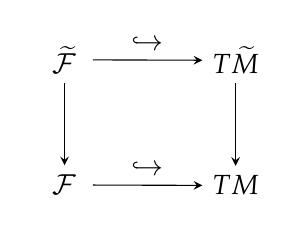
\begin{tikzpicture}
 	\matrix (m) [matrix of math nodes,row sep=3em,column sep=4em,minimum width=2em]
 	{
 		\widetilde{\mathcal F} &    T\widetilde{M} \\
 		\mathcal F	& TM    \\};
 	\path[-stealth]
 	(m-1-1) edge node [above] {$\hookto$} (m-1-2)
 	(m-1-1) edge node [right] {} (m-2-1)
 	(m-1-2) edge node [right] {} (m-2-2)
 	(m-2-1) edge node [above] {$\hookto$}  (m-2-2);
 	
 	\end{tikzpicture}
 	\newline
 	then $\widetilde{\mathcal F}$ is integrable.
 	
 	\begin{definition}\label{fol_cov_defn}
 		In the above situation we say that a foliation $\left(\widetilde{M},~ \widetilde{\mathcal F} \right)$ is the \textit{induced by} $p$ \textit{covering} of $\left(M,\mathcal F \right)$ or the $p$-\textit{lift} of $\left(M,\mathcal F \right)$. 
 	\end{definition}
\begin{remark}
 		The $p$-lift of a foliation is described in  \cite{ouchi:cov_fol, xiaolu:foli_cov}.
 	\end{remark}
 \begin{empt}
 	If $\gamma: \left[0,1\right]\to M$ is a path which corresponds to an element of the holonomy groupoid then we denote by $\left[\gamma\right]$ its equivalence class, i.e. element of groupoid.
 	There is the space of half densities $\Omega_{\widetilde{M}}^{1/2}$ on $\widetilde{M}$ which is a lift  the space of half densities $\Omega_{M}^{1/2}$ on $M$. If $L$ is a leaf of $\left(M,\mathcal F \right)$, $L'=\pi^{-1}\left( L\right)$   then a space $\widetilde{L}$ of holonomy covering of  $L$ coincides with the space of the holonomy covering of $L'$. It turns out that $L^2\left( \widetilde{\mathcal G}_{\widetilde{x}}\right)\approx L^2\left(\mathcal G_{ \pi\left(\widetilde{x}\right)} \right)$ for any $\widetilde{x} \in \widetilde{M}$.
 	If $\mathcal G$ (resp. $\widetilde{\mathcal G}$) is a holonomy groupoid of $\left(M,\mathcal F \right)$ (resp. $\left(\widetilde{M},~ \widetilde{\mathcal F} \right)$) then there is the surjective map $p_{\mathcal G}:\widetilde{\mathcal G} \to \mathcal G$ given by
 	\begin{equation*}
 	\begin{split}
 	\left[\widetilde{\gamma}\right] \mapsto \left[p \circ\widetilde{\gamma}\right]
 	\end{split}
 	\end{equation*}
 	If the covering is finite-fold then the map $p_{\mathcal G}:\widetilde{\mathcal G} \to \mathcal G$ induces 
 	a natural involutive homomorphism
 	\begin{equation*}
 	\begin{split}
 	\Coo_c\left(\mathcal G,  \Omega_{M}^{1/2}\right) \hookto  \Coo_c\left(\widetilde{\mathcal G},  \Omega_{\widetilde{M}}^{1/2}\right)
 	\end{split}
 	\end{equation*}	
 	Completions of $\Coo_c\left(\mathcal G,  \Omega_{M}^{1/2}\right)$ and $\Coo_c\left(\widetilde{\mathcal G},  \Omega_{\widetilde{M}}^{1/2}\right)$ with respect to given by \eqref{fol_norm_eqn} norms gives an injective *- homomorphism 
 	\be\label{foli_inc_eqn}
 	\pi: C^*_r\left( M,\mathcal F\right) \hookto C^*_r\left(\widetilde{M},~ \widetilde{\mathcal F} \right)
 	\ee
 	 of $C^*$-algebras. The action of the group $G\left( \left.\widetilde{M}~\right|M\right)$ of covering transformations on $\widetilde{M}$ naturally induces an action of $G\left( \left.\widetilde{M}~\right|M\right)$ on $\left(\widetilde{M},~ \widetilde{\mathcal F} \right)$.  It follows that there is the natural action   $C^*_r\left(\widetilde{M},~ \widetilde{\mathcal F} \right)$ such that 
 	\be\label{foli_exp_g_eqn}
 	C^*_r\left( M, \mathcal{F}\right)   = C^*_r\left(\widetilde{M},~ \widetilde{\mathcal F} \right)^{G\left( \left.\widetilde{M}~\right|M\right)}
 	\ee
 \end{empt}

 	Let $\G\left({M},~ {\mathcal F} \right)$ and $\G\left(\widetilde{M},~ \widetilde{\mathcal F} \right)$ be the holonomy groupoids of $\left({M},~ {\mathcal F} \right)$ and $\left(\widetilde{M},~ \widetilde{\mathcal F} \right)$ respectively. The natural surjective map $\G\left(\widetilde{M},~ \widetilde{\mathcal F} \right)\to\G\left({M},~ {\mathcal F} \right)$ induces the injective *-homomorphism $C_r^*\left(\widetilde{M},~ \widetilde{\mathcal F} \right)\hookto C^*_r\left(\widetilde{M},~ \widetilde{\mathcal F} \right)$.
 	Assume both $\G\left({M},~ {\mathcal F} \right)$ and $\G\left(\widetilde{M},~ \widetilde{\mathcal F} \right)$ are Hausdorff. Let $G\left( \left.\widetilde{M}~\right|M\right)$  be the covering 	group of  $p:\widetilde M \to M$ . The $G\left( \left.\widetilde{M}~\right|M\right)$-action on $\widetilde{M}$ can be naturally extended to $\G\left(\widetilde{M},~ \widetilde{\mathcal F} \right)$ by sending $\widetilde{\ga}$ to $g\widetilde{\ga}$ for a representative path $\widetilde{\ga}$ in $ \widetilde{M}$ and $g \in G\left( \left.\widetilde{M}~\right|M\right)$. %Therefore we have a transformation groupoid $G\left( \left.\widetilde{M}~\right|M\right)\times \G\left(\widetilde{M},~ \widetilde{\mathcal F} \right)$, with the composition law $\left(g',g\widetilde{\ga} \right)\left(g, \widetilde{\ga}\right) =  \left(g'g, \widetilde{\ga}\right)$.  	 Let $G = \G\left({M},~ {\mathcal F} \right)$, $H = G\left( \left.\widetilde{M}~\right|M\right)\times \G\left(\widetilde{M},~ \widetilde{\mathcal F} \right)$, and $Z = \G\left(\widetilde{M},~ \widetilde{\mathcal F} \right)$. Clearly, the  		unit spaces are $G^0 = M$ and $H^0 = M$. Define $\rho: Z \to G^0$ and $\sigma: Z \to H^0$ by $\rho\left(\widetilde{\ga}\right)= p\left(r\left(\widetilde{\ga} \right)  \right)$  $\sigma\left( \widetilde{\ga}\right) = p\left(r\left( \widetilde{\ga}\right)  \right)$. Both are continuous open maps. The space $Z$ is
 	\begin{lemma}\cite{xiaolu:foli_cov}
 	Let $p:\widetilde M \to M$ be a regular covering manifold with covering group $G\left( \left.\widetilde{M}~\right|M\right)$
 	$N\subset M$ a connected submanifold, and $\widetilde N$ a connected component of $p^{-1}\left( N\right) $
 	Then the restriction $p_{\widetilde N}$ of $p$ to $N$ is also regular, with the covering group $G\left( \left.\widetilde{N}~\right|N\right)$ being a  	subgroup  $G\left( \left.\widetilde{M}~\right|M\right)$.
 	\end{lemma}
 In particular, if $L_{\widetilde x}$ is the leave in $\left(\widetilde{M},~ \widetilde{\mathcal F} \right)$ containing $\widetilde x \in p^{-1}\left( x\right)$ , where $x \in M$,
 then $L_{\widetilde x}$ is a regular cover of $L_x$. We denote the covering group by $G\left( \left.\widetilde{M}~\right|M\right)_x$. On the  other hand, for each $x \in M$, there is a holonomy group $\G^x_x$, and we have the holonomy group bundle $\left\{\G^x_x\right\}$ over $M$. If $x_1$, $x_2$ are on the same leaf, then any path $\ga$  connecting $x_1$ and $x_2$ induces an isomorphism $\ga^*: \G^{x_1}_{x_1}\xrightarrow{\cong}\G^{x_2}_{x_2}$  by mapping $\left[\ga_1\right]$ to $\left[\ga\ga_1\ga^{-1}\right]$.
As a local homeomorphism, the covering map $p$ induces an embedding $\overline{p} : \G^{\widetilde x}_{\widetilde x}\to \G^x_x$ for each $\widetilde x \in p^{-1}\left( x\right)$.
\begin{lemma}\cite{xiaolu:foli_cov}
The group $\overline{p}^*_x\left(\G^{\widetilde x}_{\widetilde x}\right)$ is a normal subgroup of $G^x_x$. Equivalently,
$\overline{p}^*_x\left( \G^{\widetilde x_1}_{\widetilde x_1}\right) =\overline{p}^*_x\left( \G^{\widetilde x_2}_{\widetilde x_2}\right)$ for $\widetilde x_1, \widetilde x_2 \in p^{-1}\left(x\right)$ if $L_{\widetilde x_1}=L_{\widetilde x_2}$,
\end{lemma}
Thus we may form the quotient holonomy group bundle $\left\{\G^{\widetilde x}_{\widetilde x}\right\}$ over $M$. There is an obvious group homomorphism $\phi_x: G\left( \left.\widetilde{M}~\right|M\right)_x \to \G^{ x}_{ x}/\G^{\widetilde x}_{\widetilde x}$ defined as follows. An element $g\in G\left( \left.\widetilde{M}~\right|M\right)_x$ corresponds to a point $x_g \in p^{-1}\left( x\right)\cap L_{\widetilde x}$ if we fix $\widetilde x$ corresponding
to the unit $e$. A path $\ga_g$ starting at  $\widetilde x$ and ending at $g \widetilde x$ gives a loop $\pi\left(\widetilde \ga_g \right)$  in $M$ representing an element $\phi_x\left(g \right)$  in $G_x$, whose class in $\G^{ x}_{ x}/\G^{\widetilde x}_{\widetilde x}$ is uniquely defined
	by $g$. Given any $\left[\ga\right]$ in $\G^{ x}_{ x}$ there is a preimage $\widetilde \ga$ in $L_{\widetilde x}$ starting at $\widetilde x$. The point $r\left( \widetilde \ga\right) \in p^{-1}\left( x\right)\cap  L_{\widetilde x}$ corresponding to some $g\in G\left( \left.\widetilde{M}~\right|M\right)_x$. So $\phi_x$ is onto.
	\begin{definition}\cite{xiaolu:foli_cov}\label{foli_reg_cov_defn}
		The covering map $p:\left(\widetilde{M},~ \widetilde{\mathcal F} \right)\to\left({M},~ {\mathcal F} \right)$ of foliations is said to be \textit{regular} if the map $\phi$ is an isomorphism from the leaf covering group bundle to the quotient holonomy group bundle.
	\end{definition}

\begin{remark}\label{foli_action_rem}
Every regular covering map $p:\left(\widetilde{M},~ \widetilde{\mathcal F} \right)\to\left({M},~ {\mathcal F} \right)$ of foliations induces nontrivial action of $G\left( \left.\widetilde{M}~\right|M\right)$ on $C^*_r\left(\widetilde{M},~ \widetilde{\mathcal F}  \right)$ such that $$C^*_r\left(\widetilde{M},~ \widetilde{\mathcal F}  \right)^{ G\left( \left.\widetilde{M}~\right|M\right)}\cong C^*_r\left(\widetilde{M},~ \widetilde{\mathcal F}  \right).$$
\end{remark}


 	\chapter{Miscellany}
 		\section{Pre-order category}
 	\begin{definition}\label{preordercat_defn}\cite{goldblatt:topoi}
 		A category is said to be a \textit{pre-order category} if there is at most one morphism between different objects.
 	\end{definition}
 	\begin{definition}
 		A binary relation $R \subset \La\times \La$ on the set $\La$ (writing $pRq$ in place of $\left(p,q \right)\in R$ ) is said to be \textit{pre-ordering} if it is 
 		\begin{enumerate}
 			\item [(a)] \textit{reflexive}, i.e. for each $p$ we have $pRp$ and
 			\item[(b)] \textit{transitive}, whenever $pRq$ and $qRs$, we have $pRs$.
 		\end{enumerate}
 	\end{definition}
 	\begin{remark}\label{pre_order_rem}
 		For any set $\La$ with pre-ordering $R$ there is a pre-order category such that
 		\begin{enumerate}
 			\item [(a)] Objects of the category are elements of $\La$.
 			\item[(b)] Morphisms are pairs $\left(p, q \right) \in R$.
 			\item[(c)] The composition of morphisms is given by $\left(q,s\right)\circ \left(p, q\right) =\left(p,s\right)$.
 		\end{enumerate}
 		
 	\end{remark}
 	
 \section{Flat connections in the differential geometry}\label{geom_flat_subsec}
 \paragraph*{}
 Here I follow to \cite{koba_nomi:fgd}. Let $M$ be a manifold and $G$ a Lie group. A (\textit{differentiable}) \textit{principal bundle over M with group} $G$ consists of a manifolfd $P$ and an action of $G$ on $P$ satisfying the following conditions:
 \begin{enumerate}
 	\item [(a)] $G$ acts freely on $P$ on the right: $\left(u, a \right) \in P \times G \mapsto ua = R_au \in P$;
 	\item[(b)] $M$ is the quotient space of $P$ by the equivalence relation induced by $G$, i.e. $M = P/G$, and the canonical projection $\pi: P \to M$ is differentiable;
 	\item[(c)] $P$ is locally trivial, that is, every point $x$ of $M$ has an open neighborhood $U$ such that $\pi^{-1}\left( U\right)$ is isomophic to  $U\times G$ in the sense that there is a diffeomorphism $\psi:  \pi^{-1}\left( U\right) \to U \times G$ such that $\psi\left( u\right) = \left( \pi\left( u\right), \varphi\left(u \right) \right) $ where $\varphi$ is a mapping of $\pi^{-1}\left(U \right)$ into $G$ satisfying  $\psi\left(ua \right)= \left( \psi\left( u\right)\right) a$  for all $u \in \pi^{-1}\left(U \right)$ and $a \in G$. 
 \end{enumerate}
 A principal fibre bundle will be denoted by $P\left( M, G, \pi\right), ~ P\left(M, G \right)$ or simply $P$.
 \paragraph*{} Let $P\left(M, G \right)$ be a principal fibre bundle over a manifold with group $G$. For each $u \in P$ let $T_u\left(P \right)$ be a tangent space of $P$ at $u$ and $G_u$ the subspace of $T_u\left( P\right)$ consisting of vectors tangent to the fibre through $u$. A \textit{connection} $\Ga$   in $P$ is an assignment of a subspace $Q_u$ of $T_u\left(P \right)$ to each $u \in P$ such that
 \begin{enumerate}
 	\item [(a)] $T_u\left(P \right) = G_u \oplus Q_u$ (direct sum);
 	\item[(b)] $Q_{ua}= \left(R_a \right)_*Q_u$ for every $u \in P$ and $a \in G$, where $R_a$ is a transformation of $P$ induced by $a \in G, ~ R_au=ua$.
 \end{enumerate}
 \paragraph*{}
 Let $P = M \times G$ be a trivial principal bundle. For each $a \in G$, the set $M \times \{a\}$ is a submanifold of $P$. The \text{canonical flat connection} in $P$ is defined by taking the tangent space to $M \times \{a\}$ at $u = \left(x, a \right)$ as the horizontal tangent subspace at $u$. A connection in any principal bundle is called \textit{flat} if every point has a neighborhood such that the induced connection in $P|_U = \pi^{-1}\left(U \right)$ is isomorphic with the canonical flat connection.
 \begin{cor}\label{dg_flat_cor}(Corollary II 9.2 \cite{koba_nomi:fgd})
 	Let $\Ga$ be a connection in $P\left(M, G \right)$ such that the curvature vanishes identically. If $M$ is paracompact and simply connected, then $P$ is isomorphic to the trivial bundle and $\Ga$ is isomorphic to the canonical flat connection in $M \times G$.
 \end{cor}
 \paragraph*{}
 
 If $\widetilde{\pi}: \widetilde{M} \to M$ is a covering then the $\widetilde{\pi}$-\textit{lift} of $P$ is a principal $\widetilde{P}\left(\widetilde{M}, G \right)$  bundle, given by
 \be\nonumber
 \widetilde{P} = \left\{\left(u, \widetilde{x}\right) \in P \times \widetilde{M}~|~ \pi\left(u \right) = \widetilde{\pi}\left( \widetilde{x}\right) \right\}.
 \ee
 If $\Ga$ is a  connection on $P\left( M, G\right)$ and $\widetilde{M} \to M$ is a covering then is a canonical connection $\widetilde{\Ga}$ on $\widetilde{P}\left(\widetilde{M}, G \right)$ which is the \textit{lift} of $\Ga$, that is, for any $\widetilde{u} \in \widetilde{P}$ the horizontal space $\widetilde{Q}_{\widetilde{u}}$ is isomorphically  mapped onto the horizontal space $Q_{\widetilde{\pi}\left(\widetilde{u} \right) }$ associated with the connection $\Ga$.
 If $\Ga$ is flat then from the Proposition (II 9.3 \cite{koba_nomi:fgd}) it turns out that there is a covering $\widetilde{M} \to M$ such that $\widetilde{P}\left(\widetilde{M}, G \right)$ (which is the lift of $P\left(M,G\right)$) is a trivial bundle, so the lift $\widetilde{\Ga}$ of $\Ga$ is a canonical flat connection (cf. Corollary \ref{dg_flat_cor}). From the the Proposition (II 9.3 \cite{koba_nomi:fgd}) it follows that for any flat connection $\Ga$  on $P\left(M, G \right)$ there is a group homomorphism $\varphi: G\left( \widetilde{M} ~|~ M\right) \to G$ such that
 \begin{enumerate}
 	\item [(a)] There is an action $G\left( \widetilde{M} ~|~ M\right) \times \widetilde{P} \to \widetilde{P} \approx \widetilde{M} \times G$ given by
 	$$
 	g \left(\widetilde{x}, a \right) = \left( g\widetilde{x}, \varphi\left( g\right) a\right); \forall \widetilde{x} \in \widetilde{M}, ~ a \in G, 
 	$$
 	\item[(b)] There is the canonical diffeomorphism  $P = \widetilde{P}/G\left( \widetilde{M} ~|~ M\right)$,
 	\item[(c)] The lift $\tilde{\Ga}$ of $\Ga$ is a canonical flat connection.
 \end{enumerate}
 
 \begin{defn}
 	In the above situation we say that the flat connection $\Ga$ is \textit{induced} by the covering $\widetilde{M}\to M$ and the homomorphism $G\left( \left.\widetilde{M}~\right|M\right) \to G$, or we say that $\Ga$ \textit{comes from} $G\left( \left.\widetilde{M}~\right|M\right) \to G$.
 \end{defn}
 \begin{remark}
 	The  Proposition (II 9.3 \cite{koba_nomi:fgd}) assumes that $\widetilde{M} \to M$ is the universal covering however it is not always necessary requirement.
 \end{remark}
 \begin{remark}
 	If $\pi_1\left(M, x_0 \right)$ is the fundamental group \cite{spanier:at} then there is the canonical surjective homomorphism $\pi_1\left(M, x_0 \right) \to G\left( \left.\widetilde{M}~\right|M\right)$. So there exist the composition $\pi_1\left(M, x_0 \right) \to G\left( \left.\widetilde{M}~\right|M\right) \to G$. It follows that any flat connection comes from the homomorphisms $\pi_1\left(M, x_0 \right) \to G$. 
 \end{remark} 
 \paragraph*{}
 Suppose that there is the right action of $G$ on $P$ and suppose that $F$ is a manifold with the left action of $G$. There is an action of $G$ on $P \times F$ given by $a\left( u, \xi\right) = \left(u a, a^{-1}\xi \right)$ for any $a \in G$ and $\left( u, \xi\right) \in P\times F$. The quotient space $P \times_G F = \left(P \times F \right)/G$ has the natural structure of a manifold and if $E =  P \times_G F$ then $E\left(M, F, G, P \right)$ is said to be the \textit{fibre bundle over the base $M$, with (standard) fibre $F$, and (structure) group G which is associated with the principal bundle P} (cf. \cite{koba_nomi:fgd}). If $P = M \times G$ is the trivial bundle then $E$ is also trivial, that is, $E = M \times F$. If $F = \C^n$ is a vector space and the action of $G$ on $\C^n$ is a linear representation of the group then $E$ is the linear bundle. Denote by $T\left(M \right)$ (resp. $T^*\left(M \right)$) the tangent  (resp. contangent) bundle, and denote by $\Ga\left( E\right)$, $\Ga\left(T\left(M \right)\right)$, $\Ga\left(T^*\left(M \right)\right)$ the spaces of sections of $E$, $T\left(M \right)$, $T^*\left(M \right)$ respectively. Any connection $\Ga$ on $P$ gives a covariant derivative  on $E$, that is,
 for any section  $X \in \Ga\left( T\left(M \right)\right) $ and any section $\xi \in \Ga\left( E\right)$ there is the derivative given by
 \be\nonumber
 \nabla_X\left( \xi\right) \in \Ga\left( E\right).
 \ee
 If $E = M \times \C^n$, $\Ga$ is the canonical flat connection and $\xi$ is a trivial section, that is, $\xi = M \times \{x\}$ then 
 \be\label{comm_triv_eqn}
 \nabla_X \xi = 0,~~ \forall X \in T\left(M \right).
 \ee
 For any connection there is the unique map
 \be\label{comm_alg_conn}
 \nabla : \Ga\left( E\right) \to \Ga\left( E \otimes T^*\left( M\right) \right)
 \ee
 such that
 \be\nonumber
 \nabla_X \xi = \left(\nabla \xi, X \right)
 \ee
 where the pairing $\left(\cdot, \cdot\right) : \Ga\left( E \otimes T^*\left( M\right) \right) \times \Ga\left( T\left( M\right)\right)  \to \Ga\left( E \right) $ is induced by the pairing $\Ga\left( T^*\left(M \right)\right)   \times \Ga\left( T\left( M\right)\right)  \to \Coo\left(M \right) $.
 
 \section{Quantum $SU\left(2 \right)$ and $SO\left(3 \right)$}
 \paragraph*{}
 There is a quantum generalization of $SU\left(2 \right)$ and  we will introduce a quantum analog of $SO\left(3 \right)$.
 Let $q$ be a real number such that $0<q<1$. 
 A quantum group $C\left( \SU_q(2)\right) $ is the universal $C^*$-algebra algebra generated by two elements $\al$ and $\beta$ satisfying the following relations:
 \begin{equation}\label{su_q_2_rel_eqn}
 \begin{split}
 \al^*\al + \beta^*\beta = 1, ~~ \al\al^* + q^2\beta\beta^* =1,
 \\
 \al\bt - q \bt\al = 0, ~~\al\bt^*-q\bt^*\al = 0,
 \\
 \bt^*\bt = \bt\bt^*.
 \end{split}
 \end{equation}
 From  $C\left( SU_1\left(2 \right)\right) \approx C\left(SU\left(2 \right)  \right)$ it follows that  $C\left( \SU_q(2)\right) $ can be regarded as a noncommutative deformation of the space $SU(2)$. 
 The dense pre-$C^*$-algebra $\Coo\left( SU_q(2)\right) \subset C\left( SU_q(2)\right)$ is defined in  \cite{chakraborty_pal:quantum_su_2}. 
 Let $Q, S \in B\left( \ell_2\left(\N^0 \right)\right) $ be given by 
 \begin{equation*}
 \begin{split}
 Qe_k= q^ke_k, \\
 Se_k = \left\{
 \begin{array}{c l}
 e_{k-1} & k > 0 \\
 0 & k = 0
 \end{array}\right..
 \end{split}
 \end{equation*}
 and let $R \in B\left( \ell_2\left(\Z \right)\right) $ be given by $e_k \mapsto e_{k+1}$.
 There is a faithful representation \cite{woronowicz:su2}  $C\left(\SU_q\left( 2\right) \right) \to B\left(\ell_2\left(\N^0 \right) \otimes \ell_2\left(\Z \right) \right)  $ given by
 
 \begin{equation}\label{su_q_2_repr_eqn}
 \begin{split}
 \al \mapsto S\sqrt{1 - Q^2} \otimes 1, \\
 \bt \mapsto Q \otimes R.
 \end{split}
 \end{equation}
  There is a faithful state $h:C\left( SU_q(2)\right) \to \C$ given by
 \be\label{su_q_2_haar_eqn}
 h\left(a \right)  = \sum_{n = 0}^\infty q^{2n}\left(e_n \otimes e_0, a  e_n \otimes e_0\right) 
 \ee
 where $a \in C\left( SU_q(2)\right)$ and $e_0 \otimes e_n \in \ell_2\left(\N^0 \right) \otimes \ell_2\left(\Z \right)$ (cf. \cite{woronowicz:su2}).
 \begin{defn}
 	The state $h$ is said to be the \textit{Haar measure}.
 \end{defn}
 
 Denote by $L^2\left( C\left( SU_q\left(2\right)\right), h\right) $ the GNS space associated with the state $h$. 
 The representation theory of $SU_q(2)$ is strikingly similar to its
 classical counterpart.  In particular, for each $l\in\{0,\frac{1}{2},
 1,\ldots\}$, there is a unique irreducible unitary representation
 $t^{(l)}$ of dimension $2n+1$.  Denote by $t^{(l)}_{jk}$ the
 $jk$\raisebox{.4ex}{th} entry of $t^{(l)}$. These are all elements of
 $\A_f$ and they form an orthogonal basis for $L^2\left( C\left( SU_q\left(2\right)\right), h\right)$. Denote by
 $e^{(l)}_{jk}$ the normalized $t^{(l)}_{jk}$'s, so that
 $\{e^{(l)}_{jk}: n=0,\frac{1}{2},1,\ldots, i,j=-n,-n+1,\ldots, n\}$ is
 an orthonormal basis. The definition of equivariant operators (with respect to action of quantum groups) is described in \cite{chakraborty_pal:inv_hom}. It is proven in \cite{chakraborty_pal:quantum_su_2} that any unbounded equivariant operator $\widetilde{D}$ satisfies to the following condition
 \be \label{su_q_2_dirac_eqn}
 \widetilde{D}: e^{(l)}_{jk}\mapsto d(l,j)e^{(l)}_{jk},
 \ee
 Moreover if
 \be \label{su_q_2_genericd_eqn}
 d(l,j)=\begin{cases}2l+1 &  l \neq j,\cr
 	-(2l+1) & l=j,\end{cases}
 \ee
 
 then there is a 3-summable spectral triple 
 \be \label{su_q_2_spt_eqn}
 \left(\Coo\left( SU_q\left(2\right)\right), L^2\left( C\left( SU_q\left(2\right)\right), h\right), \widetilde{D} \right) 
 \ee
 described in \cite{chakraborty_pal:quantum_su_2}. 
 
 According to \cite{kl-sch} (equations (4.40)-(4.44) ) following condition holds
 \begin{equation}\label{su_q_2_tij_eqn}
 \begin{split}
 t^{\left(l \right) }_{jk}= M^l_{jk} \al^{-j-k}\bt^{k-j}p_{l + k}\left( \bt\bt^*; q^{-2\left(k-j \right) }q^{2\left(j + k \right)}~|~q^2 \right); ~~ j + k \le 0 ~\&~ k \ge j,
 \\ 
 t^{\left(l \right) }_{jk}= M^l_{jk} \al^{-j-k}\bt^{*\left( k-j\right) }p_{l + k}\left( \bt\bt^*; q^{-2\left(k-j \right) }q^{2\left(j + k \right)}~|~q^2 \right); ~~ j + k \le 0 ~\&~ k \le j,
\\ 
 t^{\left(l \right) }_{jk}= M^l_{j,k}p_{l - k}\left( \bt\bt^*; q^{-2\left(k-j \right) }q^{2\left(j + k \right)}~|~q^2 \right)\bt^{k-j}\al^{*j+k}; ~~ j + k \ge 0 ~\&~ k \ge j,\\ 
 t^{\left(l \right) }_{jk}= M^l_{k,j}p_{l - j}\left( \bt\bt^*; q^{-2\left(k-j \right) }q^{2\left(j + k \right)}~|~q^2 \right)\bt^{*j-k}\al^{*j + k}; ~~ j + k \ge 0 ~\&~ j \ge k\\ 
 \end{split}
 \end{equation}
  where $M^l_{jk} \in \R$ for any $l, j, k$ and $p_{l - k}\left( x; q^{-2\left(k-j \right) }q^{2\left(j + k \right)}~|~q^2 \right)$ is little Jacobi polynomial (cf. \cite{kl-sch}).  
 Denote by $g \in \Z_2$ the unique nontrivial element.
 There is a surjective group homomorphism
 $$
 \Phi : SU\left(2 \right) \to SO\left(3 \right) ,~ \ker \Phi = \Z_2 = \{\pm 1\}
 $$
 and the natural action of $\Z_2$ on $SU(2)$ such that
 \be\label{su_q_2_z2_comm_eqn}
 \begin{split}
 	SO\left(3 \right) \cong SU\left(2\right)/\Z_2,\\
 	g\begin{pmatrix} \al & -\overline{\bt}\\
 		\bt & \overline{\al}\end{pmatrix}= \begin{pmatrix} -\al & \overline{\bt}\\
 		-\bt & -\overline{\al}\end{pmatrix};~ \forall \begin{pmatrix} \al & -\overline{\bt}\\
 		\bt & \overline{\al}\end{pmatrix}\in SU\left(2\right).
 \end{split}
 \ee	
 This action induces an action of $\Z_2$  on a $C^*$-algebra $C\left(SU\left(2\right) \right)$ given by
 \be\nonumber
 \begin{split}
 	g\al = -\al, ~~ g\bt = - \bt
 \end{split}
 \ee
 where $\al, \bt$ are regarded as functions $\SU\left(2 \right) \to \C$.
 Indeed 	$ SU\left(2 \right)$ is an oriented manifold, $SO\left(3 \right)$ is an unoriented one, and $ SU\left(2 \right) \to SO\left(3 \right)$ is a two-fold covering
 There is a quantum generalization of $SU\left(2 \right)$ and  we will introduce a quantum analog of $SO\left(3 \right)$.
 Let $q$ be a real number such that $0<q<1$. 
There is a noncommutative analog of the action \eqref{su_q_2_z2_comm_eqn} described in \cite{dijkhuizen:so_doublecov,lance:so,podles:so_su}
\begin{equation}\label{su_q_2_z2_ncomm_eqn}
\begin{split}
\Z_2 \times C\left( SU_q\left(2\right)\right)\to C\left( SU_q\left(2\right)\right),\\
g\al = -\al,~g \bt = -\bt.
\end{split}
\end{equation} 
In \cite{dijkhuizen:so_doublecov,lance:so,podles:so_su} the quantum group 	$SO_q\left(3 \right)$ is defined, moreover in 
it is proven in \cite{dijkhuizen:so_doublecov,podles:so_su} following 
$$
	C\left( 	SO_q\left(3 \right) \right) \stackrel{\mathrm{def}}{=} C\left( SU_q\left(2\right)\right) ^{\Z_2}\cong \left\{\widetilde{a}\in C\left( SU_q\left(2\right)\right) ,~ g\widetilde{a} = \widetilde{a} \right\}.
$$
Above equation can be used as the definition of $SO_q\left(3 \right)$
 \begin{definition}\label{su_q_2_so3_defn}
	Denote by
	\begin{equation}\label{su_q_2_so3_eqn}
	C\left( 	SO_q\left(3 \right) \right) \stackrel{\mathrm{def}}{=} C\left( SU_q\left(2\right)\right) ^{\Z_2}\cong \left\{\widetilde{a}\in C\left( SU_q\left(2\right)\right) ,~ g\widetilde{a} = \widetilde{a} \right\}.
	\end{equation}
	The $C^*$-algebra $C\left( 	SO_q\left(3 \right)\right) $ is said to be the \textit{quantum 	$ SO\left(3 \right)$}.
\end{definition}
\begin{remark}
	Our definition of $SO_q\left(3 \right)$  differs from the Definition given in other sources. For example the quantum group defined in \cite{rtf:qlie} is a
	quantization of $O\left( 3\right)$  and not of $SO(3)$ (cf. \cite{dijkhuizen:so_doublecov}). 
\end{remark}

 \begin{thm}\label{su_q_2_bas_thm}\cite{woronowicz:su2}
 	Let  $q \neq 0$, and let $\A_f$ the dense involutive subalgebra of $C\left( SU_q(2)\right)$ generated  by $\alpha, \beta$. The set of elements of the form
 	\be\label{su_q_2_fin_eqn}
 	\al^k\bt^n\bt^{*m}~~ \text{ and }~~ \al^{*k'}\bt^n\bt^{*m}
 	\ee 
 	where $k, m, n = 0, \dots;~k'=1, 2,\dots$ forms a basis in $\A_f$: any element
 	of $\A_f$ can be written in the unique way as a finite linear combination of
 	elements of \eqref{su_q_2_fin_eqn}.
 \end{thm}
\section{Presheaves and Sheaves}

\begin{definition}\label{presheaf_defn}\cite{hartshorne:ag}
Let $\sX$ be a topological space. A \textit{presheaf} $\mathscr F$ of Abelian groups on  $\sX$ consists of the data
\begin{itemize}
	\item[(a)] for every open subset $\sU \subseteq \sX$, an Abelian group $\mathscr F\left(\sU\right)$, and 
	\item[(b)] for every inclusion $\sV \subseteq \sU$ of open subsets of $\sX$, a morphism of Abelian groups $\rho_{\sU \sV}:\mathscr F\left(\sU\right) \to \mathscr F\left(\sV\right)$,\\
	subject to conditions
	\begin{itemize}
		\item [(0)] $\mathscr F\left(\sV\right)= 0$, where $\emptyset$ is the empty set,
		\item[(1)] $\rho_{\sU \sU}$ is the identity map, and
		\item[(2)] if $\mathcal W \subseteq \sV \subseteq \sU$ are three open sets, then $\rho_{\sU \mathcal W} = \rho_{\sV \mathcal W }\circ \rho_{\sU \sV}$.
	\end{itemize}
\end{itemize}
\end{definition}

\begin{definition}\label{sheaf_defn}\cite{hartshorne:ag}
	 A \textit{presheaf} $\mathscr F$ on a 
 a topological space $\sX$ is a \textit{presheaf} $\mathscr F$ if it satisfies the following supplementary conditions:
	\begin{itemize}
		\item[(3)] If $\sU$ is an open set, if $\left\{\sV_{\a}\right\}$ is an open covering of $\sU$, and if $s \in \mathscr F\left(\sU\right)$ is an element such that $\left.s\right|_{\sV_{\a}}= 0$ for all $\a$, then $s = 0$;
		\item[(4)] If $\sU$ is an open set, if $\left\{\sV_{\a}\right\}$ is an open covering of $\sU$, and we have elements $s_\a$ for each $\a$, with property that for each $\al, \bt, \left.s_\a\right|_{\sV_{\a}\cap \sV_{\bt}}= \left.s_\a\right|_{\sV_{\bt}\cap \sV_{\bt}}$, then there is an element $s \in  F\left(\sV\right)$ such that $\left.s\right|_{\sV_\a} = s_\a$ for each $\a$.
	\end{itemize}
(Note condition (3) implies that $s$ is unique.)
\end{definition}
\begin{definition}
	A presheaf satisfying (4) of the Definition \ref{sheaf_defn} is called \textit{conjunctive} (for $\sU$). (cf. \cite{bredon:sheaf})
\end{definition}

\begin{definition}\label{stalk_defn}\cite{hartshorne:ag}
	If $\mathscr F$ is a {presheaf} on $\sX$, and if $x$ is a point of $\sX$ we define the \textit{stalk} $\mathscr F_x$ of $\mathscr F$ at $x$ to be the direct limit of groups $\mathscr F\left(\sU\right)$ for all open sets $\sU$ containing $x$, via restriction maps $\rho$.
	\end{definition}

\begin{prdf}\label{sheaf_prdf}\cite{hartshorne:ag}
	Given a presheaf $\mathscr F$, there is a sheaf $\mathscr F^+$ and a morphism $\th: \mathscr F \to \mathscr F^+$, with the property that for any sheaf $\mathscr G$, and any morphism $\varphi: \mathscr F \to \mathscr G$, there is a unique morphism $\psi:\mathscr F^+\to \mathscr G$ such that $\varphi = \psi \circ \th$. Furthermore the pair $\left(\mathscr F^+, \th\right)$ is unique up to unique isomorphism. $\mathscr F^+$ is called the $\mathrm{sheaf~associated}$ to the preseaf $\mathscr F$. 
\end{prdf}
\begin{empt}\label{sheaf_empt}
Following text is the citation of the proof of \ref{sheaf_prdf} (cf. \cite{hartshorne:ag}). For any open set $\sU$, let $\mathscr F^+\left(\sU\right)$ be set of functions $s$ from $\sU$ to the union $\bigcup_{x \in \sU}  \mathscr F_x$ of stalks of $\mathscr F$ over points of $\sU$, such that
\begin{itemize}
	\item [(1)] for each $x \in \sU$, $s\left(x\right)\in \mathscr F_x$, and
	\item[(2)] for each $x \in \sU$, there is a neighborhood $\sV$ of $x$ contained in $\sU$ and an element $t \in \mathscr F\left(\sV\right)$, such that for all $y \in \sV$ the germ $t_y$ of $t$ at $y$ is equal to $s\left(y\right)$.
\end{itemize}
\end{empt}
\begin{definition}\label{sheaf_inv_im_defn}\cite{hartshorne:ag}
	Let $f: \sX\to \sY$ be a continuous map of topological spaces. For any sheaf $\mathscr F$ on $\sX$, we define the \textit{direct image} sheaf $f_*\mathscr F$ on $\sY$ by $\left(f_*\mathscr F\right)\left(\sV\right)= \mathscr F\left(f^{-1}\left(\sV\right)\right)$ for any open set $\sV \subseteq \sV$. For any sheaf $\mathscr G$ on $\sY$, we define the \textit{inverse image} sheaf $f^{-1}\mathscr G$ on $\sX$ be the sheaf associated to the presheaf $\sU \mapsto \lim_{\sV \supseteq f\left(\sU\right)} \mathscr G\left(\sV\right)$, where $\sU$ is any open set in $\sX$, and the limit is taken over all open sets $\sV$ of $\sV$ containing $f\left(\sU\right)$.
\end{definition}
\begin{empt}\label{sheaf_hom_defn}\cite{hartshorne:ag}
	Let $\mathscr F$, $\mathscr G$ be sheaves of Abelian  groups  on $\sX$. For any open set $\sU \subseteq \sX$ the set of morphisms $\Hom\left(\left.\mathscr F\right|_{\sU}, \left.\mathscr G\right|_{\sU}\right)$ has the natural structure of Abelian group. It is a sheaf (cf. \cite{hartshorne:ag}). It is called the \textit{sheaf of local morphisms} of $\mathscr F\to \mathscr G$, "sheaf hom" for short, and is denoted by $\mathscr Hom \left(\mathscr F, \mathscr G\right)$.
\end{empt}

\begin{definition}\label{sheaf_flasque}\cite{hartshorne:ag}
A sheaf $\mathscr F$ on a topological space is \textit{flasque} or \textit{flabby} if for every inclusion $\sV \subseteq \sU$ of open sets, the restriction map $\mathscr F\left(\sU \right)\to\mathscr F\left(\sV \right)$ is surjective. 
\end{definition}
Recall that for $s \in \mathscr{F}\left(\sX \right)$, $\supp s= \left\{\left.x \in \sX \right|s\left(x \right)\neq 0  \right\}$ denotes the \textit{support} of the section $s$.
\begin{definition}\label{phi_supp_defn}\cite{godement:sheaf}.
Let $\sX$ be a topological space. A \textit{family of supports} on $\sX$ is a family $\Phi$ of closed
subsets of $\sX$  such that:
\begin{enumerate}
	\item a closed subset of a member of $\Phi$ is a member of $\Phi$;
	\item $\Phi$ is closed under finite unions.
\end{enumerate}

$\Phi$  is said to be a  \textit{paracompactifying} family of supports if in addition:
\begin{enumerate}
	\item  each element of $\Phi$ is paracompact;
	\item each element of $\Phi$ has a (closed) neighborhood which is in $\Phi$.
\end{enumerate}
\end{definition}

\begin{definition}
A sheaf $\mathscr{F}$ on $\sX$ is called $\Phi$-\textit{soft} if the restriction map
$\mathscr{F}\left(\sX \right) \to  \mathscr{F}\left(K \right)$  is surjective for all $K \in \Phi$. If $\Phi$ is a set of all closed sets  then $\Phi$ is simply
called \textit{soft}.
\end{definition}
The family of all compact subsets of $\sX$ is denoted by $c$.
 Now is $\mathscr P$ is a presheaf on $\sX$ such and $s \in \mathscr P\left(\sX \right)$ we put
$\left|s\right| = \left|\th\left( s\right) \right|$, where $\th: \mathscr{P}\left(\sX \right)\to \mathscr{P}^+\left(\sX \right) $ is the canonical map, $\mathscr{P}^+$ being the sheaf generated by $\mathscr{P}$.
Note that for $s \in \mathscr{P}$ one has $x \notin \left|s\right|\Leftrightarrow\left.s \right|_{\sU}$ for some neighborhood $\sU$ of $x$. If $\mathscr{F}$ is a sheaf, we put
$$
\Ga_\Phi = \left\{\left.s\in \mathscr{F}\left( \sX\right)\right| \left|s\right| \in \Phi \right\}
$$
For a presheaf $\mathscr{P}$  on $\sX$ we put  $\mathscr{P}_\Phi\left(\sX \right) = \left\{\left.s\in \mathscr{P}\left( \sX\right)\right| \left|s\right| \in \Phi \right\}$.
\begin{lemma}\label{schv_soft_n_lem}\cite{godement:sheaf,torsten:sheaves}
Let $\sX$ be a paracompact space, $\mathscr{F}$ a sheaf on $\sX$. Then $\mathscr{F}$ is soft if and only if every point $x \in \sX$ has a closed neighborhood $\overline{   \mathcal U }$ such that $\left.\mathscr{F}\right|_{\overline{   \mathcal U }}$ is soft.
\end{lemma}
\begin{proposition}\label{flabby_soft_prop}\cite{bredon:sheaf}
	9.22. Proposition. \\
	If $\sU$ is a compact relatively Hausdorff subspace of $\sX$,
	then $\left.\mathscr{F}\right|_{\sU} $ is soft for any flabby sheaf $\mathscr{F}$ on $\sX$.
\end{proposition}


\begin{theorem}
	6.2.\\
Theorem. Let $\mathscr P$ be a presheaf on $\sX$ that is conjunctive for coverings
of $\sX$ and $\mathscr P^+$ be the sheaf generated by $\mathscr P$. Then for any paracompactifying
family $\Phi$ of supports on $\sX$, the sequence
$$
0 \to \mathscr P_0\left( \right) \to  \mathscr{P}_\Phi\left(\sX \right) \xrightarrow{\th}\Ga_\Phi\left(\mathscr{P}^+ \right) 
$$
is exact.
\end{theorem}
\begin{theorem}\label{sheaf_neigh_thm}\cite{godement:sheaf}
	3.3.1\\
Let $\mathscr{F}$ be a sheaf of set over the space $\sX$, $\mathcal S$ is a subset of $\sX$ and $s$ is a section of the sheaf $\mathscr{F}$ over $\mathcal S$. If $\mathcal S$ allows a fundamental system of paracompact neighborhoods then $s$ can be extended to a neighborhood of $\mathcal S$ in $\sX$. 
\end{theorem}
\subsection{Sheaves over non Hausdorff spaces}
\begin{empt}\label{nh_csoft_empt}\cite{cra_moe:nhaus}
Here we assume that the space $\sX$ has an open cover by subsets $\sU \subset \sU$ which are each paracompact, Hausdorff, locally compact and of cohomological dimension bounded a number $d$ (depending  on $\sX$ but not $\sU$).	
\end{empt}

\begin{definition}\label{nh_csoft_defn}\cite{cra_moe:nhaus}
Let $\sX$ be a space satisfying the assumptions of \ref{nh_csoft_empt}. An Abelian sheaf $\mathscr{F}$ is said to be $c$-\textit{soft} if for any open $\sU \subset \sX$ its restriction $\left.\mathscr{F}\right|_{\sU}$ is a $c$-soft on $\sU$ in the usual sense. By the same proprety of for Hausdorff space, it follows that $c$-softness is a local property, i.e. a sheaf  $\mathscr{F}$ is $c$-soft if and only if there is an open cover $\sX= \cup \sU_\a$  such that $\left.\mathscr{F}\right|_{\sU_\a}$ is a $c$-soft sheaf on $\sU$.
\end{definition}
\begin{definition}\label{nh_csoft_gc_defn}\cite{cra_moe:nhaus}
	Let $\mathscr{F}$ be a $c$-soft sheaf and let $\mathscr{F}'$  be its Godement resolution (i.e. $\mathscr{F}'= \Ga\left(\sU_{\text{distr}}, \mathscr{F} \right)$ is the set of all (not necessary continuous) sections for any open $\sU \subset \sX$). For any Hausdorff open set $\mathcal W$, let $\Ga_c\left(\mathcal W, \mathscr{F} \right)$ be the usual set of compactly supported sections. If $\mathcal W \subset \sU$, there is an evident homomorphism "extension by 0" $\Ga_c\left(\mathcal W, \mathscr{F} \right) \hookto \Ga_c\left(\mathcal U, \mathscr{F} \right)\subset \Ga_c\left(\mathcal U, \mathscr{F}' \right)$. For any (not necessary Hausdorff) open set $\sU \subset \sX$ we define $\Ga_c \left(\sU, \mathscr{F} \right)$ to be the image of the map:
	$$
	\bigoplus_{\mathcal W} \Ga_c\left(\mathcal W, \mathscr{F}' \right) \hookto \Ga\left(\mathcal U, \mathscr{F}' \right),
	$$ 
	where $\mathcal W$ ranges over all open subsets $\mathcal W \subset \mathcal U$. %An alternative definition follows by choosing open cover in Propositions \ref{nh_csoft_gc_prop} below.
\end{definition}
\begin{proposition}\label{nh_csoft_gc_lem}
	Let  $\mathscr{F}$ be a $c$-soft sheaf. For any open cover $\sU = \cup \mathcal W_\a$ where each $\mathcal W_\a$ is Hausdorff the sequence $\oplus_\a \Ga_c\left(\mathcal W_\a,  \mathscr{F}\right) \to \Ga_c\left(\mathcal U,  \mathscr{F}\right)\to 0$ is exact.  
\end{proposition}
\section{Isospectral deformations}
\paragraph*{}A very general construction of isospectral
deformations
of noncommutative geometries is described in \cite{connes_landi:isospectral}. The construction
implies in particular that any
compact Spin-manifold $M$ whose isometry group has rank
$\geq 2$ admits a
natural one-parameter isospectral deformation to noncommutative geometries
$M_\theta$.
We let $(\Coo\left(M \right)  , \H = L^2\left(M,S \right)  , \slashed D)$ be the canonical spectral triple associated with a
compact spin-manifold $M$. We recall that $\mathcal{A} = C^\infty(M)$ is
the algebra of smooth
functions on $M$, $S$ is the spinor bundle and $\slashed D$
is the Dirac operator.
Let us assume that the group $\mathrm{Isom}(M)$ of isometries of $M$ has rank
$r\geq2$.
Then, we have an inclusion
\begin{equation}\label{isos_t_act_eqn}
\mathbb{T}^2 \subset \mathrm{Isom}(M) \, ,
\end{equation}
with $\mathbb{T}^2 = \mathbb{R}^2 / 2 \pi \mathbb{Z}^2$ the usual torus, and we let $U(s) , s \in
\mathbb{T}^2$, be
the corresponding unitary operators in $\H = L^2(M,S)$ so that by construction
\begin{equation*}
U(s) \, \slashed D = \slashed D \, U(s).
\end{equation*}
Also,
\begin{equation}\label{isospectral_sym_eqn}
U(s) \, a \, U(s)^{-1} = \alpha_s(a) \, , \, \, \, \forall \, a \in \mathcal{A} \, ,
\end{equation}
where $\alpha_s \in \mathrm{Aut}(\mathcal{A})$ is the action by isometries on the
algebra of functions on
$M$.

\noindent
We let $p = (p_1, p_2)$ be the generator of the two-parameters group $U(s)$
so that
\begin{equation*}
U(s) = \exp(i(s_1 p_1 + s_2 p_2)) \, .
\end{equation*}
The operators $p_1$ and $p_2$ commute with $D$.
Both $p_1$ and $p_2$
have integral spectrum,
\begin{equation*}
\mathrm{Spec}(p_j) \subset \mathbb{Z} \, , \, \, j = 1, 2 \, .
\end{equation*}

\noindent
One defines a bigrading of the algebra of bounded operators in $\H$ with the
operator $T$ declared to be of bidegree
$(n_1,n_2)$ when,
\begin{equation*}
\alpha_s(T) = \exp(i(s_1 n_1 + s_2 n_2)) \, T \, , \, \, \, \forall \, s \in
\mathbb{T}^2 \, ,
\end{equation*}
where $\alpha_s(T) = U(s) \, T \, U(s)^{-1}$ as in \eqref{isospectral_sym_eqn}.
\paragraph{}
Any operator $T$ of class $C^\infty$ relative to $\alpha_s$ (i. e. such that
the map $s \rightarrow \alpha_s(T) $ is of class $C^\infty$ for the
norm topology) can be uniquely
written as a doubly infinite
norm convergent sum of homogeneous elements,
\begin{equation*}
T = \sum_{n_1,n_2} \, \widehat{T}_{n_1,n_2} \, ,
\end{equation*}
with $\widehat{T}_{n_1,n_2}$ of bidegree $(n_1,n_2)$ and where the sequence
of norms $||
\widehat{T}_{n_1,n_2} ||$ is of
rapid decay in $(n_1,n_2)$.
Let $\lambda = \exp(2 \pi i \theta)$. For any operator $T$ in $\H$ of
class $C^\infty$ we define
its left twist $l(T)$ by
\begin{equation}\label{l_defn}
l(T) = \sum_{n_1,n_2} \, \widehat{T}_{n_1,n_2} \, \lambda^{n_2 p_1} \, ,
\end{equation}
and its right twist $r(T)$ by
\begin{equation*}
r(T) = \sum_{n_1,n_2} \, \widehat{T}_{n_1,n_2} \, \lambda^{n_1 p_2} \, ,
\end{equation*}
Since $|\lambda | = 1$ and $p_1$, $p_2$ are self-adjoint, both series
converge in norm. Denote by $\Coo\left(M \right)_{n_1, n_2} \subset \Coo\left(M \right) $ the $\C$-linear subspace of elements of bidegree $\left( n_1, n_2\right) $. \\
One has,
\begin{lem}\label{conn_landi_iso_lem}\cite{connes_landi:isospectral}
	\begin{itemize}
		\item[{\rm a)}] Let $x$ be a homogeneous operator of bidegree $(n_1,n_2)$
		and $y$ be
		a homogeneous operator of  bidegree $(n'_1,n'_2)$. Then,
		\begin{equation}
		l(x) \, r(y) \, - \,  r(y) \, l(x) = (x \, y \, - y \, x) \,
		\lambda^{n'_1 n_2} \lambda^{n_2 p_1 + n'_1 p_2}
		\end{equation}
		In particular, $[l(x), r(y)] = 0$ if $[x, y] = 0$.
		\item[{\rm b)}] Let $x$ and $y$ be homogeneous operators as before and
		define
		\begin{equation*}
		x * y = \lambda^{n'_1 n_2} \, x y \, ; \label{star}
		\end{equation*}
		then $l(x) l(y) = l(x * y)$.
	\end{itemize}
\end{lem}



\noindent
The product $*$ defined in (\ref{star}) extends by linearity
to an associative product on the linear space of smooth operators and could
be called a $*$-product.
One could also define a deformed `right product'. If $x$ is homogeneous of
bidegree
$(n_1,n_2)$ and $y$ is homogeneous of bidegree $(n'_1,n'_2)$ the product is
defined by
\begin{equation*}
x *_{r} y = \lambda^{n_1 n'_2} \, x y \, .
\end{equation*}
Then, along the lines of the previous lemma one shows that $r(x) r(y) = r(x
*_{r} y)$.

We can now define a new spectral triple where both $\H$ and the operator
$\slashed D$ are unchanged while the
algebra $\Coo\left(M \right)$  is modified to $l(\Coo\left(M \right))$ . By
Lemma~{\ref{conn_landi_iso_lem}}~b) one checks that  $l\left( \Coo\left(M \right)\right) $ is still an algebra. Since $\slashed D$ is of bidegree $(0,0)$ one has,
\begin{equation}\label{isospectral_ld_eqn}
[\slashed D, \, l(a) ] = l([\slashed D, \, a]) 
\end{equation}
which is enough to check that $[\slashed D, x]$ is bounded for any $x \in l(\mathcal{A})$. There is a spectral triple $\left(l\left( \Coo\left(M \right)\right) , \H, \slashed D\right)$.
\paragraph{} Denote by $\Coo\left( M_\th\right)$ (resp.  $C\left(M_\th \right)$) the algebra $l\Coo\left( M\right)$ (resp. the operator norm completion of $l\left(\Coo\left( M\right)  \right)  $). Denote by $\rho: C\left(M\right) \to L^2\left( M, S\right) $ (resp. $\pi_\th: C\left(M_\th\right) \to B\left( L^2\left( M, S\right)\right) $ ) natural representations.
%\begin{rem}\label{isosp_grad_rem}
%Indeed there $l: \Coo\left( M\right)  \to \Coo\left( M_{\la}\right) $ is a $\C$-linear isomorphism. The bigrading on $\Coo\left( M\right)$ induces the bigrading $\Coo\left( M_{\la}\right)$.
%\end{rem}
%\begin{empt}
%Denote by $\Ga^\infty\left( M, S\right)$ the space of smooth sections of $S$. Since $M$ is compact any smooth section is square integrable, i.e.
%$$
%\Ga^\infty\left( M, S\right) \subset L^2\left( M, S\right)
%$$ 
%\end{empt}
%and above inclusion is dense. On the other hand for any $n_1, n_2 \in \N$ there is a homogeneous subspace $\Ga^\infty\left( M, S\right)_{n_1,n_2} \subset \Ga^\infty\left( M, S\right)$ given by
%$$
%\Ga^\infty\left( M, S\right)_{n_1,n_2}\left\{\xi \in \Ga^\infty\left( M, S\right)~|~\al_s\left( \xi\right)\exp(i(s_1 n_1 + s_2 n_2))\xi \right\}
%$$
% algebraic direct sum
%$$
%\bigoplus_{n_1,n_1 \in \N } \Ga^\infty\left( M, S\right)_{n_1,n_2}
%$$
%is dense in $L^2\left( M, S\right)$. Otherwise
%$$
%\Coo\left( M\right)_{n'_1,n'_2} \Ga^\infty\left( M, S\right)_{n_1,n_2}\subset \Ga^\infty\left( M, S\right)_{n'_1+n_1,n'_2 + n_2}.
%$$
%From the Remark \ref{isosp_grad_rem} it follows that there is the natural bigrading on $\Coo\left( M_{\la}\right)$. From above construction it turns out
%$$
%\Coo\left( M_{\la}\right)_{n'_1,n'_2} \Ga^\infty\left( M, S\right)_{n_1,n_2}\subset \Ga^\infty\left( M, S\right)_{n'_1+n_1,n'_2 + n_2}.
%$$
%The algebraical direct sum $\bigoplus_{n_1,n_2 \in \N } \Ga^\infty\left( M, S\right)_{n_1,n_2}$ (resp. $\bigoplus_{n_1,n_2 \in \N } \Coo\left( M\right)_{n_1,n_2}$ ) is dense in $L^2\left( M, S\right)$ (resp. $ C\left( M_{\la}\right)$). So the action on $ C\left( M_{\la}\right) \times L^2\left( M, S\right) \to L^2\left( M, S\right)$ can be uniquely defined by the actions of $\Coo\left( M_{\la}\right)_{n'_1,n'_2}$ on $\Ga^\infty\left( M, S\right)_{n_1,n_2}$ for any $n'_1,n'_2, n_1,n_2 \in \N$. 
There is an oriented twisted spectral triple 
\be\label{isos_twisetd_eqn}
\left(l\left( \Coo\left(M \right)\right) , \H, \slashed D\right).
\ee
described in \cite{connes_landi:isospectral}.





 \end{appendices}
 
\begin{thebibliography}{10}
	
	

	\bibitem{apt_mult}	Charles A. Akemann, Gert K. Pedersen, Jun Tomiyama. \textit{Multipliers of $C^*$-algeeas}. Journal of Functional Analysis Volume 13, Issue 3, July 1973, Pages 277-301, 1973.
	
\bibitem{akhi:fa}	N. I. Akhiezer, I. M. Glazman \textit{Theory of Linear Operators in Hilbert Space}. Dover Publications, New York, 1961, 1963.
	
\bibitem{auslander:galois} M. Auslander; I. Reiten; S.O. Smal\o{}. \textit{Galois actions on rings and finite Galois coverings}. Mathematica Scandinavica (1989), Volume: 65, Issue: 1, page 5-32, ISSN: 0025-5521; 1903-1807/e , 1989.

%\bibitem{ant_azz_scan:flat_k}Paolo Antonini, Sara Azzali, Georges Skandalis {\it Flat bundles, von Neumann algebras and $K$-theory with $\mathbb{R}/\mathbb{Z}$-coefficients}, arXiv:1308.0218, 2013.

\bibitem{arveson:c_alg_invt} W. Arveson. {\it An Invitation to $C^*$-Algebras}, Springer-Verlag. ISBN 0-387-90176-0, 1981.

%\bibitem{bezandry_diagana:bound_unbound}Paul H. Bezandry, Toka Diagana {\it Bounded and Unbounded Linear Operators}, in {\it Almost Periodic Stochastic Processes}, Springer, 2011.

%\bibitem{ballentine:qm} Leslie E Ballentine. {\it Quantum Mechanics: A Modern Development.} World Scientific Publishing Co. Pte. Ltd. 2000.
\bibitem{bass} H. Bass. {\it Algebraic K-theory.} W.A. Benjamin, Inc. 1968. 

\bibitem{blackadar:ko} B. Blackadar. {\it K-theory for Operator Algebras}, Second edition. Cambridge University Press 1998.

\bibitem{blackadar:oa} B. Blackadar. \textit{Operator Algebras: Theory of C*-Algebras and von Neumann Algebras}, (Encyclopaedia of Mathematical Sciences), Springer,  2006.
%\bibitem{blackadar:shape_theory} B. Blackadar, {\it Shape theory for $C^*$-algebras}, Math. Scand. 56 , 249-275, 1985.

%\bibitem{blecher:hilb_gen} D.P. Blecher. {\it A generalization of Hilbert modules}, J.Funct. An. 136, 365-421 1996.

%\bibitem{bogachev_measure_v1}V. I. Bogachev. {\it Measure Theory} (volume 1). Springer-Verlag, Berlin, 2007.

\bibitem{bogachev_measure_v2}V. I. Bogachev. {\it Measure Theory}. (volume 2). Springer-Verlag, Berlin, 2007.

\bibitem{bogopolsky:group_theory}Oleg Bogopolski. \textit{Introduction to Group Theory}. European Mathematical Society. 2008.

\bibitem{bredon:sheaf} Bredon, Glen E. (1997), \textit{Sheaf theory}/ Graduate Texts in Mathematics, 170 (2nd ed.), Berlin, New York: Springer-Verlag. % ISBN 978-0-387-94905-5, MR 1481706 (oriented towards conventional topological applications), 
1997.

\bibitem{candel:foliI}Alberto Candel, Lawrence Conlon. \textit{Foliations I}. Graduate Studies in Mathematics, American Mathematical Society (1999), 1999.
%
\bibitem{candel:foliII}Alberto Candel, Lawrence Conlon. \textit{Foliations II}. American Mathematical Society; 1 edition (April 1 2003), 2003.
%\bibitem{bourbaki_sp:gt} N. Bourbaki, {\it Elements of Mathematics. General Topology}, Part 1. \newline HERMANN, \'{E}DITEURS DES SCIENCES ET DAS ARTS \newline 115 Boulevard Saint-Germain. Paris \newline ADDISON-WESLEY PUBLISHING COMPANY. \newline Reading, Massachusets - Palo Ito - London - Don Mills, Ontario \newline A translation of \newline \'{E}L\'{E}MENTS DE MATH\'{E}MATIQUE, TOPOLOGIE G\'{E}N\'{E}RALE, \newline originally published in French by Hermann, Paris. 1966.

\bibitem{brickell_clark:diff_m} F. Brickell and R. S. Clark.
{\it Differentiable manifolds; An introduction.} London; New York: V. N. Reinhold Co., 1970.

\bibitem{BroGreRie}
L.~G. Brown, P.~Green, and M.~A. Rieffel.
\newblock \textit{Stable isomorphism and strong {Morita} equivalence of
	{$C^*$}-algebras}.
\newblock { Pacific J. Math.} {\bf 71} (1977), 349--363. 1977.

\bibitem{brzezinsky:flat_co}Tomasz Brzezinski \textit{Flat connections and (co)modules}, arXiv:math/0608170, 2006.

\bibitem{chun-yen:separability} Chun-Yen Chou. {\it Notes on the Separability of $C^*$-Algebras.} TAIWANESE JOURNAL OF MATHEMATICS Vol. 16, No. 2, pp. 555-559, April 2012 This paper is available online at http://journal.taiwanmathsoc.org.tw , 2012.

\bibitem{mont:hopf-morita} M. Cohen, D. Fischman, S. Montgomery. \textit{Hopf Galois extensions, smash products, and Morita equivalence}. Journal of Algebra Volume 133, Issue 2, September 1990, Pages 351-372, 1990.

\bibitem{clarisson:phd} Clarisson Rizzie Canlubo. \textit{Non-commutative Covering Spaces and Their Symmetries}. PhD thesis.University of Copenhagen. 2017.

\bibitem{connes:foli_survey} A. Connes. \textit{A survey of foliations and operator algebras}. Operator algebras and applications, Part 1, pp. 521-628, Proc. Sympos. Pure Math., 38, Amer. Math. Soc, Providence, R.I., 1982; MR 84m:58140. 1982.

\bibitem{connes:ncg94} Alain Connes. {\it Noncommutative Geometry}, Academic Press, San Diego, CA,  661 p., ISBN 0-12-185860-X, 1994.


\bibitem{connes_landi:isospectral} Alain Connes, Giovanni Landi. {\it Noncommutative Manifolds the Instanton Algebra and Isospectral Deformations}, arXiv:math/0011194, 2001.

\bibitem{cra_moe:nhaus}
M. Crainic and I. Moerdijk, \textit{A remark on sheaf theory for non-Hausdorff manifolds}.
Tech. Report 1119, Utrecht University, 1999.
%\bibitem{vandaele:dqg} A. Van Daele. \textit{Discrete Quantum Groups.} Academic Press, San Diego, CA,  661 p., ISBN 0-12-185860-X, 1994. Journal of Algebra Volume 180, Issue 2, March 1996, Pages 431-444, 1996.


\bibitem{dabrowski:product}
Ludwik D\k{a}browski, Giacomo Dossena, \textit{Product of real spectral triples}. International Journal of Geometric Methods in Modern Physics, Volume 08, Issue 08, December 2011.
\bibitem{dix:profinite} John D. Dixon, Edward W. Formanek, John C. Poland, Luis Ribes. \textit{Profinite completion and isomorphic finite quotients}. Journal of Pure and Applied Algebra 23 (1982) 227-23 1, 1982.

\bibitem{engelking:general_topology} Ryszard Engelking. \textit{General topology}, PWN, Warsaw. 1977.

\bibitem{varilly_bondia:phobos}Jos\'e M.  Gracia-Bond\'{\i}a, Joseph C.  V\'arilly.  \textit{Algebras of Distributions suitable for phase-space quantum mechanics. I}. Escuela de Matem\'{a}tica, Universidad de Costa Rica, San Jos\'e, Costa Rica J. Math. Phys 29 (1988), 869-879, 1988.

\bibitem{varilly_bondia:deimos}
J. C. V\'arilly and J. M. Gracia-Bond\'{\i}a, \textit{Algebras of distributions suitable for phase-space quantum mechanics II: Topologies on the Moyal algebra}, J. Math. Phys. {\bf 29} (1988), 880--887. 1988.

%\bibitem{bruckler:tensor} Franka Miriam Br\"uckler. {\it Tensor products of $C^*$-algebras, operator spaces and Hilbert $C^*$-modules}. Mathematical Communications 4(1999), 1999.

\bibitem{kl-sch} Klimyk, A. \& Schmuedgen, K. : {\sl Quantum Groups	and their Representations}, Springer, New York, 1998.

\bibitem{do_carmo:rg} Manfredo P. do Carmo. {\it Riemannian Geometry.} Birkh\"auser, 1992.

 \bibitem{ouchi:cov_fol}Moto O'uchi \textit{Coverings of foliations and associated $C^*$-algebras}. Mathematica Scandinavica Vol. 58 (1986), pp. 69-76. 1986. 


\bibitem{chakraborty_pal:quantum_su_2} Partha Sarathi Chakraborty,  Arupkumar Pal. \textit{Equivariant spectral triples on the quantum $SU(2)$ group}. arXiv:math/0201004v3, 2002.

\bibitem{chakraborty_pal:inv_hom} Partha Sarathi Chakraborty,  Arupkumar Pal. \textit{An invariant for homogeneous spaces of compact quantum groups}, Advances in Mathematics 301 (2016) 258�288, 2016.

%\bibitem{chang:fermionic} Ee Chang-Young, Hiroaki Nakajima, Hyeonjoon Shin. {\it Fermionic $T$-duality and Morita Equivalence}, arXiv:1101.0473, 2011.

%\bibitem{morita_hopf_galois}S. Caenepeel, S. Crivei, A. Marcus, M. Takeuchi. {\it Morita equivalences induced by bimodules over Hopf-Galois extensions.}arXiv:math/0608572, 2007.



%\bibitem{cheng_li:gauge}Cheng, T.-P.; Li, L.-F. {\it Gauge Theory of Elementary Particle Physics}. Oxford University Press. ISBN 0-19-851961-3. 1983.

%\bibitem{connes:gravity}A. Connes. {\it �Gravity coupled with matter and foundation of noncommutative geometry�}, Commun. Math. Phys. 182 (1996), 155�176. 


%\bibitem{connes:c_alg_dg} Alain Connes. {\it $C^*$-algebras and differential geometry}. arXiv:hep-th/0101093, 2001.



%\bibitem{connes_marcolli:motives}
%Alain Connes, Matilde Marcolli. {\it Noncommutative Geometry, Quantum Fields and Motives},  American Mathematical Society, Colloquium Publications, 2008.

% \bibitem{connes_moscovici:local_index} A. Connes and H. Moscovici, {\it The local index theorem in noncommutative geometry"}. Geom. and Funct. Anal., 1996.


%\bibitem{cuntz_quillen:alg_ext} Joachim Cuntz, Daniel Quillen.  {\it Algebra extensions and nonsingularity}, J. Amer. Math. Soc. 8 251-289, 1995

%\bibitem{davis_kirk_at}James F. Davis. Paul Kirk. {\it Lecture Notes in Algebraic Topology}. Department of Mathematics, Indiana University, Blooming- ton, IN 47405, 2001.

\bibitem{dijkhuizen:so_doublecov} Dijkhuizen, Mathijs S. \textit{The double covering of the quantum group} $SO_q(3)$. Rend. Circ. Mat. Palermo (2) Suppl. (1994), 47-57. MR1344000, Zbl 0833.17019. 1994.

\bibitem{dixmier_ca}Jacques Dixmier. \textit{$C^*$-Algebras}. University of Paris VI, North-Holland Publishing Company, 1977.

\bibitem{dixmier_tr}J. Dixmier. {\it Traces sur les $C^*$-algebras}. Ann. Inst. Fourier, 13, 1(1963), 219-262, 1963.


\bibitem{moyal_spectral} V. Gayral, J. M. Gracia-Bond\'{i}a, B. Iochum, T. Sch\"{u}cker, J. C. Varilly {\it Moyal Planes are Spectral Triples}. arXiv:hep-th/0307241, 2003.

\bibitem{godement:sheaf} Roger Godement, \textit{Topologie Alg�brique et Th�orie des Faisceaux}. Actualit�s Sci. Ind. No. 1252. Publ. Math. Univ. Strasbourg. No. 13 Hermann, Paris 1958.

\bibitem{fell:operator_fields}J. M. G. Fell \textit{The structure of algebras of operator fields}. Acta Math. Volume 106, Number 3-4 (1961), 233-280. 1961.


%\bibitem{gilkey:odd_space}P.B. Gilkey. {\it The eta invariant and the $K$-theory of odd dimensional spherical space forms}.Inventiones mathematicae, Springer-Verlag, 1984.


%\bibitem{nicolas_ginoux:dirac_spectrum}Nicolas Ginoux. {\it The Dirac Spectrum.}Springer, Jun 11, 2009.

\bibitem{goldblatt:topoi} Robert Goldblatt. \textit{Topoi: The Categorial Analysis of Logic}. Revised edition of XLVII 445. Studies in logic and the foundations of mathematics, vol. 98. North-Holland, Amsterdam, New York, and Oxford, 1984, xvi + 551 pp. 1984.
\bibitem{varilly_bondia} Jos\'e M. Gracia-Bondia, Joseph C. Varilly, Hector Figueroa, {\it Elements of Noncommutative Geometry}, Springer, 2001.


%\bibitem{green_schwarz_witten:superstring} {\it Superstring Theory: Volume 2, Loop Amplitudes, Anomalies and Phenomenology}. (Cambridge Monographs on Mathematical Physics)by Michael B. Green, John H. Schwarz, Edward Witten. 1988.


%\bibitem{gross_gauge}David J. Gross. {\it Gauge Theory-Past, Present, and Future?} Joseph Henry Luborutoties, Ainceton University, Princeton, NJ 08544, USA. (Received November 3,1992).

%\bibitem{ful:gr_repr} Fulton William, Harris Joe. {\it Representation theory. A first course} Graduate Texts in Mathematics, Readings in Mathematics 129, New York: Springer-Verlag. 1991.
\bibitem{hartshorne:ag} Robin Hartshorne. {\it Algebraic Geometry.} Graduate Texts in Mathematics, Volume 52, 1977.



%\bibitem{halmos:set} Paul R.  Halmos {\it Naive Set Theory.} D. Van Nostrand Company, Inc., Prineston, N.J., 1960.


%\bibitem{helemsky:qfa} A. Ya. Helemsky. {\it Quantum Functional Analysis. Non-Coordinate Approach.} Providence, R.I. : American Mathematical Society, 2010.

%\bibitem{ivankov:infinite_cov_pr} Petr Ivankov.  {\it Infinite Noncommutative Covering Projections}.  arXiv:1405.1859, 2014.
 
% \bibitem{ivankov:nc_cov_k_hom}Petr Ivankov. {\it Noncommutative covering projections and $K$-homology}, 	arXiv:1402.0775, 2014.
 

 %\bibitem{ivankov:nc_wilson_lines} Petr Ivankov.  {\it Noncommutative Generalization of Wilson Lines}. arXiv:1408.4101, 2014.

\bibitem{hajac:toknotes}
{\it Lecture notes on noncommutative geometry and quantum groups}, Edited by Piotr M. Hajac.

\bibitem{hamermesh:group} M. Hamermesh. \textit{Group Theory and its Applications to Physical Problems}, Addison-Wesley, 1962.%\bibitem{ivankov:qnc} Petr Ivankov. \textit{Quantization of noncompact coverings}, arXiv:1702.07918, 2017.

%\bibitem{isaacs:auto} I.M. Isaacs. \textit{Automorphisms of matrix algebras over commutative rings}. Linear Algebra and its Applications, Volume 31, June 1980, Pages 215-231, 1980.


\bibitem{jensen_thomsen:kk}Jensen, K. K. and Thomsen, K. \textit{Elements of KK-theory.} (Mathematics: Theory and Applications,
Birkhauser, Basel-Boston-Berlin 1991), viii + 202 pp. 3 7643 3496 7, sFr. 98. 1991

\bibitem{kakariadis:corr}Evgenios T.A. Kakariadis, Elias G. Katsoulis, {\it Operator algebras and $C^*$-correspondences: A survey.} 	arXiv:1210.6067, 2012.

\bibitem{kaplansy:certain} I. Kaplanky. \textit{The structure of certain operator algebras.} Trans. Amer. Math. Soc., 70 (1951), 219-255. 1951.
%\bibitem{ivankov:nc_cov_k_hom}Petr Ivankov. {\it Noncommutative covering projections and $K$-homology}, 	arXiv:1402.0775, 2014.

%\bibitem{ivankov:uni_nc_cov}
%Petr R. Ivankov. {\it Universal covering space of the noncommutative torus},
%arXiv:1401.6748, 2014.



%\bibitem{kaku:loc}Kaku, M. {\it Locality in the gauge-covariant field theory of strings}. Phys. Lett. 162B, 97. Kaku, M. 1986.

%\bibitem{karaali:ha} Gizem Karaali {\it On Hopf Algebras and Their Generalizations}, arXiv:math/0703441, 2007.

\bibitem{karoubi:k} M. Karoubi. {\it K-theory, An Introduction.} Springer-Verlag 1978.

%\bibitem{kastler:connes_lott} Daniel Kastler, Thomas Schucker, {\it The Standard Model a la Connes-Lott}, arXiv:hep-th/9412185, 1994.

\bibitem{kurosh:lga} A. G. Kurosh. \textit{Lectures on General Algebra}. 1965.

\bibitem{koba_nomi:fgd} S. Kobayashi, K. Nomizu. {\it Foundations of Differential Geometry}. Volume 1. Interscience publishers a division of John Willey \& Sons, New York - London. 1963.

\bibitem{kurat:topI} Kazimierz Kuratowski. \textit{Topology}. Volume 1. Academic Press, 1966


%\bibitem{lang} S. Lang. Algebra. Addison-Wesley Publishing Company, Reading, Mass. 1965.

\bibitem{lance:so} E. Christopher Lance \textit{The compact quantum group $SO(3)_q$}. Journal of Operator Theory, Vol. 40, No. 2 (Fall 1998), pp. 295-307 1998.

\bibitem{lazar_tailor:mo}A. J. Lazar and D. C. Taylor, \textit{Multipliers of Pedersen's ideal}, Mem. Amer. Math. Soc No. 169, 1976.
(1976).

\bibitem{milne:etale}J.S. Milne. {\it \'Etale cohomology.} Princeton Univ. Press  1980.

\bibitem{krajewski:finite}
Thomas Krajewski. \textit{Classification of finite spectral triples}. Journal of Geometry and Physics Volume 28, Issues 1�2, November 1998, Pages 1-30, 1998.

\bibitem{matro:hcm} Manuilov V.M., Troitsky E.V. \textit{Hilbert $C^*$-modules}. % Publication Year: 2005. ISBN-10: 0-8218-3810-5 ISBN-13: 978-0-8218-3810-5 
Translations of Mathematical Monographs, vol. 226, 2005.

\bibitem{bram:atricle}Bram Mesland. {\it Unbounded bivariant $K$-theory and correspondences in noncommutative geometry}. arXiv:0904.4383, 2009.


%\bibitem{miyashita_fin_outer_gal} Y\^oichi Miyashita, {\it Finite outer Galois theory of noncommutative rings}. Department of Mathematics, Hokkaido, University, 1966.

%\bibitem{miyashita_infin_outer_gal} Y\^oichi Miyashita, {\it Locally finite outer Galois theory}. Department of Mathematics, Hokkaido, University, 1967.

%\bibitem{muhly_williams:groupoid_ctr}  Paul S. Muhly and Dana P. Williams. {\it Continuous trace groupoid $C^*$-algebras.}, Math. Scand. 1990

\bibitem{munkres:topology} James R. Munkres. {\it Topology.} Prentice Hall, Incorporated, 2000.

\bibitem{murphy}G.J. Murphy. {\it $C^*$-Algebras and Operator Theory.} Academic Press 1990.
\bibitem{Paschke:73}
William~L. Paschke, \emph{Inner product modules over {B}{$^\ast$}-algebras},
Transactions of the American Mathematical Society \textbf{182} (1973),
443--468. 1973.



	
	\bibitem{pavlov_troisky:cov} Alexander Pavlov, Evgenij Troitsky. {\it Quantization of branched coverings.}   Russ. J. Math. Phys. (2011) 18: 338. doi:10.1134/S1061920811030071, 2011.
	
	
\bibitem{pedersen:semi}Gert Kj�rg�rd Pedersen.	\textit{Applications of weak* semicontinuity in $C^*$-algebra theory}. Duke Math. J. Volume 39, Number 3 (1972), 431-450. 1972.

\bibitem{pedersen:ca_aut}Gert Kj�rg�rd Pedersen. {\it $C^*$-algebras and their automorphism groups}. London ; New York : Academic Press, 1979.

%\bibitem{pierce:ass} Richard S. Pierce. \textit{Associative algebras}. Springer-Verlag, 1982.

\bibitem{pedersen:mea_c} Gert Kj�rg�rd Pedersen.  \textit{Measure Theory for $C^*$ Algebras}. Mathematica Scandinavica (1966) Volume: 19, page 131-145
ISSN: 0025-5521; 1903-1807/e, 1966.

%\bibitem{phillips:inv_lim_app} N. Christopher Phillips {\it Inverse Limits of $C^*$ - algebras and Applications.} University of California at Los Angeles, Los Angeles, CA 90024, 1991.
\bibitem{phillips:ped_id}N. C. Phillips. \textit{A new approach to the multipliers of Pedersen's ideal}. Proc. American Mathematical Society,
Volume 104, Number 3, November 1988.

\bibitem{phillips:inv_lim} N. Christopher Phillips {\it Inverse Limits of $C^*$ - algebras.} Journal of Operator Theory Vol. 19, No. 1 (Winter 1988), pp. 159-195. 1988

\bibitem{podles:so_su} Piotr Podle\'{s}. \textit{Symmetries of quantum spaces. Subgroups and quotient spaces of quantum SU(2) and SO(3) groups.} Comm. Math. Phys. Volume 170, Number 1 (1995), 1-20. 1995.

\bibitem{rae:ctr_morita} Iain Raeburn, Dana P. Williams. \textit{Morita Equivalence and Continuous-trace $C^*$-algebras}. American Mathematical Soc., 1998.
\bibitem{Rieffel:74a}
Marc~A. Rieffel, \emph{Induced representations of {C}{$^\ast$}-algebras},
Advances in Mathematics \textbf{13} (1974), 176--257. 1974.

\bibitem{Rieffel:74b}
Marc~A. Rieffel, \emph{{M}orita equivalence for {C}{$^\ast$}-algebras and
	{W}{$^\ast$}-algebras}, Journal of Pure and Applied Algebra \textbf{5}
(1974), 51--96. 1974.


\bibitem{rtf:qlie} Reshetikhin, N.YU., Takhtadzhyan, L.A., Faddeev, L.D., \textit{Quantization of Lie groups and Lie algebras}. Leningrad Math. J., 1 (1) (1990), 193-225. 1990.

 





%\bibitem{switzer:at} Switzer R M, {\it Algebraic Topology - Homotopy and Homology},
%Springer. 2002



%\bibitem{adams:infinite_loop_spaces} J. F. Adams. {\it Infinite loop spaces}. Ann. of Math. Studies no. 90, Princeton Univ. Press, Princeton, N. J., 1978

%\bibitem{phillips:c_infty_loop} N. Christopher Philllips. {\it $C^{\infty}$ Loop Algebras and Noncommutative Bott Periodicity}. Transactions of the American Matematical Society, Volume 325, Number 2, June 1991

%\bibitem{sitarz:equiv} Andrzej Sitarz {\it Equivariant spectral triples}, Noncommutative Geometry and Quantum Groups (Piotr M. Hajac and Wieslaw Pusz, eds.), Banach Center Publ., vol 61, Polish Acad. Sci., pp. 231-268,  Warsaw 2003



%\bibitem{cuntz:o_n} J. Cuntz, {\it Simple $C^*$ - algebras generated by isometries}, Comm. Math. Phys. 57:2, 1977

%\bibitem{cuntz:k_o_n} J. Cuntz, {\it$K$ - theory of certain $C^*$ - algebras}, Ann. of Math. (2), 113:1 1981


%\bibitem{Cohn:68} Paul~Moritz Cohn. {\it {M}orita equivalence and duality}, Queen Mary College   Mathematics Notes, Dillon's Q.M.C.\ Bookshop, London, 1968.


%\bibitem{bourbaki_sp:gt} N. Bourbaki, {\it General Topology}. Chapters 1-4, Springer, Sep 18, 1998

%\bibitem{williams_sp:morita_cont_trace_alg} Iain Raeburn, Dana P. Williams. {\it Morita Equivalence and Continuous-Trace $C^*$-Algebras}. American Mathematical Soc., 1998

%\bibitem{dixmier_tr}J.Dixmier. {\it Traces sur les $C^*$-algebras}. Ann. Inst. Fourier, 13, 1(1963), 219-262, 1963

%\bibitem{baum_higson_schik:kh}Paul Baum, Nigel Higson, and Thomas Schick. {\it On the Equivalence of Geometric and Analytic $K$-Homology}. Pure and Applied Mathematics Quarterly Volume 3, Number 1 (Special Issue: In honor of Robert MacPherson, Part 3 of 3) 1-24, 2007

%\bibitem{meyer:morita} Ralf Meyer. {\it Morita Equivalence In Algebra And Geometry.} math.berkeley.edu/~alanw/277papers/meyer.tex, 1997



%\bibitem{rumynin_hopf_galois_ci} Dmitriy Rumynin  {\it Hopf-Galois extensions with central invariants.}  arXiv:q-alg/9707021 1997

%\bibitem{dixmier_a_r} Jacques Dixmier {\it Les C*-alg\`{e}bres et leurs repr\'esentations} 2e \'ed. Gauthier-Villars in Paris 1969



%\bibitem{rieffel_finite_g} Marc A. Reiffel, {\it Actions of Finite Groups on $C^*$ - Algebras}. 	Department of Mathematics University of California Berkeley. Cal. 94720 U.S.A. 1980.

\bibitem{rieffel_morita}Marc A. Reiffel, {\it Morita equivalence for $C^*$-algebras and $W^*$-algebras }, Journal of Pure and Applied Algebra 5 (1974), 51-96. 1974.

\bibitem{Rieffel:76}
Marc A. Reiffel, \emph{Strong {M}orita equivalence of certain transformation group
	{C}{$^\ast$}-algebras}, {M}athematische {A}nnalen \textbf{222} (1976), 7--22. 1976.

%\bibitem{dixmier_douady_d} Claude Schochet, {\it Dixmier-Douady for Dummies}. 	arXiv:0902.2025 2009.


%\bibitem{rieffel:fin_act} Marc A. Rieffel. \textit{ Actions of finite groups on $C^*$-algebras.} Mathematica Scandinavica, Vol. 47, No. 1 (December 12, 1980), pp. 157-176, 1980.
\bibitem{reed_simon:mp_1}Michael Reed, Barry Simon. {\it Methods of modern mathematical physics 1: Functional Analysis}. Academic Press, 1972.

\bibitem{rieffel_finite_g} Marc A. Reiffel. {\it Actions of Finite Groups on $C^*$ - Algebras}. 	Department of Mathematics University of California Berkeley. Cal. 94720 U.S.A. 1980.


\bibitem{Rieffel74} M.~A. Rieffel. \textit{ Morita equivalence for {$C\sp{\ast} $}-algebras and {$W\sp{\ast}	$}-algebras}. \newblock { J. Pure Appl. Algebra} {\bf 5} (1974), 51--96. 1974.

\bibitem{ros:ctr}Jonathan Rosenberg. \textit{Continuous-trace algebras from the bundle theoretic point of view}. Journal of the Australian Mathematical Society, Volume 47, Issue 3 December 1989 , pp. 368-381, 1989.


%\bibitem{ros_scho:kt_uct} Jonathan Rosenberg, Claude Schochet, {\it The K\"unneth theorem and the universal coefficient theorem for Kasparov's generalized K -functor}, Duke Math. J. Volume 55, Number 2 1987.

\bibitem{schwieger:nt_cov}
Kay Schwieger, Stefan Wagner \textit{Noncommutative Coverings of Quantum Tori}. 	arXiv:1710.09396 [math.OA], 2017.

\bibitem{sol_tro:ca_op} Yu. P. Solovyov, E. V. Troitsky. \textit{$C^*$-Algebras and Elliptic Operators in Differential Topology}. (vol. 192 of Translations of Mathemetical Monographs) Amer. Math. Soc, Providence, RI, 2000 (Revised English translation). 2000.

\bibitem{spanier:at}
E.H. Spanier. {\it Algebraic Topology.} McGraw-Hill. New York 1966.

\bibitem{takeda:inductive} Zir\^{o} Takeda. \textit{Inductive limit and infinite direct product of operator algebras.} Tohoku Math. J. (2) 	Volume 7, Number 1-2 (1955), 67-86. 1955.

\bibitem{takesaki:oa_ii} Takesaki, Masamichi. {\it Theory of Operator Algebras II } Encyclopaedia of Mathematical Sciences, 2003.


\bibitem{thomsem:ho_type_uhf} Klaus Thomsen. {\it The homotopy type of the group of automorphisms of a $UHF$-algebra}. Journal of Functional Analysis. Volume 72, Issue 1, May 1987.

\bibitem{torsten:sheaves} Torsten Wedhorn \textit{Manifolds, sheaves, and cohomology} (Springer Studium Mathematik - Master) (Englisch) Taschenbuch � 3. August 2016.



%\bibitem{takeuchi:inf_out_cov}Takeuchi, Yasuji {\it Infinite outer Galois theory of non commutative rings} Osaka J. Math. Volume 3, Number 2, 1966.

%\bibitem{inikolaev:c_bundles} Igor Nikolaev, {\it Topology of the $C^*$ algebra bundles}. Centre interuniversitaire de recherche en g\'eom\'etrie diff\'erentielle et topologie UQAM Montr\'eal H3C 3P8 Canada 1999.






%\bibitem{thompsen:homtop}
%Klaus Thompsen. {\it Homotopy classes of * - homomorphisms between stable $C^*$ - algebras and their muliplier algebras.} Duke Matematical Journal (C) August 1990.




%\bibitem{blackadar:oa}
%B. Blackadar. {\it Operator Algebras Theory of $C^*$ Algebras and von Neumann Algebras}. Springer-Verlag Berlin Heidelberg 2006




%\bibitem{murre:fund}
%J.P. Murre. {\it Lectures on An Introduction to Grothendieck's  Theory of the Fundamental Group.} Notes by S. Anantharaman, Tata Institute of Fundamental Research, Bombay, 1967.



%\bibitem{connes_marcolli::motives} Alain Connes Matilde Marcolli. {\it Noncommutative Geometry, Quantum Fields and Motives.} Preliminatry version. www.alainconnes.org/docs/bookwebfinal.pdf

%\bibitem{mesland::unbounded_biviariant} Bram Mesland. {\it Unbounded biviariant $K$-theory and correspondences in noncommutative geometry}. arXiv:0904.4383. 2009.



%\bibitem{connes:ng} A. Connes. {\it Noncommutative Geometry.} Academic Press, London, 1994.

%\bibitem{brown_green_rieffel:morita_stable} Lawrence G. Brown, Philip Green, and Marc A. Rieffel.  {\it Stable isomorphism and strong Morita equivalence of $C^∗$  -algebras.} Source: Pacific J. Math. Volume 71, Number 2 , 349-363, 1977


%\bibitem{faith:I} C. Faith. Algebra: {\it Rings, Modules and Cathegories I}. Springer-Verlag 1973




\bibitem{varilly:noncom} J.C. V\'arilly. {\it An Introduction to Noncommutative Geometry}. EMS 2006.

\bibitem{voic:dual} D. V. Voiculescu. \textit{Dual algebraic structures on operator algebras related to free products}. J. Operator Theory 17 (1987) 85-98. | MR 873463 | Zbl 0656.46058, 1987.

\bibitem{wagner:pb} S. Wagner. \textit{On noncommutative principal bundles with finite abelian structure group.} J. Noncommut. Geom., 8(4):987�1022, 2014.

\bibitem{xiaolu:foli_cov} Xiaolu Wang. \textit{On the Relation Between $C^*$-Algebras of Foliations and Those of Their Coverings}. Proceedings of the American Mathematical Society Vol. 102, No. 2 (Feb., 1988), pp. 355-360, 1988.


\bibitem{wegge_olsen} N. E. Wegge-Olsen. \textit{$K$-Theory and $C^*$-Algebras: A Friendly Approach.} Oxford University Press,
Oxford, England, 1993.


%\bibitem{weil:basic_number_theory}Andre Weil {\it Basic Number Theory}. Springer 1995

%\bibitem{Partha_quantum_su} Partha Sarathi Chakraborty, Arupkumar Pal. {\it Equivariant spectral triples on the quantum $SU(2)$ group.} arXiv:math.KT/0201004, 2003.

%\bibitem{geom_anal_k_homology} Paul Baum, Nigel Higson, and Thomas Schick {\it On the Equivalence of Geometric and Analytic K-Homology} arXiv:math/0701484, 2009.

%\bibitem{blackadar:kocalg_neumann} B. Blackadar {\it Operator Algebras Theory of C* - Algebras and von Neumann Algebras}. Springer-Verlag Berlin Heidelberg 2006.







%\bibitem{connesdebois:3dsphere}
%A. Connes, M. Dubois-Violette. Moduli space and structure of
%noncommutative 3-spheres.  LPT-ORSAY 03-34 ; IHES/M/03/56.
%Lett.Math.Phys. 66 91-121. 2003.

%\bibitem{conneslandi:isospectal}
%A. Connes, G. Landi. Noncommutative Manifolds the Instanton Algebra
%and Isospectral Deformations, math.QA/0011194, 2000.

%\bibitem{suprsym:qt}
%J. Fr\"ohlich, O. Grandjean, A. Recknagel. Supersymmetric Quantum
%Theory and (Non-Commutative) Differential Geometry, ETH-TH/96-45
%1996.

%\bibitem{ivankov:fund}
%P.R. Ivankov, N.P. Ivankov. The Noncommutative Geometry
%Generalization of Fundamental Group. arXiv:math.KT/0604508, 2006

%\bibitem{johnstone:topos}
%P.T. Johnstone. Topos Theory, L. M. S. Monographs no. 10, Academic
%Press 1977.


%\bibitem{reconstr}
%A. Rennie, J.C. V\'arilly. Reconstruction of Manifolds in
%Noncommutative Geomery. \newline arXiv:math/0610418v3 [math.OA] 24
%Mar 2007.


%\bibitem{varilly:lecture}
%J.C. V\'arilly. Dirac operators and Spectral Geometry. Lecture notes
%by Pave{\l} Witkowsky from Warshaw Noncommutative Geometry, January
%2006.%http://ncg.mimuw.edu.pl/index.php?option=com_docman&task=doc_download&gid=10&Itemid=58

%\bibitem{wolf:const_curv} Wolf, J. {\it Spaces of constant curvature}. New York: McGraw-Hill, 1967.



\bibitem{woronowicz:su2} S.L. Woronowicz. \textit{Twisted SU(2) Group. An Example of a Non-Commutative Differential Calculus}.	PubL RIMS, Kyoto Univ. 23 (1987), 117-181, 1987.


%\bibitem{raimar_wulkenhaar:nc_spectral_triple}
%Raimar Wulkenhaar.{\it Non-compact spectral triples with finite volume}. 	arXiv:0907.1351, 2009.





\end{thebibliography}
%\begin{definition}!!!!\label{dis_fin_defn}
%	Let $\pi: A \to \widetilde{A}$  injective *-homomorphism of $C^*$-algebras, and $G \subset \Aut\left(\widetilde{A} \right)$. The quadruple $\left(A_\la ,  \widetilde{A}_\la, G, \pi_\la \right)$  is said to be \textit{disconnected 		noncommutative finite-fold covering with compactification} if there are following decompositions
%	\be\label{dis_fin_eqn}
%	\begin{split}
%		A = \bigoplus_{\la \in \La} A_\la;~~\widetilde{A} = \bigoplus_{\la \in \La} \widetilde{A}_\la;\\
%		\pi = \bigoplus_{\la \in \La} \pi_\la: \bigoplus_{\la \in \La} A_\la \hookto  \bigoplus_{\la \in \La} \widetilde{A}_\la
%	\end{split}
%	\ee
%	where $\bigoplus$ means the $C^*$-norm completion of the algebraic direct sum and the quadruple $\left(A_\la ,  \widetilde{A}_\la, G, \pi_\la \right)$ is a finite-fold covering with compactification for any $\la \in \La$. We imply that $G\widetilde{A}_\la = \widetilde{A}_\la$ and the action $G\times \widetilde{A}_\la \to \widetilde{A}_\la$ is induced by the action $G\times \widetilde{A} \to \widetilde{A}$.
%\end{definition}




\end{document}
\endinput

